% !TeX spellcheck = en_US
%\documentclass[10]{article}
\documentclass[11pt]{book}
\usepackage{amsfonts,amssymb,amsmath,amsthm,cite}
\usepackage{graphicx}
\usepackage[toc,page]{appendix}

%% \usepackage[francais]{babel}
\usepackage[applemac]{inputenc}
\usepackage{amsmath,amssymb,amsthm, hyperref, euscript}
\usepackage[matrix,arrow,curve]{xy}
\usepackage{graphicx}
\usepackage{tabularx}
\usepackage{float}
\usepackage{hyperref}
\usepackage{tikz}
\usepackage{slashed}
\usepackage{mathrsfs}
\usepackage{multirow}

%\usepackage{mathtools}

\usetikzlibrary{matrix}

\usepackage[T1]{fontenc}
\usepackage{amsfonts,cite}
\usepackage{graphicx}

%% \usepackage[francais]{babel}
\usepackage[applemac]{inputenc}


\usepackage[sc]{mathpazo}
\usepackage{environ}
\linespread{1.05}         % Palatino needs more leading (space between lines)


%\usepackage[usenames]{color}



\DeclareFontFamily{T1}{pzc}{}
\DeclareFontShape{T1}{pzc}{m}{it}{1.8 <-> pzcmi8t}{}
\DeclareMathAlphabet{\mathpzc}{T1}{pzc}{m}{it}
% the command for it is \mathpzc

\textwidth=140mm


% % % % % % % % % % % % % % % % % % % %
\theoremstyle{plain}
\newtheorem{prop}{Proposition}[section]
\newtheorem{prdf}[prop]{Proposition and Definition}
\newtheorem{lem}[prop]{Lemma}%[section]
\newtheorem{cor}[prop]{Corollary}%[section]
\newtheorem{thm}[prop]{Theorem}%[section]
\newtheorem{theorem}[prop]{Theorem}
\newtheorem{lemma}[prop]{Lemma}
\newtheorem{proposition}[prop]{Proposition}
\newtheorem{corollary}[prop]{Corollary}

\theoremstyle{definition}
\newtheorem{defn}[prop]{Definition}%[section]
\newtheorem{cordefn}[prop]{Corollary and Definition}%[section]
\newtheorem{empt}[prop]{}%[section]
\newtheorem{exm}[prop]{Example}%[section]
\newtheorem{rem}[prop]{Remark}%[section]
\newtheorem{prob}[prop]{Problem}
\newtheorem{conj}{Conjecture}       %% Hypothesis 1
\newtheorem{cond}{Condition}        %% Condition 1
%\newtheorem{axiom}[thm]{Axiom}           %% Axiom 1 modified
\newtheorem{fact}[prop]{Fact}
\newtheorem{ques}{Question}         %% Question 1
\newtheorem{answ}{Answer}           %% Answer 1
\newtheorem*{notn}{Notation}        %% Notations are not numbered

\theoremstyle{definition}
\newtheorem{definition}[prop]{Definition}
\newtheorem{example}[prop]{Example}
\newtheorem{exercise}[prop]{Exercise}
\newtheorem{conclusion}[prop]{Conclusion}
\newtheorem{conjecture}[prop]{Conjecture}
\newtheorem{criterion}[prop]{Criterion}
\newtheorem{summary}[prop]{Summary}
\newtheorem{axiom}[prop]{Axiom}
\newtheorem{problem}[prop]{Problem}
%\theoremstyle{remark}
\newtheorem{remark}[prop]{Remark}

\numberwithin{equation}{section}
\newtheorem*{claim}{Claim}
\DeclareMathOperator{\Dom}{Dom}              %% domain of an operator
\newcommand{\Dslash}{{D\mkern-11.5mu/\,}}    %% Dirac operator


\newcommand\myeq{\stackrel{\mathclap{\normalfont\mbox{def}}}{=}}
\newcommand{\nor}[1]{\left\Vert #1\right\Vert}    %\nor{x}=||x||
\newcommand{\vertiii}[1]{{\left\vert\kern-0.25ex\left\vert\kern-0.25ex\left\vert #1
    \right\vert\kern-0.25ex\right\vert\kern-0.25ex\right\vert}}
\newcommand{\Ga}{\Gamma}                     %% short for  \Gamma
\newcommand{\Coo}{C^\infty}                  %% smooth functions
% % % % % % % % % % % % % % % % % % % %


\usepackage[sc]{mathpazo}
\linespread{1.05}         % Palatino needs more leading (space between lines)

\newbox\ncintdbox \newbox\ncinttbox %% noncommutative integral symbols
\setbox0=\hbox{$-$} \setbox2=\hbox{$\displaystyle\int$}
\setbox\ncintdbox=\hbox{\rlap{\hbox
    to \wd2{\hskip-.125em \box2\relax\hfil}}\box0\kern.1em}
\setbox0=\hbox{$\vcenter{\hrule width 4pt}$}
\setbox2=\hbox{$\textstyle\int$} \setbox\ncinttbox=\hbox{\rlap{\hbox
    to \wd2{\hskip-.175em \box2\relax\hfil}}\box0\kern.1em}

\newcommand{\ncint}{\mathop{\mathchoice{\copy\ncintdbox}%
           {\copy\ncinttbox}{\copy\ncinttbox}%
           {\copy\ncinttbox}}\nolimits}  %% NC integral
           
%%% Repeated relations:
\newcommand{\xyx}{\times\cdots\times}      %% repeated product
\newcommand{\opyop}{\oplus\cdots\oplus}    %% repeated direct sum
\newcommand{\oxyox}{\otimes\cdots\otimes}  %% repeated tensor product
\newcommand{\wyw}{\wedge\cdots\wedge}      %% repeated exterior product
\newcommand{\subysub}{\subset\hdots\subset}      %% repeated subset
\newcommand{\supysup}{\supset\hdots\supset}      %% repeated supset
\newcommand{\rep}{\mathfrak{rep}}
\newcommand{\lift}{\mathfrak{lift}}
\newcommand{\desc}{\mathfrak{desc}}
%%% Roman letters:
\newcommand{\id}{\mathrm{id}}                %% identity map
\newcommand{\Id}{\mathrm{Id}}                %% identity map
\newcommand{\pt}{\mathrm{pt}}                %% a point
\newcommand{\const}{\mathrm{const}}          %% a constant
\newcommand{\codim}{\mathrm{codim}}          %% codimension
\newcommand{\cyc}{\mathrm{cyclic}}  %% cyclic sum
\renewcommand{\d}{\mathrm{d}}       %% commutative differential
\newcommand{\dR}{\mathrm{dR}}       %% de~Rham cohomology
\newcommand{\proj}{\mathrm{proj}}                %% a projection


           
\newcommand{\A}{\mathcal{A}}                 %% an algebra
\renewcommand{\a}{\alpha}                    %% short for  \alphapha
\DeclareMathOperator{\ad}{ad}                %% infml adjoint repn
\newcommand{\as}{\quad\mbox{as}\enspace}     %% `as' with spacing
\newcommand{\Aun}{\widetilde{\mathcal{A}}}   %% unital algebra
\newcommand{\B}{\mathcal{B}}                 %% space of distributions
\newcommand{\E}{\mathcal{E}}                 %% space of distributions
\renewcommand{\b}{\beta}                     %% short for \beta
\newcommand{\braCket}[3]{\langle#1\mathbin|#2\mathbin|#3\rangle}
\newcommand{\braket}[2]{\langle#1\mathbin|#2\rangle} %% <w|z>
\newcommand{\C}{\mathbb{C}}                  %% complex numbers
\newcommand{\CC}{\mathcal{C}}                %% space of distributions
\newcommand{\cc}{\mathbf{c}}                 %% Hochschild cycle
\DeclareMathOperator{\Cl}{C\ell}             %% Clifford algebra
\newcommand{\F}{\mathcal{F}}                 %% space of test functions
\newcommand{\G}{\mathcal{G}}                 %% Moyal L^2-filtration
\renewcommand{\H}{\mathcal{H}}               %% Hilbert space
\newcommand{\half}{\tfrac{1}{2}}             %% small fraction  1/2
\newcommand{\hh}{\mathcal{H}}                %% Hilbert space
\newcommand{\hookto}{\hookrightarrow}        %% abbreviation
\newcommand{\Ht}{{\widetilde{\mathcal{H}}}}  %% Hilbert space of forms
\newcommand{\I}{\mathcal{I}}                 %% tracelike functions
\DeclareMathOperator{\Junk}{Junk}            %% the junk DGA ideal
\newcommand{\K}{\mathcal{K}}                 %% compact operators
\newcommand{\ket}[1]{|#1\rangle}             %% ket vector
\newcommand{\ketbra}[2]{|#1\rangle\langle#2|} %% rank one operator
\renewcommand{\L}{\mathcal{L}}               %% operator algebra
\newcommand{\La}{\Lambda}                    %% short for \Lambda
\newcommand{\la}{\lambda}                    %% short for \lambda
\newcommand{\lf}{L_f^\theta}                 %% left mult operator
\newcommand{\M}{\mathcal{M}}                 %% Moyal multplr algebra
\newcommand{\mm}{\mathcal{M}^\theta}
%\newcommand{{{\star_{\theta}}}{{\mathchoice{\mathbin{\;|\;ar_{_\theta}}}
%            {\mathbin{\;|\;ar_{_\theta}}}           %% Moyal
%            {{\;|\;ar_\theta}}{{\;|\;ar_\theta}}}}    %% product
\newcommand{\N}{\mathbb{N}}                  %% nonnegative integers
\newcommand{\NN}{\mathcal{N}}                %% a Moyal algebra
\newcommand{\nb}{\nabla}                     %% gradient
\newcommand{\Oh}{\mathcal{O}}                %% comm multiplier alg
\newcommand{\om}{\omega}                     %% short for \omega
\newcommand{\opp}{{\mathrm{op}}}             %% opposite algebra
\newcommand{\ox}{\otimes}                    %% tensor product
\newcommand{\eps}{\varepsilon}                    %% tensor product
\newcommand{\otimesyox}{\otimes\cdots\otimes}    %% repeated tensor product
\newcommand{\pa}{\partial}                   %% short for \partial
\newcommand{\pd}[2]{\frac{\partial#1}{\partial#2}}%% partial derivative
\newcommand{\piso}[1]{\lfloor#1\rfloor}      %% integer part
\newcommand{\PsiDO}{\Psi\mathrm{DO}}         %% pseudodiffl operators
\newcommand{\Q}{\mathbb{Q}}                  %% rational numbers
\newcommand{\R}{\mathbb{R}}                  %% real numbers
\newcommand{\rdl}{R_\Dslash(\lambda)}        %% resolvent
\newcommand{\roundbraket}[2]{(#1\mathbin|#2)} %% (w|z)
\newcommand{\row}[3]{{#1}_{#2},\dots,{#1}_{#3}} %% list: a_1,...,a_n
\newcommand{\sepword}[1]{\quad\mbox{#1}\quad} %% well-spaced words
\newcommand{\set}[1]{\{\,#1\,\}}             %% set notation
\newcommand{\Sf}{\mathbb{S}}                 %% sphere
\newcommand{\uhor}[1]{\Omega^1_{hor}#1}
\newcommand{\sco}[1]{{\sp{(#1)}}}
\newcommand{\sw}[1]{{\sb{(#1)}}}
\DeclareMathOperator{\spec}{sp}              %% spectrum
\renewcommand{\SS}{\mathcal{S}}              %% Schwartz space
\newcommand{\sss}{\mathcal{S}}               %% Schwartz space
\DeclareMathOperator{\supp}{\mathfrak{supp}}            %% support
\newcommand{\T}{\mathbb{T}}                  %% circle as a group
\renewcommand{\th}{\theta}                   %% short for \theta
\newcommand{\thalf}{\tfrac{1}{2}}            %% small* fraction 1/2
\newcommand{\tihalf}{\tfrac{i}{2}}           %% small* fraction i/2
\newcommand{\tpi}{{\tilde\pi}}               %% extended representation
\DeclareMathOperator{\Tr}{Tr}                %% trace of operator
\DeclareMathOperator{\tr}{tr}                %% trace of matrix
\newcommand{\del}{\partial}                  %% short for  \partial
\DeclareMathOperator{\tsum}{{\textstyle\sum}} %% small sum in display
\newcommand{\V}{\mathcal{V}}                 %% test function space
\newcommand{\vac}{\ket{0}}                   %% vacuum ket vector
\newcommand{\vf}{\varphi}                    %% scalar field
\newcommand{\w}{\wedge}                      %% exterior product
\DeclareMathOperator{\wres}{wres}            %% density of Wresidue
\newcommand{\x}{\times}                      %% cross
\newcommand{\Z}{\mathbb{Z}}                  %% integers
\newcommand{\7}{\dagger}                     %% short for + symbol
\newcommand{\8}{\bullet}                     %% anonymous degree
\renewcommand{\.}{\cdot}                     %% anonymous variable
\renewcommand{\:}{\colon}                    %% colon in  f: A -> B

%\newcommand{\sA}{\mathscr{A}}       %%
\newcommand{\sA}{\mathcal{A}} 
\newcommand{\sB}{\mathcal{B}}       %%
\newcommand{\sC}{\mathcal{C}}       %%
\newcommand{\sD}{\mathcal{D}}       %%
\newcommand{\sE}{\mathcal{E}}       %%
\newcommand{\sF}{\mathcal{F}}       %%
\newcommand{\sG}{\mathcal{G}}       %%
\newcommand{\sH}{\mathcal{H}}       %%
\newcommand{\sI}{\mathcal{I}}       %%
\newcommand{\sJ}{\mathcal{J}}       %%
\newcommand{\sK}{\mathcal{K}}       %%
\newcommand{\sL}{\mathcal{L}}       %%
\newcommand{\sM}{\mathcal{M}}       %%
\newcommand{\sN}{\mathcal{N}}       %%
\newcommand{\sO}{\mathcal{O}}       %%
\newcommand{\sP}{\mathcal{P}}       %%
\newcommand{\sQ}{\mathcal{Q}}       %%
\newcommand{\sR}{\mathcal{R}}       %%
\newcommand{\sS}{\mathcal{S}}       %%
\newcommand{\sT}{\mathcal{T}}       %%
\newcommand{\sU}{\mathcal{U}}       %%
\newcommand{\sV}{\mathcal{V}}       %%
\newcommand{\sX}{\mathcal{X}}       %%
\newcommand{\sY}{\mathcal{Y}}       %%
\newcommand{\sZ}{\mathcal{Z}}       %%

\newcommand{\Om}{\Omega}       %%


\DeclareMathOperator{\ptr}{ptr}     %% Poisson trace
\DeclareMathOperator{\Trw}{Tr_\omega} %% Dixmier trace
\DeclareMathOperator{\vol}{Vol}     %% total volume
\DeclareMathOperator{\Vol}{Vol}     %% total volume
\DeclareMathOperator{\Area}{Area}   %% area of a surface
\DeclareMathOperator{\Wres}{Wres}   %% (Wodzicki) residue

\newcommand{\dd}[1]{\frac{\partial}{\partial#1}}   %% partial derivation
\newcommand{\ddt}[1]{\frac{d}{d#1}}                %% derivative
\newcommand{\inv}[1]{\frac{1}{#1}}                 %% inverse
\newcommand{\sfrac}[2]{{\scriptstyle\frac{#1}{#2}}} %% tiny fraction

\newcommand{\bA}{\mathbb{A}}       %%
\newcommand{\bB}{\mathbb{B}}       %%
\newcommand{\bC}{\mathbb{C}}       %%
\newcommand{\bCP}{\mathbb{C}P}     %%
\newcommand{\bD}{\mathbb{D}}       %%
\newcommand{\bE}{\mathbb{E}}       %%
\newcommand{\bF}{\mathbb{F}}       %%
\newcommand{\bG}{\mathbb{G}}       %%
\newcommand{\bH}{\mathbb{H}}       %%
\newcommand{\bHP}{\mathbb{H}P}     %%
\newcommand{\bI}{\mathbb{I}}       %%
\newcommand{\bJ}{\mathbb{J}}       %%
\newcommand{\bK}{\mathbb{K}}       %%
\newcommand{\bL}{\mathbb{L}}       %%
\newcommand{\bM}{\mathbb{M}}       %%
\newcommand{\bN}{\mathbb{N}}       %%
\newcommand{\bO}{\mathbb{O}}       %%
\newcommand{\bOP}{\mathbb{O}P}     %%
\newcommand{\bP}{\mathbb{P}}       %%
\newcommand{\bQ}{\mathbb{Q}}       %%
\newcommand{\bR}{\mathbb{R}}       %%
\newcommand{\bRP}{\mathbb{R}P}     %%
\newcommand{\bS}{\mathbb{S}}       %%
\newcommand{\bT}{\mathbb{T}}       %%
\newcommand{\bU}{\mathbb{U}}       %%
\newcommand{\bV}{\mathbb{V}}       %%
\newcommand{\bX}{\mathbb{X}}       %%
\newcommand{\bY}{\mathbb{Y}}       %%
\newcommand{\bZ}{\mathbb{Z}}       %%

\newcommand{\bydef}{\stackrel{\mathrm{def}}{=}}          %% 


\newcommand{\al}{\alpha}          %% short for  \alpha
\newcommand{\bt}{\beta}           %% short for  \beta
\newcommand{\Dl}{\Delta}          %% short for  \Delta
\newcommand{\dl}{\delta}          %% short for  \delta
\newcommand{\ga}{\gamma}          %% short for  \gamma
\newcommand{\ka}{\kappa}          %% short for  \kappa
\newcommand{\sg}{\sigma}          %% short for  \sigma
\newcommand{\Sg}{\Sigma}          %% short for  \Sigma
\newcommand{\Th}{\Theta}          %% short for  \Theta
\renewcommand{\th}{\theta}        %% short for  \theta
\newcommand{\vth}{\vartheta}      %% short for  \vartheta
\newcommand{\ze}{\zeta}           %% short for  \zeta

\DeclareMathOperator{\ord}{ord}     %% order of a PsiDO
\DeclareMathOperator{\rank}{rank}   %% rank of a vector bundle
\DeclareMathOperator{\sign}{sign}   %%
\DeclareMathOperator{\sgn}{sgn}   %%
\DeclareMathOperator{\chr}{char}   %%
\DeclareMathOperator{\ev}{ev}       %% evaluation


\newcommand{\Op}{\mathbf{Op}}
\newcommand{\As}{\mathbf{As}}
\newcommand{\Com}{\mathbf{Com}}
\newcommand{\LLie}{\mathbf{Lie}}
\newcommand{\Leib}{\mathbf{Leib}}
\newcommand{\Zinb}{\mathbf{Zinb}}
\newcommand{\Poiss}{\mathbf{Poiss}}

\newcommand{\gX}{\mathfrak{X}}      %% vector fields
\newcommand{\sol}{\mathfrak{so}}    %% special orthogonal Lie algebra
\newcommand{\gm}{\mathfrak{m}}      %% maximal ideal


\DeclareMathOperator{\Res}{Res}
\DeclareMathOperator{\NCRes}{NCRes}
\DeclareMathOperator{\Ind}{Ind}
%% co/homology theories
\DeclareMathOperator{\rH}{H}        %% any co/homology
\DeclareMathOperator{\rC}{C}        %%  any co/chains
\DeclareMathOperator{\rZ}{Z}        %% cycles
\DeclareMathOperator{\rB}{B}        %% boundaries
\DeclareMathOperator{\rF}{F}        %% filtration
\DeclareMathOperator{\Gr}{gr}        %% associated graded object
\DeclareMathOperator{\rHc}{H_{\mathrm{c}}}   %% co/homology with compact support
\DeclareMathOperator{\drH}{H_{\mathrm{dR}}}  %% de Rham co/homology
\DeclareMathOperator{\cechH}{\check{H}}    %% Cech co/homology
\DeclareMathOperator{\rK}{K}        %% K-groups
\DeclareMathOperator{\rKO}{KO}        %% real K-groups
\DeclareMathOperator{\rKU}{KU}        %% unitary K-groups
\DeclareMathOperator{\rKSp}{KSp}        %% symplectic K-groups
\DeclareMathOperator{\rR}{R}        %% representation ring
\DeclareMathOperator{\rI}{I}        %% augmentation ideal
\DeclareMathOperator{\HH}{HH}       %% Hochschild co/homology
\DeclareMathOperator{\HC}{HC}       %% cyclic co/homology
\DeclareMathOperator{\HP}{HP}       %% periodic cyclic co/homology
\DeclareMathOperator{\HN}{HN}       %% negative cyclic co/homology
\DeclareMathOperator{\HL}{HL}       %% Leibniz co/homology
\DeclareMathOperator{\KK}{KK}       %% KK-theory
\DeclareMathOperator{\KKK}{\mathbf{KK}}       %% KK-theory as a category
\DeclareMathOperator{\Ell}{Ell}       %% Abstract elliptic operators
\DeclareMathOperator{\cd}{cd}       %% cohomological dimension
\DeclareMathOperator{\spn}{span}       %% span
\DeclareMathOperator{\linspan}{span} %% linear span (can't use \span!)
\newcommand{\blank}{-}   



\newcommand{\twobytwo}[4]{\begin{pmatrix} #1 & #2 \\ #3 & #4 \end{pmatrix}}
\newcommand{\CGq}[6]{C_q\!\begin{pmatrix}#1&#2&#3\\#4&#5&#6\end{pmatrix}}
                                    %% q-Clebsch--Gordan coefficients
\newcommand{\cz}{{\bullet}}         %% anonymous degree
\newcommand{\nic}{{\vphantom{\dagger}}} %% invisible dagger
\newcommand{\ep}{{\dagger}}         %% abbreviation for + symbol
\newcommand{\downto}{\downarrow}    %% right hand limit
\newcommand{\isom}{\cong}          %% isomorphism
\newcommand{\lt}{\triangleright}    %% a left action
\newcommand{\otto}{\leftrightarrow} %% bijection
\newcommand{\rt}{\triangleleft}     %% a right action
\newcommand{\semi}{\rtimes}         %% crossed product
\newcommand{\tensor}{\otimes}       %% tensor product
\newcommand{\cotensor}{\square}       %% cotensor product
\newcommand{\trans}{\pitchfork}     %% transverse
\newcommand{\ul}{\underline}        %% for sheaves
\newcommand{\upto}{\uparrow}        %% left hand limit
\renewcommand{\:}{\colon}           %% colon in  f: A -> B
\newcommand{\blt}{\ast}
\newcommand{\Co}{C_{\bullet}}
\newcommand{\cCo}{C^{\bullet}}
\newcommand{\nbs}{\nabla^S}         %% spin connection
\newcommand{\up}{{\mathord{\uparrow}}} %% `up' spinors
\newcommand{\dn}{{\mathord{\downarrow}}} %% `down' spinors
\newcommand{\updn}{{\mathord{\updownarrow}}} %% up or down

%%% Bilinear enclosures:

\newcommand{\bbraket}[2]{\langle\!\langle#1\stroke#2\rangle\!\rangle}
   %% <<w|z>>
\newcommand{\bracket}[2]{\langle#1,\, #2\rangle} %% <w,z>
\newcommand{\scalar}[2]{\langle#1,\,#2\rangle} %% <w,z>
\newcommand{\poiss}[2]{\{#1,\,#2\}} %% {w,z}
\newcommand{\dst}[2]{\langle#1,#2\rangle} %% distributions <u,\phi>
\newcommand{\pairing}[2]{(#1\stroke #2)} %% right-linear pairing
\def\<#1|#2>{\langle#1\stroke#2\rangle} %% \braket (Dirac notation)
\def\?#1|#2?{\{#1\stroke#2\}}        %% left-linear pairing

%%% Accent-like macros:

\renewcommand{\Bar}[1]{\overline{#1}} %% closure operator
\renewcommand{\Hat}[1]{\widehat{#1}}  %% short for \widehat
\renewcommand{\Tilde}[1]{\widetilde{#1}} %% short for \widetilde


\DeclareMathOperator{\bCl}{\bC l}   %% complex Clifford algebra

%%% Small fractions in displays:

\newcommand{\ihalf}{\tfrac{i}{2}}   %% small fraction  i/2
\newcommand{\quarter}{\tfrac{1}{4}} %% small fraction  1/4
\newcommand{\shalf}{{\scriptstyle\frac{1}{2}}}  %% tiny fraction  1/2
\newcommand{\third}{\tfrac{1}{3}}   %% small fraction  1/3
\newcommand{\ssesq}{{\scriptstyle\frac{3}{2}}} %% tiny fraction  3/2
\newcommand{\sesq}{{\mathchoice{\tsesq}{\tsesq}{\ssesq}{\ssesq}}} %% 3/2
\newcommand{\tsesq}{\tfrac{3}{2}}   %% small fraction  3/2


%\newcommand\eqdef{\overset{\mathclap{\normalfont\mbox{def}}}{=}}
\newcommand\eqdef{\overset{\mathrm{def}}{=}}


%+++++++++++++++++++++++++++++++++++

\newcommand{\word}[1]{\quad\text{#1}\enspace} %% well-spaced words
\newcommand{\words}[1]{\quad\text{#1}\quad} %% better-spaced words
\newcommand{\su}[1]{{\sp{[#1]}}}

\def\<#1,#2>{\langle#1,#2\rangle}            %% bilinear pairing
\def\ee_#1{e_{{\scriptscriptstyle#1}}}       %% basis projector
\def\wick:#1:{\mathopen:#1\mathclose:}       %% Wick-ordered operator

\newcommand{\opname}[1]{\mathop{\mathrm{#1}}\nolimits}

\newcommand{\hideqed}{\renewcommand{\qed}{}} %% to suppress `\qed'
 

%%%%%%%%%%%%%%%%%%%%%%%%%%%%%
%% 2. Some internal machinery
%%%%%%%%%%%%%%%%%%%%%%%%%%%%%

\newbox\ncintdbox \newbox\ncinttbox %% noncommutative integral symbols
\setbox0=\hbox{$-$}
\setbox2=\hbox{$\displaystyle\int$}
\setbox\ncintdbox=\hbox{\rlap{\hbox
           to \wd2{\box2\relax\hfil}}\box0\kern.1em}
\setbox0=\hbox{$\vcenter{\hrule width 4pt}$}
\setbox2=\hbox{$\textstyle\int$}
\setbox\ncinttbox=\hbox{\rlap{\hbox
           to \wd2{\hskip-.05em\box2\relax\hfil}}\box0\kern.1em}

\newcommand{\disp}{\displaystyle} %% short for  \displaystyle

%\newcommand{\hideqed}{\renewcommand{\qed}{}} %% no `\qed' at end-proof

\newcommand{\stroke}{\mathbin|}   %% (for `\bbraket' and such)
\newcommand{\tribar}{|\mkern-2mu|\mkern-2mu|} %% norm bars: |||

%%% Enclose one argument with delimiters:

\newcommand{\bra}[1]{\langle{#1}\rvert} %% bra vector <w|
\newcommand{\kett}[1]{\lvert#1\rangle\!\rangle} %% ket 2-vector |y>>
\newcommand{\snorm}[1]{\mathopen{\tribar}{#1}%
\mathclose{\tribar}}                 %% norm |||x|||


\newcommand{\End}{\mathrm{End}}       %%
\newcommand{\Hom}{\mathrm{Hom}}       %%
\newcommand{\Mrt}{\mathrm{Mrt}}       %%
\newcommand{\grad}{\mathrm{grad}}       %%
\newcommand{\Spin}{\mathrm{Spin}}       %%
\newcommand{\Ad}{\mathrm{Ad}}       %%
\newcommand{\Pic}{\mathrm{Pic}}       %%
\newcommand{\Aut}{\mathrm{Aut}}       %%
\newcommand{\Inn}{\mathrm{Inn}}       %%
\newcommand{\Out}{\mathrm{Out}}       %%
\newcommand{\Homeo}{\mathrm{Homeo}}       %%
\newcommand{\Diff}{\mathrm{Diff}}       %%
\newcommand{\im}{\mathrm{im}}       %%


\newcommand{\SO}{\mathrm{SO}}       %%
\newcommand{\SU}{SU}       %%
\newcommand{\gso}{\mathfrak{so}}    %% special orthogonal Lie algebra
\newcommand{\gero}{\mathfrak{o}}    %% orthogonal Lie algebra
\newcommand{\gspin}{\mathfrak{spin}} %% spin Lie algebra
\newcommand{\gu}{\mathfrak{u}}      %% unitary Lie algebra
\newcommand{\gsu}{\mathfrak{su}}    %% special unitary Lie algebra
\newcommand{\gsl}{\mathfrak{sl}}    %% special linear Lie algebra
\newcommand{\gsp}{\mathfrak{sp}}    %% symplectic linear Lie algebra

%\newcommand{\bes}{\begin{equation}\begin{split}}
%\newcommand{\ees}{\end{split}\end{equation}}
%\NewEnviron{split.enviro}{%
%	\begin{equation}\begin{split}
%	\BODY
%	\end{split}\end{equation}
%$}
\newenvironment{splitequation}{\begin{equation}\begin{split}}{\end{split}\end{equation}}

%Begin equation split: Begin equation split = bes
\newcommand{\bs}{\begin{split}}
\newcommand{\es}{\end{split}}
\newcommand{\be}{\begin{equation}}
\renewcommand{\ee}{\end{equation}}
\newcommand{\bea}{\begin{eqnarray}}
\newcommand{\eea}{\end{eqnarray}}
\newcommand{\bean}{\begin{eqnarray*}}
	\newcommand{\eean}{\end{eqnarray*}}
\newcommand{\brray}{\begin{array}}
	\newcommand{\erray}{\end{array}}
\newenvironment{equations}
{\begin{equation}
	\begin{split}}
{\end{split}
	\end{equation}}

\title{Noncommutative Geometry of Quantized Coverings}

	\author
	{\textbf{Petr R. Ivankov*}\\
		e-mail: * monster.ivankov@gmail.com \\
	}

\begin{document}
\maketitle  %\setlength{\parindent}{0pt}
\pagestyle{plain}
\tableofcontents


%\vspace{1 in}


%\noindent




%\end{abstract}


\chapter*{Introduction}
\paragraph*{}
%\begin{equations}
%	content...
%\end{equations}
%aa
%\ees
%\end{split}\end{equation}

%\begin{equation}\begin{split}
%a
%\end{split}\end{equation}
%\be
%\bs
%sss\\s
%\es
%\ee

Gelfand-Na\u{i}mark theorem \cite{arveson:c_alg_invt} states the correspondence between  locally compact Hausdorff topological spaces and commutative $C^*$-algebras. So  a noncommutative $C^*$-algebra can be regarded as a noncommutative generalization of a topological space. Further development of noncommutative geometry gives generalizations of following classical geometric and topological notions.
\break
\begin {table}[H]
\caption {Mapping between classical and noncommutative geometry} \label{main_mapping_table} 
\begin{center}
\begin{tabular}{|c|c|}
	\hline
Classical notion & Noncommutative generalization\\
	\hline
	&\\
	Topological space & $C^*$-algebra\\
	&\\
	Measure space & von Neumann algebra\\
	&\\	Riemannian manifold  & Spectral triple\\
	&\\	Topological $K$-theory & $K$-theory of $C^*$-algebras \\
	&\\	Homology and cohomology & Noncommutative homology and cohomology\\
	&\\
	\hline
\end{tabular}
\end{center}
\end {table}

In this book we continue development of the noncommutative geometry, this book contains generalizations of following notions.
\\
\\
\begin {table}[H]
\caption {Mapping between geometry of topological coverings and noncommutative ones} \label{add_mapping_table} 
\begin{center}
\begin{tabular}{|c|c|}
	\hline
	Classical notion & Noncommutative generalization\\
	\hline
	&\\
	Covering & Noncommutative covering\\
	&\\
	Theorem about covering & 	Theorem about covering \\
 of Riemannian manifold & of spectral triple\\
	&\\
	Fundamental group of a space $\pi_1\left(\mathcal X \right)$  & Fundamental group of a $C^*$-algebra $\pi_1\left(A \right)$  \\
	&\\
Flat connections given by & Noncommutative flat connections\\
 coverings & given by noncommutative coverings\\
	&\\
Unoriented spin$^c$-manifolds  & Unoriented spectral triples\\
&\\
	\hline
\end{tabular}
\end{center}
\end {table}

\paragraph*{}
There is a set of theories of noncommutative coverings (e.g. \cite{clarisson:phd,schwieger:nt_cov}). In contrary the presented here theory gives results which are (almost) equivalent to the classical topological theory. In particular covering spaces of commutative spaces are also commutative. This fact yields pure algebraic definition of the fundamental group (cf. the Theorem \ref{comm_uni_lim_thm} and the Corollary \ref{comm_uni_lim_cor}).
\paragraph*{}
The Chapter \ref{prel_chap} contains preliminary results. The material of this chapter can be read as needed.
\paragraph*{}
The Chapter \ref{cov_fin_chap} contains the construction of noncommutative   of finite-old coverings of $C^*$-algebras and operator spaces. Sections \ref{cov_fin_bas_sec} -\ref{induced_repr_fin_sec} are basic and needed for the further reading of this book. Other sections are written for  those who are interested in following applications of this theory:
\begin{itemize}
	\item Coverings and strong Morita equivalence.
	\item  Noncommutative path lifting.
	\item Coverings of spectral triples.
	\item Finite noncommutative coverings and flat connections.
	\item Unoriented spectral triples.
\end{itemize}

\paragraph*{}
The Chapter \ref{cov_inf_chap} is devoted to  noncommutative   infinite coverings of $C^*$-algebras and operator spaces. Sections \ref{inf_bas_constr_sec} - \ref{inf_ind_repr_subsection} are  basic. The Section \ref{str_cov_sec} is interesting for  those who are interested in coverings of spectral triples.
\paragraph*{}
The Chapter \ref{top_chap} contains applications of described in Chapters  \ref{cov_fin_chap} and \ref{cov_inf_chap} to commutative coverings. It is proven the one to one correspondence between geometry of topological coverings and "noncommutative ones" presented in the Table \ref{add_mapping_table}.
\paragraph*{}
In the Chapter \ref{stab_chap} it is proven that properties of noncommutative coverings are stably equivalent. 
%\paragraph*{}
%In the Chapter \ref{stab_chap} we prove that if *-homomorphism $A \hookto \widetilde{A}$ of $C^*$-algebras is a "noncommutative covering" then both natural *-homomorphisms  $A \otimes \mathbb{M}_n\left(\C \right)  \hookto \widetilde{A} \otimes \mathbb{M}_n\left(\C \right)$ and $A \otimes \K\left(\ell^2\left( \N \right)\right)  \hookto \widetilde{A}\otimes \K\left(\ell^2\left( \N \right)\right)$ are "noncommutative coverings".
\paragraph*{} The Chapter \ref{ctr_chap} is devoted to noncommutative coverings of $C^*$-algebras with continuous trace. It is proven that the theory of noncommutative coverings of $C^*$-algebras with continuous trace contains all ingredients of right row of the Table \ref{add_mapping_table}. 

\paragraph*{} In the  Chapter \ref{vf_chap} the coverings of spaces of vector fields are being discussed. Sections of vector fields of Hilbert spaces have the natural structure of operator spaces. Application of the results of the Chapters \ref{cov_fin_chap}  and \ref{cov_inf_chap} yield finite-fold and infinite noncommutative coverings of these spaces.

\paragraph*{} In the Chapter \ref{foliations_chap} we consider noncommutative finite-fold and infinite coverings of foliations.


\paragraph*{} The Chapter \ref{nt_chap} is devoted to noncommutative coverings of noncommutative tori. 

\paragraph*{} The Chapter \ref{isospectral_chap} is devoted to noncommutative coverings of isospectral deformations. We consider "noncommutative finite-fold coverings" only. The presented in Sections \ref{triple_fin_cov}, \ref{flat_sec} and \ref{unoti_defn_sec} of coverings of spectral triples is applied to isospectral deformations.



\paragraph*{} 
The Chapter \ref{su_chap} is devoted to  the two-listed covering of quantum $SO\left( 3\right)$ by  quantum $SU\left( 2\right)$;

\chapter{Preliminaries}\label{prel_chap}

\section{Basic facts. Notations}
\paragraph*{}
This research is based on the noncommutative generalizations of both topological spaces and coverings. Following two theorems describe these generalizations.
\begin{thm}\label{gelfand-naimark}\cite{arveson:c_alg_invt} (Gelfand-Na\u{\i}mark). 
	Let $A$ be a commutative $C^*$-algebra and let $\mathcal{X}$ be the spectrum of A. There is the natural $*$-isomorphism $\gamma:A \to C_0(\mathcal{X})$.
\end{thm}

\begin{theorem}\label{pavlov_troisky_thm}\cite{pavlov_troisky:cov}
	Suppose $\mathcal X$ and $\mathcal Y$ are compact Hausdorff connected spaces and $p :\mathcal  Y \to \mathcal X$
	is a continuous surjection. If $C(\mathcal Y )$ is a projective finitely generated Hilbert module over
	$C(\mathcal X)$ with respect to the action
	\begin{equation*}
	(f\xi)(y) = f(y)\xi(p(y)), ~ f \in  C(\mathcal Y ), ~ \xi \in  C(\mathcal X),
	\end{equation*}
	then $p$ is a finite-fold  covering.
\end{theorem}

Following table contains  special symbols.
\\
\begin{tabular}{|c|c|}
	\hline
	Symbol & Meaning\\
	\hline
	%$A^+$  & Unitization of $C^*-$ algebra $A$\\
	%$A^0$  & Opposite algebra of  $A$  consisting of elements
	%$\{a^0 : a \in A\}$ \\
	%& with product $a^0b^0 = (ba)^0$.\\
	&\\
	$\hat{A}$ or $A^\wedge$ & Spectrum of a  $C^*$- algebra $A$  with the hull-kernel topology \\
	& (or Jacobson topology)\\
%	$\mathrm{Spec}\left(A \right)= \hat{A}$ & Alternative notation of the spectrum	\\$\check{A}$ & Primitive spectrum of a  $C^*$- algebra $A$  with the hull-kernel topology \\
%	& (or Jacobson topology)\\
	$A_+$  & Cone of positive elements of $C^*$- algebra, i.e. $A_+ = \left\{a\in A \ | \ a \ge 0\right\}$\\
%		$A^+$  & The minimal unitization of $C^*$- algebra $A$ (cf. \ref{multiplier_min_defn})\\
	$A^G$  & Algebra of $G$ - invariants, i.e. $A^G = \left\{a\in A \ | \ ga=a, \forall g\in G\right\}$\\
	$\mathrm{Aut}(A)$ & Group of * - automorphisms of $C^*$- algebra $A$\\
	$A''$  & Enveloping von Neumann algebra  of $A$\\
	
	$B(\H)$ & Algebra of bounded operators on a Hilbert space $\H$\\
	%$B_{\infty}=B_{\infty}(\{z\in \mathbb{C} \ | \ |z|=1\})$  & Algebra of Borel measured functions on the $\{z\in \mathbb{C} \ | \ |z|=1\}$ set. \\
	$\mathbb{C}$ (resp. $\mathbb{R}$)  & Field of complex (resp. real) numbers \\
	%$\mathbb{C}^*$ & $\{z \in \mathbb{C} \ | \ |z| = 1\}$ \\
	$C(\mathcal{X})$ & $C^*$- algebra of continuous complex valued \\
	& functions on a compact  space $\mathcal{X}$\\
	$C_0(\mathcal{X})$ & $C^*$- algebra of continuous complex valued functions on a locally \\
	&   compact  topological space $\mathcal{X}$ equal to $0$ at infinity\\
	$C_c(\mathcal{X})$ & Algebra of continuous complex valued functions on a \\
	&  topological  space $\mathcal{X}$ with compact support\\
	$C_b(\mathcal{X})$ & $C^*$- algebra of bounded  continuous complex valued \\
	& functions on a locally compact topological space $\mathcal{X}$ \\
	%$\cl\left( \mathcal{U}\right)  $ & The closure of the subset $\mathcal{U} \subset \mathcal{X}$ of the topological space $\mathcal{X}$ \\
	% $\mathfrak{int}\left( \mathcal{U}\right)  $ & The interior of the subset $\mathcal{U} \subset \mathcal{X}$ of the topological space $\mathcal{X}$ \\
	%$G_{tors} \subset G$  & The torsion subgroup of an Abelian group\\
	$G\left( \widetilde{\mathcal{X}}~ |~ \mathcal{X}\right) $ & Group of covering transformations of covering  $\widetilde{\mathcal{X}} \to \mathcal{X}$ \cite{spanier:at}  \\
	%$\overline{G/G'}\subset G$  & A set of representatives of a quotient set $G/G'$\\
	%$\delta_{ij}$ & Delta symbol. If $i = j$ then $\delta_{ij}=1$.  If $i \neq j$ then $\delta_{ij}=0$  \\
	%$\Ga(\mathcal X, E)$ & A $C(\mathcal{X})$-module of sections of a locally trivial vector bundle $E \in \mathrm{Vect}(\mathcal{X})$ \\
	$\H$ & Hilbert space \\
	%$H_A$ & Hilbert space over  $A$ (definition \ref{hilb_a}) \\
	$\mathcal{K}= \mathcal{K}\left(\H \right) $ & $C^*$- algebra of compact operators on the separable Hilbert space $\H$  \\
	%$\mathcal{K}(X_A)$ & $C^*$ - algebra of compact operators of a Hilbert $A$ module $X_A$ \\
	%$K_i(A)$ ($i = 0, 1$) & $K$ groups of $C^*$-algebra $A$\\
	%$I = [0, 1] \subset \mathbb{R}$ & Closed unit  interval\\
	$K(A)$ & Pedersen ideal of $C^*$-algebra $A$\\
	%$\mathcal{K}(H)$ or $\mathcal{K}$ & Algebra of compact operators on Hilbert space $H$\\
	%	$\varinjlim$ & Direct limit \\
	$C^*\text{-}\varinjlim$ & $C^*$-inductive limit \\
	$\varprojlim$ & Inverse limit \\
	$M(A)$  & A multiplier algebra of $C^*$-algebra $A$\\
	$\mathbb{M}_n(A)$  & The $n \times n$ matrix algebra over $C^*$-algebra $A$\\
	$\mathbb{N}$  & A set of positive integer numbers\\
	$\mathbb{N}^0$  & A set of nonnegative integer numbers\\
	$\supp ~a$ & Support of $a \in C_b\left( \mathcal X\right)$ \\
	$\rep_x$ or $\rep^A_x$ & An irreducible representation $A \to B\left(\H \right)$  which corresponds\\ &  to a point $x \in \hat A$ of spectrum of $A$ (cf. \eqref{rep_x_eqn}).\\ 
	%$S^n$ & The $n$-dimensional sphere\\
	%$SU(n)$ & Special unitary group \\
	
	%$\mathscr{P}(\mathcal{X})$  & Fundamental groupoid of a topological space $\mathcal{X}$\\
	
	
	%$\mathbb{Q}$  & Field of rational numbers \\
	% $\mathrm{sp}(a)$ & Spectrum of element of $C^*$-algebra $a\in A$  \\
	%  $\mathrm{supp}(f)$ & Support of $f\in C_0(\mathcal{X})$, $\mathrm{supp}(f) = \left\{x \in \mathcal{X} \ | \ f(x)\neq 0 \right\}$   \\
	
	%$TM$ (resp. $T^*M$) & Tangent (resp. cotangent) bundle of differentiable manifold $M$ \cite{koba_nomi:fgd}\\$U(H) \subset \mathcal{B}(H) $ & Group of unitary operators on Hilbert space $H$\\
%	$U(A) \subset A $ & Group of unitary operators of algebra $A$\\
	%$U(n) \subset GL(n, \mathbb{C}) $ & Unitary subgroup of general linear group\\
	%$\mathrm{Vect}(\mathcal{X})$ & A category of locally trivial vector bundles over a topological space $\mathcal X$ \cite{karoubi:k}\\ 
	$\mathbb{Z}$ & Ring of integers \\
	
	$\mathbb{Z}_n$ & Ring of integers modulo $n$ \\
	$\overline{k} \in \mathbb{Z}_n$ & An element in $\mathbb{Z}_n$ represented by $k \in \mathbb{Z}$  \\
	%$\Omega$ &  Natural contravariant functor from category  of commutative \\ & $C^*$ - algebras, to category of Hausdorff spaces\\
	$X \setminus A$ & Difference of sets  $X \setminus A= \{x \in X \ | \ x\notin A\}$\\
	$|X|$ & Cardinal number of a finite set $X$\\ 
	$\left[x\right]$ & The range projection of element $x$ of a von Neumann algebra.\\ 
	$f|_{A'}$& Restriction of a map $f: A\to B$ to $A'\subset A$, i.e. $f|_{A'}: A' \to B$\\ 
	\hline
\end{tabular}


\section{$C^*$-inductive limits of nonunital algebras}
  \begin{definition}\label{conn_c_a_defn}
	We say that a $C^*$-algebra $A$ is \textit{connected} if  the only central projections of $M\left( A\right) $ are 0 and 1. 
	
	% (the Gelfand spectrum of the center of $M\left( A\right) $ is connected). Let $A \subset B$ be a connected subalgebra. We say that $A$ is a \textit{connected component} of $B$ if  $1_{M\left( A\right) }$ lies in the center of $1_{M\left( B\right) }$.
\end{definition}
\begin{empt}\label{unital_notation_empt}
	Let $A$ be a $C^*$-algebra. Denote by $A^{\sim}$ the unital $C^*$-algebra given by
	\be\label{unital_notation_eqn}
	A^{\sim}\bydef\begin{cases}
		A & \text{if }A \text{ is unital}\\
		A^+ & \text{if }A \text{ is not unital}\\
	\end{cases}
	\ee
	where $A^+$ is the minimal unitization of $A$ (cf. Definition \ref{multiplier_min_defn}).
\end{empt}
%\begin{empt}\label{unital_notation_empt}
%	Let $A$ be a $C^*$-algebra. Denote by $A^{\sim}$ the unital $C^*$-algebra given by
%	\be\label{unital_notation_eqn}
%A^{\sim}\bydef\begin{cases}
%A & \text{if }A \text{ is unital}\\
%A^+ & \text{if }A \text{ is not unital}\\
%\end{cases}
%\ee
%where $A^+$ is the minimal unitization of $A$ (cf. Definition \ref{multiplier_min_defn}).
%\end{empt}
\begin{definition}\label{principal_non_defn}
	An injective *-homomorphism $\phi: A \to B$  is said to be \textit{unital} if it is unital in the sense of the Definition \ref{principal_defn} or can be uniquely extended up to the unital (in sense of the Definition \ref{principal_defn}) of *-homomorphism $\phi^{\sim}: A^{\sim} \to B^{\sim}$ where $A^+$ and $B^+$ are minimal unitizations of $A$ and $B$ (cf. Definition \ref{multiplier_min_defn}).
\end{definition}
\begin{remark}
	The Definition \ref{principal_non_defn} is a generalization of the Definition \ref{principal_defn}.
\end{remark}
\begin{remark}\label{principal_non_rem}
Any unital *-homomorphism $\phi: A \to B$ can be uniquely extended up to the unital *-homomorphism $M\left( \phi\right) : M\left( A \right) \to M\left( B\right) $ of multipliers.
\end{remark}



\begin{empt}\label{inductive_empt}
	Let $\left\{A_\la\right\}_{\la \in \La}$ be a family of $C^*$-algebras where $\La$  denotes an  directed set (cf. Definition \ref{directed_set_defn}). Suppose that for every $\mu, \nu$ with $\mu \le \nu$, there exists the unique unital (in sense of the Definition \ref{principal_non_defn}) injective *-homomorphism  $f_{\mu\nu}: A_\mu \hookto A_\nu$ satisfying
	$
	f_{\mu\nu} = f_{\mu\la}\circ f_{\la\nu}$ {where} $\quad \mu < \la < \nu.
	$
	If $C^*$-algebras $A_\la$ are  not unital 	then there are natural unital  (in sense of the Definition \ref{principal_defn}) unique injective *-homomorphisms  $f^{\sim}_{\mu\nu}: A^{\sim}_\mu \to A^{\sim}_\nu$ of minimal unitiazations. From the Theorem \ref{inductive_lim_thm} it turns out that $C^*$-{inductive limit}  $C^*\text{-}\varinjlim_\La A^{\sim}_{\la}$ of $\left\{A^{\sim}_\la \right\}$. 
\end{empt}
\begin{definition}\label{inductive_lim_non_defn}
	In the situation of \ref{inductive_empt} consider injective *-homomorphisms $A_\la \hookto C^*\text{-}\varinjlim_\La A^{\sim}_{\la}$ of $\left\{A^{\sim}_\la \right\}$ as inclusions $A_\la \subset C^*\text{-}\varinjlim_\La A^{\sim}_{\la}$ of $\left\{A^{\sim}_\la \right\}$.	The $C^*$-norm completion of the union  $\cup_{\la \in \La}A_\la\subset C^*\text{-}\varinjlim_\La A^{\sim}_{\la}$  is said to be the $C^*$-\textit{inductive limit} of $\left\{A_\la \right\}$. It is denoted by $C^*\text{-}\varinjlim_{\la\in\La} A_\la$ or  $C^*\text{-}\varinjlim A_\la$.
\end{definition}

\begin{remark}
	The Definition \ref{inductive_lim_non_defn} is a generalization of the Definition \ref{inductive_lim_defn}. There is the evident generalizations of the Theorem \ref{inductive_lim_thm} and the Proposition  \ref{inductive_lim_prop}.
\end{remark}
\begin{lemma}\label{state_un_lem}
	If $A^+$ is the minimal unitization of a nonunital $C^*$-algebra $A$ and $\Om_A$, $\Om_{A^+}$ are state spaces of $A$ and  $A^+$ respectively then one has
	\be\label{state_un_eqn}
	\Om_A = \left\{\tau^+ \in \Om_{A^+}~|~ \tau^+\left(0\oplus 1 \right)= 0;\quad \mathrm{where} \quad 0\oplus 1 \in A \oplus \C \cong A^+  \right\}.
	\ee
\end{lemma}
\begin{proof}
	Any state $\tau: A\to \C$ induces the  state $\tau^+: A^+\to \C$ given by $\tau^+\left(a\oplus \la  \right)= \tau\left(a \right)$ for any $a \oplus \la \in  A \oplus \C \cong A^+$. Clearly  $\tau^+$ satisfies to  \eqref{state_un_eqn}. 
\end{proof}

\begin{corollary}\label{inductive_lim_state_nor_cor}
	If a $C^*$-algebra $A$ is a $C^*$-inductive limit (in sense of the Definition \ref{inductive_lim_non_defn}) of $A_\la$ ($\la \in \La$), the
	state space $\Om$ of A is homeomorphic to the projective limit of the state spaces $\Om_\la$ of $A_\la$. 
\end{corollary}
\begin{proof}
	Let us consider unital  injective *-homomorphisms  $f^+_{\mu\nu}: A^+_\mu \to A^+_\nu$ (in the sense of the Definition \ref{principal_defn})  of the minimal unitiazations and let $\widehat{A}^+$ be a $C^*$-inductive limit (in sense of the Definition \ref{inductive_lim_non_defn}) of $\left\{A^+_\la\right\}$. From the Theorem \ref{inductive_lim_state_thm} it follows that the state space $\Om_{\widehat{A}^+}$ is the projective limit $\Om^+_\la$ of $A^+_\la$. From the Lemma \ref{state_un_lem} it turns that $\Om_{\widehat{A}} \subset \Om_{\widehat{A}^+}$ and  $\Om_\la \subset \Om^+_\la$ and for any $\la\in \La$. Moreover every state $\widehat{\tau} \in \Om_{\widehat{A}}$ is mapped onto $\tau_\la \in \Om_\la$. It follows that $\Om$ is homeomorphic to the projective limit of the state spaces $\Om_\la$.
\end{proof}

\section{Inclusions of some $C^*$ algebras}
\begin{defn}\label{exact_da_defn}
	Suppose that there is a $C^*$-algebra $D$ and a Hilbert $D$-module $X_D$ with $D$-valued product $\left\langle \cdot, \cdot\right\rangle_D:  X_D \times X_D \to D$. Suppose that there is a $C^*$-subalgebra $A$ of $D$ and a  $C^*$-Hilbert $A$-module $X_A$ with product $\left\langle \cdot, \cdot\right\rangle_A$. An inclusion  $X_A \subset X_D$ is said to be \textit{exact} if following conditions hold
	\bea
	\label{exact_da_1_eqn}
	\left\langle \xi, \eta\right\rangle_A = \left\langle \xi, \eta\right\rangle_D \quad \forall \xi, \eta \in X_A,\\
	\label{exact_da_2_eqn}
	\forall \eta \in X_D \setminus X_A~ \exists \xi \in X_A\quad \left\langle \xi, \eta\right\rangle_D \notin A
	\eea
\end{defn}
\begin{definition}\label{exact_cont_defn}
	Let us consider the situation of the Definition \eqref{exact_da_defn}. Denote by $\L\left(X_D\right)$ the space of $D$-linear adjointable maps (cf. Definition \ref{adj_aop_defn}).
	$L \in \L_D\left(X_D\right)$  is said to be $A$-\textit{continuous} if $L X_A \subset X_A$. We write $L \in \L_A\left( X_A \right)$. 
\end{definition}
Following lemma  is a consequence of the above definition.
\begin{lemma}\label{exact_cont_lem}
	In the situation of the definition \eqref{exact_da_defn}  $L \in\L_D\left(X_D\right)$  is $A$-{continuous} if and only if
	\be\label{exact_cont_eqn}
	\left\langle \xi, L \eta\right\rangle_D \in A \quad \forall \xi, \eta \in X_A
	\ee
\end{lemma}
\begin{corollary}\label{exact_cont_cor}
	In the situation of the definition \eqref{exact_da_defn} a self-adjoint $L = L^* \in \L_D\left(X_D\right)$ is $A$-{continuous} if and only if
	\be
	\left\langle \xi, L \xi\right\rangle_D \in A \quad \forall \xi \in X_A
	\ee
\end{corollary}
\begin{proof}
	Follows from the Lemma \ref{exact_cont_lem} and the polarization equality \eqref{polarization_equality_eqn}.
\end{proof}

\begin{corollary}\label{exact_contop_d_cor}
	Let $\left\{\xi_\a\in X_A\right\}_{\a \in \mathscr A}$ be a family such that the $\C$-linear span of $\left\{\xi_\a\right\}$ is dense in $X_A$. 
	A self-adjoint $L : X_D \to X_D$ is $A$-{continuous} if and only if
	\be\label{exact_contop_d_eqn}
	\forall \a \in \mathscr A \quad   \left\langle \xi_\a , L \xi_\a \right\rangle_D\in A.
	\ee
\end{corollary}

%\begin{corollary}\label{exact_contop_cor}
%	In the situation of the definition Corollary \ref{exact_contop_d_cor}  a self-adjoint $L : X_D \to X_D$ is $A$-{continuous} if and only if
%	\be\label{exact_contop_eqn}
%	\forall \a \in \mathscr A ~\exists a_\a \in A \quad \xi_\a \left\rangle \right\langle \xi_\a~ \circ~ L ~\circ~ \xi_\a \left\rangle \right\langle \xi_\a = \xi_\a \left\rangle  ~a_\a~  \right\langle \xi_\a
%	\ee
%	where $a_\a =  \left\langle \xi_\a , L \xi_\a \right\rangle_D$, operators  $\xi_\a \left\rangle \right\langle \xi_\a \in \K\left(  X_D\right) $ and $\xi_\a \left\rangle  ~a~  \right\langle \xi_\a\in \K\left(  X_D\right)$ are given by
%	\bean
%	\xi_\a \left\rangle \right\langle \xi_\a = \eta \mapsto \xi_\a\left\langle  \xi_\a, \eta \right\rangle_D; \quad
%	\xi_\a \left\rangle  ~a_a~  \right\langle \xi_\a= \eta \mapsto \xi_\a a_\a\left\langle  \xi_\a, \eta \right\rangle_D \xi_\a \quad \forall \eta \in X_D.
%	\eean
	
%\end{corollary}
%\begin{lemma}\label{xi_xi_dense_lem}
%	If $X_A$ is a Hilbert $A$-module and $Y$ is the $\C$-linear span of elements $\xi \left\rangle \right\langle \xi \in \K\left(X_A\right)$ (where $\xi \in X_A$) then $Y$ is dense in $\K\left(X_A\right)$
%\end{lemma}
%\begin{proof}
%If $Y$ is 
%\bean
%\left( \xi + \eta \right) \left\rangle \right\langle\left(  \xi + \eta\right)  =  \xi\left\rangle \right\langle \xi + \eta\left\rangle \right\langle \xi + \xi\left\rangle \right\langle \eta  +\eta\left\rangle \right\langle \eta \in Y,
%\\
%\left( \xi + i\eta \right) \left\rangle \right\langle\left(  \xi + i\eta\right)  =  \xi\left\rangle \right\langle \xi + i \eta\left\rangle \right\langle \xi - i \xi\left\rangle \right\langle \eta + \eta\left\rangle \right\langle \eta \in Y,
%\\
%\xi\left\rangle \right\langle \xi, ~~\eta\left\rangle \right\langle \eta \in Y
%\eean
%one concludes that
%\bean
%\eta\left\rangle \right\langle \xi + \xi\left\rangle \right\langle \eta \in Y,\\
%i\eta\left\rangle \right\langle \xi -i \xi\left\rangle \right\langle \eta \in Y
%\eean 
%so one has $\eta\left\rangle \right\langle \xi \in Y$. It turns out that $Y$ is a linear span of all elements $\eta\left\rangle \right\langle \xi$, so by definition of compact operators the space $Y$ is dense in  $\K\left(X_A\right)$.
%\end{proof}


\begin{lemma}\label{g_eps_lem}
	Let $a \in B\left( \H\right)_+$ be a positive operator, and let $G_\eps: \R \to \R$ be a bounded continuous map given by
	\be\label{g_eps_eqn}
G_\eps\left(x\right)=	\left\{\begin{array}{c l}
		0  & x \le 0\\
		\frac{x}{\eps} & 0 < x \le \eps\\
		1 & x > \eps
	\end{array}\right. \eps > 0.
	\ee
	If $p\bydef G_\eps\left( a\right)$ then for any positive   $b \in B\left( \H\right)_+$ such that $b \le a$ one has
	\be\label{g_eps_b_eqn}
	\left\|b - p b p\right\| \le 2 \eps \left\|a \right\|.
	\ee
\end{lemma}

\begin{proof}
	If $p \in B\left( \H\right)$ is the spectral projection of $a$ (cf. Definition \ref{spectral_proj_defn}) on the set $\left(-\infty, \eps \right)$ then one has the direct sum $\H = p \H \oplus \left(1-p\right)\H$ such that
	\bean
	a x = a px \quad \forall x\in \left(1-p\right)\H,\\
	\left\|ay \right\| \le \eps  \left\|y \right\| \quad \forall y\in p\H
	\eean
	Denote by $a' \stackrel{\text{def}}{=} a^{1/2}$, $b' \stackrel{\text{def}}{=} b^{1/2}$, $\H' = \left(1-p\right)\H$, $\H'' = p\H$. According to our construction one has
	\bean
	a' x = 	a' px \quad, \forall x\in \H';\\
	\left\|a' y \right\| \le \eps^{1/2}  \left\|y \right\|, \quad \forall y\in \H''.
	\eean
	Suppose that $y \in \H''$ is such that $\left\|b' y \right\| >\eps^{1/2}  \left\|y \right\|$. If $p_y$ is the projector along $y$ then following inequality
	\bean
	\left\|b' y \right\|= \left\|b' p_yy \right\|=  \left\|b' p_y \right\|\left\|y \right\|= \sqrt{\left\|p_yb'b' p_y \right\|}\left\|y \right\| = \sqrt{\left\|p_yb p_y \right\|}\left\|y \right\|<\\<  \sqrt{\left\|p_ya p_y \right\|}\left\|y \right\|= \sqrt{\left\|p_ya'a' p_y \right\|}\left\|y \right\| = \left\|a' p_y \right\|\left\|y \right\| = \left\|a' p_yy \right\| \le \eps^{1/2} \left\|y \right\|
	\eean
	yields a contradiction. If $x \in \H'$ and $y \in \H''$ then $\left\|x +y \right\|^2 = \left\|x  \right\|^2+ \left\|y \right\|^2$ and following condition holds.
	\be
	\begin{split}
		\left(x + y \right) \left( b - pb p\right) \left(x + y \right) = y\left( b - pb p_\eps\right) y +\\+ x \left(b -  pb p\right) y +  y \left(b -  pb p\right) x
	\end{split}
	\ee
	Taking into account
	\be\nonumber
	\begin{split}
		\left\|y b y \right\|= \left\|yb' b' y \right\|  \le \eps^{1/2}\left\|b' \right\|\left\|y \right\|^2 \le \eps^{1/2}\left\|a \right\|^{1/2}\left\|y \right\|^2\le \eps^{1/2}\left\|a \right\|^{1/2}\left\|x + y \right\|^2,\\
		\left\|y pb py \right\| \le \left\|y b y \right\| \le \eps^{1/2}\left\|a \right\|^{1/2}\left\|x +y \right\|^2,\\
		\left\|x b y \right\|=\left\|y b x \right\|=  \left\|xb' b' y \right\|\le \eps^{1/2}\left\|b' \right\|\left\|x \right\|\left\|y \right\|\le \eps^{1/2}\left\|a \right\|^{1/2}\left\|x \right\|\left\|y \right\|
		\le \\
		\le
		\eps^{1/2}\left\|a \right\|^{1/2}\frac{\left\|x \right\|^2+\left\|y \right\|^2}{2}= \eps^{1/2}\left\|a \right\|^{1/2}\frac{\left\|x +y \right\|^2}{2},\\
		\left\|x pb py \right\|=\left\|y pb px \right\|\le \eps^{1/2}\left\|a \right\|^{1/2}\frac{\left\|x +y \right\|^2}{2},
	\end{split}
	\ee
	one has
	\be\nonumber
	\begin{split}
		\left\|	\left(x + y \right) \left( b - pb p\right) \left(x + y \right) \right\| \le 4 \eps^{1/2} \left\|a \right\|^{1/2}\left\|x +y \right\|^2,
	\end{split}
	\ee
	hence
	\be\nonumber
	\begin{split}
		\left\|	  b - pb p\right\| \le 2 \eps \left\|a \right\|.
	\end{split}
	\ee
\end{proof}
%\begin{empt}
%Let $\eps > 0$.	The following continuous function will be used below.
%			\begin{equation}\label{f_eps_eqn}
%			\begin{split}
%			f_\eps: \R \to \R,\\
%	f_\eps\left( x\right)  =\left\{
%\begin{array}{c l}
%0 &x \le \eps \\
%%x - \eps & x > \eps
%\end{array}\right..
%			\end{split}
%	\end{equation}
%\end{empt}

%\begin{lemma}
%	If $X_A$ is a Hilbert module then for any $\eps > 0$ and positive $a \in \K\left(X_A \right)$ there are $\xi_j, \eta_j \in X_A$ ($j=1,..., n$)  such that
%	\begin{itemize}
%		\item The operator $b = \sum_{j=1}^n \xi_j \left\rangle \right\langle \eta_j \in \K\left( X_A\right)$ is positive.
%		\item $b \le a$.
%		\item $ \left\| a- b \right\|< \eps$.
%	\end{itemize}
%\end{lemma}
%\begin{proof}
%If $a' \bydef f_{\eps/2}\left( a\right)$ then $a'$ is positive and $ \left\| a- a' \right\|< \eps/2$. There is a positive $c \in \K\left( X_A\right)$ such that $a' = c^2$. For any $\delta > 0$ there are $\xi'_j, \eta'_j \in X_A$ ($j=1,..., m$) such that $\left\| c- \sum_{j=1}^m \xi'_j \left\rangle \right\langle \eta'_j \right\|< \delta$. There are  there are $\xi_j, \eta_j \in X_A$ ($j=1,..., n$)  such that
 %$$
 %\left( \sum_{j=1}^m \xi'_j \left\rangle \right\langle \eta'_j\right) \left( \sum_{j=1}^m \xi'_j \left\rangle \right\langle \eta'_j\right)^* = \sum_{j=1}^n \xi_j \left\rangle \right\langle \eta_j 
% $$
% If $b \bydef \sum_{j=1}^n \xi_j \left\rangle \right\langle \eta_j$ and $\delta$ is such that $\delta^2 + 2 \delta \left\| c \right\| < \eps/4$ then one has
% $$
% \left\| c^2- \left( \sum_{j=1}^m \xi'_j \left\rangle \right\langle \eta'_j\right) \left( \sum_{j=1}^m \xi'_j \left\rangle \right\langle \eta'_j\right)^*\right\|= \left\| a'- b \right\|< \eps/4.
% $$
% and taking into account $a' = f_{\eps/2}\left( a\right)$ we conclude that 
 
 
%\end{proof}

\begin{lemma}\label{hered_b_lem} %18.02.2019
	\begin{enumerate}
		\item[(i)] 	
	If $B \subset \K\left( X_A\right)$ is a hereditary subalgebra
and $X^B_A$ the norm closure of $X_A B$ then
there is the natural isomorphism 
\be
B \cong \K\left( X^B_A\right) 
\ee
\item[(ii)]
If $X_A$ is a Hilbert module, and $Y_A\subset X_A$ is a submodule then $Y_A$ is the norm completion of $X_A\K\left(Y_A \right)$. Moreover $\K\left(Y_A \right) \subset \K\left(X_A \right)$ is a hereditary subalbegra.
\end{enumerate}
\end{lemma}

\begin{proof}
	(i) The poof has two parts (a) $B \subset \K\left( X^B_A\right)$ and (b) $\K\left( X^B_A\right)\subset B$.
	\begin{enumerate}
		\item[(a)]
		$B \subset \K\left( X^B_A\right)$. 	
		Let $b \in B_+$ be a positive element. If $\eps > 0$ then there are is a compact operator $a \in \sum_{j=1}^n \xi_j \left\rangle \right\langle \eta_j \in \K\left( X_A\right)$ such that $\left\|a-b \right\| < \eps/2$. If $G_\eps$ is  given by \eqref{g_eps_eqn} and $p = G_{\eps/\left(4\left\|a\right\| \right) }\left( b\right) \in B $ then from the Lemma \ref{g_eps_lem} it turns out 
		$$
		\left\|	  b - p b p \right\| \le \frac{\eps}{2}
		$$
		From $\left\|p \right\|\le 1$ it turns out
		$$
		\left\|	\sum_{j=1}^n \xi_j p \left\rangle \right\langle \eta_jp - p b p \right\|= \left\|p\left( 	\sum_{j=1}^n \xi_j \left\rangle \right\langle \eta_j- b\right) p \right\| \le \left\| 	\sum_{j=1}^n \xi_j \left\rangle \right\langle \eta_j- b \right\|  < \frac{\eps}{2},
		$$
		hence one has
		$$
		\left\|	\sum_{j=1}^n \xi_jp \left\rangle \right\langle \eta_jp - b\right\|= \eps.
		$$
		Taking into account $\sum_{j=1}^n \xi_jp \left\rangle \right\langle \eta_jp \in \K\left( X^B_A\right)$ we conclude $b \in \K\left(X^B_A\right)$.
		\item[(b)]
	$\K\left( X^B_A\right)\subset B$. If $b \in \K\left( X^B_A\right)$ and 
		$\eps > 0$ then there is  $b' \in \sum_{j=1}^n \xi_jb'_j \left\rangle \right\langle\eta_j  b''_j\in \K\left( X^B_A\right)$ such that $\left\|b-b' \right\| < \eps$. Since $B \subset \K\left( X_A\right)$ is a hereditary $b'_j, b''_j \in B$ one has $\xi_j b'_j\left\rangle \right\langle \eta_j	b''_j = b'^*_j \left( \xi_j\left\rangle \right\langle \eta_j\right) 	b''_j\in B$. Since $\K\left( X^B_A\right)$ is norm closed one has $b \in B$.
\end{enumerate}

(ii)
Every $a \in \K\left(Y_A \right)$ is represented by a $C^*$-norm convergent series
$$
a = \sum_{j=0}^\infty \xi_j \left\rangle \right\langle \eta_j \quad \xi_j, \eta_j \in Y_A
$$
so for any $\xi \in X_A$
$$
\xi a = \sum_{j=0}^\infty \left\langle \xi_j, \xi \right\rangle \eta_j.
$$
Since any summand of the above series lies in $Y_A$ and the series is norm convergent one has $\xi a\in Y_A$, equivalently $X_A  \K\left(Y_A \right)\subset Y_A$. If $\xi \in Y_A$ then $\xi\left\rangle \right\langle \xi \in \K\left(Y_A\right)$. If $G_\eps$ is given by \eqref{g_eps_eqn} then $p=G_{\eps^2/\left\| \xi\right\| }\left( \xi\left\rangle \right\langle \xi\right) \in \K\left(Y_A\right)$ and $\left\| \xi - \xi p\right\| < \eps$, so $\xi$ lies in the norm completion of $X_A\K\left(Y_A \right)$. If $b'b''\in \K\left(Y_A \right)$ then
\bean
b' = \sum_{j=1}^\infty \xi'_j \left\rangle \right\langle \eta'_j,\\
b'' = \sum_{k=0}^\infty \xi''_k \left\rangle \right\langle \eta''_k
\eean
and for any $a \in \K\left(X_A\right)$ one has
$$
b'ab''= \sum_{\substack{j=1 \\ k=1}}^\infty \xi'_j\left\rangle \right\langle \eta'_j a, \xi''_k \left\rangle \right\langle \eta''_k
$$
Every summand of the above sum lies in $\K\left(Y_A \right)$ and the sum is $C^*$-norm convergent, so $b'ab''\in \K\left(Y_A \right)$. From the Lemma \ref{hered_lem} it follows that $\K\left(X_A'\right)$ is a hereditary subalbebra of $\K\left(X_A\right)$. 
\end{proof}
\begin{lemma}\label{hered_ba_lem} %18.02.2019
	Let $B \subset \K\left( X_A\right)$ be a hereditary subalgebra, and let
	and $X^B_A$ the norm closure of $X_A B$.
	For any positive $b \in B_+$ and any $\xi \in X_A$ there is $\eta \in X^B_A$ such that
	$$
	0 \le b' \le b \Rightarrow \left\|\left\langle \xi b', \xi \right\rangle_A - \left\langle \eta b', \eta \right\rangle_A\right\| < \eps.
	$$
\end{lemma}
\begin{proof}
	f $G_\eps$ is  given by \eqref{g_eps_eqn} and $p = G_{\eps/\left(4\left\|b\right\|\left\|\xi\right\|^2 \right) }\left( b\right) \in B $ then from the Lemma \ref{g_eps_lem} it turns out 
	$$
	\left\|	  b' - p b' p \right\| \le \frac{\eps}{2\left\|\xi\right\|^2} < \frac{\eps}{\left\|\xi\right\|^2}.
	$$
	If $\eta = \xi p$ then $\eta  \in X^B_A$ and one has
	$$
	\left\|\left\langle \xi b', \xi \right\rangle_A - \left\langle \eta b', \eta \right\rangle_A\right\| < \eps.
	$$
\end{proof}
\begin{lem}\label{hered_c_lem}
	Let $X_A$ be a Hilbert $A$-module, let $Y_A $ be a be a Hilbert $A$-module with the inclusion  $\iota: Y_A \hookto X_A$ and the projection $p: X_A \hookto Y_A$ such that $p \circ \iota = \Id_{Y_A}$. Following conditions hold
	\begin{enumerate}
		\item [(i)] There is the natural inclusion  $\iota_{\L}:\L\left(Y_A \right)\hookto \L\left(X_A \right)$ such that $\iota_{\L}\left( \L\left(Y_A \right)\right) $ is a hereditary subalgebra of   $\L\left(X_A \right)$.
		\item[(ii)] The inclusion induces the natural inclusion  $\iota_{\K}: \K\left(Y_A \right) \hookto \K\left(X_A \right)$ such that $\iota_{\K}\left( \K\left(Y_A \right)\right) $  is a hereditary algebra of  both  $\L\left(X_A \right)$ and $\K\left(X_A \right)$. Moreover one has
	\be\label{cap_comp_inc_eqn}	
	\iota_{\K}\left( \K\left(Y_A \right)\right) = \L\left(Y_A \right) \cap \K\left(X_A \right).
	\ee
		\item[(iii)] $\iota\left(  Y_A\right) $ is the norm completion of $X_A~\iota_{\K}\left( \K\left(Y_A \right)\right) $. 
		\end{enumerate}
\end{lem}
\begin{proof}
Let us define the inclusion 
	\be\label{adj_inc_eqn}
	\begin{split}
	\iota_{\L}:\L\left(Y_A \right)\hookto \L\left(X_A \right) ;\\
		a \mapsto \left(\xi \mapsto \iota_A a p_A \xi \right) \quad \forall \xi \in X_A.
	\end{split}
	\ee
(i)	 
	If $a \in 	\L\left( X_A\right)$ and $b, b' \in \iota\left( \L\left(X_{B} \right)\right) $ then one has
	\be\label{hered_eqn}
	bab'\xi = \iota b p a  \iota b' p \xi  = \iota  \left( bp a  \iota b'\right)  p \xi,
	\ee
	and taking into account \eqref{adj_inc_eqn} we conclude $bab' \in \L\left(X_{C_0\left(\sX \right)} \right)$. From the Lemma \ref{hered_lem} it turns out that $\iota_{\L}\left( \L\left(Y_A \right)\right) $ is a hereditary subalgebra of  $\L\left( X_A\right)$.
	We write $Y_A \subset X_A$ and  $\L\left(Y_A \right)\subset \L\left(X_A \right)$ instead of $\iota : Y_A \hookto X_A$ respectively $\iota_{\L}:\L\left(Y_A \right)\hookto \L\left(X_A \right)$.\\
	(ii) Similarly to \eqref{adj_inc_eqn} define the inclusion 
	\be\label{adj_inc_c_eqn}
\begin{split}
	\iota_{\K}:\K\left(Y_A \right)\hookto \K\left(X_A \right) ;\\
	a \mapsto \left(\xi \mapsto \iota_A a p_A \xi \right) \quad \forall \xi \in X_A.
\end{split}
\ee
From \eqref{hered_eqn} it turns out that $\iota_{\K}:\K\left(Y_A \right)$  is a hereditary algebra of    $\K\left(X_A \right)$. Otherwise  $\K\left(X_A \right)$ is a hereditary algebra of $\L\left(X_A \right)$, hence  $\iota_{\K}\left( \K\left(Y_A \right)\right) $  is a hereditary algebra of    $\L\left(X_A \right)$. The inclusion $	\K\left(Y_A \right) \subset \L\left(Y_A \right) \cap \K\left(X_A \right)$ is already proven. Suppose $a \in \L\left(Y_A \right) \cap \K\left(X_A \right)$, we can suppose that $a$ is positive.  For any $\eps$ there are $\xi_j, \eta_j \in X_A$ such that
\be
\left\| a - \sum_{j = 1}^n \xi_j\left\rangle \right\langle \eta_j  \right\| < \frac{\eps}{2}.
\ee
If  $G_\eps$ is  given by \eqref{g_eps_eqn} and $p' = G_{\eps/ \left(4\left\|a \right\| \right)}\left(\iota\left(b \right)  \right)  \in \iota \left(\K\left(Y_A \right) \right)$ then from \eqref{g_eps_b_eqn} it follows that
$$
\left\| a - p'ap'  \right\| < \frac{\eps}{2}.
$$
Taking into account $\left\| p'\right\|\le 1$ one has
\bean
\left\| p' \left( a-\sum_{j = 1}^n  \xi_j \left\rangle \right\langle \eta_j \right) p'  \right\| =  \left\| p'ap' - \sum_{j = 1}^n \xi_jp'\left\rangle \right\langle \eta_jp'  \right\| < \frac{\eps}{2} ,\\
 \left\| a - \sum_{j = 1}^n \xi_jp'\left\rangle \right\langle \eta_jp'  \right\| < \eps.
\eean
and taking into account $\xi_jp', \eta_jp'\in \iota\left( Y_A\right) $ one has
$a \in \iota_K\left( \K\left( Y_A\right) \right)$.\\ 
(iii)
Consider a compact operator
\be\label{comp_ser_eqn}
a = \sum_{j = 1}^\infty \xi_j\left\rangle \right\langle \eta_j \in \K\left(Y_A \right)
\ee
 where $\xi_j, \eta_j \in Y_A$. If $\xi \in X_A$ then $\xi~\iota\left( \xi_j\left\rangle \right\langle \eta_j\right)= \iota\left(\xi_j\right) \left\langle \xi, \iota\left(\eta_j \right)  \right\rangle_{A} \in Y_A $. Taking into account that \eqref{comp_ser_eqn} is norm convergent one has $\xi \iota\left( a\right) \in Y_A$, hence the norm completion of $X_A~\iota_{\K}\left( \K\left(Y_A \right)\right)$ is a submodule of $Y_A$. Conversely let $\eta \in  Y_A$ and let $b = \eta\left\rangle \right\langle \eta \in \K\left(Y_A \right)$. If  $G_\eps$ is  given by \eqref{g_eps_eqn} and $p' = G_{\delta/ \left(\left\|\eta \right\| \right)}\left(\iota\left(b \right)  \right)  \in \iota \left(\K\left(Y_A \right) \right)  $, then one has
 \bean
 \iota\left(\eta \right)p' \in X_A~\iota_{\K}\left( \K\left(Y_A \right)\right),\\
 \left\|\iota\left(\eta \right) - \iota\left(\eta \right)p' \right\|\le \delta.
 \eean 
 However $\delta$ is arbitrary real number, it turns out $\iota\left( \eta\right)$ lies in the closure of  $ X_A~\iota_{\K}\left( \K\left(Y_A \right)\right)$.\\
\end{proof}


\section{Miscellany}

 \begin{lemma}\label{fin_ref_mult_fin_lem}
 	Let $B$ is a $C^*$-subalgebra of a separable $C^*$-algebra $A$ containing an
 	approximate unit for $A$.  Suppose that $A$ is separable  and suppose there are $a_1, ..., a_n \in M\left(A \right)$ such that
 	\be\label{fin_gen_pre_eqn}
 	\begin{split}
 		%A =  B a_1+ ... +  Ba_n,\\
 		M\left(A \right) = a_1M\left(B \right) +...+ a_nM\left(B \right).
 	\end{split}
 	\ee  
 	Let $p:A \to A'$ be a surjective morphism of $C^*$-algebras, and let $\widetilde{p}: M\left( A\right) \to   M\left( A'\right)$ is its extension given by the Theorem \ref{noncom_tietze_thm}. Then  $M\left( A'\right)$ is a finitely generated $\widetilde{p}\left( M\left(B\right)\right)$-module. 
 \end{lemma}
 \begin{proof}
 	%	Note that from \eqref{fin_gen_pre_eqn} it turns out that $A$ is a separable $C^*$ algebra, so  the Theorem \ref{noncom_tietze_thm} is applicable.  
 	If $a' \in M\left( A'\right)$ then from the Theorem \ref{noncom_tietze_thm} it turns out that there is $a \in M\left(A \right)$ such that $a' = \widetilde{p}\left(a \right)$. Otherwise from there are $b_1, ..., b_n \in M\left( B\right)$ such that $a = a_1 b_1 + ... +a_n b_n$.  It turns out 
 	$$
 	a' = \widetilde{p}\left( a_1\right) \widetilde{p}\left( b_1\right)+...+ \widetilde{p}\left( a_n\right) \widetilde{p}\left( b_n\right), 
 	$$  
 	i.e. $M\left( A'\right)$ is an $\widetilde{p}\left( M\left(B\right)\right)$-module, generated by  $ \widetilde{p}\left( a_1\right), ..., \widetilde{p}\left( a_n\right) \in M\left( A'\right)$.
 \end{proof}

Let $X$ be a $C^*$-Hilbert $A$-module. We also write $X_A$ instead $X$ and
   $\left\langle{x},{y}\right\rangle_{X_A}$ instead $\left\langle{x},{y}\right\rangle_{A}$, the meaning depends on context. 
If $\ell^2\left( A\right)$ is the {standard Hilbert $A$-module (cf. Definition \ref{standard_h_m_defn})}
There is the natural *-isomorphism
\be\label{triv_eqn}
\K\left( \ell^2\left(  A\right)\right) \cong A \otimes \K
\ee
Any element $a \in \K\left( \ell^2\left(  A\right) \right)$ corresponds to an infinite matrix
\be\label{inf_m_eqn}
\begin{pmatrix}
	a_{1,1}& \ldots & a_{j,1} &  \dots \\
	\vdots& \ddots & \vdots& \ldots\\
	a_{j,1}& \ldots &a_{j,j} &  \ldots \\
	\vdots& \vdots & \vdots & \ddots \\
\end{pmatrix}\in \K\left( \ell^2\left( A\right) \right).
\ee
The free finitely generated $A$-module $A^n$ is also $C^*$-Hilbert $A$ module with the product 
\be\label{unst_hilb_eqn}
\left\langle\left\{a_j\right\}_{j=1,...,n}, \left\{b_j\right\}_{j=1,...,n}\right\rangle_{A^n}=\sum_{j =1}^n a^*_jb_j.
\ee
The algebra of compact operators is given by
\be\label{comp_fin}
\K\left(A^n \right) = \mathbb{M}_n\left(A \right) 
\ee
\begin{remark}
	Similarly to \eqref{inf_m_eqn} and  \eqref{comp_fin} any compact operator on the separable Hilbert space can be represented by an infinite or a finite matrix
	\be\label{comp_matr_eqn}
	\begin{split}
		\begin{pmatrix}
			x_{1,1}& \ldots & x_{j,1} &  \dots \\
			\vdots& \ddots & \vdots& \ldots\\
			x_{j,1}& \ldots &x_{j,j} &  \ldots \\
			\vdots& \vdots & \vdots & \ddots \\
		\end{pmatrix}\in \K\left( L^2\left( \N \right)\right),\\
		\text{or}\\
		\begin{pmatrix}
			x_{1,1}& \ldots & x_{n,1}  \\
			\vdots& \ddots & \vdots\\
			x_{n,1}& \ldots &x_{n,n} \\
		\end{pmatrix}\in \K\left( L^2\left( \{1,...,n\} \right)\right) = \mathbb{M}_n\left(\C \right) 
	\end{split}
	\ee
\end{remark}
\begin{definition}\label{elementary_defn}
	Let us consider an algebra of finite or infinite matrices given by  \eqref{comp_matr_eqn}. For every $j, k \in \N$ a matrix given by \eqref{comp_matr_eqn} is said to be $j,k$-\textit{elementary} if 
	$$
	x_{pr}= \delta_{pj}\delta_{rk}.
	$$
	Denote by $\mathfrak{e}_{jk}$ the $j,k$-{elementary} matrix. We say that $x= \left( x_1,...,x_n\right) \in \C^n$ or  $x=  \left( x_1,x_2,...\right)\in \ell^2\left(\N \right)$ is $j$-\textit{elementary} if  $x_k = \delta_{jk}$. 	Denote by $\mathfrak{e}_{j}$ the $j$-{elementary} vector.
\end{definition}

\begin{lemma}\label{c_misch_g_lem}
If we consider the situation of the Lemma \ref{c_misch_lem} then $\left\{p_n\right\}_{n \in \N}$ is the approximate unit for $\K\left( \ell^2\left(A \right) \right)$. 
\end{lemma}

\begin{proof}
Follows from the Definition \ref{app_unit_defn} and the Lemma \ref{c_misch_lem}.	
%	$$
%	K - p_n K p_n - K p_n - p_n K
%	$$
%	$$
%	\left( 1- p_n\right) K 	\left( 1- p_n\right) = K +  p_n K p_n - K p_n - p_n K
%	$$
%	$\Rightarrow$
%	One has
%	$$
%	p_nKp_n = \left(K^{1/2}p_n\right)^*\left(K^{1/2}p_n\right)    
%	$$
%	$$
%\left(K^{1/2}p_n + \a\right)^*\left(K^{1/2}p_n + \a\right)    = \a^*\a + \a^* K^{1/2}p_n + p_n K^{1/2} \a
%$$
%	$$
%	\left\|p_nKp_n - p_n K \right\|= \left\|p_n\left( K p_n - K\right)  \right\|\le \left\|Kp_n - K \right\|
%	$$
%	so there in $n' \in \N$ such that
%	$$
%	\left\|p_nKp_n - p_nK \right\| \le \frac{\eps}{2} \quad \forall n \ge n'.
%	$$
%	Otherwise there is $n'' \in \N$ such that
%	$$
%	\left\|p_nKp_n - K \right\|\le \frac{\eps}{2} 
%	$$
%	So for any $n > n'$ and $n > n''$ one has
%	$$
%	\left\|K - p_nK \right\| < \eps.	
%	$$
%	From the Lemma \ref{c_misch_lem} it turns out  $\lim_{n \to \infty}\left\|Kp_n - K\right\| = 0$.
%\\	
%$\Leftarrow$ One has
%$$
%\left\|p_nKp_n - Kp_n \right\| \le \left\|p_nK - K \right\|
%$$
%so there in $n' \in \N$ such that
%$$
%\left\|p_nKp_n - Kp_n \right\| \le \frac{\eps}{2} \quad \forall n \ge n'.
%$$
%Otherwise so there in $n'' \in \N$ such that such that
%$$
%\left\|Kp_n - K\right\| \le \frac{\eps}{2} \quad \forall n \ge n''.
%$$
%so if $n''' > n'$ and $n''' > n''$ then for any $n \ge n'''$ one has
%$$
%\left\|p_nKp_n - K\right\| \le \eps \quad \forall n \ge n'''.
%$$

\end{proof}
\begin{empt}\label{more_p_empt}
	Consider the situation of the Lemma \ref{c_misch_lem}.
If both $A$ and $B$ are positive operators such that $A \ge B$ then one has
	\bean
\left\| A - A p_n \right\| = \left\| A \left(1-p_n \right)  \right\| = \sqrt{\left\| \left(1-p_n \right)A^2 \left(1-p_n \right)\right\|  } \ge \\
\\
\ge \sqrt{\left\| \left(1-p_n \right)B^2\left(1-p_n \right)\right\|  }= 	\left\| B - B p_n \right\|
\eean
so we conclude 
\be\label{more_p_eqn}
A \ge B \Rightarrow\left\| A - A p_n \right\| \ge 	\left\| B - B p_n \right\|
\ee
\end{empt}
 \begin{lemma}\label{c_misch_a_lem}
	If $K: \ell^2\left( A\right) \to \ell^2\left( A\right)$ is a \textit{compact} operator (in the sense of Mishchenko)	then one has
	\be
	\lim_{n \to \infty}\left\|p_n K p_n- K \right\| = 0.
	\ee
\end{lemma}
\begin{proof}
	From (ii) of the Lemma \ref{c_misch_lem} it follows that 	$\lim_{n \to \infty}\left\|Kp_n - K \right\|= 0$, hence from $\left\|p_n\right\|= 1$ it follows that $$\lim_{n \to \infty}\left\|p_n\left( Kp_n - K\right)  \right\|= \lim_{n \to \infty}\left\|p_nKp_n - p_nK \right\|=0.$$	Otherwise from (iii) of the Lemma \ref{c_misch_lem} it follows that $\lim_{n \to \infty}\left\|p_n K - K \right\| = 0$ and taking into account the triangle identity one has	$\lim_{n \to \infty}\left\|p_n K p_n- K \right\| = 0$.	
\end{proof}

\begin{lemma}\label{positive_ineq_lem}
		Let $\H'$ and $\H''$ be Hilbert spaces. If
		$$
a \bydef		\begin{pmatrix}
	b & c\\
	c^*&d
		\end{pmatrix}\in B\left(\H'\oplus\H''\right)_+ 
		$$
		is a positive bounded operator then one has
\be\label{positive_ineq_eqn}
\left\|a - 	\begin{pmatrix}
	b & 0\\
	0&0
\end{pmatrix} \right\| \le  \left\| d	 \right\|+ 2 \sqrt{\left\| d	 \right\|\left\| b	 \right\|}\le  \left\| d	 \right\|+ 2 \sqrt{\left\| d	 \right\|\left\| a	 \right\|}.
\ee
	\end{lemma}
	\begin{proof}
		If $\H \bydef \H'\oplus \H''$, $x'\in \H'$, $y''\in \H''$, $x \bydef\left(x', 0 \right) \in \H'\oplus\H''$ and $y \bydef\left(0, y'' \right) \in \H'\oplus\H''$ then from then from the Cauchy�Schwarz inequality it follows that
		\be\label{cs_xy_eqn}
		\left|	\left(x, a y \right)_\H \right|\le \sqrt{\left(x, a x\right)_\H } \sqrt{\left(y, ay\right)_\H }= \sqrt{\left(x', b x'\right)_{\H'} } \sqrt{\left(y'', dy''\right)_{\H''} }.
		\ee
		On the other hand from
		$$
		\left\|c\right\|= \left\|c^*\right\|= \sup_{\substack{\left\| x'\right\|= 1\\\left\| y''\right\|= 1}}\left|	\left(x',cy'' \right)_{\H'} \right|=\sup_{\substack{\left\| x'\right\|= 1\\\left\| y''\right\|= 1}} \left|	\left(\left(x', 0 \right), a \left(0, y'' \right) \right)_\H \right|,
		$$
		and taking into account \eqref{cs_xy_eqn} one has
			$\left\|c\right\|\le \sqrt{\left\| b\right\|} \sqrt{\left\| d\right\|}$.
		Otherwise 
			\bean
			\left\|a - 	\begin{pmatrix}
				b & 0\\
				0&0
			\end{pmatrix} \right\| \le  \left\| d	 \right\|+ 2 \left\| c	 \right\|\le\left\| d	 \right\|+ 2 \sqrt{\left\| d	 \right\|\left\| b	 \right\|}.
			\eean 
		From $\left\| b	 \right\|\le \left\| a	 \right\|$ it follows that $\left\| d	 \right\|+ 2 \sqrt{\left\| d	 \right\|\left\| b	 \right\|}\le  \left\| d	 \right\|+ 2 \sqrt{\left\| d	 \right\|\left\| a	 \right\|} $.
	\end{proof}
%\begin{lemma}
%If  $\H'$ and $\H''$ be Hilbert spaces then one has
%\be
%\left\|\begin{pmatrix}
%a & b\\
%c&d
%\end{pmatrix}\right\|\ge \left\|\begin{pmatrix}
%0 & b\\
%c&d
%\end{pmatrix}\right\|
%\ee
%\end{lemma}	


\begin{lem}\label{connected_analog_lem}
Let $A$, $B_1$, $B_2$ be $C^*$-algebras. If  $\phi: B_1\oplus B_2 \to A$ is a surjective *-homomorphism then $A = \phi\left(B_1 \oplus \{0\}\right) \oplus \phi\left(\{0\} \oplus B_2 \right)$.
\end{lem}
\begin{proof}
If $A \neq \phi\left(B_1\oplus \{0\}  \right) \oplus \phi\left(\{0\} \oplus B_2 \right)$ then there is a nonzero $b \in \phi\left(B_1 \oplus 0\right) \cap \phi\left(\{0\} \oplus B_2 \right)$. If both $b_1 \in B_1$ and $b_2 \in B_2$ are such that $\phi\left(b_1 \oplus 0\right) = \phi\left(0 \oplus b_2\right)= b$ then $\phi\left( b_1 \oplus 0\right)  \phi\left(0 \oplus  b_2^* \right)= b b^*$. Otherwise from $\left( b_1 \oplus 0\right)  \left(0 \oplus  b_2^* \right)= 0$ it follows that $0 = \phi\left( \left( b_1 \oplus 0\right)  \left(0 \oplus  b_2^* \right)\right) = \phi\left( b_1 \oplus 0\right)  \phi\left(0 \oplus  b_2^* \right)= bb^*$, hence  $\left\| b b^*\right\|= \left\| b \right\|^2 = 0$. However we supposed that $b$ is not zero.  The contradiction proves this lemma.
\end{proof}
\begin{remark}
	The Lemma \ref{connected_analog_lem} is an algebraical analog of that any connected component of the topological space is mapped into a connected component.
\end{remark}
\begin{corollary}\label{connected_analog_cor}
	Let $A$, $B_1$, $B_2$ be $C^*$-algebras. If  $\phi: B_1\oplus B_2 \to A$ is a surjective *-homomorphism and $A$ is not a direct sum of more than one nontrivial algebras then $\phi\left(B_1 \oplus \{0\}\right)=\{0\}$ or $\phi\left(\{0\} \oplus B_2 \right)=\{0\}$.
\end{corollary}


%\begin{lemma}
%	Suppose that 
%	$$
%	m = \begin{pmatrix}
%	a & \overline{b}\\
%	b & c
%	\end{pmatrix} \in \mathbb{M}_2\left(\C\right)_+
%	$$
%	is a positive matrix such that $\left|b\right| > \eps > 0$. If  $: \R \to \R$ is a continuous function given by \eqref{f_eps_eqn}  then
%	$$
%	\left( m\right) > 0.
%	$$
%\end{lemma}
%\begin{proof}
%	From $\left\| m\right\| > \left|b\right| > \eps$ it follows that there is an eigenvalue $\la$ of $m$ such that $\la = \left\| m\right\|> \eps$. The matrix $\left( m\right)$ has a positive eigenvalue $\la - \eps$, hence $\left( m\right) > 0$.
%\end{proof}

%\begin{lemma}\label{f_eps_lem}
%	If $A, B \in B\left(
%	\H \right)_+$ are positive operators and
%$f_\eps: \R \to \R$ is a continuous function given by 
%\begin{equation}\label{f_eps_lem_eqn}
%f_\eps\left( x\right)  =\left\{
%\begin{array}{c l}
%0 &x \le \eps \\
%x - \eps & x > \eps
%\end{array}\right.
%\end{equation}
%then for all $0 < \eps < 1$ one has
%\be
%\left\| B - A \right\|< \eps\quad \Rightarrow\quad  B \ge f_\eps\left( A\right). 
%\ee
%\end{lemma}
%\begin{proof}
%	Denote by $\H' \bydef  f_\eps\left( A\right)\H$ and let $p \in B\left(	\H \right)$ be the projection onto $\H'$. If $A' = pAp, B' = pBp \in B\left(	\H' \right)$ then $\left\| B - A \right\|< \eps\quad \Rightarrow\quad \left\| B' - A' \right\| < \eps$ and $B \ge f_\eps\left( A\right) \quad \Leftrightarrow\quad B' \ge f_\eps\left( A'\right)$. On the other hand $f_\eps\left(A' \right)= A' - \eps \cdot 1_{B\left( \H'\right) }$. If $B' \not\ge f_\eps\left(A' \right)$ then there is $\xi \in \H'$ such that $\left( \xi, B' \xi \right)_{\H'}  <   \left( \xi, f_\eps\left( A'\right)_{\H'} \xi\right)  = \left( \xi, A' \xi\right)_{\H'}  - \eps \left\| \xi \right\|^2$. If $\left\| \xi \right\|= 1$ then $\left( \xi, B' \xi\right)_{\H'}  <   \left( \xi, f_\eps\left( A'\right) \xi\right)_{\H'}  = \left( \xi, A' \xi\right)_{\H'}   - \eps$, or equivalently $\left( \xi,\left(A' - B'\right)  \xi\right)_{\H'} > \eps$. From $\left\| \xi \right\|=1$ it turns out that $\left\| \left(A' - B'\right)\xi \right\|> \eps$, hence $\left\| A' - B' \right\|> \eps$; that is a contradiction with our assumption. The contradiction proves this lemma.
% \end{proof}

\chapter{Noncommutative finite-fold coverings}\label{cov_fin_chap}
   \section{Basic definitions}\label{cov_fin_bas_sec}
   \paragraph{}
 Here the noncommutative generalization of the Theorem \ref{pavlov_troisky_thm} is being considered.  

 



   \begin{definition}\label{fin_quasi_defn}
	Let $\pi: A \hookto \widetilde{A}$ be an injective unital *-homomorphism of connected  $C^*$-algebras. Let $G$ be  group of *-automorphisms of $\widetilde{A}$ such that 	$A \cong \widetilde{A}^G\stackrel{\text{def}}{=}\left\{a\in \widetilde{A}~|~ a = g a;~ \forall g \in G\right\}$.
	We say that the triple $\left(A, \widetilde{A}, G \right)$ and/or the quadruple $\left(A, \widetilde{A}, G, \pi \right)$ and/or *-homomorphism $\pi: A \hookto \widetilde{A}$   is a \textit{noncommutative finite-fold  quasi-covering}.
We write
	\be\label{fin_cov_gr_eqn}
	G\left(\left.\widetilde{A}~\right| {A} \right) \stackrel{\text{def}}{=}  	G.
	\ee
\end{definition}
%\begin{lemma}\label{quasi_sub_lem}
%	If  $\left(A, \widetilde{A}, G, \pi \right)$ is  a noncommutative finite-fold  quasi-covering, $I \subset A$ is a closed ideal and $\widetilde{I}$ is the $C^*$-norm closure of $I\widetilde{A}I$ then $\left(I, \widetilde{I}, G, \left.\pi\right|_{\widetilde{I}} \right)$ is a  noncommutative finite-fold  quasi-covering.
%\end{lemma}
%\begin{proof}
%	From $G\left( I\widetilde{A}I\right) = I\widetilde{A}I$ it turns out $G\widetilde{I}= \widetilde{I}$, so the action $G \times I\widetilde{A}I \to I\widetilde{A}I$ induces the action $G \times \widetilde{I} \to \widetilde{I}$. From
%	$
%	\left( I\widetilde{A}I\right)^G = I
%	$ it turns out $\widetilde{I}^G = I$.
%\end{proof}
\begin{lem}\label{ind_qusai_lem}
	If $\left(A, \widetilde{A}, G, \pi \right)$ is a noncommutative finite-fold  quasi-covering then there is an  approximate unit of  $\widetilde{A}$ which is contained in $A$.
\end{lem}
\begin{proof}
	From the Theorem \ref{app_unit_thm} there is an approximate unit  $\left\{\widetilde{u}_\la \right\}_{\la \in \La}$ of  $\widetilde{A}$. For any $g \in G$ and $\widetilde{x}\in  \widetilde{A}$ one has 
	$$
	\lim_\la \left\|x- x\left( g\widetilde{u}_\la\right)  \right\| = 	\lim_\la \left\|g\left(g^{-1} x- \left(g^{-1} x \right) \widetilde{u}_\la\right)   \right\|= 0,
	$$
	i.e.  $\left\{g\widetilde{u}_\la \right\}_{\la \in \La}$ is an approximate unit of  $\widetilde{A}$. 
	If ${v}_\la = \frac{1}{\left|G\right|}\sum g\widetilde{u}_\la \in A$, then, of course,  $\left\{{v}_\la \right\}_{\la \in \La}$ is an approximate unit of  $\widetilde{A}$, i.e. $\left\{{v}_\la \right\}$ is an approximate unit of  $\widetilde{A}$ contained in $A$.
\end{proof}

\begin{lemma}\label{fin_top_lem}
If $\left(A, \widetilde{A}, G, \pi \right)$  is a {noncommutative finite-fold  quasi-covering} then $\widetilde{A}$ is a $C^*$-Hilbert $A$-module with respect to the following $A$-valued product
	\begin{equation}\label{finite_hilb_mod_prod_eqn}
	\left\langle a, b \right\rangle_{{A}}=\sum_{g \in G} g\left( a^* b\right). 
	\end{equation}
\end{lemma}
\begin{proof}
	Direct calculation shows that the product \eqref{finite_hilb_mod_prod_eqn} satisfies to conditions (a)-(d) of the Definition \ref{hilbert_module_defn}, Let us prove that $\widetilde{A}$ is closed with respect to the norm \eqref{hilb_norm_eqn}.
	The norm $\left\| \cdot\right\|_H$  of $A$-Hilbert pre-module $\widetilde{A}_A$  is given by
	$$
	\left\| \widetilde{a}\right\|_H= \sqrt{\left\| \sum_{g \in G} g\left( \widetilde{a}^*\widetilde{a}\right) \right\|_C }
	$$
	where $\left\| \cdot\right\|_C$ is the $C^*$-norm. From the above equation and taking into account $\left\| \widetilde{a}\right\|_C = \sqrt{\left\| \widetilde{a}^*\widetilde{a}\right\|_C}$ it turns out
	\bean
	\left\| \widetilde{a}\right\|_C \le \left\| \widetilde{a}\right\|_H,\\
	\left\| \widetilde{a}\right\|_H \le \sqrt{\left|G\right|} 	\left\| \widetilde{a}\right\|_C.
	\eean
	The algebra $\widetilde{A}$ is closed with respect to $C^*$-norm, hence a $C^*$-Hilbert $A$-premodule $\widetilde{A}_A$ is closed with respect to the $C^*$-Hilbert $A$-premodule norm.
\end{proof}


\begin{definition}\label{hilbert_product_defn}
	If $\left(A, \widetilde{A}, G, \pi \right)$ is a noncommutative finite-fold  quasi-covering then  product given by \eqref{finite_hilb_mod_prod_eqn} is said to be the \textit{Hilbert product associated} with the noncommutative finite-fold  quasi-covering $\left(A, \widetilde{A}, G, \pi \right)$.
\end{definition}



   \begin{definition}\label{fin_pre_defn}
 	Let $\pi: A \hookto \widetilde{A}$ be an injective unital *-homomorphism of connected  $C^*$-algebras such that following conditions hold:
	\begin{enumerate}
		\item[(a)] If $\Aut\left(\widetilde{A} \right)$ is a group of *-automorphisms of $\widetilde{A}$ then the group  
				\be\nonumber
		G = \left\{ \left.g \in \Aut\left(\widetilde{A} \right)~\right|~ ga = a;~~\forall a \in A\right\}
		\ee
		is finite.
		\item[(b)] 	$A \cong \widetilde{A}^G\stackrel{\text{def}}{=}\left\{\left.a\in \widetilde{A}~~\right|~ a = g a;~ \forall g \in G\right\}$.
	\end{enumerate}
	We say that the triple $\left(A, \widetilde{A}, G \right)$ and/or the quadruple $\left(A, \widetilde{A}, G, \pi \right)$ and/or *-homomorphism $\pi: A \hookto \widetilde{A}$   is a \textit{noncommutative finite-fold  pre-covering}. 
\end{definition}
\begin{remark}
Any noncommutative finite-fold  pre-covering is a noncommutative finite-fold quasi-covering.
\end{remark}
\begin{remark}
	Indeed conditions (a), (b) of the Definition \ref{fin_pre_defn} state an isomorphism between ordered sets  of groups  and $C^*$-algebras  and it is an analog the fundamental
	theorem of Galois theory. (cf. \cite{kurosh:lga} Chapter Six, \S~6 for details).
\end{remark}
\begin{empt}
Let $A \subset \widetilde A$ be an inclusion of $C^*$-algebras such that $\widetilde A$ is a finitely generated left $A$-module, i.e.
$$
\exists \widetilde a_1, ... \widetilde a_n \quad \widetilde A = A\widetilde a_1 + ... , A \widetilde a_n.
$$
From $\widetilde A = \widetilde A^*$ it turns out that
$$
\widetilde A = \widetilde a^*_1 A + ... ,  \widetilde a^*_n A,
$$
hence one has
\be\label{left_right_eqv_equ}
\begin{split}
\widetilde A \text{ is a finilely generated left }A \text{-module} \quad \Leftrightarrow \\
\Leftrightarrow\quad \widetilde A \text{ is a finilely generated right }A\text{-module}.
\end{split}
\ee
\end{empt}

   \begin{definition}\label{fin_uni_defn}
   	Let $\left(A, \widetilde{A}, G, \pi \right)$ be a  noncommutative finite-fold  pre-covering (resp. quasi-covering). Suppose both $A$ and  $\widetilde{A}$ are unital. We say that $\left(A, \widetilde{A}, G, \pi \right)$ is an \textit{unital noncommutative finite-fold  covering} (resp. \textit{unital noncommutative finite-fold  quasi-covering}) if $\widetilde{A}$ is a finitely generated $C^*$-Hilbert left and/or right $A$-module with respect to product given by \eqref{finite_hilb_mod_prod_eqn}.
   \end{definition}
   \begin{remark}
   	Above definition is motivated by the Theorem \ref{pavlov_troisky_thm}.
   \end{remark}
\begin{remark}
	From the Equation \ref{left_right_eqv_equ} it follows that the usage of left $A$-modules in the Definition \ref{fin_uni_defn} is equivalent to the usage of right ones.
\end{remark}
\begin{remark}\label{fin_cov_kasp_rem}
	From the Lemma \ref{fin_hpro_lem} it turns out that $\widetilde{A}$ is a projective $A$-module.
\end{remark}

\begin{definition}\label{fin_comp_defn}
   	Let $\left(A, \widetilde{A}, G, \pi \right)$ be a noncommutative finite-fold  pre-covering (resp. quasi-covering) such  that following conditions hold:
   	\begin{enumerate}
   		\item[(a)] 
   		There are unitizations $A \hookto B$, $\widetilde{A} \hookto \widetilde{B}$.
   	%	\item[(b)]$A = B\bigcap \widetilde{A}$,
   		\item[(b)] There is an %(strong) 
   	  unital  noncommutative finite-fold quasi-covering	$\left(B ,\widetilde{B}, G, \widetilde{\pi} \right)$ such that $\pi = \widetilde{\pi}|_A$ (or, equivalently $A \cong \widetilde{A}\cap B$) and the action $G \times\widetilde{A} \to \widetilde{A}$ is induced by $G \times\widetilde{B} \to \widetilde{B}$.
   	\end{enumerate}
We say that the triple $\left(A, \widetilde{A}, G \right)$ and/or the quadruple $\left(A, \widetilde{A}, G, \pi \right)$ and/or *-homomorphism $\pi: A \hookto \widetilde{A}$ is a
   		 \textit{noncommutative finite-fold covering with unitization}, (resp. \textit{noncommutative finite-fold quasi-covering with unitization}). 
   \end{definition}
 \begin{remark}\label{fin_comp_rem}
 If we consider the situation of the Definition \ref{fin_comp_defn} then since both  inclusions $A \hookto B$, $\widetilde{A} \hookto \widetilde{B}$ correspond to essential ideals then one has
 $$
 \left\{ \left.g \in \Aut\left(\widetilde{A} \right)~\right|~ ga = a;~~\forall a \in A\right\}\cong \left\{ \left.g \in \Aut\left(\widetilde{B} \right)~\right|~ gb = b;~~\forall b \in B\right\},
 $$
 it turns out that
 \be\label{fin_comp_pre_eqn}
 \left(A ,\widetilde{A}, G, {\pi} \right)\text{ is a pre-covering } \quad \Rightarrow\quad \left(B ,\widetilde{B}, G, \widetilde{\pi} \right) \text{ is a pre-covering }.
 \ee
 \end{remark}
\begin{remark}
Any noncommutative finite-fold covering with unitization is a noncommutative finite-fold quasi-covering with unitization.
\end{remark}

 \begin{lem}\label{ind_mult_inv_lem}
	If $\left(A, \widetilde{A}, G, \pi \right)$ is a noncommutative finite-fold  quasi-covering then:
	\begin{enumerate}
		\item [(i)] There is the natural inclusion $ \varphi:M\left({A} \right) \hookto M\left(\widetilde{A} \right)$ of $C^*$-algebras.
		\item[(ii)] If an	action of $G$ on $M\left(\widetilde{A} \right)$ is induced by the action  of $G$ on $\widetilde{A}$ then there is the natural *-isomorphism
		\begin{equation}\label{mag_ma_acc_eqn}
		\psi: M\left(\widetilde{A} \right)^G \cong  M\left(A \right)
		\end{equation}
	\end{enumerate}
\end{lem}



\begin{proof} 
	(i)
	From the Lemma \ref{ind_qusai_lem}  and the Proposition \ref{mult_str_pos_prop} it turns out that $\pi$ extends to the inclusion
	\be\label{mult_map}
	M\left(A \right)\subset  M\left(\widetilde{A} \right).
	\ee\\
	(ii) For any $a \in M\left(A \right)$ one has
	$$
	g \varphi\left(a \right) =  \varphi\left(a \right) \quad \forall g \in G\left(\left.\widetilde{A}~\right|A  \right),
	$$ 
	hence $\varphi\left(M\left(A \right)  \right) \subset  M\left( \widetilde{A}\right)^G$. On the other hand 	if $a \in M\left(\widetilde{A} \right)^G$ and $b \in \widetilde{A}^G$ then $ab \in \widetilde{A}$ is such that $g\left( ab\right) =\left( ga\right)\left(gb \right) = ab  \in \widetilde{A}^G$. From $A = \widetilde{A}^G$ it follows that there is the following map
	\be\label{mag_mai_eqn}
	\psi:M\left(\widetilde{A} \right)^G \to   M\left(A \right).
	\ee
	Clearly $\psi \circ \varphi = \Id_{M\left(A \right) }$ and since $\varphi$ is injective we conclude that both $\varphi$ and $\psi$ are isomorphisms. 
\end{proof}


\begin{definition}\label{fin_defn}
A $\left(A, \widetilde{A}, G, \pi \right)$  noncommutative finite-fold  pre-covering is said to be   \textit{noncommutative finite-fold covering} if there is an increasing net $\left\{u_\la\right\}_{\la\in\La}\subset M\left( A\right)_+ $  of positive elements such that
\begin{enumerate}
	\item[(a)] There is the limit 
	$$
	\bt\text{-}\lim_{\la \in \La} u_\la = 1_{M\left(A \right) }
	$$
	in the strict topology of $M\left(A \right)$ (cf. Definition \ref{strict_topology}).
	\item[(b)]  If for all   $\la\in\La$ both $A_\la$ and  $\widetilde A_\la$ are $C^*$-norm completions  of $u_\la A u_\la$ and  $u_\la\widetilde{A}u_\la$ respectively then for every $\la\in\La$ a quadruple
	$$
	\left(A_\la, \widetilde{A}_\la, G, \left.\pi\right|_{A_\la} :A_\la\hookto \widetilde{A}_\la\right)	
	$$
	is a noncommutative finite-fold covering with unitization. The action 	$G \times \widetilde{A}_\la\to \widetilde{A}_\la$, is the restriction on $\widetilde{A}_\la\subset \widetilde{   A}$ of the action $G\times  \widetilde{A}\to \widetilde{A}$.
\end{enumerate}

\end{definition}
\begin{remark}
The Definition \ref{fin_defn} implicitly uses the given by the Lemma \ref{ind_mult_inv_lem} inclusion $	M\left(A \right)\subset  M\left(\widetilde{A} \right)$.   
\end{remark}
    \begin{remark}
   	If  $\left\{u_\la\right\}_{\la\in\La} = \left\{1_{M\left(A \right) }\right\}$ then the Definition \ref{fin_defn} yields a noncommutative finite-fold covering with unitization, i.e. 
   	every noncommutative finite-fold covering with unitization is a  noncommutative finite-fold covering.
   \end{remark}

   	\begin{remark}\label{hered_fin_rem}
	From the Lemma  \ref{hered_lem} it turn out that for all $\la\in\La$ both ${A}_\la$ and $\widetilde{A}_\la$ are hereditary subalbebras of $A$ and $\widetilde{A}$ respectively.
\end{remark}
\begin{remark}
	The Definition \ref{fin_defn} is motivated by the Theorem \ref{comm_fin_thm}.
\end{remark}


   %\begin{remark}
   %	Any	unital noncommutative finite-fold  covering is a special case of a noncommutative finite-fold  covering.
   %\end{remark}
  
   
   
   %\begin{empt}\label{dir_sum_constr}
   %	Let $\left(A, \widetilde{A}, G\right)$ be a noncommutative finite covering. If $\widetilde{a} \in \widetilde{A}$ then $\widetilde{a} = a + p$ where $a = \frac{1}{|G|}\sum_{g \in G}g\widetilde{a}$ and $p = \widetilde{a}-a$. It is clear that $\sum_{g \in G}gp = 0$ and for any $G$-invariant $b \in \widetilde{A}$ we have 
   %	\begin{equation*}
   %	\langle b, p \rangle_{\widetilde{A}} = \frac{1}{|G|}\widetilde{b}\sum_{g \in G}gp = 0.
   %	\end{equation*}
   %	Otherwise the set of $G$-invariant elements is just a sublagebra $A \subset \widetilde{A}$.
   %	So  $\widetilde{A}_A$ can be decomposed into the direct orthogonal sum, i.e.
   %	\begin{equation}\label{hilb_mod_direct_sum}
   %	\begin{split}
   %	\widetilde{A}_A= A \oplus P; \  
   %	A \perp P \ , \text{i.e. } \langle \widetilde{b}, p \rangle_{\widetilde{A}}= 0; \text{ for any } a \in A; \ p \in P. 
   %	\end{split}
   %	\end{equation}
   %\end{empt}
   \begin{definition}\label{fin_cov_grp_defn}
  The group $G$ is said to be the \textit{finite covering transformation group} (of $\left(A, \widetilde{A},G, \pi\right)$ ) and we use the following notation
  \begin{equation}\label{group_cov_eqn}
  G\left(\left.\widetilde{A}~~\right|~A \right) \stackrel{\mathrm{def}}{=} G.
  \end{equation}
  
 \end{definition}

\begin{lemma}\label{fin_def_lem}
	In the situation of the Definition \ref{fin_defn} the union $\cup_{\la \in \La} \widetilde{A}_\la$ is dense in $\widetilde{A}$.
\end{lemma}
\begin{proof}
	If $\eps > 0$ then from the Lemma \ref{ind_qusai_lem} it turns out that for any $\widetilde{a}\in \widetilde{A}$ there is $\la \in \La$ such that
	\be\label{aaa_neq_eqn}
	\left\|\widetilde{a} - u_\la\widetilde{a}u_\la \right\| < \eps
	\ee
	From  $u_\la\widetilde{a}u_\la\in \widetilde{A}_\la$  one concludes that  $\cup_{\la \in \La} \widetilde{A}_\la$ is dense in $\widetilde{A}$.
\end{proof}


\begin{remark}
	There are alternative theories of noncommutative coverings (e.g. \cite{clarisson:phd}), however I do not know the theory which gives a good definition of the fundamental group (cf. Remark \ref{comm_comm_rem}).
\end{remark}


\section{Basic constructions}\label{cov_fin_basc_sec}
   
    \begin{defn}\label{mult_G_act_defn} Let $\left(A, \widetilde{A}, G, \pi \right)$ be a noncommutative finite-fold  quasi-covering. If $M\left(\widetilde{A} \right)$ is the multiplier algebra of $\widetilde{A}$ then there is the natural action of $G$ on $M\left(\widetilde{A} \right)$ such that for any $\widetilde{a}\in M\left(\widetilde{A} \right)$, $\widetilde{b}\in\widetilde{A}$ and $g \in G$ a following condition holds
\be\label{mult_G_act_eqn}
\begin{split}
 	\left(g \widetilde{a} \right)\widetilde{b} = g\left(\widetilde{a} \left( g^{-1}\widetilde{b} \right)  \right),\\
 	\widetilde{b}\left(g \widetilde{a} \right) = g\left( \left( g^{-1}\widetilde{b} \right)\widetilde{a}  \right),\\
\end{split}
\ee
 	We say that action of $G$ on $M\left(\widetilde{A} \right)$ is \textit{induced} by the action  of $G$ on $\widetilde{A}$.
 \end{defn}

\begin{lem}\label{mult_inj_lem}
Let $\left(A, \widetilde{A}, G, \pi \right)$ be a noncommutative finite-fold  quasi-covering.
Suppose $\widetilde{B} \subset M\left(\widetilde{A} \right) $ is  such that $G\widetilde{B}= \widetilde{B}$ and ${B}$ is a unitization of  ${A}$ such that $B  =\widetilde{B}^G$.
 If % and $A \cong \widetilde{A}\cap B$. 
\bean
G = \left\{ \left.g \in \Aut\left(\widetilde{A} \right)~\right|~ ga = a;~~\forall a \in A\right\}\\
\widetilde{G} = \left\{ \left.g \in \Aut\left(\widetilde{B} \right)~\right|~ gb = b;~~\forall b \in B\right\}
\eean 
then there is the natural injective homomorphism of groups
$$
G \hookto \widetilde{G}.
$$
\end{lem}
\begin{proof}
	If $b \in B$ then $b = \frac{1}{\left|G \right| } \sum_{g \in G}gb$. Otherwise from $\widetilde B \subset M\left(\widetilde{A}  \right)$ it turns out that it is a directed set $\left\{\widetilde{a}_\la\right\} \in \widetilde{A}$ such that there is the limit $b=\bt$-$\lim \widetilde{a}_\la$, so one has
\be\label{b_inv_eqn}
	b=\frac{1}{\left|G \right| }\sum_{g \in G}g\bt\text{-}\lim \widetilde{a}_\la= \frac{1}{\left|G \right| }\bt\text{-}\lim \sum_{g \in G}g\widetilde{a}_\la
\ee
For any $g \in G$ from $g\sum_{g' \in G}g'\widetilde{a}_\la= \sum_{g \in G}g'\widetilde{a}_\la$, and   \eqref{b_inv_eqn} one concludes $gb = b$, i.e. $g$ defines element $\widetilde g \in \widetilde{G}$.  From $\widetilde{A}\subset \widetilde{B}$ it turns out that the map $g \mapsto \widetilde{g}$ is injective.
\end{proof}

 
%\begin{corollary}\label{ind_mult_inv_cor_BAD}
%	If $\left(A, \widetilde{A}, G, \pi \right)$ is a noncommutative finite-fold  quasi-covering. If an	action of $G$ on $M\left(\widetilde{A} \right)$ is induced by the action  of $G$ on $\widetilde{A}$ then following conditions are equivalent:
%	\begin{enumerate}
%		\item [(i)] The *-homomorphism $\phi: M\left({A} \right) \to M\left(\widetilde{A} \right)$ is injective.
%		\item[(ii)] There is the natural *-isomorphism $M\left(A\right)\cong M\left(\widetilde{A} \right)^G$.
%	\end{enumerate}
%\end{corollary}
\begin{corollary}\label{quasi_cov_unital_cor}
If $\left(A, \widetilde{A}, G, \pi \right)$ is a noncommutative finite-fold  quasi-covering and both $A$ and  $\widetilde{A}$ are connected  (cf. Definition \ref{conn_c_a_defn}) nonunital $C^*$-algebras then the inclusion $\pi: A \hookto \widetilde{A}$ is unital in sense of the Definition \ref{principal_non_defn}.
\end{corollary}
\begin{proof}
The given by the Lemma \ref{ind_mult_inv_lem} *-homomorphism  $ \varphi:M\left({A} \right) \hookto M\left(\widetilde{A} \right)$ is injective, it follows that $\varphi\left( 1_{M\left( A\right) }\right) \neq 0$.  Otherwise $g 1_{M\left(\widetilde{A}\right)} = 1_{M\left(\widetilde{A}\right)}$ for any $g \in G$, it follows that $1_{M\left(\widetilde{A}\right)}\in \varphi\left(M\left({A} \right) \right)$. Since $\widetilde{A}$ is connected $1_{M\left(\widetilde{A}\right)}$ is the unique central idempotent of $M\left(\widetilde{A}\right)$ On the other hand  ${A}$ is connected, so $1_{M\left({A}\right)}$ is the unique central  idempotent of $M\left({A}\right)$. It follows that
\bean
\varphi\left( 1_{M\left( A\right) }\right) = 1_{M\left(\widetilde{A}\right)},\\ 
\varphi\left( 1_{A^+ }\right) = 1_{\widetilde{A}^+}.
\eean
\end{proof}

 \begin{lemma}\label{frame_lem}
 	If $P$ is a finitely generated  Hilbert $A$-module then 
 	there is a finite subset $\left\{ \widetilde{a}_1, ..., \widetilde{a}_n, \widetilde{b}_1, ..., \widetilde{b}_n\right\} \subset P$ such that
 	\bean
 	\sum_{j=1}^{n}\widetilde{b}_j\left\rangle \right\langle\widetilde{a}_j =	1_{\End\left( P\right)_A}.
 	\eean
 \end{lemma}
 
 \begin{proof}
 	If $P$ is generated by $\widetilde{a}_j, ..., \widetilde{a}_n\in P$ as a right $A$-module and 	 $S \in \End\left( P\right)_A$ is given by  
 	\be\label{s_matr_eqn}
 	S = \sum_{j=1}^{n}\widetilde{a}_j\left\rangle \right\langle\widetilde{a}_j
 	\ee
 	then $S$ is self-adjoint. From the Corollary 1.1.25  of \cite{jensen_thomsen:kk} it turns out that $S$ is strictly positive. Otherwise $P$ is a finitely generated right $A$-module, so from the Exercise  15.O of \cite{wegge_olsen} it follows that $S$ is invertible. Let $\R \subset \R_+$ be a spectrum $S$ of and suppose that $\phi : \R_+ \to \R_+$ is given by $z \mapsto \frac{1}{z}$. If $T = \phi\left(S \right)$ then
 	$$
 	TS = 1_{\End\left( P\right)_A}
 	$$ 
 	so if $\widetilde{b}_j = T\widetilde{a}_j$
 	then
 	
 	\be\label{frame_eqn}
 	\sum_{j=1}^{n}T\widetilde{a}_j\left\rangle \right\langle\widetilde{a}_j = \sum_{j=1}^{n}\widetilde{b}_j\left\rangle \right\langle\widetilde{a}_j=	1_{\End\left( P\right)_A}.
 	\ee
 	
 \end{proof}
 \begin{remark}\label{frame_rem}
 	From the Lemma \ref{frame_lem} it follows that if $ \left(A, \widetilde{A}, G, \pi \right)$ is   an {unital noncommutative finite-fold  covering} (cf. Definition \ref{fin_uni_defn}) then 
 	there is a finite subset $$\left\{ \widetilde{a}_1, ..., \widetilde{a}_n, \widetilde{b}_1, ..., \widetilde{b}_n\right\} \subset \widetilde{A}$$ such that
 	\be\label{frame_rem_eqn}
 \widetilde{a}=	\sum_{j=1}^{n}\widetilde{b}_j\left(  \sum_{g \in G} g\left(\widetilde{a}^*_j\widetilde{a} \right) \right); ~\forall \widetilde{a} \in \widetilde{B}
 	\ee
 \end{remark}
 \begin{remark}\label{frame_l_rem}
 	Let $\left(A, \widetilde{A}, G, \pi \right)$ be a {noncommutative finite-fold covering with unitization}. If $\left(B, \widetilde{B}, G, \phi \right)$ is an unital noncommutative finite-fold covering which satisfies to conditions (a), (b) of the Definition \ref{fin_comp_defn} then 	there is a finite subset $$\left\{ \widetilde{a}_1, ..., \widetilde{a}_n, \widetilde{b}_1, ..., \widetilde{b}_n\right\} \subset \widetilde{A}$$ such that
 	\be\nonumber
 	\widetilde{b}=	\sum_{j=1}^{n}\widetilde{b}_j\left(  \sum_{g \in G} g\left(\widetilde{a}^*_j\widetilde{b} \right) \right); ~\forall \widetilde{b} \in \widetilde{B},
 	\ee
 	(cf.\eqref{frame_rem_eqn}). In particular if $\widetilde{a} \in \widetilde{A}$ then
 	$$
 		\widetilde{a}=	\sum_{j=1}^{n}\widetilde{b}_j\left(  \sum_{g \in G} g\left(\widetilde{a}^*_j\widetilde{a} \right) \right)
 	$$
 	and taking into account 
 	\bean
 	\widetilde{a}^*_j\widetilde{a} \in \widetilde{A},\\
 	\sum_{g \in G} g\left(\widetilde{a}^*_j\widetilde{a} \right)  \in \widetilde{A}^G = A
 	\eean
 	one has
 	\be\label{fin_comp_eqn}
 	\widetilde{A} = \widetilde{b}_1A+...+\widetilde{b}_n A
 	\ee
 From \eqref{fin_comp_eqn} it follows that
  	\be\label{fin_comp*_eqn}
 \widetilde{A} = A\widetilde{b}_1^*+...+A\widetilde{b}_n^*
 \ee
 
\end{remark}
\begin{lemma}\label{cov_sep_fin_lem}
	Let $\left(A, \widetilde{A}, G, \pi \right)$ be a {noncommutative finite-fold quasi-covering with unitization}. If $A$ is a separable $C^*$-algebra then $\widetilde{A}$ is a separable $C^*$-algebra.
\end{lemma}
\begin{proof}
	Follows from \eqref{fin_comp_eqn}.
\end{proof}
\begin{lemma}\label{cov_mult_fin_lem}
Let $\left(A, \widetilde{A}, G, \pi \right)$ be a {noncommutative finite-fold quasi-covering with unitization}. 	Let $\left(B ,\widetilde{B}, G, \widetilde{\pi} \right)$ be an 
unital  noncommutative finite-fold quasi-covering which satisfies to conditions  (a), (b) of the Definition \ref{fin_comp_defn}. Then there is $\left\{  \widetilde{b}_1, ..., \widetilde{b}_n\right\} \subset \widetilde{B}$ such that 
	\be\label{ma_fin_eqn}
M\left(\widetilde{A} \right) = \widetilde{b}_1 M\left(A \right) + ... + \widetilde{b}_n M\left(A \right).
\ee

\end{lemma}
\begin{proof} 
	It is known that for any $\widetilde{a} \in M\left(\widetilde{A} \right)$ there is a directed set $\left\{\widetilde{a}_\la\right\} \in \widetilde{A}$ such that there is the limit $\widetilde{a}=\bt$-$\lim \widetilde{a}_\la$ with respect to the strict topology (cf. Definition \ref{strict_topology}). From the Remark \ref{frame_rem} turns out that there is finite subset $$\left\{ \widetilde{a}_1, ..., \widetilde{a}_n, \widetilde{b}_1, ..., \widetilde{b}_n\right\} \subset \widetilde{B}$$ such that
	$$
	\widetilde{b}=	\sum_{j=1}^{n}\widetilde{b}_j\left(  \sum_{g \in G} g\left(\widetilde{a}^*_j\widetilde{a} \right) \right); ~\forall \widetilde{b} \in \widetilde{B},
	$$
	so one has
	$$
	\widetilde{a}_\la=	\sum_{j=1}^{n}\widetilde{b}_j\left(  \sum_{g \in G} g\left(\widetilde{a}^*_j\widetilde{a}_\la \right) \right).
	$$	
	From the above equation it turns out
	\be\nonumber
	\begin{split}
		\widetilde{a}=\bt\text{-}\lim \widetilde{a}_\la= \bt\text{-}\lim \sum_{j=1}^{n}\widetilde{b}_j\left(  \sum_{g \in G} g\left(\widetilde{a}^*_j\widetilde{a}_\la \right) \right)= \sum_{j=1}^{n}\widetilde{b}_j\left(  \sum_{g \in G} g\left(\widetilde{a}^*_j\bt\text{-}\lim\widetilde{a}_\la \right) \right)= \\
		= \sum_{j=1}^{n}\widetilde{b}_j\left( \sum_{g \in G} g\left(\widetilde{a}^*_j\widetilde{a} \right) \right)= \sum_{j=1}^{n}\widetilde{b}_ja_j; \text{ where } a_j = \sum_{g \in G} g\left(\widetilde{a}^*_j\widetilde{a} \right)\in M\left(A \right) .
	\end{split}
	\ee 
	The element $\widetilde{a} \in M\left(\widetilde{A} \right)$  is arbitrary, so one has
	\be\nonumber
	M\left(\widetilde{A} \right) = \widetilde{b}_1 M\left(A \right) + ... + \widetilde{b}_n M\left(A \right).
	\ee

\end{proof}

\begin{remark}\label{cov_mult_fin_rem}
	Any $\widetilde{b}\in \widetilde{B}$ is a multiplier of $\widetilde{A}$, in particular $\widetilde{b}_1, ..., \widetilde{b}_n \in M\left(\widetilde{A} \right)$,  so from \ref{ma_fin_eqn} it follows that  $M\left(\widetilde{A} \right)$ is a finitely generated  $M\left({A} \right)$-module. 
\end{remark}
	\begin{cor}\label{mult_cov_cor}
	Let $\left(A, \widetilde{A}, G, \pi \right)$ be   a noncommutative finite-fold  quasi-covering with unitization (cf. Definition \ref{fin_comp_defn}). 
\begin{enumerate}
	\item [(i)]  There is an unital noncommutative finite-fold  quasi-covering $\left(M\left( A\right) , M\left( \widetilde{A}\right) , G, \phi \right)$.
	\item[(ii)] Moreover if $\left(A, \widetilde{A}, G, \pi \right)$ is   a noncommutative finite-fold  covering with unitization (cf. Definition \ref{fin_comp_defn}) then $\left(M\left( A\right) , M\left( \widetilde{A}\right) , G, \phi \right)$ is   an unital  noncommutative finite-fold  covering (cf. Definition \ref{fin_uni_defn}).
\end{enumerate}	
\end{cor}
\begin{proof}

	From the Lemma \ref{cov_mult_fin_lem} it turns out that $M\left( \widetilde{A}\right)$ is a finitely generated $M\left( A\right)$-module. \\
	(i)		The morphism $\phi: M\left({A} \right) \to M\left(\widetilde{A} \right)$  is injective, hence from the Lemma \ref{ind_mult_inv_lem} it turns out that $M\left({A} \right) = M\left(\widetilde{A} \right)^G$.\\
(ii)	Both $A$ and $\widetilde{A}$ are essential ideals of $M\left( {A}\right)$ and $M\left( \widetilde{A}\right)$ respectively, so one has
	\bean
	\left\{ \left.g \in \Aut\left(M\left( \widetilde{A} \right)\right)~\right|~ga = a;~\forall a \in M\left( A\right) \right\} =\\= \left\{\left. g \in \Aut\left(\widetilde{A} \right)~\right|~ga = a;~~\forall a \in A\right\}=G,
	\eean
hence the group $\left\{ \left.g \in \Aut\left(M\left( \widetilde{A} \right)\right)~\right|~ga = a;~\forall a \in M\left( A\right) \right\}$ is finite.
\end{proof}

\begin{cor}\label{cov_tiet_cor}
	Let $\left(A, \widetilde{A}, G, \pi \right)$ be a {noncommutative finite-fold quasi-covering with unitization}. Suppose both $A$ and  $\widetilde{A}$ are separable and   $\phi: M\left({A} \right) \hookto M\left(\widetilde{A} \right)$ is the injective *-homomorphism given by the Lemma \ref{ind_mult_inv_lem}.
	Let $p: \widetilde{A} \to \widetilde{A}'$ be a surjective morphism of $C^*$-algebras which commutes with $G$; that is:
	\be\label{sur_mult_inv_eqn}
	g \circ p = p \circ g; \quad \forall G.
	\ee
	Then the following conditions hold:
	\begin{enumerate}
		\item [(i)] There is the natural action of $G$ on $\widetilde{A}'$;
		\item[(ii)] If $A' = p\left(A \right) $ then $M\left( \widetilde{A}'\right)$ is a finitely generated Hilbert $M\left( A'\right)$-module. 
	\end{enumerate}
\end{cor}
\begin{proof}
	From the Corollary \ref{mult_cov_cor} it turns out that 
	there is an unital noncommutative finite-fold  covering $\left(M\left( A\right) , M\left( \widetilde{A}\right) , G, \phi \right)$.\\ 
	(i)	For any $\widetilde{a}' \in \widetilde{A}'$ there is   $\widetilde{a} \in \widetilde{A}$ such that $p\left( \widetilde{a}\right)  =\widetilde{a}'$, moreover if $\widetilde{a}_1, \widetilde{a}_2 \in \widetilde{A}$ are such that $p\left( \widetilde{a}_1\right)  =p\left( \widetilde{a}_2\right)  =\widetilde{a}'$ then from \eqref{sur_mult_inv_eqn} it turns out $p\left( g\widetilde{a}_1\right)  =p\left( g\widetilde{a}_2\right)$ for any $g \in G$. From this fact one can correctly define $g\widetilde{a}'\stackrel{\text{def}}{=} p\left( g\widetilde{a}\right)$.\\
	(ii) From the Remark \ref{cov_mult_fin_rem} it turns out that there are  $\widetilde{a}_1,..., \widetilde{a}_n \in M\left( \widetilde{A}\right) $ such that
	\be\nonumber
	M\left(\widetilde{A} \right) = \widetilde{a}_1 M\left(A \right) + ... + \widetilde{a}_n M\left(A \right).
	\ee
	From the Lemma \ref{cov_sep_fin_lem} it follows that $\widetilde{A}$ is a separable $C^*$-algebra. From the Theorem \ref{noncom_tietze_thm} $p$ extends to the surjective morphism $p : M\left(\widetilde{A} \right)\to M\left(\widetilde{A}' \right)$.  For any $\widetilde{a}' \in M\left( \widetilde{A}'\right)$ there is $\widetilde{a} \in M\left( \widetilde{A}\right)$ such that $\widetilde{a}' = p\left(\widetilde{a}\right)$. Otherwise  
	$$
	\widetilde{a} = \widetilde{a}_1 a_1 + ... + \widetilde{a}_n a_n; \text{ where } a_1,...,a_n \in M\left( A\right), 
	$$ hence one has
	\bean
	\widetilde{a}' = \widetilde{a}'_1 a'_1 + ... + \widetilde{a}'_n a'_n; ~\text{ where } 	\widetilde{a}'= p\left(\widetilde{a}\right), \\
	{a}'_j= p\left({a}_j\right) \in M\left(A' \right), ~ 	\widetilde{a}'_j= p\left(\widetilde{a}_j\right), ~ \text{ for all } j =1,...,n.
	\eean
	Since $\widetilde{a}'$ is arbitrary element of $M\left( \widetilde{A}'\right)$ one has
	$$
	M\left( \widetilde{A}'\right) =  \widetilde{a}'_1 M\left( {A}'\right)+ ... + \widetilde{a}'_1 M\left( {A}'\right),
	$$
	i.e. $M\left( \widetilde{A}'\right)$ is a finitely generated $M\left( A'\right)$-module. Any $\widetilde{a}', \widetilde{b}'\in M\left( \widetilde{A}'\right)$ can be represented as strict limits
	\bean
	\widetilde{a}' = \bt\text{-}\lim \widetilde{a}'_\la; \quad \widetilde{a}'_\la \in \widetilde{A}',\\
	\widetilde{b}' = \bt\text{-}\lim \widetilde{b}'_\la; \quad \widetilde{b}'_\la \in \widetilde{A}',
	\eean
	hence from $\sum_{g \in G}g\left(\widetilde{a}'^*_\la\widetilde{b}'_\la \right) \in A'$ one can define $M\left(A' \right)$-valued product
	\be\label{m_a_prod_eqn}
	\left\langle \widetilde{a}', \widetilde{b}' \right\rangle_{M \left( A'\right) } = \bt\text{-}\lim \sum_{g \in G} g\left(\widetilde{a}'^*_\la\widetilde{b}'_\la \right).
	\ee 
	and similarly to the Lemma \ref{fin_top_lem} one can prove that $M\left( \widetilde{A}'\right)$ is complete with respect to the topology induced by the product \eqref{m_a_prod_eqn}, i.e.  $M\left( \widetilde{A}'\right)$ is a  Hilbert $M\left( A'\right)$-module.   
\end{proof}
\begin{empt}\label{a'_m_empt}
	If $A \subset \widetilde{A}$ is an inclusion of $C^*$-algebras such that there is an
	approximate unit for $\widetilde{A}$ containing in $A$ then  from the Proposition \ref{mult_str_pos_prop} it turns out that the inclusion extends to an *-homomorphism $M\left( A\right) \to M\left( \widetilde{A}\right)$.  If $p: \widetilde{A} \to \widetilde{A}'$ is surjective morphism of $C^*$-algebras and $\left\{ \widetilde{u}_\la\right\}$ is an approximate unit for $\widetilde{A}$ then  $p\left( \left\{ \widetilde{u}_\la\right\}\right)$ is an approximate unit for $\widetilde{A}'$. From these circumstances it turns out if 	approximate unit for $\widetilde{A}$ containing in $A$ then there is approximate unit for $\widetilde{A}'$ containing in $A' = p\left(A \right)$, hence the inclusion $A' \subset \widetilde{A}'$ extends to a *-homomorphism $M\left( A'\right)\to M\left(  \widetilde{A}'\right)$. In particular from the proof of the Lemma \ref{ind_mult_inv_lem} it turns out that if inclusion $A \subset \widetilde{A}$ is such there is $\left(A, \widetilde{A}, G, \pi \right)$ is a noncommutative finite-fold  quasi-covering, then there is the natural *-homomorphism $M\left( A'\right)\to M\left(  \widetilde{A}'\right)$.
\end{empt}

\begin{lem}\label{cov_tiet_lem}
	Let $\left(A, \widetilde{A}, G, \pi \right)$ be a {noncommutative finite-fold quasi-covering with unitization} (cf. Definitions \ref{fin_quasi_defn}, \ref{fin_uni_defn}), such that  $A$ is separable. Let $p: \widetilde{A} \to \widetilde{A}'$ a surjective morphisms of $C^*$-algebras which commutes with $G$; that is:
	\be\label{sur_mult_inv1_eqn}
	g \circ p = p \circ g; \quad \forall g \in G.
	\ee
If $A' = p\left( A\right)$ and the natural *-homomorphism $M\left( A'\right)\to M\left( \widetilde{A}'\right)$   
is injective, and $\widetilde{A}'$ is connected
 then following conditions hold:
	\begin{enumerate}
		\item [(i)] There is an unital noncommutative finite-fold quasi-covering $$\left(M\left( A'\right) , M\left( \widetilde{A}'\right) , G, \widetilde{\pi} \right).$$
		\item[(ii)] There is  a {noncommutative finite-fold quasi-covering with unitization} $$\left(A', \widetilde{A}', G, \left.\widetilde{\pi}\right|_{A'} \right).$$ 
	\end{enumerate}
\end{lem}
\begin{rem}
	From the Lemma \ref{cov_sep_fin_lem} it follows that $\widetilde{A}$ is a separable $C^*$-algebra.
		From \eqref{sur_mult_inv1_eqn} it follows that there is correctly defined action $G \times \widetilde{A}' \to \widetilde{A}'$ given by $g p\left(  \widetilde{a}\right) =  p\left(  g\widetilde{a}\right)$ for any $g \in G$. This action follows from the equation  \eqref{sur_mult_inv1_eqn}. 
\end{rem}
 \begin{proof}\textit{(of the Lemma \ref{cov_tiet_lem})}.
		Firstly we prove that both quadruples $\left(A', \widetilde{A}', G, \left.\widetilde{\pi}\right|_{A'} \right)$ and $\left(M\left( A'\right) , M\left( \widetilde{A}'\right) , G, \widetilde{\pi} \right)$ are quasi-coverings, i.e. both  satisfy to  the Definition \ref{fin_quasi_defn}. 
		If $a' \in A'$ then there is $a \in A$ such that $a'= p\left(a \right)$ hence one has $g a' = p\left( ga\right)= p\left(a \right)= a'$, i.e. $a \in \widetilde{A}'^G$. Conversely if $a' \in \widetilde{A}'^G$ then 
		$$
		a' = \frac{1}{\left|G\right|} \sum_{g \in G} g a'
		$$
		and if $a' = p\left( \widetilde{a}\right)$ then 
		$$
			a' = \frac{1}{\left|G\right|} p\left(  \sum_{g \in G} g \widetilde{a}\right) 
		$$ 
		and taking into account $\sum_{g \in G} g \widetilde{a} \in A$ one has $a \in p\left( A\right)=A'$. In result we conclude that $A' = \widetilde{A}'^G$. Otherwise $M\left( A'\right)\to M\left( \widetilde{A}'\right)$ is an injective *-homomorphism, so from the Lemma \ref{ind_mult_inv_lem} it turns out $M\left( A'\right) \cong M\left(\widetilde{A}' \right)^G$.\\
(i)	One should prove that  $M\left( \widetilde{A}'\right)$ is a finitely generated Hilbert module over $ M\left( {A}'\right)$.  The application of  the equation \eqref{finite_hilb_mod_prod_eqn} and the Definition \ref{hilbert_product_defn} provides the structure of Hilbert $ M\left( {A}'\right)$-module on $M\left( \widetilde{A}'\right)$. From the Remark \ref{cov_mult_fin_rem} it turns out that $M\left( \widetilde{A}\right)$ is a finitely generated $C^*$-Hilbert module over $ M\left( {A}\right)$. Since there are $\widetilde{b}_1, ..., \widetilde{b}_n \in M\left( \widetilde{A}\right)$ such that
$$
M\left( \widetilde{A}\right)  = \widetilde{b}_1 M\left( {A}\right) + ...+\widetilde{b}_n M\left( {A}\right)
$$
the algebra $\widetilde{A}$ is separable. 
From the Theorem \ref{noncom_tietze_thm} it turns out that there is the extension of $p$ up to surjective morphism $p: M\left( \widetilde{A}\right)  \to M\left( \widetilde{A}'\right)$. 
For any $\widetilde{a}' \in M\left( \widetilde{A}'\right)$ there is $\widetilde{a} \in M\left( \widetilde{A}\right)$ such that $\widetilde{a}'=p\left( \widetilde{a}\right)$. If  
$$
\widetilde{a} = \widetilde{b}_1 a_1 + ...+\widetilde{b}_n a_n \text{ where } a_1, ..., a_n \in A
$$
then
$$
\widetilde{a}' = \widetilde{b}'_1  a'_1 + ...+\widetilde{b}'_n a'_n \text{ where } a'_1, ..., a'_n \in A'; ~ \widetilde{b}'_j = p\left( \widetilde{b}_j\right); ~ a'_j = p\left(a_j \right);~\forall j = 1,...,n. 
$$
So one has
$$
M\left( \widetilde{A}'\right)  = \widetilde{b}'_1 M\left( {A}'\right) + ...+\widetilde{b}'_n M\left( {A}'\right)
$$
i.e. $M\left( \widetilde{A}'\right)$ is the finitely generated module over $M\left( {A}'\right)$. It turns out that  $$\left(M\left( A'\right) , M\left( \widetilde{A}'\right) , G, \widetilde{\pi} \right)$$ is an unital noncommutative finite-fold quasi-covering (cf. Definition \ref{fin_uni_defn}).\\
(ii) Both $A'$ and $\widetilde{A}'$ are essential ideals of $M\left( A'\right) $ and $M\left( \widetilde{A}'\right) $ respectively it turns out that $\left(A', \widetilde{A}', G, \left.\widetilde{\pi}\right|_{A'} \right)$ is  a {noncommutative finite-fold quasi-covering with unitization} (cf. Definition \ref{fin_comp_defn})

 \end{proof}
\begin{empt}\label{hereditary_dir_sum_empt}
	Let	$\left(A, \widetilde{A}, G, \pi \right)$ be  a noncommutative finite-fold pre-covering (cf. Definition \ref{fin_pre_defn}). Let $B\subset A$ a connected  $C^*$-subalgebra such that there is  $C^*$-subalgebra
	$\widetilde{B}\subset \widetilde{A}$ which satisfies to the following conditions
	\begin{itemize}
		\item $B$ is not a direct sum of more then one $C^*$-algebras.
		\item $\widetilde{B}\cup g \widetilde{B}= \{0\}$ for all nontrivial $g \in G$.
		\item 
		\be\label{decomp_dir_eqn}
		\pi\left( B\right) \subset \bigoplus_{g\in G}g\widetilde{B}
		\ee
		\item If $p_{\widetilde B}: \bigoplus_{g\in G}g\widetilde{B}\to \widetilde{B}$ is the natural projection $p_{\widetilde B}\circ \left.\pi\right|_B : B \xrightarrow{\approx} \widetilde{B}$ is *-isomorprhism.
	\end{itemize} 
\end{empt}
\begin{definition}\label{hereditary_dir_sum_defn}
	In the described in \ref{hereditary_dir_sum_empt} situation we say that the Equation \eqref{decomp_dir_eqn}  a \textit{direct sum decomposition} of $\left(A, \widetilde{A}, G, \pi \right)$.
\end{definition}
\begin{lemma}\label{hereditary_dir_sum_lem}
	Let	$\left(A, \widetilde{A}_1, G_1, \pi_1 \right)$, 		$\left(A, \widetilde{A}_2, G_2, \pi_2 \right)$ be finite-fold noncommutative precoveings. Let $B\subset A$ be a  $C^*$ subalgebras such there are $\widetilde{B}_1\subset \widetilde{A}_1$,  $\widetilde{B}_2\subset \widetilde{A}_2$ and direct summand decompositions (cf. Definition \ref{hereditary_dir_sum_defn}).
	\be\label{hereditary_dir_sum_eqn}
	\begin{split}
	\pi_1\left( B\right) \subset \bigoplus_{g_1\in G_1}g_1\widetilde{B}_1,\\
\pi_2\left( B\right) \subset \bigoplus_{g_2\in G_2}g_2\widetilde{B}_2.
	\end{split}
	\ee
	If there is a injective *- homomorphism   $\pi^1_2:\widetilde{A}_1\hookto \widetilde{A}_2$ such that $\pi_2 = \pi^1_2 \circ \pi_1$ 
	then there the following conditions hold:
	\begin{itemize}
		\item If $p_e: \bigoplus_{g_2\in G_2}g_2\widetilde{B}_2\to \widetilde{B}_2$ is the natural projection then there is the unique $g_1' \in G_1$ such that
		$$
		p_e\circ \pi^1_2\left(g_1'\widetilde{B}_1 \right)\neq\{0\}.
		$$
		\item If $\widetilde{B}'_1\bydef g_1' \widetilde{B}_1$ then there is the surjecive homomorphism	$\phi: G_2 \to G_1$ such that
		\bean
		\pi^1_2\left(g_1\widetilde B'_1 \right) \subset \bigoplus_{\stackrel{g_2 \in G_2}{\phi\left(g_2 \right)=g_1 }}g_2\widetilde{B}'_2 
		\eean	 
	\end{itemize}
\end{lemma}
\begin{proof}
	From the Corollary \ref{connected_analog_lem} it follows that there is the unique $g_1' \in G_1$ such that
	$$
	p_e\circ \pi^1_2\left(g_1'\widetilde{B}_1 \right)\neq\{0\}.
	$$  
	If  $g_2 \in G_2$ is any element  $\widetilde{B}'_1\bydef g'_1 \widetilde B_1$ and $p_{g_2}: \bigoplus_{g'_2\in G_2}g'_2\widetilde{B}_2  \to g_2\widetilde{B}_2$ is the natural projection then 
	from the Corollary \ref{connected_analog_lem} it follows that  the unique $g_1\in G_1$ such that $p_{g_2}\circ \pi^1_2\left(g_1\widetilde{B}'_1\right)\neq\{0\}$. So there is the map  
	\be\label{ggg_eqn}
	\begin{split}
		\phi: G_2 \to G_1,\\
		g_1 = \phi(g_2)\quad\Leftrightarrow\quad
		p_{g_2}\circ \pi^1_2\left(g_1\widetilde{B}'_1\right)\neq\{0\}.	
	\end{split}
	\ee
	Denote by  $H_2 \bydef\left\{\left. h_2 \in G_2\right| p_{h_2}\pi^1_2\left(\widetilde{B}'_1\right)\neq\{0\}\right\}\subset G_2$, and $B'_2\bydef \oplus_{h_2\in H_2}h_2 B_2$. Any $g_2 \in G_2$ yields the $*$-isomorphism $B'_2 \to g_2B'_2$ with the inverse isomorphism $g_2^{-1}: gB'_2 \to B'_2$. So for any $h_2\in H_2$ one has $g_2 h_2g^{-1}_2\in H_2$, i.e. $H_2\subset G_2$ is a normal subgroup. If $g_2 \in G_2$ and $h_2 \in H_2$ then one has
	\bean
	p_{h_2}\pi^1_2\left( \widetilde{B}'_1\right)\neq\{0\}\Rightarrow p_{g_2h_2}g_2\pi^1_2\left( \widetilde{B}'_1\right)\neq\{0\}\text{ AND }p_{g_2}g_2\pi^1_2\left( \widetilde{B}'_1\right)\neq\{0\}\\\Rightarrow \phi(g_2 h_2)= \phi\left(g_2\right),
	\eean 
	i.e. $\phi$ is equivalent to the surjective homomorphism of $G$ onto its factorgroup $G_2 \to G_2/H_2$ .
\end{proof}


   \section{Induced representations}\label{induced_repr_fin_sec}

   \begin{defn}\label{induced_repr_defn}
   	Let $\left(A, \widetilde{A}, G, \pi\right)$ is a finite-fold noncommutative covering such that $\widetilde{A}_A\bydef \widetilde A$ is of the $C^*$-Hilbert $A$-module (cf. \ref{fin_top_lem}, \ref{hilbert_product_defn}). If $\rho: A \to B\left( \H\right)$ is a representation and  $\widetilde{\rho}=\widetilde{A}-\Ind^A_{\widetilde{A}}\rho: \widetilde{A}\to B\left(\widetilde{\H} \right) $ is given by \eqref{ind_repr_eqn}, i.e. $\widetilde{\rho}$ is the induced representation (cf. Definition \ref{ind_repr_defn}) then we say that $\widetilde{\rho}$ \textit{is induced by the pair} $\left(\rho,\left(A, \widetilde{A}, G, \pi\right)  \right)$.  
   \end{defn}
  \begin{empt}\label{induced_repr_constr_empt}
	If $X=\widetilde{A}\otimes_A \H$ is the algebraic tensor product then according to \eqref{hilb_prod_eqn} there is a sesquilinear $\C$-valued product $\left(\cdot, \cdot\right)_{X}$ on $X$  given by
	\begin{equation}\label{induced_prod_equ}
	\left(\widetilde{a} \otimes \xi, \widetilde{b} \otimes \eta \right)_{X}= %\frac{1}{\left|G\left(\widetilde{A}~|~A \right) \right| }
	\left(\xi, \left\langle \widetilde{a}, \widetilde{b} \right\rangle_{{A}}	 \eta\right)_{\H}
	\end{equation}
	where $ \left(\cdot, \cdot\right)_{\H}$ means the Hilbert space product on $\H$, and $\left\langle \cdot, \cdot \right\rangle_{\widetilde{A}}$ is given by \eqref{hilbert_product_defn}. So $X$ is a pre-Hilbert space. There is a natural map $\widetilde{A} \times \left( \widetilde{A}\otimes_A \H \right)\to \widetilde{A}\otimes_A \H$ given by
	\be\label{ind_act_form_eqn}
	\begin{split}
		\widetilde{A} \times \left( \widetilde{A}\otimes_A \H \right)\to \widetilde{A}\otimes_A \H,\\
		\left( \widetilde{a}, \widetilde{b} \otimes \xi\right)  \mapsto \widetilde{a}\widetilde{b}\otimes \xi.
	\end{split}
	\ee
	The space $\widetilde{\H}$ of the representation  $\widetilde{\rho}=\widetilde{A}-\Ind^A_{\widetilde{A}}\rho: \widetilde{A}\to B\left(\widetilde{\H} \right)$ is the Hilbert norm completion of the pre-Hilbert space $X=\widetilde{A}\otimes_A \H$ and the action of $\widetilde{A}$ on $\widetilde{   \H}$ is the completion of the action on $\widetilde{A}\otimes_A \H$ given by \eqref{ind_act_form_eqn}.
\end{empt}

  % \begin{rem}
   %	Below any $\widetilde a \otimes \xi\in\widetilde{A}\otimes_A \H$ will be regarded as element in $\widetilde{\H}$.
  % \end{rem}
   \begin{lem}
   	If $A \to B\left(\H \right) $ is faithful then $\widetilde{\rho}: \widetilde{A} \to B\left( \widetilde{\H} \right)$ is faithful. 
   \end{lem}
   \begin{proof}
   	If $\widetilde{a} \in \widetilde{A}$ is a nonzero element then
   	$$
   	a =\left\langle \widetilde{a}~\widetilde{a}^*, \widetilde{a}~\widetilde{a}^*\right\rangle_{{A}} = \sum_{g \in G}g\left(\widetilde{a}^*\widetilde{a}~\widetilde{a}~\widetilde{a}^* \right) \in A 
   	$$
   	is a nonzero positive element. There is $\xi \in \H$ such that $\left( a\xi, \xi\right)_{\H} > 0$.
   	However
   \bean
   	\left(a \xi, \xi\right)_{\H} = \left(\xi, \left\langle \widetilde{a}~\widetilde{a}^*, \widetilde{a}~\widetilde{a}^*\right\rangle_{{A}} \xi \right)_{\H} = \left( \widetilde{a}\widetilde{a}^*\otimes {\xi}, \widetilde{a}\widetilde{a}^*\otimes {\xi}\right)_{\widetilde{\H}}=\left( \widetilde{a}\widetilde{\xi}, \widetilde{a}\widetilde{\xi}\right)_{\widetilde{\H}}> 0.
\eean
   	where $\widetilde{\xi} = \widetilde{a}^*\otimes \xi \in \widetilde{A}\otimes_A \H \subset \widetilde{\H}$. Hence $\widetilde{a}\widetilde{\xi} \neq 0$.
   \end{proof}
   \
   \begin{empt}
   	Let $\left(A, \widetilde{A}, G, \pi\right)$ be a  noncommutative finite-fold covering, let $\rho: A \to B\left(\H \right)$ be a faithful non-degenerated representation, and let  $\widetilde{\rho}: \widetilde{A} \to B\left( \widetilde{\H} \right)$ is induced by the pair $\left(\rho,\left(A, \widetilde{A}, G, \pi\right)  \right)$. There is the natural action of $G$ on $\widetilde{\H}$ induced by the map
  \be\label{induced_g_act_eqn}
   	g \left( \widetilde{a} \otimes \xi\right)  = \left( g\widetilde{a} \right) \otimes \xi; \quad \widetilde{a} \in \widetilde{A}, \quad g \in G, \quad \xi \in \H. 
   \ee
   	There is the natural orthogonal inclusion 
   	\be\label{hilb_fin_inc_eqn}
   	\H \hookto \widetilde{\H}
   	\ee
   	 induced by inclusions
   	$$
   	A \subset\widetilde{A}; ~~ A \otimes_A \H \subset\widetilde{A} \otimes_A \H.
   	$$
   	If $\widetilde{A}$ is an unital $C^*$-algebra then the inclusion \eqref{hilb_fin_inc_eqn} is given by
   	\be\label{hilb_fin_inc_map_eqn}
   	\begin{split}
   	\varphi:		\H \hookto \widetilde{\H},\\
   		\xi \mapsto 1_{\widetilde{A}} \otimes \xi
   	\end{split}
   	\ee
   	where $1_{\widetilde{A}} \otimes \xi\in \widetilde{A} \otimes_A \H$ is regarded as element of $\widetilde{\H}$. 
   The inclusion \eqref{hilb_fin_inc_map_eqn} is not isometric. From 
   $$
   \left\langle 1_{\widetilde{A}}, 1_{\widetilde{A}} \right\rangle = \sum_{g \in G\left(\left.\widetilde{A}~\right|A \right)} g1^2_{\widetilde{A}} = \left|G\left(\left.\widetilde{A}~\right|A \right) \right| 1_{A}
   $$
   it turns out
   \be
   \left(\xi, \eta \right)_{\H}= \frac{1}{\left|G\left(\left.\widetilde{A}~\right|A \right) \right|}\left( 	\varphi\left(\xi \right), \varphi\left(\eta \right)\right)_{\widetilde{\H}}; ~~ \forall \xi, \eta \in \H 
   \ee

   	Action of $g\in G\left({\widetilde{A}}~|~A \right)$ on $\widetilde{A}$ can be defined by representation as $g \widetilde{a} = g \widetilde{a} g^{-1}$, i.e.
 $$
   	(g\widetilde{a}) \xi = g\left(\widetilde{a} \left( g^{-1}\xi \right)  \right);~ \forall \xi \in \widetilde{\H}.
   	$$
   	  	   \end{empt}
   
   	%	Similarly there is the action of $g$ on $ B\left(\widetilde{\H} \right)$ given by $$\left( gb\right) \xi = g \left( b \left( g^{-1} \xi\right) \right) ; ~\forall b \in  B\left(\widetilde{\H} \right), ~\forall \xi \in \widetilde{\H}.$$
   	%	As well as $A = \widetilde{A}^G$ following condition holds
   	%	\begin{equation*}
   	%	B\left(\H \right)= B\left(\widetilde{\H} \right)^G.  
   	%	\end{equation*}
   	
   	%	$B\left(\widetilde{\H} \right)$ is a right - $B\left( \H\right) $ module with a sesquilinear product given by
   	%	\begin{equation*}
   	%	\left\langle a, b \right\rangle_{B\left(\widetilde{\H} \right)} = 
   	%	\sum_{g \in G} g(a^*b) \in B\left(\H \right) .
   	%	\end{equation*}
   	%	There is the natural isomorphism of vector spaces $B\left( \widetilde{\H}\right) \otimes_{B\left(\H \right) } \H \approx \widetilde{\H}$, given by
   	%	$$
   	%	b \otimes \xi \mapsto b \xi; ~ b \in B\left( \widetilde{\H}\right), ~~ \xi \in \H \subset \widetilde{\H}.
   	%	$$

   
   %\begin{empt}
   %Let $\mathcal P \subset B\left( \widetilde{\H}\right)$ be the set of projectors such that $\left(gp \widetilde{\H}\right)  \perp p\widetilde{\H}$ for any nontrivial $g \in G$. According Zorn's lemma there is the maximal $p_{\max}\in \mathcal P$.
   %\end{empt}
   %\begin{thm}
   %Following conditions hold
   %$$
   %\sum_{g \in G} gp_{\max} = 1_{B\left( \widetilde{\H}\right)}
   %$$
   %\end{thm}
   %\begin{proof}
   %If $\sum_{g \in G} gp_{\max} \neq 1_{B\left( \widetilde{\H}\right)}$ then $q =  1_{B\left( \widetilde{\H}\right)} - \sum_{g \in G} gp_{\max} \neq 1_{B\left( \widetilde{\H}\right)}$ is a nonzero projector. Let  $\mathcal P' = \left\{p' \in \mathcal P~|~ p' < q \right\}$.
   %\end{proof}


\begin{definition}
Let	$\left(A, \widetilde{A}, G, \pi \right)$ be  a noncommutative finite-fold  quasi-covering. An let $\phi$ be a positive functional on $A$. Any positive functional $\psi:  \widetilde{A} \to \C$ is said to be a \textit{lift} of $\phi$ if $\left\| \psi\right\| =\left\| \phi\right\|$ and $\phi = \psi|_A$. We say that the lift $\psi$ is $G$-\textit{invariant} if $\psi\left( \widetilde{a}\right) = \psi\left( g \widetilde{a}\right)$ for each  $g \in G$ and $\widetilde{a}\in \widetilde{A}$.
\end{definition}

\begin{lemma}\label{state_cov_11_lem}
If	$\left(A, \widetilde{A}, G, \pi \right)$ is  a noncommutative finite-fold  quasi-covering then there is the one-to-one correspondence between positive functionals on $A$ and their $G$-invariant lifts.
\end{lemma}
\begin{proof}
For any positive functional $\phi:A\to \C$ there is a $G$-invariant lift $\psi:  \widetilde{A} \to \C$ given by 
\be\label{state_down_eqn}
\widetilde a \mapsto \frac{1}{\left|G\right|}\phi\left( \sum_{g \in G} g \widetilde{a} \right).
\ee
 If $\psi', \psi''$ are two $G$-invariant lifts of $\phi$ then for any $\widetilde{a} \in \widetilde{A}$ one has
$$
\psi'\left(\widetilde{a} \right) = \frac{1}{\left|G\right|}\sum_{g \in G} \psi'\left(g\widetilde{a} \right)= \frac{1}{\left|G\right|}\phi\left( \sum_{g \in G} g \widetilde{a} \right) = \frac{1}{\left|G\right|}\sum_{g \in G} \psi''\left(g\widetilde{a} \right)=\psi''\left(\widetilde{a} \right),
$$
i.e. $\psi' = \psi''$.
\end{proof}

\begin{lemma} \label{cov_spectrum_lem}
	If $\left(A, \widetilde{A}, G, \pi \right)$ is  a noncommutative finite-fold  quasi-covering  then following conditions hold:
	\begin{itemize}
		\item [(i)] 
		If $\widetilde{\mathcal X}= \widetilde{A}^\wedge$ is the spectrum of $\widetilde{A}$ then there is the natural action $G \times \widetilde{\mathcal X} \to \widetilde{\mathcal X}$,

		\item[(ii)]  If $\mathcal X = \hat A$ is the spectrum of $A$ then there is the natural surjective continuous map 
		\be\label{cov_spectrum_eqn}
\begin{split}
		p:\widetilde{\mathcal X} \to {\mathcal X};\\
		\rep^{\widetilde{A}}_{ \widetilde{x}} \mapsto \left.\rep^{\widetilde{A}}_{ \widetilde{x}}\right|_A \cong \rep^A_{p\left(\widetilde{x} \right) }
	\end{split}
\ee
		(cf. Proposition \ref{sur_prop}, and \eqref{rep_x_eqn}), which is $G$-invariant, i.e.
		\be\label{cov_spectrum_inv_eqn}
		p \circ g = p;~~ \forall g \in G,
		\ee
		\item[(iii)] The map $p$ naturally induces the homeomorphism  $p_G:\widetilde{\mathcal X}/G \xrightarrow{\approx} {\mathcal X}$.
	\end{itemize}
\end{lemma}
\begin{proof}
	(i)
	If $\widetilde{\rho}: \widetilde{A} \to B\left(\widetilde{\H} \right)$ is an irreducible representation then  for any $g \in G$ there is the irreducible representation
	\bean
	\widetilde{\rho}_g: \widetilde{A} \to   B\left(\widetilde{\H} \right),\\
	\widetilde{\rho}_g\left(\widetilde{a} \right) = \widetilde{\rho}\left(g\widetilde{a} \right); ~~ \forall  \widetilde{a} \in \widetilde{A}.
	\eean 
	\\
	The map $\widetilde{\rho} \mapsto \widetilde{\rho}_g$ gives a homeomorphism of $\widetilde{\mathcal X}$. Such homeomorphisms give an action $G \times \widetilde{\mathcal X} \to \widetilde{\mathcal X}$, such that $g\widetilde{\rho}= \widetilde{\rho}_g$ for any $g \in G$.\\
	(ii) Let $\widetilde\tau : \widetilde A \to \C$ be a pure state on $\widetilde A$, and let $\tau \bydef \left.\widetilde\tau\right|_{A} A \to\C$ be the restriction. 
		 If $\widetilde{a} \in \widetilde{A}_+$ is a positive element such that $\widetilde{\tau}\left(\widetilde{a} \right) \neq 0$ then $a = \sum_{g \in G} g \widetilde{a} \in A$ is a positive element such that $\widetilde{\tau}\left(a \right) \neq 0$. It turns out that the restriction $\tau\bydef \left. \widetilde{\tau}\right|_{A}: A \to \C$ is a state. Let  $p:A \to \C$ be a positive functional such that $p < \tau$. From the Hahn�Banach theorem it follows that there is a positive functional  $\widetilde p: \widetilde{A}\to\C$ such $\widetilde p < \widetilde \tau$. Since $\widetilde \tau$ is there is $t \in [0,1]$ such that $\widetilde p = t\widetilde \tau$. One has the $G$ invariant state 
	\bean
\widetilde \tau^\oplus: \widetilde{A}\to\C,\\
\widetilde{a}\mapsto \frac{1}{\left|G\right|}\sum_{	g \in G} \widetilde \tau
\eean
If 
	\bean
\widetilde p^\oplus: \widetilde{A}\to\C,\\
\widetilde{a}\mapsto \frac{1}{\left|G\right|}p\left( \sum_{	g \in G} \widetilde \tau\right) 
\eean
then from $\widetilde p^\oplus= t \widetilde \tau^\oplus$, $p= \left.\widetilde p^\oplus\right|_A$ and  $\tau= \left.\widetilde \tau^\oplus\right|_A$   it follows that $p = t\tau$.		 
So the state $\tau$ is pure, and the map $\widetilde\tau \mapsto \tau$ yields 	the  given by \eqref{cov_spectrum_eqn} map.  Let us prove that the map is continuous.
 From the Theorem \ref{jtop_thm}	any closed set $\mathcal U \subset  \mathcal X$ corresponds to a closed two-sided ideal $I  \subset A$ such that
	\bean
	\mathcal U  = \left\{ \rho \in \mathcal X~|~  \rho\left( I\right)= \{0\}  \right\}.
	\eean 
	The set $p^{-1}\left(\mathcal U \right)$ corresponds to the closed two-sided ideal
	\be\label{ideal_preimage_eqn}
	\widetilde{I}_I= \bigcap_{\substack{\widetilde{x} \in\widetilde{\mathcal X}\\\rep_{\widetilde{x}}\left( I\right) =0}}\ker \rep_{\widetilde{x}},
	\ee 
	so the preimage of   $\mathcal U$, is closed, it turns out that $p$ is continuous. From the Proposition \ref{sur_prop} it turns out that $p$ is a surjective map. From the condition (b) of the Definition \ref{fin_pre_defn} it turns out that $ga=a$ for any $a \in A$ and $g \in G$, so one has $\left(g\widetilde{\rho} \right)\left( a\right)= \widetilde{\rho}\left(a \right)$ for any $\widetilde{\rho} \in \widetilde{\mathcal X}$. It follows that $p \circ g = p;~~ \forall g \in G$.
	From the Lemma \ref{state_cov_11_lem} it turns out that $p$ is a bijective map.  \\
	(iii) Any pure state $\phi : A \to \C$ uniquely defines the given by \ref{state_down_eqn} invariant state $\widetilde{\phi}$. Otherwise $\widetilde{\phi}$  uniquely depends on the $G$-orbit of any pure state $\widetilde{\psi}:\widetilde \to \C$ such that $\left.\widetilde{\psi}\right|_A = \phi$. So the map $p_G:\widetilde{\mathcal X}/G \xrightarrow{\approx} {\mathcal X}$ is bijective. Open subsets of $\widetilde{\mathcal X}/G$ correspond to open subsets $\widetilde\sU\subset \widetilde\sX$ such that $G\widetilde\sU=\widetilde\sU$. Otherwise such open subset corresponds to the closed two-sided  $G$-invariant  ideal $\widetilde I$, i.e. $G\widetilde I=\widetilde I$. If $I\bydef A\cap \pi^{-1}\left( \widetilde I\right) $ then $\widetilde I$ is the generated by $\pi\left( I\right)$ ideal. There are mutually inverse maps between closed two sided ideals of $A$  an closed two-sided  $G$-invariant  ideals $\widetilde A$ given by
	\bean
	I \mapsto \text{ the generated by }\pi\left( I\right) \text{ ideal},\\
	\widetilde I \mapsto  A\cap \pi^{-1}\left( \widetilde I\right) 
	\eean
	This maps establishes the one to one correspondence between open subsets of both $\widetilde{\mathcal X}/G $ and $\sX$, i.e. $p_G:\widetilde{\mathcal X}/G \xrightarrow{\approx} {\mathcal X}$ is a homeomorphism.
\end{proof}
\begin{remark}
	From the equation \eqref{cov_spectrum_eqn} it turns out that there is the natural isomorphism
	\be\label{rep_x_mor_eqn}
	\begin{split}
	p^{\widetilde{A}}_{\widetilde{x}} :\rep^{\widetilde{A}}_{ \widetilde{x}}\left(A \right) \xrightarrow{\cong} \rep^{A}_{p\left( \widetilde{x}\right) }\left(A \right),\\
	 \rep^{\widetilde{A}}_{ \widetilde{x}}\left(a \right) \mapsto \rep^{A}_{p\left( \widetilde{x}\right)}\left(a \right); \quad \forall a \in A.
	\end{split}
	\ee
\end{remark}

\begin{cor}\label{fin_up_cor} 
	Let $\left(A, \widetilde{A}, G, \pi \right)$ be a pure  noncommutative finite-fold  quasi-covering  (cf. Definition \ref{fin_comp_defn}). If the spectra  $\sX$ and $\widetilde\sX$ of both $A$ and $\widetilde{A}$ respectively then for any $n \in \N$ the set $$\sX_n = \left\{x \in \sX~|~\left|p^{-1}\left(x \right) \right|\ge n \right\}$$ is an open subset of $\sX$.
\end{cor}
\begin{proof}
	If $x \in \sX_n$ then there is $m\ge n$ such that  $\left|p^{-1} \left(x_0 \right) \right| = m$. There is a subset $\widetilde x_0 \in p^{-1} \left(x_0 \right)$ and the subset $ \left\{g_1, ..., g_m\right\}$ such that 
	\bean
	\forall j, k \in \left\{g_1, ..., g_m\right\} \quad j\neq k\quad  \Rightarrow\quad g_j\widetilde x_0\neq g_k\widetilde x_0
	\eean
	Since $\widetilde{\sX}$ is Hausdorff there is an open neighborhood $\widetilde{\sU}$ of $\widetilde{x}_0$ such that
	\bean
	\forall x \in \widetilde{\sU} \quad \forall j, k \in \left\{g_1, ..., g_m\right\} \quad j\neq k\quad  \Rightarrow\quad g_j\widetilde x\neq g_k\widetilde x.
	\eean
	So one has
	$$
	\forall \widetilde x \in \bigcup_{g\in G}g \widetilde{\sU}\quad \left|p^{-1} \left(x \right) \right| \ge m.
	$$
	From the Lemma \ref{cov_spectrum_lem} it turns out that there is an open subset $\sU \subset\sX$ such that $p^{-1} \left( \sU\right) = \bigcup_{g\in G}g \widetilde{\sU}$, so one has
	$$
	\forall x \in{\sU}\quad \left|p^{-1} \left(p\left(x\right) \right) \right| \ge m.
	$$
	
\end{proof}


\begin{empt}
Suppose that	If $\left(A, \widetilde{A}, G, \pi \right)$ is  a noncommutative finite-fold  quasi-covering and $A$ is separable.
There is  an isomorphism  $\widetilde{A} \approx A \bigoplus P$ of $A$-modules then any $\widetilde{a} \in \End\left( \widetilde{A}\right)_A$ can be represented as a sum $\widetilde{a}= \al\left(\widetilde{a} \right)+ \bt\left(\widetilde{a} \right)+\ga\left(\widetilde{a} \right)+\delta\left(\widetilde{a} \right)$ of $A$-module homomorphisms $\al : A \to A$, $\bt : P \to A$, $\ga : A \to P$, $\delta : P \to P$. If 
	\be\label{matr_unis_rep_eqn}
	M\left(\widetilde{a} \right) = 	\begin{pmatrix}
		\al\left(\widetilde{a} \right) & 	\bt\left(\widetilde{a} \right)\\
		\ga\left(\widetilde{a} \right) & 	\delta\left(\widetilde{a} \right)
	\end{pmatrix}
	\ee
	then
	\bean
	M\left(\widetilde{a}'\widetilde{a}'' \right)= M\left(\widetilde{a}' \right)M\left(\widetilde{a}'' \right)%=\\= \begin{pmatrix}
	%\al\left(\widetilde{a}' \right)\al\left(\widetilde{a}'' \right)+\bt\left(\widetilde{a}' \right)\ga\left(\widetilde{a}'' \right) & 	\al\left(\widetilde{a}' \right)\bt\left(\widetilde{a}'' \right)+\bt\left(\widetilde{a}' \right)\delta\left(\widetilde{a}'' \right)\\
	%\ga\left(\widetilde{a}' \right)\al\left(\widetilde{a}'' \right)+\delta\left(\widetilde{a}' \right)\ga\left(\widetilde{a}'' \right) & 	\ga\left(\widetilde{a}' \right)\bt\left(\widetilde{a}'' \right)+\delta\left(\widetilde{a}' \right)\delta\left(\widetilde{a}'' \right)
	%\end{pmatrix}.
	.
	\eean
\end{empt}
\begin{empt}\label{irred_decomp_empt}
	If $\widetilde \rho:\widetilde{A} \to B\left(\widetilde{ \H}\right)$ an irreducible representation then 
	\be\label{th_eqn}
	\widetilde{ \H} = \rho\left( \widetilde{A} \right) \xi.
	\ee
	If
	\bea\label{h_eqn}
	\H \bydef \widetilde\rho\left(\al\left(A\right)\right) \xi.
	\eea
	then from the Lemma \ref{cov_spectrum_lem} one has the irreducible representation 
	\bea\label{ah_eqn}
\rho: A \to B\left(\H \right); \quad \rho\left(a \right)\left(   \widetilde \rho\left( a'\right)\xi\right)  \bydef \widetilde \rho\left(aa'\right) \xi\quad \forall a, a' \in A.
\eea
	
	If $p_\H: \widetilde{ \H} \to \widetilde{ \H}$ is the projector onto $\H$ then
	\be\label{al_eqn}
	\begin{split}
\forall \widetilde a\in \widetilde A \quad	\widetilde 	\rho\left(\al\left( \widetilde{a}\right)\right) = p_\H \widetilde \rho\left( \widetilde{a}\right)p_\H,\\ \rho\left(\bt\left( \widetilde{a}\right)\right)= p_\H \widetilde \rho\left( \widetilde{a}\right)\left( 1-p_\H\right),\\
	\widetilde 	\rho\left(\ga\left( \widetilde{a}\right)\right) =\left( 1-p_\H\right) \widetilde \rho\left( \widetilde{a}\right)p_\H,\\ \rho\left(\delta\left( \widetilde{a}\right)\right)= \left( 1-p_\H\right)\widetilde  \rho\left( \widetilde{a}\right)\left( 1-p_\H\right),\\
	\widetilde 	\rho\left(\widetilde{a}\right)= 	
	\begin{pmatrix}
	\widetilde  \rho\left( 	\al\left(\widetilde{a} \right)\right)  & 	\widetilde  \rho\left( \bt\left(\widetilde{a} \right)\right) \\
	\widetilde  \rho\left( 	\ga\left(\widetilde{a} \right)\right)  & 	\widetilde  \rho\left( \delta\left(\widetilde{a} \right)\right)
	\end{pmatrix}
	\end{split}
	\ee	
\end{empt}


\begin{definition}\label{red_alg_defn}
	Let $\left(A, \widetilde{A}, G, \pi \right)$ be  a noncommutative finite-fold  quasi-covering. The minimal hereditary subalgebra of $\widetilde{A}$ which contains $\pi\left( A\right) $,
is said to be the \textit{reduced algebra of} $\left(A, \widetilde{A}, G, \pi \right)$. The reduced algebra is denoted by $\widetilde{A}_{\text{red}}$.
\end{definition}


\begin{rem}\label{red_alg_inc_rem}
Clearly one has an inclusion
\be\label{red_alg_inc_eqn}
A\subset \widetilde{A}_{\text{red}}
\ee
\end{rem}
\begin{rem}\label{red_g_act_rem}
	If $\widetilde{A}'$ is a hereditary subalgebra of $\widetilde{A}$ which contains $A$ then for all $g\widetilde{A}'$ a hereditary subalgebra of $\widetilde{A}$ which contains $A$. If follows that $G \widetilde{A}_{\text{red}}= \widetilde{A}_{\text{red}}$. Hence  there is the natural action
	\be\label{red_g_act_eqn}
G\times \widetilde{A}_{\text{red}}\to G\times \widetilde{A}_{\text{red}}
	\ee
	Moreover from $\widetilde{A}^G = A$ and $A \subset \widetilde{A}_{\text{red}}$ it follows that
	\be\label{red_inv_eqn}
\widetilde{A}_{\text{red}}^G = A.
\ee
\end{rem}
\begin{rem}\label{red_inc_rem}
For any $\widetilde x\in \widetilde \sX$ one has
\be\label{red_inc_eqn}
\rep_{ \widetilde{x}}\left(\widetilde{A}_{\text{red}} \right) = \rep_{ \widetilde{x}}\left(A\right)
\ee
Really if $\rep_{ \widetilde{x}}\left(\widetilde{A}_{\text{red}} \right)\subsetneqq \rep_{ \widetilde{x}}\left(A\right)$ then 
$$
\widetilde{A}'\bydef \left\{\left.\widetilde a' \in \widetilde{A}_{\text{red}}\right|\rep_{ \widetilde{x}}\left(\widetilde a' \right)\in \rep_{ \widetilde{x}}\left(A \right) \right\}
$$
is a hereditary algebra of $\widetilde{A}$ which contains $\pi\left( A\right) $ and $\widetilde{A}'\subsetneqq \widetilde{A}_{\text{red}}$.
\end{rem}
\begin{rem}\label{red_sp_rem}
From the Lemma \ref{cov_spectrum_lem} and the Proposition \ref{hered_spectrum_prop} it follows that the spectrum of $\widetilde{A}_{\text{red}}$ coincides with the spectrum of $\widetilde{A}$ as a topological space. If $\widetilde{\sX}$ is the spectrum of both $\widetilde{A}_{\text{red}}$ and $\widetilde{A}$ then the inclusion $G \hookto  \Aut\left(\widetilde A \right)$ induces a homomorphism
$$
h: G \to \mathrm{Homeo}\left(\widetilde{\sX} \right). 
$$
If 
\be\label{g_red_eqn}
G_{\text{red}} \bydef \left\{ g \in \Aut\left(\left.\widetilde{A} \right)~\right|~ g\widetilde a_{\text{red}} = \widetilde a_{\text{red}};~~\forall \widetilde a_{\text{red}} \in \widetilde A_{\text{red}}\right\}\subset G
\ee
then from the coincidence of spectra  of $\widetilde{A}$ and $\widetilde{A}_{\text{red}}$ it follows that
\be\label{g_red_ker_eqn}
G_{\text{red}} = \ker  \left( G \to \mathrm{Homeo}\left(\widetilde{\sX} \right)\right). 
\ee
In particular $G_{\text{red}}$ is normal subgroup of $G$ and there is the inclusion
\be\label{g_red_inc_eqn}
G/G_{\text{red}} \subset \mathrm{Homeo}\left(\widetilde{\sX} \right). 
\ee
Moreover from the Lemma \ref{cov_spectrum_lem} it follows that there is a homeomorphism
\be\label{red_fact_sp_eqn}
\sX \cong \widetilde{\sX}/\left(G/G_{\text{red}} \right). 
\ee
\end{rem}
 
 \section{Strong Morita equivalence of finite-fold coverings}
 
 \paragraph{}
 The following result about algebraic Morita equivalence of Galois extensions is in fact rephrasing of described in \cite{auslander:galois,mont:hopf-morita} constructions. 
 Let $\left(A, \widetilde{A}, G\right)$ be an unital finite-fold noncommutative covering. Denote by $\widetilde{A} \rtimes G$ a \textit{crossed product}, i.e. $\widetilde{A} \rtimes G$ ia a $C^*$-algebra which coincides with a set of maps from $G$ to $\widetilde{A}$ as a set, and operations on  $\widetilde{A}$ are given by
 \begin{equation}\label{crossed_prod_eqn}
 \begin{split}
 \left(a + b \right) \left( g \right)   = a \left( g \right)+ b \left( g \right),\\
 \left(a \cdot b \right) \left( g \right)   = \sum_{g'\in G} a\left( g' \right)\left( g'\left(  b\left(g'^{-1}g \right)\right)\right)   \forall a, b \in \widetilde{A} \rtimes G,~~ \forall g \in G,\\
  a^*\left(g \right) =\left(a\left( g^{-1}\right)  \right)^*; ~~ \forall a \in \widetilde{A} \rtimes G,~~ \forall g \in G.
 \end{split}
 \end{equation}
 
 
 Let us construct a Morita context $$\left( \widetilde{A} \rtimes G, A,~ _{\widetilde{A} \rtimes G}\widetilde{A}_A, ~ _A\widetilde{A}_{\widetilde{A} \rtimes G}, \varphi, \psi\right) $$ where both $_A\widetilde{A}_{\widetilde{A} \rtimes G}$ and $ _{\widetilde{A} \rtimes G}\widetilde{A}_A$ coincide with $\widetilde{A}$ as $\C$-spaces. Left and right action of $\widetilde{A} \rtimes G$ on $\widetilde{A}$ is given by
 
 \begin{equation*}
 \begin{split}
 a \widetilde{a} = \sum_{g \in G} a\left( g\right) \left( g\widetilde{a}\right)   , \\
 \widetilde{a} a =\sum_{g \in G} g^{-1}\left(\widetilde{a} a\left( g\right)\right),\\ 
 \forall a \in \widetilde{A} \rtimes G,~~ \forall \widetilde{a}\in \widetilde{A}.
 \end{split}
 \end{equation*}
 Left (resp. right) action of $A$ on $\widetilde{A}$ we define as left (resp. right) multiplication by $A$.
 Denote by $\varphi: \widetilde{A} \otimes_{A}  \widetilde{A}  \to \widetilde{A} \rtimes G$, $\psi: \widetilde{A} \otimes_{\widetilde{A} \rtimes G}  \widetilde{A} \to A$ the maps such that
 \begin{equation*}
 \begin{split}
 \varphi \left(\widetilde{a} \otimes \widetilde{b} \right)\left( g\right) =    \widetilde{a} \left(g\widetilde{b} \right) , \\
 \psi \left(\widetilde{a} \otimes \widetilde{b} \right) = \sum_{g \in G} g\left(\widetilde{a} \widetilde{b} \right), \\
 \forall \widetilde{a} ,\widetilde{b}\in \widetilde{A}, ~~ g \in G.
 \end{split}
 \end{equation*}
 From above equations it follows that 
 \begin{equation}\label{morita_g_eqn}
 \begin{split}
 \varphi \left(\widetilde{a} \otimes \widetilde{b} \right)\widetilde{c} = \sum_{g \in G} \left( \varphi\left(\widetilde{a} \otimes \widetilde{b} \right)\left( g\right)\right)  g \widetilde{c} =\\
 = \sum_{g \in \G} \widetilde{a} \left( g \widetilde{b} \right) \left( g \widetilde{c}\right) =  \widetilde{a}\sum_{g \in G}  g\left(  \widetilde{b}  \widetilde{c}\right) = \widetilde{a} \psi\left(\widetilde{b}\otimes \widetilde{c} \right),\\
 \widetilde{a}\varphi \left(\widetilde{b} \otimes \widetilde{c} \right) =
 \sum_{g \in G} g^{-1}\left( \widetilde{a} \widetilde{b} g \widetilde{c}\right) =
 \\
 = \left( \sum_{g \in G} g^{-1}\left( \widetilde{a} \widetilde{b} \right) \right)\widetilde{c}= \left( \sum_{g \in G} g\left( \widetilde{a} \widetilde{b} \right) \right)\widetilde{c}=\psi\left(\widetilde{a} \otimes \widetilde{b} \right)\widetilde{c},
 \end{split}
 \end{equation}
 i.e. $\varphi, \psi$ satisfy conditions \eqref{morita_ctx_eqn}, so $\left( \widetilde{A} \rtimes G, A,~ _{\widetilde{A} \rtimes G}\widetilde{A}_A, ~ _A\widetilde{A}_{\widetilde{A} \rtimes G}, \varphi, \psi\right) $ is a Morita context.  Taking into account that the $A$-module $\widetilde{A}_A$ is a finitely generated projective generator and Remark \ref{morita_rem}  one has a following lemma.
 \begin{lem}\label{morita_galois_lem}
 	If $\left(A, \widetilde{A}, G \right)$ is an unital noncommutative finite-fold  covering then  $$\left( \widetilde{A} \rtimes G, A,~ _{\widetilde{A} \rtimes G}\widetilde{A}_A, ~ _A\widetilde{A}_{\widetilde{A} \rtimes G}, \varphi, \psi\right)$$ is an algebraic Morita equivalence. 
 \end{lem}
 
 
 \begin{cor}\label{unital_cov_cor}
 	Let $\left(A, \widetilde{A}, G, \pi \right)$ be an unital noncommutative finite-fold  covering. Let us define a structure of Hilbert $\widetilde{A} \rtimes G-A$ bimodule on  $_{\widetilde{A} \rtimes G}\widetilde{A}_A$ given by following products
 	\begin{equation}\label{hilb_gal_eqn}
 	\begin{split}
 	\left\langle a, b \right\rangle_{\widetilde{A} \rtimes G} = \varphi\left(a \otimes b^* \right),\\ 
 	\left\langle a, b \right\rangle_A = \psi\left( a^* \otimes b\right).\\
 	\end{split}
 	\end{equation}
 	Following conditions hold:
 	\begin{enumerate}
 		\item [(i)]
 		A bimodule  $_{\widetilde{A} \rtimes G}\widetilde{A}_A$ satisfies the associativity condition (a) of the Definition \ref{strong_morita_defn},
 		
 		\item[(ii)] 
 		\begin{equation*}
 		\begin{split}
 		\left\langle \widetilde{A} , \widetilde{A} \right\rangle_{\widetilde{A} \rtimes G} = \widetilde{A} \rtimes G,\\ 
 		\left\langle \widetilde{A} , \widetilde{A}  \right\rangle_A = A.\\
 		\end{split}
 		\end{equation*}
 	\end{enumerate}
 	It follows that $_{\widetilde{A} \rtimes G}\widetilde{A}_A$  is a ${\widetilde{A} \rtimes G}-A$  equivalence bimodule.
 \end{cor}
 \begin{proof}
 	(i) From \eqref{morita_g_eqn} it follows that products $ \left\langle -, - \right\rangle_{\widetilde{A} \rtimes G}$, $~~\left\langle -, - \right\rangle_A$ satisfy condition (a) of the Definition \ref{strong_morita_defn}.\\
 	(ii) From the Lemma  \ref{morita_galois_lem} and the definition of algebraic Morita equivalence  it turns out
 	\begin{equation*}
 	\begin{split}
 	\varphi\left(  \widetilde{A} \otimes_{A}  \widetilde{A}\right)  =\left\langle \widetilde{A} , \widetilde{A} \right\rangle_{\widetilde{A} \rtimes G} = \widetilde{A} \rtimes G,\\
 	\psi\left( \widetilde{A} \otimes_{\widetilde{A} \rtimes G}  \widetilde{A}\right)=\left\langle \widetilde{A} , \widetilde{A} \right\rangle_{A}  = A.
 	\end{split}
 	\end{equation*}
 \end{proof}
 Let us consider the situation of the Corollary \ref{unital_cov_cor}. Denote by $e \in G$ the neutral element. The unity $1_{\widetilde{A} \rtimes G}$ of $\widetilde{A} \rtimes G$ is given by
 \begin{equation}
 \begin{split}
 1_{\widetilde{A} \rtimes G}\left(g \right) = \left\{\begin{array}{c l}
 1_{\widetilde{A}}  & g = e \\
 0 & g \neq e
 \end{array}\right..
 \end{split}
 \end{equation}
 From the Lemma \ref{morita_galois_lem} it follows that there are $\widetilde{a}_1,...,\widetilde{a}_n, \widetilde{b}_1,..., \widetilde{b}_n \in \widetilde{A}$ such that
 \begin{equation}\label{1_g_eqn}
 \begin{split}
 1_{\widetilde{A} \rtimes G} = \varphi\left( \sum_{j=1}^n \widetilde{a}_j \otimes\widetilde{ b}_j^*\right) = \sum_{j=1}^n \left\langle \widetilde{a}_j , \widetilde{b}_j \right\rangle_{\widetilde{A} \rtimes G}.
 \end{split}
 \end{equation}
 From the above equation it turns out that for any $g \in G$
 \begin{equation}\label{ga_eqn}
 \varphi\left( \sum_{j=1}^n g\widetilde{a}_j \otimes \widetilde{b}_j^*\right)\left(g' \right) = \left(\sum_{j=1}^n \left\langle g\widetilde{a}_j , \widetilde{b}_j \right\rangle_{\widetilde{A} \rtimes G} \right) \left(g' \right) \left\{\begin{array}{c l}
 1_{\widetilde{A}}  & g' = g \\
 0 & g' \neq g
 \end{array}\right..
 \end{equation}
 %\begin{empt}
%  Let $\left(A, \widetilde{A}, G \right)$ be a noncommutative finite-fold  covering with unitization (cf. Definition \ref{fin_comp_defn}). Let $\left(B ,\widetilde{B}, G \right)$ be the unital  noncommutative finite-fold covering from the condition (b) of the Definition \ref{fin_comp_defn}. From $\left(\widetilde{B} \rtimes G \right) \widetilde{A} =  \widetilde{A} \left(\widetilde{B} \rtimes G \right) = \widetilde{A}$ it follows that there are  the natural left and right actions of $\widetilde{B} \rtimes G$ on $\widetilde{A}$
%\end{empt}
 %\begin{definition}
 %Let $\left(A, \widetilde{A}, G \right)$ be a noncommutative finite-fold  covering with unitization (cf. Definition \ref{fin_comp_defn}). Let $\left(B ,\widetilde{B}, G \right)$ be the unital  noncommutative finite-fold covering from the condition (b) of the Definition \ref{fin_comp_defn}. The natural left and right action of $A$ on $\widetilde{B}$ induces  actions of $A$ on $\widetilde{B} \rtimes G$. 
 %The $C^*$-algebra 
 %$$\widetilde{A} \rtimes G \stackrel{\text{def}}{=} A \left(\widetilde{B} \rtimes G \right) A$$ 
 %is said to be the \textit{crossed product} of $\widetilde{A}$ and $G$. The restrictions of left and right actions of $\widetilde{B} \rtimes G$ on $\widetilde{A}$ yield left and right action of $\widetilde{A} \rtimes G$ on $\widetilde{A}$
% \end{definition}

\begin{corollary}\label{tens_inv_cor}
$\left(A, \widetilde{A}, G, \pi \right)$ be an unital noncommutative finite-fold  covering. The given by  \ref{herm_functor_empt} functor $_A\widetilde{A}_{\widetilde{A}\rtimes G} \otimes_{\widetilde{A}\rtimes G}\left( -\right): \mathbf{Herm}_{\widetilde{A}\rtimes G} \to \mathbf{Herm}_A$ is equivalent to the functor of invariant submodule 
\bean
\left( -\right)^G : \mathbf{Herm}_{\widetilde{A}\rtimes G} \to \mathbf{Herm}_A;\\
\widetilde{   \H} \mapsto \widetilde{   \H}^G=\left\{\widetilde{\xi} \in \widetilde{   \H}~|~ g\widetilde{\xi} = \widetilde{\xi},~ \forall g \in G \right\}.
\eean  
\end{corollary}
\begin{proof}
	$$
\H \cong _A\widetilde{A}_{A \rtimes G}\otimes_{A \rtimes G}\widetilde{   \H}
$$
Otherwise any $\widetilde{\xi}\in _A\widetilde{A}_{A \rtimes G}\otimes_{A \rtimes G}\widetilde{   \H}$ equals to $1_{\widetilde{A}}\otimes \widetilde{\xi}'$. From $g1_{\widetilde{A}}\otimes \widetilde{\xi}'= 1_{\widetilde{A}}\otimes g\widetilde{\xi}'$ and $g1_{\widetilde{A}}=1_{\widetilde{A}}$ for any $g \in G$ it turns out that $g\widetilde{\xi}'= \widetilde{\xi}'$ i.e. $\widetilde{\xi}'$ is $G$-invariant.
\end{proof}


 \begin{lem}\label{comp_cov_lem}
 	Let $\left(A, \widetilde{A}, G \right)$ be a noncommutative finite-fold  quasi-covering with unitization (cf. Definition \ref{fin_comp_defn}). Let us define a structure of Hilbert $\widetilde{A} \rtimes G-A$ bimodule on  $_{\widetilde{A} \rtimes G}\widetilde{A}_A$ given by  products \eqref{hilb_gal_eqn}
 	Following conditions hold:
 	\begin{enumerate}
 		\item [(i)]
 		A bimodule  $_{\widetilde{A} \rtimes G}\widetilde{A}_A$ satisfies associativity conditions (a) of the Definition \ref{strong_morita_defn}
 		\item[(ii)] 
 		\begin{equation*}
 		\begin{split}
 		\left\langle \widetilde{A} , \widetilde{A}  \right\rangle_A = A,\\
 		\left\langle \widetilde{A} , \widetilde{A} \right\rangle_{\widetilde{A} \rtimes G} = \widetilde{A} \rtimes G.\\ 
 		\end{split}
 		\end{equation*}
 	\end{enumerate}
 	It follows that $_{\widetilde{A} \rtimes G}\widetilde{A}_A$  is a ${\widetilde{A} \rtimes G}-A$  equivalence bimodule.
 \end{lem}
 \begin{proof}(i)
 	From the Definition \ref{fin_comp_defn} it follows that there are  unital $C^*$-algebras $B$, $\widetilde{B}$  and inclusions 
 	$A \subset B$,  $\widetilde{A}\subset \widetilde{B}$ such that $A$ (resp. $B$) is an essential ideal of $\widetilde{A}$ (resp. $\widetilde{B}$). Moreover there is an unital  noncommutative finite-fold covering $\left(B ,\widetilde{B}, G \right)$. From the Corollary \ref{unital_cov_cor} it turns out that a bimodule  $_{\widetilde{B} \rtimes G}\widetilde{B}_B$ is a $\widetilde{B} \rtimes G-B$ equivalence bimodule. Both scalar products $ \left\langle -, - \right\rangle_{\widetilde{A} \rtimes G}$, $~~\left\langle -, - \right\rangle_A$ are restrictions of products $ \left\langle -, - \right\rangle_{\widetilde{B} \rtimes G}$, $~~\left\langle -, - \right\rangle_B$, so products $ \left\langle -, - \right\rangle_{\widetilde{A} \rtimes G}$, $~~\left\langle -, - \right\rangle_A$ satisfy to condition (a) of the Definition \ref{strong_morita_defn}.\\
 	(ii) From \eqref{1_g_eqn} it turns out that there are $\widetilde{a}_1,...,\widetilde{a}_n, \widetilde{b}_1,..., \widetilde{b}_n \in \widetilde{B}$ such that
 	\begin{equation*}
 	\begin{split}
 	1_{\widetilde{B} \rtimes G} = \varphi\left( \sum_{j=1}^n \widetilde{a}_j \otimes\widetilde{ b}_j^*\right) = \sum_{j=1}^n \left\langle \widetilde{a}_j , \widetilde{b}_j \right\rangle_{\widetilde{B} \rtimes G}.
 	\end{split}
 	\end{equation*}
 	
 	
 	
 	If $a \in A_+$ is a positive element then there is $x \in A \subset \widetilde{A}$ such that $a = x^*x$ it follows that
 	$$
 	a = \frac{1}{\left|G\right|}\left\langle x, x \right\rangle_A.
 	$$
 	Otherwise $A$ is the $\C$-linear span of positive elements it turns out
 	$$
 	\left\langle \widetilde{A} , \widetilde{A}  \right\rangle_A = A.
 	$$
 	
 	For any positive  $\widetilde{a} \in \widetilde{A}_+$ and any $g \in G$ denote by
 	$y^{\widetilde{a}}_g \in \widetilde{A} \rtimes G $ given by
 	\begin{equation*}
 	y^{\widetilde{a}}_g\left(g' \right) \left\{\begin{array}{c l}
 	\widetilde{a}  & g' = g \\
 	0 & g' \neq g
 	\end{array}\right..
 	\end{equation*}
 	There is $\widetilde{x} \in \widetilde{A}$ such that $\widetilde{x}\widetilde{x}^*= \widetilde{a}$. Clearly $\widetilde{x}\left( g\widetilde{a}_j\right) , \widetilde{x}\widetilde{b}_j \in \widetilde{A}$ and from \eqref{ga_eqn} it follows that
 	$$
 	y^{\widetilde{a}}_g = \sum_{j=1}^n \left\langle x \left( g\widetilde{a}_j\right)  , x\widetilde{b}_j \right\rangle_{\widetilde{A} \rtimes G}
 	$$
 	The algebra $\widetilde{A} \rtimes G$ is the $\C$-linear span of elements $y^{\widetilde{a}}_g$, so one has $\left\langle \widetilde{A} , \widetilde{A} \right\rangle_{\widetilde{A} \rtimes G} = \widetilde{A} \rtimes G$. 
 	
 \end{proof}
 
 \begin{thm}\label{main_theorem}
 	If $\left(A, \widetilde{A}, G \right)$ is a noncommutative finite-fold covering  then a Hilbert $\left( \widetilde{A} \rtimes G,A\right) $  bimodule  $_{\widetilde{A} \rtimes G}\widetilde{A}_A$ is a $\widetilde{A} \rtimes G-A$ equivalence bimodule.
 \end{thm}
 \begin{proof}
 	From the Definition \ref{fin_defn} there is a family $\left\{\widetilde{I}_\la \subset \widetilde{A} \right\}_{\la \in \La}$ of closed ideals of $A$ such that $\bigcup_{\la \in \La} \widetilde{I}_\la$ is a dense subset of $A$ and for any $\la \in \La$ there is a natural  noncommutative finite-fold covering with unitization $\left(\widetilde{I}_\la \bigcap A,   \widetilde{I}_\la, G \right)$. From the Lemma \ref{comp_cov_lem} it turns out that   $\widetilde{I}_\la$ is a $\widetilde{I}_\la \rtimes G-\widetilde{I}_\la\bigcap A$ equivalence bimodule and
 	\begin{equation}\label{ia_eqn}
 	\begin{split}
 	\left\langle  \widetilde{I}_\la ,  \widetilde{I}_\la \right\rangle_{ \widetilde{I}_\la \rtimes G} =  \widetilde{I}_\la \rtimes G,\\ 
 	\left\langle  \widetilde{I}_\la ,  \widetilde{I}_\la\right\rangle_{ \widetilde{I}_\la \bigcap A} =  \widetilde{I}_\la
 	\bigcap A.\\
 	\end{split}
 	\end{equation}
 	for any $\la\in \La$.
 	The union $\bigcup_{\la \in \La} \widetilde{I}_\la$ is a dense subset of $\widetilde{A}$ and $\bigcup_{\la \in \La} \widetilde{I}_\la \bigcap A$ is a dense subset of $A$. So domains of products  $\left\langle -, - \right\rangle_{\widetilde{I}_\la \rtimes G}~$, $~~\left\langle -, - \right\rangle_{I_\la}$ can be extended up to $\widetilde{A} \times \widetilde{A}$ and resulting products satisfy to  (a) of the Definition \ref{strong_morita_defn}. From \eqref{ia_eqn} it turns out that $\left\langle \widetilde{A}  ,  \widetilde{A}  \right\rangle_{ \widetilde{A}  \rtimes G}$ (resp. $\left\langle  \widetilde{A}  ,  \widetilde{A}  \right\rangle_{ A}$) is a dense subset of  $\widetilde{A} \rtimes G$ (resp. $A$), i.e. the condition (b) of the Definition \ref{strong_morita_defn} holds.
 \end{proof}





   \section{Noncommutative unique path lifting}
 
   \paragraph*{} Here we generalize path-lifting property given by the Definition \ref{top_path_lifting_defn}. Because noncommutative geometry has no points it has no a direct generalization of paths, but there is an implicit generalization. Let $\widetilde{\mathcal{X}} \to \mathcal{X}$ be a covering. The following diagram reflects the path lifting problem.
   \newline
   \hspace*{\fill}
   \begin{tikzpicture}
   \matrix (m) [matrix of math nodes,row sep=3em,column sep=4em,minimum width=2em] {
   	& \widetilde{\mathcal{X}} \\
   	I = [0,1]  & \mathcal{X} \\};
   \path[-stealth]
   (m-2-1.east|-m-2-2) edge node [below] {$f$}(m-2-2)
   (m-1-2) edge node [right] {$p$} (m-2-2)
   (m-2-1)      edge [dashed]  node[above] {$f'$} (m-1-2);
   \end{tikzpicture}
   \hspace{\fill}
   \newline
   However above diagram can be replaced with an equivalent diagram
   \newline
   \hspace*{\fill}
   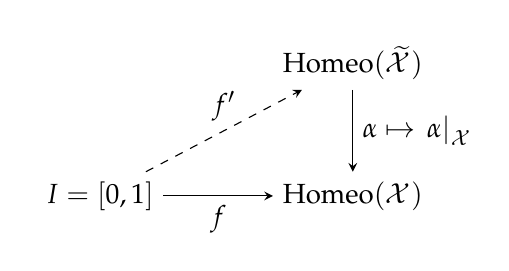
\begin{tikzpicture}
   \matrix (m) [matrix of math nodes,row sep=3em,column sep=4em,minimum width=2em] {
   	& \mathrm{Homeo}(\widetilde{\mathcal{X}}) \\
   	I = [0,1]  & \mathrm{Homeo}(\mathcal{X}) \\};
   \path[-stealth]
   (m-2-1.east|-m-2-2) edge node [below] {$f$}(m-2-2)
   (m-1-2) edge node [right] {$\al \mapsto \left.\a\right|_{\mathcal X}$} (m-2-2)
   (m-2-1)      edge [dashed]  node[above] {$f'$} (m-1-2);
   \end{tikzpicture}
   \hspace{\fill}
   \newline
   where $\mathrm{Homeo}$ means the group of homeomorphisms with {\it compact-open} topology (See \cite{spanier:at}). Above diagram has the following noncommutative generalization   
  \newline
  \hspace*{\fill}
  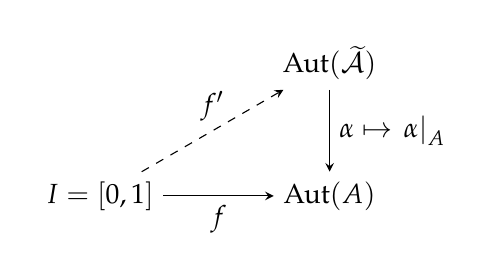
\begin{tikzpicture}
  \matrix (m) [matrix of math nodes,row sep=3em,column sep=4em,minimum width=2em] {
  	& \Aut(\widetilde{\A}) \\
  	I = [0,1]  & \Aut(A) \\};
  \path[-stealth]
  (m-2-1.east|-m-2-2) edge node [below] {$f$}(m-2-2)
  (m-1-2) edge node [right] {$\al \mapsto \left.\a\right|_{A}$} (m-2-2)
  (m-2-1)      edge [dashed]  node[above] {$f'$} (m-1-2);
  \end{tikzpicture}
  \hspace{\fill}
  \newline
   In the above diagram we require that $\al|_A \in \mathrm{Aut}\left(A\right)$ for any $\al \in \mathrm{Aut}\left(\widetilde{A}\right)$. The diagram means that $f'(t)|_{A} = f(t)$ for any $t \in [0,1]$. Noncommutative generalization of a locally compact space is a $C^*$-algebra, so  the generalization of $\mathrm{Homeo}(\mathcal{X})$ is the group  $\mathrm{Aut}(A)$ of *-automorphisms carries (at least) two different topologies making it into a topological group \cite{thomsem:ho_type_uhf}. The most important is {\it the topology of pointwise norm-convergence} based on the open sets
   \begin{equation*}
   	\left\{\left.\alpha \in \mathrm{Aut}(A) \ \right| \ \|\alpha(a)-a\| < 1 \right\}, \ a \in A.
   \end{equation*}
   \paragraph*{} The other topology is the {\it uniform norm-topology} based on the open sets
   \begin{equation}\label{aut_norm_eqn}
   	\left\{\alpha \in \mathrm{Aut}(A) \ \left| \ \sup_{a \neq 0}\ \|a\|^{-1} \|\alpha(a)-a\| < \varepsilon \right. \right\}, \ \varepsilon > 0
   \end{equation}
   which corresponds to following "norm"
   \begin{equation}\label{uniform_norm_topology_formula_eqn}
   	\|\alpha\|_{\text{Aut}} = \sup_{a \neq 0}\ \|a\|^{-1} \|\alpha(a)-a\| = \sup_{\|a\| =1}\  \|\alpha(a)-a\|.
   \end{equation}
   Above formula does not really means a norm because $\mathrm{Aut}\left(A\right)$ is not a vector space. Henceforth the uniform norm-topology will be considered only.

  \begin{definition}\label{upl_f_defn}
	Let $A \hookto \widetilde{A}$  be an inclusion of $C^*$-algebras. Let $f: [0,1] \to  \mathrm{Aut}\left({A}\right)$ be a continuous function such that $f\left( 0\right)= \Id_A$. If  there is a continuous map $\widetilde{f}: [0,1] \to  \mathrm{Aut}\left(\widetilde{A}\right)$ such that $\left.\widetilde{f}(t)\right|_A = f(t)$ for any $t \in \left[0,1\right]$ and $\widetilde{f}\left( 0\right)  = \Id_{\widetilde{A}}$ then we say that $\widetilde{f}$ is a $\pi$-\textit{lift} of $f$. If a lift $\widetilde{f}$ of $f$ is unique then  and map $\widetilde{f}: [0,1] \to  \mathrm{Aut}\left(\widetilde{A}\right)$ is said to be the \textit{unique $\pi$-lift} of $f$. If $\widetilde{f}$ is the unique $\pi$-lift of $f$ then we denote by 
	\be\label{upl_f_eqn}
	\lift_f \stackrel{\text{def}}{=}\widetilde{f}\left(1 \right).
	\ee
\end{definition}
 %  \begin{definition}\label{upl_defn}
%		Let $A \hookto \widetilde{A}$  be an inclusion of $C^*$-algebras.
%	We say that $\pi: A \hookto \widetilde{A}$   has the \textit{unique path lifting} if for any continuous $f: [0,1] \to  \mathrm{Aut}\left({A}\right)$ such that  $f\left( 0\right)= \Id_A$ there is the the unique $\pi$-lift of $f$. The property of unique path lifting will be denoted by $UPL$. The map $\widetilde{f}: [0,1] \to  \mathrm{Aut}\left(\widetilde{A}\right)$ is said to be the \textit{lift} of $f$. 
%\end{definition}
\begin{empt}\label{lift_group_empt}
	Let $\pi: A \hookto \widetilde{A}$  be an inclusion of $C^*$-algebras. Let both $f_1: [0,1] \to  \mathrm{Aut}\left({A}\right)$, $f_2: [0,1] \to  \mathrm{Aut}\left({A}\right)$ have unique $\pi$-lifts $\widetilde{f}_1$ and  $\widetilde{f}_2$ respectively. If $f_1* f_2: [0,1] \to  \mathrm{Aut}\left({A}\right)$, $\widetilde{f}_1* \widetilde{f}_2: [0,1] \to  \mathrm{Aut}\left(\widetilde{{A}}\right)$ are given by
\bean
\left( f_1* f_2\right) \left(t \right) =\left\{
\begin{array}{c l}
f_2\left( 2t\right)  &0 \le t \le \frac{1}{2}  \\
\\
f_1\left(2\left(t - \frac{1}{2} \right)  \right) f_2\left(1\right) & \frac{1}{2} < t \le 1
\end{array}\right.,\\
\left( \widetilde{f}_1* \widetilde{f}_2\right) \left(t \right) =\left\{
\begin{array}{c l}
	\widetilde{f}_2\left( 2t\right)  &0 \le t \le \frac{1}{2}  \\
	\\ \\
	\widetilde{f}_1\left(2\left(t - \frac{1}{2} \right)  \right) \widetilde{f}_2\left(1\right) & \frac{1}{2} < t \le 1
\end{array}\right.
\eean
then $\widetilde{f}_1* \widetilde{f}_2$ is the unique $\pi$-lift of $f_1*f_2$.
Hence one has $\lift_{f_1* f_2}= \lift_{f_1} \lift_{f_2}$.
It turns out that the set of elements $\lift_f$ is a subgroup of $\Aut\left(\widetilde{A}\right)$.
\end{empt}

\begin{defn}\label{lift_group_defn}
		Let $\pi: A \hookto \widetilde{A}$  be an inclusion of $C^*$-algebras then  the group of elements $\lift_f$ (cf. \ref{lift_group_empt}) is said to be the $\pi$-\textit{lift group}.
\end{defn}
\begin{lemma}\label{lift_commutes_lem}
		Let $A \hookto \widetilde{A}$  be an inclusion of $C^*$-algebras. Let $f: [0,1] \to  \mathrm{Aut}\left({A}\right)$ be a continuous function such that $f\left( 0\right)= \Id_A$ and $\widetilde{f}: [0,1] \to  \mathrm{Aut}\left(\widetilde{A}\right)$ is  the \textit{unique $\pi$-lift} of $f$. If $g \in G=\left\{\left. g \in \Aut\left(\widetilde{A} \right)~\right|~ ga = a;~~\forall a \in A\right\}$. Then one has $g\widetilde{f}\left( 1\right) = \widetilde{f}\left( 1\right)g$, i.e. $G$ commutes with the $\pi$-lift group.
\end{lemma}
\begin{proof}
If $\widetilde{f}': [0,1] \to  \mathrm{Aut}\left(\widetilde{A}\right)$ is given by $\widetilde{f}'(t)= g\widetilde{f}(t)g^{-1}$ then $\widetilde{f}'(t)|_A = \widetilde{f}(t)|_A$. From the Definition \ref{upl_f_defn} it turns out $\widetilde{f}'= \widetilde{f}$. It turns out $g\widetilde{f}(1)g^{-1}=\widetilde{f}'(1)=\widetilde{f}(1)$, i.e. one has $\widetilde{f}(1) = g\widetilde{f}(1)g^{-1}$ and, consequently  $\widetilde{f}(1)g = g\widetilde{f}(1)$.
\end{proof}
%\begin{empt}\label{loop_element_empt}
%Let	$\left(A, \widetilde{A}, G, \pi \right)$ be a noncommutaive finite-fold quasi-covering which  has the {unique path lifting}.
%For any $f: [0,1] \to  \mathrm{Aut}\left({A}\right)$ such that $f\left( 0\right)= f\left(1\right)= \Id_A$ and $\widetilde{f}: [0,1] \to  \mathrm{Aut}\left(\widetilde{A}\right)$ such that  that $\widetilde{f}(t)|_A = f(t)$ then $\al = \widetilde{f}\left( 0\right)$ is such that  $\al|_A = \Id_A$, i.e. $\al \in G$. %Moreover if $f': [0,1] \to  \mathrm{Aut}\left({A}\right)$, $f'': [0,1] \to  \mathrm{Aut}\left({A}\right)$ are such that 
%\end{empt}
%\begin{defn}\label{loop_element_defn}
%	Let us consider the situation \ref{loop_element_empt}.
%The element  $\al \in G$ given by \ref{loop_element_empt} is said to be a \textit{loop element}. We say that $\al$ \textit{corresponds} to $f$.
%Clearly a set $L$ of loop elements is a subgroup of $G$, which is said to be the \textit{loop subgroup}. 
%\end{defn}
%\begin{lem}\label{loop_normal_lem}
%	Let	$\left(A, \widetilde{A}, G, \pi \right)$ be a noncommutaive finite-fold quasi-covering which  has the {unique path lifting}. If  $f: [0,1] \to  \mathrm{Aut}\left({A}\right)$ such that $f\left( 0\right)= \Id_A$  and $\widetilde{f}: [0,1] \to  \mathrm{Aut}\left(\widetilde{A}\right)$ such that  that $\widetilde{f}(t)|_A = f(t)$ for any $t \in \left[0,1\right]$ and $\widetilde{f}\left( 0\right)  = \Id_{\widetilde{A}}$ then $g\widetilde{f}(t)g^{-1}= \widetilde{f}(t)$ for any $t \in  [0,1]$.
%\end{lem}
%\begin{proof}
%If $\widetilde{f}': [0,1] \to  \mathrm{Aut}\left(\widetilde{A}\right)$ is given by $\widetilde{f}'(t)= g\widetilde{f}(t)g^{-1}$ then $\widetilde{f}'(t)_A = \widetilde{f}(t)|_A$. From the Definition \ref{upl_defn} it turns out $\widetilde{f}'\cong \widetilde{f}$.
%\end{proof}
%\begin{cor}\label{loop_normal_cor}
%Let	$\left(A, \widetilde{A}, G, \pi \right)$ be a noncommutaive finite-fold quasi-covering which  has the {unique path lifting}. The loop subgroup $L \subset G$ is a normal subgroup of $G$.
%\end{cor}
%\begin{proof}
%Let $g \in G$ and $l \in L$ be any elements, and suppose that $l$ {corresponds} to $f: [0,1] \to  \mathrm{Aut}\left({A}\right)$. If $\widetilde{f}: [0,1] \to  \mathrm{Aut}\left(\widetilde{A}\right)$ is such that $\widetilde{f}(t)|_A = f(t)$ then $ g\widetilde{f}\left( t\right)g^{-1} = \widetilde{f}\left( t\right)$ for all $t \in \left[0,1 \right]$ in particular one has $ g\widetilde{f}\left( 1\right)g^{-1}=\widetilde{f}\left( 1\right)$, or equivalently $glg^{-1}= l$.
%\end{proof}

%\begin{remark}\label{lift_commute_g}
%From the Definition \ref{upl_defn} it turns out that path lift commutes with $G$ i.e. for any lift $\widetilde{f}: [0,1]\to \mathrm{Aut}\left(\widetilde{A}\right)$ and $g \in G$ the map $g\widetilde{f}: [0,1]\to \mathrm{Aut}\left(\widetilde{A}\right)$ is also a lift.
%\end{remark}
\begin{lemma}
		Let $\pi: A \hookto \widetilde{A}$  be an inclusion of $C^*$-algebras.
$f: [0,1] \to  \mathrm{Aut}\left({A}\right)$ be a continuous function such that $f\left( 0\right)= \Id_A$. If  there are two different $\pi$-lifts of $f$ then there is a nontrivial continuous  map: $\widetilde{f}:[0,1] \to  \mathrm{Aut}\left(\widetilde{A}\right)$ such that $\widetilde{f}|_A\left( t\right)  = \id_A$ for every $t \in \left[0,1\right]$.
\end{lemma}
\begin{proof}
	If $\widetilde{f}'$ and $\widetilde{f}''$ are different $\pi$-lifts of $f$ then the map $\widetilde{f}:[0,1] \to  \mathrm{Aut}\left(\widetilde{A}\right)$ given by $t \mapsto \widetilde{f}'\left( t\right)\left(  \widetilde{f}''\left( t\right) \right)^{-1}$ satisfies to conditions of this lemma.
\end{proof}
\begin{cor}\label{lift_unique_cor}
	Let $\pi: A \hookto \widetilde{A}$  be an inclusion of $C^*$-algebras, such that the group 
				\be\nonumber
	G = \left\{ \left.g \in \Aut\left(\widetilde{A} \right)~\right|~ ga = a;~~\forall a \in A\right\}
	\ee
	is finite,  and let   $f: [0,1] \to  \mathrm{Aut}\left({A}\right)$ be such that  $f\left( 0\right)= \Id_A$. If $\widetilde{f}$ is a $\pi$-lift of $f$ then   $\widetilde{f}$ is the unique $\pi$-lift of $f$.
\end{cor}
\begin{proof}
	If there are two different lifts of  $f$  then there is a nontrivial continuous  map: $\widetilde{f}:[0,1] \to  \mathrm{Aut}\left(\widetilde{A}\right)$ such that $\widetilde{f}|_A\left( t\right)  = \id_A$. For any $t \in [0,1]$ one has $\widetilde{f}\left(t \right) \in G$. Since $\widetilde{f}$ is not trivial, the group $G$ is not finite.
\end{proof}

%\begin{lemma}\label{w_path_lift_cor}
%	Let $\pi: A \hookto \widetilde{A}$  be an inclusion of $C^*$-algebras. Suppose $\widetilde{a} \in  \widetilde{A}$ is such that there  is a faithful representation $\rho: \widetilde{A} \to B\left(\H \right)$ such that $\rho\left( \widetilde{a}\right)  \in\rho\left(A \right)''$. If $f: [0,1] \to  \mathrm{Aut}\left({A}\right)$ such that  $f\left( 0\right)= \Id_A$ and both $\widetilde{f}_1, \widetilde{f}_2$ are $\pi$-lifts of $f$ are then $\widetilde{f}_1\left(t\right) \left(\widetilde{a}\right)=\widetilde{f}_2\left(t\right) \left(\widetilde{a}\right)$ for every $t \in [0,1]$. 
%\end{lemma}
%\begin{proof}
%	Since $A$ dense in $\rho\left(A \right)''$ the map $f$ can be uniquely extended up to a continuous map $f'': [0,1] \to  \mathrm{Aut}\left(\rho\left(A \right)''\right)$. From $\rho\left( \widetilde{a}\right)  \in\rho\left(A \right)''$ it turns out $\rho\left(\widetilde{f}_1\left(t\right) \widetilde{a}\right) = \rho\left(\widetilde{f}_2\left(t\right) \widetilde{a}\right)= f''\left( t\right) \left(\rho\left(\widetilde{a} \right) \right)$. Since $\rho$ is faithful one has $\widetilde{f}_1\left(t\right)\left(\widetilde{a}\right)=\widetilde{f}_2\left(t\right) \left(\widetilde{a}\right)$ for each $t \in [0,1]$.
%\end{proof}

%\begin{corollary}\label{borel_path_lift_cor}
%	Let $\pi: A \hookto \widetilde{A}$  be an inclusion of $C^*$-algebras. Suppose $\widetilde{a} \in  \widetilde{A}$ is such that there  is a normal $a \in A$ and Borel measured function $\phi$ such that  $\widetilde{a}= \phi\left( a\right)$. If $f: [0,1] \to  \mathrm{Aut}\left({A}\right)$ such that  $f\left( 0\right)= \Id_A$ and both $\widetilde{f}_1, \widetilde{f}_2$ are $\pi$-lifts of $f$ then $\widetilde{f}_1\left(t\right) \left(\widetilde{a}\right)=\widetilde{f}_2\left(t\right) \left(\widetilde{a}\right)$ for every $t \in [0,1]$.
%\end{corollary}

   \begin{thm}\label{comm_thm}
   	Let $p: \widetilde{\mathcal{X}} \to \mathcal{X}$ be a topological covering projection. Any path $\omega: I \to \mathrm{Homeo}(\mathcal{X})$ such that $\omega(0)=\mathrm{Id}_{\mathcal{X}}$ can be uniquely lifted to the path $\widetilde{\omega}: I \to \mathrm{Homeo}(\widetilde{\mathcal{X}})$ such that $\widetilde{\omega}(0)=\mathrm{Id}_{\widetilde{\mathcal{X}}}$ , i.e. $p(\widetilde{\omega}(t)(x)) = \omega(t)(p(x))$, $\forall t \in [0,1], \ \forall x \in \widetilde{\mathcal{X}}$. It means that the natural *-homomorphism $C_0\left({\mathcal{X}} \right) \hookto C_0\left( \widetilde{\mathcal{X}}\right) $ has the unique path lifting.
   \end{thm}
   \begin{proof}
   	Follows from theorem \ref{spanier_thm_un}.
   \end{proof}

   \section{Coverings of operator spaces}
   \paragraph*{}
   Here we generalize section \ref{cov_fin_bas_sec}.
   \begin{definition}\label{op_su_space_defn}
   	Let $Y$ be an unital operator space, and let $C^*_e\left( Y\right)$ be the $C^*$-envelope (cf. Definition \ref{c_env_sp_defn}) of $Y$. 
   	A \textit{sub-unital} operator space is a pair $\left(X, Y \right)$ where  $X$ is a closed with respect to $C^*$-norm subspace of $Y$ such that $X = Y \oplus \C \cdot 1_{C^*_e\left( Y\right)}$ or $X = Y$.
   \end{definition}

   \begin{remark}
   	Any $C^*$-algebra $A$ naturally yields a {sub-unital} operator space which is $\left(A, A \right)$ is $A$ is unital and $\left(A, A^+ \right)$ otherwise.
   \end{remark}
   \begin{definition}\label{op_sum_space_defn}
   	If both  $\left(X, Y \right)$ and $\left(\widetilde X, \widetilde Y \right)$ are {sub-unital} operator spaces then \textit{complete isometry} from $\left(X, Y \right)$ to $\left(\widetilde X, \widetilde Y \right)$  is a complete unital isometry $\pi_Y: Y \hookto \widetilde Y$ such that $\pi_Y\left(X \right) \subset \widetilde X$. We write
   	\be\label{op_sum_space_eqn}
   	\begin{split}
   	\left( \pi_X: X  \hookto \widetilde X\right) \stackrel{\text{def}}{=} \left.\pi_Y\right|_X;\\
   	\left(\pi_X, \pi_Y \right):  \left(X, Y \right) \hookto \left(\widetilde X, \widetilde Y \right).
   	\end{split}
   	\ee	
   \end{definition}
   \begin{definition}\label{op_su_env_defn}
   	If a pair   $\left(X, Y \right)$ is {sub-unital} operator space then the $C^*$-\textit{envelope} of $\left(X, Y \right)$ is the $C^*$-algebra given by
   \be\label{op_su_env_eqn}
   \begin{split}
   	C^*_e\left( X, Y\right) = \\ = \cap \left\{ \left.A \subset 	C^*_e\left( Y\right)~\right| ~ A  \text{ is a } C^*\text{-subalgebra of } C^*_e\left( Y\right) \text{ AND } X \subset A \right\},
   \end{split}
   \ee
   i.e. $C^*_e\left( X, Y\right)$ is the $C^*$-algebra, generated by $X$.
   \end{definition}
   
   \begin{definition}\label{fin_op_defn}
   Let both $\left(X, Y \right)$ and $\left(\widetilde X, \widetilde Y \right)$ be {sub-unital} operator spaces and let $\left(\pi_X, \pi_Y \right):  \left(X, Y \right) \hookto \left(\widetilde X, \widetilde Y \right)$ be a {complete isometry} from  $\left(X, Y \right)$ to $\left(\widetilde X, \widetilde Y \right)$.
   If  the following conditions hold:
   	\begin{enumerate}
 	\item[(a)] There is a finite-fold  noncommutative covering $\left( C^*_e\left( X,  Y \right), C^*_e\left(\widetilde X, \widetilde Y \right), G, \rho \right)$ (cf. Definition \ref{fin_defn}) such that $\pi_Y = \left.\rho\right|_Y$ and $\pi_X = \left.\rho\right|_X$. 
 	\item[(b)] If $\widetilde X' \subset C^*_e\left(\widetilde X, \widetilde Y \right)$ is a $\C$-linear space  such that $X = \widetilde X' \cap  C^*_e\left( X,  Y \right)$ and $G\widetilde X'= \widetilde X'$  then $\widetilde X' \subseteq \widetilde X$.
 \end{enumerate}
Then we  say that  $\left(\left(X, Y \right),\left(\widetilde X, \widetilde Y \right), G, \left(\pi_X, \pi_Y \right) \right)$   is a  \textit{noncommutative finite-fold covering} of the {sub-unital} operator space $\left(X, Y\right)$.
\end{definition}
\begin{remark}\label{fin_op_g_rem}
The action $G \times C^*_e\left(\widetilde X, \widetilde Y \right) \to C^*_e\left(\widetilde X, \widetilde Y \right)$ is trivial on $C^*_e\left( X,  Y \right)$, so from (b) of the Definition \ref{fin_op_defn} it follows that there is the natural action $G\times \widetilde X \to \widetilde X$ which is trivial on $X$.
\end{remark}



   
   \section{Coverings of spectral triples}\label{triple_fin_cov}

  \paragraph*{}
 
 	Let  $\left( \A, \H, D\right)$ %, \left( \Ga, \right) J\right) $ 
 	be a spectral triple, and let $A$ is the $C^*$-norm completion of $\A$. Let $\left(A, \widetilde{A}, G \right)$ be an unital noncommutative finite-fold covering. Let $\rho: A \to B\left(\H \right)$ be a natural representation given by the spectral triple $\left( \A, \H, D\right)$, and let $\widetilde{\rho}: \widetilde{A} \to B\left( \widetilde{\H}\right)$ be a representation induced by the pair $\left( \rho,\left(A, \widetilde{A}, G \right) \right)$.  
 	The algebra $\widetilde{A}$ is a finitely generated projective $A$-module, it turns out following direct sum
 	$$
 	\widetilde{A} \bigoplus Q \cong A^n.
 	$$
 	of $A$-modules. So there is a projector $p \in \mathbb{M}_n\left(A \right)$ such that
 	$
 		\widetilde{A} \cong pA^n
 	$
 	as $A$-module.  $\A$ is dense in $A$ and $\A$ is closed with respect homomorphic calculus, it turns out that there is a projector $\widetilde{p} \in \mathbb{M}_n\left(\A \right)$ such that $\left\| \widetilde{p} - p\right\|  < 1$, so one has
 	$$
 		\widetilde{A} \cong	\widetilde{p}A^n.
 	$$
 	From $	\widetilde{A} \subset \End_A\left(	\widetilde{A} \right)$ and  $\End_A\left(	\widetilde{A} \right) = \widetilde{p}~\mathbb{M}_n\left(A \right)\widetilde{p} \subset \mathbb{M}_n\left(A \right)$ it follows that there is the following inclusion of $C^*$-algebras
 	$
 	\widetilde{A} \subset \mathbb{M}_n\left(A \right)
 	$. Both $\widetilde{A}$ and $\mathbb{M}_n\left(A \right)$ are finitely generated projective $A$ modules, it turns out that there is an $A$-module $P$ such that
 	$$
 	\widetilde{A} \bigoplus P \cong	\mathbb{M}_n\left(A \right) .
 	$$
 	Taking into account inclusions  $\widetilde{A} \subset \mathbb{M}_n\left(A \right)$ and $\mathbb{M}_n\left(\A \right) \subset \mathbb{M}_n\left(A \right)$ one can define the intersection of algebras
 \begin{equation}\label{a_smooth_eqn}
 	\widetilde{\A}\bydef \widetilde{A} \bigcap \mathbb{M}_n\left(\A \right).
 \end{equation}
 From \cite{varilly_bondia} it turns out that $\mathbb{M}_n\left(\A \right)$ is closed with respect to holomorphic functional calculus.
 	Both $\mathbb{M}_n\left(\A \right)$ and $\widetilde{A}$ are closed with respect to holomorphic functional calculus, so $\widetilde{\A}$ is closed with respect to holomorphic functional calculus, i.e. $\widetilde{\A}$ is a pre-$C^*$-algebra. From 
 	$$
 	\mathbb{M}_n\left(\A \right) \cong \widetilde{\A} \bigoplus \left(P \bigcap 	\mathbb{M}_n\left(\A \right)\right) 
 	$$
 	it turns out that $\widetilde{\A}$ is a finitely generated projective $\A$ module.
 	
 	
  \begin{lemma}\label{dense_lem}
  	The algebra $\widetilde{\A}$ is a dense subalgebra of $\widetilde{A}$ with respect to the $C^*$-norm topology.
  \end{lemma}
\begin{proof}
	There is the isomorphism $A^{n^2}\approx \mathbb{M}_n\left(A \right)$ of right $A$-modules. Since $\widetilde{A}$ is a projective right $A$-module, there is a projector $p_M\in \mathbb{M}_{n^2}\left(A \right)$  it follows that 
	$$
\widetilde{A} \cong p_M A^{n^2}	
	$$
	The algebra $\mathbb{M}_{n^2}\left(\A \right)$ is dense in $\mathbb{M}_{n^2}\left(A \right)$, so there is a projector $\widetilde{p}_M\in \mathbb{M}_{n^2}\left(\A \right)$ such that such that $\left\| \widetilde{p}_M - p_M\right\|  < 1$, it turns out
\be\label{pm_eqn}
	\widetilde{\A} \cong \widetilde{p}_M \A^{n^2}
\ee
For any $\widetilde{a}\in \widetilde{A}$ there is a net $\left\{ \widetilde{a}_\a \in \mathbb{M}_{n}\left(\A \right)\right\}$ such that 
$$
\lim \widetilde{a}_\a = \widetilde{a}
$$
in sense of $C^*$-norm topology. The sequence can be regarded as a sequence $\left\{ \widetilde{a}_\a \in \A^{n^2}\right\}_{n \in \N}$. From \eqref{pm_eqn} it turns out that if $\widetilde{b}_\a=\widetilde{p}_M \widetilde{a}_\a \in \widetilde{A}$ then
$$
\lim \widetilde{b}_\a = \lim \widetilde{p}_M\widetilde{a}_\a = \widetilde{p}_M\lim \widetilde{a}_\a =  \widetilde{p}_M\widetilde{a}=\widetilde{a}.
$$
Otherwise from $\widetilde{a}_\a  \in \A^{n^2}$ and $\widetilde{p}_M\in \mathbb{M}_{n^2}\left(\A \right)$ it turns out that  $\widetilde{b}_\a =\widetilde{p}_M\widetilde{a}_\a  \in \A^{n^2}\cong \mathbb{M}_\a\left(\A \right)$, so one has  $\widetilde{b}_\a  \in \widetilde{A} \bigcap \mathbb{M}_\a\left(\A \right)\cong \widetilde{\A}$. Hence for any $\widetilde{a}\in \widetilde{A}$ there is a sequence $\left\{ \widetilde{b}_\a \in \widetilde{\A}\right\}_{n \in \N}$ such that
$$
\lim \widetilde{b}_\a = \widetilde{a}.
$$
\end{proof}

 \begin{definition}\label{smooth_defn}
 In the above situation we say that the unital noncommutative finite-fold covering $\left(A, \widetilde{A}, G \right)$ is \textit{smoothly invariant} if $G\widetilde{\A} = \widetilde{\A}$.
 \end{definition}
\begin{lem}\label{smooth_matr_lem}
	Let us use the above notation. Suppose that the right $A$-module $\widetilde{A}_A$ is generated by a finite set $\left\{\widetilde{a}_1, \dots, \widetilde{a}_n \right\}$, i.e. 
	$$
	\widetilde{A}_A = \sum_{j =1}^{n} \widetilde{a}_jA,
	$$
	such that following conditions hold:
	\begin{enumerate}
		\item[(a)] $\left\langle \widetilde{a}_j, \widetilde{a}_k\right\rangle_{\widetilde{A}} \in \A$ for any $j,k=1, \dots, n$.
		\item[(b)] The  generated by  $\left\{\widetilde{a}_1, \dots, \widetilde{a}_n \right\}$ right $\A$-module is $G$-invariant, i.e. for all $j = 1,\dots,n$ and $g \in G$ one has
		$g \widetilde{a}_j = \sum_{k=1}^n\widetilde{a}_kc_k$ where $c_k \in \A$ for every $k = 1,\dots,n$.
	\end{enumerate}
Then following conditions hold:
\begin{enumerate}
	\item[(i)] 
	\be\label{smooth_cond_eqn}
	\widetilde{A} \cap \mathbb{M}_n\left(\A \right)= \left\{ 	\widetilde{a}\in 	\widetilde{A}~|~  \left\langle \widetilde{a}_j, \widetilde{a}\widetilde{a}_k\right\rangle_{\widetilde{A}} \in \A; ~\forall j,k =1, \dots, n\right\} 
	\ee
	\item[(ii)] The unital noncommutative finite-fold covering $\left(A, \widetilde{A}, G \right)$ is smoothly invariant (cf. Definition \ref{smooth_defn}).
\end{enumerate}
\end{lem}
\begin{proof}(i)
	If $S \in \End\left( \widetilde{A}\right)_A$ is given by  
\be\label{s_matr}
	S = \sum_{j=1}^{n}\widetilde{a}_j\left\rangle \right\langle\widetilde{a}_j
\ee
	then $S$ is self-adjoint. Moreover $S$ is represented by a matrix $\left\{S_{jk}=\left\langle \widetilde{a}_j, \widetilde{a}_k\right\rangle_{\widetilde{A}} \right\}_{j,k=1,\dots,n} \in \mathbb{M}_n\left( \A\right)$. From the Corollary 1.1.25  of \cite{jensen_thomsen:kk} it turns out that $S$ is strictly positive. Otherwise $\widetilde{A}_A$ is a finitely generated right $A$-module, so from the Exercise  15.O of \cite{wegge_olsen} it follows that $S$ is invertible, i.e. there is $T \in \End\left( \widetilde{A}\right)_A $ such that
	$$
	ST = TS = 1_{\End\left( \widetilde{A}\right)_A}.
	$$
	If we consider $S$ as element of $\mathbb{M}_m\left( \A\right)$ then the spectrum of $S$ is a subset of $\mathcal{U}_0 \bigcup \mathcal{U}_1 \subset \C$ such that
	\begin{itemize}
		\item Both $\mathcal{U}_0$ and $\mathcal{U}_1$ are open sets.
		\item $\mathcal{U}_0 \bigcap \mathcal{U}_1 = \emptyset$,
		\item $0 \in \mathcal{U}_0$ and $0$ is the unique point of the spectrum of $S$ which lies in $\mathcal{U}_0$.
	\end{itemize}
If $\pi, \psi$ are homomorphic functions on $\mathcal{U}_0 \bigcup \mathcal{U}_1$ given by 
\bean\nonumber
\phi|_{\mathcal{U}_0}= \psi|_{\mathcal{U}_0} \equiv 0,\\
\phi|_{\mathcal{U}_1}= 1,\\
\psi|_{\mathcal{U}_1}= z \mapsto \frac{1}{z}~.
\eean
Then following conditions hold:
\begin{itemize}
	\item $p = \phi\left( S\right)$ is a projector, such that $ \widetilde{A}_A \approx p A^n$ as a right $A$-module,
	\item $p \in \mathbb{M}_n\left(\A \right)$,
	\item $\psi\left( S\right) =T\in \mathbb{M}_n\left(\A \right)$ and $TS = ST = 1_{\End\left( \widetilde{A}\right)_A}$. 
\end{itemize}
If $\widetilde{a} \in A$ then from $TS = ST = 1_{\End\left( \widetilde{A}\right)_A}$ it turns out
$$
\widetilde{a} = TS\widetilde{a}ST = T\left( \sum_{j = 1}^n \widetilde{a}_j\left\rangle \right\langle\widetilde{a}_j\right)\widetilde{a}\left( \sum_{k = 1}^n \widetilde{a}_k\left\rangle \right\langle\widetilde{a}_k\right) T= TM^{\widetilde{a}}T
$$
where $M^{\widetilde{a}}\in  \mathbb{M}_n\left(A \right) $ is a matrix given by
$$
M^{\widetilde{a}}=\left\{M^{\widetilde{a}}_{jk}=\left\langle \widetilde{a}_j, \widetilde{a}\widetilde{a}_k\right\rangle_{\widetilde{A}} \right\}_{j,k=1,\dots,n}~.
$$
From $T \in \mathbb{M}_n\left(\A \right)$ it turns out that 
$$
M^{\widetilde{a}} \in \mathbb{M}_n\left(\A \right) \Rightarrow TM^{\widetilde{a}}T\in \mathbb{M}_n\left(\A \right). 
$$
Conversely from $S \in \mathbb{M}_n\left(\A \right)$ it follows that
$$
TM^{\widetilde{a}}T \in \mathbb{M}_n\left(\A \right)\Rightarrow STM^{\widetilde{a}}TS =M^{\widetilde{a}} \in \mathbb{M}_n\left(\A \right), 
$$
so one has
$$
M^{\widetilde{a}} \in \mathbb{M}_n\left(\A \right) \Leftrightarrow TM^{\widetilde{a}}T\in \mathbb{M}_n\left(\A \right). 
$$
Hence
$\widetilde{a} \in \mathbb{M}_n\left(\A \right)$ if and only if $\left\langle\widetilde{a}_j, \widetilde{a}\widetilde{a}_k\right\rangle_{\widetilde{A}}\in \A$ for any $j,k = 1, \dots n$. %From  $TS = ST = 1_{\End\left( \widetilde{A}\right)_A}$ it turns out 
%\be\label{aj_in_sm_eqn}
%\widetilde{a}_j = TS \widetilde{a}_j = T\left( \sum_{k = 1}^n \widetilde{a}_k\left\rangle \right\langle\widetilde{a}_k\right) \widetilde{a}_j = TM^j
%\ee
%where $M^j = \left\{m^j_{kl}\right\}_{k,l=1,\dots,n} \in \mathbb{M}_n\left(\A \right)$ is such that
%$$
%m^j_{kl}=\delta_{kj} \left\langle \widetilde{a}_j, \widetilde{a}_l\right\rangle_{\widetilde{A}} \in \mathbb{M}_n\left(\A \right).
%$$
%From $T \in \mathbb{M}_n\left(\A \right)$ and \eqref{aj_in_sm_eqn} it turns out $\widetilde{a}_j \in \mathbb{M}_n\left(\A \right)$ for any $j =1,\dots n$.
\\
(ii) Note that given by \eqref{finite_hilb_mod_prod_eqn} product is $G$-invariant, i.e. $\left\langle \widetilde{a} , \widetilde{b}  \right\rangle_{\widetilde{A}}= \left\langle g\widetilde{a} , g\widetilde{b}  \right\rangle_{\widetilde{A}}$ for any $g \in G$, it follows that
$$
\left\langle \widetilde{a}_j , \left( g\widetilde{a}\right)  \widetilde{a}_k  \right\rangle_{\widetilde{A}}=\left\langle g^{-1}\widetilde{a}_j , \widetilde{a} \left( g^{-1}\widetilde{a}_k\right)   \right\rangle_{\widetilde{A}}.
$$
Otherwise taking into account the condition (b) of these lemma one has
\bean
g^{-1}\widetilde{a}_j = \sum_{l'=1}^n  \widetilde{a}_{l'}c'_{l'}, \\
g^{-1}\widetilde{a}_k = \sum_{l''=1}^n  \widetilde{a}_{l''}c''_{l''}, \\
\eean
where $c'_{l'}. c''_{l''}\in \A$ for all $l',l'' = 1, \dots n$. It turns out that
$$
\left\langle \widetilde{a}_j , \left( g\widetilde{a}\right)  \widetilde{a}_k  \right\rangle_{\widetilde{A}}=\left\langle g^{-1}\widetilde{a}_j , \widetilde{a} \left( g^{-1}\widetilde{a}_k\right)   \right\rangle_{\widetilde{A}}= \sum_{\substack{l'=1\\l''=1}}^nc'^*_{l'}\left\langle \widetilde{a}_{l'} ,\widetilde{a} \widetilde{a}_{l''}  \right\rangle_{\widetilde{A}}c_{l''} \in \A.
$$

Hence one has $g\left(  \widetilde{A} \bigcap \mathbb{M}_n\left(\A \right)\right) =\widetilde{A} \bigcap \mathbb{M}_n\left(\A \right)
$, or equivalently  $$G\left(  \widetilde{A} \bigcap \mathbb{M}_n\left(\A \right)\right) =\widetilde{A} \bigcap \mathbb{M}_n\left(\A \right)
,$$
hence from \eqref{a_smooth_eqn} one has
$$G\widetilde{\A}  =\widetilde{\A} 
.$$


 


\end{proof}
In the following text we suppose that  the unital noncommutative finite-fold covering $\left(A, \widetilde{A}, G \right)$ is smoothly invariant.
 	 From the Proposition \ref{conn_prop}  it follows that there is a connection
 	$$
 	\nabla' : \widetilde{\A} \to \widetilde{\A} \otimes_{\A} \Om^1_D.
 	$$
Let us define a connection
 	\begin{equation}\label{equiv_eqn}
 	\begin{split}
 	\widetilde{\nabla}:\widetilde{\A} \to \widetilde{\A} \otimes_{\A} \Om^1_D,\\
 	\widetilde{\nabla}\left(\widetilde{a} \right) = \frac{1}{\left|G \right|} \sum_{g \in G} g^{-1}\left(\nabla'\left( g\widetilde{a}\right) . \right)
 	\end{split}
 	\end{equation}
 	The connection $\widetilde{\nabla}$ is $G$-\textit{equivariant}, i.e.
 \be\label{equiv_conn_eqn}
 	\widetilde{\nabla}\left(g\widetilde{a} \right)= g\left( \widetilde{\nabla}\left(\widetilde{a} \right)\right) ; \text{ for any } g \in G, ~\widetilde{a} \in \widetilde{\A}.
 \ee
 
 %	If $\widetilde{a}, 	\widetilde{b} \in 	\widetilde{\A}$ and $\xi \in \H^\infty$ then  from \eqref{d_defn_eqn} it follows that
 %	\be
 %	\begin{split}
 %	\left[\widetilde{D}, \widetilde{a} \right]\left(\widetilde{b} \otimes \xi \right) = \widetilde{D} \left( \left( \widetilde{a} \widetilde{b}\right)\otimes  \xi\right) - a \left( \right) 
 %	\end{split}
% \ee
 \begin{lem}\label{conn_exist_lem} If the unital noncommutative finite-fold covering $\left(A, \widetilde{A}, G \right)$ is smoothly invariant then there is the unique $G$-equivariant connection $$\widetilde{\nabla}:\widetilde{\A} \to \widetilde{\A} \otimes_{\A} \Om^1_D.$$
\end{lem}
\begin{proof} From the equation \eqref{equiv_conn_eqn} it follows that a $G$-equivariant connection exists. Let us prove the uniqueness of it. 
	It follows from the Proposition \ref{conn_prop} that the space of connections is an affine space over the vector space $\Hom_{\sA}\left(\widetilde{\A}, \widetilde{\A} \otimes_{\A} \Om^1_D \right)$.  The space of $G$-equivariant connections is an affine space over the vector space $\Hom^{G}_{\sA}\left(\widetilde{\A}, \widetilde{\A} \otimes_{\A} \Om^1_D \right)$ of $G$-equivariant morphisms, i.e. morphisms in the category $\mathscr{M}^G_{\widetilde{\A}}$ (cf. \ref{fin_gal_cov_sec}). However from  $\ref{fin_gal_cov_sec}$ it follows that the category  $\mathscr{M}^G_{\widetilde{\A}}$ is equivalent to the category $\mathscr{M}_{\A}$ of $\A$-modules. It turns out that there is a 1-1 correspondence between connections
	$$
	\nabla:	\A \to \A \otimes_{\A} \Om^1_D= \Om^1_D
	$$
	and $G$-equivariant connections
	$$
	\widetilde{\nabla}:	\widetilde{\A} \to \widetilde{\A} \otimes_{\A} \Om^1_D.
	$$
	It follows that thee is the unique $G$-equivariant $\widetilde{\nabla}$ connection which corresponds to 
	\begin{equation*}
	\begin{split}
	\nabla:	\A \to \A \otimes_{\A} \Om^1_D= \Om^1_D,\\
	a \mapsto\left[ D, a\right]. 
	\end{split}
	\end{equation*}
	
\end{proof}
\begin{empt}\label{triple_conn_lift_empt}
	Let  $\H^\infty\bydef \bigcap_{n =1}^\infty \Dom D^n$, and let us define an operator $\widetilde{D} : \widetilde{\A} \otimes_{\A} \H^\infty \to \widetilde{\A} \otimes_{\A} \H^\infty$ such that if $\widetilde{a} \in \widetilde{\A}$ and
\begin{equation*}
\begin{split}
\widetilde 	\nabla\left( 	\widetilde{a}\right) = \sum_{j = 1}^m\widetilde{a}_j \otimes \om_j \in \widetilde{\A} \otimes_{\A} \Om^1_D
\end{split}
\end{equation*}
then
\begin{equation}\label{d_defn_eqn}
\widetilde{D}\left(	\widetilde{a} \otimes \xi \right) = \sum_{j = 1}^m\widetilde{a}_j \otimes \om_j\left( \xi\right) + \widetilde{a} \otimes D\xi, \quad \forall\xi \in \H^\infty.
\end{equation}
 	The space $\widetilde{\A} \otimes_{\A} \H^\infty$ is a dense subspace of the Hilbert space $\widetilde{\H} = \widetilde{A} \otimes_{A} \H$,
 	hence  $\widetilde{D}$ can be regarded as an unbounded operator on $\widetilde{\H}$. 
\end{empt}
\begin{defn}\label{triple_conn_lift_defn}
	The operator $\widetilde{D}$ given by \eqref{d_defn_eqn} is said to be the $\left(A, \widetilde{A}, G \right)$-\textit{lift} of $D$. The spectral triple $\left( \widetilde{\A}, \widetilde{\H}, \widetilde{D}\right)$  is said to be the  $\left(A, \widetilde{A}, G \right)$-\textit{lift} of $\left( \A, \H, D \right)$.
\end{defn}
%\begin{rem}
%	From \eqref{equiv_conn_eqn} it follows that the operator $\widetilde{D}$ is equivariant, i.e.
%	\be\label{equiv_d_eqn}
%	\widetilde{D}\left( g \widetilde{\xi}\right) = g \left( \widetilde{D}\widetilde{\xi}\right);~ \forall \widetilde{\xi} \in \Dom \widetilde{G}, ~ \forall g \in G.
%	\ee
%	There are two equivalent ways of definition of operator $\widetilde{D}$ from the Theorem  \ref{st_fin_thm}:
%	\begin{enumerate}
%		\item [(a)] Looking for an operator $\widetilde{ D}$ which satisfies to the Definition \ref{triple_lift_defn},
%		\item[(b)] Application of the equation \eqref{d_defn_eqn}.
%	\end{enumerate}
%\end{rem}
 
 
 
 \section{Finite noncommutative coverings and flat connections}\label{flat_sec}
 \subsection{Basic construction}\label{nc_flat_sec}
 \paragraph*{}
 Let $\left( \A, \H, D\right)$ be a spectral triple, let  $\left( \widetilde{\A}, \widetilde{\H}, \widetilde{D}\right)$ is the $\left(A, \widetilde{A}, G \right)$-lift of $\left( \A, \H, D \right)$. Let $V = \C^n$ and with left action of $G$, i.e. there is a linear representation $\rho: G \to GL\left(\C,n\right)$. Let $\widetilde{\mathcal E} =  \A \otimes \C^{n} \approx \widetilde{\A}^n$ be a free module over $\widetilde{\A}$, so $\widetilde{\mathcal E}$ is a projective finitely generated $\A$-module (because $\widetilde{ \A}$ is a finitely generated projective $\A$-module). Let $\widetilde{\nabla} : \widetilde{\mathcal E} \to \widetilde{\mathcal E} \otimes_{\widetilde{\A}} \Om^1_{\widetilde{D}}$ be the trivial flat connection. In \ref{triple_fin_cov} it is proven that $\Om^1_{\widetilde{D}} = \widetilde{\A}\otimes_{\A}\Om^1_{D}$ it follows that the connection $\widetilde{\nabla} : \widetilde{\mathcal E} \to \widetilde{\mathcal E} \otimes_{\widetilde{\A}} \Om^1_{\widetilde{D}}$ can be regarded as a map $\nabla':\widetilde{\mathcal E} \to \widetilde{\mathcal E} \otimes_{\widetilde{\A}} \widetilde{\A} \otimes_{\A} \Om^1_{\widetilde{D}}= \widetilde{\mathcal E} \otimes_{\A}\Om^1_{{D}}$, i.e. one has a connection
 \be\nonumber
 \nabla':\widetilde{\mathcal E} \to  \widetilde{\mathcal E} \otimes_{\A}\Om^1_{{D}}.
 \ee
 From $\widetilde{\nabla} \circ \widetilde{\nabla} |_{\mathcal E}=0$ it turns out that  $\nabla' \circ \nabla' |_{\mathcal E}=0$, i.e. $\nabla'$ is flat. There is the action of $G$ on $\widetilde{\mathcal E}= \widetilde{\A} \otimes \C^n$ given by 
 \be
 g\left( \widetilde{a}\otimes  x\right)   = g \widetilde{a} \otimes g x; ~~ \forall g \in G,~ \widetilde{a} \in \widetilde{\A}, ~ x \in \C^n.
 \ee
 Denote by
 \be
 \mathcal E = \widetilde{\mathcal E}^G = \left\{\widetilde{\xi} \in  \widetilde{\mathcal E}~|~ G\widetilde{\xi} = \widetilde{\xi}\right\}
 \ee
 Clearly $\mathcal E$ is an $\A$-$\A$-bimodule. For any $\widetilde{\xi} \in \widetilde{\mathcal E}$ there is the unique decomposition
 \be
 \begin{split}
 	\widetilde{\xi} = \xi + \xi_\perp, \\
 	\xi = \frac{1}{\left|G\right|}\sum_{g \in G} g \widetilde{\xi},\\
 	\xi_\perp = \widetilde{\xi} - \xi. 
 \end{split}
 \ee
 From the above decomposition it turns out the direct sum $\widetilde{\mathcal E} = \widetilde{\mathcal E}^G \bigoplus {\mathcal E}_\perp$ of $\A$-modules. So  $\mathcal E = \widetilde{\mathcal E}^G$ is a projective finitely generated $\A$-module, it follows that there is an idempotent $e \in \End_{\A}{\widetilde{\mathcal E}}$ such that $\mathcal E = e \widetilde{\mathcal E}$. The Proposition \ref{conn_prop} gives the canonical connection 
 \be\label{nc_flat_conn}
 \nabla : \mathcal E \to \mathcal E \otimes_{\A} \Om^1_D
 \ee
 which is defined by the connection $\nabla':\widetilde{\mathcal E} \to  \widetilde{\mathcal E} \otimes_{\A}\Om^1_{{D}}$ and the idempotent $e$.
 
 	\begin{lemma}\label{flat_lem}
 	If $\nabla:  \mathcal E \to \mathcal E \otimes_{\A} \Om^1$ is the trivial connection and $e \in \End_{\A}\left( \E\right)$ is an idempotent then the given by \eqref{idem_conn} connection  
 	\bean
 	\nabla_e: e\mathcal E \to e\mathcal E \otimes \Om^1;\\
 	\xi \mapsto \left(e \otimes 1 \right) \nabla \xi	
 \eean
 is flat.
 \end{lemma} 
 \begin{proof}
 	From
 	$$
 	\left(e \otimes 1 \right)\left(\Id_{\mathcal E} \otimes d \right) \circ \left(e \otimes 1 \right)\left(\Id_{\mathcal E} \otimes d \right) = e \otimes d^2 = 0	
 	$$
 	it turns out that $\nabla_e \circ \nabla_e = 0$, i.e. $\nabla_e$ is flat.
 \end{proof}
 \begin{remark}
 	The notion of the trivial connection is an algebraic version of geometrical canonical connection explained in the Section \ref{geom_flat_subsec}.
 \end{remark}
 
 
  From the Lemma \ref{flat_lem} it turns out that the given by \eqref{nc_flat_conn} connection $\nabla$ is flat.
 \begin{definition}
 	We say that  $\nabla$ is a \textit{flat connection induced by} noncommutative covering $\left(A, \widetilde{A}, G\right)$ and the	linear representation $\rho: G \to GL\left(\C,n\right)$, or we say the $\nabla$ \textit{comes from the representation} $\rho: G \to GL\left(\C,n\right)$.
 \end{definition}
 \break

 
 \subsection{Mapping between geometric and algebraic constructions}
 
 \paragraph{}
 The geometric (resp. algebraic) construction of flat connection is explained in the Section \ref{geom_flat_subsec} (resp. \ref{nc_flat_sec}). Following table gives a mapping between these constructions.
 \newline
 
 \begin{tabular}{|c|c|c|}
 	\hline
 	&Geometry & Agebra\\
 	\hline
 	&	&\\
 	1&Riemannian manifold $M$.  & Spectral triple $\left(\Coo\left(M \right), L^2\left(M, \sS \right), \slashed D   \right)$. \\ & & \\
 	2&Topological covering $\widetilde{M} \to M$. & Noncommutative covering, \\ & & $\left(C\left(M \right), C\left(\widetilde{M} \right), G\left( \left.\widetilde{M}~\right|M\right)   \right),$  \\
 	& & given by the Theorem \ref{pavlov_troisky_thm}. \\ & & \\
 	3&Natural structure of Reimannian  & Triple $\left(\Coo\left(\widetilde{M} \right), L^2\left(\widetilde{M}, \widetilde{\sS} \right), \widetilde{\slashed D}   \right)$ is the\\
 	& manifold on the covering space $\widetilde{M}$.&  $\left(C\left(M \right), C\left(\widetilde{M} \right), G\left( \left.\widetilde{M}~\right|M\right)   \right)$ -lift
 	\\
 	&  & of $\left(\Coo\left(M \right), L^2\left(M, \sS \right), \slashed D   \right)$.\\ & & \\
 	4&Group homomorphism   & Action $ G\left( \left.\widetilde{M}~\right|M\right) \times \C^n \to \C^n$\\
 	&$ G\left( \left.\widetilde{M}~\right|M\right) \to GL\left(n, C \right)$ & \\ & & \\
 	5&Trivial bundle $\widetilde{M}\times \C^n$. & Free module $\Coo\left(\widetilde{M} \right) \otimes \C^n$. \\ & & \\
 	6&Canonical flat connection on $\widetilde{M}\times \C^n$ & Trivial flat connection on $\Coo\left(\widetilde{M} \right) \otimes \C^n$\\ & & \\
 	7&Action of $G\left( \left.\widetilde{M}~\right|M\right)$ on $\widetilde{M}\times \C^n$  & Action of $G\left( \left.\widetilde{M}~\right|M\right)$ on  $\Coo\left(\widetilde{M} \right) \otimes \C^n$\\ & & \\
 	8&Quotient space  & Invariant module    \\
 	& $P = \left( \widetilde{M}\times \C^n\right)/G\left( \left.\widetilde{M}~\right|M\right).$& $\mathcal E =  \left( \Coo\left( \widetilde{M}\right) \otimes \C^n\right)^{G\left( \left.\widetilde{M}~\right|M\right)}$ \\ & & \\
 	9&Geometric flat connection on $P$ & Algebraic flat connection on $\mathcal E$.\\ & & \\
 	\hline
 \end{tabular}
 
 \section{Unoriented spectral triples}\label{unoti_defn_sec}
 \paragraph*{}
 Let $M$ be an unoriented  Riemannian manifold, and let $\widetilde{M} \to M$ be a two-fold covering by oriented  Riemannian manifold $\widetilde{M}$ which admits a spin$^c$ structure (cf. Definition \ref{spin_str_defn}). There is an action of $\Z_2 \times \widetilde{M} \to \widetilde{M}$ such that $M \cong \widetilde{M}/ \Z_2$. These 
 considerations inspire the following definition.
 
 \begin{definition}\label{unoriented_defn}
 	Denote by $g \in \Z_2$ the unique nontrivial element.
 	An {\it unoriented spectral triple} $(\A, \H, D)$ consists of:
 	\begin{enumerate}
 		\item
 	A pre-$C^*$-algebra $\A$.
 		\item   An unital noncommutative finite-fold covering $\left(A, \widetilde A, \Z_2\right)$ (cf. Definition \ref{unital_cov_cor}) where $A$ is the $C^*$-norm completion of $\A$.
  		\item A faithful representation $\rho: A \to B\left(\H \right)$. 
 		\item
 		A {selfadjoint operator} $D$ on $\mathcal{H}$, with dense domain
 		$\Dom D \subset \H$, such that $a(\Dom D) \subseteq \Dom D$ for all 
 		$a \in \mathcal{A}$.
 		\item An unital oriented spectral triple $\left(\widetilde{\A}, \widetilde{\H}, \widetilde{D} \right)$ which satisfies to described in  \cite{hajac:toknotes,varilly:noncom} axioms.
 		 	\end{enumerate}
 	Above objects should satisfy to the following conditions:
 		\begin{enumerate}
 			\item[(a)] If $\widetilde{   A}$ is the $C^*$-norm completion of $\widetilde\A$ then the representation $\widetilde A \to \widetilde\H$ is induced by the pair $\left(\rho, \left(A, \widetilde A, \Z_2\right)\right)$ (cf. Definition \ref{fin_uni_defn}).
 			\item[(b)]  The action $\Z_2 \times \widetilde{   A} \to \widetilde{   A}$ of $\Z_2 \cong G\left(\left. \widetilde A~\right|A\right)$ induces the  actions $\Z_2 \times \widetilde{\A} \to  \widetilde{\A} $,  $\Z_2 \times \widetilde{\H} \to  \widetilde{\H} $, such that
 			\be\label{main_def_1_eqn}
 			\begin{split}
 				g \left( \widetilde{a}\widetilde{\xi}\right)= \left(g \widetilde{a}\right) \left(g \widetilde{\xi}\right); ~~ \forall \widetilde{a} \in \widetilde{\A}, ~~ \forall \widetilde{\xi} \in\widetilde{\H},\\
 				\left( g \widetilde{\xi}, g\widetilde{\eta}\right) = \left( \widetilde{\xi}, \widetilde{\eta}\right);~~\forall \widetilde{\xi}, \widetilde{\eta} \in \widetilde{\H},,\\ \text{ where } \left(\cdot, \cdot \right) \text{ is the scalar product on }\widetilde{\H},
 			\end{split}
 			\ee
 			
 			\be\label{main_def_2_eqn}
 			\begin{split}
 				g \left(\widetilde{ D}\widetilde{\xi} \right) = \widetilde{ D}\left(g \widetilde{\xi} \right); ~~  \forall \widetilde{\xi} \in \Dom \widetilde{ D}
 			\end{split}
 			\ee
 	 			\item[(c)] There are natural isomorphisms
 			\be\label{main_def_3_eqn}
 			\begin{split}
 				\A \cong \widetilde{\A}^{\Z_2} \stackrel{\text{def}}{=}\left\{\widetilde{a} \in \widetilde{\A}~|~ g\widetilde{a} = \widetilde{a} \right\},\\
 				\H \cong \widetilde{\H}^{\Z_2}\stackrel{\text{def}}{=} \left\{\widetilde{\xi} \in \widetilde{\H}~|~ g\widetilde{\xi} = \widetilde{\xi} \right\}.
 			\end{split}
 			\ee
 			\item[(d)] If $A$ (resp. $\widetilde{A}$) is a $C^*$-norm completion of $\A$ (resp. $\widetilde{\A}$) then the triple $\left(A, \widetilde{A}, \Z_2 \right)$ is an unital noncommutative finite-fold  covering and the following condition hold:
 			\bea\label{main_def_4_eqn}
 				\A= A\bigcap \widetilde{\A},\\
 	 	\label{main_def_5_eqn}
 				D = \widetilde{ D}|_{\H}=\widetilde{ D}|_{\widetilde{\H}^{\Z_2}}.
  			\eea
 		\end{enumerate}
  \end{definition}
\begin{remark}
The Definition \ref{unoriented_defn} is motivated by explained in the Section \ref{comm_sp_tr} commutative examples. 
\end{remark}

 \chapter{Noncommutative infinite coverings}\label{cov_inf_chap}
 \section{Basic definitions}\label{inf_bas_constr_sec}
\paragraph*{}
This section contains a noncommutative generalization of infinite coverings.
\begin{definition}\label{compliant_covering_defn}
	Let us consider the following diagram\\
	\newline
	\begin{tikzpicture}
	\matrix (m) [matrix of math nodes,row sep=3em,column sep=4em,minimum width=2em]
	{
		\widetilde A_1  &  & \widetilde A_2\\
		& A & \\};
	\path[-stealth]
	(m-1-1) edge[dashed] node [above] {$\pi^1_2$} (m-1-3)
	(m-2-2) edge node [left]  {$\pi_1~~$} (m-1-1)
	(m-2-2) edge node [right] {$~~\pi_2$} (m-1-3);
	%\draw[dashed,->]   (m-1-1) -- (m-1-3);
	\end{tikzpicture}
	\\
	where $A$, $\widetilde A_1$, $\widetilde A_2$ are $C^*$-algebras and $\pi_1$, $\pi_2$, are noncommutative finite-fold coverings. We say that the unordered pair $\left( \pi_1,\pi_2\right) $ is \textit{compliant} if  it satisfies to following conditions:
	\begin{enumerate}
		\item[(a)]
		If there is an injective  *-homomorphism $\pi^1_2: \widetilde A_1 \to \widetilde A_2$ such that $\pi_2 = \pi^1_2 \circ \pi_1$ then $\pi^1_2$ is  a noncommutative finite-fold  covering (cf. Definition \ref{fin_defn}).
		\item[(b)] Following condition holds
		\be\label{g_sur_eqn}
		G\left(\left.\widetilde A_2~\right|A \right)\pi^1_2\left(\widetilde A_1\right)=  \pi^1_2\left(\widetilde A_1\right).
		\ee 
		\item[(c)] From \eqref{g_sur_eqn} it turns out that there is the homomorphism $h: G\left(\left.\widetilde A_2~\right|A \right)\to 	G\left(\left.\widetilde A_1~\right|A \right)$ such that 
		\be\label{g_sur_pi_eqn}
		\pi^1_2\left( h\left(g \right)a_1\right) = g \circ \pi^1_2\left(a_1 \right)
		\ee 
		for each $a_1 \in \widetilde A_1$.  
		We claim that $h$ is surjective. 
		\item[(d)] If  $\rho: \widetilde A_1 \to \widetilde A_2$ is any injective *-homomorphism  such that $\pi_2 = \rho \circ \pi_1$ then there is the unique $g \in 	G\left(\left.\widetilde A_1~\right|A \right)$ such that 
		\be\label{compliant_covering_g_eqn}
		\rho =  \pi^1_2 \circ g.
		\ee
	\end{enumerate}
	
\end{definition}
\begin{definition}\label{compliant_comes_defn}
	In the situation of the Definition \ref{compliant_covering_defn} we say that the homomorphism $h: G\left(\left.\widetilde A_2~\right|A \right)\to 	G\left(\left.\widetilde A_1~\right|A \right)$ which satisfies to \eqref{g_sur_pi_eqn} \textit{comes} from $\pi^1_2$.
\end{definition}
\begin{remark}
	From the Definition \ref{compliant_covering_defn} it turns out that if $\rho': \widetilde A_1 \to \widetilde A_2$ and $\rho': \widetilde A_2 \to \widetilde A_1$ are *-homomorphisms such that $\pi_2 = \rho' \circ \pi_1$ and $\pi_1 = \rho'' \circ \pi_2$ then both $\rho'$ and $\rho''$ are *-isomorphisms.
\end{remark}



\begin{definition}\label{comp_defn}
	Let $\La$ be a countable directed set (cf. Definition \ref{directed_set_defn}) such that there is the unique minimal element $\la_{\min} \in \La$.
	Let $A$ be a $C^*$-algebra.  Let us consider a set noncommutative finite-fold coverings $\mathfrak{S}=\left\{ \pi_{\la}:A \hookto A_{\la}\right\}_{\la \in \La}$ indexed by  $\La$ such that $A_{\la_{\mathrm{min}}}= A$, and $\pi_{\la_{\mathrm{min}}}= \Id_A$. We do not claim that any noncommutative finite-fold covering $A \to \widetilde{A}$ belongs to $\mathfrak{S}$. Suppose that  following conditions hold:
	\begin{enumerate}
		\item[(a)] For any $\mu, \nu \in \La$ a pair $\left( \pi_\mu, \pi_\nu\right)$ is compliant (cf. Definition \ref{compliant_covering_defn}).
		\item [(b)]
		For  $\mu, \nu \in \La$ one has
		\be\label{fg_ord_eqn}
		\begin{split}
			\mu \ge \nu  \text{ if and only if there is an *-homomorphism } \pi: A_\nu \hookto A_\mu; \\
			\text{ such that } \pi_\mu = \pi \circ \pi_\nu.
		\end{split}
		\ee
	\end{enumerate}
	The set 
	$\mathfrak{S}=\left\{ \pi_{\la}:A \hookto A_{\la}\right\}_{\la \in \La}$, or equivalently $$\mathfrak{S}=\left\{ \left( A , A_{\la}, G\left(\left.A_\la~\right|A \right) , \pi_{\la}\right) \right\}_{\la \in \La}$$
	is said to be an \textit{algebraical  finite covering category}. 
	We write $\mathfrak{S} \in \mathfrak{FinAlg}$.
\end{definition}
\begin{remark}\label{implicit_inc_rem}
Below for all $\la\in\La$ we implicitly assume that $A_\la \subset  C^*$-$\varinjlim_{\la \in\La} A_\la$ (cf. Definition \ref{inductive_lim_non_defn}) i.e. for any $\mu, \nu \in \La$ and $a_\mu\in A_\mu, a_\nu\in  A_\nu$ we suppose that both $a_\mu$, $a_\nu$  are elements of the single $C^*$-algebra $C^*$-$\varinjlim_{\la \in\La} A_\la$.
\end{remark}
% \begin{definition}\label{comp_defn}
% 	An algebraical finite precovering category said to be an \textit{algebraical  finite covering category} if all morphism of it are finite-fold coverings.   We write $\mathfrak{S} \in \mathfrak{FinAlg}$
% \end{definition}
\begin{definition}\label{comp_pt_defn}
	A subcategory $\mathfrak{S}^{\text{pt}}$  of an algebraical  finite covering category $\mathfrak{S}$  is said to be a \textit{pointed algebraical  finite covering category}  if it is equivalent to the pre-order category given by $\La$ (cf. Definition \ref{preordercat_defn} and Remark \ref{pre_order_rem}).  We write $\mathfrak{S}^{\text{pt}} \in \mathfrak{FinAlg}^{\text{pt}}$, and use the following notation
	\be\label{comp_pt_eqn}
	\begin{split}
		\mathfrak{S}^{\text{pt}} = \left(\left\{\pi_\la: A \hookto A_\la \right\}_{\la \in \La}, \left\{\pi^\mu_\nu: A_\mu \hookto A_\nu\right\}_{\substack{\mu, \nu \in \La\\ \nu > \mu}}\right),\\
		\text{or simply} \quad \mathfrak{S}^{\text{pt}} = \left(\left\{\pi_\la: A \hookto A_\la \right\}, \left\{\pi^\mu_\nu\right\}\right).
	\end{split}
	\ee
\end{definition}
\begin{remark}\label{comp_pt_rem}
	The Definition \ref{comp_pt_defn} means that for any $\mu \ge \nu$ the category $\mathfrak{S}^{\text{pt}}$ contains the unique *-homomorphism $\pi^\nu_{ \mu}: A_\nu \hookto A_\mu$. The family of $\left\{\pi^\nu_{ \mu}\right\}$ of *-homomorphisms  is said to be a \textit{base-point}.
\end{remark}

\begin{empt}\label{inv_g_lim_empt} Let us consider the situation of the Definition \ref{comp_pt_defn}.
	If $\mu, \nu \in \La$ and $\mu > \nu$. Denote by   $h^\mu_\nu:  G\left(\left.A_\mu~\right|A \right) \to  G\left(\left.A_\nu~\right|A \right)$ the surjective homomorphism which comes from $\pi^\nu_\mu$ (cf. Definition \ref{compliant_comes_defn}).
\end{empt}
\begin{lemma}\label{inv_g_lim_lem}
	Let us use notation of \ref{inv_g_lim_empt}. If $\mu,\la, \nu$ are such that $\mu > \la > \nu$ then $h^\mu_\nu = h^\mu_\la \circ h^\la_\nu$. 
\end{lemma}
\begin{proof}
	From the  equation \eqref{g_sur_pi_eqn} it turns out that for all $a_\nu \in A_\nu$ and $g_\mu \in  G\left(\left.A_\mu~\right|A \right)$ one has
	\bea\label{h_array_eqn}
	\pi^\nu_\mu\left( h^\mu_\nu\left( g_\mu\right)  a_\nu\right)=g_\mu \circ \pi^\nu_\mu\left( a_\nu\right),\\
	\label{h_array1_eqn}
	\pi^\nu_\la\left( h^\la_\nu\left(h^\mu_\la\left(  g_\mu\right) \right)  a_\nu\right)=h^\mu_\la\left(  g_\mu\right) \circ \pi^\nu_\la\left( a_\nu\right),\\
	\label{h_array2_eqn}
	\pi^\la_\mu\left(h^\mu_\la\left( g_\mu\right)\pi^\nu_\la \left(  a_\nu\right) \right)=  g_\mu \circ \pi^\la_\mu\left( \pi^\nu_\la \left(  a_\nu\right)\right)= g_\mu \circ \pi^\nu_\mu \left(  a_\nu\right).
	\eea
	If we substitute $h^\mu_\la\left( g_\mu\right)\pi^\nu_\la \left(  a_\nu\right)$ in the left part of \eqref{h_array2_eqn} by the left part of \eqref{h_array1_eqn} and taking into account $\pi^\la_\mu\circ\pi^\nu_\la=\pi^\nu_\mu$ one has
	\be\label{h_array3_eqn}
	\pi^\la_\mu\left(\pi^\nu_\la\left( h^\la_\nu\left(h^\mu_\la\left(  g_\mu\right) \right)  a_\nu\right) \right)= \pi^\nu_\mu\left( h^\la_\nu\circ h^\mu_\la\left(  g_\mu\right)   a_\nu\right) = g_\mu \circ \pi^\nu_\mu \left(  a_\nu\right).\\
	\ee
	Comparison of \eqref{h_array_eqn} and \eqref{h_array3_eqn} yields $h^\mu_\nu = h^\mu_\la \circ h^\la_\nu$.
\end{proof}


\begin{defn}\label{inv_g_lim_rem}
	From the Lemma \ref{inv_g_lim_lem} it turns out that one can define surjecive homomorphisms  $h^\mu_\nu:  G\left(\left.A_\mu~\right|A \right) \to  G\left(\left.A_\nu~\right|A \right)$ the surjective homomorphism which come from $\pi^\nu_\mu$, hence there is the inverse limit 
	$$
	\widehat{G}=	\varprojlim_{\la \in \La} G\left(\left.A_\la~\right|~A\right)
	$$
	of groups. For any $\la \in \La$ there is the surjecive homomorphism 
	\be\label{h_la_eqn}
	h_\la:\widehat{G}\to G\left(\left.A_\la~\right|~A\right)
	\ee
	Wa say that the  inverse limit \textit{comes} from the base point $\left\{\pi^\nu_\mu\right\}$ (cf Remark \ref{comp_pt_rem}).
\end{defn}

\begin{lemma}\label{base_point_change_lem}
	Let 
	$\mathfrak{S}=\left\{ \left( A , A_{\la},  G\left(\left.A_\la~\right|A \right), \pi_{\la}\right) \right\}_{\la \in \La}\in \mathfrak{FinAlg}$.
	be an {algebraical  finite covering category}.	Consider two pointed subcategories $\mathfrak{S}^{\text{pt}}_\pi$, $\mathfrak{S}^{\text{pt}}_\rho$ having morphisms $\left\{\pi^\nu_\mu: A_{\nu}\hookto A_{
		\mu}\right\}$ and $\left\{\rho^\nu_\mu: A_{\nu}\hookto A_{
		\mu}\right\}$.
	Suppose that both $$\left\{ d^\mu_{\nu} : G\left(\left.A_\mu~\right|A\right) \to G\left(\left.A_\nu~\right|A\right)\right\}  \text{ and }\left\{ e^\mu_{\nu} : G\left(\left.A_\mu~\right|A\right) \to G\left(\left.A_\nu~\right|A\right)\right\} $$ are surjecive homomorphisms which come from $\left\{\pi^\nu_\mu\right\}$ and $\left\{\rho^\nu_\mu\right\}$ respectively. 	Suppose that both $\widehat{G} = \varprojlim_{\la \in \La} G\left(\left.A_\la~\right|A\right)$ and $\widehat{H} = \varprojlim_{\la \in \La} G\left(\left.A_\la~\right|A\right)$ are inverse limits which come from $\left\{ d^\mu_{\nu} \right\} $ and $\left\{ e^\mu_{\nu} \right\} $ respectively. If 
	$d_\la :\widehat{G}\to G\left(\left.A_\nu~\right|A\right)$ and $e_\la :\widehat{H}\to G\left(\left.A_\nu~\right|A\right)$ are natural surjective homomorphisms then there is the bijective map $\phi: \widehat{G} \xrightarrow{\approx} \widehat{H}$ and $\widehat{g}\in \widehat{G}$ such that
	\bea\label{base_point_change_lem_eqn}
	e_\la\circ \phi = d_\la \circ \widehat{g},\\
	\label{base_point_change_p_lem_eqn}
	\rho^\nu_\mu = 	\pi^\nu_\mu \circ d_\nu\left(\widehat{g} \right) \quad \forall \mu > \nu 
	\eea
\end{lemma}
\begin{proof}
	If $\mu \ge \nu$ then there is $g_\nu \in G\left(\left.A_\nu~\right|A\right)$ such that
	\be\label{base_point_change_p_eqn}
	\rho^\nu_\mu =   \pi^\nu_\mu \circ g_\nu.
	\ee From $\pi^\nu_\mu = \pi^\la_\mu \circ \pi^\nu_\la$ and $\rho^\nu_\mu = \rho^\la_\mu \circ \rho^\nu_\la$ one has $d^\mu_\nu\left(g_\mu\right)= g_\nu$. The family $\left\{g_\la\right\}$ gives an element $\widehat{g}\in \widehat{G}$. Any $\widehat{g}' \in \widehat{G}$ corresponds to a family $\left\{g'_\la\right\}_{\la \in \La}$ such that $d^\mu_\nu\left(g'_\mu \right) = g'_\nu$. Otherwise there is the family $\left\{g''_\la\right\}_{\la \in \La}$ such that $g''_\la = g'_\la \circ d_\la \left(  \widehat{g}\right)$ and $e^\mu_\nu\left(g''_\mu \right) = g''_\nu$. The family $\left\{g''_\la\right\}$ uniquely defines the element $\widehat{g}'' \in \widehat{H}$. In result one has the  bijective map
	\bean
	\phi: \widehat{G} \xrightarrow{\approx} \widehat{H},\\
	\widehat{g}' \mapsto \widehat{g}''
	\eean 
	which satisfies to the equation \eqref{base_point_change_lem_eqn}. The equation \eqref{base_point_change_p_lem_eqn} follows from \eqref{base_point_change_p_eqn}.
\end{proof}
\begin{rem}\label{base_point_change_gr_rem}
	The map $\phi$ induces the isomorphism of groups
	\be\label{base_point_change_rem_eqn}
	\begin{split}
		\varphi: \widehat{G} \xrightarrow{\approx} \widehat{H},\\
		\widehat{g}^{~-1}	\widehat{g}'\widehat{g} \mapsto \phi\left( 	\widehat{g}'\right) 
	\end{split}
	\ee
\end{rem}

\begin{rem}\label{base_point_change_rem}
	Let 
	$\mathfrak{S}=\left\{ \left( A , A_{\la},  G\left(\left.A_\la~\right|A\right), \pi_{\la}\right) \right\}_{\la \in \La}\in \mathfrak{FinAlg}$.
	be an {algebraical  finite covering category}. If both 
	$\left\{\pi^\nu_\mu\right\}$ and $ \left\{\rho^\nu_\mu\right\}$ are base-points of $\mathfrak{S}$ then from the Lemma \ref{base_point_change_lem} it turns out the category $\left( \mathfrak{S}, \left\{\pi^\nu_\mu\right\}\right)$ is equivalent to $\left( \mathfrak{S}, \left\{\rho^\nu_\mu\right\}\right)$.
\end{rem}
%\begin{defn}\label{base_point_change_defn}
%	Let $\left(\mathfrak{S}, \left\{\pi^\nu_\mu\right\} \right)\in P$-$\mathfrak{FinAlg}$ to be a  {pointed algebraical  finite covering category}. For any $\widehat{g}\in 	\varprojlim_{\la \in \La} G\left(\left.A_\la~\right|~A\right)$ there is the base point $\left\{\rho^\nu_\mu\right\}$ given by
%	\be\label{base_point_change_eqn}
%	\rho^\nu_\mu = \pi^\nu_\mu\circ h_\nu \left( \widehat{g}\right) 
%	\ee
%	The given by \eqref{base_point_change_defn} replacement of base point  is said to be a \textit{change of base point} (\textit{associated with} $\widehat{g}$).
%\end{defn}
%\begin{remark}
%Any $\widehat{g}\in \widehat{G}$ yields a {change of base point}
%\end{remark}

\begin{remark}
	There is a  functor from $ \mathfrak{S}^{\text{pt}} = \left\{\left\{\pi_\la: A \hookto A_\la \right\}, \left\{\pi^\mu_\nu\right\}\right\}$  to the category of finite groups and epimorphisms. The functor is given by
	\bean
	\left(A \hookto A_\la \right) \mapsto G\left(\left.A_\la~\right|A \right);\\
	\left( \pi^\mu_\nu: A_\nu \hookto A_\mu\right)  \mapsto \left(h^\mu_\nu : G\left(\left.A_\mu~\right|~A\right)\to G\left(\left.A_\nu~\right|~A\right) \right). 
	\eean
\end{remark}





% \begin{remark}\label{cofinal_rem}
% 	If $\La' \subset \La$ is a {cofinal} subset then $\widehat{A} = C^*\text{-}\varinjlim A_{\la}$  be the $C^*$-inductive limit (cf. Definition \ref{inductive_lim_defn}), and suppose that $\widehat{G}= \varprojlim G\left(\left.A_{\la}\right|A \right) $
% 	\be\label{cofinal_eqn}
% 	\begin{split}
% 		C^*\text{-}\varinjlim_{\La} A_{\la} = 	C^*\text{-}\varinjlim_{\La'} A_{\la'},\\
% 		\varprojlim_{\la \in \La}  G\left(\left.A_{\la}\right|A \right)= \varprojlim_{ \La'}  %G\left(\left.A_{\la}\right|A \right).
% 	\end{split}
%	\ee
%	(cf. Proposition \ref{inductive_lim_prop}).
% \end{remark}
\begin{remark}\label{coherent_rem}
	If $\nu \ge \mu$ then since $\mathfrak{S}^{\text{pt}}$ contains the unique injective *-homomorphism $\pi^\mu_{ \nu}: 	A_\mu \hookto A_\nu$, then according to the Remark \ref{implicit_inc_rem} we substitute following equations
	\be\label{coherent_replace_s_eqn}
	\begin{split}
		\pi^\mu_{ \nu}: 	A_\mu \hookto A_\nu,\\
		\pi^\mu_{ \nu}\left( 	a_\mu\right)  = \sum_{g\in G\left(\left.A_\mu~\right|~A_\nu \right)}ga_\nu
	\end{split}
	\ee
	by
	\be\label{coherent_replace_eqn}
	\begin{split}
		A_\mu \subset A_\nu,\\
		a_\mu = \sum_{g\in G\left(\left.A_\mu~\right|~A_\nu \right)}ga_\nu
	\end{split}
	\ee	
	
\end{remark}
Let  $\mathfrak{S}^{\text{pt}} = \left(\left\{\pi_\la: A \hookto A_\la \right\}, \left\{\pi^\mu_\nu\right\}\right)$  be a {pointed algebraical  finite covering category}  (cf. Definition \ref{comp_pt_defn}). Let $\widehat{A} = C^*\text{-}\varinjlim_{\la \in \La} A_{\la}$ be the $C^*$-inductive limit of $C^*$-algebras, and let $\widehat{G}= \varprojlim_{\la \in \La} G\left(
\left.  A_\la~ \right|A\right)$ be the projective limit of groups.
 \begin{definition}\label{equiv_defn}
	A faithful representation ${\pi}: \widehat{A} \hookto B\left( \H\right)$ is said to be \textit{equivariant} if there is the action  $\widehat{G}\times {\H} \to {\H}$ such that
	\be\label{equivt_eqn}
	g \left(\widehat{a}{\xi} \right) = \left(g\widehat{a} \right) \left(g{\xi} \right); \quad \forall g \in \widehat{G},~ \widehat{a} \in \widehat{A},~ {\xi}\in {\H}.
	\ee
\end{definition}
\begin{remark}\label{equiv_rem}
If 	a faithful representation ${\pi}: \widehat{A} \hookto B\left( \H\right)$ is {equivariant} then the action  $\widehat{G}\times {\H} \to {\H}$ induces the natural  action  $\widehat{G}\times B\left( {\H}\right)  \to B\left(  {\H}\right)$ such that
\be\label{equivb_eqn}
\left( ga\right)\xi \bydef  g\left( a \left( g^{-1}\xi\right) \right);\quad \forall g \in \widehat{G},~ a \in B\left(  {\H}\right),~ {\xi}\in {\H}.
\ee


\end{remark}
\begin{lemma}\label{equiv_lem}
	Following conditions hold:
	\begin{enumerate}
		\item [(i)] The universal  representation $\widehat{\pi}: \widehat{A} \hookto B\left( \widehat\H\right)$ (cf. Definition \ref{universal_rep_defn}) is equivariant.
				\item [(ii)] The atomic  representation ${\pi}_a: \widehat{A} \hookto B\left(\widehat \H_a\right)$ (cf. Definition \ref{atomic_repr_defn}) is equivariant.
	\end{enumerate}
\end{lemma}
\begin{proof}
	(i) If $S$ is the state space of $\widehat{A}$ then there is the natural action $\widehat{G}\times S \to S$ given by
	$$
	\left(gs \right) \left(\widehat a\right)\stackrel{\text{def}}{=} s\left(ga \right)
	$$
	where $s \in S$, $g \in \widehat{G}$ and $\widehat{a}\in \widehat{A}$
	Let $s \in S$, and let $L^2\left(\widehat A, s\right)$ is the Hilbert space of the representation $\pi_s:\widehat{A} \to B\left(L^2\left(\widehat A, s\right)\right)$ which corresponds to $s$ (cf. \ref{gns_constr_sec}). If $f_s: \widehat A\to L^2\left(\widehat A, s\right)$ is the given by \ref{from_a_to_l2_eqn} natural $\widehat{A}$-linear map then the $\widehat{A}$-module $f_s\left( \widehat A\right) $ is dense in $L^2\left(\widehat A, s\right)$. Since $$
	\widehat \H = \bigoplus_{s \in S} L^2\left(\widehat A, s\right)
	$$
	the $\C$-linear span of given by
	$$
\xi^s_{\widehat{a}}=\left(0, ..., \underbrace{f_s\left( \widehat{a}\right) }_{s^{\text{th}}-\text{place}}, ..., 0\right)\in \bigoplus_{s \in S} L^2\left(\widehat A, s\right)=		\widehat \H
	$$
elements	is dense in  $\widehat \H$. Hence if for $g \in  \widehat G$ we define
	$$
g \xi^s_{\widehat{a}}\stackrel{\text{def}}{=}	\left(0, ..., \underbrace{f_{gs}\left( g\widehat{a}\right) }_{gs^{\text{th}}-\text{place}}, ..., 0\right)\in \widehat \H
	$$
	then   $g \xi$ can be uniquely defined for all $\xi \in \widehat \H$ i.e. there is the  natural  action $\widehat{G}\times \widehat{\H} \to \widehat{\H}$. Using the equality
	$$
	\widehat a_1 f_s\left(\widehat a_2\right)= f_s\left(\widehat a_1\widehat a_2\right)
	$$
	one can prove that the action $\widehat{G}\times \widehat{\H} \to \widehat{\H}$ satisfies to \eqref{equivt_eqn}.\\
	(ii) The replacement of the "state" word in (i) with "pure state" one gives (ii).
\end{proof}

\begin{definition}\label{special_element_defn}
	Let $\mathfrak{S}^{\mathrm{pt}}=\left(\left\{\pi_\la: A \hookto A_\la \right\}, \left\{\pi^\mu_\nu\right\}\right)\in \mathfrak{FinAlg}^{\mathrm{pt}}$  be a  {pointed algebraical  finite covering category}. $\widehat{A} \bydef C^*\text{-}\varinjlim_{\la \in \La} A_{\la}$ be the $C^*$-inductive limit of $C^*$-algebras, and let $\widehat{G}\bydef \varprojlim_{\la \in \La} G\left(
	\left.  A_\la~ \right|A\right)$ be the projective limit of groups.
	Let $G_\la \bydef \ker\left(  \widehat G\to  G\left(\left.A_\la~\right|~A \right)\right)$, and let $A_{\la}^{\sim}$ be given by \eqref{unital_notation_eqn}. Let $\pi:\widehat{A}\to B\left(\H \right)$ be an equivariant representation. 
	A  positive element $\overline a \in B\left(\H\right)_+$ is said to be $\pi$-\textit{special} if for any $\la_0 \in \La$, $\eps > 0$ and  $z \in A_{\la_0}^{\sim}$
	it satisfies to the following conditions:	
	\begin{enumerate}
		\item[(a)] 	If   $f_\eps: \R \to \R$ is a continuous function given by 
		\begin{equation}\label{f_eps_eqn}
		f_\eps\left( x\right)  =\left\{
		\begin{array}{c l}
		0 &x \le \eps \\
		x - \eps & x > \eps
		\end{array}\right.
		\end{equation}%\label{spec_el_eqn}
		then for all $\la \ge \la_0$  there are $ a_\la, b_\la, a^\eps_\la \in A_\la$ such that
		\be\label{spec_a_eps_eqn}
		\begin{split}
			\sum_{g\in G_\la } \pi \left(z\right)^*\left(  g\overline a\right) \pi\left( z\right)   = \pi\left(a_\la \right),\\
					\sum_{g\in G_\la } f_\eps\left(\pi \left(z\right)^* \left( g\overline a\right) \pi\left( z\right)\right)    = \pi\left(a^\eps_\la \right),\\
			\sum_{g\in G_\la  } \left(\pi \left(z\right)^* \left( g\overline a\right) \pi\left( z\right)\right)^2    = \pi\left(b_\la \right) 
			\end{split}
		\ee
		where sums of the above series mean the strong convergence in  $B\left(\H\right)$ and the action  $G_\la\times B\left(\H\right)\to B\left(\H\right)$ is given by \eqref{equivb_eqn}.
		\item[(b)] There is $\mu \in \La$ such that $\mu \ge \la_0$ and
		\be\label{special_set_eqn}
		\forall \la  \in \La \quad	 \la \ge \mu  \Rightarrow  \left\|a_\la^2 - b_\la\right\| < \eps
		\ee
		where $a_\la, b_\la \in A_\la$ are given by \eqref{spec_a_eps_eqn}.
	\end{enumerate}
	If $\pi$ is the atomic representation then $\overline a$ is said to be \textit{special}.
\end{definition}
\begin{lemma}\label{special_element_cut_lem}
Let $\mathfrak{S}^{\mathrm{pt}}=\left(\left\{\pi_\la: A \hookto A_\la \right\}, \left\{\pi^\mu_\nu\right\}\right)\in \mathfrak{FinAlg}^{\mathrm{pt}}$  be a  {pointed algebraical  finite covering category}. $\widehat{A} \bydef C^*\text{-}\varinjlim_{\la \in \La} A_{\la}$ be the $C^*$-inductive limit of $C^*$-algebras, and let $\widehat{G}\bydef \varprojlim_{\la \in \La} G\left(
\left.  A_\la~ \right|A\right)$ be the projective limit of groups.
Let $G_\la \bydef \ker\left(  \widehat G\to  G\left(\left.A_\la~\right|~A \right)\right)$, and let $A_{\la}^{\sim}$ be given by \eqref{unital_notation_eqn}. Let $\pi:\widehat{A}\to B\left(\H \right)$ be an equivariant representation. 
If  $\overline a \in B\left(\H\right)_+$ is a positive element such that said  for any $\la_0 \in \La$, $\eps > 0$ and  $z \in A_{\la_0}^{\sim}$ there is
$\la'\ge \la_0$ such that $\overline a$ satisfies to \eqref{spec_a_eps_eqn} for all $\la\ge\la'$ then $\overline a$ satisfies to \eqref{spec_a_eps_eqn} for all $\la\ge\la_0$
\end{lemma}
\begin{proof}
The set $\La$ is directed, so for any $\la \ge \la_0$ there is $\la''\in\La$ such that $\la'' \ge\la$ and $\la'' \ge \la'$. There is the surjective homomorphism $G_{\la''}\to G_{\la'}$, such that $G_{\la''}/G_{\la'}\cong G\left(\left. A_{\la''}\right| A_{\la'}\right)$. Let us enumerate $G\left(\left. A_{\la''}\right| A_{\la'}\right)$, i.e.  $G\left(\left. A_{\la''}\right| A_{\la'}\right)=\left\{g_1, ..., g_n\right\}$. If $h: G_{\la'}\to G\left(\left. A_{\la''}\right| A_{\la'}\right)$ is the natural sujective homomorphism then for all $j=1,...,n$ we select $\overline g_j \in G_{\la'}$ such that $h\left(\overline g_j\right)=g_j$. One has
	\be\nonumber
\begin{split}
	\sum_{g\in G_{\la'} } \pi \left(z\right)^*\left(  g\overline a\right) \pi\left( z\right)   =\sum^n_{j=1} \overline g_j \left( 	\sum_{g\in G_{\la''} } \pi \left(z\right)^*\left(  g\overline a\right)\pi\left( z\right)\right)= \sum^n_{j=1} \overline g_j\pi\left(a_{
	\la''} \right)  ,\\
	\sum_{g\in G_{\la'} }f_\eps\left(  \pi \left(z\right)^*\left(  g\overline a\right) \pi\left( z\right)\right)    =\sum^n_{j=1} \overline g_j \left( 	\sum_{g\in G_{\la''} }f_\eps\left(  \pi \left(z\right)^*\left(  g\overline a\right)\pi\left( z\right)\right)\right)= \sum^n_{j=1} \overline g_j\pi\left(a^\eps_{\la''} \right),\\	\sum_{g\in G_{\la'} }\left(  \pi \left(z\right)^*\left(  g\overline a\right) \pi\left( z\right)\right)^2    =\sum^n_{j=1} \overline g_j \left( 	\sum_{g\in G_{\la''} }\left(  \pi \left(z\right)^*\left(  g\overline a\right)\pi\left( z\right)\right)^2 \right)= \sum^n_{j=1} \overline g_j\pi\left(b_{
	\la''} \right) 
\end{split}
\ee
where $a_{	\la''}, b_{\la''}, a^\eps_{\la''}\in A_{\la''}$. From $\overline g_j\pi\left(a_{\la''} \right)= \pi\left(g_ja_{\la''} \right)$, $\overline g_j\pi\left(b_{\la''} \right)= \pi\left(g_jb_{\la''} \right)$ and $\overline g_j\pi\left(a^\eps_{\la''} \right)= \pi\left(g_ja^\eps_{\la''} \right)$ it follows that
	\be\nonumber
\begin{split}
	\sum_{g\in G_{\la'} } \pi \left(z\right)^*\left(  g\overline a\right) \pi\left( z\right)  = \pi\left( \sum_{g'\in G\left(\left. A_{\la''}\right| A_{\la'}\right)} g'a_{\la''} \right)  ,\\
	\sum_{g\in G_{\la'} }f_\eps\left(  \pi \left(z\right)^*\left(  g\overline a\right) \pi\left( z\right)\right)    = \pi\left( \sum_{g'\in G\left(\left. A_{\la''}\right| A_{\la'}\right)} g'a^\eps_{\la''} \right),\\
\	\sum_{g\in G_{\la'} }\left(  \pi \left(z\right)^*\left(  g\overline a\right) \pi\left( z\right)\right)^2    =  \pi\left( \sum_{g'\in G\left(\left. A_{\la''}\right| A_{\la'}\right)} g'b_{\la''} \right).
\end{split}
\ee
However there are $a_{	\la'}, b_{\la'}, a^\eps_{\la'}\in A_{\la'}$ such that
\bean
\pi\left( \sum_{g'\in G\left(\left. A_{\la''}\right| A_{\la'}\right)} g'a_{\la''} \right)= \pi\left(a_{\la'}\right),\\
\pi\left( \sum_{g'\in G\left(\left. A_{\la''}\right| A_{\la'}\right)} g'a^\eps_{\la''} \right)= \pi\left(a^\eps_{\la'}\right),\\
\pi\left( \sum_{g'\in G\left(\left. A_{\la''}\right| A_{\la'}\right)} g'b_{\la''} \right)= \pi\left(b_{\la'}\right).
\eean  
\end{proof}
\begin{lemma}\label{spec_strong_lim_lem}
	Any  $\pi$-special element $\overline a \in B\left( \H\right)_+$ equals to the following strong limit
	\be\label{spec_strong_lim_eqn}
	\overline a = \lim_{\la \in \La}\pi\left(a_\la \right)
	\ee 
	where $a_\la$ satisfies to 	the following equation
	\be\label{spec_a_eqn}
	\begin{split}
		\sum_{g\in G_\la } \pi \left(1_{A^\sim_\la}\right)^*\left(  g\overline a\right) \pi\left(1_{A^\sim_\la}\right)  \cong	\sum_{g\in G_\la } g\overline a   = \pi\left(a_\la \right)
	\end{split}
	\ee	
	(cf. Equation \ref{spec_a_eps_eqn}).
\end{lemma}
\begin{proof}
	The net $\left\{\pi\left(a_\la \right)\right\}_{\la \in \La}$ is decreasing, so from the Theorem \ref{increasing_convergent_w_lem} the strong limit  $\lim_{\a \in \La}\pi\left(a_\la \right)$  exists. The strong limit coincides with the weak one, so one should prove that for all $\xi, \eta \in \H$ one has
	\be\label{spec_strong_limxe_eqn}
	\left(\xi,\overline a \eta \right)= \lim_{\la \in \La} \left(\xi,\pi\left(a_\la \right) \eta \right)= \lim_{\la \in \La}\left(\xi,~~\left( 	\sum_{g\in G_\la }g\overline a \right) \eta \right).
	\ee
	Element $\overline a$ is positive, so from the the polarization equality \eqref{polarization_equality_eqn} it follows that \eqref{spec_strong_limxe_eqn} is equivalent to
	\be\label{spec_strong_limxx_eqn}
	\left(\xi,\overline a \xi \right)=  \lim_{\la \in \La}\left(\xi,~~\left( 	\sum_{g\in G_\la}g\overline a \right) \xi \right)\quad \forall\xi \in \H.
	\ee
	For any $\la \in \La$ one has 
	\be\label{spec_strong_limxx1_eqn}
	\left(\xi,\overline a \xi \right)<\left(\xi,~~\left( 	\sum_{g\in G_\la }g\overline a \right) \xi \right).
	\ee
	Otherwise the nonincreasing net $\left\{x_\la=\left(\xi,~~\left( 	\sum_{g\in \ker\left(  \widehat G\to  G\left(\left.A_\la~\right|~A \right)\right) }g\overline a \right) \xi \right)\right\}$ of real numbers is bounded, so it is convergent. For any $\eps>0$ there is $\la_\eps\in\La$ such that
	$\left|x_\la - \lim_\la x_\la \right| < \eps$ for all $\la \ge \la_\eps$. It follows that 
	\bean
	\la \ge \la_\eps \quad \Rightarrow \\
	\Rightarrow \left|  \left(\xi,~~\left( 	\sum_{\substack{ g\in  G_\la\\g \neq e }}g\overline a \right) \xi \right)-\left(\xi,~~\left( 	\sum_{\substack{ g\in G_\la\\g \neq e }}g\overline a \right) \xi \right)\right|< \eps 
	\eean
	where $e$ is the unity of the group $\widehat G$.
	On the other hand from
	$$
	\bigcap_{\la \in \La}\ker\left(  \widehat G\to  G\left(\left.A_\la~\right|~A \right)\right)= \{e\}
	$$
	it turns out that
	\be\label{spec_strong_limxx2_eqn}
	\forall \la \in \La \quad \la \ge \la_\eps\quad \Rightarrow \quad \left(\xi,\overline a \xi \right)+ \eps >\left(\xi,~~\left( 	\sum_{g\in G_\la }g\overline a \right) \xi \right)
	\ee
	The equation \eqref{spec_strong_limxx_eqn} is a direct consequence of the equations \eqref{spec_strong_limxx1_eqn} and \eqref{spec_strong_limxx2_eqn}.
\end{proof}



\begin{corollary}\label{spec_borel_cor}
	If $\widehat \pi: \widehat A \to B\left(\widehat \H \right)$ is the universal representation then any $\widehat \pi$-special element $\overline a \in B\left(\widehat\H \right)$   lies in the  {enveloping Borel *-algebra} $\mathscr B\left(\widehat A\right)$ of $\widehat A$ (cf. Definition \ref{borel_env_defn}). 
\end{corollary}
\begin{proof}
		Since $\La$ is countable there is an increasing cofinal subset $\left\{\la_n \right\}_{n \in \N} \subset \La$, so one has
	$$
	\lim_{\la \in \La } \widehat \pi\left( a_\la\right)  = \lim_{n \to \infty} \widehat \pi\left( a_{\la_n}\right). 
	$$
	From the above equation and  the Definition \ref{borel_env_defn} it turns out that $\lim_{\la \in \La } \widehat \pi\left( \a_\la\right)  \in \mathscr B\left(\widehat A\right)$. Taking into account \eqref{spec_strong_lim_eqn} one has $\overline a \in \mathscr B\left(\widehat A\right)$.

\end{proof}


\begin{definition}\label{weakly_spec_defn}
	If $\overline a$ is  $\pi$-\textit{special} and $\widehat{x}, \widehat{y} \in \widehat{A}$ then we say that the element
	\be\label{weakly_spec_eqn}
\overline b=	\pi\left(\widehat{x}\right)\overline a \pi\left(\widehat{y}\right)\in B\left(\H\right)
	\ee
is $\pi$-\textit{weakly special}. If $\pi$ is atomic then we say that $\overline b$ is \textit{weakly special}.  Denote by $\Xi_\pi\left( \mathfrak{S}^{\mathrm{pt}}\right)$ the $\widehat{A}$-bimodule of $\pi$-{weakly special} families.
\end{definition}
\begin{empt}\label{disconnected_limit_empt}
	The natural action of $\widehat{G} \times \H \to \H$ induces the action $\widehat{G} \times B\left( \H\right)  \to B\left( \H\right) $. Clearly if $\overline a \in B\left(\H \right)$ is special then $g \overline a$ satisfies to (a), (b) of the Definition \ref{special_element_defn}, i.e. $g \overline a$ is also special. Similarly if $\overline b$ is weakly special then $g \overline b$ is also special, i.e.  there is the natural action
	\be\label{spec_act_eqn}
	\widehat{G}\times \Xi_\pi\left( \mathfrak{S}^{\mathrm{pt}}\right) \to \Xi_\pi\left( \mathfrak{S}^{\mathrm{pt}}\right)
	\ee
There is the natural $\C$-linear map
	\be\label{f_xi_eqn}
	\begin{split}
		f^\Xi_\pi:  \Xi_\pi\left( \mathfrak{S}^{\mathrm{pt}}\right) \to B\left(\H\right)
	\end{split} 
	\ee
	The action \eqref{spec_act_eqn} induces the action
	\be\label{g_a_eqn}
	\widehat{G}\times \overline A_\pi \to \overline A_\pi
	\ee
	where $\overline A_\pi$ is the $C^*$-algebra, generated by $\Xi_\pi\left( \mathfrak{S}^{\mathrm{pt}}\right)$.
\end{empt}

\begin{definition}\label{main_defn_full_defn}
	Let us consider the situation of  \ref{disconnected_limit_empt}. 	The $C^*$-algebra $\overline{A}_\pi\subset B\left(\widehat\H\right)$ generated by the operator space	$f^\Xi_\pi\left( \Xi_\pi\left( \mathfrak{S}^{\mathrm{pt}}\right)\right)$   is said to be the $\pi$-\textit{\it disconnected algebraical inverse noncommutative limit} of $ \mathfrak{S}^{\mathrm{pt}}$. If $G\left(\left.\overline{A}_\pi~\right| A \right)\stackrel{\mathrm{def}}{=} \widehat{G}$ then there is the action of $G\left(\left.\overline{A}_\pi~\right| A\right)\times \overline{A}_\pi\to \overline{A}_\pi$ which comes from the action \eqref{spec_act_eqn}. The triple  $\left(A, \overline{A}_\pi, G\left(\left.\overline{A}_\pi~\right| A \right)\right)$ is said to be the  $\pi$-\textit{disconnected algebraical infinite noncommutative covering} of $ \mathfrak{S}^{\mathrm{pt}} $.  We  say that $G\left(\left.\overline{A}_\pi~\right| A\right)$ is the $\pi$-\textit{disconnected covering transformation group} of $ \mathfrak{S}^{\mathrm{pt}}$.
	If $\pi$ is the atomic representation i.e. $\pi = \pi_a:\widehat{A}\to B\left(\widehat\H_a \right)$ then we write $\overline A$ instead  $\overline{A}_\pi$ and we say that $\overline A$ is the \textit{ disconnected algebraical inverse noncommutative limit} of $ \mathfrak{S}^{\mathrm{pt}}$. Similarly $G\left(\left.\overline{A}~\right| A \right)\stackrel{\mathrm{def}}{=} \widehat{G}$. The triple  $\left(A, \overline{A}, G\left(\left.\overline{A}~\right| A \right)\right)$ is said to be the  \textit{disconnected algebraical infinite noncommutative covering} of $ \mathfrak{S}^{\mathrm{pt}} $.  We  say that $G\left(\left.\overline{A}~\right| A\right)$ is the \textit{disconnected covering transformation group} of $ \mathfrak{S}^{\mathrm{pt}}$.
\end{definition}

\begin{lemma}\label{atomic_universal_lem}
If $\widehat \pi : \widehat{ A}\to B\left( \widehat \H\right)$ is the universal representation then there is the natural *-isomorphism
\be\label{atomic_universal_eqn}
\overline{A}_{\widehat \pi}\cong\overline{A}\bydef\overline{A}_{\widehat \pi_a}.
\ee

\end{lemma}

\begin{proof}
	If $\widehat \pi_a : \widehat{ A}\to B\left( \widehat \H_a\right)$ is the atomic representation then from the Definition \ref{main_defn_full_defn} it follows that $\overline{A} \bydef \overline{A}_{\widehat \pi_a}\subset B\left( \widehat \H_a\right)$.
	From the Theorem \ref{env_alg_thm} it turns out that there is the surjective *-homomorphism $p:\widehat \pi\left( \widehat A\right)''\to \widehat \pi_a\left(\widehat A \right)''$. From the Corollary \ref{atomic_repr_cor} one has the inclusion $\mathscr B\left(\widehat A\right) \subset B\left( \widehat\H_a\right)$ where $\mathscr B\left(\widehat A\right)$ is {enveloping Borel *-algebra}  of $\widehat A$ (cf. Definition \ref{borel_env_defn}). It follows that the restriction 
	$$
	\left.p\right|_{\mathscr B\left(\widehat A\right)}: \mathscr B\left(\widehat A\right) \to p\left(\mathscr B\left(\widehat A\right) \right) 
	$$
	is injective hence $p|_{\mathscr B\left(\widehat A\right)}$ is an *-isomorphism. On the other hand from the Corollary \ref{spec_borel_cor} it turns out that $\overline{A}\subset \mathscr B\left(\widehat A\right)$ so the restriction
	$$
	p|_{\overline{A}_{\widehat \pi}}: \overline{A}_{\widehat \pi} \to p\left( \overline{A}_{\widehat \pi}\right) 
	$$
	is *-isomorphism. If $\overline a_{\widehat \pi} \in \overline{A}_{\widehat \pi}$ is ${\widehat \pi}$-special then 	$\overline a_{\widehat \pi_a}= p|_{\overline{A}_{\widehat \pi}}\left(\overline a_{\widehat \pi}  \right) \in B\left( \widehat\H_a\right)$ is ${\widehat \pi}_a$-special  (cf. Definition \ref{special_element_defn}). It follows that
	$$
 p\left( \overline{A}_{\widehat \pi}\right)\subset  \overline{A}_{\widehat \pi_a}
	$$
	so  there is the natural inclusion
	$$
	 \overline{A}_{\widehat \pi}\subset  \overline{A}_{\widehat \pi_a}
	$$
If $\iota_\H: \widehat\H_a \hookto \widehat\H$ is the natural inclusion and $p_\H: \widehat\H \hookto \widehat\H_a$ is the natural projection then there is the natural inclusion
\bean
\iota: B\left( \widehat\H_a\right)\hookto B\left( \widehat\H\right),\\
a \mapsto \left(\xi \mapsto \iota_\H \left( a p_H\left(\xi \right) \right)  \right) \quad \forall  a \in  B\left( \widehat\H_a\right), ~~ \xi \in   \widehat\H.
\eean	
If $\overline a_{\widehat \pi_a}\in B\left( \widehat\H_a\right)$ is $\widehat \pi_a$-special then direct check shows that  $\overline a_{\widehat \pi}= \iota\left( \overline a_{\widehat \pi_a}\right)\in B\left( \widehat\H\right)$ is  $\widehat \pi$-special. It follows that there is the natural inclusion
	$
\overline{A}_{\widehat \pi_a}\subset  \overline{A}_{\widehat \pi}
$.
Both inclusions $\overline{A}_{\widehat \pi_a}\subset  \overline{A}_{\widehat \pi}$ and $	 \overline{A}_{\widehat \pi}\subset  \overline{A}_{\widehat \pi_a}$ yield the isomorphism $\overline{A}_{\widehat \pi}\cong  \overline{A}_{\widehat \pi_a}$.
\end{proof}

\begin{lemma}\label{inverse_lim_sp_lem}
	If we  consider the situation of \ref{disconnected_limit_empt} and the Definition \ref{main_defn_full_defn} then the  spectrum of $\widehat A$ is the inverse limit of spectra of $A_\la$. 
\end{lemma}

\begin{proof}
	Denote by $\sX_\la$ and $\widehat \sX$ the spectra of $A_\la$ and $\widehat A$ respectively. From the Lemma \ref{cov_spectrum_lem}  it turns out that for any $\mu, \nu \in \La$ such that $\mu > \nu$ the inclusion  $\pi^\nu_{ \mu}: A_\nu \to A_\mu$ induces the surjective continuous map $p^\nu_\mu :  \sX_\mu \to \sX_\nu$. Otherwise if $\sY_\la$ and $\widehat \sY$ are the state spaces of $A_\la$ and $\widehat A$ then one has  $\sX_\la\subset \sY_\la$ and $\widehat \sX\subset \widehat  \sY$. Moreover for any $\mu, \nu \in \La$ such that $\mu > \nu$ there is the natural  continuous surjective map $t^\nu_\mu :  \sY_\mu \to \sY_\nu$ such that
	$$
	p^\nu_\mu = \left.t^\nu_\mu\right|_{\sX_\mu}
	$$
	From the Corollary \ref{inductive_lim_state_nor_cor} it follows that the state space $\widehat \sY = \varprojlim \sY_\la$ of $\widehat A$ is the inverse limit of state spaces of  $A_\la$, i.e. for any $
	\la \in \La$ there is the natural map $\widehat t_\la: \widehat \sY \to \sY_\la$ such that there is the following diagram  
	\newline
	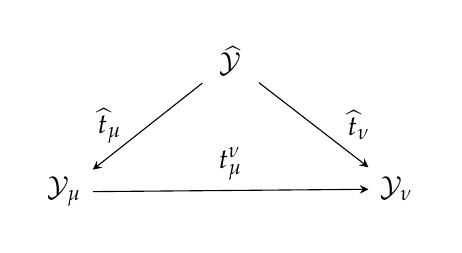
\begin{tikzpicture}
	\matrix (m) [matrix of math nodes,row sep=3em,column sep=4em,minimum width=2em]
	{
		&  \widehat \sY &  \\
		\sY_\mu &  & \sY_\nu \\};
	\path[-stealth]
	(m-1-2) edge node [left] {$\widehat t_\mu~~$} (m-2-1)
	(m-1-2) edge node [right] {$~~~\widehat t_\nu$} (m-2-3)
	(m-2-1) edge node [above] {$t^\nu_\mu$}  (m-2-3);
	
	\end{tikzpicture}
	\newline
	is commutative.	Similarly there is the inverse limit $\widehat \sX = \varprojlim \sX_\la$ and the following  diagram 
	\newline
	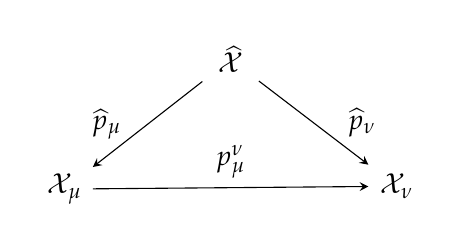
\begin{tikzpicture}
	\matrix (m) [matrix of math nodes,row sep=3em,column sep=4em,minimum width=2em]
	{
		&  \widehat \sX &  \\
		\sX_\mu &  & \sX_\nu \\};
	\path[-stealth]
	(m-1-2) edge node [left] {$\widehat p_\mu~~$} (m-2-1)
	(m-1-2) edge node [right] {$~~~\widehat p_\nu$} (m-2-3)
	(m-2-1) edge node [above] {$p^\nu_\mu$}  (m-2-3);
	\end{tikzpicture}
	\newline
	is commutative. Let $\widehat x \in \widehat \sX$ and let $\widehat \tau : \widehat A \to \C$ be the corresponding functional. Suppose that $ \widehat p: \widehat A \to \C$ is a positive functional such that $\widehat p \le \widehat\tau$. For any $\la\in \La$ following conditions hold:
	\begin{itemize}
		\item The restriction $\left.\widehat p\right|_{A_\la}$ is a positive functional.
		\item There is 	there is a number $t_\la\in \left[0,1\right]$ such that $\left.\widehat p\right|_{A_\la}=t_\la\left.\widehat \tau\right|_{A_\la}$
	\end{itemize}
	If $\mu,\nu\in \La$ are such that $\mu > \nu$ then
	\bean
	\left.\widehat p\right|_{A_\nu}= \frac{1}{\left|G\left( \left.A_\mu \right|A_\nu\right) \right|}\sum_{g \in G\left( \left.A_\mu \right|A_\nu\right)} g \left.\widehat p\right|_{A_\mu},\\
	\left.\widehat \tau\right|_{A_\nu}= \frac{1}{\left|G\left( \left.A_\mu \right|A_\nu\right) \right|}\sum_{g \in G\left( \left.A_\mu \right|A_\nu\right)} g \left.\widehat \tau\right|_{A_\mu}
	\eean
(cf. Lemma \ref{cov_spectrum_lem})	it follows that $t_\mu = t_\nu$, hence there is $t\in \left[0,1\right]$ such that $t_\la=t$ for all $\la\in \La$. So one has $\widehat p= t\widehat\tau$, i.e. $\widehat\tau$ is a pure state.
	Conversely suppose that $\widehat\tau$ is pure and $\left.\widehat \tau\right|_{A_\la}$ is not pure. There is a positive functional  $p_\la: A_\la \to \C$ such that $p_\la \le \left.\widehat \tau\right|_{A_\la}$ and $p_\la \neq t\left.\tau\right|_{A_\la}$ for all $t \in \left[0,1\right]$. Using Hahn�Banach theorem one can extent $p_\la$ up to a positive functional $\widehat p: \widehat A\to \C$ such that $\widehat p\le \widehat \tau$. But $\widehat p \neq t\widehat \tau$ for all $t \in \left[0,1\right]$, i.e. the state $\widehat \tau$ is not pure.
\end{proof}
\begin{lemma}\label{sum_hilb_rep_lem}
	Let $\left\{\H_\la\right\}_{\la\in\La}$ be a family of Hilbert spaces, and let $\H$ be the norm completion of the algebraic direct sum $\oplus_{\la\in\La}\H_\la$. The bounded net $\left\{a_\a\right\}_{\a\in \mathscr A} \in \H$ is strongly convergent  if and only if for all $\la\in\La$ and  $\zeta \in \H$ given by
	$$
	\zeta =\left(0,...~, \underbrace{\zeta_\la}_ {{\la}^{\text{th}}-\mathrm{place}} ,~...,0\right)\in \bigoplus_{\la\in\La}\H_\la
	$$
	 the net $\left\{a_\a\zeta\right\} \in \H$ is norm convergent. 
\end{lemma}
\begin{proof}
If 	$\left\{a_\a\right\}_{\a\in \mathscr A} \in \H$ is strongly convergent then  the net $\left\{a_\a\zeta\right\} \in \H$ is norm convergent for all $\zeta\in \H$.

Conversely suppose that $\left\| a_\a\right\| < C$ for all $\a\in \mathscr A$.
 If	$\xi= \left(\xi_\la\right)_{\la\in \La} \in \H$ 
	and $\eps > 0$ then there is a finite subset   $\La_0\subset \La$ and  $\eta \in \oplus_{\la\in\La}\H_\la$ such that
	\be\label{cunv_un_eqn}
	\eta_{\la}= \begin{cases}
		\xi_{\la}& \la\in \La_0\\
		0& \la\notin \La_0\\
	\end{cases}\text{ AND }	\eta =\left(\eta_{\la}\in \H_{\la}\right)_{\la\in \La}	 \quad \Rightarrow \quad \left\|\xi- \eta\right\|< \frac{\eps} {2C}.
	\ee
	For any $\la \in \La_0$ there is $\a_\la \in \mathscr A$ such that
	\be\label{cunv_2_un_eqn}
	\bt , \ga \ge \a_\la \quad \Rightarrow \quad \left\|\left(a_\bt- a_{\ga}\right)\xi_{\la}\right\|< \frac{\eps} {2\left|\La_0\right|C}
	\ee
	If $\a_{\max} \ge a_\la$ for every $\la\in\La_0$ then  one has 
	\bean
	\bt , \ga \ge \a_{\max} \quad \Rightarrow \quad \left\|\left(a_\bt- a_{\ga}\right)\xi\right\|< \eps.
	\eean
\end{proof}


\begin{empt}
Consider the situation of the Lemma \ref{inverse_lim_sp_lem}. Any $\xi \in \widehat \H_a$ corresponds to the family
\be\label{hat_h_fam_eqn}
\left\{\xi_{\widehat x}\in \H_{\widehat x}\right\}_{\widehat x\in \widehat\sX}.
\ee
\end{empt}
\begin{lemma}\label{spec_el_repr_lem}
Let $\overline a \in B\left( \widehat \H_a\right)_+$ is a special element. There is the family $\left\{\overline a_{\widehat x}\in B\left( \H_{\widehat x}\right) \right\}_{\widehat x\in \widehat\sX}$ such that for any $\widehat\xi \in \widehat \H_a$ given by the family \eqref{hat_h_fam_eqn} element $\overline a\xi$ is represented by the family
$$
\left\{ a_{\widehat x}\xi_{\widehat x}\in \H_{\widehat x}\right\}_{\widehat x\in \widehat\sX}.
$$
\end{lemma}
\begin{proof}
For all $\la \in \La$ we consider the implicit inclusion $A_\la \subset \widehat A$ so for any $\widehat x\in \widehat\sX$ there is the representation $\rep_{\widehat x} :A_\la \to B\left( \sX\right)$. From the Lemma  \ref{spec_strong_lim_lem} it follows that there is the decreasing net $\left\{a_\la\in \widehat A_+\right\}_{\la \in \La}$ such that $a_\la\in A_\la$ and there is the limit $\overline a = \lim_{\la \in \La} a_\la$ with respect to the strong topology of $B\left(\widehat \H_a \right)$. From the Lemma \ref{increasing_convergent_w_lem} for any $\widehat x\in \widehat\sX$ there is the  limit $\overline a_{\widehat x} = \lim_{\la \in \La}\rep_{\widehat x}\left(a_\la\right)$  with respect to the strong topology of $B\left(\widehat \H_{\widehat x} \right)$. If	$\xi \in \widehat\H_a$ is given by the family \eqref{hat_h_fam_eqn}
and $\eps > 0$ then there is a finite subset  is a finite subset $F = \left\{\widehat  x_1,..., \widehat  x_n\right\}\subset \widehat \sX$ such that 
\be\label{rep_1_un_eqn}
\eta_{\widehat x}= \begin{cases}
\xi_{\widehat x}& {\widehat x}\in F\\
0& {\widetilde x}\notin F\\
\end{cases}\text{ AND }	\eta =\left\{\eta_{\widehat x}\in \H_{\widehat x}\right\}_{\widehat x\in \widehat\sX}	 \quad \Rightarrow \quad \left\|\xi- \eta\right\|< \frac{\eps} {2\left\|a\right\|}.
\ee
For any $j = 1, ..., n$ there is $\la_j \in \La$ such that
\be\label{rep_2_un_eqn}
\mu \ge \nu \ge \la_j \quad \Rightarrow \quad \left\|\rep_{\widehat x}\left(a_\mu- a_{\nu}\right)\xi_{\widehat x}\right\|< \frac{\eps} {2n\left\|a\right\|}
\ee
If $\la_{\max} \ge \la_1$ AND  ... AND $\la_{\max} \ge \la_n$ then from the  equations \eqref{rep_1_un_eqn} and \eqref{rep_2_un_eqn} it turns out that if $\zeta$ is represented by the family $\left\{ a_{\widehat x}\xi_{\widehat x}\in \H_{\widehat x}\right\}_{\widehat x\in \widehat\sX}$ then one has 
\bean
\left\|\overline a\xi - \zeta\right\|< \eps.
\eean
\end{proof}
\begin{remark}\label{spec_el_repr_rem}
In the situation of the Lemma \ref{spec_el_repr_lem} denote by
\be\label{spec_el_repr_eqn}
\rep_{\widehat x}\left(\overline a \right) \bydef  \lim_{\la \in \La}\rep_{\widehat x}\left(a_\la\right).
\ee	
\end{remark}

 \begin{definition}\label{main_sdefn}
	Any  maximal connected $C^*$-subalgebra $\widetilde{A}_\pi \subset \overline{A}_\pi$  is said to be a $\pi$-\textit{connected component} of $\mathfrak{S}$. The maximal subgroup $G_\pi\subset G\left(\overline{A}_\pi~|~ A\right)$ among subgroups $G\subset G\left(\overline{A}_\pi~|~ A\right)$ such that $G\widetilde{A}_\pi=\widetilde{A}_\pi$  is said to be the $\widetilde{A}_\pi$-\textit{invariant group} of $\mathfrak{S}^{\mathrm{pt}}$. 
\end{definition}
\begin{definition}\label{mains_defn}
Let	$\mathfrak{S}^{\mathrm{pt}} \in \mathfrak{FinAlg}^{\mathrm{pt}}$, let $\pi: \widehat A \to B\left(\H \right)$ be an equivariant representation.   Suppose that $\left(A, \overline{A}_\pi, G\left(\left.\overline{A}_\pi~\right| A\right)\right)$ is the $\pi$-disconnected infinite noncommutative covering of $\mathfrak{S}$,  $\widetilde{A}_\pi$ is a $\pi$-{connected component} of $\mathfrak{S}^{\mathrm{pt}}$, and $G_\pi$ is the $\widetilde{A}_\pi$-{invariant group} of $\mathfrak{S}^{\mathrm{pt}}$. For any $\la \in \La$ denote by $h_\la: \widehat{G} \to G\left( A_\la~|~A \right)$ the natural surjective homomorphism of groups.
	We say  that $\mathfrak{S}^{\mathrm{pt}}$ is $\pi$-\textit{good} if the following conditions hold:
	\begin{enumerate}
		\item[(a)] For all $\la \in \La$ the natural *-homomorphism $A_\la \to  M\left(\widetilde{A}_\pi \right)$ is injective.
		\item[(b)] If $J\subset G\left(\overline{A}_\pi~|~ A\right)$ is a set of representatives of $G\left(\left.\overline{A}_\pi~\right| A\right)/G_\pi$, then the algebraic direct sum
		\begin{equation*}
		\bigoplus_{g\in J} g\widetilde{A}_\pi
		\end{equation*}
		is a dense subalgebra of $\overline{A}_\pi$.
		\item [(c)] For any $\la \in \La$ the restriction $h_\la|_{G_\pi}$ is an epimorphism, i. e. $h_\la\left(G_\pi \right) = G\left(\left. A_\la~\right|~A \right)$.
	\end{enumerate}
	If $\pi$ is the atomic representation $\pi_a$ then we say $\widetilde A\bydef\widetilde A_\pi$ is a \textit{connected component} of $\mathfrak{S}^{\mathrm{pt}}$ and    $\mathfrak{S}^{\mathrm{pt}}$ is \textit{good}.
\end{definition}
 \begin{definition}\label{main_defn}
	Let $\mathfrak{S}^{\mathrm{pt}} \in \mathfrak{FinAlg}^{\mathrm{pt}}$ be  an algebraical  finite covering category. Let $\pi: \widehat{A} \to B\left(\H \right)$ a representation such that $\mathfrak{S}^{\mathrm{pt}}$ is $\pi$-good.    A connected component $\widetilde{A}_\pi \subset \overline{A}_\pi$  is said to be the $\pi$-\textit{ inverse noncommutative limit of $\mathfrak{S}^{\mathrm{pt}}$}. The $\widetilde{A}_\pi$-invariant group $G_\pi$  is said to be the $\pi$-\textit{covering transformation group of $\mathfrak{S}$}.  The triple $\left(A, \widetilde{A}_\pi, G_\pi\right)$ is said to be the  $\pi$-\textit{infinite noncommutative covering} of $\mathfrak{S}$. %The algebra $A$  is said to be the {\it base algebra} of $\mathfrak{S}$. 
	We will use the following notation 
	\begin{equation*}
	\begin{split}
	\varprojlim_\pi  \mathfrak{S}^{\mathrm{pt}}\stackrel{\mathrm{def}}{=}\widetilde{A}_\pi,\\
	G\left(\left.\widetilde{A}_\pi~\right| A\right)\stackrel{\mathrm{def}}{=}G_\pi.
	\end{split}
	\end{equation*}	
	If $\pi$ is the atomic representation then the subscript $\pi$ will be dropped and we use the words 
\textit{ inverse noncommutative limit of $\mathfrak{S}^{\mathrm{pt}}$},\textit{covering transformation group of $\mathfrak{S}$} and  \textit{infinite noncommutative covering} instead of
	$\pi$-{inverse noncommutative limit of $\mathfrak{S}^{\mathrm{pt}}$}, $\pi$-{covering transformation group of $\mathfrak{S}$} and  $\pi$-{infinite noncommutative covering} respectively.
In this case we write $~\varprojlim  \mathfrak{S}\stackrel{\mathrm{def}}{=}\widetilde{A}$ and  $ G\left(\left.\widetilde{A}~\right| A\right)\stackrel{\mathrm{def}}{=}G$.
\end{definition}
%

\begin{lem}
	Any change of base point yields equivalent weak infinite noncommutative coverings.
\end{lem}
\begin{proof}
	Follows from the Lemma \ref{base_point_change_lem} (cf. Remark \ref{base_point_change_rem})
\end{proof}
%\begin{empt}
%	Although weak infinite noncommutative coverings do not depend on base point modulo isomorphism sometimes it useful to sing explicit dependence on the base point.
%\end{empt}

\begin{remark}\label{main_rem}
	From the condition (b) of the Definition \ref{main_defn} it turns out that  a connected inverse noncommutative limit is unique up to $*$-isomorphism.
\end{remark}

\begin{remark}\label{rep_x_rem}
If $\widehat \sX$ is the spectrum of the $C^*$-inductive limit $C^*$-$\varinjlim_{\la\in\La}A_\la$ then for all $\widehat x$ and $\la\in \La$ there are the natural representations
\be\label{rep_xl_eqn}
\rep_{ \widehat{x}}: A_\la\to B\left(\H_{\widehat{x}}\right).
\ee
From the Lemma \ref{spec_el_repr_lem} it turns out that there are the following natural representations
\be\label{rep_owa_rem}
\begin{split}
\rep_{ \widehat{x}}:\overline A\to B\left(\H_{\widehat{x}}\right),\\
\rep_{ \widehat{x}}: \widetilde A\to B\left(\H_{\widehat{x}}\right)
\end{split}
\ee
(cf. Notation \eqref{spec_el_repr_eqn}).
\end{remark}
\begin{remark}\label{implicit_inc_full_rem}
	Below for all $\la\in\La$ we implicitly assume that $A_\la \subset  B\left(\H \right)$. Similarly the following natural inclusions 
	\bean
	\widehat A \subset B\left(\H \right), \quad
	\overline A_\pi \subset B\left(\H \right), \quad
	\widetilde A_\pi \subset B\left(\H \right), 
	\eean
	will be implicitly used. These inclusions enable us replace the Equations \ref{spec_a_eps_eqn} with the following equivalent system of equations
	\be\label{spec_a_eps_imp_eqn}
	\begin{split}
		\sum_{g\in G_\la } z^*\left(  g\overline a\right) z   \in A_\la,\\
		\sum_{g\in G_\la } f_\eps\left(z^*\left(  g\overline a\right) z   \right)   \in A_\la,\\
		\sum_{g\in G_\la  } \left(z^*\left(  g\overline a\right) z   \right)^2    \in A_\la. 
	\end{split}
	\ee
\end{remark}


\section{Infinite coverings of operator spaces}
\paragraph*{}
Here we consider a generalization of the discussed in the Section \ref{inf_bas_constr_sec} construction.

\begin{empt}\label{comp_op_pt_empt}
	Consider a pointed algebraical  finite covering category (cf. Definition \ref{comp_pt_defn}) given by
	$$
	\mathfrak{S}^{\text{pt}} = \left(\left\{\pi_\la: A \hookto A_\la \right\}_{\la \in \La}, \left\{\pi^\mu_\nu: A_\mu \hookto A_\nu\right\}_{\substack{\mu, \nu \in \La\\ \nu > \mu}}\right),
	$$
	and suppose that $\mathfrak{S}^{\text{pt}}$ is good (cf. Definition \ref{mains_defn}). Assume that for every $\la \in \La$ (including $\la_{\mathrm{min}}$ cf. \ref{comp_defn}) there is a sub-unital operator space $\left(X_\la, Y_\la \right)$ (cf. Definition \ref{op_su_space_defn}) such that $A_\la \cong C^*_e\left(X_\la, Y_\la \right)$ suppose that any $\pi_\la$ and $\pi^\mu_\nu$ corresponds to a noncommutative finite-fold coverings of operator spaces $$\left(\left(X, Y \right) , \left(\left(X_\la, Y_\la \right) \right), G\left(\left.A_\la\right|A \right), \left(\pi^\la_{X_\la}, \pi^\la_{Y_\la}\right)\right)$$ and   
	$$\left(\left(X_\mu, Y_\mu \right) , \left(\left(X_\nu, Y_\nu \right) \right), G\left(\left.A_\mu\right|A_\nu \right), \left(\pi^{\mu\nu}_{X_\mu}, \pi^{\mu\nu}_{Y_\mu}\right)\right)$$
	respectively.
\end{empt}
% \begin{remark}
%	If $A \stackrel{\text{def}}{=} A_{\la_{\mathrm{min}}}$ then	from $B_{\la_{\mathrm{min}}}= B$ it follows that for any $\la \in \La$ the tuple
% 	$$
% 	\left(A, A_\la, B, B_\la, \left.\pi_\la\right|_{A_\la}, \pi_\la, j_{A}, j_{A_\la}, G\left( \left.B_\la \right| B\right)\right)
%	$$
%	is a {noncommutative finite-fold covering of operator algebras}
%\end{remark}
\begin{definition}\label{comp_op_pt_defn}
	Consider the situation \ref{comp_op_pt_empt}. We say that the category 
	\be
	\begin{split}\label{pointed_op_eqn}
		\mathfrak{S}^{\text{pt}}_{\text{op}}
		= \left(\left\{\left( \pi_{X_\la}, \pi_{Y\la}\right) : \left(X, Y \right) \to \left(X_\la, Y_\la \right) \right\}_{\la \in \La},\right. \\
		\left.\left\{\left( \pi^{\nu}_{X_\mu}, \pi^{\nu}_{Y_\mu}\right) : \left(X_\mu, Y_\mu \right) \to \left(X_\nu, Y_\nu \right) \right\}_{\substack{\mu, \nu \in \La\\ \nu > \mu}}\right)
	\end{split}
	\ee
	is a \textit{pointed algebraical  finite covering category of operator spaces}. We write
	\be\label{comp_op_pt_eqn}
	\mathfrak{S}^{\text{pt}}_{\text{op}}\in 	\mathfrak{OSp}^{\text{pt}}_{\text{op}}.
	\ee
\end{definition}
\begin{definition}\label{spec_op_defn}
	Consider the situation of \ref{comp_op_pt_empt} and \ref{comp_op_pt_defn}. 	Let $\widetilde{A}$ be the inverse noncommutative limit of 	$\mathfrak{S}^{\text{pt}}$. Let $\widehat{A}= C^*$-$\varinjlim_{\la \in \La} A_\la$ and $\pi_a:\widehat{A} \to B\left(\H_a \right)$ be the atomic representation. An element $\widetilde x  \in  \widetilde{A}$ is said to be \textit{subordinated} to $\mathfrak{S}^{\text{pt}}_{\text{op}}$ if there is a net $\left\{x_\la \in X_\la\right\}_{\la \in \La}\subset \widehat{A}$ such that
	\be\label{spec_op_eqn}
	\widetilde x = \lim_{\la \in \La } \pi_a\left(x_\la \right)
	\ee
	where the limit of \eqref{spec_op_eqn} implies the strong limit in $B\left(\H_a\right)$.
\end{definition}
\begin{definition}\label{spec_lim_defn}
	Let $\Xi_{\text{op}} \subset \widetilde{A}$ is the space of {subordinated} to $\mathfrak{S}^{\text{pt}}_{\text{op}}$ elements. The $C^*$-norm completion of the $\C$-linear space $\Xi_{\text{op}}$ is said to be the \textit{inverse noncommutative limit} of 	$\mathfrak{S}^{\text{pt}}_{\text{op}}$.
\end{definition}
\begin{remark}
	Since the {inverse noncommutative limit} is a $C^*$-norm closed subspace of $C^*$-algebra $\widetilde A$ it has the natural structure of the operator space.
\end{remark}


\section{Universal  coverings and  fundamental groups}

% \section{Basic construction}
\paragraph{}
Very natural choice of fundamental group is proposed in \cite{milne:etale}, where the fundamental group of algebraic manifold is an inverse limit of finite covering groups. However this theory does not yield the fundamental group, it provides its the profinite completion of the fundamental group. Another way is the construction of the noncommutative universal covering using  construction \ref{inf_bas_constr_sec}. This  construction yields fundamental group in the commutative case $A = C_0\left( \mathcal X\right)$ for described below class of spaces.
\subsection{Universal coverings of $C^*$-algebras}\label{uni_sec}
\begin{definition}\label{fg_bas_defn} 
	Let $A$ be a connected $C^*$-algebra. Let us consider the family $\left\{ \pi_\la:A \hookto A_\la\right\}_{\la \in \La} $ of \textit{all} noncommutative finite-fold coverings of $A$.
Denote by $\mathfrak{S} = \left\{ \pi_\la:A \hookto A_\la\right\}_{\la \in \La}$ and suppose that there is   a  {pointed  algebraical  finite covering category} category $\mathfrak{S}^{\mathrm{pt}} = \left( \left\{ \pi_\la:A \hookto A_\la\right\},\left\{\pi^\nu_\mu\right\} \right)$  which is good.
	The { connected infinite noncommutative covering }  $\left(A, \widetilde{A}, G\left(\left.\widetilde{A}~\right|{A}  \right) \right)$ of $\mathfrak{S}$ is said to be the \textit{universal  covering} of $A$. We also say that $\widetilde{A}$ the \textit{universal  covering} of $A$. The group $G\left(\left.\widetilde{A}~\right|{A}  \right)$  is said to be the \textit{fundamental group} of the pair  $\left( A, \left\{\pi^\nu_\mu\right\}\right) $. We use the following notation
	\be\label{fg_bas_eqn}
	\pi_1\left(A, \left\{\pi^\nu_\mu\right\} \right) \stackrel{\mathrm{def}}{=} G\left(\left.\widetilde{A}~\right|{A} \right).
	\ee

\end{definition}

\begin{remark}\label{fg_bas_rem}
In the Definition \ref{fg_bas_defn} the algebra $\widetilde{A}$ does not depend on a base-point $\left\{\pi^\nu_\mu\right\}$ up to isomorphism (cf. Remark \ref{base_point_change_rem}). 
\end{remark}

%
\begin{lemma}\label{change_point_lem}
Let $\widehat{g} \in \widehat{G}=\varprojlim G\left(\left.A_\la~\right| A,\left\{\pi^\mu_\nu\right\}  \right)$ and let $\rho^\mu_\nu  = \pi^\mu_\nu \circ h_\mu\left( \widehat{g}\right)$ then there is is the natural isomorphism
\be
\begin{split}
		\pi_1\left(A, \left\{\pi^\nu_\mu\right\} \right) \xrightarrow{\approx}	\pi_1\left(A, \left\{\rho^\nu_\mu\right\} \right),\\
		g \mapsto \widehat{g} g \widehat{g}^{-1}.
\end{split}
\ee 
\end{lemma}
\begin{proof}
Follows from the Lemma \ref{base_point_change_lem} (cf. Remark \ref{base_point_change_gr_rem}).
\end{proof}

\subsection{Universal coverings of operator spaces}
\paragraph{} Here the generalization \ref{uni_sec} is being considered here. 
\begin{definition}\label{fg_bas_os_defn} 
	Let $\left(X, Y\right)$ be a {sub-unital} operator space (cf. Definition \ref{op_su_space_defn}). Let us consider the family $\left(\left(X, Y \right) , \left(\left(X_\la, Y_\la \right) \right), G\left(\left.A_\la\right|A \right)\right)$ of \textit{all} noncommutative finite-fold coverings of $\left(X, Y\right)$.
	Denote by $\mathfrak{S} = \left\{ \pi_\la:A \hookto A_\la\right\}_{\la \in \La}$ and suppose that there is   a  {pointed algebraical  finite covering category of operator spaces}  category $\mathfrak{S}^{\mathrm{pt}}_{\text{op}}$  (cf. Definition \ref{comp_op_pt_defn}) given by
		\bean
	\begin{split}
		\mathfrak{S}^{\text{pt}}_{\text{op}}
		= \left(\left\{\left( \pi_{X_\la}, \pi_{Y\la}\right) : \left(X, Y \right) \to \left(X_\la, Y_\la \right) \right\}_{\la \in \La},\right. \\
		\left.\left\{\left( \pi^{\nu}_{X_\mu}, \pi^{\nu}_{Y_\mu}\right) : \left(X_\mu, Y_\mu \right) \to \left(X_\nu, Y_\nu \right) \right\}_{\substack{\mu, \nu \in \La\\ \nu > \mu}}\right)
	\end{split}
	\eean
	The  {inverse noncommutative limit} of $\mathfrak{S}^{\text{pt}}_{\text{op}}$ \ref{spec_lim_defn} is said to be  the \textit{universal  covering} of $\left(X, Y \right)$. If 	$C^*_e\left( X, Y\right)$ is the $C^*$-\textit{envelope} of $\left(X, Y \right)$ then the fundamental group  $\pi_1\left( C^*_e\left( X, Y\right), \left\{\pi^\nu_\mu\right\} \right) $ is said to be the \textit{fundamental group} of $\left(X, Y \right)$. We write
		\be\label{fg_bas_os_eqn}
	\pi_1\left(\left(X, Y \right) , \left\{\pi^\nu_\mu\right\} \right)\bydef	\pi_1\left(C^*_e\left(X, Y \right) , \left\{\pi^\nu_\mu\right\} \right)
	\ee
	
\end{definition}
 

\begin{remark}\label{fg_bas_os_rem}
If $\widetilde X$ is the universal covering of $\left(X, Y\right)$ and $\widetilde{C^*_e\left(X, Y \right)}$ is the universal covering of $C^*_e\left(X, Y \right)$ then there is the natural inclusion $\widetilde X \subset \widetilde{C^*_e\left(X, Y \right)}$. Otherwise if $\pi_1\left(C^*_e\left(X, Y \right) , \left\{\pi^\nu_\mu\right\} \right) \times C^*_e\left(X, Y \right)\to C^*_e\left(X, Y \right)$ is the natural action then $\pi_1\left(C^*_e\left(X, Y \right) , \left\{\pi^\nu_\mu\right\} \right) \widetilde X = \widetilde X$, hence from  \eqref{fg_bas_os_eqn} it follows the existence of the natural action
 \be\label{fg_bas_act_os_eqn}
 \pi_1\left(\left(X, Y \right) , \left\{\pi^\nu_\mu\right\} \right)\times 	\widetilde X \to \widetilde X.
 \ee
\end{remark}
\begin{remark}
	The both  notions of the universal covering and the fundamental group of a $C^*$-algebra are specializations of the universal covering and the fundamental group of an operator space.
\end{remark}

%


 \section{Induced representations}\label{inf_ind_repr_subsection}

   \begin{definition}\label{inf_hilb_prod_defn}
 	Let $\mathfrak{S}^{\text{pt}} = \left(\left\{\pi_\la: A \hookto A_\la \right\}, \left\{\pi^\mu_\nu\right\}\right)\in \mathfrak{FinAlg}^{\text{pt}} $ be  a pointed algebraical  finite covering  category.  Let $\pi: C^*$-$\varinjlim_{\la \in \La} A_\la \to B\left(\widehat \H\right)$ be an equivariant representation such that $\mathfrak{S}^{\text{pt}}$ is $\pi$-good (cf. Definition \ref{mains_defn}).  Let  $$\left(A, \widetilde{A}_\pi, G\left(\left.\widetilde{A}_\pi~\right|A \right) \right)$$  be an  infinite noncommutative covering of $\mathfrak{S}^{\text{pt}}$. Let $K\left( \widetilde{A}_\pi\right)$ be the Pedersen's ideal of  $\widetilde{A}_\pi$ (cf. Definition \ref{peder_id_defn}). We say that $\widetilde{A}_\pi$ \textit{allows the inner product} if for any $\la \in \La$, and $\widetilde{a}, \widetilde{b} \in K\left( \widetilde{A}_\pi\right)$ the series
 		\begin{equation*}
 		\begin{split}
 		a_{\la} = \sum_{g \in \ker\left(G\left(\left.\widetilde{A}_\pi~\right|A \right)  \to  G\left( A_{\la}~|~A \right)\right)} g \left(\widetilde{a}^* \widetilde{b}  \right) 
 		\end{split}
 		\end{equation*}
 		is  convergent with respect to the strict topology (cf. Definition \ref{strict_topology})of $M\left( \widetilde{A}_\pi\right)$ and $a_{\la} \in A_{\la}$.
 	Also we say that $\left( A, \widetilde{A}_\pi, G\left(\left.\widetilde{A}_\pi~\right|A \right) \right)$ \textit{allows the inner product}.
 \end{definition}
\begin{rem}\label{inf_hilb_prod_low_rem}
	Let $\mathfrak{S}^{\text{pt}} = \left(\left\{\pi_\la: A \hookto A_\la \right\}, \left\{\pi^\mu_\nu\right\}\right)\in \mathfrak{FinAlg}^{\text{pt}} $ be  a pointed algebraical  finite covering category.   Let $\left(A, \widetilde{A}_\pi, G\left(\left.\widetilde{A}_\pi~\right|A \right) \right)$  be a weak  infinite noncommutative covering of $\mathfrak{S}$. Let $K\left( \widetilde{A}_\pi\right)$ be the Pedersen's ideal of  $\widetilde{A}_\pi$. If there  is $\la_0 \in \La$ such that for any $\widetilde{a}, \widetilde{b} \in K\left( \widetilde{A}_\pi\right)$ such that
	\begin{equation}\nonumber
	\begin{split}
	c_{\la_0} = \sum_{g \in \ker\left(G\left(\left.\widetilde{A}_\pi~\right|A \right)  \to  G\left( A_{\la_0}~|~A \right)\right)} g \left(\widetilde{a}^* \widetilde{b}  \right) \in A_{\la_0}
	\end{split}
	\end{equation}
	then for any $\la < \la_0$ one has
	\begin{equation}\nonumber
	\begin{split}
	c_{\la} = \sum_{g \in \ker\left(G\left(\left.\widetilde{A}_\pi~\right|A \right)  \to  G\left( A_{\la}~|~A \right)\right)} g \left(\widetilde{a}^* \widetilde{b}  \right) =
	\sum_{g \in  G\left( A_{\la_0}~|~A_\la \right)} g c_{\la_0}
	\in A_{\la}.
	\end{split}
	\end{equation}
\end{rem} 
\
 
 \begin{rem}\label{inf_hilb_prod_rem}
 	If $\mathfrak{S}^{\text{pt}}$ allows  inner product  then $K\left( \widetilde{A}_\pi\right)$ is a pre-Hilbert $A$ module such that the inner product is given by
 	\begin{equation*}
 	\begin{split}
 	\left\langle \widetilde{a}, \widetilde{b}  \right\rangle_A  = \sum_{g \in  G\left(\left.\widetilde{A}_\pi~\right|A \right)} g \left(\widetilde{a}^* \widetilde{b}  \right) \in A 
 	\end{split}
 	\end{equation*}
 	where the above series is convergent with respect to the strict topology of $M\left( \widetilde{A}_\pi\right)$. The completion of  $K\left( \widetilde{A}_\pi\right)$ with respect to a norm
 	\begin{equation}\label{inf_hilb_norm_eqn}
 	\begin{split}
 	\left\| \widetilde{a}\right\| = \sqrt{\left\| \left\langle \widetilde{a}, \widetilde{a}  \right\rangle_A\right\|}
 	\end{split}
 	\end{equation}
 	is a Hilbert  $A$-premodule. Denote by $X_A$ this completion. The ideal $K\left( \widetilde{A}_\pi\right)$ is a left $\widetilde{A}_\pi$-module, so $X_A$ is also $\widetilde{A}_\pi$-module. Sometimes we will write  $_{\widetilde{A}_\pi}X_A$ instead  $X_A$.
Moreover since  $K\left( \widetilde{A}_\pi\right)$ is $A$-bimodule and $\widetilde{A}_\pi$-bimodule  $_{\widetilde{A}_\pi}X_A$ is also $A$-bimodule and $\widetilde{A}_\pi$-bimodule. Since the given by \eqref{inf_hilb_norm_eqn} norm exceeds the $C^*$-norm of  $\widetilde{A}_\pi$ there is the natural inclusion 
\be\label{inf_hilb_inc_eqn}
_{\widetilde{A}_\pi}X_A\subset \widetilde{A}_\pi
\ee
 \end{rem}
\begin{definition}\label{inf_hilb_mod_defn}
 	Let $\mathfrak{S}^{\text{pt}} = \left(\left\{\pi_\la: A \hookto A_\la \right\}, \left\{\pi^\mu_\nu\right\}\right) \in \mathfrak{FinAlg}^{\text{pt}}$ and  $\mathfrak{S}^{\text{pt}}$ allows inner product (with respect to $\pi$) then $K\left( \widetilde{A}_\pi\right)$ then we say that given by the Remark  \ref{inf_hilb_prod_rem} $A$-Hilbert module $_{\widetilde{A}_\pi}X_A$ \textit{corresponds to } $\widetilde{A}_\pi$.
 \end{definition}
 
 

 
 \begin{defn}\label{induced_repr_inf_defn}
 	Let $\mathfrak{S}^{\text{pt}} = \left(\left\{\pi_\la: A \hookto A_\la \right\}, \left\{\pi^\mu_\nu\right\}\right)\in \mathfrak{FinAlg}^{\text{pt}}$ and  let $$\left(A, \widetilde{A}_\pi, G\left(\left.\widetilde{A}_\pi~\right|A \right) \right)$$  be a weak  infinite noncommutative covering of $\mathfrak{S}^{\text{pt}}$. Suppose $\widetilde{A}_\pi$ allows inner product   and $A$-Hilbert module $_{\widetilde{A}_\pi}X_A$ corresponds to $\widetilde{A}_\pi$.  Suppose  $\rho: A \to B\left( \H\right)$ is a representation and   $\widetilde{\rho}=_{\widetilde{A}_\pi}X_A-\Ind^A_{\widetilde{A}_\pi}\rho: \widetilde{A}_\pi\to B\left(\widetilde{\H} \right) $ is given by \eqref{ind_repr_eqn}, i.e. $\widetilde{\rho}$ is the induced representation (cf. Definition \ref{ind_repr_defn}) 
 The representation  $\widetilde{\rho}:\widetilde{A}_\pi \to  B\left( \widetilde{\H}\right)$ is said to be \textit{induced} by  $\rho$. We also say that  $\widetilde{\rho}$ is  \textit{induced} by $\left( \rho, \left( A, \widetilde{A}_\pi, G\left(\left.\widetilde{A}_\pi~\right|A \right) \right)\right) $. 
 \end{defn}
 \begin{rem}
 	If $\rho$ is faithful, then  $\widetilde{\rho}$ is faithful.
 \end{rem}
\begin{rem}\label{a_act_hilb_rem} 
 	There is the action of $G\left(\left.\widetilde{A}_\pi~\right|A \right)$ on $\widetilde{\H}$ which comes from the natural action of $G\left(\left.\widetilde{A}_\pi~\right|A \right)$ on the $\widetilde{A}_\pi$-bimodule $K\left( \widetilde{A}_\pi\right) $. If the representation $\widetilde A \to 	B\left( \widetilde{\H} \right)$ is faithful then an action of  $G\left(\left.\widetilde{A}_\pi~\right|A \right)$ on $\widetilde{A}_\pi$ is given by
 	\be\label{ind_h_ind_a_eqn}
 	\left( g  \widetilde a\right) \xi =   g \left(  \widetilde a  \left(  g^{-1}\widetilde\xi\right) \right); ~ \forall  g  \in {G}, ~ \forall\widetilde a  \in \widetilde{A}_\pi, ~\forall\widetilde \xi \in \widetilde{\H}.
 	\ee
 \end{rem}
\begin{rem}\label{ap_act_hilb_rem} 
 If  $\widetilde{\rho}:\widetilde{A}_\pi \to  B\left( \widetilde{\H}\right)$ is   {induced} by $\left( \rho, \left( A, \widetilde{A}_\pi, G\left(\left.\widetilde{A}_\pi~\right|A \right) \right)\right) $ then $\widetilde{\H}$ is the completion of the pre-Hilbert space $K\left( {\widetilde{A}_\pi}\right) \otimes_A \H$ with given by
 \be\label{comp_hilb_eqn}
 \left(\widetilde{a} \otimes \xi, \widetilde{b} \otimes \eta \right)_{\widetilde{\H}} = \left( \xi, \left\langle \widetilde{a} , \widetilde{b} \right\rangle_A \eta\right)_{\H} \quad \forall \widetilde{a} \otimes \xi,~ \widetilde{b} \otimes \eta \in K\left(\widetilde{A}_\pi\right) \otimes \H
 \ee
 scalar product. The action $\widetilde{A}_\pi\otimes \widetilde \H\to \widetilde \H$ corresponds to the completion of the following action
 \be\label{comp_hilb_actf_eqn}
 \begin{split}
 \widetilde{A}_\pi \times	\left(K\left(\widetilde{A}_\pi\right) \otimes \H \right) \to K\left(\widetilde{A}_\pi\right) \otimes \H  ;\\
 \left(\widetilde a, \widetilde b\otimes \xi \right) \mapsto \widetilde a\widetilde b\otimes \xi.
 \end{split}
 \ee
 If $\widetilde \H$ is the Hilbert norm completion of $K\left(\widetilde{A}_\pi\right) \otimes \H$ then the action \eqref{comp_hilb_actf_eqn} uniquely defines an action
\be\label{comp_hilbh_actf_eqn}
\begin{split}
	\widetilde{A}_\pi \times	\widetilde \H \to \widetilde \H,
\end{split}
\ee 
so there is the inclusion
\be\label{comp_hilbr_actf_eqn}
\begin{split}
	\widetilde{A}_\pi \subset B\left( \widetilde \H\right).
\end{split}
\ee
  
\end{rem}
 \begin{empt}\label{h_n_to_h_constr_empt}
 	Let $\H_\la$ be a Hilbert completion of $A_{\la} \otimes_A \H$ which is constructed in the section \ref{induced_repr_fin_sec}. There is the natural inclusion of pre-Hilbert spaces
 	\begin{equation}\label{tensor_n_eqn}
 	K\left(\widetilde{A}_\pi\right) \otimes_A \H = K\left(\widetilde{A}_\pi\right) \otimes_{A_{\la}} \left( A_{\la} \otimes_A \H\right)\hookto
 K\left(\widetilde{A}_\pi\right)\otimes_{A_{\la}} \H_{\la}.
 	\end{equation}
 	such that $K\left(\widetilde{A}_\pi\right) \otimes_A \H$ is dense in $K\left(\widetilde{A}_\pi\right)\otimes_{A_{\la}} \H_{\la}$ with respect to pre-Hilbert norm, i.e. the inclusion \ref{tensor_n_eqn} induces the isomorphism of Hilbert completions. For all $\la\in\La$ there is the action 
 	\bean
 	B\left( \H_{\la}\right) \times \left(K\left(\widetilde{A}_\pi\right)\otimes_{A_{\la}} \H_{\la} \right) \to K\left(\widetilde{A}_\pi\right)\otimes_{A_{\la}} \H_{\la},\\
 	\left(a_\la, \left( \widetilde{a}\otimes\xi\right)  \right) \mapsto  \widetilde{a}\otimes a_\la \xi,
 	\eean
 	and taking into account that $K\left(\widetilde{A}_\pi\right)\otimes_{A_{\la}} \H_{\la}$ is dense in $\widetilde\H$ one has the following action
 \be\label{bl_act_eqn}
 B\left( \H_\la\right)\times \widetilde\H \to \widetilde\H
 \ee	
 and the corresponding	 inclusion
 	\be\label{bl_inc_eqn}
 	B\left( \H_\la\right)\subset B\left( \widetilde\H\right).  
 	\ee
 	In particular one has the natural inclusion
  	\be\label{b_inc_eqn}
 B\left( \H\right)\subset B\left( \widetilde\H\right).  
 \ee
Both inclusions  $A_\la \subset B\left( \H_\la\right)$ and \eqref{bl_inc_eqn} yield the inclusion
	\be\label{al_inc_eqn}
A_\la\subset B\left( \widetilde\H\right).  
\ee
There is the natural action $\left( A_{\la} \otimes_A B\left( \H\right)\right) \times \widetilde\H \to \widetilde\H$ given by
\be\label{ab_act_eqn}
\left( \left(a \otimes b \right), \xi \right)  \mapsto ab\xi.
\ee
where both $a \in A_{\la}$ and $b \in B\left( \H\right)$ are regarded as elements of $B\left( \widetilde\H\right)$.  The given by \eqref{ab_act_eqn} action yields the following inclusion 
\be\label{ab_inc_eqn}
A_{\la} \otimes_A B\left( \H\right)\subset B\left( \widetilde\H\right).
\ee
There is the natural action $\left( \widetilde{A}_\pi \otimes_A B\left( \H\right)\right) \times \widetilde\H \to \widetilde\H$ given by
\be\label{apb_act_eqn}
\left( \left(\widetilde a \otimes b \right), \xi \right)  \mapsto ab\xi
\ee
where both $\widetilde a  \in \widetilde{A}_\pi$ and $b \in B\left( \H\right)$ are regarded as elements of $B\left( \widetilde\H\right)$.  The given by \eqref{ab_act_eqn} action yields the following inclusion 
\be\label{apb_inc_eqn}
\widetilde{A}_\pi \otimes_A B\left( \H\right)\subset B\left( \widetilde\H\right).
\ee
	
 \end{empt}


 
 
 
 
\section{Coverings of spectral triples}\label{str_cov_glo_sec}

\begin{defn}\label{wcov_sec_triple_defn}
	
	

	Let  $\left(\sA, \sH, D\right)$ be a spectral triple, and let $A$ be the $C^*$-norm completion of $\A$ with the natural representation $A \to B\left( \H\right)$. Let
	\begin{equation}\label{cov_sec_triple_eqn}
	\mathfrak{S}^{\text{pt}} = \left(\left\{\pi_\la: A \hookto A_\la \right\}, \left\{\pi^\mu_\nu\right\}\right)\in \mathfrak{FinAlg}^{\text{pt}}
	\end{equation}
	be a pointed algebraic  finite covering category. Suppose that for any $\la \in \La$ there is a spectral triple $\left(\sA_\la, \sH_\la, D_\la\right)$, such that
	\begin{enumerate}
	\item[(a)] $\left(\sA_\la, \sH_\la, D_\la\right)$ is the  $\left(A, A_\la, G\left(\left.A_\la~\right|A \right)  \right)$-lift of $\left(\sA, \sH, D\right)$.
	\item[(b)] $A_\la$ is the $C^*$-norm completion of $\A_\la$.
	\item[(c)] There is an equivariant representation $\pi: C^*$-$\varinjlim_{\la \in \La} A_\la \to B\left(\widehat \H\right)$ such that $\mathfrak{S}^{\text{pt}}$ is $\pi$-good. 
	%	\item The representation $\pi$ is induced by the triple $\left(\rho, \mathfrak{S}, \pi \right)$, 
	\item[(d)] For any $\mu > \nu$  the spectral triple $\left(\sA_\mu, \sH_\mu, D_\mu\right)$ is a $\left(A_\nu, A_\mu, G\left(\left.A_\mu~\right|A_\nu \right)  \right)$-lift of $\left(\sA_\nu, \sH_\nu, D_\nu\right)$.
	
\end{enumerate}
	We say that
	\begin{equation}\label{spectral_triple_sec_eqn}
	\begin{split}
	\mathfrak{S}_{\left(\sA, \sH, D\right)}= \left\{\left(\sA_\la, \sH_\la, D_\la \right)\right\}_{\la \in \La}
	\end{split}
	\end{equation}
	is a \textit{weakly coherent set of spectral triples}. We write $\mathfrak{S}_{\left(\sA, \sH, D\right)} \in \mathfrak{WCohTriple}$.
\end{defn}
	\begin{defn}\label{cov_sec_triple_defn}
	A {weakly coherent set of spectral triples} $	\mathfrak{S}_{\left(\sA, \sH, D\right)}$ is said to be a \textit{coherent set of spectral triples}
	if $\pi$-algebraical infinite noncommutative covering  of $\mathfrak{S}$  $\left( A, \widetilde{A}_\pi, G\left(\left.\widetilde{A}_\pi~\right|A \right) \right)$  which allows the inner product (cf. Definition \ref{inf_hilb_prod_defn}). We write $\mathfrak{S}_{\left(\sA, \sH, D\right)} \in \mathfrak{CohTriple}$.
\end{defn}


\subsection{Constructive approach}\label{str_cov_sec}
\paragraph*{}
From the inclusions $\left[D_\la, \A_\la\right]\in B\left(\H_\la \right)$ and  \eqref{bl_inc_eqn} one has the natural inclusion
\be\label{da_la_eqn}
\left[D_\la, \A_\la\right]\subset B\left( \widetilde\H\right)
\ee
For any $s \in \N$ the given by \eqref{bl_act_eqn} action 
$
B\left( \H_\la\right)\times \widetilde\H \to \widetilde\H
$ naturally induces an action
$$
B\left( \H^{2^s}_\la\right)\times \widetilde\H^{2^s} \to \widetilde\H^{2^s}
$$
hence there is an inclusion
\be\label{h2s_inc_eqn}
B\left( \H^{2^s}_\la\right)\subset B\left(\widetilde\H^{2^s} \right). 
\ee
If $\pi^s_\la: \A_\la \hookto B\left( \H^{2^s}_\la \right)$ is given by  \eqref{s_diff1_repr_equ}, \eqref{s_diff_repr_equ} then from \eqref{h2s_inc_eqn} it turns out that there is the inclusion
\be\label{ps_inc_eqn}
\pi^s_\la\left( \A_\la\right) \subset B\left(\widetilde\H^{2^s} \right) 
\ee
	If $\Om^1_D$ is the {module of differential forms associated} with the spectral triple  $\left( \A, \H, D\right)$ (cf. Definition \ref{ass_cycle_defn}) then from $\Om^1_D\subset B\left( \H\right)$ and the given by \eqref{apb_inc_eqn} $\widetilde{A}_\pi \otimes_A B\left( \H\right)\subset B\left( \widetilde\H\right)$ inclusion it follows that there is the following inclusion 
\be\label{ao_inc_eqn}
\widetilde{A}_\pi \otimes_A \Om^1_D\subset B\left( \widetilde\H\right).
\ee



\begin{defn}\label{smooth_el_defn}
	Let us consider the  situation of the Definition \ref{cov_sec_triple_defn}.
	Let $\Om^1_D$ be the {module of differential forms associated} with the spectral triple  $\left( \A, \H, D\right)$ (cf. Definition \ref{ass_cycle_defn}).
	An element $\widetilde{a}  \in \widetilde{A}_\pi$ is said to be $\mathfrak{S}_{\left(\sA, \sH, D\right)}$- \textit{smooth} if the following conditions hold:
	\begin{enumerate}
		\item[(a)] The element $\widetilde{a}$ lies in the Pedersen's ideal of $\widetilde{A}_\pi$, i.e. $\widetilde{a}  \in K\left( \widetilde{A}_\pi\right) $.
		\item[(b)] For any $\la \in \La$ the series 
		$$
		a_\la=	\sum_{g \in \ker\left(  G\left(\left.\widetilde{A}_\pi\right|A \right)\to G\left(\left.A_\la\right|A \right)\right) } ~ g \widetilde{a} 
		$$
		is convergent with respect to strict topology of $M\left(\widetilde{A}_\pi\right)$ and
		$a_\la \in \A_\la$ where the inclusion $\A_\la\subset A_\la\subset M\left(\widetilde{A}_\pi\right)$ is implied.
		\item[(c)]  If for any $\la \in \La$ and $s \in \N$ the representation $\pi^s_\la: \A_\la \hookto B\left( \H^{2^s}_\la \right)$ is given by  \eqref{s_diff1_repr_equ}, \eqref{s_diff_repr_equ} 
		and  
		 inclusion $\pi^s_\la\left( \A_\la\right) \subset B\left(\widetilde\H^{2^s} \right)$ (cf.  \eqref{ps_inc_eqn})  is implied then  the net $\left\{\pi^s_\la\left(a_\la \right)\right\}_{\la \in\La}$  is convergent with respect to the strong topology of  $B\left(\widetilde{\H}^{2^s} \right)$.	
		\item[(d)] If for any $\la\in \La$ the given by \eqref{da_la_eqn}  inclusion $
		\left[D_\la, \A_\la\right]\subset B\left( \widetilde\H\right)
		$ is implied then the net $\left\{\left[D_\la, a_\la\right]\right\}_{\la \in\La}$ is convergent with respect to the strong topology of  $B\left(\widetilde{\H}^{2^s} \right)$.	
	Moreover one has
		$$
		\lim_{\la\in \La} \left[D_\la, a_\la\right] \in K\left(\widetilde{A}_\pi\right) \otimes_{\A} \Om^1_D \subset B\left(\widetilde{\H}  \right)
		$$
		where left part of the above equation means the limit with respect  to the strong topology of  $B\left(\widetilde{\H}\right)$, and the right part implies the inclusion  $K\left(\widetilde{A}_\pi\right) \otimes_{\A} \Om^1_D \subset \widetilde{A}_\pi \otimes_A \Om^1_D\subset B\left( \widetilde\H\right)$ (cf. \eqref{ao_inc_eqn}).
	\end{enumerate}
	Denote by $\widetilde{a}^s\bydef \lim_{\la\in\La}  \pi^s_\la\left(a_\la \right) \in B\left(\widetilde\H^{2^s} \right)$ in sense the strong convergence of $B\left(\widetilde\H^{2^s} \right)$, and denote by $\widetilde{W}^\infty$ the space of smooth elements. 
\end{defn}
\begin{empt}\label{smooth_alg_empt}
	There is a subalgebra $\widetilde{A}_{\text{smooth}} \subset \widetilde{A}$ generated by smooth elements. For any $s > 0$ there is a seminorm $\left\| \cdot \right\|_s$  on $\widetilde{A}_{\text{smooth}}$ given by
	\begin{equation}\label{smooth_seminorms_eqn}
	\left\| \widetilde{a}\right\|_s \bydef \left\|\widetilde{a}^s \right\|=\lim_{\la\in\La}\left\| \pi^s_\la\left(a_\la \right) \right\|.
	\end{equation}
\end{empt}
\begin{defn}\label{smooth_alg_defn}
	The completion of $\widetilde{A}_{\text{smooth}}$ in the topology induced by the seminorms $\left\| \cdot \right\|_s$ is said to be a \textit{smooth algebra} of the coherent set \eqref{spectral_triple_sec_eqn} of spectral triples. This algebra is denoted by $\widetilde{\A}$. 
	We say that the set of spectral triples is \textit{good} if $\widetilde{\A}$ is dense in $\widetilde{A}$. 
\end{defn}
\begin{empt}\label{dirac_inf_constr_empt}
	For any $\widetilde{a}  \in \widetilde{W}^\infty$ we denote by
	\begin{equation}\label{a_d_eqn}
	\widetilde{a}_D = \lim_{\la \in \La}\left[D_\la, a_\la \right] = \sum_{j = 1}^k \widetilde{a}_D^j\otimes \om_j \in K\left(\widetilde{A}\right)\otimes_{\A} \Om^1_D
	\end{equation}
	where $a_\la \bydef \sum_{g \in\ker\left(  G\left(\left.\widetilde{A}_\pi\right|A \right)\to G\left(\left.A_\la\right|A \right)\right)}\widetilde{a}\in \A_\la$.
	If $\H^\infty = \bigcap_{n = 0}^\infty \Dom D^n$ then for any $\widetilde{a} \otimes \xi \in \widetilde{W}^\infty \otimes_{\A} \H^\infty$ we denote by
	\begin{equation}\label{inf_lift_D_eqn}
	\widetilde{D}\left(\widetilde{a} \otimes \xi \right) \stackrel{\mathrm{def}}{=} \sum_{j = 1}^k \widetilde{a}_D^j\otimes \om_j \left(\xi \right)  +\widetilde{a} \otimes D\xi \in K\left(\widetilde{A}\right) \otimes_A \H,
	\end{equation}
	i.e. $\widetilde{D}$ is a $\C$-linear map from $W^\infty \otimes_{\A} \H^\infty$ to $K\left(\widetilde{A}\right) \otimes_A \H$.
	The space $\widetilde{W}^\infty \otimes_{\A} \H^\infty$ is dense in $\widetilde{\H}$, hence the operator $\widetilde{D}$ can be regarded as an unbounded operator on $\widetilde{\H}$.
\end{empt}

\begin{defn}\label{reg_triple_defn}
	Let $\mathfrak{S}^{\text{pt}} \in \mathfrak{FinAlg}^{\text{pt}}$ is given by \eqref{cov_sec_triple_eqn}.    Let $\left(A, \widetilde{A}, G\left(\left.\widetilde{A}~\right|A \right)\right) $  be an infinite noncommutative covering   of $\mathfrak{S}$.
	Let \eqref{spectral_triple_sec_eqn} be a good coherent set of spectral triples. 
	Let $\widetilde{ D}$ be given by \eqref{inf_lift_D_eqn}.
	We say that $\left( \widetilde{\A}, \widetilde{\H}, \widetilde{D}\right)$ is a $\left(A, \widetilde{A}, G\left(\left.\widetilde{A}~\right|A \right)\right)$-\textit{lift} of $\left(\A, \H, D\right)$.  Also we say that  $\left( \widetilde{\A}, \widetilde{\H}, \widetilde{D}\right)$ is the \textit{limit} of the coherent set	$\mathfrak{S}_{\left(\sA, \sH, D\right)}= \left\{\left(\sA_\la, \sH_\la, D_\la \right)\right\}_{\la \in \La}$.
\end{defn}

\subsection{Axiomatic approach}\label{axiomatic_cov_sec}
\paragraph*{}
	Let us consider the  situation of the Definition \ref{cov_sec_triple_defn}. If $\widetilde \pi: \widetilde A  \to B\left(\widetilde \H \right)$ is a faithful representation then for every $\la \in \La$ the injective *-homomorphisms $A_\la \hookto M\left(\widetilde A\right)$ and $M\left(\widetilde A\right)$ induce the faithful representation $\pi_\la:A_\la  \hookto B\left(\widetilde \H \right)$. If $\widetilde D$ is an unbounded operatoron $\widetilde \H$ then similarly to 
	\eqref{s_diff1_repr_equ} and \eqref{s_diff_repr_equ} we can define representations 
	$$
	\widetilde\pi^s_{\la}: \A_\la \hookto B\left(	\widetilde\H^{2^s}\right) = 	B\left( \widetilde\H\right). 
	$$
	We imply that $	\widetilde\pi^s_{\la} \left( a\right)$ is bounded for any $a \in \A_\la$. Using the Proposition \ref{st_cycle_connes_prop} one can define *-representation  
\be\label{wpla_eqn}
\begin{split}
	\widetilde \pi_\la : \Om^*\A_\la \to   B\left(\widetilde \H \right),\\
		\widetilde \pi_\la(a_0da_1 ... da_n) = a_0\left[\widetilde D, a_1\right] ... \left[ \widetilde D, a_n\right] \quad \forall a_j \in \A_\la.
	\end{split}
\ee
 of the reduced    universal
	algebra $\Om^*\A_\la$  (cf. \eqref{diff_repr_eqn}).
	
\begin{definition}\label{axiomatic_d_defn}
An unbounded operator $\widetilde D$ on $\widetilde \H$ is said to be $\left( A, \widetilde{A}, G\left(\left.\widetilde{A}~\right|A \right) \right)$-\textit{axiomatic lift} of the weakly coherent set of spectral triples 	$\mathfrak{S}_{\left(\sA, \sH, D\right)}= \left\{\left(\sA_\la, \sH_\la, D_\la \right)\right\}_{\la \in \La}$ (cf. Definition \ref{wcov_sec_triple_defn}) if following conditions hold:
\begin{enumerate}
	\item [(a)] If $\pi^s_{\la}: \A_\la \hookto B\left(	\H^{2^s}_\la \right)$ is given by 	\eqref{s_diff1_repr_equ} and \eqref{s_diff_repr_equ} then for any $a \in \A_\la$ one has
	$$
	\left\|\widetilde\pi^s_{\la}\left(a\right) \right\| = 	\left\|\pi^s_{\la}\left(a\right) \right\|.
	$$
	\item[(b)] If 
	\be\label{wpla_l_eqn}
	\begin{split}
		 \pi_\la : \Om^*\A_\la \to   B\left( \H_\la \right),\\
		\pi_\la(a_0da_1 ... da_n) = a_0[D_\la, a_1] ... [D_\la, a_n] \quad \forall a_j \in \A_\la.
	\end{split}
	\ee
	and $\widetilde \pi_\la$ is given by \eqref{wpla_eqn} then $\ker  \pi_\la = \ker \widetilde \pi_\la$, where both $\ker  \pi_\la$ and $\ker  \widetilde \pi_\la$ are graded ideals given by the equation \eqref{junk_grad_eqn}.
\end{enumerate}
\end{definition}

\begin{remark}
If   $J_0 = \ker \pi_\la$ and $\widetilde J_0 = \ker \widetilde \pi_\la$ are graded two-sided ideals given by \eqref{junk_grad_eqn} then from  $J_0 = \widetilde J_0$ it follows that 
$$
J_0 + d J_0 = \widetilde J_0 + d \widetilde J_0,
$$
so one has
\be\label{connes_cycle_dd_eqn}
\Om^*\A_\la / \left(   J_0 + d  J_0\right) = \Om^*\A_\la / \left(  \widetilde J_0 + d \widetilde J_0\right)
\ee
and taking into account \eqref{connes_cycle_eqn} we conclude that
$$
\Om_{D_\la}=\Om_{\widetilde D}.
$$
Thus the representation $A_\la \to B\left(\H_\la \right)$ and the operator $D_\la$ yield a graded involutive algebra $\Om_{D_\la}$ which coincides with the algebra $\Om_{\widetilde D}$ given by the representation $A_\la \to B\left(\widetilde\H \right)$ and the operator $\widetilde D$.
\end{remark}

\begin{defn}\label{ax_smooth_el_defn}
	Let us consider the  situation of the Definition \ref{axiomatic_d_defn}. An element $\widetilde{a}  \in \widetilde{A}$ is said to be $\mathfrak{S}_{\left(\sA, \sH, D\right)}$- \textit{axiomatically smooth} if the following conditions hold:
	\begin{enumerate}
		\item[(a)] The element $\widetilde{a}$ lies in the Pedersen's ideal of $\widetilde{A}$, i.e. $\widetilde{a}  \in K\left( \widetilde{A}\right) $.
		\item[(b)] For any $\la \in \La$ the series 
		$$
		a_\la=	\sum_{g \in \ker\left(  G\left(\left.\widetilde{A}~\right|A \right)\to G\left(\left.A_\la~\right|A \right)\right) } ~ g \widetilde{a} 
		$$
		is convergent with respect to strict topology of $M\left(\widetilde{A}\right)$ and
		$a_\la \in \A_\la$ for any $\la \in \La$.% following condition holds $$\left[D_\la, a_\la\right] \in \A_\la \otimes_{\A} \
		\item[(c)]  If $\widetilde \pi^s: \widetilde A  \to B\left(\widetilde \H^{2^s} \right)$ is constructed similarly to equations \eqref{s_diff1_repr_equ} and \eqref{s_diff_repr_equ} from the representation $\widetilde \pi: \widetilde A  \to B\left(\widetilde \H \right)$ and the operator $ \widetilde D$,  then for all $s \in \N$ following condition holds
		\be
		\left\| \widetilde \pi^s\left(\widetilde a\right)\right\| < \infty. 
		\ee
	\end{enumerate}
\end{defn}
\begin{defn}\label{ex_smooth_alg_defn}
	Let $\widetilde{A}_{\text{ax smooth}} \subset\widetilde A $ is a generated by axiomatically smooth elements involutive algebra.
		The completion of $\widetilde{A}_{\text{ax smooth}}$ in the topology induced by the seminorms $\left\| \cdot \right\|_s= \left\|  \widetilde \pi^s\left( \cdot\right) \right\|$ is said to be a \textit{axiomatically smooth algebra} of the coherent set \eqref{spectral_triple_sec_eqn} of spectral triples. This algebra is denoted by $\widetilde{\A}_{\text{ax}}$. 
		We say that the set of spectral triples is \textit{axiomatically good} if $\widetilde{\A}_{\text{ax}}$ is dense in $\widetilde{A}$. 
	\end{defn}
\begin{remark}
	It is not known  whether the axiomatic approach is equivalent to the constructive one. Also it is not known whether the axiomatic approach yields the unique result.
\end{remark}


\chapter{Coverings of commutative $C^*$-algebras}\label{top_chap}
%\section{Basic constructions}
%\paragraph*{}
\section{Multiples of continuous functions}

\begin{lemma}\label{top_multiple_lem} Let $\sX$ be a locally compact Hausdorff space.
	Let $f', f'' \in C_0\left(\sX \right)$ be such that $\supp f' \subset \supp f''$, and let $\sU = \left\{\left.x \in \sX~\right| f''\left( x\right) \neq 0 \right\}$ . Suppose $f: \sX \to \C$ be given by
	\be\label{top_div_eqn}
	f\left(x \right) =	\left\{\begin{array}{c l}
		\frac{f'\left( x\right) }{f''\left( x\right)}  & x \in \sU\\
		0 & x \notin \sU\\
	\end{array}\right.
	\ee
	One has $f \in C_0\left(\sX \right)$ if and only if following conditions hold:
	\begin{enumerate}
		\item [(a)]  For any $x_0 \in \supp f'' \setminus \sU$ and any net $\left\{x_\a \in \sU\right\}_{\a \in \mathscr A}$ such that $\lim_{\a}x_\a= x_0$ following condition holds
		$$
		\lim_{\a \in \mathscr A} \frac{f'\left( x_\a\right) }{f''\left( x_\a\right)}= 0.
		$$
		\item[(b)] For any $\eps> 0$ there  is a compact $\sV \subset\sX$ such that
		$$
		x \in \sU \cap \left(\sX \setminus\sV \right) \quad \Rightarrow \left|\frac{f'\left( x\right) }{f''\left( x\right)} \right| < \eps.
		$$
		
	\end{enumerate}
\end{lemma}
\begin{proof}
	If $x_0 \in \sU$ then $f''\left( x_0\right) \neq 0$ so $f$ is  continuous at $x_0$. If $x_0 \in \sX \setminus \supp f''$ then there is an open neighborhood  of $x_0$ and $f''\left( \sX \setminus \supp f''\right) = f\left( \sX \setminus \supp f''\right) = \{0\}$, hence $f$  is  continuous at $x_0$. If $x_0 \in \supp f''\setminus\sU$ then from the equation \eqref{top_div_eqn} and the condition (a) it turns out that $f$ is  continuous at $x_0$.
 Condition  (b)  means that  $f \in C_0\left(\sX \right)$ (cf. Definition \ref{c_c_def_2}). 
\end{proof}
\begin{definition}\label{top_multiple_defn}
	If $f', f'' \in C_0\left(\sX \right)$ then  $f'$ is a \textit{multiple} of $f''$ if there is $f \in C_0\left(\sX \right)$ such that $f' = ff''$ and $f''\left(x \right) = 0 \Rightarrow f\left(x \right) = 0.$ Denote by
	\be\label{top_multiple_eqn}
	\begin{split}
		\mathfrak{div}\left( f',f''\right)\stackrel{\text{def}}{=} f  \in C_0\left(\sX \right).\\
	\end{split}
	\ee
\end{definition}
\begin{remark}\label{top_multiple_rem}
	If $f', f'' \in C_0\left(\sX \right)$ then  $f'$ is a {multiple} of $f''$ if and only if $f'$ and $f''$ satisfy to the Lemma \ref{top_multiple_lem}.
\end{remark}

\begin{empt}
	Let $\sX$ be a locally compact Hausdorff space, and let $f_\eps$ be given by \eqref{f_eps_eqn}. For every $f \in C_0\left( \sX\right)_+$ and and $\eps > 0$  the pair $f_\eps\left( f\right), f$  satisfies to the Lemma \ref{top_multiple_lem}, i.e. $f_\eps\left( f\right) \in C_0\left(\sX \right)$ is a multiple of $f$. If
	\be\label{top_f_eps_eqn}
	F_\eps \left( f\right) \stackrel{\text{def}}{=} \mathfrak{div}\left(f_\eps\left( f\right),f\right) 
	\ee
	then one has 
	\be\label{top_f_eps_n_eqn}
\left\|f - F_\eps\left(  f\right) f  \right\|\cong	\left\|f - f_\eps\left(  f\right) \right\| \le \eps.
	\ee
 The set $\supp f_\eps$ is compact, so from $\supp f_\eps = \supp F_\eps\left(  f\right)$ it turns out that
	\be\label{top_f0_eps_n_eqn}
	 F_\eps\left(  f\right)  \in C_c\left(\sX \right)
	\ee
	(cf. Definition \ref{c_c_def_1}).
\end{empt}

\begin{lemma}\label{com_a_u_lem}
	If $\mathcal X$  is a locally compact,  
	Hausdorff space then for any $x_0 \in  \mathcal X$ and any open neighborhood $\mathcal U\subset\mathcal X$ of $x_0$  there is a continuous function $a: \mathcal X \to \left[0,1 \right]$  such that following conditions hold:
	\begin{itemize}
		\item $a\left(\sX\right) = \left[0,1\right]$.
		\item 	$a\left( x_0\right) = 1$.
		\item $\supp a \subset \mathcal U$.
		\item	There is an open neighborhood $\mathcal V\subset\mathcal U$ of $x_0$ which satisfies to the following condition
		\be\label{com_a_u_eqn}
		a\left(\mathcal V \right)= \{1\}.
		\ee 
	\end{itemize}
\end{lemma}
\begin{proof}
	From the Exercise \ref{top_completely_regular_exer} it turns out that that $\sX$ is completely regular (cf. Definition \ref{top_completely_regular_defn}), i.e. there is a  continuous function $a: \mathcal X \to \left[0,1 \right]$  such that $a\left( x_0\right) = 1$ and $a\left(\mathcal X \setminus \mathcal U \right)= \{0\}$. The set $\mathcal V = \left\{ x \in \mathcal X~|~a\left(x \right)> \frac{2}{3}  \right\}$ is open.
	If $f: \R \to \R$ is a continuous function given by
	\be\nonumber%\label{top_23_func_eqn}
f\left(t\right)=	\left\{\begin{array}{c l}
		0 & t \le \frac{1}{3}\\
		3t - 1 & \frac{1}{3} < t \le \frac{2}{3}\\
		1 & t > \frac{2}{3}
	\end{array}
	\right.
	\ee
	then $f\left(a \right): \mathcal X \to \left[0,1 \right]$ satisfies to  conditions of this lemma.
\end{proof}
\begin{corollary}\label{com_a_u_cor}
	Let $\mathcal X$ be a locally compact,   
	Hausdorff space. For any $x_0 \in  \mathcal X$, and any open neighborhood $\mathcal U$ of $x_0$ there is an open neighborhood  $\mathcal V$ of $x_0$ such that the closure of $\mathcal V$ is a subset of $\mathcal U$.
\end{corollary}
\begin{proof}
	If $a$ satisfies to the Lemma \ref{com_a_u_lem} then set $\mathcal V = \left\{x \in \mathcal X~|~ a\left(x \right)>0 \right\}$ is open and the closure of $\mathcal V$ is a subset of $\mathcal U$.
\end{proof}
\begin{empt}\label{top_fx_empt} 	Let $\mathcal X$ be a locally compact,   
	Hausdorff space, $x_0\in \sX$ and $f$ is given by the Lemma \ref{com_a_u_lem} then we denote by
	\be\label{top_fx_eqn}
{f}_{{x}_0} \stackrel{\mathrm{def}}{=} 	{f}.
\ee
	Let $p: \widetilde{\sX} \to {\sX}$ be a covering. Let $\widetilde{x}_0\in   \widetilde{\sX}$, and let $\widetilde{\sU}$ be an open neighborhood of $\widetilde{x}_0$ such that the restriction $\left.p\right|_{\widetilde{\sU}}:\widetilde{\sU}\xrightarrow{\approx}\sU \bydef p\left(\widetilde{\sU} \right)$ is a homeomorphism. Since $\widetilde{\sX}$ is locally compact and Hausdorff there is $	\widetilde{f} \in C_c\left(\widetilde{\sX} \right)$ and open subset  $\widetilde{\sV}$ such that $\{\widetilde{x}_0\} \subset \widetilde{\sV} \subset {\widetilde{\sU}}$, $\widetilde{f}\left(\widetilde{\sV} \right)= 1$,  $\widetilde{f}\left(\widetilde{\sX} \right)= \left[0,1\right]$ and $\supp 	\widetilde{f} \subset \widetilde{\sU}$. We write 
	\be\label{top_tfx_eqn}
	\widetilde{f}_{\widetilde{x}_0} \stackrel{\mathrm{def}}{=} 	\widetilde{f}.
	\ee
\end{empt}
\section{Partitions of unity and compact subsets}

\begin{lemma}\label{fin_comp_lin_lem}
	Suppose $\sX$ is a locally compact  Hausdorff space, and $\left\{\sV_\a \right\}_{\a \in \mathscr A}$ is a  countable family of  of open subsets of $\sX$ such that  $\sX = \cup \sV_\a$. If for all $\a \in \mathscr A$ one has:
	\begin{itemize}
		\item the set $\sV_\a$ is connected,
		\item the closure of $\sV_\a$ is compact
	\end{itemize}
	then for any $x_0 \in \mathcal X$ there is a finite or countable sequence $\sU_1 \subsetneqq  ...\subsetneqq \sU_n\subsetneqq ...$ of connected open subsets of $\sX$ such that
	\begin{itemize}
		\item $x_0 \in \sU_1$.
		\item  For any $n \in \N$ the closure of $\sU_n$ is compact.
		\item $\cup~ \sU_n = \sX$.
	\end{itemize} 
\end{lemma}
\begin{proof}
	 Let us define a finite or countable sequence $\sU_1 \subsetneqq  ...\subsetneqq \sU_n\subsetneqq ...$ by induction.
	\begin{enumerate}
		\item Let us select a $\a_0 \in \mathscr A$ such that $x_0 \in \sV_{\a_0}$, and let $\sU_1 = \sV_{\a_0}$.
		\item If $\sU_n$ is already defined then we looking for $\sV_\a$ such that
		\be\label{seqvu_eqn}
		\sV_\a \not\subset \sU_n;\quad
		\sV_\a \cap \sU_n \neq \emptyset.
		\ee
		It there is no $\sV_\a$ which satisfies to \eqref{seqvu_eqn} then the sequence is competed. Otherwise one sets $\sU_{n+1}\bydef \sU_n \cup \sV_\a$.
	\end{enumerate} 
	Clearly that for every $n \in \N$ the set $ \sU_n$ is an open connected and have the compact closure. If  $\sX \neq \cup~ \sU_n$ then 
	$$
	\sX  = \cup ~\sU_n \bigsqcup \cup_{\a \in \mathscr A_0} \sV_\a; \text{ where } \sV_\a \bigcap \cup ~\sU_n = \emptyset; ~~ \forall \a \in \mathscr A_0,
	$$ 
	i.e. $\sX$ is not connected. So one has $\sX = \cup~ \sU_n$.
\end{proof}
\begin{lemma}\label{fin_comp_linl_lem}
	If  $\sX$ is a locally compact, connected, locally connected,  Lindel\"{o}f (cf. Definition \ref{lindel_defn}),  Hausdorff space  then there is a family $\left\{\sV_\a \right\}_{\a \in \mathscr A}$ of open subsets of $\sX$ which satisfies to conditions of the Lemma \ref{fin_comp_lin_lem}.
\end{lemma}
\begin{proof}
	The space $\sX$ is a locally compact, so for any point there is an open neighborhood $\sV_x$ such that the closure of $\sV_x$ is compact. Moreover one can assume that $\sV_x$ is connected since $\sX$ is locally connected. The space is $\sX$ is  Lindel\"{o}f, so there is a finite or countable family $\left\{\sV_\a \right\}_{\a \in \mathscr A}$  such that $\left\{\sV_\a \right\}_{\a \in \mathscr A}\subset \left\{\sV_x \right\}_{x \in \sX}$ and $\sX = \cup_{\a \in \mathscr A} \sV_\a$.
\end{proof}

\begin{empt}\label{fin_comp_lin_empt}
	If consider the situation of the Lemma \ref{fin_comp_lin_lem} and 	suppose that $\sX$ is paracompact, then from  the Theorem \ref{top_part_u_thm} it turns out that 
	there is a partition of unity 
	$$
	\sum_{ \la\in \La}f_\la
	$$
	dominated by  $\left\{\sV_\la \right\}_{\la \in \La}$. From the proof of the Lemma \ref{fin_comp_lin_lem} it turns out that for any $n \in \N$ there is a finite subset $\La_n \subset \La$ such that $\sU_n = \cup_{\la \in \La_n}\sV_\la$. If 
	\be\label{fin_comp_lin_eqn}
	f_n = \sum_{ \la \in \La_n}f_\la
	\ee
	then there is a point-wise limit $1_{C_b\left(\sX \right) } = \lim_{n\to \infty}f_n$.
\end{empt}

\begin{lemma}\label{top_fin_int_lem}
	If a countable  indexed family of  subsets $\left\{\sU_\al\right\}_{\al \in \mathscr A}$ of topological space $\sX$ is {locally finite} (cf. Definition \ref{top_loc_fin_defn}) and a subspace $\sY$ of $\sX$ is compact then there is finitely many $\al$ such that  $\sU_\al \cap \sY \neq \emptyset$. 
\end{lemma}
\begin{proof}
	Denote by 
	$$
	\mathscr A' = \left\{\al \in \mathscr A~|~ \sU_\al \cap \sY \neq \emptyset\right\}
	$$
	and for any $\al \in \mathscr A'$ we select $x_\a \in \sU_\al \cap \sY$. If $\mathscr A'$ is not finite then since $\sY$ is compact then there is an infinite directed subset $\mathscr A'' \subset \mathscr A'$ such that the net $\left\{x_\a \right\}_{\a \in \mathscr A''}$ is convergent. If $y = \lim_{\a \in \mathscr A''}x_\a$ then any neighborhood of $y$ intersects with infinitely many sets $\sU_\al$. It is a contradiction with the Definition \ref{top_loc_fin_defn}.
\end{proof}


\begin{corollary}\label{top_cfs_cor}
Let $\sX$ be a   topological space,  and let 
$$
1_{C_b\left( \sX\right) }= \sum_{ {\a}\in {\mathscr A}} f_\a
$$ 
be a partition of unity
(cf. \ref{top_part_of_unity_defn}). For any compact subset $\sY \subset \sX$  there is a finite subset $\mathscr A_\sY\subset \mathscr A$ such that
\be\label{top_cfs_eqn}
\sum_{ {\a}\in {\mathscr A_\sY}} f_\a\left(x\right)= 1\quad \forall x \in \sY.
\ee
\end{corollary}
\begin{proof}
	From the Definition \ref{top_part_of_unity_defn} it follows that the family $\left\{\supp f_\a\right\}_{ {\a}\in {\mathscr A}}$ is locally finite, from the Lemma \ref{top_fin_int_lem} it turns out that the set
	$$
	\mathscr A_\sY \bydef \left\{\left.\a\in \mathscr A\right| \supp f_\a \cap \sY \neq \sY\right\}
	$$ 
	is finite.
\end{proof}
 \begin{defn}\label{top_cfs_defn}
 	In the situation of the Corollary \ref{top_cfs_cor} we say that the finite sum
 	$$
\sum_{ {\a}\in {\mathscr A_\sY}} f_\a = \sum_{ {i}=1}^m f_{\a_j}
 	$$
is a \textit{covering sum} for $\sY$.
\end{defn}




\section{Transitive coverings}
\paragraph*{}
The notion of "regular covering" has no any good noncommutative generalization. So instead the "regular covering"  we will use "transitive covering"  which is explained below.
\begin{definition}\label{top_transitive_defn}
	A covering $p: \widetilde{\mathcal X}\to {\mathcal X}$  is said to be \textit{transitive} if  $\sX$ is connected and for every $x \in \sX$ the group of covering transformations (cf. Definition \ref{cov_proj_cov_grp_defn}) $G\left( \left.\mathcal{\widetilde{X}}~\right|\mathcal{X}\right)$ transitively acts on $p^{-1}\left( x\right)$, i.e. 
	\be\label{top_transitive_eqn}
\forall \widetilde x \in \widetilde\sX \quad	G\left( \left.\mathcal{\widetilde{X}}~\right|\mathcal{X}\right)\widetilde x = p^{-1}\left( p\left( \widetilde x\right) \right).
	\ee
\end{definition}
\begin{remark}
	From the Corollary \ref{top_cov_from_pi1_cor} it turns out that any regular covering is transitive. 
\end{remark}

\begin{lemma}\label{top_trans_tp_cov_lem}
Let $\sX$ be a  connected, locally compact, Hausdorff space, and let $p:	\widetilde{   \mathcal X } \to \mathcal X$ be a  covering of connected spaces. If $g \in \Homeo\left( \widetilde{   \mathcal X }\right)$ is such that $p \circ g = p$ then one has
$$
\exists  \widetilde x \in \widetilde\sX \quad  g\widetilde x = \widetilde x \quad  \Leftrightarrow\quad \forall  \widetilde x \in \widetilde\sX \quad  g\widetilde x = \widetilde x.
$$
\end{lemma}
\begin{proof}
	The implication $\Leftarrow$ is evident. Suppose that $\exists  \widetilde x \in \widetilde\sX \quad  g\widetilde x\neq \widetilde x$. There are open neighborhoods $\widetilde\sU'$ and $\widetilde\sU''$ of $\widetilde x$ and $g \widetilde x$ such that $\widetilde\sU'\cap \widetilde\sU'' = \emptyset$. Otherwise there is open neighborhood $\widetilde\sV$ of $\widetilde x$ such that $g\widetilde\sV \subset \widetilde\sU''$. It follows that $g\widetilde y \neq \widetilde y$ for all $\widetilde y \in \widetilde \sU'\cap \widetilde\sV$. Hence the set
	$$
	\left\{\left.\widetilde y \in \widetilde \sX~\right| g\widetilde y \neq \widetilde y\right\}
	$$
	is open, or equivalently the set
$$
\widetilde{ \mathcal W}	=	\left\{\left.\widetilde y \in \widetilde \sX~\right| g\widetilde y= \widetilde y\right\}
$$
	is closed.  Suppose that $\widetilde x \in \widetilde \sX$ is such that $\widetilde x = g \widetilde x$. There is a connected open neighborhood $\widetilde \sU$ of $\widetilde x$ such that $\left.p\right|_{\widetilde\sU}$ is injective. On the other hand the restriction $\left.p\right|_{\widetilde\sU}$ can be regarded as a homeomorphism from ${\widetilde\sU}$ onto $p\left( {\widetilde\sU}\right)$. Otherwise there is an open  neighborhood $\widetilde \sV$ of $\widetilde x$ such that $g\widetilde  \sV \subset \widetilde \sU$.
	Taking into account $p \circ g = p$ one has $\forall \widetilde y \in \widetilde \sU \cap \widetilde  \sV\quad g\widetilde y = \left(\left.p\right|_{\widetilde\sU}\right)^{-1} \circ p \circ g \left( \widetilde y \right) = \left(\left.p\right|_{\widetilde\sU}\right)^{-1} \circ p\left( \widetilde y \right)=  \widetilde y$, so $\widetilde{ \mathcal W}$ is open. From $\exists  \widetilde x \in \widetilde\sX \quad  g\widetilde x= \widetilde x$ it turns out that $\widetilde{ \mathcal W} \neq \emptyset$ and taking into account that $\sX$ is connected we conclude that $\widetilde{ \mathcal W} = \widetilde{ \mathcal X}$. It equivalently means that
	$$
	\forall  \widetilde x \in \widetilde\sX \quad  g\widetilde x = \widetilde x.
	$$
	\end{proof}
\begin{corollary}\label{top_trans_tp_cov_cor}
	Let $\sX$ be a  connected,  locally compact, Hausdorff space, and let $p:	\widetilde{   \mathcal X } \to \mathcal X$ be a   covering of connected spaces. If there is  $\widetilde x_0\in \widetilde\sX$ such that the map
	\bean 
	G\left(\widetilde{   \mathcal X }~|~{   \mathcal X } \right)\xrightarrow{\approx}p^{-1}p\left(\widetilde x_0 \right);\\
	g \mapsto g\widetilde x_0. 
	\eean
is biective	then $p$ is a transitive covering.
\end{corollary}

\begin{corollary}\label{top_trans_cov_factor_cor}
	If $p: \widetilde{\mathcal X}\to {\mathcal X}$  is a {transitive} covering then there is the natural homeomorphism $\sX  \cong \widetilde{\mathcal X}/G\left(\left.\widetilde{\sX}~\right|\sX\right)$.
\end{corollary}
\begin{remark}
	The Corollary \ref{top_trans_cov_factor_cor} can be regarded as a generalization of the Theorem \ref{top_cov_fact_thm}.
\end{remark}
\begin{lemma}\label{top_covp_cat_lem}
	Consider a commutative triangle of connected topological spaces and  continuous maps
	\newline
	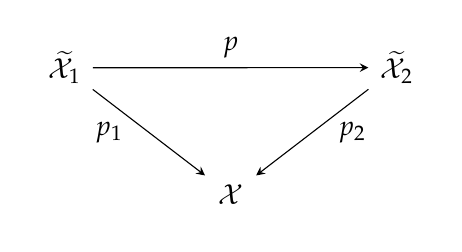
\begin{tikzpicture}
	\matrix (m) [matrix of math nodes,row sep=3em,column sep=4em,minimum width=2em]
	{
		\widetilde{\mathcal X}_1 & &\widetilde{\mathcal X}_2\\ 
		& {\mathcal X}\\};
	\path[-stealth]
	(m-1-1) edge node [above] {$p$} (m-1-3)
	(m-1-1) edge node [left]  {$p_1~~$} (m-2-2)
	(m-1-3) edge node [right] {$~~p_2$} (m-2-2);
	\end{tikzpicture}
	\\
	Suppose  $\sX$ is a  locally compact, locally connected,  Hausdorff space and $p_1$, $p_2$ are coverings. For all $g\in G\left( \left.\mathcal{\widetilde{X}}_1~\right|\mathcal{X}\right)$ the following condition holds
$$
\exists  \widetilde x_1 \in \widetilde\sX_1 \quad p \circ g\left( \widetilde x_1\right)  = p\left( \widetilde x_1\right)  \quad  \Leftrightarrow\quad \forall   \widetilde x_1 \in \widetilde\sX_1 \quad p \circ g\left( \widetilde x_1\right)= p\left( \widetilde x_1\right) . 
$$
\end{lemma}
\begin{proof}
	The implication $\Leftarrow$ is evident. Suppose that $\exists  \widetilde x_1 \in \widetilde\sX_1 \quad p\left(  g\widetilde x_1\right) \neq p\left( \widetilde x_1\right) $. There are open neighborhoods $\widetilde\sU'_2$ and $\widetilde\sU''_2$ of $p\left( \widetilde x_1\right) $ and $p\left( \widetilde gx_1\right)$ such that $\widetilde\sU'_2\cap \widetilde\sU''_2 = \emptyset$. Otherwise there is open neighborhood $\widetilde\sV_1$ of $\widetilde x_1$ such that $p\left( g\widetilde\sV_1\right)  \subset \widetilde\sU''_2$. It follows that $p\left(  g\widetilde y_1\right) \neq p\left( \widetilde y_1\right)$ for all $\widetilde y \in \widetilde \sU'_1\cap \widetilde\sV_1$. Hence the set
	$$
	\left\{\left.\widetilde y_1 \in \widetilde \sX_1~\right| p\left(  g\widetilde y_1\right) \neq p\left( \widetilde y_1\right)\right\}
	$$
	is open, or equivalently the set
	$$
	\widetilde{ \mathcal W}_1	=	\left\{\left.\widetilde y_1 \in \widetilde \sX_1~\right| p\left(  g\widetilde y_1\right) = p\left( \widetilde y_1\right)\right\}
	$$
	is closed.  Suppose that $\widetilde x_1 \in \widetilde \sX_1$ is such that $\widetilde x_1 = g \widetilde x_1$. There is an  open neighborhood $\widetilde \sU'_1$ of $\widetilde x_1$ such that $\left.p_1\right|_{\widetilde\sU'_1}$ is injective. There is an open neighborhood $\widetilde \sU'_2$ of $p\left( \widetilde x_1\right) $ such that $\left.p_2\right|_{\widetilde\sU'_2}$ is injective. Since $\sX$ is locally connected there is a connected open neighborhood $\sU$ of $p_1\left(\widetilde x_1\right)$ such that $\sU\subset p_1\left(\widetilde \sU'_1\right)\cap p_2\left(\widetilde\sU'_2 \right)$. If $\widetilde\sU_1 = \widetilde\sU'_1
\cap p_1^{-1}\left(\sU\right)$ and  $\widetilde\sU_2 = \widetilde\sU'_2
\cap p_2^{-1}\left(\sU\right)$ then both $\left.p_1\right|_{\widetilde\sU_1}$ and $\left.p_2\right|_{\widetilde\sU_2}$ are injective and may be regarded as homeomorphisms from both $\widetilde\sU_1$ and $\widetilde\sU_2$ onto $\sU$. For any $\widetilde y_1 \in \widetilde\sU_1$ one has
$$
p\left(g \widetilde y_1 \right)= \left( \left.p_2\right|_{\widetilde\sU_2}\right)^{-1}\circ p_1\left(g\widetilde y_1 \right).
$$
On the other hand from $g \in  G\left( \left.\mathcal{\widetilde{X}}_1~\right|\mathcal{X}\right)$ it follows that  $p_1\left(g \widetilde y_1 \right) =  p_1\left( \widetilde y_1 \right)$, hence the following condition holds
$$
p\left(g \widetilde y_1 \right)= \left( \left.p_2\right|_{\widetilde\sU_2}\right)^{-1}\circ p_1\left( \widetilde y_1 \right)=  p\left( \widetilde y_1 \right).
$$
The above equation is true for all $\widetilde y_1 \in \widetilde\sU_1$ so the set 	$\widetilde{ \mathcal W}_1$ is open.
From $\exists  \widetilde x_1 \in \widetilde\sX_1 \quad p \circ g\left( \widetilde x_1\right)  = p\left( \widetilde x_1\right)$ it turns out that $\widetilde{ \mathcal W}_1 \neq \emptyset$ and taking into account that $\sX$ is connected we conclude that $\widetilde{ \mathcal W}_1 = \widetilde{ \mathcal X}_1$. It equivalently means that
	$$
\forall   \widetilde x_1 \in \widetilde\sX_1 \quad p \circ g\left( \widetilde x_1\right)=p\left( \widetilde x_1\right) .
	$$
\end{proof}

\begin{corollary}\label{top_covp_cat_cor}
Consider the situation of the Lemma \ref{top_covp_cat_lem}. If the map $p$ is surjective and the covering $p_1$ is transitive then map $p$ is a transitive covering.
\end{corollary}
\begin{proof}
	From the Corollary \ref{top_cov_cat_cor} it follows that $p$ is a covering. There is the natural homomorphic inclusion $G\left( \left.{\widetilde{\sX}}_1~\right|\widetilde{\sX}_2\right)\subset  G\left(\left. \widetilde{\sX}_1~\right|\mathcal{X}\right)$. Let $\widetilde x_2 \in\widetilde \sX_2$ be a point and $x = p_2\left( \widetilde x_2\right)$. If $\widetilde x_1\in \widetilde\sX_1$ is such that $p\left(\widetilde x_1\right)= \widetilde x_2$ then $p_1^{-1}\left( x \right) = G\left( \left.\mathcal{\widetilde{X}}_1~\right|\mathcal{X}\right)\widetilde x_1$ because the covering $\widetilde p_1$ is transitive. It follows that $p^{-1}\left(\widetilde x_2 \right) = G_{\widetilde x_2}\widetilde x_1$ where
	$$
	G_{\widetilde x_2} = \left\{\left.g \in G\left( \left.\mathcal{\widetilde{X}}_1~\right|\mathcal{X}\right)\right| p\left(g \widetilde x_2 \right)=p\left( \widetilde x_2\right)  \right\}.
	$$
However from the Lemma 	\ref{top_covp_cat_lem} it follows that $G_{\widetilde x_2} = G\left( \left.{\widetilde{\sX}}_1~\right|\widetilde{\sX}_2\right)$, hence $p^{-1}\left(\widetilde x_2 \right) = G\left( \left.{\widetilde{\sX}}_1~\right|\widetilde{\sX}_2\right)\widetilde x_1$. 
 \end{proof}
\begin{definition}\label{top_gen_path_defn}
Let $\sX$ be a connected, locally connected, locally compact, Hausdorff space.
Let $\left\{\sU_\a\right\}_{\a \in \mathscr A}$ be a finite or countable family of connected open subsets of $\sX$, such that $\sX = \cup~ \sU_\a$ and for all $\a$ the closure of $\sU_\a$ is compact. An ordered finite subset $\left(\sU_{\a_1},...,\sU_{\a_n}\right)$ of the family $\left\{\sU_\a\right\}$ is said to be an  $\left\{\sU_\a\right\}$-\textit{path} if  $\sU_{\a_j}\cap \sU_{\a_{j+1}}\neq \emptyset$ for all $j = 1,...,n-1$ 
\end{definition}
\begin{lemma}\label{top_gen_path_lem}
Consider the situation of the Definition \ref{top_gen_path_defn}. If the space $\sX$ is Lindel\"{o}f then for any $\sU_{\a'}, \sU_{\a''} \in \sX$ there is a $\left\{\sU_\a\right\}$-{path} $\left(\sU_{\a_1},...,\sU_{\a_n}\right)$ such that $\sU_{\a_1}=\sU_{\a'}$ and $\sU_{\a_n}=\sU_{\a''}$ .
\end{lemma}
\begin{proof}
If $x' \in \sU_{\a'}$ and $x'' \in \sU_{\a''}$ then from the Lemma 	\ref{fin_comp_lin_lem} it follows that there is the sequence of connected compact sets $\left\{\sU_j\right\}_{j \in \N}$ such that $x' \in \sU_1$ and $\sX = \cup~\sU_j$. Let $n \in \N$ be such that $x'' \in \sU_n$ and $x'' \notin \sU_{n-1}$. From the proof of the Lemma  \ref{fin_comp_lin_lem} it turns out that there is a path $\left(\sU_{\a'_1},...,\sU_{\a'_k}\right)$ such that $x'$ lies in the closure of $\sU_{\a_1}$ and $x''$ lies in the closure of $\sU_{\a_k}$ The path $\left\{\sU_\a\right\}$-{path} $\left(\sU_{\a'}, \sU_{\a'_1},...,\sU_{\a'_k }, \sU_{\a''}\right)$ satisfies to this lemma.
\end{proof}
\begin{definition}\label{top_path_comp_defn}
If both $\mathfrak p'=\left(\sU_{\a'_1},...,\sU_{\a'_k}\right)$ and $\mathfrak p''=\left(\sU_{\a''_1},...,\sU_{\a''_l}\right)$ are paths such that $\sU_{\a'_k} = \sU_{\a''_1}$ then the path $\mathfrak p=\left(\sU_{\a'_1},...,\sU_{\a'_k},\sU_{\a''_2},...,\sU_{\a''_l} \right)$  is said to be the \textit{composition} of $\mathfrak p'$ and $\mathfrak p''$. We write
\be\label{top_path_comp_eqn}
\mathfrak p'\circ \mathfrak p''\bydef\mathfrak p.
\ee
\end{definition}
\begin{empt}\label{top_lconn_part}
	Let $\sX$ be a connected, locally connected, second-countable, locally compact Hausdorff space. Let $p: \widetilde{   \mathcal X }\to \sX$ is a transitive covering such that $G\left(\left.\widetilde{\sX}~\right|\sX\right)$ is countable. There is a countable set $\left\{\sU_\a\right\}_{\a \in \mathscr A}$  set of open connected subsets of $\sX$ such that following conditions hold:
	\begin{itemize}
		\item $\sX = \cup_{\a \in \mathscr A} \sU_\a$.
		\item The closure of $\sU_{\a}$ is a compact set for all $\a \in \mathscr A$.
		\item $\sU_\a$ is evenly covered by $p$.
		\item The family $\left\{\sU_\a\right\}$ is locally finite (cf. Definition \ref{top_loc_fin_defn}).
	\end{itemize}
	From the Theorem \ref{top_part_u_thm}  it turns out that there is a partition of unity $\sum_{\a \in \mathscr A}a_\a\left(x\right)=1$ subordinated $\left\{\sU_\a\right\}_{\a \in \mathscr A}$. Consider the situation \ref{top_lconn_part}. For any $\a \in \mathscr A$ we select an open connected set $\widetilde \sU_\a \in \widetilde\sX$. The family $\left\{g \widetilde \sU_\a\right\}_{\left(g, \a\right)\in  G\left(\left.\widetilde{\sX}~\right|\sX\right)\times \mathscr A}$ is locally finite and 
	$$
	\widetilde \sX=\bigcup_{\left(g, \a\right)\in  G\left(\left.\widetilde{\sX}~\right|\sX\right)\times \mathscr A} 	g \widetilde \sU_\a
	$$
\end{empt}
\begin{definition}\label{top_lconn_defn}
	In the above situation we say that the family $\left\{\sU_\a\right\}_{\a \in \mathscr A}$ is \textit{compliant with} $p$, and the family
	$\left\{g \widetilde \sU_\a\right\}_{\left(g, \a\right)\in  G\left(\left.\widetilde{\sX}~\right|\sX\right)\times \mathscr A}$ is the $p$-\textit{lift} of $\left\{\sU_\a\right\}_{\a \in \mathscr A}$.
\end{definition}
\begin{remark}\label{top_lconn_rem}
	Sometimes we denote by $\widetilde{ \mathscr A}\bydef G\left(\left.\widetilde{\sX}~\right|\sX\right)\times \mathscr A$ and
	\be\label{top_lconn_eqn}	
	\left\{\widetilde \sU_{\widetilde \a }\right\}_{\widetilde{ \a}\in \widetilde{ \mathscr A}}\bydef \left\{g \widetilde \sU_\a\right\}_{\left(g, \a\right)\in  G\left(\left.\widetilde{\sX}~\right|\sX\right)\times \mathscr A}.
	\ee
\end{remark}

\begin{empt}\label{top_path_lift_empt}
Let $\sX$ be a connected, locally connected,  second-countable, Hausdorff space, and let  $p: \widetilde{   \mathcal X }\to \sX$ be a transitive covering, such that $\widetilde{   \mathcal X }$ is connected. Consider a described in \ref{top_lconn_part} family $\left\{\sU_\a\right\}_{\a \in \mathscr A}$ of open subsets of $\sX$. Denote by $\left\{\widetilde \sU_{\widetilde \a }\right\}_{\widetilde{ \a}\in \widetilde{\mathscr A}}~$ the $p$-lift of $\left\{\sU_\a\right\}_{\a \in \mathscr A}$ (cf. Definition \ref{top_lconn_defn} and Equation \eqref{top_lconn_eqn}).
\end{empt}
\begin{definition}\label{top_path_desc_defn}
Consider the situation \ref{top_path_lift_empt}.  If $\widetilde{\mathfrak p}=\left(\widetilde\sU_{\widetilde\a_1},...,\widetilde\sU_{\widetilde\a_n}\right)$ is a $\left\{\widetilde \sU_{\widetilde \a }\right\}$-path  then clearly $\mathfrak p=\left(p\left( \widetilde\sU_{\widetilde\a_1}\right) ,...,p\left( \sU_{\widetilde\a_n}\right) \right)$ is a $\left\{\sU_\a\right\}$-path. We say that ${\mathfrak p}$ is the $p$-\textit{descend} of $\widetilde{\mathfrak p}$ and we write
\be\label{top_path_desc_eqn}
{\mathfrak p}\bydef\desc_p~\widetilde{\mathfrak p}.
\ee 
\end{definition}
\begin{lemma}\label{top_path_lift_lem}
	If ${\mathfrak p}=\left(\sU_{\a_1},...,\sU_{\a_n}\right)$ is a  $\left\{\sU_\a\right\}$-{path}  then for any $\widetilde \sU_{\widetilde \a' }\in \left\{\widetilde \sU_{\widetilde \a }\right\}$ such that $p\left(\widetilde \sU_{\widetilde \a' } \right) = \sU_{\a_1}$ there is the unique  $\left\{\widetilde \sU_{\widetilde \a }\right\}$-path $\widetilde{\mathfrak p}$ such that ${\mathfrak p}=\desc_p~\widetilde{\mathfrak p}$ and the first element of $\widetilde{\mathfrak p}$ is $\widetilde \sU_{\widetilde \a' }$.
\end{lemma}
\begin{proof}
From the condition of this lemma the first element of $\widetilde{\mathfrak p}$ is $\widetilde \sU_{\widetilde \a' }$, other elements will be constructed by the induction.
 Suppose that we already have $j$ elements $\widetilde\sU_{\widetilde\a_1},...,\widetilde\sU_{\widetilde\a_j}$ of the path $\widetilde{\mathfrak p}$. If $\widetilde\sU' \in \left\{\widetilde \sU_{\widetilde \a }\right\}$ is such that $p\left( \widetilde\sU'\right) = \sU_{\a_{j+1}}$ then from $\sU_{\a_j}\cap \sU_{\a_{j+1}}\neq \emptyset$ it turns out that there is the unique $g \in G\left(\left.\widetilde{   \mathcal X }~\right|{   \mathcal X } \right)$ such that $g\widetilde\sU'\cap \widetilde\sU_{\widetilde\a_j}\neq\emptyset$. We set $g\widetilde\sU'$ as $j+1^{\text{th}}$ element of $\widetilde{\mathfrak p}$, i.e. $\sU_{\widetilde\a_{j+1}}\bydef g\widetilde\sU'$.  In result the path
$$
\widetilde{\mathfrak p} \bydef \left(\widetilde\sU_{\widetilde\a_1},...,\sU_{\widetilde\a_n}\right)
$$
satisfies to the requirements of this lemma. The above  construction is unique so $\widetilde{\mathfrak p}$ is uniquely defined by the conditions of this lemma.
\end{proof}
\begin{definition}\label{top_path_lift_defn}
The given by the Lemma \ref{top_path_lift_lem} path $\widetilde{\mathfrak p}$ is said to be the $p$-$\sU_{\widetilde \a' }$-\textit{lift} of $\mathfrak p$. We write
\be\label{top_path_lift_eqn}
\lift_p^{\sU_{\widetilde \a' }}~\mathfrak p\bydef\widetilde{\mathfrak p}.
\ee 
\end{definition}
\begin{empt}\label{top_path_comp_empt}
In the situation \ref{top_path_lift_empt} select $\widetilde x_0\in \widetilde \sX$ and $\widetilde\sU_0 \in \left\{\widetilde \sU_{\widetilde \a }\right\}$ is such that $\widetilde x_0\in \widetilde\sU_0$. Let $\sU_0 = p\left(\widetilde\sU_0 \right)$ and $x_0 = p\left(\widetilde x_0 \right)$. From the Lemma \ref{top_gen_path_lem} it follows that for all $g \in G\left(\left.\widetilde{   \mathcal X }~\right|{   \mathcal X } \right)$ there is a $\left\{\widetilde \sU_{\widetilde \a }\right\}$ path $\widetilde{\mathfrak p}_g=\left(\widetilde\sU_{\widetilde\a_1},...,\widetilde\sU_{\widetilde\a_n}\right)$ such that
\be\label{top_path_compl_eqn}
\widetilde\sU_{\widetilde\a_1}= \widetilde\sU_{0}; \quad \widetilde\sU_{\widetilde\a_n}= g \widetilde\sU_{0}
\ee
A path which satisfies to  \eqref{top_path_compl_eqn} is not unique. One has
\be\label{top_path_comp_lem_eqn}
\begin{split}
{\mathfrak p}_g= \desc_p \widetilde{\mathfrak p}_g \quad \Leftrightarrow \quad p\left(  {\mathfrak p}_g\right)  =p\left( \mathfrak p\right) =\left(p\left( \widetilde\sU_{\widetilde\a_1}\right) ,...,p\left( \sU_{\widetilde\a_n}\right) \right)\quad \Rightarrow
\\
\Rightarrow p\left( \widetilde\sU_{\widetilde\a_1}\right)= p\left( \widetilde\sU_{\widetilde\a_n}\right)= \sU_0.
\end{split}
\ee
If $g', g'' \in G\left(\left.\widetilde{   \mathcal X }~\right|{   \mathcal X } \right)$ then from \eqref{top_path_comp_lem_eqn} it follows that there is the composition $\desc_p \widetilde{\mathfrak p}_{g'}\circ \desc_p \widetilde{\mathfrak p}_{g''}$ (cf. Definition \ref{top_path_comp_defn}).
\end{empt}
\begin{definition}\label{top_path_corr_defn}
	In the situation  \ref{top_path_comp_empt} we say that the path $\widetilde{\mathfrak p}_g$ \textit{corresponds to} $g \in G\left(\left.\widetilde{   \mathcal X }~\right|{   \mathcal X } \right)$. This path is not unique.
\end{definition}

\begin{lemma}\label{top_lift_comp_lem}
If we consider the situation \ref{top_path_comp_empt} and suppose that $\widetilde{\mathfrak p}_{g'} = \left( \widetilde\sU_{\widetilde\a'_1},..., \widetilde\sU_{\widetilde\a'_k}\right)$, $\widetilde{\mathfrak p}_{g''} = \left( \widetilde\sU_{\widetilde\a''_1},..., \widetilde\sU_{\widetilde\a''_l}\right)$. If
\bean
\widetilde{\mathfrak p} = \lift^{\widetilde\sU_0}_p\left( \desc_p \widetilde{\mathfrak p}_{g'}\circ \desc_p \widetilde{\mathfrak p}_{g''}\right),\\ 
\widetilde{\mathfrak p}= \left( \widetilde\sU_{\widetilde\a_1},..., \widetilde\sU_{\widetilde\a_{k + l -1}}\right)
\eean
then $ \widetilde\sU_{\widetilde\a_{k + l -1}}= g'g''\widetilde \sU_0$.
\end{lemma}
\begin{proof}
From $\widetilde\sU_{\widetilde\a'_k}= g' \widetilde\sU_0$ it follows that
$$
\widetilde{\mathfrak p} = \left( \widetilde\sU_{\widetilde\a'_1},..., \widetilde\sU_{\widetilde\a'_k}, g'\widetilde\sU_{\widetilde\a''_2},..., g'\widetilde\sU_{\widetilde\a''_l}\right)
$$
and taking into account $\widetilde\sU_{\widetilde\a''_l}= g' \widetilde\sU_0$ one has $ \widetilde\sU_{\widetilde\a_{k + l -1}}=\widetilde\sU_{\widetilde\a''_k}= g'g''\widetilde \sU_0$.
\end{proof}
\begin{empt}\label{top_g_homo_empt}
In the situation  \ref{top_path_comp_empt}	consider a commutative triangle of connected topological spaces and  transitive coverings.
\newline
\begin{tikzpicture}
\matrix (m) [matrix of math nodes,row sep=3em,column sep=4em,minimum width=2em]
{
	\widetilde{\mathcal X}' & &\widetilde{\mathcal X}''\\ 
	& {\mathcal X}\\};
\path[-stealth]
(m-1-1) edge node [above] {$p$} (m-1-3)
(m-1-1) edge node [left]  {$p'~~$} (m-2-2)
(m-1-3) edge node [right] {$~~p''$} (m-2-2);
\end{tikzpicture}
\\
Suppose that $\sX$ is a connected, locally connected, locally compact, Hausdorff space. Consider a described in \ref{top_lconn_part} family $\left\{\sU_\a\right\}_{\a \in \mathscr A}$ of open subsets of $\sX$. Let both  $\left\{\widetilde \sU_{\widetilde \a' }\right\}_{\widetilde{ \a'}\in \widetilde{\mathscr A}'}~$, $\left\{\widetilde \sU_{\widetilde \a'' }\right\}_{\widetilde{ \a''}\in \widetilde{\mathscr A}''}~$ be the  $p'$-lift and $p''$-lift of $\left\{\sU_\a\right\}_{\a \in \mathscr A}$ respectively (cf. Definition \ref{top_lconn_defn} and Equation \eqref{top_lconn_eqn}). Let $\widetilde \sU'_0 \in \left\{\widetilde \sU_{\widetilde \a' }\right\}$, and $\widetilde x_0 \in \widetilde \sU'_0$. Denote by $ \widetilde \sU''_0\bydef p\left(\widetilde \sU'_0\right)\subset \widetilde \sX''$, $  \sU_0\bydef p'\left(\widetilde \sU'_0\right)\subset \sX$, $\widetilde x''_0\bydef p\left(\widetilde x'_0\right)\subset \widetilde \sU''_0$, $  x_0\bydef p'\left(\widetilde x'_0\right)\subset \sU_0$. Both $p'$ and $p''$ are transitive coverings, hence from the Corollary \ref{top_trans_tp_cov_cor} it follows that there are bijecive maps
 	\bean 
 G\left(\widetilde{   \mathcal X }'~|~{   \mathcal X } \right)\xrightarrow{\approx}p'^{-1}p'\left(\widetilde x'_0 \right),\\
 g \mapsto g\widetilde x'_0;\\
 G\left(\widetilde{   \mathcal X }''~|~{   \mathcal X } \right)\xrightarrow{\approx}p''^{-1}p''\left(\widetilde x''_0 \right),\\
 g \mapsto g\widetilde x''_0. 
 \eean
 On the other hand the map $p$ induces the surjective map $p'^{-1}p'\left(\widetilde x'_0 \right)\to p''^{-1}p''\left(\widetilde x''_0 \right)$ so one has the surjecive map
 \be\label{top_g_homo_eqn}
 h :  G\left(\widetilde{   \mathcal X }'~|~{   \mathcal X } \right)\to G\left(\widetilde{   \mathcal X }''~|~{   \mathcal X } \right)
 \ee
\end{empt}
\begin{lemma}\label{top_homo_lem}
In the situation \ref{top_g_homo_empt} following condition holds:
\begin{itemize}
	\item [(i)] 	The given by \eqref{top_g_homo_eqn} surjective map $ h :  G\left(\widetilde{   \mathcal X }'~|~{   \mathcal X } \right)\to G\left(\widetilde{   \mathcal X }''~|~{   \mathcal X } \right)$ is a homomorphism of groups.
	\item[(ii)] If we consider the natural inclusion $ G\left(\widetilde{   \mathcal X }'~|~{   \mathcal X }'' \right)\subset  G\left(\widetilde{   \mathcal X }'~|~{   \mathcal X } \right)$ then $ G\left(\widetilde{   \mathcal X }'~|~{   \mathcal X }'' \right)$ is a normal subgroup of $ G\left(\widetilde{   \mathcal X }'~|~{   \mathcal X } \right)$ (cf. Definition \ref{normal_subgroup_defn}).
\end{itemize}
\end{lemma}
\begin{proof} (i)
Let $g'_1, g'_2 \in G\left(\widetilde{   \mathcal X }'~|~{   \mathcal X } \right)$ and let both $\widetilde{\mathfrak p}'_{g'_1}= \left( \widetilde\sU'_{\widetilde\a'_{1,1}},..., \widetilde\sU'_{\widetilde\a'_{1, k}}\right)$, $\widetilde{\mathfrak p}'_{g'_2}= \left( \widetilde\sU'_{\widetilde\a'_{2,1}},..., \widetilde\sU'_{\widetilde\a'_{2, l}}\right)$ are $\left\{\widetilde \sU'_{\widetilde \a' }\right\}$-paths which correspond to  $g'_1$ and $g'_2$ respectively (cf. Definition \ref{top_path_corr_defn}). Clearly both $\desc_p\widetilde{\mathfrak p}'_{g'_1}$ and $\desc_p \widetilde{\mathfrak p}'_{g'_2}$ are $\left\{\widetilde \sU_{\widetilde \a'' }\right\}$-paths which correspond to  $h\left( g_1\right) $ and $h\left( g_2\right)$ respectively. From the Lemma  \ref{top_lift_comp_lem} it follows that both 
\bean
\widetilde{\mathfrak p}' \bydef \lift^{\widetilde\sU'_0}_{p'}\left( \desc_{p'} \widetilde{\mathfrak p}_{g_1}\circ \desc_{p'} \widetilde{\mathfrak p}_{g_2}\right),\\
\widetilde{\mathfrak p}''\bydef \lift^{\widetilde\sU''_0}_{p''}\left( \desc_{p'} \widetilde{\mathfrak p}_{g_1}\circ \desc_{p'} \widetilde{\mathfrak p}_{g_2}\right)
\eean
are $\left\{\widetilde \sU'_{\widetilde \a' }\right\}$ and $\left\{\widetilde \sU''_{\widetilde \a'' }\right\}$-paths which correspond to $g_1 g_2$ and $h\left( g_1\right)h\left( g_2\right)$ respectively. It means that that   $\widetilde{\mathfrak p}'= \left( \widetilde\sU'_{\widetilde\a'_{1}},..., \widetilde\sU'_{\widetilde\a'_{k + l -1}}\right)$ then $\widetilde\sU'_{\widetilde\a'_{k + l -1}}= g_1g_2\widetilde \sU'_0$. On the other hand  $\widetilde{\mathfrak p}''= \desc_p \widetilde{\mathfrak p}'= \left( p\left( \widetilde\sU'_{\widetilde\a'_{1}}\right) ,..., p\left( \widetilde\sU'_{\widetilde\a'_{k + l -1}}\right) \right)$, so $p\left( \widetilde\sU'_{\widetilde\a'_{k + l -1}}\right)= h\left(g_1g_2 \right) \widetilde\sU''_0$, i.e. $\widetilde{\mathfrak p}''$ corresponds to $h\left(g_1g_2 \right)$. It follows that $h\left(g_1g_2 \right)=h\left(g_1 \right)h\left(g_2 \right)$, i.e. $h$ is a homomorphism.\\
(ii) Follows from $G\left(\widetilde{   \mathcal X }''~|~{   \mathcal X }' \right)= \ker h$.
\end{proof}




\begin{corollary}\label{com_norm_cor}
	Let $\sX$, $\sX'$ and $\sX''$ be connected, locally connected,  second-countable, locally compact, Hausdorff spaces.
	If $p': \sX' \to \sX$ and $p'': \sX'' \to \sX'$ are finite-fold  transitive  coverings such that $p'' \circ p'$ is transitive then
	\begin{enumerate}
		\item[(i)] There is an exact sequence of group homomorphisms
		$$
		\left\{e\right\} \to 	G\left(\left.\sX''~\right|~\sX' \right) \to 	G\left(\left.\sX''~\right|~\sX \right) \to 	G\left(\sX'~|~\sX \right) \to \left\{e\right\}.
		$$
		\item[(ii)]
		For any $g \in 	G\left(\left.\sX''~\right|~\sX \right)$ one has
		$
		gC_0\left(\sX' \right) = C_0\left(\sX' \right). 
		$
	\end{enumerate}
\end{corollary}
\begin{proof}
	(i) Directly follows from the Lemma \ref{top_homo_lem}.\\
	(ii) Suppose  $a' \in C_0\left(\sX'' \right)$. One has $a' \in C_0\left(\sX'\right)$ if and only if $g''a' = a'$ for all $g'' \in G\left(\left.\sX''~\right|~\sX' \right)$. Since 	$G\left(\left.\sX''~\right|~\sX' \right)$ is a normal subgroup of $G\left(\left.\sX''~\right|~\sX \right)$ for each $g \in  G\left(\left.\sX''~\right|~\sX \right)$ and $g''_1 \in  G\left(\left.\sX''~\right|~\sX' \right)$ there is $g''_2 \in  G\left(\left.\sX''~\right|~\sX' \right)$ such that $g''_1g = gg''_2$, it turns out $g''_1ga' = gg''_2a'= ga'$, i.e. $g''_1 \left(ga' \right)= ga'$ so one has $ga' \in   C_0\left(\sX' \right)$.
\end{proof}


\begin{definition}\label{top_fin_cov_defn}
	Let $\sX$ be a connected, locally connected,  locally compact, second-countable, Hausdorff space. Let us consider the  category $\mathfrak{FinCov}$-$\sX$ such that
	\begin{itemize}
		\item Objects of  $\mathfrak{FinCov}$-$\sX$ are transitive finite-fold coverings $\widetilde\sX \to \sX$ of $\sX$ where the space $\widetilde\sX$ is connected.
		\item A morphism form $p_1:\widetilde\sX_1 \to \sX$ to $p_2:\widetilde\sX_2 \to \sX$ is a surjective continuous map $p_{12}: \widetilde\sX_1 \to \widetilde\sX_2$ such that $p_{12} \circ p_2 = p_1$.
	\end{itemize}
	We say that $\mathfrak{FinCov}$-$\sX$ is the \textit{finite covering category} of $\sX$.	
\end{definition}
\begin{remark}\label{top_fin_cov_tr_rem}
	From the Corollary \ref{top_covp_cat_cor} it follows that $p_{12}$ is a transitive covering.
\end{remark}

\begin{remark}\label{top_fin_cov_rem}
	We also use the alternative notation in which objects of $\mathfrak{FinCov}$-$\sX$ are covering spaces, i.e. a covering $\widetilde\sX \to \sX$ is replaced with the space $\widetilde\sX$.
\end{remark}
\begin{lemma}\label{top_compliant_covering_lem}
	If $p_1:\widetilde\sX_1 \to \sX$, $p_2:\widetilde\sX_2 \to \sX$ are objects of $\mathfrak{FinCov}$-$\sX$ and $p': \widetilde\sX_1 \to  \widetilde\sX_2$, $p'': \widetilde\sX_1 \to  \widetilde\sX_2$ are morphisms of $\mathfrak{FinCov}$-$\sX$ then there is $g \in 	G\left(\left.\widetilde\sX_2~\right|\sX\right)$ such that
	$$
	p'' =  g \circ p'.
	$$
\end{lemma}
\begin{proof}
	The covering $p_2$ is transitive, so from $p' \circ p_2= p'' \circ p_2$ it turns out that
	$$
\forall	\widetilde x_1\in \widetilde\sX_1\quad  \text{ there is the unique } g_{\widetilde x_1} \in G\left(\left.\widetilde\sX_2~\right|\sX\right)\quad p'\left( \widetilde x_1\right)= g_{\widetilde x_1} \circ p''\left(\widetilde x_1 \right).  
	$$
	There is the map
\bean
	h: \widetilde\sX_1 \to G\left(\left.\widetilde\sX_2~\right|\sX\right);\\
\widetilde x_1\mapsto g_{\widetilde x_1} 
\eean
and since both $p'$ and $p''$ are local isomorphisms the map $h$ is continuous. However the space  $G\left(\left.\widetilde\sX_2~\right|\sX\right)$ of homeomorphisms is discrete and the space $\widetilde\sX_1$ is connected, hence the map $h$ is constant, i.e.
$$
\exists g \in G\left(\left.\widetilde\sX_2~\right|\sX\right) \quad \forall \widetilde x_1\in \widetilde\sX_1 \quad p''\left( \widetilde x_1\right) = g\circ p'\left( \widetilde x_1\right).
$$
\end{proof} 

\begin{definition}\label{top_pointed_defn}
	If $\sX$ is a set (resp. topological space) and $x_0 \in \sX$ is a base-point then we say that the pair $\left(\sX, x_0 \right)$ is a \textit{pointed set} (resp. \textit{pointed space}). If both $\left(\sX, x_0 \right)$ and $\left(\sY, y_0 \right)$ are pointed spaces and $\varphi: \sX \to \sY$ is such that $\varphi\left(x_0\right)= y_0$ then we say that $\varphi$ is a \textit{pointed map}. We write
	\be\label{top_pointed_eqn}
	\varphi: \left(\sX, x_0 \right)\to\left(\sY, y_0 \right)
	\ee
\end{definition}
\begin{definition}\label{top_fin_cov_p_defn}
	Let $\left(\sX, x_0 \right)$ be a pointed space such that $\sX$ is a connected, locally connected,  locally compact, second-countable, Hausdorff space. Let us consider the  category $\mathfrak{FinCov}$-$\left( \sX, x_0\right) $ such that
	\begin{itemize}
		\item Objects of  $\mathfrak{FinCov}$-$\left( \sX, x_0\right)$ are transitive finite-fold coverings\\ $\left( \widetilde\sX, \widetilde x_0\right)  \to \left( \sX, x_0\right)$ of $\sX$ preserving base-points.
		\item A morphism form $p_1:\left( \widetilde\sX_1, \widetilde x^1_0\right)\to \left( \sX, x_0\right)$ to $p_2:\left( \widetilde\sX_2, \widetilde x^2_0\right)\to \left( \sX, x_0\right)$ is a preserving base-points surjective continuous map $p: \left( \widetilde\sX_1, \widetilde x^1_0\right)\to \left( \sX_2, x^2_0\right)$ such that $p \circ p_1 = p_2$.
	\end{itemize}
	We say that $\mathfrak{FinCov}$-$\left( \sX, x_0\right)$ is the \textit{topological pointed finite covering category} of $\left( \sX, x_0\right)$.  
\end{definition}
\begin{remark}
	The category $\mathfrak{FinCov}$-$\left( \sX, x_0\right)$ is a subcategory of  $\mathfrak{FinCov}$-$\sX$.
\end{remark}
\begin{remark}
	If both $p_1:\left( \widetilde\sX_1, \widetilde x^1_0\right)\to \left( \sX, x_0\right)$ and  $p_2:\left( \widetilde\sX_2, \widetilde x^2_0\right)\to \left( \sX, x_0\right)$ are objects of $\mathfrak{FinCov}$-$\left( \sX, x_0\right)$ then there is no more than one morphism from $p_1$ to $p_2$.
\end{remark}



\begin{lemma}\label{top_fin_comp_lin_cov_lem}
	Let $\mathcal X$ be a connected, locally connected,  locally compact, Hausdorff, Lindel\"{o}f space. Suppose that  $\widetilde{\mathcal X}\to \sX$ be a transitive finite-fold covering.   Then for any $x_0 \in \mathcal X$ there is  a  finite or countable sequence $\sU_1 \subsetneqq  ...\subsetneqq \sU_n\subsetneqq ...$ of connected open subsets of $\sX$ such that
	\begin{enumerate}
		\item[(i)] $x_0 \in \sU_1$.
		\item[(ii)]  For any $n \in \N$ the closure of $\sU_n$ is compact.
		\item[(iii)] $\cup~ \sU_n = \sX$.
		\item[(iv)] The space $p^{-1}\left( \sU_n\right)$ is connected for any $n \in \N$.
		\end{enumerate}  
\end{lemma}
\begin{proof}
	(i)-(iii) From the Lemma \ref{fin_comp_lin_lem} it follows that there is a  finite or countable sequence $\sU_1 \subsetneqq  ...\subsetneqq \sU_n\subsetneqq ...$ of connected open subsets of $\sX$ such that conditions (i)-(iii) holds.\\
	(iv)
	Let $\widetilde x_0 \in p^{-1}\left( \sU_n\right)$ be any point, and let $\widetilde \sU^{\widetilde x_0}_n$ be a connected component of $p^{-1}\left( \sU_n\right)$ such that $\widetilde x_0\in \widetilde \sU^{\widetilde x_0}_n$. If $G_n = \left\{\left.g\in G\left( \widetilde{   \mathcal X }~|~\sX\right)\right| g   \widetilde x_0\in \sU^{\widetilde x_0}_n\right\}$ then there is  
	is a nondecreasing sequence of  subgroups
	$$
	G_1 \subseteq ... \subseteq G_n \subseteq ...
	$$
	Since $G\left( \widetilde{   \mathcal X }~|~\sX\right)$ is finite there is $m \in \N$ such that $G_k = G_m$ for every $k \ge m$. If $J \in G\left( \widetilde{   \mathcal X }~|~\sX\right)$ is a set of representatives of $G\left( \widetilde{   \mathcal X }~|~\sX\right)/G_m$ and  $\widetilde\sU^{\widetilde x_0}= \cup_{n \in \N} \widetilde\sU^{\widetilde x_0}_n$ then one has
	$$
	\widetilde\sX = \bigcup_{n \in \N}p^{-1}\left(\sU_n \right) = \bigsqcup_{g \in J}g \widetilde\sU^{\widetilde x_0}
	$$
	Since the space $\widetilde\sX$ is connected the set $J$ is a singleton. It follows that $p^{-1}\left(\sU_k \right)= \widetilde\sU^{\widetilde x_0}_k$ for every $k \ge m$ i.e. $p^{-1}\left(\sU_k \right)$ is connected. So the finite or countable subsequence $\sU_m \subsetneqq  ...\subsetneqq \sU_k\subsetneqq ...$ of $\sU_1 \subsetneqq  ...\subsetneqq \sU_n\subsetneqq ...$ satisfies to the condition (iv).\\
\end{proof}

\begin{lemma}\label{top_conn_cov_lem}
	Let $\sX$ be a  connected, locally connected, locally compact, Hausdorff space, and let $\sU \subset \sX$ be a connected open subspace. If $p:	\widetilde{   \mathcal X } \to \mathcal X$ is a transitive covering, such that such that the space $\widetilde{\sU} = p^{-1}\left(\sU \right)$ is connected then the restriction $p|_{\widetilde{\sU}}: \widetilde{\sU}\to {\sU}$ is a transitive covering. Moreover  the map
	\be\label{top_res_iso_eqn}
	\begin{split}
	h:	G\left(\left. \widetilde{   \sX }~\right|\sX\right)\to G\left(\left. \widetilde{   \sU }~\right|\sU\right),\\
		g \mapsto g|_{\widetilde{\sU}}
	\end{split}
	\ee
	is the isomorphism of groups.
\end{lemma}
\begin{proof}
	The covering $p$ is transitive, hence if  $\widetilde x_0 \in \widetilde{   \mathcal U }$ then there is a bijection
	$$
G\left(\left. \widetilde{   \sX }~\right|\sX\right) \xrightarrow{\approx} p^{-1}\circ p\left( \widetilde x_0 \right) 
	$$
	it follows that the map \eqref{top_res_iso_eqn} is injective. If $g' \in G\left(\left. \widetilde{   \sU }~\right|\sU\right)$ then for any $\widetilde x \in \widetilde{   \mathcal U }$ there is $g_{\widetilde{   x}}\in G\left(\left. \widetilde{   \sX }~\right|\sX\right)$ such that $g'\widetilde x =  g_{\widetilde{   x}'} {\widetilde{   x}}$. There is a continuous map
	\bean
\widetilde{   \mathcal U } \to G\left(\left. \widetilde{   \sX }~\right|\sX\right);\\
{\widetilde{   x}} \mapsto g_{\widetilde{   x}'}.
	\eean
	Since $\widetilde{   \mathcal U }$ is connected and $G\left( \widetilde{   \mathcal X }~|~\sX\right)$ is a discrete group of homeomorphisms the map is constant, so that there is the unique $g \in G\left(\left. \widetilde{   \sX }~\right|\sX\right)$ such that $g' = g|_{\widetilde{\sU}}$, i.e. the map $h$ is surjecive.

\end{proof}




\section{Vector bundles and spaces of sections}
\paragraph*{} This section is not exclusively devoted to commutative $C^*$-algebras. It contains a more general theory, where $C^*$-algebras are represented by locally trivial  bundles. Homogeneous $C^*$ algebras and  with continuous trace $C^*$-algebras can be represented as locally trivial bundles. Any commutative $C^*$-algebra is also a vector bundle with one-dimensional fibers. So this theory is used in this chapter and the chapters \ref{ctr_chap}, \ref{vf_chap}, \ref{foliations_chap}. 
\begin{remark}\label{com_inf_rem}
	The section \ref{top_vb_sub_sub} describes the theory of vector bundles with  finite-dimensional fibers. However many results of the theory can be applied to  vector bundles where any fiber is a more general Banach space. Below the word \textit{vector bundle} means that a fiber may be arbitrary Banach space. 
\end{remark} 
\begin{empt}\label{top_bundle_sec_empt}
	Let $\sX$ be a locally compact Hausdorff space and   $\xi= \left( E, \pi, \mathcal X\right)$ is a vector bundle (cf. Definition \ref{top_vb_defn} and Remark \ref{com_inf_rem}) such that any fiber is a Banach $\C$-space. The space $\Ga\left( E, \pi, \mathcal X\right)$ of sections of $\left( E, \pi, \mathcal X\right)$ is a $\C$-space. For any $a \in \Ga\left( E, \pi, \mathcal X\right)$ the given by
	\be\label{top_normb_eqn}
	\begin{split}
		\text{norm}_a : \sX \to \R,\\
		x \mapsto \left\| a_x\right\| 
	\end{split}
	\ee
	map is continuous. Denote by
	\be\label{top_ub_eqn}
	\begin{split}
		\Ga_c\left( E, \pi, \mathcal X\right)\bydef \left\{\left.a \in \Ga\left( E, \pi, \mathcal X\right)\right| \text{norm}_a \in C_c\left(\sX\right) \right\},\\
		\Ga_0\left( E, \pi, \mathcal X\right)\bydef \left\{\left.a \in \Ga\left( E, \pi, \mathcal X\right)\right| \text{norm}_a \in C_0\left(\sX\right) \right\},\\
		\Ga_b\left( E, \pi, \mathcal X\right)\bydef\left\{\left.a \in \Ga\left( E, \pi, \mathcal X\right)\right| \text{norm}_a \in C_b\left(\sX\right) \right\}.\\
	\end{split}
	\ee
	There is the norm  $\left\|a\right\|\bydef\left\| \text{norm}_a\right\|$ on the above spaces such that both $\Ga_0\left( E, \pi, \mathcal X\right)$ and $\Ga_b\left( E, \pi, \mathcal X\right)$ are Banach spaces and $\Ga_c\left( E, \pi, \mathcal X\right)$ is dense in $\Ga_0\left( E, \pi, \mathcal X\right)$. If $f: \sY \to \sX$ is a continuous map and $\left(E\times_{\sX}\sY, \rho, \mathcal Y\right)$ is the {inverse image} of $\left( E, \pi, \mathcal X\right)$ by $f$ (cf. Definition \ref{vb_inv_img_funct_defn}) then the natural projection $E\times_{\sX}\sY\to E$ yields the natural $\C$-linear maps
	\be\label{top_uba_eqn}
	\begin{split}
		\Ga\left( E, \pi, \mathcal X\right)\hookto \Ga\left(E\times_{\sX}\sY, \rho, \mathcal Y\right),\\
		\Ga_b\left( E, \pi, \mathcal X\right)\hookto \Ga_b\left(E\times_{\sX}\sY, \rho, \mathcal Y\right)\\
	\end{split}
	\ee
	such that the second map is an isometry. Consider a category $\mathfrak{Top}$-$\sX$ such that
	\begin{itemize}
		\item Objects of are continuous maps $\sY \to \sX$.
		\item Morphism  $\sY' \to \sX$ to $\sY'' \to \sX$ is a continuous map $f: \sY' \to \sY''$ such that the following diagram
		\newline
		\begin{tikzpicture}
		\matrix (m) [matrix of math nodes,row sep=3em,column sep=4em,minimum width=2em]
		{
			{\mathcal Y'} & &{\mathcal Y''}\\ 
			& {\mathcal X}\\};
		\path[-stealth]
		(m-1-1) edge node [above] {$f$} (m-1-3)
		(m-1-1) edge node [left]  {} (m-2-2)
		(m-1-3) edge node [right] {} (m-2-2);
		\end{tikzpicture}
		\\
		is commutative.
	\end{itemize}
	For any vector bundle $\left( E, \pi, \mathcal X\right)$ equations \eqref{top_ub_eqn} and \eqref{top_uba_eqn} yield two contravariant functors $\Ga$ and $\Ga_b$ form  $\mathfrak{Top}$-$\sX$ to the category of vector spaces given such that 
	\be\label{top_f_eqn}
	\begin{split}
		\Ga\left(\sY \right) \bydef  \Ga\left(E\times_{\sX}\sY, \rho, \mathcal Y\right),\\
		\Ga_b\left(\sY \right) \bydef  \Ga_b\left(E\times_{\sX}\sY, \rho, \mathcal Y\right),\\
		\Ga\left(f \right)\bydef \left(\Ga\left(E\times_{\sX}\sY'', \rho, \mathcal Y''\right)\to \Ga\left(E\times_{\sX}\sY', \rho, \mathcal Y'\right) \right),
		\\
		\Ga_b\left(f \right)\bydef \left(\Ga_b\left(E\times_{\sX}\sY'', \rho, \mathcal Y''\right)\to \Ga_b\left(E\times_{\sX}\sY', \rho, \mathcal Y'\right) \right)  
	\end{split}
	\ee
	and $\Ga_b$ is a functor to the category of Banach spaces and isometries.
\end{empt}


\section{Continuous structures lift and descent}\label{top_lif_desc_sec}
\paragraph*{}
Let $\sX$ be a locally compact, paracompact, Hausdorff space; and for each $x$ in $\sX$, let $A_x$ be a (complex) Banach space. Let us consider a continuity structure $\sF$ for $\sX$ {and the} $\left\{A_x\right\}_{x \in \sX}$ (cf. Definition \ref{op_fields_defn}). Denote by
\be\label{top_c_sec_eqn}
C\left(\sX, \left\{A_x\right\}, \sF \right) \bydef \left\{\left.\left\{a_x\right\}_{x \in \sX}\in \prod_{x \in \sX} A_x\right|\left\{a_x\right\} \text{ is a continuous section} \right\}
\ee 
(cf. Definition \ref{op_cont_fields_defn}).
\begin{remark}\label{top_c_mod_rem}
	From the Lemma \ref{op_cont_module_lem} it follows that $C\left(\sX, \left\{A_x\right\}, \sF \right)$ is $C_0\left(\sX\right)$-module.
\end{remark}

\begin{lemma}\label{top_c_cont_str_lem}
	\begin{enumerate}
		\item[(i)] If $\sF$ is a continuity structure  for $\sX$ {and the} $\left\{A_x\right\}$ (cf. Definition \ref{op_fields_defn}), then $C\left(\sX, \left\{A_x\right\}, \sF \right)$ is a continuity structure  for $\sX$ {and the} $\left\{A_x\right\}$.
		\item[(ii)]
		\be
		C\left(\sX, \left\{A_x\right\}, \sF \right)= C\left(\sX, \left\{A_x\right\}, C\left(\sX, \left\{A_x\right\}, \sF \right) \right).
		\ee
	\end{enumerate}
\end{lemma} 
\begin{proof}
	(i) One needs check conditions (a)-(c) of the Definition \ref{op_fields_defn}.
	\begin{enumerate}
		\item [(a)] Follows from the Lemma \ref{op_cont_con_lem}.
		\item[(b)] Follows from the inclusion $\sF \subset C\left(\sX, \left\{A_x\right\}, \sF \right)$.
		\item[(c)] If $A_x$ is a $C^*$-algebra for all $x \in \sX$ then from (c) of the Definition \ref{op_fields_defn} it turns out that $\sF$ is closed under multiplication and involution. Select $x_0 \in \sX$ and $\eps > 0$. For all $a \in C\left(\sX, \left\{A_x\right\}, \sF \right)$ there is an open neighborhood $\sU$ of $x_0$ and a family $\left\{a'_x\right\}\in \sF$ such that $\left\| a_x- a'_x\right\| < \eps$ for all $x \in \sU$. It follows that $\left\| a^*_x- a'^*_x\right\| < \eps$ for all $x \in \sU$, and taking into account $ a'^*_x \in \sF$ we conclude that $a^* \in C\left(\sX, \left\{A_x\right\}, \sF \right)$. If    $a, b \in C\left(\sX, \left\{A_x\right\}, \sF \right)$ then for any $\delta > 0$ such that $\delta^2+\delta\left( \left\| a\right\|+ \left\| b\right\|\right) < \delta$  there are open neighborhoods $\sU', \sU''$ of $x_0$ and families $ \left\{a'_x\right\}\in \sF$  such that $\left\| a_x- a'_x\right\| < \delta$ for all $x \in \sU'$ and $\left\| b_x- b'_x\right\| < \delta$ for all $x \in \sU''$. It turns out that $\left\|a_x b_x- a'_xb'_x\right\| < \eps$ for all $x \in \sU' \cap \sU''$. It follows that the family $\left\{a_xb_x\right\}$ lies in 	$C\left(\sX, \left\{A_x\right\}, \sF \right)$.
	\end{enumerate}
	(ii) From $\sF \subset C\left(\sX, \left\{A_x\right\}, \sF \right)$ it follows that $$C\left(\sX, \left\{A_x\right\}, \sF \right)\subset C\left(\sX, \left\{A_x\right\}, C\left(\sX, \left\{A_x\right\}, \sF \right)\right).$$
	Let $a \in C\left(\sX, \left\{A_x\right\}, C\left(\sX, \left\{A_x\right\}, \sF \right)\right) $, let $x_0 \in \sX$ and $\eps > 0$. There is an open neighborhood  $\sU'$ of $x_0$ and $a' \in C\left(\sX, \left\{A_x\right\}, \sF \right)$ such that $\left\|a_x  - a'_x\right\| < \frac{\eps}{2}$ for all $x \in \sU'$. Otherwise there is an open neighborhood  $\sU''$ of $x_0$ and $a'' \in \sF$ such that $\left\|a'_x  - a''_x\right\| < \frac{\eps}{2}$ for every $x \in \sU''$. It follows that $\left\|a_x  - a''_x\right\| < \eps$ for every $x \in \sU'\cap\sU''$, hence one has $a \in C\left(\sX, \left\{A_x\right\}, \sF \right)$. In result we conclude that
	$$ C\left(\sX, \left\{A_x\right\}, C\left(\sX, \left\{A_x\right\}, \sF \right)\right)\subset C\left(\sX, \left\{A_x\right\}, \sF \right).$$
\end{proof} 
Any vector bundle $\left( E, \pi, \mathcal X\right)$ (cf. Definition \ref{top_vb_defn} and Remark \ref{com_inf_rem}) yields a family of fibers $\left\{E_x\right\}_{x \in \sX}$. 
The given by \eqref{top_ub_eqn} spaces are a continuity structures  for $\sX$ {and the} $\left\{E_x\right\}_{x \in \sX}$.
\begin{definition}\label{top_bundle_cs_defn}
	Let  $\left( E, \pi, \mathcal X\right)$ be  vector bundle with the family of fibers $\left\{E_x\right\}_{x \in \sX}$. Any linear subspace $\sF \subset \Ga\left( E, \pi, \mathcal X\right)$  (cf. \ref{top_bundle_sec_empt}) is said to be $\left( E, \pi, \mathcal X\right)$-\textit{continuous structure} if $\Ga\left( E, \pi, \mathcal X\right)\cong C\left(\sX, \left\{E_x\right\}, \sF \right)$.
\end{definition}
\begin{lemma}\label{top_bundle_cs_lem}
	In the situation of the Definition \ref{top_bundle_cs_defn} the space 
	$\Ga\left( E, \pi, \mathcal X\right)$ is a $\left( E, \pi, \mathcal X\right)$-{continuous structure}. 
\end{lemma}
\begin{proof}
	Clearly one has  $\Ga\left( E, \pi, \mathcal X\right)\subset C\left(\sX, \left\{E_x\right\}, \Ga\left( E, \pi, \mathcal X\right) \right)$. Let $x_0 \in \sX$ be any point, and select an open neighborhood $\sU$ of $x_0$ such that $\left.\left( E, \pi, \mathcal X\right)\right|_{\sU}$ is trivial (cf.  \ref{trivial_vb_empt}), i.e. $\left.E\right|_{\sU}\cong \sU \times E_{x_0}$. The map $s: \sX \to E$ such that $\pi \circ s = \Id_\sX$ is continuous at $x_0$ if there is an open neighborhood $\sV$ of $x_0$ such that $\sV \subset \sU$ and $\left.s\right|_{\sV}$ corresponds to the continuous map $f_s: \sV \to E_{x_0}$. For any $\eps > 0$ and $t \in C\left(\sX, \left\{E_x\right\}, \Ga\left( E, \pi, \mathcal X\right) \right)$ there is $s \in \Ga\left( E, \pi, \mathcal X\right)$ and an open neighborhood $\sU_1$ of $x_0$ such that $\left\|s_x - t_x \right\|< \eps/2$ for all $x \in \sU_1$. Otherwise there is an an open neighborhood $\sU_2$ of $x_0$ such that $\sU_2 \subset \sU$ and $\left\|f_s\left(x\right)- f_s\left(x_0\right) \right\|< \eps/2$ for any $x \in \sU$. If $t|_\sU$ corresponds to a map $f_t: \sU \to E_{x_0}$ such then for any $x \in \sV = \sU_1 \cap \sU_2$ one has $\left\|f_t\left(x\right)- f_t\left(x_0\right) \right\|< \eps$. It follows that $f_t$ is continuous at $x_0$, so $t$ corresponds to a continuous section of  $\left( E, \pi, \mathcal X\right)$ at $x_0$.
	However $x_0 \in \sX$ is  an arbitrary, so $t$ is continuous at any point of $\sX$, equivalently $t$ is continuous, i.e. $t$ is a  section of $\left( E, \pi, \mathcal X\right)$. It follows that $t \in \Ga\left( E, \pi, \mathcal X\right)$ and  $C\left(\sX, \left\{E_x\right\}, \Ga\left( E, \pi, \mathcal X\right) \right)\subset \Ga\left( E, \pi, \mathcal X\right)$.
\end{proof}
For any $a \in C\left(\sX, \left\{A_x\right\}, \sF \right)$ denote by 
\bea
\label{top_norm_a_eqn}
\text{norm}_a:  \sX \to \R, \quad x \mapsto \left\|a_x \right\|.
\eea

Let us define $\left\|\cdot\right\|: C\left(\sX, \left\{A_x\right\},\sF\right)\to \left[0, \infty\right)$ given by
\be\label{top_norm_eqn}
\left\|a\right\|\bydef \left\|\text{norm}_a\right\|.
\ee

\begin{definition}\label{top_s_bounded_defn}
	The space $C_b\left(\sX, \left\{A_x\right\},\sF\right)$ given by
	\be\label{top_s_bounded_eqn}
	C_b\left(\sX, \left\{A_x\right\},\sF\right)\bydef \left\{\left.a \in C\left(\sX, \left\{A_x\right\},\sF\right)\right|\left\|a\right\| < \infty\right\}.
	\ee
	is said to be the \textit{space of bounded continuous sections}.
\end{definition}


\begin{lemma}\label{top_bounded_norm_lem}
	One has
	\be\nonumber
	a \in C_b\left(\sX, \left\{A_x\right\},\sF\right) \Leftrightarrow  \mathrm{norm}_a \in C_b\left(\sX \right). 
	\ee
\end{lemma}
\begin{proof}
	From the Lemma 	\ref{op_cont_con_lem} it follows that the map $x \mapsto \left\|a_x \right\|$ is continuous, from the Equation \eqref{top_s_bounded_eqn} it follows that $x \mapsto \left\|a_x \right\|$ is bounded.
\end{proof}
\begin{definition}\label{top_cc_supp_defn}
	If $a\in  C\left(\sX, \left\{A_x\right\}, \sF \right)$ is presented by the family
	$\left\{a_x \in A_x\right\}$ then the closure of $\left\{\left. x \in \sX~\right|\left\| a_x\right\| > 0\right\}$ is said to be the \textit{support} of $a$. The support of $a$ coincides with the support of the $\mathrm{norm}_a$,  hence we write
	\be\label{top_support_eqn}
	\supp a  \stackrel{\text{def}}{=} \supp \mathrm{norm}_a.
	\ee
\end{definition}
\begin{definition}\label{top_cc_c0_defn}
	The $C_b\left(\widetilde{\sX}\right) $-module 
	\be
	C_c\left(\sX, \left\{A_x\right\}, \sF \right) = \left\{\left.a \in C_b\left(\sX, \left\{A_x\right\}, \sF \right)~\right| \supp a \text{ is compact } \right\}
	\ee
	is said to be the \textit{compactly supported submodule}. The norm completion of $C_c\left(\sX, \left\{A_x\right\}, \sF \right)$ is said to be \textit{converging to zero submodule} and we denote it by $C_0\left(\sX, \left\{A_x\right\}, \sF \right)$. We also use the following notation
	\bea
	\label{top_cc_eqn}
	C_c\left(A \right) \bydef C_c\left(\sX, \left\{A_x\right\}, A \right),\\
	\label{top_c0_eqn}
	C_0\left(A \right) \bydef C_0\left(\sX, \left\{A_x\right\}, A \right),\\
	\label{top_cb_eqn}
	C_b\left(A \right) \bydef C_b\left(\sX, \left\{A_x\right\}, A \right),\\
	\label{top_c_eqn}
	C\left(A \right) \bydef C\left(\sX, \left\{A_x\right\}, A \right),\\
	\label{top_res_eqn}
	\left.C_0\left(\sX, \left\{A_x\right\}, \sF  \right) \right|_{\sU}\stackrel{\text{def}}{=}\left\{\left.a \in C_0\left(\sX, \left\{A_x\right\}, \sF  \right)~\right|~ \supp a \subset \sU \right\}.
	\eea
	
\end{definition}


\begin{remark}\label{top_cc0_mod_rem}
	Both 	$ C_c\left(\sX, \left\{A_x\right\}, A \right)$ and $ C_0\left(\sX, \left\{A_x\right\}, A \right)$ are $C_0\left(\sX\right)$-modules (cf. Remark \ref{top_c_mod_rem}).
\end{remark}

\begin{remark}
	If $C_0\left(\sX, \left\{A_x\right\}, \sF  \right)$ is a $C^*$-algebra with continuous  trace then the notation \eqref{top_res_eqn} complies  with \eqref{open_ideal_eqn}.
\end{remark}

\begin{lemma}\label{top_norm_c0cc_lem}
	Following conditions hold
	\bea
	\label{top_ccn_eqn}
	C_c\left(A \right) = \left\{\left.a \in 	C_b\left(A \right)~\right| ~\mathrm{norm}_a \in 	C_c\left(\sX\right)\right\},\\
	\label{top_cc0_eqn}
	C_0\left(A \right) = \left\{\left.a \in 	C_b\left(A \right)~\right| ~\mathrm{norm}_a \in 	C_0\left(\sX\right)\right\}
	\eea
	(cf. Equations \eqref{top_norm_a_eqn}, \eqref{top_c0_eqn},  \eqref{top_cb_eqn} ).
\end{lemma}
\begin{proof}
	The equation \eqref{top_ccn_eqn} is evident. If $a \in C_0\left( A\right)$ then there is a $C^*$-norm convergent net $\left\{a_\a \in 	C_c\left(A \right)\right\}_{\a \in \mathscr A}$ such that $a = \lim a_\a$. For any $\a, \bt \in \mathscr A$ one has
	\be\label{top_ab_norm_eqn}
	\left\|\text{norm}_{a_\a} - \text{norm}_{a_\bt} \right\|\le \left\|{a_\a} - {a_\bt} \right\|.
	\ee
	From \eqref{top_ab_norm_eqn} it turns out that the net $\left\{\text{norm}_{a_\a}\right\}$ is uniformly convergent. From $\text{norm}_{a_\a} \in C_c\left( \sX\right)$ and the Definition \ref{top_cc_c0_defn} it turns out $\lim_\a \text{norm}_{a_\a} \in C_0\left(\sX \right)$. Conversely let $a \in C_0\left( A\right)$ be such that $\mathrm{norm}_a \in 	C_0\left(\sX\right)$. If $F_\eps$ is given by \eqref{top_f_eps_eqn} and $a_\eps \in C_c\left( A\right)$ is such that $a_\eps  = F_\eps\left(\mathrm{norm}_a \right)a$ then from  \eqref{top_f_eps_n_eqn}  it turns out that
	$$
	\left\| F_\eps\left(\mathrm{norm}_a \right)\mathrm{norm}_a - \mathrm{norm}_a\right\| \le \eps,
	$$
	or, equivalently
	$$
	\left\| F_\eps\left(\mathrm{norm}_a \right)\left(x\right)a_x  -a_x\right\| \le \eps \quad \forall x \in \sX,
	$$
	and taking into account \eqref{top_norm_eqn} one has
	\be \label{top_f_eps_na_eqn}
	\left\| F_\eps\left(\mathrm{norm}_a \right)a - a\right\|=	\left\| a_\eps  - a \right\| \le \eps.\\
	\ee
	From \eqref{top_f0_eps_n_eqn} it follows that
	\be	\label{top_f0_eps_na_eqn}
	\supp  F_\eps\left(\mathrm{norm}_a \right)=	\supp a_\eps \text{ is compact}. 
	\ee
	From \eqref{top_f_eps_na_eqn} and \eqref{top_f0_eps_na_eqn} it turns out that there is the norm limit $a = \lim_{\eps \to 0}a_\eps$  such that $a_\eps \in C_c\left( A\right)$. Taking into account the Definition \ref{top_cc_c0_defn} one has $a \in C_0\left(A\right)$.  
\end{proof}
\begin{corollary}\label{top_c0_cont_str_cor}
	One has
	\be\label{top_c0_cont_strc_eqn}
	\sX \mathrm{~is~compact~} \Rightarrow	C_c\left(A \right)= 	C_0\left(A \right)= 	C_b\left(A \right)= 	C\left(A \right).
	\ee	
\end{corollary}
\begin{lemma}\label{top_c0_cont_str_lem}
	\begin{enumerate}
		\item[(i)] If $\sF$ is a continuity structure  for $\sX$ {and the} $\left\{A_x\right\}$ (cf. Definition \ref{op_fields_defn}), then all of $C_c\left(\sX, \left\{A_x\right\}, \sF \right)$, $C_0\left(\sX, \left\{A_x\right\}, \sF \right)$ and $C_b\left(\sX, \left\{A_x\right\}, \sF \right)$ are a continuity structures  for $\sX$ {and the} $\left\{A_x\right\}$.
		\item[(ii)]
		\be\label{top_c0_cont_str_eqn}
		\begin{split}
			C\left(\sX, \left\{A_x\right\}, \sF \right)= C\left(\sX, \left\{A_x\right\}, C_c\left(\sX, \left\{A_x\right\}, \sF \right) \right)=\\
			C\left(\sX, \left\{A_x\right\}, C_0\left(\sX, \left\{A_x\right\}, \sF \right) \right)= C\left(\sX, \left\{A_x\right\}, C_b\left(\sX, \left\{A_x\right\}, \sF \right) \right)
		\end{split}
		\ee
	\end{enumerate}
\end{lemma}

\begin{proof}
	(i) One needs check conditions (a)-(c) of the Definition \ref{op_fields_defn}.
	\begin{enumerate}
		\item [(a)] Follows from the Lemma \ref{op_cont_con_lem}.
		\item[(b)] 	For any $x_0$ denote by $f_{x_0}\in C_c\left( \sX\right) $ such that $f_{x_0}\left(\sX \right) = \left[0,1\right]$ and there is an open neighborhood $\sU$ of $x_0$ which satisfies to $f_{x_0}\left(\sU \right) = \left\{1\right\}$ (cf. \ref{top_fx_empt}).
		For any $a \in \sF$ one has $f_{x_0} a \in  C_c\left(\sX, \left\{A_x\right\}, \sF \right)$, and from $f_{x_0}\left( x_0\right) =1$ it turns out
		\bean
		A=	\left\{\left. a_x \in A_x\right|\exists a' \in \sF \quad a_x = a'_x  \right\}\subset \\ \subset A_c=	\left\{\left. a_x \in A_x\right|\exists a' \in C_c\left(\sX, \left\{A_x\right\}, \sF \right) \quad a_x = a'_x  \right\}.
		\eean
		Since $A$ is dense in $A_x$, so $A_c$ is dense in $A_x$. If
		\bean
		A_0=	\left\{\left. a_x \in A_x\right|\exists a' \in C_0\left(\sX, \left\{A_x\right\}, \sF \right) \quad a_x = a'_x   \right\},\\
		A_b=	\left\{\left. a_x \in A_x\right|\exists a' \in C_b\left(\sX, \left\{A_x\right\}, \sF \right) \quad a_x = a'_x   \right\}
		\eean 
		then from
		$$
		A \subset A_c \subset A_0 \subset A_b \subset A_x
		$$
		it turns out that $A_0$ and $A_b$ are dense in $A_x$.
		\item[(c)] The proof is similar to the proof of (c) in the proof of the Lemma \ref{top_c_cont_str_lem}.
	\end{enumerate}
	(ii) From the inclusions
	$$
	C_c\left(\sX, \left\{A_x\right\}, \sF \right) \subset C_0\left(\sX, \left\{A_x\right\}, \sF \right) \subset C_b\left(\sX, \left\{A_x\right\}, \sF \right) \subset C\left(\sX, \left\{A_x\right\}, \sF \right)
	$$
	it follows that 
	\be\label{top_c0_cont_str_j_lem}
	\begin{split}
		C\left(\sX, \left\{A_x\right\}, C_c\left(\sX, \left\{A_x\right\}, \sF \right) \right)\subset 	C\left(\sX, \left\{A_x\right\}, C_0\left(\sX, \left\{A_x\right\}, \sF \right)\right)\subset \\ \subset  
		C\left(\sX, \left\{A_x\right\}, C_b\left(\sX, \left\{A_x\right\}, \sF \right) \right)\subset 	C\left(\sX, \left\{A_x\right\}, \sF \right).
	\end{split}
	\ee 
	Let $a \in C\left(\sX, \left\{A_x\right\}, C\left(\sX, \left\{A_x\right\}, \sF \right)\right) $, let $x_0 \in \sX$ and $\eps > 0$. There is an open neighborhood  $\sU'$ of $x_0$ and $a' \in C\left(\sX, \left\{A_x\right\}, \sF \right)$ such that $\left\|a_x  - a'_x\right\| < \eps$ for all $x \in \sU'$. Otherwise if $f_{x_0}$ is given by the Corollary \ref{com_a_u_cor} and $a''\bydef f_{x_0}a' \in  C_c\left(\sX, \left\{A_x\right\}, \sF \right)$. There is an open neighborhood $\sU''$ of $x_0$ such that $f_{x_0} \left( \sU''\right)= \{1\}$ it turns out that  $\left\|a_x - a''_x\right\| < \eps$ for all $x \in \sU' \cap\sU''$. It follows that $a \in 	C\left(\sX, \left\{A_x\right\}, C_c\left(\sX, \left\{A_x\right\}, \sF \right) \right)$, so one has
	$$
	C\left(\sX, \left\{A_x\right\}, \sF \right) \subset C\left(\sX, \left\{A_x\right\}, C_c\left(\sX, \left\{A_x\right\}, \sF \right) \right),
	$$
	and taking into account \eqref{top_c0_cont_str_j_lem} one  obtains \eqref{top_c0_cont_str_eqn}.
\end{proof} 
\begin{corollary}\label{top_c0_cont_str_f_cor}
	Following conditions hold:
	\be\label{top_c0_cont_str_cor_eqn}
	\begin{split}
		C_c\left(\sX, \left\{A_x\right\}_{x \in \sX}, C_c\left(\sX, \left\{A_x\right\}_{x \in \sX}, \sF  \right)  \right)=\\= 	C_c\left(\sX, \left\{A_x\right\}_{x \in \sX}, C_0\left(\sX, \left\{A_x\right\}_{x \in \sX}, \sF  \right)  \right)=\\=C_c\left(\sX, \left\{A_x\right\}_{x \in \sX}, C_b\left(\sX, \left\{A_x\right\}_{x \in \sX}, \sF  \right)  \right)=\\= 	C_c\left(\sX, \left\{A_x\right\}_{x \in \sX}, C\left(\sX, \left\{A_x\right\}_{x \in \sX}, \sF  \right)  \right)=C_c\left(\sX, \left\{A_x\right\}_{x \in \sX}, \sF  \right),\\
		C_0\left(\sX, \left\{A_x\right\}_{x \in \sX}, C_c\left(\sX, \left\{A_x\right\}_{x \in \sX}, \sF  \right)  \right)=\\= 	C_0\left(\sX, \left\{A_x\right\}_{x \in \sX}, C_0\left(\sX, \left\{A_x\right\}_{x \in \sX}, \sF  \right)  \right)=\\=C_0\left(\sX, \left\{A_x\right\}_{x \in \sX}, C_b\left(\sX, \left\{A_x\right\}_{x \in \sX}, \sF  \right)  \right)=\\= 	C_0\left(\sX, \left\{A_x\right\}_{x \in \sX}, C\left(\sX, \left\{A_x\right\}_{x \in \sX}, \sF  \right)  \right)=C_0\left(\sX, \left\{A_x\right\}_{x \in \sX}, \sF  \right),\\
		C_b\left(\sX, \left\{A_x\right\}_{x \in \sX}, C_c\left(\sX, \left\{A_x\right\}_{x \in \sX}, \sF  \right)  \right)=\\= 	C_b\left(\sX, \left\{A_x\right\}_{x \in \sX}, C_0\left(\sX, \left\{A_x\right\}_{x \in \sX}, \sF  \right)  \right)=\\=C_b\left(\sX, \left\{A_x\right\}_{x \in \sX}, C_b\left(\sX, \left\{A_x\right\}_{x \in \sX}, \sF  \right)  \right)=\\= 	C_b\left(\sX, \left\{A_x\right\}_{x \in \sX}, C\left(\sX, \left\{A_x\right\}_{x \in \sX}, \sF  \right)  \right)=C_b\left(\sX, \left\{A_x\right\}_{x \in \sX}, \sF  \right).
	\end{split}
	\ee
\end{corollary}
\begin{lemma}\label{top_multiple_a_lem}
	Let $\sF$ be a continuity structure  for $\sX$ {and the} $\left\{A_x\right\}_{x \in \sX}$ (cf. Definition \ref{op_fields_defn}), and let $a \in C_0\left( \sX, \left\{A_x\right\}, \sF\right)$ is represented by a family $\left\{a_x \in A_x\right\}$. Suppose $\mathrm{norm}_a$ is multiple of $f \in C_0\left(\sX \right)$ (cf. Definition \ref{top_multiple_defn}). Let $\sU = \left\{\left.x \in \sX~\right| f\left( x\right) \neq 0 \right\}$. If  $\left\{b_x\in A_x\right\}_{x \in \sX}$ is the family given by
	\be\label{top_multiple_a_eqn}
	b_x = \left\{\begin{array}{c l}
		\frac{a_x }{f\left( x\right)}  & x \in \sU\\
		0 & x \notin \sU\\
	\end{array}\right.
	\ee
	then there is $b \in C_0\left( \sX, \left\{A_x\right\}, \sF\right)$ represented by the family $\left\{b_x\right\}_{x \in \sX}$. Moreover
	\be\label{top_multiple_na_eqn}
	\left\| 	b_x\right\|  = \left\{\begin{array}{c l}
		\frac{\left\| a_x\right\|  }{f\left( x\right)}  & x \in \sU\\
		0 & x \notin \sU\\
	\end{array}\right.
	\ee
\end{lemma}

\begin{proof}
	Firstly we proof that the family  $\left\{b_x\right\}$ is {continuous with respect to $\sF$} at any  $x_0 \in \sX$ (cf. Definition \ref{op_cont_fields_defn}). Consider  two alternative cases:
	\begin{enumerate}
		\item [(i)]  $x_0 \in \sU$.
		Let $f_{x_0}\in C_c\left( \sX\right) $ be  such that $f_{x_0}\left(\sX \right) = \left[0,1\right]$ and $\supp f_{x_0}\subset \sU$ and there is an open neighborhood $\sV$ of $x_0$ which satisfies to $f_{x_0}\left(\sV \right) = \left\{1\right\}$ (cf. Lemma \ref{com_a_u_lem}).  From the Lemma \ref{top_multiple_lem} it turns out $f_{x_0}$ is a multiple of $f$, i.e. there is $f' \in C_0\left(\sX \right)$ such that $f_{x_0} = f'f$. If $a^{f'} = f'a\in C_c\left( \sX, \left\{A_x\right\}, \sF\right)$ then $a^{f'}_x = b_x$ for any $x \in \sV$.
		\item [(ii)] $x_0 \notin \sU$. From the Lemma \ref{top_multiple_lem} it turns that out for any $\eps > 0$  there is an open  neighborhood $\mathcal W$ of $x_0$ such that $\left\|b_x \right\|< \eps$ for any $x \in \mathcal{W}$. So if $a \bydef 0 \in C_0\left( \sX, \left\{A_x\right\}, \sF\right)$ then $\left\|b_x - a_x \right\|< \eps$ for all $x \in \mathcal{W}$.
	\end{enumerate}
	So the family $\left\{b_x\right\}$ yields the element $b \in C\left( \sX, \left\{A_x\right\}, \sF\right)$. 
	Otherwise from  $\mathrm{norm}_b= \mathfrak{div}\left( \mathrm{norm}_a,f\right)$ if follows that $\mathrm{norm}_b \in  C_0\left(\sX \right)$ and taking into account \eqref{top_cc0_eqn} one has $b \in C_0\left( \sX, \left\{A_x\right\}, \sF\right)$.
	The equation \eqref{top_multiple_na_eqn} follows from \eqref{top_multiple_a_eqn}.
\end{proof}

\begin{definition}\label{top_multiple_a_defn}
	In the situation of the Lemma \ref{top_multiple_a_lem} we say that $a$ is a \textit{multiple} of  $f$.
	we write
	\be\label{top_multiple_ad_eqn}
	\begin{split}
		\mathfrak{div}\left( a,f\right)\stackrel{\text{def}}{=} b \in C_0\left( \sX, \left\{A_x\right\}, \sF\right).
	\end{split}
	\ee
\end{definition}
\begin{empt}
	If	$\sF$ is  a continuity structure $\sF$ for $\sX$ {and the} $\left\{A_x\right\}$ then from the Lemma \ref{op_cont_module_lem} it follows that $C_0\left(\sX \right)\sF \subset C_0\left(\sX, \left\{A_x\right\}, \sF \right)$.
\end{empt}

\begin{lemma}
	Let $\sF$ be a continuity structure $\sF$ for $\sX$ {and the} $\left\{A_x\right\}$, such that $\sF \subset C_0\left( \sX, \left\{A_x\right\}, \sF\right)$.
	If $\sX$ is paracompact (cf. Definition \ref{top_paracompact_defn})	then the space $C_0\left(\sX \right)\sF$ is dense in 	$C_0\left(\sX, \left\{A_x\right\}, \sF \right)$ with respect to the norm topology.
\end{lemma}
\begin{proof}
	Suppose $a \in C_0\left(\sX, \left\{A_x\right\}, \sF \right)$ is represented by the family $\left\{a_x \in A_x\right\}$ and let $\eps > 0$. For any $x' \in \sX$ we select an open neighborhood $\sU_{x'} \subset \sX$ and $a^{x'} \in \sF$  represented by the family $\left\{a'_x \in A_x\right\}$ such that $\left\| a_x  - a^{x'}_x\right\|< \eps/4$ for all $x \in \sU_{x'}$. From  $\sX = \cup_{x' \in \sX} \sU_{x'}$ and the Theorem \ref{top_part_u_thm} there exists a partition of unity 
	$$\sum_{x' \in \sX}f_{x'}\left(x\right)=1\quad \forall x \in \sX
	$$ dominated by $\left\{\mathcal{U}_{x'} \right\}$. The  set $\sU \bydef \left\{\left. x \in \sX~\right| \left\| a_x\right\| \ge \eps/4\right\}$ is compact so there is a finite covering sum 
	$
	\sum_{j=1}^n f_{x_j}
	$
	for $\sU$ (cf. Definition \ref{top_cfs_defn}), such that $\sum_{j=1}^n f_{x_j}\left(x \right) = 1$ for each $x \in \sU$. From  $\left\| a_x  - a^{x'}_x\right\|< \eps/4$ for all $x \in \sU_{x'}$ it turns out  that
	$$
	\left\| \sum_{j=1}^n f_{x_j}\left( x\right)  a^{x_j}_x - a_x\right\|< \eps/4 < \eps \quad \forall x \in \sU.
	$$
	and taking into account 
	\bean
	x \in \sX \setminus \sU\quad  \Rightarrow \quad 0\le \sum_{j=1}^n f_{x_j}\left( x\right)\le 1 \quad \text{ AND } \\\
	\text{ AND }\quad  \left\| a_x  \right\|< \eps/4 \quad \text{ AND } \quad  \left\|a_x - a^{x'}_x \right\|< \eps/4  \quad  \Rightarrow\\
	\Rightarrow		\left\| \sum_{j=1}^n f_{x_j}\left( x\right)  a^{x_j}_x - a_x\right\|< \eps
	\eean
	one has
	$$
	\left\| \sum_{j=1}^n f_{x_j}\left( x\right)  a^{x_j}_x - a_x\right\|< \eps \quad \forall x \in \sX \quad \Leftrightarrow \quad \left\|  \sum_{j=1}^n f_{x_j}  a^{x_j} - a\right\|< \eps.
	$$	
	From $\sum_{j=1}^n f_{x_j}  a^{x_j}\in C_0\left(\sX \right)\sF$ it turns out that the space $C_0\left(\sX \right)\sF$ is dense in 	$C_0\left(\sX, \left\{A_x\right\}, \sF \right).$	
\end{proof}
\begin{corollary}\label{top_cl_cc_iso_cor}
	Let $\sF$ be a continuity structure for $\sX$ {and the} $\left\{A_x\right\}$, such that $\sF \subset C_0\left( \sX, \left\{A_x\right\}, \sF\right)$.
	If $\sX$ is paracompact  $C_0\left(\sX \right)\sF\subset \sF$  and $\sF$ is norm closed then the the natural inclusion $\sF \hookto C_0\left(\sX, \left\{A_x\right\}, \sF \right)$ is the $C_0\left(\sX \right)$-isomorphism
	$
	\sF \cong C_0\left(\sX, \left\{A_x\right\}, \sF \right)
	$. 
\end{corollary}
\begin{remark}\label{top_cl_cc_iso_rem}
	From the Corollary \ref{top_cl_cc_iso_cor} it follows that $C_0\left(\sX, \left\{A_x\right\}, \sF \right)$ is a minimal norm closed subspace of $C_b\left(\sX, \left\{A_x\right\}, \sF \right)$ which contains all products $fa$ where $a \in \sF$ and $f \in C_0\left(\sX\right)$.
\end{remark}


\begin{empt}\label{top_bt_empt} 	Let $\sF$ be a continuity structure for $\sX$ {and the} $\left\{A_x\right\}$
	Select $x \in \sX$.
	From (b) of the Definition \ref{op_fields_defn} it turns out that the $\C$-space
	$$
	\left\{\left. a_x \in A_x~\right| \exists a' \in C_b\left(\sX, \left\{A_x\right\}, \sF \right) \quad a_x = a'_x  \right\}
	$$
	is dense in $A_x$. So there is the map
	\be\label{top_vp_map}
	\varphi_x:C_b\left(\sX, \left\{A_x\right\}, \sF \right) \to A_x.
	\ee
	Denote by $I_x = \left\{\left.f \in C_b\left(\sX \right)\right|  f\left( x\right)=0  \right\}$, and let $I_x C\left(\sX, \left\{A_x\right\}, \sF \right)$ be a submodule such that 
	$$
	\varphi_x\left( I_x C_b\left(\sX, \left\{A_x\right\}, \sF \right) \right) = 0.
	$$
	If
	\be\label{top_cx_eqn}
	C_x = C_b\left(\sX, \left\{A_x\right\}, \sF \right)/I_x C_b\left(\sX, \left\{A_x\right\}, \sF \right)
	\ee 
	then there is a $\C$-linear map
	$$
	\phi_x:C_x \to A_x.
	$$
	Let us define a norm on $C_x$ given by
	\be\label{top_cx_norm_eqn}
	\left\|c \right\|_{C_x} = \inf_{\substack{a \in C\left(\sX, \left\{A_x\right\}, \sF \right)  \\ c = a + I_x C\left(\sX, \left\{A_x\right\}, \sF \right)}}\left\|a \right\|
	\ee
	Clearly $\left\|c \right\|_{C_x} \ge \left\|\phi_x\left(c \right)  \right\|$. If $a' \in :C_b\left(\sX, \left\{A_x\right\}, \sF \right)$ is a representative of $c$ given by the family $\left\{a'_x \in A_x\right\}$ then for all $\eps > 0$ there is an open neighborhood $\sU$ of $x$ such that $\left\|a'_x\right\| -\left\|  a'_{x'} \right\| < \eps$ for all $x' \in \sU$. From the Exercise \ref{top_completely_regular_exer} it turns out that $\sX$ is completely regular (cf. Definition \ref{top_completely_regular_defn}).
	If $f: \sX \to \left[0,1\right]$ is such that $\supp f \subset \sU$ and $f\left(x\right)= 1$ then $fa'$ is a representative of $c$ and $\left\|fa' \right\|< \left\|\phi_x\left(c\right) \right\|+ \eps$. It follows that $\left\|c \right\|_{C_x} < \left\|\phi_x\left(c \right)  \right\| + \eps$ and taking into account  $\left\|c \right\|_{C_x} \ge \left\|\phi_x\left(c \right)  \right\|$  one has $\left\|c \right\|_{C_x} = \left\|\phi_x\left(c \right)  \right\|$,
	i.e. $\phi_x:C_x \to A_x$ is an isometry, hence 
	$A_x$ can be defined as the norm completion of $C_x$.
	If $\bt\sX$ is the Stone-\v{C}ech compactification of $\sX$ (cf. Definition \ref{sc_comp_defn}) one can define $A_{\bt x}$ for any $\bt x \in \bt\sX$. For any $\bt x \in \bt\sX$ there is an ideal $I_{\bt x} \subset C\left(\bt\sX \right)= C_b\left( \sX\right)$ and similarly to above construction there is the normed space $C_{\bt x}= C_b\left(\sX, \left\{A_x\right\}, \sF \right)/I_{\bt x } C_b\left(\sX, \left\{A_x\right\}, \sF \right)$. 
\end{empt}
\begin{definition}\label{top_beta_ext_defn}
	Let $\sF$ be a continuity structure  for $\sX$ {and the} $\left\{A_x\right\}_{x\in\sX}$, such that $\sX$ is completely regular (cf. Definition \ref{top_completely_regular_defn}). A family $\left\{\bt A_{\bt x}\right\}_{x\in\bt\sX}$ such that $\bt A_{\bt x}$ is a completion of $C_{ \bt x}$ is said to be the \textit{Stone-\v{C}ech extension} or the $\bt$-\textit{extension} of $\left\{A_x\right\}_{x\in\sX}$.
\end{definition}
If $x \in \sX$ then clearly $A_x \cong \bt A_{ x}$. For any $a \in  C_b\left(\sX, \left\{A_x\right\}, \sF \right)$ on can define a family
$
\bt\left( a\right) =\left\{ a_{\bt x} \in \bt A_{\bt x}\right\}
$
such that 
\be\label{top_beta_fam_eqn}
a_{\bt x}= \phi_{\bt x}\left(a + I_{{\bt x}} C_b\left(\sX, \left\{A_x\right\}, \sF \right) \right).
\ee
From $\text{norm}_a \in C_b\left(\sX \right)$ one has $\text{norm}_{\bt\left( a\right) } \in C\left( \bt\sX\right)$, so the space $\bt\sF$ of families \ref{top_beta_fam_eqn}  is  a continuity structure  for $\bt\sX$ {and the} $\left\{\bt A_{\bt x}\right\}$. Since $\bt\sF$ is norm closed and $\bt\sF$ is compact one has
\be\label{top_bt_f_eqn}
\begin{split}
	\bt\sF = C_c\left(\bt\sX, \left\{\bt A_{\bt x}\right\}_{x\in\bt\sX}, \bt\sF \right)= C_0\left(\bt\sX, \left\{\bt A_{\bt x}\right\}_{x\in\bt\sX}, \bt\sF \right)= \\=C_b\left(\bt\sX, \left\{\bt A_{\bt x}\right\}_{x\in\bt\sX}, \bt\sF \right)= C\left(\bt\sX, \left\{\bt A_{\bt x}\right\}_{x\in\bt\sX}, \bt\sF \right).
\end{split}
\ee
From the equation \eqref{top_beta_fam_eqn} it turns out that for all $\bt x \in \bt\sX$ there is the $\C$-linear map
\be\label{top_vpb_map}
\phi_{ \bt x}:  C_b\left(\sX, \left\{A_x\right\}, \sF \right) \to \bt A_{\bt x}
\ee
such that $\phi_{ \bt x}\left(  C_b\left(\sX, \left\{A_x\right\}, \sF \right)\right) $ is dense in $A_{\bt x}$.
\begin{definition}\label{top_stone_c_defn}
	The continuity structure $\bt\sF$  for $\bt\sX$ {and the} $\left\{\bt A_{\bt x}\right\}$ given by \eqref{top_beta_fam_eqn} is said to be  the \textit{Stone-\v{C}ech extension} or the $\bt$-\textit{extension} of $\sF$.
\end{definition}
\begin{remark}
	From the the construction the family $\bt\left( a\right) =\left\{ a_{\bt x} \in \bt A_{\bt x}\right\}$  uniquely depends on $a \in C_b\left(\sX, \left\{A_x\right\}, \sF \right)$. It turns out that there is the natural $C_b\left(\sX \right)$-isomorphism
	\be\label{top_sf_bt_iso_eqn}
	\bt\sF \cong C_b\left(\sX, \left\{A_x\right\}, \sF \right)
	\ee  
	
\end{remark}


\begin{lemma}\label{top_cb_lem}
	Let $\bt\sF$ be the given by families $\left\{a_{\bt x}\right\}$ (cf.\eqref{top_beta_fam_eqn}) continuity structure  for $\bt\sX$ {and the} $\left\{\bt A_{\bt x}\right\}$. If $A \subset \bt\sF$ the norm bounded and norm closed  $C\left(\bt\sX \right)$-submodule which is a continuity structure for   $\bt\sX$ {and the} $\left\{\bt A_{\bt x}\right\}$ then there is the natural isomorphism
	\be\label{top_cb_lem_eqn}
	A \cong C_b\left(\sX, \left\{A_x\right\}, \sF  \right). 
	\ee
\end{lemma}
\begin{proof}
	The inclusion $A \subset \bt\sF$ induces the inclusion $A \subset C_b\left(\bt\sX, \left\{\bt A_{\bt x}\right\}, \bt\sF  \right)$. From the Corollaries \ref{top_c0_cont_str_cor} and \ref{top_cl_cc_iso_cor} it follows that  $A = C_b\left(\bt\sX, \left\{\bt A_{\bt x}\right\}, \bt\sF  \right)$, and taking into account $C_b\left(\bt\sX, \left\{\bt A_{\bt x}\right\}, \bt\sF  \right)\cong C_b\left(\sX, \left\{ A_{x}\right\}, \sF  \right)$ one has \ref{top_cb_lem_eqn}.
\end{proof}

\begin{definition}\label{top_total_defn}
	For any family of Banach spaces $\left\{A_x\right\}_{x \in \sX}$ the union $\widehat{\left\{A_x\right\}}\bydef \cup_{x \in \sX} A_x$ is said to be the \textit{total set} of $\left\{A_x\right\}_{x \in \sX}$. The natural map 
	\bean
	\widehat{\left\{A_x\right\}} \to\sX,\\
	a_x \mapsto x
	\eean
	is said to be the \textit{total projection}.
\end{definition}
\begin{empt} Let us consider a continuity structure $\sF$ for $\sX$ {and the} $\left\{A_x\right\}_{x \in \sX}$ (cf. Definition \ref{op_fields_defn}).
	Let $\sU \subset \sX$ be an open subset and let $s \in C\left(\sX, \left\{A_x\right\}, \sF \right)$. For any $\eps > 0$ denote by
	\be\label{top_cs_neigh_eqn}
	\mathfrak{O}\left(\sU, s, \eps \right) \bydef \left\{\left.a_x \in \widehat{\left\{A_x\right\}}\right| x\in \sU  \quad\left\|a_x - s_x \right\|< \eps \right\}
	\ee
\end{empt}
\begin{lemma}
	A collection of given by the equation \eqref{top_cs_neigh_eqn} subsets satisfies to (a) and (b) of the Definition \ref{top_base_defn}.
\end{lemma}
\begin{proof}
	Condition (a) is evident, let us proof (b). Let $a^0_{x_0} \in \widehat{\left\{A_x\right\}}$ and consider $\mathfrak{O}\left(\sU', s', \eps' \right), \mathfrak{O}\left(\sU'', s'', \eps'' \right)\subset \widehat{\left\{A_x\right\}}$ such that $a^0_{x_0}\in \mathfrak{O}\left(\sU', s', \eps' \right)\cap\mathfrak{O}\left(\sU'', s'', \eps'' \right)$. Let $s \in C\left(\sX, \left\{A_x\right\}, \sF \right)$ is $C_0\left(\sX\right)$ be such that $a_x = s_x$. One has $\left\|s'_x - s_x \right\|<\eps'$ and $\left\|s''_x - s_x \right\|<\eps''$.  If $\eps < \min\left(\eps'-\left\|s'_x - s_x \right\|, \eps''-\left\|s''_x - s_x \right\|\right)$ then there are open subsets $\sU', \sU'' \subset\sX$ such that 
	\bean
	\forall x\in \sU'\quad \left\|s'_x - s_x \right\|< \eps'- \eps,\\
	\forall x\in \sU''\quad \left\|s''_x - s_x \right\|< \eps''- \eps.
	\eean
	From the above equations it follows that $\mathfrak{O}\left(\sU, s, \eps\right)\subset\mathfrak{O}\left(\sU', s', \eps' \right)\cap\mathfrak{O}\left(\sU'', s'', \eps'' \right)$.
\end{proof}
\begin{definition}\label{top_total_sp_defn}
	A topological $\mathscr T\left(\sX, \left\{A_x\right\}, \sF \right)$ space such that
	\begin{itemize}
		\item The space  $\mathscr T\left(\sX, \left\{A_x\right\}, \sF \right)$ which coincides with the total set $ \widehat{\left\{A_x\right\}}\bydef \cup_{x \in \sX} A_x$ as a set.
		\item The topology of $\mathscr T\left(\sX, \left\{A_x\right\}, \sF \right)$ generated by given by \eqref{top_cs_neigh_eqn} sets (cf. Definition \ref{top_base_defn}).
	\end{itemize}
is said to be the \textit{total space for} $\left(\sX, \left\{A_x\right\}, \sF \right)$.
\end{definition}
\begin{remark}
	The total projection $\mathscr T\left(\sX, \left\{A_x\right\}, \sF \right) \to\sX$ (cf. Definition \ref{top_total_defn}) is a continuous map.
\end{remark}
\begin{lemma}\label{top_js_lem} Following conditions hold.
	\begin{enumerate}
		\item [(i)] If $p:\mathscr T\left(\sX, \left\{A_x\right\}, \sF \right) \to\sX$  is the	total projection then any continuous map $j : \sX\to \mathscr T\left(\sX, \left\{A_x\right\}, \sF \right)$ such that $p\circ j = \Id_\sX$ then the family $\left\{j\left(x\right)\in A_x\right\}$ is  continuous.
		\item[(ii)] 	 Conversely any continuous section $\left\{a_x\right\}$ corresponds to a continuous map 
		\be\label{top_js_eqn}
		\begin{split}
			j : \sX\to \mathscr T\left(\sX, \left\{A_x\right\}, \sF \right),\\
			x \mapsto a_x.
		\end{split}
		\ee
	\end{enumerate}
\end{lemma}
\begin{proof}
	(i) If $\eps > 0$ and $x_0\in\sX$ then from (b) of the Definition \ref{op_fields_defn} it follows that there is $a \in \sF$ such that $\left\| a_{x_0}- j\left( x_0\right) \right\| < \eps/2$. If $\sU'$ is an open neighborhood of $x_0$ then 
	from $j\left( x_0\right) \in \mathfrak{O}\left(\sU', a, \eps \right)$, and since $j$ is continuous it follows that $\sU\bydef j^{-1} \left(  \mathfrak{O}\left(\sU', a, \eps \right)\right)$ is open. So for all $x\in \sU$ one has $\left\| a_{x}- j\left( x\right) \right\|< \eps$, i.e. the family $\left\{j\left(x\right)\right\}$ is continuous (cf. Definition \ref{op_cont_fields_defn}).\\
	(ii) Suppose $\eps > 0$ and $x_0\in\sX$. If  that $j\left( x_0\right) \in \mathfrak{O}\left(\sU', b, \eps \right)$ then  $\left\| a_{x_0}- b_{x_0} \right\| < \eps$. From the Lemma \ref{op_cont_con_lem} it follows that there is an open neighborhood $\sU$ of $x_0$ such that $\left\| a_{x}- b_{x} \right\|<\eps$ for all $x \in \sU$. So one has $\sU\subset j^{-1}\left( \mathfrak{O}\left(\sU, b, \eps \right)\right)$, i.e. $j$ is continuous at $x_0$. Similarly one can prove that $j$ is continuous at any point of $\sX$.
\end{proof}
\begin{definition}\label{ctr_restr_defn}
	For any subset $\sV\subset \sX$ 
	denote by  $C\left(\sV, \left\{A_x\right\}, \sF \right)$ the $\C$ space of continuous maps $j:\sV\to \mathscr T\left(\sX, \left\{A_x\right\}, \sF \right)$ such that if $p$ is the total projection then $p\circ j= \Id_\sV$. The space  $C\left(\sV, \left\{A_x\right\}, \sF \right)$ is said to be the $\sV$-\textit{restriction} of $C\left(\sX, \left\{A_x\right\}, \sF \right)$. 
\end{definition}
\begin{empt}
	Similarly to the Equation \ref{top_norm_a_eqn} any $a\in C\left(\sV, \left\{A_x\right\}, \sF \right)$ yields a continuous map 
	\be\label{top_rn_eqn}
	\text{norm}_a:  \sV \to \R, \quad x \mapsto \left\|a_x \right\|.
	\ee
	Similarly to \eqref{top_norm_eqn} define $\left\|\cdot\right\|: C\left(\sX, \left\{A_x\right\},\sF\right)\to \left[0, \infty\right)$ given by
	\be\label{top_r_n_eqn}
	\left\|a\right\|\bydef \left\|\text{norm}_a\right\|.
	\ee
	Denote by
	\be\label{top_r_b0_eqn}
	\begin{split}
		C_b\left(\sV, \left\{A_x\right\},\sF\right) \bydef \left\{\left.a \in C\left(\sV, \left\{A_x\right\},\sF\right)\right|\text{norm}_a \in C_b\left( \sV\right) \right\},\\
		C_0\left(\sV, \left\{A_x\right\},\sF\right) \bydef \left\{\left.a \in C\left(\sV, \left\{A_x\right\},\sF\right)\right|\text{norm}_a \in C_0\left( \sV\right) \right\}.
	\end{split}
	\ee
\end{empt}
\begin{remark}\label{top_cv_nc_rem}
	Both given by the Equations \eqref{top_r_b0_eqn} spaces are  closed with respect to the given by \eqref{top_r_n_eqn} norm .
\end{remark}
\begin{remark}
	If $\sV$ is compact then one has $	C\left(\sV, \left\{A_x\right\},\sF\right)=	C_b\left(\sV, \left\{A_x\right\},\sF\right)=	C_0\left(\sV, \left\{A_x\right\},\sF\right)$.
\end{remark}


\begin{lemma}\label{top_ax_k_lem}
	Let $\sX$ be a locally compact, normal space; and for each $x$ in $\sX$, let $A_x$ be a (complex) Banach space. Let us consider a continuity structure $\sF$ for $\sX$ {and the} $\left\{A_x\right\}_{x \in \sX}$ (cf. Definition \ref{op_fields_defn}). If $\sV \subset \sX$ is compact then the restriction map $C_0\left(\sX, \left\{A_x\right\}, \sF \right) \to C\left(\sV, \left\{A_x\right\}, \sF \right)$ is surjective.
\end{lemma}
\begin{proof}
	One needs prove that for any $a\in C\left(\sV, \left\{A_x\right\}, \sF \right)$ there is $b\in C\left(\sV, \left\{A_x\right\}, \sF \right)$ such that
	\be\label{top_ak_eqn}
	a = \left. b\right|_\sV.
	\ee
	Our proof has two parts:
	\begin{enumerate}
		\item [(i)] For all $a\in C\left(\sV, \left\{A_x\right\}, \sF \right)$ and $\eps > 0$ there is $b\in C\left(\sX, \left\{A_x\right\}, \sF \right)$ such that
		\be\label{top_abk_eqn}
		\begin{split}
			\left\|a - \left.b\right|_\sV \right\| < \eps,\\
			\left\| b\right\| <  \left\|a \right\|+ 3 \eps.
		\end{split}
		\ee.
		\item[(ii)] Looking for $b$ which satisfies to \eqref{top_ak_eqn}.
	\end{enumerate}
	(i) For any $x \in \sV$ we select $s^x \in C\left(\sX, \left\{A_x\right\}, \sF \right)$ such that $\left\|s^x_x - a_x\right|< \eps$. There is an open neighborhood $\sU'_x$ of $x$ such that $\left\|s^x_y \right\| < \eps+ \left\|a \right\|$ for all $y \in \sU'_x$. Clearly $a_x \in \mathfrak{O}\left(\sU'_x, s^x, 2\eps\right)$. There is an open neighborhood $\sU_x$ of $x$ such that $a^x_y \in \mathfrak{O}\left(\sU'_x, s, 2\eps\right)$ for all $y \in \sU_x$. One has $\sV \subset \cup_{x \in \sV}\sU_x$, and since $\sV$ is compact there is finite $\left\{x_1, ..., x_n\right\}\in \sV$ such that $\sV\subset \cup_{j=1}^n\sU_{x_j}$. If $1_{C\left(\sV \right)= }\sum_{j=1}^n\phi'_j$ is a subordinated by $\sV \subset \cup_{j=1}^n\sU_{x_j}$ partition of unity then from the Theorem  \ref{tietze_ext_thm} it follows that for any $j = 1,..., n$ there is $\phi''_j \in C_0\left(\sX \right)$ such that  $\phi''_j\left( \sX\right) = \left[0, 1\right]$ and $\left.\phi''_j \right|_{\sV} = \phi_j$. Similarly  from the Theorem \ref{tietze_ext_thm} it turns out that there is $\psi\in C_0\left(\sX \right)$ such that $\psi\left( \sX\right) = \left[0, 1\right]$ and
	$$
	\psi\left(x\right)= \begin{cases}
	1 & x \in \sV\\
	0 & x \notin \cup_{j=1}^n\sU_{x_j}
	\end{cases}
	$$
	For all $j=1,..., n$ denote by $\phi_j \bydef \psi\phi'_j$. There is $s \in C\left(\sV, \left\{A_x\right\}, \sF \right)$ given by $b \bydef \sum_{j=1}^n \phi_j s^{x_j}$. From our construction it follows that $b$ satisfies to the Equations 	\eqref{top_abk_eqn}.\\
	(ii)  Let $\eps > 0$. Using induction we construct the sequence $\left\{a_n\right\}_{n\in \N} \subset  C\left(\sV, \left\{A_x\right\}, \sF \right)$, $\left\{b_n\right\}_{n\in \N} \subset  C\left(\sX, \left\{A_x\right\}, \sF \right)$ such that 
	\be\label{top_abn_eqn}
	\begin{split}
		\left\|a_n\right\|< \frac{\eps}{2^{n-1}} ,\\ 
		n > 1 \quad\Rightarrow \quad	\left\|b_n\right\|< \frac{5\eps}{2^{n-1}}.
	\end{split}
	\ee
	From \eqref{top_abk_eqn}  it follows that there is  $b_1\in C\left(\sX, \left\{A_x\right\}, \sF \right)$ such that
	\bean
	\begin{split}
		\left\|a - \left.b_1\right|_\sV \right\| < \eps,\\
		\left\| b_1\right\| <  \left\|a \right\|+ 3 \eps.
	\end{split}
	\eean
	If  $a_1 \bydef a - \left.b\right|_\sV$ then one has $\left\|a_1 \right\|< \eps$. Applying \eqref{top_abk_eqn} once again (replacing $\eps$ with $\eps/2$) one can obtain  $b_2\in C\left(\sU, \left\{A_x\right\}, \sF \right)$ such that
	\bean
	\begin{split}
		\left\|a_1 - \left.b_2\right|_\sV \right\| < \frac{\eps}{2},\\
		\left\| b_2\right\| <  \left\|a_1 \right\|+ \frac{3\eps}{2} < \frac{5\eps}{2}.
	\end{split}
	\eean
	If  $a_2\bydef a_1 = \left.b_2\right|_\sV$ then  $a_1, a_2, b_1, b_2$ satisfy to the Equations \eqref{top_abn_eqn}. If $a_n$ and $b_n$ are known then using \eqref{top_abk_eqn} one can find $b_{n+1}$ such that
	\bean
	\begin{split}
		\left\|a_n - \left.b_{n+1}\right|_\sV \right\| < \frac{\eps}{2^n},\\
		\left\| b_{n+1}\right\| <  \left\|a_n \right\|+ \frac{3\eps}{2^{n}} <   \frac{5\eps}{2^{n}}. 
	\end{split}
	\eean
	From $	\left\| b_{n+1}\right\|<    \frac{5\eps}{2^{n}}$ it follows that the series $b\bydef \sum_{n = 1}^\infty b_n$ is norm convergent. Otherwise from \eqref{top_abn_eqn} it follows that
	$$
	\left\|a - \left.\left( \sum_{n = 1}^m b_n\right) \right|_\sV \right\| < \frac{\eps}{2^{m-1}},
	$$
	hence one has $a = \left.b\right|_\sV$.
\end{proof}
Below in this Section we assume that all topological spaces are paracompact, connected and locally connected.
\begin{empt}\label{top_lift_empt}
	If $p: \widetilde{\sX} \to \sX$ is a covering then the family $\left\{A_x\right\}$ naturally induces the family $\left\{\widetilde{A}_{\widetilde{x}}\right\}_{\widetilde{x}\in \widetilde{\sX}}$ such that for any ${\widetilde{x}}\in {\widetilde{\sX}}$ there is the isomorphism 
	\be\label{top_ct_iso_eqn}
	c_{\widetilde{x}}:\widetilde{A}_{\widetilde{x}} \cong {A}_{\left( p\left( \widetilde{x}\right) \right) }.
	\ee
\end{empt}
\begin{definition}\label{top_lift_defn}
	Let $\sF$  be a	continuity structure for $\sX$ {and the} $\left\{A_x\right\}_{x \in \sX}$, let $p: \widetilde{\sX} \to \sX$ be a covering. For any $a \in C\left(\sX, \left\{A_x\right\}, \sF \right)$ we define 
	the family 
	\be\label{comm_lift_eqn}
	\left\{\widetilde{a}_{\widetilde{x}}=c^{-1}_{\widetilde{x}}\left(a_{p\left( \widetilde{x}\right) } \right)\in\widetilde{A}_{\widetilde{x}} \right\}_{\widetilde{x}\in\widetilde{\sX}}
	\ee
	is said to be the  $p$-\textit{lift} of $a$ and we write 
	\be\label{comm_lift_d_eqn}
	\left\{\widetilde{a}_{\widetilde{x}}\right\}\bydef \lift_p\left( a\right) .
	\ee
\end{definition}
\begin{lemma}\label{top_lift_lem}
	Let $\sF$ be a	continuity structure  for $\sX$ {and the} $\left\{A_x\right\}_{x \in \sX}$, let $p: \widetilde{\sX}\to \sX$ be a covering. The space
	\be\label{top_lift_eqn}
	\widetilde{   \sF} = \left\{\left.\lift_p\left( a\right)~\right|~a \in C\left(\sX, \left\{A_x\right\}_{x \in \sX}, \sF  \right)\right\} 
	\ee
	is continuity structure  for $\widetilde{   \sX}$ {and the} $\left\{\widetilde{   A}_{\widetilde{x}}\right\}_{\widetilde{x} \in \widetilde{   \sX}}$.	
\end{lemma}
\begin{proof}
	
	Check (a) - (c) of the Definition \ref{op_fields_defn}. \\
	(a) For every  $\widetilde x_0 \in \widetilde \sX$ there is an open neighborhood $\widetilde \sU$ such that the restriction $\left.p\right|_{\widetilde\sU}$ is injective.	 For any $a \in C\left(\sX, \left\{A_x\right\}_{x \in \sX}, \sF  \right)$ the function $\text{norm}_a$ is continuous at $x_0= p\left(\widetilde x_0\right)$. Otherwise for all $\widetilde x \in \widetilde\sU$ one has
	$
	\text{norm}_{\lift_p\left(a \right) }\left( \widetilde x\right)= \text{norm}_a\left(p\left( \widetilde x\right)  \right)$, hence  $\text{norm}_{\lift_p\left(a \right) }$ is  continuous at $\widetilde{x}_0$.\\
	(b) The subspace 
	$$
	\left\{\left. a_{x_0} \in A_{x_0}~\right|~ a \in C\left(\sX, \left\{A_x\right\}, \sF  \right) \right\}
	$$
	is dense in $A_{x_0}$ so the space 
	$$
	\left\{\left. \lift_p\left( a\right)_{\widetilde{x}_0} \in \widetilde{A}_{\widetilde{x}_0}~\right|~ a \in C\left(\sX, \left\{A_x\right\}, \sF  \right) \right\}
	$$
	is dense in $\widetilde{A}_{\widetilde{x}_0}$.\\
	(c) If $A_x$ is a $C^*$-algebra for all $x \in \sX$ then from the condition (c) of the Definition \ref{op_fields_defn} it follows that $\sF$ is  closed under pointwise multiplication and involution, i.e. for any $a, b \in \sF$ represented by families $\left\{a_x\right\}$ and $\left\{b_x\right\}$ respectively the families $\left\{a^*_x\right\}$ and $\left\{a_xb_x\right\}$ lie in $\sF$. If $\left\{\widetilde{a}^*_{\widetilde{x}}\right\}= \lift_p\left( a^*\right)$ and $\left\{\widetilde{a}_{\widetilde{x}}\widetilde{b}_{\widetilde{x}}\right\}= \lift_p\left( ab\right)$ then from \eqref{comm_lift_eqn} it turns out that $\lift_p\left( a^*\right), \lift_p\left(ab\right) \in \widetilde\sF$.
\end{proof}
\begin{definition}\label{top_cont_lift_defn}
	Let $\widetilde{   \sF}$ be given by \eqref{top_lift_eqn}. The space of continuous sections (with respect to) $\widetilde{\sF}$ vector fields is said to be $p$-\textit{lift} of $C\left(\sX, \left\{A_x\right\}, \sF \right)$. We write
	\bea\label{top_cont_lift_eqn}
	\lift_p\left[ C\left(\sX, \left\{A_x\right\}, \sF \right) \right]  \stackrel{\text{def}}{=}	C\left(\widetilde{\sX}, \left\{\widetilde{A}_{\widetilde{x}}\right\}, \widetilde{\sF} \right),\\
	\label{top_cont_s_lift_eqn}
	\lift_p\left[  \sF\right]  \stackrel{\text{def}}{=}	C\left(\widetilde{\sX}, \left\{\widetilde{A}_{\widetilde{x}}\right\}, \widetilde{\sF} \right)
	\eea
\end{definition}
Following Lemma is a direct consequence of the Lemma \ref{top_lift_lem} and the Definition \ref{top_cont_lift_defn}.
\begin{lemma}\label{top_lift_composition_lem}.
	If $\sF$ is a continuity structure  for $\sX$ {and the} $\left\{A_x\right\}$ then one has:
	\begin{enumerate}
		\item [(i)] For any covering  $p :\widetilde{\sX} \to \sX$ there is the natural injective $C_b\left(\sX \right)$-linear  map.
		\be\label{top_glo_lift_h_eqn}
		\lift_p: C\left(\sX, \left\{A_x\right\}, \sF \right) \hookto \lift_p\left[C\left(\sX, \left\{A_x\right\}, \sF \right) \right]. 
		\ee
		\item[(ii)] 	 If $p' :\sX' \to \sX$ and $p'' :\sX'' \to \sX'$ are coverings then one has
		\bea
		\label{top_lift_composition_eqn}
		\lift_{p' \circ p''}\left[ C\left(\sX, \left\{A_x\right\}, \sF\right)  \right] = 	\lift_{p'}\left[	\lift_{p''}\left[C\left(\sX, \left\{A_x\right\}, \sF \right) \right]  \right],\\
		\label{top_lift_composition_a_eqn} 	\forall a \in  C\left(\sX, \left\{A_x\right\}, \sF \right) \quad \lift_{p' \circ p''}\left(a\right) = 	\lift_{p'}\circ	\lift_{p''}\left(a\right).
		\eea
	\end{enumerate}
	
\end{lemma}





The following Lemma is evident.
\begin{lemma}\label{top_lift_bounded_lem}
	For any $a \in C_b\left(\sX, \left\{A_x\right\}, \sF \right)$ one has
	\be\label{top_lift_bounded_eqn}
	\left\|a\right\|= \left\|\lift_p\left( a\right) \right\|,
	\ee
	hence the map \eqref{top_glo_lift_h_eqn} induces the norm preserving map
	\be\nonumber
	\lift_p:  C_b\left(\sX, \left\{A_x\right\}, \sF \right)\hookto C_b\left(\widetilde{\sX}, \left\{\widetilde{A}_{\widetilde{x}}\right\}, \widetilde{\sF} \right),
	\ee 
	i.e. one has the isometry
	\be\label{top_glo_lift_bh_eqn}
	\lift_p:  C_b\left(\sX, \left\{A_x\right\}, \sF \right)\hookto C_b\left(\lift_p\left[C\left(\sX, \left\{A_x\right\}, \sF \right) \right] \right).
	\ee 
\end{lemma}


\begin{lemma}\label{top_compact_c0_lem}
	If $p: \widetilde{\sX} \to \sX$ is a finite-fold covering then one has
	\be\label{top_compact_c0_eqn}
	\begin{split}
		C_c\left(\sX, \left\{A_x\right\}, \sF \right) \subset C_c\left(\widetilde{\sX}, \left\{\widetilde{A}_{\widetilde{x}}\right\}, \widetilde{\sF} \right)=\\= C_c\left(\lift_p\left[ C\left(\sX, \left\{A_x\right\}, \sF \right) \right] \right), \\
		C_0\left(\sX, \left\{A_x\right\}, \sF \right) \subset C_0\left(\widetilde{\sX}, \left\{\widetilde{A}_{\widetilde{x}}\right\}, \widetilde{\sF} \right)=\\= C_0\left(\lift_p\left[ C\left(\sX, \left\{A_x\right\}, \sF \right) \right] \right). \\
	\end{split}
	\ee
\end{lemma}
\begin{proof}
	If $a \in C_c\left(\sX, \left\{A_x\right\}, \sF \right)$ then $\supp a$ is compact. Since $p$ is a finite-fold covering $\supp \lift_p\left( a\right)= p^{-1}\left( \supp a\right) \subset \widetilde{\sX}$ is compact, hence $\lift_p\left( a\right)\in C_c\left(\widetilde{\sX}, \left\{\widetilde{A}_{\widetilde{x}}\right\}, \sF \right)$. For any $a \in C_0\left(\sX, \left\{A_x\right\}, \sF \right)$ there is a net $\left\{a_\a\in C_c\left(\sX, \left\{A_x\right\}, \sF \right)\right\}_{\a \in \mathscr A}$ such that there is a norm limit $\lim_{\a}a_\a = a$. Otherwise for any $\al, \bt\in \mathscr A$ one has $\left\|a_\a - a_\bt\right\|= \left\|\lift_p\left( a_\a\right)  - \lift_p\left( a_\bt\right) \right\|$ it follows that the net $\left\{\lift_p\left( a_\a\right)\in C_c\left(\widetilde{\sX}, \left\{\widetilde{A}_{\widetilde{x}}\right\}, \widetilde\sF \right)\right\}$ is convergent and $\lim_{\a} \lift_p\left( a_\a\right) = \lift_p\left( a\right)$.
\end{proof}
\begin{remark}\label{top_compact_c0_rem}
	Similarly to the Remark \ref{top_cl_cc_iso_rem} $C_0\left(\lift_p\left[ C\left(\sX, \left\{A_x\right\}, \sF \right) \right] \right)$
	is the  minimal norm closed subspace of $C_b\left(\lift_p\left[ C\left(\sX, \left\{A_x\right\}, \sF \right) \right] \right)$ which contains all products $f \lift_p\left( a\right) $ where $a \in C_0\left(\sX, \left\{A_x\right\}, \sF \right)$ and $f \in C_0\left(\widetilde\sX\right)$.
\end{remark}

\begin{lemma}\label{top_lift_d_lem}
	Let $\sF$ be a	continuity structure  for $\sX$ {and the} $\left\{A_x\right\}_{x \in \sX}$, let $p: \widetilde{\sX}\to \sX$ be a transitive covering.
	\begin{enumerate}
		\item [(i)] There is the natural action $$G\left(\left.\widetilde{\sX}~\right| \sX \right) \times \lift_p\left[C\left(\sX, \left\{A_x\right\}, \sF \right) \right] \to \lift_p\left[C\left(\sX, \left\{A_x\right\}, \sF \right)\right] $$ which yields actions  
		\bean
		G\left(\left.\widetilde{\sX}~\right| \sX \right) \times C_c\left( \lift_p\left[C\left(\sX, \left\{A_x\right\}, \sF \right) \right]\right)\to C_c\left( \lift_p\left[C\left(\sX, \left\{A_x\right\}, \sF \right) \right]\right) , \\
		G\left(\left.\widetilde{\sX}~\right| \sX \right) \times C_0\left( \lift_p\left[C\left(\sX, \left\{A_x\right\}, \sF \right) \right]\right)\to C_0\left( \lift_p\left[C\left(\sX, \left\{A_x\right\}, \sF \right) \right]\right), \\ 
		G\left(\left.\widetilde{\sX}~\right| \sX \right) \times C_b\left( \lift_p\left[C\left(\sX, \left\{A_x\right\}, \sF \right) \right]\right)\to C_b\left( \lift_p\left[C\left(\sX, \left\{A_x\right\}, \sF \right) \right]\right).
		\eean
		\item[(ii)] If $p': \widetilde{\sX}' \to \widetilde{\sX}$ is a transitive covering then
		\be\label{top_g_inv_eqn}
		\begin{split}
			G\left(\left.\widetilde{\sX}'~\right| \sX \right) 
			\lift_{p'}\left( \lift_p\left[C\left(\sX, \left\{A_x\right\}, \sF \right) \right] \right) =
			\\
			= \lift_{p'}\left( \lift_p\left[C\left(\sX, \left\{A_x\right\}, \sF \right) \right] \right),\\
			G\left(\left.\widetilde{\sX}'~\right| \sX \right) 
			\lift_{p'}\left(C_b\left(  \lift_p\left[C\left(\sX, \left\{A_x\right\}, \sF \right) \right] \right) \right) =\\
			=\lift_{p'}\left(C_b\left(  \lift_p\left[C\left(\sX, \left\{A_x\right\}, \sF \right) \right] \right) \right).
		\end{split}
		\ee
		Moreover if $p'$ is a finite-fold covering then one has
		\be\label{top_g_c0_inv_eqn}
		\begin{split}
			G\left(\left.\widetilde{\sX}'~\right| \sX \right) 
			\lift_{p'}\left(C_c\left(  \lift_p\left[C\left(\sX, \left\{A_x\right\}, \sF \right) \right] \right) \right) =\\
			=\lift_{p'}\left(C_c\left(  \lift_p\left[C\left(\sX, \left\{A_x\right\}, \sF \right) \right] \right) \right),\\
			G\left(\left.\widetilde{\sX}'~\right| \sX \right) 
			\lift_{p'}\left(C_0\left(  \lift_p\left[C\left(\sX, \left\{A_x\right\}, \sF \right) \right] \right) \right) =\\
			=\lift_{p'}\left(C_0\left(  \lift_p\left[C\left(\sX, \left\{A_x\right\}, \sF \right) \right] \right) \right).
		\end{split}
		\ee
		
		\item[(iii)] If $A_x$ is a $C^*$-algebra for any $x \in \sX$ then any $g\in 	G\left(\left.\widetilde{\sX}~\right| \sX \right)$ yields  automorphisms of involutive algebras $\lift_p\left[C\left(\sX, \left\{A_x\right\}, \sF \right) \right]$, $C_c\left( \lift_p\left[C\left(\sX, \left\{A_x\right\}, \sF \right) \right]\right)$, $C_0\left( \lift_p\left[C\left(\sX, \left\{A_x\right\}, \sF \right) \right]\right)$ and $C_b\left( \lift_p\left[C\left(\sX, \left\{A_x\right\}, \sF \right) \right]\right)$.
		
	\end{enumerate} 
	
\end{lemma}
\begin{proof} 
	(i)	
	For every $g \in G\left(\left.\widetilde{\sX}~\right| \sX \right)$ from \eqref{top_ct_iso_eqn} it turns out that
	$$
	\widetilde{A}_{\widetilde{x}} \cong {A}_{ p\left( \widetilde{x}\right) } \cong 	\widetilde{A}_{g\widetilde{x}}
	$$
	If $\widetilde{a} \in \lift_p\left[C\left(\sX, \left\{A_x\right\}, \sF \right) \right]$ corresponds to a family $\left\{\widetilde{a}_{\widetilde{x}}\right\}_{\widetilde{x}\in \widetilde{\sX}}$ then we define $g\widetilde{a}$ such that it is given by the family $\left\{\widetilde{a}_{g\widetilde{x}}\right\}_{\widetilde{x}\in \widetilde{\sX}}$. The given by  \eqref{top_lift_eqn} continuous structure $\widetilde{\sF}$ is  $G\left(\left.\widetilde{\sX}~\right| \sX \right)$- invariant, it turns out that  $\left\{\widetilde{a}_{g\widetilde{x}}\right\}_{\widetilde{x}\in \widetilde{\sX}}$ is {continuous (with respect to  $\widetilde{\sF}$)} (cf. Definition \ref{op_cont_fields_defn}). So for any $g \in G\left(\left.\widetilde{\sX}~\right| \sX \right)$ one has an isomorphism
	\bean
	\lift_p\left[C\left(\sX, \left\{A_x\right\}, \sF \right) \right] \xrightarrow{\approx} \lift_p\left[C\left(\sX, \left\{A_x\right\}, \sF \right)\right],\\
	\widetilde{a} \mapsto g\widetilde{a}.
	\eean
	Any $g \in G\left(\left.\widetilde{\sX}~\right| \sX \right)$ is in fact a homeomorphism it follows that $\supp \widetilde{a}$ is homeomorphic to $\supp g\widetilde{a}$.
	In particular if $\supp \widetilde{a}$ is compact then $\supp g\widetilde{a}$ is also compact, so one has
	$$
	G\left(\left.\widetilde{\sX}~\right| \sX \right)C_c\left( \lift_p\left[C\left(\sX, \left\{A_x\right\}, \sF \right) \right]\right) = C_c\left( \lift_p\left[C\left(\sX, \left\{A_x\right\}, \sF \right) \right]\right).
	$$
	Taking into account that $C_0\left( \lift_p\left[C\left(\sX, \left\{A_x\right\}, \sF \right) \right]\right)$ is the norm completion of $C_c\left( \lift_p\left[C\left(\sX, \left\{A_x\right\}, \sF \right) \right]\right)$ we conclude 
	$$
	G\left(\left.\widetilde{\sX}~\right| \sX \right)C_0\left( \lift_p\left[C\left(\sX, \left\{A_x\right\}, \sF \right) \right]\right) = C_0\left( \lift_p\left[C\left(\sX, \left\{A_x\right\}, \sF \right) \right]\right).
	$$
	From $\left\| \widetilde{a}\right\|= \left\| g\widetilde{a}\right\|$ one concludes
	$$
	G\left(\left.\widetilde{\sX}~\right| \sX \right)C_b\left( \lift_p\left[C\left(\sX, \left\{A_x\right\}, \sF \right) \right]\right) = C_b\left( \lift_p\left[C\left(\sX, \left\{A_x\right\}, \sF \right) \right]\right).
	$$\\
	(ii)
	If  $\widetilde{a} \in  \lift_p\left[C\left(\sX, \left\{A_x\right\}, \sF \right)\right]$ then $\widetilde{a}$ corresponds to a family $\left\{\widetilde{a}_{\widetilde{x}}\in \widetilde{A}_{\widetilde{x}}\right\}_{\widetilde{x}\in \widetilde{\sX}}$ where $\widetilde{A}_{\widetilde{x}}\cong A_{p\left( \widetilde{x}\right) }$ for each $\widetilde{x}\in \widetilde{\sX}$. The element\\ $\widetilde{a}'=\lift_p\left(\widetilde{a}\right) \in \lift_{p \circ p'}\left[C\left(\sX, \left\{A_x\right\}, \sF \right) \right]$ corresponds to the family\\
	$
	\left\{
	\widetilde{a}'_{\widetilde{x}'}= c^{-1}_{\widetilde{x}'}\left( \widetilde{a}_{p'\left( \widetilde{x}'\right)}\right)  \in \widetilde{A}'_{\widetilde{x}} 
	\right\}_{\widetilde{x}'\in \widetilde{\sX}'}
	$ 
	where  $c_{\widetilde{x}'}$ is given by \eqref{comm_lift_eqn}. For any \\$\widetilde g \in G\left(\left.\widetilde{\sX}'~\right| \widetilde\sX\right)$ one has $p'\left( \widetilde{x}\right)= p'\left(\widetilde g \widetilde{x}\right)$ it turns out that $\widetilde g \widetilde{a}'= \widetilde{a}'$. Conversely if $\widetilde{a}' = \widetilde g\widetilde{a}'$ for all $\widetilde g\in G\left(\left.\widetilde{\sX}'~\right| \widetilde\sX\right)$ then clearly there is $\widetilde{a} \in \lift_p\left[C\left(\sX, \left\{A_x\right\}, \sF \right) \right]$ such that $\widetilde{a}' = \lift_{p'}\left( \widetilde{a}\right)$, i.e.
	\be\label{top_inv_cc_eqn}
	\begin{split}
		\lift_{p'}\left( \lift_p\left[C\left(\sX, \left\{A_x\right\}, \sF \right) \right] \right) =
		\\
		= \left\{\left.\widetilde{a}' \in \lift_{p \circ p'}\left[C\left(\sX, \left\{A_x\right\}, \sF \right) \right]~\right|\widetilde{a}' = \widetilde g\widetilde{a}'\quad\forall\widetilde g\in G\left(\left.\widetilde{\sX}'~\right| \widetilde\sX\right)\right\}
	\end{split}
	\ee	
	The subgroup $G\left(\left.\widetilde{\sX}'~\right| \widetilde\sX\right)\subset G\left(\left.\widetilde{\sX}'~\right| \sX\right)$ is normal (cf. Lemma \ref{top_homo_lem}), so for any $g\in G\left(\left.\widetilde{\sX}'~\right| \sX\right)$ and $\widetilde g \in G\left(\left.\widetilde{\sX}'~\right| \widetilde\sX\right)$ there is $\widetilde g' \in G\left(\left.\widetilde{\sX}'~\right| \widetilde\sX\right)$ such that $\widetilde gg= g\widetilde g'$. If $\widetilde{a}'\in \lift_{p'}\left( \lift_p\left[C\left(\sX, \left\{A_x\right\}, \sF \right) \right] \right)$ then $\widetilde g\left(g\widetilde{a}' \right) = g \left(\widetilde g' \widetilde a' \right)= g \widetilde a'$, hence from \eqref{top_inv_cc_eqn} it turns out that $g \widetilde a' \in 	\lift_{p'}\left( \lift_p\left[C\left(\sX, \left\{A_x\right\}, \sF \right) \right] \right)$.
	If $\widetilde{a} \in C_c\left( \lift_p\left[C\left(\sX, \left\{A_x\right\}, \sF \right) \right]\right)$ then $\supp \widetilde{a}\in \widetilde{\sX}$ is compact. Moreover if $p'$ is a finite-fold covering then $\supp \lift_{p'}\left(\widetilde{a} \right)\in  \widetilde{\sX}'$ is compact. Since any $g' \in 	G\left(\left.\widetilde{\sX}'~\right| \sX \right)$ is a homeomorphism $\supp g'\lift_{p'}\left(\widetilde{a} \right)= g'\supp \lift_{p'}\left(\widetilde{a} \right)$ is also compact so one has
	\be\label{top_gpgp_eqn}
	g'\lift_{p'}\left(\widetilde{a} \right) \in C_c\left( \lift_p\left[C\left(\sX, \left\{A_x\right\}, \sF \right) \right]\right)
	\ee
	If $\widetilde{b} \in C_0\left( \lift_p\left[C\left(\sX, \left\{A_x\right\}, \sF \right) \right]\right)$ then there is a net $\left\{\widetilde{b}_\a\in C_c\left( \lift_p\left[C\left(\sX, \left\{A_x\right\}, \sF \right) \right]\right)\right\}$ such that $\widetilde{b} = \lim_{\a}\widetilde{b}_\a$. Taking into account \eqref{top_gpgp_eqn} one has
	\be\label{top_gpgpg_eqn}
	g'\lift_{p'}\left(\widetilde{b} \right) = \lim_{\a}  g'\lift_{p'}\left(\widetilde{b}_\a \right)\in C_0\left( \lift_p\left[C\left(\sX, \left\{A_x\right\}, \sF \right) \right]\right).
	\ee
	The equations \eqref{top_gpgp_eqn} and \eqref{top_gpgpg_eqn} yield \eqref{top_g_c0_inv_eqn}.\\
	(iii) If  $\widetilde{a}, \widetilde{b} \in \lift_p\left[C\left(\sX, \left\{A_x\right\}, \sF \right) \right]$ correspond to  $\left\{\widetilde{a}_{\widetilde{x}} \in \widetilde{A}_{\widetilde{x}} 
	\right\}_{\widetilde{x} \in \widetilde{\sX}}$ and $\left\{\widetilde{b}_{\widetilde{x}} \in \widetilde{A}_{\widetilde{x}} 
	\right\}_{\widetilde{x} \in \widetilde{\sX}}$ respectively, then the product $\widetilde{a} \widetilde{b}$ corresponds to the families  $\left\{\widetilde{a}_{\widetilde{x}}\widetilde{b}_{\widetilde{x}} \right\}$. For any $g \in G\left(\left.\widetilde{\sX}'~\right| \sX\right)$ elements $g\widetilde{a}$, $g\widetilde{b}$, $\left(g \widetilde{a}\right) \left( g \widetilde{b}\right)$ correspond to
	$\left\{\widetilde{a}_{g\widetilde{x}} 	\right\}$,	$\left\{\widetilde{b}_{g\widetilde{x}} 	\right\}$, $\left\{\widetilde{a}_{g\widetilde{x}}\widetilde{b}_{g\widetilde{x}}\right\}$. Otherwise $g\left(\widetilde{a} \widetilde{b} \right)$ corresponds to  $\left\{\widetilde{a}_{g\widetilde{x}}\widetilde{b}_{g\widetilde{x}}\right\}$, so one has $\left(g \widetilde{a}\right) \left( g \widetilde{b}\right)= g\left(\widetilde{a} \widetilde{b} \right)$. The elements $\widetilde{a}^*$, $g\widetilde{a}^*$ correspond to the families $\left\{\widetilde{a}^*_{\widetilde{x}} \in \widetilde{A}_{\widetilde{x}} 
	\right\}$, $\left\{\widetilde{a}^*_{g\widetilde{x}} \in \widetilde{A}_{\widetilde{x}} 
	\right\}$ and taking into account that $g\widetilde{a}$ corresponds to $\left\{\widetilde{a}_{g\widetilde{x}}\right\}$ we conclude that $\left( g \widetilde{a}\right)^*=  g \widetilde{a}^*$. Thus $g$ is a *-automorphism of the involutive algebra $\lift_p\left[C\left(\sX, \left\{A_x\right\}, \sF \right) \right]$, and taking into account  (i) of this Lemma we conclude that  $g$ is  an automorphism of the involutive algebras $C_c\left( \lift_p\left[C\left(\sX, \left\{A_x\right\}, \sF \right) \right]\right)$, $C_0\left( \lift_p\left[C\left(\sX, \left\{A_x\right\}, \sF \right) \right]\right)$ and $C_b\left( \lift_p\left[C\left(\sX, \left\{A_x\right\}, \sF \right) \right]\right)$.
\end{proof}
\begin{empt}\label{top_norm_sub_empt}
	If $B \subset 	C_0\left(A \right) = C_0\left(\sX, \left\{A_x\right\}, A \right)$  is a norm closed $\C$-space then for any $x \in \sX$ there is a normed $\C$-subspace
	\be
	\mathring{B}_x = \left\{\left. b_x \in A_x\right|~ \exists b' \in B \quad b_x = b'_x  \right\}
	\ee
	Denote by $B_x$ the norm closure of $\mathring{B}_x$ and suppose $B_x \neq \{0\}$ for any $x \in \sX$.  The $\C$-space $B$ is a continuity structure  for $\sX$ {and the} $\left\{B_x\right\}_{x \in \sX}$. 
\end{empt}

\begin{definition}\label{top_norm_sub_cc_defn}
	In the situation \ref{top_norm_sub_empt} the family $\left\{B_x\right\}_{x \in \sX}$ is the $B$-\textit{restriction} of  $\left\{A_x\right\}_{x \in \sX}$.
\end{definition}
\begin{empt}\label{top_cstr_res_empt}
	If $B$ is a  $C_0\left( \sX\right)$-module then from the Corollary \ref{top_cl_cc_iso_cor} it turns out that there is the natural isomorphism
	\be\label{top_cstr_res_eqn}
	B \cong C_0\left(\sX, \left\{B_x\right\}, B \right).
	\ee
	
\end{empt}


\begin{definition}\label{top_norm_sub_defn}
	
	In the situation \ref{top_cstr_res_empt} we define
	\bea
	\label{top_sub_ccn_eqn}
	C_c\left(B \right) = B \cap C_c\left( A\right)= \left\{\left.b \in 	B~\right| ~\mathrm{norm}_b \in 	C_c\left(\sX\right)\right\}\\
	\label{top__subcc0_eqn}
	C_0\left(B \right) = B \cap C_0\left( A\right)= \left\{\left.b \in 	B~\right| ~\mathrm{norm}_b \in 	C_0\left(\sX\right)\right\}
	\eea
	There are following inclusions
	\be
	C_c\left(B \right) \subset C_0\left(B \right) = B
	\ee
	such that $C_c\left(B \right)$ is dense in $C_0\left(B \right)$.
\end{definition}
\begin{lemma}\label{top_sub_eq_lem}
	Let us consider a continuity structure $A$ for $\sX$ {and the} $\left\{A_x\right\}_{x \in \sX}$ such that $A \cong C_0\left(\sX, \left\{A_x\right\}, A \right)$. Let both $B', B'' \subset A$ are $\C$-subspaces, such that $B'$ is a norm closed $C_0\left(\sX \right)$-module. If both $\left\{B'_x\right\}$ and $\left\{B''_x\right\}$ are  $B'$ and $B''$-restrictions  of $\left\{A_x\right\}$ (cf. Definition \ref{top_norm_sub_cc_defn}) then one has
	\be\nonumber
	\forall x \in \sX \quad B''_x \subset B'_x \quad \Rightarrow \quad B'' \subset B'
	\ee
\end{lemma}
\begin{proof}
	From the Corollary \ref{top_cl_cc_iso_cor} it follows that
	\bean
	B' = C_0\left(\sX, \left\{B'_x\right\}, B' \right).
	\eean
	Select $b'' \in B''$ and $x_0 \in \sX$. For any $\eps > 0$ there is $b' = \left\{b'_x\right\} \in C_0\left(\sX, \left\{B'_x\right\}, B' \right)$ such that $\left\|b'_{x_0} - b''_{x_0} \right\| < \frac{\eps}{2}$. The map $x \mapsto \left\|b'_{x} - b''_{x} \right\|$ is continuous (cf. Lemma \ref{op_cont_con_lem}), it turns out that there is an open neighborhood $\sU$ of $x_0$ such that $\left\|b'_{x} - b''_{x} \right\| < \eps$ for every $x \in \sU$. If follows that $b''$ is continuous with respect to $B'$ (cf. Definition \ref{op_cont_fields_defn}). Taking into account  that  $\text{norm}_{b''} \in C_0\left(\sX\right)$ it turns out that $b'' \in C_0\left(\sX, \left\{B'_x\right\}, B' \right)= B'$, hence $B'' \subset B'$.
\end{proof}
\begin{corollary}\label{top_sub_eq_cor}
	Let us consider a continuity structure $A$ for $\sX$ {and the} $\left\{A_x\right\}_{x \in \sX}$ such that $A \cong C_0\left(\sX, \left\{A_x\right\}, A \right)$. Let both $B', B'' \subset A$ be  closed $C_0\left(\sX \right)$-modules. If both $\left\{B'_x\right\}$ and $\left\{B''_x\right\}$ are  $B'$ and $B''$-restrictions  of $\left\{A_x\right\}$ (cf. Definition \ref{top_norm_sub_cc_defn}) then one has
	\be\nonumber
	\forall x \in \sX \quad B''_x = B'_x \quad \Rightarrow \quad B'' = B'.
	\ee
\end{corollary}

\begin{empt}
	Let $\sF$ be a	continuity structure for $\sX$ {and the} $\left\{A_x\right\}_{x \in \sX}$, let $p: \widetilde{\sX}\to \sX$ be a covering. Let $B \subset C_0\left(\sX, \left\{A_x\right\}, \sF \right)$ is a norm closed $C_0\left(\widetilde{\sX} \right)$-module such that there is  the $B$-{restriction} $\left\{B_x\right\}_{x \in \sX}$ of  $\left\{A_x\right\}_{x \in \sX}$ (cf. Definition \ref{top_norm_sub_cc_defn}). If $p: \widetilde{\sX}\to \sX$ is a finite-fold covering then there are  $p$-lifts  $\left\{\widetilde{A}_{\widetilde{x}}\right\}_{\widetilde{x}\in \widetilde{\sX}}$ and  $\left\{\widetilde{B}_{\widetilde{x}}\right\}_{\widetilde{x}\in \widetilde{\sX}}$  of both $\left\{A_x\right\}_{x \in \sX}$ and $\left\{B_x\right\}_{x \in \sX}$ respectively (cf. \ref{top_lift_defn}). For any $x \in \sX$ there is the natural inclusion $B_x \subset A_x$, which yields the inclusion
	\be\label{top_bx_ax_eqn}
	\widetilde{B}_{\widetilde{x}} = c^{-1}_{\widetilde x}\left(B_x \right) \subset \widetilde{A}_{\widetilde{x}} \quad \forall \widetilde{x}\in {\widetilde{\sX}}\quad c_{\widetilde x}\text{ is given by }\eqref{top_ct_iso_eqn}.
	\ee
	From \eqref{top_bx_ax_eqn} and $B \subset  C_0\left(\sX, \left\{A_x\right\}, \sF \right)$ for any $b \in B$ one has
	$$
	\lift_p\left(b \right) \in \lift_p\left[ C_0\left(\sX, \left\{A_x\right\}, \sF \right)\right]. 
	$$
	Taking into account the Definition \ref{top_cont_lift_defn} and equations 
	\eqref{top_ccn_eqn}, \eqref{top_cc0_eqn}, \eqref{top_lift_bounded_eqn}
	one has 
	\be\label{top_lift_inc_eqn}
	\begin{split}
		\lift_p\left[C_0\left(\sX, \left\{B_x\right\}, B \right)\right] \subset \lift_p\left[C_0\left(\sX, \left\{A_x\right\}, \sF \right)\right],\\
		C_c\left( \lift_p\left[C_0\left(\sX, \left\{B_x\right\}, B \right)\right]\right)  \subset C_c\left( \lift_p\left[C_0\left(\sX, \left\{A_x\right\}, \sF \right)\right]\right) ,\\
		C_0\left( \lift_p\left[C_0\left(\sX, \left\{B_x\right\}, B \right)\right]\right)  \subset C_0\left( \lift_p\left[C_0\left(\sX, \left\{A_x\right\}, \sF \right)\right]\right) ,\\
		C_b\left( \lift_p\left[C_0\left(\sX, \left\{B_x\right\}, B \right)\right]\right)  \subset C_b\left( \lift_p\left[C_0\left(\sX, \left\{A_x\right\}, \sF \right)\right]\right) .\\
	\end{split}
	\ee	 
	The space $	\lift_p\left(B\right)$ is a {continuity structure for} $\widetilde\sX$ {and the} $\left\{\widetilde B_{\widetilde x}\right\}$ (cf. Definition \ref{op_fields_defn}).	
\end{empt}



\begin{definition}\label{top_lift_sub_defn}
	In the above situation the space $\widetilde B$ of {continuous (with respect to $\lift_p\left(B\right)$)} vector fields $\left\{b_{\widetilde x}\in \widetilde B_{\widetilde x}\right\}_{{\widetilde x} \in \widetilde{\sX}}$ (cf. Definition \ref{op_cont_fields_defn}) is said to be the $p$-\textit{lift} of $B$. We write
	\be\label{top_lift_sub_eqn}
	\lift_{p}\left[B\right]\bydef \widetilde B.
	\ee
\end{definition}

\begin{remark}
	From the Definition \ref{top_lift_sub_defn} it turns out that there are injective $C_b\left(\sX \right)$-linear maps
	\be\label{top_lift_sub_inc_eqn}
	\begin{split}
		\lift_p: B \hookto \lift_p\left[B \right], \\
		\lift_p:	C_b\left(B \right)  \hookto C_b\left( \lift_p\left[B \right]\right).
	\end{split}
	\ee 
	Moreover if $p$ is a finite-fold covering there are following inclusions
	\be\label{top_lift_sub_ff_eqn}
	\begin{split}
		\lift_p: C_c\left( B\right) \hookto C_c\left(\lift_p\left[ B\right]  \right);\\
		\lift_p: C_0\left( B\right) \hookto C_0\left(\lift_p\left[ B\right]  \right)
	\end{split}
	\ee
	(cf. Definition \ref{top_norm_sub_defn}).
\end{remark}
\begin{remark}
	Similarly to \eqref{top_lift_composition_eqn} one has
	\bea
	\label{top_lift_composition_sub_eqn}
	\lift_{p' \circ p''}\left[ B\right] = 	\lift_{p'}\left[	\lift_{p''}\left[B \right]\right] .
	\eea
\end{remark}





\begin{definition}\label{top_lift_desc_defn}
	Let $\sF$ 	continuity structure for $\sX$ {and the} $\left\{A_x\right\}_{x \in \sX}$, let $p: \widetilde{\sX}\to\sX$ be a covering. Let $\widetilde{\sU}$ be an open set such that the restriction $\left.p\right|_{\widetilde{\sU}}$ is injective. Let $\sU=p\left( \widetilde{\sU}\right)$. If $a \in C\left(\sX, \left\{A_x\right\}, \sF \right)$ is such that $\supp a \subset \sU$ and $\widetilde{a}= \lift_p\left( a\right)$ then 
	the family 
	\be\label{comm_lift_desc_eqn}
	\widetilde{a}_{\widetilde{x}}=\left\{\begin{array}{c l}
		c^{-1}_{\widetilde x}\left( {a}_{p\left( \widetilde{x} \right) }\right)    &{\widetilde{x}}\in \widetilde{\sU} \\
		0 &{\widetilde{x}}\notin \widetilde{\sU}\\
	\end{array}\right. \quad c_{\widetilde x}\text{ is given by }\eqref{top_ct_iso_eqn}
	\ee 
	is said to be the $p$-$\widetilde{\sU}$-\textit{lift} or simply the $\widetilde{\sU}$-\textit{lift} of $a$. Otherwise we say that $a$ is the $p$-\textit{descent} of $ \widetilde{a}$. We write
	\be\label{top_lift_desc_eqn}
	\begin{split}
		\widetilde{a}\stackrel{\text{def}}{=} \lift^p_{\widetilde{\sU}}\left(a \right)  \text{ or simply } \widetilde{a}\stackrel{\text{def}}{=} \lift_{\widetilde{\sU}}\left(a \right), \\
		a \stackrel{\text{def}}{=} \desc_{p} \left(\widetilde{a}  \right)  \text{ or simply } a \stackrel{\text{def}}{=} \desc \left(\widetilde{a}  \right).
	\end{split}
	\ee
\end{definition}
\begin{remark}
	if $a = \desc_{p} \left(\widetilde{a}  \right)$ then $a$ is represented by the family $\left\{a_x\right\}_{x \in \sX}$ such that
	\be\label{top_desc_eqn}
	a_x = \begin{cases}
		c_{\widetilde x}\left( 	\widetilde{a}_{\widetilde{x}}\right)  & x \in \sU ~\text{AND} ~ \widetilde x \in \widetilde\sU~\text{AND} ~p\left( \widetilde{x}\right) = x \\
		0 &  x \notin \sU
	\end{cases}	\quad 
	\ee 
	where	$c_{\widetilde x}$ \text{ is given by }\eqref{top_ct_iso_eqn}.
\end{remark}
\begin{remark}
	From the Equation \eqref{comm_lift_eqn} it turns out 
	\begin{equation}\label{comm_lift_desc_l_eqn}
	\begin{split}
	a = \mathfrak{desc}_{p}\left( \mathfrak{lift}^p_{\widetilde{\mathcal U}}\left(a \right)\right) ,\\
	\widetilde{a} = \mathfrak{lift}^p_{\widetilde{\mathcal U}}\left( \mathfrak{desc}_{p}\left(\widetilde{a} \right)\right). 
	\end{split}
	\end{equation}	
\end{remark}
\begin{lemma}\label{top_lift_bundle_lem}
	Let  $\left( E, \pi, \mathcal X\right)$ be  vector bundle with the family of fibers $\left\{E_x\right\}_{x \in \sX}$ and let $\Ga\left( E, \pi, \mathcal X\right)$ be a $\left( E, \pi, \mathcal X\right)$-continuous structure (cf. Lemma \ref{top_bundle_cs_lem}). If $p: \widetilde{\sX} \to \sX$ is a covering and $\left( E\times_\sX\widetilde\sX,\rho, \widetilde\sX\right)$ is the {inverse image} of $\left( E, \pi, \mathcal X\right)$ by $p$ (cf. Definition \ref{vb_inv_img_funct_defn}) then there is the natural $\C$-isomorphism
	$$
	\lift_p\left[C\left(\sX, \left\{E_x\right\}, \Ga\left( E, \pi, \mathcal X\right) \right) \right]\cong \Ga\left( E\times_\sX\widetilde\sX,\rho, \widetilde\sX\right).
	$$
\end{lemma}
\begin{proof}
	From the  equation \eqref{top_uba_eqn} it follows that there is the natural inclusion
	$$
	\lift_p\left(C\left(\sX, \left\{E_x\right\}, \Ga\left( E, \pi, \mathcal X\right) \right) \right)\subset \Ga\left( E\times_\sX\widetilde\sX,\rho, \widetilde\sX\right)
	$$
	and taking into account the Lemma \ref{top_bundle_cs_lem} one has
	\bean
	\lift_p\left[C\left(\sX, \left\{E_x\right\}, \Ga\left( E, \pi, \mathcal X\right) \right) \right]\subset 
	\\
	\subset  C\left(\sX, \left\{\left( E\times_\sX\widetilde\sX\right)_{\widetilde x} \right\}_{\widetilde x\in \widetilde \sX},  \Ga\left( E\times_\sX\widetilde\sX,\rho, \widetilde\sX\right)\right)
	=\Ga\left( E\times_\sX\widetilde\sX,\rho, \widetilde\sX\right). 
	\eean
	Let $\widetilde s\in \Ga\left( E\times_\sX\widetilde\sX,\rho, \widetilde\sX\right)$ be represented the a family $\left\{\widetilde s_{\widetilde x}\in \left( E\times_\sX\widetilde\sX\right)_{\widetilde x} \right\}$.
	Let $\widetilde x_0\in \widetilde\sX$ be any point and $\eps > 0$. Let $\widetilde\sU$ is an open neighborhood of $\widetilde x_0$ such that the restriction $p|_{\widetilde\sU}$ is injective. Let $f_{\widetilde x_0}\in C_c\left( \widetilde\sX\right) $ is such that $\supp f_{\widetilde x_0}\subset \widetilde\sU$ and there is a neighborhood $\widetilde\sV$ of $\widetilde x_0$ which satisfies to the condition $ f_{\widetilde x_0}\left(\widetilde\sV\right) = \{1\}$ (cf. Equation \eqref{top_tfx_eqn}). Denote by $\widetilde t \bydef f_{\widetilde x_0}{\widetilde s}\in \Ga\left( E\times_\sX\widetilde\sX,\rho, \widetilde\sX\right)$. The family $\left\{t_x\right\}_{x \in \sX  }$ given by 
	\bean
	t_{p\left( \widetilde{x} \right) }=\left\{\begin{array}{c l}
		c^{-1}_{\widetilde{x}}\left(\widetilde	{t}_{ \widetilde{x}  }\right)    & p\left( \widetilde{x} \right)\in  p\left(\widetilde\sU\right) \text{ AND } \widetilde{x} \in \widetilde\sU\\
		& \\
		0 &p\left( \widetilde{x} \right)\notin p\left(\widetilde\sU\right)\\
	\end{array}\right. \quad \text{where } c_{\widetilde{x}} \text{ is given by }\eqref{top_ct_iso_eqn}
	\eean 
	yields an element $t \in \Ga\left( E, \pi, \mathcal X\right)$. On the other hand one has $\lift_p\left(t\right)_{\widetilde x}= \widetilde s_{\widetilde x}$ for all $\widetilde x \in \widetilde\sV$. It follows that $\widetilde s$ continuous (with respect to  $\lift_p\left(\Ga\left( E, \pi, \mathcal X\right)\right)$) at $x_0$ (cf. Definition \ref{op_cont_fields_defn}). Otherwise $\widetilde x_0$ is arbitrary it turns out  $\widetilde s$ continuous (with respect to  $\lift_p\left(\Ga\left( E, \pi, \mathcal X\right)\right)$), hence from the Definition \ref{top_cont_lift_eqn} it follows that  $\widetilde s \in \lift_p\left[\Ga\left( E, \pi, \mathcal X\right)\right]$.
\end{proof}



\section{Continuous structures and $C^*$-algebras}
\begin{lemma}
	Let $\sX$ be a locally compact, Hausdorff space called the base space; and for each $x$ in $\sX$, let $A_x$ be a $C^*$-algebra. If $\sF$ is  a continuity structure for $\sX$ {and the} $\left\{A_x\right\}_{x \in \sX}$ (cf. Definition \ref{op_fields_defn}), then $C_b\left(\sX, \left\{A_x\right\}, A \right)$ is a $C^*$-algebra.
\end{lemma}
\begin{proof}
	Follows from the condition (c) of the Definition \ref{op_fields_defn} and the Lemmas \ref{op_cont_uni_lem}, \ref{op_cont_module_lem}.
\end{proof}
\begin{empt}\label{top_mult_inc_empt}
	Since converging to zero submodule	$C_0\left(\sX, \left\{A_x\right\}, A \right)$ (cf. Definition \ref{top_cc_c0_defn}) is $C^*$-norm closed subalgebra of $C_b\left(\sX, \left\{A_x\right\}, A \right)$ it is a $C^*$-algebra.
\end{empt}

\begin{lemma}\label{top_mult_inc_b_lem}
	In the situation of \ref{top_mult_inc_empt} there is the natural inclusion
	$$
	C_b\left(\sX, \left\{ A_{x}\right\}, \sF  \right)  \hookto M\left(C_0\left(\sX, \left\{ A_{x}\right\}, \sF  \right)\right) 
	$$
	of $C^*$-algebras.
\end{lemma}	
\begin{proof}
	If $a \in 	C_0\left(\sX, \left\{ A_{x}\right\}, \sF  \right)$ and $b \in 	C_b\left(\sX, \left\{ A_{x}\right\}, \sF  \right)$ then $ab  \in 	C_b\left(\sX, \left\{ A_{x}\right\}, \sF  \right)$. Form the Lemma
	\ref{top_norm_c0cc_lem} it follows that $\text{norm}_a\in C_0\left(\sX \right)$ and from  the Lemma \ref{top_bounded_norm_lem} it follows that $\text{norm}_a, \text{norm}_{ab}\in C_b\left(\sX \right)$. Taking into account $\text{norm}_{ab} \le \text{norm}_{a}\text{norm}_{b}$ we conclude that  $\text{norm}_{ab}\in C_0\left(\sX \right)$, hence from the Lemma \ref{top_norm_c0cc_lem} one has $ab \in C_0\left(\sX, \left\{ A_{x}\right\}, \sF  \right)$. Similarly we prove that $ba \in C_0\left(\sX, \left\{ A_{x}\right\}, \sF  \right)$, so $b \in M\left(C_0\left(\sX, \left\{ A_{x}\right\}, \sF  \right)\right)$.
\end{proof}	

\begin{empt}\label{top_a_res_rem}
	If $A = C_0\left(\sX, \left\{ A_{x}\right\}, A  \right)$ is a $C^*$-algebra with continuous trace and $\sU$ is any subset then denote by $C_0\left(\sV, \left\{ A_{x}\right\}, A  \right)$ the $\sV$-\textit{restriction} of $C_0\left(\sX, \left\{A_x\right\}, A \right)$ (cf. Definition \ref{ctr_restr_defn}). The space $C_0\left(\sV, \left\{ A_{x}\right\}, A  \right)$ has the natural structure  of *-algebra with $C^*$-norm. It is norm closed (cf. Remark \ref{top_cv_nc_rem}), so $C_0\left(\sV, \left\{ A_{x}\right\}, A  \right)$ is a $C^*$-algebra.
\end{empt}
\begin{lemma}\label{top_ax_sp_lem}
Consider the above situation. If  $\sX$ is a normal space and $\sV \subset \sX$ is compact then the following conditions hold.
\begin{enumerate}
	\item [(i)] If $\left.A\right|^\sV$ is given by the Equation \ref{closed_ideal_eqn} then there is the natural *-isomorphism $\left.A\right|^\sV\cong C_0\left(\sV, \left\{ A_{x}\right\}, A  \right)$.
	\item[(ii)] The spectrum of $\left.A\right|^\sV$ coincides with $\sV$.
\end{enumerate}
\end{lemma}
\begin{proof}
(i) From \ref{closed_ideal_eqn} it follows that there is the surjective *-homomorphism $p':A \to\left.A\right|^\sV$. From the Lemma \ref{top_ax_k_lem} it turns out that is the surjective *-homomorphism $p':A \to C_0\left(\sV, \left\{ A_{x}\right\}, A  \right)$. From $\ker p'=\ker p'' = \left.A\right|_{\sX\setminus\sU}$ it follows that $\left.A\right|^\sV\cong C_0\left(\sV, \left\{ A_{x}\right\}, A  \right)$.\\
(ii) The spectrum of $C_0\left(\sV, \left\{ A_{x}\right\}, A  \right)$ equals to $\sV$ so from(i) of this Lemma it follows that the spectrum of $\left.A\right|^\sV$ coincides with $\sV$.
\end{proof}
Below in this Section we assume that all topological spaces are paracompact, connected and locally connected.
\begin{lemma}\label{top_lift_c_alg_lem}
	If $\sF$ is a continuity structure for  $\sX$ {and the} $\left\{A_x\right\}_{x \in \sX}$, such that $A_x$ is a $C^*$-algebra for all $x \in \sX$ and $p: \widetilde{\sX}\to\sX$ is a covering then
	\begin{enumerate}
		\item[(i)] The map
		$\lift_p: C\left(\sX, \left\{A_x\right\}, \sF \right) \hookto \lift_p \left[\sX, \left\{A_x\right\}, \sF \right]$ is injective homomorphism of involutive algebras.
		\item[(ii)] The restriction  $$\left.\left.\lift\right._p\right|_{C_b\left(\sX, \left\{A_x\right\}, \sF \right)}:  C_b\left(\sX, \left\{A_x\right\}, \sF \right) \hookto C_b\left( \lift_p \left[\sX, \left\{A_x\right\}, \sF \right]\right)$$
		is a homomorphism of $C^*$-algebras.
		\item[(iii)] If $p$ is a finite-fold covering then there is 	 an injective *-homomorphism of $C^*$-algebras
		$$\left.\left.\lift\right._p\right|_{C_0\left(\sX, \left\{A_x\right\}, \sF \right)}:  C_0\left(\sX, \left\{A_x\right\}, \sF \right) \hookto C_0\left( \lift_p \left[\sX, \left\{A_x\right\}, \sF \right]\right).$$
	\end{enumerate}
\end{lemma}
\begin{proof}(i)
	If 
	\bean
	{a} \in C\left({\sX},  \left\{{A}_{{x}}\right\}_{{x} \in {\sX}}, {\sF}\right),\quad 
	{b} \in C\left({\sX},  \left\{{A}_{{x}}\right\}_{{x} \in {\sX}}, {\sF}\right)
	\eean
	then $a$, $b$ and $ab$ are represented by families
	$$
	\left\{{a}_{{x}}\in {A}_{{x}}\right\}, \quad \left\{{b}_{{x}}\in {A}_{{x}}\right\}, \quad \left\{a_x{b}_{{x}}\in {A}_{{x}}\right\}.
	$$
	Otherwise $\lift_p\left(a\right), \lift_p\left(a\right), \lift_p\left(ab\right)\in \lift_p \left[\sX, \left\{A_x\right\}, \sF \right]$ are represented by families
	\bean
	\left\{\widetilde{a}_{\widetilde{x}}= {a}_{p\left( \widetilde{x}\right)}\in {A}_{p\left( \widetilde{x}\right) }\right\}_{\widetilde{x}\in \widetilde{\sX}}, \quad \left\{\widetilde{b}_{\widetilde{x}}= {b}_{p\left( \widetilde{x}\right)}\in {A}_{p\left( \widetilde{x}\right) }\right\}_{\widetilde{x}\in \widetilde{\sX}},\\
	\left\{\widetilde{a}_{\widetilde{x}}\widetilde{b}_{\widetilde{x}}= {a}_{p\left( \widetilde{x}\right)}{b}_{p\left( \widetilde{x}\right)}= (ab)_{p\left( \widetilde{x}\right)}\in {A}_{p\left( \widetilde{x}\right) }\right\}_{\widetilde{x}\in \widetilde{\sX}},
	\eean
	hence one has
	\be\label{top_mult_lift_eqn}
	\lift_p\left(ab\right)= \lift_p\left(a\right)\lift_p\left(b\right).
	\ee
	Element $a^*$ is represented by the family $\left\{{a}^*_{{x}}\in {A}_{{x}}\right\}$ and  $\lift_p\left(a\right)$ is represented by the family $\left\{\widetilde{a}^*_{\widetilde{x}}= {a}^*_{p\left( \widetilde{x}\right)}\in {A}_{p\left( \widetilde{x}\right) }\right\}_{\widetilde{x}\in \widetilde{\sX}}$ it turns out that
	\be\label{top_star_lift_eqn}
	\lift_p\left(a^*\right)= \lift_p\left(a\right)^*.
	\ee
	\\
	(ii)
	Follows from (i) and \eqref{top_glo_lift_bh_eqn}.\\
	(iii) Follows from (i) and \eqref{top_compact_c0_eqn}.
\end{proof}


\begin{empt}\label{top_cs_funct_empt}
	Let $\sX$ be a connected, locally connected, locally compact, Hausdorff space called the base space; and for each $x$ in $\sX$, let $A_x$ be a $C^*$-algebra. Let us consider a continuity structure $\sF$ for $\sX$ {and the} $\left\{A_x\right\}_{x \in \sX}$ (cf. Definition \ref{op_fields_defn}).
	Denote by
	\be\label{top_cstr_eqn}
	A\stackrel{\mathrm{def}}{=} C_0\left(\sX, \left\{A_x\right\}_{x \in \sX}, \sF \right).
	\ee
	Let us consider the category  $\mathfrak{FinCov}$-$\sX$ given by the Definition \ref{top_fin_cov_defn}. From \ref{top_mult_inc_empt} it turns out that $C_0\left( \sX, \left\{A_x\right\}, \sF \right)$ is a $C^*$-algebra. If $p$ is a finite-fold covering then from the Lemma \ref{top_lift_c_alg_lem} it follows that $\lift_p$ induces the injective *-homomorphism 
	$$
	C_0\left(\sX, \left\{A_x\right\}, \sF \right) \hookto C_0\left(\lift_p\left[\sX, \left\{A_x\right\}, \sF \right] \right) 
	$$
	of $C^*$-algebras. From the Lemma  \ref{top_lift_composition_lem} it follows  contravariant  functor $A_0$ from  $\mathfrak{FinCov}$-$\sX$  to the category of $C^*$-algebras such that
	\begin{itemize}
		\item If $p:\widetilde\sX \to \sX$  is an object of the category  $\mathfrak{FinCov}$-$\sX$, i.e. $p$ is a transitive finite-fold covering then 
		\be\label{top_c0_ob_eqn}
		A_0\left(p \right)   \stackrel{\mathrm{def}}{=}\left( 	C_0\left(\sX, \left\{A_x\right\}, \sF \right) \hookto C_0\left(\lift_p\left[\sX, \left\{A_x\right\}, \sF \right] \right)\right). 
		\ee
		We also write $ A_0\left(\widetilde\sX\right)$ 	instead of $A_0\left(p\right)$  and use the notation
		\be\label{top_c0i_ob_eqn}
		A_0\left(\widetilde\sX\right)   \stackrel{\mathrm{def}}{=}C_0\left(\lift_p\left[\sX, \left\{A_x\right\}, \sF \right] \right) 
		\ee
		which is alternative to \eqref{top_c0_ob_eqn} (cf. Remark \ref{top_fin_cov_rem}).
		\item If $p^1_2: \widetilde\sX_1 \to \widetilde\sX_2$ is  morphism form $p_1:\widetilde\sX_1 \to \sX$ to $p_2:\widetilde\sX_2 \to \sX$, i.e. $p_1 = p^1_2\circ p_2$, then
		\be\label{top_c0p_ob_eqn}
		A_0\left(p^1_2 \right) \stackrel{\mathrm{def}}{=} \left.\left.\lift_{p^1_2} \right.\right|_{A_0\left(\widetilde\sX_2 \right)}	: A_0\left(\widetilde\sX_2 \right) \hookto A_0\left(\widetilde\sX_1 \right).
		\ee	
	\end{itemize}
\end{empt}
\begin{definition}\label{top_cs_funct_defn}
	The described in \ref{top_cs_funct_empt} contravariant functor $A_0$   is from the category  the category  $\mathfrak{FinCov}$-$\sX$ to the category of $C^*$- algebras and *-homomorphisms is said to by the \textit{finite covering functor associated with} $A = \left(\sX, \left\{A_x\right\}_{x \in \sX}, \sF \right)$.
\end{definition}

\begin{definition}\label{top_cs_funct_b_defn}
	Let $\sX$ be a connected, locally connected, locally compact, Hausdorff space and for each $x$ in $\sX$, let $A_x$ be a $C^*$-algebra. Let us consider a continuity structure $\sF$ for $\sX$ {and the} $\left\{A_x\right\}_{x \in \sX}$ (cf. Definition \ref{op_fields_defn}). Suppose that $
	A \stackrel{\mathrm{def}}{=} \left(\sX, \left\{A_x\right\}_{x \in \sX}, \sF \right)
	$.
	If $p: \widetilde{\sX} \to \sX$ is a transitive covering then we use the following notation for $C^*$-algebras and their injective *-homomorphisms:
	\be\label{top_cb_defn_eqn}
	\begin{split}
		A_c\left(\sX \right)\stackrel{\mathrm{def}}{=} C_c\left(\sX, \left\{A_x\right\}, \sF \right),\\
		A_0\left(\sX \right)\stackrel{\mathrm{def}}{=} C_0\left(\sX, \left\{A_x\right\}, \sF \right),\\
		A_b\left(\sX \right)\stackrel{\mathrm{def}}{=} C_b\left(\sX, \left\{A_x\right\}, \sF \right),
		\\ 
		A_c\left(\widetilde{\sX} \right)\stackrel{\mathrm{def}}{=} C_c\left( \lift_p\left[C\left(\sX, \left\{A_x\right\}, \sF \right)\right] \right),
		\\
		A_0\left(\widetilde{\sX} \right)\stackrel{\mathrm{def}}{=} C_0\left( \lift_p\left[C\left(\sX, \left\{A_x\right\}, \sF \right)\right] \right),
		\\
		A_b\left(\widetilde{\sX} \right)\stackrel{\mathrm{def}}{=} C_b\left( \lift_p\left[C\left(\sX, \left\{A_x\right\}, \sF \right)\right] \right),
		\\
		A_b\left(p \right) \stackrel{\mathrm{def}}{=} \left.\left.\lift\right._p\right|_{A_0\left(\sX \right)} : A_0\left(\sX \right)  \hookto A_b\left(\widetilde{\sX} \right),
		\\
		A_b\left(p \right) \stackrel{\mathrm{def}}{=} \left.\left.\lift\right._p\right|_{A_b\left(\sX \right)} : A_b\left(\sX \right)  \hookto A_b\left(\widetilde{\sX} \right)
	\end{split}
	\ee
	(cf. (ii) of the Lemma \ref{top_lift_c_alg_lem}). 
\end{definition}


\begin{remark}
	If $A_x$ is a $C^*$-algebra for any $x \in \sX$ then for any $a, b \in C_0\left(\sX, \left\{A_x\right\}, \sF \right)$ and $\widetilde{a}, \widetilde{b} \in C_0\left( \lift_p\left[C\left(\sX, \left\{A_x\right\}, \sF \right)\right]\right)$ one has 
	\begin{equation}\label{comm_lift_desc_hom_eqn}
	\begin{split}
	\supp \widetilde{a} \subset \widetilde{\sU} \text{ OR } \supp \widetilde{b} \subset \widetilde{\sU} \Rightarrow \mathfrak{desc}_{p}\left( \widetilde{a}\widetilde{b} \right) = \mathfrak{desc}_{p}\left( \widetilde{a} \right)\mathfrak{desc}_{p}\left( \widetilde{b} \right),\\
	\supp a \subset {\sU} \text{ OR } \supp {b} \subset {\sU} \Rightarrow \mathfrak{lift}^p_{\widetilde{\mathcal U}}\left(ab\right)=\mathfrak{lift}^p_{\widetilde{\mathcal U}}\left(a\right)\mathfrak{lift}^p_{\widetilde{\mathcal U}}\left(b\right),\\
	\supp \widetilde{a} \subset \widetilde{\sU} \Rightarrow \mathfrak{desc}_{p}\left( \widetilde{a}^* \right)= \mathfrak{desc}_{p}\left( \widetilde{a}\right)^*,\\
	\supp a \subset {\sU} \Rightarrow \mathfrak{lift}^p_{\widetilde{\mathcal U}}\left(a^*\right)
	=\mathfrak{lift}^p_{\widetilde{\mathcal U}}\left(a\right)^*.
	\end{split}
	\end{equation}	
\end{remark}
\begin{empt} Consider a special case of 	
	the Definition \ref{top_cs_funct_defn}
		Let $\sX$ be a locally compact Hausdorff space. If we consider a family $\left\{\C_x\right\}_{x \in \sX}$ of Banach spaces each of which is isomorphic to $\C$ then $C_0\left(\sX\right)$ is  a continuity structure  for $\sX$ {and the} $\left\{\C_x\right\}$. Moreover if $p: \widetilde{\sX} \to \sX$ is a finite fold covering then one has 
\be\label{top_cocc_eqn}
\begin{split}
	C_b\left(\widetilde{\sX}\right) \cong C_b\left(\lift_{p}\left[ C_0\left( \sX, \left\{\C_x\right\},C_0\left(\sX\right)\right)\right]\right),\\ C_0\left(\widetilde{\sX}\right) \cong C_0\left(\lift_{p}\left[ C_0\left( \sX, \left\{\C_x\right\},C_0\left(\sX\right)\right)\right]\right).
\end{split}
\ee
\end{empt}
\begin{definition}\label{top_c_funct_defn} 
	Consider the finite covering functor associated with $$A = \left( \sX, \left\{\C_x\right\},C_0\left(\sX\right)\right)$$ (cf. Definition \ref{top_cs_funct_defn}) from the category  $\mathfrak{FinCov}$-$\sX$ to the category of $C^*$- algebras and *-homomorphisms is said to be the \textit{finite covering algebraic functor}. We denote this functor by $C_0$. 
	The restriction of $C_0$ on $\mathfrak{FinCov}$-$\left( \sX, x_0\right)$ is also said to be the \textit{finite covering algebraic functor} and also denoted by $C_0$.
	
	
\end{definition}
\begin{remark}
	If we use described in the Remark  \ref{top_fin_cov_rem} alternative notation then for any object  $p: \widetilde{\sX}  \to \sX$ of  $\mathfrak{FinCov}$-$\sX$ the value of $C_0$ coincides with $C_0\left( \widetilde{\sX} \right)$, i.e. this notation is tautological.  If $p^1_2: \widetilde\sX_1 \to \widetilde\sX_2$ is a morphism form $p_1:\widetilde\sX_1 \to \sX$ to $p_2:\widetilde\sX_2 \to \sX$, i.e. $p^1_2$ is a continuous map $p: \widetilde\sX_1 \to \widetilde\sX_2$ such that $p^1_2 \circ p_2 = p_1$ (cf. Definition \ref{top_fin_cov_defn}) then 
	\be\label{top_c0_p_eqn}
	C_0\left(p^1_2 \right) \stackrel{\mathrm{def}}{=} \mathscr	C_0\left(p^1_2 \right) : C_0\left( \sX_2\right)\hookto  C_0\left( \sX_1\right).
	\ee
	is the natural injective *-homomorphism.
\end{remark}

\begin{lemma}\label{top_res_iso_lem}
	Let $\sX$ be a connected, locally connected, locally compact, Hausdorff space, and let $\sF$ be	continuity structure for $\sX$ {and the} $\left\{A_x\right\}_{x \in \sX}$ (cf. Definition \ref{op_fields_defn}) where $A_x$ is a $C^*$-algebra for every $x \in \sX$. Let $p: \widetilde{\sX} \to \sX$ be a covering. Let $\widetilde{\sU}$ be an open set such that the restriction $\left.p\right|_{\widetilde{\sU}}$ is injective and $\sU = p\left(\widetilde{\sU}\right)$. If the closure of $\sU$ is compact, both $\left.C_0\left(\sX, \left\{A_x\right\}, \sF \right)\right|_{\sU}$ and $\left.C_0\left( \lift_p\left[ C\left(\sX, \left\{A_x\right\}, \sF \right)\right] \right) \right|_{\widetilde{\sU}}$ are given by  \eqref{top_res_eqn} then there is the natural *-isomorphism
	$$
	\left.C_0\left(\sX, \left\{A_x\right\}, \sF \right)\right|_{\sU} \cong \left.C_0\left( \lift_p\left[ C\left(\sX, \left\{A_x\right\}, \sF \right)\right] \right) \right|_{\widetilde{\sU}}.
	$$
\end{lemma}
\begin{proof}
	There are two $\C$-linear maps 
	\bean
	\lift^p_{\widetilde{\sU}}: \left.C_0\left(\sX, \left\{A_x\right\}, \sF \right)\right|_{\sU} \to  \left.C_0\left( \lift_p\left[ C\left(\sX, \left\{A_x\right\}, \sF \right)\right] \right) \right|_{\widetilde{\sU}},\\
	\desc_p:   \left.C_0\left( \lift_p\left[ C\left(\sX, \left\{A_x\right\}, \sF \right)\right] \right) \right|_{\widetilde{\sU}}\to \left.C_0\left(\sX, \left\{A_x\right\}, \sF \right)\right|_{\sU}
	\eean
	and from \eqref{top_lift_desc_eqn} it turns out that the maps are mutually inverse. Moreover from \eqref{comm_lift_desc_hom_eqn} it follows that both maps are $*$-homomorphisms.
\end{proof}

\begin{lemma}\label{top_mult_inc_l_lem}
	Let $\sX$ be a connected, locally connected, locally compact, Hausdorff space, and let $\sF$ be	continuity structure for $\sX$ {and the} $\left\{A_x\right\}_{x \in \sX}$ (cf. Definition \ref{op_fields_defn}) where $A_x$ is a $C^*$-algebra for every $x \in \sX$. Suppose that $
	A\stackrel{\mathrm{def}}{=}C_0 \left(\sX, \left\{A_x\right\}_{x \in \sX}, \sF \right)
	$.
	\begin{enumerate}
		\item[(i)]	If $p: \widetilde{\sX} \to \sX$ is a transitive covering then there is the natural injective *-homomorphism
		\be\label{top_mult_inc_eqn}
		M\left(A\left( p\right)  \right) : M\left( 	A_0\left(\sX \right)\right)  \hookto M\left( A_0\left(\widetilde{\sX}\right)\right) .
		\ee
		\item[(ii)] There is the natural action $G\left(\left.\widetilde{\sX}~\right|\sX\right) \times M\left( A_0\left(\widetilde{\sX}\right)\right) \to M\left( A_0\left(\widetilde{\sX}\right)\right)$.
		\item[(iii)] 	If $p: \widetilde{\sX} \to \sX$ is a transitive finite-fold covering then 	$M\left(A\left( p\right)  \right)$ induces the following *-isomorphism
		\be\label{top_mult_iso_eqn}
		M\left( 	A_0\left(\sX \right)\right)  \cong M\left( A_0\left(\widetilde{\sX}\right)\right)^{G\left(\left.\widetilde{\sX}~\right|\sX\right)} .
		\ee
		
	\end{enumerate}
	
\end{lemma}
\begin{proof}
	(i)
	From the Theorem \ref{cross_mult_thm} it turns out than any $a \in M\left(A\left( p\right)  \right)$ corresponds to the strictly continuous section $\left\{a_x \in M\left(A_x \right)  \right\}_{x \in \sX}$. The section defines the section $\left\{\widetilde a_{\widetilde x} = a_{p\left(\widetilde x\right)}\in  M\left(\widetilde A_{\widetilde x}\right) = M\left(A_{p\left(\widetilde x\right) }\right)\right\}_{\widetilde x \in \widetilde\sX}$ . Let $\widetilde{x}_0 \in \widetilde \sX$ be any point consider an open neighborhood $\widetilde\sU$ of $\widetilde{x}_0$ such that the restriction $\left.p\right|_{\widetilde{\sU}}:\widetilde{\sU}\xrightarrow{\approx}\sU = p\left(\widetilde{\sU} \right)$
	is a injective. If $\widetilde{f}_{\widetilde{x}_0}$ is  given by \eqref{top_fx_eqn} such that $\supp \widetilde{f}_{\widetilde{x}_0} \subset \widetilde\sU$ and there is an open neighborhood $\widetilde\sV$ of $\widetilde{x}_0$ such that $\widetilde{f}_{\widetilde{x}_0}\left(\widetilde\sV\right)= 1$. If $\widetilde{c}\in A_0\left(\widetilde{\sX}\right) = C_0\left(\lift_p\left[C\left( \sX, \left\{A_x\right\}, \sF\right) \right]\right)$, then $\supp \widetilde{f}_{\widetilde{x}_0}\widetilde{c} \subset \widetilde{\sU}$. Let $c = \desc_p \left(\widetilde{a}  \right)$ (cf. Definition \ref{top_lift_desc_defn}). From the Theorem  \ref{cross_mult_thm} it follows that for any $\eps$ there is an open $\sV'$ neighborhood  of $x_0 = p\left(\widetilde{x}_0\right)$ and the element $b \in \sF$ such that $\left\|c_x \left( a_x - b_x\right)   \right\|+\left\|\left( a_x - b_x\right)c_x    \right\|< \eps$ for every $x$ in $\mathcal V'$. One can suppose $\mathcal V' \subset \sV$. Let $f_{x_0}= \desc_p\left( \widetilde{f}_{\widetilde{x}_0}\right)$, $\widetilde a = \lift^p_{\widetilde{\sU}}\left(f_{x_0}a\right)$, $\widetilde b = \lift^p_{\widetilde{\sU}}\left(f_{x_0}b\right)$. Direct check shows that
	$$
	\left\|\widetilde c_{\widetilde x} \left(\widetilde a_{\widetilde x}- \widetilde a_{\widetilde x}\right)   \right\|+\left\|\left(\widetilde a_{\widetilde x}- \widetilde a_{\widetilde x}\right) \widetilde c_{\widetilde x}    \right\|< \eps$$ for all $\widetilde x \in p^{-1} \mathcal V' \cap \widetilde{\sU}$. From the the Theorem \ref{cross_mult_thm} it turns out that 
	$$
	\widetilde a = \left\{\widetilde a_{\widetilde x}\right\}\in M\left( C_0\left(\lift_p\left[C\left( \sX, \left\{A_x\right\}, \sF\right) \right]\right)\right) \cong  M\left( A_0\left(\widetilde{\sX}\right)\right).
	$$
	The map $a \mapsto 	\widetilde a$ is the required by this lemma injective *-homomorphism
	from  $M\left( 	A_0\left(\sX \right)\right)$ to $M\left( A_0\left(\widetilde{\sX}\right)\right)$.\\
	(ii) If $\widetilde a\in  M\left( A_0\left(\widetilde{\sX}\right)\right)$ represented by the section $\left\{\widetilde a_{\widetilde x}\in M\left( A_{p\left(\widetilde x \right) }\right) \right\}_{\widetilde x \in \widetilde \sX }$ and $g \in G\left(\left.\widetilde{\sX}~\right|\sX\right)$ then we define $g\widetilde a\in  M\left( A_0\left(\widetilde{\sX}\right)\right)$ as the element represented by the section $\left\{\widetilde a_{g\widetilde x}\in M\left( A_{p\left(\widetilde x \right) }\right) \right\}_{\widetilde x \in \widetilde \sX }$.
	\\
	(iii) Every  $\widetilde a\in  M\left( A_0\left(\widetilde{\sX}\right)\right)^{G\left(\left.\widetilde{\sX}~\right|\sX\right)}$ represented by a section $\left\{\widetilde a_{\widetilde x}\in M\left( A_{p\left(\widetilde x \right) }\right) \right\}_{\widetilde x \in \widetilde \sX }$ such that $\widetilde a_{\widetilde x }= \widetilde a_{g\widetilde x }$ for each $g \in G\left(\left.\widetilde{\sX}~\right|\sX\right)$. If turns out that  $p\left(\widetilde x' \right)= p\left(\widetilde x'' \right)\Rightarrow \widetilde a_{\widetilde x'}= \widetilde a_{\widetilde x''}$,  hence there is the section  $\left\{ a_{ x}\in M\left( A_{p\left( x \right) }\right) \right\}_{ x \in \sX }$ such that $\widetilde a_{\widetilde x} = a_{p\left(\widetilde x\right)}$ for every $\widetilde x \in \sX$. It turns out
	$$
	M\left( 	A_0\left(\sX \right)\right) \left( a\right) = \widetilde a,
	$$
	i.e. one has the surjective *-homomorphism  
	$$
	M\left( 	A_0\left(\sX \right)\right) \to M\left( A_0\left(\widetilde{\sX}\right)\right)^{G\left(\left.\widetilde{\sX}~\right|\sX\right)}.
	$$
	However the *-homomorphism  $M\left( 	A_0\left(\sX \right)\right) \to M\left( A_0\left(\widetilde{\sX}\right)\right)$ is injective and $$M\left( A_0\left(\widetilde{\sX}\right)\right)^{G\left(\left.\widetilde{\sX}~\right|\sX\right)}\subset M\left( A_0\left(\widetilde{\sX}\right)\right)$$ hence the map  $M\left( 	A_0\left(\sX \right)\right) \to M\left( A_0\left(\widetilde{\sX}\right)\right)^{G\left(\left.\widetilde{\sX}~\right|\sX\right)}$ is injective, so one has the *-isomorphism  $M\left( 	A_0\left(\sX \right)\right)  \cong M\left( A_0\left(\widetilde{\sX}\right)\right)^{G\left(\left.\widetilde{\sX}~\right|\sX\right)}$.
\end{proof}


\begin{lemma}\label{comm_lift_desc_sum_lem}
	Let $\sX$ be a connected, locally connected, locally compact, Hausdorff space, and let $\sF$ be	continuity structure for $\sX$ {and the} $\left\{A_x\right\}_{x \in \sX}$ (cf. Definition \ref{op_fields_defn}) where $A_x$ is a $C^*$-algebra for every $x \in \sX$. Let 	$p: \widetilde{\mathcal X}\to\mathcal{X}$ be a transitive covering. Suppose that  $\mathcal U\subset \mathcal X$  is a connected open subset evenly {covered} by $\widetilde{\mathcal U}\subset \widetilde{\mathcal X}$. Let $a \in C_c\left(\mathcal{X}, \left\{A_x\right\}, \sF \right)$ be such that $\supp a \subset \sU$. If 	$\widetilde{a} = \mathfrak{lift}_{\widetilde{\mathcal U}}\left(a \right)$ 
	then following conditions hold:
	\begin{enumerate}
		\item [(i)] The series 	
		\be\nonumber
		\sum_{g \in G\left(\left.\widetilde{\sX}~\right|\sX\right) } g\widetilde{a}.
		\ee 
		is convergent in the strict topology of $M\left(C_0\left( \lift_p\left[C\left(\mathcal{X}, \left\{A_x\right\}, \sF \right)\right] \widetilde{\mathcal X}\right)  \right)$ (cf. Definition \ref{strict_topology}),
		\item[(ii)] 
		\be\label{comm_desc_sum_eqn}
		\begin{split}
			\sum_{g \in G\left(\left.\widetilde{\sX}~\right|\sX\right) } g\widetilde{a} = a = \lift_p \circ \desc_p\left( \widetilde{a}\right) \in 
			\\
			\in C_b\left( \lift_p\left[C\left(\mathcal{X}, \left\{A_x\right\}, \sF \right)\right] \right)\subset  \\ \subset  M\left(C_0\left( \lift_p\left[C\left(\mathcal{X}, \left\{A_x\right\}, \sF \right)\right] \right)\right).
		\end{split}
		\ee
		%		\item[(iii)] If $a, b \in C_c\left({\sX} \right)$ are such that $\supp  a, \supp  b\subset  {\sU}$ then
		%		$$
		%		 \desc_p\left( \widetilde{a} \widetilde{b}\right)=  \desc_p\left( \widetilde{a}\right) \desc_p\left( \widetilde{a}\right)
		%		$$
		%		(cf \eqref{top_lift_desc_eqn}).
		%	\item[(iv)] If $a,b \in C_c\left({\sX} \right)$ are such that $\supp  a, \supp  b \subset  {\sU}$ then
		%		$$
		%		\lift^p_{\widetilde{\sU}}\left( ab\right)=  \lift^p_{\widetilde{\sU}}\left(a\right) \lift^p_{\widetilde{\sU}}\left( b\right)
		%		$$
		%	(cf \eqref{top_lift_desc_eqn}).	
	\end{enumerate}
	
\end{lemma}

\begin{proof} (i)
	If $\widetilde{b} \in C_0\left( \lift_p\left[C\left(\mathcal{X}, \left\{A_x\right\}, \sF \right)\right] \right)$ and $\eps > 0$ then from the Definition \ref{c_c_def_2} it turns out there is a compact set $\widetilde{\mathcal V}\subset \widetilde{\mathcal X}$ such that $\left\| \widetilde{b} \left(\widetilde{x}  \right) \right\| < \frac{\eps}{2\left\|\widetilde{a}\right\|}$ for any $\widetilde{x} \in \widetilde{\mathcal X} \setminus \widetilde{\mathcal V}$. Let us prove that the set
	$$
	G_0=\left\{\left. g \in G\left(\left.\widetilde{\sX}~\right|\sX\right)\right| \widetilde \sV \cap g \widetilde\sU \neq \emptyset \right\}
	$$
	If $G_0$ is not finite then there is an infinite closed set $\widetilde\sX' = \left\{\widetilde x_g \right\}_{g \in G_0}$ such that $\widetilde x_g \in \widetilde \sV \cap \widetilde \sU$. If $g'\neq g''$ then both $g' \widetilde\sU$ and $g'' \widetilde\sU$ are open neighborhoods of both $\widetilde x_{g'}$ and $\widetilde x_{g''}$ such that $g' \widetilde\sU\cap g'' \widetilde\sU = \emptyset$. It means that the set $\widetilde\sX'$ is discrete. From $\widetilde\sX' \subset \widetilde\sV$ it follows that $\widetilde\sX'$ is compact, however any infinite discrete set is not compact. From this contradiction we conclude that the set  $G_0$ is finite. For any $G' \subset  G\left(\left.\widetilde{\sX}~\right|\sX\right)$ such that $G_0\subset G'$ a following condition holds
	$$
	\left\|\widetilde{b}\left(\sum_{g \in G' } g\widetilde{a}-\sum_{g \in G_0 } g\widetilde{a} \right)  \right\| +
	\left\|\left(\sum_{g \in G' } g\widetilde{a}-\sum_{g \in G_0 } g\widetilde{a} \right)\widetilde{b}  \right\| < \eps.
	$$
	The	above equation means that the series is convergent in the strict topology of $M\left(C_0\left( \lift_p\left[C\left(\mathcal{X}, \left\{A_x\right\}, \sF \right)\right] \widetilde{\mathcal X}\right) \right)$.\\
	(ii)  If $\widetilde{b} \in C_0\left( \lift_p\left[C\left(\mathcal{X}, \left\{A_x\right\}, \sF \right)\right] \widetilde{\mathcal X}\right)$ and $\widetilde{x}_0 \in \widetilde{\mathcal X}$ then $\left( \widetilde{a}\widetilde{b}\right)_{\widetilde{x}_0} = {a}_{p\left(  \widetilde{x}_0\right) } \widetilde{b}_{\widetilde{x}_0}$.  If ${a}_{ p\left(  \widetilde{x}_0\right) }  = 0$ then $\left( \widetilde{a}\widetilde{b}\right)_{\widetilde{x}_0} = 0$. Otherwise there is $\widetilde{x}'_0\in \widetilde{\mathcal U}$ such that $p\left(\widetilde{x}'_0 \right)= p\left(\widetilde{x}_0 \right)$. From \eqref{comm_lift_eqn} it turns out $\widetilde{a}_{\widetilde{x}'_0} = a_{ p\left(\widetilde{x}'_0 \right)}$. The covering $p$ is transitive, so there is the unique $g \in  G\left(\left.\widetilde{\sX}~\right|\sX\right)$ such that  $\widetilde{x}_0 = g\widetilde{x}'_0$. So one has  $\left( g \widetilde{a}\right)_{\widetilde{x}_0}= a_{p\left(\widetilde{x}_0 \right)} $. If $g' \neq g$ then $g\widetilde{\mathcal U} \bigcap \widetilde{\mathcal U} = \emptyset$. It turns out that $\left( g' \widetilde{a}\right)_{\widetilde{x}_0}= 0$ for any $g'\neq g$. Hence one has
	$$
	\left(\sum_{g' \in G\left(\left.\widetilde{\sX}~\right|\sX\right) } g'\widetilde{a} \right)_{\widetilde{x}_0} = 	\left(g\widetilde{a} \right)_{\widetilde{x}_0}= c^{-1}_{\widetilde x_0} \left( {a}_{ p\left(  \widetilde{x}_0\right)} \right) \text{ where } c_{\widetilde x_0}\text{ is given by }\eqref{top_ct_iso_eqn},
	$$  
	it follows that
	$$
	\left( \left(\sum_{g' \in G\left(\left.\widetilde{\sX}~\right|\sX\right) } g'\widetilde{a} \right)\widetilde{b}\right)_{\widetilde{x}_0}= 	\left(\widetilde{b} \left(\sum_{g' \in G\left(\left.\widetilde{\sX}~\right|\sX\right) } g'\widetilde{a} \right)\right)_{\widetilde{x}_0} = \widetilde{b}_{\widetilde{x}_0}  {a}_{ p\left(  \widetilde{x}_0\right)}.
	$$
	The above equation means that $$
	\sum_{g \in G\left(\left.\widetilde{\sX}~\right|\sX\right) } g\widetilde{a} = a =\lift_p \circ \desc_p\left( \widetilde{a}\right)\in M\left(C_0\left( \lift_p\left[C\left(\mathcal{X}, \left\{A_x\right\}, \sF \right)\right]\right)  \right)
	.$$	\\
	%(iii) and (iv) Follow from Definition \ref{top_lift_desc_defn} the homeomorphism $\widetilde{\sU} \cong \sU$.
\end{proof}
\begin{empt}\label{comm_lift_desc_sum_strong_empt}
	Suppose that $\K= \K\left(\H \right) $ is a simple  $C^*$-algebra (cf. Definition \ref{simple_ca_defn}) of compact operators where $\H = \C$ or $\H = \C^n$ or $\H =  \ell^2\left(\N \right)$. If $A$ is  $C^*$-algebra such that the spectrum $\sX$ of $A$ is Hausdorff then $A$ is a $CCR$ algebra (cf. Remark \ref{ctr_open_res_rem}). There is a family $\left\{\rep_x\left(A \right) \right\}_{x\in \sX}$ such that $\rep_x\left(A \right)$ is simple $C^*$-algebra for all $x\in\sX$. From the Lemma \ref{ctr_rep_eq_lem} it follows that $A$ is  a {continuity structure for} $\sX$ {and the} $\left\{A_x\right\}$
	(cf. Definition \ref{op_fields_defn}). Otherwise from the Lemma \ref{top_bundle_cs_lem} it turns out that
	\be\label{top_acs_eqn}
	A \cong  C_0\left(\sX, \left\{A_x\bydef \rep_x\left(A \right)\right\}_{x \in \sX}, A \right)
	\ee
	where $A_x \cong \K\left(\H \right)$ for all $x \in \sX$. If $p: \widetilde \sX \to \sX$ is a covering then  $A_0\left(\widetilde\sX \right) \stackrel{\text{def}}{=} C_0\left({\widetilde\sX},  \left\{\widetilde{A}_{\widetilde{x}}\right\}, \widetilde{\sF}\right)$ are $C^*$-algebra with continuous trace and $\widetilde{ \sX}$ is the spectrum of   $A_0\left(\widetilde\sX \right)$.
	If $\widetilde a \in A_0\left(\widetilde\sX \right)$) is represented by the family $\left\{\widetilde a_{\widetilde x}\right\}_{\widetilde x\in \widetilde\sX}$  then one has
	\be
	\begin{split}
		\widetilde a_{\widetilde x}= \rep_{\widetilde x}\left( \widetilde a\right) 
	\end{split}
	\ee
	where $\rep_{ \widetilde{x}}: A_0\left( \widetilde\sX\right) \to B\left(\H_{\widetilde{x}}\right)$ is the irreducible representation which corresponds to  $\widetilde{x}$ (cf. Equation \ref{rep_x_eqn}).	If $\pi_a: A_0\left( \widetilde\sX\right) \hookto B\left(\H_a \right)$ is the atomic representation (cf. Definition \ref{atomic_repr_defn}) then $\H_a = \bigoplus_{\widetilde x\in\widetilde\sX}\H_{\widetilde{x}}$ and $\pi_a = \bigoplus_{\widetilde x\in\widetilde\sX}\rep_{ \widetilde{x}}$.
	Otherwise the representation $\pi_a$ can be uniquely extended up to $\pi_a: A_b\left( \widetilde\sX\right) \to B\left(\H_{a}\right)$. 
	From \eqref{top_cb_defn_eqn} it turns out there is the injective *-homomorphism $\lift_p:A_0\left(\sX \right) \hookto A_b\left(\widetilde\sX \right)$  so  $A_0\left(\sX \right)$ can be regarded as a subalgebra of $A_b\left(\widetilde\sX \right)$.
\end{empt}

\begin{lemma}\label{comm_lift_desc_sum_strong_lem}
		Consider the situation \ref{comm_lift_desc_sum_strong_empt}. Suppose that  $\mathcal U\subset \mathcal X$  is a connected open subset evenly {covered} by $\widetilde{\mathcal U}\subset \widetilde{\mathcal X}$. Let $\widetilde a \in A_0\left(\widetilde\sX \right)$ be  an  element such that 
	$\supp \widetilde a \subset \widetilde \sU$. The following conditions hold:
	\begin{enumerate}
		\item [(i)] The series 	
		\be\label{comm_lift_desc_sum_strong_eqn}
		\sum_{g \in G\left(\left.\widetilde{\sX}~\right|\sX\right) } \pi_a\left( g\widetilde{a}\right).
		\ee 
		is convergent in the strong  topology of $B\left(\H_a\right)$  (cf. Definition \ref{strong_topology_defn} ),
		\item[(ii)] 
		\be\label{comm_desc_sum_strong_eqn}
		\begin{split}
			\sum_{g \in G\left(\left.\widetilde{\sX}~\right|\sX\right) } \pi_a\left( g\widetilde{a}\right)  = \pi_a\left(  \desc_p\left( \widetilde{a}\right)\right)
		\end{split}
		\ee
	\end{enumerate}
	where $\desc_p\left( \widetilde{a}\right) \in A$ is the $p$-descend $\widetilde{a}$ of (cf. Definition \ref{top_lift_desc_defn})  and $A$ is regarded as a subalgebra of $A_b\left(\widetilde\sX \right)$ (cf. Lemma \ref{comm_lift_desc_sum_lem}).
\end{lemma}


\begin{proof}
	(i) Since $\H_a$ is the Hilbert completion of the algebraic direct sum $\bigoplus_{\widetilde x\in\widetilde\sX}\H_{\widetilde{x}}$ one can apply the Lemma \ref{sum_hilb_rep_lem}. If  
	$$
	\zeta =\left(0,...~, \underbrace{ \zeta_{\widetilde{x}}}_{\widetilde{x}^{\text{th}}-\text{place}} ,~...,0\right)
	$$
	For all  $g \in  G\left(\left.\widetilde{\sX}~\right|\sX\right)$ one has 
	\bean
	\left(g \widetilde a \right)\zeta = \begin{cases}
		0 & \widetilde{x}\notin g\widetilde \sU\\
		\left(g \widetilde a \right)\zeta = \desc_p\left( \widetilde a\right)\zeta & 	\widetilde{x}\in g\widetilde \sU
	\end{cases} ,
	\eean
	hence for each finite subset $G \subset G\left(\left.\widetilde{\sX}~\right|\sX\right)$ the following condition holds
\be\label{commp_lift_desc_sum_strong_eqn}
\left( \sum_{	g \in G}g\widetilde a\right) \zeta = \begin{cases}
	0 & \widetilde{x}\notin \cup_{g\in G}g\widetilde \sU\\
	\left(g \widetilde a \right)\zeta = \desc_p\left( \widetilde a\right)\zeta & 	\widetilde{x}\in \cup_{g\in G} g\widetilde \sU
\end{cases} 
\ee	
From the Equitation \eqref{commp_lift_desc_sum_strong_eqn} it follows that the series $
\left( \sum_{	g \in G\left(\left.\widetilde{\sX}~\right|\sX\right)}g\widetilde a\right) \zeta$ is norm convergent. From the Lemma it turns out that the series \ref{comm_lift_desc_sum_strong_eqn}	
is convergent in the strong  topology of $B\left(\H_a\right)$.\\
(ii) Follows from the Equation \eqref{commp_lift_desc_sum_strong_eqn}.
\end{proof}

\begin{lemma}\label{comm_comply_lem}
	Let   $A\stackrel{\mathrm{def}}{=} C_0\left(\sX, \left\{A_x\right\}_{x \in \sX}, \sF \right)$ be a $C^*$-algebra described in \ref{comm_lift_desc_sum_strong_empt}, and suppose that $\sX$ is a connected, locally connected, locally compact, Hausdorff space. 
	Let both $p_1: \widetilde{\sX}_1\to \sX$,  $p_2: \widetilde{\sX}_2\to \sX$ are transitive coverings.
	If  $\pi^1_2 : A_0\left( \widetilde{\sX}_1\right)  \to A_0\left( \widetilde{\sX}_2\right)$ is an injective *-homomorphism such that $A_0\left( p_1\right) = \pi^1_2 \circ A_0\left( p_2\right)$ (cf. Notation \eqref{top_c0_ob_eqn}) then following conditions hold:
	\begin{enumerate}
		\item[(a)] There is the transitive covering $p^2_1:\widetilde \sX_2 \to  \widetilde \sX_1$  such that  $\pi^1_2 = A_0\left(p^2_1\right)$ (cf. Equation \eqref{top_cb_defn_eqn}).
		
		\item[(b)] If
		\be\label{com_gr_iso_alg_eqn}
		G_j = \left\{\left. g \in \Aut\left( A_0\left( \widetilde{\sX}_j\right) \right)~\right|~ ga = a \quad \forall a \in  A\right\}, \quad j=1,2
		\ee
		then for  there are the natural isomorphisms 
		\be\label{com_gr_iso_eqn}
		G_j \cong G\left(\left.\widetilde \sX_j~\right|\sX \right), \quad j=1,2.
		\ee
		Moreover  one has
		\be\nonumber
		G_2\pi^1_2\left( A_0\left( \widetilde{\sX}_1\right)\right)=  \pi^1_2\left(A_0\left( \widetilde{\sX}_1\right)\right).
		\ee 
		
		\item[(c)] The natural homomorphism $h: G_2\to 	G_1$ such that 
		\be\nonumber
		\pi^1_2\left( h\left(g \right)a_1\right) = g \circ \pi^1_2\left(a_1 \right), \quad \forall a_1 \in  A_0\left( \widetilde{\sX}_1\right) 
		\ee 
		is surjective. 
		\item[(d)] If  $\rho:  A_0\left( \widetilde{\sX}_1\right)  \to  A_0\left( \widetilde{\sX}_2\right) $ is any injective *-homomorphism  such that $ A_0\left( p_2\right) = \rho \circ  A_0\left( p_1\right)$ then there is the unique $g \in 	G_1$ such that 
		\be\nonumber
		\rho =  \pi^1_2 \circ g.
		\ee
	\end{enumerate}
	
\end{lemma}
\begin{proof}
	(a) Let $\widetilde x_2 \in \widetilde\sX_2$. Let $\widetilde\sU'_2$ is a connected open subset neighborhood of $\widetilde x_2$ which is mapped homeomorphically onto $p_2\left(\widetilde\sU'_2 \right)$. There is a connected open subset $\widetilde\sU'_1\subset \widetilde\sX_1 $ which is mapped homeomorphically onto $p_1\left(\widetilde\sU'_1 \right)$ and  $p_2\left(\widetilde x_2 \right)\in p_1\left(\widetilde\sU'_1 \right)$. Let us select an open connected neighborhood $\sU$ of $p_2\left(\widetilde\x_2 \right)$ such that $\sU \subset p_1\left(\widetilde\sU'_1 \right)\cap p_2\left(\widetilde\sU'_2 \right)$ and let $\widetilde\sU_1\bydef \widetilde\sU'_1\cap p^{-1}_1\left( \sU\right)$ and $\widetilde\sU_2\bydef \widetilde\sU'_2\cap p^{-1}_2\left( \sU\right)$.	
	If the ideals $\left.A\right|_{\sU}\subset A$, $\left.A_0\left( \widetilde{\sX}_1\right) \right|_{\widetilde \sU_1}\subset A_0\left( \widetilde{\sX}_1\right) $ and $\left.A_0\left( \widetilde{\sX}_2\right) \right|_{\widetilde \sU_2}\subset A_0\left( \widetilde{\sX}_2\right) $  are given by the Equation \eqref{open_ideal_eqn} ideals then the generated by $A_0\left(p_1 \right) \left(\left.A\right|_{\sU} \right)$ and $A_0\left(p_2 \right) \left(\left.A\right|_{\sU} \right)$ hereditary subalgebras of $A_0\left( \widetilde{\sX}_1\right)$ and $A_0\left( \widetilde{\sX}_2\right)$ are equal to
	\be\label{ctrl_dir_eqn}
	\begin{split}
		\bigoplus_{g_1 \in G\left( \left.\widetilde\sX_1\right|\sX\right)}g_1 \left.A_0\left( \widetilde{\sX}_1\right) \right|_{\widetilde \sU_1} \subset A_0\left( \widetilde{\sX}_1\right),\\
		\bigoplus_{g_2 \in G\left( \left.\widetilde\sX_2\right|\sX\right)}g_2 \left.A_0\left( \widetilde{\sX}_2\right) \right|_{\widetilde \sU_2} \subset A_0\left( \widetilde{\sX}_2\right),\\
	\end{split}
	\ee
	i.e. there are  {direct sum decompositions} of both $\left(A, A_0\left( \widetilde{\sX}_1\right), G\left(\left.\widetilde{\sX}_1\right|\sX\right) ,A_0\left(p_1\right) \right)$ and  $\left(A, A_0\left( \widetilde{\sX}_2\right), G\left(\left.\widetilde{\sX}_2\right|\sX\right) ,A_0\left(p_2\right) \right)$
	(cf.  Definition \ref{hereditary_dir_sum_defn}). The system of equations \eqref{ctrl_dir_eqn} is  a special instance of the equations \ref{hereditary_dir_sum_eqn}. If\\ $p_e:\bigoplus_{g \in G\left( \left.\widetilde\sX_2\right|\sX\right)}g \left.A_0\left( \widetilde{\sX}_2\right) \right|_{\widetilde \sU_2} \to \left.A_0\left( \widetilde{\sX}_2\right) \right|_{\widetilde \sU_2}$ is the natural projection then from the  Lemma \ref{hereditary_dir_sum_lem} it follows that there is the unique $g_1 \in G_1$ such that $p_e\circ \pi^1_2\left( g_1\left.A_0\left( \widetilde{\sX}_1\right) \right|_{\widetilde \sU_1}\right) \neq \{0\}$. Both homeomorphisms $\widetilde \sU_2\cong\sU$ and $g_1\widetilde \sU_1\cong\sU$ yield a homeomorphism $\varphi : \widetilde \sU_2\to g_1\widetilde \sU_1\cong\sU$. Assume that $p^2_1\left( \widetilde x_2\right) \bydef \varphi\left(\widetilde x_2 \right)$. This definition does not depend on choice of the sets $\sU$, $\widetilde \sU_1$, $\widetilde \sU_2$ because if we select $\sU'\subset \sU$, $\widetilde \sU_1'\subset \widetilde \sU_1$, $\widetilde \sU_2' \subset \widetilde \sU_2$ such that $\widetilde x_2\in \widetilde \sU'_2$ then we obtain the same $p^2_1\left( \widetilde x_2\right)$. In result one has a continuous map $p^2_1: \widetilde \sX_2\to \widetilde \sX_1$ which is surjective because $\pi^1_2$ is injective.
	From the Lemma \ref{hereditary_dir_sum_lem} it follows that there is the surjecive homomorphism	$\phi: G_2 \to G_1$ such that
	\bean
	\pi^1_2\left(g_1 \left.A_0\left( \widetilde{\sX}_1\right) \right|_{\widetilde \sU_1} \right) \subset \bigoplus_{g_2 \in \ker\phi }g_2 \left.A_0\left( \widetilde{\sX}_2\right) \right|_{\widetilde \sU_2} 
	\eean
	It turns out that
	$$
	\left( p^2_1\right)^{-1}\left( g_1\widetilde \sU_2\right) = \bigsqcup_{g_2 \in \ker\phi}g_2\widetilde \sU_1,
	$$
	i.e. $p^2_1$ is a  covering. From   the Corollary  \ref{top_covp_cat_cor} it turns that  the map $p^2_1$ is a transitive covering.\\		
	(b)	If $g_j \in G_j$ then from (a) of this lemma it follows that there is a covering $q_j : \widetilde{\sX}_j \to \widetilde{\sX}_j$ such that $q_j = p_j \circ q_j$ and $A_0\left(q_j \right) = g$. From the Definition  \ref{cov_proj_cov_grp_defn} it turns out that $q_j \in  G\left(\left.\widetilde \sX_j~\right|\sX \right)$ and one has the isomorphism
	\bean
	G_j \cong G\left(\left.\widetilde \sX_j~\right|\sX \right),\\
	g_j \mapsto q_j.
	\eean
	The equation 
	\be\nonumber
	G_2\pi^1_2\left( A_0\left( \widetilde{\sX}_1\right)\right)=  \pi^1_2\left(A_0\left( \widetilde{\sX}_1\right)\right).
	\ee 
	follows from \eqref{top_g_c0_inv_eqn} and the isomorphism $G_j \cong G\left(\left.\widetilde \sX_j~\right|\sX \right)$.\\
	(c) Follows from \eqref{com_gr_iso_eqn} and the natural surjective homomorphism $ G\left(\left.\widetilde \sX_2~\right|\sX \right)\to  G\left(\left.\widetilde \sX_1~\right|\sX \right).$\\
	(d)
	If  $\rho:  A_0\left( \widetilde{\sX}_1\right)  \to  A_0\left( \widetilde{\sX}_2\right) $ is any *-homomorphism  then from (a) of this lemma it turns out that there is a covering $q : \widetilde{\sX}_1 \to {\sX}$ such that $p_1 \circ q = p_2$ and $\rho=C_0\left( q\right)$. From  the Lemma \ref{top_compliant_covering_lem} it follows that there is $g \in  G\left(\left.\widetilde \sX_1~\right|\sX \right)$ such that $q =g \circ p$. It follow that 
	\be\label{top_cpqg_eqn}
	C_0\left( q\right)= C_0\left( p^2_1 \right) \circ g
	\ee
	where $g$ is regarded as element of $\Aut\left(A_0\left( \widetilde \sX_1 \right) \right)$. Taking into account $\rho = C_0\left(q \right)$ and $\pi^1_2=C_0\left( p^2_1 \right)$ the equation \eqref{top_cpqg_eqn} is equivalent to $
	\rho =  \pi^1_2 \circ g$.
\end{proof}




\section{Continuous structures  and sheaves}

\paragraph*{}

If we consider the situation of the Definition \ref{sheaf_inv_im_defn} then \textit{inverse image} sheaf $f^{-1}\mathscr G$ on $\sX$ be the sheaf associated to the presheaf $\sU \mapsto \lim_{\sV \supseteq f\left(\sU\right)} \mathscr G\left(\sV\right)$, where $\sU$ is any open set in $\sX$, and the limit is taken over all open sets $\sV$ of $\sV$ containing $f\left(\sU\right)$. If the map $f$ is surjective then one has  $\lim_{\sV \supseteq f\left(\sX\right)} \mathscr G\left(\sV\right)\cong \mathscr  G\left(\sX\right)$ it follows that there is the injective homomorphism 
\be\label{top_cs_sheaf_inc_eqn}
p^{-1}_{\mathscr  G}:\mathscr  G\left(\sX\right)\hookto f^{-1}\mathscr  G\left(\sY\right)
\ee
of Abelian groups.

Let  $\sF$ be a continuity structure  for $\sX$ {and the} $\left\{A_x\right\}_{x \in \sX}$, and let  $C\left(\sX, \left\{A_x\right\}, \sF \right)$ the $C_b\left(\sX \right)$-module of continuous sections (with respect to) $\sF$ vector fields. For any $a \in  C\left(\sX, \left\{A_x\right\}, \sF \right)$ there is a family $\left\{a_x \in A_x\right\}_{x \in \sX}$. For any open subset  $\sU \subset \sX$ there is the restriction $\left.a\right|_{\sU}$ which is a family $\left\{a_x \in A_x\right\}_{x \in \sU}$. The image of the map $a \mapsto \left.a\right|_{\sU}$ is an Abelian group we denote it by $\mathscr G \left(\sX, \left\{A_x\right\}, \sF \right)\left( \sU\right)$. Clearly  the map
\be\label{top_cs_sheaf_eqn}
\sU \mapsto \mathscr G \left(\sX, \left\{A_x\right\}, \sF \right)\left( \sU\right)
\ee
yields a presheaf.
\begin{definition}\label{top_cs_sheaf_defn}
	The sheaf  associated with the given by \eqref{top_cs_sheaf_eqn} presheaf is the \textit{sheaf of the continuity structure} $\sF$. We denote it by $\mathscr C \left(\sX, \left\{A_x\right\}, \sF \right)$.
\end{definition}

\begin{lemma}\label{top_sheaf_lift_lem}
	
	Let $\sX$ be a locally compact, locally connected,  Hausdorff space.
	Let  $\sF$ be a continuity structure  for  $\sX$ {and the} $\left\{A_x\right\}_{x \in \sX}$. Let $p: \widetilde{\sX} \to \sX$ be  a covering and 
	$$
	C\left(\widetilde{\sX}, \left\{\widetilde{A}_{\widetilde{x}}\right\}, \widetilde{\sF} \right) = \lift_p\left[ C\left(\sX, \left\{A_x\right\}, \sF \right) \right]
	$$
	is the $p$-lift of $C\left(\sX, \left\{A_x\right\}, \sF \right)$ (cf. Definition \ref{top_cont_lift_defn}). If both $\mathscr  C\left(\sX, \left\{A_x\right\}, \sF \right)$ and $\mathscr C \left(\widetilde{\sX}, \left\{\widetilde{A}_{\widetilde{x}}\right\}, \widetilde{\sF} \right)$ are sheaves  of the continuity structures ${\sF}$ and $\widetilde{\sF}$ respectively then $\mathscr C \left(\widetilde{\sX}, \left\{\widetilde{A}_{\widetilde{x}}\right\}, \widetilde{\sF} \right)$ is the inverse image of $\mathscr  C\left(\sX, \left\{A_x\right\}, \sF \right)$ (cf. Definition \ref{sheaf_inv_im_defn}), i.e. $\mathscr C \left(\widetilde{\sX}, \left\{\widetilde{A}_{\widetilde{x}}\right\}, \widetilde{\sF} \right) = p^{-1}\left( \mathscr  C\left(\sX, \left\{A_x\right\}, \sF \right)\right) $.
\end{lemma}
\begin{proof}
	From the Definition \ref{sheaf_inv_im_defn} it follows that $p^{-1}\left( \mathscr  C\left(\sX, \left\{A_x\right\}, \sF \right)\right)$ is associated to the presheaf $\mathscr  G$ given by $\widetilde \sU \mapsto \lim_{\sU\supseteq p\left(\widetilde \sU\right)} \mathscr  C\left(\sX, \left\{A_x\right\}, \sF \right)\left( \sU\right) $, where $\widetilde \sU$ is any open set in $\widetilde \sX$, and the limit is taken over all open sets $\sU$ of $\sX$ containing $p\left(\widetilde \sU\right)$. In particular if $\widetilde \sU$ is homeomorphically mapped onto $p\left(\widetilde \sU\right)$ then $\mathscr  G\left( \widetilde \sU\right)\cong \mathscr  C\left(\sX, \left\{A_x\right\}, \sF \right)\left(p\left(\widetilde \sU\right) \right)$. Let $\widetilde s \in p^{-1}\left( \mathscr  C\left(\sX, \left\{A_x\right\}, \sF \right)\right)\left(\widetilde \sU \right) $.
	From (2) of \ref{sheaf_empt} it follows that   for any $\widetilde x \in \widetilde\sU$ there is an open neighborhood  $\widetilde\sV$ of $\widetilde x$ such that $\widetilde\sV \subset \widetilde\sU$ and the element $\widetilde t \in \mathscr G\left(\widetilde\sV \right)$ such that  for all $\widetilde y \in \widetilde\sV$ the germ $\widetilde t_{\widetilde y}$ of $\widetilde t$ at $\widetilde y$ is equal to $\widetilde s\left(\widetilde y\right)$. For any $\widetilde x$ we select an  neighborhood $\widetilde\sV_{\widetilde x}$ of $\widetilde x$ such that   $\widetilde\sV_{\widetilde x}$ satisfies to (2) of \ref{sheaf_empt} and $\widetilde \sV_{\widetilde x}$ is homeomorphically mapped onto $p\left(\widetilde \sV_{\widetilde x}\right)$. From  $\mathscr  G\left( \widetilde \sV_x\right)\cong \mathscr  C\left(\sX, \left\{A_y\right\}, \sF \right)\left(p\left(\widetilde \sV_x\right) \right)$ it follows that the restriction $\left.\widetilde s\right|_{\widetilde \sV_x}$ corresponds to element $s_{\widetilde x} \in \mathscr  C\left(\sX, \left\{A_y\right\}, \sF \right)\left( p\left(\widetilde \sV_x\right)\right)$. From the Definition  \ref{top_cs_sheaf_defn} it follows that $s_{\widetilde x}$ corresponds to a {continuous (with respect to $\sF$)} family $\left\{a_y \in A_y \right\}_{y \in p\left(\widetilde \sV_x\right) }$. So if $c_{\widetilde y}: \widetilde A_{\widetilde y}\to A_{p\left(\widetilde y \right) }$ is given by \eqref{top_ct_iso_eqn} 	for any $\widetilde y \in \widetilde \sV_x$  then there is  {continuous (with respect to $\widetilde \sF$)}
	family $\left\{\widetilde a_{\widetilde y} = c^{-1}\left(a_{p\left( \widetilde y\right) } \right)  \right\}_{\widetilde y\in \widetilde\sV_{\widetilde x} }$. Let $ \widetilde x',  \widetilde x'' \in  \widetilde\sU$. If both  $\left\{\widetilde a'_{\widetilde y'}  \right\}_{\widetilde y'\in \widetilde\sV_{\widetilde x'} }$  and  $\left\{\widetilde a''_{\widetilde y''}  \right\}_{\widetilde y''\in \widetilde\sV_{\widetilde x''} }$ are families corresponding to both $\left.\widetilde s\right|_{\widetilde \sV_{x'}}$ and $\left.\widetilde s\right|_{\widetilde \sV_{x''}}$ 
	then from $\left.\left.\widetilde s\right|_{\widetilde \sV_{x'}}\right|_{\widetilde \sV_{x'}\cap \widetilde \sV_{x''} }=\left.\left.\widetilde s\right|_{\widetilde \sV_{x''}}\right|_{\widetilde \sV_{x'}\cap \widetilde \sV_{x''} }$ it follows that $\widetilde a'_{\widetilde y}= \widetilde a''_{\widetilde y}$ for all $\widetilde y \in  \widetilde \sV_{x'}\cap \widetilde \sV_{x''}$. So there is the single family $\left\{\widetilde a_{\widetilde y}  \right\}_{\widetilde y\in \widetilde\sU}$ which is the combination of  {continuous (with respect to $\widetilde \sF$)} families $\left\{\widetilde a_{\widetilde y}  \right\}_{\widetilde y\in \widetilde\sV_{\widetilde x} }$ 
	The family $\left\{\widetilde a_{\widetilde y}  \right\}_{\widetilde y\in \widetilde\sU}$ {continuous (with respect to $\widetilde \sF$)} so it corresponds the element of $\mathscr C \left(\widetilde{\sX}, \left\{\widetilde{A}_{\widetilde{x}}\right\}, \widetilde{\sF} \right)\left(\widetilde\sU \right) $.
\end{proof}
\begin{empt}
	If we consider the situation of proof of the Lemma \ref{top_sheaf_lift_lem} then the map 
	$$
	\lift_p :  C\left(\sX, \left\{A_x\right\}, \sF \right) \hookto \lift_p\left[ C\left(\sX, \left\{A_x\right\}, \sF \right) \right]
	$$
	is in fact  an injective homomorphism
	$$
	\lift_p :\mathscr  C\left(\sX, \left\{A_x\right\}, \sF \right)\left( \sX\right)  \hookto p^{-1}\left( \mathscr  C\left(\sX, \left\{A_x\right\}, \sF \right)\right)\left(\widetilde\sX \right)
	$$
	of Abelian groups. One the other hand  from \eqref{top_cs_sheaf_inc_eqn} it follows that there is an injective homomorphism
	$$
	p^{-1}_{\mathscr  C\left(\sX, \left\{A_x\right\}, \sF \right)} :\mathscr  C\left(\sX, \left\{A_x\right\}, \sF \right)\left( \sX\right)  \hookto p^{-1}\left( \mathscr  C\left(\sX, \left\{A_x\right\}, \sF \right)\right)\left(\widetilde\sX \right).
	$$
	From the given by proof of the Lemma \ref{top_sheaf_lift_lem}  construction one has
	\be\label{top_lift_p_sheaf_eqn}
	p^{-1}_{\mathscr  C\left(\sX, \left\{A_x\right\}, \sF \right)} = \lift_p.
	\ee
\end{empt}
\begin{example}\label{top_cont_as_sheaf_exm}
	Let $\sX$ be a locally compact Hausdorff space. If we consider a family $\left\{\C_x\right\}_{x \in \sX}$ of Banach spaces each of which is isomorphic to $\C$ then $C_0\left(\sX\right)$ is  a continuity structure  for $\sX$ {and the} $\left\{\C_x\right\}$. Moreover one has
	$$
	C_0\left(\sX\right) = C_0\left( \sX, \left\{\C_x\right\},C_0\left(\sX\right)\right) 
	$$
	If $p: \widetilde{\sX} \to \sX$ is   a covering then  $C_b\left(\widetilde{\sX}\right) \cong C_b\left(\lift_{p}\left[ C_0\left( \sX, \left\{\C_x\right\},C_0\left(\sX\right)\right)\right]\right)$ and $C_0\left(\widetilde{\sX}\right) \cong C_0\left(\lift_{p}\left[ C_0\left( \sX, \left\{\C_x\right\},C_0\left(\sX\right)\right)\right]\right)$. There is the sheaf 
	\bean
	\mathscr C \left(\widetilde{\sX}, \left\{\C_{\widetilde{x}}\right\}, C_0\left(\sX\right) \right)
	\eean
	of continuous functions.
\end{example}



\begin{example}\label{top_vb_lift_desc_exm}
	If $\left(\sS, \pi, \sX \right)$ is a Hermitian vector bundle then there is a family $\left\{\sS_x\right\}_{x \in \sX}$. From the Lemma \ref{top_bundle_cs_lem} it turns out that  $\Ga\left(\sX, \sS \right) $ is a continuity structure  for $\sX$ {and the} $\left\{\sS_x\right\}$. Moreover one has
	\bean
	\Ga\left(\sX, \sS \right)  = C\left( \sX, \left\{\sS_x\right\}, \Ga\left(\sX, \sS \right) \right) 
	\eean
	If $p: \widetilde{\sX} \to \sX$ is a covering and $\widetilde{\sS}$ is the {inverse image} of $\sS$ by $p$ then from the Lemma \ref{top_lift_bundle_lem} it follows that
	\bean
	\Ga\left(\widetilde{\sX}, \widetilde{\sS} \right)= \lift_p\left[C\left( \sX, \left\{\sS_x\right\}, \Ga\left(\sX, \sS \right) \right)\right]
	\eean
	Hence one can apply to $\Ga\left(\sX, \sS \right)$ and $\Ga\left(\widetilde{\sX}, \widetilde{\sS} \right)$ given by 
	Definition \ref{top_lift_desc_defn} operations of the lift and the descent.
\end{example}
%Any section $s \in \mathscr C \left(\sX, \left\{A_x\right\}, \sF $\right)\left(\sU\right)$ yields a family $\left\{s_x \in A_x\right\}_{x \in \sU}$. Denote by
%\be\label{top_sheaf_norm_eqn}
%\left\|s \right\|_{\sU} = \sup_{x \in \sU} \left\| s_x\right\|  \in \left[0, \infty\right)
%\ee
%\begin{definition}
%	The section   $s \in \mathscr C \left(\sX, \left\{A_x\right\}, \sF \right)\left(\sU\right)$ is said to be \textit{bounded} if $\left\|s \right\|_{\sU} < \infty$.
%\end{definition}


\begin{empt}
	Let $\sX$ be a locally compact Hausdorff space.
	Let  $\sF$ be a continuity structure  for  $\sX$ {and the} $\left\{A_x\right\}_{x \in \sX}$, and let $\mathscr C \bydef\mathscr C \left(\sX, \left\{A_x\right\}, \sF \right)$ be the {sheaf of the continuity structure} $\sF$ (cf. Definition \ref{top_cs_sheaf_defn}). From the Lemma \ref{op_cont_con_lem} for any open subset $\sU \subset \sX$ there is the natural action $C_b\left(\sX \right)\times \mathscr C\left(\sU\right) \to \mathscr C \left(\sU\right)$. If $\mathscr  S \subset\mathscr C$ is a subsheaf of $\mathscr C$ then it is possible that $C_b\left(\sX \right) \mathscr S\left(\sU\right)\not\subset   \mathscr S\left(\sU\right)$. However it is possible that there is a subring $R \subset  C_b\left(\sX \right)$ such that $R\mathscr S\left(\sU\right)\subset   \mathscr S\left(\sU\right)$. 
\end{empt}
\begin{definition}\label{top_smooth_sheaf_defn}
	Let $M$ be a Riemannian manifold
	Let  $\sF$ be a continuity structure  for  $M$ {and the} $\left\{A_x\right\}_{x \in M}$, and let $\mathscr C \bydef\mathscr C \left(M, \left\{A_x\right\}, \sF \right)$ be the {sheaf of the continuity structure} $\sF$ (cf. Definition \ref{top_cs_sheaf_defn}). Let $\sU\subset M$ be an open subset, and let $\Coo\left(M \right)\times \mathscr C\left(\sU\right) \to \mathscr C \left(\sU\right)$ be the action induced by the action $C_b\left(M \right)\times \mathscr C\left(\sU\right) \to \mathscr C \left(\sU\right)$.  A subsheaf $\mathscr  S \subset\mathscr C$ is said to be \textit{smooth} if $\Coo\left(M \right)\mathscr S\left(\sU\right)\subset   \mathscr S\left(\sU\right)$ for all open $\sU \subset M$.
\end{definition}
\begin{lemma}\label{top_s_smooth_lem}
	subsheaf $\mathscr  S \subset\mathscr C$ is  {smooth} if and only if for any $x \in M$ there is a basis of open neighborhoods $\left\{\sU_\a\right\}$ of $x$ such that $\Coo\left(M \right)\mathscr S\left(\sU_\a\right)\subset   \mathscr S\left(\sU_\a\right)$.
\end{lemma}
\begin{proof}
	If the   subsheaf $\mathscr  S \subset\mathscr C$ is  {smooth} then for any $x \in M$ there is a basis of open neighborhoods $\left\{\sU_\a\right\}$ of $x$ such that $\Coo\left(M \right)\mathscr S\left(\sU_\a\right)\subset   \mathscr S\left(\sU_\a\right)$. Conversely let $\sU \subset M$ be an open subset. For any $x\in \sU$ we select an open neighborhood $\sU_x \in \left\{\sU_\a\right\}$ such that $\sU_x\subset \sU$, so one has $\sU = \cup_{x \in \sU}\sU_x$. From the Definition \ref{sheaf_defn} it follows that any section $s \in \mathscr S\left(\sU\right)$ is uniquely defined by its restrictions $\left.s\right|_{\sU_x}$ such that $$
	\left.\left.s\right|_{\sU_{x'}}\right|_{\sU_{x'}\cap ~\sU_{x''}}=\left.\left.s\right|_{\sU_{x''}}\right|_{\sU_{x'}\cap ~\sU_{x''}}.
	$$
	If  $f\in \Coo\left(M \right)$ then $ \left.fs\right|_{\sU_x} \in \mathscr S\left(\sU_x\right)$ and 
	$$
	\left.\left.fs\right|_{\sU_{x'}}\right|_{\sU_{x'}\cap ~\sU_{x''}}=\left.\left.fs\right|_{\sU_{x''}}\right|_{\sU_{x'}\cap ~\sU_{x''}}.
	$$
	so from the Definition \ref{sheaf_defn} it follows that $fs \in \mathscr S\left(\sU\right)$,
	i.e. $\mathscr S$ is smooth.
\end{proof}
\begin{example}\label{top_spinor_smooth_exm}
	Consider the Example \ref{top_cont_as_sheaf_exm}. Suppose that $\sX =  M$ is a Riemannian manifold, and $\sS$ is a spinor bundle (cf. Section \ref{spin_mani_sec}). There is a $\Coo\left( M\right)$  submodule $	\Ga^\infty\left(M, \sS \right)\subset 	\Ga\left(M, \sS \right)$ of smooth sections (cf. Definition \ref{top_smooth_m_defn}), which induced the smooth subsheaf $\mathscr C^\infty\left(M, \sS \right)  \subset \mathscr C \left(M, \left\{\SS_x\right\}, \Ga\left(\sX, \sS \right)\right)$.
\end{example}

\begin{lemma}\label{top_inv_sub_lem}
	Consider the situation of the Definition \ref{top_smooth_sheaf_defn} and suppose that $p: \widetilde M \to M$ be a transitive covering of  where  $\widetilde M$ has given by the Proposition \ref{comm_cov_mani_prop}  structure of a Riemannian manifold. If subsheaf  $\mathscr  S \subset\mathscr C\bydef\mathscr C \left(M, \left\{A_x\right\}, \sF \right)$ is {smooth} then the inverse image $p^{-1}\mathscr  S \subset p^{-1}\mathscr C$ is smooth.
\end{lemma}
\begin{proof}
	
	Let  $\widetilde x \in \widetilde M$, select a basis $\left\{\widetilde\sU_\a\right\}$ of open connected neighborhoods of $\widetilde x$ such that the restriction $\left.p\right|_{\widetilde\sU_\a}$ is injective. If $\sU_\a\bydef p\left(  \widetilde\sU_\a\right)$ then one has
	\be\label{top_inv_sub_eqn}
	\begin{split}
		p^{-1}\mathscr S\left( {\widetilde\sU_\a}\right) \cong \mathscr S\left(\sU_\a\right) \\
		\Coo\left( \widetilde\sU_\a\right) \cong \Coo\left( \sU_\a\right).
	\end{split}
	\ee
	From \eqref{top_inv_sub_eqn} it follows that $\Coo\left( \widetilde\sU_\a\right)p^{-1}\mathscr S\left( {\widetilde\sU_\a}\right)\subset p^{-1}\mathscr S\left( {\widetilde\sU_\a}\right)$ and taking into account the Lemma \ref{top_s_smooth_lem} we conclude that the sheaf $\mathscr S$ is smooth. 
\end{proof}
If consider the situation of the 
Lemma \ref{top_inv_sub_lem} then from \eqref{top_cs_sheaf_inc_eqn} it turns out that there is the following inclusion 
\be\nonumber
\begin{split}
	p^{-1}_{\mathscr Hom \left(\mathscr S,
		\mathscr S \right)} : \mathscr Hom \left(\mathscr S,
	\mathscr S \right)\left(M \right) \subset \mathscr Hom \left(p^{-1}\mathscr S,
	p^{-1} \mathscr S \right)\left(\widetilde M \right).
\end{split}
\ee 
where $\mathscr Hom$ is the sheaf of local morphisms (cf. \ref{sheaf_hom_defn}). Denote by
\be\label{top_end_eqn}
\begin{split}
	\mathscr End\left(\mathscr S \right)  \bydef \mathscr Hom \left(\mathscr S,
	\mathscr S \right),\\
	\mathscr End\left(p^{-1}\mathscr S \right)\bydef \mathscr Hom \left(p^{-1}\mathscr S,
	p^{-1} \mathscr S \right),\\
	p^{-1}_{\mathscr End\left(\mathscr S \right)} \bydef 		p^{-1}_{\mathscr Hom \left(\mathscr S,
		\mathscr S \right)},\\
	p^{-1}_{\mathscr End\left(\mathscr S \right)} : \mathscr End \left(\mathscr S\right)\subset \mathscr End \left(p^{-1}\mathscr S\right).
\end{split}
\ee
\begin{definition}\label{top_smooth_inv_im_defn}
	Let us	consider the situation of the 
	Lemma \ref{top_inv_sub_lem}, and suppose that $D \in \mathscr End\left(\mathscr S \right)\left( M\right)$, $\xi \in \mathscr S \left( M\right)$. We say that both  $p^{-1}_{\mathscr End\left(\mathscr S \right)}\left(  D\right) \in \mathscr End\left(p^{-1}\mathscr S \right)\left(\widetilde M\right)$ and $p^{-1}_{\mathscr S}\left(  \xi\right) \in \mathscr S \left(\widetilde M\right)$  are the $p$-\textit{inverse images} of $D$ and $\xi$ respectively. We write 
	\be\label{top_smooth_inv_im_eqn}
	\begin{split}
		p^{-1} D \stackrel{\mathrm{def}}{=} p^{-1}_{\mathscr End\left(\mathscr S \right)}\left(  D \right),\\
		p^{-1} \xi \stackrel{\mathrm{def}}{=} p^{-1}_{\mathscr S }\left(  \xi \right)
	\end{split}
	\ee
\end{definition}
\begin{remark}
	If $\xi \in \mathscr S\left( M\right)$ and  $D \in \mathscr End\left(\mathscr S \right)\left( M\right)$ then one has
	\be\label{top_smooth_inv_comp_eqn}
	p^{-1}\left(D \xi \right)= 	p^{-1} D~ 	p^{-1}\xi \in \mathscr S \left(\widetilde M\right).
	\ee
	
	If following conditions hold:
	\begin{itemize}
		\item $\mathscr S \subset\mathscr C \left(\widetilde{\sX}, \left\{\widetilde{A}_{\widetilde{x}}\right\}, \widetilde{\sF} \right)$,
		\item $\widetilde\xi \in \mathscr S \left(\widetilde M\right)$,
		\item there is an open subset $\widetilde \sU \subset \widetilde M$ homeomorphically mapped onto $p\left(\widetilde \sU \right)$ such that $\supp \widetilde\xi \subset  \widetilde \sU$,
	\end{itemize}
	then one has
	\be\label{top_lift_desc_d_eqn}
	p^{-1} D ~\widetilde\xi = \lift^p_{\widetilde\sU}\left( D ~\desc_p\left( \widetilde\xi\right) \right). 
	\ee
	If both $p_1: \widetilde M_1 \to M$	and  $p_2: \widetilde M_2 \to \widetilde M_1$	are coverings and $p= p_2 \circ p_1$ then for every $D \in\mathscr End \left(\mathscr S\right)$ one has
	\be\label{top_dirac_comp_eqn}
	p^{-1} D = p_2^{-1} \left(  p_1^{-1} D \right).
	\ee
	
\end{remark}
\begin{exm}\label{top_ga_smooth_exm}
	Consider the situation of the Example \ref{top_spinor_smooth_exm}, and let $p: \widetilde M \to M$ be a covering. If $\widetilde \sS = p^*\sS$ is  the {inverse image} of $S$ by $p$  (cf. Definition \ref{vb_inv_img_funct_defn})  then from the Lemma \ref{top_lift_bundle_lem} it follows that there is the natural isomorphism
	$$
	\Ga\left( \widetilde M, \widetilde S\right)\cong \lift_p\left[C\left(M, \left\{\sS_x\right\}, \Ga\left(M, \sS\right) \right)    \right].
	$$
	If  the subsheaf $\mathscr  C^\infty\left(\widetilde M,  \widetilde\sS \right) \subset \mathscr  C\left(\widetilde M,  \widetilde\sS \right)$ is the $p$-inverse image of $\mathscr  C^\infty\left( M,  \sS \right)$ then from the Lemma \ref{top_inv_sub_lem} it follows that the sheaf $\mathscr  C^\infty\left(\widetilde M,  \widetilde\sS \right)$ is smooth (cf. Definition \ref{top_smooth_sheaf_defn}). So if
	$$
	\Ga^\infty\left(\widetilde M,  \widetilde\sS \right) \bydef \mathscr  C^\infty\left(\widetilde M,  \widetilde\sS \right)\left( \widetilde M\right) 
	$$
	then $\Ga^\infty\left(\widetilde M,  \widetilde\sS \right)$ is a $\Coo\left( \widetilde M\right)$-module. 
	The given by \eqref{comm_dirac_eqn} Dirac operator can be regarded as an element of $\mathscr End\left( \mathscr  C^\infty\left( M,  \sS \right)\right)\left(M\right)$, i.e. $\Dslash \in \mathscr End\left( \mathscr  C^\infty\left( M,  \sS \right)\right)\left(M\right)$. If $\widetilde \Dslash \bydef p^{-1}\Dslash$ is the   $p$-{inverse image} of $\Dslash$ (cf. Definition \ref{top_smooth_inv_im_defn}) then 
	\be\label{top_mo_eqn}
	\widetilde \Dslash = p^{-1}\Dslash\in \mathscr End\left( \mathscr  C^\infty\left(\widetilde M,  \widetilde\sS \right)\right)\left( \widetilde M\right).
	\ee
	Otherwise from the Equation \eqref{top_end_eqn} it turns out that  $\widetilde \Dslash$ can be regarded as $\C$-linear operator, i.e.
	$$
	\widetilde \Dslash :\Ga^\infty\left(\widetilde M,  \widetilde\sS \right)\to\Ga^\infty\left(\widetilde M,  \widetilde\sS \right) .
	$$
	If 
	\be\label{top_omd_eqn}
	\Om_D \bydef \left\{a\left.\left[\Dslash, b \right]\in \mathscr End\left( \mathscr  C^\infty\left( M,  \sS \right)\right) \left(M \right) ~\right|a,b \in \Coo\left(M \right) \right\}
	\ee
	then $\Om_D$ is a $\Coo\left( M\right)$-bimodule and there is the natural inclusion
	$$
	\Om_D \subset \End_{\Coo\left(M\right)}\left(\Ga^\infty\left(M, \sS \right)  \right) \subset \End_{C\left(M\right)}\left(\Ga\left(M, \sS \right)  \right).
	$$
	Any $\om \in \Om_D$,
	is given by the family $\left\{\om_x\right\}_{x \in X}$ where $\om_x \in \End\left(\sS_x \right)$. There is the family of normed spaces $\left\{\Om'_x\right\}_{x \in \sX}$ such that any $\Om'_x$ is generated by the described above  endomorphisms $\om_x\in \End\left(\sS_x \right)$ and the norm  of $\Om'_x$ comes from the norm of $\End\left(\sS_x \right)$. If $\Om_x$ is the norm completion of $\Om'_x$ then $\Om_x$ is the Banach space. The $\Coo\left(M\right)$-module $ \Om_D$ is a continuous structure for $M$ and $\left\{\Om_x\right\}_{x \in \sX}$ and the space $C_0\left(M, \left\{\Om_x\right\}, \Om_D \right)$ induces a sheaf $\mathscr C \left(M, \left\{\Om_x\right\}, \Om_D \right)$. On the other hand form $\Om_D\subset \mathscr End\left( \mathscr  C^\infty\left( M,  \sS \right)\right) \left(M \right)$ the  $\Coo\left( M\right)$-module $ \Om_D$ induces a smooth subsheaf
	$$
	\mathscr C^\infty\left(  \Om_D\right) \subset \mathscr End\left( \mathscr  C^\infty\left(\widetilde M,  \widetilde\sS \right)\right).
	$$
	If $\widetilde \sU\subset \widetilde M$ is an open subset such that the restriction $p_{\widetilde\sU}$ is injective and $a \in \Coo\left(M \right)$ is such that $\supp a \subset\sU \bydef p\left(\widetilde\sU\right)$ then one has
	
	\be\label{comm_lift_comp_eqn}
	\begin{split}
		\mathfrak{lift}^p_{\widetilde{   \mathcal U}} \left(\left[  \Dslash, a\right] \right) = \left[ p^{-1} \Dslash ,~ \mathfrak{lift}^p_{\widetilde{   \mathcal U}} \left(a\right) \right]  \in p^{-1}\mathscr C^\infty\left(  \Om_D\right)\left( \widetilde M\right)\subset 
		\\
		\subset  \End_{\Coo\left(M\right)}\left(\Ga^\infty\left(\widetilde M, \widetilde\sS \right)  \right)  .
	\end{split}
	\ee
\end{exm}





\section{Lifts of continuous functions}


%\begin{empt}\label{top_cont_spec_empt}




\paragraph*{}

Let $\mathcal X$ be a second-countable, locally compact, Hausdorff space. Let $p: \widetilde{\mathcal X} \to \mathcal X$ be a transitive covering (cf. Definition \ref{top_transitive_defn}). It turns out that for any $x \in \mathcal X$ there is a connected open neighborhood  $\mathcal U_x$ evenly covered by $p$.   Since $\mathcal X$ be a second-countable there is a countable subset $\left\{ x_\a\right\}_{\a \in \mathscr A} \subset \mathcal X$ such that $\mathcal X = \bigcup_{\a \in \mathscr A} \mathcal U_{x_\a}$. Denote by $\mathcal U_\a \stackrel{\text{def}}{=}\mathcal U_{x_\a}$. From the Theorems \ref{lindel_thm} and \ref{lindel_para_thm} it turns out that $\mathcal X$ is paracompact, and from the Theorem \ref{top_part_u_thm} it turns out that there is a partition of unity
\be\label{top_sup_part_eqn}
\sum_{\a \in \mathscr A}a_\a=1_{C_b\left( \mathcal X\right) }
\ee
dominated by $\left\{\mathcal U_\a\right\}_{\a \in \mathscr A}$. 
\begin{lemma}\label{top_part_of_unity_strict_lem}
	If $\mathcal X$ is a second countable, locally compact, Hausdorff space and 
	\be\label{top_part_of_unity_strict_eqn}
	1_{C_b\left(\mathcal X \right) }= \sum_{\a \in \mathscr A} a_\a
	\ee
	is a partition of unity
	(cf. Definition \ref{top_part_of_unity_defn} then the series \eqref{top_part_of_unity_strict_eqn} is convergent with respect to the strict topology on the multiplier algebra $M\left(C_0\left(\mathcal X \right)  \right)$ (cf. Definition \ref{strict_topology}).
\end{lemma}

\begin{proof}
	Suppose the partition of unity is dominated by a countable covering $\mathcal X = \bigcup_{\a \in \mathscr A} \mathcal U_\a$. If $a \in C_0\left(\mathcal X \right)$ and  $\eps > 0$ then from the Definition \ref{c_c_def_2} it turns out that there is a compact set $\mathcal U \subset \mathcal X$ such that $\left|a\left( x\right) \right| <\eps/2$ for every $x \in \mathcal X \setminus \mathcal U$. Since $\sU$ is compact from the Corollary \ref{top_cfs_cor} it turns out that there is a covering sum 
	$
	\sum_{ {\a}\in {\mathscr A_0}} a_\a 
	$
	for $\sU$ (cf. Definition \ref{top_cfs_defn}) where 
	the  subset $\mathscr A_0\subset \mathscr A$ if finite. For all $x \in \sU$ one has $\sum_{ {\a}\in {\mathscr A_0}} a_\a\left(x \right)= 1$, it follows that 
	$$
	\left\|a- a\left( \sum_{\a \in \mathscr A_0}a_\a\right)  \right\|+\left\|a- \left( \sum_{\a \in \mathscr A_0}a_\a\right) a \right\|< \eps. 
	$$ 
\end{proof}
\begin{remark}\label{comm_fn_bt_lim_rem}
	In the situation of the Lemma \ref{fin_comp_lin_empt} if $f_n \in C_0\left( \sX\right)$ is given by \eqref{fin_comp_lin_eqn} then  from the Lemma \ref{top_part_of_unity_strict_lem} it follows that there is the limit
	\be\label{comm_fn_bt_lim_eqn}
		1_{C_b\left(\mathcal X \right) }= \bt\text{-}\lim_{n\to \infty} f_n.
	\ee
 with respect to the strict topology on the multiplier algebra $M\left(C_0\left(\mathcal X \right)  \right)$ (cf. Definition \ref{strict_topology}).
\end{remark}
 
\begin{lemma}\label{top_sub_part_lem}
	Let us consider the situation described in \ref{top_lconn_part}. For every $\a \in \mathscr A$ we select an open connected subset $\widetilde{\sU}_\a$  of $\widetilde{\sX}$ which is homeomorphically mapped onto $\sU_\a$. One has
	
	\begin{enumerate}
		\item[(i)] 
		\be\label{top_comply_union_eqn}
		\widetilde{\sX} =\bigcup_{g \in G\left(\left.\widetilde{\sX}~\right|\sX\right),~ \a \in \mathscr A  } g\widetilde{\sU}_\a
	\ee
		\item [(ii)] If $\widetilde{a}_\a = \lift_{\widetilde{\sU}_\a}\left( a_\a\right)  \in C_0\left(\widetilde{   \mathcal X } \right)$ then the series 
		\be\label{top_comply_part_eqn}
		\sum_{\left( g, \al\right)  \in G\left(\left.\widetilde{\sX}~\right|\sX\right)\times \mathscr A  } g\widetilde{a}_\a = 1_{C_b\left(\widetilde{\mathcal X} \right) }
		\ee
		is a partition of unity dominated by the family 
		\be\label{top_cov_fam_eqn}
		\left\{g \widetilde{\mathcal U}_\a\right\}_{g \in G\left(\left.\widetilde{\sX}~\right|\sX\right),~\a \in \mathscr A }.
		\ee
	\end{enumerate}

\end{lemma}
\begin{proof}(i)
Let $\widetilde{x}_0 \in \widetilde{\mathcal X}$ and let $x_0 = p\left(\widetilde{x}_0  \right)$. There is $\a \in \mathscr A$ such that $x_0 \in \sU_\a$. If $\widetilde{x}'_0  \in \widetilde{\mathcal U}_\a$ is such that $p\left( \widetilde{x}'_0\right) = x_0$ then there is $g \in  G\left(\left.\widetilde{\sX}~\right|\sX\right)$ such that $\widetilde{x}_0 = g\widetilde{x}'_0$, hence one has $\widetilde{x}_0 \in g \widetilde{\mathcal U}_\a$.\\
(ii) 
The series \eqref{top_sup_part_eqn} is a partition of unity it turns out there is an open connected neighborhood $\mathcal U$ of $x_0$ and a finite subset $\mathscr A_0 \subset \La$ such that $\mathcal U \bigcap \mathcal \supp~ a_\a = \emptyset$ for any $\a \in \mathscr A \setminus \mathscr A_0$ and $\mathcal U \bigcap \mathcal U_\a \neq \emptyset$ for any $\a \in  \mathscr A_0$.
There is the unique connected open neighborhood  $\widetilde{\mathcal U}$ of $\widetilde{x}_0$ such that $\widetilde{\mathcal U}$ which is mapped homeomorphically onto $\sU$. For any $\a \in \mathscr A_0$ there is $\mathcal U \bigcap \supp~ a_\a\neq\emptyset$, so there is $x_\a \in \mathcal U \bigcap \supp~ a_\a$. Otherwise there are  $\widetilde{x}_\a \in \widetilde{\mathcal U}$, $\widetilde{x}'_\a \in \widetilde{\mathcal U}_\a$ such that $p\left(\widetilde{x}_\a \right)=  p\left(\widetilde{x}'_\a \right)= x_\a$. The covering $p$ is a transitive, so there is the unique $g_\a \in G\left(\left.\widetilde{\sX}~\right|\sX\right)$ such that $g_\a \widetilde{x}'_\a = \widetilde{x}_\a$. It follows that $g_\a \supp~ \widetilde{a}_\a \bigcap \widetilde{\mathcal U}\cong \supp~ a_\a \bigcap {\mathcal U}$. So there is a finite subset 
$$
\widetilde{\mathscr A}_0=\left\{ g_\a \widetilde{\mathcal U}_\a\right\}_{\a \in \mathscr A_0} \subset \left\{g \widetilde{\mathcal U}_\a\right\}_{g \in G\left(\left.\widetilde{\sX}~\right|\sX\right),~\a \in \mathscr A }
$$ 
such that $\widetilde{\mathcal U} \bigcap g_\a \supp~ \widetilde{a}_\a \neq \emptyset$ if $\mathcal U \bigcap g_\a \supp~ \widetilde{a}_\a \in \widetilde{\La}_0$ and $\widetilde{\mathcal U} \bigcap g_\a \widetilde{\mathcal U}_\a =\emptyset$ if $\widetilde{\mathcal U} \bigcap g_\a \supp~ \widetilde{a}_\a \notin \widetilde{\La}_0$. It follows that the family \eqref{top_cov_fam_eqn} is locally finite. From 
$$
\sum_{\a \in \mathscr A_0} a\left(x_0 \right) = 1
$$
it follows that
$$
\sum_{\a \in \mathscr A_0} g_\a \widetilde{a}\left(\widetilde{x}_0 \right) = 1
$$
i.e. the series \eqref{top_comply_part_eqn} is a partition of unity dominated by the family \eqref{top_cov_fam_eqn}.\\
%(ii) Follows from the Lemma \ref{top_part_of_unity_strict_lem}.
\end{proof}
\begin{definition}\label{comm_comply_defn}
A partition of unity \eqref{top_comply_part_eqn} given by the Lemma \ref{top_sub_part_lem} is said to be \textit{compliant to} the covering  $p:\widetilde{\mathcal X}\to{\mathcal X}$. The union \eqref{top_comply_union_eqn}, i.e.
$$
		\widetilde{\sX} =\bigcup_{g \in G\left(\left.\widetilde{\sX}~\right|\sX\right),~ \a \in \mathscr A  } g\widetilde{\sU}_\a
$$
is also said to be \textit{compliant to} the covering  $p:\widetilde{\mathcal X}\to{\mathcal X}$.
\end{definition}

\begin{lemma}\label{top_comp_sum_lem}
		Let $\widetilde{   \mathcal X }$ be a second-countable, connected, locally connected, locally compact, Hausdorff space. Let $p: \widetilde{   \mathcal X }\to \sX$ be a transitive covering. Let us use the notation of the Definition \ref{top_cs_funct_b_defn}.  Any $\widetilde a \in A_c\left( \widetilde{\sX}\right)$ can be represented by the following way
			$$
	\widetilde a =	\widetilde a_1 + ... + \widetilde a_m 
		$$
		where  $ \widetilde a_j\in A_c\left( \widetilde{   \mathcal X }\right)$ and the set $\widetilde \sU_j = \left\{\left.\widetilde x \in \widetilde{   \mathcal X}\right|\widetilde a_j\left(\widetilde x\right)\neq 0 \right\}$ is homeomorphically mapped onto $p\left( \widetilde \sU_j\right)$   for all $j = 1,..., m$. Moreover if	$\widetilde a$ is positive then one can select positive $\widetilde a_1,..., \widetilde a_m$. 
\end{lemma}
\begin{proof}
Consider the compliant to $p$ 
$$
1_{C_b\left(\widetilde \sX\right)} = \sum_{ {\a}\in {\mathscr A}} \widetilde a_\a
$$
partition of unity (cf. Definition \ref{comm_comply_defn}).  The set $\widetilde \sU \bydef\supp \widetilde a$ is compact so from the Corollary \ref{top_cfs_cor} it turns out that there is a covering sum 
	$$
	\sum_{ {\a}\in {\mathscr A_\sU}} f_\a = \sum_{ {i}=1}^m f_{\a_j}
$$
for $\sU$ (cf. Definition \ref{top_cfs_defn}). So one has
$$
	\widetilde a =  f_{\a_1}	\widetilde a 	  + ... +  f_{\a_m}	\widetilde a 
$$
or, equivalently
$$
	\widetilde a =	\widetilde a_1 + ... + \widetilde a_m 
	$$
	where $\widetilde a_j =  f_{\a_j} \widetilde a 	$ for every $j=1,...,m$. If $\widetilde a$ is positive then $\widetilde a_j$ is positive for each $j=1,...,m$. From
	$$
\widetilde \sU_j \subset 	\widetilde \sU_{\a_j}
	$$ 
	it follows that  $\widetilde \sU_j$ is homeomorphically mapped onto $p\left( \widetilde \sU_j\right)$.
\end{proof}


\begin{lemma}\label{top_dis_complient_lem}
If $p: \widetilde{\sX} \to \sX$ is a covering and the union 
$$
\widetilde{\sX} =\bigcup_{g \in G\left(\left.\widetilde{\sX}~\right|\sX\right),~ \a \in \mathscr A  } g\widetilde{\sU}_\a
$$
is {compliant to} $p: \widetilde{\sX} \to \sX$ (cf. Definition \ref{comm_comply_defn}) then there is the natural homeomorphism
\be\label{top_dis_complient_eqn}
\begin{split}
\widetilde{\sX} \cong\bigsqcup_{g \in G\left(\left.\widetilde{\sX}~\right|\sX\right),~ \a \in \mathscr A  } g\widetilde{\sU}_\a / \sim\\
\mathrm{where}~\widetilde{x}' \sim \widetilde{x}'' \Leftrightarrow  ~ \widetilde{x}'\in  g'\widetilde{\sU}_{\a'}~\mathrm{AND}~ \widetilde{x}''\in  g''\widetilde{\sU}_{\a''}~\mathrm{AND}\\ \mathrm{AND}~ g'\widetilde{\sU}_{\a'}\cap g''\widetilde{\sU}_{\a''}\neq \emptyset ~\mathrm{AND}~ p\left(\widetilde{x}' \right) = p\left(\widetilde{x}'' \right).
\end{split}
\ee
\end{lemma}
\begin{proof}
If $\widetilde{x}'\in  g'\widetilde{\sU}_{\a'}$,  $\widetilde{x}''\in  g''\widetilde{\sU}_{\a''}$ and $g'\widetilde{\sU}_{\a'}\cap g''\widetilde{\sU}_{\a''}= \emptyset$ then clearly $\widetilde{x}'\neq \widetilde{x}''$. Otherwise if $g'\widetilde{\sU}_{\a'}\cap g''\widetilde{\sU}_{\a''}\neq \emptyset$ then $g'\widetilde{\sU}_{\a'}\cap g''\widetilde{\sU}_{\a''}$ is homeomorphically mapped onto $p\left( g'\widetilde{\sU}_{\a'}\cap g''\widetilde{\sU}_{\a''}\right)$, hence from $p\left(\widetilde{x}' \right) = p\left(\widetilde{x}''\right) $ it turns out $\widetilde{x}'= \widetilde{x}''$. 
\end{proof}
\begin{remark}\label{comm_unity_rem}
If both ${\mathcal X}$ and $ \widetilde{\mathcal X}$ are compact and $G\left(\left.\widetilde{\sX}~\right|\sX\right)$ is finite then one can select a finite $\mathscr A$. Moreover
if $\widetilde{\mathscr A} = G\left(\left.\widetilde{\sX}~\right|\sX\right)\times \mathscr A$ and $\widetilde{e}_{\left(g,  \a\right) }= g\sqrt{\widetilde a_\a}$ one has
\be\label{comm_unity_sum_eqn}
1_{C\left(\widetilde{\mathcal X} \right) }= \sum_{\widetilde\a \in \widetilde{\mathscr A} }\widetilde{e}^2_{\widetilde{\a}}
\ee
If $g \in G\left(\left.\widetilde{\sX}~\right|\sX\right)$ is not trivial then from $g \widetilde{\sU}_{\widetilde \a}\cap \widetilde{\sU}_{\widetilde \a} = \emptyset$ it follows that
\be\label{comm_unity_orth_eqn}
\begin{split}
\widetilde{e}_{\widetilde{\a}}	\left(g \widetilde{e}_{\widetilde{\a}} \right) = 0.
\end{split}
\ee
From the equations \eqref{comm_unity_sum_eqn} and \eqref{comm_unity_orth_eqn} it follows that
\begin{equation}\label{comm_unity_eqn}
\begin{split}
1_{C\left(\widetilde{\mathcal X} \right) }= \sum_{\widetilde\a \in \widetilde{\mathscr A} }\widetilde{e}_{\widetilde{\a}} \left\rangle \right\langle \widetilde{e}_{\widetilde{\a}}
\end{split}
\end{equation}
where $\widetilde{e}_{\widetilde{\a}} \left\rangle \right\langle \widetilde{e}_{\widetilde{\a}}$ means a compact operator induced by the $C^*$-Hilbert module structure given by \eqref{finite_hilb_mod_prod_eqn}. 
\end{remark}
%\subsection{Coverings and multipliers}
%\begin{empt}\label{comm_cov_mull_empt}
%	Let $\mathcal X$ be a locally compact Hausdorff space. If	$p: \widetilde{\mathcal X}\to\mathcal{X}$ is a covering of  then  $p$ is continuous ans surjective, hence there is the natural injective *-homomorphism
%	$$
%	C_0\left({\mathcal X}\right) \hookto M\left( C_0\left( \widetilde{\mathcal X} \right)\right) = C_b\left( \widetilde{\mathcal X}\right).
%	$$
%\end{empt}

\begin{empt}
Let $\sX$ be a  compact, Hausdorff space; and for each $x$ in $\sX$, let $A_x$ be a (complex) Banach space. Let us consider a continuity structure $\sF$ for $\sX$. If $p: \widetilde \sX \to \sX$ is a finite-fold covering then $C\left(\widetilde \sX\right)$ is a finitely generated $C\left( \sX\right)$-module (cf. Theorem \ref{pavlov_troisky_thm}). There is the map
\be\label{top_tensor_comact_iso_eqn}
\begin{split}
\phi: C\left(\widetilde \sX\right)\otimes_{C\left( \sX\right)}C\left(\sX, 
\left\{A_x\right\}, \sF \right) \to \lift_p\left[C\left(\sX, 
\left\{A_x\right\}, \sF \right)\right];\\
\sum_{j=1}^n \widetilde a_j \otimes \xi_j\mapsto  \sum_{j=1}^n\widetilde a_j \lift_p\left(\xi_j\right).
\end{split}
\ee
	The map $\phi$ can be described by the following way. If for all $j = 1,...,n$  and $\xi_j$ is represented by the family  $\left\{\xi_{j x}\right\}_{ x\in  \sX}$ respectively then $\phi\left( \sum_{j=1}^n \widetilde a_j \otimes \xi_j\mapsto  \widetilde a_j \lift_p\left(\xi_j\right)\right)$ is represented by the family
	\be\label{top_tensor_fam_eqn}
	\left\{\sum_{j=1}^n \widetilde a_{j}\left(\widetilde x \right)  c^{-1}_{\widetilde x}\left( \xi_{j x}\right)  \right\}_{{\widetilde x}\in {\widetilde \sX}}\quad  \text{ where } c_{\widetilde x}\text{ is given by } \eqref{top_ct_iso_eqn}.
	\ee
\end{empt}
\begin{lemma}\label{top_tensor_comact_lem}
The given by \eqref{top_tensor_comact_iso_eqn} map $\phi$ is the isomorphism of left $C\left(\widetilde \sX\right)$-modules.
\end{lemma}
\begin{proof}
For all $\widetilde a \in C\left(\widetilde\sX\right)$ one has
	\bean
	\phi\left(\widetilde a  \sum_{j=1}^n \widetilde a_j \otimes \xi_j \right)= \phi\left( \sum_{j=1}^n\widetilde a  \widetilde a_j \otimes \xi_j \right)=\\= \sum_{j=1}^n\widetilde a  \widetilde a_j \otimes \lift_p\left(\xi_j\right)= \widetilde a\sum_{j=1}^n  \widetilde a_j \otimes \lift_p\left(\xi_j\right)=\widetilde a\phi\left(  \sum_{j=1}^n \widetilde a_j \otimes \xi_j \right),
	\eean
	i.e. $\phi$ is the homomorphism of left $C\left(\widetilde \sX\right)$-modules.
From the equation \eqref{comm_unity_sum_eqn} it follows that
\be\label{top_tensore_fam_eqn}
\begin{split}
	\sum_{j=1}^n \widetilde a_j \otimes \xi_j= \sum_{\widetilde\a \in \widetilde{\mathscr A} } \sum_{j=1}^n \widetilde{e}_{\widetilde{\a}}\widetilde{e}_{\widetilde{\a}}\widetilde a_j \otimes \xi_j= \sum_{\widetilde\a \in \widetilde{\mathscr A} } \sum_{j=1}^n \widetilde{e}_{\widetilde{\a}} \desc_p\left(\widetilde{e}_{\widetilde{\a}}\widetilde a_j \right) \otimes \xi_j = \\
	\sum_{\widetilde\a \in \widetilde{\mathscr A} } \sum_{j=1}^n \widetilde{e}_{\widetilde{\a}}\otimes \desc_p\left(\widetilde{e}_{\widetilde{\a}}\widetilde a_j \right)  \xi_j.
\end{split}
\ee
If $\phi\left(\sum_{j=1}^n \widetilde a_j \otimes \xi_j \right) = 0$ then 
from \eqref{top_tensor_fam_eqn}  it follows that $\sum_{j=1}^n \widetilde a_{j}\left(\widetilde x \right)  c^{-1}_{\widetilde x}\left( \xi_{j x}\right)=0$ for all $\widetilde x \in \widetilde\sX$. It turns out that $\sum_{j=1}^n \widetilde{e}_{\widetilde{\a}}\widetilde a_{j}\left(\widetilde x \right)  c^{-1}_{\widetilde x}\left( \xi_{j x}\right)=0$, hence one has $\desc_p\left(\widetilde{e}_{\widetilde{\a}}\widetilde a_j \right)  \xi_j = 0$, and taking into account \eqref{top_tensore_fam_eqn} we conclude that $\sum_{j=1}^n \widetilde a_j \otimes \xi_j=0$, i.e. the map $\phi$ is injective. \\
For all $\widetilde \xi \in \lift_p\left[C\left(\sX, 
\left\{A_x\right\}, \sF \right)\right]$ one has
$$
\widetilde \xi = \phi\left( \sum_{\widetilde\a \in \widetilde{\mathscr A}} \widetilde{e}_{\widetilde{\a}}\otimes \desc_p\left( \widetilde{e}_{\widetilde{\a}} \widetilde \xi \right) \right), 
$$
hence the map $\phi$ is surjective.
\end{proof}
	
	\begin{empt}
		Let $\sX$ be a locally compact, paracompact, Hausdorff space; and for each $x$ in $\sX$, let $A_x$ be a (complex) Banach space. Let us consider a continuity structure $\sF$ for $\sX$. If $p: \widetilde \sX \to \sX$ is a covering then $C_c\left(\widetilde \sX\right)$ is a  $C_0\left( \sX\right)$-module. There is the map
		\be\label{top_tensor_lccomact_iso_eqn}
		\begin{split}
			\phi: C_c\left(\widetilde \sX\right)\otimes_{C_0\left( \sX\right)}C\left(\sX, 
			\left\{A_x\right\}, \sF \right) \to C_c\left( \lift_p\left[C\left(\sX, 
			\left\{A_x\right\}, \sF \right)\right]\right) ;\\
			\sum_{j=1}^n \widetilde a_j \otimes \xi_j\mapsto  \widetilde a_j \lift_p\left(\xi_j\right)
		\end{split}
		\ee
		The map $\phi$ can be described by the following way. If for all $j = 1,...,n$  and $\xi_j$ is represented by the family  $\left\{\xi_{j x}\right\}_{ x\in  \sX}$ respectively then $\phi\left( \sum_{j=1}^n \widetilde a_j \otimes \xi_j\mapsto  \widetilde a_j \lift_p\left(\xi_j\right)\right)$ is represented by the family
		\be\label{top_tensor_lcfam_eqn}
		\left\{\sum_{j=1}^n \widetilde a_{j}\left(\widetilde x \right)  c^{-1}_{\widetilde x}\left( \xi_{j x}\right)  \right\}_{{\widetilde x}\in {\widetilde \sX}}\quad  \text{ where } c_{\widetilde x}\text{ is given by } \eqref{top_ct_iso_eqn}.
		\ee
	\end{empt}
	\begin{lemma}\label{top_tensor_lcomact_lem}
		The given by \eqref{top_tensor_lccomact_iso_eqn} map $\phi$ is the isomorphism of left $C_0\left(\widetilde \sX\right)$-modules.
	\end{lemma}
	\begin{proof}
Similarly the Lemma \ref{top_tensor_comact_lem}	one can proof that the map $\phi$ is a homomorphism of left $C_0\left(\widetilde \sX\right)$-modules.
	Denote by
		\be\label{comm_unity_lcsum_eqn}
		1_{C_b\left(\widetilde{\mathcal X} \right) }= \sum_{\widetilde\a \in \widetilde{\mathscr A} }\widetilde{a}_{\widetilde{\a}}= \sum_{\widetilde\a \in \widetilde{\mathscr A} }\widetilde{e}^2_{\widetilde{\a}}; \quad \widetilde{e}_{\widetilde{\a}}\bydef\sqrt{\widetilde{a}_{\widetilde{\a}}}~\quad \forall\widetilde\a \in \widetilde{\mathscr A}
		\ee
	the {compliant to} the covering  $p:\widetilde{\mathcal X}\to{\mathcal X}$ (cf. Definition \ref{comm_comply_defn})	partition of unity. For any finite sum 	$\sum_{j=1}^n \widetilde a_j \otimes \xi_j\in C_c\left(\widetilde \sX\right)\otimes_{C\left( \sX\right)}C\left(\sX, 
	\left\{A_x\right\}, \sF \right)$ the set $\widetilde \sU = \cup_{j =  1}^n \supp \widetilde a_j$ is the finite union of compact sets, so that $\widetilde \sU$ is compact. From the Corollary \ref{top_cfs_cor} it follows that there is a {covering sum} (cf. Definition \ref{top_cfs_defn}) for $\widetilde\sU$, i.e. a finite subset $\widetilde{\mathscr A}_{\widetilde{\sU}}\subset \widetilde{\mathscr A}$ such that 
	$$
	 \sum_{\widetilde\a \in \widetilde{\mathscr A_{\widetilde{\sU}}} }\widetilde{e}^2_{\widetilde{\a}}\left(\widetilde x \right)= 1 \quad \forall \widetilde x \in \widetilde\sU 
	$$
	It follows that 
	$$
		 \sum_{\widetilde\a \in \widetilde{\mathscr A_{\widetilde{\sU}}}} \widetilde{e}^2_{\widetilde{\a}}\widetilde a_j= \widetilde a_j\quad\forall j = 1,...,n.
	$$
	Hence one has
		\be\label{top_tensore_lcfam_eqn}
		\begin{split}
			\sum_{j=1}^n \widetilde a_j \otimes \xi_j= \sum_{\widetilde\a \in \widetilde{\mathscr A}_{\widetilde{\sU}} } \sum_{j=1}^n \widetilde{e}_{\widetilde{\a}}\widetilde{e}_{\widetilde{\a}}\widetilde a_j \otimes \xi_j= \sum_{\widetilde\a \in \widetilde{\mathscr A}_{\widetilde{\sU}} } \sum_{j=1}^n \widetilde{e}_{\widetilde{\a}} \desc_p\left(\widetilde{e}_{\widetilde{\a}}\widetilde a_j \right) \otimes \xi_j = \\
			\sum_{\widetilde\a \in \widetilde{\mathscr A}_{\widetilde{\sU}} } \sum_{j=1}^n \widetilde{e}_{\widetilde{\a}}\otimes \desc_p\left(\widetilde{e}_{\widetilde{\a}}\widetilde a_j \right)  \xi_j.
		\end{split}
		\ee
		If $\phi\left(\sum_{j=1}^n \widetilde a_j \otimes \xi_j \right) = 0$ then from \eqref{top_tensor_lcfam_eqn}  it follows that $\sum_{j=1}^n \widetilde a_{j}\left(\widetilde x \right)  c^{-1}_{\widetilde x}\left( \xi_{j x}\right)=0$ for all $\widetilde x \in \widetilde\sX$. It turns out that $\sum_{j=1}^n \widetilde{e}_{\widetilde{\a}}\widetilde a_{j}\left(\widetilde x \right)  c^{-1}_{\widetilde x}\left( \xi_{j x}\right)=0$, hence one has $\desc_p\left(\widetilde{e}_{\widetilde{\a}}\widetilde a_j \right)  \xi_j = 0$, and taking into account \ref{top_tensore_lcfam_eqn} we conclude $\sum_{j=1}^n \widetilde a_j \otimes \xi_j=0$, i.e. the map $\phi$ is injective. \\
		For all $\widetilde \xi \in C_c\left(\sX, 
		\left\{A_x\right\}, \sF \right) \to C_c\left( \lift_p\left[C\left(\sX, 
		\left\{A_x\right\}, \sF \right)\right]\right)$ the set $\supp \widetilde \xi$ is compact. From the Corollary \ref{top_cfs_cor} it follows that there is a {covering sum} for $\supp \widetilde \xi$, i.e. a finite subset $\widetilde{\mathscr A}_{\supp \widetilde \xi}\subset \widetilde{\mathscr A}$ such that 
		$$
		\sum_{\widetilde\a \in \widetilde{\mathscr A}_{\supp \widetilde \xi}} \widetilde{e}^2_{\widetilde{\a}}\left(\widetilde x \right)= 1 \quad \forall \widetilde x \in \supp \widetilde \xi,
		$$
		hence one has
		\bean
		\sum_{\widetilde\a \in \widetilde{\mathscr A}_{\supp \widetilde \xi}} \widetilde{e}^2_{\widetilde{\a}}\widetilde \xi = \widetilde \xi,\\
		\widetilde \xi = \phi\left( \sum_{\widetilde\a \in \widetilde{\mathscr A}_{\widetilde{\sU}}} \widetilde{e}_{\widetilde{\a}}\otimes \desc_p\left( \widetilde{e}_{\widetilde{\a}} \widetilde \xi \right) \right), 
		\eean
		it turns out that the map $\phi$ is surjective.
	\end{proof}
\begin{empt}\label{top_homo_c_empt}
Let $A$ be a {homogeneous of order} $n$ $C^*$-algebra (cf. Definition \ref{ctr_homo_defn}). If $\sX$ is the spectrum of $A$ then the Theorem \ref{dauns_hofmann_thm} yields an the inclusion $f: C_b\left(\sX \right)\hookto M\left( A\right)$. Taking into account that the $C^*$-algebra   $\mathbb{M}_n\left(\C \right)$ is unital it is  easy to prove that the inclusion $f$ induces the inclusion
\be\label{top_ca_inc_eqn}
C_0\left(\sX \right)\hookto A
\ee
The $C^*$-algebra $A$ can be represented by the following way
$$
A = C_0\left(\sX, \left\{\mathbb{M}_n\left(\C \right)_x\right\}_{x \in \sX}, A \right) 
$$
Suppose that $B$ is a left $A$-module such that $B = C_0\left(\sX, \left\{B_x\right\}_{x \in \sX}, B \right)$ such that there is the action $\mathbb{M}_n\left(\C \right)_x \times B_x \to B_x$ and the action $A \times B \to B$ is given by
$$
\left( \left\{a_x \in \mathbb{M}_n\left(\C \right)_x\right\}, \left\{\xi_x \in B_x\right\}\right) \mapsto   \left\{a_x \xi_x\right\}
$$
If $\sX$ is compact and $p:\widetilde\sX \to \sX$ is a finite-fold covering then there is the map
\be\label{top_atensor_comact_iso}
\begin{split}
	\phi: \lift_p\left[C\left(\sX, \left\{\mathbb{M}_n\left(\C \right)_x\right\}_{x \in \sX}, A \right) \right] \otimes_{A}B \to \lift_p\left[C_0\left(\sX, \left\{B_x\right\}_{x \in \sX}, B \right)\right];\\
	\sum_{j=1}^n \left\{\widetilde a_{j\widetilde x}\right\} \otimes \left\{\xi_{jx}\right\}\mapsto  \left\{\sum_{j=1}^n \widetilde a_{j}\left(\widetilde x \right)  c^{-1}_{\widetilde x}\left( \xi_{j x}\right)  \right\}_{{\widetilde x}\in {\widetilde \sX}}\\ \text{ where } c_{\widetilde x}\text{ is given by } \eqref{top_ct_iso_eqn}
\end{split}
\ee
\end{empt}
\begin{lemma}\label{top_homo_c_lem}
The given by \eqref{top_atensor_comact_iso} map is the isomorphism of \\$\lift_p\left[C\left(\sX, \left\{\mathbb{M}_n\left(\C \right)_x\right\}, A \right) \right]$-modules.
\end{lemma}
\begin{proof}
	Similarly the Lemma \ref{top_tensor_comact_lem}	one can proof that the map $\phi$ is a homomorphism of left $\lift_p\left[C\left(\sX, \left\{\mathbb{M}_n\left(\C \right)_x\right\}, A \right) \right]$-modules.
Since $\sX$ is compact and $p$ is a finite-fold covering the space ${\widetilde \sX}$ is also compact. It turns out that
$C_0\left( \widetilde \sX\right) = C\left( \widetilde \sX\right)$ and from the Lemma \ref{top_c0_cont_str_cor} it follows that
\bean
\lift_p\left[C\left(\sX, \left\{\mathbb{M}_n\left(\C \right)_x\right\}_{x \in \sX}, A \right) \right]= C_0\left( \lift_p\left[C\left(\sX, \left\{\mathbb{M}_n\left(\C \right)_x\right\}_{x \in \sX}, A \right) \right]\right) ;\\
\lift_p\left[C_0\left(\sX, \left\{B_x\right\}_{x \in \sX}, B \right)\right] = C_0\left(\lift_p\left[C_0\left(\sX, \left\{B_x\right\}_{x \in \sX}, B \right)\right] \right). 
\eean 
If we consider the finite sum \eqref{comm_unity_sum_eqn}
		\bean
1_{C\left(\widetilde{\mathcal X} \right) }= \sum_{\widetilde\a \in \widetilde{\mathscr A} }\widetilde{e}^2_{\widetilde{\a}}
\eean
then from the inclusion \eqref{top_ca_inc_eqn} it turns out that the elements $\widetilde{e}_{\widetilde{\a}}$ can be regarded as elements of the $C^*$-algebra $C_0\left( \lift_p\left[C\left(\sX, \left\{\mathbb{M}_n\left(\C \right)_x\right\}_{x \in \sX}, A \right) \right]\right)$. The following proof of this lemma is similar to the proof of the Lemma \ref{top_tensor_comact_lem}.
\end{proof}
\begin{example}
	If $M$ is compact Riemannian manifold with a spin bundle $\sS$ (cf. \ref{spin_mani_sec}) and $p: \widetilde M \to M$ is a transitive covering. Suppose that $C\left(M\right)$-module $B$ in the equation \eqref{top_atensor_comact_iso} is the space of sections $\Ga\left(M,\sS\right)$.	
	Then one has 
	\bean
	A = [C\left(M, \left\{\mathbb{M}_n\left(\C \right)_x\right\}_{x \in \sX}, A \right) = C\left(M\right)\otimes\mathbb{M}_n\left(\C \right),\\
\lift_p\left[C\left(M, \left\{\mathbb{M}_n\left(\C \right)_x\right\}_{x \in \sX}, A \right) \right] = C\left(\widetilde M\right) \otimes\mathbb{M}_n\left(\C \right),\\
C_0\left(\lift_p\left[C_0\left(\sX, \left\{B_x\right\}_{x \in \sX}, B \right)\right] \right)= \Ga\left(\widetilde M, \widetilde\sS\right).
	\eean
	The specialization of the given by \eqref{top_atensor_comact_iso} isomorphism of $C\left(\widetilde M\right) \otimes\mathbb{M}_n\left(\C \right)$-modules satisfies to the following equation
	\be\label{top_atensor_s_comact_iso}
	\begin{split}
	C\left(\widetilde M\right) \otimes\mathbb{M}_n\left(\C \right) \otimes_{	C\left( M\right) \otimes\mathbb{M}_n\left(\C \right)} \Ga\left(M,\sS\right) \xrightarrow{\approx}\Ga\left(\widetilde M, \widetilde\sS\right);\\
	\sum_{j=1}^m \widetilde a_j \otimes\xi_j \mapsto \widetilde a_j\lift_p\left(\xi_j \right). 
	\end{split}
	\ee
\end{example}
	\begin{empt}
		Consider the similar to \ref{top_homo_c_empt} situation. But now we suppose that $\sX$ is a locally compact, paracompact, Hausdorff space. There is the map
	\be\label{top_tensorct_lccomact_iso}
	\begin{split}
	\phi: C_c\left( \lift_p\left[C\left(\sX, \left\{\mathbb{M}_n\left(\C \right)_x\right\}, A \right) \right]\right)  \otimes_{A}B \to C_c\left( \lift_p\left[C_0\left(\sX, \left\{B_x\right\}, B \right)\right]\right) ;\\
\sum_{j=1}^n \left\{\widetilde a_{j\widetilde x}\right\} \otimes \left\{\xi_{jx}\right\}\mapsto  \left\{\sum_{j=1}^n \widetilde a_{j}\left(\widetilde x \right)  c^{-1}_{\widetilde x}\left( \xi_{j x}\right)  \right\}_{{\widetilde x}\in {\widetilde \sX}}\\ \text{ where } c_{\widetilde x}\text{ is given by } \eqref{top_ct_iso_eqn}
	\end{split}
	\ee
\end{empt}
\begin{lemma}\label{top_homo_c_inf_lem}
	The given by \eqref{top_tensorct_lccomact_iso} map is the isomorphism of\\ $C_0\left( \lift_p\left[C\left(\sX, \left\{\mathbb{M}_n\left(\C \right)_x\right\}, A \right) \right]\right)$-modules.
\end{lemma}
\begin{proof}
	Similarly the Lemma \ref{top_tensor_comact_lem}	one can proof that the map $\phi$ is a homomorphism of left $C_0\left( \lift_p\left[C\left(\sX, \left\{\mathbb{M}_n\left(\C \right)_x\right\}, A \right) \right]\right)$-modules.
	Denote by
			\bean
	1_{C_b\left(\widetilde{\mathcal X} \right) }= \sum_{\widetilde\a \in \widetilde{\mathscr A} }\widetilde{e}^2_{\widetilde{\a}}
	\eean
	the given by \eqref{comm_unity_lcsum_eqn} {compliant to} the covering  $p:\widetilde{\mathcal X}\to{\mathcal X}$ 	partition of unity (cf. Definition \ref{comm_comply_defn}). 
From the inclusion \eqref{top_ca_inc_eqn} it turns out that the elements $\widetilde{e}_{\widetilde{\a}}$ can be regarded as elements of the involutive algebra $C_c\left( \lift_p\left[C\left(\sX, \left\{\mathbb{M}_n\left(\C \right)_x\right\}_{x \in \sX}, A \right) \right]\right)$. The following proof of this lemma is similar to the proof of the Lemma \ref{top_tensor_lcomact_lem}.
\end{proof}
\begin{example}
	If $M$ is compact Riemannian manifold with a spin bundle $\sS$ (cf. \ref{spin_mani_sec}) and $p: \widetilde M \to M$ is a transitive covering. Suppose that $C\left(M\right)$-module $B$ in the equation \eqref{top_atensor_comact_iso} is the space of sections $\Ga\left(M,\sS\right)$.	
	Then one has 
	\bean
	A = [C\left(M, \left\{\mathbb{M}_n\left(\C \right)_x\right\}_{x \in \sX}, A \right) = C\left(M\right)\otimes\mathbb{M}_n\left(\C \right),\\
	C_c\left( \lift_p\left[C\left(M, \left\{\mathbb{M}_n\left(\C \right)_x\right\}_{x \in \sX}, A \right) \right]\right)  = C_c\left(\widetilde M\right) \otimes\mathbb{M}_n\left(\C \right),\\
	C_0\left(\lift_p\left[C_0\left(\sX, \left\{B_x\right\}_{x \in \sX}, B \right)\right] \right)= \Ga_c\left(\widetilde M, \widetilde\sS\right).
	\eean
	The specialization of the given by \eqref{top_atensor_comact_iso} isomorphism of $C_0\left(\widetilde M\right) \otimes\mathbb{M}_n\left(\C \right)$-modules satisfies to the following equation
	\be\label{top_atensor_s_lcomact_iso}
	\begin{split}
		C_c\left(\widetilde M\right) \otimes\mathbb{M}_n\left(\C \right) \otimes_{	C\left( M\right) \otimes\mathbb{M}_n\left(\C \right)} \Ga\left(M,\sS^k\right) \xrightarrow{\approx}\Ga_c\left(\widetilde M, \widetilde\sS^k\right);\\
		\sum_{j=1}^m \widetilde a_j \otimes\xi_j \mapsto \widetilde a_j\lift_p\left(\xi_j \right). 
	\end{split}
	\ee
\end{example}



\section{Geometrical lifts of spectral triples}\label{top_cov_sp_tr_sec}
\subsection{Finite-fold lifts}\label{top_cov_sp_tr_fs_sec}
\paragraph*{} Let $\left(C^{\infty}\left( M\right) , L^2\left( M, S\right) ,\slashed D\right)$ be a commutative spectral triple (cf. Equation \eqref{comm_sp_tr_eqn}), and  let $p:\widetilde{M} \to M$  be a finite-fold covering . From the Proposition \ref{comm_cov_mani_prop} it follows that $\widetilde{M}$ has natural structure of the Riemannian manifold. If $TM$ is a tangent bundle then from the Lemma \ref{top_bundle_cs_lem} it follows that $\Ga\left( M, TM\right)$ is a continuity structure for $M$ and the family $\left\{T_xM\right\}_{x \in M}$ of tangent spaces (cf. Definition \ref{op_fields_defn}) such that
$$
\Ga\left( M, TM\right)=C\left(M, \left\{T_xM\right\}, \Ga\left( M, TM\right) \right). 
$$ 
It is known \cite{koba_nomi:fgd} that the tangent bundle $T\widetilde{M}$ of $\widetilde{M}$ is the inverse image of $TM$ (cf. Definition \ref{vb_inv_img_funct_defn}). From the Theorem \ref{top_lift_bundle_lem} it follows that $\Ga\left(\widetilde{M}, T\widetilde{M} \right)$ is the $p$-lift of  $C\left(M, \left\{T_xM\right\}, \Ga\left( M, TM\right) \right)$ i.e. 
\be\label{top_tf_lift_eqn}
\Ga\left(\widetilde{M}, T\widetilde{M} \right)\cong \lift_p\left[C\left(M, \left\{T_xM\right\}, \Ga\left( M, TM\right) \right)\right]
\ee
The described in \ref{spin_mani_sec} tensor fields on $\widetilde{M}$ are lifts of  corresponding tensor fields on $M$.  
In particular the metric tensor $g$ on $M$ corresponds to an element of the module $\Ga\left(M, TM \right)\otimes_{C\left( M\right) }\Ga\left(M, TM \right)$. The metric tensor $\widetilde g$ of $\widetilde M$ is given by $\widetilde g = \lift_p\left( g\right)$. Similarly  the given by \eqref{top_vol_eqn} volume elements $v$ and $\widetilde v$ on $M$ and $\widetilde M$ satisfy to the equation 
\be\label{top_vol_lift_eqn}
\widetilde v = \lift_p\left(v \right).
\ee
If both 	$\C\ell(M) \to M$ and 	$\C\ell(\widetilde M) \to \widetilde M$ are described in \ref{spin_mani_sec} bundles of $C^*$ algebras then $\Ga\left(\widetilde M, \C\ell(\widetilde M) \right)\cong \lift_p\left[C\left( M, \left\{C\ell(M)_x\right\}, \Ga\left( M, \C\ell( M) \right)\right) \right]$. If  $\widetilde{S} = p^*S$ the inverse image of the spinor bundle $\sS$ (cf. Definition \ref{vb_inv_img_funct_defn}) then
$$
\Ga\left(\widetilde M, \widetilde S \right)\cong  \lift_p\left[C\left( M, \left\{S_x\right\}, \Ga\left( M, S \right)\right) \right]
$$
For any $x \in M$ there is the natural isomorphism $\C\ell(M)_x \cong \End_\C\left(S_x \right)$, so taking into account $\C\ell( \widetilde M)_{ \widetilde x}\cong \C\ell( M)_{p\left(  \widetilde x\right) }$ and $\End_\C\left( \widetilde S_{ \widetilde x} \right)\cong \End_\C\left(  S_{ p\left( \widetilde x\right)}  \right)$ for any $ \widetilde x \in \widetilde  M$    there is the natural isomorphism $\C\ell( \widetilde M)_{ \widetilde x} \cong \End_\C\left( \widetilde S_{ \widetilde x} \right)$. It follows that the bundle $\widetilde S$ yields the  spin$^c$ structure on $T\widetilde M$. (cf. Definition \ref{spin_str_defn}). The given by \eqref{top_vol_lift_eqn} volume form yields the measure $\widetilde \mu$ on $\widetilde M$, in result one has the Hilbert space
$$
\widetilde \H \bydef L^2\left(\widetilde M, \widetilde S, \widetilde\mu\right).
$$

Using the Definition \ref{top_smooth_m_defn} one can construct the  $\Coo\left(  M\right)$-module $\Ga^\infty\left(  M,  S\right)$ and  $\Coo\left( \widetilde M\right)$-module $\Ga^\infty\left( \widetilde M, \widetilde S\right)$   of smooth sections. Also there is  the spin$^c$ connection $\nabla^S$ (cf. \eqref{spin_conn_eqn}). Similarly to the Equation \eqref{comm_dirac_eqn} one can define the Dirac operator
\bean
\widetilde \Dslash:\Ga^\infty\left( \widetilde M, \widetilde S\right) \to \Ga^\infty\left( \widetilde M, \widetilde S\right) 
\eean
which can be regarded us an unbounded operator on $\widetilde \sH$. So one has the spectral triple $\left( \Coo\left(\widetilde M \right), L^2\left(\widetilde M, \widetilde S, \widetilde\mu\right), \widetilde \Dslash \right)$.
\begin{definition}\label{top_geom_lift_defn}
The constructed above spectral triple $\left( \Coo\left(\widetilde M \right), L^2\left(\widetilde M, \widetilde S, \widetilde\mu\right), \widetilde \Dslash \right)$ is said to be the \textit{geometrical} $p$-\textit{lift} of the spectral triple $\left( \Coo\left( M \right), L^2\left( M,  S, \mu\right),  \Dslash \right)$.
\end{definition}
The Dirac operator $\widetilde \Dslash$ can be defined as the section of a sheaf. Let \\$\mathscr C \left(M, \left\{S_x\right\}, \Ga\left( M,  S\right) \right)$ be sheaf of the continuity structure $\Ga\left( M,  S\right)$ (cf. Definition \ref{top_cs_sheaf_defn}). According to the Example \ref{top_ga_smooth_exm} the $\Coo\left( M\right)$-module  $\Ga^\infty\left( M,  S\right)$ induces the smooth subsheaf 
\be\label{top_base_sheaf}
\mathscr C^\infty \left({M}, \left\{\SS_{{x}}\right\}_{{x} \in {M}}, \Ga\left({M}, {\sS} \right) \right)\subset \mathscr C\left({M}, \left\{\SS_{{x}}\right\}_{{x} \in {M}}, \Ga\left({M}, {\sS} \right) \right)
\ee
(cf. Definition \ref{top_smooth_sheaf_defn}). The given by
\be\label{top_lift_sheaf_eqn}
\mathscr C^\infty \left(\widetilde{M}, \left\{\SS_{\widetilde{x}}\right\}_{\widetilde{x} \in \widetilde{M}}, \Ga\left(\widetilde{M}, \widetilde{\sS} \right) \right) \bydef p^{-1} \mathscr C^\infty \left(M, \left\{\sS_x\right\}_{x \in M}, \Ga\left(M, \sS \right) \right)
\ee
inverse image is such that
\be\label{top_lift_sheaf_sec_eqn}
 \Ga^\infty\left(\widetilde M, \widetilde S \right)=\mathscr C^\infty \left(\widetilde{M}, \left\{\SS_{\widetilde{x}}\right\}_{\widetilde{x} \in \widetilde{M}}, \Ga\left(\widetilde{M}, \widetilde{\sS} \right) \right)\left(\widetilde M \right). 
\ee
If $\widetilde{M}$ is locally compact then denote by
\be\label{top_lift_lc_sheaf_sec_eqn}
\Ga^\infty_c\left(\widetilde M, \widetilde S \right)\bydef\mathscr C^\infty \left(\widetilde{M}, \left\{\SS_{\widetilde{x}}\right\}_{\widetilde{x} \in \widetilde{M}}, \Ga\left(\widetilde{M}, \widetilde{\sS} \right) \right)\left(\widetilde M \right)\cap \Ga_c\left(\widetilde M, \widetilde \sS \right).
\ee
From the Example \ref{top_ga_smooth_exm} it follows that 
$$
\slashed D \in \mathscr End \left(\mathscr C^\infty \left(M, \left\{\sS_x\right\}_{x \in M}, \Ga\left(M, \sS \right) \right)\right)\left(M\right).
$$

The operator $\widetilde \Dslash$ is the 
 $p$-{inverse image} $p^{-1} \slashed D$ of $\slashed D$ (cf. Definition \ref{top_smooth_inv_im_defn}), i.e.
\be\label{top_geom_dirac_lift_eqn}
\begin{split}
\widetilde \Dslash = p^{-1} \slashed D \in
\mathscr End \left(p^{-1}\mathscr C^\infty \left(M, \left\{\sS_x\right\}, \Ga\left(M, \sS \right) \right)\right)\left(\widetilde M \right)=\\=
\mathscr End \left(\mathscr C^\infty \left(\widetilde M, \left\{\widetilde \sS_{\widetilde x}\right\}, \Ga\left(\widetilde M,\widetilde \sS \right) \right) \right)\left(\widetilde M \right) .
\end{split}
\ee


\subsection{Infinite lifts}\label{top_cov_sp_tr_ifs_sec}
\paragraph*{}
Let $\left(C^{\infty}\left( M\right) , L^2\left( M, S\right) ,\slashed D\right)$ be a commutative spectral triple (cf. Equation \eqref{comm_sp_tr_eqn}), and  let $p:\widetilde{M} \to M$  be an infinite covering . From the Proposition \ref{comm_cov_mani_prop} it follows that $\widetilde{M}$ has natural structure of the Riemannian manifold. Similarly to the Section \ref{top_cov_sp_tr_fs_sec} on can define the bundle $\widetilde \sS \to \widetilde M$ which corresponds to the $C_0\left(\widetilde M \right)$-module 
\be\label{top_cov_ga_ifs_sec}
\Ga\left(\widetilde M, \widetilde S \right) = \lift_p\left[C\left( M, \left\{S_x\right\}, \Ga\left( M, S \right)\right)\right].
\ee
Similarly to the Equation \eqref{top_vol_lift_eqn} there is the natural volume form $\widetilde v = \lift_p\left(v \right)$ which induces the measure $\widetilde \mu$ on $\widetilde M$. If
\be\label{top_cov_gac_ifs_sec}
\Ga_c\left(\widetilde M, \widetilde S \right) \bydef C_c\left(\lift_p\left[C\left( M, \left\{S_x\right\}, \Ga\left( M, S \right)\right)\right] \right) 
\ee
then any $\widetilde \xi \in \Ga_c\left(\widetilde M, \widetilde S \right)$ has compact support, hence
\be\label{top_comp_h_norm_eqn}
\forall \widetilde \xi \in \Ga_c\left(\widetilde M, \widetilde S \right)\quad\left\|\widetilde\xi \right\|\bydef\sqrt{\int_{\widetilde M}\left\|\widetilde\xi_{\widetilde x} \right\|^2 d\widetilde\mu} < \infty. 
\ee
The completion of $\Ga_c\left(\widetilde M, \widetilde S \right)$ with respect to the given by \eqref{top_comp_h_norm_eqn} norm is a Hilbert space which is denoted by $L^2\left(\widetilde M, \widetilde S, \widetilde\mu \right)$, or simply $L^2\left(\widetilde M, \widetilde S \right)$. Similarly to the Equations \eqref{top_base_sheaf} and \eqref{top_lift_sheaf_eqn}
we define following sheaves
\be\label{top_sh_inc_eqn}
\begin{split}
\mathscr C^\infty \left({M}, \left\{\SS_{{x}}\right\}_{{x} \in {M}}, \Ga\left({M}, {\sS} \right) \right)\subset \mathscr C\left({M}, \left\{\SS_{{x}}\right\}_{{x} \in {M}}, \Ga\left({M}, {\sS} \right) \right)
\\
\mathscr C^\infty \left(\widetilde{M}, \left\{\widetilde \SS_{\widetilde{x}}\right\}_{\widetilde{x} \in \widetilde{M}}, \Ga\left(\widetilde{M}, \widetilde{\sS} \right) \right) \bydef p^{-1} \mathscr C^\infty \left(M, \left\{\sS_x\right\}_{x \in M}, \Ga\left(M, \sS \right) \right).
\end{split}
\ee
and the given by \eqref{top_geom_dirac_lift_eqn}  Dirac operator 
\be\label{top_d_inf_eqn}
\begin{split}
\widetilde \Dslash = p^{-1} \slashed D \in
\mathscr End \left(p^{-1}\mathscr C^\infty \left(M, \left\{\sS_x\right\}, \Ga\left(M, \sS \right) \right)\right)\left(\widetilde M \right)=\\=
\mathscr End \left(\mathscr C^\infty \left(\widetilde M, \left\{\widetilde \sS_{\widetilde x}\right\}, \Ga\left(\widetilde M,\widetilde \sS \right) \right) \right)\left(\widetilde M \right).
\end{split}
\ee
If 
\be
\Ga^\infty_c\left(\widetilde M,\widetilde \sS \right) \bydef \Ga_c\left(\widetilde M,\widetilde \sS \right)\cap \mathscr C^\infty \left(\widetilde M, \left\{\widetilde \sS_{\widetilde x}\right\}_{\widetilde x \in \widetilde M}, \Ga\left(\widetilde M,\widetilde \sS \right) \right)\left(\widetilde M\right)
\ee
then $\widetilde\Dslash$ can be regarded as a $\C$-linear map
$$
\widetilde\Dslash:\Ga^\infty_c\left(\widetilde M,\widetilde \sS \right)\to \Ga^\infty_c\left(\widetilde M,\widetilde \sS \right). 
$$
However the subspace $\Ga^\infty_c\left(\widetilde M,\widetilde \sS \right)\subset L^2\left(\widetilde M, \widetilde S \right)$ is dense with respect to the given by \eqref{top_comp_h_norm_eqn} norm. It follows that $\widetilde\Dslash$ can be regarded as an unbounded operator on  $ L^2\left(\widetilde M, \widetilde S \right)$.
There is the  family $\left\{\End~ \widetilde S_{\widetilde x} \right\}_{\widetilde x \in \widetilde M}$ of Banach spaces such that
for any  $\widetilde a \in  \Coo\left( \widetilde M\right)$ the commutator $\left[\widetilde \Dslash, \widetilde a\right]$ corresponds to a family $\left\{\widetilde \om_{\widetilde x} \right\}_{\widetilde x \in \widetilde M}$, where $\widetilde \om_{\widetilde x} \in \End ~\widetilde S_{\widetilde x}$ for all $\widetilde x \in \widetilde M$. On the other hand for all $\widetilde x$ there is the natural isomorphism of algebras $\End ~\widetilde S_{\widetilde x} \cong \C\ell_{\widetilde x}$ (cf. Section \ref{spin_mani_sec}). So $\widetilde \om_{\widetilde x}$ can be regarded as element of $\C\ell_{\widetilde x}$.
Moreover the space $\Ga\left(\widetilde M,  \C\ell\left( \widetilde M\right) \right)$ is the continuity structure for $\widetilde M$ and  $\left\{\C\ell_{\widetilde x}\right\}$ (cf. Definition \ref{op_fields_defn}) such that the $\left\{\widetilde \om_{\widetilde x} \right\}$ is continuous with respect to $\Ga\left(\widetilde M,  \C\ell\left( \widetilde M\right) \right)$ (cf. Definition \ref{op_cont_fields_defn}). So one can write
$$
\left[\widetilde \Dslash, \widetilde a\right] \in C\left(\widetilde M,  \Ga\left(\widetilde M, \left\{\C\ell_{\widetilde x}\right\}, \C\ell\left( \widetilde M\right) \right)\right). 
$$

 Similarly to the Equations \eqref{s_diff1_repr_equ}, \eqref{s_diff_repr_equ} for any $s \in \N$ the operator $\widetilde\Dslash$ yields the representation
$$
\pi^s: \Coo\left(\widetilde M \right)\to B\left(L^2\left(\widetilde M, \widetilde S \right)^{2^s} \right).  
$$

For any $\widetilde a \in  \Coo\left( \widetilde M\right) $ the element $\pi^s\left(\widetilde a \right)$ corresponds to a continuous section of the family $\left\{\mathbb{M}_{2^s}\left(\C\ell_{\widetilde x} \right) \right\}_{\widetilde{x} \in \widetilde{M}}$, i.e.
$$
\pi^s\left(\widetilde a \right)\in C \left(\widetilde{M}, \left\{\mathbb{M}_{2^s}\left(\C\ell_{\widetilde x} \right) \right\}_{\widetilde{x} \in \widetilde{M}}, \mathbb{M}_{2^s}\left( \Ga\left(\widetilde M, \left\{\C\ell_{\widetilde x}\right\}, \C\ell\left( \widetilde M\right) \right)\right) \right) . 
$$
Denote by
\be\label{top_coo_eqn}
\begin{split}
\Coo_0\left(\widetilde M \right)\bydef \\\bydef \left\{ \widetilde a \in \Coo\left(\widetilde M \right)\right| \pi^s\left(\widetilde a \right)\in \\
\in \left. C_0\left(\widetilde{M}, \left\{\mathbb{M}_{2^s}\left(\C\ell_{\widetilde x} \right) \right\}, \mathbb{M}_{2^s}\left( \Ga\left(\widetilde M, \left\{\C\ell_{\widetilde x}\right\}, \C\ell\left( \widetilde M\right) \right)\right) \right)~\forall s \in \N\right\}.
\end{split}
\ee
\begin{definition}\label{top_geom_lift_lc_defn}
	The triple $\left( \Coo_0\left(\widetilde M \right), L^2\left(\widetilde M, \widetilde S, \widetilde\mu\right), \widetilde \Dslash \right)$ is said to be the \textit{geometrical} $p$-\textit{lift} of the spectral triple $\left( \Coo\left( M \right), L^2\left( M,  S, \mu\right),  \Dslash \right)$.
\end{definition}





\section{Finite-fold coverings}
\paragraph*{} This section contains an algebraic version of the Proposition \ref{pavlov_troisky_thm} in case of finite-fold coverings. 





\subsection{Coverings of $C^*$-algebras}

 

\begin{lemma}\label{comm_ccr_lem}
	Let $A$ be a commutative   $C^*$-algebra.
 If $\left(A, \widetilde{A}, G, \pi \right)$ is a noncommutative finite-fold  covering with compactification  (cf. Definition \ref{fin_comp_defn}) then the dimension of  any irreducible representation of  $\widetilde{A}$  is finite. Moreover if $\widetilde{\mathcal X}$ is the spectrum of $\widetilde{A}$ then  there is $N \in \N$ such that for any $\widetilde{x} \in \widetilde{\mathcal X}$ there is $m \le N$ which satisfies to the following condition  $$\mathfrak{rep}_{\widetilde{x}}\left(\widetilde{A} \right) \approx \mathbb{M}_m\left(\C \right).$$
\end{lemma}
\begin{proof}
Any irreducible representation  $\widetilde{\rho} : \widetilde{A}\to B\left(\widetilde{\H} \right)$ can be uniquely extended up to $\widetilde{\rho} : M\left( \widetilde{A}\right) \to B\left(\widetilde{\H} \right)$. From \eqref{fin_comp_eqn}  it follows that there are  $\widetilde b_1, ..., \widetilde b_n \in \widetilde M\left( \widetilde{A}\right)$ such that 
\bean
\widetilde A = \widetilde b_1A + ... + \widetilde b_nA,
\eean
so, one has
\bean
	\mathfrak{rep}_{\widetilde{x}}\left(\widetilde{A} \right)= \mathfrak{rep}_{\widetilde{x}}\left(\widetilde{b}_1 \right) \mathfrak{rep}_{\widetilde{x}}\left(A \right)+ ... + \mathfrak{rep}_{\widetilde{x}}\left(\widetilde{b}_n \right)\mathfrak{rep}_{\widetilde{x}}\left(A \right)
\eean
	If $p: \widetilde{\mathcal X} \to {\mathcal X}$ is given by the Lemma \ref{cov_spectrum_lem} then $\mathfrak{rep}_{\widetilde{x}}|_A \cong \mathfrak{rep}_{p\left(\widetilde{x}\right)}\left(A\right)\cong\C$, it turns out that
\bean		
	\mathfrak{rep}_{\widetilde{x}}\left(\widetilde{A} \right)	=\mathfrak{rep}_{\widetilde{x}}\left(\widetilde{b}_1 \right) \C+ ... + \mathfrak{rep}_{\widetilde{x}}\left(\widetilde{b}_n \right)\C,
\eean
or equivalently
\be\label{comm_decr_eqn}
\begin{split}
\forall \widetilde{a}\in \widetilde A \quad \exists \left\{k_1, ..., k_n\right\}\subset  \C  \quad \mathfrak{rep}_{\widetilde{x}}\left( \widetilde{a}\right) = \mathfrak{rep}_{\widetilde{x}}\left(\widetilde{b}_1 \right)k_1+ ... + \mathfrak{rep}_{\widetilde{x}}\left(\widetilde{b}_n \right)k_n,\end{split}
\ee
i.e. $\mathfrak{rep}_{\widetilde{x}}\left(\widetilde{a} \right)$ linearly depends on $n$ or less than $n$ complex-valued parameters. Hence if $N \ge \sqrt{n}$ then $\mathfrak{rep}_{\widetilde{x}}\left(\widetilde{A} \right) \approx \mathbb{M}_m\left(\C \right)$ where $m \le N$.
\end{proof}

\begin{lemma}\label{comm_emptycomm_lem}
		Let $A$ be commutative  $C^*$-algebra 
	 If $\left(A, \widetilde{A}, G, \pi \right)$ be  a  noncommutative finite-fold     covering with unitization (cf. Definition  \ref{fin_comp_defn}) then $\widetilde{A}$ is commutative.
\end{lemma}
\begin{proof}
If $\widetilde{A}_{\text{red}}$ is the {reduced algebra} of $\left(A, \widetilde{A}, G, \pi \right)$ (cf. Definition \ref{red_alg_defn}) then from the Equation \eqref{red_inc_eqn} it follows that $\widetilde{A}_{\text{red}}$ is commutative. From the Theorem \ref{gelfand-naimark} it follows that the spectrum $\widetilde\sX$ of $\widetilde{A}_{\text{red}}$ is Hausdorff. From the Remark \ref{red_sp_rem} it turns out that  $\widetilde\sX$ coincides with the spectrum of $\widetilde{A}$ as a topological space.
If $\widetilde{A}$ is not commutative then there is
 $ \widetilde{x} \in \widetilde{   \mathcal X }$ such that  $\dim\rep_{ \widetilde{x}}\left(\widetilde{A}\right)> 1$. Denote by $N$ the maximal dimension of $\rep_{ \widetilde{x}}$. From the Lemma \ref{comm_ccr_lem} it turns out that there is $N\in\N$ such that the dimension of $ \mathfrak{rep}_{\widetilde{x}}\left(\widetilde{A} \right)$ is less or equal to $N$ for all $\widetilde x\in \widetilde\sX$. From the Proposition \ref{less_n_pi_prop} it turns out that the set
$$
_N\widetilde{   \mathcal X }= \left\{\widetilde{x} \in \widetilde{   \mathcal X }~|~\dim \rep_{ \widetilde{x}}= N\right\}
$$
is open  subset    of $\widetilde{   \mathcal X }$. If $_N\widetilde{A}\subset \widetilde{A}$ is a closed  ideal which corresponds to $_N\widetilde{   \mathcal X }$, i.e.
$$
_N\widetilde{A} =\bigcap_{\widetilde{x}\in \widetilde{   \mathcal X }\setminus _N\widetilde{   \mathcal X }}\ker\rep_{ \widetilde{x}}
$$
then from Theorem \ref{ctr_fin_bundle_thm} it turns out $_N\widetilde{A}$ corresponds to  a fibre bundle with the base space $_N\widetilde{   \mathcal X }$ and and fibre space $\mathbb{M}_N\left( \C\right)$. It follow that there is an open subset $\widetilde{   \mathcal U } \subset _N\widetilde{   \mathcal X }$ such that
\be\label{comm_lem_triv_u_eqn}
\left._N\widetilde{A}\right|_{\widetilde{   \mathcal U }}= \left.\widetilde{A}\right|_{\widetilde{   \mathcal U }} \cong C_0\left( \widetilde{   \mathcal U }\right) \otimes \mathbb{M}_N\left( \C\right).
\ee
where $\left._N\widetilde{A}\right|_{\widetilde{   \mathcal U }}$ is given by the equation \eqref{open_ideal_eqn}. There is $\widetilde{ f }\in C_0\left(_N\widetilde{   \mathcal X } \right)$ which satisfies to the Lemma \ref{com_a_u_lem}, i.e. there is an open subset $\widetilde{   \mathcal V }\subset \widetilde{   \mathcal U}$   such that $\widetilde{ f}\left( \widetilde{   \mathcal V }\right) = \{1\}$. Since $\widetilde{   \mathcal U }$ is an open subset of $\widetilde{   \mathcal V }$  the function $\widetilde{ f}$ can be regarded as element of $C_0\left(\widetilde{   \mathcal X } \right)$. Any $\widetilde{a} \in \left.\widetilde{A}\right|_{\widetilde{   \mathcal U }}$ can be represented by continuous function $\widetilde{   \mathcal U } \to \mathbb{M}_N\left(\C \right)$. Let  $\psi, \vartheta :\widetilde{   \mathcal U }\to \mathbb{M}_N\left(\C \right)$ be given by
\bean
\psi\left( \widetilde{ x}\right) = 	
\begin{pmatrix}
	f\left( \widetilde{ x}\right) & 0 &\ldots & 0\\
	0& 0 &\ldots&0 \\
	\vdots& \vdots &\ddots&\vdots\\
	0& 0 & \ldots &0
\end{pmatrix}.\\
\vartheta\left( \widetilde{ x}\right) = 	
\begin{pmatrix}
	0 & 	f\left( \widetilde{ x}\right) &\ldots & 0\\
	0& 0 &\ldots&0 \\
	\vdots& \vdots &\ddots&\vdots\\
	0& 0 & \ldots &0
\end{pmatrix}.
\eean
Let both $\widetilde{p}^\parallel, \widetilde b \in  \left.\widetilde{A}\right|_{\widetilde{   \mathcal U }}$ be represented by both $\psi, \vartheta$ respectively. From $\left.\widetilde{A}\right|_{\widetilde{   \mathcal U }} \subset \widetilde{A}$ it turns out that  both $\widetilde{p}^\parallel$ and $\widetilde b$ can be regarded as elements of $\widetilde{A}$, i.e. $\widetilde{p}^\parallel, ~\widetilde b \in \widetilde{A}$.
Since  $\widetilde{   \mathcal V }$ is a locally compact Hausdorff open subspace of $\widetilde{   \mathcal U }$ there is $x_0 \in \widetilde{   \mathcal V }$ a continuous positive $\varphi \in C_0\left( \widetilde{   \mathcal X }\right)_+$ such that $\varphi \left(\widetilde{x}_0 \right)  = 1$ and $\supp \varphi \subset \widetilde{   \mathcal V }$. Denote by
$\widetilde{p}^\perp \stackrel{\text{def}}{=} 1_{M\left( \widetilde{A}\right) }- \widetilde{p}^\parallel\in \widetilde{A}$. If $\epsilon \in \R$ and $\widetilde{u}_\epsilon \stackrel{\text{def}}{=} p^\parallel e^{i\epsilon \varphi} + p^\perp\in \widetilde{A}$ then for any $\widetilde{x} \in \widetilde{\mathcal U}$ following condition holds
\be\label{top_rep_eqn}
\begin{split}
\rep_{\widetilde{x}}\left( \widetilde{u}_\epsilon\right) = \left\{
\begin{array}{c l}
	\begin{pmatrix}
		e^{i\epsilon\varphi\left(\widetilde{x} \right)}  & 0 &\ldots & 0\\
		0& 1 &\ldots&0 \\
		\vdots& \vdots &\ddots&\vdots\\
		0& 0 & \ldots &1
	\end{pmatrix} &\widetilde x \in   \widetilde{\mathcal V} \\ \\
	\begin{pmatrix}
		1 & 0 &\ldots & 0\\
		0& 1 &\ldots&0 \\
		\vdots& \vdots &\ddots&\vdots\\
		0& 0 & \ldots &1
	\end{pmatrix} &\widetilde x \in   \widetilde{\mathcal U}\setminus \widetilde{\mathcal V} 
\end{array}\right..\end{split}
\ee
 Otherwise $\rep_{\widetilde{x}}\left( \widetilde{u}_\epsilon  \right)\rep_{\widetilde{x}}\left( \widetilde{u}^*_\epsilon  \right) = \rep_{\widetilde{x}}\left( \widetilde{u}^*_\epsilon  \right) \rep_{\widetilde{x}}\left( \widetilde{u}_\epsilon  \right) = 1$ for any $\widetilde{x} \in \widetilde{\mathcal V}$, it follows that $\rep_{\widetilde{x}}\left( \widetilde{u}_\epsilon  \right)\rep_{\widetilde{x}}\left( \widetilde{u}^*_\epsilon  \right) = \rep_{\widetilde{x}}\left( \widetilde{u}^*_\epsilon  \right) \rep_{\widetilde{x}}\left( \widetilde{u}_\epsilon  \right) = 1$ for any $\widetilde{x} \in \widetilde{\mathcal X}$.  Hence one has $\widetilde{u}_\epsilon^*\widetilde{u}_\epsilon= \widetilde{u}_\epsilon \widetilde{u}_\epsilon^*=  1_{ \widetilde{A}}$ i.e. $\widetilde{u}_\epsilon$ is unitary.  There is an internal *-automorphism $\chi_\epsilon \in \Aut\left(\widetilde{A} \right)$ given by $\widetilde{a}  \mapsto \widetilde{u}_\epsilon^*\widetilde{a}\widetilde{u}_\epsilon$.  From
 $$
 \rep_{\widetilde{x}_0}\left( \widetilde{u}^*_\epsilon\right)  \vartheta\left(x_0 \right)  \rep_{\widetilde{x}_0}\left( \widetilde{u}_\epsilon\right) = \begin{pmatrix}
 0 & 	e^{-i\epsilon} &\ldots & 0\\
 0& 0 &\ldots&0 \\
 \vdots& \vdots &\ddots&\vdots\\
 0& 0 & \ldots &0
 \end{pmatrix}.
 $$
it turns out that
$$
\epsilon_1 ,\epsilon_2\in [0, 2\pi)~\&~\epsilon_1 \neq \epsilon_2 \Rightarrow \rep_{ \widetilde{x}_0}\left(\chi_{\epsilon_1}\left( \widetilde{b}\right)  \right) \neq \rep_{ \widetilde{x}_0}\left(\chi_{\epsilon_2}\left( \widetilde{b}\right)  \right)\Rightarrow \chi_{\epsilon_1} \neq \chi_{\epsilon_2}.
$$
The $C^*$-algebra  $\widetilde{A}_{\text{red}}$ is commutative, it follows that
$$
\widetilde a_{\text{red}} \in \widetilde{A}_{\text{red}}\Rightarrow \rep_{\widetilde{x}}\left( \widetilde{a}_{\text{red}}\right) = 
\begin{pmatrix}
f_{\text{red}}\left(\widetilde{x} \right)  & 0 &\ldots & 0\\
0& f_{\text{red}}\left(\widetilde{x} \right)  &\ldots&0 \\
\vdots& \vdots &\ddots&\vdots\\
0& 0 & \ldots &f_{\text{red}}\left(\widetilde{x} \right) 
\end{pmatrix} \quad\forall\widetilde x \in   \widetilde{\mathcal X}  
$$
and taking into account the Equation \eqref{top_rep_eqn} one has $\rep_{\widetilde{x}}\left( \widetilde{u}_\epsilon  \right)\rep_{\widetilde{x}}\left( \widetilde{a}_{\text{red}}\right)\rep_{\widetilde{x}}\left( \widetilde{u}^*_\epsilon  \right)= \rep_{\widetilde{x}}\left( \widetilde{a}_{\text{red}}\right)$ for every $\widetilde x \in   \widetilde{\mathcal X}$. It means that $\chi_{\epsilon}\left( \widetilde{a}_{\text{red}}\right) = \widetilde{a}_{\text{red}}$ for all $\widetilde a_{\text{red}} \in \widetilde{A}_{\text{red}}$
hence the group
\be\nonumber
G_{\text{red}} \bydef \left\{ g \in \Aut\left(\left.\widetilde{A} \right)~\right|~ g\widetilde a_{\text{red}} = \widetilde a_{\text{red}};~~\forall \widetilde a_{\text{red}} \in \widetilde A_{\text{red}}\right\}
\ee
is not finite. From the inclusion $G_{\text{red}}\subset G$ it follows that $G$ is not finite
, i.e. one has the contradiction with (a) of the Definition \ref{fin_pre_defn}. From this contradiction it turns out that $\dim\rep_{ \widetilde{x}}\left(\widetilde{A}\right)= 1$ for any $\widetilde{x} \in \widetilde{\sX}$, it means that $\widetilde{A}$ is commutative.
\end{proof}
%\begin{lemma}\label{comm_homo_cov_lem}
%	Let $A$ be an unital {homogeneous of order} $n$ $C^*$-algebra (cf. Definition \ref{ctr_homo_defn}).	Let $\left(A, \widetilde{A}, G, \pi \right)$ be  an unital noncommutative finite-fold     covering (cf. Definition  \ref{fin_uni_defn}). If $p:\widetilde{\mathcal X} \to {\mathcal X}$ is the continuous map from the spectrum of $\widetilde{A}$ to the spectrum of $A$ given by the Lemma \ref{cov_spectrum_lem} then $p$ is a finite-fold transitive topological covering such that $G \cong G\left( \widetilde{\mathcal X}~|~ {\mathcal X}\right)$. 
%\end{lemma}

%\begin{proof}
%From the Definition \ref{fin_uni_defn} it follows that there are $\widetilde{a}_1, ..., \widetilde{a}_n \in \widetilde{A}$. 
%\be\label{ctr_rep_more_1_eqn}
%\sum_{j=1}^n \widetilde{a}_j\left\rangle \right\langle \widetilde{a}_j = 1_{\widetilde{A}}
%\ee
%where operators $\widetilde{a}_j\left\rangle \right\langle \widetilde{a}_j$ are compliant with structure of the  $C^*$-Hilbert $A$-module $\widetilde{A}_A$ (cf. \ref{hilbert_product_defn}, \ref{fin_top_lem}). Otherwise from the Lemma \ref{ctr_rep_eq_lem} it turns out that for any $j = 1,..., n$ the function $$\widetilde{f}'_j: \widetilde{\mathcal X} \to \C; ~ \widetilde{x} \mapsto  \left\| \rep_{\widetilde{x}}\left( \widetilde{a}_j\right)\right\|$$  is continuous, i.e.  $\widetilde{f}'_j\in C\left(\widetilde{\mathcal X} \right)$. Taking into account \ref{ctr_rep_more_1_eqn} one has
%\be\nonumber
%\sum_{j=1}^n \widetilde{f}'_j1_{\widetilde{A}}\left\rangle \right\langle \widetilde{f}'_j1_{\widetilde{A}}= \widetilde{f} 1_{\widetilde{A}} \ge 1_{\widetilde{A}}; \text{ where }  \widetilde{f} = \sum_{j=1}^n \widetilde{f}'^2_j \in C\left(\widetilde{\mathcal X} \right)
%\ee
%If $\widetilde{f}_j = \frac{\widetilde{f}'_j}{\sqrt{\widetilde{f}}}$ then one has
%$$
%\sum_{j=1}^n \widetilde{f}_j1_{\widetilde{A}}\left\rangle \right\langle \widetilde{f}_j1_{\widetilde{A}}= \widetilde{f} 1_{\widetilde{A}} = 1_{\widetilde{A}}
%$$
%or, equivalently
%$
%\sum_{j=1}^n \widetilde{f}_j\left\rangle \right\langle \widetilde{f}_j %= 1_{C\left(\widetilde{\mathcal X} \right)}
%$
% any $\widetilde{g} \in C\left(\widetilde{\mathcal X} \right)$ following condition holds
%$$
%\widetilde{g}= \widetilde{f}_jg_j; \text{ where } g_j = \sum_{j=1}^n %\widetilde{f}_j \widetilde{g}\in C\left(\mathcal X \right),
%$$
%i.e. $C\left(\widetilde{\mathcal X} \right)$ is a finitely generated $C\left({\mathcal X} \right)$ module. Otherwise $C\left(\widetilde{\mathcal X} \right)$ is a $C^*$-Hilbert  $C\left({\mathcal X} \right)$-module with given by
%$$
%\left\langle f, g\right\}_{C\left({\mathcal X} \right)}= \sum_{g \in G} g\left(f^*g \right) 
%$$
%so from the Kasparov stabilization theorem it turns out that $C\left(\widetilde{\mathcal X} \right)$ is a projective  $C\left({\mathcal X} \right)$-module.
%From the Theorem \ref{pavlov_troisky_thm} it turns out $p$ is a finite-fold topological covering. From the Lemmas \ref{cov_spectrum_lem} and \ref{top_trans_cov_lem} it turns out that the covering $p$ is  transitive topological and $G \cong G\left( \widetilde{\mathcal X}~|~ {\mathcal X}\right)$.
%\end{proof}
\begin{corollary}\label{comm_comm_cor}
	Let $A$ be an unital commutative $C^*$-algebra. Let $\left(A, \widetilde{A}, G, \pi \right)$ be  an unital noncommutative finite-fold     covering (cf. Definition  \ref{fin_uni_defn}). If $p:\widetilde{\mathcal X} \to {\mathcal X}$ is the continuous map from the spectrum of $\widetilde{A}$ to the spectrum of $A$ given by the Lemma \ref{cov_spectrum_lem} then $p$ is a finite-fold transitive topological covering such that $G \cong G\left( \widetilde{\mathcal X}~|~ {\mathcal X}\right)$. Moreover the quadruple $\left(A, \widetilde{A}, G, \pi \right)$ is equivalent to $\left(C\left({\mathcal X} \right) , C\left( \widetilde{\mathcal X}\right) , G\left(\left.\widetilde{\sX}~\right|\sX\right) , C_0\left(p \right)  \right)$ where $C_0\left(p \right) : C\left({\mathcal X}\right) \hookto C\left( \widetilde{\mathcal X}\right)$ is the  finite covering algebraic functor (cf. Definition \ref{top_c_funct_defn}).
\end{corollary}
\begin{proof}
%	Since $A$ is commutative one has $\dim \rep_{x}\left(A  \right)= 1$ for any $x \in \hat A$. From the Corollary \ref{comm_homo_cor} it turns out $\dim\rep_{\widetilde{x}}\left( \widetilde{A}  \right)=1$ for any $\widetilde{x} \in \widetilde{\mathcal X}$, hence for any $\widetilde{a},\widetilde{b}\in \widetilde{A}$ one has
%	\be\label{comm_rep_comm_eqn}
%	\rep_{\widetilde{x}}\left(\widetilde{a}\widetilde{b} \right)= \rep_{\widetilde{x}}\left( \widetilde{a}  \right)\rep_{\widetilde{x}}\left( \widetilde{b} \right)=\rep_{\widetilde{x}}\left( \widetilde{b}  \right)\rep_{\widetilde{x}}\left( \widetilde{a} \right)= \rep_{\widetilde{x}}\left(\widetilde{b}\widetilde{a} \right);~\forall \widetilde{a},\widetilde{b}\in \widetilde{A}. 
%	\ee
%From the Lemma \ref{comm_rep_eq_lem} it turns out that %$\widetilde{a}\widetilde{b} = \widetilde{b}\widetilde{a}$, i.e. %$\widetilde{A}$ is commutative. 
From the Lemma \ref{comm_emptycomm_lem} it follows that $\widetilde{A}$ is commutative.
From the Theorem \ref{gelfand-naimark} it turns out that $A \cong C\left( {\mathcal X}\right)  \cong C_0\left( {\mathcal X}\right) $, $\widetilde{A}\cong C\left( \widetilde{\mathcal X}\right)\cong C_0\left( \widetilde{\mathcal X}\right)$ and $\pi$ is equivalent to $C_0\left(p \right)$. According to the Definition \ref{fin_uni_defn} it turns out that  $ C\left( \widetilde{\mathcal X}\right)$ is a finitely generated Hilbert $ C\left({\mathcal X}\right)$-module, so from the Lemma \ref{fin_hpro_lem} it turns out that $ C\left( \widetilde{\mathcal X}\right)$ is a projective $ C\left({\mathcal X}\right)$-module. Hence from the Theorem \ref{pavlov_troisky_thm} it turns out that $p$ is a covering. From the Lemma \ref{cov_spectrum_lem} it turns out that    the covering $p$ is transitive and there is the natural isomorphism $G\cong G\left(\widetilde{   \mathcal X }~|~{   \mathcal X } \right)$.
\end{proof}

The algebraic construction of finite-fold coverings requires the following definition.
\begin{definition}\label{top_cov_comp_defn}
	A   covering $p: \widetilde{   \mathcal X } \to \mathcal X$ is said to be a \textit{ covering with compactification} if there are compactifications ${   \mathcal X } \hookto {   \mathcal Y }$ and $\widetilde{   \mathcal X } \hookto \widetilde{   \mathcal Y }$ such that:
	\begin{itemize}
		\item There is a covering $\overline{p}:\widetilde{   \mathcal Y }\to {   \mathcal Y }$,
		\item The covering $p$ is the restriction of $\overline{p}$, i.e. $p = \overline{p}|_{\widetilde{   \mathcal X }}$.
	\end{itemize}
\end{definition}
\begin{example}
	
	Let $g: S^1 \to S^1$ be an $n$-fold covering of a circle. Let $\mathcal X \cong \widetilde{\mathcal X} \cong S^1 \times \left[0,1\right)$. 
	The map
	\begin{equation*}
	\begin{split}
	p: \widetilde{   \mathcal X } \to \mathcal X,\\
	p = g \times \Id_{\left[0,1\right)}
	\end{split}
	\end{equation*}
	is an $n$-fold covering. If $\mathcal Y \cong \widetilde{\mathcal Y} \cong S^1 \times \left[0,1\right]$ then a compactification $\left[0,1\right) \hookto \left[0,1\right]$ induces  compactifications  $\mathcal X \hookto\mathcal Y$, $\widetilde{   \mathcal X } \hookto \widetilde{   \mathcal Y }$. The map
	\begin{equation*}
	\begin{split}
	\overline{p}: \widetilde{   \mathcal Y } \to \mathcal Y,\\
	\overline{p} = g \times \Id_{\left[0,1\right]}
	\end{split}
	\end{equation*}
	is a covering  such that $\overline{p}|_{\widetilde{   \mathcal X }}=p$. So if $n > 1$ then $p$ is  a nontrivial covering with  compactification.\\
\end{example}
\begin{example}
	Let $\mathcal X  = \C \setminus \{0\}$ be a complex plane with punctured 0, which is parametrized by the complex variable $z$. Let  $\mathcal X \hookto\mathcal Y$ be any compactification. If both $\left\{z'_\a \in \mathcal X\right\}$, 	$\left\{z''_\a \in \mathcal X\right\}$ are  nets such that $\lim_{\a}\left|z'_\a\right|=\lim_\a\left|z''_\a\right| = 0$ then form $\lim_{\a}\left|z'_\a-z''_\a\right|= 0$ it turns out 
	\begin{equation}\label{x_0_eqn}
	x_0 = \lim_{\a} z'_\a = \lim_{\a} z''_\a \in \mathcal Y.
	\end{equation}
	If $\widetilde{   \mathcal X } \cong \mathcal X$ then for any $n \in \N$ there is a finite-fold covering 
	\begin{equation*}
	\begin{split}
	p: \widetilde{   \mathcal X } \to \mathcal X,\\
	z \mapsto z^n.
	\end{split}
	\end{equation*}
	If both  $\mathcal X \hookto\mathcal Y$, $\widetilde{   \mathcal X } \hookto \widetilde{   \mathcal Y }$ are compactifications, and $\overline{p}: \widetilde{   \mathcal Y } \to \mathcal Y$ is a covering such that $\overline{p}|_{\widetilde{   \mathcal X }} = p$ then from \eqref{x_0_eqn} it turns out $\overline{p}^{-1}\left(x_0 \right)= \left\{\widetilde{x}_0\right\}$ where $\widetilde{x}_0$ is the unique point such that following conditions hold:
	\begin{equation*}
	\begin{split}
	\widetilde{x}_0 = \lim_{\a} \widetilde{z}_\a \in \widetilde{   \mathcal Y },\\
	\lim_{\a}\left|\widetilde{z}_\a\right|= 0.
	\end{split}
	\end{equation*}
	It turns out $\left|\overline{p}^{-1}\left(x_0 \right) \right|=1$. However $\overline{p}$ is an $n$-fold covering and if $n >1$ then  $\left|\overline{p}^{-1}\left(x_0 \right) \right|=n>1$. It contradicts with $\left|\overline{p}^{-1}\left(x_0 \right) \right|=1$, and from the contradiction it turns out that for any $n > 1$ the map  $p$ is not a covering with  compactification.
\end{example}

%The application of the Definition \ref{fin_defn} requires the notion of covering with compactification given by the Definition \ref{top_cov_comp_defn}. Following examples explain the notion.
%3.5.8



%\begin{theorem}\label{comm_fin_thm}
%Let $\mathcal X$ be a Tychonoff locally cubmpact space. Let $\widetilde{\mathcal X}$ be a locally compact space and let $\pi: \widetilde{\mathcal X} \to \mathcal X$ is a continuous map. Following condition are equivalent
%\begin{enumerate}
%	\item[(i)] The map $\pi$ is a (topological) finite-fold covering,
%	\item[(ii)] The triple  $\left(C_0\left(\mathcal  X \right), C_0\left(\widetilde{\mathcal X} \right), G  = G\left( \widetilde{\mathcal X}~|~\mathcal X\right)   \right)$ is a noncommutative finite-fold  covering.
%\end{enumerate}
%\end{theorem}

The following lemma supplies the quantization of coverings with compactification.



\begin{lemma}\label{comm_fin_lem}
	Let $\mathcal X$ be a locally compact space and there is an injective *-homomorphism $\pi: C\left( \mathcal X\right) \hookto \widetilde{A}$ of $C^*$-algebras	then following conditions are equivalent:
	\begin{enumerate}
		\item [(i)] The quadruple $\left(C_0\left(\mathcal  X \right), \widetilde{A}, G  , \pi  \right)$ is a  noncommutative finite-fold covering with unitization.
		\item[(ii)] The $C^*$-algebra $\widetilde{A}$ is commutative. Moreover if $\mathcal X$ (resp. $\widetilde{\mathcal X}$) is the spectrum of $A$ (resp. $\widetilde{A}$) then the given by the Lemma \ref{cov_spectrum_lem} map  $p:\widetilde{\mathcal X}\to {\mathcal X}$ is a transitive topological finite-fold covering with compactification such that the quadruple $\left(C_0\left(\mathcal  X \right), \widetilde{A}, G, \pi   \right)$ is naturally equivalent to $$\left(C_0\left(\mathcal  X \right), C_0\left(\widetilde{\mathcal X} \right), G\left( \widetilde{\mathcal X}~|~ {\mathcal X}\right) , C_0\left( p\right)     \right)$$
		where *-homomorphism $C_0\left(p \right): C_0\left(\mathcal  X \right)\to C_0\left(\widetilde{\mathcal X} \right)$ is $C_0$ is a finite covering algebraic functor (cf. Definition \ref{top_c_funct_defn}).  
	\end{enumerate}
\end{lemma}



\begin{proof}
	(i)$\Rightarrow$(ii)  From the Lemma \ref{comm_emptycomm_lem} it follows that the $C^*$-algebra $\widetilde{A}$ is commutative, taking into account the Theorem \ref{gelfand-naimark} it follows that $\widetilde{A}\cong C_0\left(\widetilde{\sX}\right)$. 
	  From the Definition \ref{fin_comp_defn} it turns out that following conditions hold:
\begin{enumerate}
	\item[(a)] 
	There are unital $C^*$-algebras $B$, $\widetilde{B}$  and inclusions 
	$C_0\left(\mathcal  X \right) \subset B$,  $C_0\left(\widetilde{\sX}\right)\cong\widetilde{A}\subset \widetilde{B}$ such that both  $C_0\left(\mathcal  X \right) $ (resp. $C_0\left(\widetilde{\sX}\right)\cong \widetilde{A}$) are an essential ideals of both $B$ (resp. $\widetilde{B}$),
	\item[(b)] There is a %(strong) 
	unital  noncommutative finite-fold covering $\left(B ,\widetilde{B}, G, \widetilde{\pi} \right)$ such that $\pi = \widetilde{\pi}|_{C_0\left(\mathcal  X \right)}$ and the action $G \times\widetilde{A} \to \widetilde{A}$ is induced by $G \times\widetilde{B} \to \widetilde{B}$.
\end{enumerate}
Since both $C_0\left(\mathcal  X \right)$ and $C_0\left(\widetilde\sX \right)$ are an essential ideals of $B$ and $\widetilde B$ the $C^*$-algebras $B$  and $\widetilde B$ are commutative. Since both $B$  and $\widetilde B$ are unital the spectra  $\mathcal  Y$ and $\widetilde  \sY$ of these $C^*$-algebras are  is a compact Hausdorff spaces, hence from the Theorem \ref{gelfand-naimark} it follows that   $B \cong C\left(\mathcal  Y \right)$ and $\widetilde{B} \cong C\left(\widetilde{\mathcal Y} \right)$. From the Corollary \ref{comm_comm_cor} it turns out that there is a transitive finite-fold covering $\widetilde{p}:\widetilde{\mathcal Y} \to \sY$ such that the inclusion $B \hookto \widetilde{B}$ corresponds to $C_0\left(\widetilde{p}\right): C\left(\sY\right)\hookto C\left(\widetilde{\mathcal Y}\right)$. Both $C_0\left(\mathcal  X \right)$ and $C_0\left(\widetilde\sX \right)$ are essential ideals, of $C_0\left(\mathcal  Y \right)$ and $C_0\left(\widetilde\sY \right)$, hence from the Example \ref{comm_ess_exm} it follows that both $\sX$ and $\widetilde \sX$ are open dense subsets of both $\sY$ and $\widetilde \sY$. It means that both  inclusions $\sX\hookto\sY$ and $\widetilde \sX\hookto \widetilde \sY$ are compactifications. 
From $\pi = \widetilde{\pi}|_{C_0\left(\mathcal  X \right)}$  it follows that $\widetilde{p}\left(\widetilde{\sX}\right) = \sX$ so $p = \left.\widetilde{p}\right|_{\widetilde{\sX}}: \widetilde{\sX}\to \sX$ is a covering. From transitivity of action  $G \times \widetilde{\mathcal Y} \to \widetilde{\mathcal Y}$ and the condition $G \times C_0\left( \widetilde{\mathcal X}\right)=  C_0\left( \widetilde{\mathcal X}\right)$ it turns out that the action  $G \times \widetilde{\mathcal X} \to \widetilde{\mathcal X}$ is transitive. From $p = \left.\widetilde{p}\right|_{\widetilde{\sX}}$ it follows that $p$ is a covering with compactification.
\\
(ii)$\Rightarrow$(i)
The map  $p:\widetilde{\mathcal X}\to {\mathcal X}$ is a transitive topological finite-fold covering with compactification, hence there are compactifications $\sX \hookto \sY$,  $\widetilde{\mathcal X} \hookto \widetilde{\mathcal Y}$ and the transitive finite-fold covering $\widetilde{p}:\widetilde{\mathcal Y}\to \sY$ such that $p = \left.\widetilde{p}\right|_{\widetilde{\mathcal X}}$.  Firstly we prove that the quadruple  $\left(C_0\left(\mathcal  X \right), C_0\left(  \widetilde{   \mathcal X }\right) ,G\left(\left. \widetilde{   \mathcal X } ~\right| {   \mathcal X }\right),   \pi\right)$ is a finite-fold noncommutative pre-covering, i.e. it satisfies to the conditions  (a)  and (b) of the Definition \ref{fin_pre_defn}.
\begin{enumerate}
	\item[(a)]
	The group
	\be\nonumber
	G = \left\{ \left.g \in \Aut\left(C_0\left(\widetilde{   \mathcal X }\right) \right)~\right|~ ga = a;\quad\forall a \in C_0\left({   \mathcal X }\right) \right\}\cong G\left(\left. \widetilde{   \mathcal X } ~\right| {   \mathcal X }\right)
	\ee
	is finite.
	\item[(b)] 	$C_0\left({   \mathcal X }\right) \cong C_0\left(\widetilde{   \mathcal X }\right)^{G\left(\left. \widetilde{   \mathcal X } ~\right| {   \mathcal X }\right)}$.
\end{enumerate}

Secondly we prove that 
$\left(C_0\left(\mathcal  X \right), C_0\left(\widetilde{\mathcal X} \right), G\left( \widetilde{\mathcal X}~|~ {\mathcal X}\right) , C_0\left( p\right)     \right)$
satisfies to the conditions (a), (b) of the Definition \ref{fin_comp_defn}.
\begin{enumerate}
	\item [(a)] Both maps $\sX \hookto \sY$,  $\widetilde{\mathcal X} \hookto \widetilde{\mathcal Y}$ are compactifications, hence both inclusions  $C_0\left(\sX \right)\hookto C\left(\sY \right)$ and   $C_0\left( \widetilde{\mathcal X}\right) \hookto C\left( \widetilde{\mathcal Y}\right) $ correspond to essential ideals (cf. Example \ref{comm_ess_exm}). It means that the inclusions are unitizations.
	\item[(b)] From the Theorem \ref{pavlov_troisky_thm} it follows that $C_0\left( \widetilde{\mathcal Y}\right)$ is a finitely generated projective module, it follows that the quadruple
	$$
	\left(C\left( {\mathcal Y}\right) , C\left( \widetilde{\mathcal Y}\right) , G, C_0\left(  \widetilde{p}\right) \right)
	$$
	is an  unital noncommutative finite-fold     covering (cf. Definition  \ref{fin_uni_defn}). From $p = \left.\widetilde{p}\right|_{\widetilde{\mathcal X}}$ it follows that $\left.\widetilde{\pi}\right|_{C_0\left(\sX \right)} = \pi$. The action  $G \times \widetilde{\mathcal X} \to   \widetilde{\mathcal X}$ is induced by the action $G \times \widetilde{\mathcal Y} \to   \widetilde{\mathcal Y}$, hence  the action $G \times C_0\left( \widetilde{\mathcal X}\right) \to  C_0\left( \widetilde{\mathcal X}\right)$ is induced by the action $G \times C\left( \widetilde{\mathcal Y}\right) \to  C\left( \widetilde{\mathcal Y}\right)$. 
\end{enumerate}

\end{proof}

\begin{theorem}\label{comm_fin_thm}
	Let $\mathcal X$ be a locally compact, connected, locally connected, second-countable, Hausdorff space. 
	Following conditions hold:
	\begin{enumerate}
		\item [(i)] If the triple quadruple $\left(C_0\left(\mathcal  X \right), \widetilde{A}, G,    \pi\right)$ is a noncommutative finite-fold covering (cf. Definition \ref{fin_defn}), $\widetilde{   \mathcal X }$ is the spectrum of $\widetilde{A}$ and $p: \widetilde{   \mathcal X } \to \sX$ is given by the Lemma \ref{cov_spectrum_lem}, then $p$ is a finite-fold transitive topological covering, $\widetilde{A} \cong C_0\left( \widetilde{   \mathcal X }\right)$ and $G \cong G\left(\left. \widetilde{   \mathcal X } ~\right| {   \mathcal X }\right)$.
		\item[(ii)] If $p: \widetilde{   \mathcal X } \to \sX$ is a finite-fold transitive topological covering and $\pi : C_0\left( {   \mathcal X }\right) \hookto C_0\left( \widetilde{   \mathcal X }\right)$ is the *-homomorphism induced by $p$ and the action $G\left(\left. \widetilde{   \mathcal X } ~\right| {   \mathcal X }\right)\times C_0\left( \widetilde{   \mathcal X  }\right) \to C_0\left( \widetilde{   \mathcal X }\right)$ is induced by $G\left( \widetilde{   \mathcal X } ~|~ {   \mathcal X }\right)\times  \widetilde{   \mathcal X }\to  \widetilde{   \mathcal X }$  then there is the  noncommutative finite-fold covering $\left(C_0\left(\mathcal  X \right), C_0\left(  \widetilde{   \mathcal X }\right) ,G\left(\left. \widetilde{   \mathcal X } ~\right| {   \mathcal X }\right),   \pi\right)$  (cf. Definition \ref{fin_defn}).
	\end{enumerate}
\end{theorem}
	\begin{proof}
	(i) Let $\left\{u_\la\right\}_{\la\in\La}\subset M\left( C_0\left( \sX\right) \right)_+ \cong C_b\left( \sX\right) $ be  an increasing net which satisfies to the conditions (a) and (b) of the Definition \ref{fin_defn}. If both $A_\la$ and $\widetilde{A}_\la$ are $C^*$-norm completions of  $u_\la C_0\left( \sX\right)  u_\la$ and  $u_\la\widetilde{A}u_\la$ respectively  then $A_\la$ and $\widetilde{A}_\la$ are a hereditary subalbebras  of $C_0\left( \sX\right)$ and $\widetilde A$. If $\widetilde \sX$ is the spectrum of $\widetilde A$ then from the Proposition  \ref{hered_spectrum_prop} it follows that there are open subsets $\sU_\la$ and $\widetilde\sU_\la$  of $\sX$ and $\widetilde\sX$ which  are spectra of both $A_\la$ and $\widetilde{A}_\la$ respectively. Since $A_\la$ is a subalgebra of a commutative subalgebra one has $A_\la\cong  C_0\left(\sU_\la\right)$. From the condition (b) of the Definition \ref{fin_defn} it follows that there is a noncommutative finite-fold covering with unitization
			$$
	\left(C_0\left(\sU_\la\right), \widetilde{A}_\la, G, \left.\pi\right|_{C_0\left(\sU_\la\right)} :C_0\left(\sU_\la\right)\hookto \widetilde{A}_\la\right)	
	$$
From the Lemma \ref{comm_fin_lem} it follows that the $C^*$-algebra $\widetilde{A}_\la$ is commutative, i.e. $\widetilde{A}_\la\cong C_0\left(\widetilde\sU_\la\right)$ and the restriction $\left.p\right|_{\widetilde\sU_\la}: \widetilde\sU_\la\to\sU_\la$ is a transitive finite-fold covering. From the condition (a) of the Definition \ref{fin_defn} it follows that	$\bt\text{-}\lim_{\la \in \La} u_\la = 1_{C_b\left( \sX\right) }$ so the union $\cup \widetilde{A}_\la \cong \cup  C_0\left(\widetilde\sU_\la\right)$ is dense in $\widetilde A$ i.e. there is a dense commutative subalgebra of $\widetilde A$. It turns out that the $C^*$-algebra $\widetilde A$ is commutative, hence $\widetilde A \cong C_0\left(\widetilde\sX\right)$. If $x_0 \in \sX$ is any point then from the Exercise \ref{top_completely_regular_exer} and the Definition \ref{top_completely_regular_defn} it follows that there is $f \in C_0\left(\sX\right)$ such that $f\left(x_0\right)= 1$. Since $\cup_{\la \in \La}C_0\left( \sU_\la\right)$ is dense in $C_0\left(\sX\right)$ there is $\la_0\in \La$ and $f_0 \in C_0\left( \sU_{\la_0}\right)$ such that $\left\| f-f_0\right\| < 1/2$. It follows that $\left| f_0\left(x_0\right)\right|\ge 1/2$, hence $x_0\in \sU_{\la_0}$. So one concludes that $\sX = \cup_{\la\in\La}\sU_\la$. Similarly one can prove that  $\widetilde\sX = \cup_{\la\in\La}\widetilde\sU_\la$. If $x_0\in \sX_0$ is any point then there is $\la_0\in\La$ such that  $x_0\in \sU_{\la_0}$. Since $\left.p\right|_{\widetilde\sU_{\la_0}}: \widetilde\sU_{\la_0}\to\sU_{\la_0}$ is a transitive finite-fold covering there is an open neighborhood $\sV$ of $x_0$ such that $\sV \subset \sU_{\la_0}$ and $\sV$ is evenly covered by $\left.p\right|_{\widetilde\sU_{\la_0}}$ (cf. Definition \ref{comm_cov_pr_defn}). Clearly $\sV$ is evenly covered by $p$, and $G$ transitively acts on $p^{-1}\left(x_0 \right)$. Since $\pi$ is injective, the map $p$ is surjective, so $p$ is a transitive covering. The following equation
$$
 G\left(\left. C_0\left( \widetilde{   \mathcal X }\right)  ~\right| C_0\left( {   \mathcal X }\right) \right)\cong  G\left(\left. \widetilde{   \mathcal X } ~\right| {   \mathcal X }\right)
$$
is clear.
\\ 
(ii) 
Firstly we prove that the quadruple  $\left(C_0\left(\mathcal  X \right), C_0\left(  \widetilde{   \mathcal X }\right) ,G\left(\left. \widetilde{   \mathcal X } ~\right| {   \mathcal X }\right),   \pi\right)$ is a finite-fold noncommutative pre-covering, i.e. it satisfies to the conditions  (a)  and (b) of the Definition \ref{fin_pre_defn}.
\begin{enumerate}
\item[(a)]
The group
\be\nonumber
G = \left\{ \left.g \in \Aut\left(C_0\left(\widetilde{   \mathcal X }\right) \right)~\right|~ ga = a;~~\forall a \in (C_0\left({   \mathcal X }\right) \right\}\cong G\left(\left. \widetilde{   \mathcal X } ~\right| {   \mathcal X }\right)
\ee
is finite.
\item[(b)] 	$C_0\left({   \mathcal X }\right) \cong C_0\left(\widetilde{   \mathcal X }\right)^G$.
\end{enumerate}
The space	$\mathcal X$ is second-countable 
hence from the Theorem \ref{lindel_thm} it follows that $\sX$ is a Lindel\"{o}f space. Let us consider a  finite or countable sequence $\sU_1 \subsetneqq  ...\subsetneqq \sU_n\subsetneqq ...$ of connected open subsets of $\sX$ given by the Lemma  \ref{top_fin_comp_lin_cov_lem}. In particular following condition hold:
\begin{itemize}
	\item  For any $n \in \N$ the closure $\sV_n$ of $\sU_n$ is compact.
	\item $\cup~ \sU_n = \sX$.
	\item The space $p^{-1}\left( \sU_n\right)$ is connected for any $n \in \N$.
\end{itemize}
 From the Remark \ref{comm_fn_bt_lim_rem} it turns out that there are $f_n \in C_0\left(\sU_n \right)\subset C_0\left(\sX \right)$ such that there is the limit
\be\label{comm_fn_bt_liml_eqn}
1_{C_b\left(\mathcal X \right) }= \bt\text{-}\lim_{n\to \infty} f_n
\ee
with respect to the strict topology on the multiplier algebra $M\left(C_0\left(\mathcal X \right)  \right)\cong C_b\left(\mathcal X \right)$ (cf. Definition \ref{strict_topology}). 
Let us check conditions (a), (b) of the Definition \ref{fin_defn}. 		
\begin{enumerate}
	\item[(a)] Follows from the Equation \eqref{comm_fn_bt_liml_eqn}.
	\item[(b)] If both  $A_n$ and $\widetilde A_n$ are the $C^*$-norm completions of $f_nC_0\left(\sX \right)f_n$ and $f_nC_0\left(\widetilde \sX \right)f_n$ respectively   then both $A_n$ and $\widetilde A_n$ are hereditary subalgebras of $C_0\left(\sX \right)$ and $C_0\left(\widetilde \sX \right)$. From the Proposition \ref{hered_spectrum_prop} it follows that both spectra $\sU_n$ and $\widetilde \sU_n$ of $A_n$ and $\widetilde A_n$ are open subsets of  $\sX$ and $\widetilde \sX$ respectively. Otherwise the closure $\sV_n$  of $\sU_n$ is compact, and taking into account that $p$ is a finite-fold covering the closure $\widetilde{\sV}_n$ of $\widetilde{\sU}_n$ is also compact, so from the Theorem \ref{pavlov_troisky_thm} it turns out that $C\left(\widetilde{\sV}_n \right)$ is a finitely generated $C\left({\sV}_n \right)$-module. Clearly the covering $p_{\widetilde{\sV}_n}: \widetilde{\sV}_n \to {\sV}_n$ is transitive, and taking into account the Lemma \ref{top_conn_cov_lem} for every $n \in \N$ there is the natural isomorphism of groups
	$
	G\left(\left.\widetilde{\sV}_n ~\right|~{\sV}_n \right) \cong 	G\left(\left.\widetilde{\sX} ~\right|~{\sX} \right)
	$, hence $\left(C\left(\mathcal  V_n \right), C\left(  \widetilde{   \mathcal V }_n\right) ,G\left( \left.\widetilde{   \mathcal X } ~\right| {   \mathcal X }\right),  \left. \pi\right|_{C\left(\widetilde{   \mathcal V }_n \right)}\right)$ is a {unital noncommutative finite-fold  covering} (cf. Definition \ref{fin_uni_defn}).	On the other hand both $C_0\left( {\sU}_n\right) $ and $C_0\left( \widetilde{\sU}_n\right) $ are essential ideals of $C\left( {\sV}_n\right) $ and $C\left( \widetilde{\sV}_n\right) $ respectively (cf. Example \ref{comm_ess_exm}), so  for every $n \in \N$ the quadruple
	 $$\left(C_0\left(\mathcal  U_n \right), C_0\left(  \widetilde{   \mathcal U }_n\right) ,G\left(\left. \widetilde{   \mathcal X } ~\right|~ {   \mathcal X }\right),   \left.\pi\right|_{C_0\left(\widetilde{   \mathcal U }_n \right)}\right)$$ is a   noncommutative finite-fold covering with unitization (cf. Definition \ref{fin_comp_defn}).
\end{enumerate}
\end{proof}

\begin{remark}\label{comm_comm_rem}
The Theorem \ref{comm_fin_thm} yields a pure algebraic definition of the fundamental group (cf. the Theorem \ref{comm_uni_lim_thm} and the Corollary \ref{comm_uni_lim_cor}). Alternative theories (e.g. described in \cite{clarisson:phd}) which allow coverings of commutative $C^*$-algebras by noncommutative ones do not have this property.
\end{remark}

\begin{lem}\label{top_functor_lem}
	Let $\sX$ be a connected,  locally compact, second-countable, Hausdorff space.
	Denote by $\mathfrak{FinCov}$-$C_0\left(\sX \right)$ a category of noncommutative  finite-fold  coverings of $C_0\left(\sX \right)$,  i. e.
	\begin{itemize}
		\item  Objects of $\mathfrak{FinCov}$-$C_0\left(\sX \right)$ are noncommutative  finite-fold  coverings of $C_0\left(\sX \right)$.
		\item If $\pi': C_0\left(\sX \right)\to  C_0\left( \widetilde{\sX}'\right)$ and  $\pi'':C_0\left(\sX \right) \to C_0\left( \widetilde{\sX}'' \right)$ are objects of $\mathfrak{FinCov}$-$C_0\left(\sX \right)$ then the morphism from $\pi'$ to $\pi''$ is an injective *-homomorphism $\pi: C_0\left( \widetilde{\sX}' \right) \to  C_0\left( \widetilde{\sX}'' \right)$ such that the following diagram commutative.
		\newline
		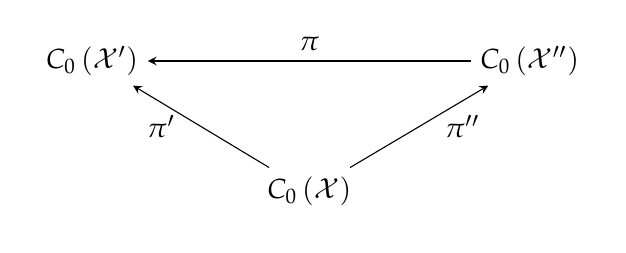
\begin{tikzpicture}
		\matrix (m) [matrix of math nodes,row sep=3em,column sep=4em,minimum width=2em]
		{
		C_0\left(\sX' \right)  & & C_0\left(\sX'' \right) \\ 
			& C_0\left(\sX \right)  & \\};
		\path[-stealth]
		(m-1-3) edge node [above] {$\pi$} (m-1-1)
		(m-2-2) edge node [left]  {$\pi'~~$} (m-1-1)
		(m-2-2) edge node [right] {$~~\pi''$} (m-1-3);
		\end{tikzpicture}
		\\ 	
	\end{itemize}
Following conditions hold:
\begin{enumerate}
	\item [(i)] 	If the category $\mathfrak{FinCov}$-$\sX$ is given by the Definition \ref{top_fin_cov_defn} then there is the natural equivalence of the categories $C_0:\mathfrak{FinCov}$-$\sX \cong \mathfrak{FinCov}$-$C_0\left(\sX \right)$.
	\item[(ii)] Any unordered pair of *-homomorphisms $\left( \pi',\pi''\right) $ from the above diagram is {compliant} (cf. Definition \ref{compliant_covering_defn}).
\end{enumerate}

\end{lem}
\begin{proof}
	(i) From the Theorem \ref{comm_fin_thm} it follows that there is a one-to-one correspondence between objects of $\mathfrak{FinCov}$-$\sX$ and objects of  $\mathfrak{FinCov}$-$C_0\left(\sX \right)$ given by
	$$
	\left(p:\widetilde{\sX} \to \sX \right) \mapsto 	C_0\left( p\right) :   C_0\left( \sX\right)    \hookto C_0\left( \widetilde{\sX}\right)
	$$
	where $C_0\left(p\right)$ is given by the Definition \ref{top_c_funct_defn}. If $p':\widetilde{\sX}' \to \sX$ and $p'':\widetilde{\sX}'' \to \sX$ are objects of $\mathfrak{FinCov}$-$\sX$ and $p: \widetilde{\sX}' \to \widetilde{\sX}''$ is a morphism of $\mathfrak{FinCov}$-$\sX$ then from the Corollary \ref{top_covp_cat_cor} it turns out that $p$ is a transitive finite-fold covering. From the equation \eqref{top_c0_p_eqn} it follows that $p$ corresponds to the injective *-homomorphism
	\be\label{top_c_funct_lem_eqn}
	C_0\left(p \right):  C_0\left( \widetilde{\sX}''\right)    \to C_0\left( \widetilde{\sX}'\right).
	\ee
	So one has a functor from  $\mathfrak{FinCov}$-$\sX$ to  $\mathfrak{FinCov}$-$C_0\left( \sX\right)$. Let us define the inverse  functor. From the Theorem \ref{comm_fin_thm} it follows that any object $\pi: C_0\left( \sX\right) \hookto C_0\left( \widetilde{\sX}\right)$ of $\mathfrak{FinCov}$-$C_0\left( \sX\right) $ corresponds to a transitive finite-fold covering $p: \widetilde{\sX} \to \sX$ such that $\pi = C_0\left(p \right)$. If $C\left(p' \right): C_0\left( {\sX}\right)\to  C_0\left( \widetilde{\sX}'\right) $ and $C\left(p'' \right): C_0\left( {\sX}\right)\to C_0\left( \widetilde{\sX}''\right)$ are objects of $\mathfrak{FinCov}$-$C_0\left( \sX\right)$  and $\pi: C_0\left( \widetilde{\sX}''\right)    \to C_0\left( \widetilde{\sX}'\right)$ is a *-homomorphism such that $ C_0\left(p'\right) = \pi \circ C_0\left(p''\right)$ then from the Lemma \ref{comm_comply_lem} it turns out that there is a finite-fold  transitive covering $p: \widetilde{\sX}' \to \widetilde{\sX}''$ such than  $\pi= C_0\left( p\right) $ and $p'= p \circ p''$. So one has the inverse functor from   $\mathfrak{FinCov}$-$C_0\left( \sX\right)$ to $\mathfrak{FinCov}$-$\sX$.\\
	(ii)	The conditions (a)-(d) of the Definition \ref{compliant_covering_defn} directly follow from (a)-(d) of the Lemma \ref{comm_comply_lem}.
	\end{proof}


\subsection{Induced representation}\label{comm_induced_finite_sec}
 \paragraph*{} 
Let us consider a compact  Riemannian manifold $M$ with a  spin bundle $\sS$ (cf. \ref{spin_mani_sec}). Denote by $\mu$  the Riemannian measure (cf.  \cite{do_carmo:rg}) on $M$ which corresponds to the given by  the Equation \eqref{top_vol_eqn} volume element. The bundle $S$ is Hermitian (cf. Definition \ref{top_herm_bundle_defn}) so there is a Hilbert space $L^2\left( M, S, \mu\right)$ (or  $L^2\left( M, S\right)$ in a simplified notation) (cf. \ref{top_herm_bundle_empt}) with the given by \eqref{top_bundle_herm_scalar_eqn} scalar product, i.e.
\be\label{comm_bundle_herm_scalar_eqn}
	\left( \xi, \eta\right)_{L^2\left(M, S\right)}\stackrel{\text{def}}{=} \int_{M}\left( \xi_x, \eta_x\right)_xd\mu.
\ee
Moreover from 	\eqref{comm_bundle_repr_eqn} it follows that there is the natural representation
\be\label{comm_m_bundle_repr_eqn}
C\left(M\right) \to B\left( L^2\left(  M, S\right)\right). 
\ee
From \ref{top_herm_bundle_empt} it follows that $L^2\left( M, S, \mu\right)$ is the Hilbert norm completion of $\Ga\left(M, \sS\right)$. On the other hand from the Lemma \ref{top_bundle_cs_lem}  it follows that $\Ga\left(M, \sS\right)$ is {continuity structure for} $\sX$ {and the} $\left\{\SS_x\right\}_{x \in \sX}$ (cf. Definition \ref{op_fields_defn}), such that
$$
\Ga\left(M, \sS\right) \cong C\left(M, \left\{\SS_x\right\},  \Ga\left(M, \sS\right)\right). 
$$
If $p: \widetilde{M} \to M$ is a finite-fold  transitive covering then from the Lemma \ref{top_tensor_comact_lem} it follows that there is the natural isomorphism
\be\label{top_lift_g_eqn}
	\phi: C\left(\widetilde \sX\right)\otimes_{C\left(M\right)} C\left(M,\left\{\SS_x\right\},  \Ga\left(M, \sS\right)\right) \xrightarrow{\approx}\lift_p\left[C\left(M, \left\{\SS_x\right\},  \Ga\left(M, \sS\right)\right)\right]
\ee
of $C\left(\widetilde{M} \right)$-modules. From the Lemma \ref{top_lift_bundle_lem} it follows that $\lift_p\left[C\left(M, \left\{\SS_x\right\},  \Ga\left(M, \sS\right)\right)\right]\cong \Ga\left(\widetilde{M}, \widetilde{\SS} \right)$ where $\widetilde{\SS}$ is the {inverse image} of $\SS$ by $p$ (cf. Definition \ref{vb_inv_img_funct_defn}). Hence the equation \eqref{top_lift_g_eqn} can be rewritten by the following way
\be\label{top_lift_gs_eqn}
\phi: C\left(\widetilde M\right)\otimes_{C\left(M\right)} \Ga\left(M, \sS\right) \xrightarrow{\approx} \Ga\left(\widetilde{M}, \widetilde{\SS} \right)
\ee
\begin{lemma}\label{top_hilb_homo_lem}
Following conditions hold:
	\begin{itemize}
		\item [(i)] The map \eqref{top_lift_gs_eqn} can be extended up to the following homomorphism 
		$$
		C\left(\widetilde M\right)\otimes_{C\left(M\right)} L^2\left(M, \sS\right) \xrightarrow{\approx} L^2\left(\widetilde{M}, \widetilde{\SS} \right)
		$$
		of left $C\left(\widetilde M\right)$-modules.
		\item[(ii)] The image of $C\left(\widetilde M\right)\otimes_{C\left(M\right)} L^2\left(M, \sS\right)$ is dense in $L^2\left(\widetilde{M}, \widetilde{\SS} \right)$.
	\end{itemize}
\end{lemma}
\begin{proof}(i)
Let $\sum_{j = 1}^n \widetilde a_j \otimes \xi_j\in 	C\left(\widetilde M\right)\otimes_{C\left(M\right)} L^2\left(M, \sS\right)$ be any element. From  \ref{top_herm_bundle_empt} $L^2\left( M, S, \mu\right)$ is the Hilbert norm completion of $\Ga\left(M, \sS\right)$. Hence for any $j =1,..., n$ there is a net $\left\{\xi_{j\a}\right\}\subset \Ga\left(M, \sS\right)$ such that $\xi_j = \lim_\a \xi_{j\a}$ where we mean the convergence with respect to the Hilbert norm $\left\| \cdot\right\|_{L^2\left(M, \sS\right)}$. If $C = \max_{j = 1,...,n}\left\|\widetilde a_j\right\|$ then there is $\a_0$ such that
$$
\a \ge \a_0 \quad \Rightarrow \left\| \xi_j - \xi_{j\a}\right\|_{L^2\left(M, \sS\right)} < \frac{\eps}{nC},
$$
so one has
$$
\a \ge \a_0 \quad \Rightarrow \left\| \sum_{j = 1}^n \widetilde a_j \otimes \xi_{j\a_0} - \sum_{j = 1}^n \widetilde a_j \otimes \xi_{j\a}\right\|_{L^2\left(\widetilde M, \widetilde\sS\right)} < \eps.
$$
The above equation it follows that the net $\left\{\sum_{j = 1}^n \widetilde a_j \otimes \xi_{j\a}\right\}_\a$ satisfies to the Cauchy condition, so it is convergent with respect to the topology of $L^2\left(\widetilde M, \widetilde\sS\right)$.\\
(ii) From the Lemma \ref{top_tensor_comact_lem} it follows that the image of $C\left(\widetilde M\right)\otimes_{C\left(M\right)} L^2\left(M, \sS\right)$ in $L^2\left(\widetilde M, \widetilde\sS\right)$ contains $\Ga\left(\widetilde{M}, \widetilde{\SS} \right)$, however $\Ga\left(\widetilde{M}, \widetilde{\SS} \right)$ is dense in $L^2\left(\widetilde{M}, \widetilde{\SS} \right)$. It follows that  $\phi\left(  C\left(\widetilde M\right)\otimes_{C\left(M\right)} L^2\left(M, \sS\right)\right)$ is dense in $L^2\left(\widetilde{M}, \widetilde{\SS} \right)$. 
\end{proof}
\begin{remark}
	Indeed the image of $C\left(\widetilde M\right)\otimes_{C\left(M\right)} L^2\left(M, \sS\right)$ coincides with $L^2\left(\widetilde{M}, \widetilde{\SS} \right)$. However this fact is not used here.
\end{remark}
Let both $\mu$ and $\widetilde{\mu}$ be Riemannian measures (cf.  \cite{do_carmo:rg}) on both $M$ and $\widetilde{M}$ respectively which correspond to both the volume element (cf. \eqref{top_vol_eqn}) and its $p$-lift (cf. \eqref{top_vol_lift_eqn}).
If $\widetilde{a} \otimes \xi, \widetilde{b} \otimes \eta \in C\left(\widetilde{M} \right) \otimes_{C\left(M \right) } \Ga\left( M, S\right) \subset L^2\left(\widetilde{M},\widetilde{S} \right)$  then  the given by the Equation \eqref{induced_prod_equ} scalar product $\left(\cdot, \cdot \right)_{\text{ind}}$ on  $ \Ga\left( M, S\right) \otimes L^2\left({M},{S}, \mu\right)$ satisfies to the following equation
\begin{equation}\label{comm_ind_l2_eqn}
\begin{split}
\left( \widetilde{a} \otimes \xi ,    \widetilde{b} \otimes \eta\right)_{\text{ind}}= \left(\xi, \left\langle \widetilde{a}, \widetilde{b}\right\rangle_{C\left(\widetilde{M} \right) } \eta \right)_{L^2\left({M},{S} \right)}=\\=\sum_{\widetilde{\a}\in \widetilde{\mathscr A}}\left(\xi, \left\langle \widetilde{a}_{\widetilde{\a}}\widetilde{a}, \widetilde{b}\right\rangle_{C\left(\widetilde{M} \right) } \eta \right)_{L^2\left({M},{S} \right)}
= \sum_{\widetilde{\a}\in \widetilde{\mathscr A}}\left(\xi, \mathfrak{desc}\left( \widetilde{a}_{\widetilde{\a}} \widetilde{a}^* \widetilde{b}\right)  \eta \right)_{L^2\left({M},{S} \right)}=
\\
=
\sum_{\widetilde{\a}\in \widetilde{\mathscr A}}~\int_M \left(\xi_x, \mathfrak{desc}\left( \widetilde{a}_{\widetilde{\a}} \widetilde{a}^* \widetilde{b}\right)  \eta_x \right)_x d\mu=
\\
=
\sum_{\widetilde{\a}\in \widetilde{\mathscr A}}~\int_M \left(\mathfrak{desc}\left( \widetilde{e}_{\widetilde{\a}} \widetilde{a}\right)\xi_x, \mathfrak{desc}\left( \widetilde{e}_{\widetilde{\a}}  \widetilde{b}\right)  \eta_x \right)_x d\mu=
\\
=\sum_{\widetilde{\a}\in \widetilde{\mathscr A}}~ \int_{\widetilde{M}}\left(\widetilde{a} \lift_{\widetilde{\sU}_{\widetilde{\a}}}\left({e}_{\widetilde{\a}}\xi \right)_{\widetilde{x}},  \widetilde{b} ~\lift_{\widetilde{\sU}_{\widetilde{\a}}}\left({e}_{\widetilde{\a}}\eta \right)_{\widetilde{x}}\right)_{\widetilde{x}}d \widetilde{   \mu} =
\\
=\sum_{\widetilde{\a}\in \widetilde{\mathscr A}}~ \int_{\widetilde{M}}\widetilde{a}_{\widetilde{\a}}\left(\widetilde{a} \lift_{\widetilde{\sU}_{\widetilde{\a}}}\left(\xi \right)_{\widetilde{x}},  \widetilde{b} ~\lift_{\widetilde{\sU}_{\widetilde{\a}}}\left(\eta \right)_{\widetilde{x}}\right)_{\widetilde{x}}d \widetilde{   \mu} =
\\
= \int_{\widetilde{M}}\left( \widetilde{a} \lift_p\left(\xi \right)_{\widetilde{x}},  \widetilde{b} ~\lift_p\left(\eta \right)_{\widetilde{x}}\right)_{\widetilde{x}}d \widetilde{   \mu}
= \left( \widetilde{a}~ \lift_p\left(\xi \right),  \widetilde{b} ~\lift_p\left(\eta \right)\right)_{L^2\left(\widetilde{M},\widetilde{S} \right)} =\\
=  \left(\phi\left(  \widetilde{a}\otimes\xi\right) ,  \phi \left( \widetilde{b}\otimes\eta\right)\right)_{L^2\left(\widetilde{M},\widetilde{S} \right)}
\end{split} 
\end{equation}
where $\phi$ is given by \eqref{top_tensor_comact_iso_eqn} and both finite families $\left\{\widetilde{a}_{\widetilde{\a}}\right\}_{\widetilde{\a}\in \widetilde{\mathscr A}},~\left\{\widetilde{e}_{\widetilde{\a}}\right\}_{\widetilde{\a}\in \widetilde{\mathscr A}}\subset C\left(\widetilde M \right) $ are explained in the Remark \ref{comm_unity_rem}.
The equation \eqref{comm_ind_l2_eqn} means that $\left(\cdot, \cdot \right)_{\text{ind}}= \left(\cdot, \cdot \right)_{L^2\left(\widetilde{M},\widetilde{S} \right)}$, and taking into account the dense inclusion $C\left(\widetilde{M} \right) \otimes_{C\left(M \right) } \Ga\left( M, S\right) \subset L^2\left(\widetilde{M},\widetilde{S} \right)$ with respect to the Hilbert norm of $L^2\left(\widetilde{M},\widetilde{S}\right) $
one concludes that the space of induced representation coincides with $L^2\left(\widetilde{M},\widetilde{S}\right)$. It means that induced representation $C\left(\widetilde{M}\right) \times L^2\left(\widetilde{M},\widetilde{S} \right) \to L^2\left(\widetilde{M},\widetilde{S} \right)$ is given by \eqref{comm_bundle_repr_eqn}. So one has the following lemma.
\begin{lemma}\label{comm_ind_lem}
If the representation  $\widetilde{\rho}: C\left(\widetilde{M}\right) \to  B\left( \widetilde{   \H}\right)  $ is induced by the pair $$\left(C\left(M \right)\to B\left(  L^2\left(M,S \right)\right) ,\left(C\left(M \right) , C\left( \widetilde{M}\right) , G\left( \left.\widetilde{M}~\right|M\right) \right)  \right)$$ (cf. Definition \ref{induced_repr_defn}) then following conditions holds
\begin{enumerate}
	\item[(a)] There is the homomorphism of Hilbert spaces $\widetilde{   \H}\cong L^2\left(\widetilde{M},\widetilde{S} \right)$,
	\item[(b)] The representation $\widetilde{\rho}$ is given by the natural action of $C\left(\widetilde{M}\right)$ on $ L^2\left(\widetilde{M},\widetilde{S} \right)$ (cf.   \eqref{comm_bundle_repr_eqn}).
\end{enumerate}
\end{lemma}
\begin{proof}
	(a) Follows from \eqref{comm_ind_l2_eqn}.\\
	(b) From the Lemma \ref{top_hilb_homo_lem}  it follows that the map 		$	C\left(\widetilde M\right)\otimes_{C\left(M\right)} L^2\left(M, \sS\right) \xrightarrow{\approx} L^2\left(\widetilde{M}, \widetilde{\SS} \right)$ is the homomorphism of $C\left(\widetilde M\right)$ modules, so the given by \eqref{comm_bundle_repr_eqn} $C\left(\widetilde M\right)$-action coincides with the $C\left(\widetilde M\right)$-action  the given by \eqref{ind_act_form_eqn}.
	\end{proof}

\begin{remark}\label{comm_ind_rem}
	If the spectral triple $\left( \Coo\left(\widetilde M \right), L^2\left(\widetilde M, \widetilde S, \widetilde\mu\right), \widetilde \Dslash \right)$ is the {geometrical} $p$-{lift} of the spectral triple $\left( \Coo\left( M \right), L^2\left( M,  S, \mu\right),  \Dslash \right)$ (cf. Definition \ref{top_geom_lift_defn}), then clearly the corresponding to $\left( \Coo\left( M \right), L^2\left( M,  S, \mu\right),  \Dslash \right)$ representation of $C\left(M \right)$ equals to the given by the Lemma \ref{comm_ind_lem} representation .
\end{remark}

\subsection{Coverings of spectral triples}\label{comm_d_sec}
Consider the situation of the Section \ref{comm_induced_finite_sec}. Suppose that 
\be\label{top_ta_eqn}
		\sum_{g \in G\left(\left.\widetilde{M}~\right|M\right),~ \a \in \mathscr A  } g\widetilde{a}_\a = 1_{C\left(\widetilde{M} \right) }
\ee
is the compliant with  the covering $p:\widetilde{M}\to{M}$ partition of unity (cf. Definition \ref{comm_comply_defn}). The space $M$ is compact, hence one can suppose that the set $\mathscr A $ is finite.  If we denote by $\widetilde{ \mathscr A}\bydef   G\left(\left.\widetilde{M}~\right|M\right)\times \mathscr A$ then the above partition of unity is the following finite sum
\bean
\sum_{ \widetilde\a \in \widetilde{ \mathscr A} } \widetilde{a}_{\widetilde\a} = 1_{C\left(\widetilde{M} \right) }.
\eean
From the Proposition \ref{smooth_part_unity_prop} one can assume that $\widetilde{a}_{\widetilde\a}\in \Coo\left( \widetilde{M}\right)$ and
\be\label{top_te_eqn}
\begin{split}
	\widetilde{e}_{\widetilde\a}\bydef \sqrt{\widetilde{a}_{\widetilde\a}}\in \Coo\left( \widetilde{M}\right),\\
	\sum_{ \widetilde\a \in \widetilde{ \mathscr A} } \widetilde{e}^2_{\widetilde\a} =\sum_{ \widetilde\a \in \widetilde{ \mathscr A} } \widetilde{e}_{\widetilde\a} \desc_p\left(\widetilde{e}_{\widetilde\a} \right)= 1_{C\left(\widetilde{M} \right) }.
\end{split}
\ee 
\begin{lemma}\label{top_smooth_matr_lem}
Following conditions hold:
\begin{itemize}
	\item [(i)] The finite family $\left\{	\widetilde{e}_{\widetilde\a}\right\}_{\widetilde\a \in \widetilde{ \mathscr A}}$  satisfies to the Lemma \ref{smooth_matr_lem}.
		\item[(ii)] 
	\be\label{top_smooth_lcond_eqn}
C\left(\widetilde M \right)  \cap \mathbb{M}_{\left|\widetilde{\mathscr A}~ \right|}\left(\Coo\left( M\right)\right) = \Coo\left(\widetilde M \right). 
	\ee
	\item[(iii)] The  given by the Corollary \ref{comm_comm_cor} unital noncommutative finite-fold covering \\$\left(C\left(M \right) , C\left( \widetilde{M}\right) , G\left( \left.\widetilde{M}~\right|M\right) \right)$  is smoothly invariant (cf. Definition \ref{smooth_defn}).
\end{itemize}
\end{lemma}
\begin{proof}
	(i)
For any $\widetilde{a} \in C\left( \widetilde{M}\right)$ from \eqref{top_te_eqn} it follows that
$$
\widetilde{a} = \sum_{ \widetilde{\a}\in {\widetilde{\mathscr A}}} \widetilde{e}_{\widetilde\a} \left\langle \widetilde{e}_{\widetilde\a}, \widetilde{a}\right\rangle_{\widetilde{A}} \in \sum_{ \widetilde{\a}\in {\widetilde{\mathscr A}}} \widetilde{e}_{\widetilde\a}C\left(M\right),
$$
i.e. the right $C\left(M \right)$-module $C\left( \widetilde{M}\right)$ is generated by the finite set $\left\{\widetilde{e}_{\widetilde\a}\right\}$; that is
$$
C\left( \widetilde{M}\right) = \sum_{ \widetilde{\a}\in \widetilde{\mathscr A}}\widetilde{e}_{\widetilde\a}C\left(M\right).
$$
Let us prove that $\left\{\widetilde{e}_{\widetilde\a}\right\}$ satisfies to conditions (a) and (b) of the Lemma \ref{smooth_matr_lem}.
\begin{enumerate}
	\item [(a)] One has 
	$$
	\left\langle \widetilde{e}_{\widetilde{\a'}}, \widetilde{e}_{\widetilde{\a''}}\right\rangle_{C\left(\widetilde{M} \right) }= \sum_{g \in  G\left( \left.\widetilde{M}~\right|M\right)} g\left(\widetilde{e}^*_{\widetilde{\a'}}, \widetilde{e}_{\widetilde{\a''}} \right), 
	$$
	so from $\widetilde{e}_{\widetilde{\a'}}, \widetilde{e}_{\widetilde{\a''}}\in \Coo\left( \widetilde M\right)$ it turns out that 	$\left\langle \widetilde{e}_{\widetilde{\a'}}, \widetilde{e}_{\widetilde{\a''}}\right\rangle_{C\left(\widetilde{M} \right) }\in \Coo\left(M \right)$.
	\item[(b)]  	The given by the  Equation \eqref{top_ta_eqn} set $\left\{ g\widetilde{a}_\a\right\}_{g \in G\left(\left.\widetilde{M}~\right|M\right),~ \a \in \mathscr A  }$  is $G\left(\left.\widetilde{M}~\right|M\right)$-invariant, hence from $	\widetilde{e}_{\widetilde\a}\bydef \sqrt{\widetilde{a}_{\widetilde\a}}$ it turns out that the family $\left\{\widetilde{e}_{\widetilde\a}\right\}$ is also $G\left(\left.\widetilde{M}~\right|M\right)$-invariant.
\end{enumerate}
(ii) From (i) the  Lemma \ref{smooth_matr_lem} it follows that
\be\label{top_smooth_cond_eqn}
\begin{split}
	C\left(\widetilde M \right)  \cap \mathbb{M}_n\left(\Coo\left( M\right)  \right)= \\
	=\left\{ 	\widetilde{a}\in 	C\left(M \right) ~|~  \left\langle \widetilde{e}_{\widetilde{\a'}}, \widetilde{a}\widetilde{e}_{\widetilde{\a''}}\right\rangle_{C\left(\widetilde M \right) } \in \Coo\left(M \right) ; ~\forall \widetilde{\a'}, \widetilde{\a''} \in \widetilde{\mathscr A}\right\} 
\end{split}
\ee
From $\widetilde{e}_{\widetilde{\a'}}, \widetilde{e}_{\widetilde{\a''}}\in \Coo\left(\widetilde M \right)$ it turns out that any $\widetilde a\in \Coo\left(\widetilde M \right)$ satisfies to the right part of \eqref{top_smooth_cond_eqn}. If $\widetilde{a} \in C\left( \widetilde{M}\right) \setminus \Coo\left(\widetilde{M} \right)$ then there is point $\widetilde x \in \widetilde{M}$ such that $\widetilde{a}$ is not smooth at $\widetilde x $. There is $\widetilde{\a} \in \widetilde{\mathscr A}$ such that $\widetilde{e}_{\widetilde{\a}} \left( \widetilde x \right)  \neq 0$, so $\widetilde{e}^2_{\widetilde{\a}}\widetilde{a}$ is not smooth at $\widetilde x $. On the other hand one has $\left\langle \widetilde{e}_{\widetilde{\a}}, \widetilde{a}\widetilde{e}_{\widetilde{\a}}\right\rangle_{C\left(\widetilde M \right) }= \desc_p\left(\widetilde{a}\widetilde{e}^2_{\widetilde{\a}} \right)$ is not smooth at $p\left( \widetilde x \right)$ so  $\widetilde{\a}$ does not match to right part of \eqref{top_smooth_cond_eqn}, i.e. $\widetilde{a}\notin C\left(\widetilde M \right)  \cap \mathbb{M}_n\left(\Coo\left( M\right)\right)$. In result one has 
\be\label{top_smooth_l_eqn}
\begin{split}
	C\left(\widetilde M \right)  \cap \mathbb{M}_n\left(\Coo\left( M\right)  \right)= \Coo\left(\widetilde{M} \right).
\end{split}
\ee
(iii) From (ii) the  Lemma \ref{smooth_matr_lem}. 
\end{proof}
For any $\widetilde{a} \in \Coo\left(\widetilde{M} \right)$ following condition holds
\be\label{top_ph_ps_eqn}
\widetilde{a} = \sum_{\widetilde{\a}\in \widetilde{\mathscr A}} \widetilde{\ga}_{\widetilde{\a}}= \sum_{\widetilde{\a}\in \widetilde{\mathscr A}} \widetilde{\phi}_{\widetilde{\a}}\widetilde{\psi}_{\widetilde{\a}}; \text{ where } \widetilde{\phi}_{\widetilde{\a}}= \widetilde{e}_{\widetilde{\a}},~ \widetilde{\psi}_{\widetilde{\a}}= \widetilde{e}_{\widetilde{\a}}\widetilde{a},~ \widetilde{\ga}_{\widetilde{\a}}=\widetilde{a}_{\widetilde{\a}}\widetilde{e}^2_{\widetilde{\a}}.
\ee
Denote by $\Om^1_{\slashed D}$  the {module of differential forms associated} with the given by  \eqref{comm_sp_tr_eqn} spectral triple  $\left(\Coo\left({M} \right), L^2\left(M,S \right), \slashed D\right)$ (cf. Definition \ref{ass_cycle_defn}). Denote by 
\be\label{top_descs_eqn}
{\phi}_{\widetilde{\a}} \bydef \mathfrak{desc} \left(\widetilde{\phi}_{\widetilde{\a}} \right),\quad {\psi}_{\widetilde{\a}} \bydef \mathfrak{desc} \left(\widetilde{\psi}_{\widetilde{\a}} \right), \quad {\ga}_{\widetilde{\a}} \bydef \mathfrak{desc} \left(\widetilde{\ga}_{\widetilde{\a}} \right)\in \Coo\left({M} \right)
\ee
 Let us define a $\C$-linear map
\be\label{top_nabla_eqn}
\begin{split}
\widetilde{\slashed{\nabla}}: \Coo\left(\widetilde{M} \right) \to \Coo\left(\widetilde{M} \right) \otimes_{\Coo\left({M} \right)}\Om^1_{\slashed D},\\
\widetilde{a} \mapsto \sum_{\widetilde{\a}\in \widetilde{\mathscr A}}\left(  \widetilde{\phi}_{\widetilde{\a}} \otimes \left[\slashed D, {\psi}_{\widetilde{\a}}  \right] +\widetilde{\psi}_{\widetilde{\a}} \otimes \left[\slashed D, {\phi}_{\widetilde{\a}}   \right] \right).
\end{split}
\ee
For any $a \in \Coo\left({M} \right)$ from $\left[\slashed D, {\psi}_{\widetilde{\a}} a  \right] = {\psi}_{\widetilde{\a}} \left[\slashed D, a  \right] + \left[\slashed D, {\psi}_{\widetilde{\a}}   \right]a$, $\widetilde{\phi}_{\widetilde{\a}} \otimes {\psi}_{\widetilde{\a}}$ = $\widetilde{\phi}_{\widetilde{\a}}  \widetilde{\psi}_{\widetilde{\a}}\otimes 1_{\Coo\left( M\right) }$ and \eqref{comm_matr_x_eqn} it follows that
 \bean
 \widetilde{\slashed{\nabla}}\left(\widetilde{a}a \right)=  \sum_{\widetilde{\a}\in \widetilde{\mathscr A}}\left(  \widetilde{\phi}_{\widetilde{\a}} \otimes \left[\slashed D, {\psi}_{\widetilde{\a}} a  \right] +\widetilde{\psi}_{\widetilde{\a}}a \otimes \left[\slashed D, {\phi}_{\widetilde{\a}}   \right] \right) =
 \\
 = \sum_{\widetilde{\a}\in \widetilde{\mathscr A}}\left(  \widetilde{\phi}_{\widetilde{\a}} \otimes \left[\slashed D, {\psi}_{\widetilde{\a}}  \right]a+\widetilde{\phi}_{\widetilde{\a}} \otimes {\psi}_{\widetilde{\a}}\left[\slashed D,  a  \right] +\widetilde{\psi}_{\widetilde{\a}} \otimes a \left[\slashed D, {\phi}_{\widetilde{\a}}   \right]\right) =
 \\
 = \sum_{\widetilde{\a}\in \widetilde{\mathscr A}}\left(  \widetilde{\phi}_{\widetilde{\a}} \otimes \left[\slashed D, {\psi}_{\widetilde{\a}}  \right]a+\widetilde{\phi}_{\widetilde{\a}} \widetilde{\psi}_{\widetilde{\a}}\otimes \left[\slashed D,  a  \right] +\widetilde{\psi}_{\widetilde{\a}} \otimes  \left[\slashed D, {\phi}_{\widetilde{\a}}   \right]a\right) =
 \\
 = \sum_{\widetilde{\a}\in \widetilde{\mathscr A}}\left(  \widetilde{\phi}_{\widetilde{\a}} \otimes \left[\slashed D, {\psi}_{\widetilde{\a}}   \right] +\widetilde{\psi}_{\widetilde{\a}} \otimes \left[\slashed D, {\phi}_{\widetilde{\a}}  \right] \right) a+
 \sum_{\widetilde{\a}\in \widetilde{\mathscr A}}\widetilde{\phi}_{\widetilde{\a}}\widetilde{\psi}_{\widetilde{\a}}\otimes\left[ \slashed D,a\right]=
 \widetilde{\slashed{\nabla}}\left( \widetilde{a}\right) a + \widetilde{a}\otimes  \left[ \slashed D,a\right]. 
 \eean
The comparison of the above equation and \eqref{conn_triple_eqn} states that $\widetilde{\slashed{\nabla}}$ is a connection. If $g \in  G\left( \left.\widetilde{M}~\right|M\right)$ then from $\mathfrak{desc}\left(g\widetilde{\phi}_{\widetilde{\a}}\right) = {\phi}_{\widetilde{\a}} $ and $\mathfrak{desc}\left(g\widetilde{\psi}_{\widetilde{\a}}\right) = {\psi}_{\widetilde{\a}} $ it follows that
\bean
\widetilde{\slashed{\nabla}}\left(g\widetilde{a} \right)=  \widetilde{\slashed{\nabla}}\left(\sum_{\widetilde{\a}\in \widetilde{\mathscr A}} \left( g\widetilde{\phi}_{\widetilde{\a}}\right) \left( g\widetilde{\psi}_{\widetilde{\a}}\right)\right)=\\=\sum_{\widetilde{\a}\in \widetilde{\mathscr A}}\left( g \widetilde{\phi}_{\widetilde{\a}} \otimes \left[\slashed D, {\psi}_{\widetilde{\a}}   \right] +g\widetilde{\psi}_{\widetilde{\a}} \otimes \left[\slashed D, {\phi}_{\widetilde{\a}}   \right] \right)= g \left( \widetilde{\slashed{\nabla}}\left(\widetilde{a} \right)\right),  
\eean
i.e. $\widetilde{\slashed{\nabla}}$ is  $G\left( \left.\widetilde{M}~\right|M\right)$-{equivariant} (cf. \eqref{equiv_conn_eqn}). 
Similarly to \eqref{top_tensor_comact_iso_eqn} one can define a $\Coo\left(\widetilde M \right)$-module  homomorphism
\be\label{top_phinf_eqn}
\begin{split}
\phi_\infty :\Coo\left(\widetilde M \right)\otimes \Ga^\infty\left(M, \sS \right)  \to \Ga^\infty\left(\widetilde M, \widetilde\sS \right),\\
\sum_{j=1}^n \widetilde a_j \otimes \xi_j\mapsto  \sum_{j=1}^n\widetilde a_j \lift_p\left(\xi_j\right)
\end{split}
\ee
where both   $\Ga^\infty\left(M, \sS \right)$ and $\Ga^\infty\left(\widetilde M, \widetilde\sS \right)$ are  defined by the Equations  \eqref{top_smooth_m_eqn} and \eqref{top_lift_sheaf_eqn} respectively.
\begin{lemma}\label{top_phinf_lem}
The given by the Equation \eqref{top_phinf_eqn} homomorphism is an isomorphism.
\end{lemma}
\begin{proof}
The proof of the Lemma \ref{top_tensor_comact_lem} uses the partition of unity. However from the Proposition \ref{smooth_part_unity_prop} it turns out that there is a smooth partition of unity. Using it one can proof this lemma as well as the Lemma \ref{top_tensor_comact_lem} has been proved.
\end{proof}

Now we have  the  $G\left( \left.\widetilde{M}~\right|M\right)$-{equivariant} connection $\widetilde{\slashed{\nabla}}$, so on can find the specialization of explained in  \ref{triple_conn_lift_empt} construction of the operator
$\widetilde{D} : \widetilde{\A} \otimes_{\A} \H^\infty \to \widetilde{\A} \otimes_{\A} \H^\infty$. The following table reflects the mapping between general theory and the commutative specialization\\ \\
 \begin{tabular}{|c|c|c|}
	\hline
	&General theory & Commutative specialization\\ 
	\hline
	&	&\\
	Hilbert spaces & $\H$  and $\widetilde\H$ &  $L^2\left(M, \sS \right)$ and $L^2\left(\widetilde M, \widetilde \sS \right)$\\ & & \\
Pre-$C^*$-algebras	& $\A$ and $\widetilde\A$ & $\Coo\left(M \right)$ and $\Coo\left(\widetilde M \right)$   \\  & & \\
Dirac operators & $D$ & $\Dslash$  \\
 & $\widetilde{D}$ & ?\\  & & \\
 &$\H^\infty\bydef \bigcap_{n =1}^\infty \Dom D^n\subset \H$ & $\Ga^\infty\left(M, \sS \right)= \bigcap_{n =1}^\infty \Dom \Dslash^n$ \\& & \\
	\hline
\end{tabular}
\\
\\
\\
If $\slashed\nabla \widetilde{a}= \sum_{j = 1}^m\widetilde{a}_j \otimes \om_j\in \Coo\left(\widetilde M \right)\otimes_{\Coo\left( M \right)}\Om^1_{\Dslash}$ then for all $\xi \in \Ga^\infty\left(M, \sS \right)$ denote by
$$
\widetilde{a}_\xi = \phi_\infty\left(\sum_{j = 1}^m\widetilde{a}_j \otimes \om_j\left( \xi\right)  \right)= \sum_{j=1}^m\widetilde a_j \lift_p\left(\om_j\left( \xi\right)\right)\in \Ga^\infty\left(\widetilde M, \widetilde\sS \right)
$$
where $\phi_\infty$ is given by the Equation \eqref{top_phinf_eqn}, and taking into account the Equation \eqref{top_nabla_eqn} one has
$$
\widetilde{a}_\xi = \sum_{\widetilde{\a}\in \widetilde{\mathscr A}}\left(  \widetilde{\phi}_{\widetilde{\a}} \lift_p\left(  \left[\slashed D, {\psi}_{\widetilde{\a}}  \right]\xi \right)  +\widetilde{\psi}_{\widetilde{\a}} \lift_p\left( \left[\slashed D, {\phi}_{\widetilde{\a}}   \right]\xi\right)  \right).
$$
The partition of unity \eqref{top_ta_eqn} compliant with  the covering $p:\widetilde{M}\to{M}$, so for any $\widetilde{\a}\in \widetilde{\mathscr A}$ there is an open subset $\widetilde{\sU}_{\widetilde \a}\subset \widetilde M$ such that 
\begin{itemize}
	\item $\supp \widetilde{a}_{\widetilde \a} \subset \widetilde{\sU}_{\widetilde \a}$.
	\item The restriction $\left.p\right|_{\widetilde{\sU}_{\widetilde \a}}$ is injective. 
\end{itemize}
From \eqref{top_ph_ps_eqn} it follows that $\supp \widetilde{\phi}_{\widetilde \a},\quad \supp \widetilde{\psi}_{\widetilde \a} ,\quad \supp \widetilde{\ga}_{\widetilde \a} \subset \widetilde{\sU}_{\widetilde \a}$. From the Equations \eqref{comm_lift_desc_l_eqn}  and  \eqref{top_descs_eqn} it follows that
$$
\widetilde{\phi}_{\widetilde \a}= \lift^p_{\widetilde{\mathcal U}_{\widetilde \a}}\left(\phi_{\widetilde \a} \right), \quad  \widetilde{\psi}_{\widetilde \a}= \lift^p_{\widetilde{\mathcal U}_{\widetilde \a}}\left(\psi_{\widetilde \a} \right), \quad  \widetilde{\ga}_{\widetilde \a}= \lift^p_{\widetilde{\mathcal U}_{\widetilde \a}}\left(\ga_{\widetilde \a} \right),
$$ hence one has
\bean
\widetilde{a}_\xi = \sum_{\widetilde{\a}\in \widetilde{\mathscr A}}\left(  \lift^p_{\widetilde{\mathcal U}_{\widetilde \a}}\left(\phi_{\widetilde \a} \right) \lift_p\left(  \left[\slashed D, {\psi}_{\widetilde{\a}}  \right]\xi \right)  +\lift^p_{\widetilde{\mathcal U}_{\widetilde \a}}\left(\psi_{\widetilde \a} \right) \lift_p\left( \left[\slashed D, {\phi}_{\widetilde{\a}}   \right]\xi\right)  \right)=
\\
= \sum_{\widetilde{\a}\in \widetilde{\mathscr A}}\left(  \lift^p_{\widetilde{\mathcal U}_{\widetilde \a}}\left(\phi_{\widetilde \a}  \left[\slashed D, {\psi}_{\widetilde{\a}}  \right]\xi \right)  +\lift^p_{\widetilde{\mathcal U}_{\widetilde \a}}\left(\psi_{\widetilde \a}  \left[\slashed D, {\phi}_{\widetilde{\a}}   \right]\xi\right)  \right).
\eean
Otherwise from \eqref{comm_matr_x_eqn} it turns out that ${\psi}_{\widetilde{\a}}  \left[\slashed D, {\phi}_{\widetilde{\a}}   \right] =   \left[\slashed D, {\phi}_{\widetilde{\a}}   \right]{\psi}_{\widetilde{\a}}$, so it follows that
\bean
\widetilde{a}_\xi = 
 \sum_{\widetilde{\a}\in \widetilde{\mathscr A}}\left(  \lift^p_{\widetilde{\mathcal U}_{\widetilde \a}}\left(\phi_{\widetilde \a}  \left[\slashed D, {\psi}_{\widetilde{\a}}  \right]\xi \right)  +\lift^p_{\widetilde{\mathcal U}_{\widetilde \a}}\left(\psi_{\widetilde \a} \left[\slashed D, {\phi}_{\widetilde{\a}}   \right]\xi\right)  \right)=
 \\
 =
 \sum_{\widetilde{\a}\in \widetilde{\mathscr A}}\left(  \lift^p_{\widetilde{\mathcal U}_{\widetilde \a}}\left(\phi_{\widetilde \a}  \left[\slashed D, {\psi}_{\widetilde{\a}}  \right]\xi  +\psi_{\widetilde \a} \left[\slashed D, {\phi}_{\widetilde{\a}}   \right]\xi\right)  \right)=
 \\
=\sum_{\widetilde{\a}\in \widetilde{\mathscr A}}\left(  \lift^p_{\widetilde{\mathcal U}_{\widetilde \a}}\left(  \left[\slashed D, \phi_{\widetilde \a} {\psi}_{\widetilde{\a}}  \right]\xi \right)    \right) = \sum_{\widetilde{\a}\in \widetilde{\mathscr A}}\left(  \lift^p_{\widetilde{\mathcal U}_{\widetilde \a}}\left(  \left[\slashed D, \ga_{\widetilde \a}  \right]\xi \right)    \right) .
\eean
If $ p^{-1}\left(\Dslash \right)\in  \mathscr End\left( \mathscr  C^\infty\left(\widetilde M,  \widetilde\sS \right)\right)$ is the   $p$-{inverse image} of $\Dslash$ (cf. Definition \ref{top_smooth_inv_im_defn}) then taking into account  \eqref{comm_lift_comp_eqn} one has
\bean
\widetilde{a}_\xi 
=\sum_{\widetilde{\a}\in \widetilde{\mathscr A}}
\left[p^{-1}\left(\Dslash \right) , \widetilde{\ga}_{\widetilde{\a}}\right]\lift_p\left(\xi \right) =\left[p^{-1}\left(\Dslash \right) , \sum_{\widetilde{\a}\in \widetilde{\mathscr A}}\widetilde{\ga}_{\widetilde{\a}}\right]\lift_p\left(\xi \right)=
\\
= \left[p^{-1}\left(\Dslash \right) , \widetilde{a}\right] \lift_p\left(\xi \right). 
\eean

If $\widetilde{D}$ is the specialization of the given by \eqref{d_defn_eqn} operator then
\bean
\phi_\infty\left(\widetilde{D}\left(\widetilde{a}\otimes \xi \right)  \right) = \widetilde{a}_\xi + \phi_\infty\left( \widetilde{a} \otimes D\xi\right) = 
\\
= \left[p^{-1}\left(\Dslash \right) , \widetilde{a}\right] \lift_p\left(\xi \right)+ \widetilde{a}\lift_p\left(\Dslash\xi \right)=
\\
= \left[p^{-1}\left(\Dslash \right) , \widetilde{a}\right] \lift_p\left(\xi \right)+ \widetilde{a}p^{-1}\left(\Dslash \right)\lift_p\left(\xi \right)=  p^{-1}\Dslash   \widetilde{a} \lift_p\left(\xi \right)=
\\
= p^{-1}\left(\Dslash \right)\phi_\infty\left( \widetilde{a}\otimes\xi\right),
\eean
or, shortly
\be\label{comm_liftd_comp_eqn} 
\phi_\infty\left(\widetilde{D}\left(\widetilde{a}\otimes \xi \right)  \right) = p^{-1}\Dslash \phi_\infty\left( \widetilde{a}\otimes\xi\right),
\ee
However $\phi_\infty$ is the isomorphism, it can be regarded as the identical map, so the equation \eqref{comm_liftd_comp_eqn} is equivalent to 
\be\label{comm_dxi_eqn}
\widetilde{D}\left(\widetilde{a}\otimes \xi \right)   = p^{-1}\left(\Dslash \right)\left( \widetilde{a}\otimes\xi\right),
\ee in result one has
\be\label{comm_d_eqn}
\widetilde{D} =  p^{-1}{\slashed D}.
\ee
In more detail the above formula has the following meaning
\be\label{top_d_det_eqn}
\begin{split}
\widetilde{\slashed{\nabla}}\left(\widetilde{a} \right)= \sum_{j=1}^m \widetilde{a}_j\otimes  \left[\Dslash, a_j \right]~ \Rightarrow~ \sum_{j=1}^m \widetilde{a}_j\otimes  \left[\Dslash, a_j \right]\xi + \widetilde a \otimes \Dslash\xi =p^{-1}{\slashed D}\left(\widetilde a \otimes \xi \right) 
\end{split}
\ee
where  $p^{-1}\Dslash$ is the   $p$-{inverse image} of $\Dslash$ (cf. Definition \ref{top_smooth_inv_im_defn} and Equation \ref{top_mo_eqn}).
\begin{thm}\label{comm_fin_sp_tr_thm} 
Let 	$\left(C^{\infty}\left( M\right) , L^2\left( M, S\right) ,\slashed D\right)$ be a commutative spectral triple and let $p: \widetilde{M} \to M$ be a transitive finite-fold covering. If   $\left(C\left(M \right) , C\left( \widetilde{M}\right) , G\left( \left.\widetilde{M}~\right|M\right)   \right)$ is an unital noncommutative finite-fold covering given by the Corollary \ref{comm_comm_cor} then  the  {geometrical} $p$-{lift} of $\left(C^{\infty}\left( M\right) , L^2\left( M, S\right) ,\slashed D\right)$ (cf. Definition \ref{top_geom_lift_defn}) coincides with the $\left(C\left(M \right) , C\left( \widetilde{M}\right) , G\left( \left.\widetilde{M}~\right|M\right)   \right)$-lift of $\left(C^{\infty}\left( M\right) , L^2\left( M, S\right) ,\slashed D\right)$ (cf. Definition \ref{triple_conn_lift_defn}). 
\end{thm}
\begin{proof}
From the given by Section \ref{top_cov_sp_tr_sec} construction the  the  {geometrical} $p$-{lift} of $\left(C^{\infty}\left( M\right) , L^2\left( M, S\right) ,\slashed D\right)$ equals to $\left(\Coo\left( \widetilde M\right) , L^2\left(\widetilde M, \widetilde S\right) ,\widetilde \Dslash \right)$ where
 \begin{itemize}
 	\item $\widetilde S$ is the $\widetilde{S} = p^*S$ the inverse image of the spin bundle $S$ (cf. Definition \ref{vb_inv_img_funct_defn}).
 	\item The  given by \eqref{comm_bundle_repr_eqn} natural representation $C\left(\widetilde  M\right)\to B\left( L^2\left(\widetilde M, \widetilde S\right) \right)$ is assumed.
 	\item  Operator $\widetilde \Dslash$ can be regarded as 
 \be
 \begin{split}\label{top_ds_eqn}
 	\widetilde \Dslash = p^{-1} \slashed D \in
\mathscr End \left(\mathscr C^\infty \left(\widetilde M, \left\{\widetilde \sS_{\widetilde x}\right\}, \Ga\left(\widetilde M,\widetilde \sS \right) \right) \right)\left(\widetilde M \right) .
 \end{split}	
\ee
 	 \end{itemize}
 	Denote by $\left(\widetilde \A, \widetilde\H, \widetilde D\right)$ the $\left(C\left(M \right) , C\left( \widetilde{M}\right) , G\left( \left.\widetilde{M}~\right|M\right), C_0\left( p\right)   \right)$-lift of\\ $\left(C^{\infty}\left( M\right) , L^2\left( M, S\right) ,\slashed D\right)$. Consider the given by \eqref{top_te_eqn} finite set $\left\{\widetilde{e}_{\widetilde\a}\right\}_{\widetilde{\a}\in \widetilde{\mathscr A}}$ . 
From (iii)	of the Lemma \ref{top_smooth_matr_lem} it turns that $\left(C\left(M \right) , C\left( \widetilde{M}\right) , G\left( \left.\widetilde{M}~\right|M\right)\right)$ is  smoothly invariant. According to the Definition \ref{triple_conn_lift_defn} and taking into account the Equation \eqref{top_smooth_l_eqn} one has $\widetilde \A = C\left(\widetilde M \right)  \cap \mathbb{M}_n\left(\Coo\left( M\right)\right)  = \Coo\left(\widetilde M \right)$. If $\rho: C\left(M \right)\to L^2\left(M, S \right)$ is the representation of the spectral triple 
$\left(C^{\infty}\left( M\right) , L^2\left( M, S\right) ,\slashed D\right)$ then the representation $\widetilde \rho: C\left(\widetilde M \right)\to B\left(\widetilde \H \right)$ of the spectral triple  $\left(\widetilde \A, \widetilde\H, \widetilde D\right)$ is induced by the pair $\left(\rho,\left(C\left(M \right) , C\left( \widetilde{M}\right), G\left( \left.\widetilde{M}~\right|M\right)\right)  \right)$. From the Remark \ref{comm_ind_rem} it follows that the representation $\widetilde \rho$ is equivalent to the  representation, which corresponds to the spectral triple $\left(C^{\infty}\left( M\right) , L^2\left( M, S\right) ,\slashed D\right)$. From \eqref{comm_d_eqn} it follows that $\widetilde{D} =  p^{-1}{\slashed D}$ and taking into account \eqref{top_ds_eqn} one has $\widetilde{D}= \widetilde{\Dslash}$. It result the  $\left(\widetilde \A, \widetilde\H, \widetilde D\right)$ spectral triple is equivalent to the $\left(\Coo\left( \widetilde M\right) , L^2\left(\widetilde M, \widetilde S\right) ,\widetilde \Dslash \right)$ one.
\end{proof}

\subsection{Unoriented spectral triples}\label{comm_sp_tr} 
\paragraph*{}
Let $M$ be an unoriented  Riemannian manifold, and let $p:\widetilde{M} \to M$ be a two listed regular covering by oriented  Riemannian manifold $\widetilde{M}$ which admits a spin$^c$ structure (cf. Definition \ref{spin_str_defn})  given by a spinor bundle $\widetilde\SS$. From the Corollary \ref{comm_comm_cor} it follows that the triple
$
\left(C\left(M \right), C\left(\widetilde M\right), \Z_2\right) 
$ is an unital finite-fold noncommutative covering (cf. Definition \ref{fin_uni_defn}). If there is a bundle $\SS \to M$ is such that $\widetilde\sS$ is the $p$-inverse image of $\SS$  (cf. Definition \ref{vb_inv_img_funct_defn}) then $\SS$ is  a Hermitian vector bundle (cf. Definition \ref{top_herm_bundle_defn}). It follows that there is a Hilbert space $L^2\left(M, \SS \right)$ and the faithful representation $\rho: C\left(M \right) \to B\left( L^2\left(M, \SS \right)\right)$. Similarly to the Lemma \ref{comm_ind_lem} one can proof that  the given by \eqref{comm_bundle_repr_eqn} representation $\widetilde \rho: C\left(\widetilde{M}\right)\hookto B\left(  L^2\left(\widetilde{M},\widetilde{S} \right)\right) $ is induced by the pair $$\left(C\left(M \right)\to B\left(  L^2\left(M,S \right)\right) ,\left(C\left(M \right) , C\left( \widetilde{M}\right) , G\left( \left.\widetilde{M}~\right|M\right) \right)  \right)$$ (cf. Definition \ref{induced_repr_defn}). The manifold $\widetilde{M}$  admits a spin$^c$ structure, so there is the spectral triple $\left(\Coo\left(\widetilde{M},  \right) , L^2\left(\widetilde{M},\widetilde{\sS} \right), \widetilde\Dslash \right)$. Since $\widetilde{\sS}$ is $\Z_2$-invariant the operator $\widetilde\Dslash$ is also $\Z_2$-invariant there is an unbounded operator
\be\label{ctr_def_5_eqn}
\Dslash \bydef \left. \widetilde\Dslash\right|_{L^2\left(\widetilde{M},\widetilde{\sS} \right)^{\Z_2}}
\ee
where the the induced by the map \eqref{induced_g_act_eqn} action $\Z_2 \times L^2\left(\widetilde{M},\widetilde{\sS} \right) \to L^2\left(\widetilde{M},\widetilde{\sS} \right)$ is implied. On the other hand $L^2\left(\widetilde{M},\widetilde{\sS} \right)^{\Z_2}\cong L^2\left({M},{\sS} \right)$. 
\begin{theorem}\label{com_unori_thm}
The described above triple \be\label{comm_equ}
\left(\Coo\left(M \right), L^2\left(\widetilde{M}, \widetilde{\SS}\right)^{\Z_2}=L^2\left({M}, {\SS}\right), \slashed D  \right).
\ee
a commutative unoriented spectral triple (cf. Definition \ref{unoriented_defn}).
\end{theorem}
\begin{proof}
The following table shows the specialization of  objects 1-5 required by the Definition \ref{unoriented_defn}. 
\\ \\
\begin{tabular}{|c|c|c|}
	\hline
	&Definition \ref{unoriented_defn} & Commutative specialization\\ 
	\hline
	&	&\\
	1 & $\A$   &  $\Coo\left(M \right)$ \\ & & \\
	2	& $\left(A, \widetilde A, \Z_2\right)$ & $\left(C\left(M \right), C\left(\widetilde M\right), \Z_2 \right)$   \\  & & \\
	3 & $\rho: A \to B\left(\H \right)$ & $C\left(M \right)\to B\left( L^2\left({M}, {\SS}\right)\right) $  \\ & & \\
4	& $D$ & $\Dslash$ \\  & & \\
5	& $\left(\widetilde{\A}, \widetilde{\H}, \widetilde{D} \right)$ & $\left(\Coo\left(\widetilde M \right), L^2\left({\widetilde M}, {\widetilde \SS}\right),\widetilde\Dslash\right)$ \\& & \\
	\hline
\end{tabular}
\\
\\
\\
Let us proof conditions (a)-(d) of the Definition \ref{unoriented_defn}. Conditions (a)-(c) follow from the discussion at the beginning of the Section \ref{comm_sp_tr}. Let us prove (d).
 The following evident formula
$$
\Coo\left( M \right) =C\left( M \right) \cap \Coo\left(\widetilde M \right)
$$
is the specialization of the Equation \eqref{main_def_4_eqn}. The Equation \eqref{ctr_def_5_eqn}, is the specialization of \eqref{main_def_5_eqn}. 
\end{proof}

\begin{example}
If $S^3$ is the 3-dimensional sphere then the tangent bundle $TS^3$ is trivial. The follows that the bundle $\C\ell\left( S^3\right)  \to S^3$ (cf. \ref{spin_mani_sec}) is also trivial. So there is the trivial spinor bundle $\widetilde\SS \to S^3$, and the spectral triple $\left(\Coo\left(S^3 \right), L^2\left(S^3, {\widetilde \SS}\right),\widetilde\Dslash\right)$ which satisfies to described in  \cite{hajac:toknotes,varilly:noncom} axioms.
 Otherwise there is two listed regular topological covering $p: S^3\to \R P^3$ where $\R P^3$ is the 3-dimensional real projective space. The spinor bundle $\widetilde\SS$ is trivial, hence there is the trivial bundle $\SS \to R P^3$ such that $\widetilde\SS$ is the $p$-inverse image of $\sS$. From the Theorem \ref{com_unori_thm} it follows that there is the given by
 $$
 \left(\R P^3, L^2\left(\R P^3, { \SS}\right),\Dslash\right)
 $$
 unoriented spectral triple.
\end{example}




\section{Infinite coverings}

\subsection{Inverse limits of coverings in topology}\label{top_inf_to_sec}
%\paragraph*{}
\begin{empt}\label{top_inv_empt}
	Let $\sX$ be a connected, locally connected, locally compact, Hausdorff  topological space. Let $\left\{p_\la: \sX_\la\to\sX\right\}_{\la \in \La}$ be a family of transitive finite-fold coverings which is indexed by a countable set $\La$ such that $\sX_\la$ is connected for all $\la\in\La$. Let us define an order on $\La$ such that 
	\be\label{top_ord_eqn}
	\begin{split}
		\mu \ge \nu  \text{ if and only if there is a surjective coninuous map } p: \sX_\mu \to \sX_\nu \\
		\text{ such that } p_\mu = p_\nu \circ p .
	\end{split}
	\ee
	From the Corollary \ref{top_cov_cat_cor} it follows that the map $p$ is a covering. Suppose that there is the minimal $\la_{\min}\in \La$ such that $\sX_{\la_{\min}}\bydef\sX$ and suppose that the ordered set $\La$ is directed (cf. Definition \ref{directed_set_defn}). Suppose that for any $\la \in \La$ there is a base point $x^\la_0 \in \sX_\la$ such that
	\bean
	\forall \mu, \nu \in \La \quad p_\mu\left( x^\mu_0\right) =p_\nu\left( x^\nu_0\right),\\
		\mu \ge \nu \quad\Rightarrow\quad\exists p: \sX_\mu \to \sX_\nu \quad p_\mu = p_\nu \circ p \text{ AND } p\left(x^\mu_0\right)= x^\nu_0.
	\eean
	For any $\mu \ge \nu$ there is the unique pointed map $ p: \left( \sX_\mu, x^\mu_0 \right) \to \left( \sX_\nu, x^\nu_0\right)  $ which satisfies to the above equation we denote it by $p^\mu_\nu \bydef p$. From the Corollary \ref{top_cov_cat_cor} it turns out that $p^\mu_\nu$ is a covering for all $\mu > \nu$. The spaces $\sX_\la$ and coverings $p^\mu_\nu$ yield a category which is equivalent to the  pre-order category $\La$ (cf. Definition \ref{preordercat_defn}).  So there is the inverse limit $\widehat \sX = \varprojlim_{\la \in \La}\sX_\la$ in the category of topological spaces and continuous maps. For all $\la \in \La$   a there is the natural continuous map $\widehat p_\la: \widehat \sX \to \sX$.
\end{empt}
\begin{definition}\label{top_sec_defn}
	Consider the situation \ref{top_inv_empt} and suppose that 
$\La$ is a countable directed set (cf. Definition \ref{directed_set_defn}) such that there is the unique minimal element $\la_{\mathrm{min}} \in \La$.
	Let $\mathcal X$ be a connected locally connected second-countable topological space. Consider a full subcategory $\mathfrak{S}$ the {finite covering category} of $\sX$ (cf. Definition \ref{top_fin_cov_defn}). The set of objects is marked by $\La$, i.e. the set of objects is a family $\left\{p_\la: \sX_\la\to \sX\right\}_{\la \in \La}$ of transitive finite-fold coverings such that $\sX_{\la_{\mathrm{min}}}= \sX$, and $p_{\la_{\mathrm{min}}}= \Id_\sX$. Morphism from $p_\mu : \sX_\mu \to \sX$ to $p_\nu : \sX_\nu \to \sX$ is a surjective continuous map $p: \sX_\mu \to \sX_\nu$ such that $p_\mu = p_\nu \circ p$. 
	We say that $\mathfrak{S}$ is a \textit{topological finite covering category} and we write $\mathfrak{S}\in \mathfrak{FinTop}$.
\end{definition}


\begin{definition}\label{top_sec_p_defn}
	Let $\mathfrak{S}_\sX$ be a topological finite covering category with the set of objects $\left\{p_\la: \sX_\la\to \sX\right\}_{\la \in \La}$. Suppose that there are base points $x_0 \in \sX$ and $x^\la_0 \in \sX_\la$ such that for any $\la \in \La$ the $p_\la$ is a pointed map $\left( \sX_\la, x^\la_0\right) \to \left( \sX, x_0\right)$ (cf. Definition \ref{top_pointed_defn}). Let us consider a subcategory $\mathfrak{S}_{\left( \sX, x_0\right) }= \left\{\left( \sX_\la, x^\la_0\right) \to \left( \sX, x_0\right)\right)\}$  of $\mathfrak{S}_\sX$  such that any morphism  $p^\mu_\nu: \left( \sX_\mu, x^\mu_0\right) \to \left( \sX_\nu, x^\nu_0\right)$ of $\mathfrak{S}_{\left( \sX, x_0\right) }$ is a pointed  map.  We say that $\mathfrak{S}_{\left( \sX, x_0\right) }$ is a \textit{pointed topological finite covering category} and we write 
	\be\label{top_sec_p_eqn}
	\begin{split}
	\mathfrak{S}_{\left( \sX, x_0\right) }\bydef\\
\bydef \left\{\left\{p_\la:\left( \sX_\la, x^\la_0\right) \to \left( \sX, x_0\right)\right\}_{\la\in\La}, \left\{p^\mu_{ \nu}:\left( \sX_\mu, x^\mu_0\right) \to \left( \sX_\nu, x^\nu_0\right)\right\}_{\substack{\mu,\nu\in\La\\
		\mu\ge\nu}} \right\}\\
%\in \\
\mathfrak{S}_{\left( \sX, x_0\right) }\in \mathfrak{FinTop}^{\text{pt}}.
	\end{split}
	\ee
\end{definition}
\begin{remark}
	The category $\mathfrak{S}_{\left( \sX, x_0\right) }$ is a  subcategory of the category $\mathfrak{FinCov}$-$\left( \sX, x_0\right) $ the {pointed finite covering category} of $\left( \sX, x_0\right)$
\end{remark}
\begin{remark}
	The category $\mathfrak{S}_{\left( \sX, x_0\right) }$ is equivalent to the pre-order category $\La$ (cf. Definition \ref{preordercat_defn}).
\end{remark}

\begin{definition}\label{top_specp_defn}
Let	$\mathfrak{S}_{\left( \sX, x_0\right) }$  be a {pointed topological finite covering category} given by the Equation \eqref{top_sec_p_eqn} and let $\widehat \sX\bydef \varprojlim_{\la \in \La}\sX_\la$ be the inverse limit of topological spaces. Let $\widehat p_\la : \widehat \sX\to \sX_\la$ be the natural continuous map for all $\la\in\La$. The subset  $\widehat \sU\subset \widehat \sX$ is said to be \textit{special} if for all $\la \in \La$ following conditions hold:
\begin{itemize}
	\item The restriction $\left.\widehat p_\la\right|_{\widehat \sU}$ is injective.
\item The set $\widehat p_\la\left( \widehat \sU\right)$ is connected and open. 
\end{itemize}
\end{definition}
\begin{lemma}\label{top_equ_borel_set_lem}
	Let $\widehat{\mathcal{X}} = \varprojlim_{\la \in \La} \mathcal{X}_\la$ be the inverse limit  in the category of topological spaces and continuous maps. Any special set of $\widehat{\mathcal{X}}$ is a Borel subset of $\widehat{\mathcal{X}}$.
	
\end{lemma}\label{top_spec_borel_lem}
\begin{proof}
	If $\mathcal U_\la\subset \mathcal X_\la$ is an open set then $\widehat{p}_\la^{-1} \left(\mathcal U_\la \right) \subset \widehat{\mathcal X}$ is open. 
	If $\widehat{\mathcal U}$ is a special set then $\widehat{\mathcal U} = \bigcap_{\la\in\La} \widehat{p}_\la^{-1} \circ \widehat{p}_\la\left(\widehat{\mathcal U}\right)$, i.e. $\widehat{\mathcal U}$ is a countable intersection of open sets. So $\widehat{\mathcal U}$ is a Borel subset.	
\end{proof}

\begin{lemma}\label{top_spec_top_constr_lem}
Consider the  situation of the Definition \ref{top_sec_p_defn} and denote by $\left\{\widehat \sU_\a\subset \widehat \sX\right\}_{\a \in \mathscr A}$ the collection of all special sets (cf. Definition \ref{top_specp_defn}). Following condition holds:
\begin{enumerate}
	\item [(i)] The collection $\left\{\widehat \sU_\a\right\}$ is a basis for a topology on $\widehat \sX$ (cf. Definition \ref{top_base_defn}).
	\item[(ii)] Let $\overline \sX$ be  the topological space which coincides with $\widehat \sX$  as a set and the topology of $\overline \sX$ is generated by $\left\{\widehat \sU_\a\right\}$, and  let $\overline{\widehat p}:\overline \sX\to\widehat \sX$   be the natural biective map. For all $\la \in \La$ the composition $\overline p_\la \bydef \widehat p_\la \circ \overline{\widehat p}: \overline \sX\to \widehat \sX\to \sX_\la$ is a covering.
	\item[(iii)]  The bijective map $\overline{\widehat p}:\overline \sX\to\widehat \sX$ is continuous.
\end{enumerate}
\end{lemma}
\begin{proof}
	(i) One needs proof (a) and (b) of the Definition \ref{top_base_defn}.
\begin{enumerate}
	\item [(a)] Let $\widehat x_0 \in \widehat \sX$, denote by $x^\la_0 \bydef \widehat p_\la\left(\widehat x_0  \right)$. Let $\left\{\la_n\right\}_{n \in \N} \subset \La$ be a cofinal subset such that $m > k \Rightarrow \la_m > \la_k$. Let $\widehat p: \widehat \sX \to \sX$ be the natural continuous map, and let $x_0 \bydef \widehat p\left(\widehat x_0\right)$. Since $\sX$ is locally connected there exists  an open connected neighborhood $\sU$ of $x_0$ evenly covered by $p_{\la_1}:\sX_{\la_1} \to \sX$. For any $n$ there is the unique open connected neighborhood $\sU_{\la_n}\subset  \sX_{\la_n}$ of $x^{\la_n}_0$ such that $p_{\la_n} \left( \sU_{\la_n}\right) = \sU$. For any $\la \in \La$ there is $\la_n$ such that $\la_n \ge \la$. If $\sU_\la \bydef p^{\la_n}_\la\left(\sU_{\la_n} \right)$ then $p_\la \left( \sU_\la\right)= \sU$. If $\widehat \sU \bydef \bigcap_{\la \in \La} \widehat p^{-1}_\la \left( \sU_\la\right)$ then the restriction $\left.\widehat p_\la\right|_{\widehat \sU}$ injective and maps $\widehat \sU$ onto the open set $\sU_\la$. Thus  $\widehat \sU$ is special and $\widehat x_0\in\widehat \sU$.
	\item[(b)] If both $\widehat \sU_1$ and $\widehat \sU_2$ are special sets then since $\left.\widehat p_\la\right|_{\widehat \sU_1}$ is injective the restriction $\left.\widehat p_\la\right|_{\widehat \sU_1\cap\widehat \sU_2 }$ is also injective. 
	Since $\widehat p_\la\left( \widehat \sU_1 \cap \widehat \sU_2\right)= \widehat p_\la\left( \widehat \sU_1\right)\cap \widehat p_\la\left( \widehat \sU_2\right)$ and both $\widehat p_\la\left( \widehat \sU_1\right)$,  $\widehat p_\la\left( \widehat \sU_2\right)$ are open, the set $\widehat p_\la\left( \widehat \sU_1 \cap \widehat \sU_2\right)$ is open. If $\widehat p:  \widehat \sX \to \sX$ is the natural continuous map then since $\sX$ is locally connected there is a connected open subset $\sU_3\subset\sX$ such that $\sU_3 \subset \overline p\left(\widehat \sU_1 \right) \cap  \overline p\left(\widehat \sU_2 \right)$. If $\widehat \sU_3 \bydef \widehat \sU_1\cap \widehat \sU_2\cap   \widehat p^{-1}\left( \sU_3\right)$ then clearly $\widehat \sU_3\subset \widehat \sU_1\cap \widehat \sU_2$. Moreover for all $\la\in \La$ the set $\widehat \sU_3$   is homeomorphically mapped onto open connected set $\widehat p_\la\left( \widehat \sU_1\right)\cap \widehat p_\la\left( \widehat \sU_2\right)\cap p_\la^{-1}\left(\sU_3\right)\cong \sU_3$, i.e. $\widehat \sU_3$ is special.
\end{enumerate}
(ii)	Let $x^\la_0\in \sX_\la$ be a point, and let $x_0= p_\la\left(x^\la_0\right)$. There is a connected open neighborhood $\sU$ of $x_0$ evenly covered by $p_\la$, and the connected neighborhood $\sU_\la$ of $x^\la_0$ such that $p_\la\left(\sU_\la \right)$. Let $\left\{\la_n\right\} \subset \La$ be an indexed by natural numbers finite or countable linearly ordered cofinal subset such that $m > k \Rightarrow \la_m > \la_k$  and $\la_n > \la$ for any $n$. Let $\widehat x_0 \in \widehat \sX$ be such that $\widehat p\left(\widehat x_0\right)= x^\la_0$. For any $n$ there is the unique open connected neighborhood $\sU_{\la_n}\subset  \sX_{\la_n}$ of $x^{\la_n}_0$ such that $p_{\la_n} \left( \sU_{\la_n}\right) = \sU$. For any $\la' \in \La$ there is $\la_n$ such that $\la_n \ge \la$. If $\sU_{\la'} \bydef p^{\la_n}_{\la'}\left(\sU_{\la_n} \right)$ then $p_{\la'} \left( \sU_{\la'}\right)= \sU$. If $\widehat \sU^{\widehat x_0} \bydef \bigcap_{\la' \in \La} \widehat p^{-1}_{\la'} \left( x_{\la'}\right)$ then the restriction $\left.\widehat p_{\la'}\right|_{\widehat \sU}$ injective and maps $\widehat \sU$ onto the open set $\sU_{\la'}$. Thus  $\widehat \sU$ is special and $\widehat x_0\in\widehat \sU$. Similarly for any $\widehat x\in \widehat p_\la^{-1}\left(x^\la_0 \right)$ one can construct $\widehat \sU^{\widehat x}$ such that ${\widehat x}\in \widehat \sU^{\widehat x}$ and $\widehat \sU^{\widehat x}$ is mapped homeomorphically onto $\sU_\la$. If $\widehat x_1, \widehat x_2\in \widehat p_\la^{-1}\left(\sU^\la_0 \right)$ are such that $\widehat x_1\neq \widehat x_2$ then $\widehat \sU^{\widehat x_1} \cap \widehat \sU^{\widehat x_2} = \emptyset$. So one has
	$$
	\widehat p_{\la}^{-1}\left(\sU_\la\right)= \bigsqcup_{\widehat x\in \widehat p_\la^{-1}\left(x^\la_0 \right)}\widehat \sU^{\widehat x},
	$$
	hence taking into account that both  $\widehat p_\la: \widehat \sX\to \sX_\la$ and  $\overline p_\la: \overline \sX\to \sX_\la$ are surjective we conclude that $\overline p_\la$ is a covering.\\
		(iii) All maps $\overline p_\la: \overline \sX\to \sX_\la$ are continuous, hence from the definition of the inverse image it follows that the natural  map $\overline \sX\to\widehat \sX$ is continuous.\\
	\end{proof}
\begin{definition}\label{top_cov_trans_defn}  Consider the  situation  of the Definition \ref{top_sec_p_defn}, and let
$\widehat{\mathcal{X}} = \varprojlim \mathcal{X}_\la$ be the inverse limit  in the category of topological spaces and continuous maps (cf. \cite{spanier:at}). If $\widehat{p}: \widehat{\mathcal{X}} \to \mathcal{X}$ is the natural continuous map then a homeomorphism $g$ of the space $\widehat{\mathcal{X}}$ is said to be a \textit{covering  transformation} if a following condition holds
$$
\widehat{p} = \widehat{p} \circ g.
$$
The group $\widehat{G}$ of such homeomorphisms is said to be the \textit{group of  covering  transformations} of $\mathfrak S$. Denote by $G\left(\left.\widehat{\sX}~\right|\sX \right)\stackrel{\text{def}}{=}\widehat{G}$. 
\end{definition}
\begin{lemma}\label{top_surj_group_lem}
 Consider the  situation  of the Definition \ref{top_sec_p_defn}, and suppose that for all $\la\in\La$ the the covering is transitive (cf. Definition \ref{top_transitive_defn}). Let
$\left( \widehat{\mathcal{X}}, \widehat{x}_0 \right) = \varprojlim \left( \sX_\la, x^\la_0\right)$ be the inverse limit  in the category of topological spaces and continuous maps. There is the natural group isomorphism $G\left(\left.\widehat{\sX}~\right|\sX \right) \cong \varprojlim G\left({\mathcal{X}}_\la~|~\mathcal X \right)$. For any $\la \in \La$ there is the natural surjective homomorphism $h_\la:G\left(\left.\widehat{\sX}~\right|\sX \right) \to G\left(\left.{\sX}_\la~\right|\sX \right)$ and $\bigcap_{\la \in \La} \ker h_\la$ is a trivial group.
\end{lemma}
\begin{proof}
There is a continuous map $\widehat{p}:\left( \widehat{\mathcal{X}}, \widehat{x}_0 \right)\to \left( {\mathcal{X}}, {x}_0 \right)$ and 	for any $\la \in \La$ there is the natural continuous map $\widehat{p}_\la:\widehat{p}:\left( \widehat{\mathcal{X}}, \widehat{x}_0 \right)\to \left( {\mathcal{X}}_\la, {x}^\la_0 \right)$
Let $\widehat{x}' \in \widehat{\mathcal{X}}$ be such that $\widehat{p}\left( \widehat{x}'\right)=x_0$.  If  $x'_\la = \widehat{p}_\la\left(\widehat{x}' \right)$ and $x_\la = \widehat{p}_\la\left(\widehat{x}_0 \right)$ then $p_\la\left(x_\la \right)=p_\la\left(x'_\la \right)$, where $p_\la : \left( {\mathcal{X}}_\la, {x}^\la_0 \right)\to \left( {\mathcal{X}}, {x}_0 \right)$ is the natural covering. Since $p_\la$ is transitive for any $\la \in \La$ there is the unique $g_\la \in G\left( \mathcal{X}_\la~|~\mathcal{X}\right)$ such that $x'_\la = g_\la x_\la$. In result there is a sequence $\left\{g_\la \in G\left( \mathcal{X}_\la~|~\mathcal{X}\right)\right\}_{\la \in \La}$ which satisfies to the following condition
\begin{equation*}
g_\mu \circ	p^\la_\mu = p^\la_\mu \circ g_\la
\end{equation*}
where $\la > \mu$ and $p^\la_\mu : \mathcal X_\la \to \mathcal X_\mu$ is a morphism of $\mathfrak{S}_{\left( \sX, x_0\right) }$. The sequence $\left\{g_\la \right\}$ naturally defines an element $\widehat{g} \in \varprojlim G\left(\mathcal X_\la~|\mathcal X \right)$. 
Let us define an homeomorphism $\varphi_{\widehat{g}}: \widehat{\mathcal{X}} \to \widehat{\mathcal{X}}$ by a following construction. 	If $\widehat{x}''\in \widehat{\mathcal{X}}$ is any point  then there is the family $\left\{x''_\la \in \mathcal X_\la\right\}_{\la \in \La}$ such that
$$
x''_\la = \widehat{p}_\la\left(\widehat{x}''\right) .
$$
On the other hand there is the family $\left\{x''^{\widehat{g}}_\la \in \mathcal X_\la\right\}_{\la \in \La}$
$$
x''^{\widehat{g}}_\la=g_\la x''_\la
$$
which for any $n > m$ satisfies to the following condition
\begin{equation*}\label{top_xg_eqn}
p^\la_\mu\left(x''^{\widehat{g}}_\la \right) = {x}''^{g}_\mu.
\end{equation*}
From the above equation and properties of inverse limits it follows that there is the unique $\widehat{x}''^{\widehat{g}} \in \widehat{\mathcal{X}}$ such that 
$$
\widehat{p}_\la \left( \widehat{x}''^{\widehat{g}}\right) = x''^{\widehat{g}}_\la; ~~ \forall \la \in \La.
$$
The required homeomorphism $\varphi_{\widehat{g}}$ is given by
$$
\varphi_{\widehat{g}}\left( \widehat{x}''\right)  = \widehat{x}''^{\widehat{g}}.
$$
From $\widehat{p}\circ \varphi_{\widehat{g}} = \widehat{p}$ it follows that $\varphi_{\widehat{g}}$ corresponds to an element in $G\left(\widehat{  \mathcal X}~|~\mathcal X \right)$ which mapped onto $g_\la$ for any $\la \in \La$. Otherwise $\varphi_{\widehat{g}}$ naturally corresponds to the element $\widehat{g} \in \varprojlim G\left(\mathcal X_\la~|\mathcal X \right)$, so one has  the natural group isomorphism $G\left(\left.\widehat{\sX}~\right|\sX \right) \cong \varprojlim G\left({\mathcal{X}}_\la~|~\mathcal X \right)$.
From the above construction it turns out that any homeomorphism $\widehat{g} \in G\left(\widehat{  \mathcal X}~|~\mathcal X \right)$ uniquely depends on $\widehat{x}'=\widehat{g}\widehat{x}_0\in \widehat{p}^{-1} \left( x_0\right)$.  It follows that there is the 1-1 map $\varphi:\widehat{p}^{-1}\left(x_0 \right)\xrightarrow{\approx} G\left(\left.\widehat{\sX}~\right|\sX \right)$. Since the covering $p_\la : \mathcal{X}_\la\to\mathcal X$ is transitive there is the 1-1 map	$\varphi_\la:p_\la^{-1}\left(x_0 \right)\xrightarrow{\approx} G\left(\left.{\sX}_\la~\right|\sX \right)$. The natural surjective map
$$
\widehat{p}^{-1}\left(x_0 \right) \to  p_\la^{-1}\left(x_0 \right)
$$
induces the surjective homomorphism $G\left(\left.\widehat{\sX}~\right|\sX \right) \to G\left(\left.{\sX}_\la~\right|\sX \right)$. If $\widehat{g} \in \bigcap_{\La \in \la} \ker h_\la$ is not trivial then $\widehat{g} \widehat{x}_0 \neq  \widehat{x}_0$ and there is $n \in \mathbb{N}$ such that $\widehat{p}_\la\left(\widehat{x}_0\right)\neq \widehat{p}_\la\left(\widehat{g}\widehat{x}_0\right)= h_\la\left(\widehat{g} \right) \widehat{p}_\la\left(\widehat{x}_0\right)$, so $h_\la\left(\widehat{g} \right)  \in G\left(\left.{\sX}_\la~\right|\sX \right)$ is not trivial and $\widehat{g} \notin \ker h_\la$. From this contradiction it follows that $\bigcap_{\la \in \La} \ker h_\la$ is a trivial group.
\end{proof}

\begin{lemma}\label{top_biject_lem}
	Consider the situation of the Definition \ref{top_sec_p_defn}.
	Let $\overline{\mathcal X}$ be the topological space given by the Lemma \ref{top_spec_top_constr_lem} with natural  bicontinuous map $\overline{\mathcal X} \to \widehat{\mathcal{X}}$. There is the natural isomorphism $G\left(\overline{\mathcal X}~|~\mathcal{X} \right) \xrightarrow{\approx} G\left(\widehat{\mathcal{X}}~|~\mathcal{X} \right)$ induced by the map $\overline{\mathcal X} \to \widehat{\mathcal{X}}$.
\end{lemma}

\begin{proof}
	
	Since $\overline{\mathcal X}$ coincides with $\widehat{\mathcal X}$ as a set, and  the topology of $\overline{\mathcal X}$ is finer than the topology of $\widehat{\mathcal X}$ there is the natural injective map $G\left(\overline{\mathcal X}~|~\mathcal{X} \right)\hookto G\left(\widehat{\mathcal{X}}~|~\mathcal{X} \right)$. If $\widehat{g}\in G\left(\widehat{\mathcal{X}}~|~\mathcal{X} \right)$ and $\widehat{\mathcal U}$ is a special set, then for any $n \in \mathbb{N}$ following condition holds
	\begin{equation}\label{top_pi_g_u_eqn}
	\widehat{p}_\la\left(\widehat{g} \widehat{\mathcal U} \right)= h_\la\left( \widehat{g}\right)\circ\widehat{p}_\la\left( \widehat{\mathcal U} \right)  
	\end{equation}
	where $\widehat{p}_\la: \widehat{\mathcal X} \to \mathcal X_\la$ is the natural map, and $h_\la : G\left(\widehat{\mathcal{X}}~|~\mathcal{X} \right)\to G\left(\mathcal{X}_\la~|~\mathcal{X} \right)$ is given by the Lemma \ref{top_surj_group_lem}. Clearly $h_\la\left( \widehat{g}\right) $ is a homeomorphism of $\mathcal X_\la$, so from \eqref{top_pi_g_u_eqn} it follows that $\widehat{p}_\la\left(\widehat{g} \widehat{\mathcal U} \right)$ is an open subset of $\mathcal X_\la$. Hence $\widehat{g} \widehat{\mathcal U}$ is special. So $\widehat{g}$ maps special sets onto special sets. Since topology of $\overline{\mathcal X}$ is generated by special sets the map $\widehat{g}$ is a homeomorphism of $\overline{\mathcal X}$, i.e. $\widehat{g} \in  G\left(\overline{\mathcal X}~|~\mathcal{X} \right)$. 
	
\end{proof}
\begin{corollary}\label{top_biject_cor}
	In  the situation of the Lemma \ref{top_biject_lem}, the natural coverings $\overline{\mathcal X}\to \sX$ and $\overline{\mathcal X}\to \sX_\la$ are transitive.
\end{corollary}

\begin{definition}\label{comm_top_constr_defn}
	Consider the situation of the Definition \ref{top_sec_p_defn}. A pair \\$\left(\left( \mathcal{Y}, y_0\right), p^{\mathcal Y} \right)$ of a topological connected pointed space $\left( \mathcal{Y}, y_0\right)$ with and preserving base-point continuous map $p^{\mathcal Y}_\la:\left( \sY,y_0\right) \to \left( \widehat \sX, \widehat x_0\right)$ is said to be a \textit{transitive covering of} $\mathfrak{S}_{\left( \sX, x_0\right) }$ if for any $\la \in \La$ the composition $p^\sY_\la\bydef \widehat p_\la \circ p^\sY$ is a transitive covering. We write $\left(\left( \mathcal{Y}, y_0\right), p^{\mathcal Y} \right)\downarrow \mathfrak{S}_{\left( \sX, x_0\right) }$.
\end{definition}
\begin{definition}\label{comm_top_constr_morph_defn}
	Let us consider the situation of the Definition \ref{comm_top_constr_defn}. A \textit{morphism} from $\left(\mathcal{Y}',p^{\sY'}\right)\downarrow\mathfrak{S}_{\left( \sX, x_0\right) }$ to $\left(\mathcal{Y}'',p^{\sY''}\right)\downarrow\mathfrak{S}_{\left( \sX, x_0\right) }$ is a preserving base-point continuous map     $f: \left(\mathcal{Y}',p^{\sY'}\right) \to \left(\mathcal{Y}'',p^{\sY''}\right)$ such that
	$$
	p^{\mathcal Y''} \circ f= p^{\mathcal Y'}.
	$$
\end{definition}
\begin{remark}\label{comm_top_constr_morph_rem}
	If $f: \left(\mathcal{Y}',p^{\sY'}\right) \to \left(\mathcal{Y}'',p^{\sY''}\right)$ is a morphism from $\left(\mathcal{Y}',p^{\sY'}\right)\downarrow\mathfrak{S}_{\left( \sX, x_0\right) }$ to $\left(\mathcal{Y}'',p^{\sY''}\right)\downarrow\mathfrak{S}_{\left( \sX, x_0\right) }$ then from the Lemma \ref{top_covp_cat_lem} it follows that $f$ is a transitive covering.
\end{remark}
\begin{empt}\label{comm_top_constr}
	There is a category with objects and morphisms described by Definitions \ref{comm_top_constr_defn}, \ref{comm_top_constr_morph_defn} respectively. Denote by $\downarrow \mathfrak{S}_{\left( \sX, x_0\right) }$ this category.
\end{empt}
\begin{lemma}\label{top_universal_covering_lem}
There is the final object of the category $\downarrow \mathfrak{S}_{\left( \sX, x_0\right) }$  described in \ref{comm_top_constr}.
\end{lemma}


\begin{proof}
	Let $\widehat{\mathcal{X}} = \varprojlim_{\la \in \La} \mathcal{X}_\la$ be the inverse limit  in the category of topological spaces and continuous maps and $\widehat{p}_\la: \widehat{\mathcal{X}}\to \sX_\la$, $\widehat{p}: \widehat{\mathcal{X}}\to \sX$ be natural continuous maps. The family $\left\{x_0^\la\right\}$ uniquely defines the point $\widehat x_0 \in \widehat \sX$. If $\overline\sX$ is the topological space given by (ii) of the Lemma \ref{top_spec_top_constr_lem} then the point $\widehat x_0$ uniquely defines the point $\overline x_0 \in \overline \sX$ because $\overline \sX$ coincides with $\widehat{\mathcal{X}}$ as the set. Let $\overline{\widehat p}:\overline \sX\to\widehat \sX$ be the given by (ii) of the Lemma continuous map.
	Denote by $\widetilde\sX \subset  \overline\sX$ the connected component of $\overline x_0$, and denote by $\widetilde x_0 \bydef \overline x_0$. 	From the Lemma \ref{top_spec_top_constr_lem} it follows that the compositions $\widehat p_\la \circ \overline{\widehat p} :\left( \overline{\mathcal X},\overline x_0\right) \to \left( {\mathcal X}, x_0\right) $ and $\widehat p \circ \overline{\widehat p} :\left( \overline{\mathcal X}, \overline x_0\right) \to \left( {\mathcal X}_\la, x^\la_0\right)$ are  pointed coverings. 
	From the Theorem \ref{top_locally_conn_cov_com_thm} it follows that restrictions  $\widehat p_\la \circ \left.\overline{\widehat p}\right|_{\widetilde\sX } :\left( \widetilde{\mathcal X},\overline x_0\right) \to \left( {\mathcal X}, x_0\right) $ and  $\widehat p \circ \left.\overline{\widehat p}\right|_{\widetilde\sX } :\left( \widetilde{\mathcal X},\overline x_0\right) \to \left( {\mathcal X}_\la, x^\la_0\right)$ are also coverings. For all $\la\in\La$ the covering $\widehat p_\la \circ \overline{\widehat p}$ is transitive, so $\widehat p \circ \left.\overline{\widehat p}\right|_{\widetilde\sX }$ is also transitive because $\widetilde\sX$ is a connected component of $\overline\sX$. 
	
	Thus the pair $\left(\widetilde\sX, \left.\overline{\widehat p}\right|_{\widetilde\sX } \right)$ is an object of the category $\downarrow \mathfrak{S}_{\left( \sX, x_0\right) }$, let us prove that it is the final object.
 Since the continuous pointed map $\overline{\widehat p}:\left( \overline{\mathcal{X}}, \overline x_0\right) \to \left( \widehat{\mathcal{X}}, \widehat x_0\right) $ is bijective there is the natural map $\overline{p}_\sY:\left( \mathcal{Y}, y_0\right)  \to \left( \overline{\mathcal{X}}, \overline x_0\right) $. 	Denote by $p_\sY: \left( \sY,y_0\right)  \to\left( \sX, x_0\right) $ the natural pointed covering.
	Suppose that $y \in \sY$ is any point, and let $\overline x=\overline{p}_\sY\left(y\right)\in \overline\sX$ and $x=\overline p\left( \overline x\right)= p_\sY\left( y\right)  \in \sX$. Let both $\sU_1$ and $\sU_2$ be open connected neighborhoods of $x$ evenly covered by both $p_\sY$ and $\overline{p}$ respectively. Let $\sU$  be an open connected  neighborhood of $x$ such that $\sU \in \sU_1\cap \sU_2$. One has 
	\bean
	\overline{p}^{-1}\left(\sU \right) = \bigsqcup_{\overline x' \in  \overline{p}^{-1}\left(x \right) } \overline \sU_{\overline x'},\\
	{p}_\sY^{-1}\left(\sU \right) = \bigsqcup_{y' \in  {p}_\sY^{-1}\left(x'\right) }  \sV_{y'}
	\eean
	where both $\overline \sU_{\overline x'}$ and $\sV_{y'}$  are connected neighborhoods of $\overline x'$ and $y'$ respectively. It follows that
	$$
	\overline p_\sY\left(\overline \sU_{\overline x} \right) = \bigsqcup_{\substack{  y' \in  {p}_\sY^{-1}\left(x'\right) \\	\overline p_\sY\left(y' \right) =x}}  \sV_{y'}
	$$
	It turns out that the map $\overline p_\sY$ is continuous. Since $\sY$ is connected one has  $\overline p_\sY\left( \sY\right) \subset \widetilde \sX$, or there is the natural continuous map $\widetilde p_\sY: \left( \sY, y_0\right) \to \left( \widetilde \sX, \widetilde x_0\right) $. 
	\end{proof}

\begin{empt}
	Consider the situation of the Lemma \ref{top_universal_covering_lem}. 
Let $G \subset G\left(\left. \overline\sX~\right|\sX \right)$ be the maximal among subgroups $G' \subset G\left(\left. \overline\sX~\right|\sX \right)$ such that $G'\widetilde \sX = \widetilde \sX$. For all  $\overline x \in \overline\sX$ there is $\widetilde x \in \widetilde\sX$ such that $\overline p\left( \overline x\right) = \overline p\left( \widetilde x\right)$. It follows that there is $g \in G\left(\left. \overline\sX~\right|\sX \right)$ such that $\overline x = g \widetilde x$. Since $g$ is a homeomorphism it homeomorphically maps $\widetilde x$ onto the connected component of $\overline x$.
It follows that
\begin{equation}\label{top_disconnected_repr_eqn}
\overline{\mathcal X}=  \bigsqcup_{g \in J    } g \widetilde{\mathcal X}                                                      
\end{equation}
where $J \subset G\left(\left. \overline\sX~\right|\sX \right)$ is a set of representatives of $G\left(\left. \overline\sX~\right|\sX \right)/G$.
Otherwise there is the group isomorphism
\be
G \cong  G\left(\left. \widetilde\sX~\right|\sX \right)
\ee
and the covering $\widetilde\sX\to \sX$ is transitive.
\end{empt}

\begin{definition}\label{top_topological_inv_lim_defn}
	The given by the Lemma  \ref{top_universal_covering_lem} final object $\left(\left(\widetilde{\sX}, \widetilde{x}_0\right),p^{\widetilde{\mathcal X}} \right)$ of the category $\downarrow\mathfrak{S}_{\left( \sX, x_0\right)}$ is said to be the \textit{topological inverse limit} of $\mathfrak{S}_{\left( \sX, x_0\right)}$.  The notation $\left(\left(\widetilde{\sX}, \widetilde{x}_0\right),p^{\widetilde{\mathcal X}} \right) = \varprojlim  \mathfrak{S}_{\left( \sX, x_0\right)}$ or simply $~\widetilde{\mathcal{X}} =  \varprojlim \mathfrak{S}_{\left( \sX, x_0\right)}$ will be used. The given by (ii) of the Lemma \ref{top_spec_top_constr_lem} space $\overline{\mathcal X}$ is said to be the \textit{disconnected inverse limit} of $\mathfrak{S}_{\left( \sX, x_0\right)}$.
\end{definition}
\begin{lemma}\label{top_comp_la_lem}
	Let  $\mathfrak{S}_{\left( \sX, x_0\right) }= \left\{\left( \sX_\la, x^\la_0\right) \to \left( \sX, x_0\right)\right\}_{\la \in \La} \in \mathfrak{FinTop}^{\mathrm{pt}}$ be a pointed topological finite covering category, and let $\overline{   \mathcal X}$ be the {disconnected inverse limit} of $\mathfrak{S}_{\left( \sX, x_0\right)}$.
	For any compact $\overline{   \mathcal U } \subset \overline{   \mathcal X }$ there is $\la_{\overline{   \mathcal U }} \in \La$ such that for any  $\la \ge \la_{\overline{   \mathcal U }} \in \La$ such that for  any  $\la \ge \la_{\overline{   \mathcal U }}$ the set $\overline{   \mathcal U }$  is mapped homeomorphically onto  $\overline{p}_\la\left(\overline{   \mathcal U } \right) \subset \sX_\la$ where $\overline{p}_\la:   \overline{   \mathcal X}   \to  \sX_\la$ is the natural covering. 
\end{lemma}
\begin{proof}
	Let us select any $\la_0 \in \La$. For any $\overline{x}\in \overline{   \mathcal U }$ there is an open there is a connected open neigborhood $\overline{   \mathcal U }_{\overline{x}}$ which is mapped homeomorphically onto $\overline{p}_{\la_0}\left(\overline{   \mathcal U }_{\overline{x}} \right)$. One has $\overline{   \mathcal U } \subset \cup_{\overline{x} \in \overline{   \mathcal U }} \overline{   \mathcal U }_{\overline{x}}$. Since $\overline{   \mathcal U }$ is compact there is a finite set $\left\{ \overline{   \mathcal U }_{\overline{x}_1}, ...,  \overline{   \mathcal U }_{\overline{x}_n}\right\} \subset  \left\{ \overline{   \mathcal U }_{\overline{x}}\right\}_{\overline{x }\in \overline{   \mathcal U }}$ such that $\overline{   \mathcal U } \subset \cup_{j=1}^n \overline{   \mathcal U }_{\overline{x}_j}$. Write $\left\{ \overline{   \mathcal U }_{1}, ...,  \overline{   \mathcal U }_{n}\right\}\stackrel{\text{def}}{=}\left\{ \overline{   \mathcal U }_{\overline{x}_1}, ...,  \overline{   \mathcal U }_{\overline{x}_n}\right\}$. Suppose that $j, k =1,..., n$ be such that $\overline{   \mathcal U }_{j} \cap \overline{   \mathcal U }_{k} = \emptyset$ and $\overline{p}_{\la_0}\left(\overline{   \mathcal U }_{j} \right)\cap \overline{p}_{\la_0}\left( \overline{   \mathcal U }_{k}\right) \neq \emptyset$. Then there are $\overline{x}_j \in \overline{   \mathcal U }_{j}$ and $\overline{x}_k \in \overline{   \mathcal U }_{k}$ such that $\overline{p}_{\la_0}\left(\overline{x}_j \right) = \overline{p}_{\la_0}\left(\overline{x}_k \right)$. Since $\overline{x}_j \neq \overline{x}_k$ there is $\la_{jk} \in \La$ such that $\overline{p}_{\la_{jk}}\left(\overline{x}_j \right)\neq \overline{p}_{\la_{jk}}\left(\overline{x}_k \right)$. It turns out that $\overline{p}_{\la_{jk}}\left(\overline{   \mathcal U }_{j} \right)\cap \overline{p}_{\la_{jk}}\left( \overline{   \mathcal U }_{k}\right) = \emptyset$. If  $\la_{\overline{   \mathcal U }}= \max_{jk} \la_{jk}$ then for all $\la \ge \la_{\overline{   \mathcal U }}$ the set $\overline{   \mathcal U }$  is mapped homeomorphically onto  $\overline{p}_\la\left(\overline{   \mathcal U } \right) \subset \sX_\la$.
\end{proof}

\begin{corollary}\label{top_comp_la_cor}
	Let  $\mathfrak{S}_{\left( \sX, x_0\right) }= \left\{\left( \sX_\la, x^\la_0\right) \to \left( \sX, x_0\right)\right\}_{\la \in \La} \in \mathfrak{FinTop}^{\mathrm{pt}}$ be a pointed topological finite covering category, and let $\overline{   \mathcal X}$ be the {disconnected inverse limit} of $\mathfrak{S}_{\left( \sX, x_0\right)}$.
	If the space $\sX$ is normal then for any compact $\overline{   \mathcal U } \subset \overline{   \mathcal X }$ there is $\la_{\overline{   \mathcal U }} \in \La$ and a continuous function  $f_{\la_{\overline{   \mathcal U }}}: \sX_{\la_{\overline{   \mathcal U }}}\to[0,1]$ such that $f_{\la_{\overline{   \mathcal U }}}\left(\overline p_{\la_{\overline{   \mathcal U }}}\left( \overline{   \mathcal U }\right)  \right)= \{1\}$ and  $g\supp f_{\la_{\overline{   \mathcal U }}}\cap \supp f_{\la_{\overline{   \mathcal U }}}=\emptyset$ for all nontrivial $g\in G\left( \left.{{\sX}}_{\la_{\overline{   \mathcal U }}}~\right|\sX\right)$.
\end{corollary}
\begin{proof}
	From the Lemma \ref{top_comp_la_lem} one can suppose that $g \overline p_{\la_{\overline\sU}}\left(\overline\sU\right) \cap   \overline p_{\la_{\overline\sU}}\left(\overline\sU\right)=\emptyset$ for all nontrivial $g\in G\left( \left.{{\sX}}_{\la_{\overline{   \mathcal U }}}~\right|\sX\right)$, so one has
	$$
\overline p_{\la_{\overline{   \mathcal U }}}\left(\overline{   \mathcal U } \right)\bigcap	\bigcup_{ g\in G\left( \left.{{\sX}}_{\la_{\overline{   \mathcal U }}}~\right|\sX\right)\setminus\{e\} }g\overline p_{\la_{\overline{   \mathcal U }}}\left(\overline{   \mathcal U } \right)=\emptyset
	$$
where $e$ is the trivial element of $G\left(\left.{{\sX}}_{\la_{\overline{   \mathcal U }}}~\right|\sX\right)$. 
  It turns out that there is  $f': \sX_{\la_{\overline{   \mathcal U }}}\to[0,1]$ such that $f'\left(\overline p_{\la_{\overline{   \mathcal U }}}\left( \overline{   \mathcal U }\right)  \right)= \{1\}$ and 
	$$
	f'\left(\bigcup_{ g\in G\left( \left.{{\sX}}_{\la_{\overline{   \mathcal U }}}~\right|\sX\right)\setminus\{e\} }g\overline p_{\la_{\overline{   \mathcal U }}}\left(\overline{   \mathcal U } \right)  \right)=\{0\}.
	$$
Clearly $g \supp f' \cap \overline p_{\la_{\overline\sU}}\left(\overline\sU\right)=\emptyset$ for any nontrivial $g\in G\left(\left.{{\sX}}_{\la_{\overline{   \mathcal U }}}~\right|\sX\right)$, so one has
$$
 \overline p_{\la_{\overline{   \mathcal U }}}\left(\overline{   \mathcal U } \right)\bigcap	\left(\supp \left( 1-f'\right) \bigcup \bigcup_{ g\in G\left( \left.{{\sX}}_{\la_{\overline{   \mathcal U }}}~\right|\sX\right)\setminus\{e\} }g\supp f'\right) =\emptyset
 $$
   It turns out that there is  $f: \sX_{\la_{\overline{   \mathcal U }}}\to[0,1]$ such that $f\left(\overline p_{\la_{\overline{   \mathcal U }}}\left( \overline{   \mathcal U }\right)  \right)= \{1\}$ and 
 $$
 f\left(\supp \left( 1-f'\right) \bigcup \bigcup_{ g\in G\left( \left.{{\sX}}_{\la_{\overline{   \mathcal U }}}~\right|\sX\right)\setminus\{e\} }g\supp f'\right)=\{0\}.
 $$
 From $ f\left(\supp \left( 1-f'\right) \right) =\{0\}$ it follows that $\supp f\subset \supp f'$ and taking into account that $\supp f \cap g \supp f' = \emptyset$ for all nontrivial $g\in G\left( \left.{{\sX}}_{\la_{\overline{   \mathcal U }}}~\right|\sX\right)$ one has $\supp f \cap g \supp f = \emptyset$.
 \end{proof}
\begin{lemma}\label{top_res_fin_lem}
	Let $\left( \sX, x_0\right) $ be a connected, locally connected, locally compact, Hausdorff pointed space, and let $\widetilde{p}:\left( \widetilde{\sX}, \widetilde{x}_0\right) \to \left( \sX, x_0\right)$ be a pointed  transitive covering such that $\widetilde{\sX}$ is connected and  the {covering group} $G\left( \left.{\widetilde{\sX}}~\right|\sX\right)$ (cf. Definition \ref{cov_proj_cov_grp_defn}) is residually finite (cf. Definition \ref{residually_finite_defn}). Let us consider a family $\mathfrak{S}_{\left( \sX, x_0  \right) }=\left\{ p_\la: \left( \sX_\la, x^\la_0\right) \to \left( \sX, x_0\right)\right\}_{\la \in \La} $  of all  transitive finite-fold pointed coverings  such for every $\la \in\La$ there is a covering  $\widetilde{p}_\la : \left( \widetilde{\sX}, \widetilde{x}_0\right) \to \left( \sX_\la, x^\la_0\right)$ such that  $\widetilde{p} = p_\la \circ \widetilde{p}_\la$. 
	Following conditions hold:
	\begin{enumerate}
		%	\item [(i)] The family $\mathfrak{S}_{\sX}=\left\{ p_\la: \sX_\la \to \sX\right\}$ is a topological finite covering category.
		\item[(i)] The family $\mathfrak{S}_{\left( \sX, x_0  \right) }$ is a pointed a topological finite covering category.
		\item[(ii)] The pointed space $\left( \widetilde{\sX} , \widetilde{x}_0 \right)$ is the inverse noncommutative limit of $\mathfrak{S}_{\left( \sX, x_0 \right) }.$ 
	\end{enumerate}
	
\end{lemma}

\begin{proof}
	For any  finite group $H$ with surjective group homomorphism $$\phi:G\left( \left.{\widetilde{\sX}}~\right|\sX\right)\to H$$ there the  space $\sX_H = \widetilde{\sX} / \ker \phi$. There base-point $\widetilde{x}_0$ naturally defines the base point $x^H_0\in \sX_H$. There are natural pointed coverings $p_H : \left( \sX^H, x^H_0 \right)\to \left( \sX, x_0 \right)$ and $\widetilde{p}_H : \left( \widetilde{\sX}, \widetilde{x}_0\right) \to \left( \sX_H, x^H_0\right)$, $p_H: \left( \sX_H, x^H\right) \to \left( \sX, x_0\right)$ such that $\widetilde{p} = p_H \circ \widetilde{p}_H$. It turns out that $p_H$ belongs to the family $\mathfrak{S}_{\left( \sX, x_0  \right) }$. Otherwise since  $\widetilde{p}$ is a transitive covering for any $\la \in \La$ there is the surjective homomorphism $\phi_\la : G\left( \left.{\widetilde{\sX}}~\right|\sX\right) \to G\left( \left.{{\sX}}_\la~\right|\sX\right)$ such that the following condition holds ${{\sX}}_\la = \widetilde{\sX}/ \ker \phi_\la$. So there is a one-to-one correspondence between objects of $\mathfrak{S}_{\left( \sX, x_0  \right) }$ and finite groups which are epimorphic images of $G\left( \left.{\widetilde{\sX}}~\right|\sX\right)$. The group  $G\left( \left.{\widetilde{\sX}}~\right|\sX\right)$ is residually finite so the map
	\be\label{comm_g_inj_eqn}
	\phi = \prod_{\la \in \La}\phi_\la:  G\left( \left.{\widetilde{\sX}}~\right|\sX\right) \hookto \prod_{\la \in \La}G\left( \left.{{\sX}}_\la~\right|\sX\right)
	\ee
	is an injective homomorphism. \\
	(i) Let us consider the order on $\La$ given by  \eqref{top_ord_eqn}, i.e. 
	\be\label{top_mu_nu_eqn}
	\begin{split}
		\mu \ge \nu  \text{ if and only if there is a surjective coninuous map } p: \sX_\mu \to \sX_\nu \\
		\text{ such that } p_\mu = p_\nu \circ p .
	\end{split}
	\ee

	For any $\la \in \La$ the kernel $\ker \phi_\la \subset G\left( \left.{\widetilde{\sX}}~\right|\sX\right)$ is a subgroup of  finite index. For any $\mu, \nu \in \La$ the intersection $\ker \phi_\mu \cap \ker \phi_\nu \subset G\left( \left.{\widetilde{\sX}}~\right|\sX\right)$ is also a subgroup of finite index, so there is the group $G\left( \left.{\widetilde{\sX}}~\right|\sX\right)/\left( \ker \phi_\mu \cap \ker \phi_\nu\right)$ is finite. It follows that there is the space $\widetilde{\sX}/\left( \ker \phi_\mu \cap \ker \phi_\nu\right)$ with the natural finite-fold covering $p_{\mu\nu} : \widetilde{\sX}/\left( \ker \phi_\mu \cap \ker \phi_\nu\right) \to \sX$ and the covering $\widetilde{p}_{\mu\nu}:\widetilde{\sX}\to \widetilde{\sX}/\left( \ker \phi_\mu \cap \ker \phi_\nu\right)$ such that $\widetilde{p}=p_{\mu\nu}\circ\widetilde{p}_{\mu\nu}$. From the definition of $\mathfrak{S}_{\left( \sX, x_0  \right) }$ there is $\la \in \La$ such that the covering $p_{\mu\nu} : \widetilde{\sX}/\left( \ker \phi_\mu \cap \ker \phi_\nu\right) \to \sX$ is equivalent to  $p_{\la} : \sX_\la \to \sX$. From the natural coverings $\widetilde{\sX}/\left( \ker \phi_\mu \cap \ker \phi_\nu\right)\to \widetilde{\sX}/ \ker \phi_\mu$, $\widetilde{\sX}/\left( \ker \phi_\mu \cap \ker \phi_\nu\right)\to \widetilde{\sX}/ \ker \phi_\nu$ it follows that there are coverings $\sX_\la \to \sX_\mu$ and  $\sX_\la \to \sX_\mu$  and from \eqref{top_mu_nu_eqn} it turns out that $\la \ge \mu$ and $\la \ge  \nu$. Hence $\La$ is a directed set.\\
	(ii)	
	The pointed pair $\left( \left( \widetilde{\sX}, \widetilde{x}_0\right), \left\{\widetilde{p}^\mu_\nu\right\}_{\mu, \nu \in \La}\right) $ is an object of the category $\downarrow\mathfrak{S}_{\left( \sX, x_0  \right) }$. If $\left( \widetilde{\sX}',  \widetilde{x}'_0\right)$ is the inverse limit of $\mathfrak{S}_{\left( \sX, x_0  \right) }$ then there is the natural continuous map $\overline{p}:\left( \widetilde{\sX},  \widetilde{x}_0\right)\to \left( \widetilde{\sX}',  \widetilde{x}'_0\right)$. If $\widetilde{x}_1, \widetilde{x}_2\in \widetilde{\sX}$ are such that $\widetilde{x}_1 \neq \widetilde{x}_2$ and $\overline{p}\left( \widetilde{x}_1\right) = \overline{p}\left( \widetilde{x}_2\right)$ then there is $ g \in G\left( \left.{\widetilde{\sX}}~\right|\sX\right)$ such that $\widetilde{x}_1 = \widetilde g\widetilde{x}_2$. If $\widetilde{p}'_\la : \left( \widetilde{\sX}',  \widetilde{x}'_0\right)\to \left( {\sX}_\la,  x^\la_0\right)$ then from $\overline{p}\left( \widetilde{x}_1\right) = \overline{p}\left( \widetilde{x}_2\right)$ it turns out that $\widetilde{p}_\la\left( \widetilde{x}_1\right)= \widetilde{p}_\la\left( \widetilde{x}_2\right)$ for all $\la \in \La$. It turns out that $\phi_\la\left(g \right)$ is trivial for every $\la \in \La$. Taking into account that the homomorphism \eqref{comm_g_inj_eqn} is injective we conclude that $g$ is trivial, so $\widetilde{x}_1 = \widetilde{x}_2$. Thus the map $\overline{p}$ is injective, and since $\overline{p}$ is a covering (cf. Remark \ref{comm_top_constr_morph_rem}) it is a homeomorphism. From the natural homeomorphism $\left( \widetilde{\sX},  \widetilde{x}_0\right)\cong \left( \widetilde{\sX}',  \widetilde{x}'_0\right)$ it turns out that $\left( \widetilde{\sX} , \widetilde{x}_0 \right)$ is the inverse noncommutative limit of $\mathfrak{S}_{\left( \sX, x_0 \right) }.$
	
\end{proof}

\subsection{Algebraic construction in brief}\label{comm_alg_constr_susub}
\paragraph*{}
The inverse limit of coverings $\widetilde{\mathcal X}$ is obtained from inverse limit of topological spaces $\widehat{\mathcal X}$ by a change of a topology. The topology of  $\widetilde{\mathcal X}$ is finer then topology of $\widehat{\mathcal X}$, it means that $C_0\left(\widehat{\mathcal X}\right)$ is a subalgebra of $C_b\left(\widetilde{\mathcal X}\right)$. The topology of $\widetilde{\mathcal X}$ is obtained from topology of $\widehat{\mathcal X}$ by addition of special subsets. Addition of new sets to a topology is equivalent to addition of new elements to $C_0\left(\widehat{\mathcal X}\right)$. To obtain $C_b\left(\widetilde{\mathcal X}\right)$ we will extend $C_0\left(\widehat{\mathcal X} \right) $ by special  elements (cf. Definition \ref{special_element_defn}). If $\widetilde{\mathcal U}\subset \widetilde{\mathcal X}$ is a special set and $\widetilde{a} \in C_c\left( \widetilde{\mathcal X}\right)$ is positive element such that $\widetilde{a}|_{\widetilde{\mathcal X} \setminus \widetilde{\mathcal U}}= \{0\}$, and $a\in C_c\left(\mathcal X_0\right)$ is given by 
$
a =\sum_{\widehat{g} \in \widehat{G}} \widehat{g} \widetilde{a}
$,
then following condition holds
$$
a\left(  \widetilde{p}_\la\left(\widetilde{x}\right) \right)= \left( \sum_{\widehat{g} \in \widehat{G}} \widehat{g} \widetilde{a}\right) \left(  \widetilde{p}_\la\left(\widetilde{x}\right) \right)= 
\left\{\begin{array}{c l}
\widetilde{a}\left( \widetilde{x} \right)  & \widetilde{x} \in \widetilde{\mathcal U} \\
0 & \widetilde{p}_\la\left(\widetilde{x}\right) \notin \widetilde{p}_\la\left(\widetilde{\mathcal U}\right)
\end{array}\right..
$$
From above equation it follows that
\begin{equation}\label{comm_alg_eqn}
\left( \sum_{\widehat{g} \in \widehat{G}} \widehat{g} \widetilde{a}\right)^2  = \sum_{\widehat{g} \in \widehat{G}} \widehat{g} \widetilde{a}^2.
\end{equation}
The equation \eqref{comm_alg_eqn} is purely algebraic and related to special subsets. From the Theorem \ref{comm_main_thm} it follows that the algebraic condition \eqref{comm_alg_eqn}  is sufficient for  construction of  $C_0\left( \widetilde{\mathcal X}\right)$. Thus noncommutative inverse limits of coverings can be constructed by purely algebraic methods.


\subsection{Coverings of $C^*$-algebras}

\paragraph*{}
%\chapter{Algebraic constructions of topological inverse limits}
This section supplies a purely algebraic  analog of the topological construction given by the Subsection \ref{top_inf_to_sec}. 

\begin{empt}\label{comm_t_a_empt}
	Let 	$\mathfrak{S}_{ \mathcal{X} } = \left\{p_{\la}:\mathcal{X}_\la \to  \mathcal{X},  \right\}_{\la \in \La}\in \mathfrak{FinTop}$ be a pointed topological finite covering category. Let us consider a continuity structure $\sF$ for $\sX$ {and the} $\left\{A_x\right\}_{x \in \sX}$ where $A_x$ is a $C^*$-algebra for any $x \in \sX$. There is the contravariant {finite covering functor $A_0$ associated with} $A = \left(\sX, \left\{A_x\right\}_{x \in \sX}, \sF \right)$ from the category  the category  $\mathfrak{FinCov}$-$\sX$ to the category of $C^*$- algebras and *-homomorphisms (cf. Definition \ref{top_cs_funct_defn}). The restriction of $A_0$ on $\mathfrak{S}_{ \mathcal{X} }$ is also denoted by $A_0$. So one has the category  $\mathfrak{S}_{ A_0\left( \mathcal{X} \right) } = \left\{A_0\left(p_{\la}\right) :A\hookto A_0\left(\mathcal{X}_\la\right)  \right\}_{\la \in \La}$ of $C^*$-algebras and *-homomorphisms.
\end{empt}


\begin{lemma}\label{comm_t_a_lem}
	Let us consider a specialization  the situation \ref{comm_t_a_empt} such that  $A = \left(\sX, \left\{\C_x\right\}_{x \in \sX}, C_0\left(\sX \right)  \right)$ and $A_0 = C_0$ (cf.  Definition \ref{top_c_funct_defn}).
	Following conditions hold:
\begin{enumerate}
	\item[(i)] 	If
	$
	\mathfrak{S}_{ \mathcal{X} } = \left\{p_{\la}:\mathcal{X}_\la \to  \mathcal{X} \right\}_{\la \in \La}\in \mathfrak{FinTop}
	$
	is  a  topological  finite covering category (cf. Definition \ref{top_sec_defn}) then there is the natural  algebraical  finite covering category (cf. Definition \ref{comp_defn})
	\begin{equation*}
	\mathfrak{S}_{C_0\left( \mathcal{X}\right) } = \left\{\pi_\la=C_0\left( p_{\la}\right) :C_0\left( \mathcal{X}\right)  \hookto C_0\left( \mathcal{X}_\la\right) \right\}_{\la \in \La}\in \mathfrak{FinAlg}.
	\end{equation*}
	\item[(ii)] Conversely any  algebraical  finite covering category
	\begin{equation}
	\mathfrak{S}_{C_0\left( \mathcal{X}\right) } = \left\{ \pi_{\la} :C_0\left( \mathcal{X}\right)  \hookto C_0\left( \mathcal{X}_\la\right) \right\}_{\la \in \La}\in \mathfrak{FinAlg}.
	\end{equation}
	naturally induces 
	 topological  finite covering category $$
	\mathfrak{S}_{\mathcal{X}} = \left\{p_{\la}:\mathcal{X}_\la \to \mathcal{X}\right\}_{\la \in \La}\in \mathfrak{FinTop}$$.
	
\end{enumerate}
	
\end{lemma}
\begin{proof}
	(i)
One needs check (a), (b) of the Definition \ref{comp_defn}.

\begin{enumerate}
\item[(a)] Follows from (ii) of the Lemma \ref{top_functor_lem}.

\item[(b)] If $ \mu, \nu \in \La$ are such that $\mu > \nu$ then there is the continuous map $p: \sX_\mu \to \sX_\nu$ such that 
\be\label{top_pnm_eqn}
p_\mu =  p_\nu \circ p
\ee
From the  Corollary \ref{top_covp_cat_cor}  it follows that $p$ is a finite-fold transitive covering, and from the Lemma \ref{top_compact_c0_lem} it turns out that $p$ corresponds to *-homomorphism $C_0\left(p \right) : C_0\left( \sX_\nu\right) \hookto C_0\left( \sX_\mu\right)$ (cf. Definition \ref{top_cs_funct_defn}). Taking into account \eqref{top_pnm_eqn} one has 
\be\label{top_fg_ord_eqn}
C_0\left(p_\mu \right) = C_0\left(p \right) \circ C_0\left(p_\nu \right).
\ee
The equation \eqref{top_fg_ord_eqn} is a specialization of \eqref{fg_ord_eqn}.
\end{enumerate}
(ii) From the Theorem \ref{comm_fin_thm} it turns out that any object $\pi_\la : C_0\left( \mathcal{X}\right)  \hookto C_0\left( \mathcal{X}_\la\right)$ of the category $\mathfrak{S}_{C_0\left( \mathcal{X}\right) }$ corresponds to the object $p_\la: \sX_\la \to \sX$ of the category $\mathfrak{S}_{ \mathcal{X}}$, i.e. $p_\la$ is a transitive finite-fold covering. If $\mu, \nu \in \La$ are such that $\mu > \nu$ then from (b) of the Definition \ref{comp_defn} it follows that there is an injective *-homomorphism $\pi: C_0\left( \mathcal{X}_\nu\right)\to C_0\left( \mathcal{X}_\mu\right)$ such that 
\be\label{top_inf_pp_eqn}
C_0\left( p_\mu\right)= \pi \circ C_0\left( p_\mu\right).
\ee
 From the condition  (a) of the Definition \ref{comp_defn} and the condition (a) of the Definition \ref{compliant_covering_defn} it turns out that the homomorphism $\pi$ is a noncommutative  finite fold covering, so taking into account Theorem \ref{comm_fin_thm} one has the topological finite-fold covering $p: \mathcal{X}_\mu\to \mathcal{X}_\nu$ such that $\pi = C_0\left(p\right)$. From \eqref{top_inf_pp_eqn} it follows that $p_\mu = p \circ p_\nu$.
\end{proof}

\begin{lemma}\label{top_base_point_lem}
If	$\mathfrak{S}_{\left(\sX, x_0\right)}= \left\{p_\la:\left( \sX_\la, x^\la_0\right) \to \left( \sX, x_0\right)\right\}_{\la \in \La} \in \mathfrak{FinTop}^{\mathrm{pt}}$ is a pointed topological finite covering category such that for any $\mu > \nu$ there is the unique  pointed  covering $p^\mu_{ \nu}: \left(\sX_{\mu}, x^\mu_0 \right) \to \left(\sX_{\nu}, x^\nu_0 \right)$ then
\be\label{top_base_point_eqn}
\begin{split}
	\mathfrak{S}_{C_0\left(\sX \right) } = \\
	=\left(\left\{C_0\left( p_\la\right) : C_0\left(\sX \right)  \hookto C_0\left(\sX_\la \right)\right\}, \left\{C_0\left( p_\nu^\mu\right) : C_0\left(\sX_\nu \right) \hookto C_0\left(\sX_\mu \right)\right\}\right)
	\end{split}
\ee
is a {pointed algebraical  finite covering category} (cf. Definition \ref{comp_pt_defn}).
\end{lemma}
\begin{proof}
According to our construction for any $\mu >\nu$ the category $	\mathfrak{S}_{C_0\left(\sX \right) }$ contains the unique injective *-homomorphism from $C_0\left(\sX_\nu \right)$ to $C_0\left(\sX_\mu \right)$. This lemma follows from the Remark \ref{comp_pt_rem}.
\end{proof}


\begin{empt}\label{top_poi_alg}
	Let 
	$\mathfrak{S}_{\left(\sX, x_0\right)}= \left\{p_\la:\left( \sX_\la, x^\la_0\right) \to \left( \sX, x_0\right)\right\}_{\la \in \La} \in \mathfrak{FinTop}^{\mathrm{pt}}$ be a pointed topological finite covering category
(cf. Definition \ref{top_sec_defn}). Similarly to \ref{comm_t_a_empt}  consider a continuity structure $\sF$ for $\sX$ {and the} $\left\{A_x\right\}_{x \in \sX}$ where $A_x$ is a simple $C^*$-algebra (cf. Definition \ref{simple_ca_defn}) for any $x \in \sX$. There is the contravariant {finite covering functor $A_0$ associated with} $A = \left(\sX, \left\{A_x\right\}_{x \in \sX}, \sF \right)$ from the category  the category  $\mathfrak{S}_{\left(\sX, x_0\right)}$ to the category of $C^*$- algebras and *-homomorphisms. There is the  category 
	\begin{equation}\label{top_alg_cat}
\begin{split}
\mathfrak{S}_{A } = \\
=\left(\left\{A_0\left( p_\la\right) : A  \hookto A_0\left(\sX_\la \right)\right\}, \left\{A_0\left( p_\nu^\mu\right) : A_0\left(\sX_\nu \right) \hookto A_0\left(\sX_\mu \right)\right\}\right)
\end{split}
	\end{equation}
\end{empt}
\begin{lemma}\label{top_atomic_lem}
If  $\mathfrak{S}_{A }$ given by \eqref{top_alg_cat} is a {pointed algebraical  finite covering category} (cf. Definition \ref{comp_pt_defn}) and $\La$ is countable then
\begin{itemize}
	\item [(i)] The spectrum of the $C^*$-inductive limit  $\widehat A \stackrel{\mathrm{def}}{=}C^*\text{-}\varinjlim_\La A_0\left(\sX_\la\right)$ is the projective limit $\varprojlim \sX_\la$.
\item[(ii)] Let $\overline  \sX$ be the disconnected inverse limit of $\mathfrak{S}_{\left( \mathcal{X}, x_0\right)}$ (cf. Definition \ref{top_topological_inv_lim_defn}), let $\overline  p:  \overline  \sX \to \sX$ be the natural covering. Suppose that
	$$
	A_0\left(\overline  \sX\right)= C_0\left(\lift_{ \overline{p}}\left[A_0\left(  \sX\right)\right] \right).
	$$
If $\overline \H_a$ is the space of the atomic representation $\overline{\pi}_a :A_0\left(\overline  \sX\right) \hookto B\left( \overline \H_a \right)$ (cf. Definition \ref{atomic_repr_defn}), $\widehat{  \mathcal X}$ is the projective limit $\varprojlim \sX_\la$ of topological spaces and $\widehat \H_a$ is the space of the atomic representation $\widehat{\pi}_a : C^*\text{-}\varinjlim_\La A_0\left(\sX_\la\right) \hookto B\left( \widehat \H_a \right)$ then there is the natural isomorphism
$$
\overline \H_a \cong \widehat \H_a.
$$.
\item[(iii)] If $\left\{a_\la \in \widehat A\right\}_{\la \in \La}$ is a bounded strongly convergent in $B\left( \widehat \H_a \right)$ net then the strong limit $\overline a= \lim \widehat\pi_a\left(a_\la \right)$ is given by
\be\label{top_strong_eqn}
\begin{split}
\overline a\xi=\overline a \left(...~, \underbrace{ \xi_{\widehat x}}_{\widehat x^{\mathrm{th}}~\mathrm{place}},... \right)= \left(...~, \underbrace{ \overline a_{\widehat x}\xi_{\widehat x}}_{\widehat x^{\mathrm{th}}~\mathrm{place}},... \right); \\
 \xi=\left(...~, \underbrace{ \xi_{\widehat x}}_{\widehat x^{\mathrm{th}}~\mathrm{place}},... \right) \in {\widehat \H}_{a} =\bigoplus_{\widehat x\in \widehat \sX} \widehat\H_{ \widehat x}
\end{split}
\ee
where $a_{\widehat x} \in B\left(\ {\widehat \H}_{\widehat x} \right)$ is the strong limit $a_{\widehat x}  = \lim_{\la \in \La }\rep_{ \widehat{x}}\left( a_\la\right)$. 
\end{itemize}
\end{lemma}
\begin{proof}
	(i) The spectrum of $A_0\left( \sX_\la\right)$ is $\sX_\la$, and taking into account the Lemma \ref{inverse_lim_sp_lem} one concludes that spectrum of the $C^*$-inductive limit  $C^*\text{-}\varinjlim_\La A_0\left(\sX_\la\right)$ is the projective limit $\varprojlim \sX_\la$.\\
	(ii) Denote by $\widehat\sX\stackrel{\text{def}}{=} \varprojlim \sX_\la$ and $\widehat A\stackrel{\text{def}}{=} C^*\text{-}\varinjlim_\La A_0\left(\sX_\la\right)$. The space $\overline  \sX$ is the spectrum of  	$A_0\left(\overline  \sX\right)$. From (ii) of the Lemma \ref{top_spec_top_constr_lem} it follows that there is the bijective continuous map $\overline{\widehat p}: \overline  \sX \to \widehat  \sX$. If $x \in \sX$, $\widehat x \in \widehat\sX$, $\overline x \in \overline \sX$ are points and $\rep_{x} : A_0\left(\sX\right)\to B\left(\H_{x}\right)$, $\rep_{\overline x} : A_0\left( \overline\sX\right)\to B\left(\overline\H_{ \overline x}\right)$, $\rep_{\widehat x} :  \widehat A\to B\left(\H_{\widehat x}\right)$ are corresponding irreducible representations then there are natural isomorphisms
	\bean
	\overline\H_{ \overline x} \cong \H_{\overline p\left(\overline x\right)},\\
	\widehat\H_{ \widehat x} \cong \H_{\widehat p\left(\widehat x\right)}\\
	\eean
	where $\widehat p: \widehat \sX \to \sX$ is the natural surjective map.
	It follows that 
	$$
	\overline\H_{ \overline x} \cong \widehat\H_{\overline{\widehat p} \left( \overline x\right) }
	$$
	and taking into account
	\bean
	\overline\H_{a} =\bigoplus_{\overline x\in \overline \sX} \overline\H_{ \overline x},\\
	\widehat\H_{a} =\bigoplus_{\widehat x\in \widehat \sX} \widehat\H_{ \widehat x}\cong \bigoplus_{ \overline x \in \overline \sX} \overline\H_{ \overline{\widehat p}\left( \overline x\right)}
	\eean
	one has
	$
	\overline\H_{a} \cong \widehat\H_{a}
	$.\\
		(iii) If  $a_{\widehat x} \in B\left(\ {\widehat \H}_{\widehat x} \right)$ is not the strong limit of $\lim_{\la \in \La }\rep_{ \widehat{x}}\left( a_\la\right)$ then there exists $\eps > 0$ and  $\xi_{ \widehat x} \in \widehat\H_{ \widehat x}$ such that
		for any $\la_0 \in \La$ there is $\la > \la_0$ such that $\left\|\left( \rep_{\widehat x}\left( a_\la\right)  - \rep_{\widehat x} \left(\overline a\right) \right) \xi_{ \widehat x} \right\|> \eps$. If 
		$$
		 \xi_a=\left(...~,   \underbrace{ \xi_{\widehat x}}_{\widehat x^{\mathrm{th}}~\mathrm{place}},... \right) \in {\widehat \H}_{a}
		 $$
		 then  one has $\left\|\left( a_\la-\overline a \right) \xi_a \right\|> \eps$, i.e. $\overline a$ is not a strong limit of $\left\{ a_\la\right\}$. 
		 Conversely select any $C > 0$ such that $ \left\|a_\la \right\|< C$ for all $\la\in\La$. There is a finite subset $\widehat\sX_0 \subset \widehat\sX$ and $ \eta_a \in \widehat \H_a$ such that 
		 \bean
		 \eta_a=\left(...~, \underbrace{ \eta_{\widehat x}}_{\widehat x^{\mathrm{th}}~\mathrm{place}},... \right);\\
		 \eta_{\widehat x}= \begin{cases}
		 \xi_{\widehat x} & \widehat x \in \widehat\sX_0\\
		 0 & \widehat x \notin \widehat\sX_0
		 		 \end{cases};
	 \\
		 \left\|\xi_{a} - \eta_{ a} \right\| < \frac{\eps}{2 C}.
		 \eean
		 There is $\la_0 \in \La$ such that 
		 $$
		  \left\|\left( \rep_{\widehat x}\left( a_\la\right)  - \rep_{\widehat x} \left(\overline a\right) \right)\xi_{ \widehat x} \right\| < \frac{\eps}{2\left|\widehat\sX_0 \right| }\quad \forall \widehat x \in \widehat\sX_0\quad \forall\la > \la_0
		 $$
		 From the  above equations one has
		 $$
		  \left\|\left(  a_\la-\overline a \right)\xi \right\| < \eps,
		 $$
		 i.e. there is the strong limit $\overline a =\lim_{\la \in \La }\rep_{ \widehat{x}}\left( a_\la\right)$.
		\end{proof}
\begin{empt}\label{top_spec_empt}
	Consider the specialization of the Lemma  \ref{top_atomic_lem} such that\\ $A = \left(\sX, \left\{\C_x\right\}_{x \in \sX}, \sF\right)= C_0\left(\sX \right) $,   $A_0 = C_0$, and the given by \eqref{top_alg_cat} category equals to
	\begin{equation}\label{top_talg_cat_eqn}
	\begin{split}
	\mathfrak{S}_{ C_0\left(\sX \right) } = \\
	=\left(\left\{ C_0\left( p_\la\right) :  C_0\left(\sX \right)  \hookto  C_0\left(\sX_\la \right)\right\}, \left\{ C_0\left( p_\nu^\mu\right) :  C_0\left(\sX_\nu \right) \hookto  C_0\left(\sX_\mu \right)\right\}\right).
	\end{split}
	\end{equation}
	For any $\widehat x \in \widehat \sX$ the corresponding irreducible representation is the $\C$-linear map
	\bean
	\rep_{\widehat x} : \widehat A\to \C;\\
	\widehat a \mapsto \widehat a_{\widehat x} =\widehat a\left(\widehat x\right) \
	\eean
	and taking into account (iii) of the Lemma \ref{top_atomic_lem} any special element $\overline a$ of \eqref{top_talg_cat_eqn} corresponds to a family
	$
	\left\{a_{\widehat{x}}\in \C\right\}_{\widehat{x}\in \widehat{\sX}}
	$. 
	Similarly any weakly special element $\overline b = \widehat c ~\overline a ~\widehat d$ with $\widehat c, \widehat d \in \widehat{ C_0\left( {\sX}\right)}$ corresponds to a family
	$
	\left\{b_{\widehat{x}}\in \C\right\}_{\widehat{x}\in \widehat{\sX}}
	$.
	If $\Xi\left(	\mathfrak{S}_{C_0\left( \mathcal{X}\right) }  \right)$ is $\widehat{ C_0\left( {\sX}\right)}$-bimodule of weakly special elements and $D^*\left( \widehat{\sX}\right)$ the $C^*$- algebra of all (possibly discontinuous) bounded maps $\widehat{\sX} \to \C$ then the above construction gives is the  $\C$-linear map
		\be\nonumber
	\begin{split}
	\Xi\left(	\mathfrak{S}_{C_0\left( \mathcal{X}\right) }  \right)\to D^*\left( \widehat{\sX}\right).
	\end{split}
	\ee
Taking into account the bijective map $\overline\sX \to \widehat{\sX}$ one has  the  $\C$-linear map
	\be\label{comm_sp_x_eqn}
	\begin{split}
		\phi:\Xi\left(	\mathfrak{S}_{C_0\left( \mathcal{X}\right) }  \right)\to D^*\left( \overline{\sX}\right).
	\end{split}
	\ee
	Indeed the image of $\phi$ is contained in the *-algebra of  bounded D-Borel functions (cf. \ref{st_rep_sec}).
\end{empt}


\begin{lemma}\label{comm_disc_inc_lem}
	If $\overline{A}$ is the disconnected infinite noncommutative covering of $\mathfrak{S}_{C_0\left( \mathcal{X}\right)}$ then the map \eqref{comm_sp_x_eqn} yields the natural injective *-homomorphism
	\be\label{comm_inc_eqn}
	\varphi:\overline{A}\hookto D^*\left( \overline{\sX}\right).
	\ee
\end{lemma}
\begin{proof}
	 Since $\overline{A}$ is the $C^*$-norm completion of $f^\Xi\left(\Xi\left(	\mathfrak{S}_{C_0\left( \mathcal{X}\right) }  \right) \right)$ the map \eqref{comm_sp_x_eqn} uniquely defines the map $\varphi$. From  the Lemma \ref{top_atomic_lem} it turns out that $\varphi$ is injective.
\end{proof}

\begin{lemma}\label{comm_c0_inc_lem}
	If $C_0\left( \overline{\sX}\right) \subset D^*\left( \overline{\sX}\right)$ is the natural inclusion then 
in the situation ot the Lemma \ref{comm_disc_inc_lem} one has
$$
C_0\left( \overline{\sX}\right)\subset \varphi\left( \overline{A}\right).
$$
\end{lemma}

\begin{proof}
	Denote by	$\overline{p}: \overline{   \mathcal X } \to \sX$ and $\overline{p}_\la: \overline{   \mathcal X } \to \sX_\la$ the natural coverings. 	
Let $\overline a \in C_c\left(\overline\sX\right)_+$ be a positive function such that the open set $\overline{   \mathcal U } = \left\{\left.\overline x \in \overline{   \mathcal X }\right| \overline a \left(\overline x\right)> 0\right\}$
		If $\overline{   \mathcal U } \subset \overline{   \mathcal X }$ is homeomorphically mapped onto $\sU = \overline{p}\left(  \overline{   \mathcal U }\right)  \subset {   \mathcal X }$ then $\overline{   \mathcal U }$. Let us prove that $\overline a$ is special, i.e. it  satisfies to the conditions (a) and (b) of the Definition \ref{special_element_defn}
	\begin{enumerate}
		\item [(a)] If $f_\eps$ is given by \eqref{f_eps_eqn} then  for each $\eps > 0$ one has 
		\bean
		f_\eps\left(\overline a\right)  \in C_c\left( \overline{   \mathcal X }\right)_+,\\
		\supp f_\eps\left(\overline a\right)  \subset \overline{   \mathcal X }.
		\eean
		From the Lemma \ref{comm_lift_desc_sum_strong_lem} it turns out that
		$$
				\sum_{g \in  \ker\left(  G\left(\left.\widetilde{\sX}~\right|\sX\right) \to G\left(\left.{\sX}_\la~\right|\sX\right) \right)  }  ~~\pi_a\left( gf_\eps\left( \widetilde{a}\right) \right) = \pi_a\left(  \desc_{\overline p_\la}\left( f_\eps\left( \widetilde{a}\right)\right)\right).
		$$
		Otherwise $\desc_{\overline p_\la}\left( f_\eps\left( \widetilde{a}\right)\right) \in C_0\left(\sX_\la \right)$ for any $\la \in \La$. 
		\item[(b)] For every $\la \in \La$ the set $\overline \sU$ is mapped homeomorhically onto $\sX_\la$, it turns out that if		
		if $a_\la \in C_0\left(\sX_\la \right)$ is given by \eqref{spec_a_eqn} then according to the Lemma \ref{comm_lift_desc_sum_strong_lem} one has
		$
		a_\la = \desc_{\overline p_\la}\left( \overline{a}\right)$. Similarly for all  $\la_0 \in \La$ and
		for every $z \in A_{\la_0}^+$ following  condition holds $\supp z^*\widetilde{a}z \subset \overline{   \mathcal U }$ so from  \ref{comm_lift_desc_sum_strong_lem} one has
		$$
		\la > \la_0 \quad\Rightarrow\quad 			\sum_{g \in \ker\left(  G\left(\left.\widetilde{\sX}~\right|\sX\right) \to G\left(\left.{\sX}_\la~\right|\sX\right) \right)  }  ~~\pi_a\left( g\left( z^*\widetilde{a}z\right) \right) = \pi_a\left(  \desc_{\overline p_\la}\left( z^*\widetilde{a}z\right)\right).
		$$
						From the above equation it turns out that
			\be\label{top_desc2_eqn}
			\begin{split}
		\forall \mu, \nu \in \La \quad	\nu \ge \mu \ge \la \quad \Rightarrow \quad \sum_{g \in G\left(\left.\sX_\nu\right|\sX_\mu\right)} g\left( z^* a_\nu z\right)= \desc_{{p}^\mu_\nu}	\left( z^* a_\nu z\right)\text{ AND }\\
	\text{ AND }\sum_{g \in G\left(\left.\sX_\nu\right|\sX_\mu\right)} g\left( z^* a_\nu z\right)^2= \desc_{{p}^\mu_\nu}	\left( z^* a_\nu z\right)^2
			\end{split}
					\ee
				where $p^\mu_\nu: \sX_\mu \to \sX_\nu$ is the natural covering.
				The equation \eqref{top_desc2_eqn} yields the following
				\be\label{top_specialp_set_eqn}
				\forall \mu, \nu \in \La \quad	\nu \ge \mu \ge \la  \Rightarrow  \left\|\left(z^* a_\mu z\right)^2  - \sum_{g \in G\left(\left.\sX_\nu\right|\sX_\mu\right)} g\left( z^* a_\nu z\right)^2\right\| =0
				\ee
				which is a specialization of \eqref{special_set_eqn}.
	
	\end{enumerate}
	
Now taking into account the Lemma	\ref{top_comp_sum_lem} one concludes that $C_c\left( \overline{\sX}\right)_+\subset \varphi\left( \overline{A}\right)$. Since $C_c\left( \overline{\sX}\right)$ is dense in $C_0\left( \overline{\sX}\right)$ (cf. Definition \ref{c_c_def_1}) and $\overline{   A}$ is $C^*$-norm closed  we have $C_0\left( \overline{\sX}\right)\subset \varphi\left( \overline{A}\right)$.
\end{proof}



\begin{empt}
	Denote by $G_\la = G\left(\mathcal X_\la~|~\mathcal X \right)$ groups of covering transformations and $\widehat{G} = \varprojlim G_\la$. Denote by $\overline{p}:\overline{  \mathcal X} \to \mathcal X$, $\overline{p}_\la:\overline{  \mathcal X} \to \mathcal X_\la$, $p^\la:  \mathcal X_\la \to \mathcal X$, $p^\mu_\la:  \mathcal X_\mu \to \mathcal X_\la$ ($\mu > \la$) the natural covering projections.
\end{empt}
%\begin{lemma}
%	The universal representation $C_0\left(\widehat{\mathcal X} \right)\to B\left( \H\right) $ is equivariant (cf. Definition \ref{equiv_act_defn}).
%\end{lemma}
%\begin{proof}
%From \ref{l2_mu} it turns out that the space of the universal representation is the Hilbert norm completion of the following direct sum
%$$
%\H=\bigoplus_{\mu \in S} L^2\left(\widehat{\mathcal X},\mu \right) 
%$$
%where $S$ is the set of states of $C_0\left( \widehat{\mathcal X}\right)$, or equivalently $S$ is the set of Radon measures on $\widehat{\mathcal X}$. For any $\mu \in S$ the action  $\widehat{G}\times\widehat{\mathcal X}\to\widehat{\mathcal X}$ naturally induces the action $\widehat{G}\times L^2\left(\widehat{\mathcal X},\mu \right)\to L^2\left(\widehat{\mathcal X},\mu \right)$. There is the direct sum of actions
%$$
%\widehat{G}\times \bigoplus_{\mu \in S} L^2\left(\widehat{\mathcal X},\mu \right)\to \bigoplus_{\mu \in S} L^2\left(\widehat{\mathcal X},\mu \right)
%$$
%such that for any $\xi \in \bigoplus_{\mu \in S} L^2\left(\widehat{\mathcal X},\mu \right)$, $\widehat{a}\in C_0\left( \widehat{\mathcal X}\right)$,  and $g \in  \widehat{G}$ the following condition holds
%\begin{equation*}
%\left(g\widehat{a} \right) \xi = g\left(\widehat{a}\left(g^{-1}\xi \right)  \right). 
%\end{equation*}
%\end{proof}



\begin{lemma}\label{comm_main_lem}
	Suppose that $\mathcal X$ is a  locally compact, locally connected, Hausdorff space.	
	Let $\overline f \in D^*\left(\overline\sX \right)_+$ be a positive bounded discontinuous function such that following conditions hold:
	 \begin{itemize}
	 	\item [(a)]  If $f_\eps$ is given by \eqref{f_eps_eqn} then for any  $\eps \ge 0$, $\la \in \La$  there is a pont-wise convergent  series 
	 	$$
	 \overline f^\eps  =	\sum_{g\in \ker\left( \widehat G\to  G\left(\left.\sX_\la~\right|~\sX \right)\right) }~~ \left( g f_\eps\left(\overline f \right) \right) \left(\overline x \right)
	 	$$
	 such that the function $f^\eps_\la: \sX_\la \to \C$ given by $\overline p_\la\left(\overline x\right)\mapsto  \overline f^\eps\left( {\overline x}\right) $ lies in $C_0\left(\sX_\la \right)$.
	 	\item[(b)] Denote by $f_\la \stackrel{\mathrm{def}}{=} f^0_\la$.  For all $\delta > 0$ there is $\la_0 \in \La$ such that if $\la > \la_0$ and
	 	\be\label{comm_spec_h_eq_eqn}
	 	\begin{split}
	 		\sU_{\la_0} = \left\{ \left.x_{\la_0} \in  \sX_{\la_0} \right| f_{\la_0}\left(x_{\la_0}  \right)  \ge \delta\right\},\\
	 		\sU_{\la} = \left\{ \left.x_{\la} \in  \sX_{\la} \right| f_{\la}\left(x_{\la}  \right) \ge \delta\right\}
	 	\end{split}
	 	\ee
	 	then	the restriction $\left.p^\la_{\la_0}\right|_{	\sU_{\la}}: \sU_{\la}\xrightarrow{\approx} \sU_{\la_0}$ is bijective.	
	 \end{itemize}
	
Then one has $\overline f \in C_0\left(\overline \sX\right)$.
\end{lemma}

\begin{proof}
	Suppose  $\la_0$ satisfies to the condition (b) of this lemma. If
\be\label{top_pm_eqn}
	\overline \sU = \bigcap_{\la \ge \la_0} \overline p^{-1}_\la \left(\sU_\la\right) 
\ee
	then the restriction $\left.\overline p_\la\right|_{\overline \sU}: \overline \sU \to \sU_\la$ is a bijection for any $\la \ge \la_0$. Really if there are $\overline x_1, \overline x_2 \in \overline \sU$ such that   $\overline p_\la\left( \overline x_1\right)  = \overline p_\la\left( \overline x_2\right)$ and $\overline x_1\neq \overline x_2$ then there is nontrivial $ g \in \widehat G$ such that $\overline x_2 = g\overline x_1$. So there is $\la > \la_0$ such that $h_\la \left(g\right) \in G\left(\left.\sX_\la\right| \sX_{\la_0} \right)$ is not trivial (where $h_\la$ is the natural surjective homomorphism $\widehat G \to  G\left(\left.\sX_\la\right| \sX_{\la_0} \right)$). It follows that $\overline p_\la\left( \overline x_1\right)  \neq \overline p_\la\left( \overline x_2\right)$ but from \eqref{top_pm_eqn} it follows that $\overline p_\la\left( \overline x_1\right) , \overline p_\la\left( \overline x_2\right)\in \sU_\la$. Otherwise $p^\la_{\la_0}\left(\overline p_\la\left( \overline x_1\right) \right) = p^\la_{\la_0}\left(\overline p_\la\left( \overline x_2\right) \right)$ so $\left.p^\la_{\la_0}\right|_{	\sU_{\la}}: \sU_{\la}\xrightarrow{\approx} \sU_{\la_0}$ is not bijective, it is a contradiction with (b). Let $\overline x\in\overline \sU$ be a point and $x = \overline p\left(\overline x \right)$. There is open connected neighborhood $\sU$ of $x$ such that  $\sU$ is evenly covered by $\overline p$ and  $\sU \subset p_{\la_0}\left( \sU_\la\right)$. For any $\la \in \La$ we select a connected  neighborhood $\sU'_\la$ of $\overline p_\la\left(\overline x \right)\in \sX_\la$ which is homeomorphically mapped onto $\sU$. The set 
	$$
\overline\sU'\bydef	\bigcap_{\la \in \La}\overline p_\la^{-1}\left(\sU'_\la \right) 
	$$
	is open with respect to the given by the Lemma \ref{top_spec_top_constr_lem} topology, so from $\overline\sU'\subset \overline\sU$ it turns out that $\overline\sU$ is an open subset of $\overline\sX$.
	 From
	$
		\overline \sU = \left\{ \left.\overline x \in \overline \sX~\right| \overline f\left( \overline x\right) \ge \delta\right\}
	$, it follows that for any $\eps > \delta$ following conditions holds
	$$
\overline \sV= \left\{	 \left.\overline x \in \overline \sX~\right| f_\eps\left(\overline f \right)\left(\overline x \right)> 0 \right\} \subset 	\overline \sU 
	$$
	From the condition (a) of this lemma it follows that
	$$
	f_\eps\left(\overline f \right) = \lift^{\overline p_\la}_{\overline{   \mathcal U }}\left(f^\eps_\la \right) 
	$$
(cf. Definition \ref{top_lift_desc_defn}).	It follows that $f_\eps\left(\overline f \right)\in C_c\left( \overline{   \mathcal X }\right)$. There is the $C^*$-norm limit $\overline f = \lim_{\eps \to 0}f_\eps\left(\overline f \right)$ and since and from the Definition \ref{c_c_def_1} it turns out that $\overline f \in C_0\left( \overline{   \mathcal X }\right)$.
	
\end{proof}


\begin{thm}\label{comm_main_f_thm}
	Suppose that $\mathcal X$ is a  locally compact, locally connected, Hausdorff space.
Let $\overline f \in D^*\left(\overline\sX \right)_+$ be a positive bounded discontinuous function such that following conditions hold:
	\begin{enumerate}
		\item[(a)] If $f_\eps$ is given by \eqref{f_eps_eqn} and  $\eps > 0$, $\la \in \La$ and $\overline x \in \overline\sX$ then there are a pont-wise convergent  series 
	\be\label{comm_special_set1_eqn}
	\begin{split}
		\overline f_\la =	\sum_{g\in \ker\left( \widehat G\to  G\left(\left.\sX_\la~\right|~\sX \right)\right) }~~  g  \overline f ,\\
			\overline f^\eps_\la  =	\sum_{g\in \ker\left( \widehat G\to  G\left(\left.\sX_\la~\right|~\sX \right)\right) }~~  g f_\eps\left(\overline f \right),\\
				\overline h_\la  =	\sum_{g\in \ker\left( \widehat G\to  G\left(\left.\sX_\la~\right|~\sX \right)\right) }~~  g  \overline f^2.
	\end{split}
		\ee
 Moreover there are $f_\la,  f^\eps_\la, h_\la\in C_0\left(\sX_\la \right) $ are such that for all $\overline x \in \overline\sX$ one has 
			\be\label{comm_special_set2_eqn}
		\begin{split}
\overline f_\la = \lift_{\overline p_\la}\left( f_\la  \right)  ,\\
\overline f^\eps_\la = \lift_{\overline p_\la}\left( f^\eps  \right),\\
\overline h_\la = \lift_{\overline p_\la}\left( h_\la  \right).
		\end{split}
		\ee
		
		\item[(b)] For all $\eps > 0$ there is $\mu \in \La$ such that $\mu \ge \la_0$ and
		\be\label{comm_special_set_eqn}
		\forall \la  \in \La \quad	 \la \ge \mu  \Rightarrow  \left\|f_\la^2 - g_\la\right\| < \eps.
		\ee
	\end{enumerate}
	Then one has $\overline f \in C_0\left(\overline \sX\right)$.
\end{thm}

\begin{proof}
	Let $\mu \in \La$ be such that for any $\la\ge \mu \ge \la_0$ following condition holds
	\begin{equation}\label{comm_delta_eqn}
	\begin{split}
\la\ge \mu \ge \la_0 \quad\Rightarrow\quad \left\|f_\la^2 - g_\la\right\|  < 2\eps^2.
	\end{split}
	\end{equation}	
	For all  $\la> \mu$ denote by  $p_\la\bydef  p^\la_{\mu}: \mathcal X_\la \to\mathcal X_{\mu}$.
Let $\widetilde{x}_1, \widetilde{x}_2 \in \mathcal X_{\la}$  be such that
	\begin{equation}\label{comm_neq_eqn}
	\begin{split}
	\widetilde{x}_1\neq \widetilde{x}_2,\\
	p_\la\left( \widetilde{x}_1\right) = p_\la\left( \widetilde{x}_2\right)=x,\\
	f_\la\left( \widetilde{x}_1\right) \ge  \eps; \quad f_\la\left( \widetilde{x}_2\right) \ge \eps.
	\end{split}
	\end{equation}
	From  the equations \eqref{comm_special_set1_eqn}, \eqref{comm_special_set2_eqn} it turns out that
	\begin{equation}\label{comm_mu_la_eqn}
	\begin{split}
f_{\mu}\left(x \right)  = \sum_{\widetilde{x} \in \left( p_\la\right) ^{-1}\left( x\right)  } f_{\la}\left( \widetilde{x}\right).\\
h_{\mu}\left(x \right)  = \sum_{\widetilde{x} \in \left( p_\la\right) ^{-1}\left( x\right)  } h_{\la}\left( \widetilde{x}\right),\\
f_{\la}\left(\widetilde x \right)  = \sum_{\overline{x} \in \left( \overline p_\la\right) ^{-1}\left( \widetilde x\right)  } \overline f_{\la}\left( \overline{x}\right).\\
h_{\la}\left(\widetilde x \right)  = \sum_{\overline{x} \in \left(\overline p_\la\right) ^{-1}\left(\widetilde x\right)  } \overline f^2\left( \overline{x}\right).
	\end{split}
	\end{equation}
	From the above equation  it turns out that
	\begin{equation*}
	\begin{split}
	f^2_{\la}\left(\widetilde x \right)= \sum_{\overline{x} \in \left( \overline p_\la\right) ^{-1}\left( \widetilde x\right)  } \overline f^2\left( \overline{x}\right)
	+ \sum_{\substack{\left(\overline{x}', \overline{x}'' \right)\in\overline p_\la^{-1}\left(\widetilde x \right)\times\overline p_\la^{-1}\left(\widetilde x \right)\\\overline{x}' \neq \overline{x}'' }}~ \overline f\left(\overline{x}' \right) \overline f\left(\overline{x}'' \right)\ge\\\ge \sum_{\overline{x} \in \left( \overline p_\la\right) ^{-1}\left( \widetilde x\right)  } \overline f^2_{\la}\left( \overline{x}\right)= h_{\la}\left(\widetilde x \right).
	\\
	f_{\mu}^2\left(x \right)= \sum_{\widetilde{x} \in p_\la^{-1}\left( x\right)} f_\la^2\left( \widetilde{x}\right) + \sum_{\substack{\left(\widetilde{x}', \widetilde{x}'' \right)\in p_\la^{-1}\left(x \right)\times p_\la^{-1}\left(x \right)\\\widetilde{x}' \neq \widetilde{x}'' }}~ f_\la\left(\widetilde{x}' \right) f_\la\left(\widetilde{x}'' \right)\ge\\
	\ge
	\sum_{\widetilde{x} \in p_\la^{-1}\left( x\right)} f_\la^2\left( \widetilde{x}\right) + f_\la\left( \widetilde{x}_1\right) f_\la\left( \widetilde{x}_2\right)+f_\la\left( \widetilde{x}_2\right) f_\la\left( \widetilde{x}_1\right)\ge\\\ge \sum_{\widetilde{x} \in p_\la^{-1}\left( x\right)} h_\la\left( \widetilde{x}\right) + 2  f_\la\left( \widetilde{x}_1\right) f_\la\left( \widetilde{x}_2\right)\ge   h_\mu\left( {x}\right) + 2\eps^2, 
	\end{split}
	\end{equation*}
	hence one has 
	$$
\left\|f_\mu^2 - g_\mu\right\|  \ge 2\eps^2
	$$
However the above equation 	contradicts with 
	\eqref{comm_delta_eqn}, so the situation \eqref{comm_neq_eqn} is impossible. 
It follows that for all $\la > \mu$ one has
	\begin{equation}\label{comm_x1_eq_x2_eqn}
	\begin{split}
	p_\la\left( \widetilde{x}_1\right) = p_\la\left( \widetilde{x}_2\right)=x \text{ AND }
	f_\la\left( \widetilde{x}_1\right) \ge \eps\text{ AND }f_\la\left( \widetilde{x}_2\right) \ge \eps\Rightarrow \widetilde{x}_1 = \widetilde{x}_2.
	\end{split}
	\end{equation}
	The equation \eqref{comm_x1_eq_x2_eqn} is equivalent to the condition (b) of the Lemma \ref{comm_main_lem}, so $\overline{f}$ satisfies conditions (a), (b) of the Lemma \ref{comm_main_lem}, hence one has $\overline f \in C_0\left(\overline \sX\right)$. 
 \end{proof}
\begin{remark}\label{top_implicit_inc_full_rem}
Below the given by the Equation \eqref{comm_inc_eqn} injecive homomorphism $\varphi:\overline{A}\hookto D^*\left( \overline{\sX}\right)$ will by replaced with inclusion $\overline{A}\subset D^*\left( \overline{\sX}\right)$.
Similarly to the Remark \ref{implicit_inc_full_rem}
 for all $\la\in\La$ we implicitly assume that $C_0\left( \sX_\la\right) \subset  D^*\left( \overline{\sX}\right)$. Similarly the following natural inclusion 
\bean
C^*\text{-}\varinjlim_{\la\in\La} C_0\left( \sX_\la\right) \subset D^*\left( \overline{\sX}\right)
\eean
will be implicitly used. These inclusions enable us replace the Equations \ref{spec_a_eps_eqn} with the following equivalent system of equations
\be\label{top_spec_a_eps_imp_eqn}
\begin{split}
	\sum_{g\in G_\la } z^*\left(  g\overline a\right) z   \in C_0\left( \sX_\la\right) ,\\
	\sum_{g\in G_\la } f_\eps\left(z^*\left(  g\overline a\right) z   \right)   \in C_0\left( \sX_\la\right),\\
		\sum_{g\in G_\la  } \left(z^*\left(  g\overline a\right) z   \right)^2    \in C_0\left( \sX_\la\right) ,\\ 
	\end{split}
\ee
where $G_\la \bydef \ker\left(G\left(\left.\overline\sX\right|\sX\right)\to G\left(\left.\sX_\la\right|\sX\right) \right)$. 
\end{remark}
\begin{corollary}\label{comm_main_cor}
	Suppose that
	\be\nonumber
\begin{split}
	\mathfrak{S}^{\mathrm{pt}}_{C_0\left(\sX \right) } = \\
	=\left(\left\{C_0\left( p_\la\right) : C_0\left(\sX \right)  \hookto C_0\left(\sX_\la \right)\right\}, \left\{C_0\left( p_\nu^\mu\right) : C_0\left(\sX_\nu \right) \hookto C_0\left(\sX_\mu \right)\right\}\right)
\end{split}
\ee
is a {pointed algebraical  finite covering category} given by the Lemma 	
	 \ref{top_base_point_lem}. If $\overline{A}$ is a  disconnected inverse noncommutative limit of $\mathfrak{S}_{C_0\left( \mathcal{X}\right)}$ then 
	$(\overline{A}  \subset C_0\left( \overline{\sX}\right)$ (cf. Equation \ref{comm_inc_eqn}).
		
\end{corollary}

\begin{proof}
	Suppose that $\overline a \in D^*\left(\overline\sX \right)$ corresponds to a special element of  $\mathfrak{S}^{\mathrm{pt}}_{C_0\left(\sX \right) }$. If we select any $\la_0\in \La$ and set $z = 1_{C_0\left(\sX_{\la_0}\right)^\sim}\in C_0\left(\sX_{\la_0}\right)^\sim$ then from the conditions (a) and (b) of the Definition \ref{special_element_defn} it turns out that $\overline f\bydef z^*\overline a z$ satisfies to the conditions (a) and (b) of the Theorem \ref{comm_main_f_thm}. It follows that $\overline f \in C_0\left(\overline\sX \right)$. However $\overline f=  1_{C_0\left(\sX_{\la_0}\right)^\sim}~\overline a~ 1_{C_0\left(\sX_{\la_0}\right)^\sim} = \overline a$, hence $\overline a \in C_0\left(\overline\sX \right)$. If  $\widehat x, \widehat y \in C_0\left( \widehat \sX\right)$ then because the natural map $\overline \sX \to\widehat \sX$ is continuous one can assume $\widehat x, \widehat y \in C_b\left( \overline \sX\right)$. It follows that  $\overline b = \widehat x\overline a \widehat y \in C_0\left( \overline \sX\right)$, i.e. any weakly special element $\overline b$ (cf. Definition \ref{weakly_spec_defn}) lies in $C_0\left( \overline \sX\right)$, i.e.  $\overline{b} \subset C_0\left( \overline{\sX}\right)$. On the other hand $\overline{A}$ is the generated by weakly special elements $C^*$-algebra, and $C_0\left( \overline{\sX}\right)$ is $C^*$-norm closed, it turns out that $\overline{A}  \subset C_0\left( \overline{\sX}\right)$.
\end{proof}

\begin{empt}\label{comm_transitive_empt} From the Lemma \ref{comm_c0_inc_lem} and the Corollary \ref{comm_main_cor}  it follows that disconnected inverse noncommutative limit of $\mathfrak{S}_{C_0\left( \mathcal{X}\right)}$ is isomorphic to $C_0\left( \overline{   \mathcal X }\right)$. 
		According to the Definition \ref{main_defn_full_defn} one has
	\be\nonumber
	G\left(\left.C_0\left(\overline \sX\right) \right|C_0\left(\sX\right)\right)= \varprojlim_{\la \in \La} G\left(\left.C_0\left(\sX_\la\right) \right|C_0\left(\sX\right)\right)
	\ee
	and taking into account $G\left(\left.C_0\left(\sX_\la\right) \right|C_0\left(\sX\right)\right) \cong G\left(\left. \sX_\la \right| \sX\right)$ and\\ $G\left(\left.\overline \sX \right| \sX\right)=  \varprojlim_{\la \in \La}  G\left(\left. \sX_\la \right| \sX\right)$ we conclude that
	\be\label{comm_ag_eqn}
	G\left(\left.C_0\left(\overline \sX\right) \right|C_0\left(\sX\right)\right)= G\left(\left.\overline \sX \right| \sX\right). 
	\ee
	Let $\widetilde{\mathcal X} \subset \overline{\mathcal X}$ be a connected component of $ \overline{\mathcal X}$ then the closed ideal $C_0\left(\widetilde{\mathcal X}\right)\subset C_0\left(\overline{\mathcal X}\right)$ is a maximal connected $C^*$-subalgebra of $C_0\left(\overline{\mathcal X}\right)$. If 
	$$
	G \subset 	G\left(\left.C_0\left(\overline \sX\right) \right|C_0\left(\sX\right)\right)
	$$
	is the maximal among subgroups  $G'
	\subset 	G\left(\left.C_0\left(\overline \sX\right) \right|C_0\left(\sX\right)\right)$ such that $G' C_0\left(\widetilde \sX\right) =C_0\left(\widetilde \sX\right)$ then $G$ is the maximal among subgroups $G''
	\subset G\left(\left.\overline \sX \right|\sX\right)$ such that $G''\widetilde  \sX = \widetilde \sX$ (cf. \eqref{comm_ag_eqn}), or equivalently
	\be\label{comm_gt_eqn}
	G =  G\left(\left.\widetilde \sX~ \right|\sX\right).
	\ee
	 If $J\subset	G\left(\left.C_0\left(\overline \sX\right) \right|C_0\left(\sX\right)\right)$ is a set of representatives of \\$	G\left(\left.C_0\left(\overline \sX\right) \right|C_0\left(\sX\right)\right)/	G\left(\left.C_0\left(\widetilde \sX\right) \right|C_0\left(\sX\right)\right)$ then  from the \eqref{top_disconnected_repr_eqn} it follows that
	\begin{equation*}
	\overline{\mathcal X}=  \bigsqcup_{g \in J} g \widetilde{\mathcal X}
	\end{equation*}
	and $C_0\left( \overline{\mathcal X}\right) $ is a $C^*$-norm completion of the algebraic direct sum
	\begin{equation}\label{comm_transitive_eqn}
	\bigoplus _{g \in J}  C_0\left( g\widetilde{\mathcal X} \right) .
	\end{equation}
	
	
\end{empt}



\begin{theorem}\label{comm_main_thm}
Let	$\mathfrak{S}_{\left(\sX, x_0\right)}= \left\{p_\la:\left( \sX_\la, x^\la_0\right) \to \left( \sX, x_0\right)\right\}_{\la \in \La} \in \mathfrak{FinTop}^{\mathrm{pt}}$ be a pointed topological finite covering category such that for any $\mu > \nu$ there is the unique  pointed  covering $p^\mu_{ \nu}: \left(\sX_{\mu}, x^\mu_0 \right) \to \left(\sX_{\nu}, x^\nu_0 \right)$.
is the unique  pointed  covering $p^\mu_{ \nu}: \left(\sX_{\mu}, x^\mu_0 \right) \to \left(\sX_{\nu}, x^\nu_0 \right)$. If
\be\nonumber
\begin{split}
	\mathfrak{S}^{\mathrm{pt}}_{C_0\left(\sX \right) } = \\
	=\left(\left\{C_0\left( p_\la\right) : C_0\left(\sX \right)  \hookto C_0\left(\sX_\la \right)\right\}, \left\{C_0\left( p_\nu^\mu\right) : C_0\left(\sX_\nu \right) \hookto C_0\left(\sX_\mu \right)\right\}\right)
\end{split}
\ee
is a given by the Lemma  \ref{top_base_point_lem} {pointed algebraical  finite covering category} (cf. Definition \ref{comp_pt_defn}) then following conditions hold:
\begin{enumerate}
	\item [(i)] $\mathfrak{S}^{\mathrm{pt}}_{C_0\left(\mathcal{X}\right)}$ is good and the triple $\left(C_0\left(\mathcal{X}\right), C_0\left(\varprojlim  \mathfrak{S}_{\left(\sX, x_0\right)}\right),G\left(\left.\varprojlim  \mathfrak{S}_{\left(\sX, x_0\right)}~\right| \mathcal X\right)\right)$ is  the  { infinite noncommutative covering} of $\mathfrak{S}^{\mathrm{pt}}_{C_0\left(\mathcal{X}\right)}$(cf. Definition \ref{main_defn}).
	\item[(ii)] There are  isomorphisms:
	
	
	\begin{itemize}
		\item $\varprojlim  \mathfrak{S}^{\mathrm{pt}}_{C_0\left(\mathcal{X}\right)} \approx C_0\left(\varprojlim  \mathfrak{S}_{\left(\sX, x_0\right)}\right)$.
		\item $G\left(\left.\varprojlim  \mathfrak{S}^{\mathrm{pt}}_{C_0\left(\mathcal{X}\right)}~\right| C_0\left(\mathcal X\right)\right) \approx G\left(\left.\varprojlim  \mathfrak{S}_{\left(\sX, x_0\right)}~\right| \mathcal X\right)$.
\end{itemize}
\end{enumerate}


	
\end{theorem}



\begin{proof}
	From the Lemma \ref{comm_c0_inc_lem} and the Corollary \ref{comm_main_cor}  it follows that disconnected inverse noncommutative limit of $\mathfrak{S}_{C_0\left( \mathcal{X}\right)}$ is isomorphic to $C_0\left( \overline{   \mathcal X }\right)$ where $\overline{   \mathcal X }$ is the disconnected inverse limit of $\mathfrak{S}_{\left(\sX, x_0\right)}$ (cf. Definition \ref{top_topological_inv_lim_defn}). If $\widetilde\sX \subset \overline{   \mathcal X }$ is the connected component of $\overline x_0$ then $C_0\left(\widetilde\sX \right)$ is the connected component of $C_0\left(\overline\sX \right)$.	\\
	(i) To prove that $ \mathfrak{S}^{\mathrm{pt}}_{C_0\left(\sX \right) }$
	 is good one needs check conditions (a)-(c) of the Definition \ref{mains_defn}.
	\begin{itemize}
		\item [(a)] For any $\la\in \La$ the covering $\widetilde\sX\to \sX_\la$ induces the inclusion $C_0\left( \sX_\la\right)\hookto C_b\left(  \widetilde\sX\right) = M\left(C_b\left(  \widetilde\sX\right) \right)$.
		\item[(b)] We already know that the direct sum \eqref{comm_transitive_eqn} is dense in $C_0\left(\overline\sX\right)$.
		\item[(c)]  The homomorphism $G\left(\left.C_0\left( \widetilde\sX\right) ~\right| C_0\left( \mathcal X\right) \right)\to G\left(\left.C_0\left( \sX_\la\right) ~\right| C_0\left( \mathcal X\right) \right)$ is equivalent to $G\left(\left. \widetilde\sX ~\right| \mathcal X \right)\to G\left(\left. \sX_\la ~\right|  \mathcal X \right)$. However both coverings $\widetilde\sX \to \mathcal X$ and $\sX_\la\to \mathcal X$ are transitive, hence from the equation \eqref{top_g_homo_eqn} it follows that the homomorphism $G\left(\left. \widetilde\sX ~\right| \mathcal X \right)\to G\left(\left. \sX_\la ~\right|  \mathcal X \right)$ is surjective. 
	\end{itemize}
		(ii) Follows from (i) of this lemma.
\end{proof}


\begin{lemma}\label{comm_allows_lem}
	If $\mathfrak{S}_{\left( \mathcal X, x_0\right) } = \left\{\left( \mathcal{X}_\la,x_0^\la\right)  \to \left( \mathcal X, x_0\right) \right\}_{\la \in \La} \in \mathfrak{FinTop}^{\mathrm{pt}}$, \\
$\mathfrak{S}_{C_0\left(\mathcal{X}\right) }\left( \mathcal X, x_0\right) =
\left( \left\{C_0\left( \mathcal{X}\right) \hookto  C_0\left( \mathcal{X}_\la\right) \right\}, \left\{C_0\left( \mathcal{X}_\mu\right) \hookto  C_0\left( \mathcal{X}_\nu\right) \right\} \right) $ then $\mathfrak{S}^{\mathrm{pt}}_{C_0\left(\mathcal{X}\right) }$ allows inner product (cf. Definition \ref{inf_hilb_prod_defn}). 
\end{lemma}
\begin{proof}
	%	Denote by $G_\la = G\left(\mathcal X_\la~|~\mathcal X \right)$ groups of covering transformations and $\widehat{G} = \varprojlim G_\la$. 
	Denote by $\overline{p}:\left( \overline{  \mathcal X}, \overline x_0\right)  \to\left(  \mathcal X, x_0\right) $, $\overline{p}_\la:\left( \overline{  \mathcal X}, \overline x_0\right)  \to\left(  \mathcal X_\la, x^\la_0\right) $, $p^\la: \left(  \mathcal X_\la, x^\la_0\right)  \to \left( \mathcal X, x_0\right) $, $p^\mu_\nu:  \left( \mathcal X_\mu, x^\mu_0 \right) \to \left( \mathcal X_\nu, x^\nu_0\right) $ ($\mu > \nu$) the natural pointed coverings.
	If $\widetilde{\sX}= \varprojlim \mathfrak{S}_{\left(\sX, x_0 \right)}$ then  	from the Theorem \ref{comm_main_thm} it turns out	
	$$\left(C_0\left(\mathcal{X}\right), C_0\left(\widetilde{\sX}\right),G\left(\widetilde{\sX}~|~ \mathcal X\right)\right)$$ is  the  { infinite noncommutative covering} of $\mathfrak{S}_{C_0\left(\mathcal{X}\right)}$ (cf. Definition \ref{main_defn}). 	 	It is shown in \cite{pedersen:mea_c} that the Pedersen's ideal $K\left(C_0\left(\widetilde{\sX} \right)\right) $ of $C_0\left(\widetilde{\sX} \right)$ coincides with $C_c\left(\widetilde{\sX} \right)$. If $\widetilde{a}, \widetilde{b} \in C_c\left(\widetilde{\sX} \right)$ then $\supp \overline{a}$ is compact. 	
	From the Lemma \ref{top_comp_la_lem} it follows that there is $\la_0 \in \La$ such that for all $\la \ge \la_0$ the restriction $\left.\overline{p}_\la\right|_{\supp \overline{a}}$ is injective. From (ii) of the Lemma  \ref{comm_lift_desc_sum_lem} it follows that
	\begin{equation}\nonumber
	\begin{split}
	c_{\la} = \sum_{g \in \ker\left(G\left(\left.\widetilde{\sX}~\right|\sX \right)  \to  G\left( \sX_{\la}~|~\sX \right)\right)} g \left(\widetilde{a}^* \widetilde{b}  \right) = \desc_{\overline{p}_\la}\left( \widetilde{a}\widetilde{b}\right) 
	\end{split}
	\end{equation}
	where notation  $\desc_{\overline{p}_\la}$ means  the descent	(cf. Definition \ref{top_lift_desc_defn}). From the properties of the descent it turns out that $\desc_{\overline{p}_\la}\left( \widetilde{a}\widetilde{b}\right) \in C_0\left( \sX_{\la}\right)$, i.e. $c_\la \in C_0\left( \sX_{\la}\right)$.  Taking into account the Remark \ref{inf_hilb_prod_low_rem} we conclude that  $c_\la \in C_0\left( \sX_{\la}\right)$ for all $\la \in \La$.
\end{proof}



\subsection{Universal  coverings and  fundamental groups}
\paragraph*{}
Following theorem gives universal  coverings of commutative $C^*$-algebras. 


\begin{theorem}\label{comm_uni_lim_thm}
	Let $\mathcal X$ be a connected, locally connected, locally compact, second-countable, Hausdorff space. If there is   the universal topological covering $\widetilde{p}:\widetilde{\sX}\to \mathcal X$ (cf. Definition \ref{top_uni_cov_defn}) such that $G\left( \left.{\widetilde{\sX}}~\right|\sX\right)$ is residually finite group (cf. Definition \ref{residually_finite_defn}) then $C_0\left( \widetilde{\sX}\right)$ is the universal covering of $C_0\left( {\sX}\right)$ (cf. Definition \ref{fg_bas_defn}).
	%  then  $\left( C_0\left( {   \mathcal X }\right) ,  C_0\left( \widetilde{   \mathcal X }\right), G\left( \left.{\widetilde{\sX}}~\right|\sX\right) \right)$ is the (algebraical) universal approximately finite covering (cf. Definition \ref{fg_bas_defn}).
\end{theorem}

\begin{proof}
	If $\left\{p_\la: \sX_\la\to \sX\right\}_{\la \in \La}$ is a family of all transitive finite-fold coverings of $\sX$ then from the Theorem \ref{comm_fin_thm} it follows that the family of all noncommutative finite-fold coverings of $C_0\left( \sX\right)$ is given by $$\left\{C_0\left( p_\la\right) : C_0\left( {\sX}\right) \hookto C_0\left( {\sX}_\la\right)\right\}_{\la \in \La}.$$ Since $\widetilde{\sX}$ is the universal covering for any $\la \in \La$ there is a covering $\widetilde{p}_\la: \widetilde{\sX} \to \sX_\la$ such that $\widetilde{p}= \widetilde{p}_\la\circ p_\la$.  From the Lemma \ref{comm_t_a_lem} it turns out that $\mathfrak{S}_{C_0\left(\sX \right) }=\left\{C_0\left( p_\la\right) : C_0\left( {\sX}\right) \hookto C_0\left( {\sX}_\la\right)\right\}_{\la \in \La}$ is an algebraical finite covering category. From the Lemma \ref{top_res_fin_lem} it follows that any $\widetilde{x}_0 \in \widetilde{\sX}$ yields a  pointed a topological finite covering category $$\mathfrak{S}_{\left( \sX, \widetilde{p}\left(\widetilde{x}_0 \right)  \right) }=\left\{ p_\la: \left( \sX_\la, x^\la_0 \right) \to \left( \sX, x_0 \right)\right\}$$ such that  $\left( \widetilde{\sX}, \widetilde{x}_0\right) $ is the topological inverse noncommutative limit of $\mathfrak{S}_{\left( \sX, \widetilde{p}\left(\widetilde{x}_0 \right)  \right) } $. From the Lemma \ref{top_base_point_lem} the category  $\mathfrak{S}_{\left( \sX, \widetilde{p}\left(\widetilde{x}_0 \right)  \right) }$ yields the pointed algebraical  finite covering category
	\be\label{top_pointed_c_eqn}
	\left(\left\{C_0\left( p_\la\right) : C_0\left( {\sX}\right) \hookto C_0\left( {\sX}_\la\right)\right\}_{\la \in \La}, \left\{C_0\left( p^\mu_\nu\right)  \right\}_{\substack{ \mu, \nu \in \La \\ \mu > \nu}} \right) 
	\ee
	(cf. Definition \ref{comp_pt_defn}). From the  Theorem \ref{comm_main_thm} it follows that $C_0\left(\widetilde{\sX} \right)$ is the inverse noncommutative limit of the pointed noncommutative finite covering category \eqref{top_pointed_c_eqn}. Taking into account the Definition \ref{fg_bas_defn} we conclude that $C_0\left( \widetilde{\sX}\right)$ is the universal covering of $C_0\left( {\sX}\right)$.
\end{proof}




\begin{cor}\label{comm_uni_lim_cor}
	If $\left( \mathcal X, x_0\right)$ is	a connected, locally path connected, semilocally 1-connected,  locally compact, second-countable Hausdorff space such that the fundamental group $\pi_1\left(\sX, x_0 \right)$  is residually finite then following conditions hold:
	\begin{enumerate}
		\item [(i)] $C_0\left(\sX \right) $ {has the algebraical universal  covering}.
		\item[(ii)] There is a pointed algebraical finite covering category $\left(\mathfrak{S}_{C_0\left( \sX\right) }, \left\{C_0\left(p^\mu_\nu \right) \right\} \right)$ and the natural  
		group isomorphism 
		\be\label{comm_fg_iso_eqn}
		\pi_1\left( \sX, x_0\right)\cong\pi_1\left( C_0\left(\sX \right), \left\{C_0\left(p^\mu_\nu \right) \right\}\right).
		\ee
	\end{enumerate}
\end{cor}
\begin{proof}
	(i) From the Lemmas \ref{top_simply_con_cov_lem} and \ref{top_uni_exist_spa_lem} it turns out that there is the universal covering $\widetilde{\sX} \to \sX$. From the Corollary \ref{top_cov_pi1_cor} it turns out that $\pi_1\left(\sX, x_0 \right)\approx  G\left(\left.\widetilde{\sX}~\right|\sX\right)$, hence $G\left(\left.\widetilde{\sX}~\right|\sX\right)$ is residually finite. From the Theorem \ref{comm_uni_lim_thm} it follows that $C_0\left(\widetilde{\sX} \right)$ is the universal covering of $C_0\left(\sX\right)$.\\
	(ii) Let  $\widetilde{p}:\widetilde{\sX} \to \sX$ be the universal covering of $\sX$ and let $\widetilde{x}_0\in \widetilde{\sX}$ be such that $\widetilde{p}\left( \widetilde{x}_0 \right) = x_0$. If $\widetilde{p}_\la: \widetilde{\sX} \to \sX_\la$ are natural coverings and $x^\la_0 = \widetilde{p}_\la\left( \widetilde{x}_0\right)$ then there is a pointed topological finite covering category $ \mathfrak{S}_{\left( \sX, \widetilde{p}\left(\widetilde{x}_0 \right) \right)}= \left\{p_\la:\left( \sX_\la, x^\la_0\right) \to \left( \sX, x_0\right)\right\}$. From the Lemma \ref{top_base_point_lem} there is the associated to $\mathfrak{S}_{\left( \sX, \widetilde{p}\left(\widetilde{x}_0 \right) \right)}$ pointed algebraical finite covering category $\left(\left\{C_0\left( p_\la\right): C_0\left( \sX\right)  \to C_0\left( \sX_\la\right)\right\}, \left\{C_0\left( p^\mu_\nu\right)  \right\}_{\substack{ \mu, \nu \in \La \\ \mu > \nu}} \right)$ such that $C_0\left(\widetilde\sX \right)$ is the inverse limit of it (cf. Definition \ref{main_defn}). From \eqref{fg_bas_eqn} it follows that
$$
\pi_1\left(C_0\left(\sX \right) , \left\{C_0\left( p^\mu_\nu\right) \right\} \right) = G\left(\left.C_0\left( \widetilde{\sX}\right) ~\right|~C_0\left( \sX\right)  \right).
$$
Otherwise from the Corollary \ref{top_cov_pi1_cor} it follows that $\pi_1\left( {\mathcal X}, x_0\right)\approx G\left(\left.\widetilde{\sX}~\right|\sX\right)$ and taking into account $G\left(\left.C_0\left( \widetilde{\sX}\right) ~\right|~C_0\left( \sX\right)  \right)\cong G\left(\left. \widetilde{\sX} ~\right| \sX  \right)$ one has
	\be\nonumber
\pi_1\left( \sX, x_0\right)\cong\pi_1\left( C_0\left(\sX \right), \left\{C_0\left(p^\mu_\nu \right) \right\}\right).
\ee
	

	
	% If $\ga:\left[0, 1\right] \to \sX$ is a representative of $\left[\ga\right] \in \pi_1\left( \sX, x_0\right)$ the there is the unique continuous map $\widetilde{ \ga}: \left[0, 1\right] \to \widetilde{\sX}$ such that $\widetilde{ \ga}\left( 0\right)= \widetilde{x}_0$ and $\widetilde{p}\circ \widetilde{\ga}  =\ga$. Since $\widetilde{\sX}$ is simply connected the point $\widetilde{x}'_0$ does not depend on representative of $\left[\ga\right]$. There is the associated to $\widetilde{x}'_0$ pointed algebraical finite covering category $$\left(\left\{C_0\left( p_\la\right): C_0\left( \sX\right)  \to C_0\left( \sX_\la\right)\right\}, \left\{C_0\left( q^\mu_\nu\right)  \right\} \right)$$ (cf. Definition \ref{fg_bas_defn}). From the \ref{base_point_change_lem} it follows that there is $$\widehat{g} \in \widehat{G}=\varprojlim G\left(\left.C_0\left( \sX_\la\right)~\right|C_0\left( \sX\right) \right)$$ such that
	%\be\label{comm_base_point_change_p_lem_eqn}
%	C_0\left( q^\mu_\nu\right) = h_\mu\left(\widehat{g} \right) \circ 	C_0\left( p^\mu_\nu\right)
%	\ee
%	where $h_\mu: \widehat{G} \to G\left( \left.{{\sX}}_\la~\right|\sX\right)$ is the natural surjective homomorphism and the equation \ref{comm_base_point_change_p_lem_eqn} comes from \eqref{base_point_change_lem_eqn}. One can prove that $\widehat{g} \in G\left( \left.{\widetilde{\sX}}~\right|\sX\right)$ and $\widetilde{x}'_0 = \widehat{g}\widetilde{x}_0$. So there is a map
%	\be\label{comm_fg_bas_eqn}
%	\begin{split}
%		\phi:\pi_1\left( \sX, x_0\right)\to G\left(\left.C_0\left( \widetilde{\sX}\right)  ~\right|C_0\left({\sX}\right) , \left\{C_0\left( p^\mu_\nu\right)\right\} \right), \\
%		\left[\ga\right] \mapsto \widehat{g}
%	\end{split}
%	\ee
%	and from the Corollary \ref{top_cov_pi1_cor} it turns that $\phi$ is an isomorphism. Comparison of \ref{fg_bas_eqn} and \ref{comm_fg_bas_eqn} yields the isomorphism \eqref{comm_fg_iso_eqn}.
\end{proof}
\subsection{Induced representation}\label{comm_induced_infinite_sec}
\paragraph*{} 
Similarly to the section \ref{comm_induced_finite_sec} consider a compact  Riemannian manifold $M$ with a  spinor bundle $S$ (cf. \ref{comm_sp_tr_sec}). Denote by $\mu$  the Riemannian measure (cf.  \cite{do_carmo:rg}) on $M$ which corresponds to the given by \eqref{top_vol_eqn} volume element. The bundle $S$ is Hermitian (cf. Definition \ref{top_herm_bundle_defn}) so there is a Hilbert space $L^2\left( M, S, \mu\right)$ (or  $L^2\left( M, S\right)$ in a simplified notation) (cf. \ref{top_herm_bundle_empt}) with the given by \eqref{top_bundle_herm_scalar_eqn} scalar product, i.e.
\be\label{comm_bundle_herm_inf_scalar_eqn}
\left( \xi, \eta\right)_{L^2\left(M, S\right)}\stackrel{\text{def}}{=} \int_{M}\left( \xi_x, \eta_x\right)_xd\mu
\ee
Moreover from 	\eqref{comm_bundle_repr_eqn} it follows that there is the natural representation
\be\label{comm_m_bundle_inf_repr_eqn}
\rho: C\left(M\right) \to B\left( L^2\left(  M, S\right)\right). 
\ee
From \ref{top_herm_bundle_empt} it follows that $L^2\left( M, S, \mu\right)$ is the Hilbert norm completion of $\Ga\left(M, \sS\right)$. Let $p: \widetilde M \to M$ be an infinite transitive covering, such that the group $G\left(\left.\widetilde M   ~\right| M\right)$ is residually finite. From the Lemma \ref{top_res_fin_lem} and the  Theorem \ref{comm_main_thm} it turns out that the triple  $\left(C\left( M\right) , C_0\left( \widetilde M\right) G\left(\left.\widetilde M   ~\right| M\right)\right)$ is an infinite noncommutative covering (cf. Definition \ref{main_defn}).  From the Lemma \ref{comm_allows_lem} it follows that \\$\left(C\left( M\right) , C_0\left( \widetilde M\right) G\left(\left.\widetilde M   ~\right| M\right)\right)$ allows inner product (cf. Definition \ref{inf_hilb_prod_defn}). So there is the  induced by $\left(\rho, \left(C\left( M\right) , C_0\left( \widetilde M\right) G\left(\left.\widetilde M   ~\right| M\right)\right)\right)$ representation $\widetilde \rho: C_0\left( \widetilde M\right)\hookto B\left( \widetilde \H\right)$ (cf. Definition \ref{induced_repr_inf_defn}), such that $\widetilde \H$ is the Hilbert norm completion of
$$
K\left( C_0\left( \widetilde M\right)\right)\otimes_{C\left( {M}\right)} L^2\left(  M, S\right)
$$
where $K\left( C_0\left( \widetilde M\right)\right)$ is Pedersen's ideal of $C_0\left( \widetilde M\right)$ (cf. Definition \ref{peder_id_defn} and Remark \ref{ap_act_hilb_rem}). On the other hand 	it is proven in \cite{pedersen:mea_c} that the Pedersen's ideal $K\left(C_0\left(\widetilde{\sX} \right)\right) $ of $C_0\left(\widetilde{\sX} \right)$ coincides with $C_c\left(\widetilde{\sX} \right)$.  If
$$
\Ga_c\left(\widetilde M, \widetilde S \right)\bydef C_c\left( \lift_p\left[C\left(M, \left\{S_x\right\}, \Ga\left(M, S\right)\right)\right]\right)  
$$
then from the Lemma \ref{top_tensor_lcomact_lem} it follows that there is the given by \eqref{top_tensor_lccomact_iso_eqn} isomorphism
$$
C_c\left(\widetilde M\right)\otimes_{C\left(M\right)}\Ga\left(M,S \right) \xrightarrow{\approx}\Ga_c\left(\widetilde M, \widetilde S \right)
$$
of left $C_0\left(\widetilde M \right)$-modules. On the other hand 
then from \eqref{top_comp_h_norm_eqn} it follows that there is the inclusion $\Ga_c\left(\widetilde M, \widetilde S \right)\subset L^2\left(\widetilde M, \widetilde S \right)$, hence there is  the homomorphism
\be\label{top_lift_g_inf_eqn}
\phi: C_c\left(\widetilde M\right)\otimes_{C\left(M\right)}\Ga\left(M,S \right) \to L^2\left(\widetilde M, \widetilde S \right)
\ee
of left $C_0\left(\widetilde M \right)$-modules.
\begin{lemma}\label{top_hilb_inf_lem}
	Following conditions hold:
	\begin{itemize}
		\item [(i)] The map \eqref{top_lift_g_inf_eqn} can be extended up to the following homomorphism 
		$$
		C_c\left(\widetilde M\right)\otimes_{C\left(M\right)} L^2\left(M, \sS\right) \xrightarrow{\approx} L^2\left(\widetilde{M}, \widetilde{\SS} \right)
		$$
		of left $C_0\left(\widetilde M\right)$-modules.
		\item[(ii)] The image of $C_c\left(\widetilde M\right)\otimes_{C\left(M\right)} L^2\left(M, \sS\right)$ is dense in $L^2\left(\widetilde{M}, \widetilde{\SS} \right)$.
	\end{itemize}
\end{lemma}
\begin{proof}(i)
	Let $\sum_{j = 1}^n \widetilde a_j \otimes \xi_j\in 	C_c\left(\widetilde M\right)\otimes_{C\left(M\right)} L^2\left(M, \sS\right)$ be any element. From \ref{top_herm_bundle_empt}  it turns out that $L^2\left( M, S, \mu\right)$ is the Hilbert norm completion of $\Ga\left(M, \sS\right)$. Hence for any $j =1,..., n$ there is a net $\left\{\xi_{j\a}\right\}\subset \Ga\left(M, \sS\right)$ such that $\xi_j = \lim_\a \xi_{j\a}$ where we mean the convergence with respect to the Hilbert norm $\left\| \cdot\right\|_{L^2\left(M, \sS\right)}$. If $C = \max_{j = 1,...,n}\left\|\widetilde a_j\right\|$ then there is $\a_0$ such that
	$$
	\a \ge \a_0 \quad \Rightarrow \left\| \xi_j - \xi_{j\a}\right\|_{L^2\left(M, \sS\right)} < \frac{\eps}{nC},
	$$
	so one has
	$$
	\a \ge \a_0 \quad \Rightarrow \left\| \sum_{j = 1}^n \widetilde a_j \otimes \xi_{j\a_0} - \sum_{j = 1}^n \widetilde a_j \otimes \xi_{j\a}\right\|_{L^2\left(\widetilde M, \widetilde\sS\right)} < \eps.
	$$
	The above equation it follows that the net $\left\{\sum_{j = 1}^n \widetilde a_j \otimes \xi_{j\a}\right\}_\a$ satisfies to the Cauchy condition, so it is convergent with respect to the topology of $L^2\left(\widetilde M, \widetilde\sS\right)$.\\
	(ii) From the Lemma \eqref{top_tensor_lcomact_lem} it follows that the image of $C_c\left(\widetilde M\right)\otimes_{C\left(M\right)} L^2\left(M, \sS\right)$ in $L^2\left(\widetilde M, \widetilde\sS\right)$ contains $\Ga_c\left(\widetilde{M}, \widetilde{\SS} \right)$, however $\Ga_c\left(\widetilde{M}, \widetilde{\SS} \right)$ is dense in $L^2\left(\widetilde{M}, \widetilde{\SS} \right)$. It follows that  $\phi\left(  C_c\left(\widetilde M\right)\otimes_{C\left(M\right)} L^2\left(M, \sS\right)\right)$ is dense in $L^2\left(\widetilde{M}, \widetilde{\SS} \right)$. 
\end{proof}
Let both $\mu$ and $\widetilde{\mu}$ be Riemannian measure (cf.  \cite{do_carmo:rg}) on both $M$ and $\widetilde{M}$ respectively which correspond to both the volume element (cf. \eqref{top_vol_eqn}) and its $p$-lift (cf. \eqref{top_vol_lift_eqn}).
Let
\bean
1_{C_b\left(\widetilde{\mathcal X} \right) }= \sum_{\widetilde\a \in \widetilde{\mathscr A} }\widetilde{a}_{\widetilde{\a}}= \sum_{\widetilde\a \in \widetilde{\mathscr A} }\widetilde{e}^2_{\widetilde{\a}}; \quad \widetilde{e}_{\widetilde{\a}}\bydef\sqrt{\widetilde{a}_{\widetilde{\a}}}~\quad \forall\widetilde\a \in \widetilde{\mathscr A}
\eean
be the given by \eqref{comm_unity_lcsum_eqn} partition of unity,
{compliant to} the covering  $p:\widetilde{M}\to M$ (cf. Definition \ref{comm_comply_defn}). 
If $\widetilde{a} \otimes \xi, \widetilde{b} \otimes \eta \in C_c\left(\widetilde{M} \right) \otimes_{C\left(M \right) } \Ga\left( M, S\right) \subset L^2\left(\widetilde{M},\widetilde{S} \right)$  then $\supp \widetilde{a}$ is compact, so there exists {covering sum} for $\supp \widetilde{a}$ (cf. Definition \ref{top_cfs_defn}), i.e. a finite subset $\widetilde{\mathscr A}_{\supp \widetilde{a}}\subset \widetilde{\mathscr A}$ such that 
	$$
	\sum_{ {\a}\in {\mathscr A_{\supp \widetilde{a}}}} \widetilde{a}_\a \left( \widetilde{x}\right) = 1 \quad \forall \widetilde{x}\in \supp \widetilde{a}.
	$$
The given by the Equation \eqref{comp_hilb_eqn} scalar product $\left(\cdot, \cdot \right)_{\text{ind}}$ on  $C_c\left(\widetilde{M} \right) \otimes_{C\left(M \right) } \Ga\left( M, S\right)$ satisfies to the following equation
\begin{equation}\label{comm_ind_l2_lc_eqn}
\begin{split}
\left( \widetilde{a} \otimes \xi ,    \widetilde{b} \otimes \eta\right)_{\text{ind}}= \left(\xi, \left\langle \widetilde{a}, \widetilde{b}\right\rangle_{C\left(\widetilde{M} \right) } \eta \right)_{L^2\left({M},{S} \right)}=\\=\sum_{\widetilde{\a}\in \widetilde{\mathscr A}_{\supp \widetilde{a}}}\left(\xi, \left\langle \widetilde{a}_{\widetilde{\a}}\widetilde{a}, \widetilde{b}\right\rangle_{C\left(\widetilde{M} \right) } \eta \right)_{L^2\left({M},{S} \right)}=
\\
= \sum_{\widetilde{\a}\in \widetilde{\mathscr A}_{\supp \widetilde{a}}}\left(\xi, \mathfrak{desc}\left( \widetilde{a}_{\widetilde{\a}} \widetilde{a}^* \widetilde{b}\right)  \eta \right)_{L^2\left({M},{S} \right)}=
\\
=
\sum_{\widetilde{\a}\in \widetilde{\mathscr A}_{\supp \widetilde{a}}}~\int_M \left(\xi_x, \mathfrak{desc}\left( \widetilde{a}_{\widetilde{\a}} \widetilde{a}^* \widetilde{b}\right)  \eta_x \right)_x d\mu=
\\
=
\sum_{\widetilde{\a}\in \widetilde{\mathscr A}_{\supp \widetilde{a}}}~\int_M \left(\mathfrak{desc}\left( \widetilde{e}_{\widetilde{\a}} \widetilde{a}\right)\xi_x, \mathfrak{desc}\left( \widetilde{e}_{\widetilde{\a}}  \widetilde{b}\right)  \eta_x \right)_x d\mu=
\\
=\sum_{\widetilde{\a}\in \widetilde{\mathscr A}_{\supp \widetilde{a}}}~ \int_{\widetilde{M}}\left(\widetilde{a} \lift_{\widetilde{\sU}_{\widetilde{\a}}}\left({e}_{\widetilde{\a}}\xi \right)_{\widetilde{x}},  \widetilde{b} ~\lift_{\widetilde{\sU}_{\widetilde{\a}}}\left({e}_{\widetilde{\a}}\eta \right)_{\widetilde{x}}\right)_{\widetilde{x}}d \widetilde{   \mu} =
\\
=\sum_{\widetilde{\a}\in \widetilde{\mathscr A}_{\supp \widetilde{a}}}~ \int_{\widetilde{M}}\widetilde{a}_{\widetilde{\a}}\left(\widetilde{a} \lift_{\widetilde{\sU}_{\widetilde{\a}}}\left(\xi \right)_{\widetilde{x}},  \widetilde{b} ~\lift_{\widetilde{\sU}_{\widetilde{\a}}}\left(\eta \right)_{\widetilde{x}}\right)_{\widetilde{x}}d \widetilde{   \mu} =
\\
= \int_{\widetilde{M}}\left( \widetilde{a} \lift_p\left(\xi \right)_{\widetilde{x}},  \widetilde{b} ~\lift_p\left(\eta \right)_{\widetilde{x}}\right)_{\widetilde{x}}d \widetilde{   \mu}
= \left( \widetilde{a}~ \lift_p\left(\xi \right),  \widetilde{b} ~\lift_p\left(\eta \right)\right)_{L^2\left(\widetilde{M},\widetilde{S} \right)} =\\
=  \left(\phi\left(  \widetilde{a}\otimes\xi\right) ,  \phi \left( \widetilde{b}\otimes\eta\right)\right)_{L^2\left(\widetilde{M},\widetilde{S} \right)}
\end{split} 
\end{equation}
where $\phi$ is given by \eqref{top_tensor_lccomact_iso_eqn}.
The equation \eqref{comm_ind_l2_lc_eqn} means that $\left(\cdot, \cdot \right)_{\text{ind}}= \left(\cdot, \cdot \right)_{L^2\left(\widetilde{M},\widetilde{S} \right)}$, and taking into account the dense inclusion $C\left(\widetilde{M} \right) \otimes_{C\left(M \right) } \Ga\left( M, S\right) \subset L^2\left(\widetilde{M},\widetilde{S} \right)$ with respect to the Hilbert norm of $L^2\left(\widetilde{M},\widetilde{S}\right) $
one concludes that the space of induced representation coincides with $L^2\left(\widetilde{M},\widetilde{S}\right)$. It means that induced representation $C\left(\widetilde{M}\right) \times L^2\left(\widetilde{M},\widetilde{S} \right) \to L^2\left(\widetilde{M},\widetilde{S} \right)$ is given by \eqref{comm_bundle_repr_eqn}. So one has the following lemma.
\begin{lemma}\label{comm_ind_lc_lem}
	If the representation  $\widetilde{\rho}: C\left(\widetilde{M}\right) \to  B\left( \widetilde{   \H}\right)  $ is induced by the pair $$\left(C\left(M \right)\to B\left(  L^2\left(M,S \right)\right) ,\left(C\left(M \right) , C_0\left( \widetilde{M}\right) , G\left( \left.\widetilde{M}~\right|M\right) \right)  \right)$$ (cf. Definition \ref{induced_repr_inf_defn}) then following conditions hold:
	\begin{enumerate}
		\item[(a)] There is the homomorphism of Hilbert spaces $\widetilde{   \H}\cong L^2\left(\widetilde{M},\widetilde{S} \right)$,
		\item[(b)] The representation $\widetilde{\rho}$ is given by the natural action of $C_0\left(\widetilde{M}\right)$ on $ L^2\left(\widetilde{M},\widetilde{S} \right)$ (cf. \ref{comm_bundle_repr_eqn}).
	\end{enumerate}
\end{lemma}
\begin{proof}
	(a) Follows from \eqref{comm_ind_l2_lc_eqn},\\
	(b) From the Lemma \ref{top_hilb_homo_lem}  it follows that the map 		$	C_c\left(\widetilde M\right)\otimes_{C\left(M\right)} L^2\left(M, \sS\right) \xrightarrow{\approx} L^2\left(\widetilde{M}, \widetilde{\SS} \right)$ is the homomorphism of $C_0\left(\widetilde M\right)$ modules, so the given by \eqref{comm_bundle_repr_eqn} $C_0\left(\widetilde M\right)$-action coincides with the $C_0\left(\widetilde M\right)$-action  the given by \eqref{comp_hilb_actf_eqn}.
\end{proof}

\begin{remark}\label{comm_ind_lc_rem}
	If the spectral triple $\left( \Coo\left(\widetilde M \right), L^2\left(\widetilde M, \widetilde S, \widetilde\mu\right), \widetilde \Dslash \right)$ is  the {geometrical} $p$-{lift} of the spectral triple $\left( \Coo\left( M \right), L^2\left( M,  S, \mu\right),  \Dslash \right)$ (cf. Definition \ref{top_geom_lift_lc_defn}), then clearly the corresponding to $\left( \Coo\left( M \right), L^2\left( M,  S, \mu\right),  \Dslash \right)$ representation of $C_0\left(M \right)$ equals to the given by the Lemma \ref{comm_ind_lc_lem} representation .
\end{remark}
\subsection{Coverings of spectral triples}
\paragraph*{} Let $\left(C^{\infty}\left( M\right) , L^2\left( M, S\right) ,\slashed D\right)$ be a commutative spectral triple (cf. Equation \eqref{comm_sp_tr_eqn}), and let $p:\widetilde{M} \to M$ be an infinite regular covering such that  the {covering group} $G\left( {\widetilde{M}}~|~M\right)$ (cf. Definition \ref{cov_proj_cov_grp_defn}) is residually finite (cf. Definition \ref{residually_finite_defn}). From the Lemma \ref{top_res_fin_lem} it it turns out that there is a (topological)  finite covering category $\mathfrak{S} = \left\{p_\la: M_\la \to M\right\}$ (cf. \ref{top_sec_defn}) such that  the {(topological) inverse limit} of $\mathfrak{S}$ is naturally homeomorphic  to $\widetilde{M}$. From the Proposition \ref{comm_cov_mani_prop} it follows that $\widetilde{M}$ and $M_\la$ ($\forall \la \in \La$)  have natural structure of the Riemannian manifolds. According to the Example \ref{top_vb_lift_desc_exm} denote by $\widetilde{S}\stackrel{\mathrm{def}}{=} C_0\left( \lift_p\left(S \right) \right) $ and $S_\la \stackrel{\mathrm{def}}{=} C_b\left( \lift_{p_\la}\left( S\right) \right) $  (for all $\la \in \La$) the lifts of the spin bundle (cf. \ref{top_vb_sub_sub}). Similarly to the Section  \ref{top_cov_sp_tr_sec} one can prove that for any $\la \in \La$ that there is the $p_\la$-{inverse image} $p^{-1}_\la \slashed D$ of $\slashed D$ (cf. Definition \ref{top_smooth_inv_im_defn}) and the operator  $p_\la^{-1} \slashed D$ can be regarded as an unbounded operator on  $L^2\left( M_\la, S_\la\right)$. Moreover there is the $\widetilde p$-{inverse image} $\widetilde p^{-1} \slashed D$ of $\slashed D$ (cf. Definition \ref{top_smooth_inv_im_defn}) and the operator  $\widetilde p^{-1} \slashed D$ is  an unbounded operator on  $L^2\left( \widetilde M, \widetilde S\right)$.
 From the Lemma \ref{comm_t_a_lem} and the Theorem \ref{comm_main_thm} it turns out that 
$
\mathfrak{S}_{C\left(M\right)}=
\left\{C(M)\hookto C(M_\la)\right\}_{\la \in \La}
$
is a good {(algebraical)  finite covering category}, and  the triple $$\left(C\left( M\right) , C_0\left( \widetilde{M}\right) , G=G\left( \left.\widetilde{M}~\right|M\right)\right)$$ is an  infinite noncommutative covering   of $\mathfrak{S}_{C\left(M\right)}$.
\begin{lemma}
	The set 
	\begin{equation}\label{comm_triple_seq_eqn}
	\begin{split}
	\mathfrak{S}_{\left(C^{\infty}\left( M\right) , L^2\left( M, S\right) ,\slashed D\right) } = \left\{
	\left(C^{\infty}\left( M_\la\right) , L^2\left( M_\la, S_\la\right) ,p_\la^{-1} \slashed D\right)
	\right\}_{\la \in \La}\in \mathfrak{CohTriple}
	\end{split}
	\end{equation}
	is a coherent set of spectral triples.
\end{lemma} 
\begin{proof}
	Consider the atomic representation $\pi_a: C^*$-$\varinjlim_{\la \in \La} C\left( M_\la \right)  \to B\left(\widehat \H\right)$ (cf. Definition \ref{atomic_repr_defn}). Any coherent set of spectral triples is weakly coherent. So one needs check that $\mathfrak{S}_{\left(C^{\infty}\left( M\right) , L^2\left( M, S\right) ,\slashed D\right) }$ satisfies to conditions (a)-(d) of the Definition \ref{wcov_sec_triple_defn}.\\
	(a) Follows from the Theorem \ref{comm_fin_sp_tr_thm}.\\
	(b) For all $\la \in \La$ the $C^*$-algebra $C\left( M_\la\right)$ is the $C^*$-norm completion of $\Coo\left( M_\la\right)$.\\
	(c) Follows from the Corollary \ref{comm_main_thm}.\\
	(d) Follows from the Theorem \ref{comm_fin_sp_tr_thm}.\\
	
	From the Lemma \ref{comm_allows_lem} it follows that the pointed algebraical  finite covering category  $\mathfrak{S}^{\mathrm{pt}}_{C\left(M\right)}$ allows inner product, hence from the Definition \ref{cov_sec_triple_defn} it turns out that $	\mathfrak{S}_{\left(C^{\infty}\left( M\right) , L^2\left( M, S\right) ,\slashed D\right) }$	is a {coherent set of spectral triples}.
\end{proof}

 For any $\la \in \La$ denote by $\widetilde{p}_\la:\widetilde{M} \to M_\la$ the natural covering.

\begin{lem}\label{comm_smooth_lem}
If $\widetilde{W}^\infty$ is the space of 	$\mathfrak{S}_{\left(C^{\infty}\left( M\right) , L^2\left( M, S\right) ,\slashed D\right) }$-smooth elements (cf. Definition \ref{smooth_el_defn}) then
 $$\widetilde{W}^\infty \subset \Coo_c\left(\widetilde{M} \right)\stackrel{\mathrm{def}}{=} \Coo\left(\widetilde{M} \right) \bigcap C_c\left(\widetilde{M} \right).$$
\end{lem}
\begin{proof}
	It is shown in \cite{pedersen:mea_c} that Pedersen's ideal of $C_0\left(\widetilde{M} \right)$ coincides with $C_c\left(\widetilde{M} \right)$, and taking into account the condition (a) of the Definition \ref{smooth_el_defn} one has
	\be\nonumber
	\widetilde{W}^\infty \subset C_c\left(\widetilde{M} \right)
	\ee  
where the sum of the series implies the strict topology (cf. Definition \ref{strict_topology}).	
If $\widetilde{a} \in \widetilde{W}^\infty$ then from the condition (b) of the Definition \ref{smooth_el_defn} it follows that $$a_\la= \sum_{g \in \ker\left( \widehat{G} \to  G_\la\right)}g\widetilde{a} \in \Coo\left(M_\la \right), \quad \forall \la \in \La.$$
From the Lemma  \ref{top_comp_la_lem} it turns out that there is $\mu \in 
\La$ and an open set $\widetilde\sU \subset \widetilde M$ 
such that $\supp \widetilde a \subset \widetilde\sU$ there for any $\la \ge \mu$ the restriction $\left.\widetilde p_\la\right|_{\widetilde\sU}$ is injective. From the Lemma \ref{comm_lift_desc_sum_lem} it follows that %\ref{comm_lift_desc_sum_strong_lem}
		\begin{equation}\label{comm_a_mu_eqn}
\la \ge \mu \quad \Rightarrow \quad \widetilde a = \lift^{\widetilde p_\la}_{\widetilde\sU}\left( a_\la\right) 
\end{equation}	
From  \eqref{comm_a_mu_eqn} and $a_\mu \in \Coo\left(M_\mu \right)$ it turns out $\widetilde{a} \in \Coo\left(\widetilde{M} \right)$. 
\end{proof}
\begin{lem}\label{comm_smooth_inv_lem}
If $\widetilde{W}^\infty$ is the space of 	$\mathfrak{S}_{\left(C^{\infty}\left( M\right) , L^2\left( M, S\right) ,\slashed D\right) }$-smooth elements (cf. Definition \ref{smooth_el_defn}) then $$\Coo_c\left(\widetilde{M} \right)\subset \widetilde{W}^\infty.$$
\end{lem}

\begin{proof}
		Let $\widetilde{a} \in \Coo_c\left(\widetilde{M} \right)$.
	From the Lemma  \ref{top_comp_la_lem} it turns out that there is $\mu \in 
	\La$ and an open set $\widetilde\sU \subset \widetilde M$ 
	such that $\supp \widetilde a \subset \widetilde\sU$ there for any $\la \ge \mu$ the restriction $\left.\widetilde p_\la\right|_{\widetilde\sU}$ is injective. For any nontrivial $g \in G\left(\left.\widetilde{ M}~\right|M \right)$ one has
\be\label{top_isec_e_eqn}
g \widetilde\sU \cap \widetilde\sU= \emptyset.
\ee
If $\rho: C\left(M \right) \to B\left(L^2\left( M,\sS\right) \right)$ is the given by \ref{comm_bundle_repr_eqn}  representation then from the Lemma \ref{comm_ind_lc_lem} it follows that the {induced} by the pair  $\left( \rho, \left( A, \widetilde{A}_\pi, G\left(\left.\widetilde{A}_\pi~\right|A \right) \right)\right)$ is given by the natural action $\widetilde \rho: C_0\left(\widetilde{M}\right)\times L^2\left(\widetilde{M},\widetilde{S} \right)\to L^2\left(\widetilde{M},\widetilde{S} \right)$ explained in \ref{comm_bundle_repr_eqn}).	The action $\widetilde \rho$ can be extended up to the action $L^\infty\left(\widetilde M \right)\times L^2\left(\widetilde{M},\widetilde{S} \right) \to L^2\left(\widetilde{M},\widetilde{S} \right)$. If $g \in  G\left(\left.\widetilde{ M}~\right|M \right)$ and $\chi_{\widetilde\sU}\in L^\infty\left(\widetilde M \right)$ is the characteristic function of $\widetilde\sU$ then $g\chi_{\widetilde\sU}$ corresponds to a projector in $B\left( L^2\left(\widetilde{M},\widetilde{S} \right)\right)$. From  \eqref{top_isec_e_eqn} it follows that 
$$
g' \neq g'' \quad \Rightarrow g'\chi_{\widetilde\sU}\perp g''\chi_{\widetilde\sU}
$$
If 
$$\chi_\la \bydef \sum_{g \in \ker\left(G\left(\left.\widetilde{M}~\right|M \right) \to G\left(\left.\widetilde{M}~\right|M_\la \right)\right)  } g\chi_{\widetilde\sU}$$ 
and $\widetilde \xi \in L^2\left(\widetilde{M},\widetilde{S} \right)$ then
$$
\left\| \chi_\la\xi\right\|^2 = \sum_{g \in \ker\left(G\left(\left.\widetilde{M}~\right|M \right) \to G\left(\left.\widetilde{M}~\right|M_\la \right) \right) } \left\| \left( g\chi_{\widetilde\sU}\right) \xi\right\|^2.
$$
Since the intersection $\cap_{\la \in \La} \ker\left(G\left(\left.\widetilde{M}~\right|M \right) \to G\left(\left.\widetilde{M}~\right|M_\la \right) \right)$ is trivial one has
\bean
\lim_{\la \in \La}\left\| \chi_\la\xi\right\|^2 = \left\| \left( \chi_{\widetilde\sU}\right) \xi\right\|^2,\\
\lim_{\la \in \La} \sum_{\substack{  g \in \ker\left(G\left(\left.\widetilde{M}~\right|M \right) \to G\left(\left.\widetilde{M}~\right|M_\la \right) \right)\\
g \text{ is not trivalal }}} \left\| \left( g\chi_{\widetilde\sU}\right) \xi\right\|^2 = 0,\\
\lim_{\la \in \La} \sum_{\substack{  g \in \ker\left(G\left(\left.\widetilde{M}~\right|M \right) \to G\left(\left.\widetilde{M}~\right|M_\la \right) \right)\\
		g \text{ is not trivalal }}}  \left( g\chi_{\widetilde\sU}\right) \xi = 0,\\
	\lim_{\la \in \La} \chi_\la\xi =  \chi_{\widetilde\sU} \xi,
\eean 
hence there is the limit
\be\label{top_la_lim_eqn}	
\lim_{\la \in \La} \chi_\la =  \chi_{\widetilde\sU}
\ee
in the sense of the strong topology of $B\left(L^2\left(\widetilde{M},\widetilde{S} \right) \right)$.
 Let us check that $\widetilde{a}$ satisfies to (a)-(d) of the Definition \ref{smooth_el_defn}.\\
	(a) 
	Follows from $K\left(C_0\left(\widetilde{M} \right) \right) = C_c\left(\widetilde{M} \right)$.\\
	(b) If 	$a_\la \in C\left(M_\la \right)$ is the sum of series 
	$$
	\sum_{g \in \ker\left(G\left(\left.\widetilde{M}~\right|M \right) \to G\left(\left.\widetilde{M}~\right|M_\la \right) \right) } g\widetilde{a} \in \Coo\left(M_\la \right). 
	$$
	is the sense of strict topology, then from $\supp \widetilde a \subset \widetilde\sU$ if follows that $\widetilde{a}$ satisfies to the Equation \eqref{comm_a_mu_eqn}. From the Lemma \ref{comm_lift_desc_sum_lem} it follows that
	$$
	\la \ge \mu \quad \Rightarrow \quad a_\la = \desc_{\widetilde p_\la}\left( \widetilde a\right) 
	$$ and taking into account $\widetilde a\in \Coo\left(\widetilde M \right)$ we conclude that $a_\la \in \Coo\left( M_\la\right)$. For any $\nu < \mu$ one has
	$$
	a_\nu = \sum_{g \in G\left({ M}_\la |M \right) }g a_\mu.
	$$
	The above sum is finite and  $g a_\mu\in \Coo\left( M_\mu\right)$ for all $g \in G\left({ M}_\la~|M \right)$ so $a_\nu \in \Coo\left( M_\nu\right)$.
	\\
	(c) The action $L^\infty\left(\widetilde M \right)\times L^2\left(\widetilde{M},\widetilde{S} \right) \to L^2\left(\widetilde{M},\widetilde{S} \right)$
 naturally yields the diagonal action $L^\infty\left(\widetilde M \right)\times L^2\left(\widetilde{M},\widetilde{S} \right)^{2^s} \to L^2\left(\widetilde{M},\widetilde{S} \right)^{2^s}$ such that the defined above projectors $\chi_{\widetilde\sU}$ and $\chi_\la$ become elements of $B\left(L^2\left(\widetilde{M},\widetilde{S} \right)^{2^s} \right)$. The given by \eqref{top_la_lim_eqn} limit can be regarded as limit in the sense of the strong topology of $B\left(L^2\left(\widetilde{M},\widetilde{S} \right)^{2^s} \right)$. From $\supp \widetilde a \subset \widetilde \sU$ it follows that
 \be\label{top_plaal_eqn}
 \begin{split}
\widetilde a = \chi_{\widetilde \sU} \widetilde a,\\
\forall\la \ge\mu\quad   a_\la = \sum_{g \in \ker\left(G\left(\left.\widetilde{M}~\right|M \right) \to G\left(\left.\widetilde{M}~\right|M_\la \right) \right) } g\widetilde{a}=\\
= \left( \sum_{g \in \ker\left(G\left(\left.\widetilde{M}~\right|M \right) \to G\left(\left.\widetilde{M}~\right|M_\la \right) \right) } g\chi_{\widetilde \sU}\right) a_\la
= \chi_\la a_\mu,\\
 \widetilde a = \chi_{\widetilde \sU} a_\mu
 \end{split}
 \ee
If   $\pi^s_\la:\Coo\left(M_\la \right)  \to B\left( L^2\left(\widetilde{M},\widetilde{S} \right)^{2^s}\right) $ is  a representation given by \eqref{s_diff1_repr_equ} and \eqref{s_diff_repr_equ} then similarly to \eqref{top_plaal_eqn} one has
\be\nonumber
\begin{split}
	\forall\la \ge\mu\quad  \pi^s_\la\left(a_\la\right) 
	= \chi_\la  \pi^s_\mu\left(a_\mu\right) ,\\
 \pi^s\left(\widetilde a\right)  = \chi_{\widetilde \sU} \pi^s_\mu\left(a_\mu\right).
\end{split}
\ee
and taking into account \eqref{top_la_lim_eqn} there is the limit
\bean
\lim_{\la\in\La} 1_{C_b\left(\widetilde{M} \right)  } \otimes \pi^s_\la\left(a_\la \right)= \left( \lim_{\la\in\La} \chi_\la\right) \left(  1_{C_b\left(\widetilde{M} \right)  } \otimes \pi^s_\la\left(a_\mu \right)\right) = \\=\chi_{\widetilde \sU} \left(  1_{C_b\left(\widetilde{M} \right)  } \otimes \pi^s_\la\left(a_\mu \right)\right)  = \pi_s\left(\widetilde{a} \right)
\eean
in the sense of the strong topology of $B\left(L^2\left(\widetilde{M},\widetilde{S} \right)^{2^s} \right)$.\\

(d)
From \eqref{d_defn_eqn} it follows that the commutator $\left[\Dslash_\la, a_\la\right]$ corresponds to $\slashed\nabla_\la\left( a_\la\right)\in \Coo\left(M_\la \right)\otimes_{\Coo\left(M\right)}\Om^1_\Dslash$ where $\slashed\nabla_\la:\Coo\left(M_\la \right) \to \Coo\left(M_\la \right)\otimes_{\Coo\left(M\right)}\Om^1_\Dslash$ is the unique $G\left(\left.{M}_\la~\right|M \right)$-equvariant connection (cf. Lemma \ref{conn_exist_lem}). On the other hand from the explicit equation \eqref{top_nabla_eqn} it follows that
$$
\left[\Dslash_\la, a_\la\right]= \slashed\nabla_\la\left( a_\la\right)= \sum_{j = 1}^m a^j_\la \otimes \om_j.
$$
where $\om_j \in  \Om^1_\Dslash$ and $a^j_\la \in \Coo\left( M_\la\right)$ is such that $\supp a^j_\la \subset \supp a_\la$. From $\Dslash_\la = p^{-1}_\la \left(\Dslash \right)$ (cf. \eqref{comm_d_eqn}) and $a_\la = \lift^{p^\la_\mu}_{\widetilde p_\la\left( \widetilde{   \mathcal U}\right) }\left( a_\mu\right) $  for all $\la \ge \mu$ one has
$$
 \left[\Dslash_\la, a_\la\right]= \sum_{j = 1}^m \lift^{p^\la_\mu}_{\widetilde p_\la\left( \widetilde{   \mathcal U}\right) }\left( a^j_\mu\right)  \otimes \om_j
 $$
 If $\widetilde{a}_j \bydef \lift^{\widetilde p_\mu}_{ \widetilde{   \mathcal U}} \left( a^j_\mu\right)$ then $\widetilde{a}_j\in C_c\left( \widetilde M\right)$ On the other hand similarly to \eqref{top_plaal_eqn} for any $j = 1,...,m$ one has
  \bean
 \begin{split}
 	\widetilde a_j = \chi_{\widetilde \sU} \widetilde a_j,\\
 	\forall\la \ge\mu\quad   a^j_\la =  \chi_\la a^j_\mu,\\
 	\widetilde a^j = \chi_{\widetilde \sU} a^j_\mu
 \end{split}
 \eean
 it follows that
 \bean
 \lim_{\la\in\La} a^j_\la   = \lim_{\la\in\La}\chi_\la a^j_\mu= \left( \lim_{\la\in\La}\chi_\la\right)  a^j_\mu= \chi_{\widetilde \sU} a^j_\mu= \widetilde a_j.
 \eean
 It follows that
 \be\label{top_ad_eqn}
 \begin{split}
  \lim_{\la\in\La}\left[\Dslash_\la, a_\la\right]=  \lim_{\la\in\La} \sum_{j = 1}^m a^j_\la \otimes \om_j= \sum_{j = 1}^m\left(\lim_{\la\in\La}a^j_\la \right) \otimes \om_j=\sum_{j = 1}^m a^j_\la \otimes \om_j=
 \\
 = \sum_{j = 1}^m \widetilde a_j\otimes \om_j= \sum_{j = 1}^m \widetilde \lift^{\widetilde p_\mu}_{ \widetilde{   \mathcal U}} \left( a^j_\mu\right)\otimes \om_j.
  \end{split}
 \ee
 From $\lift^{\widetilde p_\mu}_{ \widetilde{   \mathcal U}} \left( a^j_\mu\right) \in C_c\left(\widetilde M \right)$ it follows that
 $$
 \lim_{\la\in\La}\left[\Dslash_\la, a_\la\right] \in C_c\left(\widetilde M \right)\otimes \Om^1_\Dslash = K\left( C_0\left(\widetilde M \right)\right) \otimes \Om^1_\Dslash
 $$
 \end{proof}
Similarly to \eqref{top_tensor_lccomact_iso_eqn} one can define a $\Coo_c\left(\widetilde M \right)$-module  homomorphism
\be\label{top_phinfi_eqn}
\begin{split}
\widetilde	\phi_\infty :\Coo_c\left(\widetilde M \right)\otimes_{\Coo\left( M\right) } \Ga^\infty\left(M, \sS \right)  \to \Ga^\infty_c\left(\widetilde M, \widetilde\sS \right),\\
	\sum_{j=1}^n \widetilde a_j \otimes \xi_j\mapsto  \sum_{j=1}^n\widetilde a_j \lift_p\left(\xi_j\right)
\end{split}
\ee
where both   $\Ga^\infty\left(M, \sS \right)$ and $\Ga^\infty_c\left(\widetilde M, \widetilde\sS \right)$ are  defined by the Equations  \eqref{top_smooth_m_eqn} and \eqref{top_lift_lc_sheaf_sec_eqn} respectively.
\begin{lemma}\label{top_phinfi_lem}
	The given by the Equation \eqref{top_phinfi_eqn} homomorphism is an isomorphism.
\end{lemma}
\begin{proof}
	The proof of the Lemma \ref{top_tensor_lcomact_lem} uses the partition of unity. However from the Proposition \ref{smooth_part_unity_prop} it turns out that there is a smooth partition of unity. Using it one can proof this lemma as well as the Lemma \ref{top_tensor_lcomact_lem} has been proved.
\end{proof}

\begin{empt}\label{top_dirac_construction_empt}
Let us explicitly find the commutative  specialization of the explained in  \ref{dirac_inf_constr_empt} construction. Following table reflects the mapping between general theory and the commutative specialization.\\ \\
\begin{tabular}{|c|c|c|}
	\hline
	&General theory & Commutative specialization\\ 
	\hline
	&	&\\
	Hilbert spaces & $\H$  and $\widetilde\H$ &  $L^2\left(M, \sS \right)$ and $L^2\left(\widetilde M, \widetilde \sS \right)$\\ & & \\
	Pre-$C^*$-algebra	& $\A$  & $\Coo\left(M \right)$   \\  & & \\
	Pedersen's ideal	& $K\left(\widetilde A\right) $  & $C_c\left(\widetilde M \right)$   \\  & & \\
The space of smooth 	& $\widetilde{W}^\infty$  & $\Coo_c\left(\widetilde M \right)$   \\ elements & & \\& & \\
	Dirac operators & $D$ & $\Dslash$  \\
	& $\widetilde{D}$ & ?\\  & & \\
	&$\H^\infty\bydef \bigcap_{n =1}^\infty \Dom D^n\subset \H$ & $\Ga^\infty\left(M, \sS \right)= \bigcap_{n =1}^\infty \Dom \Dslash^n$ \\& & \\
	\hline
\end{tabular}
\\
\\
\\
Select an element  $\xi \in  \H^\infty=\Ga^\infty\left(M, \sS \right)$ and for all $\la\in \La$ denote by
\bean
	\phi^\la_\infty :\Coo\left( M_\la \right)\otimes \Ga^\infty\left(M, \sS \right)  \to \Ga^\infty\left( M_\la, \sS_\la \right),\\
	\sum_{j=1}^n \widetilde a_j \otimes \xi_j\mapsto  \sum_{j=1}^n\widetilde a_j \lift_{p_\la}\left(\xi_j\right)
\eean
the given by the Lemma \ref{top_phinf_lem}  isomorphism of $\Coo\left( M_\la \right)$-modules.
If $\widetilde{a}_\Dslash$ is the specialization of the given by \eqref{a_d_eqn} operator then from the equation \eqref{top_ad_eqn} it follows that 
	\begin{equation}\label{top_a_d_eqn}
\widetilde{a}_\Dslash = \sum_{j = 1}^m \widetilde \lift^{\widetilde p_\mu}_{ \widetilde{   \mathcal U}} \left( a^j_\mu\right)\otimes \om_j
\end{equation}
where parameters of the Equation \ref{top_a_d_eqn} satisfy to the following condition
$$
\left[\Dslash_\mu, \desc_{\widetilde p_\mu}\left( \widetilde{a}\right) \right]\lift_{p_\mu}\left(\xi \right) = \phi^\mu_\infty\left( \sum_{j = 1}^m   a^j_\mu\otimes \om_j\left(\xi \right) \right) 
$$
If $\widetilde D$ is given by \eqref{inf_lift_D_eqn} then one has
\be\label{top_dinf_eqn}
\begin{split}
\widetilde{D}\left(\widetilde{a} \otimes \xi \right) =\sum_{j = 1}^m \widetilde \lift^{\widetilde p_\mu}_{ \widetilde{   \mathcal U}} \left( a^j_\mu\right)\otimes \om_j\left(\xi\right)    +\widetilde{a} \otimes \Dslash\xi=\\
\sum_{j = 1}^m \widetilde \lift^{\widetilde p_\mu}_{ \widetilde{   \mathcal U}} \left( a^j_\mu\right)\otimes \om_j\left(\xi\right)    +\widetilde \lift^{\widetilde p_\mu}_{ \widetilde{   \mathcal U}} \left( a_\mu\right) \otimes \Dslash\xi 
%=  \widetilde \lift^{\widetilde p_\mu}_{ \widetilde{   \mathcal U}} \left(\sum_{j = 1}^m a^j_\mu\otimes \om_j\left(\xi\right)    +\widetilde  a_\mu\otimes \Dslash\xi\right) \in
\in C_c\left(\widetilde M \right)\otimes_{\Coo\left( M\right)} \Ga^\infty\left(M, \sS \right).
\end{split}
\ee
If we consider the  given by \eqref{top_phinfi_eqn} and  isomorphism $\widetilde\phi_\infty$ then $\widetilde{D}$ can be regarded as the map $\widetilde{D}:\Ga^\infty_c\left(\widetilde M, \widetilde\sS \right)\to \Ga^\infty_c\left(\widetilde M, \widetilde\sS \right)$  and from  the equation \eqref{top_dinf_eqn} it follows that
\be
\begin{split}
\widetilde\phi_\infty\left( \widetilde{a} \otimes \xi\right)=  \widetilde{a}\lift_p\left(\xi \right),\\
 \widetilde{D}\left(\widetilde\phi_\infty\left( \widetilde{a} \otimes \xi \right) \right)=  \widetilde\phi_\infty\left(\sum_{j = 1}^m \widetilde \lift^{\widetilde p_\mu}_{ \widetilde{   \mathcal U}} \left( a^j_\mu\right)\otimes \om_j\left(\xi\right)    +\widetilde \lift^{\widetilde p_\mu}_{ \widetilde{   \mathcal U}} \left( a_\mu\right) \otimes \Dslash\xi\right)=
 \\
 =
 \sum_{j = 1}^m \widetilde \lift^{\widetilde p_\mu}_{ \widetilde{   \mathcal U}} \left( a^j_\mu\right)\lift_p\left(  \om_j\left(\xi\right)\right)     +\widetilde \lift^{\widetilde p_\mu}_{ \widetilde{   \mathcal U}} \left( a_\mu\right) \lift_p\left( \Dslash\xi\right)=
 \\
=   \sum_{j = 1}^m \widetilde \lift^{\widetilde p_\mu}_{ \widetilde{   \mathcal U}} \left( a^j_\mu\right)\lift_p\left(  \om_j\left(\xi\right)\right)     + \lift^{\widetilde p_\mu}_{ \widetilde{   \mathcal U}}\left(a_\mu \lift_{p_\mu}\left(  \Dslash \xi \right) \right) =
\\
= \lift^{\widetilde p_\mu}_{ \widetilde{   \mathcal U}}
\left(\widetilde\phi_\infty\left(\sum_{j = 1}^m a^j_\mu\otimes \om_j\left(\xi\right)    +\widetilde  a_\mu\otimes \Dslash\xi  \right)  \right).
\end{split}
\ee
On the other hand from \eqref{d_defn_eqn} it turns out that
$$
\sum_{j = 1}^m a^j_\mu\otimes \om_j\left(\xi\right)    +\widetilde  a_\mu\otimes \Dslash\xi = \Dslash_\mu \left( a_\mu\otimes \xi\right), 
$$
hence
$$
\widetilde{D}\left(\widetilde{a} \otimes \xi \right)= \lift^{\widetilde p_\mu}_{ \widetilde{   \mathcal U}}\left(\Dslash_\mu \left( a_\mu\otimes \xi\right) \right) 
$$
or equivalently
\bean
\widetilde{D}\left(\widetilde\phi_\infty\left( \widetilde{a} \otimes \xi \right)  \right)= \lift^{\widetilde p_\mu}_{ \widetilde{   \mathcal U}}\left(\Dslash_\mu \left( \phi^\la_\infty\left( \desc_{\widetilde p_\mu}\left(\widetilde{a} \right) \otimes \xi\right)\right)  \right),\\
\widetilde{D}~ \widetilde{a}~ \lift_p\left(  \xi\right) = \lift^{\widetilde p_\mu}_{ \widetilde{   \mathcal U}}\left( \Dslash_\mu \desc_{\widetilde p_\mu}\left(\widetilde{a} \right)\right).
\eean
On the other hand from  \eqref{top_lift_desc_d_eqn} it follows that 
\bean
\widetilde p^{-1}_\mu \Dslash_\mu \widetilde{a} \lift_p\left(  \xi\right) = \lift^{\widetilde p_\mu}_{ \widetilde{   \mathcal U}}\left( \Dslash_\mu \desc_{\widetilde p_\mu}\left(\widetilde{a} \right)\right),\\
\widetilde{D} ~\widetilde{a} ~\lift_p\left(  \xi\right)=\widetilde p^{-1}_\mu \Dslash_\mu \widetilde{a} \lift_p\left(  \xi\right).
\eean
However from the Theorem \ref{comm_fin_sp_tr_thm} it follows that $\Dslash_\mu = p^{-1}_\mu\Dslash$, so from $p= \widetilde p_\mu p_\mu$ it follows that $\widetilde p^{-1}_\mu \Dslash_\mu= \widetilde p^{-1}_\mu p^{-1}_\mu \Dslash= p^{-1}\Dslash$, hence one has
\be\label{top_bb_eqn}
\widetilde{D} ~\widetilde{a} ~\lift_p\left(  \xi\right)=\widetilde p^{-1} \Dslash \widetilde{a} \lift_p\left(  \xi\right)\quad \forall a \in \Coo\left( \widetilde M\right)\quad \xi \in \Ga^\infty\left(M, \sS \right) 
\ee
But from the Lemma \ref{top_phinfi_lem} it follows that the 
$\Ga^\infty_c\left(\widetilde M, \widetilde\sS \right)$ is the linear span of $\widetilde{a} ~\lift_p\left(  \xi\right)  \quad \forall\widetilde{a} \in \Coo_c\left(\widetilde M\right)\quad \forall  \xi \in \Ga^\infty\left( M, \sS\right)$ so from \eqref{top_bb_eqn} it follows that
$$
\widetilde{D}\widetilde\xi=  p^{-1} \Dslash\widetilde\xi \quad \forall \widetilde\xi \in \Ga^\infty_c\left(\widetilde M, \widetilde\sS \right),
$$
or, equivalently
\be\label{comm_inf_d_eqn}
\widetilde{D} =  p^{-1} \Dslash. 
\ee 

\end{empt}


\begin{theorem}\label{top_st_good_thm}
	 In the described in this section situation following conditions hold:
	\begin{enumerate}
		\item [(i)] 	The given by \ref{comm_triple_seq_eqn} coherent set
		\begin{equation}\nonumber
		\begin{split}
		\mathfrak{S}_{\left(C^{\infty}\left( M\right) , L^2\left( M, S\right) ,\slashed D\right) } = \left\{
		\left(C^{\infty}\left( M_\la\right) , L^2\left( M_\la, S_\la\right) ,\slashed D_\la\right)
		\right\}_{\la \in \La}\in \mathfrak{CohTriple}
		\end{split}
		\end{equation}
		of spectral triples is good (cf. Definition \ref{smooth_alg_defn}). 
		\item[(ii)] The  $\left(C\left( M\right) , C_0\left( \widetilde{M}\right) , G\left(\left.\widetilde{M}~\right|M \right)\right)$-lift of the spectral triple \\$\left( \Coo\left( M \right), L^2\left( M,  S, \mu\right),  \Dslash \right)$ (cf. Definition \ref{reg_triple_defn}) coincides with the geometrical $p$-{lift} of  $\left( \Coo\left( M \right), L^2\left( M,  S, \mu\right),  \Dslash \right)$ (cf. Definition \ref{top_geom_lift_lc_defn}).
	\end{enumerate}

	\end{theorem}

\begin{proof}
	(i) One has an inclusion $\Coo_c\left(\widetilde M \right)\subset C_0\left(\widetilde M \right)$  of involutive algebras. The given by the seminorms \eqref{smooth_seminorms_eqn} topology $\mathcal T$ on $\Coo_c\left(\widetilde M \right)$ is finer than the $C^*$-norm topology, so  if $\widetilde \A$ is the $\mathcal T$-completion of $\Coo_c\left(\widetilde M \right)$ with respect to the $C^*$-norm then $\widetilde \A \subset  C_0\left(\widetilde M \right)$. Otherwise $\Coo_c\left(\widetilde M \right)$ is dense in $C_0\left(\widetilde M \right)$ with respect to the  $C^*$-norm topology, hence $\widetilde \A$ is dense in $C_0\left(\widetilde M \right)$ with respect to the the $C^*$-norm topology.\\
	(ii) Consider the given by \eqref{top_ta_eqn} finite partition of unity
	\begin{equation}\nonumber
	1_{C\left( M\right) } = \sum_{\a \in \mathscr A} a_\a; \text{ where } a_\a \in \Coo\left( M\right).
	\end{equation} 
	For any $s \in \N$ denote by
	\bean
	C'_s = \max_{\substack{\a \in \mathscr A}}\left\|  a_\a\right\|_s ,\quad
	C_s = \max\left(1, C'_s \right). 
\eean
	For any $\a \in  \mathscr A$ there is $\widetilde a_\a \in  \Coo_c\left(\widetilde M \right)$ such that $\desc_{p}\left( \widetilde a_\a\right)= a_\a$. Moreover there is the given by \eqref{top_comply_part_eqn}  partition of unity, i.e.
		\be\nonumber
	\sum_{g \in G\left(\left.\widetilde{M}~\right|M\right),~ \a \in \mathscr A  } g\widetilde{a}_\a = 1_{C_b\left(\widetilde{M} \right) }
	\ee
If $\widetilde a \in  \Coo_0\left(\widetilde M \right)$ then from \eqref{top_coo_eqn} it follows that for all $\eps > 0$ and $s \in \N$ there is a compact set $\widetilde \sU \subset \widetilde M$ such that
$$
\left| \pi^s\left(\widetilde a \right) \left(\widetilde x \right) \right| < \frac{\eps}{2C_s \left|\mathscr A\right| }\quad \forall \widetilde x\in \widetilde M\setminus\widetilde \sU.
$$ 
On the other hand there is a {covering sum} for $\widetilde \sU$ (cf. Definition \ref{top_cfs_defn}), i.e. the finite subset $\widetilde {\mathscr A}_{\widetilde \sU} \subset G\left(\left.\widetilde{M}~\right|M\right)\times \mathscr A $ such that
$$
\sum_{ \left( g, {\a}\right) \in {\mathscr A}_{\widetilde \sU}} \left( g\widetilde a_\a\right) \left(\widetilde x \right) = 1\quad \forall \widetilde x \in \widetilde\sU.
$$
If $\widetilde a' = \widetilde a \sum_{ \left( g, {\a}\right) \in {\mathscr A}_{\widetilde \sU}} \left( g\widetilde a_\a\right)$ then 
$\widetilde a'\in \Coo_c\left(\widetilde M \right)$ because the set is $\widetilde {\mathscr A}_{\widetilde \sU} $ finite. Otherwise from the above inequalities one has
$$
\left\|\widetilde a- \widetilde a'\right\|_s < \eps,
$$
it follows that the completion of $\Coo_c\left(\widetilde M \right)$ with respect to the seminorms \eqref{smooth_seminorms_eqn} is $\Coo_0\left(\widetilde M \right)$. From the Definition \ref{reg_triple_defn} it follows that the 
$\left(C\left( M\right) , C_0\left( \widetilde{M}\right) , G\left(\left.\widetilde{M}~\right|M \right)\right)$-lift of the spectral triple $\left( \Coo\left( M \right), L^2\left( M,  S, \mu\right),  \Dslash \right)$ is given by $\left( \Coo_0\left(\widetilde M\right) , \widetilde \H, \widetilde D \right)$. On the other hand the  geometrical $p$-{lift} of  $\left( \Coo\left( M \right), L^2\left( M,  S, \mu\right),  \Dslash \right)$ equals to $\left( \Coo_0\left(\widetilde M \right), L^2\left(\widetilde M, \widetilde S, \widetilde\mu\right), \widetilde \Dslash \right)$. From the Remark \ref{comm_ind_lc_rem} the representation $ C_0\left(\widetilde M\right)\hookto   B\left(\widetilde \H\right)$ is equivalent  to the representation  $ C_0\left(\widetilde M\right)\hookto   B\left(\widetilde L^2\left(\widetilde M, \widetilde S, \widetilde\mu\right)\right)$. Comparison of the equations \eqref{top_geom_dirac_lift_eqn} and \eqref{comm_inf_d_eqn} yields the following
$$
\widetilde D = \widetilde\Dslash.
$$
\end{proof}

\section{Supplementary results}
\paragraph{} The material of this section is not relevant of coverings of commutative $C^*$-algebras. It contains common technical results which will be used in the Chapters \ref{ctr_chap} and \ref{foliations_chap}.

\subsection{Families of operator spaces}
\paragraph*{}
If $\sX$ is a locally compact Hausdorff space, and 
	  $X_{C_0\left(\sX\right)}$ is a full $C^*$-Hilbert $C_0\left(\sX\right)$-module, then similarly to \eqref{top_cx_eqn} and \eqref{top_cx_norm_eqn} for any $x \in \sX$ one can define a normed space $C_x$. If $\H_x$ is the norm completion of $C_x$ then there is a family $\left\{\H_x \right\}_{x \in \sX}$ such that  $X_{C_0\left(\sX\right)}$ is a {continuity structure for} $\sX$ {and the} $\left\{\H_x\right\}$ (cf. Definition \ref{op_fields_defn}).  Let us define the product on $\H_x$ given by \eqref{polarization_hilb_equality_eqn}, thus $\H_x$ becomes a Hilbert space for each $x \in \sX$. On the other hand the space  $X_{C_0\left(\sX\right)}$ is norm closed, so from the Corollary \ref{top_cl_cc_iso_cor} one has the $C_0\left(\sX \right)$-isomorphism
	  \be\label{top_c0_hilb_iso_eqn}
	  X_{C_0\left(\sX\right)} = C_0\left(\sX, \left\{\H_x \right\},   X_{C_0\left(\sX\right)}.  \right) 
	  \ee
	  If $D^*\left(\sX \right)$  is the $C^*$-algebra of complex-valued bounded (discontinuous) maps $\sX \to \C$. The $D^*\left( \sX\right)$-module of bounded families $\left\{\xi_x \in \H_x\right\}$ is a full $C^*$-Hilbert $D^*\left(\sX\right)$-module with given by
	  \be\label{top_disc_ext_eqn}
	  \left\langle \left\{\xi_x \right\},  \left\{\eta_x \right\} \right\rangle_{D*\left(\sX\right)}\bydef \left( x \mapsto \left(\xi_x,\eta_x \right)_{\H_x} \right) 
	  \ee
	  scalar product. 
\begin{definition}\label{top_disc_ext_defn}
The described above $C^*$-Hilbert $D^*\left(\sX\right)$-module is said to be the \textit{discontinuous extension} of $X_{C_0\left(\sX\right)}$. We denote it by $X_{D^*\left(\sX\right)}$.
\end{definition}	
\begin{remark}\label{top_disc_ext_rem}
	There is the natural inclusion $X_{C_0\left(\sX\right)}\subset X_{D^*\left(\sX\right)}$.
\end{remark}   
	\begin{lemma}\label{top_cb_hilb_lem}
	In the above situation one has
\begin{enumerate}
	\item [(i)] If $X_{C_0\left(\sX\right)}$ a Hilbert $C_0\left(\sX\right)$-module, then 	 $X_{C_b\left(\sX\right)}\stackrel{\mathrm{def}}{=}C_b\left(\sX, \left\{\H_x \right\}, X_{C_0\left(\sX\right)}  \right)$ is a Hilbert $C_b\left(\sX \right)$-module, such that the Hilbert module product on $X_{C_0\left(\sX\right)}$ the restriction of the product on  $C_b\left(\sX, \left\{\H_x \right\}, X_{C_0\left(\sX\right)}  \right)$.
	\item[(ii)] $X_{C_0\left(\sX\right)}= C_0\left( C_b\left(\sX, \left\{\H_x \right\}, X_{C_0\left(\sX\right)}  \right)\right)$.  
\end{enumerate}	

	\end{lemma}
\begin{proof}
(i)	For any $\xi, \eta \in C_b\left(\sX, \left\{\H_x \right\}, X_{C_0\left(\sX\right)}  \right)$   we define
\be\label{top_xb_prod_eqn}
\begin{split}
\left\langle \xi, \eta \right\rangle_{C_b\left(\sX \right)}  \in C_b\left( \sX\right) ,\\
x \mapsto \frac{1}{4}
\sum_{k = 0}^3i^k\left\|\xi_x + i^k\eta_x\right\|^2.
\end{split}
\ee
From \eqref{polarization_equality_eqn} it turns out that  \eqref{top_xb_prod_eqn} supplies a Hilbert module product  on $X_{C_b\left(\sX\right)}$ which is the restriction of the product on  $C_b\left(\sX, \left\{\H_x \right\}, X_{C_0\left(\sX\right)}  \right)$.
Since \\ $C_b\left(\sX, \left\{\H_x \right\}, X_{C_b\left(\sX\right)}  \right)$  is norm closed $C_b\left(\sX, \left\{\H_x \right\}, X_{C_0\left(\sX\right)}  \right)$ is a Hilbert $C_b\left( \sX\right)$-module.\\
(ii) Follows from the Corollary  \ref{top_cl_cc_iso_cor}.
\end{proof}
	\begin{lemma}\label{top_c0_hilb_lem}
	If  $X_{C_b\left(\sX\right)}$ is a Hilbert  $C_b\left(\sX \right)$-module then one has
	\begin{enumerate}
		\item [(i)]	 $X_{C_0\left(\sX\right)}=C_0\left(\sX, \left\{\H_x \right\}, X_{C_b\left(\sX\right)}  \right)$ is a Hilbert $C_0\left(\sX \right)$-module, such that the  product on $X_{C_0\left(\sX\right)}$ the restriction of the product on  $ X_{C_b\left(\sX\right)}$.
		\item[(ii)] $X_{C_b\left(\sX\right)}= C_b\left(  X_{C_0\left(\sX\right)}  \right)$.  
	\end{enumerate}	
\end{lemma}
\begin{proof}
	(i) From the Lemma \ref{top_norm_c0cc_lem} it turns out that $\text{norm}_\xi \in C_0\left( \sX\right)$ for any $$\xi \in C_0\left(\sX, \left\{\H_x \right\}, X_{C_b\left(\sX\right)}  \right).$$ From \eqref{top_xb_prod_eqn} it follows that $\left\langle \xi, \eta \right\rangle_{C_b\left(\sX\right)}\in C_0\left(\sX\right)$ so $C_0\left(\sX, \left\{\H_x \right\}, X_{C_b\left(\sX\right)}  \right)$ is a Hilbert $C_0\left(\sX \right)$-premodule, with respect to restriction of the Hilbert product on $C_b\left( C_0\left(\sX, \left\{\H_x \right\}, X_{C_0\left(\sX\right)}  \right)\right)$. However from the Definition \ref{top_cc_c0_defn} it follows that  $C_0\left(\sX, \left\{\H_x \right\}, X_{C_b\left(\sX\right)}  \right)$ is closed with respect to norm, hence $C_0\left(\sX, \left\{\H_x \right\}, X_{C_b\left(\sX\right)}  \right)$ is a Hilbert $C_0\left(\sX \right)$-module.\\
	(ii) Follows from \eqref{top_c0_cont_str_cor_eqn}.
\end{proof} 

\begin{lemma}\label{top_comp_fam_lem}
	Consider the situation of the Lemma \ref{top_c0_hilb_lem}.
	If $\left\{\K\left( \H_{ x} \right) \right\}_{ x \in \sX}$ is a family of compact operators then  $\K\left( X_{C_0\left(\sX\right)}\right) $  is a   {continuity structure for} $\sX$ and the $\left\{\K\left( \H_{ x} \right) \right\}_{x \in \sX}$, such that $$\K\left( X_{C_0\left(\sX\right)}\right)  \cong C_0\left(\sX, \left\{\K\left( \H_{ x} \right) \right\} , \K\left( X_{C_0\left(\sX\right)}\right)  \right).$$ 
\end{lemma}
\begin{proof}
	Similarly to \eqref{top_vp_map} for any $ x \in  \sX$ there is the $\C$-linear  map
	$$
	\phi_{  x}: X_{C_0\left(\sX\right)} \to \H_{ x}.
	$$
	such that $\phi_{  x}\left( X_{C_0\left(\sX\right)} \right)$ is dense in $\H_{ x}$.
	Let us check (a) and (b) of the definition \ref{op_fields_defn}.\\
	\begin{enumerate}
		\item [(a)]  If $\xi, \eta \in  X_{C_0\left(\sX\right)}$ and $\xi\left\rangle \right\langle \eta$  is an elementary operator then one has
		$$
		\text{norm}_{\xi\left\rangle \right\langle \eta}= \text{norm}_\xi ~\text{norm}_\eta\in C_0\left(\sX \right).
		$$ Since $\K\left( X_{C_0\left(\sX\right)}\right)$  is norm closure of the algebraic $\C$-linear span of elementary operators $\text{norm}_{a} \in C_0\left(\sX \right)$ for any $a \in \K\left( X_{C_0\left(\sX\right)}\right)$.
		\item[(b)]  If $a \in \K\left(\H_x \right)$ then for any $\eps > 0$ there is the finite-rank operator 
		$$
		a' = \sum_{j=1}^n \a_j\left\rangle \right\langle \bt_j \quad \a_j, \bt_j \in \H_{ x} 
		$$
		such that
		$$
		\left\|a -a'\right\| < \frac{\eps}{2}
		$$
			Otherwise $\phi_{  x}\left( C_b\left(\sX,  \left\{ \H_{ x} \right\},  X_{C_0\left(\sX\right)}\right)\right) $ is dense in $\H_{ x}$ so for any $j = 1,..., n$ there are $\xi_j, \eta_j \in X_{C_0\left(\sX\right)}$ such that
		$$
		\left\|\a_j\left\rangle \right\langle \bt_j -\phi_{  x}\left( \xi_j\right) \left\rangle \right\langle \phi_{  x}\left( \eta_j\right)\right\| < \frac{\eps}{2n}
		$$
		it turns out
		$$
			\left\|a -\phi_{  x}\left( \xi_j\right) \left\rangle \right\langle \phi_{  x}\left( \eta_j\right)\right\|< \eps.
		$$
	\end{enumerate}
From the Corollary \ref{top_cl_cc_iso_cor} it turns out that there is the following isomorphism
$$
\K\left( X_{C_0\left(\sX\right)}\right)  \cong C_0\left(\sX, \left\{\K\left( \H_{ x} \right) \right\} , \K\left( X_{C_0\left(\sX\right)}\right)  \right).
$$
\end{proof}
\begin{lemma}\label{top_comp_inc_lem}
	Let  $X_{C_b\left(\sX\right)}\stackrel{\mathrm{def}}{=}C_b\left(\sX, \left\{\H_x \right\}, X_{C_0\left(\sX\right)}  \right)$ be a Hilbert $C_b\left(\sX\right)$-module given by the Lemma \ref{top_cb_hilb_lem}. The is the natural inclusion
	\be
	\K\left( X_{C_b\left(\sX\right)}\right) \subset C_b\left( \sX,\left\{\K\left( \H_{ x} \right) \right\}, \K\left( X_{C_0\left(\sX\right)}\right) \right). 
	\ee
\end{lemma}
\begin{proof}
	Let $a \in \K\left( X_{C_b\left(\sX\right)}\right)$, $x_0 \in \sX$ and $\eps >  0$. There is
	$$
	a' =  	\sum_{j=1}^n \xi_j\left\rangle \right\langle \eta_j \in \K\left( X_{C_b\left(\sX\right)}\right)\quad \xi_j, \eta_j \in X_{C_b\left(\sX\right)}
	$$
	such that  $\left\|a - a'\right\| < \eps$. There is $f_{x_0} \in C_c\left(\sX \right)$ such that $f_{x_0}\left( \sX\right) = \left[0,1\right]$ and there is an open neighborhood $\sU$ of $x_0$ which satisfy to the condition $f_{x_0}\left(\sX\right)= 1$. From $f_{x_0}\xi_j, f_{x_0}\eta_j \in X_{C_0\left(\sX\right)}$ it follows that
	$$
a'' =	\sum_{j= 1}^n f_{x_0}\xi_j\left\rangle \right\langle f_{x_0}\eta_j \in  \K\left( X_{C_0\left(\sX\right)}\right)
	$$
From $\left\|a - a'\right\| < \eps$ it turns out $\left\|a\left(x \right)  - a''\left( x\right) \right\| < \eps$ for each $x \in \sU$, i.e. $a$ is {continuous with respect to $\K\left( X_{C_0\left(\sX\right)}\right)$} at $x_0$ (cf. Definition \ref{op_cont_fields_defn}). Since $x_0 \in \sX$ is an arbitrary point $a$ is continuous and taking into account that $a$ is bounded one has $a \in C_b\left( \sX,\left\{\K\left( \H_{ x} \right) \right\}, \K\left( X_{C_0\left(\sX\right)}\right) \right)$.
\end{proof}
If $\sX$ is locally compact Hausdorff space then it is  completely regular (cf. Exercise \ref{top_completely_regular_exer} and Definition \ref{top_completely_regular_defn}).
Let $\bt\sX$ be the Stone-\v{C}ech compactification of $\sX$ and let $\left\{\bt\H_{\bt x} \right\}_{\bt x \in \bt\sX}$ be the Stone-\v{C}ech extension of  $\left\{ \H_x \right\}$ (cf. Definition \ref{top_beta_ext_defn}). The $C_b\left(\sX \right)$-module  $C_b\left(\sX,  \left\{ \H_x \right\}, X_{C_0\left(\sX\right)}\right)$ induces the continuity structure $\bt X_{C_0\left(\sX\right)}$ for $\bt\sX$ and  $\left\{\bt \H_{\bt x} \right\}$ such that there is the natural $C_b\left(\sX \right)$-isomorphism
\be\label{top_x_cb_eqn}
C_b\left(\sX,  \left\{ \H_x \right\},  X_{C_0\left(\sX\right)}\right) \cong C_b\left(\bt\sX,  \left\{\bt \H_{\bt x} \right\}, \bt X_{C_0\left(\sX\right)}\right)\cong \bt X_{C_0\left(\sX\right)}.
\ee
By the definition one has $X_{C_b\left(\sX\right)}\stackrel{\mathrm{def}}{=}C_b\left(\sX, \left\{\H_x \right\}, X_{C_0\left(\sX\right)}  \right)$, so from \eqref{top_x_cb_eqn} one can regard 
$$
X_{C_b\left(\sX\right)} = X_{C\left(\bt\sX\right)}= C_b\left(\bt\sX,  \left\{\bt \H_{\bt x} \right\}, \bt X_{C_0\left(\sX\right)}\right).
$$
There is the  family $\left\{\K\left(\H_{\bt x} \right) \right\}_{\bt x \in \bt X}$. Otherwise from 
$$
\K\left(  X_{C_b\left(\sX\right)}\right) \cong  \K\left(  X_{C\left(\bt\sX\right)}\right)
$$
and taking into account the lemma \ref{top_comp_fam_lem} one can proof that $\K\left(  X_{C\left(\bt\sX\right)}\right)$ is a continuity structure for $\bt\sX$ and $\left\{\K\left(\H_{\bt x} \right) \right\}$. Otherwise $\K\left(  X_{C\left(\bt\sX\right)}\right)$ is norm closed $C\left(\bt\sX \right)$-module, so from the Corollaries \ref{top_c0_cont_str_cor} and \ref{top_cl_cc_iso_cor} it follows that
$$
\K\left(  X_{C_b\left(\sX\right)}\right) = C_b\left(\bt\sX, \left\{\K\left(\H_{\bt x} \right) \right\}, \K\left(  X_{C_b\left(\sX\right)}\right)\right).  
$$
If $\bt\K\left(  X_{C_0\left(\sX\right)}\right)$ be  the {Stone-\v{C}ech extension} of $\K\left(  X_{C_0\left(\sX\right)}\right)$ (cf. Definition \ref{top_stone_c_defn}) then from \eqref{top_sf_bt_iso_eqn} it turns out that
\be\label{top_bt_eqn}
	\bt\K\left(  X_{C_0\left(\sX\right)}\right) \cong C_b\left(\sX, \left\{\K\left(\H_{ x} \right) \right\}, \K\left(  X_{C_0\left(\sX\right)}\right)\right) 
\ee
	and taking into account $\K\left(  X_{C_b\left(\sX\right)}\right) \subset C_b\left(\sX, \left\{\K\left(\H_{ x} \right) \right\}, \K\left(  X_{C_0\left(\sX\right)}\right)\right)$ we conclude that
	$$
	\K\left(  X_{C_b\left(\sX\right)}\right) \subset C_b\left(\bt\sX, \left\{\K\left(\H_{\bt x} \right) \right\}, \bt\K\left(  X_{C_0\left(\sX\right)}\right)\right). 
	$$
	From the Corollaries \ref{top_c0_cont_str_cor} and \ref{top_cl_cc_iso_cor}  one has
\bean
\K\left(  X_{C_b\left(\sX\right)}\right) = C_b\left(\bt\sX, \left\{\K\left(\H_{\bt x} \right) \right\}, \bt\K\left(  X_{C_0\left(\sX\right)}\right)\right),\\	
	\bt\K\left(  X_{C_0\left(\sX\right)}\right) = C_b\left(\bt\sX, \left\{\K\left(\H_{\bt x} \right) \right\}, \bt\K\left(  X_{C_0\left(\sX\right)}\right)\right)
\eean
	so from \eqref{top_bt_eqn} it follows that
$$
\K\left(  X_{C_b\left(\sX\right)}\right) = C_b\left(\sX, \left\{\K\left(\H_{ x} \right) \right\}, \K\left(  X_{C_0\left(\sX\right)}\right)\right).
$$
So we proved the following lemma.
\begin{lemma}\label{top_cb_comp_lem} Suppose that $\sX$ is locally compact Hausdorff space.
If $X_{C_0\left(\sX\right)}$ is a Hilbert $C_0\left(\sX\right)$-module, and  $X_{C_b\left(\sX\right)}\stackrel{\mathrm{def}}{=}C_b\left(\sX, \left\{\H_x \right\}, X_{C_0\left(\sX\right)}  \right)$ is a Hilbert $C_b\left(\sX \right)$-module given by the Lemma \ref{top_cb_hilb_lem} then there is the natural $C_b\left(\sX \right)$-isomorphism
\be\label{top_cb_comp_eqn}
\K\left( X_{C_b\left(\sX\right)}\right) \cong C_b\left(\K\left( X_{C_0\left(\sX\right)}\right)  \right). 
\ee 
\end{lemma}
\begin{empt}
	If $\left\{L^2\left(\N\right)_x\right\}_{x \in \sX}$  is a family of isomorphic to $L^2\left(\N\right)$ Hilbert spaces then the standard Hilbert module $ \ell^2\left( C_0\left( {\sX}\right)\right)$ (cf. Definition \ref{standard_h_m_defn}) is  a continuity structure  for $\sX$ {and the} $\left\{L^2\left(\N\right)_x\right\}$ (cf. Definition \ref{op_fields_defn}). From the Corollary \ref{top_cl_cc_iso_cor} it turns out that
	\be\label{top_l2_c0_eqn}
	\ell^2\left( C_0\left( {\sX}\right)\right) \cong C_0\left(\sX, \left\{L^2\left(\N\right)_x\right\}, 	\ell^2\left( C_0\left( {\sX}\right)\right) \right) 
	\ee
	If $\left\{\mathfrak{e}_j\right\}_{j \in \N}$ is an orthogonal basis then any $\xi \in  \ell^2\left( C_0\left( {\sX}\right)\right)$ is represented by 
	\be\label{comm_ell2_eqn}
	\begin{split}
	\xi = \sum_{j = 1}^\infty f_j \mathfrak{e}_j; \quad     \quad  \forall j \in \N ~~f_j \in C_0\left( \sX\right);\quad
	 \left(x \mapsto  \sum_{j = 1}^\infty \left| f_j\left(x \right) \right|^2\right) \in C_0\left( \sX\right).
	\end{split}
	\ee
	If $D^*\left( \sX\right)$ is the $C^*$-algebra of complex-valued bounded (discontinuous) maps $\sX \to \C$ then there is the natural inclusion
\be
	\ell^2\left( C_0\left( {\sX}\right)\right) \subset \ell^2\left( D^*\left( {\sX}\right)\right). 
\ee

\end{empt}


\begin{lemma}\label{comm_exact_lem}
The natural inclusion $\ell^2\left( C_0\left(\sX \right)\right)  \subset \ell^2\left( D^*\left(\sX \right)\right)$ is exact (cf. Definition \ref{exact_da_defn}).
\end{lemma}
\begin{proof}
	If $\eta = \sum_{j = 1}^\infty g_j \mathfrak{e}_j \in \ell^2\left( D^*\left( {\sX}\right)\right)\setminus \ell^2\left( C_0\left( {\sX}\right)\right)$ is such that $g_j \in D^*\left( {\sX}\right)$ for all $j = 1,...,\infty$ then there are $x_0 \in \sX$ and $k \in \N$ such that $g_k$ is not continuous at $x_0$. 
	If $f \in C_0\left(\sX  \right)$ is such that $f\left( x_0\right) \neq 0$ and $\xi = f \mathfrak{e}_k \in X_{C_0\left( \sX \right)}$ then 
	\be\label{ctr_exact_da_c_l_eqn}
	\left\langle \xi, \eta\right\rangle_{D^*\left( \sX \right)} \notin C_0\left( \sX \right).
	\ee
	The equation \eqref{ctr_exact_da_c_l_eqn} is a specialization of the condition \eqref{exact_da_2_eqn}.
\end{proof}

\begin{lemma}\label{top_l_equ_lem}
Let $X_{C_0\left(\sX \right) }$ be a Hilbert $C_0\left(\sX\right)$-module. Consider the natural isomorphism  $X_{C_0\left(\sX \right) } \cong C_0\left(\sX, \left\{\H_{ x}\right\}_{x \in \sX}, X_{C_0\left(\sX \right) }\right)$. If $X_{C_b\left(\sX\right)   }\stackrel{\mathrm{def}}{=}C_b\left(\sX, \left\{\H_{ x}\right\}, X_{C_0\left(\sX \right) }\right)$ then there is the natural *-isomorphism of $C^*$-algebras 
\bean
\L\left(X_{C_0\left(\sX \right) } \right) \cong \L\left(X_{C_b\left(\sX \right) } \right).
\eean
\end{lemma}
\begin{proof}
	Any $a \in \L\left(X_{C_b\left(\sX \right) } \right)$  corresponds to a family $\left\{a_x \in B\left(\H_x \right) \right\}_{x\in\sX}$ such that
$a\xi \in  C_b\left(\sX, \left\{\H_{ x}\right\}, X_{C_0\left(\sX \right) }\right)$ 	for any $\xi =\left\{\xi_x\in \H_x \right\}\in C_b\left(\sX, \left\{\H_{ x}\right\}, X_{C_0\left(\sX \right) }\right)$. For any $\eta \in C_0\left(\sX, \left\{\H_{ x}\right\}, X_{C_0\left(\sX \right) }\right)$ one has $\text{norm}_\eta \in C_0\left( \sX\right)$, and taking into account $\text{norm}_a \in C_b\left( \sX\right)$ we conclude  that $\text{norm}_{a\eta} \le \text{norm}_{a}\text{norm}_{\eta}\in C_0\left( \sX\right)$ i.e. $a\eta \in C_0\left(\sX, \left\{\H_{ x}\right\}, X_{C_0\left(\sX \right) }\right)\cong X_{C_0\left(\sX \right)}$. So $a$ can be regarded as an element of $\L\left(X_{C_0\left(\sX \right) } \right)$ and there is the natural inclusion $\L\left(X_{C_b\left(\sX \right) } \right)\subset \L\left(X_{C_0\left(\sX \right) } \right)$. Conversely it is clear that any $a \in \L\left(X_{C_0\left(\sX \right) } \right)$ yields a $C_b\left(\sX\right)$-linear map
	$$
	 C\left(\sX, \left\{\H_{ x}\right\}, X_{C_0\left(\sX \right) }\right)\to  C\left(\sX, \left\{\H_{ x}\right\}, X_{C_0\left(\sX \right) }\right)
	$$
	and since $\left\|a \right\| < \infty$ the operator $a$ gives a linear map
		$$
	C_b\left(\sX, \left\{\H_{ x}\right\}, X_{C_0\left(\sX \right) }\right)\to  C_b\left(\sX, \left\{\H_{ x}\right\}, X_{C_0\left(\sX \right) }\right)\cong X_{C_b\left(\sX \right) }.
	$$
So $a$ can be regarded as an element of $\L\left(X_{C_b\left(\sX \right) } \right)$ and there is the natural inclusion $\L\left(X_{C_0\left(\sX \right) } \right)\subset \L\left(X_{C_b\left(\sX \right) } \right)$.
\end{proof}




\subsection{Operator spaces and coverings} 
\begin{empt}
	Let $\sF$ by a continuity structure  for $\sX$ {and the} $\left\{A_x\right\}$ (cf. Definition \ref{op_fields_defn}) where $A_x$ is a $C^*$-algebra. Let $L$ be a closed left  ideal of $C_b\left(\sX, \left\{A_x \right\}, \sF  \right)$. If $p: \widetilde{   \mathcal X }\to \sX$ then $C_0\left(\widetilde{   \mathcal X } \right)$-module 
	$$
	\left\{\left.\widetilde{f}~\lift_p\left(b \right)\in \lift_p\left[ C\left(\sX, \left\{A_x\right\}, \sF \right) \right]~\right| ~ b \in L; \quad \widetilde{f}\in  C_b\left(\widetilde{\sX} \right)\right\}
	$$
	is a left ideal of $\lift_p\left[ C\left(\sX, \left\{A_x\right\}, \sF \right) \right]$. It turns out that $\lift_p\left[L \right]$ is closed left ideal of $\lift_p\left[ C\left(\sX, \left\{A_x\right\}, \sF \right)\right] $ (cf. Definition \ref{top_lift_sub_defn}). Similar reasons can be applied to right, two sided ideals and hereditary subalgebras, i.e.
	\be\label{top_cov_ca_inc}
	\begin{split}
				L \text{ is a closed left ideal of } C_b\left(\sX, \left\{A_x\right\}, \sF \right)\Rightarrow \\
				\Rightarrow	\lift_p\left[L\right]   \text{ is a closed left ideal of } \lift_p\left[C_b\left(\sX, \left\{A_x\right\}, \sF \right)\right] ;\\
			R \text{ is a closed right ideal of } C_b\left(\sX, \left\{A_x\right\}, \sF \right)\Rightarrow \\
\Rightarrow	\lift_p\left[R\right]   \text{ is a closed right ideal of } \lift_p\left[C_b\left(\sX, \left\{A_x\right\}, \sF \right)\right] ;\\
			I \text{ is a closed two sided  ideal of } C_b\left(\sX, \left\{A_x\right\}, \sF \right)\Rightarrow \\
\Rightarrow	\lift_p\left[I\right]   \text{ is a closed two sided  of } \lift_p\left[C_b\left(\sX, \left\{A_x\right\}, \sF \right)\right] ;\\
			B \text{ is a hereditary subalgebra of } C_b\left(\sX, \left\{A_x\right\}, \sF \right)\Rightarrow \\
\Rightarrow	\lift_p\left[B\right]   \text{ is a hereditary subalgebra of } \lift_p\left[C_b\left(\sX, \left\{A_x\right\}, \sF \right)\right].
	\end{split}
	\ee
	
	\end{empt}


\begin{lemma}\label{top_h_mod_lift_lem}
	Let $X_{C_0\left( {\sX}\right)}$ be a Hilbert $C_0\left(\sX \right)$-module. 
	If $p: \widetilde{\sX} \to \sX$ is a covering then $C_b\left( \lift_p\left[\sX, \left\{\H_x\right\}, X_{C_0\left( {\sX}\right)} \right]\right)$ is a Hilbert $C_b\left( \widetilde{\sX}\right)$-module.
\end{lemma}
	\begin{proof}
From the Definition  \ref{top_cont_lift_defn} and the Lemma \ref{top_norm_c0cc_lem} it turns out the $\text{norm}_{\widetilde{\xi}} =\left( \widetilde{x} \mapsto\left\|\widetilde{\xi}_{\widetilde{x}} \right\| \right) \in  C_b\left( \widetilde{\sX}\right)$ for all $\widetilde{\xi} \in C_b\left( \lift_p\left[\sX, \left\{\H_x\right\}, X_{C_0\left( {\sX}\right)} \right]\right)$.
 For any $\widetilde{\xi}, \widetilde{\eta} \in C_b\left( \lift_p\left[\sX, \left\{\H_x\right\}, X_{C_0\left( {\sX}\right)} \right]\right)$ from \eqref{polarization_equality_eqn} it turns out
\bean
\left\langle \xi_x , \eta_x \right\rangle=\frac{1}{4}\sum_{k = 0}^3i^k\left\langle \xi_x + i^k\eta_x, \xi_x + i^k\eta_x \right\rangle
\Rightarrow \left(x \mapsto \left\langle \xi_x , \eta_x \right\rangle \right)  \in C_0\left(\widetilde{\sX} \right). 
\eean
	\end{proof}

\begin{empt}\label{top_compact_lift_empt}
	Let $X_{C_0\left( {\sX}\right)}$ be a full Hilbert $C_0\left(\sX \right)$-module and let $\K\left(X_{C_0\left( {\sX}\right)} \right)$ be a $C^*$-algebra of compact operators. If 	$
	\left\{\H_x \right\}_{x \in \sX}$
is the completion of the given by  \eqref{top_cx_eqn} and \eqref{top_cx_norm_eqn} normed space, then there is a family $\left\{\K\left( \H_{ x} \right) \right\}_{ x \in \sX}$ is a family of compact operators such that  $\K\left( X_{C_0\left(\sX\right)}\right) $  is a   {continuity structure for} $\sX$ and the $\left\{\K\left( \H_{ x} \right) \right\}$

\end{empt}
\begin{lemma}\label{top_compact_lift_lem}
	Consider the situation \ref{top_compact_lift_empt}, 
If	$X_{C_b\left( {\sX}\right)} \stackrel{\mathrm{def}}{=}C_b\left( \lift_p\left[\sX, \left\{\H_x\right\}, X_{C_0\left( {\sX}\right)} \right]\right)$ is a Hilbert $C_b\left( \widetilde{\sX}\right)$-module given by the Lemma \ref{top_cb_hilb_lem} then there is the natural isomorphism
\be
\label{top_compact_lift_eqn}
\K\left(X_{C_b\left( {\widetilde{\sX}}\right)} \right) \cong C_b\left( \lift_p\left[ \K\left(X_{C_0\left( {\sX}\right)} \right) \right]\right).  
\ee
\end{lemma}

\begin{proof}
	If $a \in  \K\left(X_{C_0\left( {\sX}\right)}  \right)$ then there is the $C^*$-norm convergent series
	$$
	a = \sum_{j=1}^\infty \xi_j\left\rangle \right\langle \eta_j \quad \xi_j, \eta_j \in X_{C_0\left( {\sX}\right)}
	$$
	From \eqref{top_lift_bounded_eqn} it turns out that the series 
	$$
	\sum_{j=1}^\infty \lift_p\left( \xi_j\right) \left\rangle \right\langle \lift_p\left( \eta_j\right)
	$$
	is norm convergent, hence $\lift_p\left(a \right) \in \K\left(X_{C_b\left( \widetilde{\sX}\right)} \right)$. So one has the natural inclusion $\lift_p\left[ \K\left(X_{C_0\left(\widetilde{ {\sX}}\right)} \right)  \right] \hookto \K\left(X_{C_b\left( {\widetilde{\sX}}\right)} \right)$.
Let $\widetilde{x}_0\in   \widetilde{\sX}$, and let $\widetilde{\sU}$ be an open neighborhood of $\widetilde{x}_0$ such that the restriction $\left.p\right|_{\widetilde{\sU}}:\widetilde{\sU}\xrightarrow{\approx}\sU = p\left(\widetilde{\sU} \right)$ is a homeomorphism. According to \ref{top_fx_eqn} there is $\widetilde{f}_{\widetilde{x}_0}\in C_c\left(\widetilde{\sX} \right)$ and open subset  $\widetilde{\sV}$ such that $\{\widetilde{x}_0\} \subset \widetilde{\sV} \subset {\widetilde{\sU}}$, $\widetilde{f}_{\widetilde{x}_0}\left(\widetilde{\sV} \right)= 1$,  $\widetilde{f}_{\widetilde{x}_0}\left(\widetilde{\sX} \right)= \left[0,1\right]$ and $\supp 	\widetilde{f}_{\widetilde{x}_0} \subset \widetilde{\sU}$. Let $x_0 = p\left(\widetilde{x}_0 \right)$ and let $f_{x_0} = \desc_p\left(\widetilde{f}_{\widetilde{x}_0} \right)$. If $\widetilde{a} \in \K\left(X_{C_b\left( {\widetilde{\sX}}\right)} \right)$ and $\widetilde{a}_f =\widetilde{f}_{\widetilde{x}_0}\widetilde{a}$ then $\widetilde{a}\left(\widetilde{x} \right)= \widetilde{a}_f\left(\widetilde{x} \right)$ for all $\widetilde{x}\in   \widetilde{\sV}$. Otherwise if $a = \desc_p\left(\widetilde{a}_f \right)$ then $\widetilde{a}_f\left(\widetilde{x} \right)= \lift_p\left(a \right) \left(\widetilde{x} \right)$ for all $\widetilde{x}\in   \widetilde{\sV}$, hence $\widetilde{a}\left(\widetilde{x} \right)= \lift_p\left(a \right) \left(\widetilde{x} \right)$ for each $\widetilde{x}\in   \widetilde{\sV}$. From the Definition \ref{op_cont_fields_defn} it turns out that $\widetilde{a}$ is continuous and taking into account $ \left\|\widetilde{a} \right\|< \infty$ one has $\widetilde{a}\in \lift_p\left[ \K\left(X_{C_0\left( {\sX}\right)} \right)  \right]$, i.e.
	 $$
	\K\left(X_{C_b\left( {\widetilde{\sX}}\right)} \right)\subset C_b\left( \lift_p\left[ \K\left(X_{C_0\left( {\sX}\right)} \right)  \right]\right) .
	 $$
\end{proof}
\begin{corollary}\label{top_compact_lift_cor}
	Consider the situation \ref{top_compact_lift_empt}. Suppose that $p$ is a finite fold covering. If
\be
\label{top_compact_lift_fin_eqn}
\lift_p :  \K\left(X_{C_0\left( {\sX}\right)} \right)  \hookto  \lift_p\left[ \K\left(X_{C_0\left( {\sX}\right)} \right)\right] 
\ee
is given by the Lemma \ref{top_compact_lift_lem} then one has
\be
\lift_p\left(\K\left(X_{C_0\left( {\sX}\right)} \right)\right) \subset C_0\left( \lift_p\left[ \K\left(X_{C_0\left( {\sX}\right)} \right)\right]\right)  
\ee

\end{corollary}
\begin{proof}
Follows from the Lemma \ref{top_compact_c0_lem}.
\end{proof}

\begin{lemma}\label{top_l2_inc_lem}
	If $\sX$ is a locally compact space and $p: \widetilde{\sX} \to \sX$ is a covering then there is the natural $C_0\left( \sX\right)$-linear inclusion
	\be
\lift_p :	\ell^2\left( C_0\left(\sX \right) \right) \hookto \ell^2\left(C_b\left( \widetilde{\sX}\right)  \right). 
	\ee 
	Moreover if $p$ is a finite-fold covering then there is the natural $C_0\left( \sX\right)$ linear inclusion
	\be
\lift_p: 	\ell^2\left( C_0\left(\sX \right) \right) \hookto \ell^2\left(C_0\left( \widetilde{\sX}\right)  \right). 
	\ee
\end{lemma}
\begin{proof}
	From \eqref{comm_ell2_eqn} it turns out that
	\bean
	\xi \in \ell^2\left( C_0\left( {\sX}\right)\right)\Rightarrow
	\xi = \sum_{j = 1}^\infty f_j \mathfrak{e}_j; \quad \forall x \in \sX~~ \sum_{j = 1}^\infty \left| f_j\left(x \right) \right|^2< \infty    \quad  \forall j \in \N ~~f_j \in C_0\left( \sX\right). 
	\eean
	If $\xi = \sum_{j = 1}^\infty f_j \mathfrak{e}_j$ then we define
	\be
	\lift_{p}\left(\xi \right) = \sum_{j = 1}^\infty \lift_{p}\left( f_j\right)  \mathfrak{e}_j.
	\ee
	 Taking into account  $\lift_{p}\left( f_j\right) \in C_b\left(\widetilde{\sX} \right)$, $\sum_{j = 1}^\infty \left| \lift_{p}\left( f_j\right)\left(\overline{x} \right) \right|^2< \infty$ for all $\overline{x} \in \sX$   one concludes  that
	$$ 
	\lift_{p}\left(\xi \right) \in \ell^2\left( C_b\left( \widetilde{\sX}\right)\right).
	$$
	Moreover if $p$ is a finite-fold covering then $f_j \in C_0\left( \widetilde{\sX}\right)$ and 
	$$
	\left( \widetilde{x} \mapsto \left\| \lift_{p}\left(\xi\right)  \left( \widetilde{x}\right) \right\| \right) \in  C_0\left( \widetilde{\sX}\right).
	$$ 
\end{proof}
\begin{empt}
	The Hilbert module 	$\ell^2\left( C_0\left( {\sX}\right)\right)$ yields a family of isomorphic Hilbert spaces $\left\{L^2\left(\N\right)_x\right\}_{x \in \sX}$.
	From the equation \ref{top_l2_c0_eqn} it turns out that
		\be\label{top_l2_n_eqn}
	\ell^2\left( C_0\left( {\sX}\right)\right) \cong C_0\left(\sX, \left\{L^2\left(\N\right)_x\right\}, 	\ell^2\left( C_0\left( {\sX}\right)\right) \right).
	\ee
If $p:  \widetilde{\sX} \to \sX$ is a covering then there is a family  of isomorphic Hilbert spaces $\left\{L^2\left(\N\right)'_{\widetilde{x}} \right\}_{\widetilde{x} \in \widetilde{\sX} }$	such that for any $\widetilde{x} \in \widetilde{\sX}$ there is the natural (uniquely defined) isomorphism $L^2\left(\N\right)'_{\widetilde{x}}\cong L^2\left(\N\right)_{p\left( \widetilde{x}\right) }$. Otherwise $\ell^2\left( C_0\left( \widetilde{\sX}\right)\right)$ naturally induces a family $\left\{L^2\left(\N\right)_{\widetilde{x}} \right\}_{\widetilde{x} \in \widetilde{\sX} }$. there is the natural (uniquely defined) isomorphism $L^2\left(\N\right)'_{\widetilde{x}}\cong L^2\left(\N\right)_{ \widetilde{x}}$. The space $\lift_p\left(\ell^2\left(\sX \right)  \right)$ is a continuity structure  for $\sX$ {and the} $\left\{L^2\left(\N\right)'_{\widetilde{x}}\right\}$, and the space $\ell^2\left(\widetilde{\sX} \right)$ is the continuity structure for  for $\sX$ {and the} $\left\{L^2\left(\N\right)_{\widetilde{x}}\right\}$. From the isomorphisms $L^2\left(\N\right)'_{\widetilde{x}}$, Lemma \ref{top_l2_inc_lem} and  the Definition \ref{top_cont_lift_eqn} it turns out that

\be
\begin{split}
\lift_{p}\left[C_0\left(\sX, \left\{L^2\left(\N\right)_{{x}}\right\}, \ell^2\left({\sX} \right)\right) \right] \cong C\left(\widetilde{\sX} , \left\{L^2\left(\N\right)_{\widetilde{x}}\right\}, \ell^2\left(\widetilde{\sX} \right)\right),\\
C_c\left( \lift_{p}\left[C_0\left(\sX, \left\{L^2\left(\N\right)_{{x}}\right\}, \ell^2\left({\sX} \right)\right) \right]\right)  \cong C_c\left(\widetilde{\sX} , \left\{L^2\left(\N\right)_{\widetilde{x}}\right\}, \ell^2\left(\widetilde{\sX} \right)\right),\\
C_0\left( \lift_{p}\left[C_0\left(\sX, \left\{L^2\left(\N\right)_{{x}}\right\}, \ell^2\left({\sX} \right)\right) \right]\right)  \cong C_0\left(\widetilde{\sX} , \left\{L^2\left(\N\right)_{\widetilde{x}}\right\}, \ell^2\left(\widetilde{\sX} \right)\right),\\
C_b\left( \lift_{p}\left[C_0\left(\sX, \left\{L^2\left(\N\right)_{{x}}\right\}, \ell^2\left({\sX} \right)\right) \right]\right)  \cong C_b\left(\widetilde{\sX} , \left\{L^2\left(\N\right)_{\widetilde{x}}\right\}, \ell^2\left(\widetilde{\sX} \right)\right),\\
\end{split}
\ee
In particular one has
\bea
\label{top_l2_c0_l_eqn}
\ell^2\left(C_0\left( \widetilde{\sX}\right)  \right) \cong C_0\left(\lift_p\left[C_0\left( {\sX}\right) \right] \right),\\
\label{top_l2_cb_l_eqn}
\ell^2\left(C_b\left( \widetilde{\sX}\right)  \right) \cong C_b\left(\lift_p\left[C_0\left( {\sX}\right) \right] \right)
\eea
\end{empt}







%	\begin{lemma}
%		If $p: \widetilde{\sX} \to \sX$ and let $C\left(\widetilde{\sX},\widetilde{\H}_{\widetilde{x}}, \sF_p  \right)= \lift_p \left( C_0\left(\sX, \left\{\H_x \right\}, X_{C_0\left(\sX\right)}  \right) \right)$. 
%		is a covering then following conditions hold
%		\begin{enumerate}
%			\item [(i)]
%			\be
%			\lift_p\left(X_{C_0\left(\sX\right)} \right) \subset C_b\left(\widetilde{\sX},\widetilde{\H}_{\widetilde{x}}, \sF_p  \right).
%			\ee
%			\item[(ii)] $C_b\left(\widetilde{\sX},\widetilde{\H}_{\widetilde{x}}, \sF_p  \right)$ is a $C^*$-Hilbert $C_b\left(\widetilde{\sX} \right)$ module.
%		\end{enumerate}
%	\end{lemma}
%	\begin{proof}
%		(i) Follows from the Lemma \ref{top_lift_bounded_lem}.\\
%		(ii) Follows from the Lemma \ref{top_bounded_norm_lem}.
%	\end{proof} 
















\subsection{Some operator systems}
\paragraph*{}

Let us consider a {pointed topological finite covering category} $$\mathfrak{S}_{\left( \sX, x_0\right)}= \left\{\left( \sX_\la, x^\la_0\right) \to \left( \sX, x_0\right)\right\}.$$
Suppose that $\left(\overline{   \mathcal X}, \overline{x}_0 \right)$ is its topological inverse  limit, and denote by $\overline{p}:\left(\overline{   \mathcal X}, \overline{x}_0 \right)\to \left({   \mathcal X}, {x}_0 \right)$ and $\overline{p}_\la:\left(\overline{   \mathcal X}, \overline{x}_0 \right)\to \left({   \mathcal X}_\la, {x}^\la_0 \right)$ the natural coverings. If $X_{C_0\left( {\sX}\right)}$	is a full countably generated Hilbert $C_0\left( {\sX}\right)$  from the Theorem \ref{kasparov_stab_thm} one has the isomorphism of $C^*$-Hilbert modules.
\bean
X_{C_0\left(\sX \right)} \oplus \ell^2\left( C_0\left(\sX \right) \right)  \cong \ell^2\left( C_0\left(\sX \right) \right).
\eean
The Lemma \ref{hered_c_lem} yields inclusions
\be\label{top_adj_inc_eqn}
\begin{split}
	\iota_{\L}:	\L\left(X_{C_0\left(\sX \right)} \right) \hookto\L\left( \ell^2\left( C_0\left( {\sX}\right)\right)\right),\\
	\iota_{\K}:	\K\left(X_{C_0\left(\sX \right)} \right) \hookto\K\left( \ell^2\left( C_0\left( {\sX}\right)\right)\right),\\
	\iota_{\K}\left( 	\K\left(X_{C_0\left(\sX \right)} \right)\right)  \text{ is a hereditary subalgebra}\\ \text{of both } \K\left( \ell^2\left( C_0\left( {\sX}\right)\right)\right)  \text{ and }  \L\left( \ell^2\left( C_0\left( {\sX}\right)\right)\right).
\end{split}
\ee
Otherwise from the \eqref{top_c0_hilb_iso_eqn} and \eqref{top_l2_c0_l_eqn}, \eqref{top_l2_cb_l_eqn}  there are $C_0\left( \sX\right)$ isomorphisms
\bean 
	X_{C_0\left(\sX\right)} = C_0\left(\sX, \left\{\H_x \right\},   X_{C_0\left(\sX\right)}  \right),\\
	%	\ell^2\left( C_0\left( {\sX}\right)\right) \cong C_0\left(\sX, \left\{L^2\left(\N\right)_x\right\}, 	\ell^2\left( C_0\left( {\sX}\right)\right) \right), \\
			\ell^2\left( C_0\left( {\sX}_\la\right)\right) \cong C_0\left(\lift_{p_\la}\left[ \ell^2\left( C_0\left( {\sX}\right)\right)\right]  \right),\\
		\ell^2\left( C_0\left(\overline{   \mathcal X}\right)\right) \cong C_0\left(\lift_{\overline{p}}\left[  \ell^2\left( C_0\left( {\sX}\right)\right)\right]  \right),
		\\
				\ell^2\left( C_b\left(\overline{   \mathcal X}\right)\right) \cong C_b\left(\lift_{\overline{p}}\left[ \ell^2\left( C_0\left( {\sX}\right)\right)\right]  \right).
	\eean
	From the above equations and the Lemmas \ref{top_lift_bounded_lem}, \ref{top_compact_c0_lem} it turns out that there are following inclusions
	\bean
	\begin{split}
\ell^2\left(p_\la \right) : \ell^2\left( C_0\left( {\sX}\right)\right) \hookto \ell^2\left( C_0\left( {\sX}_\la\right)\right),\\
\ell^2\left(p^\nu_{ \mu} \right) : \ell^2\left( C_0\left( {\sX}_\mu\right)\right) \hookto \ell^2\left( C_0\left( {\sX}_\nu\right)\right) \text{ where } \nu \ge \mu,\\
\ell^2\left(\overline{p}_\la \right) : \ell^2\left( C_0\left( {\sX}_\la\right)\right) \hookto  \ell^2\left( C_b\left( \overline{\sX}\right)\right),\\
\ell^2\left(\overline{p} \right) = \ell^2\left(\overline{p}_\la \right)\circ \ell^2\left(p_\la \right) : \ell^2\left( C_0\left( {\sX}\right)\right) \hookto  \ell^2\left( C_b\left( {\overline \sX}\right)\right),\\
	\end{split}
	\eean
and taking  into account \eqref{top_lift_composition_a_eqn} one has
\bean
	\begin{split}
		\nu > \la > \mu \Rightarrow \ell^2\left(p^\nu_{ \mu} \right)= \ell^2\left(p^\nu_{ \la} \right)\circ \ell^2\left(p^\la_{ \mu} \right),\\
		\nu > \mu \Rightarrow \ell^2\left(p_{ \nu} \right)= \ell^2\left(p^\mu_{ \nu} \right)\circ \ell^2\left(p^{ \mu} \right),\\
	 \ell^2\left(\overline{p} \right)= \ell^2\left(\overline{p}_\la \right)\circ \ell^2\left(p^{\la} \right),\\
\end{split}
\eean
If 
\bean
\begin{split}
X_{C_0\left(\sX_{\la} \right) } \stackrel{\text{def}}{=} C_0\left( \lift_{p_\la}\left[ X_{C_0\left(\sX \right) } \right]\right),\\
X_{C_0\left( \overline{   \mathcal X} \right) } \stackrel{\text{def}}{=} C_0\left( \lift_{ \overline{p}}\left[  X_{C_0\left(\sX \right) } \right]\right),\\
X_{C_b\left( \overline{   \mathcal X} \right) } \stackrel{\text{def}}{=} C_b\left( \lift_{ \overline{p}}\left[  X_{C_0\left(\sX \right) } \right]\right).
\end{split}
\eean
then from  \eqref{top_lift_sub_eqn} then there are natural inclusions
\bean
\begin{split}
	X_{C_0\left(\sX_{\la} \right) } \subset \ell^2\left( C_0\left( {\sX}\right)_\la\right),
	\\
	X_{C_0\left( \overline{   \mathcal X} \right) } \subset  \ell^2\left( C_0\left( \overline{   \mathcal X}\right)\right),
	\\
	X_{C_b\left( \overline{   \mathcal X} \right) } \subset  \ell^2\left( C_b\left( \overline{   \mathcal X}\right)\right)\\
\end{split}
\eean
The Lemma \ref{top_compact_lift_lem} and the Corollary \ref{top_compact_lift_cor} yield following *-isomorphisms
\be\label{top_kx_eqn}
\begin{split}
\K\left(X_{C_0\left(\sX_{\la} \right) }  \right)= C_0\left(\lift_{p_\la}\left[\K\left(X_{C_0\left(\sX\right)}\right) \right] \right) ,\\
\K\left(X_{C_0\left(\overline{\sX} \right) }  \right)= C_0\left(\lift_{\overline{p}}\left[\K\left(X_{C_0\left(\sX\right)}\right) \right] \right), \\
\K\left(X_{C_b\left(\overline{\sX} \right) }  \right)= C_b\left(\lift_{\overline{p}}\left[\K\left(X_{C_0\left(\sX\right)}\right) \right] \right)
\end{split}
\ee
and injective *-homomorphisms 
	\be\label{top_compact_maps_eqn}
\begin{split}
	\K\left(p_\la \right) : \K\left(X_{C_0\left(\sX\right)}\right) \hookto \K\left(X_{C_0\left(\sX_\la\right)}\right),\\
	\K\left(p^\nu_{ \mu} \right) : \K\left(X_{C_0\left(\sX_\mu\right)}\right) \hookto \K\left(X_{C_0\left(\sX_\nu\right)}\right) \text{ where } \nu \ge \mu,\\
	\K\left(\overline{p}_\la \right) : \K\left(X_{C_0\left(\sX_\la\right)}\right) \hookto \K\left(X_{C_b\left(\overline{   \mathcal X}\right)}\right),\\
	\K\left(\overline{p} \right)= \K\left(\overline{p}_\la \right) \circ \K\left({p}_\la \right) : \K\left(X_{C_0\left(\sX\right)}\right) \hookto \K\left(X_{C_b\left(\overline{   \mathcal X}\right)}\right),\\
\end{split}
\ee
From Lemmas  \eqref{top_adj_inc_eqn}, \ref{top_kx_eqn} and 
\eqref{top_lift_inc_eqn} it turns out that there are the inclusions
	\bean
\begin{split}
\iota_\K :  \K\left(X_{C_0\left(\sX\right)}\right) \hookto 	\K\left(\ell^2\left( C_0\left(\sX\right)\right)\right),\\
 \iota^b_\K :  \K\left(X_{C_b\left(\sX\right)}\right) \hookto 	\K\left(\ell^2\left( C_b\left(\sX\right)\right)\right), 
\end{split}
\eean
From the \ref{top_cov_ca_inc} it turns out
	\be\label{top_k_hered_eqn}
\begin{split}
	\iota_{\K}\left( 	\K\left(X_{C_0\left(\sX \right)} \right)\right)  \text{ is a hereditary subalgebra}\\ \text{of } \K\left( \ell^2\left( C_0\left( {\sX}\right)\right)\right)  \text{ and }  \L\left( \ell^2\left( C_0\left( {\sX}\right)\right)\right),\\
	\iota^b_{\K}\left( 	\K\left(X_{C_b\left(\sX \right)} \right)\right)  \text{ is a hereditary subalgebra}\\ \text{of } \K\left( \ell^2\left( C_b\left( {\sX}\right)\right)\right)  \text{ and }  \L\left( \ell^2\left( C_b\left( {\sX}\right)\right)\right).
\end{split}
\ee

\begin{remark}
	Denote by	$\widehat \K \bydef C^*$-$\varinjlim_{\la \in \La} \K\left(X_{C_0\left(\sX_\la\right)}\right)$ be the inductive limit of $C^*$-algebras in sense of the Definition \ref{inductive_lim_non_defn} and $\widehat{\pi}_a:\widehat \K \to B\left(\widehat \H_a\right)$ be the atomic representation. If    $\widehat{G}\bydef \varprojlim_{\la \in \La} G\left(
	\left.  \sX_\la~ \right|\sX\right)$ is the inverse limit of groups
	then similarly to the Lemma \ref{equiv_lem} one construct the equivariant action $\widehat G\times \widehat \H_a \to \widehat \H_a$ which naturally induces the action
	\be\label{top_equivb_eqn}
	\widehat G\times B\left( \widehat \H_a \right) \to \widehat B\left( \widehat \H_a \right).
	\ee
	
\end{remark}

 \chapter{Coverings of stable $C^*$-algebras}\label{stab_chap}

\section{Finite-fold coverings}
\paragraph*{}
Here we find a relation between  noncommutative finite-fold coverings of $C^*$-algebras and their stabilizations.
\begin{empt}\label{stab_uni_empt}
	Let $\H$ be a Hilbert space with finite or countable basis. The algebra $\H = \K =\K\left(\H \right)$ of compact operators is isomorphic to $\mathbb{M}_n\left(\C \right)$ if  dimension of $\H$ equals to $n$ and $\K\left(\ell^2\left( \N\right)  \right)$ is $\H$ is infinite dimensional.  Denote by $\K^+$ the minimal unital $C^*$-algebra which contains $\K$. If  $\K \cong  \mathbb{M}_n\left(\C \right)$ then $\K^{+} \cong  \mathbb{M}_n\left(\C \right)$, otherwise $\K^+ = \K\left(\ell^2\left( \N\right)\right)  \bigoplus \C$ with product given by
	$$
	\left( a_1 \oplus c_1\right) \cdot  \left( a_2 \oplus c_2\right) = 
	\left(a_1a_2 + c_2a_1 + c_1a_2 \right) \oplus c_1c_2.
	$$ 
	Here we find the relation between noncommutative coverings of $C^*$-algebras and noncommutative coverings its tensor products with algebras of compact operators.
	For any $C^*$-algebra the following notation is used
	
	\break
	\begin {table}[H]
	\caption {Notations for products with compact operator} \label{stab_table} 
	\begin{center}
		\begin{tabular}{|c|c|c|c|}
			\hline
			& Notation	& Dimension $n$	 &Infinite dimension\\
			\hline
			&	&	&\\
			Hilbert space & $\H_\K$ &$\C^n$ 	&  $\ell^2\left( \N\right)$ \\
			&	&	&\\			Compact operators& $\K$ &$\mathbb{M}_n\left(\C \right)$ 	&  $\K\left(\ell^2\left( \N\right)\right)$ \\
			&	&	&\\
			Unitization &&&\\
			of compact operators& $\K^+$ &$\mathbb{M}_n\left(\C \right)$ 	&  $\K\left(\ell^2\left( \N\right)\right)\oplus \C$ \\
			&	&	&\\
			Irreducible &&&\\ representation& $\pi_\K: \K \to B\left(\H_\K \right) $ &$\H_\K=\C^n$ 	&  $\H_\K=\ell^2\left( \N\right)$ \\
			&	&	&\\
			Hilbert $C^*$-module& $X_A$ &$A^n$ 	&  $\ell^2\left(A\right) $\\
			&	&	&\\
			$A$-compact operators&$\K_A= \K\left( X_A\right) $ &$\mathbb{M}_n\left(A \right)$	&  $\K\left( \ell^2\left(A\right)\right)  $ \\ 		
			&	&	&\\
	Unitization of $\K_A$		&$\K^+_A= \K\left( X_A\right)^+ $ &$\mathbb{M}_n\left(A \right)$	&  $\K\left( \ell^2\left(A\right)\right)^+  $ \\ 		
&	&	&\\
			\hline
		\end{tabular}
	\end{center}
	\end {table}
	If $A \otimes \K$ is the minimal or maximal tensor product then one has
	\be\label{stable_comp_op_eqn}
	A \otimes \K \cong \K_A.
	\ee
	Any non-degenerated involutive action of $G$ on $A$ uniquely induces the non-degenerated involutive action  of $G$ on $A\otimes \mathcal K$.
\end{empt}
\begin{lemma}\label{stable_pre_lem}
	Following conditions hold:
	\begin{enumerate}
		\item [(i)] If the  quadruple $\left( A, \widetilde{A}, G, \pi\right)$ is a {noncommutative finite-fold  pre-covering} then  
		$$
		\left( A \otimes \K, \widetilde{A}  \otimes \K, G, \pi  \otimes \Id_\K \right)
		$$
		is a {noncommutative finite-fold  pre-covering}.
		\item[(ii)] If $\left( A \otimes \K, \widetilde{B}, G,{\pi}^\K   \right)$ is noncommutative finite-fold  pre-covering then there is a noncommutative finite-fold  pre-covering $\left( A, \widetilde{A}, G, \pi\right)$ such that
		\begin{enumerate}
			\item[(a)] $\widetilde{B}  \cong \widetilde{A} \otimes \K$ and the action $G \times \widetilde{B} \to \widetilde{B}$ is naturally induced by the action $G \times \widetilde{A} \to \widetilde{A}$.
			\item[(b)] $\widetilde{\pi}$ is naturally equivalent to $\pi  \otimes \Id_\K$.
		\end{enumerate}
		
	\end{enumerate}
	
	
\end{lemma}
\begin{proof}
	
	(i) $G_{\K}\stackrel{\mathrm{def}}{=}\left\{ g_{\K} \in \Aut\left(\widetilde{A}  \otimes \K\right)~|~ g_{\K}a = a;~~\forall a \in A  \otimes \K\right\}$. If  $\mathfrak{e}_{1,1}$ is an elementary matrix (cf. Definition \ref{elementary_defn}) $1_{M\left( A\right) } \otimes \mathfrak{e}_{1,1}$ is a multiplicator of both $A \otimes \K$ and $\widetilde{A} \otimes \K$. Any *-automorphism of $\widetilde{A}\otimes \K$ can be uniquely extended to *-automorphism of $M\left( \widetilde{A}\otimes \K\right)$. If $\widetilde{a}_\K \in \widetilde{A}  \otimes  \mathfrak{e}_{1,1}$ then  $$\widetilde{a}_\K = \left( 1_{M\left( A\right) } \otimes \mathfrak{e}_{1,1}\right) \widetilde{a}_\K \left( 1_{M\left( A\right) } \otimes \mathfrak{e}_{1,1}\right).$$
	Hence for any $g_\K \in G_\K$ one has 
	\be\label{stab_g_act_eqn}
	\begin{split}
		g_\K\left(  \left( 1_{M\left( A\right) } \otimes \mathfrak{e}_{1,1}\right) \widetilde{a}_\K \left( 1_{M\left( A\right) } \otimes \mathfrak{e}_{1,1}\right)\right) = \\=\left(	g_\K  \left( 1_{M\left( A\right) } \otimes \mathfrak{e}_{1,1}\right)\right) 	g_\K \widetilde{a}_\K \left( 	g_\K\left( 1_{M\left( A\right) } \otimes \mathfrak{e}_{1,1}\right)\right)=\\= \left( 1_{M\left( A\right) } \otimes \mathfrak{e}_{1,1}\right) g_\K\widetilde{a}_\K \left( 1_{M\left( A\right) } \otimes \mathfrak{e}_{1,1}\right)
	\end{split}
	\ee
	and the above equation means
	$$
	g_\K \widetilde{A}  \otimes  \mathfrak{e}_{1,1} = \widetilde{A}  \otimes  \mathfrak{e}_{1,1}
	$$
	However there is *-isomorphism $\widetilde{A}  \otimes  \mathfrak{e}_{1,1}$ so $g_\K$ uniquely defines the element of the group $G\stackrel{\mathrm{def}}{=}\left\{ g \in \Aut\left(\widetilde{A}  \right)~|~ ga = a;~~\forall a \in A \right\}$. Otherwise the action of $g_\K$ on $\widetilde{A}\otimes \K$ uniquely depends on the action of $g_\K$ on $\widetilde{A}\otimes \mathfrak{e}_{1,1}$. Really if $\widetilde{b}_\K \in \widetilde{A}\otimes \mathfrak{e}_{j,k}$ then from 
	$$
	\widetilde{b}_\K = \left( 1_{M\left( A\right) } \otimes \mathfrak{e}_{j,1}\right)\left( 1_{M\left( A\right) } \otimes \mathfrak{e}_{1,j}\right)\widetilde{b}_\K \left( 1_{M\left( A\right) } \otimes \mathfrak{e}_{1,k}\right) \left( 1_{M\left( A\right) } \otimes \mathfrak{e}_{k,1}\right)
	$$
	it turns out 
	\bean
	\widetilde{b}_\K = \left( 1_{M\left( A\right) }  \otimes \mathfrak{e}_{1,k}\right)  \widetilde{c}_\K \left( 1_{M\left( A\right) } \otimes \mathfrak{e}_{k,1}\right)\\ \text{ where }  \widetilde{c}_\K = \left(1_{M\left( A\right) }  \otimes  \mathfrak{e}_{1,j}\right)\widetilde{b}_\K \left( 1_{M\left( A\right) } \otimes \mathfrak{e}_{1,k}\right) \in \widetilde{A}  \otimes  \mathfrak{e}_{1,1}
	\eean
	and
	$$
	g_\K \widetilde{b}_\K = \left( 1_{M\left( A\right) }  \otimes \mathfrak{e}_{1,k}\right)  g_\K\widetilde{c}_\K \left( 1_{M\left( A\right) } \otimes \mathfrak{e}_{k,1}\right)
	$$
	Conversely any element of $g \in G$ uniquely defines the element $g_\K \in G_\K$. Moreover from $A = \widetilde{A}^G$ it turns out ${A}\otimes \K = \left( \widetilde{A}\otimes \K\right)^{G_\K}$.\\
	(ii)  Denote by  $\widetilde{A} \stackrel{\text{def}}{=}\left( 1_{M\left( A\right) } \otimes \mathfrak{e}_{1,1}\right) \widetilde{A}^\K \left( 1_{M\left( A\right) } \otimes \mathfrak{e}_{1,1}\right) \subset \widetilde{A}^\K$. From   $$A\cong \left( 1_{M\left( A\right) } \otimes \mathfrak{e}_{1,1}\right) \left(A \otimes \K \right)  \left( 1_{M\left( A\right) }\otimes \mathfrak{e}_{1,1}\right) $$ and the inclusion $(A \otimes \K \subset \widetilde{A}^\K$ it turns out that there is the inclusion $A \hookto \widetilde{A}$.
	\begin{enumerate}
		\item [(a)] For any $j,k$ there is the natural isomorphism 
		$$
		\left( 1_{M\left( A\right) } \otimes \mathfrak{e}_{j,j}\right) \widetilde{A}^\K \left( 1_{M\left( A\right) } \otimes \mathfrak{e}_{k,k}\right)\cong \widetilde{A}
		$$
		of $\widetilde{A}$ bimodules. From this fact any $\widetilde{b} \in \widetilde{A}^\K$ can be represented by a finite or countable matrix
		\be\label{stab_b_matr_eqn}
		\begin{split}
			\widetilde{b}=\begin{pmatrix}
				\widetilde{b}_{1,1}& \ldots & \widetilde{b}_{j,1} &  \dots \\
				\vdots& \ddots & \vdots& \ldots\\
				\widetilde{b}_{j,1}& \ldots &\widetilde{b}_{j,j} &  \ldots \\
				\vdots& \vdots & \vdots & \ddots \\
			\end{pmatrix}; \\\text{where} \quad \widetilde{b}_{j,k}= \left( 1_{M\left( A\right) } \otimes \mathfrak{e}_{1,j}\right)\widetilde{b}\left( 1_{M\left( A\right) } \otimes \mathfrak{e}_{k,1}\right) \in \widetilde{A}.
		\end{split}
		\ee
		The equation \eqref{stab_b_matr_eqn} is equivalent to $\widetilde{B} \cong \widetilde{A}\otimes \K$.	Similarly to \eqref{stab_g_act_eqn} one can proof that the action  $G \times \widetilde{A}^\K\to G \times \widetilde{A}^\K$ naturally induces the action  $G \times \widetilde{A}\to G \times \widetilde{A}$. Moreover similarly to the proof of (i) one has 
		\bean
		\left\{ g \in \Aut\left(\widetilde{A} \right)~|~ ga = a;~~\forall a \in A\right\}\cong G,\\
		A = \widetilde{A}^G.
		\eean
		\item[(b)] Follows from \eqref{stab_b_matr_eqn}.
	\end{enumerate}
\end{proof}



\begin{lemma}\label{stable_fin_cov_comp_lem}
	Following conditions hold: 
	\begin{enumerate}
		\item [(i)] If the  quadruple $\left( A, \widetilde{A}, G, \pi\right)$ is a  {noncommutative finite-fold  covering} with unitization then  
		$$
		\left( A \otimes \K, \widetilde{A}  \otimes \K, G, \pi  \otimes 1_{K^+} \right)
		$$
		is a  {noncommutative finite-fold  covering} with unitization.
		\item[(ii)] If $\left( A \otimes \K, \widetilde{A}^\K, G,{\pi}^\K   \right)$ is  a  {noncommutative finite-fold  covering} with unitization then there is  a  {noncommutative finite-fold  covering} with unitization $\left( A, \widetilde{A}, G, \pi\right)$ such that
		\begin{enumerate}
			\item[(I)] $\widetilde{A}^\K  \cong \widetilde{A} \otimes \K$ and the action $G \times \widetilde{A}^\K \to \widetilde{A}^\K$ is naturally induced by the action $G \times \widetilde{A} \to \widetilde{A}$.
			\item[(II)] $\widetilde{\pi}$ is naturally equivalent to $\pi  \otimes \Id_\K$.
		\end{enumerate}
		
	\end{enumerate}
\end{lemma}
\begin{proof}
	(i)	From the Lemma \ref{stable_pre_lem} it turns out that the quadruple
	$$
	\left( A \otimes \K, \widetilde{A}  \otimes \K, G, \pi  \otimes 1_{M\left( \K\right)} \right)
	$$	
	is a noncommutative finite-fold  pre-covering. 	From the Definition \ref{fin_comp_defn} it follows that following conditions hold:
	
	\begin{enumerate}
		\item[(a)] 
		
		There are unitizations $A \hookto B$, $\widetilde{A} \hookto \widetilde{B}$.
		%	\item[(b)]$A = B\bigcap \widetilde{A}$,
		\item[(b)] There is an %(strong) 
		unital  noncommutative finite-fold covering (resp. unital  noncommutative finite-fold quasi-covering)	$\left(B ,\widetilde{B}, G,\widetilde{\pi} \right)$ such that $\pi =\widetilde{\pi}|_A$ and the action $G \times\widetilde{A} \to \widetilde{A}$ is induced by $G \times\widetilde{B} \to \widetilde{B}$.
	\end{enumerate}
	We need prove that the quadruple $\left( A \otimes \K, \widetilde{A}  \otimes \K, G, \pi  \otimes 1_{M\left( \K\right)} \right)$ satisfies to conditions (a), (b) the Definition \ref{fin_comp_defn}.\\
	(a)
	Let $\mathcal K^+$ be the  unitisation given by \ref{stab_uni_empt}. Algebra $A \otimes \mathcal K$ (resp. $\widetilde{A} \otimes \mathcal K$) is an essential ideal of $B \otimes \mathcal K^+$ (resp. $\widetilde{B} \otimes \mathcal K^+$), i.e. both ${A} \otimes \mathcal K \hookto B \otimes \mathcal K^+$ and $\widetilde{A} \otimes \mathcal K \hookto \widetilde{B} \otimes \mathcal K^+$ are unitisations. \\
	(b) The quadruple 
	$\left( A \otimes \K, \widetilde{A}  \otimes \K, G, \pi  \otimes \Id_\K \right)$ is a  noncommutative finite-fold  pre-covering, hence $\left( B \otimes \K^+, \widetilde{B}  \otimes \K^+, G, \widetilde{\pi}  \otimes \Id_\K \right)$ is a  noncommutative finite-fold  pre-covering. 
	Since $\left(B ,\widetilde{B}, G \right)$ is an unital  noncommutative finite-fold covering the algebra $\widetilde{B}$ is a finitely generated $B$ module, i.e. there are $\widetilde{b}_1, \dots , \widetilde{b}_n \in \widetilde{B}$ such that any $\widetilde{b} \in\widetilde{B}$ is given by
	$$
	\widetilde{b} = \sum_{j = 1}^n \widetilde{b}_jb_j; \text{	where } b_j \in B.
	$$
	From the above equation it turns out that if
	$$
	\widetilde{b}^{\mathcal K} = \sum_{k = 1}^m \widetilde{b}_k \otimes x_k \in \widetilde{B} \otimes \mathcal K^+;~ \widetilde{b}_k \in \widetilde{B}, ~ x_k \in \mathcal K^+
	$$
	and 
	$$
	\widetilde{b}_k  = \sum_{j = 1}^n \widetilde{b}_jb_{kj}
	$$
	then
	\begin{equation*}
	\begin{split}
	\widetilde{b}^{\mathcal K} = \sum_{j = 1}^n \left( \widetilde{b}_j\otimes 1_{\mathcal K^+}\right) b_j^{\mathcal K},\\
	\text{ where } b_j^{\mathcal K} = \sum_{k = 1}^m b_{kj}  \otimes x_k \in B \otimes \mathcal K.
	\end{split}
	\end{equation*}
	It turns out that the algebraic tensor product $\widetilde{B} \otimes \mathcal K^+$ is generated by $\widetilde{b}_1\otimes 1_{\mathcal K^+},..., \widetilde{b}_n\otimes 1_{\mathcal K^+}$ as $B \otimes \K$ module. The minimal (or maximal) completion the algebraic tensor product $\widetilde{B} \otimes \mathcal K^+$ is also generated by $\widetilde{b}_1\otimes 1_{\mathcal K^+},..., \widetilde{b}_n\otimes 1_{\mathcal K^+}$ so the  minimal (or maximal) tensor product is a finitely generated $B\otimes \mathcal K^+$ module. It turns out that the quadruple
	$$
	\left({B} \otimes \mathcal K^+,\widetilde{B} \otimes \mathcal K^+, G, \widetilde{   \pi} \otimes \Id_\K\right) 
	$$
	is an unital  noncommutative finite-fold covering. \\
	(ii) From (ii) of the Lemma \ref{stable_pre_lem} it turns out that there is a noncommutative finite-fold pre-covering   $\left( A, \widetilde{A}, G, \pi\right)$ $\widetilde{A}$ such that the quadruple  $\left( A \otimes \K, \widetilde{A}^\K, G,{\pi}^\K   \right)$ is equivalent to $\left(A  \otimes \mathcal K, \widetilde{A} \otimes \mathcal K, G, \pi \otimes 1_{\K^+ } \right)$. Moreover the Lemma \ref{stable_pre_lem} implies that conditions (I), (II) of this lemma hold. From the Definition \ref{fin_comp_defn} there are unitizations $A \otimes \K \subset B^\K$,  $\widetilde{A} \otimes \K \subset \widetilde{B}^\K$ such that the *-homomorphism ${B}^\K \hookto \widetilde{B}^\K$ is a unital noncommutative finite-fold covering. From the Definition \ref{fin_defn} it turns out that $\widetilde{B}^\K$ is a finitely generated ${B}^\K$, i.e.
	\bean
	\exists \left\{\widetilde{b}^\K_1,...,\widetilde{b}^\K_n\right\} \subset \widetilde{B}^\K \text{ such that }\quad \widetilde{B}^\K = \widetilde{b}^\K_1B^\K+...+\widetilde{b}^\K_nB^\K.
	\eean
	If $B\bydef\left( 1_{M\left( A\right) } \otimes \mathfrak{e}_{1,1}\right){B}^\K \left( 1_{M\left( A\right) } \otimes \mathfrak{e}_{1,1}\right)$ and $\widetilde{B}\bydef\left( 1_{M\left( A\right) } \otimes \mathfrak{e}_{1,1}\right)\widetilde{B}^\K \left( 1_{M\left( A\right) } \otimes \mathfrak{e}_{1,1}\right)$ then one has
	\bean
	\widetilde{B} = \widetilde{b}_1B+...+\widetilde{b}_nB; \quad \widetilde{b}_j = \left( 1_{M\left( A\right) } \otimes \mathfrak{e}_{1,1}\right)\widetilde{b}^\K_j \left( 1_{M\left( A\right) } \otimes \mathfrak{e}_{1,1}\right), \quad j =1,...,n,
	\eean
	i.e. $\widetilde{B}$ is a finitely generated $B$-module. It turns out that $B\hookto \widetilde{B}$ is an unital noncommutative finite-fold covering. Since both $A \subset B$ and $\widetilde{A} \subset \widetilde{B}$ are essential ideals the *-homomorphism $A\hookto \widetilde{A}$ is a noncommutative finite-fold covering with unitization. 
\end{proof}

\begin{theorem}\label{stable_fin_cov_thm}
	Following conditions hold: 
	\begin{enumerate}
		\item [(i)] If the  quadruple $\left( A, \widetilde{A}, G, \pi\right)$ is a  {noncommutative finite-fold  covering} then  
		$$
		\left( A \otimes \K, \widetilde{A}  \otimes \K, G, \pi  \otimes 1_{K^+} \right)
		$$
		is a  {noncommutative finite-fold  covering}.
		\item[(ii)] If $\left( A \otimes \K, \widetilde{A}^\K, G,{\pi}^\K   \right)$ is  a  {noncommutative finite-fold  covering}  there is  a  {noncommutative finite-fold  covering} $\left( A, \widetilde{A}, G, \pi\right)$ such that
		\begin{enumerate}
		\item[(I)] $\widetilde{A}^\K  \cong \widetilde{A} \otimes \K$ and the action $G \times \widetilde{A}^\K \to \widetilde{A}^\K$ is naturally induced by the action $G \times \widetilde{A} \to \widetilde{A}$.
\item[(II)] $\widetilde{\pi}$ is naturally equivalent to $\pi  \otimes \Id_\K$.
		\end{enumerate}
		
	\end{enumerate}
\end{theorem}

\begin{proof}
	(i)
	From the Lemma \ref{stable_pre_lem} it turns out that $\left(A  \otimes \mathcal K, \widetilde{A} \otimes \mathcal K, G, \pi \otimes 1_{M\left( \K\right) } \right)$ is a a noncommutative finite-fold  pre-covering.
	From the Definition \ref{fin_defn} it turns out that $\left(A, \widetilde{A}, G, \pi \right)$ is  a noncommutative finite-fold  pre-covering such that  there is increasing net $\left\{u_\la\right\}_{\la\in\La}\subset M\left( A\right)_+ $  of positive elements such that
	
			\begin{enumerate}
		\item[(a)] There is the limit 
		$$
		\bt\text{-}\lim_{\la \in \La} u_\la = 1_{M\left(A \right) }
		$$
		in the strict topology of $M\left(A \right)$ (cf. Definition \ref{strict_topology}).
		\item[(b)]  If for all   $\la\in\La$ both $A_\la$ and  $\widetilde A_\la$ are $C^*$-norm completions  of $u_\la A u_\la$ and  $u_\la\widetilde{A}u_\la$ respectively then for every $\la\in\La$ a quadruple
		$$
		\left(A_\la, \widetilde{A}_\la, G, \left.\pi\right|_{A_\la} :A_\la\hookto \widetilde{A}_\la\right)	
		$$
		is a noncommutative finite-fold covering with unitization. The action 	$G \times \widetilde{A}_\la\to \widetilde{A}_\la$, is the restriction on $\widetilde{A}_\la\subset \widetilde{   A}$ of the action $G\times  \widetilde{A}\to \widetilde{A}$.
	\end{enumerate}

Let  $\left\{u_\la\otimes 1_{\K^+}\right\}_{\la\in\La}\subset M\left( A\otimes \K\right)_+ $ 
and let us prove that the net $\left\{u_\la\otimes 1_{\K^+}\right\}$ satisfies to (a), (b)  of the Definition  \ref{fin_defn}.
	\begin{enumerate}
		\item [(a)] The strict limit 	$\bt\text{-}\lim_{\la \in \La} u_\la\otimes 1_{\K^+} = 1_{M\left(A \otimes\K\right) }$ directly follows from the strict limit 		$\bt\text{-}\lim_{\la \in \La} u_\la = 1_{M\left(A \right) }$.
		\item[(b)]Follows from (i) of the Lemma \ref{stable_fin_cov_comp_lem}.
	\end{enumerate}
	(ii)  From (ii) of the Lemma \ref{stable_pre_lem} it turns out that there is a noncommutative finite-fold pre-covering   $\left( A, \widetilde{A}, G, \pi\right)$ $\widetilde{A}$ such that the quadruple  $\left( A \otimes \K, \widetilde{A}^\K, G,{\pi}^\K   \right)$ is equivalent to $\left(A  \otimes \mathcal K, \widetilde{A} \otimes \mathcal K, G, \pi \otimes 1_{\K^+ } \right)$.   Moreover the Lemma \ref{stable_pre_lem} implies that conditions (I), (II) of this Lemma hold.	Let $\left\{u^\K_\la\right\}_{\la\in\La}\subset M\left( A\otimes\K\right)$ be a net which satisfies to  to (a) and (b) of the Definition \ref{fin_defn}, i.e.
	
				\begin{enumerate}
		\item[(a)] There is the limit 
		$$
		\bt\text{-}\lim_{\la \in \La} u^\K_\la = 1_{M\left(A\otimes\K \right) }
		$$
		in the strict topology of $M\left(A \right)$ (cf. Definition \ref{strict_topology}).
		\item[(b)]  If for all   $\la\in\La$ both $A^\K_\la$ and  $\widetilde A^\K_\la$ are $C^*$-norm completions  of $u^\K_\la \left(  A\otimes \K \right) u_\la$ and  $u_\la\left( \widetilde{A}\otimes \K\right)  u_\la$ respectively then for every $\la\in\La$ a quadruple
		$$
		\left(A^\K_\la, \widetilde{A}^\K_\la, G, \left.\pi^\K\right|_{A^\K_\la} :A^\K_\la\hookto \widetilde{A}^K_\la\right)	
		$$
		is a noncommutative finite-fold covering with unitization. The action 	$G \times \widetilde{A}^\K_\la\to \widetilde{A}^\K_\la$, is the restriction on $\widetilde{A}^\K_\la\subset \widetilde{   A}\otimes\K$ of the action $G\times  \left( \widetilde{A}\otimes\K\right) \to \widetilde{A}\otimes\K$.
	\end{enumerate}
If  $$u_\la \bydef \left( \mathfrak{e}_{1,1}\otimes 1_{M\left( A \right) }\right)u_\la^\K \left( \mathfrak{e}_{1,1}\otimes 1_{M\left( A \right) }\right) \in \left( \mathfrak{e}_{1,1}\otimes 1_{M\left( A \right) }\right)M\left(A\otimes \K \right)  \left( \mathfrak{e}_{1,1}\otimes 1_{M\left( A \right) }\right)$$ then from the natural *-isomorphism $ \left( \mathfrak{e}_{1,1}\otimes 1_{M\left( A \right) }\right)M\left(A\otimes \K \right)  \left( \mathfrak{e}_{1,1}\otimes 1_{M\left( A \right) }\right)\cong M\left(A\right)$, $u_\la$ can be regarded as an element of $M\left( A\right)$. Let us prove that the net $\left\{u_\la\right\}\in M\left( A \right)_+$ satisfies to the conditions (a), (b) of the Definition \ref{fin_defn}
	\begin{enumerate}
	\item [(a)] The strict limit 	$\bt\text{-}\lim_{\la \in \La} u_\la = 1_{M\left(A \right) }$	 directly follows from the strict limit $\bt\text{-}\lim_{\la \in \La} u_\la\otimes 1_{\K^+} = 1_{M\left(A \otimes\K\right) }$ 	.
	\item[(b)]Follows from (ii) of the Lemma \ref{stable_fin_cov_comp_lem}.
\end{enumerate}
\end{proof}
\section{Infinite coverings}

\paragraph*{} Here we find a relation between infinite noncommutative coverings of $C^*$-algebras and their stabilizations.

\begin{lemma}\label{stable_compliant_lem}
	Let $A$, $\widetilde A_1$, $\widetilde A_2$ are $C^*$-algebras and $\pi_1: A \hookto \widetilde A_1$, and $\pi_2  A \hookto \widetilde A_2$ be a noncommutative finite fold coverings. Let $\widetilde\pi_1: A \otimes \K\hookto \widetilde A_1\otimes \K$, and $\widetilde\pi_2: A \otimes \K\hookto \widetilde A_1\otimes \K$ be the given by the Theorem \ref{stable_fin_cov_thm} noncommutative finite-fold coverings. The pair $\left(\pi_1, \pi_2\right)$ is compliant (cf. Definition \ref{compliant_covering_defn}) if and only if the pair $\left(\widetilde\pi_1, \widetilde\pi_2\right)$ is compliant.
\end{lemma}
\begin{proof}
Suppose that the pair $\left(\pi_1, \pi_2\right)$ is compliant and let us prove that the pair $\left(\widetilde\pi_1, \widetilde\pi_2\right)$ satisfies to the conditions of the Definition \ref{compliant_covering_defn}.
\begin{enumerate}
	\item [(a)] Suppose that $\widetilde\pi^{1}_2: \widetilde A_1\otimes \K\hookto \widetilde A_2\otimes \K$ is an injective *-homomorphism such that $\widetilde\pi_2= \widetilde\pi^{1}_2\circ\widetilde\pi_1$. The given by
	\bean
	\left( \mathfrak{e}_{1,1}\otimes 1_{M\left( A \right) }\right)\left(  \widetilde a_1 \otimes x \right)  \left( \mathfrak{e}_{1,1}\otimes 1_{M\left( A \right) }\right)\mapsto\\
	\mapsto \widetilde\pi^{1}_2 \left( \mathfrak{e}_{1,1}\otimes 1_{M\left( A \right) }\right)\left( \widetilde a_1 \otimes x \right)  \left( \mathfrak{e}_{1,1}\otimes 1_{M\left( A \right) }\right);\quad \widetilde a_1\in \widetilde A_1, \quad x \in \K
	\eean
	map can be regarded as a map $\pi^1_2 : \widetilde A_1\to \widetilde A_2$. Direct check shows that $\pi^1_2$ is an injective *-homomorphism such that $\pi_2 = \pi^1_2 \circ \pi_1$. The pair $\left(\pi_1, \pi_2\right)$ is compliant, so $\pi^1_2$ is a noncommutative finite-fold covering.  Also direct check shows that $\widetilde\pi^1_2 = \pi^1_2\otimes\Id_\K$, and from (i) of the Theorem \ref{stable_fin_cov_thm} it follows that $\widetilde\pi^1_2$ is a noncommutative finite-fold covering.
	\item[(b)] A pair  $\left(\pi_1, \pi_2\right)$ is compliant so one has 		
	\bean
	G\left(\left.\widetilde A_2~\right|A \right)\pi^1_2\left(\widetilde A_1\right)=  \pi^1_2\left(\widetilde A_1\right).
	\eean
	(cf. Equation \ref{g_sur_eqn}). It turns out that
	\bean
G\left(\left.\widetilde A_2~\right|A \right)\left( \pi^1_2\left(\widetilde A_1\right)\otimes\K\right) =  \pi^1_2\left(\widetilde A_1\right)\otimes\K.
\eean
		\item[(c)] 
		
	From the Theorem \ref{stable_fin_cov_thm} it follows that $G\left(\left.\widetilde A_2~\right|A \right)\cong G\left(\left.\widetilde A_2\otimes\K~\right|A \otimes \K\right)$ and $ G\left(\left.\widetilde A_1~\right|A \right)\cong G\left(\left.\widetilde A_1\otimes\K~\right|A \otimes \K\right)$
		From (b) of the Definition \ref{compliant_covering_defn} it turns out that there is the surjective homomorphism $h: G\left(\left.\widetilde A_2~\right|A \right)\to 	G\left(\left.\widetilde A_1~\right|A \right)$ such that 
\bean
\pi^1_2\left( h\left(g \right)a_1\right) = g \circ \pi^1_2\left(a_1 \right)
\eean
for each $a_1 \in \widetilde A_1$.  there is the surjective homomorphism $ \widetilde h: G\left(\left.\widetilde A_2\otimes\K~\right|A\otimes\K \right)\to 	G\left(\left.\widetilde A_1\otimes\K~\right|A\otimes\K \right)$ such that 
\bean
\widetilde \pi^1_2\left( \widetilde h\left(g \right) \left( a_1\otimes x\right) \right) = g \circ \widetilde \pi^1_2\left(a_1 \otimes x\right)\quad \forall a_1\in \widetilde A_2, \quad x \in \K.
\eean
\item[(d)] If   $\widetilde\rho: \widetilde A_1\otimes\K  \hookto \widetilde A_2\otimes\K $ is any injective *-homomorphism  such that $\widetilde\pi_2 = \widetilde\rho \circ \widetilde\pi_1$ then the map 
\bean
\left( \mathfrak{e}_{1,1}\otimes 1_{M\left( A \right) }\right)\left(  \widetilde a_1 \otimes x \right)  \left( \mathfrak{e}_{1,1}\otimes 1_{M\left( A \right) }\right)\mapsto\\
\mapsto \widetilde\rho \left( \mathfrak{e}_{1,1}\otimes 1_{M\left( A \right) }\right)\left( \widetilde a_1 \otimes x \right)  \left( \mathfrak{e}_{1,1}\otimes 1_{M\left( A \right) }\right);\quad \widetilde a_1\in \widetilde A_1, \quad x \in \K
\eean
map can be regarded as a map $\rho : \widetilde A_1\to \widetilde A_2$. Direct check shows that $\rho$ is an injective *-homomorphism such that $\pi_2 = \rho \circ \pi_1$. The pair $\left(\pi_1, \pi_2\right)$ is compliant, so  there is the unique $g \in 	G\left(\left.\widetilde A_1~\right|A \right)$ such that 
\bean
\rho =  \pi^1_2 \circ g.
\eean
Direct check shows that 
	
\bean
\widetilde\rho =  \widetilde\pi^1_2 \circ g.
\eean	
	
\end{enumerate}


Suppose that the pair $\left(\widetilde\pi_1, \widetilde\pi_2\right)$ is compliant and let us prove that the pair $\left(\pi_1, \pi_2\right)$ satisfies to the conditions of the Definition \ref{compliant_covering_defn}.
\begin{enumerate}
	\item [(a)] Suppose that $\pi^{1}_2: \widetilde A_1 \hookto \widetilde A_2$ is an injective *-homomorphism such that $\pi_2= \pi^{1}_2\circ\pi_1$. 
	The given by
	\bean
\widetilde\pi^1_2\bydef \pi_1\otimes \Id_\K:  \widetilde A_1\otimes \K \hookto \widetilde A_2 \otimes\K
	\eean
	*-homomorphism is injective, and $\widetilde\pi_2= \widetilde\pi^{1}_2\circ\widetilde\pi_1$. 
Since the pair $\left(\widetilde\pi_1, \widetilde\pi_2\right)$ is compliant the map $\widetilde\pi^1_2$ is a noncommutative finite-fold covering. From (ii) of the Theorem \ref{stable_fin_cov_thm} it follows that $\pi^1_2$ is a noncommutative finite-fold covering.
	\item[(b)] The pair  $\left(\widetilde\pi_1, \widetilde\pi_2\right)$ is compliant so one has
		\bean
	G\left(\left.\widetilde A_2~\right|A \right)\left( \pi^1_2\left(\widetilde A_1\right)\otimes\K\right) =  \pi^1_2\left(\widetilde A_1\right)\otimes\K.
	\eean
	 		

	(cf. Equation \ref{g_sur_eqn}). It turns out that
		\bean
	G\left(\left.\widetilde A_2~\right|A \right)\pi^1_2\left(\widetilde A_1\right)=  \pi^1_2\left(\widetilde A_1\right).
	\eean
	\item[(c)] 
	
	From the Theorem \ref{stable_fin_cov_thm} it follows that $G\left(\left.\widetilde A_2~\right|A \right)\cong G\left(\left.\widetilde A_2\otimes\K~\right|A \otimes \K\right)$ and $ G\left(\left.\widetilde A_1~\right|A \right)\cong G\left(\left.\widetilde A_1\otimes\K~\right|A \otimes \K\right)$
	From (b) of the Definition \ref{compliant_covering_defn} it turns out that there is the surjective homomorphism $ \widetilde h: G\left(\left.\widetilde A_2\otimes\K~\right|A\otimes\K \right)\to 	G\left(\left.\widetilde A_1\otimes\K~\right|A\otimes\K \right)$  such that 
	\bean
	\widetilde \pi^1_2\left( \widetilde h\left(g \right) \left( a_1\otimes x\right) \right) = g \circ \widetilde \pi^1_2\left(a_1 \otimes x\right)\quad \forall a_1\in \widetilde A_2, \quad x \in \K.
	\eean
	

  There is the surjective homomorphism $h: G\left(\left.\widetilde A_2~\right|A \right)\to 	G\left(\left.\widetilde A_1~\right|A \right)$ such that 
	\bean
\pi^1_2\left( h\left(g \right)a_1\right) = g \circ \pi^1_2\left(a_1 \right)
\eean
	for each $a_1 \in \widetilde A_1$.
	\item[(d)] If   $\rho: \widetilde A_1 \hookto \widetilde A_2$ be any injective *-homomorphism  such that $\pi_2 = \rho \circ \pi_1$ and $  \widetilde\rho \bydef \rho\otimes\K:\widetilde\pi_2 = \widetilde\rho \circ \widetilde\pi_1$ then  $\widetilde\rho$ is injective *-homomorphism and 	
	$\widetilde\pi_2 = \widetilde\rho \circ \widetilde\pi_1$. The pair $\left(\widetilde\pi_1, \widetilde\pi_2\right)$ is compliant so  there is the unique $g \in 	G\left(\left.\widetilde A_1~\right|A \right)$ such that 
		\bean
	\widetilde\rho =  \widetilde\pi^1_2 \circ g.
	\eean	
	
The	direct check shows that 
	
	\bean
\rho =  \pi^1_2 \circ g.
\eean
	
\end{enumerate}

\end{proof}

\begin{corollary}\label{stab_t_a_cor}
	Following conditions hold:
	\begin{enumerate}
		\item[(i)] 	If
		$
		\mathfrak{S}_{A} =  \left\{\pi_\la :A  \hookto A_\la \right\}_{\la \in \La}\in \mathfrak{FinAlg}
		$
	is an algebraical  finite covering category (cf. Definition \ref{comp_defn}) then there is the natural algebraical  finite covering category.
		\begin{equation*}
		\mathfrak{S}_{A\otimes \K} =  \left\{\widetilde \pi_\la :A \otimes \K  \hookto A_\la \otimes \K\right\}_{\la \in \La}\in \mathfrak{FinAlg}
		\end{equation*}
		\item[(ii)] Conversely any algebraical  finite covering category
		\begin{equation*}
		\mathfrak{S}_{A\otimes \K} =  \left\{\widetilde \pi_\la :A \otimes \K  \hookto A_\la\otimes\K\right\}_{\la \in \La}\in \mathfrak{FinAlg}
		\end{equation*}
		naturally induces 
		algebraical  finite covering category $$\mathfrak{S}_{A} =  \left\{\pi_\la :A  \hookto A_\la \right\}_{\la \in \La}\in \mathfrak{FinAlg}.$$ 
	\end{enumerate}
\end{corollary}
\begin{proof}
Follows from the Theorem \ref{stable_fin_cov_thm} and the Lemma \ref{stable_compliant_lem}.
\end{proof}

\begin{corollary}\label{stab_pt_a_cor}
	Following conditions hold:
	\begin{enumerate}
		\item[(i)] 	If
	\bean
\begin{split}
	\mathfrak{S}_A^{\mathrm{pt}} = \left(\left\{\pi_\la: A \hookto A_\la \right\}_{\la \in \La}, \left\{\pi^\mu_\nu: A_\mu \hookto A_\nu\right\}_{\substack{\mu, \nu \in \La\\ \nu \ge \mu}}\right)
\end{split}
\eean
is a pointed algebraical  finite covering category (cf. Definition \ref{comp_pt_defn}) then there is the natural pointed algebraical  finite covering category
		\begin{equation*}
		\mathfrak{S}^{\mathrm{pt}}_{A\otimes \K} \bydef  \left(\left\{\widetilde\pi_\la: A \otimes \K\hookto A_\la \otimes \K\right\}_{\la \in \La}, \left\{\widetilde\pi^\mu_\nu: A_\mu\otimes \K \hookto A_\nu\otimes \K\right\}_{\substack{\mu, \nu \in \La\\ \nu >\ge \mu}}\right)
		\end{equation*}
		\item[(ii)] Conversely any pointed algebraical  finite covering category
		\begin{equation*}
		\mathfrak{S}^{\mathrm{pt}}_{A\otimes \K} =  \left(\left\{\widetilde\pi_\la: A \otimes \K\hookto A_\la \otimes \K\right\}_{\la \in \La}, \left\{\widetilde\pi^\mu_\nu: A_\mu\otimes \K \hookto A_\nu\otimes \K\right\}_{\substack{\mu, \nu \in \La\\ \nu \ge \mu}}\right)
		\end{equation*}
		naturally induces 
	pointed algebraical  finite covering category $$\mathfrak{S}_{A} =  \left\{\pi_\la :A  \hookto A_\la \right\}_{\la \in \La}$$ 
	\end{enumerate}
\end{corollary}
\begin{proof}
	Directly follows from the Corollary \ref{stab_t_a_cor}.
\end{proof}


Suppose that
\begin{equation}\label{stable_seq_pure_eqn}
	\mathfrak{S}_A^{\mathrm{pt}} = \left(\left\{\pi_\la: A \hookto A_\la \right\}_{\la \in \La}, \left\{\pi^\mu_\nu: A_\mu \hookto A_\nu\right\}_{\substack{\mu, \nu \in \La\\ \nu \ge \mu}}\right)
\end{equation}
is a	pointed algebraical  finite covering category. From the Corollary \ref{stab_pt_a_cor} it follows that
\begin{equation}\label{stable_seq_eqn}
\begin{split}
		\mathfrak{S}^{\mathrm{pt}}_{A\otimes \K} =\\=  \left(\left\{\widetilde\pi_\la: A \otimes \K\hookto A_\la \otimes \K\right\}_{\la \in \La}, \left\{\widetilde\pi^\mu_\nu: A_\mu\otimes \K \hookto A_\nu\otimes \K\right\}_{\substack{\mu, \nu \in \La\\ \nu \ge \mu}}\right)
\end{split}
\end{equation}
is a	pointed algebraical  finite covering category.
Denote by $\widehat{A} = C^*\text{-}\varinjlim A_\la$, $G_\la = G\left( A_\la ~|~A\right)$, $\widehat{G} = \varprojlim G_\la$. Clearly $C^*\text{-}\varinjlim \left( A_\la \otimes \mathcal K\right)  = \widehat{A}  \otimes \mathcal K$. Let us consider the irreducible representation $\K \to B\left(\H_\K \right)$ (cf. Table \ref{stab_table}). If  $\pi: \widehat{A} \to B\left( \widehat{\H}\right)$ is an atomic representation  then from the Theorem \ref{stable_morita_thm} and the Corollary \ref{morita_irred} it follows that $\pi^{\mathcal K}= \pi \otimes \pi_{ \mathcal K} :\widehat{A}  \otimes \mathcal K\to B\left( \widehat\H_{\mathcal K} \bydef \widehat{\H} \otimes \H_\K \right) $ is the atomic   representation. 
\begin{lemma}\label{stab_spec_in_lem}
	Consider the situation of the Corollary \ref{stab_pt_a_cor}.
	If $\overline{a}\in B\left( \widehat\H\right) $ is a special element of $\mathfrak{S}^{\mathrm{pt}}_A$ (cf. Definition \ref{special_element_defn}), and $p \in \mathcal K$ is a rank-one projector then $\overline{a}\otimes p \in B\left( \widehat\H_\K\right)$ is a special element with respect to $\mathfrak{S}^{\mathrm{pt}}_{A\otimes \mathcal K}$.
\end{lemma}
\begin{proof}
	Let us use the implicit equations \eqref{spec_a_eps_imp_eqn} for this proof.
Select  $\la_0 \in \La$, $\eps > 0$ and  $z \in \left(A\otimes \K \right)^{\sim}  \cong\K_A^{+}$ (cf.  Table \ref{stab_table} ),
	One can select a basis of the Hilbert $\H_\K$ space such that $p$ is represented by a following infinite matrix
	$$
	\begin{pmatrix}
	1& 0 &\ldots \\
	0& 0 &\ldots \\
	\vdots& \vdots &\ddots\\
	\end{pmatrix}.
	$$
Element $z$ can be represented by the following way
	$$
	z = \begin{pmatrix}
	a_{11}& a_{12} &\ldots \\
	a_{21}& a_{22} &\ldots \\
	\vdots& \vdots &\ddots\\
	\end{pmatrix}; \quad  a_{jk} \in A^{\sim}_{\la_0}
	$$
	then
	$$
	z^* \left(\overline{a}\otimes p \right)z
	$$
	is represented by the matrix
	$$
	z^* \left(\overline{a}\otimes p \right)z = \begin{pmatrix}
	a^*_{11}& 0 &\ldots \\
	a^*_{12}& 0 &\ldots \\
	\vdots& \vdots &\ddots\\
	\end{pmatrix} \overline{a} \begin{pmatrix}
	a_{11}& a_{12} &\ldots \\
	0& 0 &\ldots \\
	\vdots& \vdots &\ddots\\
	\end{pmatrix}.
	$$
	If $\xi \in X_{A_{\la_0}}$ is given by
	$$
\xi\bydef \begin{pmatrix}
a^*_{11} \\
a^*_{12} \\
\vdots\\
\end{pmatrix}.
$$	
then 
$
z^* \left(\overline{a}\otimes p \right)z=\xi \left\rangle \overline a\right\langle \xi
$
The subspace  $\xi A^{\sim}_{\la_0}\subset X_{A_{\la_0}}$ is  generated by a single element Hilbert  $A_{\la_0}$-submodule, so from the Theorem \ref{kasparov_stab_thm} it follows that there is a projector $p_\K\in \K_A$ such that $\xi A^{\sim}_{\la_0}= p_\K X_{A_{\la_0}}$ moreover there is $\overline z \in A^{\sim}_{\la_0}$ such that

	$$
	\begin{pmatrix}
	a^*_{11}& 0 &\ldots \\
	a^*_{12}& 0 &\ldots \\
	\vdots& \vdots &\ddots\\
	\end{pmatrix}=  p_{\mathcal K}\overline z^*.
	$$
	It turns out
	\begin{equation}\label{stab_zpz}
	z^*\left( \overline{a}\otimes p\right)  z=  p_{\mathcal K} \overline z^*~ \overline{   a}~\overline z p_{\mathcal K}.
	\end{equation}
	From \eqref{spec_a_eps_imp_eqn} it follows that
\bean
\begin{split}
	\sum_{g\in G_\la }\overline  z^*\left(  g\overline a\right) \overline  z  = a_\la \in A_\la,\\
	\sum_{g\in G_\la } f_\eps\left(\overline z^*\left(  g\overline a\right) \overline  z   \right)= a^\eps_\la   \in A_\la,\\
	\sum_{g\in G_\la  } \left(\overline  z^*\left(  g\overline a\right) \overline  z   \right)^2 = b_\la   \in A_\la. 
\end{split}
\eean
so one has
\be\label{stable_ap_eqn}
\begin{split}
		\sum_{g\in G_\la } z^*\left(  g\left( \overline a\otimes p\right) \right) z =  p_\K a_\la p_\K  \in A_\la \otimes \K,\\
\sum_{g\in G_\la } f_\eps\left(z^*\left(  g\left( \overline a\otimes p\right)\right) z   \right)  = p_\K a^\eps_\la p_\K  \in A_\la \otimes \K,\\
\sum_{g\in G_\la  } \left(z^*\left(  g\left( \overline a\otimes p\right)\right) z   \right)^2 p_\K b_\la p_\K  \in A_\la \otimes \K
\end{split}
\ee
From the above equation it follows that $ \overline a\otimes p$ satisfies to the condition (a) of the Definition \ref{special_element_defn}.
Since $\overline a$ is special for any $\eps > 0$ there is $\mu \in \La$ such that
$$
\forall \la  \in \La \quad	 \la \ge \mu  \Rightarrow  \left\|a_\la^2 - b_\la\right\| < \eps.
$$
On the other hand from
$$
\left\|a_\la^2 - b_\la\right\|= \left\|\left( p_\K a_\la p_\K\right) ^2 -p_\K b_\la p_K\right\|
$$
it turns that
$$
\forall \la  \in \La \quad	 \la \ge \mu  \Rightarrow  \left\|\left( p_\K a_\la p_\K\right) ^2 -p_\K b_\la p_K\right\| < \eps
$$
Taking into account \eqref{stable_ap_eqn} one concludes that $\overline a\otimes p$ satisfies to the condition (b) of the Definition \ref{special_element_defn}.
\end{proof}
\begin{corollary}\label{stab_spec_in_cor}
	Let $\overline{A} \subset B\left( \widehat{\H}\right)$ be the  disconnected inverse noncommutative limit of $\mathfrak{S}_A$.
	If $\overline{A}^\mathcal{K}$ is be the  disconnected inverse noncommutative limit of $\mathfrak{S}_{A\otimes\K}$  then
	$$
	\overline{A} \otimes \mathcal K \subset \overline{A}^\mathcal{K}
	$$
\end{corollary}
\begin{proof}
	The linear span of given by the Lemma \ref{stab_spec_in_lem} special elements $\overline{a}\otimes p \in \overline{A}\otimes\mathcal{K}$ is dense in $\overline{A}^\mathcal{K}$, so $
	\overline{A} \otimes \mathcal K \subset \overline{A}^\mathcal{K}$.
\end{proof}

\begin{lemma}\label{stab_spec_out_lem}
	Let $\mathfrak{S}_A^{\mathrm{pt}}$ be a pointed  algebraical  finite covering category given by \eqref{stable_seq_pure_eqn}. Let  $\pi:\widehat{A} \to B\left( \widehat{\H}\right) $ be the atomic representation.	 Let $\overline{A} \subset B\left( \widehat{\H}\right)$ be the  disconnected inverse noncommutative limit of $\mathfrak{S}_A^{\mathrm{pt}}$. Let $\mathfrak{S}^{\mathrm{pt}}_{A\otimes \K}$ be an  algebraical  finite covering category given by \eqref{stable_seq_eqn}.
	If  $\overline a^\mathcal{K} \in B\left( \widehat{\H} \otimes \H_\K\right)_+$ is a is special element  then
	$$
	\overline a^\mathcal{K} \in \overline{A}  \otimes \mathcal K.
	$$
\end{lemma}
\begin{proof}
 If  $\overline a^\mathcal{K}\notin \overline{A}  \otimes \mathcal K$ then there there is  $\xi\in \ell^2\left(\overline{A} \right) $ (or  $\xi \in \overline{A}^n $) such that
	\begin{equation}\label{stab_prod_x_eqn}
	\left\langle \xi, \overline a^\mathcal{K} \xi\right\rangle_{\ell^2\left(H_{\widehat{A}''} \right) } \notin \overline{A}.
	\end{equation}
	If we select a basis basis $\left\{\xi_j \in \ell^2\left(\overline{A} \right)  \right\}_{j \in \N}$ of $\ell^2\left(\overline{A}  \right)$ (or $\left\{\xi_j \in \widehat{A}^n \right\}_{j =1,...,n}$ of $\overline{A}^n$  of such that $\xi_1 = \xi$ then $\overline{a}^{\mathcal{K}}$ is represented by an infinite (or finite) matrix 
	\begin{equation*}
	\overline{a}^{\mathcal{K}} = \begin{pmatrix}
	\overline{a}_{11}& \overline{a}_{12} &\ldots \\
	\overline{a}_{21}& \overline{a}_{22} &\ldots \\
	\vdots& \vdots &\ddots\\
	\end{pmatrix}
	\end{equation*}
	and from \eqref{stab_prod_x_eqn} it turns out $\overline a_{11} \notin \overline{A}$.   The element $\overline a_{11}$ does not satisfy to the Definition \ref{special_element_defn}, so there are   $\la_0\in \La$ and $z \in A^{\sim}_{\la_0}$ such that at least one of conditions (a), (b) of the Definition \ref{special_element_defn} does not hold. 
Let $z_\mathcal{K}\in \left( A_{\la_0}  \otimes \mathcal K\right)^{\sim}$ be given by
$$
z_\mathcal{K}  \bydef \begin{pmatrix}
z& 0 &\ldots \\
0& 0 &\ldots \\
\vdots& \vdots &\ddots\\
\end{pmatrix}  \in \overline{A}  \otimes \mathcal K
$$
if $A_{\la_0}$ is  unital.
Otherwise if $A_{\la_0}$ is not unital and $z = z' + c$ where $z'\in A_{\la_0}$ and $c\in \C$ we define
	$$
	z_\mathcal{K}  \bydef \begin{pmatrix}
	z'& 0 &\ldots \\
	0& 0 &\ldots \\
	\vdots& \vdots &\ddots\\
	\end{pmatrix} + c \in \left( \overline{A}  \otimes \mathcal K\right)^+ 
	$$
	otherwise.
	One has
	\bean
	\sum_{g\in G_\la }  z^*\left(  g\overline a_{11}\right)   z  = a_\la \notin A_\la\Rightarrow 	\sum_{g\in G_\la } z_\K^*\left(  g\overline a_\K\right)   z_\K=a^\K_\la=\begin{pmatrix}
		a_\la& 0 &\ldots \\
		0& 0 &\ldots \\
		\vdots& \vdots &\ddots\\
	\end{pmatrix}\notin\\
\notin  A_\la\otimes \K,\\
	\sum_{g\in G_\la } f_\eps\left(  z^*\left(  g\overline a_{11}\right)   z \right)  = a^\eps_\la \notin A_\la\Rightarrow 	\sum_{g\in G_\la }f_\eps\left(  z_\K^*\left(  g\overline a_\K\right)   z_\K\right)=\\=\begin{pmatrix}
	a^\eps_\la& 0 &\ldots \\
	0& 0 &\ldots \\
	\vdots& \vdots &\ddots\\
\end{pmatrix}
\notin  A_\la\otimes \K\\
	\sum_{g\in G_\la } \left(  z^*\left(  g\overline a_{11}\right)   z \right)^2  = b_\la \notin A_\la\Rightarrow 	\sum_{g\in G_\la }\left(  z_\K^*\left(  g\overline a_\K\right)   z_\K\right)^2 =\\=b^\K_\la=\begin{pmatrix}
	b_\la& 0 &\ldots \\
	0& 0 &\ldots \\
	\vdots& \vdots &\ddots\\
\end{pmatrix}
\notin  A_\la\otimes \K.
	\eean 
	It follows that if $ \overline a_{11}$ does not satisfy to the condition (a) of the Definition \ref{special_element_defn} then $\overline a_\K$ also does not satisfy this condition.
	
From
	$$
	\left\| \left( b^{\mathcal K}_\la\right)^2 - c^{\mathcal K}_\la\right\| = \left\| b^2_\la - c_\la\right\|.
	$$
		it follows that if $ \overline a_{11}$ does not satisfy to the condition (b) of the Definition \ref{special_element_defn} then $\overline a_\K$ also does not satisfy this condition.
\end{proof}

\begin{corollary}\label{stab_spec_out_cor}
	Let $\overline{A}_\pi \subset B\left( \widehat{\H}\right)$ be the  disconnected inverse noncommutative limit of $\mathfrak{S}$ with respect to $\pi$.
	If $\overline{A}^\mathcal{K}_{\pi \otimes \pi_{ \mathcal K}}$ is  the  disconnected inverse noncommutative limit of $\mathfrak{S}_{A\otimes\mathcal{K}}$  then
	$$
	\overline{A}^\mathcal{K}\subset	\overline{A} \otimes \mathcal K.
	$$
\end{corollary}

\
\begin{theorem}\label{stab_inf_thm}
	Let $\mathfrak{S}_A$ be an  algebraical  finite covering category given by \eqref{stable_seq_pure_eqn}, and let $\mathfrak{S}_{A\otimes \mathcal{K}}$ be an  algebraical  finite covering category given by \eqref{stable_seq_pure_eqn}.
	Following conditions are equivalent:
\begin{enumerate}
	\item[ 	(i)] $\mathfrak{S}_A$ is good, the inverse noncommutative limit 	$\varprojlim  \mathfrak{S}_A$ of $\mathfrak{S}_A$ equals to a $C^*$-algebra 	$\widetilde A$ and 	$G\left(\left.\widetilde{A}~\right|~ A\right)=G$.
	\item[ 	(ii)] $\mathfrak{S}_{A\otimes \mathcal{K}}$ is good, the inverse noncommutative limit 	$\varprojlim  \mathfrak{S}_{A\otimes \mathcal{K}}$ of $\mathfrak{S}_{A\otimes \mathcal{K}}$ equals to a $C^*$-algebra 	$\widetilde A\otimes\K$ and 	$G\left(\left.\widetilde{A}\otimes \mathcal{K}~\right|~ A\otimes \mathcal{K}\right)=G$.
\end{enumerate}
\end{theorem}
\begin{proof}
	From the Corollaries \ref{stab_spec_in_cor} and \ref{stab_spec_out_cor} it follows that if $\overline{A}^\mathcal{K}_{\pi \otimes \Id_{ \mathcal K}}$ is  the  disconnected inverse noncommutative limit of $\mathfrak{S}_\mathcal{K}$ with respect to $\pi \otimes \Id_{ \mathcal K}$ then
	$$
	\overline{A}^\mathcal{K}_{\pi \otimes \Id_{ \mathcal K}}=	\overline{A}_\pi \otimes \mathcal K.
	$$
	If $J\subset \varprojlim G_\la$ is a set of representatives of $\varprojlim G_\la/G_\pi$ then 	$\overline{A}_\pi$ is the $C^*$-norm completion of the following algebraic direct sum
	$$
	\bigoplus_{g \in J}g \widetilde{A}.
	$$
	Hence $\overline{A}^\mathcal{K}_{\pi \otimes \Id_{ \mathcal K}}$ is the $C^*$-norm completion of the following algebraic direct sum
	$$
	\bigoplus_{g \in J}g \left( \widetilde{A} \otimes \mathcal K\right) .
	$$
	So $\widetilde{A} \otimes \mathcal K$ is a maximal irreducible component of $\overline{A}^\mathcal{K}_{\pi \otimes \Id_{ \mathcal K}}$ and $G_\pi$ is the maximal subgroup of  among subgroups $G \subset \varprojlim G_\la$ such that
	$$
	G \left(  \widetilde{A} \otimes \mathcal K\right) =  \widetilde{A} \otimes \mathcal K.
	$$
	Clearly (a)-(c) of the Definition \ref{good_seq_defn} hold.
	
\end{proof}
\begin{empt}\label{stab_inv_empt}
	Let $A$ be a $C^*$-algebra and let $\mathfrak{S}_\K = \left\{p^\K_\la: A \otimes \K\to A^\K_\la\right\}_{\la \in \La}$ be an  algebraical  finite covering category. From (ii) of the Corollary \ref{stab_t_a_cor} it turns out that is an  algebraical  finite covering category $\mathfrak{S} = \left\{p_\la: A \to A_\la\right\}_{\la \in \La}$ such that $A^\K_\la \cong A_\la\otimes\K$ and $p^\K_\la$ is naturally equivalent to $p_\la \otimes\Id_{ \mathcal K}$. Suppose that there is an equivariant  representation $\pi^\K: \varprojlim A^\K_\la = \varprojlim A_\la\otimes \K \to B\left(\H^\K \right) $. If 
	$
	\H =  \left( 1_{M\left( A\right) } \otimes \mathfrak{e}_{1,1}\right) \H^\K
	$
	then there is the natural representation 
	\be\label{stab_repr_eqn}
	\pi:\varprojlim A_\la \to  B\left(\H \right) 
	\ee
	such that $\pi^\K$ is equivalent to $\pi \otimes \pi_{ \mathcal K}$. From the Corollary \ref{stab_spec_out_cor} it turns out that $\pi$ is good if and only is $\pi^\K$ is good. This construction enables us to state the following theorem
\end{empt}
\begin{corollary}\label{stab_inf_cor}
	Let $A$ be a $C^*$-algebra and let $\mathfrak{S}_\K = \left\{p^\K_\la: A \otimes \K\to A^\K_\la\right\}_{\la \in \La}$ be an  algebraical  finite covering category. Suppose that $\pi^\K: \varprojlim A^\K_\la \to B\left( \H^\K\right)$ is an equivariant representation. Let us consider an  algebraical  finite covering category $\mathfrak{S} = \left\{p_\la: A \to A_\la\right\}_{\la \in \La}$ given by  \ref{stab_inv_empt}. Let $\pi:\varprojlim A_\la \to  B\left(\H \right)$ the given by \eqref{stab_repr_eqn} representation where $\H =  \left( 1_{M\left( A\right) } \otimes \mathfrak{e}_{1,1}\right) \H^\K$.
	Following conditions hold:
	\begin{itemize}
		\item [(i)] $\pi^\K: \varprojlim A^\K_\la \to B\left( \H^\K\right)$ is good if and only $\pi: \varprojlim A_\la \to B\left( \H\right)$ is good.
		\item[(ii)] If both $\pi$ and $\pi_{ \mathcal K}$ are good then from 
		\begin{equation*}\label{stab_thm_eqn}
		\begin{split}
		\varprojlim_\pi  \mathfrak{S}=\widetilde{A},\\
		G\left(\widetilde{A}~|~ A\right)=G_\pi.
		\end{split}
		\end{equation*}	
		it follows that
		\begin{equation*}\label{stab_thm_k_eqn}
		\begin{split}
		\varprojlim_{\pi \otimes \Id_{ \mathcal K}}  \mathfrak{S}_\mathcal{K}\cong\widetilde{A} \otimes \mathcal K,\\
		G\left(\varprojlim_{\pi \otimes \Id_{ \mathcal K}}  \mathfrak{S}_\mathcal{K}~|~ A\otimes \mathcal K\right)\cong	G\left(\widetilde{A} \otimes \mathcal K~|~ A\otimes \mathcal K\right)\cong G_\pi.
		\end{split}
		\end{equation*}	
	\end{itemize}
	
\end{corollary}
\begin{proof}
	(i) Follows from \ref{stab_inv_empt} and the Corollary \ref{stab_spec_out_cor}.\\
	(ii) Follows from the Theorem \ref{stab_inf_thm}.
\end{proof}





 \chapter{Coverings of continuous trace operator spaces}\label{ctr_chap}
\paragraph*{}
The notion of the operator space with continuous trace is a generalization of the notion of the $C^*$-algebra with continuous trace (cf. Section \ref{ctr_oa_sec}). Here we consider noncommutative coverings of these spaces.

\section{Continuous trace operator spaces}\label{ctr_oa_sec}
Operator space with continuous trace it generalization of $C^*$-algebra with continuous trace.

\begin{empt}\label{ctr_oa_empt}
	
If $A$ be a $C^*$-algebra, such that the spectrum $\sX$  of $A$ is Hausdorff then $A$ is a $CCR$-algebra (cf. Remark \ref{ctr_open_res_rem}). From the Corollary \ref{ctr_ccr_i_cor} it follows that $A$ is  $C^*$-algebra of  type I and its primitive spectrum coincides with its spectrum (cf. Theorem \ref{ctr_hat_check_thm}).
There is the action
\be\label{ctr_oa_act_eqn}
\begin{split}
 C_0\left(\sX\right) \times A \to A;\\
\left(x, a\right)\mapsto xa; \quad x \in C_0\left(\sX\right),\quad a \in A
\end{split}
\ee
be the given by the Theorem \ref{dauns_hofmann_thm} action. For any $x\in \sX$ there is the irreducible representation $\rep_x: A\to B\left(\H_x\right)$.
\end{empt}

\begin{definition}\label{ctr_oa_defn}
Let $A$ be a  $C^*$-algebra which has continuous trace. We say that a {sub-unital subspace} $\left(X, Y\right)$ of $A$ (cf. Definition \ref{op_su_space_defn}) \textit{continuous trace operator space} if following conditions hold:
\begin{enumerate}
	\item[(a)] If $\sX$ is the spectrum of $A$ then one has $C_0\left(\sX\right)\times X \subset X$ where the action  $C_0\left(\sX\right) \times A \to A$ is given by  the Dauns Hofmann theorem (cf. \eqref{ctr_oa_act_eqn}).
	\item[(b)] For any  $x \in \sX$ if both $X_x$ and $Y_x$ are $C^*$-norm completions of $\rep_x\left(X\right)$ and $\rep_x\left(Y\right)$ respectively then  the $C^*$-algebra $\rep_x\left(A\right)$ is the $C^*$-envelope of  $\left( X_x, Y_x\right)$, i.e. $\rep_x\left(A\right)= C^*_e\left( X_x, Y_x \right)$ (cf. Definition \ref{op_su_env_defn}).
\end{enumerate}
\end{definition}
\begin{lemma}\label{ctr_oa_lem}
	In the situation of the Definition \ref{ctr_oa_defn} $A$ is the $C^*$-envelope of $\left(X, Y \right)$ (cf. Definition \ref{op_su_env_defn}), i.e. $A = C^*_e\left(X, Y \right)$. 
\end{lemma}
\begin{proof}
	Firstly we prove that the minimal unitization $A^+$ (cf. Definition \ref{multiplier_min_defn}) of $A$  is the $C^*$-envelope of $Y$.  Denote by $k: Y \hookto A^+$ the natural inclusion. If $\left( C^*_e\left(Y\right) , j\right)$ is the $C^*$-envelope of $Y$ then from the Definition  \ref{c_env_sp_defn} it follows that there is the surjective unital *-homomorphism  $\pi: A^+ \to  C^*_e\left(Y\right)$ such that $j = \pi\circ k$. If we represent $A^+ = \C~ 1_{A^+} \oplus A$ then clearly $\ker \pi \subset 0 \oplus A \cong A$. If $\ker\pi \neq \{0\}$ then $\ker \pi$ is a closed ideal which corresponds to an a nonempty open subset $\sU \subset \sX$ where $\sX$ is the spectrum of $A$ (cf. Theorem  \ref{jtop_thm}). If $x_0 \in \sU$ is any point then from (b) of the Definition \ref{ctr_oa_defn} there is $a \in X$ such that $\rep_{x_0} \left( a\right)\neq 0$. Since $\sX$ is Hausdorff there is $f \in C_0\left(\sX\right)$ such that $f\left(x_0\right)= 1$ and $\supp f \subset \sU$. Clearly $fa \neq 0$. From (a) of the Definition \ref{ctr_oa_defn} it follows that $fa \in Y$, otherwise one has $k\left( fa\right)  \in \ker \pi$. Hence $\pi \circ k$ is not injective, so there is a contradiction. It turns out that $\ker \pi =  \{0\}$, i.e. $\pi$ is injective. Otherwise $\pi$ is surjective  the Definition  \ref{c_env_sp_defn}, hence $\pi: A^+ \cong   C^*_e\left(Y\right)$ is an isomorphism.
	
	 Secondly we prove that $A = C^*_e\left(X, Y \right)$. Denote by $A' \stackrel{\text{def}}{=} C^*_e\left(X, Y \right) \subset  C^*_e\left(Y \right)$. Let us prove that $A'$ is a $C_0\left(\sX\right)$-module. Select $f \in C_0\left( \sX\right)$. 	 
	For any $a' \in A'$ and $\eps > 0$ there is a polynomial
	 \bean
	b'= \sum_{j = 1}^n x_{j,1}\cdot x_{j,2}\cdot...\cdot x_{j,k_j} \text{ where } x_{1,1}, ..., x_{n,k_n}\in X\cup X^*,\\
	\left\| b' - a'\right\|< \frac{\eps}{\left\| f\right\|}.
	\eean
	Otherwise $X$ is  $C_0\left(\sX\right)$-module it turns out that $fx_{j,1}\in X$ for all $j = 1,..., n$. So one has
		 \bean
	b''= \sum_{j = 1}^n \left( f x_{j,1}\right) \cdot x_{j,2}\cdot...\cdot x_{j,k_j} \in A',\\
	\left\| b'' - fa'\right\|< \eps,
	\eean
	hence $fa' \in A'$.	 
	 From the Definition \ref{ctr_oa_defn}  it follows that $X\cup X^* \subset A$, hence $A'\subset A$. Suppose that that  there is $x \in \sX$ $\rep_x\left(A'\right)\subsetneqq \rep_x\left(A\right)$. There are $a \in A$ and $\eps > 0$ such that $\left\| \rep_x\left(a \right) -\rep_x\left(a' \right)\right\| > \eps$ for all $a' \in A'$. Since $A_x$ is generated by $X_x$ as $C^*$-algebra one has $X_x \subsetneqq  \rep_x\left(A'\right)$, hence $X \subsetneqq A'$. There is a contradiction, it follows that $\rep_x\left(A'\right) = \rep_x\left(A\right)$. From the Corollary \ref{top_sub_eq_cor} it follows that $A' = A$.
\end{proof}
\section{Basic constructions}\label{ctr_bas_constr}
 \subsection{$C^*$-algebras induced by coverings}
  \paragraph*{}
   Let $A$ be a $C^*$-algebra with continuous trace which according to the   Theorem \ref{ctr_as_field_thm} can be represented by the following way
  \be\label{ctr_as_field_eqn}
  A \cong C_0\left( \sX, \left\{A_x\right\}_{x \in \sX}, \sF\right)
  \ee
  where $\sX = \hat A$ is the Hausdorff spectrum of $A$, and $C_0\left( \sX, \left\{A_x\right\}_{x \in \sX}, \sF\right)$ is the converging to zero submodule (cf. Definition \ref{top_cc_c0_defn}). 
  \begin{definition}\label{ctr_funct_not_defn}
  	Let us consider the specialization of the Definitions \ref{top_cs_funct_defn} and \ref{top_cs_funct_b_defn} where $A = \left( \sX, \left\{A_x\right\}_{x \in \sX}, \sF\right)$ is given by \eqref{ctr_as_field_eqn}.
   	For any finite-fold covering $p: \widetilde{\sX} \to \sX$ we use the given by \eqref{top_cb_defn_eqn} notation.
  	If $p$ is a finite-fold covering then we use the following notation
   	\be\label{ctr_ff_funct_not_eqn}
  \begin{split}
  	A_0\left(p \right) : A \hookto A_0\left(\widetilde{\sX} \right)
  \end{split}
  \ee
  We say that  $A_0\left(\widetilde{\sX} \right)$ is the $p$-\textit{lift} of $A$.	
  
  \end{definition}
\begin{empt}
	  If $p^1_2: \widetilde\sX_1 \to \widetilde\sX_2$ is a morphism of $\mathfrak{FinTop}$-$\sX$ form $p_1:\widetilde\sX_1 \to \sX$ to $p_2:\widetilde\sX_2 \to \sX$, i.e. $p_1 = p^1_2\circ p_2$ then similarly to  to \eqref{top_c0p_ob_eqn}
	we write
	\be\label{ctr_c0p_ob_eqn}
	A_0\left(p^1_2 \right)\bydef	 \left.\left.\lift_{p^1_2} \right.\right|_{A_0\left(\widetilde\sX_2 \right)} :A_0\left(\widetilde\sX_2 \right) \hookto A_0\left(\widetilde\sX_1 \right).
	\ee
	
\end{empt}




\subsection{Geometrical lifts of spectral triples}\label{ctr_cov_sp_tr_sec}
\paragraph*{}
Let us consider two spectral triples.
\begin{enumerate}
	\item The commutative spectral triple $	\left(\Coo\left( M\right), L^2\left(M, S \right), \Dslash   \right)$ (cf. Equation \eqref{comm_sp_tr_eqn}).
	\item The finite spectral triple $\left(\mathbb{M}_m\left(\C \right), \C^k, D_{\mathrm{fin}}   \right)$   (cf. \ref{ctr_fin_sp_tr_sec}).
\end{enumerate}
If $\Ga_{\mathrm{fin}}$ is the grading operator (cf. Definition \ref{df:spt-even}) of $\left(\mathbb{M}_m\left(\C \right), \C^k, D_{\mathrm{fin}}   \right)$ then from \ref{sp_tr_prod_sec} it follows that there is the product of above spectral triples
\be\label{ctr_sp_tr_prod_sec}
\left( \Coo\left( M\right) \otimes \mathbb{M}_m\left(\C \right), L^2\left(M, S \right)\otimes\C^k, \Dslash\otimes \Ga_{\mathrm{fin}}+ \Id_{L^2\left(M, S \right)} \otimes D_{\mathrm{fin}}\right) .
\ee
If $p: \widetilde{M} \to M$ is a finite-fold covering then there is the given by the Definition \ref{top_geom_lift_defn}  {geometrical} $p$-{lift}  $\left( \Coo\left(\widetilde M \right), L^2\left(\widetilde M, \widetilde S\right), \widetilde \Dslash \right)$  of the spectral triple \\$\left( \Coo\left( M \right), L^2\left( M,  S\right),  \Dslash \right)$. 
\begin{definition}\label{ctr_geom_lift_defn}
	The given by
	$$
	\left( \Coo\left(\widetilde M\right) \otimes \mathbb{M}_m\left(\C \right), L^2\left(\widetilde M, \widetilde S \right)\otimes\C^k,\widetilde \Dslash\otimes \Ga_{\mathrm{fin}}+ \Id_{L^2\left(\widetilde M, \widetilde S \right)} \otimes D_{\mathrm{fin}}\right) 
	$$
	product of spectral triples $\left( \Coo\left(\widetilde M \right), L^2\left(\widetilde M, \widetilde S, \widetilde\mu\right), \widetilde \Dslash \right)$ and $\left(\mathbb{M}_m\left(\C \right), \C^k, D_{\mathrm{fin}}   \right)$
	is said to be the \textit{geometrical} $p$-\textit{lift}
	of 
$$
\left( \Coo\left( M\right) \otimes \mathbb{M}_m\left(\C \right), L^2\left(M, S \right)\otimes\C^k, \Dslash\otimes \Ga_{\mathrm{fin}}+ \Id_{L^2\left(M, S \right)} \otimes D_{\mathrm{fin}}\right).
$$
\end{definition}
If $p: \widetilde{M} \to M$ is an infinite covering then there is the given by the Definition \ref{top_geom_lift_lc_defn}  {geometrical} $p$-{lift}  $\left( \Coo_0\left(\widetilde M \right), L^2\left(\widetilde M, \widetilde S\right), \widetilde \Dslash \right)$  of the spectral triple $\left( \Coo\left( M \right), L^2\left( M,  S\right),  \Dslash \right)$. 
\begin{definition}\label{ctr_geom_lift_inf_defn}
	The given by
	$$
	\left( \Coo_0\left(\widetilde M\right) \otimes \mathbb{M}_m\left(\C \right), L^2\left(\widetilde M, \widetilde S \right)\otimes\C^k, \widetilde\Dslash\otimes \Ga_{\mathrm{fin}}+ \Id_{L^2\left(\widetilde M, \widetilde S \right)} \otimes D_{\mathrm{fin}}\right) 
	$$
triple 	is said to be the \textit{geometrical} $p$-\textit{lift}
	of 
	$$
	\left( \Coo\left( M\right) \otimes \mathbb{M}_m\left(\C \right), L^2\left(M, S \right)\otimes\C^k, \Dslash\otimes \Ga_{\mathrm{fin}}+ \Id_{L^2\left(M, S \right)} \otimes D_{\mathrm{fin}}\right).
	$$
\end{definition}
\section{Finite-fold coverings}
\subsection{Coverings of $C^*$-algebras}
\begin{lemma}\label{ctr_cont_tr_lem}
	If $\left(A, \widetilde{A}, G, \pi \right)$ is a  noncommutative finite-fold quasi-covering, such that $A$ is a $C^*$-algebra with continuous trace then the reduced algebra of $\left(A, \widetilde{A}, G, \pi \right)$ (cf. Definition \ref{red_alg_defn}) is a  continuous trace $C^*$-algebra.
\end{lemma}
\begin{proof}
	Let $\mathcal X$ (resp. $\widetilde{\mathcal X}$) be the spectrum of $A$ (resp. $\widetilde{A}$), and let  $p:\widetilde{\mathcal X} \to {\mathcal X}$ be a continuous map given by the Lemma  \ref{cov_spectrum_lem}. Let $\widetilde{x}_0 \in \widetilde{\mathcal X}$ be any point and let $x_0 = p\left( \widetilde{x}_0\right) \in \mathcal X$ . From the Proposition \ref{continuous_trace_c_a_proposition} it turns  out that there is an Abelian  $a' \in A$ such that $\hat{a}'\in K\left(\mathcal X\right)$ and $\tr\left( \rep_{x_0}\left( a'\right)\right) =1$. If  $\widetilde A_{\text{red}}$  is the reduced algebra of $\left(A, \widetilde{A}, G, \pi \right)$ (cf. Definition \ref{red_alg_defn}) then there is the inclusion $\phi: A\hookto \widetilde A_{\text{red}}$. If $\widetilde a'\bydef\phi\left(a \right)$ then from  the Equation \ref{red_inc_eqn} it follows that the rank of $\rep_{\widetilde{x}}\left( \widetilde a'\right)$ does not exceed 1 for all $\widetilde x \in \widetilde\sX$. Let  both $\hat a: \sX \to \R$ and $\hat{\widetilde a'}: \sX \to \R$ are given by $x \mapsto \tr\left(\rep_{x}\left(a' \right)  \right)$ and $\widetilde x \mapsto \tr\left(\rep_{\widetilde x}\left(\widetilde a' \right)  \right)$ respectively. One has $f_0\in C_0\left(\sX \right)$ and taking into account that the map $\widetilde\sX \to \sX$ is surjective and continuous we conclude that  $\hat{\widetilde a'}$ is continuous. 
	 It $0 < \eps < 1$ and $f_\eps$ is given by \eqref{f_eps_eqn} then since $\widetilde a'$ is positive there is $\widetilde a = \frac{1}{1 - \eps} f_\eps\left(\widetilde a \right) \in A_+$, which satisfies to following conditions
	\begin{enumerate}
		\item [(a)] $\dim \rep_{ \widetilde{x}}\left( \widetilde a\right) \le   \dim \rep_{ \widetilde{x}}\left(\widetilde a'\right) \le 1$ for any $\widetilde{x}\in\widetilde{\mathcal X}$,
		\item[(b)] $\hat{\widetilde a}= \frac{1}{1 - \eps} f_\eps\left(\hat{\widetilde a'} \right)$. 
	\end{enumerate}
	From (a) it turns out that $\widetilde a a$ is an Abelian element of $\widetilde A_{\text{red}}$. From (b)
	it follows that 
	$\hat{\widetilde a} \in K\left( \widetilde{\mathcal X}\right)$. So $\widetilde a$ satisfies to (iii) of the Proposition \ref{continuous_trace_c_a_proposition}. Hence from the Proposition \ref{continuous_trace_c_a_proposition} it turns out that $\widetilde A_{\text{red}}$ is a  continuous trace $C^*$-algebra.
\end{proof}

\begin{lemma}\label{ctr_ess_dense_lem}
If $A$ is a $C^*$-algebra with the Hausdorff spectrum $\sX$ then the bijective map \eqref{ctr_open_id_eqn} yields the one-to-one correspondence between essential ideals and open dense subsets of $\sX$. 
\end{lemma}
\begin{proof}
The given by\eqref{ctr_open_id_eqn} map $	\sU \leftrightarrow 	A|_{\mathcal U}$ yields the one-to-one correspondence between  ideals and open  subsets of $\sX$ (cf. Remark \ref{ctr_open_res_rem}). 

Suppose that $\sU \subset \sX$ is a dense subset of $\sX$ and
  $a \in A$ be such that $a\neq 0$ and $a A|_{\mathcal U}=\left\{0\right\}$. From the Lemma \ref{ctr_rep_eq_lem} it follows that there is an open subset $\sV \subset \sX$ such that $\rep_x\left( a\right) \neq 0$ for all $x \in \sV$. Since $\sU$ is dense, one has $\sV \cap \sU \neq \emptyset$. There is $x_0\in \sU$  such that  $\rep_{x_0}\left( a\right) \neq 0$. From the Exercise \ref{top_completely_regular_exer} it follows that the space $\sX$ is completely regular (cf. Definition \ref{top_completely_regular_defn}). There is a continuous function $f_\sU: \mathcal X \to \left[0,1 \right]$ such that $f_\sU\left(x_0 \right)= 1$ and $f_\sU\left(\mathcal X\setminus\sU \right)= \left\{0\right\} $.  Otherwise from the Lemma \ref{ctr_fact_lem} if follows that $f_\sU a^* \in A|_{\mathcal U}$.  From $\left\|\rep_{x_0}\left( a\left(  f_\sU a^*\right) \right) \right\| = \left\|\rep_{x_0}\left( a \right) \right\|^2\neq 0$ it follows that $a A|_{\mathcal U}\neq\left\{0\right\}$.  From the Lemma \ref{essential_lem} it turns out that $A|_{\mathcal U}$ is an essential ideal. 
  	
  	If $\sU$ is not dense then there is an open subset $\sV \subset \sX$ such that $\sU\cap\sV= \emptyset$. There is $a \in A$ such that and $x_0\in \sV$ such that $\rep_{x_0}\left(a\right)\neq 0$. There is a continuous function $f_\sV: \mathcal X \to \left[0,1 \right]$ such that $f_\sV\left(x_0 \right)= 1$ and $f_\sV\left(\mathcal X\setminus\sV \right)= \left\{0\right\}$, and $\rep_{x_0}\left( f_\sV a \right)= \rep_{x_0}\left(  a \right)\neq 0$. So $f_\sV a\neq 0$. Otherwise for all $f \in C_0\left(\sU \right)$ from $f_\sV f= 0$ it follows that $\left(f_\sV a \right)\left(fb\right)= 0$ for all $b \in A$.  On the other hand form the Lemma \ref{ctr_fact_lem} it follows that  $A|_{\mathcal U}$ is the $C^*$-norm closure of $C_0\left(\sU \right)A$, so one has $\left(f_\sV a \right)A|_{\mathcal U}=\left\{0\right\}$, i.e. the ideal  $A|_{\mathcal U}$ is not essential.
\end{proof}


\begin{lemma}\label{ctr_pre_red_lem}
Let $A$ be a continuous trace $C^*$-algebra, and let be $\left(A, \widetilde{A}, G, \pi \right)$ be a  noncommutative finite-fold quasi-covering. Suppose  that there are a subgroup $G'\subset G$ and an open subset $\widetilde\sU$ of the spectrum $\widetilde\sX$ of  $\widetilde{A}$ such that
\begin{itemize}
	\item For all $g \in G'$ and $\widetilde x\in\widetilde\sU$ one has $g\widetilde x=\widetilde x$.
	\item For all $\widetilde a\in \widetilde A $ and $\widetilde x\in\widetilde\sU$ the following condition holds
	$$
\left\{\left.\rep_{ \widetilde{x}}\left(\sum_{	g \in G'}g  \widetilde a\right) \right|\widetilde a\in \widetilde A\right\}=	\rep_{ \widetilde{x}}\left(\widetilde{A}_{\mathrm{red}}\right)
	$$
	where  $\widetilde{A}_{\mathrm{red}}$ is the reduced $C^*$-algebra (cf. Definition \ref{red_alg_defn}) of $\left(A, \widetilde{A}, G, \pi \right)$. 
\end{itemize}
If there is $\widetilde x_0\in \widetilde \sU$ such that $\rep_{ \widetilde{x}_0}\left(\widetilde{A}_{\mathrm{red}}\right) \subsetneqq \rep_{ \widetilde{x}_0}\left(\widetilde{A}\right)$ then the set
$$
\left\{\left. g \in \Aut\left(\widetilde{A} \right)  \right| \forall \widetilde{a}_{\mathrm{red}}\in \widetilde{A}_{\mathrm{red}} \quad g \widetilde{a}_{\mathrm{red}}=\widetilde{a}_{\mathrm{red}}\right\}
$$
is not finite.
\end{lemma}
\begin{proof}
	From the Theorem \ref{ctr_big_thm} it follows that  $\widetilde A$ contains an essential ideal $\widetilde I$ which is a continuous trace $C^*$-algebra. From the Lemma \ref{ctr_ess_dense_lem} it follows that the spectrum $\widetilde\sX_{\widetilde I}$ of $\widetilde I$ is a dense open subset of $\widetilde\sX$  and $\rep_{ \widetilde{x}}\left(\widetilde{I}\right)=\rep_{ \widetilde{x}}\left(\widetilde{A}\right)$ for all $\widetilde x \in\widetilde\sX_{\widetilde I}$. It follows that $\widetilde I= \left.\widetilde A\right|_{\widetilde\sX_{\widetilde I}}$.
	 The set $\widetilde\sX_{\widetilde I}$ is open and dense in $\widetilde\sX$, hence $\widetilde \sU'\bydef \widetilde \sU\cap \widetilde\sX_{\widetilde I}$ is open and it is not empty.
	 The $C^*$-algebra  $\left.\widetilde A\right|_{\widetilde \sU'}$ is a closed two sided ideal of the continuous trace $C^*$-algebra $\widetilde I$, so from the Proposition  \ref{ctr_hered_prop} it follows that $\left.\widetilde A\right|_{\widetilde \sU'}$  is  a continuous trace $C^*$-algebra.	For any $\widetilde  x_0\in \left.\widetilde A\right|_{\widetilde \sU'}$  there is an Abelian element $\widetilde e  \in  \left.\widetilde A\right|_{\widetilde \sU'}$ such that $\rep_{ \widetilde{x}}\left(\widetilde e\right)\neq 0$ (cf. Proposition \ref{continuous_trace_c_a_proposition}). According to to the construction \ref{ctr_imprim_empt} there is a compact neighborhood $\widetilde \sV$ of $\widetilde  x_0$ such that  $\left.\widetilde A\right|^{\widetilde\sV}\left.\widetilde e\right|^{\widetilde\sV}$
	is an $\left.\widetilde A\right|^{\widetilde\sV}-\left. \widetilde e\right|^{\widetilde\sV}\left.A\right|^{\widetilde\sV}\left.\widetilde e\right|^{\widetilde\sV}\cong C\left({\widetilde\sV}\right)$	-imprimitivity bimodule. We denote it by $X_{C\left( \widetilde\sV\right)}\bydef \left.\widetilde A\right|^{\widetilde\sV}\left.\widetilde e\right|^{\widetilde\sV}$. From the condition (b) of the Definition \ref{strong_morita_defn} it turns out that $\left.\widetilde A\right|^{\widetilde\sV}\cong \K\left( X_{C\left( \widetilde\sV\right)}\right)$. From $\widetilde{A}_{\mathrm{red}} \subsetneqq \widetilde{A}$ 
	it turns out that there is a Hilbert submodule  $X^\parallel_{C\left( \widetilde\sV\right)} \bydef \left.A_{\mathrm{red}}\right|^{\widetilde\sV}\left.\widetilde e\right|^{\widetilde\sV}$. From the Equation \eqref{red_inc_eqn} it follows that 
	\bean
	\rep_{ \widetilde{x}}\left(\widetilde{A}_{\text{red}} \right) = \rep_{ \widetilde{x}}\left(A\right)
	\eean
	so for any $\widetilde{x}\in \widetilde\sV$ one has 
	$$
	\rep_{ \widetilde{x}}\left( \sum_{	g \in G'}\widetilde{a}\right) \in \rep_{ \widetilde{x}}\left(\widetilde{A}_{\text{red}} \right).
	$$
	If $\widetilde{a}^\parallel\bydef \frac{1}{\left|G'\right|}\sum_{	g \in G'}g \widetilde{a}$ and $\widetilde{a}^\perp\bydef \widetilde{a}-\widetilde{a}^\parallel$ then $	\rep_{ \widetilde{x}}\left( \widetilde{a}^\parallel\right) \in  \rep_{ \widetilde{x}}\left(\widetilde{A}_{\text{red}} \right)$ and $\rep_{ \widetilde{x}}\left( \sum_{	g \in G'}g \widetilde{a}^\perp\right)=0$ for all $\widetilde{x}\in \widetilde\sV$. The natural decomposition $\widetilde{a}=\widetilde{a}^\parallel+ \widetilde{a}^\perp$ yields the direct sum $\left.\widetilde A\right|^{\widetilde\sV}=\left.\widetilde A_{\text{red}}\right|^{\widetilde\sV}\oplus \left.\widetilde A\right|_\perp^{\widetilde\sV}$ which naturally induces the direct sum 
	$X_{C\left( \widetilde\sV\right)}=X^\parallel_{C\left( \widetilde\sV\right)}\oplus X^\perp_{C\left( \widetilde\sV\right)}$ of Hilbert modules. Let $\widetilde f_{\widetilde x_0}:  \widetilde \sX\to[0,1]$ be a continuous map such that $\supp  \widetilde f_{\widetilde x_0}\subset \widetilde\sU''$ and there is an open neighborhood $\widetilde\sU_0$ which satisfies to the condition $\widetilde f_{\widetilde x_0}\left(\widetilde\sU_0 \right) = \{1\}$ (cf. Lemma \ref{com_a_u_lem}).
	There is a continuous map  $\varphi: \widetilde\sX \to [0,1]$ such that $\varphi\left(\widetilde x_0  \right) = 1$ and $\supp \varphi\subset \widetilde\sU_0$. For any $\epsilon \in \left(0, 2\pi \right)$ denote by  
	\bean
	\varphi_{\epsilon}\in C_b\left( \widetilde\sX\right) ,\\
	\widetilde x \mapsto e^{i\eps \varphi\left( \widetilde x\right) }.
	\eean	
	There is the automorphism $\chi_\varepsilon$ of the Hilbert $C_0\left(\widetilde\sV \right)$-module $X_{C_0\left(\widetilde\sV \right)}$ given by $\widetilde\xi^\parallel + \widetilde\xi^\perp\mapsto \widetilde\xi^\parallel + \varphi_{\epsilon}\widetilde\xi^\perp$. This automorphism yields the *-automorphism $\psi_\epsilon \in \Aut\left(\K\left(X_{C_0\left(\widetilde\sV \right)} \right)\right)\cong \Aut\left( \left.\widetilde A\right|^{\widetilde\sV}\right) $ given by
	$$
	\sum_{j = 0}^\infty \widetilde\xi_j \left\rangle \right\langle\widetilde \eta_j \mapsto \sum_{j = 0}^\infty \chi_\varepsilon\left( \widetilde\xi_j\right)  \left\rangle \right\langle \chi_\varepsilon\left( \widetilde\eta_j\right).
	$$
	If $\widetilde \sU'' \bydef \left\{\left. \widetilde x\in \widetilde\sV \right|\widetilde f_{\widetilde x_0}\left(\widetilde x\right)> 0\right\}$ then there the natural inclusion $\left.\widetilde A\right|_{\widetilde\sU''}\subset \left.\widetilde A\right|^{\widetilde\sV}$ such that for all $\epsilon$ the *-automorphism  $\psi_{\epsilon}$ corresponds to the *-automorphism $\theta_\epsilon \in \Aut\left(\left.\widetilde A\right|_{\widetilde\sU''}\right)$. Moreover 
	If $\epsilon_1\neq \epsilon_2$ then $\th_{\epsilon_1}\neq \th_{\epsilon_2}$.  For any  $\epsilon \in \left(0, 2\pi \right)$ there is a bijective $\C$-linear map $g_\epsilon: \widetilde A\xrightarrow{\approx} \widetilde A$ given by
	$$
	\widetilde a \mapsto \left(1-\widetilde f_{\widetilde x_0} \right) \widetilde a + \th_{\epsilon}\left(\widetilde f_{\widetilde x_0}\widetilde a \right) .
	$$
	Since for any $\widetilde x \in \widetilde\sX$ the map 
	\bean
	\rep_{ \widetilde{x}}\left(\widetilde A\right)  \to \rep_{ \widetilde{x}}\left(\widetilde A\right),\\
	\rep_{ \widetilde{x}}\left(\widetilde a\right)  \to \rep_{ \widetilde{x}}\left(g_{\epsilon}\left( \widetilde a\right) \right)\quad\forall  \widetilde a\in  \widetilde A
	\eean 
	is *-automorphism, the  map $g_\epsilon$ is $*$-automorphism.
	For any $\widetilde x \in \widetilde\sX$ consider the irreducible representation $\rep_{ \widetilde{x}}: \widetilde{A}\to B\left( \H_{ \widetilde{x}}\right)$ and   $\xi_{\widetilde{x}}\in B\left(\H_{\widetilde{x}}\right)$. From the Theorem \ref{irred_thm}   it follows that $ \H_{ \widetilde{x}}= \rep_{ \widetilde{x}}: \left( \widetilde{A}\right)\xi_{\widetilde{x}}$.  Denote by $\H^\parallel_{ \widetilde{x}}\bydef \rep_{ \widetilde{x}}: \left( \widetilde{A}_{\text{red}}\right)\xi_{\widetilde{x}}$ and by  $\H^\perp_{ \widetilde{x}}$ the orthogonal complement of $\H^\parallel_{ \widetilde{x}}$, i.e. $\H_{ \widetilde{x}}=\H^\parallel_{ \widetilde{x}}\oplus \H^\perp_{ \widetilde{x}}$. There is a family of Banach spaces $\left\{\rep_{ \widetilde{x}}: \left( \widetilde{A}\subset  B\left(\H^\parallel_{ \widetilde{x}}\oplus \H^\perp_{ \widetilde{x}} \right) \right)\right\}_{\widetilde x \in \widetilde\sX}$. The space $\widetilde\sX$ is Hausdorff so from the Theorem \ref{ctr_rep_eq_lem} it follows that 		$\widetilde{A}$ is a continuity structure for $\widetilde\sX$ and the family $\left\{\rep_{ \widetilde{x}}: \left( \widetilde{A} \right)\right\}_{\widetilde x \in \widetilde\sX}$ (cf. Definition \ref{op_fields_defn}). Any $\widetilde a \in \widetilde{A}$ corresponds to a family
	$$
	\left\{\widetilde a_{ \widetilde{x}} \in B\left(\H^\parallel_{ \widetilde{x}}\oplus \H^\perp_{ \widetilde{x}} \right)\right\}= \left\{\begin{pmatrix}
	\a\left(\widetilde a_{ \widetilde{x}} \right) & \bt\left(\widetilde a_{ \widetilde{x}} \right)\\
	\ga\left(\widetilde a_{ \widetilde{x}} \right) & \delta\left(\widetilde a_{ \widetilde{x}} \right)  
	\end{pmatrix} \in B\left(\H^\parallel_{ \widetilde{x}}\oplus \H^\perp_{ \widetilde{x}} \right) \right\}
	$$ 
	where 	 $\a\left(\widetilde a_{ \widetilde{x}} \right)\in  B\left(\H^\parallel_{ \widetilde{x}} \right)$, $\bt\left(\widetilde a_{ \widetilde{x}} \right)\in  B\left(\H^\perp_{ \widetilde{x}}, \H^\parallel_{ \widetilde{x}} \right)$, $\ga\left(\widetilde a_{ \widetilde{x}} \right)\in  B\left(\H^\parallel_{ \widetilde{x}}, \H^\perp_{ \widetilde{x}} \right)$, $\delta\left(\widetilde a_{ \widetilde{x}} \right)\in  B\left( \H^\perp_{ \widetilde{x}} \right)$. If $\widetilde a_{\text{red}}\bydef\frac{1}{\left|G_{\text{red}}\right|}\sum_{g\in G_{\text{red}}}g \widetilde a$  then $\widetilde a_{\text{red}} \in \widetilde A_{\text{red}}$ and from the Equation \eqref{al_eqn} it follows that $\widetilde a_{\text{red}}$ corresponds to a family
	\be\label{ctr_red_m_eqn}
	\left\{\begin{pmatrix}
		\a\left(\widetilde a_{ \widetilde{x}} \right) & 0\\
		0 & \delta\left(\widetilde a_{ \widetilde{x}} \right)  
	\end{pmatrix} \in B\left(\H^\parallel_{ \widetilde{x}}\oplus \H^\perp_{ \widetilde{x}} \right) \right\}_{ \widetilde{x}\in \widetilde\sX }.
	\ee
	The automorphism $g_\varepsilon$ is such that $\widetilde a$ corresponds to a family
\be\label{ctr_inf_eqn}
	\left\{\begin{pmatrix}
	\a\left(\widetilde a_{ \widetilde{x}} \right) & \varphi_\epsilon\left(\widetilde{x} \right)  \bt\left(\widetilde a_{ \widetilde{x}} \right)\\ 
	\overline{\varphi_\epsilon\left(\widetilde{x} \right)}\ga\left(\widetilde a_{ \widetilde{x}} \right) & \delta\left(\widetilde a_{ \widetilde{x}} \right)  
	\end{pmatrix}   \right\}_{ \widetilde{x}\in \widetilde\sX },
\ee 
so from the Equation \eqref{ctr_red_m_eqn} it follows that $g_\epsilon\left(\widetilde a_{\text{red}} \right)  = \widetilde a_{\text{red}}$, i.e. $g_\epsilon\in G_{\text{red}}$.  Otherwise from 
$$
\forall\epsilon_1,\epsilon_2 \in \left(0, 2\pi \right)\quad  \epsilon_1,\neq\epsilon_2\quad \Rightarrow\quad \varphi_{\epsilon_1}\left(\widetilde x_0 \right) \neq \varphi_{\epsilon_2}\left(\widetilde x_0 \right) 
$$
and taking into account \eqref{ctr_inf_eqn} one has infinitely many different automorphisms $g_\eps$.
	Thus the group $G_{\text{red}}$ is not finite.
\end{proof}
\begin{corollary}\label{ctr_dense_cor}
Let $A$ be a continuous trace $C^*$-algebra, and let  $\left(A, \widetilde{A}, G, \pi \right)$ by a  noncommutative finite-fold pre-covering.  If  $\widetilde\sX$ is the spectrum of  $\widetilde{A}$ and $\widetilde{A}_{\mathrm{red}}$ is the reduced algebra of $\left(A, \widetilde{A}, G, \pi \right)$ (cf. Definition \ref{red_alg_defn}) then the set
\be\label{ctr_par_eqn}
\widetilde{\sX}^\parallel\bydef \left\{ \left. \widetilde x\in \widetilde\sX\right| \rep_{ \widehat{x}}\left(\widetilde{A}_{\mathrm{red}} \right) = \rep_{ \widehat{x}}\left(\widetilde{A} \right)\right\}
\ee
is dense in $\widetilde\sX$
\end{corollary}
\begin{proof}
If $\widetilde{\sX}^\parallel$
is not dense in $\widetilde\sX$ then there is nonempty open subset $\widetilde\sU\subset \widetilde{\sX}\setminus\widetilde{\sX}^\parallel$. For any $\widetilde x \in \widetilde\sU$ denote by $G_{\widetilde x}\bydef \left\{\left.g\in G\right| g\widetilde x = x\right\}$. If $n \bydef \min_{\widetilde x \in \widetilde\sU}\left|G_{\widetilde x}\right|$ then from the Corollary  \ref{fin_up_cor} it turns out that the set
$$
\widetilde\sU_n \bydef \left\{\left.\widetilde x\in \widetilde \sU\right| \left|G_{\widetilde x}\right|\le n\right\}
$$
is open. If $\widetilde x_0\in  \widetilde\sU_n$ and  $G' \bydef G\setminus G_{\widetilde x_0}$ then for any $g \in G'$ there is an open neighborhood $ \widetilde\sU_g$ such that $\widetilde\sU_g\cap g \sU_g= \emptyset$. The set $\widetilde\sU_{\widetilde x_0}\subset \cap_{g\in G'} \widetilde\sU_g$ is an open neighborhood of $\widetilde x_0$ such that $g \widetilde x\neq \widetilde x$ for all $\widetilde x\in \widetilde\sU_{\widetilde x_0}$ and $g \in G'$.
It follows for each $\widetilde x\in \widetilde\sU_{\widetilde x_0}$  one has
\begin{itemize}
	\item $G_{\widetilde x}= G_{\widetilde x_0}$.
	\item $\rep_{ \widehat{x}}\left(\widetilde{A}_{\mathrm{red}} \right) \subsetneqq \rep_{ \widehat{x}}\left(\widetilde{A} \right)$
\end{itemize} 
It is easy check that 	$$
\left\{\left.\rep_{ \widetilde{x}}\left(\sum_{	g \in G_{\widetilde x_0}}g  \widetilde a\right) \right|\widetilde a\in \widetilde A\right\}=	\rep_{ \widetilde{x}}\left(\widetilde{A}_{\mathrm{red}}\right)
$$
for all $\widetilde x\in \widetilde\sU_0$. From the Lemma \ref{ctr_pre_red_lem} it follows that 
$$
\left\{\left. g \in \Aut\left(\widetilde{A} \right)  \right| \forall \widetilde{a}_{\mathrm{red}}\in \widetilde{A}_{\mathrm{red}} \quad g \widetilde{a}_{\mathrm{red}}=\widetilde{a}_{\mathrm{red}}\right\}
$$
is not finite, it contradicts with the Condition (a) of the Definition \ref{fin_pre_defn}. So the set $ \widetilde{\sU_n}$ is not open. The contradiction proves this lemma.

\end{proof}

\begin{corollary}\label{ctr_red_cor} Let $A$ be a continuous trace $C^*$-algebra, and let  $\left(A, \widetilde{A}, G, \pi \right)$ by a  noncommutative finite-fold pre-covering. Then for any Abelian element $a \in A$ the generated by $\pi\left( a\right)$ subalgera $\widetilde{A}_a$ of $\widetilde{A}$ is commutative. 
\end{corollary}
\begin{proof}
	
If $\widetilde{\sX}$ the spectrum of $\widetilde{A}$ and 	 $\widetilde{\sX}^\parallel$ is given by the Equation \ref{ctr_par_eqn} then $\widetilde{\sX}^\parallel$ is a dense subset of $\widetilde{\sX}$ (cf. Corollary \ref{ctr_dense_cor}).  Otherwise from the Equation \ref{red_inc_eqn} it follows that $\dim \rep_{ \widetilde{x}}\left(\widetilde{A}_a \right) \le 1$ for all $\widetilde{x}\in \widetilde{\sX}^\parallel$. From the Proposition \ref{less_n_pi_prop} it follows that the set
$$
\widetilde{\sX}_{1}\bydef\left\{\left.\widetilde x\in \widetilde\sX\right| \dim \rep_{ \widetilde{x}}\left(\widetilde{A}_a \right) \le 1\right\}$$ contains the closure of $\widetilde{\sX}^\parallel$ which coincides with $\widetilde{\sX}$, i.e. $\widetilde{\sX}_{1}= \widetilde{\sX}$ hence $\widetilde{A}_a$ is commutative. 
\end{proof}
\begin{corollary}
Let $A$ be a continuous trace $C^*$-algebra, and let be $\left(A, \widetilde{A}, G, \pi \right)$ be a  noncommutative finite-fold precovering then $\widetilde{A}$  ia a  {continuous-trace} $C^*$-{algebra}
\end{corollary}

\begin{proof}
Let $\widetilde \sX$ be the spectrum of $\widetilde{A}$ and let $\widetilde x\in \widetilde{\sX}$ be a point. Let $p: \widetilde \sX \to \sX$ be the given by the Lemma \ref{cov_spectrum_lem} map from the spectrum of $\widetilde{A}$ to the spectrum of $A$. If $a \in A$  \ref{continuous_trace_c_alt_defn} is an Abelian element such that $\rep_{p\left( \widetilde x\right)}\left(a\right)\neq 0$ then from the Corollary \ref{ctr_red_cor} it follows that $\pi\left( a\right)$ is Abelian such that $\rep_{ \widetilde x}\left(\pi\left( a\right)\right)\neq 0$. From the Definition \ref{continuous_trace_c_alt_defn} it follows that  $\widetilde{A}$  is a  {continuous-trace} $C^*$-{algebra}.
\end{proof}

	


\begin{lemma}\label{lem:cononfg_lem}
		Let $A$ be a continuous trace $C^*$-algebra, and let be $\left(A, \widetilde{A}, G, \pi \right)$ be a  noncommutative finite-fold covering with unitization (cf. Definition \ref{fin_comp_defn}). Let $A \hookto B$, $\widetilde{A} \hookto \widetilde{B}$ required by the Condition (a) the Definition \ref{fin_comp_defn}. Let  $\widetilde x_0\in \widetilde \sX$ is a non-isolated point then the ideal
		$$
		\widetilde B_0 = \left\{\widetilde b \in \widetilde B~|~ \rep_{\widetilde x_0}\left(\widetilde b \right)= 0  \right\}
		$$
is not finitely generated $\widetilde B$-module.
\end{lemma}		
\begin{proof}
	Assume there is a finite number of generators $\widetilde b_1, ..., \widetilde b_s$ of $\widetilde B_0$. Let $\widetilde a\in \widetilde{A}_+$ be an Abelian  element of $\widetilde{A}$ such that there is an open neighborhood $\widetilde \sV$ of $x_0$ which satisfies to the following condition
	$$
	\tr\left(\rep_{\widetilde x}\left( \widetilde a\right)  \right)=\left\|\rep_{\widetilde x}\left(\widetilde a \right)  \right\|= 1;~ \forall \widetilde x \in \widetilde\sV.
	$$
	There is $ \widetilde f_0 \in C_0\left( \widetilde \sX\right)$ such that $\widetilde f_0\left( x_0\right) = 0$ and $\widetilde f\left(\widetilde \sV\right) \neq\{0\}$. From $\widetilde f_0   \widetilde a \in \widetilde B_0$ it follows that there are $\widetilde c_1,...,\widetilde c_s \in  \widetilde B_0$ such that
	$$
	 \widetilde  b_1 \widetilde c_1 + ...+  \widetilde  b_s \widetilde c_s =  \widetilde f_0 \widetilde a,
	$$
	hence 
	$$
	\tr\left( \rep_x \left(\widetilde a \widetilde  b_1 \widetilde c_1 + ...+ \widetilde a \widetilde  b_s \widetilde c_s \right) \right) =\widetilde f_0\left( x\right)\quad \forall x \in \sV.   
	$$
	It turns out that 
	$$
	\exists \widetilde  x \in \widetilde  \sV\quad 	\exists j \in 	\left\{1, ...,s\right\}  \quad  \rep_{\widetilde x}\left(\widetilde a\widetilde b_j\right)\neq 0.
	$$
	From $\widetilde a \widetilde b_j \in A$ for any $j=1,...,s$ it turns out that the map $\widetilde  f_j: \widetilde \sX \to \R_+$ given by
	\bean
	  \widetilde  f_j\left(\widetilde  x \right)\bydef \left\|\rep_{\widetilde x}\left( \widetilde a\widetilde b_j\right)  \right\| 
		\eean
	lies in $C\left(\widetilde \sX \right)_+$ and from $ab_j \in B_0$ it follows that $\widetilde  f_j\left( \widetilde x_0\right)=0$. If $\widetilde f = \sqrt{\widetilde  f_1}+ ... + \sqrt{ \widetilde f_s}$ then from  $\widetilde f\left(x_0\right)=0$  it turns out $\widetilde  a'\bydef \widetilde f \widetilde a \in \widetilde B_0$, hence one has $\widetilde a'= \widetilde  b_1 \widetilde a'_1 + ... +\widetilde b_s \widetilde a'_s$. The element $\widetilde a'$ is Abelian and 
	\bean
	\tr\left(\rep_{\widetilde x}\left( \widetilde a'\right)  \right)=\tr\left(\rep_{\widetilde x}\left(\widetilde  a'\widetilde a\right)  \right)=\tr\left(\rep_{\widetilde x}\left(\widetilde a \widetilde a'\widetilde a\right)  \right)=\widetilde  f\left(\widetilde  x\right);~ \forall \widetilde x \in \widetilde \sV,\\
	\exists j \in 	\left\{1, ...,s\right\}  \quad \exists \widetilde  x \in \widetilde \sV \quad \rep_{\widetilde x}\left(\widetilde a'_j\widetilde a \right)\neq 0
	\eean
	Denote by
	$$
	\La\bydef	\left\{\left.j \in 	\left\{1, ...,s\right\}\right|\widetilde a'_j \widetilde a\neq 0 \right\}
	$$
	Let us put 
	\[
	m_j=\|\widetilde a'_j \widetilde a\|, \quad j\in \La.
	\]
	There is an open neighborhood $\widetilde \sU \subset \widetilde \sX$ of $\widetilde x_0$ such that the following
	inequalities
	\[
	\sqrt{f_j}\left(\widetilde x \right) \le  \frac 1{2\cdot m_j}
	\]
	hold for any $\widetilde x\in \widetilde \sU$, $j\in \La$.  In result one has the following contradiction
	\bean
\widetilde 	f\left(\widetilde x \right)= \left\| \rep_{\widetilde x}\left(\widetilde a' \right) \right\| \le  \sum_{j = 1}^n \left\| \rep_{\widetilde x}\left(\widetilde a \widetilde b_j \right) \right\|\left\| \rep_{\widetilde x}\left(\widetilde a'_j \widetilde a\right) \right\| \le \sum_{j\in \La} \widetilde f_j(\widetilde x) m_j \le\\ \le \sum_{j=1}^s\sqrt{ \widetilde f_j\left(\widetilde x \right) }\cdot \sqrt{ \widetilde f_j\left(x \right)} m_j\le \frac 12 \widetilde f\left(\widetilde x \right) ;\quad \forall \widetilde x \in\widetilde  \sU.
	\eean
\end{proof}
	
	


\begin{remark}
	
	The Lemma \ref{lem:cononfg_lem} is a generalization of the Lemma 3.2 of the article \cite{pavlov_troisky:cov}.
\end{remark}



\begin{lem}	\label{lem:directed_sets_lem}
	Let  both $A$ and $\widetilde A$ are separable continuous trace  $C^*$-algebras and  there is the inclusion  $A\subset\widetilde A$ such that.
	\begin{itemize}
		\item If  $\sX$ is  the spectrum spectra of   $A$ then the inclusion $A\subset\widetilde A$  induces a surjective map $\widetilde \sX \to \sX$.
		\item Both $\sX$ and $\widetilde\sX$  are compact.
		\item The inclusion $A\subset\widetilde A$ induces the inclusion $M\left( A\right) \subset M\left( \widetilde A\right)$. 
	\end{itemize}
	Let $\sX'\subset \sX$ be a directed set $\{x_\a\}$ together with a
	unique limit point $x$. Let $\widetilde{\sX}'\subset \widetilde{\sX}$ be equal to the union of
	directed sets $\{\widetilde{x}^0_\a\}$ and $\{\widetilde{x}^1_\a\}$ with a common limit
	point $\widetilde{x}$, and
	$$
	p(\widetilde{x}^0_\a)=p(\widetilde{x}^1_\a)=x_\a,\qquad p(\widetilde{x})=x.
	$$
	Then $M\left(\widetilde A \right) $ is not a finitely generated module over $M(A)$.
\end{lem}


\begin{proof}
	The surjective map $\widetilde \sX' \to \sX'$ yields an injective *-homomorphism $C\left(  \sX'\right)  \hookto C\left(\widetilde \sX'\right) $. 
	Consider two $C^*$-subalgebras $C(\widetilde{\sX}')_1$ and
	$C(\widetilde{\sX}')_0$ of the $C^*$-algebra $C(\widetilde{\sX}')$, where $C(\widetilde{\sX}')_1$ consists
	of those continuous functions, which are constant on
	$\{\widetilde{x}^0_\a\}\cup \widetilde{x}$, and $C(\widetilde{\sX}')_0$ consists of those continuous
	functions, which are zero on $\{\widetilde{x}^1_\a\}\cup \widetilde{x}$. Then any
	continuous function $f$ on $\widetilde{\sX}'$ can be represented in the unique way
	as the sum $f=f_1+f_0$ of the function $f_1\in C(\widetilde{\sX}')_1$, which is
	equal to $f$ on $\{\widetilde{x}^1_\a\}\cup \left\lbrace \widetilde{x}\right\rbrace $, and the function $f_0=f-f_1\in
	C(\widetilde{\sX}')_0$. Hence, $C(\widetilde{\sX}')=C(\widetilde{\sX}')_1 \oplus C(\widetilde{\sX}')_0$. Clearly,
	$C(\widetilde{\sX}')_1$ is isomorphic to $C(\sX')$, and $C(\widetilde{\sX}')_0$ is isomorphic to
	$C(\sX')_0$ as $C(\sX')$-modules, where $C(\sX')_0$ consists of
	continuous functions vanishing at $x$. If  both $\left.  A\right|^{\sX'}$ and $\left.\widetilde A\right|^{\widetilde\sX'}$ are given by the Equation \ref{closed_ideal_eqn} then there are surjective *-homomorphisms
	\bean
	A\to	\left. A\right|^{\sX'},\\
	\widetilde A\to	\left.\widetilde A\right|^{\widetilde\sX'}.
	\eean
	From the Theorem \ref{noncom_tietze_thm} it follows that there are 
	are surjective *-homomorphisms
	\bean
	M\left( A\right) \to	M\left( \left. A\right|^{\sX'}\right) ,\\
	M\left( \widetilde A\right) \to	M\left( \left.\widetilde A\right|^{\widetilde\sX'}\right) ,\\
	\eean
	Both $\sX'$ and $\widetilde\sX'$ are compact so from the Lemma \ref{top_ax_sp_lem} it follows that these spaces are spectra of both $ \left. A\right|^{\sX'}$ and $\left.\widetilde A\right|^{\widetilde\sX'}$ respectively. From the Theorems \ref{dauns_hofmann_thm} and \ref{ctr_hat_check_thm} it turns out that there are inclusions $C\left(\sX' \right)\subset M\left( \left. A\right|^{\sX'}\right)$, $C\left(\widetilde\sX' \right)\subset M\left( \left.\widetilde A\right|^{\widetilde\sX'}\right)$.
	The direct sum $C(\widetilde{\sX}')=C(\widetilde{\sX}')_1 \oplus C(\widetilde{\sX}')_0$ yields the direct
	sum  $	M\left( \left.\widetilde A\right|^{\widetilde\sX'}\right)= 	M\left( \left.\widetilde A\right|^{\widetilde\sX'}\right)_0\oplus 	M\left( \left.\widetilde A\right|^{\widetilde\sX'}\right)_1$ where $	M\left( \left.\widetilde A\right|^{\widetilde\sX'}\right)_0\bydef C(\widetilde{\sX}')_0 	M\left( \left.\widetilde A\right|^{\widetilde\sX'}\right)$ and\\	$M\left( \left.\widetilde A\right|^{\widetilde\sX'}\right)_1\bydef C(\widetilde{\sX}')_1 	M\left( \left.\widetilde A\right|^{\widetilde\sX'}\right)$. Clearly there is the natural isomorphism \\$M\left( \left. A\right|^{\sX'}\right)\cong M\left( \left.\widetilde A\right|^{\widetilde\sX'}\right)_1$ of   $M\left( \left. A\right|^{\sX'}\right)$ modules. Otherwise
	$$
	M\left( \left.\widetilde A\right|^{\widetilde\sX'}\right)_0 \cong  \left\{\left.\widetilde a \in 	M\left( \left.\widetilde A\right|^{\widetilde\sX'}\right)  \right|\rep_{\widetilde x}\left(\widetilde a \right)=0 \right\}
	$$
	Thus, if $M\left( \left.\widetilde A\right|^{\widetilde\sX'}\right)$ is
	finitely generated, then $M\left( \left.\widetilde A\right|^{\widetilde\sX'}\right)_0$ is finitely generated too. A contradiction with Lemma \ref{lem:cononfg_lem}.
	Since $M\left( \left.\widetilde A\right|^{\widetilde\sX'}\right)$ is not finitely generated $M\left( \left. A\right|^{\sX'}\right)$ module, $M\left(\widetilde A \right) $ is not a finitely generated module over $M(A)$.
\end{proof}
\begin{remark}
	The Lemma \ref{lem:directed_sets_lem} is a generalization of the Lemma 3.3 of the article \cite{pavlov_troisky:cov}.
\end{remark}

\begin{lem} \label{lem:subspaces_lem}
	%	Given the map {\rm (\ref{eq:p_Y_X})}, where $X, Y$ are normal	Hausdorff spaces. 
	Let  $\left(A, \widetilde{A}, G, \pi \right)$ be  a  noncommutative finite-fold covering with unitization, such that $A$ is a separable $C^*$-algebra with continuous trace. Suppose that both spectra $\sX$, $\widetilde{\sX}$ of both $A$, $\widetilde{A}$ are compact and $p:\widetilde{\sX}\to \sX$ is the given by the Lemma \ref{cov_spectrum_lem} continuous map.  
	Suppose $\sX'\subset \sX$ is a closed subset,
	$\widetilde{\sX}'=p^{-1}(\sX')$, and $M\left(\widetilde{A} \right)$  is a finitely generated $M\left(A\right)$-module.
	Then
	\begin{enumerate}
		\item[(i)] 
		$M\left( \left.\widetilde A\right|^{\widetilde\sX'}\right)$ is a finitely generated $M\left( \left. A\right|^{\sX'}\right)$-module.
		\item[(ii)] $M\left( \left.\widetilde A\right|^{\widetilde\sX''}\right)$ is a finitely generated $M\left( \left. A\right|^{\sX'}\right)$-module for any closed subset
		$\widetilde\sX''\subset \widetilde\sX'$.
	\end{enumerate}
\end{lem}

\begin{proof}
	Let $\widetilde a_1, ,..., \widetilde a_n$ be such that
	$$
	M\left(\widetilde{A} \right) = \widetilde a_1M\left({A} \right)+...+ \widetilde a_n M\left(\widetilde{A} \right).
	$$
	(i) From the Equation \ref{closed_ideal_eqn} it follows that there are surjective *-homomorphisms $A\to\left. A\right|^{\sX'}$ and $\widetilde A\to \left.\widetilde A\right|^{\widetilde\sX'}$. From the Theorem \ref{noncom_tietze_thm} it follows that there are surjective *-homomorphisms $p':M\left( A\right) \to M\left( \left. A\right|^{\sX'}\right) $ and $\widetilde p': M\left( \widetilde A\right) \to M\left( \left.\widetilde A\right|^{\widetilde\sX'}\right) $. For all $j=1,...,n$ denote by $\widetilde a'_j \bydef \widetilde p'\left(\widetilde a_j\right)$. For any $\widetilde a'\in  M\left( \left.\widetilde A\right|^{\widetilde\sX'}\right)$ there is $\widetilde a \in \widetilde A$ such that $\widetilde a' = \widetilde p'\left(\widetilde a\right)$. On the other hand there are $a_1, ..., a_n \in M\left(A\right)$ such that $\widetilde a=\widetilde a_1a_1+...+ \widetilde a_n a_n$. It turns out that
	$$
	\widetilde a'=\widetilde a'_1p'\left( a_1\right) +...+ \widetilde a'_n p'\left( a_n\right), 
	$$
	i.e. $M\left( \left.\widetilde A\right|^{\widetilde\sX'}\right)$ is  $M\left( \left. A\right|^{\sX'}\right)$ module generated by $\widetilde a'_1, ,..., \widetilde a'_n$
	
	(ii)   From the Equation \ref{closed_ideal_eqn} it follows that there are surjective *-homomorphisms $\left. A\right|^{\sX'}\to\left. A\right|^{\sX''}$ From the Theorem \ref{noncom_tietze_thm} it follows that there is the surjective *-homomorphisms $\widetilde p'':M\left( \left. \widetilde A\right|^{\widetilde\sX'}\right)  \to M\left( \left. \widetilde A\right|^{\widetilde\sX''}\right) $.  For any $\widetilde a''\in  M\left( \left.\widetilde A\right|^{\widetilde\sX''}\right)$ there is $\widetilde a \in \widetilde A$ such that $\widetilde a'' = \widetilde p''\circ \widetilde p'\left(\widetilde a\right)$. On the other hand there are $a_1, ..., a_n \in M\left(A\right)$ such that $\widetilde a=\widetilde a_1a_1+...+ \widetilde a_n a_n$. It turns out that
	$$
	\widetilde a'=\widetilde a'_1\widetilde p''\circ p'\left( a_1\right) +...+ \widetilde a'_n \widetilde p''\circ p'\left( a_n\right), 
	$$
	i.e. $M\left( \left.\widetilde A\right|^{\widetilde\sX'}\right)$ is  $M\left( \left. A\right|^{\sX'}\right)$ module generated by $\widetilde a'_1, ,..., \widetilde a'_n$
\end{proof}
\begin{remark}
	The Lemma \ref{lem:directed_sets_lem} is a generalization of the Lemma 3.4 of the article \cite{pavlov_troisky:cov}.
\end{remark}




\begin{lem}\label{ctr_sp_cov_lem}
	Let $\left(A, \widetilde{A}, G, \pi \right)$ be  noncommutative finite-fold covering with unitization (cf. Definition \ref{fin_comp_defn}). Suppose that $A$ is a separable continuous trace $C^*$-algebra, with compact spectrum $\mathcal X$. If  $p:\widetilde{\mathcal X} \to {\mathcal X}$ is the given by the Lemma \ref{cov_spectrum_lem} continuous map from the spectrum of $\widetilde{A}$ to the spectrum of $A$  then $p$  is a finite-fold covering.
\end{lem}
\begin{proof}
	
	Assume $k_x= \left|p^{-1}\left(x \right) \right|$ denotes the cardinality of the pre-image of a point
	$x\in \mathcal X$. From the Lemma \ref{cov_spectrum_lem} it follows that $k_x \le \left|G \right|$ for all $x \in \sX$.	 Suppose that $k$ is a minimal value of $k_x$'s over $x\in \mathcal X $. Let us select a point $x$ with minimal $k_x$.
	Firstly, we claim that the set $\mathcal X_k=\{x\in \mathcal X : k_x=k\}$ is open.
	Indeed, in the opposite case
	there is a net $\{x_\alpha\}$ in $\mathcal X\setminus \mathcal X_k$
	converging to a certain point $x$ of $\mathcal X_k$. By Lemma
	\ref{lem:neiborhoods} one can  found a regular neighborhood $\mathcal U$ of $x$
	satisfying the condition (\ref{eq:neiborhoods}) with $m=k$, i.e. if $	p^{-1}(x)= \left\{\widetilde{x}_1, ..., \widetilde{x}_k\right\}$
	\begin{gather}\nonumber
	p^{-1}(\mathcal U)= \widetilde{\mathcal U}_1\sqcup\dots\sqcup \widetilde{\mathcal U}_k; \quad \widetilde{x}_j \in \widetilde{\mathcal U}_j\quad \forall j =1,...,k.
	\end{gather}\label{ctr_bcup_eqn}
	There is a closed neighborhood $\mathcal V$ of $x$ such that $\mathcal V \subset \mathcal U$, so the following condition holds
	\begin{gather}
	p^{-1}(\mathcal V)= \widetilde{\mathcal V}_1\sqcup\dots\sqcup \widetilde{\mathcal V}_k; \quad \widetilde{x}_j \in \widetilde{\mathcal V}_j= p^{-1}(\mathcal V)\cap \widetilde{\mathcal U}_j\quad \forall j =1,...,k.
	\end{gather}
	Moreover, one can assume (passing to a sub-net of $\{x_\alpha\}$ if it is necessary)
	that the net $\{x_\alpha\}$ belongs to $\mathcal U$ and there is a number
	$t$ such that the neighborhood $\widetilde{\mathcal U}_t$ has at least two points $\widetilde{x}'_\alpha$ and $\widetilde{x}''_\alpha$ from the pre-image of $x_\alpha$ for any $\alpha$. 
	Put $\sX' \bydef \left\{x_\a\right\}\cup \left\{x\right\}$ and $\widetilde\sX' \bydef \left\{\widetilde x'_\a\right\}\cup \left\{\widetilde x''_\a\right\}\cup \left\{\widetilde x\right\} $ where $\widetilde \bydef p^{-1}\left( x\right)\cap  \widetilde{\mathcal U}_t$. Then $C\left(\widetilde\sX'\right)$ is a 	finitely generated module over $C\left(\sX'\right)$ by Lemma \ref{lem:subspaces_lem}. But this contradicts to Lemma \ref{lem:directed_sets_lem}.
	
	
	Secondly, let us show that $\mathcal X_k$ is closed. Indeed from the Corollary \ref{fin_up_cor} it follows that for any $j > k$ the set
	$$
\sX'_k\bydef 	\left\{x \in \mathcal X~|~ k_x \ge k+1\right\}
	$$
	is open, hence $\sX_k= \sX\setminus\sX'_k$ is closed.
	
	
	So we have proved that the set $\mathcal X\setminus \mathcal X_k$ is both open and
	closed and, consequently, it has to be empty, because $\mathcal X$ is
	supposed to be connected. Thus, all points of $\mathcal X$ have the same
	number of pre-images, i.e.
	\be\label{ctr_pre_im_k_eqn}
	k_x = k; ~ \forall x \in \mathcal X
	\ee
	Now for an arbitrary point $x_0\in \mathcal X$ let us choose its regular
	neighborhood $\mathcal U$ satisfying the condition~(\ref{eq:neiborhoods})
	with $m=k$, i.e.
	\begin{gather}\nonumber
	p^{-1}(\mathcal U)= \widetilde{\mathcal U}_1\sqcup\dots\sqcup \widetilde{\mathcal U}_k,
	\end{gather}
	The continuous surjection of compact Hausdorff spaces $p: \widetilde{   \mathcal X} \to {   \mathcal X}$ is in particular, a closed map. It turns out that $\mathcal X' = p\left( \widetilde{\mathcal X}\setminus\bigcup_{j=1}^k\widetilde{\mathcal U}_j \right)$ is closed. The set $\mathcal V = \mathcal X \setminus \mathcal X'$ is open. Moreover
	$$
	p^{-1}(\mathcal V)= \widetilde{\mathcal V}_1\sqcup\dots\sqcup \widetilde{\mathcal V}_k; \text{ where } \widetilde{\mathcal V}_j = \widetilde{\mathcal U}_j \bigcap p^{-1}(\mathcal V)
	$$
	and $p\left( \widetilde{\mathcal V}_j\right) =\mathcal V$ for every $j = 1,...,k$, hence
	taking into account \eqref{ctr_pre_im_k_eqn} the restriction $p_{\widetilde{\mathcal V}_j}: \widetilde{\mathcal V}_j\to \mathcal V$ is a bijective map. Since $p$ is closed $p_{\widetilde{\mathcal V}_j}: \widetilde{\mathcal V}_j\to \mathcal V$ is a homeomorphism. So $p$ is a finite-fold covering. 
	
\end{proof}
\begin{remark}
	The Lemma \ref{ctr_sp_cov_lem} is an analog of the Theorem 4.4 of \cite{pavlov_troisky:cov}.
\end{remark}



\begin{corollary}\label{ctr_uni_cov_cor}
	Let $\left(A, \widetilde{A}, G, \pi \right)$ be a noncommutative finite-fold  covering with unitization (cf. Definition \ref{fin_comp_defn}) Suppose  $A$ is a separable $C^*$-algebra with continuous trace and the spectrum of $A$ is compact. Let $\sX$ and $\widetilde{   \mathcal X }$ be the spectra of $A$ and $\widetilde{A}$ respectively. Then following conditions hold:
	\begin{enumerate}
		\item[(i)] The given by  the Lemma \ref{cov_spectrum_lem} map $p: \widetilde{\mathcal X}\to {\mathcal X}$ is a transitive finite-fold covering, and $G\cong G\left(\left. \widetilde\sX\right|\sX\right)$.
		\item[(ii)] There is the natural isomorphism $\widetilde{A} \cong A_0\left( \widetilde\sX\right)$ (cf. Equation \ref{top_c0i_ob_eqn}). 
	\end{enumerate}	
\end{corollary}
\begin{proof}
		(i) From the Lemma \ref{ctr_sp_cov_lem} it follows that $p$ is a covering.
	From the Lemma \ref{cov_spectrum_lem} it follows that there is a homeomorphism $\widetilde\sX/G\cong \sX$, hence  $G$ transitively acts on $p^{-1}\left( x\right)$ for any $x\in \sX$. Thus from  the Corollary \ref{top_trans_tp_cov_cor} it turns out  that the covering $p$ is transitive. Taking into account the $\widetilde\sX/G\cong \sX$ one concludes that $G\cong G\left(\left. \widetilde\sX\right|\sX\right)$.\\
	(ii) There is the family $\left\{\widetilde{   A}_{\widetilde{x}}\bydef\rep_{\widetilde x}\left(\widetilde A \right) \right\}_{\widetilde x\in \widetilde\sX}$ of $C^*$-algebras.
	If there is $\widetilde x_0\in \sX$ such that $\rep_{\widetilde x_0}\left( A \right)\subsetneqq \rep_{\widetilde x_0}\left(\widetilde A \right)$ then there is a nontrivial $g \in G$ and $\widetilde a \in \widetilde A$ such that $g \widetilde x_0= \widetilde x_0$ and $ \rep_{\widetilde x_0}\left(\widetilde a \right)\neq  \rep_{\widetilde x_0}\left(g\widetilde a \right)$. But the condition $g \widetilde x_0= \widetilde x_0$ contradicts with (i) of this Corollary.  It follows that  $\rep_{\widetilde x}\left(\widetilde A \right)\cong \rep_{ x}\left( A \right)$ for all  $\widetilde x\in \sX$. From the Lemma \ref{top_lift_lem} the $C^*$-algebra $A$ yields for continuity structure for $\widetilde{   \sX}$ {and the} $\left\{\widetilde{   A}_{\widetilde{x}}\right\}_{\widetilde{x} \in \widetilde{   \sX}}$.  If $A_0\left( \widetilde{   \sX}\right) \bydef C_0\left( \lift_p\left[C\left(\sX, \left\{\rep_x\left(A \right) \right\} \right),A \right]\right) $ (cf. Definition \ref{top_cont_lift_defn}) then there is the inclusion $A \hookto A_0\left( \widetilde{   \sX}\right)$.  Any $\widetilde a\in \widetilde A$ corresponds to a family $\left\{\rep_{\widetilde x}\left(\widetilde A \right) \right\}_{\widetilde x\in \widetilde\sX}$ and from the inclusion $A \to \widetilde A$ it follows that for all $a\in A$ the family given by  $\lift_p\left( a\right)$ corresponds to the element of $\widetilde A$. From the Theorems  \ref{dauns_hofmann_thm} \ref{ctr_hat_check_thm} it follows that for any $\widetilde f \in C_0\left(\widetilde\sX \right)$ and $a \in A$ the element $\widetilde f  \lift_p\left( a\right)$ given by the family $\left\{\widetilde f\left(\widetilde x \right) \rep_{\widetilde x}\left(a \right) \right\}$ corresponds to an element of $\widetilde A$. From the Remark \ref{top_compact_c0_rem} it follows that $A_0\left( \widetilde{   \sX}\right) \bydef C_0\left( \lift_p\left[C\left(\sX, \left\{\rep_x\left(A \right) \right\} \right),A \right]\right)\subset \widetilde A$. If $\widetilde a\in \widetilde A\setminus A_0\left( \widetilde{   \sX}\right)$ and $\mathscr T\left(\widetilde\sX, \left\{\widetilde A_x\right\}, A \right)$ is the {total space for} $\left(\widetilde\sX, \left\{\widetilde A_x\right\}, A \right)$ (cf. Definition \ref{top_total_sp_defn}) then from the Lemma \ref{top_js_lem} it follows that $\widetilde a$ corresponds to a dicontinuous map $j: \widetilde\sX \to \mathscr T\left(\widetilde\sX, \left\{\widetilde A_x\right\}, A \right)$ such that $k \circ j = \Id_{\widetilde\sX}$ where $k : \mathscr T\left(\widetilde\sX, \left\{\widetilde A_x\right\}, A \right)\to \widetilde\sX$ is the total projection (cf. Definition \ref{top_total_defn}). Suppose that $j$ is not continuous at $\widetilde x_0\in \widetilde\sX$. If $\widetilde f_{\widetilde x_0}: \widetilde\sX\to [0,1] $ is the given by the Equation \eqref{top_fx_eqn} continuous function then $g\supp \widetilde f_{\widetilde x_0}\cap \supp \widetilde f_{\widetilde x_0} = \emptyset$ for all nontrivial $g\in G$ and
	there is an open neighborhood  $\widetilde\sU$ of $\widetilde x_0$ such that $f_{\widetilde x_0}\left(\widetilde\sU\right)= \{1\}$. From these properties it turns out that the map $j_f: \widetilde\sX \to \mathscr T\left(\widetilde\sX, \left\{\widetilde A_x\right\}, A \right)$ which corresponds to $\widetilde f_{\widetilde x_0} \widetilde a$ is not continuous at $\widetilde x_0$, so one has $\widetilde f_{\widetilde x_0} \widetilde a \in \widetilde A\setminus A_0\left( \widetilde{   \sX}\right)$. Clearly one has $\sqrt{\widetilde f_{\widetilde x_0}} \widetilde a \in \widetilde A\setminus A_0\left( \widetilde{   \sX}\right)$. However $a = \sum_{g \in G} g \left( \sqrt{\widetilde f_{\widetilde x_0}} \widetilde a\right)\in \pi\left( A\right)\subset  \widetilde A$. From the Remark \ref{top_compact_c0_rem} it follows that   $\sqrt{\widetilde f_{\widetilde x_0}} a \in   A_0\left( \widetilde{   \sX}\right)$, otherwise $\sqrt{\widetilde f_{\widetilde x_0}} a = {\widetilde a} \in A_0\left( \widetilde{   \sX}\right)$. It contradicts with $\widetilde a\in \widetilde A\setminus A_0\left( \widetilde{   \sX}\right)$, hence from this contradiction it follows that $\widetilde A\setminus A_0\left( \widetilde{   \sX}\right)= \emptyset$ and $\widetilde A\cong A_0\left( \widetilde{   \sX}\right)$.
\end{proof} 

\begin{corollary}\label{comp_axcp_cor}
	Let  $A$ be a separable $C^*$-algebra with continuous trace and $\sX$  is a spectrum of $A$. If $\sX$ is compact
	there is 1-1 correspondence between transitive coverings $\widetilde \sX \to \sX$ and noncommutative finite-fold coverings $\left(A, \widetilde A, G, \pi \right)$ with unitization (cf. Definition \ref{fin_comp_defn}).
	The correspondence is given by
	\bea\label{ctr_spc_to_a_eqn}
	\left(p: \widetilde \sX \to \sX \right)\mapsto \left(A, A_0\left(\widetilde \sX \right) , G\left(\left.\widetilde \sX \right|\sX \right) , A_0\left( p\right)  \right),\\
	\label{ctr_a_to_spc_eqn}
	\left(A, \widetilde A, G, \pi \right) \mapsto \left(\mathrm{the~ given~ by~the~Equation~}\eqref{cov_spectrum_eqn} \mathrm{~map~} p: \widetilde \sX \to \sX \right).    
	\eea	
\end{corollary}
\begin{proof}
	Firstly we proof that the right part of \ref{ctr_spc_to_a_eqn} is a covering with unitization. Clearly  $\left(A, A_0\left(\widetilde \sX \right) , G\left(\left.\widetilde \sX \right|\sX \right) , A_0\left( p\right)  \right)$ is a noncommutative finite-fold precovering. From the Theorems  \ref{dauns_hofmann_thm} \ref{ctr_hat_check_thm} it follows that there is the inclusion $C\left(\sX \right)\to M\left( A \right)$ and $C\left(\widetilde \sX\right) \to M\left(A_0\left(\widetilde \sX \right) \right)$. Let both $B$ and $\widetilde B$ are $C^*$-subalgebras of $M\left( A \right)$ and $M\left(\widetilde A \right)$ generated by $A\cup C\left(\sX \right)$ and $A_0\left(\widetilde \sX \right)\cup C\left(\widetilde \sX\right)$ respectively.  The *-homomorphism $M\left( A \right)\hookto M\left(\widetilde A \right)$ naturally induces the injective *-homomorphism $\widetilde\pi: B\hookto \widetilde B$. The quadruple $\left(B, \widetilde B,G\left(\left.\widetilde \sX \right|\sX \right),  \widetilde\pi\right)$ is a precovering. The map $p: \widetilde \sX \to\sX$ is a transitive finite-fold  covering and both  spaces $ \sX$ and $\widetilde \sX$ are compact, hence from the Remark \ref{comm_unity_rem} it follows that there is a finite sum
	\be\label{ctr_unity_sum_eqn}
	1_{C\left(\widetilde{\mathcal X} \right) }= \sum_{\widetilde\a \in \widetilde{\mathscr A} }\widetilde{e}^2_{\widetilde{\a}}\quad \widetilde{e}_{\widetilde{\a}}\in C\left(\widetilde \sX\right)
	\ee
	such that 		for any nontrivial $g\in G\left(\left.\widetilde \sX \right|\sX \right)$	one has
	\be\label{ctr_unity_orth_eqn}
	\begin{split}
		\widetilde{e}_{\widetilde{\a}}	\left(g \widetilde{e}_{\widetilde{\a}} \right) = 0.
	\end{split}
	\ee
	If $\widetilde a \in \widetilde B$ then from \eqref{ctr_unity_sum_eqn} it follows that
	\be\label{ctr_unity_orthx_eqn}
	\widetilde a = \sum_{\widetilde\a \in \widetilde{\mathscr A} }\widetilde{e}_{\widetilde{\a}}\left( \widetilde{e}_{\widetilde{\a}}\widetilde a\right) 
	\ee
	From \eqref{ctr_unity_orth_eqn} it follows that if $g\in G\left(\left.\widetilde \sX \right|\sX \right)$ is not trivial then 
	\be\label{ctr_unity_orthxx_eqn}
	\widetilde{e}_{\widetilde{\a}}\left(g\left(  \widetilde{e}_{\widetilde{\a}}\widetilde a\right) \right) = 		\widetilde{e}_{\widetilde{\a}}	\left(g \widetilde{e}_{\widetilde{\a}} \right) \left(g \widetilde{\a} \right) = 0\cdot \left(g \widetilde{\a} \right) = 0.
	\ee
	From the equations \ref{ctr_unity_orthx_eqn} and \ref{ctr_unity_orthx_eqn} it follows that
	$$
	\widetilde a = \sum_{\widetilde\a \in \widetilde{\mathscr A} }\widetilde{e}_{\widetilde{\a}} a_\a\quad\text{where}\quad a_\a \bydef \sum_{g\in G\left(\left.\widetilde \sX \right|\sX \right)}g\left( \widetilde{e}_{\widetilde{\a}}\widetilde a\right)\in B, 
	$$
	i.e. $\widetilde B$ is a finitely generated $B$-module. So $\left(B, \widetilde B,G\left(\left.\widetilde \sX \right|\sX \right),  \widetilde\pi\right)$ is an unital noncommutative finite fold covering (cf. Definition \ref{fin_uni_defn}). From $ B \cap A_0\left(\widetilde \sX \right)=A$ and $G\left(\left.\widetilde \sX \right|\sX \right) \times A_0\left(\widetilde \sX \right)= A_0\left(\widetilde \sX \right)$ it follows that $\left( A,A_0\left(\widetilde \sX \right) , G\left(\left.\widetilde \sX \right|\sX \right) , A_0\left( p\right)  \right)$ is a noncommutative finite-fold covering with unitization.\\
	
	From Corollary \ref{ctr_uni_cov_cor} it follows that the image of the map \eqref{ctr_a_to_spc_eqn} contains finite-fold transitive coverings only.
\end{proof}

\begin{corollary}\label{comp_axc_cor}
Let  $A$ be a separable continuous trace $C^*$-algebra  such that the spectrum  $\sX$ of $A$ is compact. If $\sU \subset \sX$ is a dense open subspace and $\left.A\right|_{\sU}\subset A$ is the given by \eqref{open_ideal_eqn} two sided ideal. For any finite-fold transitive covering $p: \widetilde \sX \to \sX$  the quadruple
\be\label{ctr_uni_eqn}
\left(\left.A\right|_{\sU},  \left.A_0\left(\widetilde \sX\right) \right|_{p^{-1}\left( \sU\right)},G\left(\left.\widetilde \sX \right|\sX \right), \left.A_0\left( p\right) \right|_{\left.A\right|_{\sU}} \right)
\ee
is a noncommutative finite-fold covering  with unitization (cf. Definition \ref{fin_comp_defn}).	

\end{corollary}
\begin{proof}
	From the Corollary \eqref{comp_axcp_cor} if follows that there is a noncommutative finite-fold covering  with unitization $ \left(\left.A\right.,  \left.A_0\left(\widetilde \sX\right) \right.,G\left(\left.\widetilde \sX \right|\sX \right), \left.A_0\left( p\right) \right. \right)$, which in particular is a  noncommutative finite-fold precovering (cf. Definition \ref{fin_pre_defn}).  From the Lemma \ref{ctr_ess_dense_lem} it follows  that  both $\left.A\right|_{\sU}$ and  $\left.A_0\left(\widetilde \sX\right) \right|_{p^{-1}\left( \sU\right)}$ are essential ideals of both $\left.A\right.$, hence  $\left.A_0\left(\widetilde \sX\right) \right.$ the quadruple \eqref{ctr_uni_eqn} is also a  noncommutative finite-fold precovering. From the Definition \ref{fin_comp_defn} it follows that there is an unital noncommutative finite-fold covering $\left(B ,\widetilde{B}, G\left(\left.\widetilde \sX \right|\sX \right), \widetilde{\pi} \right)$ such that both $A$ and $A_0\left(\widetilde \sX\right)$ are essential ideals of both $B$ and $\widetilde{B}$. Let us prove that $\left(B ,\widetilde{B}, G\left(\left.\widetilde \sX \right|\sX \right), \widetilde{\pi} \right)$ satisfies to the conditions (a), (b) of the Definition \ref{fin_comp_defn} with respect to the quadruple \eqref{ctr_uni_eqn}, i.e.
	\begin{enumerate}
		\item[(a)] Both $\left.A\right|_{\sU}$ and  $\left.A_0\left(\widetilde \sX\right) \right|_{p^{-1}\left( \sU\right)}$ are essential ideals of both $\left.A\right.$ and  $\left.A_0\left(\widetilde \sX\right) \right.$, it turns out that both $\left.A\right|_{\sU}$ and  $\left.A_0\left(\widetilde \sX\right) \right|_{p^{-1}\left( \sU\right)}$ are essential ideals of both $B$ and  $\widetilde B$.
		   		\item[(b)] There quadruple
			$\left(B ,\widetilde{B}, G\left(\left.\widetilde \sX \right|\sX \right), \widetilde{\pi} \right)$ unital  noncommutative finite-fold covering. such that $\left.A_0\left( p\right) \right|_{\left.A\right|_{\sU}} = \widetilde{\pi}|_{\left.A\right|_{\sU}}$ and the action\\ $G\left(\left.\widetilde \sX \right|\sX \right) \times\left.A_0\left(\widetilde \sX\right) \right|_{p^{-1}\left( \sU\right)} \to \left.A_0\left(\widetilde \sX\right) \right|_{p^{-1}\left( \sU\right)}$ is induced by the action \\$G\left(\left.\widetilde \sX \right|\sX \right) \times\widetilde{B} \to \widetilde{B}$.
\end{enumerate}	 
	
\end{proof}

\begin{theorem}\label{ctr_fin_thm}
	Let  $A$ be  a separable continuous trace $C^*$-algebra and $\sX$  is a spectrum of $A$. Suppose that $\mathcal X$ be a locally compact, connected, locally connected, second-countable, Hausdorff space. 
	There is 1-1 correspondence between finite-fold transitive coverings $\widetilde \sX \to \sX$ with  and finite-fold noncommutative coverings $\left(A, \widetilde A, G, \pi \right)$.
	The correspondence is given by
	\bea\label{ctr_spt_to_a_eqn}
	\left(p: \widetilde \sX \to \sX \right)\mapsto \left(A, A_0\left(\widetilde \sX \right) , G\left(\left.\widetilde \sX \right|\sX \right) , A_0\left( p\right)  \right),\\
	\label{ctr_a_to_spt_eqn}
	\left(A, \widetilde A, G, \pi \right) \mapsto \left(\mathrm{the~ given~ by~the~Equation~}\eqref{cov_spectrum_eqn} \mathrm{~map~} p: \widetilde \sX \to \sX \right).    
	\eea
\end{theorem}

\begin{proof}
	For our proof we need  the  finite or countable sequence $\sU_1 \subsetneqq  ...\subsetneqq \sU_n\subsetneqq ...$ of connected open subsets of $\sX$ given by the Lemma \ref{top_fin_comp_lin_cov_lem} which satisfies to the following conditions
	\begin{itemize}
		\item For any $n \in \N$ the closure $\sV_n$ of $\sU_n$ is compact.
		\item $\cup~ \sU_n = \sX$.
		\item The space $p^{-1}\left( \sU_n\right)$ is connected for any $n \in \N$.
	\end{itemize}
	
	Firstly proof that the image of the map \eqref{ctr_spt_to_a_eqn} contains finite-fold noncommutative coverings only. 
Clearly the quadruple  $\left(A, A_0\left(\widetilde \sX \right) , G\left(\left.\widetilde \sX \right|\sX \right) , A_0\left( p\right)  \right)$ is a noncommutative finite-fold precovering (cf. Definition \ref{fin_pre_defn}). 
	If $\left.A\right|^{\sV_n}$ is given by \eqref{closed_ideal_eqn} then from the the Proposition \ref{ctr_hered_prop} it follows that $\left.A\right|^{\sV_n}$ is a continuous trace $C^*$-algebra. Moreover from the Lemma \ref{top_ax_sp_lem} it turns out  that the spectrum of $\left.A\right|^{\sV_n}$ equals to $\sV_n$. If $\widetilde\sV_n\bydef p^{-1}\left(\sV_n\right)$ then $\left.p\right|_{\widetilde\sV_n}: \widetilde\sV_n\to \sV_n$ is a finite-fold transitive covering. From the Corollary \ref{comp_axcp_cor} it follows that there is a noncommutative finite-fold covering with unitization
	$$
	\left(\left.A\right|^{\sV_n}, \left.A_0\left(\widetilde\sX\right)\right|^{p^{-1}\left(\sV_n\right)} , G\left(\left.\widetilde\sV_n\right|\sV_n \right)\right) 
	$$
	From the Corollary \ref{comp_axc_cor} it follows that
	\bean
	\left(\left.\left.A\right|^{\sV_n}\right|_{\sU_n}, \left.\left.A_0\left(\widetilde\sX\right)\right|^{p^{-1}\left(\sV_n\right)}\right|_{p^{-1}\left( \sU_n\right)}, G\left(\left.\widetilde\sU_n\right|\sU_n \right)\right) =\\
	= \left(A|_{\sU_n}, \left.\left.A_0\left(\widetilde\sX\right)\right.\right|_{p^{-1}\left( \sU_n\right)}, G\left(\left.\widetilde\sU_n\right|\sU_n \right)\right) 
	\eean
	is a noncommutative finite-fold covering with unitization. 
	From the Remark \ref{comm_fn_bt_lim_rem} it follows that there is the increasing sequence $\left\{u_n\in C_c\left( \sX\right)_+\right\}_{n\in \N}$ such that
	\be\label{ctr_fn_bt_lim_eqn}
	1_{C_b\left(\mathcal X \right) }= \bt\text{-}\lim_{n\to \infty} u_n\quad \supp u_n = \sV_n
	\ee
	with respect to the strict topology on the multiplier algebra $M\left(C_0\left(\mathcal X \right)  \right)$ (cf. Definition \ref{strict_topology}). The limit can be regarded as a limit with respect to strict  topology of $M\left( A\right)$. From the Lemma \ref{ctr_fact_lem} it follows that both $C^*$-algebras $\left. A\right|_{\sU_n}$ and $ \left.\widetilde A\right|_{\widetilde \sU_n}$ are $C^*$-norm completions of $u_nAu_n$ and $u_n\widetilde Au_n$ respectively. 
	So 	right part of \eqref{ctr_spt_to_a_eqn} satisfies to the Definition \ref{fin_defn}, i.e. it is a finite-fold noncommutative covering.
	\\
	
	Let us prove that the right part of the Equation \eqref{ctr_a_to_spt_eqn} contains finite fold coverings only. Consider an increasing net $\left\{u_\la\right\}_{\la\in\La}\subset M\left( A\right)_+ $ and coverings with unitizations	$\left(A_\la, \widetilde{A}_\la, G, \left.\pi\right|_{A_\la}\right)$ required by the Definition \ref{fin_defn}.	
	For all $\la\in\La$ the subalgebra $A_\la\subset A$ is hereditary (cf. Remark \ref{hered_fin_rem}), so from the Proposition \ref{ctr_hered_prop} is a $C^*$-algebra with continuous trace. If both $\sX_\la$ and  $\widetilde\sX_\la$ are spectra of ${A}_\la$ and $\widetilde{A}_\la$ which are open subsets of $\sX$ and  $\widetilde\sX$ (cf. Proposition \ref{hered_spectrum_prop}).  From $\bt\text{-}\lim_{\la\in \La} u_\la = 1_{M\left(A\right)}$ and the Lemma \ref{ind_qusai_lem} it follows that $\left\{u_\la\right\}$ is an approximate unit for $M\left(\widetilde A\right)$, so the union $\cup {A}_\la$ is dense in $A$. For any $ x_0\in \sX$ there is $ a \in  A$ such that $\left\| \rep_{ {x}_0}\left( a \right)\right\| > 1$. Otherwise since  $\cup {A}_\la$ is dense in $A$ there is $\la_0\in \La$ and $a_0\in A_{\la_0}$ such that $\left\|a - a_0 \right\| < 1/2$. It follows that $\left\| \rep_{ {x}_0}\left( a \right)\right\| > 1/2$ so one has $x_0\in \sX_{\la_0}$.  It turns out that $\sX = \cup\sX_\la$. Similarly one can prove that  $\widetilde\sX = \cup\widetilde\sX_\la$.
	For any $n \in \N$ the set $\sV_n$ is compact, hence from $\sX = \cup\sX_\la$  there is $\la_n\in\La$ such that $\sV_n\subset \sX_{\la_n}$. If $\left.A_\la\right|^{\sV_n}$ the $\sV_n$-restriction (cf. \ref{top_a_res_rem} and the Definition \ref{ctr_restr_defn}) then from the Lemma \ref{top_ax_sp_lem} it follows that $\left.A_\la\right|^{\sV_n}$ is a $C^*$-algebra with continuous trace and the spectrum of $\left.\widetilde A_\la\right|^{\widetilde\sV_n}$ equals to $\widetilde\sV_n$. (cf. Lemma \ref{top_ax_sp_lem}) .From the Corollary \ref{comp_axcp_cor} there is a noncommutative  finite-fold covering with unitization
	$$
	\left( \left.A_\la\right|^{\sV_n}, \left.\widetilde A_\la\right|^{\widetilde\sV_n}, G\left(\left.\widetilde\sV_n\right|\sV_n \right) \right) 
	$$
	From the Corollary \ref{comp_axcp_cor} it turns out that the given by the Lemma \ref{cov_spectrum_lem} map $\left.p\right|_{\widetilde\sV_n}: \widetilde\sV_n\to\sV_n$ is a finite-fold transitive covering. From $\sX = \cup\sV_n$ and $\widetilde\sX = \cup\widetilde\sV_n$ it follows that $p: \widetilde\sX\to\sX$ is a transitive covering.
\end{proof}


\begin{cor}\label{ctr_functor_cor}	Let  $A$ be a separable, continuous trace $C^*$-algebra  such that the spectrum $\sX$ of $A$ is connected, locally connected, second-countable, Hausdorff space. Denote by $\mathfrak{FinCov}$-$\sX$ a category of transitive finite-fold coverings of $\sX$ given by the Definition \ref{top_fin_cov_defn}. 
	Denote by $\mathfrak{FinCov}$-$A$ a category of finite-fold coverings of $A$,  i. e.
	\begin{itemize}
		\item  Objects of $\mathfrak{FinCov}$-$A$ are noncommutative  finite-fold  coverings of $A$.
		\item If $\pi_1: A\to \widetilde{A}_1$ and $\pi_2: A \to \widetilde{A}_2$ then the morphism from $\pi_1$ to $\pi_2$ is a transitive finite-fold covering covering $\rho: \widetilde{A}_2 \to A_1$ such that the following diagram commutative
		\newline
		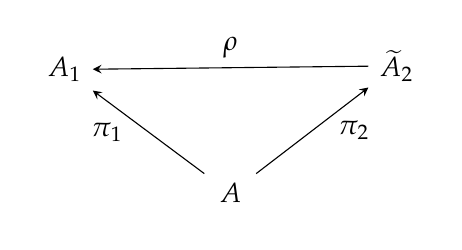
\begin{tikzpicture}
		\matrix (m) [matrix of math nodes,row sep=3em,column sep=4em,minimum width=2em]
		{
			A_1  & & \widetilde{A}_2 \\ 
			& A & \\};
		\path[-stealth]
		(m-1-3) edge node [above] {$\rho$} (m-1-1)
		(m-2-2) edge node [left]  {$\pi_1~~$} (m-1-1)
		(m-2-2) edge node [right] {$~~\pi_2$} (m-1-3);
		\end{tikzpicture}
		\\ 	
	\end{itemize}
	There is the natural equivalence of the categories $A_0:\mathfrak{FinCov}$-$\sX \cong \mathfrak{FinCov}$-$A$.
	
\end{cor}
\begin{proof}
	From the Theorem \ref{ctr_fin_thm} it follows that there is a one-to-one correspondence between objects of $\mathfrak{FinCov}$-$\sX$ and objects of  $\mathfrak{FinCov}$-$A$ given by
	$$
	\left(p:\widetilde{\sX} \to \sX \right) \mapsto 	A_0\left( p\right) :   A_0\left( \sX\right)    \hookto A_0\left( \widetilde{\sX}\right)
	$$
	where $A_0\left(p\right)$ is given by the Definition \ref{ctr_funct_not_defn}. If $p_1:\widetilde{\sX}_1 \to \sX$ and $p_2:\widetilde{\sX}_2 \to \sX$ are objects of $\mathfrak{FinCov}$-$\sX$ and $p: \widetilde{\sX}_1 \to \widetilde{\sX}_2$ is a morphism of $\mathfrak{FinCov}$-$\sX$ then from the Theorem \ref{ctr_fin_thm} it turns out that $p$ is a transitive finite-fold covering. From the equation \ref{ctr_ff_funct_not_eqn} it follows that $p$ corresponds to the *-homomorphism
	\be\label{ctr_c_funct_lem_eqn}
	A_0\left(p \right):  A_0\left( \widetilde{\sX}_2\right)    \to A_0\left( \widetilde{\sX}_1\right).
	\ee
	So one has a functor from  $\mathfrak{FinCov}$-$\sX$ to  $\mathfrak{FinCov}$-$A$. Let us define the inverse  functor. From the Theorem \ref{ctr_fin_thm} it follows that any object $\pi: A_0\left( \sX\right) \hookto A_0\left( \widetilde{\sX}\right)$ of $\mathfrak{FinCov}$-$A$ corresponds to a transitive finite-fold covering $p: \widetilde{\sX} \to \sX$ such that $\pi = A_0\left(p \right)$. If $A_0\left(p_1 \right): A_0\left( {\sX}\right)\to  A_0\left( \widetilde{\sX}_1\right) $ and $A_0\left(p_2 \right): A_0\left( {\sX}\right)\to A_0\left( \widetilde{\sX}_2\right)$ are objects of $\mathfrak{FinCov}$-$A$  and $\pi: A_0\left( \widetilde{\sX}_2\right)    \to A_0\left( \widetilde{\sX}_1\right)$ is a *-homomorphism such that $A_0\left(p_1\right) = \pi \circ A_0\left(p_2\right)$ then $\pi$ corresponds to a continuous map $p: \widetilde{\sX}_1 \to \widetilde{\sX}_2$ such than $p_1= p \circ p_2$. So one has the inverse functor from   $\mathfrak{FinCov}$-$A$ to $\mathfrak{FinCov}$-$\sX$.
\end{proof}






\subsection{Coverings of operator spaces}
\begin{empt}\label{ctr_fin_op_empt}
Let $\left(X, Y\right)$ be a  {sub-unital subspace} having continuous trace (cf. Definition \ref{ctr_oa_defn}) and let $A\bydef C^*_e\left(X, Y \right)$ be the $C^*$-envelope of $\left(X, Y\right)$. From the Lemma  \ref{ctr_oa_lem} it follows that $A$ has continuous trace, hence the spectrum $\sX$ of $A$ is the locally compact Hausdorff space. Let $p: \widetilde \sX \to \sX$ be a transitive covering, denote by
\be\label{ctr_fin_op_eqn}
\begin{split}
\widetilde X \stackrel{\text{def}}{=} C_0\left(\lift_p\left[X\right]\right),\\
\widetilde A \stackrel{\text{def}}{=}  C_0\left(\lift_p\left[A\right]\right)= A_0\left(\widetilde \sX \right) \quad \text{ (cf. Equation \ref{ctr_ff_funct_not_eqn})} ,\\
\widetilde Y \stackrel{\text{def}}{=} \widetilde X + \C \cdot 1_{\widetilde A^+}.
\end{split}
\ee
(cf. Equations \ref{top_c0_eqn}, \ref{top_cont_s_lift_eqn}).
If the covering $p$ is finite-fold then there are the natural injective *-homomorphism $\rho: A \to \widetilde A$ and the complete unital  isometry $\left(\pi_X, \pi_Y \right):  \left(X, Y \right) \hookto \left(\widetilde X, \widetilde Y \right)$ from $ \left(X, Y \right)$ to  $\left(\widetilde X, \widetilde Y \right)$ (cf. Definition \ref{op_sum_space_defn}).
\end{empt}
 

\begin{theorem}\label{ctr_fin_op_thm}
Let us consider the given by \ref{ctr_fin_op_empt} situation. If $\sX$ is a connected, locally connected and second-countable space then there is the 1-1 map from the set of finite-fold transitive coverings $p: \widetilde\sX \to\sX$ 
\eqref{fin_op_defn} and noncommutative  finite-fold  coverings of the subunital operator space $\left(X, Y\right)$ given by
\bea\label{ctr_from_oa_eqn}
\left(p: \widetilde\sX \to\sX \right) \mapsto \left(\left(X, Y \right),\left(\widetilde X, \widetilde Y \right), G\left(\left.\widetilde\sX \right|\sX\right), \left(\pi_X, \pi_Y \right) \right).
\eea 
\end{theorem}
\begin{proof}
	Firstly we proof that $\left(\left(X, Y \right),\left(\widetilde X, \widetilde Y \right), G\left(\left.\widetilde\sX \right|\sX\right), \left(\pi_X, \pi_Y \right) \right)$ is a finite-fold  covering  for each transitive finite-fold covering $p: \widetilde\sX \to\sX$. One needs check (a) and (b) of the Definition \ref{fin_op_defn}.\\
(a)	From the Theorem \ref{ctr_fin_thm} it turns out that
	$$
	\left( C^*_e\left( X,  Y \right), \widetilde{A}, G\left(\left.\widetilde\sX \right|\sX\right), C_0\left(p \right)  \right)
	$$  a finite-fold  noncommutative covering. From $X_x \subset A_x$ for any $x \in \sX$, $\widetilde X_{\widetilde x}\cong X_{p\left( \widetilde x\right) }$ and $\widetilde A_{\widetilde x}\cong A_{p\left( \widetilde x\right) }$ it follows that $C_0\left(\widetilde X_{\widetilde x}, \widetilde Y_{\widetilde x} \right) = \rep_{ \widetilde{x}}\left(\widetilde{A}\right)$ for all $\widetilde{x}\in \widetilde{\sX}$ (cf. notation of the Definition \ref{ctr_oa_defn}).
	Applying  the Lemma \ref{ctr_oa_lem} one has $\widetilde A = C^*_e\left(\widetilde X, \widetilde Y \right)$, clearly the following condition holds $\pi_Y = \left.\rho\right|_Y$, $\pi_X = \left.\rho\right|_X$.\\
(b)
If $\widetilde X' \subset C^*_e\left(\widetilde X, \widetilde Y \right)$ is a $\C$-linear space  such that $X = \widetilde X' \cap  C^*_e\left( X,  Y \right)$ and $G\widetilde X'= \widetilde X'$ then from $\widetilde X_{ \widetilde x }\cong X_{p\left( \widetilde x\right) }$ it follows that $\widetilde X'_{ \widetilde x }\subset \widetilde X_{ \widetilde x }$ for all $ \widetilde x \in \widetilde \sX$.  From the Lemma \ref{top_sub_eq_lem} it follows that $\widetilde X' \subset\widetilde X$.

Secondly  we proof that any noncommutative finite-fold  covering $$\left(\left(X, Y \right),\left(\widetilde X, \widetilde Y \right), G, \left(\pi_X, \pi_Y \right) \right)$$  of the subunital operator space $\left(X, Y\right)$ yields  the transitive finite-fold covering $p: \widetilde\sX \to\sX$. From  (a) of the Definition \ref{fin_op_defn} it follows that $$\left(\left(X, Y \right),\left(\widetilde X, \widetilde Y \right), G, \left(\pi_X, \pi_Y \right) \right)$$ corresponds to noncommutative covering $\left( C^*_e\left( X,  Y \right), C^*_e\left(\widetilde X, \widetilde Y \right), G, \rho \right)$ of $C^*$-algebras. However  $C^*_e\left( X,  Y \right)$ has continuous trace, so and taking into account the Theorem \ref{ctr_fin_thm} on can find required covering $p: \widetilde \sX\to \sX$.
\end{proof}

\subsection{Induced representation}\label{ctr_induced_finite_sec}
\paragraph*{} 
Let us consider a compact  Riemannian manifold $M$ with a spinor bundle $S$. The algebra $C\left(M \right) \otimes \mathbb{M}_n\left(\C \right)$ is a homogeneous of order $n$ $C^*$-algebra (cf. Definition \ref{ctr_homo_defn}). If $p: \widetilde M \to M$ is a finite-fold transitive covering then from the Theorem \ref{ctr_fin_thm} it follows that there is a noncommutative finite-fold covering
\be\label{ctr_act_declr_eqn}
\left(C\left(M \right) \otimes \mathbb{M}_m\left(\C \right), C\left(\widetilde M~ \right) \otimes \mathbb{M}_m\left(\C \right), G\left(\left.\widetilde M \right| M\right) \right) 
\ee
If  $\varphi_{\mathrm{fin}}:\mathbb{M}_m\left( \C\right) \to B\left( \C^k\right)$ is a faithful representation then there is the action
\be
\begin{split}
C\left(M \right) \otimes \mathbb{M}_m\left(\C \right)\times C\left(M, \left\{\sS_x\otimes \C^k\right\}, \Ga\left(M, \sS \right) \otimes \C^k \right) \to\\\to C\left(M, \left\{\sS_x\otimes \C^k\right\}, \Ga\left(M, \sS \right) \otimes \C^k \right)
\end{split}
\ee
such that from
\bean
a = a' \otimes T,  \quad a' \in C\left(M \right) \quad T \in \mathbb{M}_m\left(\C \right),\\
\xi = \xi' \otimes x, \quad \xi' \in \Ga\left(M, \sS \right) \quad x \in \C^k
\eean
it follows that
$$
a \xi = a' \xi' \otimes \varphi_{\mathrm{fin}}\left(T \right)x  
$$
There is the alternative description of the above action. The $C^*$-algebra $C\left(M \right) \otimes \mathbb{M}_m\left(\C \right)$ is a continuity structure for $M$ and the family $\left\{\mathbb{M}_m\left(\C \right)_x\right\}_{x \in \sX}$ such that
$$
C\left(M \right) \otimes \mathbb{M}_m\left(\C \right)\cong C\left(M,\left\{\mathbb{M}_m\left(\C \right)_x\right\}, C\left(M \right) \otimes \mathbb{M}_m\left(\C \right) \right) 
$$
For any $x \in \sX$ the representation $\varphi_{\mathrm{fin}}$ induces the action $\mathbb{M}_m\left(\C \right)_x\times \sS_x\otimes \C^k \to \sS_x\otimes \C^k$ such that
\be\label{ctr_act_eqn}
a_x \left(s_x\otimes y  \right) = s \otimes \varphi_{\mathrm{fin}}\left( a_x\right) y, \quad \forall a_x \in \mathbb{M}_m\left(\C \right)_x, \quad \forall s_x \in \sS_x, \quad \forall y \in \C^k.
\ee
If $a \in C\left(M,\left\{\mathbb{M}_m\left(\C \right)_x\right\}, C\left(M \right) \otimes \mathbb{M}_m\left(\C \right) \right)$ corresponds to a family $\left\{a_x \in \mathbb{M}_m\left(\C \right)\right\}_{x \in \sX}$ and $\xi \in C\left(M, \left\{\sS_x\otimes \C^k\right\}, \Ga\left(M, \sS \right) \otimes \C^k \right)$ is corresponds to a family $\left\{\xi_x \in \sS_x \otimes \C^k\right\}_{x \in \sX}$ then the product $a \xi$ corresponds to the family $\left\{a_x\xi_x \in \sS_x \otimes \C^k\right\}_{x \in \sX}$ where the action \eqref{ctr_act_eqn} is implied. From the Lemma \ref{top_homo_c_lem} it follows that there is the following isomorphism
\be\label{ctr_fin_iso_eqn}
\begin{split}
\left( C\left(\widetilde M\right) \otimes \mathbb{M}_m\left(\C \right)\right)\otimes_{C\left( M \right) \otimes \mathbb{M}_m\left(\C \right)}
\\\otimes_{C\left( M \right) \otimes \mathbb{M}_m\left(\C \right)}\left( C\left(M, \left\{\sS_x\otimes \C^k\right\}, \Ga\left(M, \sS \right) \otimes \C^k \right)\right) \xrightarrow{\approx}\\
\xrightarrow{\approx}\lift_p\left[\left( C\left(M, \left\{\sS_x\otimes \C^k\right\}, \Ga\left(M, \sS \right) \otimes \C^k \right)\right)\right]
\end{split}
\ee
of left $C\left(\widetilde M\right) \otimes \mathbb{M}_m\left(\C \right)$-modules.
Note that  $\sS_x\otimes \C^k \cong \sS^k_x$ and taking into account Lemmas \ref{top_bundle_cs_lem} and \ref{top_lift_bundle_lem} the given by \eqref{ctr_fin_iso_eqn} isomorphism can be represented by the following way
\be\label{ctr_gfin_iso_eqn}
\begin{split}
	\left( C\left(\widetilde M\right) \otimes \mathbb{M}_m\left(\C \right)\right)\otimes_{C\left( M \right) \otimes \mathbb{M}_m\left(\C \right)}
\Ga\left(M, \sS^k \right) \xrightarrow{\approx}
\Ga\left(\widetilde M, \widetilde\sS^k \right)
\end{split}
\ee
where $\widetilde\sS$ is the inverse image of $\sS$. For any $x \in \sX$ the space $\sS_x$ is a Hilbert space, so $\sS^k_x = \sS_x \otimes\C^k$ has the natural structure of Hilbert space which is the finite direct product of Hilbert spaces. It follows that $\sS^k$ is a {Hermitian vector bundle} (cf. Definition \ref{top_herm_bundle_defn}) and $L^2\left(M, \sS^k \right)\cong  L^2\left(M, \sS \right)^k$ is a Hilbert space with the given by \eqref{top_bundle_herm_scalar_eqn} scalar product, i.e.
\be\label{ctr_bundle_herm_scalar_eqn}
\left( \xi, \eta\right)_{L^2\left(M, S^k\right)}\stackrel{\text{def}}{=} \int_{M}\left( \xi_x, \eta_x\right)_xd\mu.
\ee
\begin{lemma}\label{ctr_hilb_homo_lem}
If $p: \widetilde{M} \to M$ is a finite-fold  transitive covering and $\widetilde{\SS}$ is the {inverse image} of $\SS$ by $p$ (cf. Definition \ref{vb_inv_img_funct_defn}) then the following conditions hold:
	\begin{itemize}
		\item [(i)] The map \eqref{ctr_gfin_iso_eqn} can be extended up to the following homomorphism 
		$$
	\left( C\left(\widetilde M\right) \otimes \mathbb{M}_m\left(\C \right)\right)\otimes_{C\left( M \right) \otimes \mathbb{M}_m\left(\C \right)}
L^2\left(M, \sS^k \right) \xrightarrow{\approx}
L^2\left(\widetilde M, \widetilde\sS^k \right)
		$$
		of left $C\left(\widetilde M\right) \otimes \mathbb{M}_m\left(\C \right)$-modules.
		\item[(ii)] The image of $\left( C\left(\widetilde M\right) \otimes \mathbb{M}_m\left(\C \right)\right)\otimes_{C\left( M \right) \otimes \mathbb{M}_m\left(\C \right)}
		L^2\left(M, \sS^k \right)$ is dense in $L^2\left(\widetilde M, \widetilde\sS^k \right)$.
	\end{itemize}
\end{lemma}
\begin{proof}
There is the natural inclusion of $C^*$-algebras
\bean 
C\left(\widetilde M\right)\to C\left(\widetilde M\right) \otimes \mathbb{M}_m\left(\C \right),\\
\widetilde a \mapsto \widetilde  a \otimes 1_{\mathbb{M}_m\left(\C \right)}.
\eean
Using it one can prove this lemma as well as the Lemma \ref{top_hilb_homo_lem} had been proved.
\end{proof}
\begin{remark}
	Indeed the image of $C\left(\widetilde M\right)\otimes_{C\left(M\right)} L^2\left(M, \sS\right)$ coincides with $L^2\left(\widetilde{M}, \widetilde{\SS} \right)$. However this fact is not used here.
\end{remark}
Let both $\mu$ and $\widetilde{\mu}$ be Riemannian measure (cf.  \cite{do_carmo:rg}) on both $M$ and $\widetilde{M}$ respectively which correspond to both the volume element (cf. \eqref{top_vol_eqn}) and its $p$-lift (cf. \eqref{top_vol_lift_eqn}).
If $ A \bydef  C\left({M} \right)\otimes \mathbb{M}_m\left(\C \right)$, $\widetilde A \bydef  C\left(\widetilde{M} \right)\otimes \mathbb{M}_m\left(\C \right)$ and
$\widetilde{a} \otimes \xi, \widetilde{b} \otimes \eta \in \widetilde A \otimes_{A}  \Ga\left( M, \sS^k\right) \subset L^2\left(\widetilde{M},\widetilde{\sS}^k \right)$  then  the given by the Equation \eqref{induced_prod_equ} scalar product $\left(\cdot, \cdot \right)_{\text{ind}}$ on  $\widetilde A \otimes_{A}  \Ga\left( M, \sS^k\right)$ satisfies to the following equation
\begin{equation}\label{ctr_ind_l2_eqn}
\begin{split}
\left( \widetilde{a} \otimes \xi ,    \widetilde{b} \otimes \eta\right)_{\text{ind}}= \left(\xi, \left\langle \widetilde{a}, \widetilde{b}\right\rangle_{C\left(\widetilde{M} \right) } \eta \right)_{L^2\left({M},{\sS}^k \right)}=\\=\sum_{\widetilde{\a}\in \widetilde{\mathscr A}}\left(\xi, \left\langle \widetilde{a}_{\widetilde{\a}}\widetilde{a}, \widetilde{b}\right\rangle_{C\left(\widetilde{M} \right) } \eta \right)_{L^2\left({M},{\sS}^k \right)}
= \sum_{\widetilde{\a}\in \widetilde{\mathscr A}}\left(\xi, \mathfrak{desc}\left( \widetilde{a}_{\widetilde{\a}} \widetilde{a}^* \widetilde{b}\right)  \eta \right)_{L^2\left({M},{\sS}^k \right)}=
\\
=
\sum_{\widetilde{\a}\in \widetilde{\mathscr A}}~\int_M \left(\xi_x, \mathfrak{desc}\left( \widetilde{a}_{\widetilde{\a}} \widetilde{a}^* \widetilde{b}\right)  \eta_x \right)_x d\mu=
\\
=
\sum_{\widetilde{\a}\in \widetilde{\mathscr A}}~\int_M \left(\mathfrak{desc}\left( \widetilde{e}_{\widetilde{\a}} \widetilde{a}\right)\xi_x, \mathfrak{desc}\left( \widetilde{e}_{\widetilde{\a}}  \widetilde{b}\right)  \eta_x \right)_x d\mu=
\\
=\sum_{\widetilde{\a}\in \widetilde{\mathscr A}}~ \int_{\widetilde{M}}\left(\widetilde{a} \lift_{\widetilde{\sU}_{\widetilde{\a}}}\left({e}_{\widetilde{\a}}\xi \right)_{\widetilde{x}},  \widetilde{b} ~\lift_{\widetilde{\sU}_{\widetilde{\a}}}\left({e}_{\widetilde{\a}}\eta \right)_{\widetilde{x}}\right)_{\widetilde{x}}d \widetilde{   \mu} =
\\
=\sum_{\widetilde{\a}\in \widetilde{\mathscr A}}~ \int_{\widetilde{M}}\widetilde{a}_{\widetilde{\a}}\left(\widetilde{a} \lift_{\widetilde{\sU}_{\widetilde{\a}}}\left(\xi \right)_{\widetilde{x}},  \widetilde{b} ~\lift_{\widetilde{\sU}_{\widetilde{\a}}}\left(\eta \right)_{\widetilde{x}}\right)_{\widetilde{x}}d \widetilde{   \mu} =
\\
= \int_{\widetilde{M}}\left( \widetilde{a} \lift_p\left(\xi \right)_{\widetilde{x}},  \widetilde{b} ~\lift_p\left(\eta \right)_{\widetilde{x}}\right)_{\widetilde{x}}d \widetilde{   \mu}
= \left( \widetilde{a}~ \lift_p\left(\xi \right),  \widetilde{b} ~\lift_p\left(\eta \right)\right)_{L^2\left(\widetilde{M},\widetilde{\sS}^k \right)} =\\
=  \left(\phi\left(  \widetilde{a}\otimes\xi\right) ,  \phi \left( \widetilde{b}\otimes\eta\right)\right)_{L^2\left(\widetilde{M},\widetilde{\sS}^k \right)}
\end{split} 
\end{equation}
where $\phi$ is given by \eqref{top_atensor_comact_iso}.
The equation \eqref{ctr_ind_l2_eqn} means that $\left(\cdot, \cdot \right)_{\text{ind}}= \left(\cdot, \cdot \right)_{L^2\left(\widetilde{M},\widetilde{\sS}^k \right)}$, and taking into account the dense inclusion $C\left(\widetilde{M} \right) \otimes_{C\left(M \right) } \Ga\left( M, \sS^k\right) \subset L^2\left(\widetilde{M},\widetilde{\sS}^k \right)$ with respect to the Hilbert norm of $L^2\left(\widetilde{M},\widetilde{\sS}^k\right) $
one concludes that the space of induced representation coincides with $L^2\left(\widetilde{M},\widetilde{\sS}^k\right)$. It means that induced representation $C\left(\widetilde{M}\right) \times L^2\left(\widetilde{M},\widetilde{\sS}^k \right) \to L^2\left(\widetilde{M},\widetilde{\sS}^k \right)$ is given by \eqref{comm_bundle_repr_eqn}. So one has the following lemma.
\begin{lemma}\label{ctr_ind_lem}
	If $C\left(M \right)	 \otimes \mathbb{M}_m\left(\C \right)\to B\left(  L^2\left(M,\sS^k \right)\right)$ is the described above representation and
 the representation  $\widetilde{\rho}: C\left(\widetilde{M}\right) \otimes \mathbb{M}_m\left(\C \right)\to  B\left( \widetilde{   \H}\right)  $ is induced by the pair $$
	\left(\rho ,\left(C\left(M \right)  \otimes \mathbb{M}_m\left(\C \right), C\left( \widetilde{M}\right)  \otimes \mathbb{M}_m\left(\C \right), G\left( \left.\widetilde{M}~\right|M\right) \right)  \right)
	$$ 
	(cf. Definition \ref{induced_repr_defn}) then following conditions holds
	\begin{enumerate}
		\item[(a)] There is the homomorphism of Hilbert spaces $\widetilde{   \H}\cong L^2\left(\widetilde{M},\widetilde{\sS}^k \right)$,
		\item[(b)] The representation $\widetilde{\rho}$ is described above action of $C\left(\widetilde{M}\right)\otimes \mathbb{M}_m\left(\C \right)$ on $ L^2\left(\widetilde{M},\widetilde{\sS}^k \right)$.
	\end{enumerate}
\end{lemma}
\begin{proof}
	(a) Follows from \eqref{ctr_ind_l2_eqn},\\
	(b) From the Lemma \ref{ctr_hilb_homo_lem}  it follows that the map \\		$	\left( C\left(\widetilde M\right)\otimes\mathbb{M}_m\left(\C \right)\right) \otimes_{C\left(M\right)\otimes \mathbb{M}_m\left(\C \right)} L^2\left(M, \sS^k\right) \xrightarrow{\approx} L^2\left(\widetilde{M}, \widetilde{\SS}^k \right)$ is the homomorphism of left $C\left(\widetilde M\right)\otimes\mathbb{M}_m\left(\C \right)$ modules, so the given by \eqref{comm_bundle_repr_eqn}, i.e. $C\left(\widetilde M\right)\otimes\mathbb{M}_m\left(\C \right)$-action coincides with the $C\left(\widetilde M\right)\otimes\mathbb{M}_m\left(\C \right)$-action  the given by \eqref{ind_act_form_eqn}.
\end{proof}

\begin{remark}\label{ctr_ind_rem}
	If the spectral triple 
	$$
\widetilde T\bydef	\left( \Coo\left(\widetilde M\right) \otimes \mathbb{M}_m\left(\C \right), L^2\left(\widetilde M, \widetilde S \right)\otimes\C^k,\widetilde \Dslash\otimes \Ga_{\mathrm{fin}}+ \Id_{L^2\left(\widetilde M, \widetilde S \right)} \otimes D_{\mathrm{fin}}\right)	$$ is the {geometrical} $p$-{lift} of the spectral triple 
	$$
	\left( \Coo\left( M\right) \otimes \mathbb{M}_m\left(\C \right), L^2\left(M, S \right)\otimes\C^k, \Dslash\otimes \Ga_{\mathrm{fin}}+ \Id_{L^2\left(M, S \right)} \otimes D_{\mathrm{fin}}\right).
	$$
	 (cf. Definition \ref{ctr_geom_lift_defn}), then clearly the corresponding to $\widetilde T$ representation of $C\left(M \right)\otimes \mathbb{M}_m\left(\C \right)$ equals to the given by the Lemma \ref{ctr_ind_lem} representation.
\end{remark}



\subsection{Coverings of spectral triples}\label{ctr_d_sec}
\paragraph*{}
Consider the situation of the Section \ref{ctr_induced_finite_sec}. Here the notation of the Section \label{top_d_sec} is used. Clearly one has

\be\label{ctr_el_dec_eqn}
C\left( M\right) \otimes \mathbb{M}_m\left(\C \right)\cong \bigoplus_{\substack{r = 1\\s = 1}}^m C\left( M\right)\otimes \mathfrak{e}_{rs}
\ee
where $\mathfrak{e}_{rs}$ are elementary matrices (cf. Definition \ref{elementary_defn}).


\begin{lemma}\label{ctr_smooth_matr_lem}

Let $p:\widetilde M \to M$ be a finite-fold transitive covering. Consider the given by the Corollary \ref{comm_comm_cor} unital finite-fold noncommutative coverings
\bean
\left(C\left(M \right) , C\left(\widetilde M~ \right) , G\left(\left.\widetilde M \right| M\right) \right),\\
\eean
given the Corollary \ref{comm_comm_cor}. If the family $\left\{	\widetilde{e}_{\widetilde\a}\right\}_{\widetilde\a \in \widetilde{ \mathscr A}}\subset \Coo\left(\widetilde M \right) $ is  the given by \eqref{top_te_eqn} and
\be\label{ctr_fin_set_eqn}
\left\{	\widetilde{e}_{\widetilde\a}\otimes \mathfrak{e}_{rs}\right\}_{\widetilde\a \in \widetilde{ \mathscr A};~r,s =1,...,m}\subset \Coo\left( M\right) \otimes \mathbb{M}_m\left(\C \right)
\ee
then the following conditions hold
\ref{top_smooth_matr_lem}
	\begin{itemize}
		\item[(i)]
		The finite family \eqref{ctr_fin_set_eqn}  satisfies to the Lemma \ref{smooth_matr_lem}.
		\item[(ii)] 
		\be\label{ctr_smooth_lcond_eqn}
		\begin{split}
		C\left(\widetilde M \right) \otimes \mathbb{M}_m\left(\C \right) \cap \mathbb{M}_{m^2\left|\widetilde{\mathscr A}~ \right|}\left(\Coo\left( M\right)\otimes \mathbb{M}_m\left(\C \right)\right) =
		\\
		= \Coo\left(\widetilde M \right)\otimes\mathbb{M}_m\left(\C \right). 
		\end{split}
		\ee
		\item[(iii)] The  given by the the Theorem \ref{ctr_fin_thm} unital
		 noncommutative finite-fold covering $$
\left(C\left(M \right) \otimes \mathbb{M}_m\left(\C \right), C\left(\widetilde M~ \right) \otimes \mathbb{M}_m\left(\C \right), G\left(\left.\widetilde M \right| M\right) \right)		 
		 $$  is smoothly invariant (cf. Definition \ref{smooth_defn}).
	\end{itemize}
\end{lemma}
\begin{proof}
	(i)
	For any $\widetilde{a} \in C\left( \widetilde{M}\right)$ from \eqref{top_te_eqn} it follows that
		$$
	C\left( \widetilde{M}\right) = \sum_{ \widetilde{\a}\in \widetilde{\mathscr A}}\widetilde{e}_{\widetilde\a}C\left(M\right).
	$$
	and taking into account \eqref{ctr_el_dec_eqn} one has
	\bean
	C\left( M\right) \otimes \mathbb{M}_m\left(\C \right)\cong \sum_{\substack{r = 1\\s = 1}}^m \sum_{ \widetilde{\a}\in \widetilde{\mathscr  A}}\left( \widetilde{e}_{\widetilde\a} \otimes \mathfrak{e}_{rs}\right)  C\left( M\right)\otimes \mathbb{M}_m\left(\C \right)
	\eean
	i.e. the right $C\left(M \right)\otimes \mathbb{M}_m\left(\C \right)$ -module $C\left( \widetilde{M}\right)\otimes \mathbb{M}_m\left(\C \right)$ is generated by the finite set \eqref{ctr_fin_set_eqn}.
	Let us prove that the family \eqref{ctr_fin_set_eqn} satisfies to conditions (a) and (b) of the Lemma \ref{smooth_matr_lem}.
	\begin{enumerate}
		\item [(a)]
		From the proof of the Lemma \ref{ctr_smooth_matr_lem} it turns out that
			$$
		\left\langle \widetilde{e}_{\widetilde{\a'}}, \widetilde{e}_{\widetilde{\a''}}\right\rangle_{C\left(\widetilde{M} \right) }= \sum_{g \in  G\left( \left.\widetilde{M}~\right|M\right)} g\left(\widetilde{e}^*_{\widetilde{\a'}}, \widetilde{e}_{\widetilde{\a''}} \right)\in \Coo\left( M\right) 
		$$
		for all $\widetilde{\a'}, \widetilde{\a''}\in \widetilde{\mathscr  A}$, and taking into account that elements $1_{C\left( \widetilde{M}\right)}\otimes  \mathfrak{e}_{rs}$ are $G\left( \left.\widetilde{M}~\right|M\right) $-invariant  one has
	\bean
	\left\langle \widetilde{e}_{\widetilde{\a'}}\otimes  \mathfrak{e}_{rs}, \widetilde{e}_{\widetilde{\a''}}\otimes  \mathfrak{e}_{vw}\right\rangle_{C\left(\widetilde{M} \right) )\otimes \mathbb{M}_m\left(\C \right)}=		\left\langle \widetilde{e}_{\widetilde{\a'}}, \widetilde{e}_{\widetilde{\a''}}\right\rangle_{C\left(\widetilde{M} \right) }\otimes \mathfrak{e}_{rs}\mathfrak{e}_{vw}\in \\ \in\Coo\left( M\right)\otimes \mathbb{M}_m\left(\C \right).
\eean
		\item[(b)]  From the Lemma \ref{top_smooth_matr_lem} it follows that the given by \eqref{top_te_eqn}  family $\left\{	\widetilde{e}_{\widetilde\a}\right\}_{\widetilde\a \in \widetilde{ \mathscr A}}$ is $G\left(\left.\widetilde{M}~\right|M\right)$-invariant, hence the  family \eqref{ctr_fin_set_eqn} is also $G\left(\left.\widetilde{M}~\right|M\right)$-invariant.
	\end{enumerate}
	(ii) If the following condition holds 
	$$
	\widetilde a \otimes b \in C\left(\widetilde M \right)\otimes \mathbb{M}_m\left(\C \right)  \cap \mathbb{M}_{m^2\left| \widetilde{\mathscr  A}\right| }\left(\Coo\left( M\right) \otimes \mathbb{M}_m\left(\C \right) \right)
	$$
then from (i) of the  Lemma \ref{smooth_matr_lem} it follows that
\bean
	\left\langle \widetilde{e}_{\widetilde{\a'}}\otimes  \mathfrak{e}_{rs},	\left( \widetilde a \otimes b\right)  \widetilde{e}_{\widetilde{\a''}}\otimes  \mathfrak{e}_{vw}\right\rangle_{C\left(\widetilde{M} \right) )\otimes \mathbb{M}_m\left(\C \right)}\in \Coo\left( M\right) \otimes \mathbb{M}_m\left(\C \right);\\\forall \widetilde{\a'}, \widetilde{\a''}\in \widetilde{\mathscr  A}, \quad \forall r,s,w,v = 1,...,m.
\eean
	On the other hand from \eqref{ctr_el_dec_eqn} it follows that
\be\label{ctr_rs_eqn}
	\widetilde a \otimes b = \sum_{\substack{r = 1\\s = 1}}^m \widetilde a_{rs}\otimes \mathfrak{e}_{rs},
\ee
so one has
\be\label{ctr_matr_eqn}
\begin{split}
	\left\langle \widetilde{e}_{\widetilde{\a'}}\otimes  \mathfrak{e}_{rr},	\left( \widetilde a \otimes b\right)  \widetilde{e}_{\widetilde{\a''}}\otimes  \mathfrak{e}_{ss}\right\rangle_{C\left(\widetilde{M} \right) )\otimes \mathbb{M}_m\left(\C \right)}= 	\left\langle \widetilde{e}_{\widetilde{\a'}}, \widetilde a_{rs}  \widetilde{e}_{\widetilde{\a''}}\right\rangle_{C\left(\widetilde{M} \right)}\otimes \mathfrak{e}_{rs}\in\\\in\Coo\left( M\right) \otimes \mathbb{M}_m\left(\C \right).
\end{split}
\ee
From \eqref{ctr_matr_eqn} and the Lemma \ref{ctr_smooth_matr_lem} it follows that $\widetilde a_{rs} \in \Coo\left(\widetilde M\right)$ and taking into account \eqref{ctr_rs_eqn} following condition holds
$$
\widetilde a \otimes b \in \Coo\left(\widetilde M\right) \otimes \mathbb{M}_m\left(\C \right),
$$
i.e.
\bean
C\left(\widetilde M \right)\otimes \mathbb{M}_m\left(\C \right)  \cap \mathbb{M}_{m^2\left| \widetilde{\mathscr  A}\right| }\left(\Coo\left( M\right) \otimes \mathbb{M}_m\left(\C \right) \right) \subset \Coo\left(\widetilde M\right) \otimes \mathbb{M}_m\left(\C \right).
\eean
Conversely if  $\widetilde a \otimes b \in \Coo\left(\widetilde M\right) \otimes \mathbb{M}_m\left(\C \right)$ and $\widetilde a \otimes b$ is given by \eqref{ctr_rs_eqn} then following condition holds
\be\label{ctr_matrp_eqn}
\begin{split}
	\left\langle \widetilde{e}_{\widetilde{\a'}}\otimes  \mathfrak{e}_{rs},	\left( \widetilde a \otimes b\right)  \widetilde{e}_{\widetilde{\a''}}\otimes  \mathfrak{e}_{vw}\right\rangle_{C\left(\widetilde{M} \right) )\otimes \mathbb{M}_m\left(\C \right)}= 	\left\langle \widetilde{e}_{\widetilde{\a'}}, \widetilde a_{sv}  \widetilde{e}_{\widetilde{\a''}}\right\rangle_{C\left(\widetilde{M} \right)}\otimes \mathfrak{e}_{rs}\mathfrak{e}_{vw}.
\end{split}
\ee
On the other hand from the Lemma \ref{ctr_smooth_matr_lem} it follows that $\left\langle \widetilde{e}_{\widetilde{\a'}}, \widetilde a_{sv}  \widetilde{e}_{\widetilde{\a''}}\right\rangle_{C\left(\widetilde{M} \right)}\in \Coo\left(M\right)$, hence $\left\langle \widetilde{e}_{\widetilde{\a'}}\otimes  \mathfrak{e}_{rs},	\left( \widetilde a \otimes b\right)  \widetilde{e}_{\widetilde{\a''}}\otimes  \mathfrak{e}_{vw}\right\rangle_{C\left(\widetilde{M} \right) )\otimes \mathbb{M}_m\left(\C \right)}\in \Coo\left(\widetilde M\right) \otimes \mathbb{M}_m\left(\C \right)$, and taking into account \eqref{ctr_rs_eqn} one has
$$
\widetilde a \otimes b \in \Coo\left(\widetilde M\right) \otimes \mathbb{M}_m\left(\C \right),
$$
i.e.
$$
\Coo\left(\widetilde M\right) \otimes \mathbb{M}_m\left(\C \right)\subset C\left(\widetilde M \right)\otimes \mathbb{M}_m\left(\C \right)  \cap \mathbb{M}_{m^2\left| \widetilde{\mathscr  A}\right| }\left(\Coo\left( M\right) \otimes \mathbb{M}_m\left(\C \right) \right) .
$$
	(iii) From (ii) the  Lemma \ref{smooth_matr_lem}. 
\end{proof}
Consider the given by \eqref{ctr_sp_tr_prod_sec} product of spectral triples
\bean
\left( \Coo\left( M\right) \otimes \mathbb{M}_m\left(\C \right), L^2\left(M, S \right)\otimes\C^k, \Dslash\otimes \Ga_{\mathrm{fin}}+ \Id_{L^2\left(M, S \right)} \otimes D_{\mathrm{fin}}\right) 
\eean
and let $D$ be an unbounded operator on $L^2\left(M, S \right)\otimes\C^k$ given by
\be\label{ctr_d_eqn}
D = \Dslash\otimes \Ga_{\mathrm{fin}}+ \Id_{L^2\left(M, S \right)} \otimes D_{\mathrm{fin}}.
\ee
From the evident equations
\bean
\left[D, a \otimes 1_{\mathbb{M}_m\left(\C \right)}\right]= \left[\Dslash, a \right]\otimes \Ga_{\mathrm{fin}}\quad \forall a \in \Coo\left( M\right), \\
\left[D, 1_{C\left(\widetilde M\right)} \otimes b\right]= \Id_{L^2\left(M, S \right)} \otimes \left[D_{\mathrm{fin}}, b\right]\quad \forall b \in \mathbb{M}_m\left(\C \right).
\eean
it follows that 
\be
\left[\Dslash, a \right]\otimes \Ga_{\mathrm{fin}}, ~ \Id_{L^2\left(M, S \right)} \otimes \left[D_{\mathrm{fin}}, b\right] \in \Om^1_D;\quad \forall a \in \Coo\left( M\right)\quad \forall  b \in \mathbb{M}_m\left(\C \right).
\ee
where $\Om^1_D\subset B\left( L^2\left(M, S \right)\otimes\C^k\right)$ is  the {module of differential forms associated} with the spectral triple \eqref{ctr_sp_tr_prod_sec} (cf. Definition \ref{ass_cycle_defn}).
Similarly to \eqref{top_atensor_s_comact_iso} one can define a $\Coo\left(\widetilde M \right)$-module  homomorphism
\be\label{ctr_phinf_eqn}
\begin{split}
	\phi_\infty :	C^\infty\left(\widetilde M\right) \otimes\mathbb{M}_n\left(\C \right) \otimes_{	C^\infty\left( M\right) \otimes\mathbb{M}_n\left(\C \right)} \Ga^\infty\left(M,\sS\right) \xrightarrow{\approx}\Ga^\infty\left(\widetilde M, \widetilde\sS\right);\\
	\sum_{j=1}^m \widetilde a_j \otimes\xi_j \mapsto \widetilde a_j\lift_p\left(\xi_j \right). 
\end{split}
\ee
where both   $\Ga^\infty\left(M, \sS \right)$ and $\Ga^\infty\left(\widetilde M, \widetilde\sS \right)$ are  defined by the Equations  \eqref{top_smooth_m_eqn} and \eqref{top_lift_sheaf_eqn} respectively.
\begin{lemma}\label{ctr_phinf_lem}
	The given by the Equation \eqref{top_phinf_eqn} homomorphism is an isomorphism.
\end{lemma}
\begin{proof}
	The proof of the Lemma \ref{top_tensor_comact_lem} uses the partition of unity. However from the Proposition \ref{smooth_part_unity_prop} it turns out that there is a smooth partition of unity. Using it one can proof this lemma as well as the Lemma \ref{top_tensor_comact_lem} has been proved.
\end{proof}

Now we have  the  $G\left( \left.\widetilde{M}~\right|M\right)$-{equivariant} connection $\widetilde\nabla$, so on can find the specialization of explained in  \ref{triple_conn_lift_empt} construction of the operator
$\widetilde{D} : \widetilde{\A} \otimes_{\A} \H^\infty \to \widetilde{\A} \otimes_{\A} \H^\infty$. Following table reflects the mapping between general theory and the commutative specialization\\ \\
\begin{tabular}{|c|c|c|}
	\hline
	&General theory & Commutative specialization\\ 
	\hline
	&	&\\
	Hilbert spaces & $\H$  and $\widetilde\H$ &  $L^2\left(M, \sS \right)^k$ and $L^2\left(\widetilde M, \widetilde \sS \right)^k$\\ & & \\
	Pre-$C^*$-algebras	& $\A$  & $\Coo\left(M \right)\otimes\mathbb{M}_n\left(\C \right)$   \\  
&$\widetilde\A$ & $\Coo\left(\widetilde M \right)\otimes\mathbb{M}_n\left(\C \right)$   \\ & & \\
	Dirac operators & $D$ & $\Dslash\otimes \Ga_{\mathrm{fin}}+ \Id_{L^2\left(M, S \right)^k} \otimes D_{\mathrm{fin}}$  \\
	& $\widetilde{D}$ & ?\\  & & \\
	&$\H^\infty\bydef \bigcap_{n =1}^\infty \Dom D^n\subset \H$ & $\Ga^\infty\left(M, \sS \right)^k= \bigcap_{n =1}^\infty \Dom D^n$ \\& & \\
	\hline
\end{tabular}
\\
\\
\\

Let 	$\widetilde{\slashed{\nabla}}: \Coo\left(\widetilde{M} \right) \to \Coo\left(\widetilde{M} \right) \otimes_{\Coo\left({M} \right)}\Om^1_{\slashed D}$ be a given by \eqref{top_nabla_eqn} $G\left( \left.\widetilde{M}~\right|M\right)$-{equivariant} connection (cf. \eqref{equiv_conn_eqn}). 
Suppose that $\widetilde{a}\in\Coo\left(\widetilde{M} \right)$ and 
$$
\widetilde{\slashed{\nabla}}\left(\widetilde{a} \right) = \sum_{j=1}^r\widetilde{a}_j\otimes \left[\Dslash, a_j \right]  \in \Coo\left(\widetilde{M} \right) \otimes_{\Coo\left({M} \right)}\Om^1_{\slashed D}
$$
Denote by
\be\label{ctr_nabla_eqn}
\begin{split}
	\widetilde{{\nabla}}: \Coo\left(\widetilde{M} \right) \otimes \mathbb{M}_m\left(\C \right)\to \Coo\left(\widetilde{M} \right)\otimes \mathbb{M}_m\left(\C \right) \otimes_{\Coo\left({M} \right)\otimes \mathbb{M}_m\left(\C \right)}\Om^1_{D},\\
	\widetilde a \otimes b \mapsto %\sum_{j=1}^r\left( \widetilde{a}_j \otimes b\right) \otimes\left(  \left[\Dslash, a_j \right]\otimes \Ga_{\mathrm{fin}} \right) +
	%+ \left( \widetilde a \otimes 1_{\mathbb{M}_m\left(\C \right)}\right)\otimes \left( \Id_{L^2\left(M, S \right)} \otimes \left[D_{\mathrm{fin}}, b\right]\right)=\\
	\sum_{j=1}^r\left(  \widetilde{a}_j\otimes  \left[\Dslash, a_j \right]\right) \otimes b\Ga_{\mathrm{fin}}  +
	\widetilde a \otimes \left[D_{\mathrm{fin}}, b\right].
\end{split}
\ee
From $\left[D_{\mathrm{fin}}, bb'\right] = b \left[D_{\mathrm{fin}}, b'\right]+\left[D_{\mathrm{fin}}, b\right]b'$, $\Ga_{\mathrm{fin}}b' = b'\Ga_{\mathrm{fin}}$ and
$
\widetilde{\slashed{\nabla}}\left(\widetilde{a} a\right) = \widetilde{\slashed{\nabla}}\left(\widetilde{a} \right)a+ \widetilde{a}\left[\Dslash, a\right], \quad \forall a \in \Coo\left({M} \right)
$
it follows that for any $b' \in \mathbb{M}_m\left(\C \right)$ one has
\bean
\widetilde{{\nabla}}\left(\left(\widetilde a \otimes b \right) \left( a \otimes b' \right) \right)=
\\
=\left(\sum_{j=1}^r\left(  \widetilde{a}_j\otimes  \left[\Dslash, a_j \right]\right) a+ \widetilde a\otimes \left[\Dslash, a\right]  \right)\otimes bb'\Ga_{\mathrm{fin}} +
\widetilde a a\otimes \left[D_{\mathrm{fin}}, bb'\right]=\\
= \left(\sum_{j=1}^r\left(  \widetilde{a}_j\otimes  \left[\Dslash, a_j \right]\right)a   \right)\otimes b\Ga_{\mathrm{fin}}b'+ \widetilde a a\otimes \left[D_{\mathrm{fin}}, b\right]b'+
\\
+\left( \widetilde a\otimes \left[\Dslash, a\right]\right) \otimes b\Ga_{\mathrm{fin}}b'+  \widetilde aa\otimes b\left[D_{\mathrm{fin}}, b'\right].
\eean
From \eqref{ctr_nabla_eqn} it follows that
$$
\left(\sum_{j=1}^r\left(  \widetilde{a}_j\otimes  \left[\Dslash, a_j \right]\right)a   \right)\otimes b\Ga_{\mathrm{fin}}b'+ \widetilde a a\otimes \left[D_{\mathrm{fin}}, b\right]b' = \widetilde{{\nabla}}\left(\widetilde a \otimes b \right) \left( a \otimes b' \right) 
$$
and taking into account that
$$
\left( \widetilde a\otimes \left[\Dslash, a\right]\right) \otimes b\Ga_{\mathrm{fin}}b'+  \widetilde aa\otimes b\left[D_{\mathrm{fin}}, b'\right]=\left(\widetilde a \otimes b \right)\otimes\left[ D, a \otimes b' \right]
$$
we conclude that
$$
\widetilde{{\nabla}}\left( \left(\widetilde a \otimes b \right) \left( a \otimes b' \right)\right) = \widetilde{{\nabla}}\left(\widetilde a \otimes b \right) \left( a \otimes b' \right)+  \left(\widetilde a \otimes b \right) \left[D, a \otimes b'\right],
$$
i.e. $\widetilde{{\nabla}}$ is a connection (cf. \eqref{conn_triple_eqn}). 
The connection 	$\widetilde{\slashed{\nabla}}$ is  $G\left( \left.\widetilde{M}~\right|M\right)$-{equivariant}, so $\widetilde{{\nabla}}$ is also  $G\left( \left.\widetilde{M}~\right|M\right)$-{equivariant} (cf. \eqref{equiv_conn_eqn}).
Let us find the specialization of the operator $\widetilde D$ given by the equation \ref{d_defn_eqn}. If $\xi \otimes \eta \in L^2\left( M, S\right)\otimes \C^k$ then the from \ref{d_defn_eqn} and \eqref{ctr_nabla_eqn} it follows that
\bean
\widetilde D\left(\left(\widetilde a \otimes b \right)\otimes \left(\xi \otimes \eta\right) \right) = \sum_{j=1}^r\left(  \widetilde{a}_j\otimes  \left[\Dslash, a_j \right]\xi\right) \otimes b\Ga_{\mathrm{fin}}\eta  +
\left( \widetilde  a\otimes \xi\right)  \otimes \left[D_{\mathrm{fin}}, b\right]\eta+\\
+\left(\widetilde a \otimes b  \right) \otimes D\left(\xi\otimes \eta \right).
\eean
Taking into account \eqref{ctr_d_eqn} one has 
$
\left(\widetilde a \otimes b  \right) \otimes D\left(\xi\otimes \eta \right)= \left( \widetilde a \otimes \Dslash\xi \right) \otimes b\Ga_{\mathrm{fin}}\eta  + \left( \widetilde a \otimes \xi\right) \otimes b D_{\mathrm{fin}}\eta
$  it turns out that
\be\label{ctr_sub1_eqn}
\begin{split}
\widetilde D\left(\left(\widetilde a \otimes b \right)\otimes \left(\xi \otimes \eta\right) \right)= \\
=\widetilde D\left(\left(\widetilde a \otimes \xi \right)  \otimes b\eta \right)=\sum_{j=1}^r\left(  \widetilde{a}_j\otimes  \left[\Dslash, a_j \right]\xi\right) \otimes b\Ga_{\mathrm{fin}}\eta  +
\left( \widetilde  a\otimes \xi\right)  \otimes \left[D_{\mathrm{fin}}, b\right]\eta+\\
+ \left( \widetilde a \otimes \Dslash\xi \right) \otimes b\Ga_{\mathrm{fin}}\eta  + \left( \widetilde a \otimes \xi\right) \otimes b D_{\mathrm{fin}}\eta=\\
=\left( \sum_{j=1}^r \widetilde{a}_j\otimes  \left[\Dslash, a_j \right]\xi+  \widetilde a \otimes \Dslash\xi\right) \otimes b\Ga_{\mathrm{fin}}\eta +  \left( \widetilde a\otimes \xi \right) \otimes \left(\left[D_{\mathrm{fin}}, b\right]+  bD_{\mathrm{fin}}\right) \eta=\\
=\left(  \sum_{j=1}^r \widetilde{a}_j\otimes  \left[\Dslash, a_j \right]\xi+  \widetilde a \otimes \Dslash\xi\right) \otimes b\Ga_{\mathrm{fin}}\eta +  \left( \widetilde a\otimes \xi \right) \otimes D_{\mathrm{fin}} b\eta.
\end{split}
\ee
However from \eqref{top_d_det_eqn} it follows that
\be\label{ctr_sub2_eqn}
\begin{split}
 \sum_{j=1}^m \widetilde{a}_j\otimes  \left[\Dslash, a_j \right]~ \Rightarrow~ \sum_{j=1}^m \widetilde{a}_j\otimes  \left[\Dslash, a_j \right]\xi + \widetilde a \otimes \Dslash\xi =p^{-1}{\slashed D}\left(\widetilde a \otimes \xi \right) 
\end{split}
\ee
where  $p^{-1}\Dslash$ is the   $p$-{inverse image} of $\Dslash$ (cf. Definition \ref{top_smooth_inv_im_defn} and Equation \ref{top_mo_eqn}). Substitution of \eqref{ctr_sub2_eqn} into right part of  \eqref{ctr_sub1_eqn} gives the following
\bean
\widetilde D\left(\left(\widetilde a \otimes \xi \right)  \otimes b\eta \right)=p^{-1}{\slashed D}\left(\widetilde a \otimes \xi \right) \otimes \Ga_{\mathrm{fin}}b\eta + \left( \widetilde a\otimes \xi \right) \otimes D_{\mathrm{fin}}b\eta,
\eean
or equivalently
\be\label{ctr_pmo_f_eqn}
\widetilde D = p^{-1}\Dslash\otimes \Ga_{\mathrm{fin}}+ \Id_{L^2\left(\widetilde M, \widetilde\sS \right)} \otimes D_{\mathrm{fin}}.
\ee



\begin{thm}\label{ctr_fin_sp_tr_thm} 
	Consider the situation of the Definition \ref{ctr_geom_lift_defn}, i.e.
\begin{itemize}
	\item The spectral triple
	$$
	\mathrm{T } = \left( \Coo\left( M\right) \otimes \mathbb{M}_m\left(\C \right), L^2\left(M, S \right)\otimes\C^k, \Dslash\otimes \Ga_{\mathrm{fin}}+ \Id_{L^2\left(M, S \right)\otimes\C^k} \otimes D_{\mathrm{fin}}\right).
	$$
	\item The regular finite-fold covering $p : \widetilde M\to M$.
	\item The  given by 
		$$
\widetilde{\mathrm{T}} = 	\left( \Coo\left(\widetilde M\right) \otimes \mathbb{M}_m\left(\C \right), L^2\left(\widetilde M, \widetilde S \right)\otimes\C^k,\widetilde \Dslash\otimes \Ga_{\mathrm{fin}}+ \Id_{L^2\left(\widetilde M, \widetilde S \right)\otimes\C^k} \otimes D_{\mathrm{fin}}\right) 
	$$
	{geometrical} $p$-{lift} of  $	\mathrm{T }$.
\end{itemize}
The  {geometrical} $p$-{lift} of $	\mathrm{T }$ (cf. Definition \ref{ctr_geom_lift_defn}) coincides with the\\ $\left(C\left(M \right) \otimes \mathbb{M}_m\left(\C \right), C\left( \widetilde{M}\right)\otimes \mathbb{M}_m\left(\C \right) , G\left( \left.\widetilde{M}~\right|M\right)   \right)$-lift of $T$ (cf. Definition \ref{triple_conn_lift_defn}). 
\end{thm}
\begin{proof}
	Denote by $\left(\widetilde \A, \widetilde\H, \widetilde D\right)$ the\\ $\left(C\left(M \right)\otimes \mathbb{M}_m\left(\C \right) , C\left( \widetilde{M}\right) \otimes \mathbb{M}_m\left(\C \right), G\left( \left.\widetilde{M}~\right|M\right)  \right)$-lift of $	\mathrm{T }$. Consider the given by \eqref{ctr_fin_set_eqn} finite set. 
	From (iii)	of the Lemma \ref{ctr_smooth_matr_lem} it turns that\\ $\left(C\left(M \right)\otimes \mathbb{M}_m\left(\C \right) , C\left( \widetilde{M}\right)\otimes \mathbb{M}_m\left(\C \right) , G\left( \left.\widetilde{M}~\right|M\right)\right)$ is  smoothly invariant. According to the Definition \ref{triple_conn_lift_defn} and taking into account the Equation \eqref{ctr_smooth_lcond_eqn} one has
	\bean
	\widetilde \A =		C\left(\widetilde M \right) \otimes \mathbb{M}_m\left(\C \right) \cap \mathbb{M}_{m^2\left|\widetilde{\mathscr A}~ \right|}\left(\Coo\left( M\right)\otimes \mathbb{M}_m\left(\C \right)\right) =
	\\
	= \Coo\left(\widetilde M \right)\otimes\mathbb{M}_m\left(\C \right). 
	\eean 
	If $\rho: C\left(M \right)\otimes\mathbb{M}_m\left(\C \right)\to L^2\left(M, S \right)\otimes\C^k$ is the representation of the spectral triple 
	$T$ then the representation $\widetilde \rho: C\left(\widetilde M \right)\otimes \mathbb{M}_m\left(\C \right)\to B\left(\widetilde \H \right)$ of the spectral triple  $\left(\widetilde \A, \widetilde\H, \widetilde D\right)$ is induced by the pair\\ $\left(\rho,\left(C\left(M \right) \otimes \mathbb{M}_m\left(\C \right), C\left( \widetilde{M}\right)\otimes \mathbb{M}_m\left(\C \right) , G\left( \left.\widetilde{M}~\right|M\right)   \right)  \right)$. From the Remark \ref{ctr_ind_rem} it follows that the representation $\widetilde \rho$ is equivalent to the  representation, which corresponds to the spectral triple $T$. From \eqref{ctr_pmo_f_eqn} it follows that 
	$$
\widetilde D = p^{-1}\Dslash\otimes \Ga_{\mathrm{fin}}+ \Id_{L^2\left(\widetilde M, \widetilde\sS \right)^k} \otimes D_{\mathrm{fin}}
	$$ and taking into account \eqref{top_ds_eqn} one has $\widetilde{\Dslash}= p^{-1}{\Dslash}$ we conclude that the spectral triple  $\left(\widetilde \A, \widetilde\H, \widetilde D\right)$  is equivalent to the $\widetilde{	\mathrm{T }}$ one.
	\end{proof}

\subsection{Unoriented spectral triples}\label{ctr_sp_tr} 
\paragraph*{}
Consider the described in the Section \ref{comm_sp_tr} situation, i.e. one has

\begin{itemize}
	\item The Riemannian manifold $\widetilde M$ with the spinor bundle $\widetilde\SS$ such that there is the spectral triple $\left(\Coo\left(\widetilde{M},  \right) , L^2\left(\widetilde{M},\widetilde{\sS} \right), \widetilde\Dslash \right)$.
	\item The unoriented Riemannian manifold $M$ with the two listed covering $p:\widetilde M\to M$ and the bundle $\SS \to M$ such that $\widetilde{\sS}$ is the $p$-inverse image of $\SS$.
	\item The unoriented spectral triple $\left(\Coo\left({M},  \right) , L^2\left({M},{\sS} \right), \Dslash \right)$ given by the Theorem \ref{com_unori_thm}
\end{itemize}

\begin{theorem}\label{ctr_unori_thm}
In the described above situation there is the given by
	\be\label{ctr_equ}
	\left(\Coo\left(M \right) \otimes\mathbb{M}_m\left(\C \right) , L^2\left({M}, {\SS}\right)^k, \slashed D \otimes \Ga_{\mathrm{fin}}+ \Id_{L^2\left( M, \sS \right)^k} \otimes D_{\mathrm{fin}} \right).
	\ee
 unoriented spectral triple (cf. Definition \ref{unoriented_defn}).
\end{theorem}
\begin{proof}
	The following table shows the specialization of  objects 1-5 required by the Definition \ref{unoriented_defn}. 
	\\ \\
	\begin{tabular}{|c|c|c|}
		\hline
		&Definition \ref{unoriented_defn} & This theorem specialization\\ 
		\hline
		&	&\\
		1 & $\A$   &  $\Coo\left(M \right)\otimes\mathbb{M}_m\left(\C \right)$ \\ & & \\
		2	& $\left(A, \widetilde A, \Z_2\right)$ & $\left(C\left(M \right)\otimes\mathbb{M}_m\left(\C \right), C\left(\widetilde M\right)\otimes\mathbb{M}_m\left(\C \right), \Z_2 \right)$   \\  & & \\
		3 & $\rho: A \to B\left(\H \right)$ & $C\left(M \right)\otimes\mathbb{M}_m\left(\C \right)\to B\left( L^2\left({M}, {\SS}\right)^k\right) $  \\ & & \\
		4	& $D$ & $\slashed D \otimes \Ga_{\mathrm{fin}}+ \Id_{L^2\left( M, \sS \right)^k} \otimes D_{\mathrm{fin}}$ \\  & & \\
		5	& $\left(\widetilde{\A}, \widetilde{\H}, \widetilde{D} \right)$ & $	\left(\Coo\left(\widetilde M \right) \otimes\mathbb{M}_m\left(\C \right) , L^2\left(\widetilde{M}, \widetilde{\SS}\right)^k, \widetilde D  \right)$ \\
		&& where $\widetilde D \bydef \widetilde\Dslash \otimes \Ga_{\mathrm{fin}}+ \Id_{L^2\left(\widetilde M, \widetilde\sS \right)^k} \otimes D_{\mathrm{fin}}$\\ && \\
		\hline
	\end{tabular}
	\\
	\\
	\\
	Similarly to the proof of the Theorem \ref{com_unori_thm} one can proof that above objects satisfy to the conditions (a)-(d) of the Definition \ref{unoriented_defn}.
\end{proof}




\section{Infinite coverings}\label{ctr_case_sec}
\subsection{Coverings of $C^*$-algebras}

\begin{lemma}\label{ctr_t_a_lem}
		Let $A$ be a separable $C^*$-algebra with continuous trace let $\sX = \hat A$ be the spectrum of $A$. Suppose that $\sX$ is a connected, locally connected, second-countable space.
	Let us consider the situation \ref{comm_t_a_empt} and suppose that 
	\bean
	A \bydef C_0\left(\sX, \left\{A_x\right\}_{x \in \sX}, A \right)
	\eean
	 and $A_0$ is the given by the  Definition \ref{top_c_funct_defn} functor.
	Following conditions hold:
	\begin{enumerate}
		\item[(i)] 	If
		$
		\mathfrak{S}_{ \mathcal{X} } = \left\{p_{\la}:\mathcal{X}_\la \to  \mathcal{X}  \right\}_{\la \in \La}\in \mathfrak{FinTop}
		$
		is  a  topological  finite covering category (cf. Definition \ref{top_sec_defn}) then there is the natural  algebraical  finite covering category (cf. Definition \ref{comp_defn}).
		\begin{equation*}
		\mathfrak{S}_{A } = \left\{\pi_\la=A_0\left( p_{\la}\right) :A  \hookto A_0\left( \mathcal{X}_\la\right) \right\}_{\la \in \La}\in \mathfrak{FinAlg}.
		\end{equation*}
		\item[(ii)] Conversely any directed algebraical  finite covering category
		\begin{equation}
		\mathfrak{S}_{A } = \left\{ \pi_{\la} :A  \hookto A_0\left( \mathcal{X}_\la\right) \right\}_{\la \in \La}\in \mathfrak{FinAlg}.
		\end{equation}
		naturally induces 
		directed topological  finite covering category $$
		\mathfrak{S}_{\mathcal{X}} = \left\{p_{\la}:\mathcal{X}_\la \to \mathcal{X}\right\}_{\la \in \La}\in \mathfrak{FinTop}.$$
		
	\end{enumerate}
	
\end{lemma}
\begin{proof}
	(i)
	One needs check the conditions (a) and (b) of the Definition \ref{comp_defn}.
\begin{enumerate}
	\item[(a)] 	The conditions (a)-(d) of the Definition \ref{compliant_covering_defn}  directly follow from (a)-(d) of the Lemma \ref{comm_comply_lem}.
	\item[(b)] Follows from the Corollary \ref{ctr_functor_cor}.
	
	

\end{enumerate}	
	(ii) From the Theorem \ref{ctr_fin_thm} it turns out that any object $ \pi_\la :A  \hookto A_0\left( \mathcal{X}_\la\right)$ of the category $\mathfrak{S}_{A }$ corresponds to the object $p_\la: \sX_\la \to \sX$ of the category $\mathfrak{S}_{ \mathcal{X}}$, i.e. $p_\la$ is a transitive finite-fold covering. If $\mu, \nu \in \La$ are such that $\mu > \nu$ then from (b) of the Definition \ref{comp_defn} it follows that there is *-homomorphism $\pi: A_0\left( \mathcal{X}_\nu\right)\to A_0\left( \mathcal{X}_\mu\right)$ such that 
	\be\label{ctr_inf_pp_eqn}
	A_0\left( p_\mu\right)= \pi \circ A_0\left( p_\nu\right).
	\ee
	From (a) of the Definition \ref{comp_defn} it turns out that the homomorphism $\pi$ is a noncommutative  finite fold covering, so taking into account the Corollary \ref{ctr_functor_cor} one has the topological finite-fold covering $p: \mathcal{X}_\mu\to \mathcal{X}_\nu$ such that $\pi = A_0\left(p\right)$. From \eqref{ctr_inf_pp_eqn} it follows that $p_\mu = p \circ p_\nu$.
\end{proof}

\begin{lemma}\label{ctr_base_point_lem}
	If	$\mathfrak{S}_{\left(\sX, x_0\right)}= \left\{p_\la:\left( \sX_\la, x^\la_0\right) \to \left( \sX, x_0\right)\right\}_{\la \in \La} \in \mathfrak{FinTop}^{\mathrm{pt}}$ is a pointed topological finite covering category such that for any $\mu > \nu$ there is the unique  pointed  covering $p^\mu_{ \nu}: \left(\sX_{\mu}, x^\mu_0 \right) \to \left(\sX_{\nu}, x^\nu_0 \right)$ then
	\be\label{ctr_base_point_eqn}
	\begin{split}
		\mathfrak{S}^{\mathrm{pt}}_{A } = \\
		=\left\{A_0\left( p_\la\right) : A  \hookto A_0\left(\sX_\la \right)\right\}, \left\{A_0\left( p_\nu^\mu\right) : A_0\left(\sX_\nu \right) \hookto A_0\left(\sX_\mu \right)\right\}
	\end{split}
	\ee
	is a {pointed algebraical  finite covering category} (cf. Definition \ref{comp_pt_defn}).
\end{lemma}
\begin{proof}
	According to our construction for any $\mu >\nu$ the category $	\mathfrak{S}_{A }$ contains the unique *-homomorphism from $A_0\left(\sX_\nu \right)$ to $A_0\left(\sX_\mu \right)$. This lemma follows from the Remark \ref{comp_pt_rem}.
\end{proof}

\begin{empt}\label{ctr_implicit_inc_full_empt}
	Consider the specialization of Lemma  \ref{top_atomic_lem} such that $A = \left(\sX, \left\{A_x\right\}_{x \in \sX}, A\right)$, and   $A_0$, and the given by the Lemma \ref{top_atomic_lem} functor.
	Suppose that  $\H_x$ is  the space of the given by \eqref{rep_x_eqn} representation  $\rep_x: A \to B\left(\H_x\right)$ and  $\K\stackrel{\text{def}}{=} \rep_x\left( A\right) $ where $\K = \mathbb{M}_n\left(\C\right)$ or $\K = \K\left( L^2\left(\N \right) \right)$. 
	From the Lemma \ref{ctr_base_point_lem} it follows that \eqref{ctr_base_point_eqn} is the pointed algebraical  finite covering category. 	
	Let $\widehat{A}\stackrel{\text{def}}{=} C^*$-$\varinjlim_{\la \in \La} A_0\left( {\sX}_\la\right)$ the $C^*$-inductive limit, and let $\pi_a:\widehat{A} \hookto B\left(\H_a\right)$ be the atomic representation (cf. Definition \ref{atomic_repr_defn}). If $\overline{A}$ is  the disconnected algebraical inverse noncommutative limit of $\mathfrak{S}^{\mathrm{pt}}_{A }$ (cf. Definition \ref{main_defn_full_defn}) then there is the natural inclusion $\overline{A} \subset B\left(\H_a \right)$. Otherwise $\H_a = \bigoplus_{ \widehat x \in \widehat \sX} \H_{\widehat x}$ where $\widehat\sX$ is the spectrum of $\widehat A$ and $\H_{\widehat x}$ is the space of representation $\rep_{\widehat x}\left(  \widehat A\right) \to B\left( \H_{\widehat x}\right)$. If $\widehat \sX$ is the spectrum of $\widehat A$ then from the Lemma \ref{inverse_lim_sp_lem} it follows that $\widehat \sX = \varprojlim_{\la \in \La}\sX_\la$. Otherwise if $\overline \sX$ is the  disconnected inverse limit of 	$\mathfrak{S}_{\left(\sX, x_0\right)}$ then there is the natural bijective continuous map $\phi:\overline \sX \to \widehat \sX$ if $\widehat p : \widehat \sX \to \sX$ is the natural map and both $\rep_{\overline x} \overline A\to B\left( \H_{\overline x}\right)$, $\rep_{\overline x} \overline A\to B\left( \H_{\overline x}\right)$ are natural irreducible representations then $\H_{\overline x} \cong \H_{\widehat p \circ \phi\left( \overline x\right)}$,   $\H_{\widehat x} \cong \H_{\widehat p \left( \overline x\right)}$, hence $ \H_{\overline x} \cong \H_{\phi\left( \overline x\right)}$ for all $\overline x \in \overline\sX$. So one has
	$$
	\bigoplus_{ \widehat x \in \widehat \sX} \H_{\widehat x}\cong \bigoplus_{ \overline x \in \overline \sX} \H_{\overline x}
	$$
	The left part of the above equation is the space of the atomic representation of $\widehat A$, right part is the space of the atomic representation of $A_0\left(\overline \sX\right)$. So the atomic representation of $A_0\left(\overline \sX\right)$ can be regarded as the natural inclusion 
	\be\label{ctr_ca_inc_eqn}
	\varphi_A: A_0\left(\overline \sX\right)\hookto B\left( \H_a\right).
	\ee
	\end{empt}

\begin{remark}\label{ctr_implicit_inc_full_rem}
	Below the given by the Equation \eqref{ctr_ca_inc_eqn} *-homomorphism will be replaced with the inclusion $A_0\left(\overline \sX\right)\subset B \left( \widehat \H_a\right)$ of $C^*$-algebras.
	Similarly to the Remark \ref{implicit_inc_full_rem}
	below for all $\la\in\La$ we implicitly assume that $A_0\left( \sX_\la\right) \subset  B\left(\H_a \right)$. Similarly the following natural inclusion 
	\bean
	C^*\text{-}\varinjlim_{\la\in\La} A_0\left( \sX_\la\right) \subset B\left(\widehat \H_a\right)
	\eean
	will be implicitly used. These inclusions enable us replace the Equations \ref{spec_a_eps_eqn} with the following equivalent system of equations
	\be\label{ctr_spec_a_eps_imp_eqn}
	\begin{split}
		\sum_{g\in G_\la } z^*\left(  g\overline a\right) z   \in A_0\left( \sX_\la\right) ,\\
		\sum_{g\in G_\la } f_\eps\left(z^*\left(  g\overline a\right) z   \right)   \in A_0\left( \sX_\la\right),\\
				\sum_{g\in G_\la  } \left(z^*\left(  g\overline a\right) z   \right)^2    \in A_0\left( \sX_\la\right). 
	\end{split}
	\ee
	where $G_\la \bydef \ker\left(G\left(\left.\overline\sX\right|\sX\right)\to G\left(\left.\sX_\la\right|\sX\right) \right)$. 
\end{remark}
\begin{example}\label{ctr_implicit_inc_full_exm}
Let $X_{C_0\left(\sX\right)}\bydef  C_0\left(\sX, \left\{\H_x \right\},   X_{C_0\left(\sX\right)}  \right) $ be a Hilbert $C_0\left(\sX \right)$-module given by \eqref{top_c0_hilb_iso_eqn}. If	$\mathfrak{S}_{\left(\sX, x_0\right)}= \left\{p_\la:\left( \sX_\la, x^\la_0\right) \to \left( \sX, x_0\right)\right\}_{\la \in \La} \in \mathfrak{FinTop}^{\mathrm{pt}}$ is a pointed topological finite covering category then for each $\la\in \La$ define
\bean
X_{C_0\left(\sX\right)}\bydef C_0\left(  \lift_{p_\la}\left[ X_{C_0\left(\sX\right)} \right]  \right) 
\eean
	If	$\mathfrak{S}_{\left(\sX, x_0\right)}= \left\{p_\la:\left( \sX_\la, x^\la_0\right) \to \left( \sX, x_0\right)\right\}_{\la \in \La} \in \mathfrak{FinTop}^{\mathrm{pt}}$ is a pointed topological finite covering category  them from the Lemma \ref{ctr_base_point_lem} it follows that there is a {pointed algebraical  finite covering category} (cf. Definition \ref{comp_pt_defn}) given by
		\be\label{ctr_x_base_point_eqn}
	\begin{split}
		\mathfrak{S}^{\mathrm{pt}}_{\K\left(X_{C_0\left(\sX\right)} \right)  } \bydef \\
	\bydef\left\{\left\{\K\left( p_\la\right) : \K\left(X_{C_0\left(\sX\right)} \right) \hookto \K\left(X_{C_0\left(\sX_\la\right)} \right)  \right\},\left\{\K\left( p_\nu^\mu\right)\right\}\right\}
	\end{split}
	\ee
	If $\widehat \K \bydef C^*\text{-}\varinjlim_{\la\in\La} \K\left(X_{C_0\left(\sX_\la\right)} \right)$ and $\widehat \K\hookto B\left(\widehat \H_a \right)$ is the atomic representation then from \ref{ctr_implicit_inc_full_empt} it follows that
	\be\label{ctr_atom_eqn}
\widehat \H_a=	\bigoplus_{ \overline x \in \overline \sX} \H_{\overline x}	
	\ee
	where $\bigoplus$ means the Hilbert norm completion of the algebraic direct sum. 	
\end{example}

  
\begin{lemma}\label{ctr_c0_inc_lem}
	If the spectrum of $A$ is paracompact and locally connected then 
	there is the natural inclusion
	$$
A_0\left( \overline{\sX}\right)\subset  \overline{A}.
	$$
	(cf. Equation \eqref{ctr_ca_inc_eqn}).
\end{lemma}

\begin{proof}
	Denote by	$\overline{p}: \overline{   \mathcal X } \to \sX$ and $\overline{p}_\la: \overline{   \mathcal X } \to \sX_\la$. 
	If $\overline{   \mathcal U } \subset \overline{   \mathcal X }$ is an open set which is homeomorphically mapped onto $\sU = \overline{p}\left(  \overline{   \mathcal U }\right)  \subset \overline{   \mathcal X }$ then $\overline{   \mathcal U }$ is homeomorpfilally mapped onto $\sU_\la = \overline{p}_\la\left(  \overline{   \mathcal U }\right)  \subset \overline{   \mathcal X }_\la$ for any $\la \in \La$. Let $\overline{a} \in A_0\left( \overline{   \mathcal X }\right)_+$ is a positive element such that $\supp \overline{a} \subset  \overline{   \mathcal U }$. Following proof contains two parts:
	\begin{enumerate}
		\item [(i)] Element $\overline{a}$ is special.
		\item[(ii)] 	$ A_0\left( \overline{\sX}\right)\subset  \overline{A}$.
	\end{enumerate}
(i) One needs check that.  $\overline{a}$  satisfies to the  conditions (a), (b) of the Definition  \ref{special_element_defn}.
\begin{enumerate}
	\item[(a)] For any $\eps \ge 0$,  $\la \in \La$ and  $z \in A_{\la}^+$  there is $a^\eps_\la \in A_\la$ one has\\ $\supp z^* \overline az, \supp f_\eps\left(z^* \overline az\right),  \supp \left( z^* \overline az\right)^2 \subset \overline{   \mathcal U }$, so from the Lemma \ref{comm_lift_desc_sum_strong_lem} it turns out that 
	\bean
	\sum_{g\in \ker\left(  \widehat G\to  G\left(\left.\sX_\la~\right|~\sX \right)\right) } g\left(z^* \overline a z\right) = a_\la =   =\desc_{\overline{p}_\la}\left(z^* \overline az\right) \in A_0\left(\sX_\la \right) ,\\ 
	\sum_{g\in \ker\left(  \widehat G\to  G\left(\left.\sX_\la~\right|~\sX \right)\right) } gf_\eps\left(z^* \overline a z\right)    =\desc_{\overline{p}_\la}\left(\ f_\eps\left(z^* \overline az\right) \right) \in A_0\left(\sX_\la \right) ,\\ 
	\sum_{g\in \ker\left(  \widehat G\to  G\left(\left.\sX_\la~\right|~\sX \right)\right) } g\left(z^* \overline a z\right)^2    =b_\la \desc_{\overline{p}_\la}\left(z^* \overline az\right)^2 \in A_0\left(\sX_\la \right)
	\eean
	where the strong convergence of the series is implied. Above equations coincide with \eqref{ctr_spec_a_eps_imp_eqn}.
	
	\item[(b)] 
From $a_\la = \desc_{\overline{p}_\la}\left(z^* \overline az\right)$ and $b_\la = \desc_{\overline{p}_\la}\left(z^* \overline az\right)^2$ it turns out that
$$
	\forall \la  \in \La u  \Rightarrow  \left\|a_\la^2 - b_\la\right\|=0,
$$
i.e. $a_\la$ and  $b_\la$ satisfy the inequality \eqref{special_set_eqn}.
\end{enumerate}
(ii)
Consider a compliant  	{compliant to} the covering  $\overline p:\overline{\mathcal X}\to{\mathcal X}$	partition of unity
\be\nonumber
\sum_{\left( g, \al\right)  \in G\left(\left.\overline{\sX}~\right|\sX\right)\times \mathscr A  } g\overline{\phi}_\a = 1_{C_b\left(\overline{\mathcal X} \right) }
\ee
(cf. Definition \ref{comm_comply_defn})
If $\overline a \in A_0\left( \overline\sX\right)_+$ is any positive element then from the Lemma \ref{ctr_para_sum}	it follows that
$$
\overline a= \sum_{\left( g, \al\right)  \in G\left(\left.\overline{\sX}~\right|\sX\right)\times \mathscr A  } g\overline{\phi}_\a \overline a.
$$
On the other hand it is already proven that $g\overline{\phi}_\a \overline a$ is a special element for all $\left( g, \al\right)  \in G\left(\left.\overline{\sX}~\right|\sX\right)\times \mathscr A$. For any $\eps > 0$ there is a compact set $\overline\sV\subset \overline\sX$ such that $\rep_{ \overline x }\left( \overline a\right) <\eps$ for all $\overline x\in \overline\sX\setminus\overline\sV$ so from the Corollary \ref{top_cfs_cor} it turns out that there is a covering sum 
for $\widetilde\sU$ (cf. Definition \ref{top_cfs_defn}) i.e. a finite subset  $\mathscr A_0 \subset G\left(\left.\overline{\sX}~\right|\sX\right)\times \mathscr A$ such that 
$$
\sum_{\left( g, \al\right) \in \mathscr A_0} g\overline{\phi}_\a\left( \overline x\right) = 1; \quad \forall \overline x \in \overline \sV.
$$
It follows that
$$
\left\|\sum_{\left( g, \al\right) \in \mathscr A_0} g\overline{\phi}_\a \overline a - \overline a \right\| < \eps.
$$
Taking into account that the set $\mathscr A_0$ is finite one has $\sum_{\left( g, \al\right) \in \mathscr A_0} g\overline{\phi}_\a \overline a\in \overline A$ ans since $\eps$ is arbitrary small it turns out that $\overline a\in \overline A$. Thus the positive cone $A_0\left(\overline\sX \right)_+$ of $A_0\left(\overline\sX \right)$ is a subset of $\overline A$. However any $C^*$-algebra is generated by its positive cone, it follows that $A_0\left(\overline\sX \right)\subset\overline A$.
\end{proof}

\begin{empt}
Consider the situation of the Example \ref{ctr_implicit_inc_full_exm}, i.e. $\widehat \K \bydef C^*\text{-}\varinjlim_{\la\in\La} \K\left(X_{C_0\left(\sX_\la\right)} \right)$ and the atomic representation $\widehat \K\hookto B\left(\widehat \H_a \right)$ where
\bean
\widehat \H_a=	\bigoplus_{ \overline x \in \overline \sX} \H_{\overline x}	
\eean
(cf. Equation \eqref{ctr_atom_eqn}).
The space  $X_{C_b\left(\overline \sX \right) }\bydef C_b\left(\lift_{ \overline{p}_{\la}}\left[X_{C_0\left(\sX\right)}\right]\right)$ is a Hilbert $C_b\left(\overline \sX \right)$ - module.
Any bounded family
\be\label{ctr_fam_eqn}
\overline a \bydef \left\{\overline a_{\overline x}\in \K\left(  \H_{\overline x}\right)  \right\}_{ \overline x \in \overline \sX}
\ee
yields a bounded operator in $B\left(\widehat \H_a \right)$. If $X_{D^*\left(\sX\right)}$ is the  \textit{discontinuous extension} of $X_{C_0\left(\sX\right)}$ (cf. Definition \ref{top_disc_ext_defn}) and $\overline\xi\bydef\left\{\overline \xi_{\overline x}\right\}\in X_{D^*\left(\sX\right)}$ then
\be\label{ctr_afam_eqn}
\overline a\overline \xi\bydef\left\{\overline a_{\overline x} \overline \xi_{\overline x}\right\}\in  X_{D^*\left(\sX\right)}
\ee
\end{empt}

\begin{definition}\label{top_coh_defn} 
	Let $\widehat \K\bydef C^*$-$\varinjlim_{\la \in \La} \K\left(X_{C_0\left(\sX_\la\right)}\right)$ be the inductive limit of $C^*$-algebras in sense of the Definition \ref{inductive_lim_non_defn}, and let $\widehat{\pi}_a:\widehat \K \to B\left(\widehat \H_a\right)$ be the atomic representation (cf. Definition \ref{atomic_repr_defn}). Let   $\widehat{G}\bydef \varprojlim_{\la \in \La} G\left(
	\left.  \sX_\la~ \right|\sX\right)$ be the projective limit of groups and let $G_\la \bydef \ker\left(  \widehat G\to  G\left(\left.\sX_\la~\right|~\sX \right)\right)$. 
	An element $\overline a = \left\{\overline a_{\overline x}\in \K\left(  \H_{\overline x}\right)  \right\}_{ \overline x \in \overline \sX}\in B\left(\H_a\right)$ is \textit{coherent}  if for any $\la_0 \in \La$, $\xi_{\la_0} \in X_{\la_0}$
	and  $\eps > 0$ 
	following conditions hold:
	\begin{enumerate}
		\item[(a)] 		If $f_\eps: \R \to \R$ is a continuous function given by \eqref{f_eps_eqn} then
		there are $ f_\la, f^\eps_\la, h_\la, \in C_0\left(\sX_{\la}\right)_+$ such that
		\be\label{top_spec_a_eps_eqn}
		\begin{split}
				\sum_{g\in G_\la } \left\langle \lift_{ \overline{p}_{\la_0}}\left( \xi_{\la_0}\right)g \overline a, \lift_{ \overline{p}_{\la_0}}\left( \xi_{\la_0}\right)\right\rangle_{D^*\left(\overline \sX \right) }    = f_\la,\\
			\sum_{g\in G_\la } f_\eps\left( \left\langle \lift_{ \overline{p}_{\la_0}}\left( \xi_{\la_0}\right) g\overline a, \lift_{ \overline{p}_{\la_0}}\left( \xi_{\la_0}\right) \right\rangle_{D^*\left(\overline \sX \right) }\right)     = f^\eps_\la,\\
			\sum_{g\in G_\la } \left\langle \lift_{ \overline{p}_{\la_0}}\left( \xi_{\la_0}\right)g \overline a, \lift_{ \overline{p}_{\la_0}}\left( \xi_{\la_0}\right) \right\rangle^2_{D^*\left(\overline \sX \right) }    = h_\la. 
		\end{split}
		\ee
		where sums of the above series mean the point-wise convergence, and the Equations \eqref{top_disc_ext_eqn}, \eqref{ctr_afam_eqn} are used.		
		\item[(b)] There is $\mu \in \La$ such that $\mu \ge \la_0$ and
		\be\label{top_special_set_eqn}
		\forall \la  \in \La \quad	 \la \ge \mu  \Rightarrow  \left\|f_\la^2 - h_\la\right\| < \eps
		\ee
		where $a_\la, b_\la \in C_0\left(\sX_{\la}\right)$ are given by \eqref{top_spec_a_eps_eqn}.
	\end{enumerate}
	
\end{definition}


\begin{remark}\label{top_oa_fam_rem}
	Similarly to the Lemma \ref{spec_strong_lim_lem} one can proof that there is the  strong limit $\overline a = \lim \widehat{\pi}_a\left(a'_\la \right)$ in $B\left(\H_a \right)$. It follows that $\overline a$ corresponds to the family
	\be\label{top_oa_fam_eqn}
	\left\{\overline a_{\overline x}\in \H_{\overline x}\right\}_{\overline x\in \overline\sX}.
	\ee
\end{remark}


\begin{lemma}\label{top_coh_lem} 
	Let $\widehat \K\bydef C^*$-$\varinjlim_{\la \in \La} \K\left(X_{C_0\left(\sX_\la\right)}\right)$ be the inductive limit of $C^*$-algebras in sense of the Definition \ref{inductive_lim_non_defn}, and let $\widehat{\pi}_a:\widehat \K \to B\left(\widehat \H_a\right)$ be the atomic representation (cf. Definition \ref{atomic_repr_defn}). Let   $\widehat{G}\bydef \varprojlim_{\la \in \La} G\left(
	\left.  \sX_\la~ \right|\sX\right)$ be the projective limit of groups and let $G_\la \bydef \ker\left(  \widehat G\to  G\left(\left.\sX_\la~\right|~\sX \right)\right)$. Let $\K\left(X_{C_0\left(\sX_\la\right)}\right)$ be given by \eqref{unital_notation_eqn}. 
	If  $\overline a \in B\left( \widehat\H_a\right)$ is such that for any $\la_0 \in \La$, $\eps > 0$ and  $z \in A_{\la_0}^{\sim}$
	it satisfies to the following conditions:	
	\begin{enumerate}
		\item[(a)] 	If   $f_\eps: \R \to \R$ is a continuous function given by \eqref{f_eps_eqn}.
		then for all $\la \ge \la_0$  there are $ a_\la, b_\la, a^\eps_\la \in \K\left(X_{C_0\left(\sX_\la\right)}\right)$ such that
		\be\label{top_o_spec_a_eps_eqn}
		\begin{split}
			\sum_{g\in G_\la } \pi \left(z\right)^*\left(  g\overline a\right) \pi\left( z\right)   = \pi\left(a_\la \right),\\
			\sum_{g\in G_\la } f_\eps\left(\pi \left(z\right)^* \left( g\overline a\right) \pi\left( z\right)\right)    = \pi\left(a^\eps_\la \right),\\
			\sum_{g\in G_\la  } \left(\pi \left(z\right)^* \left( g\overline a\right) \pi\left( z\right)\right)^2    = \pi\left(b_\la \right) 
		\end{split}
		\ee
		where sums of the above series mean the strong convergence in  $B\left( \widehat\H_a\right)$ and the action  $G_\la\times B\left( \widehat\H_a\right)\to B\left( \widehat\H_a\right)$ is given by \eqref{equivb_eqn}.
		\item[(b)] There is $\mu \in \La$ such that $\mu \ge \la_0$ and
		\be\label{top_o_special_set_eqn}
		\forall \la  \in \La \quad	 \la \ge \mu  \Rightarrow  \left\|a_\la^2 - b_\la\right\| < \eps
		\ee
		where $a_\la, b_\la \in A_\la$ are given by \eqref{spec_a_eps_eqn}.
	\end{enumerate}	
	then $\overline a$ is coherent (cf. Definition \ref{top_coh_defn}).
\end{lemma}
\begin{proof}
	Suppose  $\la_0 \in \La$. If $\xi_{\la_0} \in X_{\la_0}$ is an arbitrary element then $z'\bydef \xi_{\la_0}\left\rangle \right\langle \xi_{\la_0}\in \K\left(X_{C_0\left(\sX_{\la_0}\right)}\right)$, such that $\text{norm}_{z'}= \text{norm}^2_{ \xi_{\la_0}}$, i.e. $z'$ is a multiple of $\text{norm}_{ \xi_{\la_0}}$ (cf. Definition \ref{top_multiple_a_defn}).
	From the Lemma \ref{top_multiple_a_lem} it follows that there is $z \bydef \mathfrak{div}\left( z',\text{norm}_{ \xi_{\la_0}}\right)\in \K\left(X_{C_0\left(\sX_{\la_0}\right)}\right)$ (cf. Equation \ref{top_multiple_ad_eqn}). For all  $x \in \sX_{\la_0}$ the dimension of $\rep_x\left(z'\right)$ does not exceed 1, hence $\rep_x\left(z\right)$ also does not exceed 1. Let us check that $\overline a$ satisfies to conditions (a) and (b) of the Definition \ref{top_coh_defn}.
	\begin{enumerate}
		\item [(a)] From \eqref{top_o_spec_a_eps_eqn} it follows that there are $ f_\la, f^\eps_\la, h_\la, \in C_0\left(\sX_{\la}\right)_+$ such that
		\be\label{top_oxt_spec_a_eps_eqn}
		\begin{split}
			\sum_{g\in G_\la }\tr\left( \pi \left(z\right)^*\left(  g\overline a\right) \pi\left( z\right)  \right)  = f_\la ,\\
			\sum_{g\in G_\la }f_\eps\left(\tr\left(\pi \left(z\right)^* \left( g\overline a\right) \pi\left( z\right)\right) \right)    = f^\eps_la,\\
			\sum_{g\in G_\la }\tr\left(\pi \left(z\right)^* \left( g\overline a\right) \pi\left( z\right)\right)^2    = h_\la
		\end{split}
		\ee
		where $\tr\left( \overline b\right)$ means the map $\overline x \mapsto \rep_{\overline x}\left( \overline b\right)$. On the other hand from our construction it follows that 
		\be\label{top_ox_spec_a_eps_eqn}
		\begin{split}
			\tr\left( \pi \left(z\right)^*\left(  g\overline a\right) \pi\left( z\right)  \right)  =  \left\langle \lift_{ \overline{p}_{\la_0}}\left( \xi_{\la_0}\right)g \overline a, \lift_{ \overline{p}_{\la_0}}\left( \xi_{\la_0}\right)\right\rangle_{D^*\left(\overline \sX \right)} ,\\
			f_\eps\left(\tr\left(\pi \left(z\right)^* \left( g\overline a\right) \pi\left( z\right)\right) \right)    =\\
			= f_\eps\left( \left\langle \lift_{ \overline{p}_{\la_0}}\left( \xi_{\la_0}\right)g \overline a, \lift_{ \overline{p}_{\la_0}}\left( \xi_{\la_0}\right)\right\rangle_{D^*\left(\overline \sX \right)}\right) ,\\
			\tr\left(\pi \left(z\right)^* \left( g\overline a\right) \pi\left( z\right)\right)^2    = \left\langle \lift_{ \overline{p}_{\la_0}}\left( \xi_{\la_0}\right)g \overline a, \lift_{ \overline{p}_{\la_0}}\left( \xi_{\la_0}\right)\right\rangle^2_{D^*\left(\overline \sX \right)}
		\end{split}
		\ee
		From the Equations \eqref{top_oxt_spec_a_eps_eqn} and \eqref{top_ox_spec_a_eps_eqn} it turns out that
		\bean
		\begin{split}
			\sum_{g\in G_\la } \left\langle \lift_{ \overline{p}_{\la_0}}\left( \xi_{\la_0}\right)g \overline a, \lift_{ \overline{p}_{\la_0}}\left( \xi_{\la_0}\right)\right\rangle_{D^*\left(\overline \sX \right) }    = f_\la,\\
			\sum_{g\in G_\la } f_\eps\left( \left\langle \lift_{ \overline{p}_{\la_0}}\left( \xi_{\la_0}\right) g\overline a, \lift_{ \overline{p}_{\la_0}}\left( \xi_{\la_0}\right) \right\rangle_{D^*\left(\overline \sX \right) }\right)     = f^\eps_\la,\\
			\sum_{g\in G_\la } \left\langle \lift_{ \overline{p}_{\la_0}}\left( \xi_{\la_0}\right)g \overline a, \lift_{ \overline{p}_{\la_0}}\left( \xi_{\la_0}\right) \right\rangle^2_{D^*\left(\overline \sX \right) }    = h_\la. 
		\end{split}
		\eean
		\item[(b)] From the Equation \eqref{top_o_special_set_eqn} it turns out that
		\bean
		\forall \la  \in \La \quad	 \la \ge \mu  \Rightarrow  \left\|f_\la^2 - h_\la\right\| = \left\|a_\la^2 - b_\la\right\|< \eps.
		\eean
		
		
	\end{enumerate}
	
\end{proof}




\begin{empt}\label{top_pr_empt}
	
	Any element of  $\overline{\xi} \in \ell^2\left(C_b\left(\overline{   \mathcal X} \right)  \right)$ corresponds to a family 
	\be\label{top_xi_fam_eqn}
	\left\{\overline{\xi}\left(\overline{x} \right) \in L^2\left( \N\right)_{\overline{x}} \right\}_{\overline{x}\in \overline{\sX}}.
	\ee
	Similarly any  $\overline{b} \in \K\left( \ell^2\left(C_b\left(\overline{   \mathcal X} \right)  \right)\right)$ corresponds to a family 
	\be\label{top_k_fam_eqn}
	\left\{\overline{b}\left(\overline{x} \right) \in \K\left( L^2\left( \N\right)_{\overline{x}}\right)  \right\}_{\overline{x}\in \overline{\sX}},
	\ee
	hence for any $\overline{x}\in \overline{\sX}$ there is a representation
	\be%\label{top_spec_a_eqn}
	\rho_{\overline{x}}:  \K\left( \ell^2\left(C_b\left(\overline{   \mathcal X} \right)  \right)\right) \to B\left(   L^2\left( \N\right)_{\overline{x}}\right) 
	\ee
	and  there is a faithful representation
	\be
	\rho_{\overline{\sX}}:  \K\left( \ell^2\left(C_b\left(\overline{   \mathcal X} \right)  \right)\right) \hookto B\left( \bigoplus_{\overline{x}\in \overline{\sX}}  L^2\left( \N\right)_{\overline{x}}\right). 
	\ee
	Similarly for any ${x}_\la\in {\sX}_\la$ there is a representation
	\be\label{top_rx_eqn}
	\rho_{{x}_\la}:  \K\left( \ell^2\left(C_b\left({   \mathcal X}_\la \right)  \right)\right) \to B\left(   L^2\left( \N\right)_{{x}_\la}\right) 
	\ee
	and  there is a faithful representation
	\be
	\rho_{{\sX}_\la}:  \K\left( \ell^2\left(C_b\left({   \mathcal X}_\la \right)  \right)\right) \hookto B\left( \bigoplus_{{x}_\la\in {\sX}_\la}  L^2\left( \N\right)_{x_\la}\right). 
	\ee 	 
	From \eqref{top_adj_inc_eqn} it turns out $\K\left(X_{C_0\left(\sX_\la\right)}\right)\subset \K\left(\ell^2\left( {C_0\left(\sX_\la\right)}\right) \right)$ and $\K\left(X_{C_0\left(\sX_\la\right)}\right)$ is a hereditary subalgebra of $\K\left(\ell^2\left( {C_0\left(\sX_\la\right)}\right) \right)$ Taking into account \eqref{top_lift_inc_eqn} and \ref{top_cov_ca_inc}  one has
	\be\label{top_k_l2_hered_eqn}
	\begin{split}
		\K\left(X_{C_0\left(\overline{\sX}\right)}\right)\subset \K\left(\ell^2\left(C_b\left(\overline{   \mathcal X} \right)  \right) \right),\\ \K\left(X_{C_0\left(\overline{\sX}\right)}\right) \text{ is a hereditary subalgebra of } \K\left(\ell^2\left(C_b\left(\overline{   \mathcal X} \right)  \right) \right)
	\end{split}
	\ee
	Denote by $\widehat \K\stackrel{\text{def}}{=} C^*$-$\varinjlim_{\la \in \La} \K\left( X_{C_0\left(\sX_\la\right)}\right)$ the $C^*$-inductive limit in sense of the Definition \ref{inductive_lim_non_defn}. 
	If  $\widehat \pi_a: \widehat \K \hookto B\left(\widehat \H_a\right)$ be the atomic representation (cf. Definition \ref{atomic_repr_defn}). The space $\widehat \H_a$ is the Hilbert direct sum $$
	\widehat \H_a = \bigoplus_{\widehat x \in \widehat\sX} \H_{\widehat x}
	$$
	where $\widehat\sX$ is the spectrum of $\widehat \K$ and $\H_{\widehat x}$ is the irreducible representation which corresponds to ${\widehat x}$ (cf. Definition \ref{equiv_repr_defn}). Similarly to the Lemma \ref{inverse_lim_sp_lem} one can proof that $\widehat \sX$ is homeomorphic the inverse limit of the spectra, i.e. $\widehat\sX = \varprojlim_{\la \in \La} \sX_\la$. Otherwise from the given by the Lemma \ref{top_universal_covering_lem} of the disconnected inverse limit there is the bijective continuous map $\overline \sX \cong\widehat\sX$ and this map gives the following representation of the space 
	\be\label{top_atomic_eqn}
	\widehat \H_a = \bigoplus_{\overline x \in \overline\sX} \H_{\overline x}.
	\ee
	For all $\la\in\La$ the $C^*$-algebra $\K\left( X_{C_0\left(\sX_\la\right)}\right)$ will be regarded as a subalebra of  $\widehat \K$. 
\end{empt}
\begin{lemma}\label{top_z_lem}
	Consider the situation of the (cf. Definition \ref{top_coh_defn}) with the   a coherent element $\overline a \in B\left(\widehat \H_a \right)$. Let $\la_0\in \La$ and $\xi\in X_{C_0\left( \sX_{\la_0}\right) }$. Let $\overline p_{\la_0}: \overline\sX \to \sX_{\la_0}$ be the natural covering, and $\overline\xi\bydef\lift_{ \overline{p}_{\la_0}}\left(\xi \right)\in X_{C_b\left( \overline\sX\right) }$  corresponds to a family $\left\{\overline\xi_{\overline x}\right\}_{\overline x \in \overline\sX}$. If $\overline f : \overline\sX \to \R$ is given by
	\bean
	\overline x \mapsto \left( \overline\xi_{\overline x}, \rep_{\overline x}\left( \overline a\right), \overline\xi_{\overline x} \right) 
	\eean
	then $\overline f\in C_0\left( \overline\sX\right)$.  
\end{lemma}
\begin{proof}
	If $f_\la\in C_0\left(\sX_{\la}\right)$ is given by the equation \eqref{top_spec_a_eps_eqn} and $\overline f_\la \bydef \lift_{ \overline{p}_{\la}}\left(f_\la \right)\in C_b\left(\overline \sX\right)$ then $\overline f= \lim_\la \overline f_\la$ is a point-wise limit. From the Definition \ref{top_coh_defn}  it follows that $\overline f$ satisfies to the Theorem \ref{comm_main_f_thm}, hence $\overline f \in C_0\left(\overline \sX\right)$.
\end{proof}


\begin{corollary}\label{top_coh_cor}
	If $\overline a \in B\left(\H_a\right)$ is coherent (cf. Definition \ref{top_coh_defn}), $\overline{\xi } \in \ell^2\left(C_b\left(\overline{   \mathcal X} \right)\right)$  and
	\bean
	\overline{f}   \in D^*\left( \overline{   \mathcal X}\right),\\
	\overline x \mapsto \left(\overline{\xi }\left( \overline x\right),   \rho_{\overline x}\left( \overline a\right) \overline{\xi }\left( \overline x\right) \right)_{\H_{\overline x}} 
	\eean	
	then $\overline{f}   \in C_b\left( \overline{   \mathcal X}\right)$.
\end{corollary}
\begin{proof}
	From the Lemma \ref{hered_b_lem}  it follows that $X_{C_b\left( \overline{\sX}\right) }$ is the norm completion of $$\ell^2\left(C_b\left( \overline{\sX}\right) \right)\K\left( X_{C_b\left( \overline{\sX}\right) }\right).$$  If $\overline{\xi} \in  \ell^2\left(C_b\left( \overline{\sX}\right)\right) $ then the Lemma \ref{hered_ba_lem} it turns out that for any $\eps > 0$ there is $\overline{\eta} \in X_{C_b\left( \overline{\sX}\right)}$ such that
	\be\label{top_eps_eqn}
	0	 \le \overline{a} \le \K\left(\overline{p}_\la \right)\left( {a}\right) _\la \Rightarrow \left\|\left\langle \overline{\xi} \overline{a}, \overline{\xi} \right\rangle_{C_b\left( \overline{\sX}\right)} - \left\langle \overline{\eta} \overline{a}, \overline{\eta} \right\rangle_{C_b\left( \overline{\sX}\right)}\right\| < \eps.
	\ee
	where $ \K\left(\overline{p}_\la \right)$ is given by \eqref{top_compact_maps_eqn}.
	However form the Lemma \ref{top_z_lem}
	it follows that  $\left\langle \overline\eta \overline{a}, \overline\eta \right\rangle_{C_b\left( \overline{\sX}\right) }\in C_b\left(\overline{\sX} \right)$ and taking into account \eqref{top_eps_eqn} one has $\left\langle \overline{\xi} \overline{a}, \overline{\xi} \right\rangle_{C_b\left( \overline{\sX}\right)} \in C_b\left(\overline{\sX} \right)$. 
\end{proof}
\begin{corollary}\label{top_bound_cor}
	If  $\overline{a} \in B\left( \bigoplus_{\overline{x}\in \overline{\sX}}  L^2\left( \N\right)_{\overline{x}}\right)$ is coherent then
	\be\label{top_coh_cor_eqn}
	\overline{a} \in \K_b\left(X_{C_0\left(\overline{\sX}\right)}\right)= C_b\left( \K\left(X_{C_b\left(\overline{\sX}\right)}\right)\right). 
	\ee
\end{corollary}
\begin{proof}
	If $\overline{\xi} \in \ell^2\left( C_b\left(\overline{\sX} \right)\right)$ then 
	then from the Corollary \ref{top_coh_cor} it turns out that $\left\langle \lift_{\overline{p}_\la} \left(\xi_\la \right) \overline{a}, \lift_{\overline{p}_\la}\left(\xi_\la \right)\right\rangle_{D*\left(\overline{\sX} \right) } \in C_b\left(\overline{\sX} \right)$.
	From the Lemma \ref{comm_exact_lem} and the Corollary \ref{exact_cont_cor} it turns out that  $\overline{a}$ is $C_b\left(\overline{\sX}\right)$-continuous (cf.  Definition  \ref{exact_cont_defn}), so one has $\overline{a} \in \L\left( \ell^2\left(C_b\left(\overline{\sX} \right)  \right) \right)$. The $C^*$-algebra $\K\left( \ell^2\left(C_b\left(\overline{\sX} \right)  \right) \right)$ is a hereditary subalbebra of $\L\left( \ell^2\left(C_b\left(\overline{\sX} \right)  \right) \right)$. Otherwise from $\lift_{ \overline{p}_{\la}} \left(a_\la \right) > \overline{a}$ and $\lift_{ \overline{p}_{\la}} \left(a_\la \right)\in \K\left( \ell^2\left(C_b\left(\overline{\sX} \right)  \right) \right)$ it turns out $\overline{a}\in \K\left( \ell^2\left(C_b\left(\overline{\sX} \right)  \right) \right)$. Taking into account  \eqref{top_k_l2_hered_eqn} $\K\left(X_{C_b\left(\overline{\sX}\right)}\right)$ { is a hereditary subalgebra of } $\K\left(\ell^2\left(C_b\left(\overline{   \mathcal X} \right)  \right) \right)$ and from $\lift_{ \overline{p}_{\la}} \left(a_\la \right)\in \K\left(X_{C_b\left(\overline{\sX}\right)}\right)$ it turns out that
	\be\label{oa_in_kcb_eqn}
	\overline{a} \in \K\left(X_{C_b\left(\overline{\sX}\right)}\right). 
	\ee
	
	
\end{proof}
\begin{lem}\label{top_coh_compact_lem}
	Suppose that $\sX$ is compact.
	If  $\overline{a} \in B\left( \bigoplus_{\overline{x}\in \overline{\sX}}  L^2\left( \N\right)_{\overline{x}}\right)$ is coherent then
	\be\label{top_coh_compact_eqn}
	\overline{a} \in \K_0\left(X_{C_0\left(\overline{\sX}\right)}\right)= C_0\left( \K\left(X_{C_0\left(\overline{\sX}\right)}\right)\right). 
	\ee
\end{lem}
\begin{proof}
	From the Remark \ref{c_misch_rem} it follows that $\overline{a}$ is compact in sense of Mischenko, hence for any $\eps > 0$ from the Lemma 
	\ref{c_misch_a_lem}  it turns out that there is $n \in \N$ such that
	\be\label{top_p_l_p_eqn}
	\left\|\overline{p}_n \overline{a}~ \overline{p}_n - \overline{a}\right\| < \eps.
	\ee
	where $\overline{p}_n\in \K\left( \ell^2\left( C_b\left( \overline{\sX}\right) \right)\right) $ is the projector onto $\oplus_{j=1}^n C_b\left( \overline{\sX}\right)  \subset \ell^2\left(C_b\left( \overline{\sX}\right) \right)$. 
	If $\la_0\in\La$ then since $\sX$ is compact and the covering $\sX_{\la_0}\to\sX$ is finite fold, the space $\sX_{\la_0}$ is compact. It turns out that $C_0\left(\sX_{\la_0} \right)\cong C\left( \sX_{\la_0}\right)$ and $1_{ C\left( \sX_{\la_0}\right)}\in  C\left( \sX_{\la_0}\right)$. 
	Denote by 
	\be\label{com_ap_eqn}
	\begin{split}
		\overline{a}'=\overline{p}_n \overline{a}~\overline{p}_n.
	\end{split}
	\ee
	One has $\overline{a}' \in \K\left(\ell^2\left( C_b\left({\overline\sX}\right) \right) \right)$. 
	If  ${e}_1,..., {e}_n \in 	\ell^2\left( C\left(\sX_{\la_0}\right) \right)$ such that
	$$
	\overline{e}_j = \left(...~, \underbrace{ 1_{C\left(\sX_{\la_0}\right)}}_{j^{\text{th}}-\text{place}}, ..., 0  \right) 
	$$
	and $\overline e_j \bydef \overline p_{\la_0}\left(e_j \right)$ than since the trace of the positive operator equals or exceeds its norm 
	one has
	\be\label{top_xip_eqn}
	\begin{split}
		\left\|\rep_{ \widetilde{x}} \left( \overline{a}'\right) \right\|  \le \sum_{j=1}^n \left\langle \overline{e}_j \overline{a}, \overline{e}_j \right\rangle_{C_b\left(\overline{\sX}\right) }  \left( \widetilde{x}\right) \quad \forall  \widetilde{x}\in  \widetilde{\sX}.
	\end{split}
	\ee
	
	From the Lemma \ref{top_z_lem} it turns out $\left\langle \overline{e}_j \overline{a}, \overline{e}_j \right\rangle_{C_b\left(\overline{\sX}\right) } \in C_0\left(\overline{\sX} \right)$ so 
	\be
	\overline{f}_n =  \sum_{j=1}^n \left\langle \overline{e}_j \overline{a}, \overline{e}_j \right\rangle_{C_b\left(\overline{\sX}\right) } \in C_0\left(\overline{\sX} \right).
	\ee 
	Otherwise from $\overline{a}' \in \K\left(\ell^2\left( C_b\left(\overline{\sX} \right)\right)  \right)$ it turns out 
	$$
	\text{norm}_{\overline{a}}=\left( \overline{x}\mapsto  \left\|\rep_{ \widetilde{x}} \left( \overline{a}'\right) \right\|  \right) \in C_0\left(\overline{\sX} \right),
	$$
	and taking into account  $\overline{f}_n \in C_0\left(\overline{\sX} \right)$, $\text{norm}_{\overline{a}'} \le \overline{f}_n$ one has
	$$
	\text{norm}_{\overline{a}'} \in C_0\left(\overline{\sX} \right). 
	$$
	or equivalently
	$$
	\text{norm}_{p_n\overline{a}p_n} \in C_0\left(\overline{\sX} \right). 
	$$
	From \eqref{top_p_l_p_eqn} it follows that $\text{norm}_{\overline{a}}= \lim_{n \to \infty }\text{norm}_{p_n\overline{a}p_n}$, and taking into account \ref{top_cc0_eqn} it turns out that
	$$
	\overline{a} \in C_0\left(\K\left(X_{C_0\left(\overline{\sX}\right)}\right) \right).
	$$
\end{proof}
\begin{lemma}\label{top_coh_t_lem} Suppose that $\sX$ is a connected, locally connected, locally compact, locally compact, Hausdorff space.
	If  $\overline{a} \in B\left( \bigoplus_{\overline{x}\in \overline{\sX}}  L^2\left( \N\right)_{\overline{x}}\right)$ is coherent then
	\be\label{top_coh_eqn}
	\overline{a} \in \K_0\left(X_{C_0\left(\overline{\sX}\right)}\right)= C_0\left( \K\left(X_{C_0\left(\overline{\sX}\right)}\right)\right). 
	\ee
\end{lemma}
\begin{proof}
	From the Corollary \ref{top_bound_cor} it turns out that there is
	\bean
	\overline f \in C_b\left(\overline \sX\right),\\
	\overline x \mapsto \left\|  \rep_{\overline x}\left( \overline a\right)\right\|
	\eean
	From the construction \ref{top_inv_empt} it follows  that there is the minimal $\la_{\min}\in \La$ such that $\sX_{\la_{\min}}\bydef\sX$. We set $\la_0\bydef  \la_{\min}$. If $a'_{\la_0}\in \K\left(X_{C_0\left(\sX_{\la_0}\right)}\right)$ is given by \eqref{spec_a_eqn} then from the Lemma \ref{ctr_rep_eq_lem} it turns out that for all $\eps > 0$ the set
	\be\label{top_sy_eqn}
	\sY' \bydef \left\{ x\in\sX\left|\left\|  \rep_x\left( a'_{\la_0}\right)\right\| \ge\eps \right.\right\}
	\ee
	is compact. From the Lemmas \ref{fin_comp_lin_lem} and \ref{fin_comp_linl_lem} it follows that there is a connected compact set $\sY \subset \sX$ such that $\sY'\subset\sY$ and $x_0\in \sY$.
Denote by $\sY_{\la_0}\bydef\sY$, $\sY_{\la}\bydef p_\la^{-1}\left( \sY\right)\subset \sX_\la$ and $\overline \sY \bydef \overline p^{-1} \left(\sY\right)\subset\sX$. From $x_0\in \sY$ it turns out that that base-points $x^\la_0$ and $\overline x$  of $\sX_\la$ and  $\overline \sX$ respectively satisfy to the following equations.
	The direct check yields the proof that there is a {pointed topological finite covering category} (cf. Definition \ref{top_sec_p_defn}) $\mathfrak{S}_{\left( \sY, x_0\right) }= \left\{\left( \sY_\la, x^\la_0\right) \to \left( \sY, x_0\right)\right)\}$   with morphisms
	\be\label{top_py_eqn}
	\left.p^\mu_\nu\right|_{\sY_\mu}: \left( \sY_\mu, x^\mu_0\right) \to \left( \sY_\nu, x^\nu_0\right)
	\ee
	Where $p^\mu_\nu: \left( \sX_\mu, x^\mu_0\right) \to \left( \sX_\nu, x^\nu_0\right)$ are morphisms of the {pointed topological finite covering category} $\mathfrak{S}_{\left( \sX, x_0\right) }$. One can consider the family $F = \left\{\K\left(X_{C\left(\sY_\la\right)} \right) \right\}_{\la\in\La}$
	If  $\overline{b} \in B\left( \bigoplus_{\overline{x}\in \overline{\sY}}  L^2\left( \N\right)_{\overline{x}}\right)$ is given by
	\be\label{top_rarb_eqn}
	\rep_{\overline x}\left(\overline b \right) \bydef  \rep_{\overline x}\left(\overline a \right)\quad \forall x \in \overline \sY.
	\ee
	then since $\overline a$ satisfies to the Definition \ref{top_coh_defn}, the element  $\overline b$ also satisfies the to Definition \ref{top_coh_defn}, i.e.  $\overline b$ is coherent with respect to the family $F$. The set $\sY$ is compact so from the Lemmas \ref{top_coh_compact_lem} and  \ref{ctr_rep_eq_lem} it turns out the map   
	\bean
	\overline \sY \to \R,\\
	\overline x \mapsto \left\|  \rep_{\overline x}\left( \overline b\right)\right\| 
	\eean
	lies in $C_0\left(\overline\sX\right)$. The set 
	$$
	\overline \sZ \bydef \left\{\overline x\in\overline\sY\left|\left\|  \rep_{\overline x}\left( \overline b\right)\right\| \ge\eps \right.\right\}
	$$
	is compact. However  $\rep_{\overline x}\left( a'_{\la_0}\right)\ge \rep_{\overline x}\left( \overline a\right)$ for any $\overline x\in \overline\sX$ and taking into account  \eqref{top_sy_eqn} one has
	$$
	\forall \overline x \in \overline\sX \setminus \overline p^{-1} \left(\sY\right)\quad\left\|  \rep_{\overline x}\left( \overline a\right)\right\| < \eps.
	$$
	From the above equation and \eqref{top_rarb_eqn} it follows that 
	$$
	\overline \sZ = \left\{ \overline x\in\overline\sX\left|\left\|  \rep_{\overline x}\left( \overline a\right)\right\| \ge\eps \right.\right\}=  \left\{ x\in\overline\sX\left| \overline f\left( \overline x\right) \ge\eps \right.\right\}.
	$$
	The set  $\overline \sZ$ is compact, hence from the Definition \ref{c_c_def_2} it follows that $	\overline f \in C_0\left(\overline \sX\right)$, and taking into account the  Corollary \ref{top_bound_cor} one has 	$\overline{a} \in C_0\left( \K\left(X_{C_0\left(\overline{\sX}\right)}\right)\right)$. 
	
\end{proof}



\begin{lemma}\label{ctr_spec_inc_lem} 
	Consider the situation of the Lemma \ref{ctr_t_a_lem}.
	If $\overline a \in B\left(\widehat \H_a\right)$ is a special element (cf. Definition \ref{special_element_defn}) then $\overline a \in  A_0\left(\overline\sX \right)$.
\end{lemma}
\begin{proof}
If  $a_\la \in A_0\left(\sX_\la\right)$ is given by \eqref{spec_strong_lim_eqn} then from the Lemma \ref{spec_strong_lim_lem} it follows that $\overline a = \lim_{\la \in \La}\pi_a\left(a_\la \right)$.
	Let $\sX$ be the spectrum of $A$ and let    $\left\{\sV_\mu \subset \sX\right\}_{\mu \in \mathscr M}$ a family of compact  subsets which satisfies to the Proposition \ref{ctr_loc_morita_prop}, i.e. interiors form a	cover $\left\{\sU_\mu\right\}$ of $\sX$, such that for each $\mu \in \mathscr M$, there is an $\left.A\right|^{\sV_{   \mu}}-C\left( \sV_{   \mu}\right)$-imprimitivity bimodule $X_\mu$. Let 	 $\left\{\sU_\nu\right\}_{\nu \in \mathscr N}$ be a {compliant with} $\overline p: \overline\sX\to\sX$ family (cf. Definition \ref{top_lconn_defn}). If  
	$$
	\left\{\sU_\bt\right\}_{\bt \in \mathscr B}\bydef \left\{\left.\sU_\bt \subset\sX\right|\exists\mu \in  \mathscr M\quad \exists\nu \in  \mathscr N\quad \sU_\bt=\sU_\mu\cap\sU_\nu\right\}.
	$$
From the Definition \ref{top_paracompact_defn} it follows that there is a locally finite refinement $\left\{\sU_\a\right\}_{\a \in \mathscr A}$ $\left\{\sU_\bt\right\}_{\bt \in \mathscr B}$. From the our construction it follows that $\left\{\sU_\a\right\}$ is a refinement of both $\left\{\sU_\mu\right\}$ and $\left\{\sU_\nu\right\}$. So the family  $\left\{\sU_\a\right\}$ satisfies to the following properties:
\begin{enumerate}
	\item[(a)] $\left\{\sU_\a\right\}$ is a {compliant with} $\overline p: \overline\sX\to\sX$ family.
	\item[(b)]  The closure $\sV_\a$ of $\sU_\a$ is compact for all $\a\in \mathscr A$.
	\item[(c)] For each $\a \in \mathscr A$, there is an $\left.A\right|^{\sV_{   \a}}-C\left( \sV_{   \a}\right)$-imprimitivity bimodule $X_\a$.
\end{enumerate}
Let $$
\sum_{ \mathscr A}{\phi}_{\alpha}=1_{C_b\left({\sX} \right) }
$$ 
be a partition of unity dominated by $\left\{\sU_{ \a}\right\}_{{\a}\in {\mathscr A}}$. For any $\la\in \La$ consider the given by \eqref{top_comply_part_eqn}   partition of unity, i.e.		
$$
\sum_{\left( g, \al\right)  \in G\left(\left.\overline{\sX}~\right|\sX\right)\times \mathscr A  } g\phi^\la_\a = 1_{C_b\left({\mathcal X}_\la \right) }.
$$
If  $\sV^\la_\a \bydef \supp \phi^\la_\a$ and $\sU^\la_\a \bydef \left\{\left.x_\la\in \sX_\la \right|\phi^\la_\a\left( x_\la\right)> 0 \right\}$ for any $\la\in\La$ and $\a\in \mathscr A$ then for any $g \in G\left(\left.{\sX}_\la~\right|\sX\right)$ there is an $\left.A_\la\right|^{g\sV^\la_\a}-C\left(g \sV^\la_{   \a}\right)$-imprimitivity bimodule $X^\la_\a$. 
 Let us select any $\la_0 \in \La$, $\eps > 0$. If $z = 1_{A\left(\sX_{\la_0} \right)^\sim }\in A\left(\sX_{\la_0} \right)^\sim$ then from \eqref{spec_a_eps_imp_eqn} it turns out that following strongly convergent in $B\left(\widehat \H_a\right)$ series
 $$
 a'_\la \bydef \sum_{	g \in G_\la} g\left(  z^*\overline a z\right) = \sum_{	g \in G_\la} g \overline a \in A_0\left(\sX_{\la_0} \right). 
 $$
From  $\text{norm}_a\in C_0\left(\sX_{\la_0} \right)$ it follows that for all $\eps> 0$ there is a compact set $\sV_{\la_0}\subset \sX_{\la_0}$ such $\left\| \left.\text{norm}_a\right|_{\sX_{\la_0}\setminus\sV_{\la_0}} \right\| < \eps$. It follows that 
\be\label{ctr_ai_eqn}
\forall \overline x \in \overline\sX \setminus \overline p_{\la_0}^{-1}\left(\sV_{\la_0}\right)\quad \left\|\rep_{ \overline x }\left(\overline a \right)\right\| \le \left\|\rep_{\overline p\left( \overline x\right) }\left( a\right)\right\|  < \eps. 
\ee
The set $\sV_{\la_0}\subset \sX_{\la_0}$ is compact so there is a covering sum for $\sV_{\la_0}\subset \sX_{\la_0}$ (cf. Definition \ref{top_cfs_defn}), i.e. a finite subset $\mathscr A_0 \subset  G\left(\left.{\sX}_{\la_0}~\right|\sX\right)\times \mathscr A$ such that
$$
\sum_{\left( g, \al\right)  \in \mathscr A_0 } g\phi^{\la_0}_\a\left(x\right) = 1;\quad \forall x \in {\la_0}.
$$ 
From the inequality \eqref{ctr_ai_eqn} it follows that
\be\label{ctr_eps_eqn}
\left\|\overline a - \sum_{\left( g, \al\right)  \in \mathscr A_0 } g\phi^{\la_0}_\a\overline a\right\|< \eps.
\ee
Let us fix   $\left( g, \a\right)\in \mathscr A_0$ and denote by $\sY_{\la_0} \bydef g\sU^{\la_0}_\a$. Also denote by $q^\la\bydef p^\la_{\la_0}: \sX_\la \to \sX_{\la_0}$ the natural covering and $\sY_{\la}\bydef q^{-1}_\la \left( \sY_{\la_0}\right)$. One has $g\phi^{\la_0}_\a a'_{\la_0}\in  \left.A_0\left(\sX_{\la_0} \right)\right|_{\sY_{\la_0}}$. From our construction there is an $\left.A\left(\sX_{\la_0} \right)\right|_{\sY_{\la_0}}$- $C_0\left(\sY_{\la_0}\right)$-imprimitivity bimodule $X_{C_0\left(\sY_{\la_0}\right)}$, such that 
$$
\left.A_0\left(\sX_{\la_0} \right)\right|_{\sY_{\la_0}}\cong \K\left(X_{C_0\left(\sY_{\la_0}\right)}\right).
$$ 
	If $\la \ge \la_0$ and  then  there is a Hilbert $C_0\left(\sY_{\la} \right)$-module $X_{C_0\left( \sY_{\la}\right) }\bydef C_0\left(\lift_{q_\la}\left(X_{C_0\left(\sY_{\la_0}\right)} \right)  \right) $ such that
$$
\left.A_0\left(\sX_{\la} \right)\right|_{\sY_{\la}}\cong \K\left(X_{C_0\left(\sY_{\la}\right)}\right).
$$ 
Similarly to the Definition \ref{top_coh_defn} there is a directed set $\left\{\K\left(X_{C_0\left(\sY_{\la}\right)}\right)\right\}_{\substack{\la\in\La\\\la\ge\La_0}}$ of $C^*$-algebras. If $\widehat \K\bydef C^*$-$\varinjlim_{\la \in \La} \K\left(X_{C_0\left(\sX_\la\right)}\right)$ the  inductive limit then from the Lemma \ref{inverse_lim_sp_lem} it turns out that the spectrum of $\widehat \K$ coincides as set with $\overline\sY \bydef \overline p^{~-1}_{\la_0} \left(\sY_{\la_0} \right)$. So the space of the atomic representation of  $\widehat \K$ equals to $\widehat \H_a^\parallel\bydef \chi_{\overline\sY}\widehat \H_a$ where  $\chi_{\overline\sY}\in B\left( \widehat \H_a\right)$ is the characteristic function of $\overline\sY$. There is the direct sum $\widehat\H_a=\widehat\H_a^\parallel\oplus\widehat\H_a^\perp$.
 Since $\overline a$ is special for any $z \in \left.A_0\left(\sX_{\la_0} \right)\right|_{\sY_{\la_0}}$ there are $a_\la$, $a^\eps_{\la}$ and $b_\la \in A_0\left(\sX_{\la} \right)$
 such that
 
 	\be\label{ctr_pspec_a_eps_eqn}
 \begin{split}
 	\sum_{g'\in G_\la } \left( g\sqrt{\phi^{\la_0}_\a}z\right)^*\left(  g'\overline a\right) \left( g\sqrt{\phi^{\la_0}_\a}z\right) = a_\la = \sum_{g'\in G_\la } z^*\left(  g \left( g'\phi^{\la_0}_\a\overline a\right)\right) z ,\\
 	\sum_{g'\in G_\la } f_\eps\left(\left( g\sqrt{\phi^{\la_0}_\a}z\right)^*\left(  g'\overline a\right) \left( g\sqrt{\phi^{\la_0}_\a}z\right)  \right)   =a^\eps_\la= \\
 	=	\sum_{g'\in G_\la  }f_\eps\left(z^*\left(  g' \left( g\phi^{\la_0}_\a\overline a\right)\right) z   \right),\\
 	\sum_{g'\in G_\la  } \left(\left( g\sqrt{\phi^{\la_0}_\a}z\right)^*\left(  g'\overline a\right)\left( g\sqrt{\phi^{\la_0}_\a}z\right)   \right)^2 =   b_\la = \\
 	=	\sum_{g'\in G_\la  } \left(z^*\left(  g' \left( g\phi^{\la_0}_\a\overline a\right)\right) z   \right)^2
 \end{split}
 \ee
 where sums of the above series mean the strong convergence in $B\left( \widehat \H_a\right)$.  
 (cf. Equations \eqref{spec_a_eps_imp_eqn}). From $z \in \left.A_0\left(\sX_{\la_0} \right)\right|_{\sY_{\la_0}}$ it follows that $z\widehat \H_a^\perp=\{0\}$, so the series \eqref{ctr_pspec_a_eps_eqn} are strongly convergent in $B\left( \widehat \H^\parallel_a\right)$. From the  Equation \ref{spec_a_eps_eqn} one has
 \be\label{ctr_pspecial_set_eqn}
 \forall \la  \in \La \quad	 \la \ge \mu  \Rightarrow  \left\|a_\la^2 - b_\la\right\| < \eps
 \ee
 The space $\H^\parallel_a$ is the space of the atomic representation of $\widehat\K$, so 
 from the equations \eqref{ctr_pspec_a_eps_eqn}, \eqref{ctr_pspec_a_eps_eqn} and the Lemma \ref{top_coh_lem} it follows that $g\phi^{\la_0}_\a\overline a$ is coherent (cf. Definition \ref{top_coh_defn}). From the Lemma \ref{top_coh_t_lem} it follows that
 	\bean
g\phi^{\la_0}_\a\overline a \in \K_0\left(X_{C_0\left(\overline{\sY}\right)}\right)= C_0\left( \K\left(X_{C_0\left(\overline{\sY}\right)}\right)\right). 
 \eean
If $\overline \sU\subset \overline\sX$ is the open connected set which is homemorphically mapped onto $\sY_{\la_0}$ then $\overline{\sY}= \bigsqcup_{g \in G_{\la_0}} g \overline \sU$ and $\K_0\left(X_{C_0\left(\overline{\sY}\right)}\right)$ is the $C^*$-norm completion of the algebraic direct sum
$$
\bigoplus_{	g' \in G_{\la_0}}g'\K_0\left(X_{C_0\left(\overline{\sU}\right)}\right)= \bigoplus_{	g' \in G_{\la_0}}g'\left.A_0\left( \overline\sX\right)\right|_{\overline{\sU}} 
$$
So  $g\phi^{\la_0}_\a\overline a$ can be represented as a sum of the following $C^*$-norm convergent series
$$
g\phi^{\la_0}_\a\overline a =\sum_{g'\in G_{\la_0}}\overline a_{g'}; \quad   \overline a_{g'}\in g'\left.A_0\left( \overline\sX\right)\right|_{\overline{\sU}}.
$$
Since any summand of the series lies in $A_0\left( \overline\sX\right)$ the sum of the series belongs to  $A_0\left( \overline\sX\right)$, i.e. $g\phi^{\la_0}_\a\overline a\in A_0\left( \overline\sX\right)$.
	The set $\mathscr A_0$ is finite, hence one has $\sum_{\left( g, \al\right)  \in \mathscr A_0 } g\phi^{\la_0}_\a\overline a \in A_0\left(\overline{   \mathcal X }\right)$. Otherwise the number $\eps$ in the inequality \eqref{ctr_eps_eqn} may be arbitrary small, so one has
	$\overline a \in A_0\left(\overline{   \mathcal X }\right)$.
\end{proof}
\begin{corollary}\label{ctr_spec_inc_cor}
	If $\overline{A}$ is the disconnected algebraical inverse noncommutative limit of the given by  \eqref{ctr_base_point_eqn} pointed algebraical  finite covering category then one has $\overline{A} \subset A_0\left(\overline\sX \right)$ 
\end{corollary}
\begin{proof}
	From the Lemma \ref{ctr_spec_inc_lem} it turns out that any special  $\overline a$ lies in  $ A_0\left(\overline{   \mathcal X }\right)$. From the Lemma \ref{top_mult_inc_l_lem} it turns out that $A_0\left(\sX_\la \right) \subset M\left(A_0\left(\overline\sX \right) \right)$. It follows that $C^*$-$\varinjlim_{\la \in \La} A_0\left(\sX_\la \right) \subset  M\left(A_0\left(\overline\sX \right) \right)$. Hence one has 
	$$
\pi_a\left( \widehat{x}\right) \overline b \pi_a\left( \widehat{y} \right) \in \varphi\left(  A_0\left(\overline\sX \right)\right) , \quad \forall	\widehat{x}, \widehat{y} \in C^*\text{-}\varinjlim_{\la \in \La} A_0\left(\sX_\la \right),
	$$
i.e.  any weakly special element is contained in  $ \varphi_A\left( A_0\left(\overline\sX \right)\right) $. On other hand $\overline{A}$  is a $C^*$-algebra generated by   weakly special elements, so one has $\overline{A} \subset  A_0\left(\overline\sX \right)$.	
\end{proof}
\begin{empt}\label{ctr_transitive_empt} From the Lemma \ref{ctr_c0_inc_lem} and the Corollary \ref{ctr_spec_inc_cor}  it follows that disconnected inverse noncommutative limit of $\mathfrak{S}_{A}$ is isomorphic to $A_0\left( \overline{   \mathcal X }\right)$. 
	According to the Definition \ref{main_defn_full_defn} one has
	\be\nonumber
	G\left(\left.A_0\left(\overline \sX\right) \right|A\right)= \varprojlim_{\la \in \La} G\left(\left.A_0\left(\sX_\la\right) \right|A\right)
	\ee
	and taking into account $G\left(\left.A_0\left(\sX_\la\right) \right|A\right) \cong G\left(\left. \sX_\la \right| \sX\right)$ and $G\left(\left.\overline \sX \right| \sX\right)=  \varprojlim_{\la \in \La}  G\left(\left. \sX_\la \right| \sX\right)$ we conclude that
	\be\label{ctr_ag_eqn}
	G\left(\left.A_0\left(\overline \sX\right) \right|A\right)= G\left(\left.\overline \sX~ \right| \sX\right). 
	\ee
	If $\widetilde{\mathcal X} \subset \overline{\mathcal X}$ is a connected component of $ \overline{\mathcal X}$ then the closed ideal $A_0\left(\widetilde{\mathcal X}\right)\subset A_0\left(\overline{\mathcal X}\right)$ is a maximal connected $C^*$-subalgebra of $A_0\left(\overline{\mathcal X}\right)$. If 
	$$
	G \subset 	G\left(\left.A_0\left(\overline \sX\right) \right|A\right)
	$$
	is the maximal among subgroups among subgroups $G'
	\subset 	G\left(\left.A_0\left(\overline \sX\right) \right|A\right)$ such that $G' A_0\left(\widetilde \sX\right) =A_0\left(\widetilde \sX\right)$ then $G$ is the maximal among subgroups among subgroups $G''
	\subset G\left(\left.\overline \sX \right|\sX\right)$ such that $G''\widetilde  \sX = \widetilde \sX$ (cf. \eqref{comm_ag_eqn}), or equivalently
	\be\label{ctr_gt_eqn}
	G =  G\left(\left.\widetilde \sX \right|\sX\right).
	\ee
	If $J\subset	G\left(\left.A_0\left(\overline \sX\right) \right|A\right)$ is a set of representatives of $$	G\left(\left.A_0\left(\overline \sX\right) \right|A\right)/	G\left(\left.A_0\left(\widetilde \sX\right) \right|A\right)$$ then  from the \eqref{top_disconnected_repr_eqn} it follows that
	\begin{equation*}
	\overline{\mathcal X}=  \bigsqcup_{g \in J} g \widetilde{\mathcal X}
	\end{equation*}
	and $A_0\left( \overline{\mathcal X}\right) $ is a $C^*$-norm completion of the direct sum
	\begin{equation}\label{ctr_transitive_eqn}
	\bigoplus _{g \in J}  g A_0\left( \widetilde{\mathcal X} \right) .
	\end{equation}
	
	
\end{empt}



\begin{theorem}\label{ctr_main_thm}

	Let $A$ be a separable $C^*$-algebra with continuous trace and $\sX= \hat A$ is the spectrum of $A$. 	Let	$\mathfrak{S}_{\left(\sX, x_0\right)}= \left\{p_\la:\left( \sX_\la, x^\la_0\right) \to \left( \sX, x_0\right)\right\}_{\la \in \La} \in \mathfrak{FinTop}^{\mathrm{pt}}$ be a pointed topological finite covering category such that for any $\mu > \nu$ there is the unique  pointed  covering $p^\mu_{ \nu}: \left(\sX_{\mu}, x^\mu_0 \right) \to \left(\sX_{\nu}, x^\nu_0 \right)$. 
	 If
\be\nonumber
\begin{split}
	\mathfrak{S}_{A } = \\
	=\left(\left\{A_0\left( p_\la\right) : A  \hookto A_0\left(\sX_\la \right)\right\}, \left\{A_0\left( p_\nu^\mu\right) : A_0\left(\sX_\nu \right) \hookto A_0\left(\sX_\mu \right)\right\}\right)
\end{split}
\ee
is a given by the Lemma  \ref{ctr_base_point_lem} {pointed algebraical  finite covering category} (cf. Definition \ref{comp_pt_defn}).
then following conditions hold:
\begin{enumerate}
	\item [(i)] $\mathfrak{S}_{A}$ is good  and the triple $\left(A, A_0\left(\varprojlim  \mathfrak{S}_{\mathcal X}\right),G\left(\varprojlim  \mathfrak{S}_{\mathcal{X}}~|~ \mathcal X\right)\right)$ is  the  { infinite noncommutative covering} of $\mathfrak{S}_{A}$ (cf. Definition \ref{main_defn}).
	\item[(ii)] There are  isomorphisms:
	\begin{itemize}
		\item $\varprojlim  \mathfrak{S}_{A} \approx A_0\left(\varprojlim  \mathfrak{S}_{\mathcal X}\right)$.
		\item $G\left(\varprojlim  \mathfrak{S}_{A}~|~ A\right) \approx G\left(\varprojlim  \mathfrak{S}_{\mathcal{X}}~|~ \mathcal X\right)$.
	\end{itemize}
\end{enumerate}
\end{theorem}

\begin{proof}
	From \ref{ctr_transitive_empt} it follows that the disconnected algebraical inverse noncommutative limit of $	\mathfrak{S}_{A }$  is isomorphic to  $A_0\left(\overline \sX\right)$, and the closed ideal $A_0\left(\widetilde{\mathcal X}\right)\subset A_0\left(\overline{\mathcal X}\right)$ is a maximal connected $C^*$-subalgebra of $A_0\left(\overline{\mathcal X}\right)$ (cf. \eqref{ctr_transitive_empt})
	One needs check conditions (a)-(c) of the Definition \ref{mains_defn}.
	\begin{enumerate}
	\item[(a)] Since $\widetilde\sX \to \sX_\la$ is a covering for all $\la\in\La$ the natural *-homomorphism $A_0\left(\sX_\la \right) \hookto M\left( A_0\left( \widetilde\sX\right)\right)$ is injective. 
	\item[(b)] We already know that the algebraic direct sum $\bigoplus _{g \in J}  g A_0\left( \widetilde{\mathcal X} \right)$ 	is a dense subalgebra of $A_0\left(\overline{\mathcal X}\right)$ (cf. \ref{ctr_transitive_empt}).
	\item [(c)] For every $\la\in\La$ the homomorphism $G\left(\left.A_0\left( \widetilde\sX\right) ~\right| A \right)\to G\left(\left.A_0\left( \sX_\la\right) ~\right| A \right)$ is equivalent to $G\left(\left. \widetilde\sX ~\right| \mathcal X \right)\to G\left(\left. \sX_\la ~\right|  \mathcal X \right)$. However both coverings $\widetilde\sX \to \mathcal X$ and $\sX_\la\to \mathcal X$ are transitive, hence from the equation \eqref{top_g_homo_eqn} it follows that the homomorphism $G\left(\left. \widetilde\sX ~\right| \mathcal X \right)\to G\left(\left. \sX_\la ~\right|  \mathcal X \right)$ is surjective. 
\end{enumerate}	(ii) Follows from (i) of this lemma.
	
\end{proof}




\begin{lemma}\label{ctr_allows_lem}
	Let $A$ be a $C^*$-algebra with continuous trace, and let $\sX$ be the spectrum of $A$. Suppose that $\sX$ is a connected, locally connected, second-countable, Hausdorff space.
	If $\mathfrak{S}_{\left( \mathcal X, x_0\right) } = \left\{\left( \mathcal{X}_\la, x_0^\la\right)  \to \left( \mathcal{X}, x_0\right) \right\}_{\la \in \La} \in \mathfrak{FinTop}^{\mathrm{pt}}$ and
	$$
		\mathfrak{S}^{\mathrm{pt}}_{A } = \\
	=\left\{A_0\left( p_\la\right) : A  \hookto A_0\left(\sX_\la \right)\right\}, \left\{A_0\left( p_\nu^\mu\right) : A_0\left(\sX_\nu \right) \hookto A_0\left(\sX_\mu \right)\right\}
	$$
	is the given by the Lemma \ref{ctr_base_point_lem} pointed algebraical  finite covering category then $\mathfrak{S}^{\mathrm{pt}}_{A }$ allows inner product (cf. Definition \ref{inf_hilb_prod_defn}). 
\end{lemma}

\begin{proof}
	The proof is similar to the proof of the Lemma \ref{comm_allows_lem}.
	%	Denote by $G_\la = G\left(\mathcal X_\la~|~\mathcal X \right)$ groups of covering transformations and $\widehat{G} = \varprojlim G_\la$. 
	Denote by $\widetilde{p}:\widetilde{  \mathcal X} \to \mathcal X$, $\widetilde{p}_\la:\widetilde{  \mathcal X} \to \mathcal X_\la$, $p^\la:  \mathcal X_\la \to \mathcal X$, $p^\mu_\la:  \mathcal X_\mu \to \mathcal X_\la$ ($\mu > \la$) the natural covering projections.
	If $\widetilde{\sX}= \varprojlim \mathfrak{S}_{\left(\sX, x_0 \right)}$ then  	from the Theorem \ref{ctr_main_thm} it turns out	
	$$\left(A, A_0\left(\widetilde{\sX}\right),G\left(\widetilde{\sX}~|~ \mathcal X\right)\right)$$ is  the  { infinite noncommutative covering} of $\mathfrak{S}^{\mathrm{pt}}_{A }$ (cf. Definition \ref{main_defn}). 
	 Theorem \ref{ctr_as_field_thm} represented by the following way
	\be\nonumber
	A = C_0\left( \sX, \left\{A_x\right\}_{x \in \sX}, \sF\right)
	\ee
	where the notation \eqref{top_res_eqn} is used.	
If $A = \left( \sX, \left\{A_x\right\}_{x \in \sX}, \sF\right)$	From \eqref{top_c0i_ob_eqn} and  the  Definitions \ref{top_cs_funct_b_defn}, \ref{ctr_funct_not_defn}	it turns that
	$$
A_0\left(\widetilde{\sX}\right)\stackrel{\text{def}}{=} C_0\left(\lift_p\left[\sX, \left\{A_x\right\}, \sF \right] \right).
	$$
	If $\widetilde a \in   C_0\left(\lift_p\left[\sX, \left\{A_x\right\}, \sF \right] \right)
	$  lies in the Pederesen's ideal of $C_0\left(\lift_p\left[\sX, \left\{A_x\right\}, \sF \right] \right)$ then the given by \eqref{top_support_eqn} set $\supp \widetilde a$ is a compact subset of $\widetilde\sX$.
	From the Lemma \ref{top_comp_la_lem} it follows that there is $\la_0 \in \La$ such that for all $\la \ge \la_0$ the restriction $\left.\widetilde{p}_\la\right|_{\supp \overline{a}}$ is injective. From (ii) of the Lemma  \ref{comm_lift_desc_sum_lem} it follows that
	\begin{equation}\nonumber
	\begin{split}
	c_{\la} = \sum_{g \in \ker\left(G\left(\left.\widetilde{\sX}~\right|\sX \right)  \to  G\left( \sX_{\la}~|~\sX \right)\right)} g \left(\widetilde{a}^* \widetilde{b}  \right) = \desc_{\overline{p}_\la}\left( \widetilde{a}\widetilde{b}\right) 
	\end{split}
	\end{equation}
	where notation  $\desc_{\overline{p}_\la}$ means  the descent	(cf. Definition \ref{top_lift_desc_defn}). From the properties of the descent it turns out that $\desc_{\overline{p}_\la}\left( \widetilde{a}\widetilde{b}\right) \in A_0\left( \sX_{\la}\right)$, i.e. $c_\la \in A_0\left( \sX_{\la}\right)$.  Taking into account the Remark \ref{inf_hilb_prod_low_rem} we conclude that  $c_\la \in A_0\left( \sX_{\la}\right)$ for all $\la \in \La$.
\end{proof}




\subsection{Coverings of operator spaces}
\paragraph*{} Here we consider the generalization of the Theorem \ref{ctr_main_thm}.
\begin{empt}\label{ctr_op_main_empt}
Let $\left(X, Y\right)$ be a  {sub-unital subspace} having continuous trace (cf. Definition \ref{ctr_oa_defn}) and let $A \bydef C^*_e\left(X, Y \right)$ be the $C^*$-envelope of $\left(X, Y\right)$.
 From the Lemma  \ref{ctr_oa_lem} it follows that $A$ has continuous trace, hence the spectrum $\sX$ of $A$ is the locally compact Hausdorff space. Suppose that $\sX$ is a second-countable, connected and locally connected set. Let	$\mathfrak{S}_{\left(\sX, x_0\right)}= \left\{p_\la:\left( \sX_\la, x^\la_0\right) \to \left( \sX, x_0\right)\right\}_{\la \in \La} \in \mathfrak{FinTop}^{\mathrm{pt}}$ be a pointed topological finite covering category such that for any $\mu > \nu$ there is the unique  pointed  covering $p^\mu_{ \nu}: \left(\sX_{\mu}, x^\mu_0 \right) \to \left(\sX_{\nu}, x^\nu_0 \right)$. From the Lemma \ref{ctr_base_point_lem} it turns out that is a {pointed algebraical  finite covering category} (cf. Definition \ref{comp_pt_defn}).
  \be\nonumber
 \begin{split}
 \mathfrak{S}_{A } = \\
 =\left\{A_0\left( p_\la\right) : A  \hookto A_0\left(\sX_\la \right)\right\}, \left\{A_0\left( p_\nu^\mu\right) : A_0\left(\sX_\nu \right) \hookto A_0\left(\sX_\mu \right)\right\}
 \end{split}
 \ee
 From the Theorem \ref{ctr_main_thm} it follows that $\mathfrak{S}_{A }$ is good. Moreover if $\widetilde\sX$ is the topological inverse limit of $\mathfrak{S}_{\left(\sX, x_0\right)}$ then the triple 
 $$
 \left(A, A_0\left(\widetilde\sX\right),G\left(\left.\widetilde\sX~\right|~ \mathcal X\right)\right)
 $$
 the  { infinite noncommutative covering} of $\mathfrak{S}_{A}$(cf. Definition \ref{main_defn}). From the Theorem \ref{ctr_fin_op_thm} it follows that there is pointed algebraical  finite covering category of operator spaces (cf. Definition \ref{comp_op_pt_defn})
\bean
		\mathfrak{S}^{\text{pt}}_{\left(X, Y \right)}
= \left(\left\{\left( \pi_{X_\la}, \pi_{Y\la}\right) : \left(X, Y \right) \to \left(X_\la, Y_\la \right) \right\}_{\la \in \La},\left\{\left( \pi^{\nu}_{X_\mu}, \pi^{\nu}_{Y_\mu}\right)  \right\}_{\substack{\mu, \nu \in \La\\ \nu > \mu}}\right)
\eean
where $X_\la = C_0\left(\lift_{p_\la}\left[X\right] \right)$,  $\pi_{X_\la} = \left.C_0\left(p_\la \right) \right|_{X}$, $\pi^{\nu}_{X_\mu}= \left.C_0\left(p_\mu \right) \right|_{X_\mu}$.
 \end{empt}
\begin{theorem}\label{ctr_op_main_thm}
Consider the situation of \ref{ctr_op_main_empt}.  If $\widetilde X$  the {inverse noncommutative limit} (cf. Definition \ref{spec_lim_defn})  of $\mathfrak{S}^{\mathrm{pt}}_{\left(X, Y \right)}$ then there is the natural complete isomorphism  $\widetilde X \cong C_0\left(\lift_{\widetilde p}
\left[X\right]\right)$  where $\widetilde p : \widetilde \sX \to \sX$ is the natural transitive covering.  
\end{theorem}
\begin{proof}
	Let $\widehat A \stackrel{\text{def}}{=} C^*$-$\varinjlim_{\la \in \La}A_0\left( \sX_\la\right)$, and let  $\pi_a:\widehat{A} \to B\left(\H_a \right)$ be the atomic representation,
	Denote by  $\widetilde p_\la =  \widetilde \sX \to \sX_\la$ for all $\la \in \La$ the natural coverings. Let $\widetilde \sU \subset \widetilde\sX$ be an open subset which is homeomorphically mapped onto $\sU =  \widetilde p\left(\widetilde\sU\right)$. Let 
	\be\label{ctr_bt_eqn}
	\widetilde b \in C_0\left(\lift_{\widetilde p}
	\left[X\right]\right) \quad \supp\widetilde b \subset \widetilde\sU.
	\ee
There is the net $\left\{\desc_{\widetilde p_\la}\left( \widetilde b\right)\in X_\la \right\}_{\la \in \La} \subset \widehat A$. From the Lemma \ref{comm_lift_desc_sum_strong_lem} it turns out that
	$$
	\widetilde b = \lim_{\la \in \La }\pi_a\left(\desc_{\widetilde p_\la}\left( \widetilde b\right) \right) 
	$$
	where the strong limit is implied. So $\widetilde b$  is {subordinated} to 	$\mathfrak{S}^{\text{pt}}_{\left(X, Y \right)}$ (cf. Definition \ref{spec_op_defn}). According to the Definition \ref{spec_lim_defn} one has $\widetilde b\in \widetilde X$. Following proof contains two parts:
	\begin{itemize}
		\item [(i)]  $C_0\left(\lift_{\widetilde p}
		\left[X\right]\right)\subset \widetilde X$.
		\item [(ii)]  $\widetilde X\subset C_0\left(\lift_{\widetilde p}
		\left[X\right]\right)$
	\end{itemize}
(i)	The $\C$-linear space of the given by \eqref{ctr_bt_eqn} is dense in   $C_0\left(\lift_{\widetilde p}
\left[X\right]\right)\subset \widetilde X$ with respect to $C^*$-norm topology.\\
(ii)	For any $x \in \sX$ denote by $S_x$ the linear space of all continuous linear functionals $s : \rep_x\left( C^*_e\left(X_x, Y_x \right)\right)  \to \C$ such that $s\left(X_x\right)=\{0\}$. Since  $C^*_e\left(X_x, Y_x \right)\cong \K$ and $\K$ is a reflexive Banach space, i.e. $\K^{**}\cong\K$, and taking into account that
 $X_x \subset \rep_x\left( C^*_e\left(X, Y \right)\right)$ is a closed subset one has
$$
X_x = \left\{\left.t \in \rep_x\left( C^*_e\left(X, Y \right)\right)~\right|~ s\left( t\right)= 0\quad \forall s\in S_x \right\}
$$
If $\H_x$ is the space of the representation $\rep_x$ then for any $s \in S$ there are $\xi, \eta \in \H_x$ such that $s\left(a \right)= \left(\xi, a \eta  \right)_{\H_x}$ for each $a \in  \rep_x\left( C^*_e\left(X, Y \right)\right)$. Denote by
$$
T_x = \left\{\left.\left(\xi, \eta\right)\in \H_x\times \H_x\right| a \mapsto \left(\xi, \rep_x\left( a\right)  \eta  \right)_{\H_x} \in S_x\right\} 
$$
If $\H_{\widetilde x}$ the space of the representation $\rep_{ \widetilde{x}}:A_0\left(\widetilde \sX\right)\to B\left(\H_{\widetilde x}\right)$ then there if the natural isomorphism $c_{\widetilde x}:\H_{\widetilde x} \cong \H_{\widetilde p\left(\widetilde x\right)}$. So for any $\widetilde x \in \widetilde \sX$ there is the the natural representation $\rep_{\widetilde x}: A \to B\left(\H_{\widetilde x}\right)$. There is the set
$$
T_{\widetilde x} = \left\{\left.\left(c^{-1}_{\widetilde x}\left( \xi\right) , c^{-1}_{\widetilde x}\left( \eta\right)\right)\in \H_{\widetilde x}\times \H_{\widetilde x}\right|  \left(\xi, \eta  \right)\in T_x\right\} 
$$
such that
$$
X = \left\{ a \in A \left| \left(\widetilde\xi, \rep_{\widetilde x},\left( a\right)  \widetilde\eta  \right)_{\H_{\widetilde x}}= 0\quad \forall \left(\widetilde\xi,  \widetilde\eta  \right)\in T_{\widetilde x}\right. \right\}
$$
From the Theorem \ref{ctr_fin_op_thm} it follows that $X_\la = C_0\left(\lift_p\left[X\right]\right)$ (cf. Equation \eqref{ctr_fin_op_eqn}) so one has
$$
X_\la = \left\{ a_\la \in A_\la \left| \left(\widetilde\xi, \rep_{\widetilde x}\left( a_\la\right)  \widetilde\eta  \right)_{\H_{\widetilde x}}= 0\quad \forall \left(\widetilde\xi,  \widetilde\eta  \right)\in T_{\widetilde x} \right.\right\}
$$
 If $ a_\la \in X_\la$ then $\left(\widetilde\xi, \rep_{\widetilde x}\left( a_\la\right)  \widetilde\eta  \right)_{\H_{\widetilde x}}= 0$ for all  $\left(\widetilde\xi,  \widetilde\eta  \right)\in T_{\widetilde x}$. If $\widetilde a$ is a strong limit of $\left\{a_\la\right\}$ then $\widetilde a$ is a weak limit $\left\{a_\la\right\}$ so one has
\be\label{ctr_xi_eta_eqn}
 \left(\widetilde\xi, \rep_{\widetilde x}\left(\widetilde a\right)  \widetilde\eta  \right)_{\H_{\widetilde x}}= 0; \quad \forall \left(\widetilde\xi,  \widetilde\eta  \right)\in T_{\widetilde x} \quad \forall \widetilde x \in \widetilde\sX.
\ee
 since the linear span of $T_{\widetilde x}$ is dense in $c^{-1}_{\widetilde x}\left(S_{p\left(\widetilde x \right) } \right)
 $
the equation \eqref{ctr_xi_eta_eqn} is equivalent to
\bean
\rep_{\widetilde x}\left(\widetilde a\right) \in c^{-1}_{\widetilde x}\left(X_{p\left(x\right) } \right),
\\
  \rep_{\widetilde x}\left(\widetilde a\right) \in  \rep_{\widetilde x}\left(C_0\left(\lift_{\widetilde p}
  \left[X\right]\right)\right)\quad \forall \widetilde x \in \widetilde\sX.
\eean
 Hence for every $\widetilde x \in \widetilde\sX$  one has $ \rep_{\widetilde x}\left(\widetilde X\right)\subset  \rep_{\widetilde x}\left(C_0\left(\lift_{\widetilde p}
 \left[X\right]\right)\right)$. From the Lemma \ref{top_sub_eq_lem} it turns out that $\widetilde X \subset C_0\left(\lift_{\widetilde p}
 \left[X\right]\right)$.
\end{proof}
\subsection{Universal coverings and  fundamental groups}

\paragraph*{}
Following theorem gives universal  coverings of operator spaces with continuous trace. 
\begin{theorem}\label{ctr_uni_lim_thm}
	Let $A$ be a separable $C^*$-algebra with continuous trace, such that the spectrum $\mathcal X$ of 
	$A$ is a connected, locally connected, locally compact, second-countable, Hausdorff space. If there is   the universal topological covering $\widetilde{p}:\widetilde{\sX}\to \mathcal X$ (cf. Definition \ref{top_uni_cov_defn}) such that $G\left( \left.{\widetilde{\sX}}~\right|\sX\right)$ is a residually finite group then the triple 	$$
	\left( A ,  A_0\left( \widetilde{   \mathcal X }\right), G\left( \left.{\widetilde{\sX}}~\right|\sX\right) \right)
	$$ 
	is the universal covering of $A$ (cf. Definition \ref{fg_bas_defn}).
\end{theorem}

\begin{proof}
	Denote by the {(topological)  finite covering category} $\mathfrak{S}_{\sX} = \left\{p_\la : \sX_\la \to \sX\right\}_{\la \in \La}$ (cf. Definition \ref{top_sec_defn}) such that \textit{any} finite-fold transitive covering $\widetilde{\sX}' \to \sX$ belongs to $\mathfrak{S}_{\sX}$. 
	From the Corollary \ref{ctr_functor_cor} it turns out that	there is the {(algebraical)  finite covering category} $\mathfrak{S}_{A} = \left\{\pi_\la : A  \hookto A\left( \sX_\la\right)  \right\}_{\la \in \La}$. From the Theorem \ref{ctr_fin_thm} it follows that any noncommutative finite-fold covering $ A \hookto A'$ belongs to $\mathfrak{S}_{A}$.	
	From the Lemma \ref{ctr_base_point_lem} the  pointed a topological finite covering category $\mathfrak{S}_{\left( \sX, \widetilde{p}\left(\widetilde{x}_0 \right)  \right)}  $ induces the {pointed algebraical  finite covering category} $\mathfrak{S}_{A }^{\text{pt}}$ given by \eqref{ctr_base_point_eqn}, i.e.
	\be\nonumber
	\begin{split}
		\mathfrak{S}_{A }^{\text{pt}} = \\
		\left\{A_0\left( p_\la\right) : A  \hookto A_0\left(\sX_\la \right)\right\}, \left\{A_0\left( p_\nu^\mu\right) : A_0\left(\sX_\nu \right) \hookto A_0\left(\sX_\mu \right)\right\}.
	\end{split}
	\ee
	From the Lemma \ref{top_res_fin_lem} it turns out that the pointed space $\left( \widetilde{\sX} , \widetilde{x}_0 \right)$ is the inverse noncommutative limit of $\mathfrak{S}_{\left( \sX, x_0 \right) }.$
	From the Theorem  \ref{ctr_main_thm} it turns out that 	$\left( A,  A\left( \widetilde{   \mathcal X }\right), G\left( \left.{\widetilde{\sX}}~\right|\sX\right) \right)$ is infinite noncommutative covering of $\mathfrak{S}_{A}$ 	(cf. Definition \ref{main_defn}), and taking into account the Definition \ref{fg_bas_defn} one concludes that 	$\left( A,  A\left( \widetilde{   \mathcal X }\right), G\left( \left.{\widetilde{\sX}}~\right|\sX\right) \right)$ is the universal covering of $A$.
\end{proof}
\begin{cor}\label{ctr_fg_cor}
	Let $A$ be a separable $C^*$-algebra, such that the spectrum $\mathcal X$ of 	$A$ is is a connected locally connected locally compact second-countable Hausdorff space.
	If $\mathcal X$ is	a locally path connected semilocally 1-connected space, then
	\begin{enumerate}
		\item [(i)] $A$ {has the algebraical universal approximately finite covering}.
		\item[(ii)] Moreover if $\pi_1\left( \sX, x_0\right)$ is residually finite then there is the group isomorphism 
		\be\label{ctr_fg_iso_eqn}
		\pi_1\left( \sX, x_0\right)\cong\pi_1\left( A, \left\{A_0\left(p^\mu_\nu \right)\right\}\right).
		\ee
		
	\end{enumerate}
\end{cor}
\begin{proof}
	(i) From the Lemmas \ref{top_simply_con_cov_lem} and \ref{top_uni_exist_spa_lem} it turns out that there is the universal covering $\widetilde{\sX} \to \sX$. From the Corollary \ref{top_cov_pi1_cor} it turns out that $\pi_1\left(\sX, x_0 \right)\approx  G\left(\left.\widetilde{\sX}~\right|\sX\right)$, hence $G\left(\left.\widetilde{\sX}~\right|\sX\right)$ is residually finite. From the Theorem \ref{ctr_uni_lim_thm} it follows that $A_0\left(\widetilde{\sX} \right)$ is the universal covering of $A$.\\
	(ii)	 Let  $\widetilde{p}:\widetilde{\sX} \to \sX$ be the universal covering of $\sX$ and let $\widetilde{x}_0\in \widetilde{\sX}$ be such that $\widetilde{p}\left( \widetilde{x}_0 \right) = x_0$. If $\widetilde{p}_\la: \widetilde{\sX} \to \sX_\la$ are natural coverings and $x^\la_0 = \widetilde{p}_\la\left( \widetilde{x}_0\right)$ then there is a pointed topological finite covering category $ \mathfrak{S}_{\left( \sX, \widetilde{p}\left(\widetilde{x}_0 \right) \right)}= \left\{p_\la:\left( \sX_\la, x^\la_0\right) \to \left( \sX, x_0\right)\right\}$. From the Lemma \ref{ctr_base_point_lem} there is the associated to $\mathfrak{S}_{\left( \sX, \widetilde{p}\left(\widetilde{x}_0 \right) \right)}$
	pointed algebraical finite covering category $\left(\left\{A_0\left( p_\la\right): A  \to A_0\left( \sX_\la\right)\right\}, \left\{A_0\left( p^\mu_\nu\right)  \right\}_{\substack{ \mu, \nu \in \La \\ \mu > \nu}} \right)$. 
	such that $A_0\left(\widetilde\sX \right)$ is the inverse limit of it (cf. Definition \ref{main_defn}). From \eqref{fg_bas_eqn} it follows that
	$$
	\pi_1\left(A , \left\{A_0\left( p^\mu_\nu\right) \right\} \right) = G\left(\left.A_0\left( \widetilde{\sX}\right) ~\right|A\right).
	$$
	
	Otherwise from the Corollary \ref{top_cov_pi1_cor} it follows that $\pi_1\left( {\mathcal X}, x_0\right)\approx G\left(\left.\widetilde{\sX}~\right|\sX\right)$ and taking into account $G\left(\left.A_0\left( \widetilde{\sX}\right) ~\right|~A \right)\cong G\left(\left. \widetilde{\sX} ~\right| \sX  \right)$ one has
	\be\nonumber
	\pi_1\left( \sX, x_0\right)\cong\pi_1\left( A, \left\{A_0\left(p^\mu_\nu \right)\right\}\right).
	\ee
\end{proof}
\begin{empt}\label{ctr_uni_os_lim_empt}
	Let $\left(X, Y \right) $ be sub-unital operator space with continuous trace (cf. Definition \ref{ctr_oa_defn}) $C^*$-algebra with continuous trace. From the Lemma \ref{ctr_oa_lem} it follows that the $C^*$-envelope $C_e\left(X, Y \right)$ has continuous  trace.
\end{empt}
\begin{theorem}\label{ctr_uni_os_lim_thm}
	Consider the situation described in \ref{ctr_uni_os_lim_empt}, and suppose that the spectrum $\sX$ of $C_e\left(X, Y \right)$ a connected locally connected locally compact second-countable Hausdorff space.  If there is   the universal topological covering $\widetilde{p}:\widetilde{\sX}\to \mathcal X$ (cf. Definition \ref{top_uni_cov_defn}) such that $G\left( \left.{\widetilde{\sX}}~\right|\sX\right)$ is residually finite group then $C_0\left( \lift_{\widetilde  p}\left[X\right]\right)$ is the universal covering of  
	$\left(X, Y \right) $ (cf. Definition \ref{fg_bas_os_defn}).
\end{theorem}
\begin{proof}
	From the Theorem \ref{ctr_uni_lim_thm} it follows that
	$$
	\left( C_e\left(X, Y \right) ,  C_e\left(X, Y \right)_0\left( \widetilde{   \mathcal X }\right), G\left( \left.{\widetilde{\sX}}~\right|\sX\right) \right)
	$$
	is the universal covering of $C_e\left(X, Y \right)$. From the Definition \ref{fg_bas_os_defn} and the Theorem \ref{ctr_op_main_thm} it follows that  $C_0\left( \lift_{\widetilde  p}\left[X\right]\right)$ is the universal covering of  
	$\left(X, Y \right)$.
\end{proof}
\begin{cor}\label{ctr_fg_oa_cor}
	Consider the situation described in \ref{ctr_uni_os_lim_empt} and the Theorem \ref{ctr_uni_os_lim_thm}
	If  $\mathcal X$  is	a locally path connected semilocally 1-connected space, and $\pi_1\left( \sX, x_0\right)$ is residually finite then
	$$
	\pi_1\left( \left(X, Y \right), \left\{C^*_e\left( X,Y\right)_0\left(p^\mu_\nu \right)\right\}\right)\cong\pi_1\left( \sX, x_0\right)
	$$
\end{cor}
\begin{proof}
	Follows from the Theorem \ref{ctr_uni_lim_thm} Corollary \ref{ctr_uni_lim_thm} and the Definition \eqref{fg_bas_os_defn}.
\end{proof}

\subsection{Induced representation}\label{ctr_induced_infinite_sec}
\paragraph*{} 
Let us consider a compact  Riemannian manifold $M$ with a spin bundle $S$. The algebra $C\left(M \right) \otimes \mathbb{M}_n\left(\C \right)$ is a homogeneous of order $n$ $C^*$-algebra (cf. Definition \ref{ctr_homo_defn}). If $p: \widetilde M \to M$ is an infinite  transitive covering then from the Theorem \ref{ctr_main_thm} it follows that there is a noncommutative infinite covering
\be\label{ctr_act_declr_inf_eqn}
\left(C\left(M \right) \otimes \mathbb{M}_m\left(\C \right), C_0\left(\widetilde M~ \right) \otimes \mathbb{M}_m\left(\C \right), G\left(\left.\widetilde M \right| M\right) \right). 
\ee
If  $\varphi_{\mathrm{fin}}:\mathbb{M}_m\left( \C\right) \to B\left( \C^k\right)$ is a faithful representation then there is the action
\be
\begin{split}
	C\left(M \right) \otimes \mathbb{M}_m\left(\C \right)\times C\left(M, \left\{\sS_x\otimes \C^k\right\}, \Ga\left(M, \sS \right) \otimes \C^k \right) \to\\\to C\left(M, \left\{\sS_x\otimes \C^k\right\}, \Ga\left(M, \sS \right) \otimes \C^k \right)
\end{split}
\ee
such that from
\bean
a = a' \otimes T,  \quad a' \in C\left(M \right) \quad T \in \mathbb{M}_m\left(\C \right),\\
\xi = \xi' \otimes x, \quad \xi' \in \Ga\left(M, \sS \right) \quad x \in \C^k
\eean
it follows that
$$
a \xi = a' \xi' \otimes \varphi_{\mathrm{fin}}\left(T \right)x  
$$
There is the alternative description of the above action. The $C^*$-algebra $C\left(M \right) \otimes \mathbb{M}_m\left(\C \right)$ is a continuity structure for $M$ and the family $\left\{\mathbb{M}_m\left(\C \right)_x\right\}_{x \in \sX}$ such that
$$
C\left(M \right) \otimes \mathbb{M}_m\left(\C \right)\cong C\left(M,\left\{\mathbb{M}_m\left(\C \right)_x\right\}, C\left(M \right) \otimes \mathbb{M}_m\left(\C \right) \right) 
$$
For any $x \in \sX$ the representation $\varphi_{\mathrm{fin}}$ induces the action $\mathbb{M}_m\left(\C \right)_x\times \sS_x\otimes \C^k \to \sS_x\otimes \C^k$ such that
\be\label{ctr_act_inf_eqn}
a_x \left(s_x\otimes y  \right) = s \otimes \varphi_{\mathrm{fin}}\left( a_x\right) y, \quad \forall a_x \in \mathbb{M}_m\left(\C \right)_x, \quad \forall s_x \in \sS_x, \quad \forall y \in \C^k.
\ee
If $a \in C\left(M,\left\{\mathbb{M}_m\left(\C \right)_x\right\}, C\left(M \right) \otimes \mathbb{M}_m\left(\C \right) \right)$ corresponds to a family\\ $\left\{a_x \in \mathbb{M}_m\left(\C \right)\right\}_{x \in \sX}$ and $\xi \in C\left(M, \left\{\sS_x\otimes \C^k\right\}, \Ga\left(M, \sS \right) \otimes \C^k \right)$  corresponds to a family $\left\{\xi_x \in \sS_x \otimes \C^k\right\}_{x \in \sX}$ then the product $a \xi$ corresponds to the family \\$\left\{a_x\xi_x \in \sS_x \otimes \C^k\right\}_{x \in \sX}$ where the action \eqref{ctr_act_eqn} is implied. From the Lemma \ref{top_homo_c_inf_lem} it follows that there is the isomorphism
\be\label{ctr_infin_iso_eqn}
\begin{split}
	\left( C_c\left(\widetilde M\right) \otimes \mathbb{M}_m\left(\C \right)\right)\otimes_{C\left( M \right) \otimes \mathbb{M}_m\left(\C \right)}
	\\\otimes_{C\left( M \right) \otimes \mathbb{M}_m\left(\C \right)}\left( C\left(M, \left\{\sS_x\otimes \C^k\right\}, \Ga\left(M, \sS \right) \otimes \C^k \right)\right) \xrightarrow{\approx}\\
	\xrightarrow{\approx}C_c\left( \lift_p\left[\left( C\left(M, \left\{\sS_x\otimes \C^k\right\}, \Ga\left(M, \sS \right) \otimes \C^k \right)\right)\right]\right) 
\end{split}
\ee
of left $C_0\left(\widetilde M\right) \otimes \mathbb{M}_m\left(\C \right)$-modules.
Note that  $\sS_x\otimes \C^k \cong \sS^k_x$ and taking into account Lemmas \ref{top_bundle_cs_lem} and \ref{top_lift_bundle_lem} the given by \eqref{ctr_fin_iso_eqn} isomorphism can be represented by the following way
\be\label{ctr_ginfin_iso_eqn}
\begin{split}
	\left( C_c\left(\widetilde M\right) \otimes \mathbb{M}_m\left(\C \right)\right)\otimes_{C\left( M \right) \otimes \mathbb{M}_m\left(\C \right)}
	\Ga\left(M, \sS^k \right) \xrightarrow{\approx}
	\Ga_c\left(\widetilde M, \widetilde\sS^k \right)
\end{split}
\ee
where $\widetilde\sS$ is the inverse image of $\sS$. For any $x \in \sX$ the space $\sS_x$ is a Hilbert space, so $\sS^k_x = \sS_x \otimes\C^k$ has the natural structure of Hilbert space which is the finite direct product of Hilbert spaces. It follows that $\sS^k$ is a {Hermitian vector bundle} (cf. Definition \ref{top_herm_bundle_defn}) and $L^2\left(M, \sS^k \right)\cong  L^2\left(M, \sS \right)^k$ is a Hilbert space with the given by \eqref{top_bundle_herm_scalar_eqn} scalar product, i.e.
\be\label{ctr_bundle_herm__inf_scalar_eqn}
\left( \xi, \eta\right)_{L^2\left(M, S^k\right)}\stackrel{\text{def}}{=} \int_{M}\left( \xi_x, \eta_x\right)_xd\mu.
\ee
\begin{lemma}\label{ctr_hilb_inf_homo_lem}
	If $p: \widetilde{M} \to M$ is a finite-fold  transitive covering and $\widetilde{\SS}$ is the {inverse image} of $\SS$ by $p$ (cf. Definition \ref{vb_inv_img_funct_defn}) then the following conditions hold:
	\begin{itemize}
		\item [(i)] The map \eqref{ctr_gfin_iso_eqn} can be extended up to the following homomorphism 
		$$
		\left( C_c\left(\widetilde M\right) \otimes \mathbb{M}_m\left(\C \right)\right)\otimes_{C\left( M \right) \otimes \mathbb{M}_m\left(\C \right)}
		L^2\left(M, \sS^k \right) \xrightarrow{\approx}
		L^2\left(\widetilde M, \widetilde\sS^k \right)
		$$
		of left $C_0\left(\widetilde M\right) \otimes \mathbb{M}_m\left(\C \right)$-modules.
		\item[(ii)] The image of $\left( C_c\left(\widetilde M\right) \otimes \mathbb{M}_m\left(\C \right)\right)\otimes_{C\left( M \right) \otimes \mathbb{M}_m\left(\C \right)}
		L^2\left(M, \sS^k \right)$ is dense in $L^2\left(\widetilde M, \widetilde\sS^k \right)$.
	\end{itemize}
\end{lemma}
\begin{proof}
	There is the natural inclusion of $C^*$-algebras
	\bean 
	C\left(\widetilde M\right)\to C\left(\widetilde M\right) \otimes \mathbb{M}_m\left(\C \right),\\
	\widetilde a \mapsto \widetilde  a \otimes 1_{\mathbb{M}_m\left(\C \right)}.
	\eean
	Using it one can prove this lemma as well as the Lemma \ref{top_hilb_inf_lem} had been proved.
\end{proof}
Let both $\mu$ and $\widetilde{\mu}$ be Riemannian measure (cf.  \cite{do_carmo:rg}) on both $M$ and $\widetilde{M}$ respectively which correspond to both the volume element (cf. \eqref{top_vol_eqn}) and its $p$-lift (cf. \eqref{top_vol_lift_eqn}).
If $ A \bydef  C\left({M} \right)\otimes \mathbb{M}_m\left(\C \right)$, $\widetilde A \bydef  C_0\left(\widetilde{M} \right)\otimes \mathbb{M}_m\left(\C \right)$ and $K\left( \widetilde A\right)$ is the Pedersen's ideal of  $\widetilde A$ then one has $K\left( \widetilde A\right)\cong C_c\left(\widetilde{M} \right)\otimes \mathbb{M}_m\left(\C \right)$. If $\widetilde{a} \otimes \xi, \widetilde{b} \otimes \eta \in K\left( \widetilde A\right) \otimes_{A}  \Ga\left( M, \sS^k\right) \subset L^2\left(\widetilde{M},\widetilde{\sS}^k \right)$ then $\widetilde{a} \in  C_c\left(\widetilde{M} \right)$ , so there exists {covering sum} for $\supp \widetilde{a}$ (cf. Definition \ref{top_cfs_defn}), i.e. a finite subset $\widetilde{\mathscr A}_{\supp \widetilde{a}}\subset \widetilde{\mathscr A}$ such that 
$$
\sum_{ {\a}\in {\mathscr A_{\supp \widetilde{a}}}} \widetilde{a}_\a \left( \widetilde{x}\right) = 1 \quad \forall \widetilde{x}\in \supp \widetilde{a}.
$$
The given by the Equation \eqref{comp_hilb_eqn} scalar product $\left(\cdot, \cdot \right)_{\text{ind}}$ on  \\$C_c\left(\widetilde{M} \right)\otimes \mathbb{M}_m\left(\C \right) \otimes_{C\left(M \right) \otimes \mathbb{M}_m\left(\C \right)} \Ga\left( M, S\right)^k$ satisfies to the following equation satisfies to the following equation
\begin{equation}\label{ctr_ind_inf_l2_eqn}
\begin{split}
\left( \widetilde{a} \otimes \xi ,    \widetilde{b} \otimes \eta\right)_{\text{ind}}= \left(\xi, \left\langle \widetilde{a}, \widetilde{b}\right\rangle_{C\left(\widetilde{M} \right) } \eta \right)_{L^2\left({M},{S} \right)}=\\=\sum_{\widetilde{\a}\in \widetilde{\mathscr A}_{\supp \widetilde{a}}}\left(\xi, \left\langle \widetilde{a}_{\widetilde{\a}}\widetilde{a}, \widetilde{b}\right\rangle_{C\left(\widetilde{M} \right) } \eta \right)_{L^2\left({M},{S} \right)}=
\\
= \sum_{\widetilde{\a}\in \widetilde{\mathscr A}_{\supp \widetilde{a}}}\left(\xi, \mathfrak{desc}\left( \widetilde{a}_{\widetilde{\a}} \widetilde{a}^* \widetilde{b}\right)  \eta \right)_{L^2\left({M},{S} \right)}=
\\
=
\sum_{\widetilde{\a}\in \widetilde{\mathscr A}_{\supp \widetilde{a}}}~\int_M \left(\xi_x, \mathfrak{desc}\left( \widetilde{a}_{\widetilde{\a}} \widetilde{a}^* \widetilde{b}\right)  \eta_x \right)_x d\mu=
\\
=
\sum_{\widetilde{\a}\in \widetilde{\mathscr A}_{\supp \widetilde{a}}}~\int_M \left(\mathfrak{desc}\left( \widetilde{e}_{\widetilde{\a}} \widetilde{a}\right)\xi_x, \mathfrak{desc}\left( \widetilde{e}_{\widetilde{\a}}  \widetilde{b}\right)  \eta_x \right)_x d\mu=
\\
=\sum_{\widetilde{\a}\in \widetilde{\mathscr A}_{\supp \widetilde{a}}}~ \int_{\widetilde{M}}\left(\widetilde{a} \lift_{\widetilde{\sU}_{\widetilde{\a}}}\left({e}_{\widetilde{\a}}\xi \right)_{\widetilde{x}},  \widetilde{b} ~\lift_{\widetilde{\sU}_{\widetilde{\a}}}\left({e}_{\widetilde{\a}}\eta \right)_{\widetilde{x}}\right)_{\widetilde{x}}d \widetilde{   \mu} =
\\
=\sum_{\widetilde{\a}\in \widetilde{\mathscr A}_{\supp \widetilde{a}}}~ \int_{\widetilde{M}}\widetilde{a}_{\widetilde{\a}}\left(\widetilde{a} \lift_{\widetilde{\sU}_{\widetilde{\a}}}\left(\xi \right)_{\widetilde{x}},  \widetilde{b} ~\lift_{\widetilde{\sU}_{\widetilde{\a}}}\left(\eta \right)_{\widetilde{x}}\right)_{\widetilde{x}}d \widetilde{   \mu} =
\\
= \int_{\widetilde{M}}\left( \widetilde{a} \lift_p\left(\xi \right)_{\widetilde{x}},  \widetilde{b} ~\lift_p\left(\eta \right)_{\widetilde{x}}\right)_{\widetilde{x}}d \widetilde{   \mu}
= \left( \widetilde{a}~ \lift_p\left(\xi \right),  \widetilde{b} ~\lift_p\left(\eta \right)\right)_{L^2\left(\widetilde{M},\widetilde{S} \right)} =\\
=  \left(\phi\left(  \widetilde{a}\otimes\xi\right) ,  \phi \left( \widetilde{b}\otimes\eta\right)\right)_{L^2\left(\widetilde{M},\widetilde{S} \right)}
\end{split} 
\end{equation}
where $\phi$ is given by \eqref{top_tensorct_lccomact_iso}.
The equation \eqref{ctr_ind_inf_l2_eqn} means that $\left(\cdot, \cdot \right)_{\text{ind}}= \left(\cdot, \cdot \right)_{L^2\left(\widetilde{M},\widetilde{\sS}^k \right)}$, and taking into account the dense inclusion $C_c\left(\widetilde{M} \right) \otimes_{C\left(M \right) } \Ga\left( M, \sS^k\right) \subset L^2\left(\widetilde{M},\widetilde{\sS}^k \right)$ with respect to the Hilbert norm of $L^2\left(\widetilde{M},\widetilde{\sS}^k\right) $
one concludes that the space of induced representation coincides with $L^2\left(\widetilde{M},\widetilde{\sS}^k\right)$. It means that induced representation $C_0\left(\widetilde{M}\right) \times L^2\left(\widetilde{M},\widetilde{\sS}^k \right) \to L^2\left(\widetilde{M},\widetilde{\sS}^k \right)$ is given by \eqref{comm_bundle_repr_eqn}. So one has the following lemma.
\begin{lemma}\label{ctr_inf_ind_lem}
	If $C\left(M \right)	 \otimes \mathbb{M}_m\left(\C \right)\to B\left(  L^2\left(M,\sS^k \right)\right)$ is the described above representation and
	the representation  $\widetilde{\rho}: C_0\left(\widetilde{M}\right) \otimes \mathbb{M}_m\left(\C \right)\to  B\left( \widetilde{   \H}\right)  $ is induced by the pair $$
	\left(\rho ,\left(C\left(M \right)  \otimes \mathbb{M}_m\left(\C \right), C_0\left( \widetilde{M}\right)  \otimes \mathbb{M}_m\left(\C \right), G\left( \left.\widetilde{M}~\right|M\right) \right)  \right)
	$$ 
	(cf. Definition \ref{induced_repr_inf_defn}) then following conditions hold:
	\begin{enumerate}
		\item[(a)] There is the homomorphism of Hilbert spaces $\widetilde{   \H}\cong L^2\left(\widetilde{M},\widetilde{\sS}^k \right)$,
		\item[(b)] The representation $\widetilde{\rho}$ is described above action of $C_0\left(\widetilde{M}\right)\otimes \mathbb{M}_m\left(\C \right)$ on $ L^2\left(\widetilde{M},\widetilde{\sS}^k \right)$.
	\end{enumerate}
\end{lemma}
\begin{proof}
	(a) Follows from \eqref{ctr_ind_l2_eqn},\\
	(b) From the Lemma \ref{ctr_hilb_homo_lem}  it follows that the map \\		$	\left( C\left(\widetilde M\right)\otimes\mathbb{M}_m\left(\C \right)\right) \otimes_{C\left(M\right)\otimes \mathbb{M}_m\left(\C \right)} L^2\left(M, \sS^k\right) \xrightarrow{\approx} L^2\left(\widetilde{M}, \widetilde{\SS}^k \right)$ is the homomorphism of left $C\left(\widetilde M\right)\otimes\mathbb{M}_m\left(\C \right)$ modules, so the given by \eqref{comm_bundle_repr_eqn}, i.e. $C\left(\widetilde M\right)\otimes\mathbb{M}_m\left(\C \right)$-action coincides with the $C\left(\widetilde M\right)\otimes\mathbb{M}_m\left(\C \right)$-action  the given by \eqref{ind_act_form_eqn}.
\end{proof}

\begin{remark}\label{ctr_ind_inf_rem}
	If the spectral triple 
	$$
	\widetilde{\mathrm{ T}}\bydef	\left( \Coo_0\left(\widetilde M\right) \otimes \mathbb{M}_m\left(\C \right), L^2\left(\widetilde M, \widetilde S \right)\otimes\C^k,\widetilde \Dslash\otimes \Ga_{\mathrm{fin}}+ \Id_{L^2\left(\widetilde M, \widetilde S \right)} \otimes D_{\mathrm{fin}}\right)	$$ is the {geometrical} $p$-{lift} of the spectral triple 
	$$
	\left( \Coo\left( M\right) \otimes \mathbb{M}_m\left(\C \right), L^2\left(M, S \right)\otimes\C^k, \Dslash\otimes \Ga_{\mathrm{fin}}+ \Id_{L^2\left(M, S \right)} \otimes D_{\mathrm{fin}}\right).
	$$
	(cf. Definition \ref{ctr_geom_lift_inf_defn}), then clearly the corresponding to $	\widetilde{\mathrm{ T}}$ representation of $C\left(M \right)\otimes \mathbb{M}_m\left(\C \right)$ equals to the given by the Lemma \ref{ctr_inf_ind_lem} representation.
\end{remark}





\subsection{Coverings of spectral triples}
\paragraph*{} Let $\slashed{\mathrm{T}}\bydef\left(C^{\infty}\left( M\right) , L^2\left( M, S\right) ,\slashed D\right)$ be a commutative spectral triple (cf. Equation \eqref{comm_sp_tr_eqn}), and let $\widetilde p:\widetilde{M} \to M$ be an infinite regular covering such that  the {covering group} $G\left( {\widetilde{M}}~|~M\right)$ (cf. Definition \ref{cov_proj_cov_grp_defn}) is residually finite (cf. Definition \ref{residually_finite_defn}). From the Lemma \ref{top_res_fin_lem} it it turns out that there is a (topological)  finite covering category $\mathfrak{S} = \left\{p_\la: M_\la \to M\right\}$ (cf. \ref{top_sec_defn}) such that  the {(topological) inverse limit} of $\mathfrak{S}$ is naturally homeomorphic  to $\widetilde{M}$. From the Proposition \ref{comm_cov_mani_prop} it follows that $\widetilde{M}$ and $M_\la$ ($\forall \la \in \La$)  have natural structure of the Riemannian manifolds. According to the Example \ref{top_vb_lift_desc_exm} denote by $\widetilde{S}\stackrel{\mathrm{def}}{=} C_0\left( \lift_p\left(S \right) \right) $ and $S_\la \stackrel{\mathrm{def}}{=} C_b\left( \lift_{p_\la}\left( S\right) \right) $  (for all $\la \in \La$) the lifts of the spin bundle (cf. \ref{top_vb_sub_sub}). Similarly to the Section  \ref{top_cov_sp_tr_sec} one can prove that for any $\la \in \La$ that there is the $p_\la$-{inverse image} $p^{-1}_\la \slashed D$ of $\slashed D$ (cf. Definition \ref{top_smooth_inv_im_defn}) and the operator  $p_\la^{-1} \slashed D$ can be regarded as an unbounded operator on  $L^2\left( M_\la, S_\la\right)$. Moreover there is the $\widetilde p$-{inverse image} $\widetilde p^{-1} \slashed D$ of $\slashed D$ (cf. Definition \ref{top_smooth_inv_im_defn}) and the operator  $\widetilde p^{-1} \slashed D$ is  an unbounded operator on  $L^2\left( \widetilde M, \widetilde S\right)$.
From the Lemma \ref{comm_t_a_lem} and the Theorem \ref{comm_main_thm} it turns out that 
$
\mathfrak{S}^{\mathrm{pt}}_{C\left(M\right)}=
\left(C(M)\hookto C(M_\la)\right\}_{\la \in \La}, \left\{C_0\left( p_\nu^\mu\right) : C\left(M_\nu \right) \hookto C\left(M_\mu \right)\right)
$
is a good pointed {algebraical finite covering category}, and  the triple $$\left(C\left( M\right) , C_0\left( \widetilde{M}\right) , G=G\left( \left.\widetilde{M}~\right|M\right)\right)$$ is an  infinite noncommutative covering   of $\mathfrak{S}_{C\left(M\right)}$. 
Otherwise from the Theorem \ref{top_st_good_thm} it follows that
\begin{equation}\label{ctr_triple_seq_eqn}
\begin{split}
\mathfrak{S}_{ \left(C^{\infty}\left( M\right) , L^2\left( M, S\right) ,\slashed D\right) } = 
\\
=\left\{\slashed{\mathrm{T}}_\la \bydef
\left(C^{\infty}\left( M_\la\right) , L^2\left( M_\la, S_\la\right) ,p_\la^{-1} \slashed D\right) 
\right\}_{\la \in \La}\in \mathfrak{CohTriple}
\end{split}
\end{equation}
From the Theorem \ref{ctr_main_thm} one has a good  pointed {algebraical finite covering category}
\be
\begin{split}
\mathfrak{S}^{\mathrm{pt}}_{C\left(M\right)\otimes \mathbb{M}_m\left(\C \right)}=\\
=
\left(\left\{C_0\left(p_\la \right)\otimes \Id_{\mathbb{M}_m\left(\C \right)} C(M)\otimes \mathbb{M}_m\left(\C \right)\hookto C(M_\la)\otimes \mathbb{M}_m\left(\C \right)\right\}_{\substack{\la\in \La\\~\\~}}\right., \\ \left.\left\{C_0\left( p_\nu^\mu\right)\otimes \Id_{\mathbb{M}_m\left(\C \right)} : C\left(M_\nu \right) \otimes \mathbb{M}_m\left(\C \right)\hookto C\left(M_\mu \right)\otimes \mathbb{M}_m\left(\C \right)\right\}_{\substack{\mu, \nu\in \La\\ \mu \ge \nu}}\right)
\end{split}
\ee
and
$$\left(C\left( M\right) \otimes \mathbb{M}_m, C_0\left( \widetilde{M}\right) \otimes \mathbb{M}_m, G=G\left( \left.\widetilde{M}~\right|M\right)\right)$$ is  the  { infinite noncommutative covering} of $\mathfrak{S}^{\mathrm{pt}}_{C\left(M\right)\otimes \mathbb{M}_m\left(\C \right)}$ (cf. Definition \ref{main_defn}).
If ${\mathrm{T}}_{\mathrm{fin}}\bydef\left(\mathbb{M}_m\left(\C \right), \C^k, D_{\mathrm{fin}}   \right)$ is  a finite spectral triple (cf. Definition \ref{ctr_fin_sp_tr_sec}) then one can define products of spectral triples (cf. Definition \ref{sp_tr_prod_sec})
\be\label{ctr_fam1_eqn}
\begin{split}
\mathrm{T} \bydef \slashed{\mathrm{T}} \times {\mathrm{T}}_{\mathrm{fin}} =	\left( \Coo\left( M\right) \otimes \mathbb{M}_m\left(\C \right), L^2\left(M, \sS \right)\otimes\C^k, D \right),\\
\text{where}\quad D\bydef \Dslash\otimes \Ga_{\mathrm{fin}}+ \Id_{L^2\left(M, \sS \right)} \otimes D_{\mathrm{fin}}~;\\
\mathrm{T}_\la \bydef \slashed{\mathrm{T}}_\la \times {\mathrm{T}}_{\mathrm{fin}} =	\left( \Coo\left( M_\la\right) \otimes \mathbb{M}_m\left(\C \right), L^2\left(M_\la, \sS_\la \right)\otimes\C^k, D_\la \right),\\
\text{where}\quad D_\la \bydef p^{-1}_\la\Dslash\otimes \Ga_{\mathrm{fin}}+ \Id_{L^2\left(M_\la, \sS_\la \right)} \otimes D_{\mathrm{fin}}.
\end{split}
\ee 
\begin{lemma}
	The indexed by $\La$ family of spectral triples 
	\be\label{ctr_fam2_eqn}
	\mathfrak{S}_{\mathrm{T}}\bydef\left\{\mathrm{T}_\la \right\}_{\la\in \La}
	\ee
	is a {coherent set of spectral triples} (cf. Definition \ref{cov_sec_triple_defn}).
\end{lemma}	
\begin{proof}
Consider the atomic representation $\pi_a: C^*$-$\varinjlim_{\la \in \La} C\left( M_\la \right)\otimes \mathbb{M}_m\left(\C \right)  \to B\left(\widehat \H\right)$ (cf. Definition \ref{atomic_repr_defn}). Any coherent set of spectral triples is weakly coherent. So one needs check that $\mathfrak{S}_{\mathrm{T}}$ satisfies to conditions (a)-(d) of the Definition \ref{wcov_sec_triple_defn}.\\
(a) Follows from the Theorem \ref{ctr_fin_sp_tr_thm}.\\
(b) For all $\la \in \La$ the $C^*$-algebra $C\left( M_\la\right)$ is the $C^*$-norm completion of $\Coo\left( M_\la\right)$.\\
(c) Follows from the Theorem \ref{ctr_main_thm}.\\
(d) Follows from the Theorem \ref{ctr_fin_sp_tr_thm}.\\

From the Lemma \ref{ctr_allows_lem} it follows that the pointed algebraical  finite covering category  $\mathfrak{S}^{\mathrm{pt}}_{C\left(M\right)\otimes \mathbb{M}_m\left(\C \right)}$ allows inner product, hence from the Definition \ref{cov_sec_triple_defn} it turns out that $\mathfrak{S}_{\mathrm{T}}$	is a {coherent set of spectral triples}.
\end{proof}



\begin{lem}\label{ctr_smooth_lem}
	If $\widetilde{W}^\infty$ is the space of 	$\mathfrak{S}_{\mathrm{T} }$-smooth elements (cf. Definition \ref{smooth_el_defn}) then
	$$\widetilde{W}^\infty= \Coo_c\left(\widetilde{M} \right)\otimes \mathbb{M}_m\left(\C \right).$$
\end{lem}
\begin{proof}
	The proof of this lemma is similar to the proofs of the Lemmas \ref{comm_smooth_lem} and \ref{comm_smooth_inv_lem}
\end{proof}
Similarly to \eqref{top_atensor_s_lcomact_iso} one can define a $\Coo_c\left(\widetilde M \right)$-module  homomorphism
\be\label{ctr_phinfi_eqn}
\begin{split}
	\widetilde	\phi_\infty :\left( \Coo_c\left(\widetilde M \otimes\mathbb{M}_n\left(\C \right) \right)\otimes_{\Coo\left( M\right) \otimes\mathbb{M}_n\left(\C \right)} \Ga^\infty\left(M, \sS \right)^k  \right) \to \Ga^\infty_c\left(\widetilde M, \widetilde\sS \right)^k,\\
	\sum_{j=1}^n \widetilde a_j \otimes \xi_j\mapsto  \sum_{j=1}^n\widetilde a_j \lift_p\left(\xi_j\right)
\end{split}
\ee

where both   $\Ga^\infty\left(M, \sS \right)$ and $\Ga^\infty_c\left(\widetilde M, \widetilde\sS \right)$ are  defined by the Equations  \eqref{top_smooth_m_eqn} and \eqref{top_lift_lc_sheaf_sec_eqn} respectively.
\begin{lemma}\label{ctr_phinfi_lem}
	The given by the Equation \eqref{ctr_phinfi_eqn} homomorphism is an isomorphism.
\end{lemma}
\begin{proof}
	The proof of the Lemma \ref{top_tensor_lcomact_lem} uses the partition of unity. However from the Proposition \ref{smooth_part_unity_prop} it turns out that there is a smooth partition of unity. Using it one can proof this lemma as well as the Lemma \ref{top_tensor_lcomact_lem} has been proved.
\end{proof}

\begin{empt}\label{ctr_dirac_construction_empt}
	Let us explicitly the  specialization of the explained in  \ref{dirac_inf_constr_empt} construction. Following table reflects the mapping between general theory and the specialization.\\ \\
	\begin{tabular}{|c|c|c|}
		\hline
		&General theory & The specialization\\ 
		\hline
		&	&\\
		Hilbert spaces & $\H$  and $\widetilde\H$ &  $L^2\left(M, \sS \right)^k$ and $L^2\left(\widetilde M, \widetilde \sS \right)^k$\\ & & \\
		Pre-$C^*$-algebra	& $\A$  & $\Coo\left(M \right)\otimes\mathbb{M}_n\left(\C \right)$   \\  & & \\
		Pedersen's ideal	& $K\left(\widetilde A\right) $  & $C_c\left(\widetilde M \right)$   \\  & & \\
		The space of  	& $\widetilde{W}^\infty$  & $\Coo_c\left(\widetilde M \right)\otimes\mathbb{M}_n\left(\C \right)$   \\ smooth elements & & \\& & \\
		Dirac operators & $D$ & $ \Dslash\otimes \Ga_{\mathrm{fin}}+ \Id_{L^2\left(M, \sS \right)^k} \otimes D_{\mathrm{fin}}$  \\
		& $\widetilde{D}$ & ?\\  & & \\
		&$\H^\infty\bydef \bigcap_{n =1}^\infty \Dom D^n\subset \H$ & $\Ga^\infty\left(M, \sS \right)^k= \bigcap_{n =1}^\infty \Dom D^n$ \\& & \\
		\hline
	\end{tabular}
	\\
	\\
	\\
	Similarly to the given by \ref{top_dirac_construction_empt} construction we can prove the following explicit equation
	\be\label{ctr_inf_d_eqn}
	\widetilde{D} =  \widetilde p^{-1} \Dslash \otimes \Ga_{\mathrm{fin}}+ \Id_{L^2\left(M, \sS \right)^k} \otimes D_{\mathrm{fin}} 
	\ee 
	for the specialization of  the given by \eqref{inf_lift_D_eqn} operator.
	
\end{empt}


\begin{theorem}\label{ctr_st_good_thm} 
	
	In the described in this section situation following conditions hold:
	\begin{enumerate}
		\item [(i)] 	The given by \eqref{ctr_fam1_eqn} \eqref{ctr_fam2_eqn} coherent set
			\bean
		\mathfrak{S}_{\mathrm{T}}\bydef\left\{\mathrm{T}_\la \right\}_{\la\in \La}
		\eean
		of spectral triples is good (cf. Definition \ref{smooth_alg_defn}). 
		\item[(ii)] The  $\left(C\left( M\right) \otimes\mathbb{M}_n\left(\C \right), C_0\left( \widetilde{M}\right)\otimes\mathbb{M}_n\left(\C \right)  , G\left(\left.\widetilde{M}~\right|M \right)\right)$-lift of the spectral triple 
		$$
\mathrm{T}\bydef		\left( \Coo\left( M \right)\otimes\mathbb{M}_n\left(\C \right), L^2\left( M,  S, \mu\right)^k,  \Dslash\otimes \Ga_{\mathrm{fin}}+ \Id_{L^2\left(M, \sS \right)^k} \otimes D_{\mathrm{fin}} \right)
		$$ (cf. Definition \ref{reg_triple_defn}) coincides with the geometrical $p$-{lift} of  $\mathrm{T}$ (cf. Definition \ref{ctr_geom_lift_inf_defn}).
	\end{enumerate}
	
\end{theorem}

\begin{proof}
	The proof of this theorem is similar to the proof of the Theorem \ref{top_st_good_thm}.
\end{proof}

\chapter{Coverings of $C^*$-Hilbert modules over commutative $C^*$-algebras}\label{vf_chap}
\section{Basic constructions}

\paragraph{} The notion of continuous vector field is discussed in \ref{f_op_sec}, here we consider the space of continuous vector fields as an operator space. Let $\sX$ be a locally compact Hausdorff topological space and let $\left\{\H_x\right\}_{x \in \sX}$ be a family of infinite dimensional Hilbert spaces. Let  $\sF$ be a {continuity structure for} $\sX$ {and the} $\left\{\H_x\right\}$ (cf. Definition \ref{op_fields_defn}). If 
\be\label{vf_x_eqn}
X_{C_0\left(\sX\right)}  \bydef C_0\left(\sX, \left\{\H_x\right\}, \sF\right)
\ee (
cf. Definition \ref{top_cc_c0_defn}) then form the Lemma \ref{top_cb_hilb_lem} it turns out that $X_{C_0\left(\sX\right)}$ is a $C^*$-Hilbert $C_0\left(\sX\right)$-module. It is known that any $C^*$-Hilbert module is an operator space. Here we consider a detailed construction of this operator space. Denote by
\bean
\H_{C_0\left(\sX\right)} \bydef \bigoplus_{_{x \in \sX}}\C_x,\\
\H_X\bydef \bigoplus_{{x \in \sX}}\H_x
\eean
the Hilbert direct sums where $\C_x \bydef \C$ for all  $x \in \sX$. Any $\xi \in X_{C_0\left(\sX\right)}$ corresponds to a family $\left\{\xi_x\in \H_x\right\}$ which gives the operator
\be\label{os_ax_eqn}
\begin{split}
	a\left( \xi\right)  \in B\left(\H_X,  \H_{C_0\left(\sX\right)} \right);\\
	\left\{\eta_x\in \H_x\right\} \mapsto \left\{\left( \eta_x,\xi_x  \right)_{\H_x} \in \C_x\right\}
\end{split}
\ee
Denote by
\bean
o\left( \xi\right)  \in B\left(\H_X\bigoplus  \H_{C_0\left(\sX\right)} \right);\\
o\left( \xi\right)  \bydef \begin{pmatrix}
	0 & 0\\
	a\left( \xi\right)  & 0
\end{pmatrix}
\eean
There is the $\C$-linear injective map $o: X_{C_0\left(\sX\right)}\to B\left(\H_X\bigoplus  \H_{C_0\left(\sX\right)} \right)$ yields the structure of the operator space. If $o^*\left( \xi\right)$ is adjoint of $o\left( \xi\right) $ then $o^*\left( \xi\right)$ corresponds to the operator 
\bean
\begin{pmatrix}
	0 &  a^*\left( \xi\right) \\
	0 & 0
\end{pmatrix}\in B\left(\H_X\bigoplus  \H_{C_0\left(\sX\right)} \right)
\eean
where 
\be\label{os_bx_eqn}
a^*\left( \xi\right)  \in B\left( \H_{C_0\left(\sX\right)}, \H_X \right);\\
\left\{c_x\in \C_x\right\} \mapsto \left\{c_x\eta_x \in \C_x\right\}
\ee
Denote by $A \subset B\left( \H_{C_0\left(\sX\right)}+ \H_X \right)$ the $C^*$-algebra generated  by the $\C$-linear space
$$
\left\{\left.a \in B\left( \H_{C_0\left(\sX\right)}\bigoplus \H_X \right)\right| \exists \xi \in X_{C_0\left(\sX\right)} \quad a = o\left( \xi\right) \right\}
$$
Any $a \in A$ corresponds to the family $\left\{a_x \in \H_x \bigoplus \C_x\right\}_{x \in \sX}$. For any $x \in\sX$ and $\xi \in X_{C_0\left(\sX\right)}$ one has $\left\| \xi_x\right\|= \left\| o\left( \xi\right)_x\right\|$ it turns for any $a \in A$ one has
$$
\left( x \mapsto \left\| a_x\right\|\right) \in C_0\left(\sX \right)  
$$
where the family $\left\{a_x \in \H_x \bigoplus \C_x\right\}_{x \in \sX}$ corresponds to $a$. It turns out that $A$ is a {continuity structure for} $\sX$ {and the} $\left\{\H_x \bigoplus \C_x\right\}$ (cf. Definition \ref{op_fields_defn}) so
\be\label{os_a_eqn}
A = C_0\left(\sX, \left\{\H_x \bigoplus \C_x\right\}, A \right) 
\ee
(cf. Definition \ref{top_cc_c0_defn}).
For all $\xi, \eta \in X_{C_0\left(\sX\right)}$ one has
\be\nonumber
\begin{split}
	o\left( \xi\right)  o\left( \eta\right)  = o^*\left( \xi\right)  o^*\left( \eta\right)  = 0,\\
	o\left( \xi\right)  o^*\left( \eta\right) = \begin{pmatrix}
		\xi\left\rangle \right\langle \eta	 & \\
		0  & 0
	\end{pmatrix}
	\in \begin{pmatrix}
		\K\left( X_{C_0\left(\sX\right)}\right) 	 & 0 \\
		0  &0
	\end{pmatrix},\\
	o^*\left( \xi\right)  o\left( \eta\right) = \begin{pmatrix}
		0	 & 0\\
		0  & \left\langle \xi, \eta\right\rangle_{X_{C_0\left(\sX\right)}} 
	\end{pmatrix}
	\in \begin{pmatrix}
		0 	 & 0 \\
		0  & C_0\left(\sX\right) 
	\end{pmatrix},
\end{split}
\ee\label{os_a_def_eqn}
it follows that 
\be\label{os_matr_eqn}
A \cong 	\begin{pmatrix}
	\K\left( X_{C_0\left(\sX\right)}\right) 	 & a^*\left( X_{C_0\left(\sX\right)} \right)  \\
	a\left(  X_{C_0\left(\sX\right)}\right)   &C_0\left(\sX\right) 
\end{pmatrix}.\\
\ee
\begin{lemma}
	If $A$ is given by \eqref{os_a_eqn} and $\hat A$ is the spectrum of $A$ then there is the natural homeomorphism $\hat A \cong \sX$.
\end{lemma}
\begin{proof}
	If
	$$
	B \bydef \begin{pmatrix}
	\K\left( X_{C_0\left(\sX\right)}\right) 	 & 0  \\
	0   &0
	\end{pmatrix}\subset A
	$$
	then for all $b'b'' \in B$ and $a \in A$ one has $b'ab'' \in B$, i.e. $B$ is a hereditary subalgebra of $A$ (cf. Lemma \ref{hered_lem}). If $\hat B$ is the spectrum of $B$ then from the Proposition \ref{hered_spectrum_prop}  it follows that $\hat A\setminus \mathrm{hull}\left( B\right)\cong\hat B$. If $\mathrm{hull}\left( B\right)\neq \emptyset$ and $y \in \mathrm{hull}\left( B\right)$ then $\rho_y\left(B \right) = 0$. If there is $\xi \in  X_{C_0\left(\sX\right)}$ such that  $\rho_y\left(o\left( \xi\right)  \right) \neq  0$ then $\rho_y\left(o\left( \xi\right) o^*\left( \xi\right) \right) \neq  0$ and from $o\left( \xi\right) o^*\left( \xi\right)\in B$ one has a contradiction it turns out $\rho_y\left(o\left( \xi\right)\right)  = \rho_y\left(o^*\left( \xi\right)\right) = 0$ for all $\xi \in  X_{C_0\left(\sX\right)}$. If 
	$$
	C \bydef \begin{pmatrix}
	0 	 & 0  \\
	0   &C_0\left(\sX\right)
	\end{pmatrix}\subset A
	$$
	then $C$ is generated by elements $o^*\left( \xi\right) o\left( \eta\right)$ where $\xi, \eta \in  X_{C_0\left(\sX\right)}$, so $\rho_y\left(C \right) = \{0\}$. It follows that $\rho_y\left(A\right) = \{0\}$ but it is impossible.	So one has $\mathrm{hull}\left( B\right)= \emptyset$ and $\hat A\cong\hat B$. From $B \cong \K\left( X_{C_0\left(\sX\right)}\right)$ and the Proposition \ref{continuous_trace_c_a_proposition} it follows that $\hat A\cong\hat B \cong \sX$.
\end{proof}
\begin{corollary}\label{vf_ctr_cor}
	If $A$ is given by \eqref{os_a_eqn} the $A$ is a $C^*$- algebra with continuous trace.
\end{corollary}
\begin{proof}
	For any $x_0 \in \sX$ there is a positive $f \in C_c\left( \sX\right)$ such that $f\left( x_0\right) = 1$.  
	The element 
	$$
	\begin{pmatrix}
	0& 0\\
	0& f
	\end{pmatrix}\in A
	$$
	satisfies to (iii) of the Proposition \ref{continuous_trace_c_a_proposition} so $A$ is a $C^*$- algebra with continuous trace.
\end{proof}

The map $o: X_{C_0\left(\sX\right)}\to A$ is an inclusion so $X_{C_0\left(\sX\right)}$ can be regarded as the subspace of $B\left(\H_X\bigoplus  \H_{C_0\left(\sX\right)} \right)$. If $Y \bydef  \C \cdot 1_{\H_X\bigoplus  \H_{C_0\left(\sX\right)}}\oplus X_{C_0\left(\sX\right)}$ then $\left(X_{C_0\left(\sX\right)}, Y\right)$ is a {sub-unital} operator space (cf. Definition \ref{op_su_space_defn}).
\begin{lemma}\label{vf_env_lem}
	The given by \eqref{os_a_eqn}  $C^*$-algebra $A$  is the $C^*$-{envelope} of $\left(X_{C_0\left(\sX\right)}, Y \right)$ (cf. Definition \ref{op_su_env_defn}), i.e. $A \cong	C^*_e\left(X_{C_0\left(\sX\right)}, Y\right)$ (cf. \eqref{op_su_env_eqn}).
\end{lemma}
\begin{proof}
	Firstly we prove that $A^+$ is the $C^*$-{envelope} $C^*_e\left(Y\right)$ of $Y$. From the natural inclusion $j_Y: Y \hookto A^+$ of operator spaces it follows that $\left(A^+, j_Y\right)$ is the $C^*$-extension of $Y$ (cf. Definition \ref{c_ext_defn}). From the Theorem \ref{c_env_sp_thm} it turns out that there is the surjective *-homomorphism $k: A^+\to C^*_e\left(Y\right)$. If $A^+$ is not isomorphic to $C^*_e\left(Y\right)$ then $\ker k \neq \{0\}$. Note that $\ker k$ is a closed self-adjoint ideal. Consider a  positive nonzero element
	$$
	a = \begin{pmatrix}c 	 & b^*   \\
	b   &d 
	\end{pmatrix}\in \ker k
	$$
	where the matrix representation \eqref{os_matr_eqn} is used. It follows that $c \neq 0$ or $d \neq 0$. If $c \neq 0$ then there is the  generated by $c$ nonempty ideal $I \in 	\K\left( X_{C_0\left(\sX\right)}\right)$ and an open subset $\sU \in \sX$ such that $\ker k = \left.\K\left( X_{C_0\left(\sX\right)}\right)\right|_{\sU}$  (cf. \ref{ctr_open_res_eqn}). There is the nonzero $\xi \in X_{C_0\left(\sX\right)}$ such that $\supp \xi \subset \sU$. From $ o\left(\xi \right) o^*\left( \xi\right)\in \ker k$  it turns out that $\left( k \circ j_Y\left( \xi\right) \right) \left( k \circ j_Y\left( \xi\right)\right)^* = 0$ and $k \circ j_Y\left( \xi\right)=0$, but it is impossible. If $d \neq 0$ then there is an open subset $\sV \subset \sX$ such that $d\left( x\right)> 0$ for all $x \in \sV$. There is a nonzero $\eta \in X_{C_0\left(\sX\right)}$ such that $\supp \eta \subset \sV$. From $ o^*\left(\eta \right) o\left( \eta\right)\in \ker k$ it turns out that $\left( k \circ j_Y\left( \eta\right) \right)^* \left( k \circ j_Y\left( \eta\right)\right) = 0$ and $k \circ j_Y\left( \eta\right)=0$ but it is impossible. So $k$ is *-isomorphism and $A^+\cong C^*_e\left(Y\right)$. Otherwise $A$ is the minimal containing $o\left(X_{C_0\left(\sX\right)}\right)$ $C^*$-subalgebra of $A^+$. From the Definition \ref{op_su_env_defn} it follows that $A \cong C^*_e\left( X, Y\right)$.
\end{proof}
\section{Noncommutative coverings and fundamental groups}
\paragraph*{}
Following Theorems follow from from the Corollary \ref{vf_ctr_cor}, Lemma \ref{vf_env_lem}.

\begin{theorem}
	If 	$X_{C_0\left(\sX\right)}$ is given by \eqref{vf_x_eqn}
	and $\sX$ is a second-countable space locally connected space then the Theorem \ref{ctr_fin_op_thm} \ref{ctr_op_main_thm} yields the 1-1 correspondence  between transitive finite-fold coverings of $\sX$  and noncommutative finite-fold coverings of $\left( X_{C_0\left(\sX\right)}, Y\right) $.
\end{theorem}
\begin{theorem}
	If 	$X_{C_0\left(\sX\right)}$ is given by \eqref{vf_x_eqn}
	and $\sX$ is a second-countable space locally connected space then the Theorem \ref{ctr_op_main_thm} yields the 1-1 correspondence  between transitive infinite coverings of $\sX$ with residually finite covering group and noncommutative infinite  coverings of $\left( X_{C_0\left(\sX\right)}, Y\right) $.
\end{theorem}
Taking into account the Theorem \ref{ctr_uni_os_lim_thm} one has
\begin{theorem}\label{vf_fg_oa_thm}
	If 	$X_{C_0\left(\sX\right)}$ is given by \eqref{vf_x_eqn}
	and $\sX$ is a second-countable space locally connected space. If there is   the universal topological covering $\widetilde{p}:\widetilde{\sX}\to \mathcal X$ (cf. Definition \ref{top_uni_cov_defn}) such that $G\left( \left.{\widetilde{\sX}}~\right|\sX\right)$ is residually finite group then $C_0\left( \lift_{\widetilde  p}\left[X_{C_0\left(\sX\right)}\right]\right)$ is the universal covering of  
	$\left(X_{C_0\left(\sX\right)}, Y \right) $ (cf. Definition \ref{fg_bas_os_defn}).
\end{theorem}

From the Corollary \ref{ctr_fg_oa_cor} it follows that
\begin{cor}\label{vf_fg_oa_cor}
	Consider the situation described in the Theorem \ref{vf_fg_oa_thm}
	If  $\mathcal X$  is	a locally path connected semilocally 1-connected space, and $\pi_1\left(\sX, x_0\right)$ is residually finite then
	$$
	\pi_1\left( \left(X_{C_0\left(\sX\right)}, Y \right), \left\{C^*_e\left( X_{C_0\left(\sX\right)},Y\right)_0\left(p^\mu_\nu \right)\right\}\right)\cong\pi_1\left( \sX, x_0\right)
	$$
\end{cor}



\chapter{Foliations and coverings}\label{foliations_chap}
\paragraph{}


\section{Basic constructions}

\subsection{Irreducible representations}
For any foliated space $\left(M, \sF\right)$ denote by $M/\sF$ the set of all leaves, and for any leaf $L \in M/\sF$ we select a point $x_L \in L$. We write 
\be\label{foli_leaf_repr_eqn}
\rho_L \stackrel{\text{def}}{=} \rho_{x_L}: C^*_r\left(M, \sF\right) \to B\left( L^2\left(\G_{x_L}\right)\right) 
\ee
where the representation $\rho_{x_L}$ is given by the Equation \eqref{foli_repr_eqn}.
From the Theorem \ref{foli_irred_hol_thm} it turns out that the representation \eqref{foli_leaf_repr_eqn} is irreducible if and only if the leaf $L$ has no holonomy. If $M/\sF_{\mathrm{no~hol}} \subset M/\sF$ the subset of leaves which have no holonomy then the spectrum of $C^*_r\left(M, \sF\right)$ coincides with $M/\sF_{\mathrm{no~hol}}$.
The atomic representation $\pi_a$ of  $C^*_r\left(M, \sF\right)$ (cf. Definition \ref{atomic_repr_defn}) is given by
\be\label{foli_atomic_eqn}
\pi_a = \bigoplus_{L \in M/\sF_{\mathrm{no~hol}}} \rho_L: C^*_r\left(M, \sF\right) \hookto B\left( \bigoplus_{L \in M/\sF_{\mathrm{no~hol}}}  L^2\left(\G_{x_L}\right)\right).
\ee
\subsection{Operator algebras of foliation coverings}



\begin{lemma}\label{foli_cov_chart_lem}
	If  $\left(M,\sF\right)$ is a foliated manifold without boundary and $p: \widetilde{M} \to M$ is a covering then for any $x \in M$ there is a foliated chart $\left(\mathcal V , \phi \right)$ such that $x \in \sV$ and $\mathcal V$ is evenly covered by $p$. 
\end{lemma}
\begin{proof}
	If $x \in M$ there is a point then there is an open neighborhood $\sU$ which is evenly covered by $p$ (cf. Definition \ref{comm_cov_pr_defn}). There is a foliated atlas $\left\{\sU_\a \right\}_{\a \in \mathscr A}$, hence there is $\a \in \mathscr A$ such that $x\in \sU_\a$. There is a *-homomorphism $\varphi: {\sU_\a} \xrightarrow{\approx}\R^{q}\times\R^{n-q}$. The set $\mathcal W=\varphi\left(\sU \cap \sU_{\a} \right)$ is an open neighborhood of $\varphi\left(x \right)$. Since cubic neighborhoods are basis of all neighborhoods of   $\varphi\left(x \right)$ there is an inclusion $\psi:\R^{q}\times\R^{n-q} \to \mathcal W$ which is a foliated chart. If $\mathcal V = \varphi^{-1}\left(\mathcal W \right)$ and $\phi = \psi^{-1}\circ\varphi$  then $\left( \mathcal V, \phi \right)$ is a foliated chart, such that  $\mathcal V$ is evenly covered by $p$.
\end{proof}

\begin{lemma}\label{foli_cov_iso_lem}
	Let  $\left(M,\sF\right)$ be a foliated manifold without boundary, and let $p: \left( \widetilde{M}, \widetilde\sF \right) \to \left( M, \sF\right) $ be a regular  covering (cf. Definition \ref{foli_reg_cov_defn}). If $\widetilde{\sU}$ is a foliated chart such that the restriction $p|_{\widetilde{\sU}}: \widetilde{\sU}\to \sX$ is injective, and $\sU = p\left( \widetilde{\sU}\right)$ then there are the natural involutive isomorphisms
	\be\label{foli_cov_iso_eqn}
	\begin{split}
		\psi_{\widetilde{\sU}}:C^*_r\left(\left.\sU,\sF\right|_{\sU}\right)\xrightarrow{\approx}  C^*_r\left(\left.\widetilde{\sU},\widetilde{\sF}\right|_{\widetilde{\sU}}\right) ,\\
		\psi_{\widetilde{\sU}}:\Ga_c\left(\left.\sU,\sF\right|_{\sU}\right)\xrightarrow{\approx}  \Ga_c\left(\left.\widetilde{\sU},\widetilde{\sF}\right|_{\widetilde{\sU}}\right).
	\end{split}
	\ee
\end{lemma}
\begin{proof}
	Follows from the isomorphism $\left(\left.\sU,\sF\right|_{\sU}\right) \cong \left(\left.\widetilde{\sU},\widetilde{\sF}\right|_{\widetilde{\sU}}\right)$ of foliated manifolds.
\end{proof}
\begin{definition}\label{foli_desc_defn}
	In the situation the Lemma \ref{foli_cov_iso_lem} we say that if $\widetilde{a} \in C^*_r\left(\left.\widetilde{\sU},\widetilde{\sF}\right|_{\widetilde{\sU}}\right)$ then 	$\psi^{-1}_{\widetilde{\sU}}\left(\widetilde{a} \right)$ is the $p$-\textit{descent} of $\widetilde{a}$. We write
	$$
	\desc_p\left(\widetilde{a} \right) \stackrel{\text{def}}{=}\psi^{-1}_{\widetilde{\sU}}\left(\widetilde{a} \right).
	$$
	Conversely if $a \in C^*_r\left(\left.\sU,\sF\right|_{\sU}\right)$ then $\widetilde{a}=\psi_{\widetilde{\sU}}\left(a \right) \in C^*_r\left(\left.\widetilde{\sU},\widetilde{\sF}\right|_{\widetilde{\sU}}\right)$ is said to be the $p$-$\widetilde{\sU}$-\textit{lift} of  $a$. We write
	$$
	\lift^p_{\widetilde{\sU}}\left(\widetilde{a} \right) \stackrel{\text{def}}{=}\psi_{\widetilde{\sU}}\left(a\right).
	$$
	Sometimes $\lift^p_{\widetilde{\sU}}$ is replaced with $\lift^p_{\widetilde{\sU}}$.
\end{definition}
\begin{remark}\label{foli_desc_idcomposition_rem}
	From the Definition \ref{foli_desc_defn} it follows that
	\be\label{foli_desc_inv_eqn}
	\begin{split}
		\lift^p_{\widetilde{\sU}} \circ \desc_p\left(\widetilde{a} \right) =\widetilde{a},\\
		\desc_p \circ \lift^p_{\widetilde{\sU}}\left(a \right) = a.
	\end{split}
	\ee
\end{remark}
\begin{remark}\label{foli_desc_composition_rem}
	If $\left(M, \sF\right)$ is a foliated manifold without boundary and both $p': M' \to M$,  $p'': M'' \to M'$ are coverings then for any open subset $\sU''$ of $M''$ such that the restriction $\left.p' \circ p''\right|_{\sU''}$ and any $a'' \in C^*_r\left(\left.\sU'',\sF''\right|_{\sU''}\right)\subset C^*_r\left(M'',\sF''\right)$ one has
	\be\label{foli_desc_composition_eqn}
	\begin{split}
		\desc_{p'\circ p''}\left(a'' \right) = 	\desc_{p'}\circ \desc_{p''}\left(a'' \right). 
	\end{split}
	\ee
\end{remark}

\begin{empt}\label{foli_cov_atlas_empt}
	Let  $\left(M,\sF\right)$ be a foliated manifold without boundary, and let $p: \left( \widetilde{M}, \widetilde{   \sF}\right) \to \left(M,\sF\right) $ be a regular covering of foliations (cf. Definition \ref{foli_reg_cov_defn}). For any $x \in M$ we select a chart $\left(\sU, \varphi \right)$ such that $x \in \sU$ and $\sU$ is evenly covered by $p$. In result one has a foliated atlas $\left\{\sU_{\a}\right\}_{\a \in \mathscr A}$ associated to $\sF$ (cf. Definition \ref{foli_defn}) such that $\sU_{\a}$ is evenly covered by $p$. From the Lemma \ref{foli_reg_atlas_ref_lem} one can suppose that the atlas is regular. For any $\a \in \mathscr A$ we select a connected open subset $\widetilde{   \sU}_\a$ which is homemorphically mapped onto $\sU_{\a}$. If $\widetilde {\mathscr A} = \mathscr A \times G\left(\left.\widetilde{M}~\right| M \right)$ and  $\widetilde{   \sU}_{\left( \a, g\right) }= g \widetilde{   \sU}_\a$ then $\left\{ \widetilde{   \sU}_\a\right\}_{\widetilde{   \a}\in \widetilde{\mathscr A}}$ is a foliated atlas of   $\left( \widetilde{M}, \widetilde{   \sF}\right)$ which is regular.
\end{empt}
\begin{definition}\label{foli_sub_a_defn}
	Let $\left(M,\sF\right)$ be  a foliated manifold, and let $p: \widetilde{M} \to M$ be a covering.  A regular foliated atlas  $\mathfrak{A}= \left\{\sU_\iota\right\}_{\iota \in \I}$ of $M$  is said to be \textit{subordinated} to $p$ if $\sU_\iota$ is evenly covered by $p$ for all $\iota \in \I$.
\end{definition}
\begin{definition}\label{foli_lift_a_defn}
	Let $\left(M,\sF\right)$ be  a foliated manifold, and let $p: \widetilde{M} \to M$ be a covering.   Let $\mathfrak{A}= \left\{\sU_\iota\right\}_{\iota \in \I}$ of $M$ be {subordinated} to $p$ regular foliated atlas. If $\widetilde{ \mathfrak{A}}= \left\{\widetilde \sU_{\widetilde \iota }\right\}_{\widetilde \iota  \in \widetilde \I}$ is the regular foliated atlas of $\widetilde M$ such that for any $\widetilde \iota  \in \widetilde \I$ there is $\iota \in \I$ such that $p\left(\widetilde \sU_{\widetilde \iota }\right)= \sU_\iota$ then we say that $\widetilde{ \mathfrak{A}}$ is the $p$-\textit{lift} of $\mathfrak{A}$.
\end{definition}
\begin{definition}\label{foli_ind_sets_defn}
	Let $\mathfrak{A}= \left\{\sU_\iota\right\}_{\iota \in \I}$ be a regular foliated atlas of $M$. We say that the family of given by \eqref{foli_chart_eqn}
	\be\label{foli_cov_fam_eqn}
	\sV_{\a} =  \G\left(\sU_{\iota_0} \right)~...~\G\left(\sU_{\iota_k} \right)\in \G\left(M,\sF\right), \quad \a = \left(\iota_1,...,\iota_k,  \right) 
	\ee
	open Hausdorff sets is \textit{induced} by $\mathfrak{A}$.
\end{definition}
\begin{lemma}\label{ctr_lift_lem}
	Let $\left(M,\sF\right)$ be  a foliation, and let $p: \left( \widetilde{M}, \widetilde\sF \right) \to \left( M, \sF\right) $ be a regular  covering (cf. Definition \ref{foli_reg_cov_defn}).  Let $\mathfrak{A}= \left\{\sU_\iota\right\}_{\iota \in \I}$ of $M$   be a {subordinated} to $p$, regular foliated atlas (cf. Definition \ref{foli_reg_atlas_defn}). Let $\widetilde{ \mathfrak{A}}= \left\{\widetilde \sU_{\widetilde \iota }\right\}_{\widetilde \iota  \in \widetilde \I}$ be the $p$-{lift} of $\mathfrak{A}$. Let 	$\sV_{\a} =  \G\left(\sU_{\iota_0} \right)~...~\G\left(\sU_{\iota_k} \right)\neq 	\emptyset$.
	If $p\left( \widetilde \sU_{\widetilde \iota_k }\right) = \sU_{ \iota_k }$ then for there is the unique tuple 
	$
	\left\{	\widetilde \sU_{\widetilde \iota_0 }, ....,\widetilde \sU_{\widetilde \iota_{k-1} }\right\}
	$
	such that 
	\begin{itemize}
		\item $p\left(\widetilde \sU_{\widetilde \iota_j }\right)= \sU_{\iota_j}$ for any $j =1,..., k-1$.
		\item $\G\left(\widetilde \sU_{\widetilde \iota_0} \right)...~\G\left(\widetilde \sU_{\widetilde \iota_k} \right) \neq \emptyset$.			
	\end{itemize}
\end{lemma}
\begin{proof}
	If $\left\{\widetilde \sU_{\iota_\la} \right\}_{\la \in \La}\subset \widetilde{ \mathfrak{A}}$ is such that  $p\left(\widetilde \sU_{\widetilde \iota_\la }\right)= \sU_{\iota_{k-1}}$ for every $\la \in \La$ then there is the unique $\la_0 \in \La$ such that $\widetilde \sU_{\iota_{\la_0}} \cap \widetilde \sU_{\widetilde \iota_k} \neq \emptyset$. It follows that  $\G\left(\widetilde \sU_{\widetilde \iota_{\la_0}}\right) \G\left(\widetilde \sU_{\widetilde \iota_k}\right)  \neq \emptyset$ and $\G\left(\widetilde \sU_{\widetilde \iota_{\la}}\right) \G\left(\widetilde \sU_{\widetilde \iota_k}\right) = \emptyset$ for all $\la \neq \la_0$. Similarly on can find the unique $\widetilde \sU_{\widetilde \iota_{k-2}}, ...,\widetilde \sU_{\widetilde \iota_0}$ such that $\G\left(\widetilde \sU_{\widetilde \iota_0} \right)...~\G\left(\widetilde \sU_{\widetilde \iota_k} \right) \neq \emptyset$.
\end{proof}
\begin{remark}\label{ctr_lift_rem}
	In the situation of the Lemma \ref{ctr_lift_lem} the chart $\widetilde \sU_{\widetilde \iota_k}$  can be replaced with $\widetilde \sU_{\widetilde \iota_0}$. 
\end{remark}

\begin{empt}
	From \eqref{foli_ga_p_eqn} it turns out that there is the surjective map $$\Ga_{\oplus}:\bigoplus_{\a}\Ga_c\left(\sV_{   \a},\Om^{1/2} \right) \xrightarrow{\Ga_\oplus}  \Ga_c\left(\G,\Om^{1/2}\right).$$ Otherwise from the Definition \ref{foli_red_defn} it follows that $\Ga_c\left(\G,\Om^{1/2}\right)$ is dense in $C^*_r\left(M,\sF\right)$ with respect the given by \eqref{foli_pseudo_norm_eqn} to pseudonorm for all $\a$ there is the inclusion $\Ga_c\left(\sV_{   \a},\Om^{1/2} \right)\hookto \Ga_c\left(\G,\Om^{1/2}\right)$ which can be regarded as a map 
	\be\label{foli_phi_a_eqn}
	\phi_\a: \Ga_c\left(\sV_{   \a},\Om^{1/2} \right)\to C^*_r\left(M,\sF\right).
	\ee
	The algebraic $\C$-linear span of elements $\phi_{\a}\left( a_\a\right)$ is dense in $C^*_r\left(M,\sF\right)$ 
\end{empt}
\begin{lemma}\label{foli_cov_inc_lem}
	If $\left(M,\sF\right)$ is  a foliated space, and  $p:\left( \widetilde{M}, \widetilde\sF \right) \to \left( M, \sF\right)$ is a regular  covering (cf. Definition \ref{foli_reg_cov_defn}) then one has: 
	\begin{enumerate}
		\item [(i)] There is the natural injective *-homomorphism
		\be\label{foli_mult_inc_eqn}
		C^*_b\left(p \right) : C^*_r\left({M}, {\sF} \right)\hookto M\left( C^*_r\left(\widetilde{M}, \widetilde{\sF} \right)\right)
		\ee
		\item[(ii)] If $p$ is a finite-fold covering then 	$C^*_b\left(p \right)\left( C^*_r\left({M}, {\sF} \right)\right) \subset C^*_r\left(\widetilde{M}, \widetilde{\sF} \right)$, i.e. 
		is the natural injective *-homomorphism
		\be\label{foli_f_inc_eqn}
		C^*_r\left(p \right) : C^*_r\left({M}, {\sF} \right)\hookto  C^*_r\left(\widetilde{M}, \widetilde{\sF} \right).
		\ee
	\end{enumerate} 
\end{lemma}
\begin{proof}
	(i)
	Let   $\mathfrak{A}= \left\{\sU_\iota\right\}_{\iota \in \I}$ of $M$ be a {subordinated} to $p$ regular foliated atlas. Let $\widetilde{ \mathfrak{A}}= \left\{\widetilde \sU_{\widetilde \iota }\right\}_{\widetilde \iota  \in \widetilde \I}$ be the $p$-\textit{lift} of $\mathfrak{A}$.  For any $\sU_\iota \in \mathfrak{A}$ and $\widetilde \sU_{\widetilde \iota }\in \widetilde{ \mathfrak{A}}$ consider given by \eqref{foli_inc_gc_eqn} maps, i.e.
	\bean
	j_{\sU_{\iota}} : \Ga_c\left(  \G\left(\sU_{\iota} \right) ,\Om^{1/2}\right)  \hookto \Ga_c\left( \G\left( M\right) ,\Om^{1/2}\right),\\
	j_{\widetilde \sU_{\widetilde \iota}} : \Ga_c\left(  \G\left(\widetilde \sU_{\widetilde\iota} \right) ,\widetilde\Om^{1/2}\right)  \hookto \Ga_c\left( \G\left( \widetilde M\right) ,\widetilde\Om^{1/2}\right)
	\eean
	Let $\sV_{   \a'} = \G\left(\sU_{\iota'_0} \right)...~\G\left(\sU_{\iota'_{k'}} \right)\neq \emptyset$ and let $\widetilde{\sV}_{   \widetilde{\a''}} = \G\left(\widetilde{\sU}_{\widetilde{\iota}''_0} \right)...~\G\left(\widetilde{\sU}_{\widetilde{\iota}''_{k''}} \right)\neq \emptyset$. Let  
	\bean
	a'_{\a'}= j_{\sU_{\iota'_0}}\left( a'_{\iota'_0}\right) \cdot ...\cdot j_{\sU_{\iota_{k'}}}\left( a'_{\iota'_{k'}}\right) \in \Ga_c\left(\sV_{   \a'},\Om^{1/2} \right), \quad a'_{\iota'_j}\in \Ga_c\left(  \G\left(\sU_{\iota'_j} \right) ,\Om^{1/2}\right);\\ 
	\widetilde{a}''_{\widetilde{\a}''}=j_{\widetilde \sU_{\widetilde \iota''_0}}\left(\widetilde  a''_{\widetilde \iota'_0}\right) \cdot ...\cdot j_{\sU_{\widetilde \iota_{k''}}}\left(\widetilde  a''_{\widetilde \iota''_{k''}}\right) \in \Ga_c\left(\widetilde \sV_{   \widetilde \a''},\widetilde \Om^{1/2} \right), \quad \widetilde a''_{\widetilde \iota'_j}\in \Ga_c\left(  \G\left(\sU_{\widetilde \iota''_j} \right) , \widetilde \Om^{1/2}\right)
	\eean
	and suppose
	\bea\label{foli_a_eqn}
	{a} = \phi_{{\a}'}\left({a}'_{{\a}'} \right)\in C^*_r\left({M}, {\sF} \right),\\
	\label{foli_wa_eqn}
	\widetilde{a} = \phi_{\widetilde{\a}''}\left(\widetilde{a}''_{\widetilde{\a}''} \right)\in C^*_r\left(\widetilde{M}, \widetilde{\sF} \right),
	\eea
	(cf. \eqref{foli_phi_a_eqn}).
	One has $p^{-1}  \left(\sU_{\iota'_{k'}} \right) = \bigsqcup_{\la \in \La} \widetilde{\sU}^\la_{\widetilde{\iota}'_{k'}}$. There is no more then one $\la_0 \in \La$ such that $\widetilde{\sU}^{\la_0}_{\widetilde{\iota}'_{k'}}\cap \widetilde{\sU}_{\widetilde{\iota}''_0}\neq \emptyset$. If $\widetilde{\sU}^{\la_0}_{\widetilde{\iota}'_{k'}}\cap \widetilde{\sU}_{\widetilde{\iota}''_0}=\emptyset$ then we set
	$\widetilde{a}a = 0$. Otherwise we set $\widetilde{\sU}_{\widetilde{\iota}'_{k'}}=\widetilde{\sU}^{\la_0}_{\widetilde{\iota}'_{k'}}$ and according to the Lemma \ref{ctr_lift_lem} there is the unique tuple 
	$
	\left\{	\widetilde \sU'_{\widetilde \iota_0 }, ....,\widetilde \sU'_{\widetilde \iota'_{k'-1} }\right\}
	$		such that 
	\begin{itemize}
		\item $p\left(\widetilde \sU'_{\widetilde \iota'_0 }\right)= \sU_{\iota'_j}$ for any $j =1,..., k-1$.
		\item $\G\left(\widetilde \sU'_{\widetilde \iota'_0} \right)...~\G\left(\widetilde \sU'_{\widetilde \iota'_k} \right) \neq \emptyset$.			
	\end{itemize}
	We define
	$$
	a \widetilde{a}  = \phi_{{\a}'}\left(\lift_p^{\widetilde \sU_{\widetilde \iota'_0}}\left(a'_{\iota'_0}\right)\cdot...\cdot\lift_p^{\widetilde \sU_{\widetilde \iota'_{k'}}}\left(a'_{\iota'_{k'}}\right) \right)  \widetilde{a}  \in  C^*_r\left(\widetilde{M}, \widetilde{\sF}\right) 
	$$
	Similarly one can define $\widetilde{a} a \in C^*_r\left(\widetilde{M}, \widetilde{\sF}\right)$. By linearity this product can be extended up to any  finite sum of given by \eqref{foli_wa_eqn} elements. Since the $\C$-linear span of  given by \eqref{foli_wa_eqn} is dense in $C^*_r\left(\widetilde{M}, \widetilde{\sF} \right)$ we have products $a \widetilde{a}$ and $\widetilde{a} a$ for every $a \in C^*_r\left(\widetilde{M}, \widetilde{\sF}\right)$. Using the same reasons the products $a \widetilde{a}$ and $\widetilde{a} a$  can be extended up to the linear span of given by \eqref{foli_a_eqn} elements, hence  for any $a \in C^*_r\left({M}, {\sF} \right)$ and $\widetilde{a} =\in C^*_r\left(\widetilde{M}, \widetilde{\sF} \right)$ one has $a \widetilde{a}, \widetilde{a} a \in C^*_r\left(\widetilde{M}, \widetilde{\sF} \right)$.\\
	(ii) If $p$ is a finite-fold covering then for any $\iota \in \I$ and $p^{-1}  \left(\sU_{ \iota} \right) =\bigsqcup_{\la \in \La} \widetilde{\sU}^\la_{ \iota}$ then the set $\La$ is finite. So for any
	\be\label{foli_au_eqn}
	a \in C^*_r\left(\sU_\iota, \left.\sF\right|_{\sU_\iota} \right) \subset C^*_r\left(\sX, \left.\sF\right. \right)
	\ee one has
	$$
	\sum_{ \la \in \La} \lift_p^{\widetilde{\sU}^\la_{ \iota}}\left(a\right)\in C^*_r\left(\widetilde{M}, \widetilde{\sF} \right),
	$$
	i.e. there is a map
	$$
	C^*_r\left(\sU_\iota, \left.\sF\right|_{\sU_\iota} \right) \hookto C^*_r\left(\widetilde{M}, \widetilde{\sF} \right)
	$$
	So one has
	\be\label{foli_sl_eqn}
	\sum_{\la \in \La} \lift_{\widetilde{\sV}^{\la}_{   \a'}}\left( a\right)\in C^*_r\left(\widetilde{M}, \widetilde{\sF} \right).
	\ee
	Above equation gives a map from the  minimal algebra $X$ which contains given by  \eqref{foli_au_eqn} elements  to $C^*_r\left(\widetilde{M}, \widetilde{\sF} \right)$. Otherwise $X$ is dense in $C^*_r\left({M}, {\sF} \right)$ (cf. the Corollary \ref{foli_cov_alg_cor}) so the map $X \to C^*_r\left(\widetilde{M}, \widetilde{\sF} \right)$ can be uniquely extended up to the injective *-homomorphism $C^*_r\left({M}, {\sF} \right)\hookto  C^*_r\left(\widetilde{M}, \widetilde{\sF} \right)$.
\end{proof}
\begin{definition}
	Denote by $\mathfrak{FinFol}$ the  category of foliated manifolds and finite-fold regular coverings (cf. Definition \ref{foli_reg_cov_defn}). The given by the Lemma  \ref{foli_cov_inc_lem} from $\mathfrak{FinFol}$ to the category of $C^*$-algebras and $*$-homomorphisms is said to be the $C^*_r$-\textit{functor}. It will be denoted by $C^*_r$.
\end{definition}
\begin{lemma}\label{foli_cov_inc_strict_lem}
	Let $\left(M,\sF\right)$ be  a foliated space, and let $p: \widetilde{M} \to M$ be a transitive covering. Let $\left(\widetilde{M}, \widetilde{\sF} \right)$ be the foliated space which comes from $p$. If $\widetilde{\sU}\subset \widetilde{M}$ is a connected open subset such that the restriction $\left.p\right|_{\widetilde{\sU}}$  is injective, $\widetilde a\in C^*_r\left(\widetilde{M}, \widetilde{\sF} \right)$ is such that $\widetilde b\in C^*_r\left(\widetilde{\sU}, \widetilde{\sF}_{\sU} \right)$ (cf. Lemma \ref{fol_res_lem}) then the following series
	\be\label{foli_strict_eqn}
	\sum_{g \in G\left(\left.\widetilde M\right|M \right)} g \widetilde a
	\ee
	is convergent with respect to the strict topology of $M\left(C^*_r\left(\widetilde{M}, \widetilde{\sF} \right) \right)$. Moreover the sum of the series in sense of the strict topology is equal to $\desc_p\left( \widetilde a\right)$.  
\end{lemma}
\begin{proof}
	Let   $\mathfrak{A}= \left\{\sU_\iota\right\}_{\iota \in \I}$ of $M$ be a {subordinated} to $p$ regular foliated atlas. Let $\widetilde{ \mathfrak{A}}= \left\{\widetilde \sU_{\widetilde \iota }\right\}_{\widetilde \iota  \in \widetilde \I}$ be the $p$-\textit{lift} of $\mathfrak{A}$.
	For all $\widetilde b' \in  C^*_r\left(\widetilde{M}, \widetilde{\sF} \right)$ and $\eps > 0$ there is $\widetilde b\in  \Ga_c\left( \G\left( \widetilde M\right) , \widetilde \Om^{1/2}\right)$ such that
	\bean
	\widetilde b' = \sum^n_{k = 1} j_{\widetilde\sU_{\widetilde\iota_{k,0}}}\left( \widetilde a_{\widetilde \iota_{k,0}}\right) \cdot ...\cdot j_{\widetilde\sU_{\widetilde\iota_{k,j_k}}}\left( \widetilde a_{\widetilde \iota_{k,j_k}}\right), \quad\widetilde a_{\widetilde \iota_{k,j_l}}\in   \Ga_c\left(  \G\left(\sU_{\widetilde \iota_{j,l}} \right) , \widetilde \Om^{1/2}\right),\\
	\left\|\widetilde b'-\widetilde b \right\| < \frac{\eps }{\left\|\widetilde a \right\|}
	\eean
	where $\widetilde\sU_{\widetilde\iota_{k,l}} \in \widetilde{ \mathfrak{A}}$ for all $k,l$ and $j_{\widetilde\sU_{\widetilde\iota_{k,l}}}$ are given by
	\eqref{foli_inc_gc_eqn} maps. For all $k = 1,...,n$ there is no more than one $g \in  G\left(\left.\widetilde M\right|M \right)$ such that $g \widetilde\sU\cap\widetilde\sU_{\widetilde\iota_{k,0}}\neq \emptyset$.
	It follows that the set 
	\bean
	G'_0 \bydef 
	\subset \left\{\left.g \in G\left(\left.\widetilde M\right|M \right)\right|\exists k \in \left\{1,...,n \right\}g \widetilde\sU\cap\widetilde\sU_{\widetilde\iota_{k,0}}\neq \emptyset\right\}
	\eean
	is finite. Similarly the set
	$$
	G''_0 = \left\{\left.g \in G\left(\left.\widetilde M\right|M \right)\right|\exists k \in \left\{1,...,n \right\}g \widetilde\sU\cap\widetilde\sU_{\widetilde\iota_{k,j_k}}\neq \emptyset\right\}
	$$ 
	is also finite. 
	According to the given by the Lemma \ref{foli_cov_inc_lem} construction one has
	\be\label{foli_desc_eqn}
	\begin{split}
		\desc_p\left( \widetilde a\right)\cdot  j_{\widetilde\sU_{\widetilde\iota_{k,0}}}\left( \widetilde a_{\widetilde \iota_{k,0}}\right) \cdot ...\cdot j_{\widetilde\sU_{\widetilde\iota_{k,j_k}}}\left( \widetilde a_{\widetilde \iota_{k,j_k}}\right) = \\=\begin{cases}
			\left( g \widetilde a\right)  j_{\widetilde\sU_{\widetilde\iota_{k,0}}}\left( \widetilde a_{\widetilde \iota_{k,0}}\right) \cdot ...\cdot  j_{\widetilde\sU_{\widetilde\iota_{k,j_k}}}\left( \widetilde a_{\widetilde \iota_{k,j_k}}\right) & g \widetilde\sU\cap\widetilde\sU_{\widetilde\iota_{k,0}}\neq \emptyset\\
			0 & \forall g \in G\left(\left.\widetilde M\right|M \right)~~g \widetilde\sU\cap\widetilde\sU_{\widetilde\iota_{k,0}}= \emptyset
		\end{cases},\\
		j_{\widetilde\sU_{\widetilde\iota_{k,0}}}\left( \widetilde a_{\widetilde \iota_{k,0}}\right) \cdot ...\cdot j_{\widetilde\sU_{\widetilde\iota_{k,j_k}}}\left( \widetilde a_{\widetilde \iota_{k,j_k}}\right)\desc_p\left( \widetilde a\right)  = \\=\begin{cases}
			j_{\widetilde\sU_{\widetilde\iota_{k,0}}}\left( \widetilde a_{\widetilde \iota_{k,0}}\right) \cdot ...\cdot  j_{\widetilde\sU_{\widetilde\iota_{k,j_k}}}\left( \widetilde a_{\widetilde \iota_{k,j_k}}\right) \left( g \widetilde a\right) & g \widetilde\sU\cap\widetilde\sU_{\widetilde\iota_{k,j_k}}\neq \emptyset\\
			0 & \forall g \in G\left(\left.\widetilde M\right|M \right)~~g \widetilde\sU\cap\widetilde\sU_{\widetilde\iota_{k,j_k}}= \emptyset.\\
		\end{cases}
	\end{split}
	\ee
	If follows that both sets
	\be\label{foli_g'_eqn}
	\begin{split}
		G' \bydef\left\{\left.g \in G\left(\left.\widetilde M\right|M \right)\right|\left(g \widetilde a \right) \widetilde b \neq 0 \right\}\subset G'_0,\\
		G'' \bydef\left\{\left.g \in G\left(\left.\widetilde M\right|M \right)\right|\widetilde b\left(g \widetilde a \right)  \neq 0 \right\}\subset G''_0
	\end{split}
	\ee
	are finite.
	From \eqref{foli_desc_eqn} it follows that 
	\bean
	\sum_{g \in G\left(\left.\widetilde M\right|M \right)} \left( g \widetilde a \right) \widetilde b'= \sum_{g \in G'\cup G''} \left( g \widetilde a \right) \widetilde b',\\
	\sum_{g \in G\left(\left.\widetilde M\right|M \right)}  \widetilde b'\left( g \widetilde a \right)= \sum_{g \in G'\cup G''} \widetilde b'\left( g \widetilde a \right),\\
	\eean 
	and taking into account $	\left\|\widetilde b'-\widetilde b \right\| < \frac{\eps }{\left\|\widetilde a \right\|}$ one has 
	\bean
	\left\| \sum_{g \in G\left(\left.\widetilde M\right|M \right)} \left( g \widetilde a \right) \widetilde b-\sum_{g \in G'\cup G''} \left( g \widetilde a \right) \widetilde b\right\|< \eps ,\\
	\left\|\sum_{g \in G\left(\left.\widetilde M\right|M \right)}  \widetilde b\left( g  \widetilde a \right)- \sum_{g \in G'\cup G''} \widetilde b\left( g \widetilde a \right)\right\| <\eps.
	\eean 
	
\end{proof}



\subsection{Reduced sheaf of the foliation}
\begin{empt} \label{foli_sheaf_empt}
	Let $\sV \subset \G\left(M, \sF  \right)$ be an open subset. For any $x \in M$ denote by
	\be
	\begin{split}
		\ker_\sV \bydef \bigcap_{\substack{a \in \Ga_c\left(M, \Om^{1/2}\right) \\ \supp a \subset \sV} }\ker \rho_x\left( a\right),\\ 
		\im_\sV \bydef  \bigcup_{\substack{a \in  \Ga_c\left(M, \Om^{1/2}\right) \\ \supp a \subset \sV} }\im \rho_x\left( a\right).
	\end{split}
	\ee
	Let $\H''_x$ be the  completion of $\im_\sV$ and let $\H'_x$ be the  orthogonal complement of the completion of $\ker_\sV$. Denote by $p^x_\sV , q^x_\sV \in B\left(L^2\left(\G_x \right)  \right)$ orthogonal projections from  $L^2\left(\G_x \right)$ onto $\H'_x$ and $\H''_x$ respectively. Clearly one has
	\be
	\mathcal W \subseteq \sV \Rightarrow p^x_{\mathcal W} \le p^x_\sV \text{ AND } q^x_{\mathcal W} \le q^x_\sV.
	\ee
	For any open $\sV  \subset \G\left(M, \sF  \right)$ and $a \in C^*_r\left(M, \sF  \right)$ we define the operator
	\be\label{foli_a_v_eqn}
	a|_\sV = \bigoplus_{x \in M} p^x_\sV \rho_x\left(a \right) q^x_\sV \in B\left( \bigoplus_{L \in M/\sF_{\mathrm{no~hol}}}  L^2\left(\G_{x_L}\right)\right).
	\ee
	(cf. Equation \ref{foli_atomic_eqn})
	The $\C$-space of given by  \eqref{foli_a_v_eqn} operators is an Abelian group denoted by $\mathscr G\left(\sV \right)$. If $\mathcal W \subseteq \sV$ then there is the map
	\be\label{foli_res_eqn}
	\begin{split}
		\rho_{\sV \mathcal W }:  \mathscr G\left(\sV \right) \to \mathscr G\left(\mathcal W \right),\\
		\bigoplus_{x \in M} p^x_\sV \rho_x\left(a \right) q^x_\sV \mapsto p^x_{\mathcal W} p^x_\sV \rho_x\left(a \right) q^x_\sV q^x_{\mathcal W}.
	\end{split}
	\ee
	Thus there is a presheaf $\mathscr G$ of Abelian groups (cf. Definition \ref{presheaf_defn}).
\end{empt}

\begin{definition}\label{foli_presheaf_defn}
	The presheaf $\mathscr G$ is said to be \textit{reduced presheaf} of $\left(M,\sF\right)$. The associated with $\mathscr G$ sheaf $\mathscr C^*_r\left(M,\sF\right)$ is said to be the \textit{reduced sheaf} of $\left(M,\sF\right)$. 
\end{definition}
\begin{remark}
	From \eqref{foli_a_v_eqn} it turns out that for any open $\sV \subset \G\left(M, \sF \right)$ there are projectors $P_\sV, Q_\sV \in B\left( \bigoplus_{L \in M/\sF_{\mathrm{no~hol}}}  L^2\left(\G_{x_L}\right)\right)$
	\be\label{foli_ag_v_eqn}
	a|_\sV = P_\sV \pi_a\left(a \right) Q_\sV \in B\left( \bigoplus_{L \in M/\sF_{\mathrm{no~hol}}}  L^2\left(\G_{x_L}\right)\right).
	\ee
	The Equation \eqref{foli_res_eqn} can be replaced with
	\be\label{foli_res_g_eqn}
	\begin{split}
		\rho_{\sV \mathcal W }:  \mathscr G\left(\sV \right) \to \mathscr G\left(\mathcal W \right),\\
		P_\sV \pi_a\left(a \right) Q_\sV \mapsto P_{\mathcal W} P_\sV \pi\left(a \right) Q_\sV Q_{\mathcal W}.
	\end{split}
	\ee
	
\end{remark}

\begin{lemma}\label{foli_lt_lem}
	If the foliation groupoid  $\G\left(M, \sF \right)$ is Hausdorff and $a \in C_r\left(M, \sF \right)_+$ is a positive element  then for any $\eps> 0$ there is an open set $\sV \subset  \G\left(M, \sF \right)$ such that
	\begin{itemize}
		\item The closure of $\sV$ is compact.
		\item $\left\|\left(1-  P_\sV\right)  \pi_a\left(a \right)\left( 1-P_\sV\right) \right\| < \eps$ (cf. Equations \eqref{foli_atomic_eqn} and \eqref{foli_ag_v_eqn}) .
	\end{itemize}
\end{lemma}
\begin{proof}
	There is $\delta > 0$ such that $2 \sqrt{ \left\| a	 \right\|}\delta + \delta^2 < \eps$. From the Definition \ref{foli_red_defn} it follows that there is $b \in \Ga_c\left( \G\left(M, \sF \right),\Om^{1/2}\right)$ such that $\left\| \sqrt{a} - b	 \right\|< \delta$. From the above inequalities it follows that $\left\| a - bb^*	 \right\|< \eps$. Otherwise $bb^* \in \Ga_c\left( \G\left(M, \sF \right),\Om^{1/2}\right)$ so the support of $bb^*$ is compact. If $\sV$ be the maximal open subset of the support of $bb^*$ then $P_\sV = Q_\sV$ because $bb^*$ is positive (cf. Equation \ref{foli_ag_v_eqn}). There is the following representation
	\bean
	\pi_a\left(a \right)= \begin{pmatrix}
		P_\V \pi_a\left(a \right)P_\sV & P_\sV \pi_a\left(a \right)\left( 1-P_\sV\right) \\
		\left(1- P_\sV \right) \pi_a\left(a \right)P_\sV &\left(1-  P_\sV\right)  \pi_a\left(a \right)\left( 1-P_\sV\right)\end{pmatrix},\\ 
	bb^*=  \begin{pmatrix}
		d & 0 \\
		0 &0
	\end{pmatrix},\\
	\eean
	hence from $\left\| a - bb^*	 \right\|< \eps$ it follows that $\left\|\left(1-  P_\sV\right)  \pi_a\left(a \right)\left( 1-P_\sV\right) \right\| < \eps$.
\end{proof}
\begin{corollary}\label{foli_lt_cor}
	If $\G\left(M, \sF \right)$ is Hausdorff and $a \in C_r\left(M, \sF \right)_+$ is a positive  then for any $\eps> 0$ there is an open set $\sV \subset  \G\left(M, \sF \right)$ such that
	\begin{itemize}
		\item The closure of $\sV$ is compact.
		\item $\left\|\pi_a\left(a \right)  - 	a|_\sV \right\| < \eps$ (cf. Equations \eqref{foli_atomic_eqn} and \eqref{foli_ag_v_eqn}) .
	\end{itemize}
\end{corollary}
\begin{proof}
	There is $\delta > 0$ such that $\delta+ 2 \sqrt{\delta \left\| a	 \right\|}< \eps$.  From the Lemma \ref{foli_lt_lem} it follows that there is an open set $\sV \subset  \G\left(M, \sF \right)$ such that
	\begin{itemize}
		\item The closure of $\sV$ is compact.
		\item $\left\|\left(1-  P_\sV\right)  \pi_a\left(a \right)\left( 1-P_\sV\right) \right\| < \delta$ (cf. Equations \eqref{foli_atomic_eqn} and \eqref{foli_ag_v_eqn}) .
	\end{itemize}
	
	
	
	There is the following representation
	\bean
	\pi_a\left(a \right)= \begin{pmatrix}
		P_\V \pi_a\left(a \right)P_\sV & P_\sV \pi_a\left(a \right)\left( 1-P_\sV\right) \\
		\left(1- P_\sV \right) \pi_a\left(a \right)P_\sV &\left(1-  P_\sV\right)  \pi_a\left(a \right)\left( 1-P_\sV\right)\end{pmatrix},\\
	a|_\sV= \begin{pmatrix}
		P_\sV \pi_a\left(a \right)P_\sV & 0 \\
		0 &0\end{pmatrix}
	\eean
	From   $\delta+ 2 \sqrt{\delta \left\| a	 \right\|}< \eps$,  $\left\| \left(1-  P_\sV\right)  \pi_a\left(a \right)\left( 1-P_\sV\right)\right\| < \delta$ and  the Equation \eqref{positive_ineq_eqn} one has $\left\|\pi_a\left(a \right)  - 	a|_\sV \right\| < \eps$.
	
\end{proof}

%\begin{lemma} NECESSARY
%	\begin{enumerate}
%		\item[(i)] If $\sV \subset \G\left(M,\sF\right)$ is an open subset of compact Hausdorff set $\mathcal W$  then for any $s \in  \mathscr C^*_r\left(M,\sF\right)\left(\sV \right)$ there is a representative    $a \in  C^*_r\left(M,\sF\right)$.
%		\item[(ii)] The sheaf $\mathscr C^*_r\left(M,\sF\right)$ is $c$-soft.
%	\end{enumerate}
%\end{lemma}
%\begin{proof}
%	(i)  Let  $\overline{\sV}$ be a closure  
%	Let $\mathcal W \subset \left(M,\sF\right)$ be  open  compact set such that $\sV \subset \mathcal W$. Let $\mathcal W \subset \cap_{\la \in \La} \mathcal W_\la$ where $\mathcal W_\la$ is an open Hausdorff set. Let $s \in \mathscr C^*_r\left(M,\sF\right)\left(\sV \right)$. There is a family $\left\{\sV_{\a}\right\}_{\a \in \mathscr A}$ of open  sets such that $\sV \subset \cup~ \sV_{\a}$ and $s$ is represented by the family $\left\{s_\a \in \mathscr G\left( \sV_{\a}\right)  \right\}$ such that $\left.s\right|_{\sV_{\a}}= s_\a$. Otherwise for all $\al$ there is $a_\a \in C^*_r\left(M,\sF\right)$ such that $s_\a$ is represented by $a_\a$. Both sets $\La$ and $\mathscr A$ are finite.
%		$$
%	1_{C\left(\mathcal W_{   \la} \right) }= \sum_{\a\la} f_{\a\la}
%	$$
%	such that $\supp f_{\a\la} \subset \sU_{   \la} \cap \sV_{\a}$.
%	so one has
%	$$
%	s =  \sum_{\a,\la} f_{\a\la} s_{\a\la} 
%	$$
%	From it turns out that for all $\a$ and $\la$ there is a representative $a_{\a\la} \in   C^*_r\left(M,\sF\right)$ of $f_{\a\la} s_{\a_{\a \in \mathscr A}\la}$, so  $ \sum_{\a\la} a_{\a,\la}$ is the representative of $s$.\\
%	(ii) Follows from (i).
%\end{proof}


\subsection{Stalks of the reduced sheaf}\label{foli_cases_sec}
\paragraph*{}
Here we research local structure of the reduced sheaf, it enables us to construct the global one. 

\begin{empt}\label{foli_cases_empt}
	%	Let $\G\left(M, \sF \right)$ is be a holonomy graph, and let $\Phi : \Pi\left( M,\sF\right)\to \G\left( M,\sF\right)$ be a given by \eqref{foli_cov_map_eqn} surjective continuous map from the from the space of path on leaves to the foliation graph. 
	We suppose that the groupoid  $\G\left(M,\sF\right)$ is Hausdorff. 
	We would like to find stalks of $\mathscr C^*_r\left(M,\sF\right)$  at different $\ga \in \G\left( M,\sF\right)$ (cf. Definition \ref{stalk_defn}). We consider following three types:
	\begin{enumerate}
		\item[(I)] $\ga$ is the image of a constant path. 		
		\item[(II)] $s\left( \ga\right) \neq r\left( \ga\right)$.
		%		\item[(III)] $s\left( \ga\right) =r\left( \ga\right)$ and $\ga$ is not image of a constant path $\widetilde{\ga} \in \Pi\left( M,\sF\right)$.
		%		$\widetilde{\ga} \in \Pi\left( M,\sF\right)$
	\end{enumerate}
\end{empt}




\paragraph{Type I}\label{foli_type_I_par}
Let $\ga \in \left(M,\sF\right)$ is a constant path such that $s\left(\ga\right)=r\left(\ga\right)=x_0\in M$.
Let us consider the foliation chart $\varphi_{\sU}:\sU \xrightarrow{\approx} \left(0,1 \right)^{q} \times   \left(0,1 \right)^{n-q}$ where $\sU  \subset M$ . Suppose that $\sU$ is an open neighborhood of $x_0$, and $\varphi_{\sU}$ can extended up to the homeomorphism  $\varphi_{\overline \sU}:\overline \sU \to \left[0,1 \right]^{q} \times   \left[0,1 \right]^{n-q}$ where $\overline \sU$ is the closure of $\sU$. Select $\om  \in\Om^{1/2}$ such that the restriction of $\om_x \otimes \om_x$  on $\sU$ corresponds to the Lebesgue measure on $\left(0,1 \right)^{n-q}$. Let $\Pi\left( M,\sF\right)$ be the space of paths on leaves (cf. \ref{foli_path_space_defn}), denote by 
\bean
{   \mathcal W }\bydef \left\{\left.\ga\in \Pi\left( M,\sF\right)\right|s\left(\ga\right), r\left(\ga\right)\in\sU\right\}.
\eean
Let $\overline\sV\subset\Pi\left( M,\sF\right)$ be the connected component of ${   \mathcal W }$  which contain the constant path $\ga$. Denote by $\sV \bydef \Phi\left(\overline\sV \right)\subset  \G\left( M,\sF\right)$ where the map $\Phi$ is given by the Equation \eqref{foli_cov_map_eqn}. If $\overline\sV$ is the closure of $\sV$ then there are natural homeomorphisms
\bean
\phi: \sV\cong \left(0,1 \right)^{q}  \times   \left(0,1 \right)^{n-q}\times   \left(0,1 \right)^{n-q}\\
\overline \phi: \overline \sV\cong \left[0,1 \right]^{q}  \times   \left[0,1 \right]^{n-q}\times   \left[0,1 \right]^{n-q}
\eean
There are natural homomorphisms of Abelian groups
\bean
\phi^*:  \Ga_c\left(M, \Om^{1/2} \right)\to  \Ga_c\left(\sV, \left.\Om^{1/2}\right|_{\sV} \right),\\
\overline \phi^*:  \Ga_c\left(M, \Om^{1/2} \right)\to  \Ga_c\left(\overline \sV, \left.\Om^{1/2}\right|_{\overline \sV} \right)
\eean
Since $\sV$ is dense in $\overline\sV$ one has the isomorphism of Abelian groups
$$
\phi^*\left( \Ga_c\left(M, \Om^{1/2} \right)\right) \cong \overline \phi^*\left(  \Ga_c\left(M, \Om^{1/2} \right)\right) .
$$
Select $\om_x \in \Om^{1/2}$ such that $\om_x\otimes\om_x$ corresponds to the Lebesgue measure on $\left(0,1\right)^{n-q}$.
Any $f \in C\left( \left[0,1 \right]^{q}  \times   \left[0,1 \right]^{n-q}\times   \left[0,1 \right]^{n-q}\right)\cap \Coo\left( \left[0,1 \right]^{q}  \times   \left[0,1 \right]^{n-q}\times   \left[0,1 \right]^{n-q}\right) $ corresponds to $f\cdot\left(\om_x\otimes \om_y \right)\in \Ga_c\left(\sV, \Om^{1/2} \right)$.  On the other hand from the Theorem \ref{foli_tens_comp_thm} it follows that the $C^*$-norm completion of $\Ga_c\left(\overline \sV, \left.\Om^{1/2}\right|_{\sV} \right)$ is isomorphic to 
$$
C\left(  \left[0,1 \right)^{q}\right]  \otimes \K\left( L^2\left( \left(0,1 \right)^{n-q}, dx\right) \right), 
$$
where $dx$ is the Lebesgue measure on $\left(0,1 \right)^{n-q}$
It follows that
\be\label{foli_stalk_ph_eqn}
\mathscr C^*_r\left(M,\sF\right)\left(\sV\right)= \varphi^*_{\sU}\left( C\left(  \left[0,1 \right]^{q}\right)  \otimes \K\left( L^2\left( \left(0,1 \right)^{n-q}, dx\right) \right)\right) 
\ee
Any $a \in C\left(  \left[0,1 \right]^{q}\right)  \otimes \K\left( L^2\left( \left(0,1 \right)^{n-q}, dx\right) \right)$ is the $C^*$-norm limit of the following operators
\be\label{foli_kf_eqn}
\left( k_y\xi\right) \left(z\right)  = \int_{\left(0, 1 \right)^{n-q}} k\left(y, z, z' \right)  \xi\left(z' \right) dz' \quad  k \in \Ga\left(\G, \Om^{1/2} \right) 
\ee
where $k \in \Coo\left(\left[0, 1 \right]^{q}\times \left(0,1\right)^{n-q}\times \left(0,1\right)^{n-q}\right) $
For any $$
f \in C_0\left( \left(0, 1 \right)^{q}\times \left(0,1\right)^{n-q}\times \left(0,1\right)^{n-q}\right)\cap \Coo\left( \left(0, 1 \right)^{q}\times \left(0,1\right)^{n-q}\times \left(0,1\right)^{n-q}\right)
$$ 
and $k \in \Coo\left(\left[0, 1 \right]^{q}\times \left(0,1\right)^{n-q}\times \left(0,1\right)^{n-q} \right)$ there is an operator $f\cdot k$ given by
\bean
\left( f\cdot k_y\xi\right) \left(z\right)  = \int_{\left(0, 1 \right)^{q}} f\left(y, z, z' \right) k\left(y, z, z' \right)  \xi\left(z' \right) dz' \quad  k \in \Ga\left(\G, \Om^{1/2} \right) 
\eean 
such that
\be\label{foli_np_eqn}
\left\|f\cdot k \right\|\le \left\|f \right\|\left\|k \right\| 
\ee
From the equation \eqref{foli_np_eqn} it follows that if there is $C^*$-norm convergent net $\left\{k_\a\right\}$ of given by \eqref{foli_kf_eqn} operators then the net  $\left\{f \cdot k_\a\right\}$ is also $C^*$-norm convergent. So for all $f \in C_0\left( \left(0, 1 \right)^{q}\times \left(0,1\right)^{n-q}\times \left(0,1\right)^{n-q} \right)
$ and for all $k \in C\left(  \left[0,1 \right]^{q}\right)  \otimes \K\left( L^2\left( \left(0,1 \right)^{n-q}, dx\right)\right) $ there is the uniquely defined operator $f\cdot k$, such that
\be\label{foli_cdh_eqn}
\begin{split}
	\varphi_\sU\left( f\cdot k \right) \in C^*_r\left(M, \F\right),\\
	\left(f' + f''\right)\cdot k = f \cdot k + f''\cdot k.
\end{split}
\ee
Let $\sY= \varphi_{\sU}^{-1}\left( \varphi_{\sU}\left(x_0\right) \times \left(0,1 \right)^{n-q} \right)$ be a transversal.  For any $y\in \sY$ denote by
$$
\H_y \bydef \left\{\left.\xi \in L^2\left(  \G_y\right) ~\right| \ga \notin \sV \Rightarrow \xi\left(\ga\right) = 0\right\}\cong L^2\left( \left(0,1 \right)^{n-q}, dx\right),
$$
i.e. there is a family $\left\{\H_y\right\}$ of indexed by $\sY$ Hilbert spaces. Any smooth half density on $\om \in \Ga\left( \sV, \Om^{1/2}\right) $ gives a family $\left\{\xi_y \in \H_y\right\}$ such that the map $y \mapsto\left\| \xi_y\right\|$ is continuous. It turns out that  $\Ga\left( \sV, \Om^{1/2}\right)$ is a continuity structure  for $\sY$ {and the} $\left\{\H_y\right\}$ (cf. Definition \ref{op_fields_defn}).
If 
\be\label{foli_h_mod_eqn}
X_{C_b\left(\sY \right) } \stackrel{\text{def}}{=} C_b\left(\sY,  \left\{ \H_y\right\}, \Ga\left( \sU, \Om^{1/2}\right)\right) 
\ee
is the converging to zero submodule (cf. Definition \ref{top_cc_c0_defn} and \eqref{top_c0_eqn}) then from  \eqref{top_xb_prod_eqn} it follows that $X_{C_b\left(\sY \right) }$ has the natural structure of Hilbert $C_b\left(\sY \right)$-module. Moreover for any $y \in \sY$ the structure of Hilbert space $\H_y$ comes from the structure of the Hilbert module  $X_{C_0\left(\sY \right) }$. 
From the Equation \eqref{foli_stalk_ph_eqn} it follows that
\be
\mathscr C^*_r\left(M,\sF\right)\left(\sV\right) \cong \K\left(X_{C_b\left(\sY \right) }\right).
\ee 
From the above construction it follows that 
\be\label{foli_cd_eqn}
\begin{split}
	\forall f \in C_0\left(\sV \right)\cap \Coo\left(\sV \right) \quad \forall a\in C^*_r\left(M,\sF\right)\left(\sV\right)\quad \exists f\cdot a \in C^*_r\left(M,\sF\right),\\
	\left(f' + f''\right)\cdot a = f \cdot a + f''\cdot a. 
\end{split}
\ee
% For any $y \in \sY$ both $\H'_y$ and $\H''_y$ defined in  \ref{foli_sheaf_empt} coincide with $\H_y$. Hence the projection of $p_y:L^2\left( \G_y\right)\to \H_y$ coincides with $p^y_\sV$, $q^y_\sV$ defined in \ref{foli_sheaf_empt}. Any $a \in C^*_r\left(M,\sF\right)$ defines a family $\left\{\rho_y\left(a \right)\in B\left(L^2\left(\G_y \right) \right)  \right\}_{y \in \sY}$. Hence $a$ defines a family
%\be\label{foli_t_I_eqn}
%\left\{p_y\rho_y\left(a \right)p_y \in B\left(\H_y \right) \right\}
%\ee
%The family \eqref{foli_t_I_eqn} defines an element $s_\sV \in  \mathscr C^*_r\left(M,\sF\right)\left(\sV \right)$ otherwise the family  \eqref{foli_t_I_eqn} uniquely corresponds to the compact operator in $\K\left(X_{C_0\left(\sY \right) } \right)$. Really any $a \in  C^*_r\left(M,\sF\right)$ is given by limit of operators
In result we have the following lemma
\begin{lemma}\label{foli_type_I_lem}
	There is the one-to-one correspondence between $\mathscr C^*_r\left(M,\sF\right)\left(\sV \right)$ and $\K\left(X_{C_0\left(\sY \right) } \right)$.
\end{lemma}



\paragraph{Type II}\label{foli_type_II_par}
Consider a subset $\sV_\a$ given by \eqref{foli_chart_eqn} i.e.
\bean
\sV_{   \a} =	 \G\left(\sU_{\iota_0} \right)~...~\G\left(\sU_{\iota_k} \right) \in \G\left(M, \sF\right) \quad \a = \left({\iota_0},...,{\iota_k}\right)
\eean
such that $s\left(\ga \right) \in \sU_{\iota_k}$ and $r\left(\ga \right) \in \sU_{\iota_0}$. We also suppose that
\be\label{foli_empt_cap_eqn}
\sU_{   \iota_0}\cap \sU_{   \iota_k}= \emptyset.
\ee
Let us consider a transversal $\sY \in \sU_{\iota_k}$ such the $s\left(\ga \right)  \in \sY$ and for any $y \in \sY$ there is $\ga \in \sV_\a$ such that $s\left(\ga \right) \in \sY$.  Denote by
\be\label{foli_v_II_eqn}
\begin{split}
	\sV = \left\{\left.\ga \in \sV_\a~\right| \text{the leaf of } \ga \text{ meets } \sY \right\},\\
	\sU_s= \left\{\left. x \in M~\right| \exists \ga \in \sV \quad s\left(\ga\right)=x\right\},\\
	\sU_r= \left\{\left. x \in M~\right| \exists \ga \in \sV \quad r\left(\ga\right)=x\right\}
\end{split}
\ee
We also suppose that there are the foliation  charts    $\varphi_{\sU_s}:\sU_s \to \left(0,1 \right)^{q} \times \left(0,1 \right)^{n-q}$,  $\varphi_{\sU_r}:\sU_r \to \left(0,1 \right)^{q} \times \left(0,1 \right)^{n-q}$  where $\sU_s, \sU_r \subset M$ is an open subsets such that $s\left(\ga\right) =  r\left(\ga\right) \in \sU$. Let $\sY= \varphi_{\sU}^{-1}\left(s\left(\ga \right) \times \left(0,1 \right)^{n-q} \right)$ be a transversal such that for any $y \in \sY$ there is $\ga \in \sV_a$ such that $s\left(\ga \right)\in \sV$.  Denote by
\be\label{foli_v_II}
\sV = \left\{\left.\ga \in \sV_\a~\right| \text{the leaf of } \ga \text{ meets } \sY \right\}
\ee
For any $y \in \sY$ denote by 
\bean
\H^s_y = \left\{\left.\xi \in L^2\left(  \G_y\right) ~\right| \left( \ga \notin \sV \text{ OR } r\left(\ga \right) \notin \sU_s\right)  \Rightarrow \xi\left(\ga\right) = 0\right\},\\
\H^r_y = \left\{\left.\xi \in L^2\left(  \G_y\right) ~\right| \left( \ga \notin \sV \text{ OR } r\left(\ga \right) \notin \sU_r\right)  \Rightarrow \xi\left(\ga\right) = 0\right\}
\eean
i.e. there are a families  of indexed by $\sY$ Hilbert spaces. Any smooth half density on $\om \in \Ga\left( \sU_s, \Om^{1/2}\right)$ (resp. $\om \in \Ga\left( \sU_r, \Om^{1/2}\right)$ gives a family $\left\{\xi^s_y \in \H^s_y\right\}$  ($\left\{\xi^s_y \in \H^s_y\right\}$)such that both  maps $y \mapsto\left\| \xi^s_y\right\|$ and $y \mapsto\left\| \xi^r_y\right\|$ are continuous. It turns out that  $\Ga\left( \sU_s, \Om^{1/2}\right)$  (resp.  $\Ga\left( \sU_r, \Om^{1/2}\right)$) is a continuity structure  for $\sY$ {and the} $\left\{\H^s_y\right\}$ (resp. $\left\{\H^r_y\right\}$).
Similarly to \eqref{foli_h_mod_eqn} define Hilbert $C_0\left( \sY\right)$- modules
\bean
X^s_{C_0\left(\sY \right) } \stackrel{\text{def}}{=} C_0\left(\sY,  \left\{ \H^s_y\right\}, \Ga\left( \sU_s, \Om^{1/2}\right)\right),\\
X^r_{C_0\left(\sY \right) } \stackrel{\text{def}}{=} C_0\left(\sY,  \left\{ \H^r_y\right\}, \Ga\left( \sU_r, \Om^{1/2}\right)\right) 
\eean
Note that both $\H^r_y$ and $\H^s_y$ agrees with Hilbert spaces defined in  \ref{foli_sheaf_empt}. Hence the projection of $p_y:L^2\left( \G_y\right)\to \H_y$ coincides with $p^y_\sV$, $q^y_\sV$ defined in \ref{foli_sheaf_empt}. Any $a \in C^*_r\left(M,\sF\right)$ defines a family $\left\{\rho_y\left(a \right)\in B\left(\L^2\left(\G_y \right) \right)  \right\}_{y \in \sY}$. Hence $a$ defines a family
\be\label{foli_t_II_eqn}
\left\{p^y_\sV\rho_y\left(a \right)q^y_\sV \in B\left(L^2\left(\G_y \right)  \right) \right\}
\ee
The family \eqref{foli_t_II_eqn} defines an element $s_\sV \in  \mathscr C^*_r\left(M,\sF\right)\left(\sV \right)$ otherwise the family  \eqref{foli_t_II_eqn} uniquely corresponds to the compact operator in $\K\left(X^s_{C_0\left(\sY \right) }, X^r_{C_0\left(\sY \right) } \right)$. 
In result we have the following lemma
\begin{lemma}\label{foli_type_II_lem}
	There is the one-to-one correspondence between $C^*_r\left(M,\sF\right)\left(\sV \right)$ and $$\K\left(X^s_{C_0\left(\sY \right) }, X^r_{C_0\left(\sY \right) } \right).$$
\end{lemma}

If $\sV$, $\sU_s$ and $\sU_r$ are given by \eqref{foli_v_II_eqn} then from \eqref{foli_empt_cap_eqn} it follows that
\bean
\sU_s \cap \sU_r = \emptyset,\\
\sV \cap \sV^{-1}= \sV^{-1}\cap \sV = \sV \cap \sV \cdot \sV^{-1}= \sV^{-1} \cap \sV \cdot \sV^{-1}= \\
\sV \cap \sV^{-1} \cdot \sV= \sV^{-1} \cap \sV^{-1} \cdot \sV= \sV \cdot \sV^{-1} = \sV^{-1} \cdot \sV = \emptyset.
\eean


\begin{definition}
	The set $\sV_b$ given by 
	\be\label{foli_svb_eqn}
	\begin{split}
		\sV_b \stackrel{\text{def}}{=} \sV \cup \sV^{-1} \cup \sV \cdot \sV^{-1} \cup \sV^{-1} \cdot \sV = \sV \sqcup \sV^{-1} \sqcup \sV \cdot \sV^{-1} \sqcup \sV^{-1} \cdot \sV
	\end{split}
	\ee
	is the \textit{balanced envelope} of $\sV$.
\end{definition}
From \eqref{foli_svb_eqn} it follows that
\be\label{foli_oplus_c_eqn}
\begin{split}
	\mathscr C^*_r\left(M,\sF\right)\left(\sV_b \right) = \mathscr C^*_r\left(M,\sF\right)\left(\sV \right) \oplus \mathscr C^*_r\left(M,\sF\right)\left(\sV^{-1} \right) \oplus\\
	\oplus \mathscr C^*_r\left(M,\sF\right)\left(\sV \cdot \sV^{-1} \right) \oplus \mathscr  C^*_r\left(M,\sF\right)\left(\sV^{-1} \cdot \sV \right)
\end{split}
\ee
On the other hand one has
\bean
\sV \cdot \sV^{-1} = \left\{\left.\ga \in \G\left(M,\sF\right)~\right| \ga\left( t\right)\in \sU_s \quad \forall t \in \left[0,1\right] \right\},\\
\sV^{-1} \cdot \sV = \left\{\left.\ga \in \G\left(M,\sF\right)~\right| \ga\left( t\right)\in \sU_r \quad \forall t \in \left[0,1\right] \right\}
\eean
and taking into account the Lemma \ref{foli_type_I_lem} following conditions hold
\bean
\mathscr C^*_r\left(M,\sF\right)\left(\sV \cdot \sV^{-1} \right) = \K\left(X^s_{C_0\left(\sY \right) } \right),\\
\mathscr C^*_r\left(M,\sF\right)\left(\sV^{-1} \cdot \sV \right) = \K\left(X^r_{C_0\left(\sY \right) } \right).
\eean
Otherwise from the Lemma \ref{foli_type_I_lem} it turns out that
\bean
\mathscr C^*_r\left(M,\sF\right)\left(\sV  \right) = \K\left(X^s_{C_0\left(\sY \right) }, X^r_{C_0\left(\sY \right) }\right),\\
\mathscr C^*_r\left(M,\sF\right)\left(\sV^{-1}  \right) = \K\left(X^r_{C_0\left(\sY \right) }, X^s_{C_0\left(\sY \right) } \right)
\eean
and taking into account \eqref{foli_oplus_c_eqn} one has
\bean
\mathscr C^*_r\left(M,\sF\right)\left(\sV_b \right) = \K\left(X^s_{C_0\left(\sY \right) } \right)\oplus \K\left(X^r_{C_0\left(\sY \right) } \right)\oplus\\
\oplus \K\left(X^s_{C_0\left(\sY \right) }, X^r_{C_0\left(\sY \right) } \right) \oplus \K\left(X^r_{C_0\left(\sY \right) }, X^s_{C_0\left(\sY \right) } \right).
\eean
From
\bean
\K\left(X^s_{C_0\left(\sY \right) }\oplus X^r_{C_0\left(\sY \right) } \right) = \K\left(X^s_{C_0\left(\sY \right) } \right)\oplus \K\left(X^r_{C_0\left(\sY \right) } \right)\oplus\\
\oplus \K\left(X^s_{C_0\left(\sY \right) }, X^r_{C_0\left(\sY \right) } \right) \oplus \K\left(X^r_{C_0\left(\sY \right) }, X^s_{C_0\left(\sY \right) } \right).
\eean
it turns out
\be\label{foli_cb_k_eqn}
\mathscr C^*_r\left(M,\sF\right)\left(\sV_b \right)= \K\left(X^s_{C_0\left(\sY \right) }\oplus X^r_{C_0\left(\sY \right) } \right) = \K\left(X_{C_0\left(\sY \right) }\right) .
\ee
where
\be\label{foli_hp_mod_eqn}
X_{C_0\left(\sY \right) } = X^s_{C_0\left(\sY \right) }\oplus X^r_{C_0\left(\sY \right) } 
\ee



\begin{remark}
	If $p^x_{\sV_b}$ and $p^x_{\sV_b}$ are given by construction \ref{foli_sheaf_empt} projections then
	\be
	p^x_{\sV_b} = p^x_{\sV_b} = \left(L^2\left( \G_x\right) \to \H^s_x \oplus \H^r_x  \right) 
	\ee
	where $L^2\left( \G_x\right) \to \H^s_x \oplus \H^r_x$ means the projection of the Hilbert space $L^2\left( \G_x\right)$ onto its subspace $\H^s_x \oplus \H^r_x$.
\end{remark}
\begin{remark}\label{foli_cd_rem}
	Similarly to the type I one can proof the analog of the Equation \eqref{foli_cd_eqn}, i.e. 
	\be\label{foli_cd_II_eqn}
	\begin{split}
		\forall f \in C_0\left(\sV_b \right)\quad \forall a\in C^*_r\left(M,\sF\right)\left(\sV_b\right)\quad \exists f\cdot a \in C^*_r\left(M,\sF\right),\\
		\left(f' + f''\right)\cdot a = f \cdot a + f''\cdot a. 
	\end{split}
	\ee
\end{remark}





\subsection{Extended algebra of foliation}
\paragraph*{} 
Let $\left(M, \mathcal F \right)$ be a foliated manifold (cf. Section \ref{foliations_sec}). 
If $\Omega_{\mathcal G}^{1/2})$ is given by \eqref{foli_om_g_eqn} and
and $C_b^{\infty} (M)= C_b\left(M \right)\cap \Coo\left(M \right)  $ is the algebra of smooth bounded functions on $M$ then there is a left and right actions  $C_b^{\infty} (M) \times \Omega_{\mathcal G}^{1/2} \to \Omega_{\mathcal G}^{1/2}$ and $ \Omega_{\mathcal G}^{1/2} \times C_b^{\infty} (M)\to \Omega_{\mathcal G}^{1/2}$ given by
\bean
f \left(\om_x \otimes \om_y \right)  = f\left( x\right) \left( \om_x \otimes \om_y \right); \\
\left(\om_x \otimes \om_y \right)f  = f\left( y\right) \left( \om_x \otimes \om_y \right); \\ \text{ where } f \in \Ga_c (M), \quad x, y \in M, \quad \om_x \otimes \om_y \in \Om^{1/2}_x \otimes \Om^{1/2}_y.
\eean
These actions naturally induces left and right actions of $C_b^{\infty} (M)$ on the *-algebra described
$\Ga_c \left(\mathcal G , \Omega_{\mathcal G}^{1/2}\right)$ the section \ref{foli_alg_subsec}. There is the alternative description of the left and right actions of $C_b^{\infty} (M)$ on $\Ga_c \left(\mathcal G , \Omega_{\mathcal G}^{1/2}\right)$.
For all $x \in M$, there  is the representation, $\rho_x: \Ga_c \left(\mathcal G , \Omega_{\mathcal G}^{1/2}\right) \to B\left( L^2\left(\mathcal \G_x \right)\right) $ given by \eqref{foli_repr_eqn} and the representation 
\begin{equation*}
(\rho_x (a) \, \xi) \, (\gamma) = \int_{\gamma_1 \circ \gamma_2 =
	\gamma} a(\gamma_1) \, \xi (\gamma_2) \qquad \forall \, \xi \in L^2
(\mathcal \G_x).
\end{equation*}
Above representations yield the representation
\be
\rho\bydef \prod_{x \in M}\rho_x: \Ga_c \left(\mathcal G , \Omega_{\mathcal G}^{1/2}\right)\to B\left(\bigoplus_{x \in M} L^2\left(\mathcal \G_x \right)\right)
\ee
Similarly for all $x \in M$, there  is the representation, $\pi_x: \Coo_b\left(M\right) \to B\left( L^2\left(\mathcal \G_x \right)\right) $ given by
$$
\pi_x\left( f\right) \xi = \left.f\right|_{\G_x}\xi,
$$
where $\left.f\right|_{\G_x} \in C_b\left(\G_x\right)$ and the the product means the well known  product $ C_b\left(\G_x\right)\times L^2\left(\mathcal \G_x \right)\to L^2\left(\mathcal \G_x \right)$. There is the following representation  
\be\label{foli_mnor_eqn}
\pi\bydef \prod_{x \in M}\pi_x: \Coo_b\left(M\right)\to B\left(\bigoplus_{x \in M} L^2\left(\mathcal \G_x \right)\right).
\ee
Clearly one has
\be\label{foli_mnorm_eqn}
\forall f \in \Coo_b\left(M\right)\quad \left\|\pi\left(f\right) \right\| = \left\|f \right\|_{C_b\left(M \right) }.
\ee
Now for all $f \in \Coo_b\left(M\right)$ and $a \in \Ga_c \left(\mathcal G , \Omega_{\mathcal G}^{1/2}\right)$ the products $fa$ and $af$ can be defined by the following way
\be\label{foli_prod_ref_eqn}
\begin{split}
	\rho\left(fa \right) = \pi\left(f\right)\rho\left(a \right),\\
	\rho\left(af \right) =\rho\left(a \right) \pi\left(f\right).
\end{split}
\ee
From the Equations \eqref{foli_mnorm_eqn} and \eqref{foli_prod_ref_eqn} it follows that
\be\label{foli_ab_norm_eqn}
\begin{split}
	\Vert fa \Vert_{C^*_r\left(M, \sF \right) }\le \Vert f \Vert_{C_b\left( M\right)  }\Vert a \Vert_{C^*_r\left(M, \sF \right) },\\
	\Vert af \Vert_{C^*_r\left(M, \sF \right) }\le \Vert f \Vert_{C_b\left( M\right)  }\Vert a \Vert_{C^*_r\left(M, \sF \right) }.
\end{split}
\ee
If the net $\left\{a_\a \right\}\subset  \Ga_c \left(\mathcal G , \Omega_{\mathcal G}^{1/2}\right)$ is convergent with respect to  the norm $\Vert\cdot \Vert_{C^*_r\left(M, \sF \right) }$ then from the Equation \eqref{foli_ab_norm_eqn} it turns out that both nets $\left\{fa_\a \right\}\subset  \Ga_c \left(\mathcal G , \Omega_{\mathcal G}^{1/2}\right)$ and $\left\{a_\a f \right\}\subset  \Ga_c \left(\mathcal G , \Omega_{\mathcal G}^{1/2}\right)$ are $\Vert a \Vert_{C^*_r\left(M, \sF \right) }$-norm convergent.
Taking into account that the $C^*$-algebra $C^*_r \left(M, \mathcal{F}\right)$ is the completion of $\Ga_c \left(\mathcal G , \Omega_{\mathcal G}^{1/2}\right)$ with respect to the norm $\Vert \cdot \Vert_{C^*_r \left(M, \mathcal{F}\right)}$ one has $fa, af \in C^*_r \left(M, \mathcal{F}\right)$ for any $a \in C^*_r \left(M, \mathcal{F}\right)$ and $f \in \Coo_b(M)$. It turns out that
every $f \in \Coo_b\left( M\right)$ is a multiplier of $C^*_r \left(M, \mathcal{F}\right)$, i.e.  $\Coo_b\left( M\right) \subset M\left(C^*_r \left(M, \mathcal{F}\right) \right)$. Since $\Coo_b\left( M\right)$ is dense in $C_b\left( M\right)$ with respect to given by the Equation \ref{foli_mnor_eqn} $C^*$-norm  one has 
\be\label{foli_center_eqn}
C_b\left( M\right)\subset M\left(C^*_r \left(M, \mathcal{F}\right) \right).
\ee
\begin{definition}\label{foli_a_ext_defn}
	Let $M\hookto\sY$ be a compactification of $M$ (cf. Definition \ref{top_comp_defn}).
	Let us consider the induced by \eqref{foli_center_eqn} inclusion $C^*_r \left(M, \mathcal{F}\right)\oplus C\left(\sY \right)  \subset M\left(C^*_r \left(M, \mathcal{F}\right) \right)$. The $C^*$-norm completion generated by $C^*_r \left(M, \mathcal{F}\right)\oplus C\left(\sY \right)$ unital subalgebra of $M\left(C^*_r \left(M, \mathcal{F}\right) \right)$  is said to be the $\sY$-\textit{extended algebra of the foliation} $\left( M, \mathcal F\right)$. The $\sY$-extended algebra will be denoted by $E^*_\sY\left(M,\mathcal F \right)$. 
\end{definition}

\section{Finite-fold coverings}
\subsection{Coverings of $C^*$-algebras}

\begin{lemma}\label{foli_comply_lem}
	If  $\left(M, \sF \right)$ is a foliated manifold and both $p_1:\left(M, \sF \right)\to \left(\widetilde{M}_1,\widetilde{\sF}_1\right)$  $p_2:\left(M, \sF \right)\to \left(\widetilde{M}_2,\widetilde{\sF}_2\right)$ are regular finite-fold coverings of foliations and $\pi^1_2 : C^*_r\left(\widetilde{M}_1,\widetilde{\sF}_1\right) \to C^*_r\left(\widetilde{M}_2,\widetilde{\sF}_2\right)$ is an injective *-homomorphism such that $C^*_r\left( p_1\right) = \pi^1_2 \circ C^*_r\left( p_2\right)$ then there is the regular covering $p^2_1:\left(\widetilde M_2, \widetilde \sF_2 \right)\to \left(\widetilde{M}_1,\widetilde{\sF}_1\right)$  such that  $\pi^1_2 = C^*_r\left(p^2_1\right)$.
\end{lemma}
\begin{proof}
	Let  $\mathfrak{A}= \left\{\sU_\iota\right\}_{\iota \in \I}$ be 	a regular foliated atlas of $M$. Suppose that $\mathfrak{A}$ is  simultaneously  {subordinated} to $p_1$ and $p_2$ (cf. Definition \ref{foli_sub_a_defn}). Let both $\widetilde{ \mathfrak{A}}_1$ and $\widetilde{ \mathfrak{A}}_2$ are the $p_1$-{lift} and $p_2$-{lift} of $\mathfrak{A}$ respectively (cf. Definition \ref{foli_lift_a_defn}).
	Let us select $\widetilde x^2_0\in \widetilde M_2$ and   $\widetilde\sU_2$ be neighborhood of 	
	of $\widetilde x^2_0$ such that $\widetilde\sU_2 \in \widetilde{ \mathfrak{A}}_2$  Let  $\sU = p_2\left( \widetilde \sU_2\right)\in \mathfrak A$ and  $\widetilde\sU_1\in  \widetilde{ \mathfrak{A}}_1$ be  such that $p_1\left( \widetilde\sU_1\right) = \sU$.
	\bean
	p_1^{-1}\left(\sU \right) = \bigsqcup_{g_1 \in G\left(\left.\widetilde M_1\right|M\right) } g_1\widetilde\sU_1,
	\eean
	otherwise one has
	\bean
	p_2^{-1}\left(\sU \right) = \bigsqcup_{g_2 \in G\left(\left.\widetilde M_2\right|M\right) } g_2\widetilde\sU_2.
	\eean
	From the Proposition  \ref{foli_res_inc_prop} it turns out that the restrictions $\left.C^*_r\left(p_1\right)\right|_{C^*_r\left(\sU, \left.\sF\right|_{\sU}\right)}$ , $\left.C^*_r\left(p_2\right)\right|_{C^*_r\left(\sU, \left.\sF\right|_{\sU}\right)}$ can be regarded as following injective *-homomorphisms
	\be\label{foli_au_diag_eqn}
	\begin{split}
		\left.C^*_r\left(p_1\right)\right|_{C^*_r\left(\sU, \left.\sF\right|_{\sU}\right)} : C^*_r\left(\sU, \left.\sF\right|_{\sU}\right)\hookto   \bigoplus_{g_1 \in G\left(\left.\widetilde M_1\right|M\right) }  C^*_r\left(g_1\widetilde\sU_1, \left.\widetilde\sF\right|_{g_1\widetilde\sU_1}\right),\\
		\left.C^*_r\left(p_2\right)\right|_{C^*_r\left(\sU, \left.\sF\right|_{\sU}\right)} : C^*_r\left(\sU, \left.\sF\right|_{\sU}\right)\hookto   \bigoplus_{g_2 \in G\left(\left.\widetilde M_2\right|M\right) }  C^*_r\left(g_2\widetilde\sU_2, \left.\widetilde\sF\right|_{g_2\widetilde\sU_2}\right)
	\end{split}
	\ee
	such that $C^*_r\left(\sU, \left.\sF\right|_{\sU}\right) \cong C^*_r\left(\widetilde\sU_1, \left.\widetilde\sF\right|_{g_1\widetilde\sU_1}\right) \cong C^*_r\left(\widetilde\sU_2, \left.\widetilde\sF\right|_{g_2\widetilde\sU_2}\right)$ for all $g_1 \in G\left(\left.\widetilde M_1\right|M\right)$ and $g_2 \in G\left(\left.\widetilde M_2\right|M\right)$. Indeed both given by \eqref{foli_au_diag_eqn} maps are diagonal, i.e.
	\be\label{foli_diag_eqn}
	\begin{split}
		\left.C^*_r\left(p_1\right)\right|_{C^*_r\left(\sU, \left.\sF\right|_{\sU}\right)}\left(a \right) =\left(\underbrace{a~,...,~a}_{\left|G\left(\left.\widetilde M_1\right|M\right) \right| -\text{times}}\right), \\ \left.C^*_r\left(p_2\right)\right|_{C^*_r\left(\sU, \left.\sF\right|_{\sU}\right)}\left(a \right)=  \left(\underbrace{a~,...,~a}_{\left|G\left(\left.\widetilde M_2\right|M\right) \right| -\text{times}}\right);
	\end{split}
	\ee
	for all  $a \in C^*_r\left(\sU, \left.\sF\right|_{\sU}\right)$. 
	Let	$\pi^1_a:C^*_r\left(\widetilde M_2, \widetilde \sF_2 \right) \to B\left(\widetilde\H_2 \right)$ be  the atomic representation and for any $g_2 \in G\left(\left.\widetilde M_2\right|M\right)$ denote by $\widetilde\H_2^{g_2\widetilde\sU_2}\bydef \pi^1_a\left( C^*_r\left(g_2\widetilde\sU_2, \left.\widetilde\sF\right|_{g_2\widetilde\sU_2}\right)\right) \widetilde\H_2 
	$. For any $g'_2 , g''_2 \in G\left(\left.\widetilde M_2\right|M\right)$ one has $g'_2 \neq g''_2 \Rightarrow \widetilde\H_2^{g'_2\widetilde\sU_2}\perp \widetilde\H_2^{g''_2\widetilde\sU_2}$. For all $a \in C^*_r\left(\sU, \left.\sF\right|_{\sU}\right)$ one has
	$$
	\pi^1_a\left( a\right) \in B\left(\bigoplus_{ g_2 \in G\left(\left.\widetilde M_2\right|M\right)}\widetilde\H_2^{g_2\widetilde\sU_2} \right). 
	$$
	Any element of $B\left(\bigoplus_{ g_2 \in G\left(\left.\widetilde M_2\right|M\right)}\widetilde\H_2^{g_2\widetilde\sU_2} \right)$ corresponds to a matrix
	\be\label{foli_matr_eqn}
	\begin{pmatrix} a_{g_1g_1}  & \dots & a_{g_1g_n} \\
		\vdots  & \ddots & \vdots \\
		a_{g_ng_n}  & \dots & a_{g_ng_n} 
	\end{pmatrix}
	\ee
	where $n = \left| G\left(\left.\widetilde M_2~\right|M\right)\right|$, $\left\{g_1,...,g_n\right\}= G\left(\left.\widetilde M_2~\right|M\right)$ and $a_{g_jg_k}\in B\left(\widetilde\H_2^{g_k\widetilde\sU_2}, \widetilde\H_2^{g_j\widetilde\sU_2} \right)$ where $j,k = 1,...,n$.
	From the Equation \eqref{foli_diag_eqn} it follows that $\pi^1_a\left( a\right)$ corresponds to the diagonal matrix
	\be\label{foli_dia_matr_eqn}
	\pi^1_a\left( a\right) = \begin{pmatrix} a  & \dots & 0 \\
		\vdots  & \ddots & \vdots \\
		0  & \dots & a 
	\end{pmatrix}
	\ee
	where elements of matrix correspond to bounded operators of $B\left(\widetilde\H_2^{g'_2\widetilde\sU_2}, \widetilde\H_2^{g''_2\widetilde\sU_2} \right)$ for any $g'_2 , g''_2 \in G\left(\left.\widetilde M_2~\right|M\right)$. For any $g_1 \in G\left(\left.\widetilde M_1\right|M\right)$ denote by 
	$$
	\left.\pi\right._{g_1\widetilde\sU_1}: \bigoplus_{g'_1 \in G\left(\left.\widetilde M_1\right|M\right) }  C^*_r\left(g'_1\widetilde\sU_1, \left.\widetilde\sF\right|_{g'_1\widetilde\sU_1}\right)\to  C^*_r\left(g_1\widetilde\sU_1, \left.\widetilde\sF\right|_{g_1\widetilde\sU_1}\right)
	$$
	the natural projection. If $a \in  C^*_r\left(\sU, \left.\sF\right|_{\sU}\right)_+$ is positive then both  
	\bean
	\widetilde a_1\bydef \left.C^*_r\left(p_1\right)\right|_{C^*_r\left(\sU, \left.\sF\right|_{\sU}\right)}\left(a \right),\\ \widetilde a_1^\parallel\bydef \left.\pi\right._{g_1\widetilde\sU_1}\left(\widetilde a_1 \right)
	\eean
	If $\widetilde a_1^\perp \bydef \widetilde a_1- \widetilde a_1^\parallel$ 
	then
	$$
	\widetilde a_1^\perp \in \bigoplus_{\substack{g'_1 \in G\left(\left.\widetilde M_1\right|M\right)\\g_1' \neq g_1} }  C^*_r\left(g'_1\widetilde\sU_1, \left.\widetilde\sF\right|_{g'_1\widetilde\sU_1}\right)
	$$
	and taking into account $\widetilde a_1^\parallel \in   C^*_r\left(g_1\widetilde\sU_1, \left.\widetilde\sF\right|_{g_1\widetilde\sU_1}\right)$ one has $\widetilde a_1^\parallel\widetilde a_1^\perp = \widetilde a_1^\perp\widetilde a_1^\parallel= 0$. Otherwise  $\widetilde a_2^\perp$ is a sum of $\left|G\left(\left.\widetilde M_1\right|M\right) \right| -1$ positive elements, so $\widetilde a_1^\perp$ is positive.  Both $\widetilde a_1^\parallel\bydef \pi^1_2\left( \widetilde a_1^\parallel\right)$ and $\widetilde a_1^\perp\bydef\pi^1_2\left( \widetilde a_1^\perp\right)$. If both
	\bean
	A^\parallel = \begin{pmatrix} a^\parallel_{g_1g_1}  & \dots & a^\parallel_{g_1g_n} \\
		\vdots  & \ddots & \vdots \\
		a^\parallel_{g_ng_n}  & \dots & a^\parallel_{g_ng_n}
	\end{pmatrix}
	\quad \text{and} \quad A^\perp = \begin{pmatrix} a^\perp_{g_1g_1}  & \dots & a^\perp_{g_1g_n} \\
		\vdots  & \ddots & \vdots \\
		a^\perp_{g_ng_n}  & \dots & a^\perp_{g_ng_n}
	\end{pmatrix}
	\eean
	are matrices which represent  $\widetilde a_1^\parallel$ and $\widetilde a_1^\perp$ respectively then from $\widetilde a_1^\parallel\widetilde a_1^\perp = \widetilde a_1^\perp\widetilde a_1^\parallel= 0$ it follows that $A^\parallel A^\perp = A^\perp A^\parallel= 0$.  Otherwise from \eqref{foli_dia_matr_eqn} it follows that $A^\parallel +A^\perp$ is a diagonal matrix, so one has
	$j \neq k \Rightarrow a^\parallel_{g_jg_k}= -a^\perp_{g_jg_k}$. If  there are $j \neq k$ such that $a^\parallel_{g_jg_k}\neq 0$ then there is  $\xi \in \widetilde\H_2^{g_j\widetilde\sU_2}$ such that $\eta = a^\parallel_{g_jg_k}\xi\neq 0$. From $\eta\in \widetilde\H_2^{g_k\widetilde\sU_2}$ it turns out that $\xi\perp\eta$. If $\H\cong\C^2$ is the $\C$-linear span of $\left\{\xi, \eta\right\}$ and $p_\H:\bigoplus_{ g_2 \in G\left(\left.\widetilde M_2\right|M\right)}\widetilde\H_2^{g_2\widetilde\sU_2} \to \H$ is the natural projection then both $p  A^\parallel  p$ and  $p  A^\perp_  p$ correspond to positive complex matrices $2 \times 2$ matrices
	\bean
	B^\parallel = \begin{pmatrix} b^\parallel_{1,1}  &  b^\parallel_{1,2} \\
		b^\parallel_{2,1} &  b^\parallel_{2,2}
	\end{pmatrix}\in \mathbb{M}_2\left(\C \right)  \quad \text{and}\quad 
	B^\perp = \begin{pmatrix} b^\perp_{1,1}  &  b^\perp_{1,2} \\
		b^\perp_{2,1} &  b^\perp_{2,2}\end{pmatrix}\in \mathbb{M}_2\left(\C \right)
	\eean
	The matrix $B^\perp$ is positive because the operator $A^\perp$ is positive,  and from $b^\perp_{1,2}\neq 0$ it follows that $B^\perp$ is invertible. There is $\xi \in \H$ such that
	$$
	B^\perp \xi = \begin{pmatrix} 1\\ 0
	\end{pmatrix}. 
	$$
	From $b^\parallel_{1,2} \neq 0$ it turns out
	$$
	B^\parallel\begin{pmatrix} 1\\ 0
	\end{pmatrix} = B^\parallel B^\perp \xi \neq 0,
	$$
	hence $B^\parallel B^\perp \neq 0$. Therefore one has  
	$A^\parallel A^\perp\neq 0$, i.e. there is a contradiction. From this contradiction it follows that $A^\parallel$ is diagonal, so \\
	$\pi^1_2\left( \widetilde a_1^\parallel\right)\in \bigoplus_{g_2 \in G\left(\left.\widetilde M_2\right|M\right) }  C^*_r\left(g_2\widetilde\sU_2, \left.\widetilde\sF\right|_{g_2\widetilde\sU_2}\right)$. On the other hand the composition $\left.\pi\right._{g_1\widetilde\sU_1}\circ\left.C^*_r\left(p_1\right)\right|_{C^*_r\left(\sU, \left.\sF\right|_{\sU}\right)}$ is *-isomorphism, so that  
	
	\be\label{foli_sums_eqn}
	\begin{split}
		\pi^1_2\left( C^*_r\left(g_1\widetilde\sU_1, \left.\widetilde\sF\right|_{g_1\widetilde\sU_1}\right)\right)\subset  \bigoplus_{g_2 \in G\left(\left.\widetilde M_2\right|M\right) }  C^*_r\left(g_2\widetilde\sU_2, \left.\widetilde\sF\right|_{g_2\widetilde\sU_2}\right),\\
		\pi^1_2\left(	\bigoplus_{g \in G\left(\left.\widetilde{M}_1~\right|M\right)} C^*_r\left(g_1\widetilde\sU_1, \left.\widetilde\sF\right|_{g_1\widetilde\sU_1}\right)\right)\subset  \bigoplus_{g_2 \in G\left(\left.\widetilde M_2\right|M\right) }  C^*_r\left(g_2\widetilde\sU_2, \left.\widetilde\sF\right|_{g_2\widetilde\sU_2}\right)\\
	\end{split}
	\ee
	i.e. there are  {direct sum decompositions} of both \\ $\left(C^*_r\left({M},{\sF}\right), C^*_r\left(\widetilde{M}_1,\widetilde{\sF}_1\right), G\left(\left.\widetilde{M}_1\right| M\right) ,C^*_r\left(p_1\right) \right)$\\ and $\left(C^*_r\left({M},{\sF}\right), C^*_r\left(\widetilde{M}_2,\widetilde{\sF}_2\right), G\left(\left.\widetilde{M}_2\right| M\right) ,C^*_r\left(p_2\right) \right)$
	(cf.  Definition \ref{hereditary_dir_sum_defn}). The system of equations \eqref{foli_sums_eqn} is  a special instance of the  \eqref{hereditary_dir_sum_eqn}. If\\ $p_e:\bigoplus_{g_2 \in G\left(\left.\widetilde M_2\right|M\right) }  C^*_r\left(g_2\widetilde\sU_2, \left.\widetilde\sF\right|_{g_2\widetilde\sU_2}\right) \to  C^*_r\left(g_2\widetilde\sU_2, \left.\widetilde\sF\right|_{g_2\widetilde\sU_2}\right)$ is the natural projection then from the  Lemma \ref{hereditary_dir_sum_lem} it follows that there is the unique $g_1 \in G_1$ such that $p_e\circ 	\pi^1_2\left( C^*_r\left(g_1\widetilde\sU_1, \left.\widetilde\sF\right|_{g_1\widetilde\sU_1}\right)\right) \neq \{0\}$. Both homeomorphisms $\widetilde \sU_2\cong\sU$ and $g_1\widetilde \sU_1\cong\sU$ yield a homeomorphism $\varphi : \widetilde \sU_2\to g_1\widetilde \sU_1\cong\sU$. Assume that $p^2_1\left( \widetilde x^2_0\right) \bydef \varphi\left(\widetilde x^0_2 \right)$. This definition does not depend on choice of the sets $\sU$, $\widetilde \sU_1$, $\widetilde \sU_2$ because if we select $\sU'\subset \sU$, $\widetilde \sU_1'\subset \widetilde \sU_1$, $\widetilde \sU_2' \subset \widetilde \sU_2$ such that $\widetilde x_2\in \widetilde \sU'_2$ then we obtain the same $p^2_1\left( \widetilde x^0_2\right)$. In result one has a continuous map $p^2_1: \widetilde \sX_2\to \widetilde \sX_1$ which is surjective because $\pi^1_2$ is injective.
	In result one has a continuous map $p^2_1: \widetilde \sX_2\to \widetilde \sX_1$ which is surjective because $\pi^1_2$ is injective.
	From the Lemma \ref{hereditary_dir_sum_lem} it follows that there is the surjecive homomorphism	$\phi: G_2 \to G_1$ such that
	\bean
		\pi^1_2\left(C^*_r\left(g_1\widetilde\sU_1, \left.\widetilde\sF\right|_{g_1\widetilde\sU_1}\right) \right) \subset \bigoplus_{g_2 \in \ker\phi } C^*_r\left(g_2\widetilde\sU_2, \left.\widetilde\sF\right|_{g_2\widetilde\sU_2}\right)
	\eean
	It turns out that
	$$
	\left( p^2_1\right)^{-1}\left( g_1\widetilde \sU_2\right) = \bigsqcup_{g_2 \in \ker\phi}g_2\widetilde \sU_1,
	$$
	i.e. $p^2_1$ is a  covering. 	From   the Corollary  \ref{top_covp_cat_cor} it turns that  the map $p^2_1$ is a transitive covering.\\	
\end{proof}
\begin{corollary}\label{foli_gi_cor}
	If  $\left(M, \sF \right)$ is a foliated manifold and  $p:\left(M, \sF \right)\to \left(\widetilde{M},\widetilde{\sF}\right)$ is a regular finite-fold covering of foliation then there is the natural isomorphism
	$$
	G\left(\left.\widetilde M\right|M \right)\cong G \bydef\left\{\left.g\in \Aut\left( C^*_r\left(\widetilde{M},\widetilde{\sF}\right)\right) \right| ga = a\quad\forall a \in C^*_r\left({M},{\sF}\right)\right\}.
	$$
\end{corollary}
\begin{proof}
	From the Lemma \ref{foli_comply_lem} it follows that any $g \in G$ corresponds to a covering $\widetilde p: \widetilde M\to \widetilde M$ such that $p = p\circ \widetilde p$. Otherwise from the Definition \ref{cov_proj_cov_grp_defn} it turns out that $\widetilde p$ corresponds to an element $g \in G\left(\left.\widetilde M\right|M \right)$. 
\end{proof}


\begin{definition}\label{foli_cov_comp_defn}
	If 	$\left(\widetilde{M},~ \widetilde{\mathcal F} \right)\to \left({M},~ {\mathcal F} \right)$ is a regular finite-fold covering of foliations (cf. Definition \ref{foli_reg_cov_defn}) is such that $\widetilde{M}\to M$ is a covering with compactification (cf. Definition \ref{top_cov_comp_defn}) then  $\left(\widetilde{M},~ \widetilde{\mathcal F} \right)\to \left({M},~ {\mathcal F} \right)$ is said to be a \textit{finite-fold covering with compactification}.
\end{definition}
\begin{empt}\label{foli_fin_gr_empt}
	Let $\left(\widetilde{M},~ \widetilde{\mathcal F} \right)\to \left({M},~ {\mathcal F} \right)$ is a  finite-fold covering with compactification (cf. Definition \ref{foli_cov_comp_defn}). Let both $M \subset \sY$ a $\widetilde M\subset \widetilde \sY$ are compactifications such that there is a transitive finite fold covering $p_\sY: \widetilde\sY \to \sY$ and the covering $p_M: \widetilde{M} \to M$ is the restriction of $p_\sY$, i.e. $p_M = \left.p_\sY\right|_M$. If both   $E^*_{ \sY}\left({M},~ {\mathcal F} \right)$ and $E^*_{\widetilde \sY}\left(\widetilde{M},~ \widetilde{\mathcal F} \right)$ are $\sY$ and $\widetilde \sY$-extended algebras  of foliations (cf. Definition \ref{foli_a_ext_defn}) respectively  then the natural inclusions  $C\left( \sY\right)\hookto C\left(\widetilde\sY\right)$ and   $C^*_r\left({M},~ {\mathcal F} \right)\hookto C^*_r\left(\widetilde{M},~ \widetilde{\mathcal F} \right)$ yield the inclusion  $E^*_{ \sY}\left({M},~ {\mathcal F} \right)\hookto E^*_{\widetilde \sY}\left(\widetilde{M},~ \widetilde{\mathcal F} \right)$.
\end{empt}
\begin{lemma}\label{foli_fin_gr_lem}
	In the situation \ref{foli_fin_gr_empt} there is the natural isomorphism
	$$
	G\left(\left.\widetilde{M}~\right|M\right)\cong	G 	\bydef  \left\{\left. g \in \Aut\left( E^*_{\widetilde \sY}\left(\widetilde{M},~ \widetilde{\mathcal F} \right)\right)~\right| ~g a = a; ~ \forall a \in E^*_{\sY  }\left( M,\mathcal F\right) \right\}.
	$$
	
\end{lemma}
\begin{proof}
	From the  equations 
	\bean
	\widetilde a \in  C\left(\widetilde\sY\right)_+ \subset E^*_{\widetilde \sY}\left(\widetilde{M},~ \widetilde{\mathcal F} \right)_+\Leftrightarrow \sum_{g \in G} g \widetilde a\in C\left( \sY\right)_+ \subset E^*_{ \sY}\left({M},~ {\mathcal F} \right)_+,\\
	\widetilde a \in  C^*_r\left(\widetilde{M},~ \widetilde{\mathcal F} \right)_+ \subset E^*_{\widetilde \sY}\left(\widetilde{M},~ \widetilde{\mathcal F} \right)_+\Leftrightarrow \sum_{g \in G} g \widetilde a\in C^*_r\left({M},~ {\mathcal F} \right)_+ \subset E^*_{ \sY}\left({M},~ {\mathcal F} \right)_+
	\eean
	it follows that 
	\bean
	G C\left(\widetilde\sY\right)_+ = C\left(\widetilde\sY\right)_+ ,\\
	GC^*_r\left(\widetilde{M},~ \widetilde{\mathcal F} \right)_+= C^*_r\left(\widetilde{M},~ \widetilde{\mathcal F} \right)_+,
	\eean	
	hence one has
	\be\label{foli_inv_eqn}
	\begin{split}
		G C\left(\widetilde\sY\right) = C\left(\widetilde\sY\right) ,\\
		GC^*_r\left(\widetilde{M},~ \widetilde{\mathcal F} \right)= C^*_r\left(\widetilde{M},~ \widetilde{\mathcal F} \right).
	\end{split}
	\ee
	From the equation \eqref{foli_inv_eqn} any $g\in G$ defines a pair 
	\bean
	\left(g', g'' \right) \in G\left(\left.C\left( \widetilde{\sY}\right) ~\right|C\left( \sY\right) \right)\times \\ \times \left\{\left.g\in \Aut\left( C^*_r\left(\widetilde{M},\widetilde{\sF}\right)\right) \right| ga = a\quad\forall a \in C^*_r\left({M},{\sF}\right)\right\}
	\eean
	so from $G\left(\left.C\left( \widetilde{\sY}\right) ~\right|C\left( \sY\right) \right)\cong G\left(\left.\widetilde{M}~\right|M\right)$ and the Corollary \ref{foli_gi_cor} one can assume that $\left(g', g'' \right)\in G\left(\left.\widetilde{M}~\right|M\right)\times G\left(\left.\widetilde{M}~\right|M\right)$. Thus there is a homomorphism
	$$
	\iota: G \to G\left(\left.\widetilde{M}~\right|M\right)\times G\left(\left.\widetilde{M}~\right|M\right)
	$$
	The $C^*$-algebra $E^*_{\widetilde \sY}\left(\widetilde{M},~ \widetilde{\mathcal F} \right)$ is generated by $ C\left(\widetilde\sY\right)\oplus C^*_r\left(\widetilde{M},\widetilde{\sF}\right)$ so if $g\in G$ is not trivial if and only if  at least one of the following two conditions hold
	\bean
	\exists\widetilde{a}'\in C\left(\widetilde\sY\right)\quad g\widetilde a' \neq \widetilde a',\\
	\exists\widetilde{a}''\in C^*_r\left(\widetilde{M},\widetilde{\sF}\right)\quad g\widetilde a'' \neq \widetilde a''.
	\eean
	Hence $\iota$ is an injective homomorphism of groups. If $\Delta \subset G\left(\left.\widetilde{M}~\right|M\right)\times G\left(\left.\widetilde{M}~\right|M\right)$ is the image of the diagonal homomorphism
	\bean
	G\left(\left.\widetilde{M}~\right|M\right)\hookto G\left(\left.\widetilde{M}~\right|M\right)\times G\left(\left.\widetilde{M}~\right|M\right);\\
	g\mapsto\left(g,g\right)
	\eean
	then from
	\bean
	\forall g \in G\left(\left.\widetilde{M}~\right|M\right)~\forall \widetilde{a}'\in C^*_r\left(\widetilde{M},\widetilde{\sF}\right)~ \forall \widetilde{a}'\in C\left(\widetilde\sY\right)\quad 
	g\left(\widetilde{a}' \right) g\left(\widetilde{a}'' \right) = g\left(\widetilde{a}'\widetilde{a}''  \right);\\  
	g\left(\widetilde{a}'' \right) g\left(\widetilde{a}' \right) = g\left(\widetilde{a}''\widetilde{a}'  \right) 
	\eean
	it follows that $\Delta\subset\iota\left( G\right)$. Suppose that  $g \in G$ is such that  $\iota\left(g\right)= \left(g', g''\right)\notin\Delta$, i.e. $g'\neq g''$. Let $\widetilde\sU\subset \widetilde M$ is open subset such that $\widetilde\sU\cap g\widetilde\sU= \emptyset$ for any nontrivial $g\in  G\left(\left.\widetilde{M}~\right|M\right)$. There are $\widetilde a' \in C_0\left(\widetilde \sU\right)$ and $\widetilde a''\in C^*_r\left( \widetilde\sU, \left.\widetilde\sF\right|_{\widetilde\sU}\right)$ such that $\widetilde a'\widetilde a''\neq 0$. Otherwise from $g'\widetilde\sU\cap g''\widetilde\sU= \emptyset$ it follows that $g \left(\widetilde a'\widetilde a'' \right)= \left(g'\widetilde a' \right)\left(g''\widetilde a'' \right)= 0$, it is impossible because $g$ is $*$-automorphism.   From this contradiction one has $\iota\left( G\right)=\Delta\cong  G\left(\left.\widetilde{M}~\right|M\right)$ and since $\iota$ is injective it turns out that $G\cong  G\left(\left.\widetilde{M}~\right|M\right)$.
\end{proof}
%Stone-\v{C}ech compactification
\begin{lemma}\label{foli_fin_comp_lem}
	Let $\left(\widetilde{M},~ \widetilde{\mathcal F} \right)\to \left({M},~ {\mathcal F} \right)$ be a regular finite-fold covering of foliated spaces (cf. Definition \ref{foli_reg_cov_defn}) which corresponds to a covering   $p: \widetilde{M} \to M$ with compactification (cf. Definition \ref{top_cov_comp_defn}) then $$\left(	C^*_r\left( M, \mathcal{F}\right),  C^*_r\left(\widetilde{M},~ \widetilde{\mathcal F} \right),{G\left( \left.\widetilde{M}~\right|M\right)}, C^*_r\left( p\right)  \right)$$ is a noncommutative finite-fold covering with unitization (cf. Definition \ref{fin_comp_defn}).
\end{lemma}


\begin{proof}
	From the Lemma \ref{foli_fin_gr_lem} it turns out that  the quadruple
	$$
	\left(	C^*_r\left( M, \mathcal{F}\right),  C^*_r\left(\widetilde{M},~ \widetilde{\mathcal F} \right),{G\left( \left.\widetilde{M}~\right|M\right)},  C^*_r\left( p\right) \right)
	$$
	is a finite-fold pre-covering (cf. Definition \ref{fin_pre_defn}).	Now one needs prove that  the quadruple satisfies to conditions (a), (b) of the Definition \ref{fin_comp_defn}.
	\begin{enumerate}
		\item [(a)] Let $M \hookto \sY$, $\widetilde{M} \hookto \widetilde{\sY}$ be compactifications such that there is the finite fold covering $\overline{p}:  \widetilde{\sY} \to \sY$ such that $p=\overline{p}|_{\widetilde{\sY}}$. Denote by $E^*_{\sY }\left(M,\mathcal F \right)$ (resp. $E^*_{\widetilde{\sY} }\left(\widetilde{M},\widetilde{\mathcal F} \right)$) the $C\left(\sY \right)$ (resp. $C\left(\widetilde{\sY} \right)$)-{extended algebra of the foliation} $\left( M, \mathcal F\right)$ (resp. $\left(\widetilde{M},\widetilde{\mathcal F} \right)$) (cf. Definition \ref{foli_a_ext_defn}). Both $C\left(\sY \right)$ (resp. $C\left(\widetilde{\sY} \right)$ are unital, hence both $E^*_{\sY  }\left(M,\mathcal F \right)$ and $E^*_{\widetilde{\sY}  }\left(\widetilde{M},\widetilde{\mathcal F} \right)$ are unital. From $E^*_{\sY  }\left(M,\mathcal F \right)\subset M\left(C^*_r\left(M,\mathcal F \right) \right) $ and $E^*_{\widetilde{\sY}  }\left(\widetilde{M},\widetilde{\mathcal F} \right)\subset M\left( C^*_r\left(\widetilde{M},\widetilde{\mathcal F} \right)\right) $ it turns out that that there are unitizations 
		\be\label{foli_unitizations_eqn}
		\begin{split}
			C^*_r\left( M, \mathcal{F}\right)\hookto E^*_{\sY }\left( M, \mathcal{F}\right),\\
			C^*_{r }\left(\widetilde{M},~ \widetilde{\mathcal F} \right)\hookto E^*_{\widetilde{\sY} }\left(\widetilde{M},~ \widetilde{\mathcal F} \right).
		\end{split}
		\ee
		From the Lemma \ref{foli_fin_gr_lem} it follows that
		\bean
		G\left(\left.\widetilde{M}~\right|M\right) \cong  \left\{\left. g \in \Aut\left( C^*_r\left(\widetilde{M},~ \widetilde{\mathcal F} \right)\right)~\right| ~g a = a; ~ \forall a \in C^*_r\left( M,\mathcal F\right) \right\} \cong \\
		\cong	\left\{\left. g \in \Aut\left( E^*_{C\left(\widetilde \sX \right)}\left(\widetilde{M},~ \widetilde{\mathcal F} \right)\right)~\right| ~g a = a; ~ \forall a \in E^*_{C\left(\sX \right)  }\left( M,\mathcal F\right) \right\}.
		\eean
		\item[(b)] One need check that the triple
		\be\label{foli_ext_uni_eqn}
		\left( E^*_{\sY }\left( M, \mathcal{F}\right), E^*_{\widetilde{\sY} }\left(\widetilde{M},~ \widetilde{\mathcal F} \right), G\left(\left.\widetilde{M}~\right|M\right)\right) 
		\ee
		is an 	unital  noncommutative finite-fold covering. From the Lemma \ref{foli_fin_gr_lem} it follows that \eqref{foli_ext_uni_eqn} is a noncommutative finite-fold pre-covering. From the Remark \ref{comm_unity_rem} it follows that there is a finite set $\set{\widetilde{e}_{{\a}}}_{\a \in \mathscr A} \subset C\left(\widetilde{\mathcal Y} \right)$ which satisfies to the following equations
		\be\label{foli_unity_sum_eqn}
		1_{C\left(\widetilde{\mathcal Y} \right) }= \sum_{\a \in {\mathscr A} }\widetilde{e}^2_{{\a}}
		\ee
		\be\label{foli_unity_orth_eqn}
		\begin{split}
			\widetilde{e}_{{\a}}	\left(g \widetilde{e}_{{\a}} \right) = 0; \text{ for any notrivial } g \in G\left(\left.\widetilde{M}~\right|M\right)
		\end{split}
		\ee
		If $\widetilde{a} \in E^*_{\widetilde{\sY} }\left(\widetilde{M},~ \widetilde{\mathcal F} \right)$ then from \eqref{foli_unity_sum_eqn} it turns out that
		$$
		\widetilde{a} = \sum_{\a \in {\mathscr A}} \widetilde{e}_{{\a}}\left( \widetilde{e}_{{\a}} \widetilde{a}\right).
		$$
		Otherwise from \eqref{foli_unity_orth_eqn} it follows that  $\widetilde{e}_{{\a}}\left(g \left(\widetilde{e}_{{\a}} \widetilde{a}\right)\right) = 0$	\text{ for any notrivial } $g \in G\left(\left.\widetilde{M}~\right|M\right)$, it turns out
		\bean
		\widetilde{e}_{{\a}}\left( \widetilde{e}_{{\a}} \widetilde{a}\right) = \widetilde{e}_{{\a}}\sum_{g \in G\left(\left.\widetilde{M}~\right|M\right)}g\left( \widetilde{e}_{{\a}} \widetilde{a}\right)
		\eean
		From $\sum_{g \in G\left(\left.\widetilde{M}~\right|M\right)}g\left( \widetilde{e}_{{\a}} \widetilde{a}\right)\in E^*_{{\sY}}\left({M},~ {\mathcal F} \right)$ it follows that $E^*_{\widetilde{\sY} }\left(\widetilde{M},~ \widetilde{\mathcal F} \right)$ is a  $E^*_{{\sY}}\left({M},~ {\mathcal F} \right)$-module generated by the finite set $\set{\widetilde{e}_{{\a}}}$.
		
	\end{enumerate}
	
\end{proof}

\begin{empt}\label{foli_ae_empt}
	Let $\left(\widetilde{M},~ \widetilde{\mathcal F} \right)\to \left({M},~ {\mathcal F} \right)$ be a regular finite-fold covering of foliated spaces (cf. Definition \ref{foli_reg_cov_defn}). Suppose that there is an open connected subset $\sU\subset M$ with compact closure such that the  $\widetilde\sU\bydef p^{-1}\left( \sU\right)$ is connected.  Suppose that $u \in C_0\left(\sU \right) \subset C_0\left( \sX\right)$ is a strictly positive element of $C_0\left(\sU \right)$ (cf. Definition \ref{stritly_pos_defn}). The $C^*$-norm completions of both $u C^*_r\left({M},~ {\mathcal F} \right)u$ and   $u C^*_r\left(\widetilde{M},~ \widetilde{\mathcal F} \right)u$ will be denoted by $\left. C^*_r\left({M},~ {\mathcal F} \right)\right|_{\sU}$ and $\left. C^*_r\left(\widetilde{M},~ \widetilde{\mathcal F} \right)\right|_{\widetilde\sU}$ respectively.
\end{empt}
\begin{lemma}\label{foli_ae_lem}
In the situation of \ref{foli_ae_empt} the triple 
\be\label{foli_ae_eqn}
\left( \left. C^*_r\left({M},~ {\mathcal F} \right)\right|_{\sU},\left. C^*_r\left(\widetilde{M},~ \widetilde{\mathcal F} \right)\right|_{\widetilde\sU}, G\left( \left.\widetilde{\sU}~\right|\sU\right)\cong G\left( \left.\widetilde{M}~\right|M\right)\right) 
\ee
is a noncommutative finite-fold covering with unitization (cf. Definition \ref{fin_comp_defn}).
\end{lemma}
\begin{proof}
Firstly one needs prove that the triple \eqref{foli_ae_lem} is a noncommutative finite-fold pre-covering, i.e. it satisfies to  the Definition \ref{fin_pre_defn}. Similarly to the proof of the Corollary  \ref{foli_gi_cor} one can prove that
\bea\label{foli_aeg1_eqn}
\left\{\left.g\in \Aut\left( \left.C^*_r\left(\widetilde{M},\widetilde{\sF}\right)\right|_{\widetilde\sU}\right) ~ \right| ga = a\quad\forall a \in \left.C^*_r\left({M},{\sF}\right)\right|_{\sU}\right\}\cong G\left(\left.\widetilde \sU\right|\sU \right),\quad\\
\label{foli_aeg2_eqn}\left.C^*_r\left({M},{\sF}\right)\right|_{\sU}\cong \left.C^*_r\left(\widetilde{M},\widetilde{\sF}\right)\right|_{\widetilde\sU}^{G\left(\left.\widetilde \sU\right|\sU \right)}.\quad
\eea
The equations \eqref{foli_aeg1_eqn} and \eqref{foli_aeg2_eqn} are special instances of the conditions (a) and (b) of the Definition \ref{fin_pre_defn}, i.e. the triple \eqref{foli_ae_eqn} is a a noncommutative finite-fold pre-covering.

Secondly we prove that the triple \eqref{foli_ae_eqn} satisfies to the conditions (a) and (b) of the Definition \ref{fin_comp_defn}.
\begin{enumerate}
	\item [(a)] If both $\sV$ and $\widetilde\sV$ are closures  of both $\sU$ and $\widetilde\sU$ then similarly to the Equation \eqref{foli_center_eqn} one can obtain the following inclusions
	\bean
	C\left( \sV\right) \subset M\left(\left. C^*_r\left(\widetilde{M},~ \widetilde{\mathcal F} \right)\right|_{\widetilde\sU} \right),\\
		C\left(\widetilde \sV\right) \subset M\left(\left. C^*_r\left(\widetilde{M},~ \widetilde{\mathcal F} \right)\right|_{\widetilde\sU} \right).
		\eean
		If both $\left.E^*_r\left({M},{\sF}\right)\right|_{\sU}$ and $\left.E^*_r\left(\widetilde{M},\widetilde{\sF}\right)\right|_{\widetilde\sU}$ are subalgebras of  $M\left( \left.C^*_r\left({M},{\sF}\right)\right|_{\sU}\right) $ and $M\left( \left.C^*_r\left({M},{\sF}\right)\right|_{\sU}\right) $ generated by both $\left.C^*_r\left({M},{\sF}\right)\right|_{\sU}\cup C\left(\sV\right)$ and\\ $\left.C^*_r\left(\widetilde{M},\widetilde{\sF}\right)\right|_{\widetilde\sU}\cup C\left(\widetilde\sV\right)$ then one has:
		\begin{itemize}
			\item The $C^*$-algebras  $\left.E^*_r\left({M},{\sF}\right)\right|_{\sU}$ and $\left.E^*_r\left(\widetilde{M},\widetilde{\sF}\right)\right|_{\widetilde\sU}$ are unital.
			\item The inclusions $\left.C^*_r\left({M},{\sF}\right)\right|_{\sU}\subset \left.E^*_r\left({M},{\sF}\right)\right|_{\sU}$ and\\ $\left.C^*_r\left(\widetilde{M},\widetilde{\sF}\right)\right|_{\widetilde\sU}\subset\left.E^*_r\left(\widetilde{M},\widetilde{\sF}\right)\right|_{\widetilde\sU}$ are unitizations.
		\end{itemize}
	\item[(b)] Similarly to the proof of the Lemma \ref{foli_fin_comp_lem} one can proof that the triple
	$$
	\left( \left. E^*_r\left({M},~ {\mathcal F} \right)\right|_{\sU},\left. E^*_r\left(\widetilde{M},~ \widetilde{\mathcal F} \right)\right|_{\widetilde\sU}, G\left( \left.\widetilde{\sU}~\right|\sU\right)\cong G\left( \left.\widetilde{M}~\right|M\right)\right) 
	$$
	is a unital noncommutative finite-fold covering (cf. Definition \ref{fin_uni_defn}). From $\left.C^*_r\left(\widetilde{M},\widetilde{\sF}\right)\right|_{\widetilde\sU}\cap \left. E^*_r\left({M},~ {\mathcal F} \right)\right|_{\sU}= \left. C^*_r\left({M},~ {\mathcal F} \right)\right|_{\sU}$ and $G\left( \left.\widetilde{\sU}~\right|\sU\right)\left.C^*_r\left(\widetilde{M},\widetilde{\sF}\right)\right|_{\widetilde\sU}= \left.C^*_r\left(\widetilde{M},\widetilde{\sF}\right)\right|_{\widetilde\sU}$ it turns out that that the triple \eqref{foli_ae_eqn} satisfies to the condition (b) of the Definition \ref{fin_comp_defn}.
\end{enumerate}
\end{proof}
\begin{theorem}\label{foli_fin_thm}
Let $\left(\widetilde{M},~ \widetilde{\mathcal F} \right)\to \left({M},~ {\mathcal F} \right)$ be a regular finite-fold covering of foliated spaces (cf. Definition \ref{foli_reg_cov_defn}). If the manifold $M$ is second-countable and connected then the quadruple  $$\left(	C^*_r\left( M, \mathcal{F}\right),  C^*_r\left(\widetilde{M},~ \widetilde{\mathcal F} \right),{G\left( \left.\widetilde{M}~\right|M\right)}, C^*_r\left( p\right)  \right)$$ is a noncommutative finite-fold covering (cf. Definition \ref{fin_defn}).
\end{theorem}
\begin{proof}
The space	$M$ is second-countable 
hence from the Theorem \ref{lindel_thm} it follows that $M$ is a Lindel\"{o}f space. Let us consider a  finite or countable sequence $\sU'_1 \subsetneqq  ...\subsetneqq \sU'_n\subsetneqq ...$ of connected open subsets of $M$ given by the Lemma  \ref{top_fin_comp_lin_cov_lem}. In particular following condition hold:
\begin{itemize}
	\item  For any $n \in \N$ the closure $\sV_n$ of $\sU'_n$ is compact.
	\item $\cup~ \sU'_n = \sX$.
	\item The space $p^{-1}\left( \sU'_n\right)$ is connected for any $n \in \N$.
\end{itemize}
From the Remark \ref{comm_fn_bt_lim_rem} it turns out that there there is an increasing net $\left\{f_n\right\}_{n\in \N}\subset C_c\left(M \right)$ such that  $\supp f_n \subset \sU'_n $ and there is the limit
$
1_{C_b\left(M\right) }= \bt\text{-}\lim_{n\to \infty} f_n
$
with respect to the strict topology on the multiplier algebra $M\left(C_0\left(\mathcal X \right)  \right)\cong C_b\left(\mathcal X \right)$ (cf. Definition \ref{strict_topology}).  This limit is also the limit 
\be\label{foli_fn_bt_liml_eqn}
1_{M\left(C^*_r\left(M,\sF \right)  \right) }= \bt\text{-}\lim_{n\to \infty} f_n
\ee
 with respect to the strict topology of the multiplier algebra $M\left(C^*_r\left(M,\sF \right)  \right)$.
Let us check  that the net $\left\{f_n\right\}_{n\in\N}$ satisfies to the conditions (a) and (b) of the Definition \ref{fin_defn}. 		
\begin{enumerate}
	\item[(a)] Follows from the Equation \eqref{foli_fn_bt_liml_eqn}.
	\item[(b)] If  
	\bean
	\sU_n \bydef \left\{\left. x \in M\right| f_n\left(x\right)> 0\right\},\\
	\widetilde\sU_n \bydef p^{-1}\left(\sU_n \right) 
	\eean
	then the $C^*$-norm completions of both $f_n\left.C^*_r\left({M},{\sF}\right)\right|_{\widetilde\sU}f_n$ and\\ $f_n\left.C^*_r\left(\widetilde{M},\widetilde{\sF}\right)\right|_{\widetilde\sU}f_n$   are the explained in \ref{foli_ae_empt} $C^*$-algebras $\left.C^*_r\left({M},{\sF}\right)\right|_{\sU_n}$ and $\left.C^*_r\left(\widetilde{M},\widetilde{\sF}\right)\right|_{\widetilde\sU_n}$ 
Otherwise from the Lemma \ref{foli_ae_lem} it turns out that 
 for every $n \in \N$ the triple
	$$\left( \left. C^*_r\left({M},~ {\mathcal F} \right)\right|_{\sU_n},\left. C^*_r\left(\widetilde{M},~ \widetilde{\mathcal F} \right)\right|_{\widetilde\sU_n}, G\left( \left.\widetilde{\sU}_n~\right|\sU_n\right)\cong G\left( \left.\widetilde{M}~\right|M\right)\right)$$ is a   noncommutative finite-fold covering with unitization (cf. Definition \ref{fin_comp_defn}). The action 	$G\left( \left.\widetilde{\sU}_n~\right|\sU_n\right) \times \left. C^*_r\left(\widetilde{M},~ \widetilde{\mathcal F} \right)\right|_{\widetilde\sU_n}\to \left. C^*_r\left(\widetilde{M},~ \widetilde{\mathcal F} \right)\right|_{\widetilde\sU_n}$, is the restriction on $\left. C^*_r\left(\widetilde{M},~ \widetilde{\mathcal F} \right)\right|_{\widetilde\sU_n}\subset ,\left. C^*_r\left(\widetilde{M},~ \widetilde{\mathcal F} \right)\right.$ of the action $G\left( \left.\widetilde{\sU}_n~\right|\sU_n\right)\times \left. C^*_r\left(\widetilde{M},~ \widetilde{\mathcal F} \right)\right.\to ,\left. C^*_r\left(\widetilde{M},~ \widetilde{\mathcal F} \right)\right.$.
\end{enumerate}
\end{proof}


\begin{lemma}\label{foli_comply_f_lem}
	Let $\left(M, \sF\right)$ be a foliated space such that $M$ is a connected, second-countable  manifold.  If both $p_1:\left(\widetilde M_1, \widetilde \sF_1 \right) \to \left(M, \sF\right)$ and  $p_2:\left(\widetilde M_2, \widetilde \sF_2 \right) \to \left(M, \sF\right)$ are regular coverings then the unordered pair of *-homomorphisms 
	$$
	\left(C^*_r\left(p_1\right): C^*_r\left( M,  \sF \right)\hookto C^*_r\left(\widetilde M_1, \widetilde \sF_1 \right) , C^*_r\left(p_2\right): C^*_r\left( M,  \sF \right)\hookto C^*_r\left(\widetilde M_2, \widetilde \sF_2\right)\right)
	$$
	is {compliant} (cf. Definition \ref{compliant_covering_defn}).
\end{lemma}

\begin{proof}
	One needs check (a)-(d) of the Definition \ref{compliant_covering_defn}
	\begin{enumerate}
		\item[(a)]
		Suppose that	there is a *-homomorphism $\pi^1_2: C^*_r\left(\widetilde M_1, \widetilde \sF_1 \right) \to C^*_r\left(\widetilde M_2, \widetilde \sF_2 \right)$ such that $C^*_r\left(p_2\right) = \pi^1_2 \circ C^*_r\left(p_1\right)$. From the Lemma \ref{foli_comply_lem} it turns out that there is a regular covering $p^2_1: \left(\widetilde M_2, \widetilde \sF_2\right)\to \left(\widetilde M_1, \widetilde \sF_1\right)$ such that $\pi^1_2 = C^*_r\left(p^2_1 \right)$. Both $\widetilde M_1$ and $\widetilde M_2$ are compact hence from the Lemma \ref{foli_fin_comp_lem} it follows that $C^*_r\left(p^2_1 \right)$ is a noncommutative finite-fold  covering.
		\item[(b)] There are natural isomorphisms 
		\bean
		G\left(\left. \widetilde{   M }_1 ~\right| { M}\right)\cong G\left(\left.C^*_r\left(\widetilde M_1, \widetilde \sF_1 \right)~\right| C^*_r\left( M,  \sF \right)\right),\\
		G\left(\left. \widetilde{   M }_2 ~\right| { M}\right)\cong G\left(\left.C^*_r\left(\widetilde M_2, \widetilde \sF_2 \right)~\right| C^*_r\left( M,  \sF \right)\right),
		\eean
		hence the natural surjective homomorphism $h:  G\left(\left. \widetilde{   M }_2 ~\right| { M}\right) \to  G\left(\left. \widetilde{   M }_1 ~\right| { M}\right)$ induces the surjective homomorphism 
		\be\label{foli_sur_eqn}
		\begin{split}
			h':  G\left(\left.C^*_r\left(\widetilde M_2, \widetilde \sF_2 \right)~\right| C^*_r\left( M,  \sF \right)\right)\to  G\left(\left.C^*_r\left(\widetilde M_1, \widetilde \sF_1 \right)~\right| C^*_r\left( M,  \sF \right)\right).
		\end{split}
		\ee
		For all $g \in G\left(\left.C^*_r\left(\widetilde M_2, \widetilde \sF_2 \right)~\right| C^*_r\left( M,  \sF \right)\right)$ and $\widetilde{a}\in C^*_r\left(\widetilde M_1, \widetilde \sF_1 \right)$ one has $g \widetilde{a} = h'\left( g\right) \widetilde{a}$ and taking into account that $h'\left( g\right)$ is a *-automorphism of $C^*_r\left(\widetilde M_1, \widetilde \sF_1 \right)$ one has $g \widetilde{a} \in C^*_r\left(\widetilde M_1, \widetilde \sF_1 \right)$.
		\item[(c)] It is already proven the existence of the surjecive homomorphism \eqref{foli_sur_eqn}.
		\item[(d)] 
		If  $\rho:C^*_r\left(\widetilde M_1, \widetilde \sF_1 \right) \to C^*_r\left(\widetilde M_1, \widetilde \sF_1 \right)$ is any *-homomorphism  such that $C^*_r\left(p_2 \right)  = \rho \circ C^*_r\left(p_1 \right)$ then from the the Lemma \ref{foli_comply_lem} it turns out that there is  $g \in G\left(\left. \widetilde{   M}_2 ~\right| {   \widetilde{   M }_1}\right)$ such that 
		\be\label{foli_gc_eqn}	
		q = g \circ p.
		\ee
		If we consider $g$ as element of $G\left(\left.  C^*_r\left(\widetilde M_2, \widetilde \sF_2 \right)  ~\right|  C^*_r\left(\widetilde M_1, \widetilde \sF_1 \right) \right)$ from \eqref{foli_gc_eqn} it follows that
		$$
		\rho = \pi^1_2 \circ g.
		$$	
	\end{enumerate}	
	
	
\end{proof}


\subsection{Coverings and irreducible representations}\label{foli_irred_cov_sec}
If $p:\left(\widetilde M,\widetilde \sF\right) \to \left( M, \sF\right)$ is the regular finite-fold covering then from the Lemma \ref{foli_fin_comp_lem} it follows that  there is  the natural noncommutative finite-fold covering \\$ C^*_r\left(M, \sF\right) \hookto  C^*_r\left(\widetilde M,\widetilde \sF\right)$. From the Lemma \ref{cov_spectrum_lem} it turns out that there is the natural surjective map from the spectrum of  $C^*_r\left(\widetilde M,\widetilde \sF\right)$ to the spectrum of $ C^*_r\left( M, \sF\right)$.
\begin{lemma}\label{foli_cov_spectrum_lem}
	In the above situation the given by the Lemma \ref{cov_spectrum_lem}  map from the spectrum of  $C^*_r\left(\widetilde M,\widetilde \sF\right)$ to the spectrum of $ C^*_r\left( M, \sF\right)$ corresponds to natural map
	\be
	\begin{split}
		\widetilde M/\widetilde \sF_{\mathrm{no~hol}} \to  M/ \sF_{\mathrm{no~hol}},\\
		\widetilde	L \mapsto p\left(\widetilde L\right).
	\end{split}
	\ee
\end{lemma}
\begin{proof}
	If $\widetilde x \in \widetilde L$ then from  \eqref{foli_leaf_repr_eqn} it turns out that $\rho_{\widetilde L }= \rho_{\widetilde x }$ if $L = p\left(\widetilde L\right)$ and $x = p\left(\widetilde x\right)$ then $\rho_{L}= \rho_{x}$. One has
	\be\label{foli_cov_spectrum_eqn}
	\left.\rho_{\widetilde x}\right|_{C^*_r\left( M, \sF\right)}\cong \rho_x.
	\ee
	The equation \eqref{foli_cov_spectrum_eqn} is the special case of \eqref{cov_spectrum_eqn}.
\end{proof}

\begin{lemma}\label{foli_cov_inc_strong_lem}
	Consider the situation of the Lemma \ref{foli_cov_inc_strict_lem}.
	If $\pi_a: \left(\widetilde{M}, \widetilde{\sF} \right)\hookto B\left( \H_a\right)$ is the atomic representation (cf. Definition \ref{atomic_repr_defn}) then the series \eqref{foli_strict_eqn} 
	is convergent with respect to the strong topology of $B\left( \H_a\right)$. Moreover the sum of the series in sense of the strong topology of $B\left( \H_a\right)$ is equal to $\desc_p\left( \widetilde a\right)$ (cf. Definition \ref{foli_desc_defn}).  
\end{lemma}
\begin{proof}
	From \eqref{foli_atomic_eqn} it follows that $\H_a \cong \bigoplus_{\widetilde L \in \widetilde M/\widetilde \sF_{\mathrm{no~hol}}}  L^2\left(\G_{x_L}\right)$.
	If	$\xi \in \H_a$ is given by
	$$
	\xi =\left(...~, \underbrace{ \xi_{\widetilde{L}}}_{\widetilde{L}^{\text{th}}-\text{place}} ,~...\right)
	$$
	and $\eps > 0$ then there is a finite subset  is a finite subset $F = \left\{\widetilde  L_1,..., \widetilde  L_m\right\}\subset \widetilde M/\widetilde \sF_{\mathrm{no~hol}}$ such that 
	$$
	\eta_{\widetilde L}= \begin{cases}
	\xi_{\widetilde L}& {\widetilde L}\in F\\
	0& {\widetilde x}\notin F\\
	\end{cases}\text{ AND }	\eta =\left(...~, \underbrace{ \eta_{\widetilde{L}}}_{\widetilde{L}^{\text{th}}-\text{place}} ,~...\right)	 \quad \Rightarrow \quad \left\|\widetilde\xi- \widetilde\eta\right\|< \frac{\eps} {2\left\|a\right\|}.
	$$
	For any  $\widetilde L\in F$	there is the irreducible representation $\rho_L \stackrel{\text{def}}{=} \rho_{x_L}: C^*_r\left(\widetilde M, \widetilde \sF\right) \to B\left( L^2\left(\G_{\widetilde x_{\widetilde L}}\right)\right)$ (cf. \eqref{foli_leaf_repr_eqn}) and the state $\tau_{\widetilde L}: C^*_r\left(\widetilde M, \widetilde \sF\right) \to \C$, such that $L^2\left( \G_{\widetilde x_{\widetilde L}}\right) \cong L^2\left(C^*_r\left(\widetilde M, \widetilde \sF\right), \tau_{\tau_{\widetilde L}}\right)$ where $L^2\left(C^*_r\left(\widetilde M, \widetilde \sF\right), \tau_{\tau_{\widetilde L}}\right)$ is given by the GNS-construction (cf. Section \ref{gns_constr_sec}).  Otherwise there is the specialization  $f_{\tau_{\widetilde L}}:C^*_r\left(\widetilde M, \widetilde \sF\right)\to  L^2\left(C^*_r\left(\widetilde M, \widetilde \sF\right), \tau_{{\widetilde L}}\right)$ of given by \eqref{from_a_to_l2_eqn} homomorphism of left $C^*_r\left(\widetilde M, \widetilde \sF\right)$-modules such that $f_{\tau_{\widetilde L}}:C^*_r\left(\widetilde M, \widetilde \sF\right)$ is dense in $L^2\left(C^*_r\left(\widetilde M, \widetilde \sF\right), \tau_{{\widetilde L}}\right)$.
	Let   $\mathfrak{A}= \left\{\sU_\iota\right\}_{\iota \in \I}$ of $M$ be a {subordinated} to $p$ regular foliated atlas. Let $\widetilde{ \mathfrak{A}}= \left\{\widetilde \sU_{\widetilde \iota }\right\}_{\widetilde \iota  \in \widetilde \I}$ be the $p$-\textit{lift} of $\mathfrak{A}$. $\widetilde b\in  \Ga_c\left( \G\left( \widetilde M\right) , \widetilde \Om^{1/2}\right)$ such that
	\bean
	\widetilde b_{\widetilde L}= \sum^n_{k = 1} j_{\widetilde\sU_{\widetilde\iota_{k,0}}}\left( \widetilde a_{\widetilde \iota_{k,0}}\right) \cdot ...\cdot j_{\widetilde\sU_{\widetilde\iota_{k,j_k}}}\left( \widetilde a_{\widetilde \iota_{k,j_k}}\right), \quad\widetilde a_{\widetilde \iota_{k,j_l}}\in   \Ga_c\left(  \G\left(\sU_{\widetilde \iota_{j,l}} \right) , \widetilde \Om^{1/2}\right),\\
	\left\|f_{\tau_{\widetilde L}}\left( \widetilde b_{\widetilde L}\right) -\widetilde \eta_{\widetilde L} \right\| < \frac{\eps }{2 \left|F\right|\left\|\widetilde a \right\|}
	\eean
	where $\widetilde\sU_{\widetilde\iota_{k,l}} \in \widetilde{ \mathfrak{A}}$ for all $k,l$ and $j_{\widetilde\sU_{\widetilde\iota_{k,l}}}$ are given by
	\eqref{foli_inc_gc_eqn} maps. Similarly to \eqref{foli_g'_eqn} the set
	$$
	G'_{\widetilde L} \bydef\left\{\left.g \in G\left(\left.\widetilde M\right|M \right)\right|\left(g \widetilde a \right) \widetilde b_{\widetilde L}\neq 0 \right\}
	$$
	hence the set
	$$
	G_{\widetilde L} \bydef\left\{\left.g \in G\left(\left.\widetilde M\right|M \right)\right|\left(g \widetilde a \right) f_{\tau_{\widetilde L}}\left( \widetilde b_{\widetilde L}\right) \neq 0 \right\}\subset G_{\widetilde L}
	$$
	is also finite. If $G \bydef \cap_{\widetilde L \in F} G_{\widetilde L}$ then
	$$
	\sum_{g \in G} g \widetilde a\left(\sum_{\widetilde L \in F} f_{\tau_{\widetilde L}}\left( \widetilde b_{\widetilde L}\right) \right)=  \sum_{g \in G\left(\left.\widetilde M\right|M \right)} g \widetilde a\left(\sum_{\widetilde L \in F} f_{\tau_{\widetilde L}}\left( \widetilde b_{\widetilde L}\right) \right),
	$$
	so taking into account  $\left\|\widetilde\xi- \widetilde\eta\right\|< \frac{\eps} {2\left\|a\right\|}$ and 	$\left\|f_{\tau_{\widetilde L}}\left( \widetilde b_{\widetilde L}\right) -\widetilde \eta_{\widetilde L} \right\| < \frac{\eps }{2 \left|F\right|\left\|\widetilde a \right\|}$ for all $\widetilde L\in F$ one has
	$$
	\left\| \sum_{g \in G} \left( g \widetilde a\right) \xi-  \sum_{g \in G\left(\left.\widetilde M\right|M \right)} \left( g \widetilde a\right) \xi \right\| < \eps.
	$$
	So the series \eqref{foli_strict_eqn} is strongly convergent. On the other hand from
	\bean
	\left(g \widetilde a \right) \widetilde b_{\widetilde L}\neq 0 \Rightarrow \desc_p\left( \widetilde a \right)  \widetilde b_{\widetilde L}=\left(g \widetilde a \right) \widetilde b_{\widetilde L} \Rightarrow \desc_p\left( \widetilde a \right)  f_{\tau_{\widetilde L}}\left( \widetilde b_{\widetilde L}\right)=\left(g \widetilde a \right) f_{\tau_{\widetilde L}}\left( \widetilde b_{\widetilde L}\right)
	\eean
	it follows that the limit of the series  \eqref{foli_strict_eqn} equals to $\desc_p\left( \widetilde a \right)$.
\end{proof}

\section{Infinite coverings}

\begin{definition}\label{foli_sec_defn}
	Let $\left(M, \sF\right)$ be a foliated  space such that $M$ is second-countable and connected. Let $\La$ be a countable directed set (cf. Definition \ref{directed_set_defn}) with the minimal element $\la_{\min}\in\La$. Let us consider a following category $\mathfrak{S}_{\left(M, \sF\right)}$.
	\begin{enumerate}
		\item [(a)] Objects are regular coverings $p_\la:\left(M_\la, \sF_\la\right) \to \left(M, \sF\right)$  indexed by $\la \in \La$. We do not require that any finite-fold covering $p: \left( \widetilde{M},  \widetilde{\sF}\right)  \to \left(M, \sF\right)$ is an object of $\mathfrak{S}_{\left(M, \sF\right)}$.
		\item[(b)] Morphism from $p_\mu : \left(M_\mu, \sF_\mu\right) \to \left(M, \sF\right)$ to $p_\nu : \left(M_\nu, \sF_\nu\right) \to \left(M, \sF\right)$ is a regular covering $p: \left(M_\mu, \sF_\mu\right) \to \left(M_\nu, \sF_\nu\right)$ such that $p_\mu = p_\nu \circ p$.
	\end{enumerate}
	We claim that
	\be\label{foli_ord_eqn}
	\begin{split}
		\mu \ge \nu  \text{ if and only if there is } \text{ a morphism} \\ \text{ from } p_\mu : \left(M_\mu, \sF_\mu\right) \to \left(M, \sF\right) \text{ to } p_\nu : \left(M_\nu, \sF_\nu\right) \to \left(M, \sF\right) 
	\end{split}
	\ee
	We set $\left(M_{\la_{\min}}, \sF_{\la_{\min}}\right)\bydef \left(M, \sF\right)$
	The category $\mathfrak{S}_{\left(M, \sF\right)}$ is said to be a \textit{foliation  finite covering category} and we write $\mathfrak{S}_{\left(M, \sF\right)}\subset \mathfrak{FinFol}$.
\end{definition}






\begin{lemma}\label{foli_t_a_lem}
	If
	$
	\mathfrak{S}_{\left(M, \sF \right) } = \left\{p_{\la}:\left(M_\la, \sF_\la \right) \to \left(M_\la, \sF_\la \right)\right\} \in \mathfrak{FinFol}
	$
	is  a   foliation  finite covering category (cf. Definition \ref{foli_sec_defn}) then there is the natural  algebraical  finite covering category (cf. Definition \ref{comp_defn})
	\begin{equation}\label{foli_alg_cat_eqn}
	\begin{split}
	\mathfrak{S}_{C^*_r\left(M, \sF \right) } =\\= \left\{\pi_\la=C^*_r\left( p_{\la}\right) :C^*_r\left(M, \sF \right)  \hookto C^*_r\left(M_\la, \sF_\la \right) \right\}_{\la \in \La}\in \mathfrak{FinAlg}.
	\end{split}
	\end{equation}
\end{lemma}
\begin{proof}
	One needs check (a), (b) of the Definition \ref{comp_defn}.
	\begin{enumerate}
		\item[(a)] Follows from the Lemma \ref{foli_comply_f_lem}.
		\item[(b)] From \eqref{foli_ord_eqn}  it follows that 
		\be\label{foli_orda_eqn}
		\begin{split}
			\mu \ge \nu  \text{ if and only if there is} \\ \text{ an *-homomorphism } C^*_r\left( p\right) :  C^*_r\left(M_\nu, \sF_\nu \right)   \hookto C^*_r\left(M_\mu, \sF_\mu \right); \\
			\text{ such that } C^*_r\left( p_\mu\right)  = C^*_r\left( p\right)  \circ C^*_r\left( p_\mu\right) .
		\end{split}
		\ee
	\end{enumerate}
\end{proof}

\begin{empt}\label{foli_poi_empt}
	Suppose that
	$$
	\mathfrak{S}_{\left(M, \sF\right)} = \left\{p_\la:\left(M_\la, \sF_\la\right) \to \left(M, \sF\right) \right\} \subset \mathfrak{FinFol}
	$$
	be  a { foliation  finite covering category}. Let $x_0\in M$ be a base-point suppose that for any $\la \in \La$ there is a base point $x_0^\la \in \sX_{\la}$ such that $x_0 = p_\la\left(x^\la_0\right)$. Suppose that for any $\mu > \nu \in \La$ there is the unique regular covering $p^\mu_\nu: \left(M_\mu, \sF_\mu\right) \to \left(M_\nu, \sF_\nu\right)$ such that $p^\mu_\nu \left(x^\mu_0\right)= x^\nu_0$.  There is a category 
	\be\label{foli_poi_eqn}
	\begin{split}
		\mathfrak{S}_{\left(M, \sF, x_0\right)}=\\= \left\{\left\{p_\la:\left(M_\la, \sF_\la\right) \to \left(M, \sF\right)\right\}_{\la \in \La}, \left\{p^\mu_\nu: \left(M_\mu, \sF_\mu\right) \to \left(M_\nu, \sF_\nu\right)\right\}_{\substack{\mu, \nu \in \La\\ \mu \ge \nu}}\right\}.
	\end{split}
	\ee
	The category $\mathfrak{S}_{\left(M, \sF, x_0\right)}$ is the pre-order category which is equivalent to $\La$ (cf. Definition \ref{preordercat_defn}).
\end{empt}

%\begin{definition}\label{foli_topological_inv_lim_defn}
%	The final object $\left(\widetilde{\mathcal{X}},\left\{\pi^{\widetilde{\mathcal X}}_\la\right\} \right)$ of the category $\downarrow\mathfrak{S}$ is said to be the \textit{(topological) inverse limit} of $\mathfrak{S}$.  The notation $\left(\widetilde{\mathcal{X}},\left\{\pi^{\widetilde{\mathcal X}}_\la\right\} \right) = \varprojlim  \mathfrak{S}$ or simply $~\widetilde{\mathcal{X}} =  \varprojlim \mathfrak{S}$ will be used. The space $\overline{\mathcal X}$ from the proof of the Lemma \ref{top_universal_covering_lem} is said to be the \textit{disconnected inverse limit} of $\mathfrak{S}$.
%\end{definition}

\begin{definition}
	The given by \eqref{foli_poi_eqn} category is said to be a \textit{pointed finite foliation category}.
\end{definition}
\begin{lemma}\label{foli_poi_alg_lem}
	If
	$$
	\mathfrak{S}_{\left(M, \sF, x_0\right)}\bydef \left\{\left\{p_\la:\left(M_\la, \sF_\la\right) \to \left(M, \sF\right)\right\}_{\la \in \La}, \left\{p^\mu_\nu: \left(M_\mu, \sF_\mu\right) \to \left(M_\nu, \sF_\nu\right)\right\}_{\substack{\mu, \nu \in \La\\ \mu \ge \nu}}\right\}
	$$
	is	a {pointed finite foliation category} then there is a pointed algebraical  finite covering category $\mathfrak{S}_{C^*_r\left(M, \sF, x_0\right)}$ (cf. Definition (ref. \ref{comp_pt_defn}) given by
	\be\nonumber
	\begin{split}
		\left\{\left\{C^*_r\left( p_\la\right) : C^*_r\left(M, \sF\right)\hookto C^*_r\left(M_\la, \sF_\la\right)\right\}, \left\{C^*_r\left(p^\mu_\nu\right) : C^*_r\left(M_\nu, \sF_\nu\right) \hookto C^*_r\left(M_\mu, \sF_\mu\right)\right\}\right\}.
	\end{split}
	\ee
\end{lemma}
\begin{proof}
	Follows from the Lemma \ref{foli_t_a_lem} and the Remark \ref{comp_pt_rem}.
\end{proof}
\begin{empt}
	Let $\mathfrak{S}_{ \left(M, \sF , x_0 \right)}\left\{ \left(M, \sF , x_0 \right) \to \left(M_\la, \sF_\la , x^\la_0 \right)\right\}_{\la \in \La}$ be a pointed  foliation finite covering category.  There is the natural pointed topological finite covering category $\mathfrak{S}_{ \left(M,  x_0 \right)}=\left\{p_\la: M_\la\to M\right\}_{\la \in \La}$ (cf. Definition \ref{top_sec_p_defn}). Let $\overline{M}$  be the {disconnected inverse limit} of $\mathfrak{S}_{ \left(M,  x_0 \right)}$ (cf. Definition \ref{top_topological_inv_lim_defn}), and let $\overline p : \overline M \to M$, $\overline p : \overline M \to M_\la$ be the natural transitive coverings. If $\left(\overline M, \overline \sF\right) $ is the $\overline p$-lift of $\left(M, \sF  \right)$ (cf. Definition
	\ref{fol_cov_defn}) then for any $\overline x \in \overline M$ there is the natural homeomorphism $\G_{\overline p_\la\left(\overline x\right)}\cong \G_{\overline x}$. Hence there is the natural isomorphism $L^2\left(\G_{\overline p_\la\left(\overline x\right)}\right)\cong L^2\left(\G_{\overline  x}\right)$. Denote by
	\bean
	\mathscr L^{\mathrm{~no ~ hol}}~\bydef~ \left\{\left.L \text{ is a leaf of } \left(M, \sF\right)~\right| L \text{ has no  holomomy} \right\},\\
	\mathscr L_\la^{\mathrm{~no ~ hol}}~\bydef~ \left\{\left.L_\la \text{ is a leaf of } \left(M_\la, \sF\right)~\right| L_\la \text{ has no  holomomy} \right\},\\
	\overline{\mathscr L}^{\mathrm{~no ~ hol}}~\bydef~ \left\{\left.\overline L \text{ is a leaf of } \left(\overline M, \overline \sF\right)~\right|\overline L \text{ has no  holomomy} \right\},\\
	\eean
	Denote by $M^{\mathrm{~no ~ hol}}\subset M$ such that for all $L \in \mathscr L^{\mathrm{~no ~ hol}}$ there is just one point $M^{\mathrm{no ~ hol}}$ such that $x \in L$. We suppose that any having holonomy leaf has empty intersection with $M^{\mathrm{~no ~ hol}}$. Similarly one defines  $M_\la^{\mathrm{~no ~ hol}}\subset M_\la$ and  $ \overline M^{\mathrm{~no ~ hol}}\subset \overline M$. Moreover we require that
	\be\label{foli_no_hol_eqn}
	\begin{split}
		\forall \la \in \La \quad p_\la \left( M_\la^{\mathrm{~no ~ hol}}\right) = M^{\mathrm{~no ~ hol}},\\
		\forall \mu, \nu \in \La \quad \nu > \mu \quad \Rightarrow p^\nu_\mu \left( M_\nu^{\mathrm{~no ~ hol}}\right) = M_\mu^{\mathrm{~no ~ hol}},\\
		\forall \la \in \La \quad \Rightarrow \overline p_\la \left(\overline M{\mathrm{~no ~ hol}}\right) = M_\la^{\mathrm{~no ~ hol}}
	\end{split}
	\ee
	The direct calculation shows that the above requirements are compatible. 
	From the Theorem \ref{foli_irred_hol_thm} it turns out that if $\rho_x$ is given by \eqref{foli_repr_eqn} then the following representations 
	\bean
	\pi_a \bydef \bigoplus_{x \in M^{\mathrm{~no ~ hol}}}\rho_x : C^*_r\left(M, \sF \right) \hookto B\left(\bigoplus_{x \in M^{\mathrm{~no ~ hol}}}L^2\left(\G_x\right)\right),\\
	\pi^\la_a \bydef \bigoplus_{x_\la  \in M_\la^{\mathrm{~no ~ hol}}}\rho_{x_\la} : C^*_r\left(M_\la, \sF_\la \right) \hookto B\left(\bigoplus_{x \in M_\la^{\mathrm{~no ~ hol}}}L^2\left(\G_{x_\la}\right)\right),\\
	\overline \pi_a \bydef \bigoplus_{\overline x \in \overline  M^{\mathrm{~no ~ hol}}}\rho_{\overline x} : C^*_r\left(\overline M, \overline \sF \right) \hookto B\left(\bigoplus_{\overline x \in \overline M^{\mathrm{~no ~ hol}}}L^2\left(\G_{\overline x}\right)\right),\\
	\eean
	are atomic.  If  $\mathfrak{S}_{C^*_r\left(M, \sF\right)}$ is a given by the Lemma \ref{foli_poi_alg_lem} pointed algebraical  finite covering category then for any $\mu, \nu$ the following condition holds
	\be\label{foli_pi_bnm_eqn}
	\mu > \nu \quad \Rightarrow\quad \pi_a^\mu = C^*_r\left(p^\mu_{ \nu} \right)\circ \pi_a^\nu.
	\ee 
	If $\widehat{ C^*_r\left(M,\sF\right)}\stackrel{\text{def}}{=} C^*$-$\varinjlim C^*_r\left(M_\la,\sF_\la\right)$  then from the Lemma \ref{inverse_lim_sp_lem} it follows that the spectrum of 
	$\widehat{ C^*_r\left(M,\sF\right)}$ as a set is the inverse limit $\widehat M^{\mathrm{~no ~ hol}}\bydef \varprojlim_{\la \in \La}M_\la^{\mathrm{~no ~ hol}}$. From \eqref{foli_no_hol_eqn} it follows that $\phi:\widehat M^{\mathrm{~no ~ hol}}\cong \overline M^{\mathrm{~no ~ hol}}$, i.e.  the spectrum of
	$\widehat{ C^*_r\left(M,\sF\right)}$ coincides with the spectrum of $C^*_r\left(\overline M, \overline \sF \right)$ as a set. For any $\widehat x \in \widehat  M^{\mathrm{~no ~ hol}}$ there is the irreducible representation $\pi_{\widehat x} : \widehat{ C^*_r\left(M,\sF\right)}\to B\left(\widehat \H_{\widehat x}\right)$. 
	If $\widehat p: \widehat M \to M$ is the natural continuous map then $\widehat p\left(  \widehat M^{\mathrm{~no ~ hol}}\right)  M^{\mathrm{~no ~ hol}}$ and $\H_{\widehat x} \cong L^2\left(\G_{\widehat p\left(\widehat x\right)} \right)$. Otherwise for any $\overline x \in \overline M$ there is the natural isomorphism
	$$
	L^2\left(\G_{\overline x}\right) \cong L^2\left(\G_{\overline p\left(\overline x\right)}\right).
	$$
	It follows that there is the natural isomorphism of Hilbert spaces
	\be\label{foli_h_eqn}
	\phi:	\bigoplus_{\overline x \in \overline M^{\mathrm{~no ~ hol}}} L^2\left(\G_{\overline x}\right)\cong 	\bigoplus_{\widehat x \in \widehat M^{\mathrm{~no ~ hol}}} \H_{\widehat x}.
	\ee 
	The left part of \eqref{foli_h_eqn} is the space of the atomic representation $\overline \pi_a: C^*_r\left(\overline M, \overline \sF \right)\hookto B \left( \overline \H_a\right)$ the right part is the space of the atomic representation $\widehat \pi_a: \widehat{ C^*_r\left(M,\sF\right)}\hookto B \left( \widehat \H_a\right)$. From \eqref{foli_h_eqn} it follows that there is the natural inclusion
	\be\label{foli_phi_eqn}
	\varphi:	C^*_r\left(\overline M, \overline \sF \right)\hookto B \left( \widehat \H_a\right).
	\ee
\end{empt}
\begin{remark}\label{foli_implicit_inc_full_rem}
	Below the given by the Equation \eqref{foli_phi_eqn} *-homomorphism will be replaced with the inclusion $	C^*_r\left(\overline M, \overline \sF \right)\subset B \left( \widehat \H_a\right)$ of $C^*$-algebras.
	Similarly to the Remark \ref{implicit_inc_full_rem}
	below for all $\la\in\La$ we implicitly assume that $C^*_r\left( M_\la,  \sF_\la \right) \subset  B\left(widehat \H_a \right)$. Similarly the following natural inclusion 
	\bean
	\widehat {C^*_r\left( M,  \sF \right) } \subset B\left(\widehat \H_a\right)
	\eean
	will be implicitly used. These inclusions enable us replace the Equations \ref{spec_a_eps_eqn} with the following equivalent system of equations
	\be\label{foli_spec_a_eps_imp_eqn}
	\begin{split}
		\sum_{g\in G_\la } z^*\left(  g\overline a\right) z   \in C^*_r\left( M_\la,  \sF_\la \right),\\
		\sum_{g\in G_\la } f_\eps\left(z^*\left(  g\overline a\right) z   \right)   \in C^*_r\left( M_\la,  \sF_\la \right),\\
				\sum_{g\in G_\la  } \left(z^*\left(  g\overline a\right) z   \right)^2    \in C^*_r\left( M_\la,  \sF_\la \right).
	\end{split}
	\ee
\end{remark}
\begin{empt}\label{foli_q_empt}
	Select $\la_0\in \La$ and $z \in C^*_r\left(M_{\la_0}, \sF_{\la_0} \right)^\sim$.
	Let $\mathfrak{A}= \left\{\sU_\iota\right\}_{\iota \in \I}$ be a regular {subordinated} to $\overline p:\overline M \to M $ foliated atlas   of $M$  (cf. Definition \ref{foli_sub_a_defn}). Let $\mathfrak{A}^\la =\left\{\sU^\la_{\iota^\la}\subset M_\la\right\}$, $\overline{\mathfrak{A}}=\left\{\overline \sU_{\overline  \iota}\subset \overline M\right\}$  be $p_\la$ and $\overline p$-lifts of ${\mathfrak{A}}$  respectively (cf. Definition \ref{foli_lift_a_defn}). Let $q \in C^*_r\left(M_{\la_0}, \sF_{\la_0} \right)$ be given by
	\be\label{foli_q_eqn}
	\begin{split}
		q = \sum_{j = 0}^n q_{\iota^{\la_0}_{j,0}}\cdot ... \cdot q_{\iota^{\la_0}_{j,k_j}}; \quad q_{\iota^{\la_0}_{j,k_j}} \in C^*_r\left(\sU^{\la_0}_{\iota^{\la_0}_{j,k_j}}, \left.\sF_{\la_0}\right|_{\sU^{\la_0}_{\iota^{\la_0}_{j,k_j}}} \right)\quad \sU^{\la_0}_{\iota^{\la_0}_{j,k_j}}\in \mathfrak{A}^{\la_0},\\
	\end{split}
	\ee
	Suppose that there is $\overline{\sU}\in \overline{\mathfrak{A}}$ such that for any $j \in \{1,...,n\}$ there is $l \in \left\{1, ..., k_j\right\}$ such that $\overline p_{\la_0}\left( \overline{\sU}\right) = \sU^{\la_0}_{\iota^{\la_0}_{j,0}}$. From the Lemma \ref{ctr_lift_lem} it follows that for any $j \in \{1,...,n\}$ there is the unique tuple $
	\left\{	\overline \sU_{\overline \iota_{j,1} }, ....,\overline \sU_{\overline \iota_{j,k} }\right\}$ such that 
	\begin{itemize}
		\item $\overline p_{\la_0}\left(\overline \sU_{\overline \iota_{j,l} }\right)= \sU^{\la_0}_{\iota^{\la_0}_{j,l}}$ for any $l =1,..., k_j$.
		\item $\G\left(\overline \sU_{\overline \iota_{j,0} } \right)...~\G\left(\overline \sU_{\overline \iota_{j,k_j} } \right) \neq \emptyset$.			
	\end{itemize}
	
	Denote by
	\be\label{foli_suq_eqn}
	\overline \sU^q = \bigcup_{j=0 }^n\left(\bigcup_{l = 0}^{k_j} \overline \sU_{\overline \iota_{j,l}}\right).
	\ee
	For any $j \in \{1,..., n\}$  and $l\in\left\{1, ..., k_j\right\}$, we select $\overline q_{j, l}\in C^*_r\left(\overline \sU_{\overline\iota_{j,l}}, \left.\overline \sF\right|_{\overline \sU_{\overline\iota_{j,l}}} \right)$ such that $\desc_{\overline p_{\la_0}}\left(\overline q_{j, l}\right)= q_{\iota^{\la_0}_{j,l}}$. Let 
	\be\label{foli_oq_eqn}
	\overline	q \bydef \sum_{j = 1}^n \overline q_{\overline \iota_{j,0}}\cdot ... \cdot \overline q_{\overline \iota_{j,k_j}}\in C^*_r\left(\overline \sU^q, \left.\overline \sF\right|_{\overline \sU^q}\right) .
	\ee
\end{empt}
\begin{definition}\label{foli_q_defn}
	In the situation \ref{foli_q_empt} we say that $\overline	q$ is $\overline p_{\la_0}$-$\overline\sU$-\textit{extended lift of} $q$ and we write  $\mathfrak{ext}$-$\lift_{ \overline{p}_{\la_0}}^{\overline\sU}\left( q\right) \bydef \overline q$.
\end{definition}
\begin{remark}\label{foli_q_rem}
	The given by \eqref{foli_suq_eqn} set $\overline \sU^q$ is a finite union of the sets with compact closure. So the  closure of $\overline \sU^q$ is compact. From the  Lemma \ref{top_comp_la_lem} there is $\la_{\overline{   \mathcal U }^q} \in \La$ such that for any  $\la \ge \la_{\overline{   \mathcal U }^q} \in \La$ such that for  any  $\la \ge \la_{\overline{   \mathcal U }^q}$ the set $\overline{   \mathcal U }^q$  is mapped homeomorphically onto  $\overline{p}_\la\left(\overline{   \mathcal U }^q \right) \subset \sX_\la$. 
	
\end{remark}
\begin{lemma}\label{foli_ycomp_lem}
	Consider the above situation.
	Let $\overline  \sU \in \overline{\mathfrak A}$  and let $\overline a\in C^*_r\left(\overline \sU, \left.\overline \sF\right|_{\overline \sU} \right)$ a positive element. If   $\la_0 \in \La$ and $z\in C^*_r\left(\overline M, \overline \sF \right)^\sim$.  For any $\eps > 0$ there is $y \in C^*_r\left(\overline M, \overline \sF \right)^\sim$  and an open subset $\overline\sU^y\subset \overline\sX$ with compact closure such that  
	\bean
	\left\| y - z\right\|< \eps,\\
	y^*\overline a y \in C^*_r\left(\overline \sU^y, \left.\overline \sF\right|_{\overline \sU^y}\right).
	\eean 
\end{lemma}

\begin{proof}
	For any $\la\in \La$ denote by $a_\la \bydef \desc_{\overline{p}_\la}\left(\overline a \right)$. If in the equation \eqref{foli_q_eqn} $q_{\iota^{\la_0}_{j,0}}= \sqrt{a_{\la_0}}$ for all $j\in \{1,..., n\}$ and $\overline q$ is given by the Equation \eqref{foli_oq_eqn} then
	\be\label{foli_qq_eqn}
	\overline q^*\overline q= \left(  \sum_{j = 1}^n \overline q^*_{\overline \iota_{j,k_j}}\cdot ... \cdot \overline q^*_{\overline \iota_{j,1}}\right) \overline a \left(  \sum_{j = 1}^n \overline q_{\overline \iota_{j,1}}\cdot ... \cdot \overline q_{\overline \iota_{j,k_j}}\right)\in C^*_r\left(\overline \sU^q, \left.\overline \sF\right|_{\overline \sU^q}\right)
	\ee
	Any $z\in C^*_r\left(\overline M, \overline \sF \right)^\sim$  can be presented by the sum Let $z = z_0 + c$ where $z_0 \in C^*_r\left(M_{\la_0}, \sF_{\la_0} \right)$ and $c \in \C$. From (i) of the Lemma \ref{foli_cov_inc_lem} it turns out that $z$ can be regarded as an element of $M\left(C^*_r\left(\overline M, \overline \sF\right) \right)$ so one has $z^*\overline a z \in C^*_r\left(\overline M, \overline \sF\right)$. 
	For all $\eps > 0$ there is $t_0 \in C^*_r\left(M_{\la_0}, \sF_{\la_0} \right)$ such that
	\be\label{foli_t_eqn}
	\begin{split}
		t_0 = \sum_{j = 1}^n t_{\iota^{\la_0}_{j,1}}\cdot ... \cdot t_{\iota^{\la_0}_{j,k_j}}; \quad t_{\iota^{\la_0}_{j,k_j}} \in C^*_r\left(\sU^{\la_0}_{\iota^{\la_0}_{j,k_j}}, \left.\sF_{\la_0}\right|_{\sU^{\la_0}_{\iota^{\la_0}_{j,k_j}}} \right)\quad \sU^{\la_0}_{\iota^{\la_0}_{j,k_j}}\in \mathfrak{A}^{\la_0},\\
		\left\| t_0 - z_0\right\|<\delta,\\
		y \bydef c + t_0 = c+ \sum_{j = 1}^n t_{\iota^{\la_0}_{j,1}}\cdot ... \cdot t_{\iota^{\la_0}_{j,k_j}};\\
		\left\| y - z\right\|<\eps.
	\end{split}
	\ee
	If  $I \subset \left\{1,...,n\right\}$ is such that $j \in I \Leftrightarrow \overline p_\la\left( \overline \sU \right) \cap \sU^\la_{\iota^\la_{1,k_j}} \neq \emptyset$ and
	$$
	r = c + \sum_{j \in I} t_{\iota^{\la_0}_{j,1}}\cdot ... \cdot t_{\iota^{\la_0}_{j,k_j}}
	$$
	then one has 
	\be\label{foli_rar_eqn}
	\begin{split}
		r^*\overline a r = y^*\overline a y,\\
		\forall\la\in\La \quad \la \ge\la_0 \quad \Rightarrow \quad r^*\desc_{\overline p_{\la}}\left( \overline a\right)  r = y^*\desc_{\overline p_{\la}}\left( \overline a\right) 
	\end{split}
	\ee
	On the other hand from $j \in I \Leftrightarrow \overline p_\la\left( \overline \sU \right) \cap \sU^\la_{\iota^\la_{1,k_j}} \neq \emptyset$ if follows that the sum
	$$
	q = c \sqrt{\desc_{\overline p_{\la_0}}\left( \overline a\right)}+ \sum_{j\in I} \sqrt{\desc_{\overline p_{\la_0}}\left( \overline a\right)} t_{\iota^{\la_0}_{j,1}}\cdot ... \cdot t_{\iota^{\la_0}_{j,k_j}}
	$$
	complies with the construction \ref{foli_q_empt}, so there is $p_\la$-$\overline\sU$-{extended lift $\mathfrak{ext}$-$\lift_{ \overline{p}_{\la}}^{\overline\sU}\left( q\right)$ of} $q$ (cf. Definition \ref{foli_q_defn}) given by 
	\be\label{foli_oqt_eqn}
	\overline	q = \sqrt{\overline a} +  \sum_{j\in I } \sqrt{\overline a} ~\overline t_{\overline \iota_{j,0}}\cdot ... \cdot \overline t_{\overline \iota_{j,k_j}}\in C^*_r\left(\overline \sU^q, \left.\overline \sF\right|_{\overline \sU^q}\right) .
	\ee
	where the closure of $\overline\sU^q$ is compact. From the Equations \ref{foli_qq_eqn} and \eqref{foli_rar_eqn} it follows that 
	\bean
	y^*\overline a y =\overline	q^*\overline	q \in C^*_r\left(\overline \sU^q, \left.\overline \sF\right|_{\overline \sU^q}\right).
	\eean
	Define $\overline\sU^y \bydef \overline\sU^q$.
\end{proof}




\begin{corollary}\label{foli_spec2_cor}
	Consider the above situation.
	Let $\overline  \sU \in \overline{\mathfrak A}$  and let $\overline a\in C^*_r\left(\overline \sU, \left.\overline \sF\right|_{\overline \sU} \right)$ a positive element. If   $\la_0 \in \La$ and $z\in C^*_r\left(\overline M, \overline \sF \right)^\sim$ then following conditions hold:
	\begin{enumerate}
		\item[(i)] The series 
		$$
		\sum_{g\in G_\la } g\left( z^*\overline a  z\right)^2
		$$
		is strongly convergent in $B\left(\widehat\H_a\right)$.
		\item[(ii)] For any $\eps > 0$ there is $y\in C^*_r\left(\overline M, \overline \sF \right)^\sim$ such that for all $\la \ge \la_0$ one has
		\bea\label{foli_spec21_eqn}
		\left\| y - z\right\|<\eps,\\
		\label{foli_spec22_eqn}
		\left\| \sum_{g\in G_\la } g\left( z^*\overline a  z\right)^2 - \sum_{g\in G_\la } g\left( y^*\overline a  y\right)^2\right\|<\eps,\\
		\label{foli_spec23_eqn}
		\exists\mu\ge \la_0\quad		\la \ge \mu\quad \Rightarrow \quad\sum_{g\in G_\la } g\left( y^*\overline a  y\right)^2=
		\left(\sum_{g\in G_\la } g\left( y^*\overline a  y\right)\right)^2.
		\eea
	\end{enumerate}
\end{corollary}
\begin{proof}
	(i)	For all $g\in G_\la$ one has
	$$ 
	\left(  g\overline a \right)   z z^* \left(  g\overline a  \right)\le\left\| z\right\|^2\left(  g\overline a  \right)  \left(  g\overline a  \right).
	$$
	On the other hand $\sum_{g\in G_\la } \left\| z\right\|^2\left(  g\overline a  \right)  \left(  g\overline a \right) = \sum_{g\in G_\la } \left\| z\right\|^2\left(  g\overline a  \right)^2 = \left\| z\right\|^2\pi_a\left( \desc_{\overline p_\la}\left( \overline a\right)^2\right)$,
	hence for any finite subset  $G^0_\la\subset G_\la$ one has
	$$
	\sum_{g\in G^0_\la } \left(  g\overline a  \right)   z z^* \left(  g\overline a  \right)\le \left\| z\right\|^2\pi_a\left( \desc_{\overline p_\la}\left( \overline a\right)^2\right),
	$$
	i.e. an increasing series $\sum_{g\in G_\la } \left(  g\overline a  \right)   z z^* \left(  g\overline a  \right)$ is bounded. 
	From the Lemma \ref{increasing_convergent_w_lem} it turns ot that the series 	$\sum_{g\in G_\la } \left(  g\overline a  \right)   z z^* \left(  g\overline a  \right)$ is strongly convergent in $B\left(\widehat\H_a\right)$. It follows that the series
	\bean
	\sum_{g\in G_\la } g\left( z^*\  \overline a  z\right)^2=\\
	= z^* \left( \sum_{g\in G_\la } \left(  g\overline a  \right)   z z^* \left(  g\overline a  \right)\right)z 
	\eean 
	is also strongly convergent in $B\left(\widehat\H_a\right)$.\\
	(ii) For all $\Delta\in  C^*_r\left(M_{\la_0}, \sF_{\la_0} \right)^\sim$ such that $\left\|\Delta\right\|= \delta$ one has
	\be\label{foli_zz_eqn}
	\begin{split}
		\sum_{g\in G_\la } \left(  g\overline a  \right)   z z^* \left(  g\overline a  \right)\le \\
		\le\left\| z\right\|^2 \sum_{g\in G_\la } \left(  g\overline a  \right)  \left(  g\overline a  \right)= \left\| z\right\|^2\desc_{\overline p_\la}\left( \overline a\right)^2.\\
		\sum_{g\in G_\la } \left(  g\overline a  \right)   \pi_a \left(z + \Delta \right) \left(z + \Delta\right)^* \left(  g\overline a  \right)\le  \left( \left\| z\right\|+\delta\right) ^2\desc_{\overline p_\la}\left( \overline a\right)^2,\\
		\left\|\sum_{g\in G_\la } \left(  g\overline a  \right)   z z^* \left(  g\overline a  \right)\right\|\le  \left\| z\right\|^2 \left\| \overline a\right\|^2,\\ 
		\left\|\sum_{g\in G_\la } \left(  g\overline a  \right)   \pi_a \left(z + \Delta \right) \left(z + \Delta\right)^* \left(  g\overline a  \right)\right\|\le  \left( \left\| z\right\|+\delta\right)^2 \left\| \overline a\right\|^2
	\end{split}
	\ee
	The series in the Equations \eqref{foli_zz_eqn} contain positive summands only and from \eqref{foli_zz_eqn} it turns out that they are bounded.
	From the \ref{increasing_convergent_w_lem} it follows that the series in the Equations \eqref{foli_zz_eqn} are  strongly convergent in $B\left(\widehat \H_a\right)$.
	\bean
	\left(z + \Delta\right)^*\left( \sum_{g\in G_\la } \left(  g\overline a  \right)   \left(z + \Delta\right) \left(z + \Delta\right)^* \left(  g\overline a  \right)\right)  \left(z + \Delta\right)^*=\\
	=
	z^*\left( \sum_{g\in G_\la } \left(  g\overline a  \right)   \left(z + \Delta\right) \left(z + \Delta\right)^* \left(  g\overline a  \right)\right)  \left(z + \Delta\right)^* +\\
	+
	\pi_a \left(\Delta\right)^*\left( \sum_{g\in G_\la } \left(  g\overline a  \right)   \left(z + \Delta\right) \left(z + \Delta\right)^* \left(  g\overline a  \right)\right)  \left(z + \Delta\right)^*.
	\eean
	From the Equation \eqref{foli_zz_eqn} it follows that 
	\bean
	\left\| 
	\pi_a \left(\Delta\right)^*\left( \sum_{g\in G_\la } \left(  g\overline a  \right)   \left(z + \Delta\right) \left(z + \Delta\right)^* \left(  g\overline a  \right)\right)  \left(z + \Delta\right)^*\right\|\le\\ \le\delta\left(  \left\| z\right\|+\delta\right)^3 \left\| \overline a\right\|^2
	\eean
	Similarly one has
	\bean
	\left\| 
	z^*\left( \sum_{g\in G_\la } \left(  g\overline a  \right)   \left(z + \Delta\right) \left(z + \Delta\right)^* \left(  g\overline a  \right)\right)  \Delta ^*\right\|\le\\ \le\delta\left(  \left\| z\right\|+\delta\right)^2 \left\| z\right\|\left\| \overline a\right\|^2
	\eean
	
	One has
	$$
	\left\|\left(z + \Delta\right) \left(z + \Delta\right)^*- z z^*\right\|< \delta^2+ 2\delta \left\| z\right\|
	$$
	If $P\bydef \left|      \left(z + \Delta\right) \left(z + \Delta\right)^*- z z^*\right|\in B\left( \widehat\H_a\right) $  is given by the Proposition \ref{polar_decomposition_prop} then following conditions hold
	\begin{itemize}
		\item 
		\bean
		\left\|P\right\|= \left\|\left(z + \Delta\right) \left(z + \Delta\right)^*- z z^*\right\|  <\delta^2+ 2\delta \left\| z\right\|
		\eean
		\item \bean\left|\left(  g\overline a  \right)\left(   \left(z + \Delta\right) \left(z + \Delta\right)^*- z z^*\right)\left(  g\overline a  \right)\right|=\\
		=\left(  g\overline a \right)  P\left(  g\overline a  \right).
		\eean
		\item 
		\be\label{foli_mod_eqn}
		\begin{split}
			\left\| \sum_{g\in G_\la} \left(  g\overline a  \right) \left(  \left(z + \Delta\right) \left(z + \Delta\right)^*- z z^*\right) \left(  g\overline a  \right)\right\| \le\\
			\left\| \sum_{g\in G_\la }\left(  g\overline a  \right) P \left(  g\overline a  \right)\right\| 
			\le \left\| P\right\|\left\|  \sum_{g\in G_\la }\left(  g\overline a  \right)^2 \right\|=\\
			=\left\| P\right\|\left\| \overline a\right\|^2\le \left( \delta^2+ 2\delta \left\| z\right\|\right)\left\| \overline a\right\|^2 
		\end{split}
		\ee
	\end{itemize} 
	If $y \bydef z + \Delta$ then
	From the equation \ref{foli_mnorm_eqn} it follows that
	\bean
	\left\|z^* \left( \sum_{g\in G_\la} \left(  g\overline a  \right) \left(  y y^*- z z^*\right) \left(  g\overline a  \right)\right) z\right\| \le\\
	\le \left( \delta^2+ 2\delta \left\| z\right\|\right)\left\| \overline a\right\|^2  \left\| z\right\|^2.
	\eean 
	From the above equations it follows that
	\be
	\left\| \sum_{g\in G_\la } g\left( y^*  \overline a  y\right)^2-\sum_{g\in G_\la } g\left( z^*  \overline a  z\right)^2\right\|\le
	\phi\left(\delta \right) 
	\ee
	where $\delta= \left\|y- z\right\|$ and $\phi:\R_+\to \R_+$ is a continuous function given by
	\be
	\begin{split}
		\phi\left(\delta \right) = \delta\left(  \left\| z\right\|+\delta\right)^3 \left\| \overline a\right\|^2+\delta\left(  \left\| z\right\|+\delta\right)^2 \left\| z\right\|\left\| \overline a\right\|^2  +\\
		+\left( \delta^2+ 2\delta \left\| z\right\|\right)\left\| \overline a\right\|^2  \left\| z\right\|^2=\\
		= \delta\left\| \overline a\right\|^2\left(\left( \left\| z\right\|+\delta\right)^3 +\left(  \left\| z\right\|+\delta\right)^2 \left\| z\right\|+ \left( \delta+ 2 \left\| z\right\|\right)\ \left\| z\right\|^2\right). 
	\end{split}
	\ee
	Since $\phi\left(0 \right)= 0$ for any $\eps > 0$ there is $\delta_\eps > 0$ such that $\phi\left(\delta_\eps \right) < \eps$.
	From the Lemma \ref{foli_ycomp_lem} it follows that there is  $y \in C^*_r\left(\overline M, \overline \sF \right)^\sim$  an open subset $\overline\sU^y\subset \overline\sX$ with compact closure such that
	\bean
	\left\| y - z\right\|< \min \left( \eps,\delta_\eps \right) ,\\
	y^*\overline a y \in C^*_r\left(\overline \sU^y, \left.\overline \sF\right|_{\overline \sU^y}\right).
	\eean 
	From our above construction it turns out that $y$ satisfies to inequalities  \ref{foli_spec21_eqn}, \ref{foli_spec22_eqn}. From the Lemma \ref{top_comp_la_lem} it follows that there is $\mu\in\La$ such that for  any  $\la \ge \la_{\overline{   \mathcal U }}$ the set $\overline{   \mathcal U }^y$  is mapped homeomorphically onto  $\overline{p}_\la\left(\overline{   \mathcal U }^y \right)$. From the Lemma \ref{foli_cov_inc_strong_lem} it turns out that for all $\la\ge\mu$ following conditions hold
	\bean
	\sum_{g\in G_\la } g\left( y^*\overline a  y\right)=\desc_{\overline p_\la}\left(y^*\overline a  y \right),\\
	\sum_{g\in G_\la } g\left( y^*\overline a  y\right)^2=\desc_{\overline p_\la}\left(y^*\overline a  y \right)^2,
	\eean
	hence one has
	$$
	\sum_{g\in G_\la } g\left( y^*\overline a  y\right)^2= \left( \sum_{g\in G_\la } g\left( y^*\overline a  y\right)\right)^2
	$$
	i.e. $y$ satisfies to the Equation \ref{foli_spec23_eqn}.
	
\end{proof}

\begin{lemma}\label{foli_spec_lem}
	Consider the above situation.
	If $\overline  \sU \in \overline{\mathfrak A}$  then any positive element  $\overline a\in C^*_r\left(\overline \sU, \left.\overline \sF\right|_{\overline \sU} \right) \subset C^*_r\left(\overline M, \overline \sF\right)\subset  B \left( \widehat \H_a\right)$  is special (cf. Definition \ref{special_element_defn}).
\end{lemma}	
\begin{proof}
	Let $\la_0 \in \La$, $\eps > 0$ and  $z \in C^*_r\left( M_{\la_0},  \sF_{\la_0}\right)^{\sim}$. Let us check conditions (a), (b) of the Definition \ref{special_element_defn}.\\
	(a) One needs check that
	\bea\label{foli_spec_a_eps_imp1_eqn}
	\sum_{g\in G_\la } z^*\left(  g\overline a\right) z   \in C^*_r\left( M_{\la},  \sF_{\la}\right),\\
	\label{foli_spec_a_eps_imp2_eqn}
	\sum_{g\in G_\la } f_\eps\left(z^*\left(  g\overline a\right) z   \right)   \in C^*_r\left( M_{\la},  \sF_{\la}\right),\\
	\label{foli_spec_a_eps_imp3_eqn}
	\sum_{g\in G_\la  } \left(z^*\left(  g\overline a\right) z   \right)^2    \in C^*_r\left( M_{\la},  \sF_{\la}\right). 
	\eea
	(cf. Remark \ref{implicit_inc_full_rem}).
	\begin{enumerate}
		\item 	 Proof of \eqref{foli_spec_a_eps_imp1_eqn}. One has $\sum_{g\in G_\la } z^*\left(  g\overline a\right) z= z^*\left( \sum_{g\in G_\la } g\overline a\right) z$. From the Lemma \ref{foli_cov_inc_strong_lem} it turns out that there is the strong limit $\sum_{g\in G_\la } g\overline a= \desc_{\overline p_{\la}}\left( \overline a\right)\in  C^*_r\left( M_{\la},  \sF_{\la}\right)$, so one has $\sum_{g\in G_\la } z^*\left(  g\overline a\right) z\in C^*_r\left( M_{\la},  \sF_{\la}\right)$.
		\item 	 Proof of \eqref{foli_spec_a_eps_imp2_eqn}. From $f_\eps\left(z^*\left(  g\overline a\right) z   \right)\le z^*\left(  g\overline a\right) z$ it follows that $\sum_{g\in G^0_\la } f_\eps\left(z^*\left(  g\overline a\right) z   \right)\le a_\la$ for any finite subset $G^0_\la\subset G_\la$ so from the Lemma  \ref{increasing_convergent_w_lem} it turns out that the series \\$\sum_{g\in G_\la } f_\eps\left(z^*\left(  g\overline a\right) z   \right)$ is strongly convergent in $B\left(\widehat\H_a\right)$. Moreover one has
		\be\label{foli_a0_eqn}
		\left\| \sum_{g\in G_\la } f_\eps\left(z^*\left(  g\overline a\right) z   \right)\right\| \le \left\| a_{\la_0}\right\|.
		\ee 
		From the Lemma \ref{foli_ycomp_lem} it follows that for all 
		For all  $\delta> 0$ there is $y \in C^*_r\left( M_{\la_0},  \sF_{\la_0}\right)^{\sim}$ such that $\left\| y-z\right\|< \delta$   and an open subset $\overline\sU^y\subset \overline\sX$ with compact closure such that  
		\bean
		y^*\overline a y \in C^*_r\left(\overline \sU^y, \left.\overline \sF\right|_{\overline \sU^y}\right).
		\eean
		If $\delta' > 0$ and select  $\delta $   is  such that 
		$\delta \left( \delta + 2\left\| z\right\|\right) \left\| \overline a\right\|< \delta' $ then
		\be\label{foli_dp_eqn}
		\begin{split}
			\left\| y-z\right\|< \delta \quad\Rightarrow\quad \left\| y^*\overline a y -  z^*\overline a z\right\|<\delta',\\
			\left\| y-z\right\|< \delta \quad\Rightarrow\quad\left\| y^*\desc_{\overline p_{\la}}\left( \overline a\right)y -  z^*\desc_{\overline p_{\la}}\left( \overline a\right) z\right\|< \delta'.
		\end{split}
		\ee
		If $\widehat \H_a^\perp$ is given by
		$$
		\widehat \H_a^\perp \bydef \left\{\left.\xi\in \widehat \H_a\right| \left( y^*\desc_{\overline p_{\la_0}}\left( \overline a\right)y\right) \xi=0 \right\}\subset \widehat \H_a,
		$$
		and $p^\perp_y: \widehat \H_a \to \widehat \H_a^\perp$ is the natural projection and $p_y \bydef\left( 1- p^\perp_y\right) $ then there is the following matrix representation
		\bean
		z^*\desc_{\overline p_{\la}}\left( \overline a\right) z= 
		\begin{pmatrix}
			p_yz^*\desc_{\overline p_{\la}}\left( \overline a\right) zp_y & p_yz^*\desc_{\overline p_{\la}}\left( \overline a\right) zp_y^\perp\\
			p_y^\perp z^*\desc_{\overline p_{\la}}\left( \overline a\right) zp_y & p_y^\perp z^*\desc_{\overline p_{\la}}\left( \overline a\right) z p_y^\perp
		\end{pmatrix},\\
		y^*\desc_{\overline p_{\la}}\left( \overline a\right) y= 
		\begin{pmatrix}
			p_y y^*\desc_{\overline p_{\la}}\left( \overline a\right) yp_y & 0\\
			0 & 0
		\end{pmatrix},\\
		z^*\overline a  z= \begin{pmatrix}p_y z^*\overline a  z p_y & p_y z^* \overline a zp_y^\perp\\
			p_y^\perp z^* \overline a zp_y & p_y^\perp z^* \overline a zp_y^\perp
		\end{pmatrix},\\
		y^*\overline a  y= 
		\begin{pmatrix}
			p_y y^*\overline a  y p_y & 0\\
			0 & 0
		\end{pmatrix},
		\eean 
		hence from the inequality \eqref{foli_dp_eqn} it turns out that 	$\left\| p_y^\perp z^*\overline a zp_y^\perp\right\|<\delta'$ and
		$\left\| p_y^\perp  z^*\desc_{\overline p_{\la}}\left( \overline a\right) zp_y^\perp\right\|< \delta'$.  Taking into account that
		\bean
		p_y^\perp f_\eps\left( z^*\overline a z\right) p_y^\perp\le p_y^\perp z^*\overline a zp_y^\perp
		\\
		p_y^\perp f_\eps\left( 	z^*\desc_{\overline p_{\la}}\left( \overline a\right) z\right) p_y^\perp\le p_y^\perp  z^*\desc_{\overline p_{\la}}\left( \overline a\right) zp_y^\perp
		\eean 
		\be\label{foli_dpp_eqn}
		\begin{split}
			\left\| p_y^\perp f_\eps\left( z^*\overline a z\right)p_y^\perp\right\|<\delta',\\
			\left\| p_y^\perp  f_\eps\left( 	z^*\desc_{\overline p_{\la}}\left( \overline a\right) z\right)p_y^\perp\right\|< \delta'.
		\end{split}
		\ee
		From the above inequalities and the Lemma \ref{positive_ineq_lem} it follows that
		\be\label{foli_pos_eqn}
		\begin{split}
			\left\| f_\eps\left( z^*\overline a z\right)-\begin{pmatrix}p_y f_\eps\left( z^*\overline a z\right) p_y & 0\\
				0 & 0
			\end{pmatrix}\right\|<\\
			< \delta' + 2\sqrt{\delta'\left\| z\right\|^2\left\|\overline a \right\|},\\
			\left\| f_\eps\left( z^*\desc_{\overline p_{\la}}\left( \overline a\right) z\right)-\begin{pmatrix}p_y f_\eps\left( z^*\desc_{\overline p_{\la}}\left( \overline a\right) z\right) p_y & 0\\
				0 & 0
			\end{pmatrix}\right\|<\\
			< \delta' + 2\sqrt{\delta'\left\| z\right\|^2\left\|\overline a \right\|}.
		\end{split}
		\ee
		From the Corollary \ref{top_comp_la_cor} it follows that there is $\mu \bydef \la_{\overline{   \mathcal U }^y}$ and a continuous map $f_\mu: M_\mu \to [0,1]$ such that $f_\mu \left(\overline p_\mu\left( \overline{   \mathcal U }^y\right)  \right) = \{1\}$ and $g\supp f_\mu\cap \supp f_\mu=\emptyset$ for all nontrivial $g\in G\left( \left.{{\sX}}_\mu~\right|\sX\right)$. From the Equation \eqref{foli_center_eqn} it follows that $f_\mu$ is a multiplier of $C^*_r\left(M_\la, \sF_\la \right)$ for any $\la\ge\mu$ such that $f_\la p_y = p_y f_\la = p_y$.
		It follows that 
		\be\label{foli_fm_eqn}
		\begin{split}
			p_yf_\eps\left( z^*\overline a z\right) p_y= p_yf_\mu f_\eps\left(z^*  \overline a z\right) f_\mu p_y,\\
			p_yf_\eps\left( z^*\desc_{\overline p_{\la}}\left( \overline a\right) z\right) p_y= p_yf_\mu f_\eps\left( z^*\desc_{\overline p_{\la}}\left( \overline a\right) z\right) f_\mu p_y,\\
		\end{split}
		\ee
		so one has
		\bean
		f_\mu f_\eps\left( z^*\overline a  z\right)f_\mu
		=\begin{pmatrix}p_y f_\eps\left( z^*\overline a  z\right) p_y & p_y f_\mu f_\eps\left( z^*\overline a  z\right)f_\mu p_y^\perp\\
			p_y^\perp f_\mu f_\eps\left( z^*\overline a  z\right)f_\mu p_y & p_y^\perp f_\mu f_\eps\left( z^*\overline a  z\right)f_\mu p_y^\perp
		\end{pmatrix},\\
		f_\mu f_\eps\left( z^*\desc_{\overline p_{\la}}\left( \overline a\right) z\right)f_\mu = \\
		=
		\begin{pmatrix}
			p_yf_\eps\left( z^*\desc_{\overline p_{\la}}\left( \overline a\right) z\right)p_y & p_y f_\mu f_\eps\left( z^*\desc_{\overline p_{\la}}\left( \overline a\right) z\right) f_\mu p_y^\perp\\
			p_y^\perp f_\mu  f_\eps\left( z^*\desc_{\overline p_{\la}}\left( \overline a\right) z\right)f_\mu p_y & p_y^\perp f_\mu  f_\eps\left( z^*\desc_{\overline p_{\la}}\left( \overline a\right) z\right) f_\mu p_y^\perp
		\end{pmatrix},\\
		\eean
		From $f_\mu \le 1$ and \eqref{foli_dpp_eqn} it turns out that 
		\be\label{foli_dppf_eqn}
		\begin{split}
			\left\| p_y^\perp f_\mu f_\eps\left( z^*\overline a z\right)  f_\mu p_y^\perp\right\|<\delta',\\
			\left\| p_y^\perp  f_\mu f_\eps\left( z^*\desc_{\overline p_{\la}}\left( \overline a\right) z\right) f_\mu p_y^\perp\right\|< \delta'.
		\end{split}
		\ee
		On the other hand from $\left\| f_\eps\left( z^*\overline a z\right)  z\right\|\le \left\| z^*\overline a  z\right\| \le \left\| z\right\|^2\left\|\overline a \right\|$,\\  $\left\| f_\eps\left( z^*\desc_{\overline p_{\la}}\left( \overline a\right) z\right)  z\right\|\le\left\| z^*\desc_{\overline p_{\la}}\left( \overline a\right)  z\right\| \le \left\| z\right\|^2\left\|\overline a \right\|$, inequalities \eqref{foli_dpp_eqn} and the Lemma \ref{positive_ineq_lem} it turns out that
		\be\label{foli_posm_eqn}
		\begin{split}
			\left\|f_\mu  f_\eps\left( z^*\overline a z\right)f_\mu -\begin{pmatrix}p_yf_\mu  f_\eps\left( z^*\overline a z\right)f_\mu  p_y & 0\\
				0 & 0
			\end{pmatrix}\right\|
			< \delta' + 2\sqrt{\delta'\left\| z\right\|^2\left\|\overline a \right\|},\\
			\left\| f_\mu f_\eps\left( z^*\desc_{\overline p_{\la}}\left( \overline a\right) z\right)f_\mu -\begin{pmatrix}p_yf_\mu  f_\eps\left( z^*\desc_{\overline p_{\la}}\left( \overline a\right) z\right)f_\mu  p_y & 0\\
				0 & 0
			\end{pmatrix}\right\|<\\
			< \delta' + 2\sqrt{\delta'\left\| z\right\|^2\left\|\overline a \right\|}.
		\end{split}
		\ee
		The combination of inequalities \eqref{foli_pos_eqn}  and \eqref{foli_posm_eqn} yields the following
		\bean
		\left\| f_\eps\left( z^*\overline a z\right)-f_\mu  f_\eps\left( z^*\overline a z\right)f_\mu\right\|< 2\left( \delta' + 2\sqrt{\delta'\left\| z\right\|^2\left\|\overline a \right\|}\right),\\
		\left\|  f_\eps\left( z^*\desc_{\overline p_{\la}}\left( \overline a\right)z\right) -f_\mu f_\eps\left( z^*\desc_{\overline p_{\la}}\left( \overline a\right) z\right)f_\mu\right\|
		< 2\left( \delta' + 2\sqrt{\delta'\left\| z\right\|^2\left\|\overline a \right\|}\right) .
		\eean
		For any  $\eps' > 0$ select $\delta' > 0$ such that $\eps' < 2\left( \delta' + 2\sqrt{\delta'\left\| z\right\|^2\left\|\overline a \right\|}\right)$. Select $\delta > 0$ such that  
		$\delta \left( \delta + 2\left\| z\right\|\right) \left\| \overline a\right\|< \delta' $. From  the above description it follows that 
		\be\label{foli_a1_eqn}
		\begin{split}
			\left\| z - y\right\|<\delta \quad\Rightarrow\quad\left\| f_\eps\left( z^*\overline a z\right)-f_\mu  f_\eps\left( z^*\overline a z\right)f_\mu\right\|< \eps',\\
			\left\| z - y\right\|<\delta \quad\Rightarrow\quad\left\|  f_\eps\left( z^*\desc_{\overline p_{\la}}\left( \overline a\right)z\right) -f_\mu f_\eps\left( z^*\desc_{\overline p_{\la}}\left( \overline a\right) z\right)f_\mu\right\|
			<\eps'.
		\end{split}
		\ee
		From the inequality \eqref{foli_a1_eqn}  it follows that 
		\be\label{foli_ep_eqn}
		\forall \la\ge\la_0\quad \left\|\sum_{	g \in G_\la}gf_\eps\left( z^* \overline a z\right) - \sum_{	g \in G_\la}g\left( f_\mu f_\eps\left( z^* \overline az\right)f_\mu\right) 	 \right\|\le \eps'.
		\ee
		On the other hand from the Lemma \ref{foli_cov_inc_strong_lem} it follows that
		\bean
		\forall \la\ge\mu\quad  \sum_{	g \in G_\la}g\left( f_\mu f_\eps\left( z^* \overline az\right)f_\mu\right) 	= \desc_{\widetilde p_\la}\left( f_\mu f_\eps\left( z^* \overline az\right)f_\mu\right) \in C^*_r\left(M_\la, \sF_\la \right),
		\eean
		so from the Lemma \ref{special_element_cut_lem} it turns out that
		\be\label{foli_eep_eqn}
		\forall \la\ge\la_0\quad  \sum_{	g \in G_\la}g\left( f_\mu f_\eps\left( z^* \overline az\right)f_\mu\right) 	 \in C^*_r\left(M_\la, \sF_\la \right)
		\ee
		From the Equations \eqref{foli_ep_eqn} and \eqref{foli_eep_eqn} it turns out that
		$$
		\forall \eps'> 0\quad \forall \la\ge\la_0\quad \exists a_\la \in C^*_r\left(M_\la, \sF_\la \right) \quad 	\left\| \sum_{g \in G_\la}gf_\eps\left( z^* \overline a z\right)-a_\la \right\|< \eps',
		$$
		so one has
		$$
		\forall \la\ge\la_0\quad \sum_{g \in G_\la}gf_\eps\left( z^* \overline a z\right)\in C^*_r\left(M_\la, \sF_\la \right).
		$$
		\item 	 Proof of \eqref{foli_spec_a_eps_imp3_eqn}.
		From the Corollary \ref{foli_spec2_cor} it turns out that for any $\eps > 0$ there is $y \in C^*_r\left(M_\la, \sF_\la \right)^+$ which satisfies to the Equations \eqref{foli_spec22_eqn} and \eqref{foli_spec23_eqn}. It is already proven that for any $\la\ge\la_0$
		$$
		\sum_{g\in G_\la } g\left( y^*\overline a  y\right)= y^*\desc_{\overline p_{\la}}\left(\overline a\right)  y\in  C^*_r\left(M_\la, \sF_\la \right)
		$$
		so 
		$$
		\left(\sum_{g\in G_\la } g\left( y^*\overline a  y\right)= y^*\desc_{\overline p_{\la}}\left(\overline a\right)  y\right)^2\in  C^*_r\left(M_\la, \sF_\la \right).
		$$
		From the Equation \eqref{foli_spec23_eqn} it follows that  
		$$
		\exists\mu\ge \la_0\quad		\la \ge \mu\quad \Rightarrow \quad\sum_{g\in G_\la } g\left( y^*\overline a  y\right)^2\in C^*_r\left(M_\la, \sF_\la \right) 
		$$ 
		and taking into account the Lemma \ref{special_element_cut_lem} one has
		\be\label{foli_2_eqn}
		\forall\la\ge \la_0\quad\sum_{g\in G_\la } g\left( y^*\overline a  y\right)^2\in C^*_r\left(M_\la, \sF_\la \right)
		\ee
		Using the Equations \eqref{foli_spec22_eqn} and \eqref{foli_2_eqn} one concludes that 
		$$
		\forall\eps > 0\quad	\forall\la\ge \la_0\quad  \exists b_\la \in C^*_r\left(M_\la, \sF_\la \right)\quad 	\left\| \sum_{g\in G_\la } g\left( f_\eps\left( z^*\overline a  z\right)\right)^2 - b_\la\right\|<\eps.
		$$
		Hence one has $\sum_{g\in G_\la } g\left( f_\eps\left( z^*\overline a  z\right)\right)^2 \in C^*_r\left(M_\la, \sF_\la \right)$.
	\end{enumerate}
	(b) If $\delta > 0$ is such that $\delta \left(\delta + 2  \left\| y - z\right\|\right)\left\|\overline a\right\| < \delta'$ then from $\left\| y - z\right\|<\delta$ it follows that 
	\be
	\left\| \sum_{g\in G_\la } g\left( z^*\overline a  z\right) - \sum_{g\in G_\la } g\left( y^*\overline a  y\right)\right\| < \delta'
	\ee
	If $\delta'$ is such that $\delta'\left\|\overline a\right\|\left\|\overline z\right\|^2\left(\delta' + 2\left\|\overline a\right\|\left\|\overline z\right\|^2 \right)<\eps/2$ then from  $\left\| y - z\right\|<\delta$ it follows that
	\be\label{foli_e21_eqn}
	\left\| \left( \sum_{g\in G_\la } g\left( z^*\overline a  z\right)\right)^2  - \left( \sum_{g\in G_\la } g\left( y^*\overline a  y\right)\right)^2 \right\| < \frac{\eps}{2}.
	\ee 
	Otherwise from the Corollary \ref{foli_spec2_cor} there is $y\in C^*_r\left(M_{\la_0}, \sF_{\la_0} \right)$ such that $\left\| y - z\right\|< \min\left(\eps/2, \delta \right)$ such that  
	\be\label{foli_e22_eqn}
	\left\| \sum_{g\in G_\la } g\left( z^*\overline a  z\right)^2 - \sum_{g\in G_\la } g\left( y^*\overline a  y\right)^2\right\| < \frac{\eps}{2}
	\ee
	From the Equations \eqref{foli_e21_eqn}, \eqref{foli_e22_eqn} and taking into account \eqref{foli_spec22_eqn} it follows that
	\be\label{foli_e23_eqn}
	\exists\mu\ge \la_0\quad		\la \ge \mu\quad \Rightarrow 	\left\| \left( \sum_{g\in G_\la } g\left( z^*\overline a  z\right)\right)^2  - \sum_{g\in G_\la } g\left( z^*\overline a z\right)^2\right\|<\eps
	\ee
	The Equation \eqref{foli_e23_eqn} is version of \eqref{special_set_eqn}.
\end{proof}

\begin{cor}\label{foli_c0_inc_cor} 
	Let
	$$
	\mathfrak{S}_{\left(M, \sF, x_0\right)}\bydef \left\{\left\{p_\la:\left(M_\la, \sF_\la\right) \to \left(M, \sF\right)\right\}_{\la \in \La}, \left\{p^\mu_\nu: \left(M_\mu, \sF_\mu\right) \to \left(M_\nu, \sF_\nu\right)\right\}_{\substack{\mu, \nu \in \La\\ \mu \ge \nu}}\right\}
	$$
	be  {pointed finite foliation category} (cf. Definition (ref. \ref{comp_pt_defn}), and let $\overline M$ be the disconnected inverse limit \ref{top_topological_inv_lim_defn} 	of a  {pointed topological finite covering category} 
	\bean
	\mathfrak{S}_{\left( M, x_0\right) }\bydef\\
	\bydef \left\{\left\{p_\la:\left( M_\la, x^\la_0\right) \to \left( M, x_0\right)\right\}_{\la\in\La}, \left\{p^\mu_{ \nu}:\left( M_\mu, x^\mu_0\right) \to \left( \sX_\nu, x^\nu_0\right)\right\}_{\substack{\mu,\nu\in\La\\
			\mu\ge\nu}} \right\}
	\in \mathfrak{FinTop}^{\text{pt}},
	\eean
	(cf. Definition \ref{top_sec_p_defn}) and $\overline p: \overline M \to M$ be the natural covering. Let $\left(\overline M,\overline \sF\right)$ be the induced by $\overline p$ foliated space (cf. Definition \ref{fol_cov_defn}).
	If 
	\be\nonumber
	\begin{split}
		\left\{\left\{C^*_r\left( p_\la\right) : C^*_r\left(M, \sF\right)\hookto C^*_r\left(M_\la, \sF_\la\right)\right\}, \left\{C^*_r\left(p^\mu_\nu\right) : C^*_r\left(M_\nu, \sF_\nu\right) \hookto C^*_r\left(M_\mu, \sF_\mu\right)\right\}\right\}.
	\end{split}
	\ee
	is  a pointed algebraical  finite covering category $\mathfrak{S}_{C^*_r\left(M, \sF, x_0\right)}$ (cf. Definition (ref. \ref{comp_pt_defn}) given by the Lemma \ref{foli_poi_alg_lem} and $\overline A\in B\left(\H_a\right)$ is its disconnected algebraical infinite noncommutative covering  (cf. Definition \ref{main_defn_full_defn}) then there is the natural inclusion
	$$
	C^*_r\left(\overline M, \overline \sF\right)\subset \overline A.
	$$
\end{cor}


\begin{proof}
	The $C^*$-algebra $C^*_r\left(\overline M, \overline \sF\right)$ is generated by special elements given by the Lemma \ref{foli_spec_lem}.
\end{proof}

Any special element $ \overline a  =\widehat{\pi}_a\left( \widehat{x} \right)   \overline b   \widehat{\pi}_a\left( \widehat{x} \right)\in B\left(\widehat \H_a \cong	\bigoplus_{\overline x \in \overline M^{\mathrm{~no ~ hol}}} L^2\left(\G_{\overline x}\right) \right)$ yields the family of operators $$\left\{{\overline{a}}_{\overline{x}}\in B\left(L^2\left(\G_{\overline{x}}\right)\right) \right\}_{\overline{x} \in \overline M^{\mathrm{~no ~ hol}}}.$$
We would like to prove that $\left\{\overline{a}_{\overline{x}}\right\}$ gives an element of $\mathscr C^*_r\left(\overline{M}, \overline{\sF}\right)\left( \G\left(\overline{M}, \overline{\sF}\right)\right) $. To do it one should find the covering $\G\left(\overline{M}, \overline{\sF}\right)= \bigcup \overline{\sV}_{\overline{\a}}$ such that for all $\overline{\a}$ the family $\left\{\overline{a}_{\overline{x}}\right\}$ represents element $\overline{s}_{\overline{x}} \in \mathscr C^*_r\left(\overline{M}, \overline{\sF}\right)\left(\overline{\sV}_{\overline{\a}} \right)$. From the construction  \ref{foli_sheaf_empt} one should proof that the family
$$
p^{{\overline{x}}}_{\overline{\sV}_{\overline{\a}}}\overline{a}_{\overline{x}} q^{{\overline{x}}}_{\overline{\sV}_{\overline{\a}}}
$$
corresponds to the element of $\mathscr C^*_r\left(\overline{M}, \overline{\sF}\right)\left(\overline{\sV}_{\overline{\a}} \right)$.
\begin{lemma}\label{foli_s_v_lem}
	Let $\overline{\sV}\subset \G\left(\overline{M}, \overline{\sF}\right)$ be such that
	\begin{enumerate}
		\item[(a)] $\overline{\sV} \cap \overline{g}\overline{\sV}= \emptyset$ for any nontrivial $\overline{g} \in G \left(\left.\overline{M}~\right|M\right)$.
		\item[(b)] $\overline{\sV}$ is a set of type I (cf. \ref{foli_type_I_par}) or  $\overline{\sV}_{\overline{\a}}= \sV_b$ where $\sV_b$ is given by \eqref{foli_svb_eqn}.
	\end{enumerate}
	If  $ \overline a  \in B\left(\widehat \H_a \right)$ is a special element (cf. Definition \ref{special_element_defn})
	which corresponds to the family of operators $\left\{a_{\overline{x}}\in B\left(L^2\left(G_{\overline{x}}\right)\right) \right\}_{\overline{x} \in \overline{M}^{\mathrm{~no ~ hol}}}$ then $\left\{a_{\overline{x}}\in B\left(L^2\left(G_{\overline{x}}\right)\right) \right\}$ yields the element $\overline{s} \in \mathscr C^*_r\left(\overline{M}, \overline{\sF}\right)\left(\overline{\sV}_{\overline{\a}} \right)$.
\end{lemma}
\begin{proof}
	For each $\la \in \La$ let $a_\la \in C^*_r\left(M_\la, \sF_\la \right)_+$ be such that
	\be\label{foli_spec_a_eqn}
	\sum_{g\in \ker\left(  \widehat G\to  G\left(\left.\overline{M}~\right|~M_\la \right)\right) } g\overline a  = \widehat\pi\left(a_\la \right). 
	\ee	
	Let $\sV = \overline{q}\left(\overline{\sV} \right) \in \G\left(  M, \sF\right)$ and  $\sV_\la = \overline{q}_\la\left(\overline{\sV} \right) \in \G \left( M_\la, \sF_\la\right)$ where $\overline{q}: \G\left(\overline{M}, \overline{\sF}\right)\to \G\left({M}, {\sF}\right)$ and  $\overline{q}_\la: \G\left(\overline{M}, \overline{\sF}\right)\to\G\left({M}_\la, {\sF}_\la\right)$ are natural coverings. Denote by $\overline{\sV} = \overline{q}^{-1} \left(\sV\right)= \sqcup_{\overline{g} \in G \left(\left.\overline{M}~\right|M\right)} g\overline{\sV}$ and $\sV_\la = q_\la^{-1}\left(\sV\right) $ where $q_\la : \G \left( M_\la, \sF\right) \to \G \left( M, \sF_\la\right)$ is the natural covering.  
	Let $\overline{\sY} \subset \overline{M}$ be the transversal to $\sV$ considered in the section \ref{foli_cases_sec}, let $\sY = \overline{p}\left(\overline{\sY} \right) \subset M$ and $\sY_\la = \overline{p}_\la\left(\overline{\sY} \right) \subset M$. Denote by $\overline{\sY} = \overline{p}^{-1} \left(\sY\right)=\sqcup_{\overline{g} \in G \left(\left.\overline{M}~\right|M\right)} g\overline{\sY}$ and $\sY_\la = p_\la^{-1}\left(\sY\right)$. Any $a_\la$ defines an element of $\mathscr C^*_r\left(M_\la, \sF_\la \right)\left( \sV_\la\right)$. For all  $\la\in \La$ denote by  $X_{C_0\left( \sY_\la\right) }$ the Hilbert $C_0\left( \sY_\la\right)$-module which comes from  \eqref{foli_h_mod_eqn} if $\overline{\sV}$ is of type I (resp. from \eqref{foli_hp_mod_eqn} $\overline{\sV} = \overline{\sV}_b$ (cf. \eqref{foli_svb_eqn}). From the results of the section  \ref{foli_cases_sec} for all $\la \in \La$ there is the isomorphism
	$$
	\mathscr C^*_r\left(M_\la, \sF_\la \right)\left( \sV_\la\right)\cong \K\left(X_{C_b\left( \sY_\la\right)} \right) 
	$$
	it turns out that one has the surjective *-homomorphism
	\be
	\phi_\la :	C^*_r\left( M_\la, \sF_\la\right) \to \K\left(X_{C_b\left( \sY_\la\right)} \right) 
	\ee
	Let $\widehat \K \bydef C^*$-$\varinjlim_{\la\in\La} \K\left(X_{C_b\left( \sY_\la\right)} \right)$ be the $C^*$-inductive limit, and let $\pi^\K_a:\widehat \K \to B\left(\H^\K_a \right)$ be the atomic representation.  The family $\left\{	\phi_\la\left( a_\la\right)\in \widehat \K \right\}$ is decreasing, hence from the Lemma \ref{increasing_convergent_w_lem} it follows that there is the limit $\overline a^\K=\lim \phi_\la\left( a_\la\right)\in B\left(\H^\K_a \right)$ with respect to the strong topology of $B\left(\H^\K_a \right)$.
	The element $\overline a$ is special, so it satisfies to conditions (a) and (b) of the Definition \ref{special_element_defn}.  It turns out that the element  $\overline a^\K$ satisfies to conditions (a) and (b) of the Definition \ref{top_coh_defn}. From the Lemma \ref{top_coh_t_lem} it follows that 
	\be\label{foli_sva_eqn}
	\overline a^\K\in   \K\left(X_{C_0\left(\overline{\sY}\right)}\right),
	\ee 
	and taking into account the Section \ref{foli_cases_sec} the family $\left\{a_\la \right\}$   yields the element $s \in \mathscr C^*_r\left(\overline{M}, \overline{\sF}\right)\left(\overline{\sV}_{\overline{\a}} \right)$
\end{proof}
\begin{corollary}\label{foli_s_v_cor}
	Any special element $ \overline a  \in B\left(\widehat \H_a \right)$ corresponds to the global section $\overline s \in \mathscr C^*_r\left(\overline{M}, \overline{\sF}\right)\left(\G\left(\overline{M}, \overline{\sF}\right) \right)$.
\end{corollary}
\begin{proof}
	There is family $\left\{\sV_\a\subset \G\left(\overline{M}, \overline{\sF}\right)\right\}$ such that $\left(\overline{M}, \overline{\sF}\right)$ such that $\sV_\a$ satisfies to the conditions (a), (b) of the Lemma \ref{foli_s_v_lem}. From the Lemma \ref{foli_s_v_lem} it follows that the family $\left\{\overline{a}_{\overline{x}} \right\}$ yields the family $\left\{ \overline{s}_{\overline{\a}} \in \mathscr C^*_r\left(\overline{M}, \overline{\sF}\right)\left(\overline{\sV}_{\overline{\a}} \right) \right\}_{\overline{a}\subset \overline{\mathscr A}}$. Moreover one has $\left.\overline{s}_{\overline{\a}'}\right|_{\overline{\sV}_{\overline{\a}'}\cap \overline{\sV}_{\overline{\a}''}}= \left.\overline{s}_{\overline{\a}''}\right|_{\overline{\sV}_{\overline{\a}'}\cap \overline{\sV}_{\overline{\a}''}}$, hence the family $\left\{ \overline{s}_{\overline{\a}} \right\}$ gives the global section $\overline{s} \in \mathscr C^*_r\left(\overline{M}, \overline{\sF}\right)\left(\G\left(\overline{M}, \overline{\sF}\right) \right)$.
\end{proof}
\begin{corollary}\label{foli_sheaf_cor}
	If $ \overline a  \in B\left(\widehat \H_a \right)$ is a special element (cf. Definition \ref{special_element_defn}) then $\overline a \in   C^*_r\left(\overline M, \overline \sF\right)$ 	where we assume the given by  the Equation \eqref{foli_phi_eqn} inclusion $C^*_r\left(\overline M, \overline \sF\right)\subset B\left(\widehat \H_a \right)$.
\end{corollary}
\begin{proof}
	From the Definition \ref{foli_sec_defn} that there is the minimal $\la_{ \min}\in \La$ such that $\left({M}, {\sF}\right)= \left({M}_{\la_{ \min}}, {\sF}_{\la_{ \min}}\right)$. Let $a = a_{\la_{ \min}}\in C^*_r\left({M}, {\sF}\right)_+$ be given by the Equation \ref{spec_a_eqn}.
	If $\eps > 0$ and $\delta > 0$ is such that $\delta+ 2 \sqrt{\delta \left\|  a	 \right\|}<\frac{\eps}{2}$ then from the Lemma \ref{foli_lt_lem} 
	there is an open set $\sV \subset  \G\left(M, \sF \right)$ such that
	\begin{itemize}
		\item The closure of $\sV$ is compact,
		\item $\left\|\left(1-  P_\sV\right)  \pi_a\left(a \right)\left( 1-P_\sV\right) \right\| < \delta$
	\end{itemize}
	where $\pi_a: C^*_r\left({M}, {\sF}\right)\hookto B\left( \H_a\right)$ is the atomic representation (cf. Definition \ref{atomic_repr_defn}). If $\widehat{  C^*_r\left({M}, {\sF}\right)} \bydef C^*$-$\varinjlim_{\la\in\La} C^*_r\left({M}, {\sF}\right)$ and $\widehat\pi_a:\widehat{  C^*_r\left({M}, {\sF}\right)} \to B\left( \widehat \H_a\right)$ is the atomic representation then  $P_\sV$ can be regarded as the element of $B\left( \widehat\H_a\right)$, i.e. there is $\widehat P_\sV\in B\left( \widehat\H_a\right)$ such that there is the natural *-isomorphism
	$$
	P_\sV\pi_a\left(C^*_r\left({M}, {\sF}\right) \right) P_\sV \cong \widehat P_\sV\widehat\pi_a\left(C^*_r\left({M}, {\sF}\right) \right) \widehat P_\sV
	$$
	From $\overline a < \widehat \pi_a\left(a \right)$ it follows that $\left(1-  \widehat P_\sV\right)  \overline a \left( 1-\widehat P_\sV\right) <  \left(1-  \widehat P_\sV\right)  \widehat \pi_a\left(a \right)\left( 1-\widehat P_\sV\right)$, so one has
	$$
	\left\|\left(1-  \widehat P_\sV\right)   \overline a\left( 1-\widehat P_\sV\right) \right\| < \delta.
	$$
	From $\delta+ 2 \sqrt{\delta \left\|  a	 \right\|}<\frac{\eps}{2}$ and the Lemma \eqref{positive_ineq_lem} it follows that
	\be\label{foli_pap_eqn}
	\left\|\overline a- \widehat P_\sV \overline a \widehat P_\sV	 \right\|<\frac{\eps}{2}
	\ee
	The set $\G\left({M}, {\sF}\right)$ can be represented as a union $\G\left({M}, {\sF}\right)\cup_{\a\in \mathscr A}\sV_\a$ where for all $\a\in \mathscr A$ the set  $\sV_\a$ is described in the Section \ref{foli_cases_sec}. If $\overline q: \G\left(\overline{M}, \overline{\sF}\right)\to \G\left(\overline{M}, \overline{\sF}\right)$ is the natural covering the using subordinated atlas (cf. Definition \ref{foli_sub_a_defn}) one can suppose that $\sV_\a$ is evenly covered by $\overline q$ (cf. Definition \ref{comm_cov_pr_defn}). Since the closure of $\sV$ is compact there is a covering sum for $\sV$ (cf. Definition \ref{top_cfs_cor}), i.e. a finite subset $\mathscr A_0\subset \mathscr A$ and a family $\left\{f_\a \in C_c\left( \G\left(\overline{M}, \overline{\sF}\right)\right) \right\}$ such that $\Dom f_\a = \left[0,1\right]$ and
	$$
	\forall x \in \sV\quad f\left( x\right) =	\sum_{ {\a}\in {\mathscr A_0}} f_\a \left(x\right)=1.
	$$
	For all $\al \in {\mathscr A_0}$ we select a connected set $\overline \sV_\al$  which is mapped homeomorphically onto $\sV_\a$, and $\overline f_\a \bydef \lift^q_{\widetilde{\sU}}\left(f_\a \right)$ (cf. Definition  \ref{top_lift_desc_eqn}).  From the Corollary \ref{foli_sheaf_cor} it follows that the element $\overline a$ corresponds to the section $\overline s \in \mathscr C^*_r\left(\overline{M}, \overline{\sF}\right)\left(\G\left(\overline{M}, \overline{\sF}\right) \right)$. From the Equations \eqref{foli_cd_eqn}, \eqref{foli_cd_II_eqn} for any $\al \in {\mathscr A_0}$ and $g \in G\left(\left.\overline M\right|M\right)$ one can define $\left( g \overline f_\a\right)\cdot \left.\overline s\right|_{g\overline\sV_\a}\in C^*_r\left(\overline{M}, \overline{\sF}\right)$. If
	$$
	\overline f' \bydef 1-\sum_{\substack{  \al \in \mathscr A_0\\ 	g \in G\left(\left.\overline M\right|M\right)}} \in C_b\left(\G\left(\overline{M}, \overline{\sF}\right)\right)
	$$
	then $\left\|f' \right\|= 1$. From the inequalities \eqref{foli_np_eqn}, \eqref{foli_pap_eqn} and taking into account
	$$
	\overline a - \sum_{\substack{  \al \in \mathscr A_0\\ 	g \in G\left(\left.\overline M\right|M\right)}} \left( g \overline f_\a\right)\cdot\left.\overline s\right|_{g\overline\sV_\a}= \overline f'\cdot \left(   \overline a- \widehat P_\sV \overline a \widehat P_\sV\right) 
	$$
	one has
	\be\label{foli_sum_e_eqn}
	\left\|\overline a - \sum_{\substack{  \al \in \mathscr A_0\\ 	g \in G\left(\left.\overline M\right|M\right)}} \left( g \overline f_\a\right)\cdot\left.\overline s\right|_{g\overline\sV_\a} \right\| < \frac{\eps}{2}.
	\ee
	On the other hand from the Equation \eqref{foli_sva_eqn} it  turns out that 
	for all $\a \in \mathscr A_0$ the following condition holds
	$$
	\sum_{ 	g \in G\left(\left.\overline M\right|M\right)} \left( g \overline f_\a\right)\cdot\left.\overline s\right|_{g\overline\sV_\a}
	\in   \K\left(X_{C_0\left(\bigsqcup_{ 	g \in G\left(\left.\overline M\right|M\right)} \right)g\overline\sV_\a}\right), 
	$$
	hence for all $\a\in \mathscr A_0$ there is $G_\a \subset  G\left(\left.\overline M\right|M\right)$ such that 
	$$
	\forall g \in G\left(\left.\overline M\right|M\right)\setminus G_\a \quad \left\| \left( g \overline f_\a\right)\cdot\left.\overline s\right|_{g\overline\sV_\a} \right\|< \frac{\eps}{2\left|\mathscr A_0\right|}.
	$$
	Otherwise if $P_{g\overline\sV_\a}$ and $Q_{g\overline\sV_\a}$	are given by \eqref{foli_res_g_eqn} then one has
	\be
	\begin{split}\label{foli_sum_ine_eqn}
		\forall g', g''\in G\left(\left.\overline M\right|M\right)\quad g'\neq g''\Rightarrow \\\Rightarrow s\left(g'\overline\sV_\a \right) \cap s\left(g''\overline\sV_\a \right) = \emptyset \text{ AND } r\left(g'\overline\sV_\a \right) \cap r\left(g''\overline\sV_\a \right) = \emptyset \Rightarrow \\\Rightarrow P_{g'\overline\sV_\a} \widehat\H_a \perp P_{g''\overline\sV_\a} \widehat\H_a  \text{ AND }  Q_{g'\overline\sV_\a} \widehat\H_a \perp Q_{g''\overline\sV_\a} \widehat\H_a
	\end{split}
	\ee
	From the Equation \eqref{foli_sum_ine_eqn} it follows that 
	\bean
	\forall \a\in \mathscr A_0\quad\left\|\overline a - \sum_{\substack{   	g \in G\left(\left.\overline M\right|M\right)\setminus G_\a}} \left( g \overline f_\a\right)\cdot\left.\overline s\right|_{g\overline\sV_\a} \right\| < \frac{\eps}{2\left|\mathscr A_0\right|}.
	\eean
	and taking into account the inequality \eqref{foli_sum_ine_eqn} one has
	$$
	\left\|\overline a -  \sum_{ \al \in \mathscr A_0}\sum_{	g \in G_\a} \left( g \overline f_\a\right)\cdot\left.\overline s\right|_{g\overline\sV_\a} \right\| < \eps.
	$$
	One the other hand the sum $\overline b \bydef \sum_{ \al \in \mathscr A_0}\sum_{	g \in G_\a} \left( g \overline f_\a\right)\cdot\left.\overline s\right|_{g\overline\sV_\a}$ has a finite set of summands and any summand lies in $C^*_r\left(\overline M, \overline \sF\right)$, it follows that $ \overline b \in C^*_r\left(\overline M, \overline \sF\right)$. In result one has
	$$
	\forall\eps> 0~\exists b \in C^*_r\left(\overline M, \overline \sF\right)\quad \left\|\overline a - \overline b \right\|<\eps,
	$$
	hence $\overline a \in C^*_r\left(\overline M, \overline \sF\right)$.
	
\end{proof}



\begin{corollary}\label{foli_spec_inc_cor}
	If $\overline{A}$ is the disconnected algebraical inverse noncommutative limit of the given by the Lemma \ref{foli_poi_alg_lem} pointed algebraical  finite covering category 
	\be\nonumber
	\begin{split}
		\left\{\left\{C^*_r\left( p_\la\right) : C^*_r\left(M, \sF\right)\hookto C^*_r\left(M_\la, \sF_\la\right)\right\}, \left\{C^*_r\left(p^\mu_\nu\right) : C^*_r\left(M_\nu, \sF_\nu\right) \hookto C^*_r\left(M_\mu, \sF_\mu\right)\right\}\right\}.
	\end{split}
	\ee
	then one has $\overline{A} \subset  \varphi\left(  C^*_r\left(\overline M, \overline \sF\right) \right)$ where $\varphi$ is given by the Equation  \eqref{foli_phi_eqn}.
\end{corollary}
\begin{proof}
	If $\pi_a\left( \widehat x\right) \overline a \pi_a\left( \widehat y\right)$ be weakly special element such that $ \overline a$ is special and $\widehat{x},\widehat{y} \in C^*$-$\varinjlim_{\la \in \La} C^*_r\left( M_\la,  \sF_\la\right)$ then $\overline a\in \varphi\left(  C^*_r\left(\overline M, \overline \sF\right) \right)$.  	From the Lemma \ref{foli_cov_inc_lem} it turns out that $C^*_r\left( M_\la,  \sF_\la\right) \subset M\left(C^*_r\left(\overline M, \overline \sF\right) \right)$, hence one has 
	$
	C^*$-$\varinjlim_{\la \in \La} C^*_r\left( M_\la,  \sF_\la\right) \subset  M\left( C^*_r\left(\overline M, \overline \sF\right) \right)$. It follows that  
	\be\label{foli_xym_eqn}
	\widehat{x},\widehat{y} \in M\left( C^*_r\left(\overline M, \overline \sF\right) \right),
	\ee
	hence one has
	$$
	\pi_a\left( \widehat x\right) \overline a \pi_a\left( \widehat y\right)\in \varphi\left( C^*_r\left(\overline M, \overline \sF\right)\right) .
	$$
	The $C^*$-algebra $\overline{A}$ is generated by weakly special elements, so one has
	$\overline{A} \subset \overline \varphi\left(  C^*_r\left(\overline M, \overline \sF\right) \right)$
\end{proof}

\begin{empt}\label{foli_transitive_empt}
	From the Corollaries \ref{foli_c0_inc_cor} and  \ref{foli_spec_inc_cor} 	it turns out that $\overline{A}  =  \varphi\left(  C^*_r\left(\overline M, \overline \sF\right) \right)$, or equivalently, there is the natural *-isomorphism 
	\be\label{foli_disc_iso_eqn}
	\overline{A}\cong C^*_r\left(\overline M, \overline \sF\right).
	\ee
	According to the Definition \ref{main_defn_full_defn} one has
	\be\nonumber
	G\left(\left.C^*_r\left(\overline M, \overline \sF\right) \right|C^*_r\left( M,  \sF\right)\right)= \varprojlim_{\la \in \La} G\left(\left.C^*_r\left( M_\la,  \sF_\la\right) \right|C^*_r\left( M,  \sF\right)\right)
	\ee
	and taking into account $G\left(\left.C^*_r\left( M_\la,  \sF_\la\right) \right|C^*_r\left( M,  \sF\right)\right) \cong G\left(\left. M_\la \right| M\right)$ and $G\left(\left.\overline M \right| M\right)=  \varprojlim_{\la \in \La}  G\left(\left. M_\la \right| M\right)$ we conclude that
	\be\label{foli_ag_eqn}
	G\left(\left.C^*_r\left(\overline M, \overline \sF\right) \right|C^*_r\left( M,  \sF\right)\right)= G\left(\left.\overline M \right| M\right). 
	\ee
	If $\widetilde{M} \subset \overline{M}$ be a connected component of $ \overline{M}$ then $C^*_r\left(\widetilde M, \widetilde \sF\right) \stackrel{\text{def}}{=}C^*_r\left(\widetilde M, \left.\overline \sF\right|_{\widetilde{M}}\right)$ is the maximal connected subalgebra of $C^*_r\left(\overline M, \overline \sF\right)$. If 
	$$
	G \subset G\left(\left.C^*_r\left(\overline M, \overline \sF\right) \right|C^*_r\left( M,  \sF\right)\right)
	$$
	is the maximal among subgroups among subgroups $G'
	\subset G\left(\left.C^*_r\left(\overline M, \overline \sF\right) \right|C^*_r\left( M,  \sF\right)\right)$ such that $G C^*_r\left(\widetilde M, \widetilde \sF\right) = C^*_r\left(\widetilde M, \widetilde \sF\right)$ then $G$ is the maximal among subgroups among subgroups $G''
	\subset G\left(\left.\overline M \right|M\right)$ such that $G''\widetilde  M = \widetilde M$ (cf. \eqref{foli_ag_eqn}), or equivalently
	\be\label{foli_gt_eqn}
	G =  G\left(\left.\widetilde M \right|M\right)
	\ee
	If $J\subset G\left(\left.\overline M \right|M\right)$ is a set of representatives of $G\left(\left.\overline M \right|M\right)/G\left(\left.\widetilde M \right|M\right)$ then  from the \eqref{top_disconnected_repr_eqn} it follows that
	\begin{equation*}
	\overline{M}=  \bigsqcup_{g \in J} g \widetilde{M}
	\end{equation*}
	and $C^*_r\left(\overline M, \overline \sF\right)$ is a $C^*$-norm completion of the direct sum
	\begin{equation}\label{foli_transitive_eqn}
	\bigoplus _{g \in J} g C^*_r\left(\widetilde M, \widetilde \sF\right) .
	\end{equation}
\end{empt}
\begin{theorem}\label{foli_main_thm}
	Suppose that $\left(\overline M, \overline \sF\right)$ is a local fiber bundle.
	Let $\mathfrak{S}_{C^*_r\left(M, \sF, x_0\right)}$ be	a pointed algebraical  finite covering category $\mathfrak{S}_{C^*_r\left(M, \sF, x_0\right)}$ (cf. Definition (ref. \ref{comp_pt_defn}) described in the Lemma \ref{foli_poi_alg_lem} and given by
	\be\nonumber
	\begin{split}
		\left\{\left\{C^*_r\left( p_\la\right) : C^*_r\left(M, \sF\right)\hookto C^*_r\left(M_\la, \sF_\la\right)\right\}, \left\{C^*_r\left(p^\mu_\nu\right) : C^*_r\left(M_\nu, \sF_\nu\right) \hookto C^*_r\left(M_\mu, \sF_\mu\right)\right\}\right\}.
	\end{split}
	\ee
	Let	$\mathfrak{S}_{\left(M, x_0\right)}= \left\{p_\la:\left( M_\la, x^\la_0\right) \to \left( M, x_0\right)\right\}_{\la \in \La} \in \mathfrak{FinTop}^{\mathrm{pt}}$ be the corresponding pointed topological finite covering category (cf. Definition \ref{top_sec_p_defn}). Let $\widetilde M = \varprojlim  \mathfrak{S}_{\left( M, x_0\right)}$ be the topological inverse limit of $\mathfrak{S}_{\left(M, x_0\right)}$ (cf. Definition \ref{top_topological_inv_lim_defn}), and let $\widetilde p:\widetilde M\to \widetilde M$ is a natural covering and $\left(\widetilde M, \widetilde \sF\right)$ be the $\widetilde p$-lift of $\left(M, \sF\right)$ (cf. Definition \ref{fol_cov_defn}). Then the following conditions hold:
	\begin{enumerate}
		\item [(i)]The category 
		$\mathfrak{S}_{C^*_r\left(M, \sF, x_0\right)}$  is good (cf. Definition \ref{main_sdefn}).
		\item[(ii)] 	The triple $\left(C^*_r\left(M, \sF\right), C^*_r\left(\widetilde M, \widetilde \sF\right), G\left(\left.\widetilde M~\right| M\right) \right)$ is  the  { infinite noncommutative covering} of $\mathfrak{S}_{C^*_r\left(M, \sF, x_0\right)}$, (cf. Definition \ref{main_defn}).
	\end{enumerate} 
	
\end{theorem}

\begin{proof}
	From \eqref{foli_disc_iso_eqn} it follows that the disconnected algebraical inverse noncommutative limit of $\mathfrak{S}_{C^*_r\left(M, \sF, x_0\right)}$  is isomorphic to  $C^*_r\left(\overline M, \overline \sF\right)$ which is the $C^*$-norm completion of the algebraic direct sum 	$\bigoplus _{g \in J} g C^*_r\left(\widetilde M, \widetilde \sF\right)$ any connected component of the disconnected algebraical inverse noncommutative limit is isomorphic to $C^*_r\left(\widetilde M, \widetilde \sF\right)$.\\
	(i)		One needs check the conditions (a) - (c) of the Definition \ref{main_sdefn}
	\begin{enumerate}
		\item [(a)] For any $\la \in \La$ there is the natural injective *-homomorphism
		$C^*_r\left( M_\la,  \sF_\la\right)\hookto M\left( C^*_r\left(\widetilde M, \widetilde \sF\right)\right)$.
		\item[(b)] We already stated that $C^*_r\left(\overline M, \overline \sF\right)$ which is the $C^*$-norm completion of the algebraic direct sum 	$\bigoplus _{g \in J} g C^*_r\left(\widetilde M, \widetilde \sF\right)$
		\item [(c)] Follows from the surjective homomorphisms $G\left(\left.\widetilde M~\right| M\right)\to G\left(\left.M_\la~\right| M\right)$
		
	\end{enumerate}
	(ii) Follows from the proof of (i).
	
\end{proof}








\chapter{Coverings of  noncommutative tori}\label{nt_chap} 
\section{Basic constructions}
\begin{empt}
	For all $x = \left(x_1, ..., x_n\right)\in \R^{n}$ one has $\left\|x \right\|^2 = \left| x_1\right|^2 + ... + \left| x_{n}\right|^2$. So for any $m \in \N$ there is a polynomial map $p_m: \R^{n}\to \R$ such that
	$$
	\left\|x \right\|^{2m}= p_m\left(\left| x_1\right|, ... , \left| x_{n}\right| \right). 
	$$
If $f \in 	\SS\left(\mathbb {R} ^{n}\right)$	then from the Equation \eqref{mp_sr_eqn} it follows that for all $m \in \N$ there is $C' > 0$ such that 
$$
\left| f\left(x\right)p_m\left(\left| x_1\right|,  ... , \left| x_{n}\right| \right)\right|= \left| f\left(x\right)\right|	\left\|x \right\|^{2m} < C \quad\forall x\in \R^n.
$$
If $C'' = \sup_{\substack{x\in \R^n}} \left| f\left(x\right)\right|$ then
$
\left| f\left(x\right)\right|\left(1 + \left\|x \right\|^{2m}\right)< C' + C'',
$
i.e. 
$$
\forall m\in \N ~\quad \exists C > 0 \quad \left| f\left(x\right)\right| < \frac{C}{\left(1 + \left\|x \right\|^{2m}\right) }\quad\forall x\in \R^n.
$$
Similarly one can proof that 
\be\label{nt_ineq_eqn}
\forall f \in 	\SS\left(\mathbb {R} ^{n}\right)~ \forall m\in \N ~\quad \exists C^m_f > 0 \quad \left| f\left(x\right)\right| < \frac{C^m_f}{\left(1 + \left\|x \right\|^{m}\right) }\quad\forall x\in \R^n
\ee
If $R > 0$ and  $y \in \R^{2N}$ is such that   $\left\|y \right\|<R$ then from $\left\|x \right\|> R$ if follows that $\left\|x + y \right\|\ge \left\|x \right\|-\left\|y \right\|$. If $\left\|x \right\|< \max\left( 1,2R\right) $ then $f\left(x + y \right) < C''$ otherwise 
$$
f\left(x + y \right)< \frac{C^m_f}{\left(1 + \left\|x/2 \right\|^{m}\right)}.
$$
If $C^{m,R}_f \bydef C''\left(1 + \left(2R\right)\right)^m +  C^m_f 2^m$ then
\be\label{nt_ineqr_eqn}
\left\|y \right\|<R\quad \Rightarrow\quad \left| f\left(x+y\right)\right| < \frac{C^{m,R}_f}{\left(1 + \left\|x \right\|^{m}\right) }\quad\forall x\in \R^n.
\ee


\end{empt}



\section{Finite-fold coverings}
\subsection{Coverings of $C^*$-algebra}
\paragraph{}

The finite-fold coverings of  noncommutative tori are described in \cite{clarisson:phd,schwieger:nt_cov}. Here we would like to prove that these coverings comply with the general theory of noncommutative coverings described in \ref{cov_fin_bas_sec}. 
\begin{empt}\label{nt_ff_inclusion_empt}
	Let $C\left(\mathbb{T}^n_{\Theta}\right)$ be a noncommutative torus (cf. Definition \ref{nt_defn}).  Denote by $\left\{U_k\right\}_{k \in \Z^n}\subset C\left(\mathbb{T}^n_{\Theta}\right) $ the set of unitary elements which satisfy to \eqref{nt_unitary_product_eqn}. We would like to construct an inclusion $\pi:C\left(\mathbb{T}^n_{\Theta}\right) \hookto C\left(\mathbb{T}^n_{\widetilde{\Theta}}\right)$ where $C\left(\mathbb{T}^n_{\widetilde{\Theta}}\right)$ is another noncommutative torus. Denote by $\left\{\widetilde{U}_k\right\}_{k \in \Z^n}\subset C\left(\mathbb{T}^n_{\widetilde{\Theta}}\right)$ the set of unitary elements which satisfy to \eqref{nt_unitary_product_eqn}, i.e.
	\begin{equation}\label{nt_unitary_productc_eqn}
	\widetilde{U}_k \widetilde{U}_p = e^{-\pi ik ~\cdot~ \widetilde{\Theta} p} \widetilde{U}_{k + p}
	\end{equation}
	We suppose that there is a subgroup $\Ga \in \Z^n$ of maximal rank such that
	\be\label{nt_inc_eqn}
	\widetilde{U}_k \in \pi\left( C\left(\mathbb{T}^n_{\Theta} \right)\right)  \Leftrightarrow k \in \Ga. %\text{ AND } \exists k' \in \Z^n \quad \widetilde{U}_k = U_{k'}
	\ee
	Recall that, given a subgroup $\Gamma \subsetneqq \Z^n$ of maximal rank, there is an invertible $n \times n$-matrix $M$ with integer valued entries such that $\Gamma = M \mathbb{Z}^n$. It is proven in \cite{schwieger:nt_cov} that the inclusion $\pi:C\left(\mathbb{T}^n_{\Theta}\right) \hookto C\left(\mathbb{T}^n_{\widetilde{\Theta}}\right)$ exists if and only if the following condition holds
	\be\label{nt_theta_eqn}
	\Th \in M^{\text{T}} \widetilde{\Th} M + \mathbb{M}_n\left( \Z\right).
	\ee
	From $\Ga = \Gamma = M \mathbb{Z}^n$ it turns out that $C\left(\mathbb{T}^n_{\Theta} \right)$ is the  $C^*$-norm completion of the $\C$-linear span of of unitary elements given by
	\be\label{nt_cov_un_eqn}
	U_k = \widetilde{U}_{Mk} \in C\left(\mathbb{T}^n_{\Theta} \right); \quad k \in \Z^n.
	\ee
		For any $j = 1,..., n$ denote by
	\be\label{nt_j_eqn}
	\widetilde{u}_j \stackrel{\text{def}}{=} \widetilde{U}_{k_j },\quad \text{ where } k_j=\left(0,...,\underbrace{ 1}_{j^{\text{th}}-\text{place}},...,0 \right)\in C\left(\mathbb{T}^n_{\widetilde{\Theta}}\right).
	\ee
	There is the action 
\bean
\R^n \times  C\left(\mathbb{T}^n_{\widetilde{\Theta}}\right) \to C\left(\mathbb{T}^n_{\widetilde{\Theta}}\right);\\
s \cdot u_j \mapsto e^{2\pi j s} u_j.
\eean	
If $\Ga^\vee$ the dual lattice
\be\label{nt_dual_eqn}
\Ga^\vee = \left\{x \in \Q^n ~|~ x \cdot \Ga \in \Z\right\}= M^{-1}\Z^n
\ee 
then the action $\R^n \times  C\left(\mathbb{T}^n_{\widetilde{\Theta}}\right) \to C\left(\mathbb{T}^n_{\widetilde{\Theta}}\right)$ can by restricted onto $\Ga^\vee$ such that
$$
g a = a \quad \forall a \in  C\left(\mathbb{T}^n_{{\Theta}}\right).
$$
If $g \in \Ga^\vee \cap \Z^n$ then $g \widetilde a = a$ for all $\widetilde a \in  C\left(\mathbb{T}^n_{\widetilde{\Theta}}\right)$. It follows that there is the inclusion
\be\label{nt_group_eqn}
\Ga^\vee/\Z^n \subset \left\{ \left. g \in \Aut\left(C\left(\mathbb{T}^n_{\widetilde{\Theta}}\right)\right)~\right| ga = a;~~\forall a \in C\left(\mathbb{T}^n_{\Theta}\right) \right\}
\ee
From $\Ga = M\Z^n$ and $\Z^n = M\Ga^\vee$ one has the isomorphism $\Ga^\vee/\Z^n \cong \Z^n/\Ga$ and the inclusion.
\be\label{nt_group_ga_eqn}
 \Z^n/\Ga \subset \left\{ \left. g \in \Aut\left(C\left(\mathbb{T}^n_{\widetilde{\Theta}}\right)\right)~\right| ga = a;~~\forall a \in C\left(\mathbb{T}^n_{\Theta}\right) \right\}
\ee

	
\end{empt}

\begin{definition}\label{nt_ff_inclusion_m_defn}
In the described in \ref{nt_ff_inclusion_empt} situation we say that the inclusion $\pi:C\left(\mathbb{T}^n_{\Theta}\right) \hookto C\left(\mathbb{T}^n_{\widetilde{\Theta}}\right)$ \textit{corresponds} to the matrix $M$.
\end{definition}
\begin{lemma}\label{nt_cov_fin_lem}
	If $C\left(\mathbb{T}^n_{\Theta}\right) \subset C\left(\mathbb{T}^n_{\widetilde{\Theta}}\right)$ is a given by 
	\ref{nt_ff_inclusion_empt} inclusion then the group
	\be\label{nt_fin_g_eqn}
	G = \left\{ \left. g \in \Aut\left(C\left(\mathbb{T}^n_{\widetilde{\Theta}}\right)\right)~\right| ga = a;~~\forall a \in C\left(\mathbb{T}^n_{\Theta}\right) \right\}
	\ee
	is finite.
\end{lemma}
\begin{proof}
	Let for any $j = 1,..., n$ the unitary element $u_j\in C\left(\mathbb{T}^n_{\widetilde{\Theta}}\right)$ is given by \eqref{nt_j_eqn}.
	From \eqref{nt_inc_eqn} it turns out that for any $j \in 1,..., n$ there is $l_j \in \N$ such that $\widetilde{U}_{l_jk_j}= \widetilde{u}_j^{l_j}\in C\left(\mathbb{T}^n_{\Theta}\right)$. 
\bean
C\left(\mathbb{T}^n_{\Theta}\right)_j \bydef \left\{\left.a \in C\left(\mathbb{T}^n_{\Theta}\right) \right|a \widetilde{u}_j^{l_j}= \widetilde{u}_j^{l_j}a \right\} \subset C\left(\mathbb{T}^n_{\Theta}\right),\\
	C\left(\mathbb{T}^n_{\widetilde{\Theta}}\right)_j =  \left\{\left.\widetilde{a} \in C\left(\mathbb{T}^n_{\widetilde{\Theta}}\right)~\right|\widetilde{a}a=a\widetilde{a} \quad \forall a \in C\left(\mathbb{T}^n_{\Theta}\right)_j\right\} 
\eean 	
	then for any $g \in G$ one has $gC\left(\mathbb{T}^n_{\widetilde{\Theta}}\right)_j\subset C\left(\mathbb{T}^n_{\widetilde{\Theta}}\right)_j$. Otherwise $C\left(\mathbb{T}^n_{\widetilde{\Theta}}\right)_j$ is a commutative $C^*$-algebra generated by $u_j$. If
	 $\widetilde{w}= g\widetilde{u}_j$ then $\widetilde{w}^{l_j} = \widetilde{u}^{l_j}_j$, and since $C\left(\mathbb{T}^n_{\widetilde{\Theta}}\right)_j$ is commutative one has
	\be\label{nt_root_eqn}
	\widetilde{w}^{l_j}\widetilde{u}^{*l_j}_j= \left(\widetilde{w}\widetilde{u}^*_j \right)^{l_j} = 1.
	\ee
	From \eqref{nt_root_eqn} it turns out that there is $0 \le m_j < l_j$ such  $\widetilde{w} = e^{\frac{2\pi i m_j}{l_j }}\widetilde{u}^*_j$. Similarly one can prove that there are $l_j$ ($j=1, ..., n$) such that for any $g \in G$ there are $0 \le m_j < l_j$ following condition holds
	\be\label{nt_exp_eqn}
	g \widetilde{U}_{k} = \exp\left( 2\pi i \left(\frac{k_1}{l_1}+...+ \frac{k_n}{l_n}\right)\right)  \widetilde{U}_{k}; \quad \text{where} \quad k= \left(k_1, ..., k_n \right).
	\ee
	From \eqref{nt_exp_eqn} it turns out that $\left|G\right|= l_1 \cdot ...\cdot l_n$, i.e. $G$ is finite. 
\end{proof}
\begin{empt}
	For any $x \in \R^{n}$ let us consider a continuous map 
	\bean
	f_x:[0,1] \to \Aut\left(C\left(\mathbb{T}^n_{{\Theta}}\right) \right); \\
	t \mapsto \left(  U_k \mapsto e^{2\pi i t k \cdot x}U_k\right).
	\eean
	and there is the $\pi$-lift 	$\widetilde{f}_x:[0,1] \to \Aut\left(C\left(\mathbb{T}^n_{\widetilde{\Theta}}\right) \right)$ of $f_x$ (cf. Definition \ref{upl_f_defn}) given by
	\bean
	\widetilde{f}_x\left(t \right) \widetilde{U}_{k} = e^{2\pi i t \left(M^{-1} k\right)\cdot x } \widetilde{U}_{k};\\
	\text{where } M \text{ satisfies to the Equation }. \eqref{nt_cov_un_eqn}
	\eean
	From the Lemma \ref{nt_cov_fin_lem} and the Corollary \ref{lift_unique_cor} it follows that $\widetilde{f}_x$ is the unique $\pi$-lift of $f_x$. From the Lemma \ref{lift_commutes_lem} it turns out that $\widetilde{f}_x$ commutes with the given by \eqref{nt_fin_g_eqn} group $G$.  There is the continuous action 
	\be\label{nt_ract_eqn}
	\begin{split}
		\R^n \times C\left(\mathbb{T}^n_\Theta\right) \to C\left(\mathbb{T}^n_\Theta\right),\\
		x \bullet U_{k} = f_x\left(1\right) U_k= e^{2\pi i k\cdot x}U_k; \quad \forall x \in \R^n
	\end{split}
	\ee
	which can be uniquely lifted to the continuous action
	\be\label{nt_xact_eqn}
	\begin{split}
		\R^n \times C\left(\mathbb{T}^n_{\widetilde{\Theta}}\right) \to C\left(\mathbb{T}^n_{\widetilde{\Theta}}\right),\\
		x \bullet	\widetilde{U}_{k}= e^{2\pi i \left(M^{-1} k\right)\cdot x}\widetilde{U}_{k}; \quad \forall x \in \R^n
	\end{split}
	\ee
	Clearly one has
	\be\label{nt_ker_eqn}
	x \bullet \widetilde{a} = \widetilde{a};~~ \forall \widetilde{a} \in C\left(\mathbb{T}^n_{\widetilde{\Theta}}\right)\Leftrightarrow x \in \Ga
	\ee
\end{empt}
\begin{lemma}\label{nt_fin_cov_gr_lem}
	If $G$ is given by \eqref{nt_fin_g_eqn} then there is the natural group isomorphism $G \cong \Z^n/\Ga$.
\end{lemma}
\begin{proof}
	If $x \in \Z^n$ then clearly $x \bullet a = a$ for any $a \in C\left(\mathbb{T}^n_\Theta\right)$ so there is the natural group homomorphism $\phi: \Z^n \to G$. From \eqref{nt_ker_eqn} it turns out that $\ker \phi = \Ga$, i.e. there is the natural inclusion $\Z^n/\Ga \to G$. From the Lemma \ref{lift_commutes_lem} it turns out that the action of $G$ commutes with the action of $\Z^n/\Ga$ on $C\left(\mathbb{T}^n_{\widetilde{\Theta}}\right)$ it follows that $G$ is the direct product $G = G' \times \Z^n/\Ga$. Action of $G$ on $C\left(\mathbb{T}^n_{\widetilde{\Theta}}\right) $ induces the unitary action of $G$ on the Hilbert space $L^2\left(C\left(\mathbb{T}^n_{\widetilde{\Theta}}\right), \widetilde{\tau} \right)$. It  follows that there is the following Hilbert direct sum
	\be\label{nt_hilb_big_eqn}
	L^2\left(C\left(\mathbb{T}^n_{\widetilde{\Theta}}\right), \tau\right)  = \oplus_{\la\in \La_{G'}}\H_\la \bigoplus \oplus_{\mu\in \La_{\Z^n/\Ga}}\H_\mu
	\ee
	where $\La_{G'}$ (resp. $\La_{\Z^n/\Ga}$) is the set of irreducible representations of $G'$ (resp. $\Z^n/\Ga$), $\H_\la$ (resp. $\H_\mu$) is the Hilbert subspace which corresponds to the representation $\la$ (resp. $\mu$).
	The group	$\Z^n/\Ga$ is and commutative group, hence any irreducible representation of $\Z^n/\Ga$ has dimension 1. 
	For any  $\overline{x} \in \Ga^\vee/\Z^n$ the corresponding representation $\psi_{\overline{x}}: {\Z^n/\Ga} \times \C \to \C$  is given by
	\be\label{nt_char_r_eqn}
	\begin{split}
		\psi\left(\overline k, z \right), \quad \chi_{\overline{x}}\left( \overline{k}\right)= e^{2\pi i k x};\\
		\text{ where } z \in \C, \quad k \in \Z^n \text{ and } ~x \in \Ga^\vee \text{ are representatives of  } \\ \overline{k}\in \Z^n/\Ga \text{ and } \overline{x} \in \Ga^\vee/\Z^n.
	\end{split}
	\ee
	So there is a bijective map   $\varphi_{\Z^n/\Ga}:\Z^n/ \Ga^\vee \xrightarrow{\approx} \La_{\Z^n/\Ga}$. From \eqref{nt_xact_eqn} it turns out that
	$$
	\overline{k}' \bullet	\widetilde{U}_{k} = \chi_{\overline{M^{-1}k}}\left( \overline{k}'\right)\widetilde{U}_{k}; \text{ where } k' \text{ is representative of } \overline{k}' \in \Z^n/\Ga,
	$$
	hence one has
	\bean
	\C\widetilde{U}_k \in \H_{\varphi_{\Z^n/\Ga}\left( {M^{-1}k}\right) }\subset \bigoplus_{\mu\in \La_{\Z^n/\Ga}}\H_\mu
	\eean
	The $\C$-linear span of $\left\{\widetilde{U}_k\right\}_{k \in \Z^n}$ is dense in 	$L^2\left(C\left(\mathbb{T}^n_{\widetilde{\Theta}}\right)\right) $, so there is the following Hilbert direct sum
	\be\label{nt_hilb_little_eqn}
	L^2\left(C\left(\mathbb{T}^n_{\widetilde{\Theta}}\right), \tau\right)  =  \oplus_{\mu\in \La_{\Z^n/\Ga}}\H_\mu
	\ee
	Comparison of \eqref{nt_hilb_big_eqn} and \eqref{nt_hilb_little_eqn} gives $\oplus_{\la\in \La_{G'}}\H_\la= \{0\}$ it turns out that $G'$ is trivial, hence  $G = \Z^n/\Ga$.
\end{proof}

\begin{thm}\label{nt_fin_thm}
	In the above situation the triple $\left( C\left(\T^{n}_{{\Th}} \right), C\left(\T^{n}_{\widetilde{\Th}} \right), \Z^n / \Ga, \pi\right)$ is an unital noncommutative finite-fold  covering. 
\end{thm}
\begin{proof}
	Both $C\left(\T^{n}_{{\Th}} \right)$, $C\left(\T^{n}_{\widetilde{\Th}} \right)$ are unital $C^*$-algebras, so from the Definition \ref{fin_uni_defn} one needs check the following conditions:
	\begin{enumerate}
		\item[(i)] The quadruple $\left( C\left(\T^{n}_{{\Th}} \right), C\left(\T^{n}_{\widetilde{\Th}} \right), \Z^n / \Ga, \pi\right)$ is a {noncommutative finite-fold  pre-covering}. (cf. Definition \ref{fin_pre_defn}).
		\item[(ii)] $C\left(\T^{n}_{\widetilde{\Th}} \right)$ is a finitely generated $C\left(\T^{n}_{{\Th}} \right)$-module.
	\end{enumerate}
	(i) One needs check (a), (b)  of the Definition \ref{fin_pre_defn}.
	\begin{enumerate}
		\item[(a)] Follows from the Lemma \ref{nt_fin_cov_gr_lem}.
		\item[(b)] Suppose
		$$
		\widetilde a = \sum_{k \in \Z^n} c_k \widetilde U_k \in C\left(\T^{n}_{\widetilde{\Th}} \right)^{\Z^n / \Ga}; \quad c_k \in \C.
		$$
		If there is $k \in \Z^n \setminus \Ga$ such that $c_k \neq 0$ and  $\overline k \in \Z^n / \Ga$ is represented by $k$  then $\overline k \widetilde a \neq \widetilde a$, so one has  $\widetilde a \notin C\left(\T^{n}_{\widetilde{\Th}} \right)^{\Z^n / \Ga}$. From this contradiction we conclude that $c_k \neq 0 \Leftrightarrow k \in \Ga$. It follows that $\widetilde a\in C\left(\T^{n}_{{\Th}} \right)$, hence one has $C\left(\T^{n}_{\widetilde{\Th}} \right)^{\Z^n / \Ga}=C\left(\T^{n}_{{\Th}} \right)$.
	\end{enumerate}
	(ii) 
	Let $\widetilde a   \in C\left(\T^{n}_{\widetilde{\Th}} \right)$ be any element given by
	$$
	\widetilde a = \sum_{\widetilde x \in \Z^n} \widetilde{c}_{\widetilde x} \widetilde{U}_{\widetilde x}.
	$$
	Let $M \in \mathbb{M}_n\left(\Z\right)$ be such that $\Ga = M\Z^n$. The group $\Z^n / \Ga \cong \Z^n / M\Z^n$, let $N = \left| \Z^n / \Ga\right|$ and  $\left\lbrace \widetilde x_1,\dots, \widetilde x_N\right\rbrace  \subset  \Z^n$ is a set of representatives of  $\Z^n / \Ga$. If 
	$$
	b_j = \frac{1}{\left|\Z^n / \Ga\right|}\sum_{g \in \Z^n / \Ga}g \left( \widetilde{a}\widetilde{U}^*_{\widetilde x_j}\right) \in C\left(\T^n_\Th \right)
	$$ then from the definition of $C\left(\T^n_\Th \right)$ the series
	$$
	b_j = \sum_{y \in \Z^n} d^j_y  \widetilde{U}_{My}
	$$	
	is norm convergent and $d^j_y = \widetilde{c}_{My - \widetilde x_j}$. It turns out that
	\be\label{nt_bj_eqn}
	b_j \widetilde{U}_{\widetilde x_j}= \sum_{y \in \Z^n} \widetilde{c}_{My +\widetilde x_j} \widetilde{U}_{My+ \widetilde x_j}
	\ee
	Since $\left\lbrace \widetilde x_1,\dots, \widetilde x_N\right\rbrace  \subset  \Z^n$ is a set of representatives of  $\Z^n / \Ga$ from \eqref{nt_bj_eqn} it follows that
	\be\label{nt_bjn_eqn}
	\sum_{j = 1}^n b_j \widetilde{U}_{\widetilde x_j} = \sum_{\widetilde x \in \Z^n} \widetilde{c}_{\widetilde x} \widetilde{U}_{\widetilde x} = \widetilde a
	\ee
	The equation \ref{nt_bjn_eqn} means that $C\left(\T^{n}_{\widetilde{\Th}} \right)$ is a left  $C\left(\T^{n}_{{\Th}} \right)$-module generated by the finite set $\left\{\widetilde{U}_{\widetilde x_j}\right\}$.
\end{proof}
\begin{remark}\label{nt_diag_rem}
		Let $\Th = J \th$ where $\th \in \R \setminus \Q$ and
	$$
	J = \begin{pmatrix} 0 & 1_N \\ -1_N & 0 \end{pmatrix}.
	$$
	Denote by $C\left( \T^{2N}_\th\right) \stackrel{\text{def}}{=} C\left( \T^{2N}_\Th\right)$. Let $n \in \N$ and $n > 1$ and $\widetilde \th = \th / n^2$. If $u_1, ..., u_{2N} \in C\left( \T^{2N}_\th\right)$ are generators of $C\left( \T^{2N}_\th\right)$ (cf. Definition \ref{nt_uni_defn}) and $\widetilde u_1, ...,\widetilde u_{2N} \in C\left( \T^{2N}_{\widetilde\th}\right)$ are generators of $C\left( \T^{2N}_{\widetilde\th}\right)$ then there is an injective *-homomorphism
	\bean
\pi:	C\left( \T^{2N}_\th\right) \hookto C\left( \T^{2N}_{\widetilde\th}\right),\\
	u_j \mapsto \widetilde u_j^n \quad j = 1,...,2N.
	\eean
	From the Theorem \ref{nt_fin_thm} it turns out that the quadruple
	$$
	\left(	C\left( \T^{2N}_\th\right) , C\left( \T^{2N}_{\widetilde\th}\right), \Z^{2N}_n, \pi\right)
	$$
	is  an unital noncommutative finite-fold  covering.
\end{remark}
\begin{lemma}\label{nt_compliant_covering_lem}
	If  the diagram with injective *-homomorphisms $\pi_1$, $\pi_2$.
	\newline
	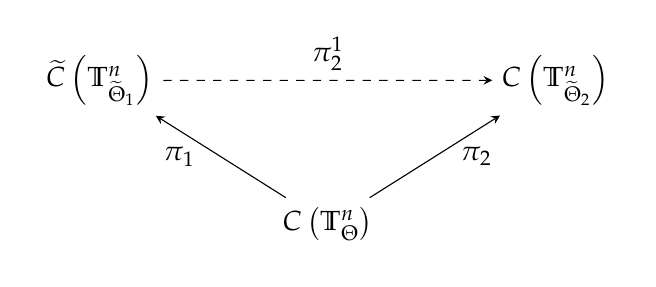
\begin{tikzpicture}
	\matrix (m) [matrix of math nodes,row sep=3em,column sep=4em,minimum width=2em]
	{
		\widetilde  C\left(\mathbb{T}^{n}_{\widetilde{\Th}_1}\right)  &  &  C\left(\mathbb{T}^{n}_{\widetilde{\Th}_2}\right)\\
		&  C\left(\mathbb{T}^{n}_{\Th}\right) & \\};
	\path[-stealth]
	(m-1-1) edge[dashed] node [above] {$\pi^1_2$} (m-1-3)
	(m-2-2) edge node [left]  {$\pi_1~~$} (m-1-1)
	(m-2-2) edge node [right] {$~~\pi_2$} (m-1-3);
	%\draw[dashed,->]   (m-1-1) -- (m-1-3);
	\end{tikzpicture}
	\\
	is commutative then the pair  $\left(\pi_1, \pi_2\right)$ is compliant (cf. Definition \ref{compliant_covering_defn}),
\end{lemma}	
\begin{proof}
	It is proven in   that for the inclusions $\pi_1, \pi_2$ there are  invertible $n \times n$-matrices $M_1$, $M_2$ with integer valued entries such that
	\bean
		\Th \in M_1^{\text{T}} \widetilde{\Th}_1 M_1 + \mathbb{M}_n\left( \Z\right),\\
		\Th \in M_2^{\text{T}} \widetilde{\Th}_2 M_2 + \mathbb{M}_n\left( \Z\right).
	\eean
	If $\pi^1_2$ exists then 
there are lattices $\Ga, \Ga_1\subset \Z^n$ such that
\be\label{nt_lat_eqn}
\begin{split}
	\forall k \in \Z^n\quad \widetilde U_k \in  \pi_2\left(  C\left(\mathbb{T}^{n}_{\widetilde{\Th}_2}\right)\right) \Leftrightarrow k\in \Ga,\\
\forall k \in \Z^n\quad \widetilde U_k \in  \pi^1_2\left(  C\left(\mathbb{T}^{n}_{\widetilde{\Th}_1}\right)\right) \Leftrightarrow k\in \Ga_1.
\end{split}	
\ee	
	Let us check conditions (a)-(d) of the Definition \ref{compliant_covering_defn}.\\
	(a) If there is an injective *-homomorphism $\pi^1_2: C\left(\mathbb{T}^{n}_{\widetilde{\Th}_1}\right) \hookto  C\left(\mathbb{T}^{n}_{\widetilde{\Th}_2}\right)$ then from \cite{schwieger:nt_cov} it follows that there is an invertible $n \times n$-matrices $M$ with integer valued entries such that
	$$
		\Th_1 \in M^{\text{T}} \widetilde{\Th}_2 M + \mathbb{M}_n\left( \Z\right)
	$$
From the Theorem \ref{nt_fin_thm} it follows that $\pi^1_2$  a noncommutative finite-fold  covering (cf. Definition \ref{fin_defn}).\\
(b)  For any $g \in G\left(\left.C\left(\mathbb{T}^{n}_{\widetilde{\Th}_2}\right)~\right|C\left(\mathbb{T}^{n}_{{\Th}}\right) \right)$ from the equations  \eqref{nt_exp_eqn} and \eqref{nt_lat_eqn} it follows that
\bean
k \in \Ga_1 \quad \Leftrightarrow\quad \widetilde U_k \in \pi^1_2\left(  C\left(\mathbb{T}^{n}_{\widetilde{\Th}_1}\right)\right) \text{ AND }  \exists c\in \C \quad g\widetilde U_k=c\widetilde U_k \quad \Rightarrow\\ \Rightarrow g \widetilde U_k \in \pi^1_2\left(  C\left(\mathbb{T}^{n}_{\widetilde{\Th}_1}\right)\right).
\eean
so one has 
$$
G\left(\left.C\left(\mathbb{T}^{n}_{\widetilde{\Th}_2}\right)\right|C\left(\mathbb{T}^{n}_{{\Th}}\right) \right)\pi^1_2\left(  C\left(\mathbb{T}^{n}_{\widetilde{\Th}_1}\right)\right) = \pi^1_2\left(  C\left(\mathbb{T}^{n}_{\widetilde{\Th}_1}\right)\right).
$$
(c)	 From the Theorem \ref{nt_fin_thm} it follows that
\bean
G\left(\left.C\left(\mathbb{T}^{n}_{\widetilde{\Th}_2}\right)\right|C\left(\mathbb{T}^{n}_{{\Th}}\right) \right)\cong \Z^n/\Ga,\\
G\left(\left.C\left(\mathbb{T}^{n}_{\widetilde{\Th}_1}\right)\right|C\left(\mathbb{T}^{n}_{{\Th}}\right) \right) \cong \Z^n/\Ga_1
\eean
where $\Ga_1\subset  \Ga$ the natural homomorphism \\$\phi: G\left(\left.C\left(\mathbb{T}^{n}_{\widetilde{\Th}_2}\right)\right|C\left(\mathbb{T}^{n}_{{\Th}}\right) \right)\to G\left(\left.C\left(\mathbb{T}^{n}_{\widetilde{\Th}_1}\right)\right|C\left(\mathbb{T}^{n}_{{\Th}}\right) \right)$ is equivalent to the homomorphism $\varphi:\Z^n/\Ga\to \Z^n/\Ga_1$. The homomorphism $\varphi$ is surjective, hence $\phi$ is surjective.\\
(d) If $\rho : C\left(\mathbb{T}^{n}_{\widetilde{\Th}_1}\right)\hookto C\left(\mathbb{T}^{n}_{\widetilde{\Th}_2}\right)$ is an injective *-homomorphism such that $\pi_2 = \rho \circ \pi_1$ then both $\pi^1_2$ and $\rho$ can be regarded as *-isomorphisms from $ C\left(\mathbb{T}^{n}_{\widetilde{\Th}_1}\right)$ onto their images. But from \eqref{nt_cov_un_eqn} it follows follows that the image of $\pi^1_2$ coincides with the image of  $\rho$. It follows that there is $g \in \Aut\left(C\left(\mathbb{T}^{n}_{\widetilde{\Th}_1}\right) \right)$ such that 	$\rho =  \pi^1_2 \circ g$. From $\pi_2 = \rho \circ \pi_1$ and $\pi_2 = \pi^1_2 \circ \pi_1$ it follows that $ga = a$ for all $a \in C\left(\mathbb{T}^{n}_{\widetilde{\Th}}\right)$, i.e. $g \in G\left(\left.C\left(\mathbb{T}^{n}_{\widetilde{\Th}_1}\right)\right|C\left(\mathbb{T}^{n}_{{\Th}}\right) \right)$.

\end{proof}

\begin{lemma}\label{nt_diag_lem}
	Let $\pi: C\left(\T^{n}_{{\Th}} \right)\hookto C\left(\T^{n}_{\widetilde{\Th}} \right)$ be an injective *-homomorphism which corresponds to a  noncommutative finite-fold  covering $\left( C\left(\T^{n}_{{\Th}} \right), C\left(\T^{n}_{\widetilde{\Th}} \right), \Z^n / \Ga\right)$. There is a diagonal covering $\left( C\left(\T^{n}_{{\Th}} \right), C\left(\T^{n}_{{\Th/k^2}} \right), \Z^n_k\right)$ and the injective *-homomorphism $\widetilde{\widetilde{\pi}}:C\left(\T^{n}_{\widetilde{\Th}} \right) \to C\left(\T^{n}_{{\Th/m^2}} \right)$ such that following condition hold:
	\begin{itemize}
		\item The homomorphism $\widetilde{\pi}:C\left(\T^{n}_{\widetilde{\Th}} \right)\hookto C\left(\T^{n}_{{\Th/m^2}} \right)$ corresponds an unial noncommutative finite-fold  covering having unique map lifting $\left( C\left(\T^{n}_{\widetilde{\Th}} \right), C\left(\T^{n}_{{\Th/k^2}} \right), \Z^n/ \widetilde{\Ga}\right)$,
		\item Following digram
		\\
		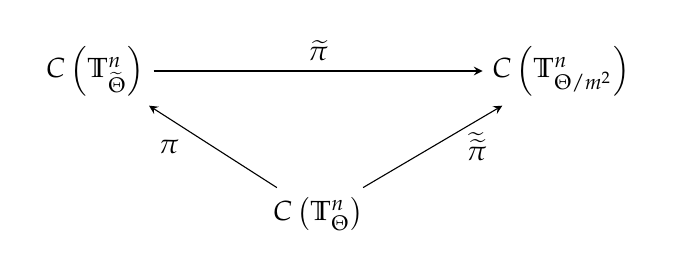
\begin{tikzpicture}
		\matrix (m) [matrix of math nodes,row sep=3em,column sep=4em,minimum width=2em]
		{
			C\left(\T^{n}_{\widetilde{\Th}} \right) & &C\left(\T^{n}_{{\Th/m^2}} \right)\\ 
			& C\left(\T^{n}_{{\Th}}\right)  & \\};
		\path[-stealth]
		(m-1-1) edge node [above] {$\widetilde{\pi}$} (m-1-3)
		(m-2-2) edge node [left]  {$\pi~~~$} (m-1-1)
		(m-2-2) edge node [right] {$~~~\widetilde{\widetilde{\pi}} $} (m-1-3);
		\end{tikzpicture}
		\\
		is commutative. 
		
	\end{itemize}
\end{lemma}
\begin{proof}
	From the construction \ref{nt_ff_inclusion_empt} it turns out that:
	\bean
	\Ga = M\Z^n,\\
	\Th = M^{\mathrm{T}} \widetilde{\Th} M + P\\
	\widetilde{\Th} = \left( M^{\mathrm{T}}\right)^{-1}  {\Th} M^{-1}+ \left( M^{\mathrm{T}}\right)^{-1}  P M^{-1}
	\eean
	where $P \in \mathbb{M}_n\left( \Z\right)$. There is $m \in \N$ such that $N = mM^{-1} \in \mathbb{M}_n\left( \Z\right)$, or equivalently 
	$$
	MN = \begin{pmatrix}
	m& \ldots & 0  \\
	\vdots &\ddots  & \vdots \\
	0 &\ldots & m  \\
	\end{pmatrix}.
	$$
	If
	$$
	\widetilde{\widetilde{ \Th}}= \frac{\widetilde{\Th}-\left( M^{\mathrm{T}}\right)^{-1}  P M^{-1} }{m^2}
	$$
	then
	\bean
	\Th = mM^{\mathrm{T}} \widetilde{\widetilde{ \Th}} Mm,\\
	\widetilde{ \Th} = m 	\widetilde{\widetilde{ \Th}}m-  m\left( M^{\mathrm{T}}\right)^{-1}  P M^{-1}m =\\=m 	\widetilde{\widetilde{ \Th}}m-  N^{\mathrm{T}} P N \in m 	\widetilde{\widetilde{ \Th}}m + \mathbb{M}_n\left( \Z\right).
	\eean
	So there are noncommutative finite-fold coverings $\pi': C\left( \T^n_{{\Th}}\right) \hookto C\left( \T^n_{\widetilde{\widetilde{ \Th}}}\right)$, $\pi'':C\left( \T^n_{\widetilde{\Th}}\right) \hookto C\left( \T^n_{\widetilde{\widetilde{ \Th}}}\right)$, which correspond to triples $\left( C\left( \T^n_{{\Th}}\right), C\left( \T^n_{\widetilde{\widetilde{ \Th}}}\right), \Z^n / mM\Z^n\right)$, $\left(C\left( \T^n_{\widetilde{\Th}}\right), C\left( \T^n_{\widetilde{\widetilde{ \Th}}}\right), \Z^n_m \right)$  
	From $N = mM^{-1}$ it turns out
	\bean
	\Th= m M^{\mathrm{T}} N^{\mathrm{T}}\left( N^{\mathrm{T}}\right)^{-1}  \widetilde{\widetilde{ \Th}}  P N^{-1}NMm= m^2\left(  \left( N^{\mathrm{T}}\right)^{-1}  \widetilde{\widetilde{ \Th}}   N^{-1}\right)  m^2,\\
	\left( N^{\mathrm{T}}\right)^{-1}  \widetilde{\widetilde{ \Th}}   N^{-1} = \frac{\Th}{m^{4}},\\
	\widetilde{\widetilde{ \Th}} = N^{\mathrm{T}}\left( N^{\mathrm{T}}\right)^{-1}  \widetilde{\widetilde{ \Th}}  P N^{-1}N = N^{\mathrm{T}} \frac{\Th}{m^{4}}N
	\eean 
	From the above equations it follows that there is  a noncommutative finite-fold covering ${\widetilde{\pi}}:C\left( \T^n_{\widetilde{\widetilde{\Th}}}\right) \hookto C\left( \T^n_{\Th/m^4}\right)$ which corresponds to the triple $$\left( C\left( \T^n_{\widetilde{\widetilde{\Th}}}\right), C\left( \T^n_{\Th/m^4}\right), \Z^n/N\Z^n\right).$$ The composition $\widetilde{\widetilde{\pi}} = {\widetilde{\pi}}\circ \pi: C\left( \T^n_{\Th}\right) \to C\left( \T^n_{\Th/m^4}\right)$ corresponds to the diagonal covering $\left(C\left( \T^n_{\Th}\right), C\left( \T^n_{\Th/m^4}\right), \Z^n_{m^2} \right)$. 
\end{proof}
\begin{corollary}\label{nt_cofinal_cor}
	If $\mathfrak{S}_{C\left( \T^n_{\Th}\right)}$ is a family of all noncommutative finite-fold coverings given by the Theorem \ref{nt_fin_thm} then following conditions hold:
	\begin{enumerate}
		\item[(i)] Let $\left\{p_k\right\}_{k \in \N}\in \N$ is a sequence such that for every $s \in \N$ there are $j, m \in \N$ which satisfy to the following condition 
		\bean
		sm = \prod_{k = 1}^j p_j.
		\eean
		If $m_j = \prod_{k = 1}^j p_k$ then the ordered set 
		$$
		\mathfrak{S}_{C\left(\T^{n}_{{\Th}} \right)}^\N=\left\{ \left( C\left(\T^{n}_{{\Th}} \right), C\left(\T^{n}_{\Th/m_j^2} \right), \Z^n_{m_j}\right)  \right\}_{j \in \N}
		$$ 
		is a cofinal subset (cf. Definition \ref{cofinal_defn}) of $\mathfrak{S}_{C\left(\T^{n}_{{\Th}} \right)}$. 
		\item[(ii)] The family $\mathfrak{S}_{C\left( \T^n_{\Th}\right)}$ is a directed set with respect to the given by \eqref{fg_ord_eqn} order.
	\end{enumerate}
	
\end{corollary}

\begin{proof}
(i) Let $\left( C\left(\T^{n}_{{\Th}} \right), C\left(\T^{n}_{\widetilde{\Th}} \right), \Z^n / \Ga\right)$ be a noncommutative finite-fold  covering  having unique path  lifting. From the  Lemma \ref{nt_diag_lem} it turns out that there is a noncommutative finite-fold  covering $C\left(\T^{n}_{\widetilde{\Th}} \right) \hookto C\left(\T^{n}_{{\Th}/s^2}\right)$. Otherwise there is $j \in \N$ such $m_j = sm$, so there are following noncommutative finite-fold  coverings
	\be\label{nt_cof_eqn}
	\begin{split}
		C\left(\T^{n}_{{\Th}/s^2}\right) \hookto C\left(\T^{n}_{{\Th}/m_j^2}\right),\\
		C\left(\T^{n}_{\widetilde{\Th}}\right) \hookto C\left(\T^{n}_{{\Th}/m_j^2}\right).
	\end{split}
	\ee
	From \eqref{nt_cof_eqn} it turns out that
	$$
	\left( C\left(\T^{n}_{{\Th}} \right)\to C\left(\T^{n}_{{\Th}/m_j^2} \right)\right) \ge \left( C\left(\T^{n}_{{\Th}} \right)\to C\left(\T^{n}_{\widetilde{\Th}} \right)\right),
	$$
	i.e. $\left\{ \left( C\left(\T^{n}_{{\Th}} \right), C\left(\T^{n}_{\Th/m_j^2} \right), \Z^n_{m_j}\right)  \right\}_{j \in \N}$ is cofinal.\\
	(ii) Follows from (i).
\end{proof}





%\begin{lemma}
%	In the above situation the  unital noncommutative finite-fold  covering $$\left( C\left(\T^{n}_{{\Th}} \right), C\left(\T^{n}_{\widetilde{\Th}} \right), \Z^n / \Ga\right)$$ have a unique map lifting (cf. Definition \ref{upl_defn}). 
%\end{lemma}
%\begin{proof}
%	The linear span of the generators $\left\{\widetilde{U}_x\right\}\in M^{-1}\Z^n$ is dense in $C\left(\T^{n}_{\widetilde{\Th}} \right)$. For any $x \in M^{-1}\Z^n$ there is $m_x \in \N$ such that $m_xx \in \Z^n$, it follows that $\widetilde{U}_x^{m_x} = u_x \in C\left(\T^{n}_{{\Th}}\right) $. Moreover $u_x$ is unitary, so there is a Borel-measured $\varphi_x$ such that $\widetilde{U}_x = \varphi\left(u_x \right)$. From the Corollary \ref{borel_path_lift_cor} it turns out that $\left( C\left(\T^{n}_{{\Th}} \right), C\left(\T^{n}_{\widetilde{\Th}} \right), \Z^n / \Ga\right)$ has the {unique path lifting}
%\end{proof}

\subsection{Induced representation}\label{nt_i_sec}
\paragraph*{}

Let us consider an unital noncommutative finite-fold  covering $$\left( C\left(\T^{n}_{{\Th}} \right), C\left(\T^{n}_{\widetilde{\Th}} \right), \Z^n / \Ga, \pi\right)$$ given by the Theorem \ref{nt_fin_thm}. The group	$\Z^n/\Ga$ is and commutative group, hence any irreducible representation of $\Z^n/\Ga$ has dimension 1. From the proof of the Lemma \ref{nt_fin_cov_gr_lem} it follows that the moduli space of the irreducible representations $\Z^n / \Ga$ coincides with $\Ga^\vee/ \Z^n $ and any irreducible representation corresponds to a character the given by \eqref{nt_char_r_eqn} character $\chi_{\overline{x}}: \Z^n / \Ga \to \C$. It is known the orthogonality of characters (cf. \cite{hamermesh:group}), i.e.
\be\label{nt_ort_eqn}
\sum_{g \in \Z^n / \Ga} \overline{\chi}_{\overline x_1}\left( g\right) \chi_{\overline x_1}\left( g\right)= \left\{\begin{array}{c l}
	\left|\Z^n / \Ga\right|   & \overline x_1 = \overline x_2 \\
	0 & \overline x_1 \neq\overline x_2 .
\end{array}\right.
\ee

Otherwise one has
\bean
%\chi_{\overline {x + l}}= \chi_{\overline {x}}; \quad \forall l \in \Z^n,\\
g \widetilde{U}_k = \chi_{\overline {M^{-1}k}}\left(g \right)  \widetilde{U}_k;\quad \forall g \in \Z^n / \Ga
\eean
and taking into account \eqref{nt_ort_eqn} following condition holds
\be\label{nt_hprod_eqn}
\begin{split}
	\left\langle \widetilde{U}_{k_1 }, \widetilde{U}_{k_2} \right\rangle_{C\left(\mathbb{T}^n_{{\Th}}\right)} = \sum_{g \in \Z^n / \Ga } g\left( \widetilde{U}^*_{k_1 }\widetilde{U}_{k_2 }\right)=
	\\
	 =\sum_{g \in \Z^n / \Ga }\overline{\chi}_{\overline {M^{-1}k_1}}\left( g\right) \chi_{\overline {M^{-1}k_2}}\left( g\right)\widetilde{U}^*_{k_1 }\widetilde{U}_{k_2 }
	= \\
	 =\sum_{g \in \Z^n / \Ga }\overline{\chi}_{\overline {M^{-1}k_1}}\left( g\right) \chi_{\overline {M^{-1}k_2}}\left( g\right)|e^{-\pi ik_1 ~\cdot~ \widetilde\Theta k_2}\widetilde{U}_{k_2-k_1 }
= \\
	= \left\{\begin{array}{c l}
		\left|\Z^n / \Ga\right|e^{-\pi ik_1 ~\cdot~ \widetilde\Theta k_2} U_{M^{-1}\left(k_2 - k_1 \right) } \in C\left(\T^{n}_{{\Th}} \right)  & k_1 - k_2 \in \Ga \\
		0 & k_1 - k_2 \notin \Ga .
	\end{array}\right.
\end{split}
\ee
From the equation \eqref{nt_l2_eqn} it follows that
\be\label{nt_huprod_eqn}
\begin{split}
U_{M^{-1}\left(k_2 - k_1 \right)}\xi_l = e^{-\pi iM^{-1}\left(k_2 - k_1 \right) ~\cdot~ \Theta l}\xi_{M^{-1}\left(k_2 - k_1 \right) + l}= 
\\
=e^{-\pi i\left(k_2 - k_1 \right) ~\cdot~ \widetilde\Theta Ml}\xi_{M^{-1}\left(k_2 - k_1 \right) + l}
\end{split}
\ee
Let $\rho: C\left(\mathbb{T}^n_{{\Th}}\right) \to B\left( L^2\left(C\left(\mathbb{T}^n_{\Theta}\right), \tau\right)\right)$ be the described in \ref{nt_gns_empt} faithful GNS-representation.
If $\widetilde \rho: C\left(\T^{n}_{\widetilde{\Th}} \right) \to B\left(\widetilde \H \right)$ is the induced by the pair 
$$
\left(\rho, \left( C\left(\T^{n}_{{\Th}} \right), C\left(\T^{n}_{\widetilde{\Th}} \right), \Z^n / \Ga, \pi\right)\right)
$$
representation (cf. Definition \ref{induced_repr_defn}) then $\widetilde \H$ is the Hilbert norm completion of the tensor product $C\left(\T^{n}_{\widetilde{\Th}} \right) \otimes_{C\left(\T^{n}_{{\Th}} \right)} L^2\left(C\left(\mathbb{T}^n_{\Theta}\right), \tau\right)$. Denote by $\left(\cdot, \cdot \right)_{\widetilde \H}$ the scalar product on $\widetilde \H$ given by \eqref{induced_prod_equ}.
If $\xi_{l_1}, \xi_{l_2} \in L^2\left(C\left(\mathbb{T}^n_{\Theta}\right), \tau\right)$ then from \eqref{nt_hprod_eqn}, \eqref{nt_huprod_eqn} and \eqref{nt_xi_eqn} it follows that
\be\label{nt_hh_product_eqn}
\begin{split}
\left(\widetilde{U}_{k_1 } \otimes \xi_{l_1} , \widetilde{U}_{k_2 } \otimes \xi_{l_2} \right)_{\widetilde \H} =
\\
=\left\{\begin{array}{c l}
	e^{-\pi ik_1 ~\cdot~ \widetilde\Theta k_2}e^{\pi i\left(k_2 - k_1 \right) ~\cdot~ \widetilde\Theta Ml_2}	\left|\Z^n / \Ga\right|  & k_1 + Ml_1 = k_2 + Ml_2  \\
	0 & k_1 + Ml_1 \neq k_2 + Ml_2 .
\end{array}\right.
\end{split}
\ee
From the Equation \eqref{nt_hh_product_eqn} it turns out that $\widetilde \H$ is a Hilbert direct sum 
$$
\widetilde\H = \bigoplus_{p \in \Z^n} \widetilde\H_p
$$
of one-dimensional Hilbert spaces such that
$$
\widetilde{U}_{k } \otimes \xi_{l}\in \widetilde\H_{k + Ml}
$$
If $k_1 + Ml_1 = k_2 + Ml_2$  and
\bean
\widetilde\xi_1 \bydef \sqrt{\left|\Z^n / \Ga\right|} e^{-\pi ik_1 ~\cdot~ \widetilde\Theta Ml_1}\widetilde{U}_{k_1 } \otimes \xi_{l_1},\\ 
\widetilde\xi_2 \bydef \sqrt{\left|\Z^n / \Ga\right|} e^{-\pi ik_2 ~\cdot~ \widetilde\Theta Ml_2}\widetilde{U}_{k_2 } \otimes \xi_{l_2}
\eean
then from \eqref{nt_hh_product_eqn} it follows that 
\bean
\begin{split}
\left(\widetilde \xi_{1} ,\widetilde  \xi_{2} \right)_{\widetilde \H}= 	e^{-\pi ik_1 ~\cdot~ \widetilde\Theta k_2}e^{\pi i\left(k_2 - k_1 \right) ~\cdot~ \widetilde\Theta Ml_2}e^{\pi ik_1 ~\cdot~ \widetilde\Theta Ml_1} e^{-\pi ik_2 ~\cdot~ \widetilde\Theta Ml_2}=e^{\pi ix},\\
\text{where } x = - k_1 \cdot \widetilde\Theta k_2 + \left(k_2 - k_1 \right) \cdot \widetilde\Theta Ml_2+ k_1 \cdot \widetilde\Theta Ml_1- k_2 ~\cdot~ \widetilde\Theta Ml_2=
\\
= - k_1 \cdot \widetilde\Theta k_2 +k_1\cdot \left(Ml_2 - Ml_1 \right)=  -k_1 \cdot \widetilde\Theta k_2  + k_1 \cdot \widetilde\Theta\left(k_2 - k_1 \right) 
\end{split}
\eean
Since $\widetilde\Theta$ is skew symmetric one has $x = 0$ it follows that $\left(\widetilde \xi_{1} ,\widetilde  \xi_{2} \right)_{\widetilde \H}=1$ and taking into account $\left\| \widetilde \xi_1\right\|_{\widetilde\H}=\left\| \widetilde \xi_2\right\|_{\widetilde\H}=1$ one has $\widetilde\xi_1 = \widetilde\xi_2$. So there is the orthonormal basis $\left\{\widetilde\xi_p\right\}_{p \in \Z^n}$ such that
\be\label{nt_basis_eqn}
\widetilde\xi_{p} \bydef \sqrt{\left|\Z^n / \Ga\right|} e^{-\pi ik ~\cdot~ \widetilde\Theta Ml}\widetilde{U}_{k} \otimes \xi_{l}\text{ where } p = Ml + k.
\ee
and for all $p\in \Z^n$ the element  $\widetilde\xi_{p}$ does not depend on the representation $p = Ml + k$. Direct check shows that
\be\label{nt_basis_act_eqn}
\widetilde U_k \widetilde\xi_{l} = 	e^{\pi ik ~\cdot~ \widetilde\Theta l}\widetilde\xi_{Mk + l}.
\ee
Using equations  \eqref{nt_basis_eqn} and \eqref{nt_l2_eqn} one has the following lemma.


\begin{lemma}
	If	$\widetilde \rho: C\left(\T^{n}_{\widetilde{\Th}} \right) \to B\left(\widetilde \H \right)$ is the induced by the pair 
	$$
	\left(\rho, \left( C\left(\T^{n}_{{\Th}} \right), C\left(\T^{n}_{\widetilde{\Th}} \right), \Z^n / \Ga, \pi\right)\right)
	$$ then $\widetilde \rho$ is equivalent to the described  \ref{nt_gns_empt} faithful GNS representation.
\end{lemma}


   \subsection{Coverings of spectral triples}\label{nt_triple_fin_cov}



\begin{lemma}\label{nt_smooth_matr_lem}
Let $\left( C\left(\T^{n}_{{\Th}} \right), C\left(\T^{n}_{\widetilde{\Th}} \right), \Z^n / \Ga, \pi\right)$ be an unital noncommutative finite-fold  covering given by the Theorem \ref{nt_fin_thm}. Let $\left\lbrace \widetilde x_1,\dots, \widetilde x_N\right\rbrace  \subset  \Z^n$ is a set of representatives of  $\Z^n / \Ga$.
	\begin{itemize}
		\item [(i)] The finite family $\left\{\widetilde U_{\widetilde x_j}\right\}_{j= 1, ..., N}\subset \Coo\left(\T^n_{\widetilde\Th }\right) $  satisfies to the Lemma \ref{smooth_matr_lem}.
		\item[(ii)] 
		\be\label{nt_smooth_lcond_eqn}
		C\left(\T^n_{\widetilde\Th }\right)  \cap \mathbb{M}_{N}\left(\Coo\left(\T^n_{\Th }\right)\right) = \Coo\left(\widetilde M \right).
		\ee
		\item[(iii)] The  given by the Theorem  \ref{nt_fin_thm} unital noncommutative finite-fold covering \\$\left( C\left(\T^{n}_{{\Th}} \right), C\left(\T^{n}_{\widetilde{\Th}} \right), \Z^n / \Ga, \pi\right)$  is smoothly invariant (cf. Definition \ref{smooth_defn}).
	\end{itemize}
\end{lemma}
\begin{proof}
	(i)
Let us prove that $\left\{\widetilde U_{\widetilde x_j}\right\}$ satisfies to conditions (a) and (b) of the Lemma \ref{smooth_matr_lem}.
	\begin{enumerate}
		\item [(a)] Follows from 	
		$$
		\left\langle \widetilde U_{\widetilde x_j},  \widetilde U_{\widetilde x_k}\right\rangle = \begin{cases}
		e^{\pi i x_j \widetilde \Th x_k}U_{M^{-1}\left(x_k - x_j \right) }\in \Coo\left(\T^{n}_{{\Th}} \right) & x_j - x_k\in \Ga\\
		0 & x_j\neq x_k
		\end{cases}
		$$
		\item[(b)] 	For any $j = 1,..., n$ and $g \in \Z^n / \Ga$ one has $g \widetilde U_{\widetilde x_j} =  \widetilde U_{\widetilde x_j}  \left( \chi_{\overline{M^{-1}\widetilde x_j}}\left(g \right) \cdot 1_{\Coo\left(\T^n_{\Th }\right)} \right) $.
	\end{enumerate}
(ii) For any $\widetilde a \in C\left(\T^{n}_{\widetilde{\Th}} \right)$ from the Theorem \ref{nt_fin_thm} it follows that 
		\be\label{nt_al_eqn}
		\widetilde a = \sum_{l = 1}^N a_l \widetilde U_{\widetilde x_l} \text{ where } a_l\in C\left(\T^{n}_{{\Th}} \right) 
		\ee
		On the other hand one has
		\bean
		\left\langle \widetilde U_{\widetilde x_j},  \widetilde a \widetilde U_{\widetilde x_k}\right\rangle = \sum_{g \in \Z^n / \Ga} g\left( \widetilde U^*_{x_j}\widetilde a \widetilde U_{\widetilde x_k}\right)= \sum_{g \in \Z^n / \Ga} \sum_{l=1}^N g \left(\widetilde U_{\widetilde x_j}a_l \widetilde U_{\widetilde x_l}\widetilde U_{\widetilde x_k} \right) =\\
		= \sum_{g \in \Z^n / \Ga} \sum_{l=1}^N\chi_{\overline{M^{-1}\left( \widetilde x_l + \widetilde x_k - \widetilde x_j\right) }} g   \left(\widetilde U_{\widetilde x_j}a_l \widetilde U_{\widetilde x_l}\widetilde U_{\widetilde x_k} \right)
		\eean 
		where $\overline {M^{-1}\left( \widetilde x_l + \widetilde x_k - \widetilde x_j\right) }\in \Ga^\vee/\Z^n$ (cf. \eqref{nt_dual_eqn}) represented by $M^{-1}\left( \widetilde x_l + \widetilde x_k - \widetilde x_j\right)\in \Q^n $ and $\chi_{\overline{M^{-1}\left( \widetilde x_l + \widetilde x_k - \widetilde x_j\right) }}$ is a character which corresponds to $\chi_{\overline{M^{-1}\left( \widetilde x_l + \widetilde x_k - \widetilde x_j\right) }}$. Since the set $\left\lbrace \widetilde x_1,\dots, \widetilde x_N\right\rbrace  \subset  \Z^n$ is a set of representatives of  $\Z^n / \Ga$
		one has
		$$
		\overline{M^{-1}\left( \widetilde x_l + \widetilde x_k - \widetilde x_j\right) }= 0\quad \Leftrightarrow \quad M^{-1}\left( \widetilde x_l + \widetilde x_k - \widetilde x_j\right)= 0.
		$$
		Otherwise it is known that
		$$
		\sum_{g \in \Z^n / \Ga} \chi_{\overline{M^{-1}\left( \widetilde x_l + \widetilde x_k - \widetilde x_j\right) }}\left( g\right) = \begin{cases}
		N & \overline{M^{-1}\left( \widetilde x_l + \widetilde x_k - \widetilde x_j\right) }= 0
		\\
		0 & \overline{M^{-1}\left( \widetilde x_l + \widetilde x_k - \widetilde x_j\right) }\neq  0
		\end{cases}
		$$
		If $ \widetilde x_l + \widetilde x_k - \widetilde x_j=0$ and $a_l = \sum_{p \in \Z^n}c^l_k U_k$ where $c^l_k\in \C$ and $a'_l =\widetilde U_{\widetilde x_j}a_l \widetilde U_{\widetilde x_l}\widetilde U_{\widetilde x_k}= \sum_{p \in \Z^n}c'^l_k U_k$ then from \eqref{nt_unitary_product_comm_eqn} it follows that $\left|c'^l_k \right| = \left|c^l_k \right|$ for all $k \in \Z$. Hence
		$$
		\mathrm{sup}_{k \in \mathbb{Z}^n}\left(1 + \|k\|\right)^s \left|c^l_k\right| = \mathrm{sup}_{k \in \mathbb{Z}^n}\left(1 + \|k\|\right)^s \left|c'^l_k\right|
		$$
		and taking into account \eqref{schwartz_z_eqn} one has
		$$
		a_l = \sum_{p \in \Z^n}c^l_k U_k  \in \Coo\left(\T^n_\Th \right)\quad \Leftrightarrow\quad a'_l=\widetilde U_{\widetilde x_j}a_l \widetilde U_{\widetilde x_l}\widetilde U_{\widetilde x_k}=\sum_{p \in \Z^n}c'^l_k U_k\in \Coo\left(\T^n_\Th \right).
		$$
So from \eqref{nt_al_eqn} it turns out
$$
\forall l = 1,..., n\quad a'_l \in \Coo\left(\T^n_\Th \right) \quad \Rightarrow \quad \widetilde a\in \Coo\left(\T^n_{\widetilde\Th} \right),
$$
or, equivalently
$$
\forall j, k  = 1,..., n\quad\left\langle \widetilde U_{\widetilde x_j},  \widetilde a \widetilde U_{\widetilde x_k}\right\rangle\in \Coo\left(\T^n_\Th \right) \quad \Rightarrow \quad \widetilde a \in \Coo\left(\T^n_{\widetilde\Th} \right).
$$
\\
Conversely if there are $j, k \in 1,..., n$ such that $\left\langle \widetilde U_{\widetilde x_j},  \widetilde a \widetilde U_{\widetilde x_k}\right\rangle\notin \Coo\left(\T^n_\Th \right)$ and $\widetilde x_l = \widetilde x_k - \widetilde x_j$ then $a_l \notin \Coo\left(\T^n_\Th \right)$. If $a_l =  \sum_{k \in \Z^n} c_k U_k$ and $\widetilde a =  \sum_{\widetilde k \in \Z^n} \widetilde c_{\widetilde k} \widetilde U_{\widetilde k}$ then from \eqref{nt_al_eqn} it follows that
$$
 \left|\widetilde c_{M k + \widetilde x_l } \right| =  \left|c_k  \right| 
$$
There is $c \in \R$ such that $c > 4$ and
$$
\left\|k\right\|> c \quad \Rightarrow \quad\left\|M k + \widetilde x_l\right\|> \frac{\left\|k\right\|}{2} \quad \Rightarrow \quad \left(1 + \|M k + \widetilde x_l\|\right)^2 > 1 + \|k\|.
$$
From $a_l \notin \Coo\left(\T^n_\Th \right)$
and \eqref{schwartz_z_eqn} it follows that there is $s \in \N$ such that
$$
\sup_{k \in \mathbb{Z}^n}\left(1 + \|k\|\right)^s \left|c_k\right|= \infty.
$$
If $C > 0$ is a big number then there is $k \in \Z^2$ such that  $\left\|k\right\|> c$ and $\left(1 + \|k\|\right)^s \left|c_k\right| > C$. It follows that
$$
\left(1 + \|M k + \widetilde x_l\|\right)^{2s} > C.
$$
So 
$$
\sup_{\widetilde k \in \mathbb{Z}^n}\left(1 + \|\widetilde k\|\right)^{2s} \left|\widetilde c_{\widetilde k}\right|= \infty
$$
and from \eqref{schwartz_z_eqn} it follows that $\widetilde a \notin  \Coo\left(\T^n_{\widetilde\Th} \right)$.
In result 
$$
\Coo\left(\T^n_{\widetilde\Th} \right) = \left\{\left.\widetilde a \in  \Coo\left(\T^n_{\widetilde\Th} \right)\right| \left\langle \widetilde U_{\widetilde x_j},  \widetilde a \widetilde U_{\widetilde x_k}\right\rangle \in \Coo\left(\T^n_{\Th} \right)\quad j, k \in 1,..., n\right\}.
$$
The Equation \eqref{nt_al_eqn} follows from (i) of the Lemma \ref{smooth_matr_lem}.\\
(iii) Follows from  (ii) of the  Lemma \ref{smooth_matr_lem}. 
\end{proof}

\paragraph*{}
The Hilbert space of relevant to spectral triple is $\widetilde{\H}^m= \widetilde{\H}\otimes \C^m$ where $m=2^{[n/2]}$ and $\widetilde{\H}$ is described in \ref{nt_i_sec} and the action of $C\left(\mathbb{T}^n_{\widetilde{\Th}} \right)$ on $\widetilde{\H}$ is given by \eqref{nt_l2_eqn}. The action of $C\left(\mathbb{T}^n_{\widetilde{\Th}} \right)$ on  $\widetilde{\H}^m$ is diagonal. Let $\Om^1_D$ is the {module of differential forms associated} with the spectral triple  $\left( \A, \H, D\right)$ (cf. Definition \ref{ass_cycle_defn}). We suppose that $\Ga = M\Z^n$ where $M \in \mathbb{M}_n\left(\Z\right)$ is a diagonal matrix
$$
M = \begin{pmatrix} k_1  & \dots & 0 \\
\vdots  & \ddots & \vdots \\
0  & \dots & k_n 
\end{pmatrix}\quad k_1,..., k_n \in \N
$$ 
Let us consider a map
\bean
\widetilde\nabla : \Coo\left(\mathbb{T}^n_{\widetilde{\Th}} \right) \to \Coo\left(\mathbb{T}^n_{\widetilde{\Th}} \right) \otimes_{\Coo\left(\mathbb{T}^n_{{\Th}} \right)} \Om^1_D,\\
\widetilde{a} \mapsto \sum_{\mu = 1}^n \frac{\partial a}{\partial x_\mu} \otimes u^*_\mu \left[ D, u_\mu \right]= \sum_{\mu = 1}^n \frac{\partial a}{\partial x_\mu} \otimes \ga^\mu
\eean
where $\ga^\mu$ Clifford (Gamma) matrices in $\mathbb{M}_n(\mathbb{C})$ satisfying the relation
\eqref{nt_gam_eqn}

The map satisfies  to the following equation
\be\label{nt_nabla_u_eqn}
\nabla \widetilde{ U}_{\widetilde{l} = \left(\widetilde{l}_1, \dots, \widetilde{l}_n \right) } = \sum_{\mu = 1}^n\frac{\widetilde{l}_\mu}{k_\mu} \widetilde{ \mathcal U}_{\widetilde{l}} \otimes \ga^\mu.
\ee
If  $U_{l = \left(l_1,\dots,l_n \right) }\in \Coo\left(\mathbb{T}^n_{{\Th}} \right)$, $\widetilde{l}'=\left( l_1k_1,\dots, l_nk_n\right)$, $\widetilde{l}'' = \widetilde{l} + \widetilde{l}'$ then  from \eqref{nt_unitary_product_eqn} % and \eqref{nt_cov_eqn} 
it turns out
\bean
\widetilde{  U}_{\widetilde{l}} U_l e^{-\pi i\widetilde{l} ~\cdot~ \widetilde{\Theta} \widetilde{l}'} U_{\widetilde{l}''=\widetilde{l} + \widetilde{l}'}
\eean
and taking into account \eqref{nt_nabla_u_eqn} one has
\bean
\nabla \left( \widetilde{  U}_{\widetilde{l}} U_l\right) = e^{-\pi i\widetilde{l} ~\cdot~ \widetilde{\Theta} \widetilde{l}'}\sum_{\mu = 1}^n\frac{l_\mu k_\mu+\widetilde{l}_\mu}{k_\mu} \widetilde{ \mathcal U}_{\widetilde{l}''} \otimes \ga^\mu= \\=e^{-\pi i\widetilde{l} ~\cdot~ \widetilde{\Theta} \widetilde{l}'}\sum_{\mu = 1}^n\frac{\widetilde{l}_\mu}{k_\mu} \widetilde{ \mathcal U}_{\widetilde{l}''} \otimes \ga^\mu + e^{-\pi i\widetilde{l} ~\cdot~ \widetilde{\Theta} \widetilde{l}'}\sum_{\mu = 1}^nl_\mu \widetilde{ \mathcal U}_{\widetilde{l}''} \otimes \ga^\mu=\\= \sum_{\mu = 1}^n\frac{\widetilde{l}_\mu}{k_\mu} \widetilde{  U}_{\widetilde{l}} U_l \otimes \ga^\mu + \sum_{\mu = 1}^nl_\mu \widetilde{  U}_{\widetilde{l}} U_l \otimes \ga^\mu =\\= \sum_{\mu = 1}^n\frac{\widetilde{l}_\mu}{k_\mu}\left(  \widetilde{  U}_{\widetilde{l}} \otimes \ga^\mu\right)  U_l +  \widetilde{  U}_{\widetilde{l}} \otimes \sum_{\mu = 1}^nl_\mu U_l \otimes \ga^\mu =\\=
\left(\nabla\widetilde{  U}_{\widetilde{l}} \right) U_l + \widetilde{  U}_{\widetilde{l}} \otimes \left[D, U_l \right] = \left(\nabla\widetilde{  U}_{\widetilde{l}} \right) U_l + \widetilde{  U}_{\widetilde{l}} \otimes d U_l.
\eean
where $d U_l$ is given by  \eqref{diff_map_eqn}. Right part of the above equation is a specific case of \eqref{conn_defn}, i.e. elements $\widetilde{  U}_{\widetilde{l}}$ satisfy condition $\eqref{conn_defn}$. Since $\C$-linear span of $\left\{\widetilde{  U}_{\widetilde{l}}\right\} $ (resp. $\left\{{  U}_{{l}}\right\}$ ) is dense in $\Coo\left(\mathbb{T}^n_{\widetilde{\Th}} \right)$ (resp. $\Coo\left(\mathbb{T}^n_{{\Th}} \right)$) the map $\nabla$ is a connection. If $\left( \overline{p}_1, \dots,\overline{p}_n\right) \in \Z_{k_1}\times \dots \times \Z_{k_1}$ then from
$$
\left( \overline{p}_1, \dots,\overline{p}_n\right) \widetilde{ U}_{\widetilde{l}} = e^{2\pi i \frac{p_1l_1}{k_1} }\cdot \dots\cdot  e^{2\pi i \frac{p_nl_n}{k_n} } \widetilde{ U}_{\widetilde{l}}
$$
it turns out 
\bean
\nabla\left( \left( \overline{p}_1, \dots,\overline{p}_n\right) \widetilde{ U}_{\widetilde{l}}\right)  = e^{2\pi i \frac{p_1l_1}{k_1} }\cdot ...\cdot  e^{2\pi i \frac{p_nl_n}{k_n} } \sum_{\mu = 1}^n\frac{\widetilde{l}_\mu}{k_\mu} \widetilde{ \mathcal U}_{\widetilde{l}} \otimes \ga^\mu=\left( \overline{p}_1, \dots,\overline{p}_n\right)\left( \nabla \widetilde{ U}_{\widetilde{l}}\right), 
\eean
i.e. $\nabla$ is $\Z_{k_1}\times \dots \times \Z_{k_1}$-equivariant, i.e it satisfies to \eqref{equiv_conn_eqn}. 
If $\widetilde{\xi}_l = \Psi_{\widetilde{ \Th}}\left( \widetilde{U}_{\widetilde{l}}\right)=  \widetilde{U}_l \otimes 1_{C\left(\mathbb{T}^n_{\Th}\right)}$ then from $\left[D,  1_{C\left(\mathbb{T}^n_{\Th}\right)} \right] = 0$ it turns out that given by \eqref{d_defn_eqn} Dirac operator satisfy to following condition
\bean
\widetilde{D} \left( \widetilde{\xi}_{\widetilde{l}} \otimes x\right) = \nabla\left(\widetilde{U}_{\widetilde{l}} \right) \left( 1_{C\left(\mathbb{T}^n_{\Th}\right)} \otimes x\right) + \widetilde{U}_{\widetilde{l}} D\left(   1_{C\left(\mathbb{T}^n_{\Th}\right)} \otimes x\right)= \\= \sum_{\mu = 1}^n\frac{\widetilde{l}_\mu}{k_\mu} \widetilde{ \xi}_{\widetilde{l}} \otimes \ga^\mu x_\mu ; ~~\forall x =\begin{pmatrix} x_1 \\\dots\\ x_m \end{pmatrix} \in \C^m. 
\eean




\paragraph*{} Let us consider following objects
\begin{itemize}
	\item The spectral triple $\left( C^{\infty}(\mathbb{T}^n_{\Theta}),L^2\left(C\left(\mathbb{T}^n_{\Theta}\right), \tau\right)\otimes\mathbb{C}^{m},D\right) $ given by \eqref{nt_sp_tr_eqn},
	\item An unital noncommutative finite-fold  covering $\left(C\left(\mathbb{T}^n_{\Th}\right), C\left(\mathbb{T}^n_{\widetilde{\Th}}\right),\mathbb{Z}_{k_1}\times...\times\mathbb{Z}_{k_n}\right)$ given by the Theorem \ref{nt_fin_thm}.
\end{itemize}

Summarize above constructions one has the following theorem.

\begin{thm}\label{nt_st_fin_cov_thm}
	The $\left(C\left(\mathbb{T}^n_{\Th}\right), C\left(\mathbb{T}^n_{\widetilde{\Th}}\right),\mathbb{Z}_{k_1}\times...\times\mathbb{Z}_{k_n}\right)$-lift of the spectral triple $$\left( C^{\infty}(\mathbb{T}^n_{\Theta}),L^2\left(C\left(\mathbb{T}^n_{\Theta}\right), \tau\right)\otimes\mathbb{C}^{m},D\right) $$ is the spectral  triple $\left(\Coo\left(\mathbb{T}^n_{\widetilde{\Theta}}\right),  L^2\left( C\left(\mathbb{T}^n_{\widetilde{\Theta}}\right)\right) , \widetilde{ D} \right)$.
\end{thm} 
   \section{Infinite coverings}
%{} %Let us consider a sequence
%\begin{equation}\label{nt_long_seq_eqn}
%\mathfrak{S}_{C\left( \T^n_\Th\right) } =\left\{ C\left( \T^n_\Th\right)  =C\left( \T^n_{\Th_0}\right) \xrightarrow{\pi^1}  ... \xrightarrow{\pi^j} C\left( \T^n_{\Th_j}\right) \xrightarrow{\pi^{j+1}} ...\right\}.
%\end{equation}
%of finite coverings of noncommutative tori.
%The sequence \eqref{nt_long_seq_eqn} satisfies to the Definition  \ref{comp_defn}, i.e. $\mathfrak{S}_{C\left( \T^n_\Th\right) } \in \mathfrak{FinAlg}$.
%\begin{proof}\label{nt_mp_prel_lim}
\begin{lemma}
	If $C\left(\mathbb{T}^n_{\Theta}\right)$ is a noncommutative torus then the family 
	\be\label{nt_cov_cat_eqn}
	\mathfrak{S}_{C\left(\mathbb{T}^n_{\Theta}\right)}= \left\{\left( C\left(\mathbb{T}^n_{\Theta}\right), C\left(\mathbb{T}^n_{\Theta_\la}\right), \Z^n/\Ga_\la, \pi_\la\right) \right\}_{\la\in\La}
	\ee
	of all  given by the Theorem \ref{nt_fin_thm} noncommutative  finite-fold coverings is  {algebraical  finite covering category}, i.e.  $\mathfrak{S}_{C\left(\mathbb{T}^n_{\Theta}\right)} \in \mathfrak{FinAlg}$ (cf. Definition \ref{comp_defn}).
\end{lemma}
\begin{proof}
	Let us check (a) and (b) of the Definition  \ref{comp_defn}.\\
	(a) Follows from the Lemma \ref{nt_compliant_covering_lem}.\\
	(b)
	The set of lattices on $\Z^n$ is partially ordered and from 
	$$
	\left( C\left(\mathbb{T}^n_{\Theta}\right), C\left(\mathbb{T}^n_{\Theta_\mu}\right), \Z^n/\Ga_\mu, \pi_\mu\right)\ge \left( C\left(\mathbb{T}^n_{\Theta}\right), C\left(\mathbb{T}^n_{\Theta_\nu}\right), \Z^n/\Ga_\nu, \pi_\nu\right) \quad \Rightarrow \quad \Ga_{\mu} \subseteqq \Ga_\nu
	$$
	it turns out that $\La$ has a partial order given by the Equation \eqref{fg_ord_eqn}. The minimal element $\la_{\mathrm{min}} \in \La$ corresponds to the $C^*$-algebra $C\left(\mathbb{T}^n_{\Theta}\right)$.   From (ii) of the Corollary \ref{nt_cofinal_cor} it follows that $\La$ is directed.
\end{proof}
\begin{empt}
	Any given by the Theorem given by the Theorem \ref{nt_fin_thm} noncommutative  finite-fold covering uniquely defines a topological covering $\widetilde \T^n \to \T^n$ of the ordinary tori. The Corollary \ref{nt_cofinal_cor} gives an infinite linearly ordered sequence of coverings
	\be\label{nt_tori_eqn}
	\T^n \leftarrow \T^n_1   ... \leftarrow \T^n_j \leftarrow ...
	\ee
	Clearly $\R^n$ is the {topological inverse limit} of the sequence \eqref{nt_tori_eqn}. The choice of base the point $\widetilde x \in \R^n$ naturally gives the base point $x_j \in \T^n_j$ for every $j \in \N$ since  the sequence cofinal one has a base point $x_\la \in \T^n_\la$ where $ \T^n_\la$ is the torus which corresponds to $C\left(\mathbb{T}^n_{\Theta}\right) \hookto  C\left(\mathbb{T}^n_{\Theta_\la}\right)\in \mathfrak{S}_{C\left(\mathbb{T}^n_{\Theta}\right)}$. If $\mu \ge \nu$ then there is the unique pointed map $\left(\T^n_\mu, x_\mu \right) \to \left(\T^n_\nu, x_\nu \right)$ which uniquely defines the injective *-homomorphism $\pi^{\nu}_\mu: C\left(\mathbb{T}^n_{\Theta_\nu}\right)\hookto C\left(\mathbb{T}^n_{\Theta_\mu}\right)$. In result one has a {pointed algebraical  finite covering category}
	\be\label{nt_p_cat_eqn}
	\mathfrak{S}^{\text{pt}}_{C\left(\mathbb{T}^n_{\Theta}\right)} \bydef \left(\left\{\pi_\la: C\left(\mathbb{T}^n_{\Theta}\right) \hookto C\left(\mathbb{T}^n_{\Theta_\la}\right) \right\}_{\la \in \La}, \left\{\pi^\nu_\mu\right\}_{\substack{\mu, \nu \in \La\\ \mu > \nu}}\right)
	\ee
	(cf. Definition \ref{comp_pt_defn}).
	Similarly to the Remark \ref{nt_diag_rem} denote by
	Let $\Th \stackrel{\text{def}}{=} J \th$ where $\th \in \R \setminus \Q$ and
	$$
	J \stackrel{\text{def}}{=} \begin{pmatrix} 0 & 1_N \\ -1_N & 0 \end{pmatrix}.
	$$
	Denote by $N \bydef \frac{n}{2}$ and $C\left( \T^{2N}_\th\right) \stackrel{\text{def}}{=} C\left( \T^{2N}_\Th\right)$.
	Consider the given by the Corollary  \ref{nt_cofinal_cor} cofinal subcategory of $\mathfrak{S}^{\text{pt}}_{C\left(\mathbb{T}^n_{\Theta}\right)}$, i.e.
	\be\label{nt_cofinal_eqn}
	\begin{split}
		\mathfrak{S}_{C\left(\T^{n}_{{\Th}} \right)}^\N
		=\left( \left\{ \left( C\left(\T^{2N}_{{\th}} \right), C\left(\T^{2N}_{\th/m_j^2} \right), \Z^n_{m_j}, \pi_j\right)  \right\}_{\substack{j \in \N\\ ~\\~}}\right., \\ \left. \left\{  \pi^j_k: C\left(\T^{2N}_{\th/m_j^2} \right)\hookto C\left(\T^{2N}_{\th/m_k^2} \right) \right\}_{\substack{j,k \in \N\\ j < k}}\right) \subset \mathfrak{S}^{\text{pt}}_{C\left(\mathbb{T}^n_{\Theta}\right)}.
	\end{split} 
	\ee
	
\end{empt}

\subsection{Equivariant representation}\label{nt_inf_ind_repr_constr_sec}

\paragraph*{}


According to \ref{nt_m_planes_empt}
the algebra $C_b\left(\R^{2N}_\th \right)$  contains all plane waves.
\begin{rem}\label{nt_c_k_eqn}
	If $ \left\{c_k \in \C\right\}_{k \in \N^0} $ is such that $\sum_{k = 0}^\infty \left|c_k\right| < \infty$ then from $\left\| \exp\left(ik\cdot\right)\right\|_{\mathrm{op}}=1$ it turns out  $\left\|\sum_{k = 0}^\infty c_k\exp\left(ik\cdot\right)\right\|_{\mathrm{op}}< \sum_{k = 0}^\infty \left|c_k\right| < \infty$, i.e. $\sum_{k = 0}^\infty c_k\exp\left(ik\cdot\right) \in C_b\left(\R^{2N}_\th \right)$. 
\end{rem}
\begin{empt}\label{mp_nt_op_empt}
	The equation \eqref{mp_wave_prod_eqn} is similar to  the equation \eqref{nt_unitary_product_eqn} which defines $C\left(\mathbb{T}^{2N}_{\theta}\right)$. From this fact and from the Remark \ref{nt_c_k_eqn} it follows that there is an injective *-homomorphism
	$\Coo\left(\mathbb{T}^{2N}_{\theta}\right) \hookto C_b\left(\R_\th^{2N} \right);~	U_k \mapsto \exp\left(2\pi ik\cdot\right)$. An algebra $\Coo\left(\mathbb{T}^{2N}_{\theta}\right)$ is dense in $C\left(\mathbb{T}^{2N}_{\theta}\right)$ so there is an injective *-homomorphism
	$C\left(\mathbb{T}^{2N}_{\theta}\right) \hookto C_b\left(\R_\th^{2N} \right)$. The faithful representation $C_b\left(\mathbb{R}^{2N}_{\theta}\right)\to B\left(L^2\left( \R^{2N}\right) \right)$
	gives a representation $\pi: C\left(\mathbb{T}^{2N}_{\theta}\right) \to B\left(L^2\left( \R^{2N}\right) \right)$
	\begin{equation}\label{nt_l2r_eqn}
	\begin{split}
	\pi: C\left(\mathbb{T}^{2N}_{\theta}\right) \to B\left(L^2\left( \R^{2N}\right) \right), \\
	U_k \mapsto \exp\left(2\pi ik\cdot\right)
	\end{split}
	\end{equation}
	where $U_k\in C\left(\mathbb{T}^n_{\Theta}\right)$ is given by the Definition \ref{nt_uni_defn}.
\end{empt} 

\begin{empt}\label{nt_repr_not_empt}
	
	Denote by $\left\{U^{\theta/m_j}_{k}\in U\left( C\left(\T^{2N}_{\th/m_{j}}\right)\right) \right\}_{k \in \Z^{2N}}$ the basis of $C\left(\T^{2N}_{\th/m_{j}}\right)$. Similarly to \eqref{nt_l2r_eqn} there is the representation $\pi_j: C\left(\T^{2N}_{\th/m_{j}}\right) \to B\left(L^2\left( \R^{2N}\right)  \right)$ given by
	$$
	\pi_j\left(U^{\theta/m_j}_{k} \right) = \exp\left(2\pi i\frac{k}{m_j}~\cdot\right).
	$$
	If 
	$\pi_\la: C\left(\mathbb{T}^n_{\Theta}\right) \hookto C\left(\mathbb{T}^n_{\Theta_\la}\right) \in \mathfrak{S}^{\text{pt}}
	$ (cf. \eqref{nt_p_cat_eqn}) then since the given by \eqref{nt_cofinal_eqn} is cofinal in $\mathfrak{S}^{\text{pt}}_{C\left(\mathbb{T}^n_{\Theta}\right)}$ there is $j$ in $N$ such that  $\mathfrak{S}^{\text{pt}}_{C\left(\mathbb{T}^n_{\Theta}\right)}$ that the contains the morphism
	$C\left(\mathbb{T}^n_{\Theta_\la}\right) \hookto C\left(\T^{2N}_{\th/m_{j}}\right)$.
	If $\widehat{C\left(\mathbb{T}^{2N}_{\th}\right) }\bydef C^*$-$\varinjlim_{\la \in \La}C\left(\mathbb{T}^n_{\Theta_\la}\right)$ then from the following diagram 
	\newline
	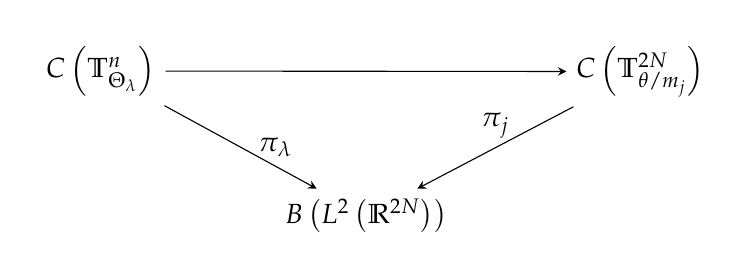
\begin{tikzpicture}
	\matrix (m) [matrix of math nodes,row sep=3em,column sep=4em,minimum width=2em]
	{
		C\left(\mathbb{T}^n_{\Theta_\la}\right) 	&   & C\left(\T^{2N}_{\th/m_{j}}\right) \\
		& B\left(L^2\left(\R^{2N}\right)\right) &  \\};
	\path[-stealth]
	(m-1-1) edge node [left] {} (m-1-3)
	(m-1-1) edge node [right] {$~\pi_\la$} (m-2-2)
	(m-1-3) edge node [above] {$\pi_{j}$}  (m-2-2);
	\end{tikzpicture}
	\newline
	yields a faithful representation $\widehat{\pi}:\widehat{C\left(\mathbb{T}^{n}_{\Th}\right) } \to  B\left(L^2\left(\R^{2N}\right)\right)$. There is the action of $\Z^{2N} \times \R^{2N} \to \R^{2N}$ given by
	$$
	\left(k, x \right) \mapsto k + x.
	$$
	The action naturally induces the action of $\Z^{2N}$ on both $L^2\left(\R^{2N}\right)$ and $B\left(L^2\left(\R^{2N}\right)\right)$. Otherwise the action of $\Z^{2N}$ on  $B\left(L^2\left(\R^{2N}\right)\right)$ induces the action  of $\Z^{2N}$ on $\widehat{C\left(\mathbb{T}^{2N}_{\th}\right) }$. There is the following commutative diagram
	\newline
	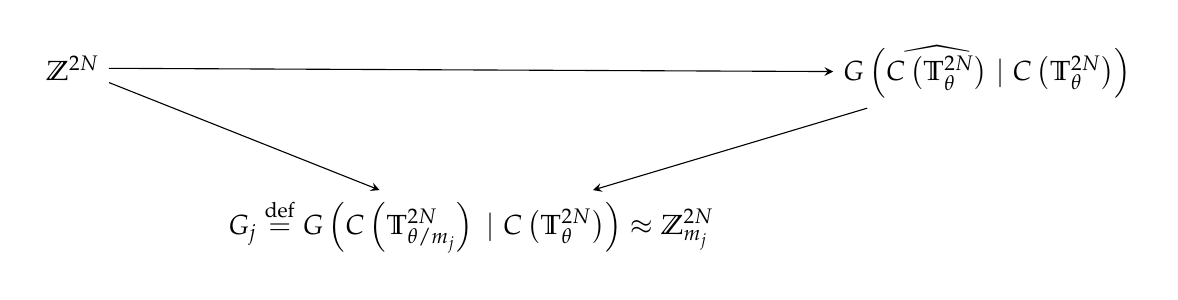
\begin{tikzpicture}
	\matrix (m) [matrix of math nodes,row sep=3em,column sep=4em,minimum width=2em]
	{
		\Z^{2N}	&   & G\left(\widehat{C\left(\T^{2N}_\th\right)}~|~ C\left(\mathbb{T}^{2N}_{\th}\right)\right) \\
		& G_j \bydef G\left(C\left(\T^{2N}_{\th/m_{j}}\right)~|~ C\left(\mathbb{T}^{2N}_{\th}\right)\right) \approx \Z^{2N}_{m_j}  &  \\};
	%\draw[dashed,->] (m-1-1) -- (m-1-3);
	\path[-stealth]
	(m-1-1) edge node [left] {} (m-1-3)
	(m-1-1) edge node [right] {} (m-2-2)
	(m-1-3) edge node [above] {}  (m-2-2);
	
	\end{tikzpicture}
	\newline
	Taking into account the  Definition \ref{compliant_covering_defn} and the Lemma \ref{nt_compliant_covering_lem} one has the following diagram
	\newline
	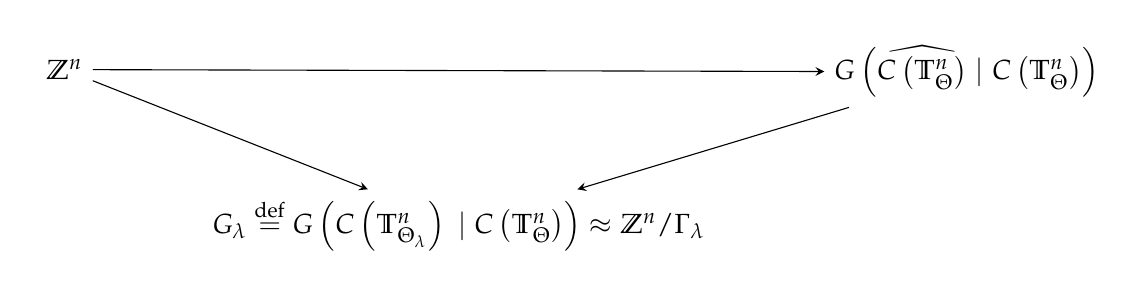
\begin{tikzpicture}
	\matrix (m) [matrix of math nodes,row sep=3em,column sep=4em,minimum width=2em]
	{
		\Z^{n}	&   & G\left(\widehat{C\left(\T^{n}_\Th\right)}~|~ C\left(\mathbb{T}^{n}_{\Th}\right)\right) \\
		&G_\la\bydef G\left(C\left(\T^{n}_{\Th_\la}\right)~|~  C\left(\mathbb{T}^{n}_{\Th}\right)\right) \approx \Z^{n}/\Ga_\la  &  \\};
	%\draw[dashed,->] (m-1-1) -- (m-1-3);
	\path[-stealth]
	(m-1-1) edge node [left] {} (m-1-3)
	(m-1-1) edge node [right] {} (m-2-2)
	(m-1-3) edge node [above] {}  (m-2-2);
	
	\end{tikzpicture}
	\newline	 
	%where $\phi_j$, $\varphi_j$ a group epimorphisms and the dashed arrow means the arrow to the inverse limit.
	If $\widehat G \bydef \varprojlim_{\la \in \La} G_\la$ then from the above diagram it follows that there is the natural homomorphism $\Z^{2N} \hookto \widehat{G}$, and 
	$\Z^{2N}$ is a normal subgroup.   Let  $J \subset \widehat{G}$  be a set of representatives of $\widehat{G}/\Z^{2N}$, and suppose that $0_{\widehat{G}} \in J$. 
	Any $g \in \widehat{G}$ can be uniquely represented as $g = g_J + g_\Z$ where  $g \in J$, $g_\Z \in \Z^{2N}$.  For any $g_1, g_2 \in \widehat{G}$ denote by $\Phi_J\left(g_1, g_2 \right) \in J$, $\Phi_\Z\left(g_1, g_2 \right) \in \Z^{2N}$, such that
	$$
	g_1 + g_2 = \Phi_J\left(g_1, g_2 \right) + \Phi_\Z\left(g_1, g_2 \right).
	$$
	Let us define an action of $\widehat{G}$ on  $\bigoplus_{g \in J}L^2\left(\R^{2N}\right)$ given by
	\be\label{nt_h_act_eqn}
	g_1  \left(0,..., \underbrace{ \xi}_{g_2^{\text{th}}-\text{place}},...,0,... \right) = \left(0,..., \underbrace{\Phi_\Z\left(g_1, g_2 \right)  \xi}_{\Phi_J\left(g_1 + g_2 \right) ^{\text{th}}-\text{place}},..., 0, ... \right).
	\ee
	Let $X \subset \bigoplus_{g \in J}L^2\left(\R^{2N}\right)$ be given by
	$$
	X = \left\{ \eta  \in \bigoplus_{g \in J}L^2\left(\R^{2N}\right)~|~   \eta=\left(0,..., \underbrace{ \xi}_{0_{\widehat{G}}^{\text{th}}-\text{place}},...,0,... \right) \right\}.
	$$
	Taking into account that $X \approx L^2\left(\R^{2N}\right)$, we will write $L^2\left(\R^{2N}\right) \subset \bigoplus_{g \in J}L^2\left(\R^{2N}\right)$ instead of $X \subset\bigoplus_{g \in J}L^2\left(\R^{2N}\right)$.
	This inclusion and the action of $\widehat{G}$ on $\bigoplus_{g \in J}L^2\left(\R^{2N}\right)$ enable us write $\bigoplus_{g \in J}gL^2\left(\R^{2N}\right)$ instead of $\bigoplus_{g \in J}L^2\left(\R^{2N}\right)$. If $\widehat{\pi}^\oplus: \widehat{C\left(\mathbb{T}^{2N}_{\th}\right) } \to B\left( \bigoplus_{g \in J}gL^2\left(\R^{2N}\right)\right)   $ is given by
	\be\label{nt_equiv_eqn}
	\widehat{\pi}^\oplus\left( a\right)\left(g\xi \right) =  g\left( \widehat{\pi}\left(g^{-1}a \right) \xi\right); ~ \forall a \in  \widehat{C\left(\mathbb{T}^{2N}_{\th}\right) }, ~ \forall g \in J,~ \forall \xi \in L^2\left(\R^{2N} \right). 
	\ee
\end{empt}
\subsection{Inverse noncommutative limit}\label{nt_inv_lim_sec}
\paragraph{}
Below we use the '$\times$' symbol for the Moyal plane product using  the described in \ref{mp_scaling_empt} scaling construction.
\begin{lem}\label{mp_ab_delta_lem}
	Let $a, b \in \SS\left(\R^{2N} \right)$. For any $\Delta \in \R^{2N}$ let $a_\Delta \in  \SS\left(\R^{2N} \right) $ be such that 
	\be\label{nt_a_delta_eqn}	
	a_\Delta\left(x \right)\stackrel{\mathrm{def}}{=} a\left(x + \Delta  \right).
	\ee For any $m, n \in \N$ there is a constant $A^{a,b}_{m, n}$ such that
	\be\label{mp_ab_delta_eqn}
	\begin{split}
		\left|  a_\Delta \diamond b \left( x\right) \right|< \frac{A^{a,b}_{m,n}}{\left( 1+\left\|\Delta \right\|\right)^m \left( 1+\left\|x \right\|\right)^n } \quad \forall x \in \R^{2N}\\
	\end{split}
	\ee
	where $\diamond$ means the given by \eqref{nt_diamond_eqn} twisted convolution.
\end{lem}
\begin{proof}
	
	From the definition of Schwartz functions it follows that for any $f \in \sS\left( \mathbb{R}^{2N} \right)$ and any $l\in \mathbb{N}$ there is $C^f_l>0$ such that
	\begin{equation}\label{nt_c_f_m_eqn}
	\left|f \left(u\right)\right|<\frac{C^f_l}{\left( 1 + \left\|u\right\|\right)^l }.
	\end{equation}
	Denote by $\Psi\left(x\right)\stackrel{\mathrm{def}}{=}\left| \sF\left( a_\Delta \times b\right) \left( x\right) \right|$
	From \eqref{mp_fourier_eqn} it follows that
	\bean
	\Psi\left(x, \Delta\right)=	 a_\Delta \diamond b\left(x \right)  =    	\int_{\R^{2N}}a_\Delta\left(x-t \right) b\left(t\right)e^{  i x \cdot J t }~dt =\\= \int_{\R^{2N}}a\left(x+\Delta -t \right) b\left(t\right)e^{  i x \cdot J t }~dt.
	\eean
	Consider two special cases:
	\begin{enumerate}
		\item[(i)] $\left\| x\right\| \le  \frac{\left\| \Delta\right\| }{2}$,
		\item[(ii)]	$\left\| x\right\| >  \frac{\left\| \Delta\right\| }{2}$.	
	\end{enumerate}	
	(i)		From \eqref{nt_c_f_m_eqn} it turns out
	\begin{equation}\label{mp_xi_1_eqn}
	\begin{split}
	\left| \Psi\left(x, \Delta \right)\right|  \le ~ \int \left|a\left(x+\Delta -t \right) b\left(t\right)e^{  i x \cdot J t } \right|dt \le\\
	\le
	\int_{\mathbb{R}^{2N}}\frac{C^{a}_{M}}{\left(1 + \left\|t - \Delta - x\right\|  \right)^{M}}~\frac{C^{b}_{2M}}{\left(1 + \left\|t\right\|  \right)^{2M}} dt =\\= \int_{\mathbb{R}^{2N}}\frac{C^{a}_{M}}{\left(1 + \left\|t - \Delta - x\right\|  \right)^{M}\left(1 + \left\|t\right\|  \right)^{M} }~\frac{C^{b}_{2M}}{\left(1 + \left\|t\right\|  \right)^{M}} dt  \le
	\\
	\le \sup_{x \in \mathbb{R}^{2N}, ~\left\| x\right\|\le \frac{\left\| \Delta\right\|}{2 },~s\in \mathbb{R}^{2N}}~ \frac{C^{a}_{M}C^{b}_{2M}}{\left(1 + \left\|s - \Delta - x\right\|  \right)^{M} \left(1 + \left\|s\right\|  \right)^{M}}
	\times \\ \times \int_{\mathbb{R}^{2N}}\frac{1}{\left(1 + \left\|t\right\|  \right)^{M}} dt.
	\end{split}
	\end{equation}
	If $x,y \in \mathbb{R}^{2N}$  then from the triangle inequality it follows that $\left\|x + y\right\|>  \left\|y\right\| - \left\|x\right\|$, hence 
	$$
	\left(1 + \left\|x\right\| \right)^M \left(1 + \left\|x+ y\right\| \right)^M \ge \left(1 + \left\|x\right\| \right)^M \left(1 +  \max\left(0, \left\|y\right\| - \left\|x\right\| \right)\right)^M.
	$$
	If $ \left\|x\right\| \le \frac{\left\|y\right\|}{2}$ then $\left\|y\right\| - \left\|x\right\| \ge \frac{\left\|y\right\|}{2}$ and 
	\begin{equation}\label{nt_triangle_eqn}
	\left(1 + \left\|x\right\| \right)^M \left(1 + \left\|x+ y\right\| \right)^M > \left( \frac{\left\|y\right\|}{2}\right)^M. 
	\end{equation}
	Clearly if $ \left\|x\right\| > \frac{\left\|y\right\|}{2}$ then condition \eqref{nt_triangle_eqn} also holds, hence\eqref{nt_triangle_eqn} is always true.
	It turns out from $\left\|-x-\Delta\right\|> \frac{\left\|\Delta\right\|}{2} $ and \eqref{nt_triangle_eqn} that
	$$
	\mathrm{inf}_{x \in \mathbb{R}^{2N}, ~\left\| x\right\|\le \frac{\left\| \Delta\right\|}{2 },~s\in \mathbb{R}^{2N}} \left(1 + \left\|s - \Delta - x\right\|  \right)^{M} \left(1 + \left\|s\right\|  \right)^{M} >\left\|\frac{\Delta}{4}\right\|^M,
	$$
	hence from \eqref{mp_xi_1_eqn} it turns out
	\be\nonumber
	\left| \Psi\left(x , \Delta\right)\right| \le \frac{4^MC^{a}_{M}C^{b}_{2M}}{\left\|\Delta\right\|^M} \times  \int_{\mathbb{R}^{2N}}\frac{1}{\left(1 + \left\|t\right\| \right)^{M}} dt = \frac{C'}{\left\|\Delta\right\|^M}
	\ee
	where
	\be\label{nt_c'_eqn}
	C' = 4^MC^{a}_{M}C^{b}_{2M}  \int_{\mathbb{R}^{2N}}\frac{1}{\left(1 + \left\|t\right\| \right)^{M}}.
	\ee
	Otherwise from
	$$
	\left(1 + \left\|s - \Delta - x\right\|  \right)^{M} \left(1 + \left\|s\right\|  \right)^{M} > 1
	$$
	it follows that $
	\Psi\left(x , \Delta\right) \le C'$ and taking into account \eqref{nt_c'_eqn} one has
	$$
	\left| 	\Psi\left(x , \Delta\right)\right| \le \frac{2C'}{\left( 1 + \left\|\Delta\right\|\right) ^M}
	$$
	If $M = 2M'$ then from $\left\| x\right\|  \le \frac{\Delta}{2}$ it follows that
	\be\label{nt_c''_eqn}
	\left| \Psi\left(x , \Delta\right)\right| \le \frac{2C'2^{M'}}{\left( 1 + \left\|\Delta\right\|\right) ^{M'} \left( 1 + \left\|x\right\|\right)^{M'} }.
	\ee
	If $M$ is such that $M > 2n$ and $M > 2m$ then from \eqref{nt_c''_eqn} it follows that 
	\be\label{nt_c'''_eqn}
	\Psi\left(x , \Delta\right)\le \frac{4C'2^{M'}}{\left( 1 + \left\|\Delta\right\|\right)^m  \left( 1 + \left\|x\right\|\right)^n }.
	\ee
	(ii)
	If $\left( \cdot, \cdot \right)_{L^2\left(\R^{2N} \right) }$ is the given by \eqref{fourier_scalar_product_eqn} scalar product then from \eqref{mp_inv_eqn} it turns out
	\begin{equation*}
	\begin{split}
	\left| \Psi\left(x , \Delta\right) \right|\le\left|\int a\left( t - \Delta - x \right)  b\left(t \right)e^{i x \cdot J t}  dt\right|=\\
	=\left|\left(    a\left( \bullet- \Delta-x\right) ,~ b\left(\bullet\right)e^{i x\cdot J\bullet}   \right)_{L^2\left(\R^{2N} \right) }  \right|=\\
	=\left|\left(  \mathcal{F}\left(  a\left( \bullet- \Delta-x\right)\right) ,~ \mathcal{F}\left( b\left(\bullet\right)e^{i x\cdot J\bullet} \right)  \right)_{L^2\left(\R^{2N} \right) }  \right|=\\=
	\left|\int_{\mathbb{R}^{2N}} 
	\mathcal{F}\left( a\right)\left( \bullet - \Delta -x\right)\left(u\right)\mathcal{F}\left(b\left(\bullet\right)e^{i x\cdot J\bullet} \right)\left(u\right)  du \right|\le\\
	\le \int_{\mathbb{R}^{2N}}\left| e^{-i\left(-\Delta - x\right) \cdot u}\mathcal{F}\left( a\right)\left( u\right) \mathcal{F}\left(b\right)\left(u+J x\right)\right| du \le \\
	\le \int_{\mathbb{R}^{2N}}\frac{C^{\mathcal{F}\left( a\right)}_{3M}}{\left(1 + \left\|u\right\|  \right)^{3M}}\frac{C^{\mathcal{F}\left(b\right)}_{2M}}{\left(1 + \left\|u-J x\right\|  \right)^{2M}} du \le \\
	\le \sup_{x \in \mathbb{R}^{2N}, ~\left\| x\right\|> \frac{\left\| \Delta\right\|}{2 },~ s \in \mathbb{R}^{2N}}~ \frac{C^{\mathcal{F}\left( a\right)}_{3M}}{\left(1 + \left\|s\right\|  \right)^{M}}
	\frac{C^{\mathcal{F}\left(b\right)}_{2M}}{\left(1 + \left\|s-J x\right\|  \right)^{M}} \times \\ \times    
	\frac{1}{\left(1 + \left\|u-J  x\right\|  \right)^{M}\left(1 + \left\|u\right\|  \right)^{M}}\int_{\mathbb{R}^{2N}}\frac{1}{\left(1 + \left\|u\right\|  \right)^{M}} du.
	\end{split}
	\end{equation*}
	From \eqref{nt_triangle_eqn} it follows that
	\begin{equation*}
	\begin{split}
	\left(1 + \left\|u\right\|  \right)^{M}\left(1 + \left\|u-J x\right\|  \right)^{M} > \left\|J x\right\|^M, 
	\\
	\inf_{x \in \mathbb{R}^{2N}, ~\left\| x\right\|> \frac{\left\| \Delta\right\|}{2 },~ s \in \mathbb{R}^{2N}}~ \left(1 + \left\|s\right\|  \right)^{M}\left(1 + \left\|s-J x\right\|  \right)^{M} > \left\|\frac{J\Delta}{4}\right\|^M,\\
	\end{split}
	\end{equation*}
	and taking into account 	$\left(1 + \left\|u\right\|  \right)^{M}\left(1 + \left\|u-J x\right\|  \right)^{M}  \ge 1$, $\left(1 + \left\|s\right\|  \right)^{M}\left(1 + \left\|s-J x\right\|  \right)^{M}  > 1$ one has
	\begin{equation*}
	\begin{split}
	\left| \Psi\left(x , \Delta\right)   \right|
	\le  \frac{C^{\mathcal{F}\left( a\right)}_{3M}C^{\mathcal{F}\left(b\right)}_{2M}}{\left\|\frac{\Delta}{4}\right\|^M \left\|J x\right\|^M} \int_{\R^{2N}}\frac{1}{\left(1+\left\|u\right\| \right)^M }du,\\
	\left| \Psi\left(x , \Delta\right)   \right|
	\le  C^{\mathcal{F}\left( a\right)}_{3M}C^{\mathcal{F}\left(b\right)}_{2M}\int_{\R^{2N}}\frac{1}{\left(1+\left\|u\right\| \right)^M }du
	\end{split}
	\end{equation*}
	If  $M > 2N + m$ then the integral $I=\int_{\R^{2N}}\frac{1}{\left(1+\left\|u\right\| \right)^M }du$ is convergent and from 
	\be\label{mp_psi_big_eqn}
	\begin{split}
		\left| \Psi\left(x , \Delta\right)   \right|
		\le  \frac{4C^{\mathcal{F}\left( a\right)}_{3M}C^{\mathcal{F}\left(b\right)}_{2M}I}{\left\|\left(1+ \frac{\Delta}{4}\right\|\right)^M \left( 1+\left\|J x\right\|\right)^M},\\
	\end{split}	
	\ee
	From \eqref{nt_simpectic_theta_eqn} and $\th = 2$ one has
	$
	\left\|J z\right\|= \left\|2 z\right\|; ~ \forall z \in \R^{2N}
	$  and taking into account \eqref{mp_psi_big_eqn} there is $C_1 > 0$ such that
	\be\label{mp_psi_two_eqn}
	\begin{split}
		\left| \Psi\left(x , \Delta\right)   \right|
		\le  \frac{C_1}{\left\|\left(1+ \Delta\right\|\right)^M \left( 1+\left\| x\right\|\right)^M},\\
	\end{split}	
	\ee
	If $M \ge m$ and $M \ge n$ then from \eqref{mp_psi_two_eqn} it turns out 
	\be\label{mp_psip_two_eqn}
	\begin{split}
		\left| \Psi\left(x , \Delta\right)   \right|
		\le  \frac{2C_1}{\left\|\left(1+ \Delta\right\|\right)^m \left( 1+\left\| x\right\|\right)^n},\\
	\end{split}	
	\ee
	If $A^{a,b}_{m,n} \in \R$ is such that $A^{a,b}_{m,n} \ge 4C'2^{M'}$ and $A^{a,b}_{m,n} \ge 2C_1$
	then from \eqref{nt_c'''_eqn} and \eqref{mp_psip_two_eqn} it follows that  $A^{a,b}_{m,n}$ satisfies to \eqref{mp_ab_delta_eqn}.
\end{proof}
\begin{corollary}\label{mp_ab_deltad_cor}
	Let $a, b \in \SS\left(\R^{2N} \right)$. For any $\Delta \in \R^{2N}$ let $a_\Delta \in  \SS\left(\R^{2N} \right) $ be such that $a_\Delta\left(x \right)\stackrel{\mathrm{def}}{=} a\left(x + \Delta  \right)$. For any $m, n \in \N$ there is a constant $C^{a,b}_{m, n}$ such that
	\be\label{mp_ab_deltad_eqn}
	\begin{split}
		\left|\left(  a_\Delta \diamond b\right)  \left( x\right) \right|< \frac{C^{a,b}_{m,n}}{\left( 1+\left\|\Delta \right\|\right)^m \left( 1+\left\|x \right\|\right)^n },\\
		\left|\left(  b\diamond a_\Delta \right)  \left( x\right) \right|< \frac{C^{a,b}_{m,n}}{\left( 1+\left\|\Delta \right\|\right)^m \left( 1+\left\|x \right\|\right)^n },\\
		\left|\left(  a_\Delta \times b\right)  \left( x\right) \right|< \frac{C^{a,b}_{m,n}}{\left( 1+\left\|\Delta \right\|\right)^m \left( 1+\left\|x \right\|\right)^n },\\
		\left|\left(  b\times a_\Delta \right)  \left( x\right) \right|< \frac{C^{a,b}_{m,n}}{\left( 1+\left\|\Delta \right\|\right)^m \left( 1+\left\|x \right\|\right)^n },\\	
		\left|\mathcal F \left(  a_\Delta \diamond b\right)  \left( x\right) \right|< \frac{C^{a,b}_{m,n}}{\left( 1+\left\|\Delta \right\|\right)^m \left( 1+\left\|x \right\|\right)^n },\\
		\left|\mathcal F\left(  b\diamond a_\Delta \right)  \left( x\right) \right|< \frac{C^{a,b}_{m,n}}{\left( 1+\left\|\Delta \right\|\right)^m \left( 1+\left\|x \right\|\right)^n },\\
		\left|\mathcal F\left(  a_\Delta \times b\right)  \left( x\right) \right|< \frac{C^{a,b}_{m,n}}{\left( 1+\left\|\Delta \right\|\right)^m \left( 1+\left\|x \right\|\right)^n },\\
		\left|\mathcal F\left(  b\times a_\Delta \right)  \left( x\right) \right|< \frac{C^{a,b}_{m,n}}{\left( 1+\left\|\Delta \right\|\right)^m \left( 1+\left\|x \right\|\right)^n }.\\
	\end{split}
	\ee
	where $\sF$ means the Fourier transformation.
\end{corollary}
\begin{proof}
	From the Lemma \ref{mp_ab_deltad_eqn} it follows that is a constant $A^{a,b}_{m, n}$ such that
	$$
	\left|\left(  a_\Delta \diamond b\right)  \left( x\right) \right|< \frac{A^{a,b}_{m,n}}{\left( 1+\left\|\Delta \right\|\right)^m \left( 1+\left\|x \right\|\right)^n }.
	$$
	
	Clearly  $\left| b \diamond a_\Delta   \left( x\right) \right|=\left|\left( b \diamond a_\Delta \right)^*  \left( x\right) \right|= $ and taking into account  \eqref{nt_prod_*_eqn} one has
	\be\label{mp_*_eqn}
	\left| b \diamond a_\Delta   \left( x\right) \right|= \left|\left( b \diamond a_\Delta \right)^*  \left( x\right) \right|= \left|\left(  a^*_\Delta \diamond b^*\right)  \left( x\right) \right|< \frac{A^{b^*,a^*}_{m,n}}{\left( 1+\left\|\Delta \right\|\right)^m \left( 1+\left\|x \right\|\right)^n }
	\ee
	From \eqref{nt_prodf_duality} it follows that
	$$
	a_\Delta \times b = a_\Delta \diamond \widetilde F b,
	$$
	hence from the Lemma \ref{mp_ab_deltad_eqn} it follows that
	$$
	\left|  a_\Delta \times b  \left( x\right) \right| < \frac{A^{a,\widetilde F b}_{m,n}}{\left( 1+\left\|\Delta \right\|\right)^m \left( 1+\left\|x \right\|\right)^n }
	$$
	Similarly to \eqref{mp_*_eqn} one has
	$$
	\left| b \times a_\Delta   \left( x\right) \right| < \frac{A^{\left( \widetilde F b\right)^*, a^* }_{m,n}}{\left( 1+\left\|\Delta \right\|\right)^m \left( 1+\left\|x \right\|\right)^n }
	$$
	Applying \eqref{nt_prod_duality_eqn} one has
	\bean
	\left|\mathcal F \left(  a_\Delta \diamond b\right)  \left( x\right) \right|< \frac{A^{\mathcal F a, ~\mathcal F\widetilde F b}_{m,n}}{\left( 1+\left\|\Delta \right\|\right)^m \left( 1+\left\|x \right\|\right)^n },\\
	\left|\mathcal F\left(  b\diamond a_\Delta \right)  \left( x\right) \right|< \frac{A^{\sF\left( \widetilde F b\right)^*, \sF a^*}_{m,n}}{\left( 1+\left\|\Delta \right\|\right)^m \left( 1+\left\|x \right\|\right)^n },\\
	\left|\mathcal F\left(  a_\Delta \times b\right)  \left( x\right) \right|< \frac{A^{\mathcal F a,\mathcal F b}_{m,n}}{\left( 1+\left\|\Delta \right\|\right)^m \left( 1+\left\|x \right\|\right)^n },\\
	\left|\mathcal F\left(  b\times a_\Delta \right)  \left( x\right) \right|< .
	\eean
	If $C^{a, b}_{m,n} \in \R$ is such that
	\bean
	C^{a, b}_{m,n} > A^{a,~ b}_{m,n}, \quad C^{a, b}_{m,n} > A^{b^*, ~a^*}_{m,n}, \quad C^{a, b}_{m,n} > A^{a, ~\widetilde F b}_{m,n}, \quad C^{a, b}_{m,n} > A^{\left( \widetilde F b\right)^*, ~a^* }_{m,n},\\
	C^{a, b}_{m,n} > A^{\sF a,~ \sF  b}_{m,n}, \quad C^{a, b}_{m,n} > A^{\sF b^*, ~\sF a^*}_{m,n}, \quad C^{a, b}_{m,n} > A^{\sF a, ~\sF \widetilde F b}_{m,n}, \quad C^{a, b}_{m,n} > A^{\left( \sF \widetilde F b\right)^*, ~\sF a^* }_{m,n}
	\eean
	then from the above construction it follows that $C^{a, b}_{m,n}$ satisfies to the equations \eqref{mp_ab_deltad_eqn}.
\end{proof}

\begin{corollary}\label{mp_ab_delta_cor}
	Let $a, b \in \SS\left(\R^{2N} \right)$. For any $\Delta \in \R^{2N}$ let $a_\Delta \in  \SS\left(\R^{2N} \right) $ be such that $a_\Delta\left(x \right)= a\left(x + \Delta  \right)$. For any $m \in \N$ there is a constant $C^{a,b}_m$ such that for any $x, \Delta \in \R^{2N}$ following conditions hold
	\be\label{mp_ab_delta_cor_eqn}
	\left\| a_\Delta \times b\right\|_2 < \frac{C^{a,b}_m}{\left( 1+\left\|\Delta \right\|\right)^m  }
	\ee
	where $\left\| \cdot\right\|_2$ is given by \eqref{nt_l2_norm_eqn}.
\end{corollary}
\begin{proof}
	Follows from the equation \ref{mp_ab_deltad_eqn}.
\end{proof}

\begin{lemma}\label{nt_w*_top_lem}
	If $\overline a \in S\left(\R^{2N}\right)$ then for all $j\in \N$ the following conditions hold:
	\begin{enumerate}
		\item [(i)] The series 	
	\be\label{nt_w*_top_eqn}
		\sum_{g \in \ker\left( \Z^{2N} \to \Z^{2N}_{m_j}\right) }  g \overline a = a_j
	\ee
		is convergent with respect to the weak*-topology (cf. Definition \ref{w*_topology_defn}) of the dual space $S'\left(\R^{2N}\right)$ of $ S\left(\R^{2N}\right)$. Moreover $a_j$ is represented by infinitely differentiable map $\R^{2N}\to \C$, i.e. $a_j\in \Coo\left(\R^{2N} \right)$.
		\item[(ii)] One has 
		\be\label{mp_fourier_torusa_eqn}
	a_j = \sum_{k \in Z^{2N}} c_k \exp\left(2\pi i \frac{k}{m_j} ~\cdot \right)
		\ee
		where $\left\{c_k \in \C\right\}_{k \in \Z^{2N}}$ are rapidly decreasing coefficients given by
		\begin{equation}\label{mp_fourier_torus_eqn}
		c_k = \frac{1}{m_j^{2N} } \int_{\R^{2N}} \overline{a}\left(x \right)  \exp\left(2\pi i \frac{k}{m_j}\cdot x\right) dx = \frac{1}{m_j^{2N} } \mathcal{F}\overline{a}\left( \frac{k}{m_j}\right)   .
		\end{equation}
	\end{enumerate}
\end{lemma}
\begin{proof}
Let $I \bydef \left[0, m_j \right]^{2N}\subset \R^{2N}$ be a cube.
If $R \bydef \sqrt{2N} m_j$  then $\left\|x \right\| < R$  for all $x\in I$, hence from \eqref{nt_ineqr_eqn} it follows that
$$
\left| \left( g \overline a\right) \left( x\right) \right|= \left|  \overline a\left( x+ g\right) \right|< \frac{C^{m,R}_f}{\left(1 + \left\|g \right\|^{m}\right) }\quad\forall x\in I.
$$
For all $m > 2N$ the series $\sum_{g \in \ker\left( \Z^{2N} \to \Z^{2N}_{m_j}\right) }\frac{C^{m,R}_f}{\left(1 + \left\|g \right\|^{m}\right) }$ is convergent. If 
$$C \bydef \sum_{g \in \ker\left( \Z^{2N} \to \Z^{2N}_{m_j}\right) }\frac{C^{m,R}_f}{\left(1 + \left\|g \right\|^{m}\right) }$$ then for any subset $G\subset \ker\left( \Z^{2N} \to \Z^{2N}_{m_j}\right)$ and $x \in I$ one has 
\be
\left| \sum_{g \in G } \left( g \overline a\right) \left( x\right)\right| < C.
\ee
Moreover the series 
$$
\sum_{g \in \ker\left( \Z^{2N} \to \Z^{2N}_{m_j}\right) }\left. \left( g \overline a\right)\right|_{I}
$$
is uniformly convergent, so the sum of the above series is continuous. If $D^{\beta} = \frac{\partial}{\partial x_1^{\bt_1}}~...~\frac{\partial}{\partial x_n^{\bt_n}}$ then from the equation \eqref{mp_sr_eqn} it turns out that $D^{\beta}\overline a \in \SS\left(\R^{2N}\right)$, so the sum of the series
$$
\sum_{g \in \ker\left( \Z^{2N} \to \Z^{2N}_{m_j}\right) }\left. \left( g  D^\bt\overline a\right)\right|_{I}
$$
is also continuous. If $\eps > 0$ and $a \in \SS\left(\R^{2N}\right)$ then there is a compact set $\sV \subset \R^{2N}$ such that $\left|a\left( x\right)  \right|< \frac{\eps}{2C}$ for all $\R^{2N}\setminus\sV$. There is a finite subset $G_0 \subset\ker\left( \Z^{2N} \to \Z^{2N}_{m_j}\right)$ such that $\sV\subset \bigcup_{g\in G_0}gI$. Denote by $C_a\bydef \sup_{x \in \R^{2N}}\left|a \left( x\right)\right|$. Otherwise there is a finite set $G_I\subset\ker\left( \Z^{2N} \to \Z^{2N}_{m_j}\right)$ such that
$$
G_I\subset G \subset \ker\left( \Z^{2N} \to \Z^{2N}_{m_j}\right)\quad \Rightarrow\quad \left\| \sum_{g \in \ker\left( \Z^{2N} \to \Z^{2N}_{m_j}\right) }\left. \left( g \overline a\right)\right|_{I}- \sum_{g \in G }\left. \left( g \overline a\right)\right|_{I} \right\|< \frac{\eps}{2C_a} 
$$
For any $g' \in G_0$ one has
\bean
gG_I\subset G \subset \ker\left( \Z^{2N} \to \Z^{2N}_{m_j}\right)\quad \Rightarrow\\
\Rightarrow\quad\left\| \sum_{g \in \ker\left( \Z^{2N} \to \Z^{2N}_{m_j}\right) }\left. \left( g \overline a\right)\right|_{g'I}- \sum_{g \in g'G_I }\left. \left( g \overline a\right)\right|_{g'I} \right\|< \frac{\eps}{2C_a} 
\eean
If $\overline G \bydef \bigcup_{g'\in G_0} g'G_I$ then from above construction it follows that
$$
\overline G \subset G \subset \ker\left( \Z^{2N} \to \Z^{2N}_{m_j}\right)\quad \Rightarrow\quad \left| \left\langle \sum_{g \in \ker\left( \Z^{2N} \to \Z^{2N}_{m_j}\right) } g \overline a, a\right\rangle- \left\langle \sum_{g \in \overline G} g \overline a, a\right\rangle \right|< \eps, 
$$ 
i.e. the series \ref{nt_w*_top_eqn} is convergent with respect to the weak*-topology. The sum of series is periodic and since the sums $\sum_{g \in \ker\left( \Z^{2N} \to \Z^{2N}_{m_j}\right) }\left.  g \overline a\right|_{I}$ and $\sum_{g \in \ker\left( \Z^{2N} \to \Z^{2N}_{m_j}\right) }\left. \left( g \overline D^\bt a\right)\right|_{I}$ are continuous $a_j$ is represented by infinitely differentiable map $\R^{2N}\to \C$.\\
(ii) Follows from
\bean 
c_k = \frac{1}{m_j^{2N} }\int_I \exp\left(2\pi i \frac{k}{m_j} ~x \right)\sum_{g \in\ker\left( \Z^{2N} \to \Z^{2N}_{m_j}\right)}\left( g \overline a\right)\left( x\right) dx  =\\
= \frac{1}{m_j^{2N} }\sum_{g \in\ker\left( \Z^{2N} \to \Z^{2N}_{m_j}\right)}\int_{gI}\exp\left(2\pi i \frac{k}{m_j} ~x \right) \overline a\left(x\right)dx=\\= \frac{1}{m_j^{2N} }\int_{\R^{2N}}\exp\left(2\pi i \frac{k}{m_j} ~x \right)\overline a\left(x\right)dx= \frac{1}{m_j^{2N} } \mathcal{F}\overline{a}\left( \frac{k}{m_j}\right).
\eean
\end{proof}




\begin{lemma}\label{nt_w*_lem}
If $\overline a \in S\left(\R^{2N} _\th\right)$ is an element which correspond to positive element of $C_b\left( \R^{2N}_\th\right)\subset B\left( L^2\left(\R^{2N}_\th \right) \right)$ (cf. Definition \ref{nt_r_2_N_repr_defn}) then for all $j\in \N$ there is $a_j\in\Coo\left(\T^{2N}_{\th/2m_j}\right)$ such that the series
$$
\sum_{g \in \ker\left( \Z^{2N} \to \Z^{2N}_{m_j}\right) }  g \overline a = a_j
$$
is strongly convergent in $B\left( L^2\left(\R^{2N}_\th \right)\right)$. Moreover the sum of the above series in sense of the strong topology coincides with the sum with respect to the weak*-topology of the dual space $\sS'\left(\R^{2N}\right)$ (cf. Definition \ref{w*_topology_defn}).
\end{lemma}
\begin{proof}
	From the Lemma \ref{nt_w*_top_lem} it follows that there the series
\be\label{nt_sp_eqn}
\sum_{g \in \ker\left( \Z^{2N} \to \Z^{2N}_{m_j}\right) }  g \overline a = a_j\in S'\left(\R^{2N}\right)
\ee
is convergent with respect to the weak*-topology (cf. Definition \ref{w*_topology_defn}). Since $a_j$ is a smooth $m_j$ - periodic function it can be regarded as the element of $\Coo\left(\T^{2N}_{\th/2m_j}\right)$.	
 On the other hand from \ref{mp_nt_op_empt} it follows that $a_j \in C_b\left( \R^{2N}_\th\right)\subset  B\left( L^2\left(\R^{2N}_\th \right) \right)$. 
From \eqref{mp_star_ext_eqn} for any $x \in \SS\left(\R^{2N}_\th\right)$ and $g \in \ker\left( \Z^{2N} \to \Z^{2N}_{m_j}\right)$ one has
 \bean
 \left(x, \left( g \overline a\right)  x\right)_{L^2\left(\R^{2N}_\th \right) }= \left(\left( g \overline a\right)  x,  x\right)_{L^2\left(\R^{2N}_\th \right) }= \left(\left( g \overline a\right)\star_\th  x,  x\right)_{L^2\left(\R^{2N}_\th \right) }=\\
= \left\langle \left( \left( g \overline a\right)\star_\th  x\right)^* ,x \right\rangle= \left\langle x^*\star_{\th} \left( g \overline a\right) ,x \right\rangle=
  \left\langle g \overline a,x\star_{\th} x^* \right\rangle
 \eean
 where $\left(\cdot , \cdot \right)_{L^2\left(\R^{2N}_\th \right) }$ is the  scalar product of the Hilbert space and $\left\langle\cdot ,\cdot \right\rangle$ means the natural pairing  $\SS'\left(\R^{2N}_\th\right)\times \SS\left(\R^{2N}_\th\right)\to \C$. Since $g \overline a$ is a positive operator of $B\left( L^2\left(\R^{2N}_\th \right) \right)$ all summands of the series
 $$
 \sum_{g \in \ker\left( \Z^{2N} \to \Z^{2N}_{m_j}\right) } \left(x, g \overline a x\right)_{L^2\left(\R^{2N}_\th \right) }= \sum_{g \in \ker\left( \Z^{2N} \to \Z^{2N}_{m_j}\right) }\left\langle g \overline a,x\star_{\th} x^* \right\rangle
 $$ 
are positive. Otherwise  the series \eqref{nt_sp_eqn} is convergent with respect to the weak*-topology, so one has
\be\label{ctr_axx_eqn}
\sum_{g \in \ker\left( \Z^{2N} \to \Z^{2N}_{m_j}\right) }\left\langle g \overline a,x\star_{\th} x^* \right\rangle=\left\langle a_j,x\star_{\th} x^* \right\rangle
\ee
From the positivity of summands it follows that
$$
\sum_{g \in G } \left(x, g \overline a x\right)_{L^2\left(\R^{2N}_\th \right) }\le \left(x, a_j x\right)_{L^2\left(\R^{2N}_\th \right)}
$$
for any finite $G \subset  \ker\left( \Z^{2N} \to \Z^{2N}_{m_j}\right)$. Otherwise $\SS\left(\R^{2N}_\th\right)$ is dense subset of $L^2\left(\R^{2N}_\th\right)$ with respect to the Hilbert norm of $L^2\left(\R^{2N}_\th\right)$, so one has
$$
\sum_{g \in G' } \left(\xi, g \overline a \xi\right)_{L^2\left(\R^{2N}_\th \right) }\le \left(\xi, a_j \xi\right)_{L^2\left(\R^{2N}_\th \right)}
$$
for all $\xi\in L^2\left(\R^{2N}_\th \right)$, hence
$$
\sum_{g \in G' }  g \overline a \le a_j.
$$
So from the Lemma \ref{increasing_convergent_w_lem} it follows that the series $\sum_{g \in \ker\left( \Z^{2N} \to \Z^{2N}_{m_j}\right) } g \overline a$ is strongly convergent in $B\left( L^2\left(\R^{2N}_\th \right)\right)$. Moreover since $\sS\left( \R^{2N}\right)$ is dense in  $L^2\left( \R^{2N}\right)$ and taking into account the Equation \eqref{ctr_axx_eqn} one has
$$
\forall\xi \in L^2\left( \R^{2N}\right)\quad \sum_{g \in \ker\left( \Z^{2N} \to \Z^{2N}_{m_j}\right) } \left(\xi, g \overline a \xi\right)_{L^2\left(\R^{2N}_\th \right) }= \left(\xi, a_j \xi\right)_{L^2\left(\R^{2N}_\th \right)},
	$$
it turns out that
$$
\sum_{g \in \ker\left( \Z^{2N} \to \Z^{2N}_{m_j}\right) }  g \overline a = a_j
$$
where the sum of the series means the strong convergence in $B\left( L^2\left(\R^{2N}_\th \right)\right)$. 
\end{proof}

\begin{lemma}\label{nt_cmn_lem}
	If $m > n$ then there is $C^{m,n} > 0$ such that for any $k \in \N$ one has
	\be\label{nt_int_sum}
	s_k = \frac{1}{k^n}	\sum_{x \in \Z^n} \frac{1}{\left(1 + \left\|\frac{x}{k} \right\|  \right)^m} < C^{m,n}
	\ee
\end{lemma}
\begin{proof}
	If $f: \R^n \to \R$ and $\phi_k :\R^n \to \Z^n$ are given by
	\bean
	f\left( x\right) = \frac{1}{\left(1 + \left\|x\right\|  \right)^m},\\
	\phi_k\left(x_1, ..., x_n \right) = \left(y_1, ..., y_n \right)\in \Z^n,\quad 
	y_j \le kx_j < y_{j}+1 \quad j =1,..., n
	\eean
	then one has
	$$
	s_k = \int_{\R^n} f\left(\phi_k\left(\frac{x}{k} \right)  \right) dx.
	$$
	Otherwise from
	$$
	f\left(\phi_k\left(\frac{x}{k} \right) \right) \le 2^m f\left(x \right) \quad \forall x \in \R^n 
	$$
	it follows that
	$$
	s_k <   \int_{\R^n}\frac{2^m}{\left(1 + \left\|x\right\|  \right)^m}dx.
	$$
	From $m > n$ it follows that the integral $\int_{\R^n}\frac{1}{\left(1 + \left\|x\right\|  \right)^m}dx$ is convergent so one can assume
	$$
	C^{m,n} = \int_{\R^n}\frac{2^m}{\left(1 + \left\|x\right\|  \right)^m}dx
	$$
\end{proof}
\begin{corollary}\label{nt_cmn_cor}
	Let  $m > 2N$ and  $\widetilde{a} \in \SS\left( \R^{2N}_\th\right)$ is such that $$\left\| \sF \widetilde{a}\left(x \right)  \right\| < \frac{1}{\left(1 + \left\|x\right\|  \right)^m}
	$$
	For any $j \in \N$ following condition holds
	$$
	a_j = \sum_{g \in \ker\left( \Z^{2N} \to \Z^{2N}_{m_j}\right) } \widetilde{a} \quad \Rightarrow \left\| a_j \right\| < C^{m,n}
	$$
	where $C^{m,n}$ is given by the Lemma \ref{nt_cmn_lem}.
\end{corollary}
\begin{proof}
	From  \eqref{mp_fourier_torusa_eqn} and \eqref{mp_fourier_torus_eqn} it follows that
	$$
	\left\| a_j \right\| <  \frac{1}{m_j^{2N} } \sum_{k \in \Z^{2N}}\left\|\mathcal{F}\widetilde{a}\left( \frac{k}{m_j}\right) \right\| 
	$$
	and taking into account the Lemma  \ref{nt_cmn_lem} one has
	$$
	\left\| a_j \right\| < C^{m,n}
	$$
\end{proof}
\begin{corollary}
	If $m > n$ then 
	\be\label{nt_int_cor_sum}
	s = 	\sum_{x \in \Z^n \setminus 0} \frac{1}{\left\|x\right\|^m} < \infty
	\ee
\end{corollary}
\begin{proof}
	Follows from the Lemma \ref{nt_cmn_lem} and the implication 
	$$
	\left\|x\right\| > 1 \Rightarrow	\frac{1}{\left\|x\right\|^m} < \frac{2^m}{\left(1 + \left\|x\right\|  \right)^m}
	$$
\end{proof}





Denote by $\H^\oplus\bydef\bigoplus_{g \in J}gL^2\left(\R^{2N}\right)$ and let $\widehat{\pi}^\oplus: \widehat{C\left(\mathbb{T}^{2N}_{\th}\right) }  \hookto B\left( \H^\oplus\right)$ be given by \eqref{nt_equiv_eqn} representation.
If $\widetilde{a} \in \SS\left( \R^{2N}_\th\right)$ then from the Lemma \ref{spec_strong_lim_lem} it turns out
$\widetilde a \in \pi^\oplus\left( \widehat{C\left( \T^{2N}_\th\right) }\right) ''$. Since $\widehat{\pi}^\oplus$ is a faithful representation of $\widehat{C\left( \T^{2N}_\th\right) }$, one has  an injective homomorphism  $\SS\left( \R^{2N}_\th\right) \hookto \widehat{\pi}^\oplus\left( \widehat{C\left( \T^{2N}_\th\right) }\right) ''$ of involutive algebras. 
For any $\widetilde{a} \in \SS\left( \R^{2N}_\th\right)$ following condition holds
$$
\sum_{g \in \ker\left(\widehat{G} \to G_j\right)}g\widehat{\pi}^\oplus\left(\widetilde{a} \right) = \sum_{g' \in J}g'\left( \sum_{ g''\in \ker\left(\Z^{2N} \to G_j\right)}  g''\widehat{\pi}^\oplus\left(\widetilde{a} \right)\right)= \sum_{g \in J}gP. 
$$
where 
$$
P = \sum_{ g\in \ker\left(\Z^{2N} \to G_j\right)}  g\widehat{\pi}\left(\widetilde{a} \right).
$$


If $J \subset \widehat{G}$ is a set of  representatives of $\widehat{G}/\Z^{2N}$ and $g',g'' \in J$ are such that $g' \neq g''$ then operators $g'P$, $g''P$ act on mutually orthogonal Hilbert subspaces $g'L^2\left( 
R^{2N}\right)$, $g''L^2\left( 
R^{2N}\right)$ of the direct sum $\bigoplus_{g \in J} gL^2\left( 
R^{2N}\right)$, and 
taking into account $\left\|P\right\|=\left\|gP\right\|$  one has
\begin{equation}\label{nt_norm_equ_eqn}
\left\|\sum_{g \in \ker\left(\widehat{G} \to G_j\right)}\widehat{\pi}^\oplus\left( \widetilde{a} \right)\right\|= \left\|\sum_{g \in J}gP\right\|=\left\|P\right\|=\left\|\sum_{g \in \ker\left(\Z^{2N} \to G_j\right)}\widehat{\pi}\left( \widetilde{a} \right)\right\|.
\end{equation}


\begin{lem}\label{nt_w_spec_p_lem} 
	If $\overline{a}$ in $ \sS\left(\mathbb{R}^{2N}_\th \right) $ is positive then following conditions hold:
	\begin{enumerate}	
		\item[(i)]
		For any $j \in \mathbb{N}^0$ the following  series 
		\begin{equation*}
		\begin{split}
		a_j = \sum_{g \in \ker\left( \widehat{G} \to  G_j\right) )} g \overline{a},\\
		b_j = \sum_{g \in \ker\left( \widehat{G} \to  G_j\right) } g  \overline{a}^2
		\end{split}
		\end{equation*}
		are strongly convergent and the sums lie in   $\Coo\left( \T^{2N}_{\th/m_j^2}\right) $, i.e. $a_j, b_j \in \Coo\left( \T^{2N}_{\th/m_j^2}\right) $; 
		\item[(ii)] For any $\eps > 0$ there is $N \in \N$ such that for any $j \ge N$ the following condition holds
		\begin{equation*}
		\begin{split}
		\left\| a_j^2 - b_j\right\| < \eps.
		\end{split}
		\end{equation*}
	\end{enumerate}
	
	
\end{lem}
\begin{proof}
	(i) Follows from the Lemma \ref{nt_w*_lem}.
	\newline
	(ii)
	Denote by $J_j = \ker\left( \Z^{2N} \to G_j\right)= m_j\Z^{2N}$. If
	\begin{equation*}
	\begin{split}
	a_j =  \sum_{g \in J_j  }g \overline{a},\\ b_j =  \sum_{g \in J_j  }  g \overline{a}^2
	\end{split}
	\end{equation*}
	then 
	\begin{equation}\label{nt_an_bn_eqn}
	a^2_j - b_j = \sum_{g \in J_j  }g\overline{a} ~ \left(  \sum_{g' \in J_j  \backslash \{g\} }g'' \overline{a}\right) .
	\end{equation}
	From \eqref{nt_a_delta_eqn}  it follows that $g \overline{a}= \overline{a}_{g }$ where  $\overline{a}_{g}\left(x \right)  = \overline{a}\left( x +g\right)$ for any $x \in \R^{2N}$ and $g \in \Z^{2N}$. Hence the equation \eqref{nt_an_bn_eqn} is equivalent to
	\begin{equation*}
	\begin{split}
	a^2_j - b_j = \sum_{g \in J_j  }\overline{a}_{g }  \sum_{g' \in J_j  \backslash \{g\} } \overline{a}_{g' } = \sum_{g \in \mathbb{Z}^{2N}  }\overline{a}_{m_jg }  \sum_{g' \in \mathbb{Z}^{2N}  \backslash \{g\} } \overline{a}_{m_jg' }=
	\\
	=\sum_{g' \in J_j}  g'\left( \overline{a}  \sum_{g \in \mathbb{Z}^{2N}  \backslash \{0\} } \overline{a}_{m_jg } \right). 
	\end{split}
	\end{equation*}
	Let $m > 1$ and $M = 2N+1 + m$.
	From the Corollary \ref{mp_ab_deltad_cor} it follows that there is $C \in \mathbb{R}$ such that
	$$
	\left\|\sum_{g \in J_j }g\left( aa_\Delta\right) \right\| < \frac{C}{\left\| \Delta\right\|^M}.
	$$
	From the triangle inequality it follows that
	\begin{equation*}
	\begin{split}	\left\|a^2_j - b_j\right\|=\left\|\sum_{g \in J_j }g\left( \overline{a}  \sum_{g' \in \mathbb{Z}^{2N}  \backslash \{0\} } \overline{a}_{m_jg' } \right)\right\| \le
	\\
	\le \sum_{g' \in \mathbb{Z}^{2N}  \backslash \{0\} } \left\|\sum_{g \in J_j }g\left( \overline{a}  ~ \overline{a}_{m_jg' } \right)\right\|   \le \sum_{g \in \mathbb{Z}^{2N}  \backslash \{0\} } \frac{C}{\left\| m_jg' \right\|^M }.
	\end{split}
	\end{equation*}
	
	From  $M> 2N$ it turns out that the series
	$$
	C' = \sum_{g' \in \mathbb{Z}^{2N}  \backslash \{0\} }  \frac{C}{\left\| g' \right\|^M }
	$$
	is convergent and 
	$$
	\sum_{g \in \mathbb{Z}^{2N}  \backslash \{0\} } \frac{C}{\left\| m_jg \right\|^M } = \frac{C'}{m_j^M }.
	$$
	If $\varepsilon > 0$ is a small number and $N\in \mathbb{N}$ is such $m_N > \sqrt[M]{\frac{C'}{\varepsilon}}$ then from above equations it follows that for any $j \ge N$ the following condition holds
	$$
	\left\|a^2_j - b_j\right\| < \eps.
	$$
	
	
\end{proof}






\begin{empt}
	If $\left\{f_{nm}\right\}_{n,n \in \N^0}$ are elements, which satisfy to the Lemma \ref{mp_osc_lem} then $L\left( \R^2\right)$ if the Hilbert space generated by orthogonal elements  $\left\{f_{nm}\right\}_{n,m \in \N^0}$. Denote by
	\be
	\begin{split}
		L^2\left( \R^2\right)_\parallel \bydef \bigoplus_{n \in \N^0}\C f_{nn}\subset L\left( \R^2\right),\\
		L^2\left(\R^{2N}\right)_\parallel \bydef \underbrace{L^2\left( \R^2\right)_\parallel\bigotimes\dots\bigotimes L^2\left( \R^2\right)_\parallel}_{N-\mathrm{times}} \subset L\left( \R^{2N}\right)
	\end{split}
	\ee
	where $\bigoplus$ and $\bigotimes$ mean the Hilbert direct sum and the Hilbert tensor product respectively. From the Proposition \ref{mp_fmn_prop} it follows that any $a \in C_b\left(\R^{2}_\th \right)$ can be  represented by the matrix $\left\{a_{mn}\in \C\right\}$ such that
	\bean
	a = \sum_{m,n = 0}^\infty a_{mn} f_{mn},\\
	\sup_{\substack{ \xi \in L^2\left(\R^{2}\right)  \\ \left\| \xi\right\|=1 }} \left\|a \xi\right\|< \infty.
	\eean
	Otherwise any $b \in B \left( L^2\left( \R^2\right)_\parallel\right)$ can represented by the matrix $\left\{b_{mn}\in \C\right\}$ such that
	\bean
	b = \sum_{m,n = 0}^\infty b_{mn} f_{mn},\\
	\sup_{\substack{ \xi \in L^2\left(\R^{2}\right)_\parallel  \\ \left\| \xi\right\|=1 }} \left\|b \xi\right\|< \infty.
	\eean
	From $L^2\left( \R^2\right)_\parallel\subset L^2\left( \R^2\right)$ it follows that $C_b\left(\R^{2}_\th \right) \subset B\left( L^2\left( \R^2\right)_\parallel\right)$. Similarly there is the basis of $L^2\left(\R^{2N}\right)$ which contains all elements $f_{j_1k_1}\otimes ...\otimes f_{j_Nk_N}$ and $a \in C_b\left(\R^{2N}_\th \right)$ can be represented by
	\be\label{nt_op_eqn}
	a = \sum_{j_1k_1...j_Nk_N} a_{j_1k_1...j_Nk_N} f_{j_1k_1}\otimes ...\otimes f_{j_Nk_N}
	\ee
	Otherwise there is  the basis of $L^2\left(\R^{2N}\right)_\parallel$ which contains all elements $f_{j_1j_1}\otimes ...\otimes f_{j_Nj_N}$ and the given by \eqref{nt_op_eqn} operator can be regarded as an element of $B\left( L^2\left( \R^{2N}\right)_\parallel\right)$, i.e. $C_b\left(\R^{2N}_\th \right)\in B\left( L^2\left( \R^{2N}\right)_\parallel\right)$. Let us enumerate the basis of $ L^2\left( \R^{2N}\right)_\parallel$ i.e.
	\be\label{nt_par_bas_eqn}
	\left\{\xi_j \right\}_{j \in \N} = \left\{f_{j_1j_1}\otimes ...\otimes f_{j_Nj_N}\right\}.
	\ee
	Any $a \in B\left( L^2\left( \R^{2N}\right)_\parallel\right)$ can be represented by the following way
	\be\label{nt_par_bas_m_eqn}
	a = \sum_{j,k = 0}^\infty a_{jk }\xi_j\left\rangle \right\langle \xi_k.
	\ee
	
	
\end{empt}

\begin{lem}\label{nt_w_spec_lem}
	Let  us consider  a dense inclusion
	$$
	\underbrace{\SS\left(\R^{2}_\th\right)\otimes\dots\otimes\SS\left(\R^{2}_\th\right)}_{N-\mathrm{times}} \subset \SS\left(\R^{2N}_\th\right)
	$$
	of algebraic tensor product which follows from  \eqref{mp_tensor_prod}.
	If $\overline{a} \in \SS\left(\R^{2N}_\th\right) $ is a positive such that
	\begin{itemize}
		\item 	$$
		\overline{a} = \sum_{\substack{j=0\\k=0}}^{M_1} c^1_{jk}f_{jk}\otimes \dots \otimes \sum_{\substack{j=0\\k=0}}^{M_N} c^N_{jk}f_{jk}
		$$
		where $c^l_{jk} \in \C$ and $f_{jk}$ are given by the Lemma \ref{lm:osc-basis},
		\item For any $l = 1,\dots, N$ the sum
		$
		\sum_{\substack{j=0\\k=0}}^{M_l} c^l_{jk}f_{jk}
		$
		is a rank-one operator in $B\left( L^2\left( \R^{2}\right)_\parallel\right) $.
	\end{itemize}
	then $\overline{a}$ is $\pi^\oplus$-special  (cf. Definition \ref{special_element_defn}). 
\end{lem}
\begin{proof}
	Clearly $\overline{a}$ is a rank-one operator in $B\left( L^2\left( \R^{2N}\right)_\parallel\right) $.	Let $j_0 \in \N$, $\eps > 0$ and  $z \in  C\left( \T^{2N}_{\th/m_{j_0}^2}\right)$. 	Denote by $G_j\bydef \ker\left(  \widehat G\to  \Z^{2N}_{m_j}\right)$.
	One needs check conditions (a)  and (b) of the Definition \ref{special_element_defn}.\\ 
	(a)  From the Lemma \ref{nt_w*_lem} if follows that for any $j \in \N$ there is $a'_j \in C\left( \T^{2N}_{\th/m_j^2}\right)$ such that
	\be\label{nt_w_spec_eqn}
	\sum_{g\in G_j } g \overline a   = \pi^\oplus\left(a_j \right) 
	\ee
	where the sum of the series implies the strong convergence in $B\left(\H^\oplus\right)$. It follows that the series
	\be\label{nt_s1_eqn}
	\sum_{g\in G_j } \pi^\oplus\left(z\right)^*\left(  g\overline a\right) \pi^\oplus\left( z\right)   = \pi^\oplus\left(z\right)^*\pi^\oplus\left(a'_j \right) \pi^\oplus\left(z\right)\in C\left( \T^{2N}_{\th/m_j^2}\right).
	\ee
	is strongly convergent.
	If $g\in G_j$ then $e_g \bydef\pi^\oplus\left(z\right)^*\left(  g\overline a\right) \pi^\oplus\left( z\right)$ is a positive rank-one operator. Also $\left( \pi^\oplus\left(z\right)^*\left(  g\overline a\right) \pi^\oplus\left( z\right)\right)^2$ and $f_\eps\left( \pi^\oplus\left(z\right)^*\left(  g\overline a\right) \pi^\oplus\left( z\right)\right)$ are rank one operator, so since  $z$ is $G_j$ invariant (for all $j\ge j_0$) one has
	\be\label{nt_s2_eqn}
	\begin{split}
		k = \frac{\left\|\left( \pi^\oplus\left(z\right)^*\overline a \pi^\oplus\left( z\right)\right)^2 \right\| }{\left\|  \pi^\oplus\left(z\right)^*\overline a \pi^\oplus\left( z\right)\right\|}\Rightarrow\\ \Rightarrow \left( \pi^\oplus\left(z\right)^*\left(  g\overline a\right)  \pi^\oplus\left( z\right)\right)^2= k \pi^\oplus\left(z\right)^*\left(  g\overline a\right) \pi^\oplus\left( z\right),\\
		k_\eps = \frac{\left\|f_\eps\left( \pi^\oplus\left(z\right)^*\overline a \pi^\oplus\left( z\right)\right) \right\| }{\left\|  \pi^\oplus\left(z\right)^*\overline a \pi^\oplus\left( z\right)\right\|}\Rightarrow\\ \Rightarrow f_\eps\left( \pi^\oplus\left(z\right)^*\left(  g\overline a\right)  \pi^\oplus\left( z\right)\right)= k_\eps \pi^\oplus\left(z\right)^*\left(  g\overline a\right) \pi^\oplus\left( z\right).
	\end{split}
	\ee 	
	From the Equations \eqref{nt_s1_eqn} and \eqref{nt_s2_eqn} it turns out that both series
	\be\label{nt_s3_eqn}
	\begin{split}
		\sum_{g\in G_j } \left( \pi^\oplus\left(z\right)^*\left(  g\overline a\right) \pi^\oplus\left( z\right)\right)^2    = \sum_{g\in G_j } k \pi^\oplus\left(z\right)^*\left(  g\overline a\right) \pi^\oplus\left( z\right) =\\ =k\pi^\oplus\left(z^*a_jz\right)\in C\left( \T^{2N}_{\th/m_j^2}\right),\\
		\sum_{g\in G_j } f_\eps\left( \pi^\oplus\left(z\right)^*\left(  g\overline a\right) \pi^\oplus\left( z\right)\right)    = \sum_{g\in G_j } k_\eps \pi^\oplus\left(z\right)^*\left(  g\overline a\right) \pi^\oplus\left( z\right) =\\ =k_\eps\pi^\oplus\left(z^*a_jz\right)\in C\left( \T^{2N}_{\th/m_j^2}\right)
	\end{split}
	\ee
	are strongly convergent. The Equations \eqref{nt_s1_eqn} and \eqref{nt_s3_eqn} are specializations of the Equations \eqref{spec_a_eps_eqn}.\\	
	(b)  Select $\eps > 0$, $j_0 \in \N$ and
	for every $z \in C\left( \T^{2N}_{\th/m_j^2}\right)$. Let  $a_{j_0} \in C\left( \T^{2N}_{\th/m_{j_0}^2}\right)$ is given by \eqref{nt_w_spec_eqn} and denote by $C \bydef \left\|a_{j_0} \right\|$. There is $\delta > 0$ such that $\delta^2 + 2C\delta < \eps/ 2$. Since $\Coo\left( \T^{2N}_{\th/m_{j_0}^2}\right)$ is dense in $C\left( \T^{2N}_{\th/m_{j_0}^2}\right)$ there is $y \in \Coo\left( \T^{2N}_{\th/m_{j_0}^2}\right)$ such that $\left\| y - z\right\| < \delta$. From $y^*\overline a y \in \SS\left(\R^{2N}_\th\right)$ and the Lemma \ref{nt_w_spec_p_lem} it follows that there is $k > j_0$ such that
	
	\bean
	\forall m, n \in \N \quad	n \ge m \ge k  \Rightarrow  \left\|\left(y^* a_m y\right)^2  - \sum_{g \in \Z^{2N}_{m_n/m_m}} g\left( y^* a_n y\right)^2\right\| < \frac{\eps}{2}.
	\eean
	and taking into account $\left\| y - z\right\| < \delta$ one has
	where $a_\la \in A_\la$ is such that
	\bean
	\forall m, n \in \N \quad	n \ge m \ge k  \Rightarrow  \left\|\left(z^* a_m z\right)^2  - \sum_{g \in \Z^{2N}_{m_n/m_m}} g\left( z^* a_n z\right)^2\right\| < \eps.
	\eean	
\end{proof}
\begin{corollary}\label{nt_norm_compl}
	If $\overline{A}_{\widehat{\pi}^\oplus}$ is the disconnected inverse noncommutative limit of $\mathfrak{S}_\th$ with respect to $\widehat{\pi}^\oplus$ and $\overline{A}$ is the $C^*$-norm completion of the algebraic direct sum $\bigoplus_{g \in J} g	C_0\left( \R^{2N}_\th\right)$ then 
	$$
	\overline{A}_{\widehat{\pi}^\oplus}\subset \overline{A}
	$$
\end{corollary}
\begin{proof}
	From the Lemma \ref{nt_w_spec_lem} it turns out that $\overline{A}_{\widehat{\pi}^\oplus}$ contains all elements 
	\be\label{mp_fjkel_eqn}
	\overline{a}=	f_{j_1k_1}\otimes \dots \otimes f_{j_Nk_N} \in 	\underbrace{\SS\left(\R^{2}_\th\right)\otimes\dots\otimes\SS\left(\R^{2}_\th\right)}_{N-\mathrm{times}} \subset \SS\left(\R^{2N}_\th\right)\subset C_0\left(\R^{2N}_\th\right)
	\ee
	where $f_{j_lk_l}$ ($l = 1,\dots, N$) are  given by the Lemma \ref{lm:osc-basis}. However the $\C$-linear span of given by \eqref{mp_fjkel_eqn} elements is dense in  $C_0\left( \R^{2N}_\th\right)$, hence  $C_0\left( \R^{2N}_\th\right) \subset \overline{A}_{\widehat{\pi}^\oplus}$. From the Equation \eqref{g_a_eqn} it turns out
	$$
	\overline{A}_{\widehat{\pi}^\oplus}\subset \overline{A}
	$$
\end{proof}



\begin{empt}\label{nt_tr_cl_empt}
	Denote by
	$$
	\mathrm{Fin}\left( L^2\left( \R^{2N}\right)_\parallel\right)\bydef\left\{\left.a \in B\left( L^2\left( \R^{2N}\right)_\parallel\right)\right|\exists m \in \N \quad a =\sum_{j, k = 0}^m a_{kj}\xi_j\left\rangle \right\langle \xi_k\right\}.
	$$
	where the basis $\left\{\xi_j \right\}$ is given by \eqref{nt_par_bas_eqn}. 
	Any element of $B\left( L^2\left( \R^{2N}\right)_\parallel\right)_{\mathrm{fin}}$ corresponds to a finite $\C$-linear combination of elements $f_{j_1j_1}\otimes ...\otimes f_{j_Nj_N}$ it turns out that there is the natural inclusion
	$$
	\mathrm{Fin}\left( L^2\left( \R^{2N}\right)_\parallel\right)\subset \SS\left(\R^{2N}_\th\right).
	$$
	The $C^*$-norm completion of $\mathrm{Fin}\left( L^2\left( \R^{2N}\right)_\parallel\right)$ equals to $\K\left( L^2\left( \R^{2N}\right)_\parallel\right)$ and taking into account \eqref{mp_matr_norm} one concludes that $\SS\left(\R^{2N}_\th\right) \subset \K\left( L^2\left( \R^{2N}\right)_\parallel\right)$. Since $C_0\left(\R^{2N}_\th\right)$ is the $C^*$-norm closure of $\SS\left(\R^{2N}_\th\right)$ one has
	\be\label{nt_c0_k_eqn}
	C_0\left(\R^{2N}_\th\right)\cong \K\left( L^2\left( \R^{2N}\right)_\parallel\right)
	\ee
	Note then $\mathrm{Fin}\left( L^2\left( \R^{2N}\right)_\parallel\right)$ is a dense subspace of $B\left( L^2\left( \R^{2N}\right)_\parallel\right)$ with respect to the strong topology.
	From \eqref{nt_dmn_eqn} it follows that
	\bean
	\int_{\R^{2N}}f_{j_1k_1}\otimes \dots \otimes f_{j_Nk_N} = \delta_{j_1k_1}\cdot ...\cdot \delta_{j_Nk_N},
	\eean
	Hence if $\overline a \in\mathrm{Fin}\left( L^2\left( \R^{2N}\right)_\parallel\right)$ corresponds to $f_{\overline a} \in \SS\left(\R^{2N}_\th\right)$ then one has
	\be\label{nt_N_int_eqn}
	\int_{\R^{2N}} f_{\overline a} ~dx = \tr\left(\overline a\right). 
	\ee
	Otherwise if $a \in C\left( \T^{2N}_{\th}\right)$ is such that
	$$
	\sum_{g \in \widehat{G}} g \overline a =  \widehat{\pi}^\oplus\left( a\right) 
	$$
	then from \eqref{fourier_from_r_to_z_eqn} it follows that
	\be\label{nt_trace_eqn}
	\tau\left( a\right) = \int_{\R^{2N}} f_{\overline a} ~dx = \tr\left(a \right)
	\ee
	where $\tau$ is the given by \eqref{nt_state_eqn} functional.
	If  $\overline a \in B\left( \bigoplus_{g \in J}gL^2\left(\R^{2N}\right)\right)$ is a special element and $a_j \in C\left( \T^{2N}_{\th/m_j^2}\right)$ is such that
	$$
	\sum_{g \in \ker\left( \widehat G\to \Z^{2N}_{m_j} \right) } g \overline a = \widehat{\pi}^\oplus\left( a_j\right) 
	$$ 
	then $a_j$ corresponds to a family $\left\{\widehat{\pi}^\oplus\left.\left( a_j\right)\right|_{gL^2\left(\R^{2N}\right)} \right\}_{g \in J}$. For any $g \in J$ the sequence $\left\{\widehat{\pi}^\oplus\left.\left( a_j\right)\right|_{gL^2\left(\R^{2N}\right)} \right\}_{j \in \N}$ is decreasing, so $\overline a$ corresponds to the family $\left\{\overline a_g \right\}_{g \in J}$ where $\overline a_g$ equals to the strong limit $\overline a_g =\lim_{j \to \infty}\widehat{\pi}^\oplus\left.\left( a_j\right)\right|_{gL^2\left(\R^{2N}\right)}$. 
	
\end{empt}
\begin{lemma}\label{nt_tr_spec_lem}
	Let $\phi: C_0\left(\R^{2N}_\th\right) \to B\left( L^2\left(\R^{2N}\right)\right)$ the natural inclusion.
	Suppose that $\overline a \in B\left( \bigoplus_{g \in J}gL^2\left(\R^{2N}\right)\right)$ is a special element. If $\overline a$ corresponds to a family $\left\{\overline a_g \right\}_{g \in J}$ then for any $g \in J$ the positive operator $\overline a_g\in g\varphi\left( C_0\left(\R^{2N}_\th\right)\right)$.
\end{lemma}
\begin{proof}
	
	Let $a \in C\left( \T^{2N}_{\th}\right)$ is such that
	$$
	\sum_{g\in \widehat G }g \overline a = \widehat{\pi}^\oplus\left(a\right)
	$$
	Let ${\mathrm{Fin}}\bydef \bigoplus_{g \in J} \mathrm{Fin}\left( L^2\left( \R^{2N}\right)_\parallel\right)$ be the algebraic direct sum, denote by
	$$
	\left\{\overline a_\a\right\}_{\a \in \mathscr A}= \left\{\left.\overline b \in \mathrm{Fin}\right|\overline b\le \overline a \right\}_{\a \in \mathscr A}.
	$$
	Let us define the order on $\mathscr A$ such that $\al \ge \bt \Leftrightarrow a_\a \ge a_\bt$ for all $\a, \bt \in \mathscr A$.
	Any $\overline a_\a$ corresponds to the family $\left\{\overline a^g_\a\right\}_{g\in J}$, and $\overline a$ corresponds to the family $\left\{\overline a_g\right\}_{g\in J}$ such that there is the strong limit $\overline a_g= \lim_{\a \in \mathscr A}\overline a^g_\a$. If $a^g_\a \in  C\left( \T^{2N}_{\th}\right)$ is such that
	$$
	\sum_{g'\in \widehat G }g' \overline a^g_\a = \widehat{\pi}^\oplus\left( a^g_\a\right)
	$$
	then from $\overline a^g_\a\le \overline a$ it follows that $a^g_\a < a$ and $\tau\left(a^g_\a\right) \le \tau\left(a\right)$ where $\tau$ is the given by \eqref{nt_state_eqn} functional. Since $\left\{\overline a^g_\a\right\}_{\a \in \mathscr A}$ is increasing $\left\{\tau\left(a^g_\a\right)\right\}_{\a \in \mathscr A}$ is also increasing, it follows that there is the limit $\tau_a= \lim_{\a \in \mathscr A} \tau\left(a^g_\a\right)< \infty$. 
	Taking into account \eqref{nt_trace_eqn} one has the following limit
	$$
	\tau_a= \lim_{\a \in \mathscr A} \tr\left(\overline a^g_\a\right)
	$$
	If $\left\{\xi_j \right\}_{j \in \N}\subset L^2\left( \R^{2N}\right)_\parallel$ is the given by  \eqref{nt_par_bas_eqn} topological  basis of $g L^2\left( \R^{2N}\right)_\parallel$ then one has
	$$
	c_{m\a}=\sum_{j = 1}^m \left(\xi_j, \overline a^g_\a, \xi_j \right)_{ L^2\left(\R^{2N} \right)_\parallel} \le \tau_a
	$$
	and since $\left\{\overline a^g_\a\right\}$ is weakly convergent 
	$$
	\lim_{\a \in \mathscr A }\sum_{j = 1}^m \left(\xi_j, \overline a^g_\a, \xi_j \right)_{ L^2\left(\R^{2N} \right)_\parallel} = \sum_{j = 1}^m \left(\xi_j, \overline a^g, \xi_j \right)_{ g L^2\left(\R^{2N} \right)_\parallel}
	$$
	and from the Theorem \ref{it_lim_thm} it follows that
	$$
	\lim_{m\to \infty} \sum_{k = 1}^m \left(\xi_k, \overline a^g, \xi_k \right)_{ L^2\left(\R^{2N} \right)_\parallel}= \lim_{m\to \infty }\lim_{\a\in \mathscr A }c_{m\a} =\sum_{j = 1}^\infty \left(\xi_j, \overline a^g, \xi_j \right)_{ L^2\left(\R^{2N} \right)_\parallel} = \tau_a.
	$$
	Otherwise for all positive trace class operator $\overline b \in B\left(L^2\left(\R^{2N} \right)_\parallel \right)$ one has
	$$
	\tr\left( \overline b\right)= \sum_{j = 1}^\infty \left(\xi_j, \overline b, \xi_j \right)_{ L^2\left(\R^{2N} \right)} < \infty.
	$$
	it follows that
	$$
	\tr\left( \overline a^g\right)  = \tau_a < \infty,
	$$
	and since $\overline a^g$ is positive it is trace-class. On the other hand any trace-class operator is compact it turns out that  $ \overline a^g \in g \K\left( g L^2\left(\R^{2N} \right)_\parallel\right)$, hence from  \eqref{nt_c0_k_eqn} it follows that $\overline a_g\in g\varphi\left( C_0\left(\R^{2N}_\th\right)\right)$.
\end{proof}
\begin{lemma}\label{nt_spec_c0_lem}
	If 	  $\overline a \in B\left( \bigoplus_{g \in J}gL^2\left(\R^{2N}\right)\right)$ is a special element, then it lies in the $C^*$-norm completion of the algebraic direct sum $\bigoplus_{g \in J} g	C_0\left( \R^{2N}_\th\right)$ 
\end{lemma}
\begin{proof}
	
	If $a \in C\left( \T^{2N}_{\th}\right)$ is such that
	$$
	\sum_{g\in \widehat G }g \overline a = \widehat{\pi}^\oplus\left(a\right)
	$$ then from the proof of the Lemma\ref{nt_tr_spec_lem} it follows that
	$$
	\tau\left(a \right) = \sum_{g \in \widehat G} \tr\left( \overline a^g\right) 
	$$
	It follows that for any $\eps > 0$ there is a finite subset $ \widehat G_0$ such that
	$$
	\left|\tau\left(a \right) - \sum_{g \in \widehat G_0}\tr\left( \overline a^g\right)  \right|< \eps. 
	$$
	it follows that
	$$
	\left\| \overline a - \sum_{g \in \widehat G_0} \overline a^g \right\|< \eps.
	$$
	On the other hand from the Lemma \ref{nt_tr_spec_lem} it turns out that $\sum_{g \in \widehat G_0} \overline a^g$ lies on the algebraic direct sum $\bigoplus_{g \in J} g	C_0\left( \R^{2N}_\th\right)$
\end{proof}

\begin{lemma}\label{nt_l2_spec_lem}
	If $\overline{A}_{\widehat{\pi}^\oplus}$  be the disconnected inverse noncommutative limit of $\mathfrak{S}_\th$ then $\overline{A}_{\widehat{\pi}^\oplus}$ is isomorphic to the $C^*$-algebra $\overline{A}$ which is the $C^*$-norm completion of the direct sum $\bigoplus_{g \in J} g	C_0\left( \R^{2N}_\th\right)$ 
\end{lemma}
\begin{proof}
	From the Corollary \ref{nt_norm_compl} it turns out $\overline{A} \subset \overline{A}_{\widehat{\pi}^\oplus}$.
Otherwise from the Lemma \ref{nt_spec_c0_lem}  it  follows that any special element lies in $\overline  A$, so one has $\overline{A}_{\widehat{\pi}^\oplus}\subset\overline{A}$. 
\end{proof}

%\begin{proof}
%	From \eqref{nt_state_integ_eqn} it follows that
%	\begin{equation}\tag{*}
%	\tau\left(b_n \right) = \frac{1}{\left(2\pi m_j \right)^{2N}}  \int_{\mathcal X_n} b_n dx_n   < \infty
%	\end{equation}
%	where $dx_n$ is associated with Lebesgue measure on $\R^{2N}$ and a homeomorphism $\mathcal X_n \approx \R^{2N}/2\pi m_j\Z^{2N}$. 
%	From \eqref{nt_tracial_prop} and (*) it follows that
%	\begin{equation*}
%	\begin{split}
%	\left( \left\| \widetilde{a}\right\|_2\right)^2 =\left\| \widetilde{a}\widetilde{a}^*\right\|_2=\left\| \widetilde{a}\widetilde{a}\right\|_2 = \int_{\R^{2N}}\widetilde{a}\left(x \right) \widetilde{a}\left( x\right) ~ dx=\\= \int_{\R^{2N}}\left( \widetilde{a}\star_\th\widetilde{a} \right)\left(x \right)  dx  
%	=\frac{1}{\left(2\pi m_j \right)^{2N}}  \int_{\mathcal X_n} b_n~ dx_n =\tau\left(b_n \right) < \infty 
%	\end{split}
%	\end{equation*}


%	whence $\left\| \widetilde{a}\right\|_2 <  \infty$, therefore $\widetilde{a}\in L^2\left(\R^{2N}_\th \right)$. 
%\end{proof}

\begin{empt}\label{nt_c_0}
	Let $\overline{A}_{\widehat{\pi}^\oplus}$ be the disconnected inverse noncommutative limit of $\mathfrak{S}_\th$ with respect to $\widehat{\pi}^\oplus$ of $\mathfrak{S}_\th$. From the Corollary \ref{nt_norm_compl} it follows that
	$$
	C_0\left( \R^{2N}_\th\right) \subset \overline{A}_{\widehat{\pi}^\oplus} \bigcap B\left(L^2\left( R^{2N}\right)  \right).
	$$
	
	From the Lemma \ref{nt_spec_c0_lem} it follows that	$$
	\overline{A}_{\widehat{\pi}^\oplus} \bigcap B\left(L^2\left( R^{2N}\right)  \right) \subset C_0\left( \R^{2N}_\th\right).
	$$
	In result we have
	\begin{equation}\label{nt_c_0_eqn}
	\overline{A}_{\widehat{\pi}^\oplus} \bigcap B\left(L^2\left( R^{2N}\right)  \right) = C_0\left( \R^{2N}_\th\right).
	\end{equation}
	Similarly for any $g \in J$ on has
	$$
	\overline{A}_{\widehat{\pi}^\oplus} \bigcap B\left(gL^2\left( R^{2N}\right)  \right) = gC_0\left( \R^{2N}_\th\right).
	$$	
	The algebra $ C_0\left( \R^{2N}_\th\right)$ is irreducible. Clearly $ C_0\left( \R^{2N}_\th\right) \subset \overline{A}_{\widehat{\pi}^\oplus}$ is a maximal irreducible subalgebra.
\end{empt}


\begin{thm}\label{nt_inf_cov_thm} Following conditions hold:
	\begin{enumerate}
		\item[(i)] The representation $\widehat{\pi}^\oplus$ is good,
		\item[(ii)] 
		\begin{equation*}	\begin{split}
		\varprojlim_{\widehat{\pi}^\oplus} \downarrow \mathfrak{S}_\th = C_0\left(\R^{2N}_\th\right); \\
		G\left(\varprojlim_{\widehat{\pi}^\oplus} \downarrow \mathfrak{S}_\th~|~ C\left(\mathbb{T}^{2N}_\th \right)\right)  = \Z^{2N},
		\end{split}
		\end{equation*}
		\item[(iii)] The triple $\left(C\left(\mathbb{T}^{2N}_\th \right), C_0\left(\R^{2N}_\th\right), \Z^{2N} \right)$ is an  infinite noncommutative covering of $\mathfrak{S}_\th$ with respect to $\widehat{\pi}^\oplus$.
	\end{enumerate}
	
	
\end{thm}


\begin{proof} (i)
	There is the natural inclusion $\overline{A}_{\widehat{\pi}^\oplus} \hookto \prod_{g \in J} B\left(g L^2\left(\R^{2N}\right)\right)$ where $\prod$ means the Cartesian product of algebras. This inclusion induces the decomposition
	$$
	\overline{A}_{\widehat{\pi}^\oplus} \hookto  \prod_{g \in J}\left( 	\overline{A}_{\widehat{\pi}^\oplus}\bigcap B\left(g L^2\left(\R^{2N}\right)\right) \right). 
	$$
	From \eqref{nt_c_0_eqn} it turns out $\overline{A}_{\widehat{\pi}^\oplus}\bigcap B\left(g L^2\left(\R^{2N}\right)\right) = gC_0\left( \R^{2N}_\th\right)$, hence there is the inclusion
	$$
	\overline{A}_{\widehat{\pi}^\oplus} \hookto  \prod_{g \in J}	 gC_0\left( \R^{2N}_\th\right).
	$$
	From the above equation it follows that $C_0\left( \R^{2N}_\th\right)\subset \overline{A}_{\widehat{\pi}^\oplus                                                    }$ is a maximal irreducible subalgebra.
	One needs check conditions (a)-(c) of the Definition \ref{mains_defn}
	\begin{enumerate}
		\item[(a)] Clearly the map $\widehat{C\left(\T^{2N}_\th \right)} \to M\left(C_0\left( \R^{2N}_\th\right) \right)$ is injective,
		\item[(b)] 	From the Lemma \ref{nt_l2_spec_lem} it turns out that  algebraic direct sum $\bigoplus_{g \in J}	 gC_0\left( \R^{2N}_\th\right)$ is a dense subalgebra of $\overline{A}_{\widehat{\pi}^\oplus}$.
		\item [(c)] The homomorphism $\Z^{2N} \to \Z^{2N}/\Ga_\la$ is surjective,.
	\end{enumerate}
	(ii) and (iii) Follow from the proof of (i).
\end{proof}
\subsection{Covering of spectral triple}
\subsubsection{The sequence of spectral triples}



\paragraph*{} 


Let us consider following objects
\begin{itemize}
	\item A spectral triple of a noncommutative torus $\left(C^{\infty}(\mathbb{T}^{2N}_{\theta}),\mathcal{H}=L^2\left(C\left(\mathbb{T}^{2N}_{\theta}\right), \tau\right)\otimes\mathbb{C}^{2^N},D\right)$,
	\item  A good algebraical  finite covering sequence given by
	\begin{equation*}
	\mathfrak{S}_\th= \left\{	C\left(\mathbb{T}^{2N}_\th\right) \to	C\left(\mathbb{T}^{2N}_{\th/m_1^{2}}\right) \to C\left(\mathbb{T}^{2N}_{\th/m_2^{2}}\right) \to... \to C\left(\mathbb{T}^{2N}_{\th/m_j^{2}}\right)\to ...\right\}\in \mathfrak{FinAlg}.
	\end{equation*}
	given by \eqref{nt_cofinal_eqn}.
\end{itemize}
Otherwise from the Theorem \ref{nt_st_fin_cov_thm} it follows that
\begin{equation}\label{nt_triple_seq_eqn}
\begin{split}
\mathfrak{S}_{\left(C^{\infty}\left( \T_\th\right) , L^2\left(C\left(\T^{2N}_\th \right), \tau\right) \otimes \C^{2^N} , D\right) } = \{ \left(C^{\infty}\left( \T_\th\right) , L^2\left(C\left(\T^{2N}_\th \right), \tau\right) \otimes \C^{2^N} , D\right), \dots,\\
\left(C^{\infty}\left( \T^{2N}_{\th/m_j^2}\right) , L^2\left(C\left( \T^{2N}_{\th/m_j^2} \right), \tau_j\right) \otimes \C^{2^N} , D_j \right), \dots
\}\in \mathfrak{CohTriple}
\end{split}
\end{equation}
is a coherent sequence of spectral triples. We would like to proof that $$\mathfrak{S}_{\left(C^{\infty}\left( \T_\th\right) , L^2\left(C\left(\T^{2N}_\th \right), \tau\right) \otimes \C^{2^N} , D\right) }$$ is axiomatically good (cf. Definition \ref{ex_smooth_alg_defn}) and  to find  a $\left(C\left(\T^{2N}_\th \right) , C\left(\R^{2N}_\th \right) , \Z^{2N} \right)$-lift of $\left(C^{\infty}\left( \T_\th\right) , L^2\left(C\left(\T^{2N}_\th \right), \tau\right) \otimes \C^{2^N} \right)$. If $\rho: C\left( \T_\th\right) \to  B\left( L^2\left(C\left(\T^{2N}_\th \right), \tau\right)\right)  \otimes \C^{2^N}$ is the natural representation then from the \ref{nt_inf_ind_repr_constr_sec} it turns out that
$$
\widetilde{\rho}:C\left(\R^{2N}_\th \right) \to B\left(L^2\left(\R^{2N}_\th \right)\otimes \C^{2^N} \right) 
$$  
is induced by $\left(\rho, \mathfrak{S}_\th, \widehat{ \pi}^\oplus  \right)$. Let us consider a topological covering $\varphi: \R^{2N} \to \T^{2N}$ and a commutative spectral triple $\left( \Coo\left(\mathbb{T}^{2N} \right),  L^2\left(\T^{2N},S \right), \slashed D\right)$ given by \eqref{nt_ct_tr_eqn}.  Denote by $\widetilde{\sS} = \varphi^*S$ and $\widetilde{\slashed D} = p^{-1}\slashed D$ inverse image of the spinor bundle $\sS$ (cf. \ref{top_vb_sub_sub}) and the $p$-inverse image Dirac operator $\slashed D$ (cf. Definition \ref{top_smooth_inv_im_defn}). 
Otherwise there is a natural isomorphism of Hilbert spaces
$$
\widetilde{\Phi}: L^2\left(\R^{2N}_\th\right)\otimes \C^{2^N} \xrightarrow{\approx}L^2\left(\R^{2N}\right)\otimes \C^{2^N}.
$$
Denote by 
\begin{equation}\label{nt_dirac_inf_eqn}
\widetilde{D} = \widetilde{\Phi}^{-1} \circ \widetilde{\slashed D} \circ \widetilde{\Phi}.
\end{equation}




\subsubsection{Axiomatic approach}\label{nt_str_ax_cov_sec}
\paragraph*{}
Here we apply the developed in \ref{axiomatic_cov_sec} approach. The given by \eqref{nt_equiv_eqn} representation $\widehat{\pi}^\oplus$ naturally induces  the faithful representation
\bean
\widetilde \pi: C_0\left( \R^{2N}_\th\right) \hookto B\left(L^2\left(\R^{2N}\right)\right),\\
\eean
If $\widetilde{D}$ is an unbounded operator then for any $j \in \N$  the given by Section \ref{axiomatic_cov_sec} construction yields the representation
\be\label{nt_wpla_eqn}
\begin{split}
	\widetilde \pi_j : \Om^* \Coo\left( \T^{2N}_{\th/m_j^2} \right) \to   B\left(L^2\left(\R^{2N} \right)  \right),\\
	\widetilde \pi_j(a_0da_1 ... da_n) = a_0\left[\widetilde D, a_1\right] ... \left[ \widetilde D, a_n\right] \quad \forall a_1, ...,a_n \in \Coo\left( \T^{2N}_{\th/m_j^2} \right).
\end{split}
\ee
\begin{lemma}
	If $\widetilde{D}$ is given by the Equation \eqref{nt_dirac_inf_eqn} then $\widetilde{D}$ is the {axiomatic lift} (cf. Definition \ref{axiomatic_d_defn}) of the coherent set of spectral triples 	$\mathfrak{S}_{\left(C^{\infty}\left( \T_\th\right) , L^2\left(C\left(\T^{2N}_\th \right), \tau\right) \otimes \C^{2^N} , D\right)}$ given by \eqref{nt_triple_seq_eqn}.
\end{lemma}
\begin{proof}
	One needs check (a) and (b) of the Definition \ref{axiomatic_d_defn}.\\
	(a) Both representations $\pi_{\T}:\Coo\left( \T^{2N}_{\th/m_j^2} \right)\to B\left( L^2\left( \T^{2N}\right) \right)$, $\pi_{\R}:\Coo\left( \T^{2N}_{\th/m_j^2} \right)\to B\left( L^2\left( \R^{2N}\right) \right)$ are faithful so one has
	$$
	\left\|\pi_{\T}\left(a \right) \otimes 1_{\mathbb{M}_{2^s}\left(\C\right)} \right\|= \left\|\pi_{\R}\left(a \right) \otimes 1_{\mathbb{M}_{2^s}\left(\C\right)} \right\| = \left\|a\right\|\quad \forall a \in \Coo\left( \T^{2N}_{\th/m_j^2} \right).
	$$
	(b)  If $\pi_j: \Om^* \Coo\left( \T^{2N}_{\th/m_j^2} \right) \to   B\left(L^2\left(\T^{2N} \right)  \right)$ then 
	$$
	\left\| \pi_j\left(  a_0\left[\widetilde D, a_1\right] ... \left[ \widetilde D, a_n\right]\right) \right| = \left\|\widetilde \pi_j\left(  a_0\left[\widetilde D, a_1\right] ... \left[ \widetilde D, a_n\right]\right) \right| \quad \forall a_1, ...,a_n,
	$$
	so one has $\ker \pi_j= \ker \widetilde\pi_j$ for all $j \in \N$.
\end{proof}
\begin{empt}
	If $\overline{a}\in C_0\left(\R^{2N}_\th \right)$ is given by \eqref{mp_fjkel_eqn} then  $\overline{a}$ satisfies to (a)-(c) of the Definition \ref{ax_smooth_el_defn}, i.e. $\overline{a}$ is  {axiomatically smooth}. On the other hand the $\C$-linear span of given by \eqref{mp_fjkel_eqn} elements is dense in   $C_0\left(\R^{2N}_\th \right)$ it follows that the coherent set of spectral triples 	$\mathfrak{S}_{\left(C^{\infty}\left( \T_\th\right) , L^2\left(C\left(\T^{2N}_\th \right), \tau\right) \otimes \C^{2^N} , D\right)}$ is good (cf. Definition \ref{ex_smooth_alg_defn} )
\end{empt}



   \chapter{Isospectral deformations and their coverings}\label{isospectral_chap}
\section{Finite-fold coverings}\label{isosectral_fin_cov}
\subsection{Basic construction}
\paragraph{}
Let $M$ be Riemannian manifold which admits a spin$^{c}$-structure (cf. Definition \ref{spin_str_defn}). Suppose that there is a    the smooth action of $\T^2\times M \to M$. 
 Let $\widetilde{x}_0 \in \widetilde{M}$ and $x_0=\pi\left(\widetilde{x}_0 \right)$. Denote by $\varphi: \R^2 \to \R^2 / \Z^2 = \T^2$ the natural covering. There are two closed paths $\om_1, \om_2: \left[0,1 \right]\to M$ given by
\begin{equation*}
\begin{split}
\om_1\left(t \right) = \varphi\left(t, 0 \right) x_0,~
\om_2\left(t \right) = \varphi\left(0, t \right) x_0.
\end{split}
\end{equation*} 
There are  lifts of these paths, i.e. maps $\widetilde{\om}_1 , \widetilde{\om}_2: \left[0,1 \right] \to\widetilde{M}$ such that
\begin{equation*}
\begin{split}
\widetilde{\om}_1\left(0 \right)= \widetilde{\om}_2\left(0 \right)=\widetilde{x}_0,~ \\
\pi\left( \widetilde{\om}_1\left(t \right)\right)  = \om_1\left(t\right),\\
\pi\left( \widetilde{\om}_2\left(t \right)\right)  = \om_2\left(t\right).
\end{split}
\end{equation*}
Since $\pi$ is a finite-fold covering there are $N_1, N_2 \in \N$ such that if 
$$
\gamma_1\left(t \right) = \varphi\left(N_1t, 0 \right) x_0,~
\gamma_2\left(t \right) = \varphi\left(0, N_2t \right) x_0.
$$
and $\widetilde{\gamma}_1$ (resp. $\widetilde{\gamma}_2$) is the lift of $\gamma_1$ (resp. $\gamma_2$) then both $\widetilde{\gamma}_1$, $\widetilde{\gamma}_2$ are closed. Let us select minimal values of $N_1, N_2$. If $\text{pr}_n: S^1 \to S^1$ is an $n$ listed covering and $\text{pr}_{N_1, N2}$ the covering given by
$$
\widetilde{\T}^2 = S^1 \times S^1 \xrightarrow{\text{pr}_{N_1}\times\text{pr}_{N_2}} \to S^1 \times S^1 = \T^2
$$
then there is the action $\widetilde{\T}^2 \times \widetilde{M} \to  \widetilde{M}$ such that


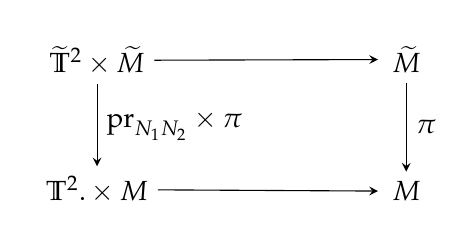
\begin{tikzpicture}
\matrix (m) [matrix of math nodes,row sep=3em,column sep=4em,minimum width=2em]
{
	\widetilde{\T}^2 \times \widetilde{M}  	&  	 & \widetilde{M} \\
	\T^2. \times M 	 & 	 & M   \\};
\path[-stealth]
(m-1-1) edge node [above] {$ \ $} (m-1-3)
(m-1-1) edge node [right] {$\mathrm{pr}_{N_1N_2} \times \pi $} (m-2-1)
(m-1-3) edge node [right] {$\pi$} (m-2-3)
(m-2-1) edge node [above] {$ \ $} (m-2-3);

\end{tikzpicture}


where  $\widetilde{\T}^2 \approx \T^2$.
Let $\widetilde{p} = \left( \widetilde{p}_1, \widetilde{p}_2\right) $ be the generator of the associated with $\widetilde{\T}^2$ two-parameters group $\widetilde{U}\left(s \right) $
so that
\begin{equation*}
\widetilde{U}\left(s \right) = \exp\left( i\left( s_1 \widetilde{p}_1 + s_2 \widetilde{p}_2\right)\right).
\end{equation*}	
The covering $\widetilde{M} \to M$ induces an involutive injective homomorphism
\begin{equation*}
\varphi:\Coo\left(M \right)\to\Coo\left( \widetilde{M} \right).
\end{equation*}


Suppose $M \to M/\T^2$ is submersion, and suppose there is  a weak fibration $\T^2 \to M \to M/\T^2$ (cf. \cite{spanier:at})
There is the exact \textit{homotopy sequence of the weak fibration}
\bean
\dots \to \pi_n\left( \T^2, e_0\right) \xrightarrow{i_{\#}} \pi_n\left( M, e_0\right)  \xrightarrow{p_{\#}} \pi_n\left( M/\T^2, b_0\right) \xrightarrow{\overline\partial} \pi_{n-1}\left( \T^2, e_0\right) \to \dots\\
\dots \to \pi_2\left( M/\T^2, b_0\right) \xrightarrow{\overline\partial} \pi_1\left( \T^2, e_0\right) \xrightarrow{i_{\#}} \pi_1\left( M, e_0\right)  \xrightarrow{p_{\#}} \pi_1\left( M/\T^2, b_0\right) \xrightarrow{\overline\partial} \pi_0\left( \T^2, e_0\right) \to \dots 
\eean
(cf. \cite{spanier:at}) where $\pi_n$ is the $n^{\mathrm{th}}$ homotopical group for any $n\in \N^0$.
If $\pi:\widetilde{M} \to M$ is a finite-fold regular covering then there is the natural surjective homomorphism $
\pi_1\left( M, e_0\right) \to G\left( \left.\widetilde{M}~\right|M\right)$. If $\pi:\widetilde{M} \to M$ induces a covering $\pi:\widetilde{M}/\T^2 \to M / \T^2$  then 
the  homomorphism $
\varphi:\pi_1\left( M, e_0\right) \to G\left( \left.\widetilde{M}~\right|M\right)$ can be included into the following commutative diagram.

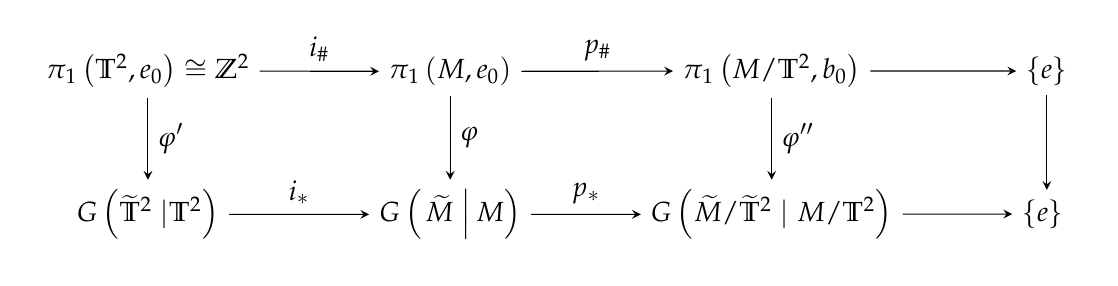
\begin{tikzpicture}
\matrix (m) [matrix of math nodes,row sep=3em,column sep=4em,minimum width=2em]
{
	\pi_1\left(\T^2, e_0 \right)\cong \Z^2 &  \pi_1\left( M, e_0\right) &  \pi_1\left( M/\T^2, b_0\right) &  \{e\} \\
	G\left(\widetilde{\T}^2~|\T^2 \right)  & G\left( \left.\widetilde{M}~\right|M\right) & G\left(\widetilde{M}/\widetilde{\T}^2~|~M/\T^2\right)  & \{e\} \ \\};
\path[-stealth]
(m-1-1)  edge node [right] {$\varphi'$} (m-2-1)
(m-1-2)  edge node [right] {$\varphi$} (m-2-2)
(m-1-3)  edge node [right] {$\varphi''$} (m-2-3)
(m-1-1)  edge node [above] {$i_{\#} $} (m-1-2)
(m-1-2)  edge node [above] {$p_{\#} $} (m-1-3)
(m-2-1)  edge node [above] {$i_*$} (m-2-2)
(m-2-2)  edge node [above] {$p_*$} (m-2-3)
(m-1-3)  edge node [right] {$ $} (m-1-4)
(m-1-4)  edge node [right] {$ $} (m-2-4)
(m-2-3)  edge node [right] {$ $} (m-2-4);
\end{tikzpicture}



Denote by $G \stackrel{\mathrm{def}}{=}G\left( \left.\widetilde{M}~\right|M\right)$, $~G' \stackrel{\mathrm{def}}{=}G\left(\widetilde{\T}^2~|\T^2 \right)$, $~G'' \stackrel{\mathrm{def}}{=}G\left(\widetilde{M}/\widetilde{\T}^2~|~M/\T^2\right)$. From the above construction it turns out that $G' =G\left(\widetilde{\T}^2~|\T^2 \right) = \Z_{N_1} \times \Z_{N_2}$. Otherwise there is an inclusion of Abelian groups $G\left(\widetilde{\T}^2~|\T^2 \right) \subset \widetilde{\T}^2$. The action $\widetilde{\T}^2 \times \widetilde{M} \to  \widetilde{M}$ is free, so the action $G' \times \widetilde{M} \to $ is free, so the natural homomorphism $G' \to G$ is injective, hence there is an exact sequence of groups
\be\label{isospectral_gr_eqn}
\{e\} \to G' \to G \to G'' \to \{e\}.
\ee


Let $\th, \widetilde{\th} \in \R$ be such that
$$
\widetilde{\th}= \frac{\th +  n}{N_1N_2}, \text{ where }n \in \Z.
$$
If $\lambda= e^{2\pi i \th}$, $\widetilde{\lambda}= e^{2\pi i \widetilde{\th}}$ then
$
\lambda = \widetilde{\lambda}^{N_1N_2}.
$
There are isospectral deformations $\Coo\left(M_\th \right), \Coo\left( \widetilde{M}_{\widetilde{\th}} \right)$ and $\C$-linear isomorphisms
$l:\Coo\left(M \right) \to \Coo\left(M_\th \right)$, $\widetilde{l}:\Coo\left( \widetilde{M} \right) \to \Coo\left( \widetilde{M}_{\widetilde{\th}} \right)$.
These isomorphisms and the inclusion $\varphi$ induces the inclusion
\begin{equation*}
\begin{split}
\varphi_\th:\Coo\left(M_\th \right)\to\Coo\left( \widetilde{M}_{\widetilde{\th}} \right),
\\
\varphi_{\widetilde{\th}}\left(\Coo\left(M_\th \right) \right)_{n_1,n_2} \subset \Coo\left( \widetilde{M}_{\widetilde{\th}} \right)_{n_1N_1,~ n_2N_2}.
\end{split}
\end{equation*}
Denote by $G = G\left( \left.\widetilde{M}~\right|M\right)$ the group of covering transformations.   Since $\widetilde{l}$ is a $\C$-linear isomorphism the action of $G$ on $\Coo\left( \widetilde{M} \right)$ induces a $\C$-linear action  $G \times \Coo\left( \widetilde{M}_{ \widetilde{\th}} \right)  \to \Coo\left( \widetilde{M}_{ \widetilde{\th}} \right)$. According to the definition of the action of $\widetilde{\T}^2$ on $\widetilde{M}$ it follows that the action of $G$ commutes with the action of $\widetilde{\T}^2$.
It turns out
$$
g \Coo\left( \widetilde{M} \right)_{n_1,n_2} = \Coo\left( \widetilde{M} \right)_{n_1,n_2}
$$
for any $n_1, n_2 \in \Z$ and $g \in G$.
If $\widetilde{a} \in \Coo\left( \widetilde{M} \right)_{n_1,n_2}$, $\widetilde{b} \in \Coo\left( \widetilde{M} \right)_{n'_1,n'_2}$ then  $g\left( \widetilde{a}\widetilde{b}\right)= \left(g\widetilde{a} \right) \left(g\widetilde{b} \right)\in \Coo\left( \widetilde{M} \right)_{n_1+n'_1,n_2+n'_2} $. One has
\begin{equation*}
	\begin{split}
		\widetilde{l}\left(\widetilde{a}\right)\widetilde{l}\left(\widetilde{b}\right)= \widetilde{\la}^{n'_1n_2}\widetilde{l}\left(\widetilde{a}\widetilde{b}\right), \\
		\widetilde{\la}^{n_2\widetilde{p}_1}l\left( \widetilde{b}\right) = \widetilde{\la}^{n'_1n_2}l\left( \widetilde{b}\right) \widetilde{\la}^{n_2\widetilde{p}_1},\\
		\widetilde{l}\left(g \widetilde{a}\right)\widetilde{l}\left(g \widetilde{b}\right)= g \widetilde{a}\widetilde{\la}^{n_2\widetilde{p}_1}g \widetilde{b}\widetilde{\la}^{n'_2\widetilde{p}_1}= \widetilde{\la}^{n'_1n_2} g\left(\widetilde{a}\widetilde{b} \right) \widetilde{\la}^{\left( n_2+n_2'\right) \widetilde{p}_1}.
	\end{split}
\end{equation*}
On the other hand
\begin{equation*}
	\begin{split}
		g\left( \widetilde{l}\left(\widetilde{a}\right)\widetilde{l}\left(\widetilde{b}\right)\right) = g\left( \widetilde{\la}^{n'_1n_2}\widetilde{l}\left(\widetilde{a}\widetilde{b}\right)\right)= \widetilde{\la}^{n'_1n_2} g\left(\widetilde{a}\widetilde{b} \right) \widetilde{\la}^{\left( n_2+n_2'\right) \widetilde{p}_1}. 
	\end{split}
\end{equation*}
From above equations it turns out
$$
\widetilde{l}\left(g \widetilde{a}\right)\widetilde{l}\left(g \widetilde{b}\right) = g\left( \widetilde{l}\left(\widetilde{a}\right)\widetilde{l}\left(\widetilde{b}\right)\right),
$$
i.e. $g$ corresponds to automorphism of $\Coo\left( \widetilde{M}_{ \widetilde{\th}}\right)$. It turns out that $G$ is the group of automorphisms of $\Coo\left( \widetilde{M}_{ \widetilde{\th}}\right)$. From $\widetilde{a} \in \Coo\left( \widetilde{M}_{ \widetilde{\th}}\right)_{n_1,n_2}$ it follows that $\widetilde{a}^* \in \Coo\left( \widetilde{M}_{ \widetilde{\th}}\right)_{-n_1,-n_2}$. One has
$$
g\left(\left( \widetilde{l}\left(\widetilde{a}\right)\right)^* \right) =  g\left( \widetilde{\la}^{-n_2\widetilde{p_1}}\widetilde{a}^*\right) =
g \left(\widetilde{\la}^{n_1 n_2} \widetilde{a}^*\widetilde{\la}^{-n_2\widetilde{p_1}}\right) = \widetilde{\la}^{n_1 n_2} g\left(\widetilde{l}\left(\widetilde{a}^* \right)  \right). 
$$
On the other hand
$$
\left(g \widetilde{l}\left(\widetilde{a}\right) \right)^*= \left(\left( g \widetilde{a}\right)\widetilde{\la}^{n_2\widetilde{p_1}}  \right)^*=\widetilde{\la}^{-n_2\widetilde{p_1}}\left(ga^* \right) = \widetilde{\la}^{n_1 n_2}\left(ga^* \widetilde{\la}^{-n_2\widetilde{p_1}}\right)= \widetilde{\la}^{n_1 n_2} g\left(\widetilde{l}\left(\widetilde{a}^* \right)  \right),
$$
i.e. $g\left(\left( \widetilde{l}\left(\widetilde{a}\right)\right)^* \right) = \left(g \widetilde{l}\left(\widetilde{a}\right) \right)^*$.
It follows that $g$ corresponds to the involutive automorphism of $\Coo\left( \widetilde{M}_{ \widetilde{\th}}\right)$. Since  $\Coo\left( \widetilde{M}_{ \widetilde{\th}}\right)$ is dense in $C\left( \widetilde{M}_{ \widetilde{\th}}\right)$ there is the unique involutive action $G \times C\left( \widetilde{M}_{ \widetilde{\th}}\right) \to C\left( \widetilde{M}_{ \widetilde{\th}}\right)$.
For any $y_0 \in M/\T^2$ there is a point $x_0 \in M$ mapped onto $y_0$ and a connected submanifold $\mathcal U \subset M$ such that:
\begin{itemize}
	\item $\dim \mathcal U= \dim M-2$,
	\item $\mathcal U$ is transversal to orbits of $\T^2$-action,
	\item The  fibration $\T^2 \to \mathcal U \times \T^2 \to \mathcal U \times \T^2 / \T^2$ is the restriction of the fibration $\T^2 \to M \to M/\T^2$,
	\item The image  $\mathcal V_{y_0} \in M/\T^2$ of $\mathcal U \times \T^2$ in $M/\T^2$ is an open neighborhood of $y_0$,
	\item $\mathcal V_{y_0}$ is evenly covered by  $\widetilde{M}/ \widetilde{\T}^2 \to M / \T^2$.
\end{itemize}
It is clear that
$$
M/\T^2 = \bigcup_{y_0 \in M/\T^2} \mathcal V_{y_0}.
$$
Since $M/\T^2$ is compact there is a finite subset $I \in M/\T^2$ such that
$$
M/\T^2 = \bigcup_{y_0 \in I} \mathcal V_{y_0}.
$$
Above equation will be rewritten as
\be\label{isospectral_p_eqn}
M/\T^2 = \bigcup_{\iota \in I} \mathcal V_{\iota}
\ee
where $\iota$ is just an element of the  finite set $I$ and we denote corresponding transversal submanifold by $\mathcal{U}_\iota$. There is a smooth partition of unity subordinated to \eqref{isospectral_p_eqn}, i.e. there is a set $\left\{a_\iota \in \Coo\left(M /\T^2\right)  \right\}_{\iota \in I}$ of positive elements such that
\be\label{isospectral_part_eqn}
1_{C\left(M /\T^2\right) }= \sum_{\iota \in I} a_\iota~,\\
\ee
\be\nonumber
a_\iota\left(\left( M/\T^2\right)  \setminus \mathcal V_{\iota}\right) = \{0\}.
\ee
Denote by 
\be\label{isospectral_e_eqn}e_\iota \stackrel{\mathrm{def}}{=} \sqrt{a_\iota} \in \Coo\left( M /\T^2\right).
\ee  For any $\iota \in I$ we select an open subset $\widetilde{\mathcal V}_{\iota} \subset \widetilde{M}/\T^2$ which is homeomorphically mapped onto $\mathcal V_{\iota}$.
If $\widetilde{I}= G'' \times  \mathscr A$ then for any $\left(g'', \iota \right) \in \widetilde{I}$ we define
\be\label{isospectral_vgi_eqn}
\begin{split}
	\widetilde{\mathcal V}_{\left(g'', \iota \right)} = g''	\widetilde{\mathcal V}_{\iota}.
\end{split}
\ee
 Similarly we select a transversal submanifold
\be\nonumber%\label{isospectral_u_eqn}
\widetilde{\mathcal U}_{\iota} \subset \widetilde{M}
\ee 
 which is homeomorphially mapped onto $\mathcal U_{\iota}$. For any $\left(g'', \iota \right) \in \widetilde{I}$ we define
 \be\label{isospectral_wgi_eqn}
 \begin{split}
 	\widetilde{\mathcal U}_{\left(g'', \iota \right)} = g	\widetilde{\mathcal U}_{\iota}.
 \end{split}
 \ee
 where $g \in G$ is an arbitrary element mapped to $g''$.
   The set $\mathcal V_{\iota}$ is evenly covered by $\pi'':\widetilde{M}/\widetilde{\T}^2\to M/\T^2$, so one has
\be\label{isostectral_empt_eqn}
g\widetilde{\mathcal V}_{\iota}\bigcap \widetilde{\mathcal V}_{\iota} = \emptyset; \text{ for any nontrivial } g \in G''.
\ee

If $\widetilde{e}_\iota \in \Coo\left(\widetilde M / \widetilde \T^2 \right) $ is given by 
$$
\widetilde{e}_\iota\left(\widetilde{x} \right) = 
\left\{\begin{array}{c l}
e_\iota\left( \pi''\left( \widetilde{x} \right) \right)  & \widetilde{x} \in \widetilde{\mathcal U}_\iota \\
0 & \widetilde{x} \notin \widetilde{\mathcal U}_\iota
\end{array}\right.
$$
then from \eqref{isospectral_part_eqn} and \eqref{isostectral_empt_eqn} it turns out
\begin{equation}
\label{isospectral_partg_eqn}
\begin{split}
1_{C\left(\widetilde M/ \widetilde \T^2 \right) } = \sum_{g \in G''} \sum_{\iota \in I} \widetilde{e}^2_{\iota},\\
\left( g\widetilde{e}_{\iota}\right)\widetilde{e}_{\iota} = 0; \text{ for any nontrivial } g \in G''. 
\end{split}
\end{equation}
If $\widetilde{I}= G'' \times I$ and $\widetilde{e}_{\left(g, \iota\right)} = g \widetilde{e}_{ \iota}$ for any $\left(g, \iota\right)  \in G'' \times I$ then from  \eqref{isospectral_partg_eqn} it turns out
\begin{equation}
\label{isospectral_parti_eqn}
\begin{split}
1_{C\left( \widetilde M / \widetilde \T^2 \right) } =\sum_{\widetilde{\iota} \in \widetilde{I}} \widetilde{e}^2_{\widetilde{\iota}},\\
\left( g\widetilde{e}_{\widetilde{\iota}}\right)\widetilde{e}_{\widetilde{\iota}} = 0; \text{ for any nontrivial } g \in G'',\\
1_{C\left( \widetilde M / \widetilde \T^2 \right) } =  \sum_{\widetilde{\iota} \in \widetilde{I}} \widetilde{e}_{\widetilde{\iota}}\left\rangle \right\langle\widetilde{e}_{\widetilde{\iota}}~.
\end{split}
\end{equation}
It is known that $C\left(\T^2 \right)$ is an universal commutative $C^*$-algebra generated by two unitary elements $u, v$, i.e. there are following relations
\be\label{isospectral_gen_eqn}
\begin{split}
uu^*=u^*u=vv^*=v^*v= 1_{C\left(\T^2 \right)},\\
uv = vu, ~u^*v = vu^*,~uv^*= v^*u, ~ u^*v^*=v^*u^*.
\end{split}
\ee
If $J = I \times \Z \times \Z$ then for any $\left({\iota}, j, k \right) \in J$ there is an element ${f}'_{\left({\iota}, j, k \right)} \in \Coo\left( {\mathcal U}_{{\iota}} \times {\T}^2\right) $ given by
\be\label{isospectral_f's_eqn}
{f}'_{\left({\iota}, j, k \right)} = {e}_{{\iota}} {u}^j{
	v}^k
\ee
where ${e}_{{\iota}}\in \Coo\left( {M}/ {\T}^2\right)$ is regarded as element of $\Coo\left( {M}\right)$.  
Let $p: {M} \to {M} / {\T}^2$.
Denote by ${f}_{\left({\iota}, j, k \right)}\in \Coo\left({M} \right)$ an element given by
\be\label{isospectral_fs_eqn}
\begin{split}
{f}_{\left({\iota}, j, k \right)}\left( {x}\right) =
\left\{\begin{array}{c l}
	{f}'_{\left({\iota}, j, k \right)}\left( {x}\right) & p\left({x} \right)  \in {\mathcal V}_{{\iota}} \\
	0 & p\left( {x}\right)  \notin {\mathcal V}_{{\iota}} 
\end{array}\right.,\\
\text{where the right part of the above equation  assumes the inclusion } \mathcal U_{{\iota}} \times {\T}^2 \hookto M.
\end{split}
\ee 
If we denote by $\widetilde{u}, \widetilde{v} \in U\left( C\left( \widetilde{\T^2} \right) \right)$ unitary generators of $C\left( \widetilde{\T^2} \right)$ then the covering $\pi':\widetilde{\T^2} \to \T^2$ corresponds to a *-homomorphism $C\left(\T^2 \right) \to  C\left( \widetilde{\T^2}\right)$ given by
\bean
u \mapsto \widetilde{u}^{N_1},\\
v \mapsto \widetilde{v}^{N_2}.
\eean
There is the natural action of $G\left( \widetilde{\T}^2~|~{\T^2}\right)\cong \Z_{N_1} \times \Z_{N_2}$ on $C\left(\T^2 \right)$ given by
\be\label{isospectral_uv_eqn}
\begin{split}
\left(\overline{k}_1, \overline{k}_2 \right) \widetilde{u} = e^{\frac{2\pi i k_1}{N_1}}\widetilde{u},\\
\left(\overline{k}_1, \overline{k}_2 \right) \widetilde{v} = e^{\frac{2\pi i k_2}{N_1}}\widetilde{v}
\end{split}
\ee
where $\left(\overline{k}_1, \overline{k}_2 \right) \in \Z_{N_1} \times \Z_{N_2}$. 
If we consider $C\left( \widetilde{\T}^2\right)_{C\left( {\T^2}\right)}$ as a right Hilbert module which corresponds to a finite-fold noncommutative covering then one has
\be\label{isospectral_tor_eqn}
\begin{split}
\left\langle \widetilde{u}^{j'} \widetilde{v}^{k'}, \widetilde{u}^{j''} \widetilde{v}^{k''}  \right\rangle_{C\left( \widetilde{\T^2}\right)} = N_1N_2\delta_{j'j''} \delta_{k'k''}1_{C\left( {\T^2}\right)},\\
1_{C\left( \widetilde{\T^2}\right)}= \frac{1}{N_1N_2}\sum_{\substack{j = 0\\ k = 0}}^{\substack{j = N_1\\ k = N_2}} \widetilde{u}^{j} \widetilde{v}^{k}\left\rangle \right\langle \widetilde{u}^{j} \widetilde{v}^{k}.
\end{split}
\ee
If $\widetilde{J} = \widetilde{I} \times \left\{0, \dots, N_1-1\right\} \times \left\{0, \dots, N_2-1\right\}$ then for any $\left(\widetilde{\iota}, j, k \right) \in \widetilde{J}$ there is an element $\widetilde{f}'_{\left(\widetilde{\iota}, j, k \right)} \in \Coo\left( \widetilde{\mathcal U}_{\widetilde{\iota}} \times \widetilde{\T}^2\right) $ given by
\be\label{isospectral_f'_eqn}
\widetilde{f}'_{\left(\widetilde{\iota}, j, k \right)} = \widetilde{e}_{\widetilde{\iota}} \widetilde{u}^j\widetilde{
v}^k
\ee
where $\widetilde{e}_{\widetilde{\iota}}\in \Coo\left( \widetilde{M}/ \widetilde{\T}^2\right)$ is regarded as element of $\Coo\left( \widetilde{M}\right)$.  
Let $p: \widetilde{M} \to \widetilde{M} / \widetilde{\T}^2$.
Denote by $\widetilde{f}_{\left(\widetilde{\iota}, j, k \right)}\in \Coo\left(\widetilde{M} \right)$ an element given by
\be\label{isospectral_f_eqn}
\begin{split}
\widetilde{f}_{\left(\widetilde{\iota}, j, k \right)}\left( \widetilde{x}\right) =
\left\{\begin{array}{c l}
	\widetilde{f}'_{\left(\widetilde{\iota}, j, k \right)}\left( \widetilde{x}\right) & p\left(\widetilde{x} \right)  \in \widetilde{\mathcal V}_{\widetilde{\iota}} \\
	0 & p\left( \widetilde{x}\right)  \notin \widetilde{\mathcal V}_{\widetilde{\iota}} .
\end{array}\right.\\
\text{where right the part of the above equation assumes the inclusion }  \widetilde{\mathcal U}_{ \widetilde{\iota}} \times  \widetilde{\T}^2 \hookto  \widetilde{M}.
\end{split}
\ee 
Any element $\widetilde{e}_{\widetilde{\iota}} \in C\left(\widetilde{M}/\widetilde{   \T}^2 \right)$ is regarded as element of $C\left(\widetilde{M}\right)$. From $\widetilde{e}_{\widetilde{\iota}} \in \Coo\left(\widetilde{M}\right)_{0,0}$ it turns out $\widetilde{l}\left(\widetilde{e}_{\widetilde{\iota}} \right)  = \widetilde{e}_{\widetilde{\iota}}$,  $~~\left\langle \widetilde{l}\left( \widetilde{e}_{\widetilde{\iota}'}\right) , \widetilde{l}\left( \widetilde{e}_{\widetilde{\iota}''}\right)  \right\rangle_{C\left( \widetilde{M}_{ \widetilde{\th}}\right) } = \left\langle  \widetilde{e}_{\widetilde{\iota}'} ,  \widetilde{e}_{\widetilde{\iota}''}  \right\rangle_{C\left( \widetilde{M}\right) } $.

From \eqref{isospectral_parti_eqn}-\eqref{isospectral_f_eqn} it follows that
\be\label{isospectral_undec_eqn}
1_{C\left(\widetilde{M} \right) }= \frac{1}{N_1N_2}\sum_{\widetilde{\iota} \in \widetilde{I}} \sum_{\substack{j = 0\\ k = 0}}^{\substack{j = N_1-1\\ k = N_2-1}} \widetilde{f}_{\left(\widetilde{\iota}, j, k \right)}\left\rangle \right\langle \widetilde{f}_{\left(\widetilde{\iota}, j, k \right)},
\ee
\be\nonumber%\label{isospectral_fprod_eqn}
\left\langle \widetilde{f}_{\left(\widetilde{\iota}', j', k' \right)}, \widetilde{f}_{\left(\widetilde{\iota}'', j'', k'' \right)} \right\rangle_{C\left( \widetilde{M}\right) } = \frac{1}{N_1N_2} \delta_{j'j''}\delta_{k'k''}\left\langle \widetilde{e}_{\widetilde{\iota}'}, \widetilde{e}_{\widetilde{\iota}''} \right\rangle_{C\left( \widetilde{M}\right) }\in \Coo\left(M \right),
\ee
\be\label{isospectral_fprodl_eqn}
\left\langle \widetilde{l}\left( \widetilde{f}_{\left(\widetilde{\iota}', j', k' \right)}\right) , \widetilde{l}\left( \widetilde{f}_{\left(\widetilde{\iota}'', j'', k'' \right)}\right)  \right\rangle_{C\left( \widetilde{M}_{\widetilde{   \th}}\right) } =\frac{1}{N_1N_2} \delta_{j'j''}\delta_{k'k''}\left\langle \widetilde{e}_{\widetilde{\iota}'}, \widetilde{e}_{\widetilde{\iota}''} \right\rangle_{C\left( \widetilde{M}_{\widetilde{   \th}}\right) }\in  \Coo\left(M_\th \right).
\ee
From the \eqref{isospectral_undec_eqn} it turns out that $C\left(\widetilde{M} \right)$  is a right $C\left(M \right)$ module generated by  finite set of elements $\widetilde{f}_{\left(\widetilde{\iota}, j, k \right)}$ where $\left(\widetilde{\iota}, j, k \right) \in \widetilde{J}$, i.e. any $\widetilde{a} \in C\left(\widetilde{M} \right)$ can be represented as
\be\label{isospectral_wa_eqn}
\widetilde{a} = \sum_{\widetilde{\iota} \in \widetilde{I}} \sum_{\substack{j = 0\\ k = 0}}^{\substack{j = N_1-1\\ k = N_2-1}} \widetilde{f}_{\left(\widetilde{\iota}, j, k \right)} a_{\left(\widetilde{\iota}, j, k \right)}; \text{ where } a_{\left(\widetilde{\iota}, j, k \right)} \in C\left( M\right). 
\ee
Moreover if $\widetilde{a} \in \Coo\left(\widetilde{M} \right)$ then one can select $a_{\left(\widetilde{\iota}, j, k \right)} \in \Coo\left(M \right)$. However any $a_{\left(\widetilde{\iota}, j, k \right)} \in \Coo\left(M \right)$ can be uniquely
written as a doubly infinite
norm convergent sum of homogeneous elements,
\begin{equation*}
a_{\left(\widetilde{\iota}, j, k \right)} = \sum_{n_1,n_2} \, \widehat{T}_{n_1,n_2} \, ,
\end{equation*}

with $\widehat{T}_{n_1,n_2}$ of bidegree $(n_1,n_2)$ and where the sequence
of norms $||
\widehat{T}_{n_1,n_2} ||$ is of
rapid decay in $(n_1,n_2)$. One has
\bea\label{isospectral_sec_eqn}
\widetilde{l}\left(\widetilde{f}_{\left(\widetilde{\iota}, j, k \right)} a_{\left(\widetilde{\iota}, j, k \right)}\right) = \sum_{n_1, n_2}  \widetilde{f}_{\left(\widetilde{\iota}, j, k \right)} \widehat{T}_{n_1,n_2} \widetilde{\lambda}^{\left( N_2n_2+j \right) \widetilde{p}_1}= \sum_{n_1, n_2} \widetilde{f}_{\left(\widetilde{\iota}, j, k \right)} \widetilde{\lambda}^{j \widetilde{p}_1}  \widetilde{\lambda}^{kN_1n_1}\widehat{T}_{n_1,n_2} \widetilde{\lambda}^{N_2n_2 \widetilde{p}_1} 
\eea
%\bea\label{isospectral_sect_eqn}
%\widetilde{l}\left(\widetilde{f}_{\left(\widetilde{\iota}, j, k \right)} a_{\left(\widetilde{\iota}, j, k \right)}\right) = \sum_{n_1, n_2}  \widetilde{f}_{\left(\widetilde{\iota}, j, k \right)} \widehat{T}_{n_1,n_2} \widetilde{\lambda}^{\left( N_2n_2+j \right) \widetilde{p}_1}= \sum_{n_1, n_2} \widetilde{f}_{\left(\widetilde{\iota}, j, k \right)} \widetilde{\lambda}^{j \widetilde{p}_1}  \widetilde{\lambda}^{kN_1n_1}\widehat{T}_{n_1,n_2} \widetilde{\lambda}^{N_2n_2 \widetilde{p}_1} 
%\eea

the sequence
of norms $||
\widetilde{\lambda}^{kN_2n_2}\widehat{T}_{n_1,n_2} ||=||
\widehat{T}_{n_1,n_2} ||$ is of
rapid decay in $(n_1,n_2)$ it follows that
\begin{equation}\label{isospectral_a_eqn}
a'_{\left(\widetilde{\iota}, j, k \right)} = \sum_{n_1,n_2} \, \widetilde{\lambda}^{kN_1n_1} \widehat{T}_{n_1,n_2} \in \Coo\left(M \right) 
\end{equation}
From \eqref{isospectral_wa_eqn} - \eqref{isospectral_a_eqn} it turns out
\be\label{isospectral_sum_eqn}
\widetilde{l}\left( \widetilde{a}\right)  = \sum_{\widetilde{\iota} \in \widetilde{I}} \sum_{\substack{j = 0\\ k = 0}}^{\substack{j = N_1-1\\ k = N_2-1}} \widetilde{l}\left( \widetilde{f}_{\left(\widetilde{\iota}, j, k \right)} \right) l\left( a'_{\left(\widetilde{\iota}, j, k \right)}\right) ; \text{ where } l\left( a'_{\left(\widetilde{\iota}, j, k \right)}\right) \in \Coo\left( M_\th \right).
\ee
However $C\left(\widetilde{M}_{\widetilde{\th}} \right)$ is the norm  completion of $\Coo\left(\widetilde{M}_\th \right)$, so from \eqref{isospectral_sum_eqn} it turns out that  $C\left(\widetilde{M}_{\widetilde{\th}} \right)$ is a right Hilbert $C\left({M}_{{\th}} \right)$-module generated by a finite set
\be\label{isospectral_xi_eqn}
\Xi=\left\{\widetilde{l}\left(\widetilde{f}_{\left(\widetilde{\iota}, j, k \right)} \right) \in   \Coo\left(\widetilde{M}_{\widetilde{\th}} \right)   \right\}_{\left(\widetilde{\iota}, j, k \right) \in \widetilde{J}}
\ee  From the Lemma \ref{fin_hpro_lem} it follows that the module is projective.
So one has the following theorem.
\begin{thm}\label{isospectral_fin_thm}
	The triple $\left( C\left( M_\th\right), C\left( \widetilde{M}_{ \widetilde{\th}}\right), G\left(\widetilde{M}~|~ M \right)\right)   $ is an unital noncommutative finite-fold  covering.
\end{thm}
\subsection{Induced representation}
\paragraph*{}

From \eqref{isospectral_fprodl_eqn} it turns out
\be\label{nt_hilb_eqn}
\begin{split}
\left\langle \widetilde{l}\left(  \widetilde{f}_{\left(\widetilde{\iota}', j', k' \right)}\right) , \widetilde{l}\left(\widetilde{f}_{\left(\widetilde{\iota}'', j'', k'' \right)}\right)  \right\rangle_{C\left(\widetilde{ M}_{\widetilde{\th}}\right) } = \delta_{j'j''}\delta_{k'k''}\left\langle \widetilde{l}\left( \widetilde{e}_{\widetilde{\iota}'}\right) , \widetilde{l}\left( \widetilde{e}_{\widetilde{\iota}''}\right)  \right\rangle_{C\left( \widetilde{M}_{ \widetilde{\th}}\right) }= \\
=  \delta_{j'j''}\delta_{k'k''}\left\langle  \widetilde{e}_{\widetilde{\iota}'}, \widetilde{e}_{\widetilde{\iota}''}\right\rangle_{C\left( \widetilde{M}_{ \widetilde{\th}}\right)}={e}_{\widetilde{\iota}'} {e}_{\widetilde{\iota}''} \in  \Coo\left(M_\th \right).
\end{split}
\ee

Let $g \in G$ be any element, and let $\widetilde{l}\left(\widetilde{f}_{\left(\widetilde{\iota}, j, k \right)}\right)  \in \Xi$ where $\Xi$ is given by \eqref{isospectral_xi_eqn}. From \eqref{isospectral_f'_eqn}  and \eqref{isospectral_f_eqn} it turns out 
\be
\widetilde{l}\left( \widetilde{f}_{\left(\widetilde{\iota}, j, k \right)}\right)  = \widetilde{e}_{\widetilde{\iota}} \widetilde{l}\left( \widetilde{u}^j\widetilde{
	v}^k\right) = \widetilde{e}_{\widetilde{\iota}}  \widetilde{u}^j\widetilde{
	v}^k\widetilde{\la}^{k\widetilde{p}_1}.
\ee
If $g \in G$ be any element, then from the exact sequence \eqref{isospectral_gr_eqn} $\{e\} \to G' \to G \to G'' \to \{e\}$ it follows that there is $g''\in G''$ which is the image of $g$.  For any $\widetilde{\iota}\in \widetilde{I} = G''\times I$ there is $\widetilde{\iota}' \in \widetilde{I}$ such that $g''$ transforms $\widetilde{\iota}$ to  $\widetilde{\iota}~'$. If $\widetilde{\mathcal V}_{\widetilde{\iota}} \in \widetilde{M}/\widetilde{\T}^2$ is given by \eqref{isospectral_vgi_eqn}, and $\widetilde{\mathcal U}_{\widetilde{\iota}}\in \widetilde{M}$ is given by \eqref{isospectral_wgi_eqn} then there is $g' \in G'\cong \Z_{N_1} \times \Z_{N_2}$ such that
\be\nonumber
\begin{split}
g'' \widetilde{\mathcal V}_{\widetilde{\iota}}=\widetilde{\mathcal V}_{\widetilde{\iota}'},\\
g \widetilde{\mathcal U}_{\widetilde{\iota}}= g' \widetilde{\mathcal U}_{\widetilde{\iota}'}. 
\end{split}
\ee
If $g'$ corresponds  to $\left(\overline{k}_1, \overline{k}_2 \right) \in \Z_{N_1} \times \Z_{N_2}$ then from $g''\widetilde{e}_{\widetilde{\iota}} =\widetilde{e}_{\widetilde{\iota}'}$ and \eqref{isospectral_uv_eqn} it turns out
\be\label{isospectral_trans_eqn}
\begin{split}
	g \widetilde{f}_{\left(\widetilde{\iota}, j, k \right)} = g\left( \widetilde{e}_{\widetilde{\iota}}  \widetilde{u}^j\widetilde{
	v}^k\right)= \left( g''\widetilde{e}_{\widetilde{\iota}}\right) \left( g'\left( \widetilde{u}^j\widetilde{
	v}^k\right)\right) =\\= \widetilde{e}_{\widetilde{\iota}'} \left( e^{\frac{2\pi i jk_1}{N_1}}e^{\frac{2\pi i kk_2}{N_1}}\widetilde{u}^j\widetilde{
	v}^k\right)=e^{\frac{2\pi i jk_1}{N_1}}e^{\frac{2\pi i kk_2}{N_1}}\widetilde{f}_{\left(\widetilde{\iota}', j, k \right)}. 
\end{split}
	\ee
Form above equation it follows that for any $\widetilde{\iota}_1, \widetilde{\iota}_2 \in \widetilde{I}$, $~g_1, g_2 \in G$, $~j',j'' = 0,\dots N_1-1$, $~k',k'' = 0,\dots N_2-1$ where are $\widetilde{\iota}'_1, \widetilde{\iota}'_2 \in \widetilde{I}$, $l_1, l_2 \in \Z$ such that
\be\label{isospectral_smooth_eqn}
\begin{split}
\left\langle g_1 \widetilde{f}_{\left(\widetilde{\iota}_1, j', k' \right)} , g_2 \widetilde{f}_{\left(\widetilde{\iota}_2, j'', k'' \right)}  \right\rangle_{C\left( \widetilde{M}\right) } = e^{\frac{2\pi i l_1}{N_1}}e^{\frac{2\pi i l_2}{N_2}} \delta_{j'j''}\delta_{k'k''}\left\langle \widetilde{e}_{\widetilde{\iota}_1'}~,~\widetilde{e}_{\widetilde{\iota}_2'} \right\rangle_{C\left( \widetilde{M}\right) }\in \Coo\left(M \right), \\
\left\langle g_1\left( \widetilde{l}\left(  \widetilde{f}_{\left(\widetilde{\iota}_1, j', k' \right)}\right) \right)  , g_2 \left( \widetilde{l}\left( \widetilde{f}_{\left(\widetilde{\iota}_2, j'', k'' \right)} \right) \right)  \right\rangle_{C\left( \widetilde{M}_{\widetilde{   \th}}\right) } = \\=e^{\frac{2\pi i l_1}{N_1}}e^{\frac{2\pi i l_2}{N_2}} \delta_{j'j''}\delta_{k'k''}\left\langle \widetilde{e}_{\widetilde{\iota}_1'}~,~\widetilde{e}_{\widetilde{\iota}_2'} \right\rangle_{C\left( \widetilde{M}_{\widetilde{   \th}}\right) }\in \Coo\left(M_\th \right). 
\end{split}
\ee
%From the above equation it turns out that for any $g_1, g_2 \in G$ there are $l_1, l_2 $\left(\widetilde{\iota}', j', k' \right)$, $\left(\widetilde{\iota}'', j'', k'' \right)$ there is $\eta \in \R$ such that

From \eqref{isospectral_smooth_eqn} it turns out that the finite set $\widetilde{\Xi}=G\Xi$ satisfies to the condition (a) of the Lemma \ref{smooth_matr_lem}, i.e.
\be\label{isospectral_smooth_fin_eqn}
\left\langle \widetilde{l}\left( \widetilde{f}_{\left(\widetilde{\iota}', j', k' \right)}\right),\widetilde{l}\left( \widetilde{f}_{\left(\widetilde{\iota}'', j'', k'' \right)}\right)  \right\rangle_{C\left( \widetilde{M}_{\widetilde{   \th}}\right) } =  \Coo\left(M_\th \right); ~~ \forall \widetilde{l}\left( \widetilde{f}_{\left(\widetilde{\iota}', j', k' \right)}\right),\widetilde{l}\left( \widetilde{f}_{\left(\widetilde{\iota}'', j'', k'' \right)}\right) \in \widetilde{\Xi}.
\ee

\begin{lemma}\label{isospectral_smooth_lem}
	For any $\widetilde{a} \in C\left(  \widetilde{M}_{ \widetilde{\th}}\right) $ following conditions are equivalent
	\begin{enumerate}
		\item[(a)] $\widetilde{a} \in  \Coo\left(  \widetilde{M}_{ \widetilde{\th}}\right)$,
		\item[(b)] $\left\langle \widetilde{l} \left( \widetilde{f}_{\left(\widetilde{\iota}', j', k' \right)}\right) , \widetilde{a}\widetilde{l}\left( \widetilde{f}_{\left(\widetilde{\iota}'', j'', k'' \right)}\right) \right\rangle_{C\left(  \widetilde{M}_{ \widetilde{\th}}\right)} \in \Coo\left(M_\th \right); ~~\forall \widetilde{l} \left( \widetilde{f}_{\left(\widetilde{\iota}', j', k' \right)}\right) , \widetilde{l} \left( \widetilde{f}_{\left(\widetilde{\iota}'', j'', k'' \right)}\right)  \in \Xi$. 
	\end{enumerate}
\end{lemma} 
\begin{proof} (a)$\Rightarrow$(b) For any $g \in G$ following condition holds  $g\widetilde{l}\left( \widetilde{f}_{\left(\widetilde{\iota}', j', k' \right)}\right) , g\widetilde{l}\left( \widetilde{f}_{\left(\widetilde{\iota}'', j'', k'' \right)}\right) \in \Coo\left(  \widetilde{M}_{ \widetilde{\th}}\right)$, hence
	$$ 
	\left\langle \widetilde{l}\left( \widetilde{f}_{\left(\widetilde{\iota}', j', k' \right)}\right) , \widetilde{a}\widetilde{l}\left( \widetilde{f}_{\left(\widetilde{\iota}'', j'', k'' \right)}\right) \right\rangle_{C\left(  \widetilde{M}_{ \widetilde{\th}}\right)}= \sum_{g\in G}g\left(\widetilde{l}\left( \widetilde{f}^*_{\left(\widetilde{\iota}', j', k' \right)}\right) , \widetilde{a}\widetilde{l}\left( \widetilde{f}_{\left(\widetilde{\iota}'', j'', k'' \right)} \right)\right) \in \Coo\left(  \widetilde{M}_{ \widetilde{\th}}\right). 
	$$
	Since $\left\langle \widetilde{l}\left( \widetilde{f}_{\left(\widetilde{\iota}', j', k' \right)}\right),\widetilde{a}\widetilde{l}\left( \widetilde{f}_{\left(\widetilde{\iota}'', j'', k'' \right)}\right)\right\rangle_{C\left(  \widetilde{M}_{ \widetilde{\th}}\right)}$ is $G$-invariant one has $$\left\langle \widetilde{l}\left( \widetilde{f}_{\left(\widetilde{\iota}', j', k' \right)}\right) ,\widetilde{a}\widetilde{l}\left(  \widetilde{f}_{\left(\widetilde{\iota}'', j'', k'' \right)}\right) \right\rangle_{C\left(  \widetilde{M}_{ \widetilde{\th}}\right)}\in \Coo\left(M \right).$$\\
	(b)$\Rightarrow$(a)
	There is the following equivalence
	$$
	\widetilde{e}_{\widetilde{\iota}} \widetilde{a} 	\widetilde{e}_{\widetilde{\iota}} \in \Coo\left(  \widetilde{M}_{ \widetilde{\th}}\right) \Leftrightarrow  \left\langle 	\widetilde{e}_{\widetilde{\iota}}, \widetilde{a} 	\widetilde{e}_{\widetilde{\iota}} \right\rangle_{C\left(  \widetilde{M}_{ \widetilde{\th}}\right)} \in \Coo\left({M}_{ {\th}}\right).
	$$
	Taking into account $\widetilde{e}_{\widetilde{\iota}} = \widetilde{l}\left(\widetilde{f}_{\left(\widetilde{\iota}, 0, 0 \right)} \right) $ one has a following logical equation
\bean
\forall\widetilde{\iota} \in \widetilde{I}~~	\left\langle 	\widetilde{l}\left(\widetilde{f}_{\left(\widetilde{\iota}, 0, 0 \right)}\right) , \widetilde{a} 	\widetilde{l}\left(\widetilde{f}_{\left(\widetilde{\iota}, 0, 0 \right)}\right)  \right\rangle_{C\left(  \widetilde{M}_{ \widetilde{\th}}\right)} \in \Coo\left({M}_{ {\th}}\right) \Leftrightarrow \\ \Leftrightarrow \widetilde{l}\left(\widetilde{f}_{\left(\widetilde{\iota}, 0, 0 \right)}\right)  \widetilde{a} 	\widetilde{l}\left(\widetilde{f}_{\left(\widetilde{\iota}, 0, 0 \right)}\right) \in \Coo\left(  \widetilde{M}_{ \widetilde{\th}}\right)\Rightarrow  \\ \Rightarrow
\widetilde{a} = \sum_{\widetilde{\iota} \in \widetilde{I}} 	\widetilde{e}_{\widetilde{\iota}}	\widetilde{a}	\widetilde{e}_{\widetilde{\iota}} = \sum_{\widetilde{\iota} \in \widetilde{I}} 	\widetilde{l}\left(\widetilde{f}_{\left(\widetilde{\iota}, 0, 0 \right)}\right) 	\widetilde{a}\widetilde{l}\left(\widetilde{f}_{\left(\widetilde{\iota}, 0, 0 \right)}\right) \in \Coo\left(  \widetilde{M}_{ \widetilde{\th}}\right).
\eean
	
%	If $\widetilde{a} \in C\left(  \widetilde{M}_{ \widetilde{\th}}\right)$ then there is the following $C^*$-norm limit $\widetilde{a} = \lim_{m \to \infty} \widetilde{l}\widetilde{b}_m$ where $\widetilde{b}_m \in \Coo\left( \widetilde{M}\right)$. Denote by $\left\|\cdot \right\|_s$ are seminorms given by  \eqref{s_semi_eqn}. If the sequence $\left\{\widetilde{b}_m\right\}$ is not convergent to an element of $\Coo\left( \widetilde{M}\right)$ then there is $s \in \N$ such that
%	$$
%	\sup_{m \in N} \left\|\widetilde{b}_m \right\|_s= \infty.
%	$$
%	The space $\widetilde{M}$ is compact, so there is a convergent sequence $\left\{\widetilde{x}_m \in \widetilde{M}\right\}_{m \in \N}$ such that $\lim_{m \to \infty}  \left\|\widetilde{b}_m \right\|_s\left( \widetilde{x}_m\right) = \infty$. If  $\widetilde{x}=\lim_{m \to \infty} \widetilde{x}_m$ and $\widetilde{\iota} \in \widetilde{I}$ such that $\widetilde{e}_{\widetilde{\iota}} \neq 0$ then 	
%	is a positive $r > 0$ and an open  neighborhood of $\widetilde{\mathcal U}$ of $\widetilde{x}$ such that $\left\|\widetilde{e}_{\widetilde{\iota}} \right\|_s\left( \widetilde{x}'\right)> r$ for any $\widetilde{x}'\widetilde{\mathcal U}$. It turns out
%	$$
%	\lim_{m\to \infty} \left\|\widetilde{e}_{\widetilde{\iota}} \widetilde{b}_m\widetilde{e}_{\widetilde{\iota}}\right\|_s\left( \widetilde{x}_m\right)  = \infty,
%	$$
%hence the sequence $\widetilde{e}_{\widetilde{\iota}} \left\{c_m =\widetilde{b}_m\widetilde{e}_{\widetilde{\iota}}\right\}$ does not convergent to element of $\Coo\left( \widetilde{M}\right)$. However $\widetilde{e}_{\widetilde{\iota}} = \widetilde{f}_{\left( \widetilde{\iota},0,0\right) }$ it follows that
%$$
%\widetilde{f}_{\left( \widetilde{\iota},0,0\right) }\widetilde{a}\widetilde{f}_{\left( \widetilde{\iota},0,0\right) }= \lim_{m \to \infty} \widetilde{l}\left(c_m \right)  \notin \Coo\left( \widetilde{M}\right) .
%$$
%It turns out
%$$
%\left\langle \widetilde{f}_{\left(\widetilde{\iota}, 0,0 \right)}, \widetilde{a}\widetilde{f}_{\left(\widetilde{\iota}, 0, 0 \right)}\right\rangle_{C\left(  \widetilde{M}_{ \widetilde{\th}}\right)} \in \Coo\left(M_\th \right) \notin\Coo\left(M \right).
%$$	
 \end{proof}
\begin{corollary}\label{isospectral_cor}
	Following conditions hold:
	\begin{itemize}
		\item $C\left(\widetilde{M}_{\widetilde{\th}} \right) \bigcap \mathbb{M}_n\left(\Coo\left(M_\th\right) \right) = \Coo\left(\widetilde{M}_{\widetilde{\th}} \right)$,
		\item The unital noncommutative finite-fold covering  $$\left( C\left( M_\th\right), C\left( \widetilde{M}_{ \widetilde{\th}}\right), G\left(\widetilde{M}~|~ M \right)\right)$$ is {smoothly invariant}.
	\end{itemize}
\end{corollary}
\begin{proof}
	Follows from \eqref{isospectral_smooth_fin_eqn}, and Lemmas \ref{smooth_matr_lem}, \ref{isospectral_smooth_lem}.
\end{proof}

From \eqref{isospectral_undec_eqn} for any $\widetilde{a} \in C\left( \widetilde{M}_{ \widetilde{\th}}\right)$ following condition holds
\be\label{isospectral_d_eqn}
\widetilde{a} = \frac{1}{N_1N_2}\sum_{\widetilde{\iota} \in \widetilde{I}} \sum_{\substack{j = 0\\ k = 0}}^{\substack{j = N_1-1\\ k = N_2-1}} \widetilde{l}\left( \widetilde{f}_{\left(\widetilde{\iota}, j, k \right)}\right) \left\langle \widetilde{a},\widetilde{l} \left( \widetilde{f}_{\left(\widetilde{\iota}, j, k \right)}\right) \right\rangle_{C\left( \widetilde{M}_{ \widetilde{\th}}\right)}= \sum_{\widetilde{\iota} \in \widetilde{I}} \sum_{\substack{j = 0\\ k = 0}}^{\substack{j = N_1-1\\ k = N_2-1}} \widetilde{l}\left( \widetilde{f}_{\left(\widetilde{\iota}, j, k \right)}\right)a_{\left(\widetilde{\iota}, j, k \right)}
\ee
where $a_{\left(\widetilde{\iota}, j, k \right)}=\frac{1}{N_1N_2}\left\langle \widetilde{a},\widetilde{l} \left( \widetilde{f}_{\left(\widetilde{\iota}, j, k \right)}\right) \right\rangle_{C\left( \widetilde{M}_{ \widetilde{\th}}\right)}\in C\left( {M}_{ {\th}}\right)$. If $\xi \in L^2\left(M, S \right)$ then
\be\label{isospectral_decomp_eqn}
\begin{split}
\widetilde{a} \otimes \xi = \sum_{\widetilde{\iota} \in \widetilde{I}}~~ \sum_{\substack{j = 0\\ k = 0}}^{\substack{j = N_1-1\\ k = N_2-1}} \widetilde{l}\left( \widetilde{f}_{\left(\widetilde{\iota}, j, k \right)}\right)a_{\left(\widetilde{\iota}, j, k \right)}\otimes \xi = \sum_{\widetilde{\iota} \in \widetilde{I}}~~ \sum_{\substack{j = 0\\ k = 0}}^{\substack{j = N_1-1\\ k = N_2-1}} \widetilde{l}\left( \widetilde{f}_{\left(\widetilde{\iota}, j, k \right)}\right)\otimes a_{\left(\widetilde{\iota}, j, k \right)} \xi=\\
= \sum_{\widetilde{\iota} \in \widetilde{I}} ~~\sum_{\substack{j = 0\\ k = 0}}^{\substack{j = N_1-1\\ k = N_2-1}} \widetilde{l}\left( \widetilde{f}_{\left(\widetilde{\iota}, j, k \right)}\right)\otimes \xi_{\left(\widetilde{\iota}, j, k \right)} \in C\left( \widetilde{M}_{ \widetilde{\th}}\right) \otimes_{C\left( {M}_{ {\th}}\right)} L^2\left(M, S \right),\\ \text{ where } \xi_{\left(\widetilde{\iota}, j, k \right)} = a_{\left(\widetilde{\iota}, j, k \right)}\xi \in   L^2\left(M, S \right).
\end{split}
\ee
Denote by $ \widetilde{\H}=C\left( \widetilde{M}_{ \widetilde{\th}}\right) \otimes_{C\left( {M}_{ {\th}}\right)} L^2\left(M, S \right)$ and let $\left(\cdot, \cdot \right)_{\widetilde{\H}}$ is the given by \eqref{induced_prod_equ} Hilbert product. If $\xi, \eta \in L^2\left(M, S \right)$ then from \eqref{nt_hilb_eqn} it turns out
\be\label{isospectral_hilb_p_eqn}
\left(\widetilde{l} \left( \widetilde{f}_{\left(\widetilde{\iota}', j', k' \right)}\right)  \otimes \xi, ~\widetilde{l} \left( \widetilde{f}_{\left(\widetilde{\iota}'', j'', k'' \right)}\right)  \otimes \eta \right)_{\widetilde{\H}}= N_1N_2\delta_{j'j''}\delta_{k'k''}\left(\xi,{e}_{\widetilde{\iota}'} {e}_{\widetilde{\iota}''} \eta  \right)_{ L^2\left(M, S \right)}.
\ee
From \eqref{isospectral_hilb_p_eqn} it turns out the orthogonal decomposition
\bean
\widetilde{\H} = \bigoplus_{\substack{j = 0\\ k = 0}}^{\substack{j = N_1-1\\ k = N_2-1}}\widetilde{\H}_{jk}~, ~~ \\ \text{ where } \widetilde{\H}_{jk}=\left\{\widetilde{\xi} \in \widetilde{\H}~|~\widetilde{\xi}= \sum_{\widetilde{\iota} \in \widetilde{I}}\widetilde{l}\left( \widetilde{f}_{\left(\widetilde{\iota}, j, k \right)}\right)\otimes \xi_{\left(\widetilde{\iota}, j, k \right)}\in C\left( \widetilde{M}_{ \widetilde{\th}}\right) \otimes_{C\left( {M}_{ {\th}}\right)} L^2\left(M, S \right) \right\}.
\eean
From \eqref{isospectral_hilb_p_eqn} it turns out than for any $0\le j',j''<N_1$ and $0\le k',k''<N_2$ there is an isomorphism of Hilbert spaces given by
\be\label{isospectral_hilb_iso_eqn}
\begin{split}
\Phi^{j'k'}_{j''k''}:\widetilde{\H}_{j'k'}\xrightarrow{\approx}\widetilde{\H}_{j''k''},\\
\widetilde{l} \left( \widetilde{f}_{\left(\widetilde{\iota}, j', k' \right)}\right)  \otimes \xi \mapsto \widetilde{l} \left( \widetilde{f}_{\left(\widetilde{\iota}, j'', k'' \right)}\right)  \otimes \xi.
\end{split}
\ee
Similarly if  $\widetilde{\H}^{\mathrm{comm}}=C\left( \widetilde{M}\right) \otimes_{C\left( {M}\right)} L^2\left(M, S \right)$ then there is the decomposition
\bean
\widetilde{\H}^{\mathrm{comm}} = \bigoplus_{\substack{j = 0\\ k = 0}}^{\substack{j = N_1-1\\ k = N_2-1}}\widetilde{\H}^{\mathrm{comm}}_{jk}~, ~~ \\ \text{ where } \widetilde{\H}^{\mathrm{comm}}_{jk}=\left\{\widetilde{\xi} \in \widetilde{\H}^{\mathrm{comm}}~|~\widetilde{\xi}= \sum_{\widetilde{\iota} \in \widetilde{I}} \widetilde{f}_{\left(\widetilde{\iota}, j, k \right)}\otimes \xi_{\left(\widetilde{\iota}, j, k \right)}\in C\left( \widetilde{M}\right) \otimes_{C\left( {M}\right)} L^2\left(M, S \right) \right\}.
\eean
From the Lemma \eqref{comm_ind_lem} it turns out $\widetilde{\H}^{\mathrm{comm}} = L^2\left( \widetilde{M},\widetilde{S}\right)$ the induced representation is given by the natural action of $C\left( {M}\right)$ on $L^2\left( \widetilde{M},\widetilde{S}\right)$. 
Similarly to \eqref{isospectral_hilb_iso_eqn} for any $0\le j',j''<N_1$ and $0\le k',k''<N_2$ there is an isomorphism of Hilbert spaces given by
\be\label{isospectral_hilb_iso_comm_eqn}
\begin{split}
	\Psi^{j'k'}_{j''k''}:\widetilde{\H}^{\mathrm{comm}}_{j'k'}\xrightarrow{\approx}\widetilde{\H}^{\mathrm{comm}}_{j''k''},\\
 \widetilde{f}_{\left(\widetilde{\iota}, j', k' \right)}  \otimes \xi \mapsto   \widetilde{f}_{\left(\widetilde{\iota}, j'', k'' \right)}  \otimes \xi.
\end{split}
\ee
From $\widetilde{l}\left( \widetilde{f}_{\left(\widetilde{\iota}, 0, 0 \right)}\right)= \widetilde{f}_{\left(\widetilde{\iota}, 0, 0 \right)}=\widetilde{e}_{\widetilde{\iota}}$ it turns out the natural ismomorphism  
\be\label{isospectral_nat_eqn}
\widetilde{\H}^{\mathrm{comm}}_{0,0} \cong \widetilde{\H}_{0,0}
\ee
We would like to define the isomorphism $\varphi:\widetilde{\H} \approx C\left( \widetilde{M}_{ \widetilde{\th}}\right) \otimes_{C\left( {M}_{ {\th}}\right)} L^2\left(M, S \right) \xrightarrow{\approx}\widetilde{\H}^{\mathrm{comm}}$ such that for any $\widetilde{a} \in C\left(\widetilde{M}_{\widetilde{\th}} \right)$, and $\xi \in L^2\left(M,S \right)$ following condition holds 
\be\label{isospectral_varphi_eqn}
\varphi\left( \widetilde{a}\otimes \xi \right)= \widetilde{a}\left(1_{C\left( M\right) } \otimes \xi \right) 
\ee
where the right part of the above equation assumes the action of $C\left(\widetilde{M}_{\widetilde{\th}} \right)$ on $L^2\left( \widetilde{M},\widetilde{S}\right)$ by operators  \eqref{l_defn}. From the decomposition \eqref{isospectral_d_eqn} it turns the equation  \eqref{isospectral_varphi_eqn} is true if and only if it is true for any $\widetilde{a} = \widetilde{l}\left( \widetilde{f}_{\left(\widetilde{\iota}, j, k \right)}\right) a$  where $a \in C\left( {M}_{ \th}\right)$, i.e.
$$
\varphi\left( \widetilde{l}\left( \widetilde{f}_{\left(\widetilde{\iota}, j, k \right)}\right) a\otimes \xi \right)= \widetilde{l}\left( \widetilde{f}_{\left(\widetilde{\iota}, j, k \right)}\right) a\left(1_{C\left( M\right) } \otimes \xi \right),
$$
or equivalently
\be\label{isospectral_varphi_p_eqn}
\varphi\left( \widetilde{l}\left( \widetilde{f}_{\left(\widetilde{\iota}, j, k \right)}\right) \otimes a\xi \right)= \widetilde{l}\left( \widetilde{f}_{\left(\widetilde{\iota}, j, k \right)}\right) \left(1_{C\left( M\right) } \otimes a\xi \right)
\ee
From \eqref{isospectral_hilb_iso_comm_eqn} the right part of \eqref{isospectral_varphi_p_eqn} is given by
$$
\widetilde{l}\left( \widetilde{f}_{\left(\widetilde{\iota}, j, k \right)}\right) \left(1_{C\left( M\right) } \otimes a\xi \right)= \Psi^{0,0}_{jk}\left(\widetilde{\la}^{kp_1} \left(\widetilde{f}_{\left(\widetilde{\iota}, 0, 0\right)} \otimes a\xi \right) \right) 
$$
From the above equation it turns out that if $\eta \in \widetilde{\H}_{j,k}$ then
\be\label{isospectral_jk_p_eqn}
\varphi\left( \eta\right)=\varphi|_{\widetilde{\H}_{j,k}}\left( \eta\right)=  \Psi^{0,0}_{jk}\left( \widetilde{\la}^{kp_1}\Phi^{jk}_{0,0} \left(\eta \right) \right) 
\ee
and 
\bean
\varphi = \bigoplus_{\substack{j = 0\\ k = 0}}^{\substack{j = N_1-1\\ k = N_2-1}} \varphi_{\widetilde{\H}_{j,k}}:\widetilde{\H}\xrightarrow{\approx} \widetilde{\H}^{\mathrm{comm}}
\eean
then from above construction it turns out that $\varphi$ satisfies to \eqref{isospectral_varphi_eqn}. In result we have the following lemma.
\begin{lemma}
	If $\widetilde{\rho}:C\left( \widetilde{M}_{ \widetilde{\th}}\right)\to B\left(\widetilde{\H} \right) $ is induced by $\left(\rho, \left( C\left( M_\th\right), C\left( \widetilde{M}_{ \widetilde{\th}}\right), G\left(\widetilde{M}, M \right)\right)\right)$ then $\widetilde{\rho}$ can be represented by action of $C\left( \widetilde{M}_{ \widetilde{\th}}\right)$ on $ L^2\left( \widetilde{M},\widetilde{S}\right)$ by operators \eqref{l_defn}.
\end{lemma}
\subsection{Coverings of spectral triples}
\paragraph*{}
If ${f}_{\left({\iota}, j, k \right)} \in \Coo \left(M \right)$ is given by \eqref{isospectral_fs_eqn} then from then from \eqref{isospectral_f's_eqn} it turns out 
\be\nonumber
{f}'_{\left({\iota}, j, k \right)} = {e}_{{\iota}} {u}^j{
	v}^k \in C_0\left({\mathcal{U}}_{\iota} \right)= C_0\left({\mathcal{V}}_{\iota} \times \T^2 \right)
\ee
In the above formula the product ${u}^j{
	v}^k$ can be regarded as element of both $C\left( \T^2\right)$ and  $C_b\left({\mathcal{V}}_{\iota} \times \T^2 \right) =  C_b\left({\mathcal{W}}_{\iota} \right)$, where $\mathcal{W}_{\iota}\subset M$ is the homeomorphic image of ${\mathcal{V}}_{\iota} \times \T^2$. Since the Dirac operator $\slashed D$ is invariant with respect to transformations 
$
u \mapsto e^{i\varphi_u}u, ~~ v \mapsto e^{i\varphi_v}v
$
one has
\be\label{isospectral_jdb_eqn}
\left[\slashed D, u \right]= d^{\iota}_uu,~~ \left[\slashed D, v \right]= d^{\iota}_vv
\ee
where $d^\iota_u, d^\iota_v: \mathcal V_\iota \to \mathbb{M}_{\dim S} \left(\C \right)$ are continuous matrix-valued functions. I would like to avoid functions in $C_b\left({\mathcal{U}}_{\iota} \right)$, so instead \eqref{isospectral_jdb_eqn} the following evident consequence of it will be used
\be\label{isospectral_jde_eqn}
\left[\slashed D,a u^jv^k \right]= \left[\slashed D,a \right] u^jv^k  + a\left( jd^\iota_u+kd^\iota_v\right) u^jv^k; ~~ a \in C_0\left( M/ \T^2\right), ~~ \supp a \subset \mathcal{V}_{\iota}.
\ee
In contrary to \eqref{isospectral_jdb_eqn} the equation \eqref{isospectral_jde_eqn} does not operate with $C_b\left({\mathcal{U}}_{\iota} \right)$, it operates with $C_0\left({\mathcal{U}}_{\iota} \right)$. Let $\pi: \widetilde M \to M$ and let $\widetilde{\slashed D} = p^{-1} \slashed D$ be the $\pi$-inverses image of $\slashed D$ (cf. Definition  \ref{top_smooth_inv_im_defn}). Suppose $\widetilde{  \mathcal V}_{\widetilde{\iota}} \subset \widetilde{M}/\widetilde{   \T}^2$ is mapped onto ${  \mathcal V}_{{\iota}} \subset {M}/{   \T}^2$. Then we set $d^{\widetilde{\iota}}_u \stackrel{\mathrm{def}}{=} d^{{\iota}}_u$, $d^{\widetilde{\iota}}_v \stackrel{\mathrm{def}}{=} d^{{\iota}}_v$. The covering $\pi$ maps $\widetilde{\mathcal{V}}_{ \widetilde\iota} \times \widetilde{\T}^2$ onto ${\mathcal{V}}_{\iota} \times \T^2$. If $\widetilde{u}, \widetilde{v} \in C\left(\widetilde{\T}^2 \right)$ are natural generators, then the covering $\widetilde{\T}^2 \to \T^2$ is given by
\bean
C\left(\T^2 \right) \to C\left(\widetilde{\T}^2 \right),\\
u \mapsto \widetilde{u}^{N_1},~~v \mapsto \widetilde{v}^{N_2}.
\eean 
From the above equation and taking into account \eqref{isospectral_jdb_eqn} one has
\be\label{isospectral_du_eqn}
\begin{split}
\left[\widetilde{\slashed D}, \widetilde{u} \right]= \frac{d^{\widetilde{\iota}}_u}{N_1}\widetilde{u},~~ \left[\widetilde{\slashed D}, \widetilde{v} \right]= \frac{d^{\widetilde{\iota}}_v}{N_2}\widetilde{v},\\
\left[\widetilde{\slashed D}, \widetilde{a} \widetilde{u}^j\widetilde{v}^k \right]=\left[\widetilde{\slashed D},\widetilde{a} \right] \widetilde{u}^j\widetilde{v}^k  + \widetilde{a} \left(\frac{j^{\widetilde{\iota}}_u}{N_1} +\frac{k^{\widetilde{\iota}}_v}{N_2}\right) \widetilde{u}^j\widetilde{v}^k;\\ ~~ \widetilde{a} \in C_0\left( \widetilde{M}/ \widetilde{\T}^2\right), ~~ \supp \widetilde{a} \subset \widetilde{\mathcal{V}}_{\widetilde{\iota}}.
\end{split}
\ee
For any $\widetilde{a}\in \Coo\left( \widetilde{M}\right) $ such that $\supp \widetilde{a} \subset  \widetilde{\mathcal{W}}_{\widetilde{\iota}}$ following condition holds
\be\label{isospectral_da_eqn}
\left[\widetilde{\slashed D}, \widetilde{a} \right]= \mathfrak{lift}_{\widetilde{\mathcal{W}}_{\widetilde{\iota}}}\left(\left[{\slashed D}, \mathfrak{desc}\left( \widetilde{a}\right)  \right] \right) 
\ee
If $b \in \Coo\left(M/\T^2 \right)\subset \Coo\left(M \right)$ then from \eqref{isospectral_du_eqn} and \eqref{isospectral_da_eqn} it turns out
\be\nonumber
\begin{split}
\left[\widetilde{\slashed D},  \widetilde{f}_{\left(\widetilde{\iota}, j, k \right)}b u^{j'}v^{k'}\right]   = \sqrt{\widetilde{e}_{\widetilde{\iota}}}\widetilde{u}^j\widetilde{v}^k  u^{j'}v^{k'}\otimes \left[ \slashed D, \sqrt{{e}_{\widetilde{\iota}}} b  \right]+ \\ +  b\sqrt{\widetilde{e}_{\widetilde{\iota}}}\widetilde{u}^j\widetilde{v}^k  u^{j'}v^{k'}\otimes \left[ \slashed D, \sqrt{{e}_{\widetilde{\iota}}}\right]+\\+b
	\sqrt{\widetilde{e}_{\widetilde{\iota}}}\widetilde{u}^j\widetilde{v}^k  u^{j'}v^{k'}\otimes  \sqrt{{e}_{\widetilde{\iota}}}\left(j'd_u+\frac{ jd_u}{N_1} +k'd_v + \frac{kd_v}{N_2}\right)\\
\end{split}
\ee 
and taking into account $\left[ \widetilde{\slashed D}, \widetilde{l}\right]=0$ one has
\be\label{isospectral_predu_eqn}
\begin{split}
	\left[\widetilde{\slashed D}, \widetilde{l}\left(  \widetilde{f}_{\left(\widetilde{\iota}, j, k \right)}b u^{j'}v^{k'}\right) \right]   = \sqrt{\widetilde{e}_{\widetilde{\iota}}}\widetilde{l}\left(\widetilde{u}^j\widetilde{v}^k  u^{j'}v^{k'}\right)\otimes \left[ \slashed D, \sqrt{{e}_{\widetilde{\iota}}} b  \right]+ \\ +  b\sqrt{\widetilde{e}_{\widetilde{\iota}}}\widetilde{l}\left(\widetilde{u}^j\widetilde{v}^k  u^{j'}v^{k'}\right)\otimes \left[ \slashed D, \sqrt{{e}_{\widetilde{\iota}}}\right]+\\+b
	\sqrt{\widetilde{e}_{\widetilde{\iota}}}\widetilde{l}\left(\widetilde{u}^j\widetilde{v}^k  u^{j'}v^{k'}\right)\otimes  \sqrt{{e}_{\widetilde{\iota}}}\left(j'd_u+\frac{ jd_u}{N_1} +k'd_v + \frac{kd_v}{N_2}\right)\\
\end{split}
\ee
Taking into account that  
$
\widetilde{l}\left(\widetilde{u}^j\widetilde{v}^k \right)\widetilde{l}\left( u^{j'}v^{k'}\right)= \widetilde{\la}^{j'N_2k} \widetilde{l}\left(\widetilde{u}^j\widetilde{v}^k  u^{j'}v^{k'}\right)
$ the equation \eqref{isospectral_predu_eqn} is equivalent to


\be\label{isospectral_pred_eqn}
\begin{split}
	\left[\widetilde{\slashed D},  \widetilde{l}\left( \widetilde{f}_{\left(\widetilde{\iota}, j, k \right)}\right) b \widetilde{l}\left( u^{j'}v^{k'}\right) \right]   = \sqrt{\widetilde{e}_{\widetilde{\iota}}}\widetilde{l}\left(\widetilde{u}^j\widetilde{v}^k \right)\widetilde{l}\left( u^{j'}v^{k'}\right)\otimes \left[ \slashed D, \sqrt{{e}_{\widetilde{\iota}}} b  \right]+ \\ +  b\sqrt{\widetilde{e}_{\widetilde{\iota}}}\widetilde{l}\left(\widetilde{u}^j\widetilde{v}^k \right) \widetilde{l}\left( u^{j'}v^{k'}\right)\otimes \left[ \slashed D, \sqrt{{e}_{\widetilde{\iota}}}\right]+\\+b
	\sqrt{\widetilde{e}_{\widetilde{\iota}}}\widetilde{l}\left(\widetilde{u}^j\widetilde{v}^k \right) \widetilde{l}\left( u^{j'}v^{k'}\right)\otimes  \sqrt{{e}_{\widetilde{\iota}}}\left(j'd_u+\frac{ jd_u}{N_1} +k'd_v + \frac{kd_v}{N_2}\right)\\
\end{split}
\ee


For any $\widetilde{a} \in C\left( \widetilde{M}_{ \widetilde{\th}}\right)$ there is the decomposition given by \eqref{isospectral_d_eqn}, i.e.
\be\nonumber 
\widetilde{a} = \sum_{\widetilde{\iota} \in \widetilde{I}} \sum_{\substack{j = 0\\ k = 0}}^{\substack{j = N_1-1\\ k = N_2-1}} \widetilde{l}\left( \widetilde{f}_{\left(\widetilde{\iota}, j, k \right)}\right)a_{\left(\widetilde{\iota}, j, k \right)}
\ee
Let $\Om^1_{\slashed D}$ be the {module of differential forms associated} with the spectral triple  $\left(\Coo\left(M_\th \right) , L^2\left(M,S \right) , \slashed D\right)$ (cf. Definition \ref{ass_cycle_defn}). Let us define a $\C$-linear map
\be\label{isospectral_conn_eqn}
\begin{split}
\nabla: \Coo\left(\widetilde{M}_{\widetilde{\th}} \right) \to \Coo\left(\widetilde{M}_{\widetilde{\th}} \right) \otimes_{\Coo\left(M_\th \right)}\Om^1_{\slashed D}~,\\
\sum_{\widetilde{\iota} \in \widetilde{I}}~~  \sum_{\substack{j = 0\\ k = 0}}^{\substack{j = N_1-1\\ k = N_2-1}} \widetilde{l}\left( \widetilde{f}_{\left(\widetilde{\iota}, j, k \right)}\right)a_{\left(\widetilde{\iota}, j, k \right)}\mapsto \sum_{\widetilde{\iota} \in \widetilde{I}}~~  \sum_{\substack{j = 0\\ k = 0}}^{\substack{j = N_1-1\\ k = N_2-1}} \sqrt{\widetilde{e}_{\widetilde{\iota}}}\widetilde{l}\left(\widetilde{u}^j\widetilde{v}^k \right)\otimes \left[ \slashed D, \sqrt{{e}_{\widetilde{\iota}}} a_{\left(\widetilde{\iota}, j, k \right)}\right]+ \\ + \sum_{\widetilde{\iota} \in \widetilde{I}}~~  \sum_{\substack{j = 0\\ k = 0}}^{\substack{j = N_1-1\\ k = N_2-1}} \sqrt{\widetilde{e}_{\widetilde{\iota}}}\widetilde{l}\left(\widetilde{u}^j\widetilde{v}^k \right) a_{\left(\widetilde{\iota}, j, k \right)}\otimes \left[ \slashed D, \sqrt{{e}_{\widetilde{\iota}}}\right]+\\+
 \sum_{\widetilde{\iota} \in \widetilde{I}}~~  \sum_{\substack{j = 0\\ k = 0}}^{\substack{j = N_1-1\\ k = N_2-1}}\sqrt{\widetilde{e}_{\widetilde{\iota}}}\widetilde{l}\left(\widetilde{u}^j\widetilde{v}^k \right) a_{\left(\widetilde{\iota}, j, k \right)}\otimes  \sqrt{{e}_{\widetilde{\iota}}}\left(\frac{jd_u}{N_1} +\frac{kd_v}{N_2}\right). 
\end{split}
\ee
For any $a \in \Coo\left( M_\th\right)$ following condition holds 
\be\label{isospectral_conn_p_eqn}
\begin{split}
\nabla\left(  \widetilde{l}\left( \widetilde{f}_{\left(\widetilde{\iota}, j, k \right)}\right)a_{\left(\widetilde{\iota}, j, k \right)}a\right) =  \sqrt{\widetilde{e}_{\widetilde{\iota}}}\widetilde{l}\left(\widetilde{u}^j\widetilde{v}^k \right)\otimes \left[ \slashed D, \sqrt{{e}_{\widetilde{\iota}}} a_{\left(\widetilde{\iota}, j, k \right)}a\right]+ \\+ \sqrt{\widetilde{e}_{\widetilde{\iota}}}\widetilde{l}\left(\widetilde{u}^j\widetilde{v}^k \right) a_{\left(\widetilde{\iota}, j, k \right)}a\otimes \left[ \slashed D, \sqrt{{e}_{\widetilde{\iota}}}\right]+
\sqrt{\widetilde{e}_{\widetilde{\iota}}}\widetilde{l}\left(\widetilde{u}^j\widetilde{v}^k \right) a_{\left(\widetilde{\iota}, j, k \right)}a\otimes  \sqrt{{e}_{\widetilde{\iota}}}\left(\frac{jd_u}{N_1} +\frac{kd_v}{N_2}\right)=\\=
 \sqrt{\widetilde{e}_{\widetilde{\iota}}}\widetilde{l}\left(\widetilde{u}^j\widetilde{v}^k \right)\otimes \left[ \slashed D, \sqrt{{e}_{\widetilde{\iota}}} a_{\left(\widetilde{\iota}, j, k \right)}\right]a+ {\widetilde{e}_{\widetilde{\iota}}}\widetilde{l}\left(\widetilde{u}^j\widetilde{v}^k \right)  a_{\left(\widetilde{\iota}, j, k \right)}\otimes \left[ \slashed D,a\right]+ \\+ \sqrt{\widetilde{e}_{\widetilde{\iota}}}\widetilde{l}\left(\widetilde{u}^j\widetilde{v}^k \right) a_{\left(\widetilde{\iota}, j, k \right)}a\otimes \left[ \slashed D, \sqrt{{e}_{\widetilde{\iota}}}\right]+
\sqrt{\widetilde{e}_{\widetilde{\iota}}}\widetilde{l}\left(\widetilde{u}^j\widetilde{v}^k \right) a_{\left(\widetilde{\iota}, j, k \right)}a\otimes  \sqrt{{e}_{\widetilde{\iota}}}\left(\frac{jd_u}{N_1} +\frac{kd_v}{N_2}\right)=\\
=\nabla\left(  \widetilde{l}\left( \widetilde{f}_{\left(\widetilde{\iota}, j, k \right)}\right)a_{\left(\widetilde{\iota}, j, k \right)}\right)a +\widetilde{l}\left( \widetilde{f}_{\left(\widetilde{\iota}, j, k \right)}\right)a_{\left(\widetilde{\iota}, j, k \right)}\left[ \slashed D,a\right]. 
\end{split}
\ee
From \eqref{isospectral_conn_eqn}, \eqref{isospectral_conn_p_eqn} and taking into account \eqref{conn_triple_eqn} one concludes that $\nabla$ is a connection (cf. Definition \ref{conn_triple_eqn}). If $\left(\overline{l}_1, \overline{l}_2 \right) \in \Z_{N_1}\times \Z_{N_2}$ and $\al=e^{\frac{2\pi i l_1j}{N_1}}e^{\frac{2\pi i l_2k}{N_2}}\in \C$ then following condition holds
\bean
\nabla\left(\left(\overline{l}_1, \overline{l}_2 \right) \left(   \widetilde{l}\left( \widetilde{f}_{\left(\widetilde{\iota}, j, k \right)}\right)a_{\left(\widetilde{\iota}, j, k \right)}\right)\right)=  \sqrt{\widetilde{e}_{\widetilde{\iota}}}\al\widetilde{l}\left(\widetilde{u}^j\widetilde{v}^k \right)\otimes \left[ \slashed D, \sqrt{{e}_{\widetilde{\iota}}} a_{\left(\widetilde{\iota}, j, k \right)}\right]+ \\+ \sqrt{\widetilde{e}_{\widetilde{\iota}}}\al\widetilde{l}\left(\widetilde{u}^j\widetilde{v}^k \right) a_{\left(\widetilde{\iota}, j, k \right)}\otimes \left[ \slashed D, \sqrt{{e}_{\widetilde{\iota}}}\right]+
\sqrt{\widetilde{e}_{\widetilde{\iota}}}\al\widetilde{l}\left(\widetilde{u}^j\widetilde{v}^k \right) a_{\left(\widetilde{\iota}, j, k \right)}\otimes  \sqrt{{e}_{\widetilde{\iota}}}\left(\frac{jd_u}{N_1} +\frac{kd_v}{N_2}\right)  =\\=
\al\nabla\left(   \widetilde{l}\left( \widetilde{f}_{\left(\widetilde{\iota}, j, k \right)}\right)a_{\left(\widetilde{\iota}, j, k \right)}\right)=\left(\overline{l}_1, \overline{l}_2 \right) \nabla\left(   \widetilde{l}\left( \widetilde{f}_{\left(\widetilde{\iota}, j, k \right)}\right)a_{\left(\widetilde{\iota}, j, k \right)}\right),
\eean 
i.e. the connection $\nabla$ is $\Z_{N_1}\times \Z_{N_2}$ equivariant (cf. \eqref{equiv_conn_eqn}).
If $a_{\left( \widetilde{\iota}, j',k'\right) } \in \Coo\left(M_\th \right)_{j',k'}$ is an element of bidegree $\left(j',k' \right)$ then there is $b\in \Coo\left(M_\th \right)_{0,0}$ such that
\be\label{isospectral_bas_eqn}
\widetilde{e}_{\widetilde{\iota}}a_{\left( \widetilde{\iota}, j',k'\right) }= \widetilde{e}_{\widetilde{\iota}}b u^{j'}v^{k'}.
\ee
From \eqref{isospectral_conn_p_eqn} it it follows that
\bean
\nabla\left(\widetilde{l}\left(  \widetilde{f}_{\left(\widetilde{\iota}, j, k \right)}a_{\left( \widetilde{\iota}, j',k'\right) }\right)\right)   = \sqrt{\widetilde{e}_{\widetilde{\iota}}}\widetilde{l}\left(\widetilde{u}^j\widetilde{v}^k \right)\otimes \left[ \slashed D, \sqrt{{e}_{\widetilde{\iota}}} b \widetilde{l}\left( u^{j'}v^{k'}\right) \right]+ \\ +  b\sqrt{\widetilde{e}_{\widetilde{\iota}}}\widetilde{l}\left(\widetilde{u}^j\widetilde{v}^k \right) \widetilde{l}\left( u^{j'}v^{k'}\right)\otimes \left[ \slashed D, \sqrt{{e}_{\widetilde{\iota}}}\right]+\\+b
\sqrt{\widetilde{e}_{\widetilde{\iota}}}\widetilde{l}\left(\widetilde{u}^j\widetilde{v}^k \right) \widetilde{l}\left( u^{j'}v^{k'}\right)\otimes  \sqrt{{e}_{\widetilde{\iota}}}\left(\frac{jd_u}{N_1} +\frac{kd_v}{N_2}\right),\\
%\nabla\left( \left(   \widetilde{l}\left( \widetilde{f}_{\left(\widetilde{\iota}, j, k \right)}\right)a_{\left(\widetilde{\iota}, j, k \right)}\right)\right)=  \sqrt{\widetilde{e}_{\widetilde{\iota}}}\widetilde{l}\left(\widetilde{u}^j\widetilde{v}^k \right)\otimes \left[ \slashed D, \sqrt{{e}_{\widetilde{\iota}}} a_{\left(\widetilde{\iota}, j, k \right)}\right]+ \\+ \sqrt{\widetilde{e}_{\widetilde{\iota}}}\widetilde{l}\left(\widetilde{u}^j\widetilde{v}^k \right) a_{\left(\widetilde{\iota}, j, k \right)}\otimes \left[ \slashed D, \sqrt{{e}_{\widetilde{\iota}}}\right]+
%\sqrt{\widetilde{e}_{\widetilde{\iota}}}\widetilde{l}\left(\widetilde{u}^j\widetilde{v}^k \right) a_{\left(\widetilde{\iota}, j, k \right)}\otimes  \sqrt{{e}_{\widetilde{\iota}}}\left(\frac{jd_u}{N_1} +\frac{kd_v}{N_2}\right)
\eean
and taking into account
\bean
\begin{split}
	\sqrt{\widetilde{e}_{\widetilde{\iota}}}\widetilde{l}\left(\widetilde{u}^j\widetilde{v}^k \right)\otimes \left[ \slashed D, \sqrt{{e}_{\widetilde{\iota}}} b \widetilde{l}\left( u^{j'}v^{k'}\right) \right]= \sqrt{\widetilde{e}_{\widetilde{\iota}}}\widetilde{l}\left(\widetilde{u}^j\widetilde{v}^k \right) \widetilde{l}\left( u^{j'}v^{k'}\right)\otimes \left[ \slashed D, \sqrt{{e}_{\widetilde{\iota}}} b  \right]+\\+
	b\sqrt{\widetilde{e}_{\widetilde{\iota}}}\widetilde{l}\left(\widetilde{u}^j\widetilde{v}^k \right) \widetilde{l}\left( u^{j'}v^{k'}\right)\otimes\sqrt{{e}_{\widetilde{\iota}}}\left(j'd_u+k'd_v\right)\\
\end{split}
\eean


% \left[ \slashed D, \sqrt{{e}_{\widetilde{\iota}}} b  \right]+ b\left[ \slashed D, \sqrt{{e}_{\widetilde{\iota}}}   \right]= b\left[ \slashed D, \sqrt{{e}_{\widetilde{\iota}}}    b\right],

one has
\be\label{isospectral_basq_eqn}
\begin{split}
\nabla\left(\widetilde{l}\left(  \widetilde{f}_{\left(\widetilde{\iota}, j, k \right)}a_{\left( \widetilde{\iota}, j',k'\right) }\right)\right)   = \sqrt{\widetilde{e}_{\widetilde{\iota}}}\widetilde{l}\left(\widetilde{u}^j\widetilde{v}^k \right)\widetilde{l}\left( u^{j'}v^{k'}\right)\otimes \left[ \slashed D, \sqrt{{e}_{\widetilde{\iota}}} b  \right]+ \\ +  b\sqrt{\widetilde{e}_{\widetilde{\iota}}}\widetilde{l}\left(\widetilde{u}^j\widetilde{v}^k \right) \widetilde{l}\left( u^{j'}v^{k'}\right)\otimes \left[ \slashed D, \sqrt{{e}_{\widetilde{\iota}}}\right]+\\+b
\sqrt{\widetilde{e}_{\widetilde{\iota}}}\widetilde{l}\left(\widetilde{u}^j\widetilde{v}^k \right) \widetilde{l}\left( u^{j'}v^{k'}\right)\otimes  \sqrt{{e}_{\widetilde{\iota}}}\left(j'd_u+\frac{ jd_u}{N_1} +k'd_v + \frac{kd_v}{N_2}\right)\\
\end{split}
\ee
From \eqref{isospectral_basq_eqn}  and \eqref{isospectral_pred_eqn} it turns out that $\nabla\left(\widetilde{l}\left(  \widetilde{f}_{\left(\widetilde{\iota}, j, k \right)}a_{\left( \widetilde{\iota}, j',k'\right) }\right)\right) = \left[\widetilde{\slashed D}, \widetilde{l}\left(  \widetilde{f}_{\left(\widetilde{\iota}, j, k \right)}\right)a_{\left( \widetilde{\iota}, j',k'\right) } \right]$. Any $\widetilde{a}\in \Coo\left(\widetilde{M}_{\widetilde{\th}} \right) $ is an infinite sum of elements $\widetilde{f}_{\left(\widetilde{\iota}, j, k \right)}a_{\left( \widetilde{\iota}, j',k'\right) }$ it turns out
\be\label{isospectral_dfin_eqn}
\nabla\left(\widetilde{a} \right)= \left[\widetilde{\slashed D}, \widetilde{a}  \right]. 
\ee
Taking into account the Corollary \ref{isospectral_cor} one has the following theorem.
\begin{theorem}
The noncommutative spectral triple   $$\left( \Coo\left(\widetilde{M}_{\widetilde{\th}}\right) , L^2\left(\widetilde{M},\widetilde{S} \right), \widetilde{ \slashed D}  \right)$$ is a $\left( C\left( M_\th\right), C\left( \widetilde{M}_{ \widetilde{\th}}\right), G\left(\widetilde{M}~|~ M \right)\right)   $-lift of $\left( \Coo\left(M_\th\right) , L^2\left(M,S \right), \slashed D  \right)$. 

\end{theorem}
\subsection{Unoriented twisted spectral triples}


\paragraph*{}
Suppose that $M$ is unoreintable manifold which satisfies to \eqref{isos_t_act_eqn}, i.e.
\begin{equation*}
\mathbb{T}^2 \subset \mathrm{Isom}(M) \, ,
\end{equation*}
Suppose that the natural 2-fold covering $p:\widetilde{M}\to M$ is such that $\widetilde{M}$ is a Riemannian manifold which  admits a spin$^c$ structure (cf. Definition \ref{spin_str_defn}), so there is an oriented spectral triple
$\left( \Coo\left(\widetilde{M}\right) , L^2\left(\widetilde{M},\widetilde{\sS} \right), \widetilde{ \slashed D}  \right)$. Assume that there is a Hermitian bundle $\sS \to M$ on $M$ such that $\widetilde{\sS}$ is the $p$-inverse image of $\SS$ (cf. Definition \ref{vb_inv_img_funct_defn}).
From \ref{comm_sp_tr} it turns out that there is an unoriented spectral triple given by \eqref{comm_equ}, i.e.

\be\nonumber
\left(\Coo\left(M \right), L^2\left(\widetilde{M}, \widetilde{\SS}\right)^{\Z_2}, \slashed D  \right).
\ee
Otherwise from \eqref{isos_twisetd_eqn} it follows that there is an oriented twisted spectral triple
\be\nonumber
\left( l\left( \Coo\left(\widetilde{M}\right)\right)  , L^2\left(\widetilde{M},\widetilde{\sS} \right), \widetilde{ \slashed D}  \right).
\ee.

Action of $G\left( \left.\widetilde{M}~\right|M\right) \cong \Z_2$ on $\widetilde{M}$ induces an action of $\Z_2$ on both $\Coo\left(\widetilde{M}\right) $ and $l\Coo\left(\widetilde{M}\right) $ such that
\be\nonumber
\begin{split}
	\Coo\left(M \right)= \Coo\left(\widetilde{M}\right)^{\Z_2},\\
	l\Coo\left(M \right)= l\Coo\left(\widetilde{M}\right)^{\Z_2},\\
\end{split}
\ee
From the above construction we have an unoriented twisted spectral triple
$$
\left(l\Coo\left(M \right), L^2\left(\widetilde{M}, \widetilde{\SS}\right)^{\Z_2}, \slashed D  \right).
$$

which satisfies to the Definition \eqref{unoriented_defn}.




\chapter{The double covering of the quantum group $SO_q(3)$}\label{su_chap}
\paragraph*{} 

The covering of the quantum $SO\left(3 \right)$ is described in  \cite{dijkhuizen:so_doublecov,podles:so_su}. Here we would like to prove that the covering complies with the general theory of noncommutative coverings described in \ref{cov_fin_bas_sec}. Moreover we prove that the covering gives an unoriented spectral triple (cf. Definition \ref{unoriented_defn}).

\section{Basic constructions}
\paragraph*{}
Denote by 
\be\label{su_q_2_G_eqn}
	G = \left\{\left. g \in \Aut\left(C\left( SU_q\left(2 \right)\right)  \right)~\right|~ ga = a;~~\forall a \in C\left(SO_q\left(3 \right)\right) \right\}
\ee
Denote by
\be\label{su_q_2_gr_eqn}
C\left(SU_q\left(2 \right)\right)_N \bydef \left\{ \left.\widetilde{a} \in C\left(SU_q\left(2 \right)\right)~\right|~ \widetilde{a}\bt\bt^* = q^{2N}\bt\bt^*\widetilde{a} \right\}; \quad \forall N \in \Z
\ee
and let us prove that the Equation \eqref{su_q_2_gr_eqn} yields the $\Z$-grading of $C\left(SU_q\left(2 \right)\right)$. Really following conditions hold:
\begin{itemize}
	\item 
	\be\label{su_q_2_N_eqn}
	\begin{split} 
		\widetilde{a} \in C\left(SU_q\left(2 \right)\right)_N \Leftrightarrow	 \widetilde{a} =
		\left\{
		\begin{array}{c l}
			\al^N	\sum_{\substack{ j = 0\\ k = 0}}^\infty  b_{jk}\bt^j\bt^{*k} & N \ge 0 \\
			& \\
			\left( \al^{*}\right)^{-N}  	\sum_{\substack{ j = 0\\ k = 0}}^\infty  b_{jk}\bt^j\bt^{*k} & N < 0
		\end{array}\right.
	\end{split}	
	\ee
	\item From the Theorem \ref{su_q_2_bas_thm} it follows that the linear span of given by the Equation \eqref{su_q_2_fin_eqn} elements is dense in $C\left( SU_q(2)\right)$, hence $C\left( SU_q(2)\right)$ is the $C^*$-norm completion of the following direct sum
	\be\label{su_q_2_nsum_eqn}
	\bigoplus_{N \in \Z}  C\left(SU_q\left(2 \right)\right)_N.
	\ee
\end{itemize}
From  $\bt\bt^*\in C\left(SO_q\left(3 \right)\right)$ it follows that the grading is $G$-invariant, i.e.
\be\label{su_q_2_ginv_eqn}
\begin{split}
	g C\left(SU_q\left(2 \right)\right)_N = C\left(SU_q\left(2 \right)\right)_N; \quad \forall g \in G, \quad \forall N \in \N.
\end{split}	
\ee	
$C\left(SU_q\left(2 \right)\right)_0$ is a commutative $C^*$-algebra generated generated by $\bt$ and $\bt^*$ i.e.
$$
\widetilde{a} \in C\left(SU_q\left(2 \right)\right)_0 \Rightarrow \widetilde{a} = \sum_{\substack{j = 0\\ k = 0}}^\infty c_{jk}\bt^j\bt^{*k}; \quad c_{jk}\in \C.
$$
It follows that $g\bt \in  C\left(SU_q\left(2 \right)\right)_0$, i.e.  
$
g\bt = \sum_{\substack{j = 0\\ k = 0}}^\infty c_{jk}\bt^j\bt^{*k},
$
and taking into account $\bt^2\in C\left( SO_q(3)\right)\Rightarrow\left(g\bt \right)^2 = \bt^2$ one concludes
\be\label{su_q_2_bpm_eqn}
g\bt = \pm \bt.
\ee
From $\al \in C\left(SU_q\left(2 \right)\right)_1$ and the equations \eqref{su_q_2_N_eqn}, \eqref{su_q_2_ginv_eqn}  it turns out that for any $g \in G$ one has
\be\label{su_q_2_gal_eqn}
g \al\in  C\left(SU_q\left(2 \right)\right)_1 \Rightarrow g\al=\al\sum_{\substack{ j = 0\\ k = 0}}^\infty b_{jk}\bt^j\bt^{*k};\quad b_{jk}\in \C
\ee
Otherwise from $\al^2 \in SO_q\left(3 \right)$ it turns out 
\be\label{su_q_2_al_eqn}
\begin{split}
\al^2 = g\al^2 = (g\al)^2 = \left(\al\sum_{\substack{ j = 0\\ k = 0}}^\infty b_{jk}\bt^j\bt^{*k} \right)^2 =
\\
= \al^2\sum_{\substack{j = 0\\ k = 0}}^\infty\sum_{\substack{l = 0\\m = 0}}^\infty q^{k+m}b_{jk}b_{lm} \bt^{j+l}\left( \bt^*\right)^{k+m}= \al^2\sum_{\substack{ j = 0\\ k = 0}}^\infty c_{rs}\bt^r\bt^{*s}; \\
\text{where} \quad c_{rs} = \sum_{l = 0}^r \sum_{m = 0}^s q^{k+m}b_{r-l, s-m}b_{lm}
\end{split}
\ee
It turns out that $c_{0,0}= 1$ and $c_{rs}=0$ for each $\left(r,s \right) \neq \left( 0,0\right)$. Otherwise $c_{0,0}=b_{0,0}^2$ it turns out that $b_{0,0}= \epsilon = \pm1$. Suppose that there are $j, k \in \N^0$ such that $b_{jk}\neq 0$ and $j + k > 0$. If $j$ and $k$ are such that 
\bean
b_{jk}\neq 0,\\
j+k =\min_{\substack{b_{mn}\neq 0\\ m+n>0}} m+n
\eean
then $c_{jk} = \epsilon b_{jk}\left(1+q^{j+k} \right) \neq 0$. There is a contradiction with $c_{rs}=0$ for each $r+s > 0$. It follows that if $j+k > 0$ then $b_{jk}= 0$, hence one has
$$
g \al = \eps\al = \pm\al.
$$
In result we have 
\bean
g \al = \pm \al,
g \bt = \pm \bt
\eean
If $g\al = \al$ and $g \bt = -\bt$ then $g\left(\al\bt \right) = - \al\bt$, it is impossible because $\al\bt \in SO_q\left(3 \right)$. It turns out that $G=\Z_2$ and if $g \in G$ is not trivial then $g\al = -\al$ and $g\bt = -\bt$.
So we proved the following lemma
 \begin{lem}\label{su_q_2_group_lem}
 If $G = \left\{ g \in \Aut\left(C\left( SU_q\left(2 \right)\right)  \right)~|~ ga = a;~~\forall a \in C\left(SO_q\left(3 \right)\right) \right\}$ then $G \approx \Z_2$. Moreover if $g \in G$ is the nontrivial element then
 \bean
g\left( \al^k\bt^n\bt^{*m}\right) = \left( -1\right)^{k+m+n}  \al^k\bt^n\bt^{*m}, \\ g\left( \al^{*k}\bt^n\bt^{*m}\right) = \left( -1\right)^{k+m+n}  \al^{*k}\bt^n\bt^{*m}.
 \eean 

 \end{lem}
\section{Covering of $C^*$-algebra}

\begin{lem}\label{su_q_2_fin_lem}
	$C\left( SU_q\left(2\right)\right)$ is a finitely generated projective $C\left( 	SO_q\left(3 \right) \right)$ module.
\end{lem}
\begin{proof}
	Let $A_f$ be given by the Theorem \ref{su_q_2_bas_thm}. 
	If $A_f^{\Z_2}= A_f\bigcap C\left( 	SO_q\left(3 \right) \right) $ then from \eqref{su_q_2_z2_ncomm_eqn} and the Theorem \ref{su_q_2_bas_thm} it turns out that given by \eqref{su_q_2_fin_eqn} elements
	\be\nonumber
	\al^k\bt^n\bt^{*m}~~ \text{ and }~~ \al^{*k'}\bt^n\bt^{*m}
	\ee 
	with even $k+m+n$ or $k'+m+n$ is the basis of $A_f^{\Z_2}$.	If 
	$$
	\widetilde{a} = \al^k\bt^n\bt^{*m} \notin A_f^{\Z_2}
	$$
	then $k+m+n$ is odd. If $m > 0$ then
	$$
	\widetilde{a} = \al^k\bt^n\bt^{*m-1} \bt^* = a \bt^* \text{ where } a \in A_f^{\Z_2}.
	$$
	If $m = 0$ and $n > 0$ then
	$$
	\widetilde{a} = \al^k\bt^{n-1} \bt = a \bt \text{ where } a \in A_f^{\Z_2}
	$$
	If $m = 0$ and $n= 0$ then $k > 0$ and
	$$
	\widetilde{a} = \al^{k-1}\al = a \al \text{ where } a \in A_f^{\Z_2}.
	$$
	From 
	$$
	\widetilde{a} = \al^{*k'}\bt^n\bt^{*m} \notin A_f^{\Z_2}
	$$
	it follows that  $k'+m+n$ is odd. Similarly to the above proof one has
	$$
	\widetilde{a} = a \al\text{ or } \widetilde{a} = a \al^* \text{ or } \widetilde{a} = a \bt \text{ or } \widetilde{a} = a \bt^*   \text{ where } a \in A_f^{\Z_2}.
	$$
	From the above equations it turns out that $A_f$ is a left $A_f^{\Z_2}$-module generated by $\al, \al^*, \bt, \bt^*$. Algebra $A_f^{\Z_2}$ (resp. $A_f$) is dense in $ C\left( 	SO_q\left(3 \right) \right) $ (resp.  $C\left( 	SU_q\left(2 \right) \right)$ ) it follows that  $C\left( 	SU_q\left(2 \right) \right)$ is a left $C\left( 	SO_q\left(3 \right) \right)$-module generated by $\al, \al^*, \bt, \bt^*$. From the Remark Kasparov stabilization theorem it turns out that $C\left( SU_q\left(2\right)\right)$ is a finitely generated projective $C\left( 	SO_q\left(3 \right) \right)$ module.
	
\end{proof}
\begin{corollary}
	The	triple $\left(C\left( 	SO_q\left(3 \right) \right), C\left( 	SU_q\left(2 \right) \right), \Z_2 \right)$ is an unital noncommutative finite-fold  covering.
\end{corollary}
\begin{proof}
	Follows from $C\left( 	SO_q\left(3 \right) \right)=C\left( SU_q\left(2 \right) \right)^{\Z_2}$ and Lemmas \ref{su_q_2_group_lem}, \ref{su_q_2_fin_lem}.
\end{proof}

\begin{corollary}
	The	triple $\left(C\left( 	SO_q\left(3 \right) \right), C\left( 	SU_q\left(2 \right) \right), \Z_2\times \Z_2, \pi\right)$ is an unital noncommutative finite-fold  covering.
\end{corollary}

\section{$SO_q\left( 3\right)$ as an unoriented spectral triple }
Let  $h: C\left( SU_q\left(2\right)\right)$ be a given by the Equation \eqref{su_q_2_haar_eqn} state, and $L^2\left( C\left( SU_q\left(2\right)\right), h\right)$ is the Hilbert space of the corresponding GNS representation  (cf. Section \ref{gns_constr_sec}). The state $h$ is  $\Z_2$-invariant, hence there is an action of $\Z_2$ on $L^2\left( C\left( SU_q\left(2\right)\right), h\right)$ which is naturally induced by the action  $\Z_2$ on $\Coo\left( SU_q\left(2\right)\right) $. From the above construction it follows that the unital orientable spectral triple
\be\nonumber
\left(\Coo\left( SU_q\left(2\right)\right), L^2\left( C\left( SU_q\left(2\right)\right), h\right), \widetilde{D} \right) 
\ee
can be regarded as the triple given by condition 4 of the Definition  \ref{unoriented_defn}. Also one sees that all conditions of the the Definition  \ref{unoriented_defn} hold, so one has an unoriented spectral triple
$$
\left(\Coo\left( SO_q\left(3\right)\right), L^2\left( C\left( SU_q\left(2\right)\right), h\right)^{\Z_2},D \right) 
$$
where $\Coo\left( SO_q\left(3\right)\right)= C\left( SO_q\left(3\right)\right)\bigcap \Coo\left( SU_q\left(2\right)\right)$ and $D = \widetilde{ D}|_{L^2\left( C\left( SU_q\left(2\right)\right), h\right)^{\Z_2}}$.


\chapter*{Acknowledgment}

\paragraph*{}
I am very grateful to Prof. Joseph C Varilly  and Arup Kumar Pal
 for advising me on the properties of Moyal planes and equivariant spectral triples respectively. Author would like to acknowledge members of the Moscow State University Seminars
 "Noncommutative geometry and topology", "Algebras in analysis" leaded by professors A. S. Mishchenko and  A. Ya. Helemskii for a discussion
 of this work. 
 \begin{appendices}
 	\chapter{Topology}
 	
 	
 	\section{General topology}
 	\begin{definition}\label{top_base_defn}\cite{munkres:topology}
 	If $\sX$ is a set, a \textit{basis} for a topology on $\sX$ is a collection $\mathscr B$ of subsets of $\sX$
 	(called \textit{basis elements}) such that
 	\begin{enumerate}
 		\item [(a)]  For each $x\in \sX$, there is at least one basis element $B$ containing $x$.
		\item [(b)]  If $x$ belongs to the intersection of two basis elements $B_1$ and $B_2$, then there is a
		basis element $B_3$ containing $x$ such that $B_3 \subset B_1\cap B_2$.
 	\end{enumerate}
 
 	If  $\mathscr B$ satisfies these two conditions, then we define the \textit{topology}  $\mathscr T$ \textit{generated by}  $\mathscr B$ as
 	follows: A subset $\sU$ of $\sX$ is said to be open in $\sX$ (that is, to be an element of $\mathscr T$) if for
 	each $x \in \sU$, there is a basis element $B \in \mathscr B$ such that $x \in B$ and $B \subset \sU$.
 	\end{definition}
 \begin{remark}\label{top_base_rem}It is proven that given by the Definition \ref{top_base_defn} collection $\mathscr T$ is a topology  (cf. \cite{munkres:topology}).
 \end{remark}
 	\begin{definition}\label{directed_set_defn}\cite{engelking:general_topology}
 		Let $\La$ be a set and $\le$ is relation on $\La$. We say that $\le$ \textit{directs} $\La$ or $\La$ is \textit{directed} by $\le$, if $\le$ has following properties:
 		\begin{enumerate}
 			\item [(a)] If $\la \le \mu$ and $\mu \le \nu$, then $\la \le \nu$,
 			\item[(b)] For every $\la \in \La$, $\la \le \la$,
 			\item[(c)] For any $\mu,\nu \in \La$ there exists a $\la \in \La$ such that $\mu \le \la$ and $\nu \le \la$.
 		\end{enumerate}
 	\end{definition}
 \begin{definition}\label{cofinal_defn}\cite{engelking:general_topology}
 	A subset $\Xi \subset \La$ is said to be \textit{cofinal} in $\La$ if for every $\la \in \La$ there is $\chi \in \Xi$ such that $\la \le \chi$. 
 \end{definition}
 	\begin{definition}\cite{engelking:general_topology}
 		A \textit{net in topological space} $\mathcal{ X}$ is an arbitrary function from a non-empty directed set $\La$ to the space $\mathcal{ X}$. Nets will be denoted by $S = \left\{x_\la \in \mathcal{ X}\right\}_{\la \in \La}$. 
 	\end{definition}
 	\begin{definition}\cite{engelking:general_topology}
 		A point $ x \in \mathcal{ X}$ is called a \textit{limit of a net} $S = \left\{x_\la \in \mathcal{ X}\right\}_{\la \in \La}$ if for every neighborhood $\mathcal U$ of $x$  there exists $\la_0 \in \La$ such that $x_\la \in \mathcal U$ for every $\la \ge \la_0$; we say that $\left\{x_\la \right\}$ \textit{converges} to $x$. The limit will be denoted by $x = \lim S$, or $x = \lim_{\la \in \La} x_\la$, or $\lim x_\la$.
 	\end{definition}
 	\begin{remark}
 		A net can converge to many points, however if $\mathcal{ X}$ is Hausdorff then the net can have the unique limit.
 	\end{remark}
 \begin{definition}\cite{munkres:topology}
If a space $\sX$ has a countable basis for its topology, then $\sX$ is said to
 satisfy the \textit{second countability axiom}, or to be \textit{second-countable}.
 \end{definition}
 	\begin{definition}\cite{munkres:topology}
 	Suppose that one-point sets are closed in $\sX$. Then $\sX$ is said to be  
 		\textit{regular} if for each pair consisting of a point $x$ and a closed set $B$ disjoint from $x$, there
 		exist disjoint open sets containing $x$ and $B$ respectively. The space $\sX$ is said to be
 		\textit{normal} if for each pair $A$, $B$ of disjoint closed sets of $\sX$ there exist disjoint open sets containing $A$ and $B$ respectively.
  	\end{definition}
 	\begin{definition}\label{top_completely_regular_defn}\cite{munkres:topology}
 		A topological space $\mathcal X$ is \textit{completely regular} if one-point sets are closed in  $\mathcal X$ and for each point $x_0$ and each closed $\mathcal U \subset \mathcal X$ not containing $x_0$, there is a continuous function $f: \mathcal X \to \left[0,1 \right]$ such that $f\left(x_0 \right)= 1$ and $f\left(\mathcal Y \right)= \left\{0\right\} $.  
 	\end{definition}
 \begin{theorem}\label{top_sc_regular_normal_thm}\cite{munkres:topology}
%Theorem 32.1. 
Every regular space with a countable basis is normal.
 \end{theorem}
  \begin{exercise}\label{top_completely_regular_exer}\cite{munkres:topology}
 	Show that every locally compact Hausdorff space is completely regular.
 \end{exercise}
 %	\begin{theorem}\label{top_cr_thm}\cite{munkres:topology}
% 		A subspace of a completely regular space is completely regular. A product of completely regular spaces is completely regular. 
% 	\end{theorem}
 %	\begin{thm}\label{metr_normal}\cite{munkres:topology}
% 		Every metrizable space is normal.
% 	\end{thm}
 	
 	\begin{thm}\label{comp_normal}\cite{munkres:topology}
 		Every compact Hausdorff space is normal.
 	\end{thm}
 	
 	%\begin{thm}\cite{munkres:topology}\label{urysohn_metr_lem}\textbf{ Urysohn metrization theorem.}
 	%	Every regular space with a countable basis is metrizable.
 	%\end{thm}
 	
 	\begin{thm}\label{urysohn_lem}\cite{munkres:topology}\textbf{ Urysohn lemma.}
 		Let $\mathcal X$ be a normal space, let $\mathcal A$, $\mathcal B$ be disconnected closed subsets of $\mathcal X$. Let $\left[a,b\right]$ be a closed interval in the real line. Then there exist a continuous map $f: \mathcal X \to \left[a, b\right]$ such that $f(\mathcal A)=\{a\}$ and $f(\mathcal B)=\{b\}$.
 	\end{thm}
 	\begin{theorem}\label{tietze_ext_thm}\cite{munkres:topology} \textbf{Tietze extension theorem.} Let  $\mathcal X$ be a normal space; let  $\mathcal A$ be a closed subspace of  $\mathcal X$.
 		\begin{enumerate}
 			\item [(a)] Any continuous map of  $\mathcal A$ into the closed interval $[a,b]$ of $\R$ may be extended to a continuous map of all  $\mathcal X$ into $[a,b]$
 			\item [(a)] Any continuous map of  $\mathcal A$ into $\R$ may be extended to a continuous map of all  $\mathcal X$ into $\R$.
 		\end{enumerate}

 	\end{theorem}
 
%\begin{definition}\label{top_bicont_defn}\cite{kurat:topI}
% 	$f$ is called \textit{bicontinuous} if it is onto and if
% $$
% \left(A \text{ is open}\right) \Leftarrow  \left(f^{-1}\left( A\right)  \text{ is open}\right)
% $$
% Equivalently 
% $$
% \left(A \text{ is closed}\right) \Leftarrow  \left(f^{-1}\left( A\right)  \text{ is closed}\right)
% $$	 
% \end{definition}
% \begin{theorem}\label{top_bicont_thm}\cite{kurat:topI}
% If $f$ is bicontinuous and one-to-one, then $f$ is a homeomorphism.
% \end{theorem}	
 	\begin{defn}\label{top_supp_defn}\cite{munkres:topology}
 		If $\phi: \mathcal X \to \mathbb{C}$  is continuous then the \textit{support} of $\phi$ is defined to be the closure of the set $\phi^{-1}\left(\mathbb{\C}\setminus \{0\}\right)$ Thus if $x$ lies outside the support, there is some neighborhood of $x$ on which $\phi$ vanishes. Denote by $\supp \phi$ the support of $\phi$.
 	\end{defn}
 	\begin{thm}\label{comm_sep_thm}\cite{chun-yen:separability}
 		For a locally compact Hausdorff space $\mathcal X$, the following are
 		equivalent:
 		\begin{enumerate}
 			\item[(a)] The Abelian $C^*$-algebra $C_0\left(\mathcal X \right)$  is separable;
 			\item[(b)]$\mathcal X$ is $\sigma$-compact and metrizable;
 			\item[(c)]$\mathcal X$ is second-countable.
 		\end{enumerate}
 		
 	\end{thm}
 %	\begin{thm}\label{top_sec_cov_thm}\cite{munkres:topology}
 %		Suppose that $\mathcal X$ is second-countable space. Then:
 %		\begin{enumerate}
 %			\item[(a)]  Every open covering contains a countable collection covering $\mathcal X$.
 %			\item[(b)] There exists a countable subset of $\mathcal X$  which is dense in $\mathcal X$.
 %		\end{enumerate}
 %	\end{thm}
 	\begin{definition}\label{top_loc_conn_defn}\cite{munkres:topology}.
 		A space $\mathcal X$ is said to be \textit{locally connected at} $x$ if for every neighborhood $\mathcal U$ of $x$ there is a connected neighborhood $\mathcal V$ of $x$  contained in $\mathcal U$. If $\mathcal X$ is locally connected at each of its points, it is said simply to be \textit{locally connected}.
 	\end{definition}
 	\begin{theorem}\label{top_loc_conn_thm}\cite{munkres:topology}
 		A space $\mathcal X$ is locally connected if and only if for every open set $\mathcal U$, each component of $\mathcal U$ is open in $\mathcal X$.
 	\end{theorem}
 	%\subsection{Locally compact spaces}
 	
 	
 	There are two equivalent definitions of $C_0\left(\mathcal{X}\right)$ and both of them are used in this book.
 	\begin{defn}\label{c_c_def_1}
 		An algebra $C_0\left(\mathcal{X}\right)$ is the norm closure of the algebra $C_c\left(\mathcal{X}\right)$ of compactly supported continuous complex-valued functions.
 	\end{defn}
 	\begin{defn}\label{c_c_def_2}
 		A $C^*$-algebra $C_0\left(\mathcal{X}\right)$ is given by the following equation
 		\begin{equation*}
 		C_0\left(\mathcal{X}\right) = \left\{\varphi \in C_b\left(\mathcal{X}\right) \ | \ \forall \varepsilon > 0 \ \ \exists K \subset \mathcal{X} \ ( K \text{ is compact}) \ \& \ \forall x \in \mathcal X \setminus K \ \left|\varphi\left(x\right)\right| < \varepsilon  \right\},
 		\end{equation*}
 		i.e.
 		\begin{equation*}
 		\left\|\varphi|_{\mathcal X \setminus K}\right\| < \varepsilon.
 		\end{equation*}
 	\end{defn}
 	\begin{defn}\label{top_loc_fin_defn}\cite{munkres:topology}
 		An indexed family of sets $\left\{A_\al\right\}$ of topological space $\sX$ is said to be \textit{locally finite} if each point $x$ in $\sX$  has a neighborhood that intersects for only finite many values of $\a$.
 	\end{defn}
 	\begin{defn}\label{top_part_of_unity_defn}\cite{munkres:topology}
 		Let $\left\{\mathcal U_\alpha\in \mathcal X\right\}_{\alpha \in \mathscr A}$ be an indexed open covering of $\mathcal{X}$. An indexed family of functions 
 		\begin{equation*}
 		\phi_\alpha : \mathcal X \to \left[0,1\right]
 		\end{equation*}
 		is said to be a {\it partition of unity }, dominated by $\left\{\mathcal{U}_\alpha \right\}$, if:
 		\begin{enumerate}
 			\item $\phi_\alpha\left(\mathcal X \setminus \mathcal U_\alpha\right)= \{0\}$
 			\item The family $\supp\phi_\alpha$ is locally finite.
 			\item $\sum_{\alpha \in \mathscr A}\phi_\alpha\left(x\right)=1$ for any $x \in \mathcal X$.
 		\end{enumerate}
 	\end{defn}
 \begin{definition}\label{top_paracompact_defn}\cite{munkres:topology}
 	A space $\sX$ is \textit{paracompact} if every open covering $\sX = \cup~\sU_{   \a}$ has a locally finite open refinement $\sX = \cup~\sV_{   \bt}$.
 \end{definition}	
 	\begin{thm}\label{top_part_u_thm}\cite{munkres:topology}
 		Let $\mathcal X$ be a paracompact Hausdorff space; let $\left\{\mathcal U_\alpha\in \mathcal X\right\}_{\alpha \in \mathscr A}$ be an indexed open covering of $\mathcal{X}$. Then there exists a partition of unity, dominated by $\left\{\mathcal{U}_\alpha \right\}$.  
 	\end{thm}
 \begin{prop}\label{smooth_part_unity_prop}\cite{brickell_clark:diff_m}
 	A differential manifold $M$ admits a (smooth) partition of unity if and only if it is paracompact. 
 \end{prop}
\begin{theorem}\label{top_paracompact_norm_thm}
%	Theorem 41.1. 
Every paracompact Hausdorff space $\sX$ is normal
\end{theorem}
 %\begin{defn}
 %A space for which every open covering contains a countable subcovering is called a \textit{Lindel\"{o}f space}.
 %\end{defn}
 \begin{defn}\label{lindel_defn}\cite{engelking:general_topology}
 We say that a topological space $\sX$ is a \textit{Lindel\"{o}f space}, or has  a \textit{Lindel\"{o}f property}, if $\sX$ is regular and every open cover of $\sX$ contains a countable subcover. 
 \end{defn}
\begin{theorem}\label{lindel_thm}\cite{engelking:general_topology}
Every regular second-countable space in Lindel\"{o}f.
\end{theorem}
\begin{theorem}\label{lindel_para_thm}\cite{munkres:topology}
	%Theorem 41.5. 
	Every regular Lindel\"{o}f space is paracompact.
	\end{theorem}
 	\begin{definition}\label{top_comp_defn}\cite{munkres:topology}
 		A	\textit{ compactification} of a space $\mathcal X$ is a compact Hausdorff space $\mathcal Y$ containing $\mathcal X$ as a subspace and the closure $\overline{\mathcal X}$ of $\mathcal X$ is $\mathcal Y$, i.e $\overline{\mathcal X} = \mathcal Y$. 
 	\end{definition} 
 \begin{theorem}\label{sc_comp_thm}\cite{munkres:topology}
 %Theorem 38.2. 
 Let $\sX$ be a completely regular space. There exists a  
 compactification $\sY$ of $\sX$ having the property that every bounded continuous map $f : \sX\to\R$
 extends uniquely to a continuous map of $\sY$ into $\R$.
 \end{theorem}
\begin{definition}\label{sc_comp_defn}
For each completely regular space $\sX$, let us choose, once and for all,
a compactification of $\sX$ satisfying the extension condition of Theorem \ref{sc_comp_thm}. We will
denote this compactification of  by $\bt\sX$ and call it the \textit{Stone-Cech compactification}
of $\sX$. It is characterized by the fact that any continuous map $\sX\to\sY$ of $\sX$ into a
compact Hausdorff space $\sY$ extends uniquely to a continuous map $\bt\sX\to\sY$.
\end{definition}	
 
 	\begin{defn}\label{dfn:regular_neighborhood}\cite{pavlov_troisky:cov}
 			Let
 		\begin{equation}\label{eq:p_Y_X}
 		p : \mathcal  Y\rightarrow \mathcal  X
 		\end{equation}
 		be a continuous surjection of compact Hausdorff spaces,
 		in particular, a closed map.
 		{\rm Let us consider the map (\ref{eq:p_Y_X}) and a certain point
 			$x$ of $\mathcal X$, which has a finite number of pre-images $y_1,
 			\dots,y_m$. Then a neighborhood $\mathcal U$ of $x$ is said to be
 			\emph{regular} if
 			\begin{gather}\label{eq:neiborhoods}
 			p^{-1}(\mathcal U)= \mathcal V_1\sqcup\dots\sqcup \mathcal V_m,
 			\end{gather}
 			where $\mathcal V_i$ are some neighborhoods of $y_i$, $i=1,\dots, m$.}
 	\end{defn}
 	
 	\begin{lem}\label{lem:neiborhoods}\cite{pavlov_troisky:cov}
 		Let $p :\mathcal  Y\rightarrow \mathcal X$ be a continuous closed map of Hausdorff
 		spaces. Then any point $x$ of $\mathcal X$ with a finite number of
 		pre-images has a regular neighborhood.
 	\end{lem}
\begin{theorem}\label{it_lim_thm}\cite{kelley:gt}
	\textit{Theorem on iterated limits}. Let $D$ be a directed set, let $E_m$ be a directed set for each $m$ in $D$, let $F$ be the product $D\times \prod_{m \in D}  E_m$, and for $(m,f)$ in $F$ let $R(m,f) = (m, f(m))$. If $S(m,n)$ is 
			a member of a topological space for each m in $D$ and each $n$ in $E_n$, 
			then $S\circ R$ converges to $\lim_m \lim_nS(m,n)$ whenever this iterated limit 
			exists.
\end{theorem}
%\begin{theorem}\label{it_limex_thm}
%(Moore-Osgood theorem) If $\lim _{x\to p}f(x,y)$ $ \lim _{x\to p}f(x,y)$ exists pointwise for each $y$ different from $q$ and if $\lim _{y\to q}f(x,y)$ $\lim _{y\to q}f(x,y)$ converges uniformly for $x \neq p$ then the double limit and the iterated limits exist and are equal.
%\end{theorem}

%\begin{theorem}\label{s_w_thm}\cite{rudin:pa} (Stone�We ierstrass theorem)
 %If $f$ is a continuous complex function on $[a, b]$, there exists a sequence of polynomials $P_n$ such that 
%$$
%\lim_{n \to \infty} P_n = f
%$$
%uniformly on $[a, b]$. If $f$ is real, the $f$ may be taken real.
%\end{theorem}
\begin{definition}\label{f_topology_defn}\cite{rudin:fa}
Suppose next that $\sX$ is a set and $\mathscr F$ is a nonempty family of mappings $f: \sX \to \sY_f$, where each $\sY_f$ is a topological space. (In many important cases, $\sY_f$ is the same for all $f \in \mathscr F$.) Let $\tau$ be the collection of all unions of finite intersections of sets $f^{-1}\left(\sV  \right)$ with $f\in \mathscr F$ and $\sV$ open in $\sY_f$. Then $\tau$ is a topology on $\sX$, and it is in fact the weakest topology on $\sX$ that makes every 
$f\in \mathscr F$ continuous: If $\tau'$ is any other topology with that property, then $\tau\subset\tau'$. This $\tau$ is called the \textit{weak topology on} $\sX$ \textit{induced by} $\mathscr F$, or, more 
succinctly, the $\mathscr F$-\textit{topology of} $\sX$.
\end{definition}
 	
 	\section{Coverings}
 	\paragraph*{}
 		Results of this section are copied from \cite{spanier:at}. The \textit{covering projection} word is replaced with \textit{covering} outside this section.
 	
 	\begin{defn}\label{comm_cov_pr_defn}\cite{spanier:at}
 		Let $\widetilde{\pi}: \widetilde{\mathcal{X}} \to \mathcal{X}$ be a continuous map. An open subset $\mathcal{U} \subset \mathcal{X}$ is said to be {\it evenly covered } by $\widetilde{\pi}$ if $\widetilde{\pi}^{-1}(\mathcal U)$ is the disjoint union of open subsets of $\widetilde{\mathcal{X}}$ each of which is mapped homeomorphically onto $\mathcal{U}$ by $\widetilde{\pi}$. A continuous map $\widetilde{\pi}: \widetilde{\mathcal{X}} \to \mathcal{X}$ is called a {\it covering projection} if each point $x \in \mathcal{X}$ has an open neighborhood evenly covered by $\widetilde{\pi}$. $\widetilde{\mathcal{X}}$ is called the {
 			\it covering space} and $\mathcal{X}$ the {\it base space} of the covering.
 	\end{defn}
 	%\begin{defn}\label{one_one_cov_defn}
 	%	Let $\widetilde{\pi}: \widetilde{\mathcal{X}} \to \mathcal{X}$ be a covering. A connected open subset $\widetilde{\mathcal{U}} \subset \widetilde{\mathcal{X}}$ is said to be a {\it one-to-one subset} with respect to $\widetilde{\pi}$ if the restriction $\widetilde{\pi}_{\widetilde{\mathcal{U}}}: \widetilde{\mathcal{U}} \to \widetilde{\pi}\left(\widetilde{\mathcal{U}}\right)$ is a homeomorphism. The family $\left\{\widetilde{\mathcal{U}}_\iota\right\}_{\iota \in I}$ of one-to-one subsets with respect to $\widetilde{\pi}$ such that $\widetilde{\mathcal{X}} = \bigcap_{\iota \in I}\widetilde{\mathcal{U}}_\iota$ is said to be a {\it one-to-one covering}  with respect to $\widetilde{\pi}$.
 	%\end{defn}
 	\begin{defn}\cite{spanier:at}
 		A topological space $\mathcal X$ is said to be \textit{locally path-connected} if the path components of open sets are open.
 	\end{defn}
 	\paragraph{} Denote by $\pi_1$ the functor of fundamental group \cite{spanier:at}.
 	%\begin{lem}\label{lem_3_spanier_lem}\cite{spanier:at}
 	%Let $p: \widetilde{\mathcal X} \to \mathcal X$ be a fibration with unique path lifting. If $\om$ and $\om'$ are paths such that $\om\left(0\right)=\om'\left(0\right)$ and $p \circ \om$ is homotopic to $p \circ \om'$ then $\om$ is homotopic to $\om'$.  
 	%\end{lem}
 	%\paragraph{} It follows from Lemma \ref{lem_3_spanier_lem} that if $p: \widetilde{\mathcal X} \to \mathcal X$ be a fibration with unique path lifting then for any two objects $\widetilde{x}_1$ and $\widetilde{x}_2$ in the fundamental groupoid of $\widetilde{X}$
  	\begin{defn}\label{cov_proj_cov_grp_defn}\cite{spanier:at}
 		Let $p: \mathcal{\widetilde{X}} \to \mathcal{X}$ be a covering.  A self-equivalence is a homeomorphism $f:\mathcal{\widetilde{X}}\to\mathcal{\widetilde{X}}$ such that $p \circ f = p$. This group of such homeomorphisms is said to be the {\it group of covering transformations} of $p$ or the {\it covering group}. Denote by $G\left( \mathcal{\widetilde{X}}~|~\mathcal{X}\right)$ this group.
 	\end{defn}
 	
 	
 	%\begin{thm}\label{g_cov_thm}\cite{spanier:at}
 	%Let $G$ be a properly discontinuous group of homeomorphisms of a space $\mathcal X$. Then the projection $\mathcal X \to \mathcal X/G$ of $\mathcal X$ to the orbit space $\mathcal X/G$ is a covering. If $\mathcal X$ is connected then this covering is regular and $G$ is its group of covering transformations.
 	%\end{thm}
 	%\begin{empt}\label{fin_prop_disc_empt}
 	%	\cite{spanier:at} A finite group action without fixed points on a Hausdorff space is properly discontinuous.
 	%\end{empt}
 	%\begin{prop}\cite{spanier:at}
 	%	If $p: \mathcal{\widetilde{X}} \to \mathcal{X}$ is a regular covering and $\mathcal{\widetilde{X}}$ is connected and locally path connected, then $\mathcal{X}$ is homeomorphic to space of orbits of $G\left( \mathcal{\widetilde{X}}~|~\mathcal{X}\right)$, i.e. $\mathcal{X} \approx \mathcal{\widetilde{X}}/G\left( \mathcal{\widetilde{X}}~|~\mathcal{X}\right) $. So $p$ is a principal bundle.
 	%\end{prop}
 
 \begin{theorem}\label{top_path_lift_thm}\cite{spanier:at}
 		A fibration has unique path lifting if and only is every fiber has no nonconstant paths. 
 	\end{theorem}
 	
 	
	\begin{theorem}\label{top_locally_conn_cov_thm}\cite{spanier:at}
 		If $\mathcal{ X}$ is locally connected, a continuous map  $p: \widetilde{\mathcal X}\to {\mathcal X}$ is a covering projection if and only if for each component $\mathcal Y$ of $\mathcal X$ the map
 		$$
 		p|_{p^{-1}\left(\mathcal Y \right) }:p^{-1}\left(\mathcal Y \right) \to \mathcal Y
 		$$
 		is a covering projection.
 	\end{theorem}	
%\begin{definition}\label{top_cov_cat_defn}
%	Let $\sX$ be a connected space. The \textit{category of connected covering spaces} of $\sX$ has objects which are covering projections $p: \widetilde{\sX} \to \sX$, where $\widetilde{\sX}$ is connected, and morphisms which are commutative triangles
%		\newline
%	\begin{tikzpicture}
%	\matrix (m) [matrix of math nodes,row sep=3em,column sep=4em,minimum width=2em]
%	{
%		\widetilde{\mathcal X}_1 & &\widetilde{\mathcal X}_2\\ 
%		& {\mathcal X}\\};
%	\path[-stealth]
%	(m-1-1) edge node [above] {$f$} (m-1-3)
%	(m-1-1) edge node [left]  {$p_1~~$} (m-2-2)
%	(m-1-3) edge node [right] {$~~p_2$} (m-2-2);
%	\end{tikzpicture}
%	\\
%	
%\end{definition}
\begin{corollary}\label{top_cov_cat_cor}\cite{spanier:at}
Consider a commutative triangle
\newline
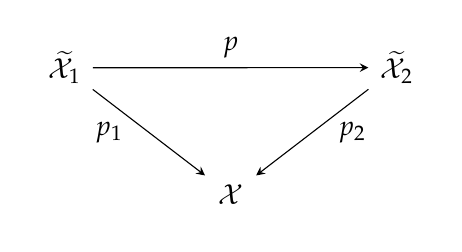
\begin{tikzpicture}
\matrix (m) [matrix of math nodes,row sep=3em,column sep=4em,minimum width=2em]
{
	\widetilde{\mathcal X}_1 & &\widetilde{\mathcal X}_2\\ 
	& {\mathcal X}\\};
\path[-stealth]
(m-1-1) edge node [above] {$p$} (m-1-3)
(m-1-1) edge node [left]  {$p_1~~$} (m-2-2)
(m-1-3) edge node [right] {$~~p_2$} (m-2-2);
\end{tikzpicture}
\\
where $\sX$ is locally connected and $p_1$, $p_2$ are covering projections. If $p$ is a surjection then $p$ is a covering projection.
\end{corollary}
\begin{theorem}\label{top_locally_conn_cov_com_thm}\cite{spanier:at}
	If   $p: \widetilde{\mathcal X}\to {\mathcal X}$ is a covering projection onto locally connected base space, then for any component  $\widetilde{\mathcal Y}$ of $\widetilde{\mathcal X}$ the map
	$$
	p|_{\widetilde{\mathcal Y}}:\widetilde{\mathcal Y} \to p\left(\widetilde{\mathcal Y} \right) 
	$$
	is a covering projection onto some component of $\widetilde{\mathcal X}$.
\end{theorem}
%\begin{lemma}\label{top_cov_cat_lem}
%In the {category of connected covering spaces} of a connected locally path-connected space every morphism is itself a covering projection.
%\end{lemma}
\begin{theorem}\label{top_conjugate_thm}\cite{spanier:at}
Let $p_1: 	\widetilde{\sX}_1 \to \sX$, $p_2: 	\widetilde{\sX}_2 \to \sX$ be objects  in the category of connected covering spaces of a connected locally path-connected space $\sX$. The following are equivalent
\begin{enumerate}
	\item [(a)] There is a coveting projection $f:\widetilde{\sX}_1 \to \widetilde{\sX}_2$ such that $p_2 \circ f = p_1$.
	\item[(b)] For all $\widetilde{x}_1\in \widetilde{\sX}_1$ and  $\widetilde{x}_2\in \widetilde{\sX}_2$ such that $p_1\left(\widetilde{x}_1 \right) = p_2\left(\widetilde{x}_2 \right)$, $\pi_1\left(p_1\right)\left( \pi_1 \left( \widetilde{\sX}_1, \widetilde{x}_1\right)  \right)$ is conjugate to a subgroup of  $\pi_1\left(p_2\right)\left( \pi_1 \left( \widetilde{\sX}_2, \widetilde{x}_2\right)  \right)$.
	\item[(c)] There exist $\widetilde{x}_1\in \widetilde{\sX}_1$ and  $\widetilde{x}_2\in \widetilde{\sX}_2$ such that $\pi_1\left(p_1\right)\left( \pi_1 \left( \widetilde{\sX}_1, \widetilde{x}_1\right)  \right)$ is conjugate to a subgroup of  $\pi_1\left(p_2\right)\left( \pi_1 \left( \widetilde{\sX}_2, \widetilde{x}_2\right)  \right)$.
\end{enumerate} 
\end{theorem}
\begin{lemma}\label{top_om_lem}\cite{spanier:at}
A local homeomorphism is an open map.
\end{lemma}
\subsection{Unique path lifting}
  \begin{empt}
	There is a significant problem in the algebraic topology, called the lifting problem. Let $p: \mathcal{E} \to \mathcal{B}$ and $f: \mathcal{X} \to \mathcal{B}$ continuous maps of topological spaces. The {\it lifting problem} \cite{spanier:at} for $f$ is to determine whether there is a continuous map $f': \mathcal{X} \to \mathcal{E}$ such that $f=p\circ f'$-that is, whether the dotted arrow in the diagram
	\newline
	\hspace*{\fill}
	\begin{tikzpicture}
	\matrix (m) [matrix of math nodes,row sep=3em,column sep=4em,minimum width=2em] {
		& \mathcal{E} \\
		\mathcal{X} & \mathcal{B} \\};
	\path[-stealth]
	(m-2-1.east|-m-2-2) edge node [below] {$f$}(m-2-2)
	(m-1-2) edge node [right] {$p$} (m-2-2)
	(m-2-1)      edge [dashed]  node[above] {$f'$} (m-1-2);
	\end{tikzpicture}
	\hspace{\fill}
	\newline
	corresponds to a continuous map making the diagram commutative. If there is such map $f'$, then $f$ can be {\it lifted} to $\mathcal{E}$, and we call $f'$ a {\it lifting} or {\it lift} of $f$.
	If $p$ is a covering projection and $\mathcal{X} = [0,1] \subset \mathbb{R}$ then $f$ can be lifted.
\end{empt}
\begin{defn}\label{top_path_lifting_defn}\cite{spanier:at}
	A continous map $p:\mathcal{E} \to \mathcal{B}$ is said to have the {\it unique path lifting} if, given paths $\omega$ and $\omega'$ in $E$ such that $p \circ \omega = p \circ \omega'$ and $\omega(0)=\omega'(0)$, then $\omega=\omega'$.
\end{defn}
\begin{thm}\cite{spanier:at}\label{spanier_thm_un}
	Let $p: \widetilde{\mathcal{X}} \to \mathcal{X}$ be a covering projection and let $f, g: \mathcal{Y} \to \widetilde{\mathcal{X}}$ be liftings of the same map (that is, $p \circ f = p \circ g$). If $\mathcal{Y}$ is connected and $f$ agrees with g for some point of $\mathcal{Y}$ then $f=g$.
\end{thm}
\begin{rem}
	From theorem \ref{spanier_thm_un} it follows that a covering projection has unique path lifting.
\end{rem}

 	\subsection{Regular and universal coverings}
 		\begin{defn}\label{top_regular_defn}\cite{spanier:at}
 		A fibration $p: \mathcal{\widetilde{X}} \to \mathcal{X}$ with unique path lifting is said to be  {\it regular} if, given any closed path $\omega$ in $\mathcal{X}$, either every lifting of $\omega$ is closed or none is closed.
 	\end{defn}
 	\begin{thm}\label{locally_path_thm}\cite{spanier:at}
 		Let $p: \widetilde{\mathcal X} \to \mathcal X$ be a fibration with unique path lifting and assume that a nonempty $\widetilde{\mathcal X}$ is a locally path-connected space. Then $p$ is regular if and only if for some $\widetilde{x}_0 \in  \widetilde{\mathcal X}$, $\pi_1\left(p\right)\pi_1\left(\widetilde{\mathcal X}, \widetilde{x}_0\right)$ is a normal subgroup of $\pi_1\left(\mathcal X, p\left(\widetilde{x}_0\right)\right)$.
 	\end{thm}
 	\begin{theorem}\label{top_cov_fact_thm}\cite{spanier:at}
 		Let $G$ be a properly discontinuous group of homeomorphisms of space $\mathcal Y$. Then the projection of $\mathcal Y$ to the orbit space $\mathcal Y/G$ is a covering projection. If $\mathcal Y$ is connected, this covering is regular and $G$ is its group of covering transformations, i.e. $G = G\left(\mathcal Y~|~\mathcal Y/G \right)$. 
 	\end{theorem}
 	\begin{lem}\label{top_cov_from_pi1_cor}\cite{spanier:at}
 		Let $p: \widetilde{\mathcal X} \to \mathcal X$ be a fibration with a unique path lifting. If $ \widetilde{\mathcal X}$ is connected and locally path-connected and $\widetilde{x}_0 \in \widetilde{\mathcal X}$ then $p$ is regular if and only if $G\left(\widetilde{\mathcal X}~|~{\mathcal X} \right)$ transitively acts on each fiber of $p$, in which case 
 		$$
 		\psi: G\left(\widetilde{\mathcal X}~|~{\mathcal X} \right) \approx \pi_1\left(\mathcal X, p\left( \widetilde{x}_0\right)  \right) / \pi_1\left( p\right)\pi_1\left(\widetilde{\mathcal X}, \widetilde{x}_0 \right).  
 		$$
 	\end{lem}
 \begin{remark}\label{top_sim_con_reg_rem}\cite{spanier:at}
 If $\widetilde{   \sX}$ is simply connected, any fibration $p: \widetilde{   \sX} \to \sX$ is regular, and we also have the next result.
 \end{remark}
 	\begin{cor}\label{top_cov_pi1_cor}\cite{spanier:at}
 		Let $p: \widetilde{\mathcal X} \to \mathcal X$ be a fibration with a unique path lifting where $ \widetilde{\mathcal X}$ is simply connected locally path-connected and nonempty.  Then the group of self-equivalences of $p$ is isomorphic to the fundamental group of ${\mathcal X}$, i.e. $\pi_1\left( {\mathcal X}\right)\approx G\left(\left.\widetilde{\sX}~\right|\sX\right)$.  
 	\end{cor}
 \begin{definition}\label{top_uni_cov_defn}\cite{spanier:at}
 	A \textit{universal covering space} of a connected space $\sX$ is an object $p: \widetilde{\sX}\to \sX$ of the category of connected covering spaces of $\sX$ such that for any object $p': \widetilde{\sX}'\to \sX$ of this category there is a morphism 
 	\newline
 	\begin{tikzpicture}
 	\matrix (m) [matrix of math nodes,row sep=3em,column sep=4em,minimum width=2em]
 	{
 		\widetilde{\sX}  &  & \widetilde{\sX}'\\
 		& \sX & \\};
 	\path[-stealth]
 	(m-1-1) edge node [above] {$f$} (m-1-3)
 	(m-1-1) edge node [left]  {$p~~$} (m-2-2)
 	(m-1-3) edge node [right] {$~~p'$} (m-2-2);
 	%\draw[dashed,->]   (m-1-1) -- (m-1-3);
 	\end{tikzpicture}
 	\\
 	in the category.
 \end{definition}
 
 \begin{lem}\label{top_simply_con_cov_lem}\cite{spanier:at}
 	A connected locally path-connected space $\mathcal X$ has a simply connected covering space if and only if  $\mathcal X$ is semilocally 1-connected.
 \end{lem}
 %\begin{lem}\label{top_simply_con_uni_cor}\cite{spanier:at}
 %	Any universal covering space of a connected locally path connected semilocally 1-connected space is simply connected.
% \end{lem}
 %\begin{lem}\label{top_uni_spa_lem}\cite{spanier:at}
% 	Two universal covering spaces of a connected locally path-connected space are equivalent.
% \end{lem}
 
  \begin{lem}\label{top_uni_exist_spa_lem}\cite{spanier:at}
 A simply connected covering space of a connected locally path-connected space $\sX$ is an universal covering space of $\sX$.
 \end{lem}
 
 
 	\section{Vector bundles}\label{top_vb_sub_sub}
 	\paragraph*{}
 	Let $k$ be the field of real or complex numbers, and let $\sX$ be a topological space.
 	\begin{definition}\cite{karoubi:k}
 		A \textit{quasi-vector bundle with base} $\mathcal X$ is given by:
 		\begin{enumerate}
 			\item [(a)] A finite dimensional $k$-vector space $E_x$ for every point $x$ of $\mathcal X$.
 			\item[(b)] A topology on the disjoint union $E = \bigsqcup E_x$ which induces the natural topology on each $E_x$, such that the obvious projection $\pi: E \to  \mathcal X$ is continuous.
 		\end{enumerate}
 		The quasi-vector bundle with base will be denoted by $\xi = \left( E, \pi, \mathcal X\right)$. The space $E$ is the \textit{total space} of $\xi$ and $E_x$ is the \textit{fiber} of $\xi$ at the point $x$.
 	\end{definition}
\begin{empt}\label{trivial_vb_empt}
	Let $V$ be a finite dimensional vector space over $k$,  $E_x = V$ and the total space may be identified with $\sX \times V$ with the product topology then the quasi-vector bundle  $\left(\sX \times V, \pi, \mathcal X\right)$ is called a \textit{trivial vector bundle}.
\end{empt}
\begin{empt}
Let $\xi = \left( E, \pi, \mathcal X\right)$ be a quasi-vector bundle, and let let $\sX' \subset \sX$ be a subspace of $\sX$. The triple $\xi' = \left(\pi^{-1}\left( \sX'\right) , \pi|_{\pi^{-1}\left( \sX'\right)}, \mathcal X'\right)$ is called the \textit{restriction} of $\xi$ to $\sX'$. The fibers of $\xi'$ are just fibers of $\xi$ over the subspace $\xi$. One has
\be
\sX'' \subset \sX' \subset \sX \quad \Rightarrow\quad \left.\left(\xi|_{\sX'} \right) \right|_{\sX''}= \xi|_{\sX''}.
\ee
\end{empt}
 \begin{definition}\label{top_vb_defn}
 	Let $\xi = \left( E, \pi, \mathcal X\right)$ be quasi-vector bundle. Then $\xi$ is said to be \textit{locally trivial} or a \textit{vector bundle} if for every point $x$ in $\sX$, there exists a neighborhood of $x$ such that $\xi|_{\sU}$ is isomorphic to a trivial bundle.
 \end{definition}
\begin{definition}\label{top_vb_cs_defn}
Let $\xi = \left( E, \pi, \mathcal X\right)$ be a {vector bundle}. Then a \textit{continuous section} of $\xi$ is a continuous map $s: \sX \to E$ such that $\pi \circ s = \Id_{\sX}$,
\end{definition}
 	\begin{remark}
 		In \cite{karoubi:k} the vector bundles over fields $\R$ and $\C$ are considered. Here we consider complex vector bundles only.
 	\end{remark}
% 	We refer to \cite{karoubi:k} for a notion of {\it (locally trivial) vector bundle}. 	Any {\it (locally trivial) vector bundle} with base $\mathcal X$ is a special case of \textit{quasi-vector bundle} which is a triple $\left(E, \pi, \mathcal X \right)$. 
 	\begin{definition}\label{vb_inv_img_funct_defn}\cite{karoubi:k}
 		Let $f: \mathcal X' \to \mathcal X$ be a continuous map. For every point $x'$ of $\mathcal X'$, let $E'_{x'}= E_{f\left(x' \right) }$. Then the set $E' = \bigsqcup_{x' \in \mathcal X'}$ may be identified with the \textit{fiber product} $\mathcal X' \times_{\mathcal X} E$ formed by the pairs $\left(x',e \right)$ such that $f\left(x' \right) = \pi\left( e\right)$. If  $\pi': E' \to \mathcal X'$ is defined by $\pi'\left(x',e \right) = x'$, it is clear that the triple $\xi = \left( E', \pi', \mathcal X'\right)$ defines a quasi-vector bundle over $ \mathcal X'$, when we provide $E'$ with the topology induced by $ \mathcal X' \times E$. We write $\xi' = f^*\left(\xi \right)$ or $f^*\left(E \right)$: this is the \textit{inverse image} of $\xi$ by $f$.  
 	\end{definition}
 
 	\begin{definition}\label{vb_cont_sec_defn}
 		If $\left( E, \pi, \mathcal X\right)$ is a quasi-vector bundle then a continuous map $s: \mathcal X\to E$ is said to be a \textit{continuous section} if $\pi \circ s = \Id_{ \mathcal X}$.  The space $\Ga\left({\mathcal X}, {E}\right)$, of continuous sections can be regarded as both left and right $C_b\left(\mathcal{X} \right)$-module.
 	\end{definition}
 
 \begin{theorem}\label{serre_swan_thm}\cite{karoubi:k}.
 	Theorem (Serre, Swan). Let $A = C_k(\sX)$ be the ring of continuous 
 	functions on a compact space $\sX$ with values in $k$. Then the section functor $\Ga$ induces an 
 	equivalence of categories of vector bundles over $\sX$ and finitely generated projecive $A$-modules.
 \end{theorem}
 	
 	%\begin{definition}\label{vb_inv_img_funct_defn}
 	%	If $f: \mathcal X \to \mathcal Y$ is a continuous map then there is an {\it inverse image functor}  $f^*:\mathrm{Vect}(\mathcal{Y})\to\mathrm{Vect}(\mathcal{X})$ (cf. \cite{karoubi:k}). 
 	%\end{definition}
 	
 	
 	
 	%Following fact is an implication of definitions.
 	%\begin{fact}\label{inv_image_fact}
 	%	A map $\varphi^*$ is an inverse image of $\varphi$ if and only if the above diagram is commutative for any $\mathcal U$ such that $\pi |_{\mathcal U}: \mathcal U \to \pi ({\mathcal U})$ is a homeomorphism.
 	%\end{fact}
 	
 	\begin{empt}\label{top_herm_bundle_empt}
 		Let $\mathcal X$ be a compact topological space and $\SS$ the complex vector bundle on $\mathcal X$, such for any  $x \in \mathcal{X}$ the fiber $\SS_x$ of $\SS$ is a Hilbert space, i.e. there is a scalar product.
 		\be\label{top_bundle_scalar_eqn}
 		\left( \cdot, \cdot \right)_x: \SS_x \times \SS_x \to \C.
 		\ee
 		 If $\Ga\left( M, S\right) $ is the space of continuous sections
 		of $S$ then we suppose that for any $\xi, \eta \in  \Ga\left( M, S\right)$ the map $\mathcal X \to \C$ given by $x \mapsto \left( \xi_x, \eta_x\right)_x$ is continuous. If    $\mu_{\mathcal{X}}$ is a measure on $\mathcal X$ then there is the scalar product $\left( \cdot, \cdot \right) :  \Ga\left( M, \SS\right) \times \Ga\left( M, \SS\right) \to \C$ given by
 	\be\label{top_bundle_herm_scalar_eqn}
 		\left( \xi, \eta\right)\stackrel{\text{def}}{=} \int_{\mathcal X}\left( \xi_x, \eta_x\right)_xd~\mu_{\mathcal{X}}
 	\ee
 		Denote by $L^2\left( \mathcal X, \SS, \mu_{\mathcal X}\right) $ or $L^2\left( \mathcal X, \SS\right) $ the Hilbert norm completion of $\Ga\left( M, S\right) $, and denote by $\left( \cdot, \cdot \right)_{L^2\left( \mathcal X, \SS, \mu_{\mathcal X}\right)}$ or $\left( \cdot, \cdot \right)_{L^2\left( \mathcal X, \SS\right)}$ the given by \eqref{top_bundle_herm_scalar_eqn} scalar product.
 		There is the natural representation
 		\begin{equation}\label{comm_bundle_repr_eqn}
 		C_0\left(\mathcal{X} \right) \to B\left( L^2\left( \mathcal X, \SS\right)\right). 
 		\end{equation}
 	\end{empt}
 	\begin{defn}\label{top_herm_bundle_defn}
 		In the situation of \ref{top_herm_bundle_empt} we say that $S$ is \textit{Hermitian vector bundle}.
 	\end{defn}
 
 
 \chapter{Algebra}
 \section{Algebraic Morita equivalence}
 
 \begin{defn}\label{morita_ctx_defn}
 	A \textit{Morita context} $\left( A,B,P,Q,\varphi,\psi\right)$ or, in some authors (e.g. Bass \cite{bass}) the \textit{pre-equivalence data} is a generalization of Morita equivalence between categories of modules. In the case of right modules, for two associative $\mathbf{k}$-algebras (or, in the case of $\mathbf{k} = \mathbb{Z}$, rings) $A$ and $B$, it consists of bimodules $_AP_B$, $_BQ_A$ and bimodule homomorphisms $\varphi: P\otimes_B Q\to A$, $\psi: Q\otimes_A P\to B$ satisfying mixed associativity conditions, i.e. for any $p,p' \in P$ and $q,q' \in Q$ following conditions hold:
 	\begin{equation}\label{morita_ctx_eqn}
 	\begin{split}
 	\varphi\left(p\otimes q \right) p' = p \psi\left(q\otimes p' \right),\\
 	\psi\left(q \otimes p \right) q' = q\varphi\left(p\otimes q' \right).  
 	\end{split}
 	\end{equation}
 	A Morita context is a \textit{Morita equivalence} if both $\varphi$ and $\psi$ are isomorphisms of bimodules. 
 \end{defn}
 
 \begin{rem}\label{morita_rem}
 	The Morita context $\left( A,B,P,Q,\varphi,\psi\right)$  is a Morita equivalence if and only if $A$-module $P$ is a finitely generated projective generator (cf. \cite{bass} II 4.4)
 \end{rem}
 
% \begin{cordefn}\label{invert_mod_defn}\cite{bass}
% 	Let $R$ be a commutative ring, and let $A$, $B$ be $R$-algebras
% 	We call a left $A\otimes_RB^\circ$ module $M$ \textit{invertible} if it satisfies to the following conditions, which are equivalent:
% 	\begin{enumerate}
% 		\item [(a)] $\otimes_{A}M:~ mod$-$A \xrightarrow{\approx} mod$-$B$ is an equivalence.
% 		\item[(b)] There is a left left $B\otimes_RA^\circ$ module $N$ such that $M\otimes_BN \cong A$ and $N\otimes_AM \cong B$ as bimodules.
% 		\item [(c)] $M\otimes_{B}:~B$-$mod \xrightarrow{\approx} ~B$-$mod$ is an equivalence.
% 	\end{enumerate}
 %\end{cordefn}
% \begin{empt}\label{invert_mod_auto_empt}\cite{bass}
% 	For any $R$-algebra $A$ write $\mathbf{Pic}_R\left(A \right)$  for the category of invertible $A\otimes_RA^\circ$ modules and bimodule isomorphisms. For any $\al, \bt \in \Aut_{R\mathrm{-alg}}\left(A \right)$ denote by $_\al A_\bt$ the $A\otimes_RA^\circ$ module such that there is $R$-linear isomorphism $\varphi: A \xrightarrow{\approx}_\al A_\bt$ and following condition holds
% 	\be\label{pic_act_eqn}
% 	a\varphi\left(x \right)b = \varphi\left(\al\left(a \right) x\bt\left(b\right)  \right); \quad \forall a, x, b \in A. 
% 	\ee	
% \end{empt}
 
% \begin{proposition}\label{invert_mod_auto_prop}
% 	Let $A$ be an $R$-algebra and let  $\al, \bt, \ga \in \Aut_{R\mathrm{-alg}}\left(A \right)$.
 %	\begin{enumerate}
 %		\item [(i)] $_\al A_\bt \cong _{\ga\al} A_{\ga\bt}$ as bimodules.
% 		\item[(ii)] $_{\Id_A} A_{\al}\otimes_A ~_{\Id_A} A_{\al} \cong _{\Id_A} A_{\al\bt}$ as bimodules.
% 		\item[(iii)] 
% 		$$
% 		_{\Id_A} A_{\al} \cong _{\Id_A}A_{\Id_A} \Leftrightarrow \al \mathrm{~is~an~inner~automorphism}.
% 		$$
 %		\item[(iv)] If $P \in \mathbf{Pic}_R\left(A \right)$ and if $P\cong A$ as left $A$-modules then $P\cong _{\Id_A} A_{\al}$ as bimodules for some $\al \in  \Aut_{R\mathrm{-alg}}\left(A \right)$.
% 	\end{enumerate}
% \end{proposition}

		\section{Finite Galois coverings}\label{fin_gal_cov_sec}
\paragraph*{} Here I follow to \cite{auslander:galois}. Let $A \hookto \widetilde{A}$ be an injective homomorphism of unital algebras, such that
\begin{itemize}
	\item $\widetilde{A}$ is a projective finitely generated $A$-module,
	\item There is an action $G \times \widetilde{A} \to \widetilde{A}$ of a finite group $G$ such that $$A = \widetilde{A}^G=\left\{\widetilde{a}\in \widetilde{A}~|~g\widetilde{a}=\widetilde{a}; ~\forall g \in G\right\}.$$
\end{itemize}
Let us consider the category $\mathscr{M}^G_{\widetilde{A}}$ of $G-\widetilde{A}$ modules, i.e.  any object $M \in \mathscr{M}^G_{\widetilde{A}}$ is a $\widetilde{A}$-module with equivariant action of $G$, i.e. for any $m \in M$ a following condition holds
$$
g\left(\widetilde{a}m \right)=  \left(g\widetilde{a} \right) \left(gm \right) \text{ for any } \widetilde{a} \in \widetilde{A}, ~ g \in G.
$$
Any morphism $\varphi: M \to N$ in the category $\mathscr{M}^G_{\widetilde{A}}$ is $G$- equivariant, i.e.
$$
\varphi\left( g m\right)= g \varphi\left( m\right)   \text{ for any } m \in M, ~ g \in G.
$$
Let $\widetilde{A}\left[ G\right]$ be an algebra such that $\widetilde{A}\left[ G\right] \approx \widetilde{A}\times G$ as an Abelian group and a multiplication law is given by
$$
\left( a, g\right)\left( b, h\right) =\left(a\left(gb \right), gh  \right).
$$
The category $\mathscr{M}^G_{\widetilde{A}}$ is equivalent to the category $\mathscr{M}_{\widetilde{A}\left[ G\right]}$ of $\widetilde{A}\left[ G\right]$ modules. Otherwise in \cite{auslander:galois} it is proven that if $\widetilde{A}$ is a finitely generated, projective $A$-module then there is an  equivalence between a category $\mathscr{M}_{A}$ of $A$-modules and the category $\mathscr{M}_{\widetilde{A}\left[ G\right]}$. It turns out that the category $\mathscr{M}^G_{\widetilde{A}}$ is equivalent to the category $\mathscr{M}_{A}$. The equivalence is given by mutually inversed functors $\left( -\right) \otimes \widetilde{A}: \mathscr{M}_{A} \to \mathscr{M}^G_{\widetilde{A}}$ and $\left( -\right) ^G: \mathscr{M}^G_{\widetilde{A}}\to \mathscr{M}_{A}$.






\section{Profinite and residually finite groups}\label{profinite_section}
\begin{empt}\label{prof_empt}\cite{dix:profinite}
	Let $G$ be a group and $\left\{G_\al \right\}$ be the set of all normal subgroups of finite index in $G$. Then the set $\left\{G/G_\al, \phi_{\al\bt}\right\}$ of finite quotients $G/G_\al$, of $G$ together with the canonical projections $\phi_{\al\bt}:G/G_\al \to G/G_\bt$  whenever $G_\al \subset G_\bt$ is an inverse system. The inverse limit $\varprojlim G/G_\a$ of this system is called the \textit{profinite completion} of $G$ and is denoted by $\widehat{G}$. The group $\widehat{G}$ can also be described as the closure of the image of $G$ under the
	the diagonal mapping $\Delta : G \to \prod \left( G/G_\a\right)$  where $G/G_\a$, is given the discrete topology and $\prod \left( G/G_\a\right)$ has the product topology. In this description the elements of $\widehat{G}$ are the
	elements $\left(g_\a \right) \in \prod \left( G/G_\a\right)$ which satisfy $\phi_{\al\bt}\left( g_\al\right)= \bt$  whenever $G_\a \subset G_\bt$.
\end{empt} 
%\begin{theorem}\label{profinite_thm}\cite{dix:profinite}
%	Let $G$ and $H$ be finitely generated groups, and let $\widehat{G}$ (resp. $\widehat{H}$) be the profinite completion of $G$ (resp. $H$), Then $\widehat{G}$ and $\widehat{H}$ are isomorphic as topological groups id the set of isomorphism classes of finite quotients  of $G$ is equal the set of isomorphism classes of finite quotients  of $H$.
%\end{theorem}

\begin{definition}\label{residually_finite_defn}\cite{bogopolsky:group_theory}
	A group $G$ is said to be \textit{residually finite} if for each nontrivial element from $G$ there exists a finite group $K$ and a homomorphism $\varphi: G\to K$ such that $\varphi\left( g\right) \neq 1$.
\end{definition}

%\section{Miscellany}

% \begin{theorem}\label{noeter_skolem_thm}\cite{pierce:ass}
% Let $F$ be a field, and let $A$ be a finite-dimensional simple central $F$-algebra. Suppose that $B$ is a simple subalgebra of $A$. If $\chi$ is an algebra homomorphism of $B$ to $A$ then there exists an invertible element $u \in A$ such that $\chi\left(y \right) = u^{-1}yu$ for all $y \in B$.
% \end{theorem}
 
 
 %\begin{theorem}[Morita \cite{Morita:58}, \cite{Morita:65}]
 %	\label{the:ProGenMorita}
 %	Let~$R$ be a ring with unit and~$Q$ a right $R$-module.  Then~$Q$ induces a
 %	Morita equivalence between~$R$ and $R'\subset\End(Q)$ if and only if~$Q_R$ is
 %	a finitely generated projective generator.%\footnote{An object~$X$ in an 		Abelian category is a generator iff every object is a quotient of a direct 		sum of copies of~$X$.}
 %\end{theorem}

 \begin{definition}\label{normal_subgroup_defn}\cite{kurosh:lga}
 A subgroup $H$ is called a \textit{normal subgroup} (or \textit{invariant subgroup}) of the group $G$, if the left-sided partition of the group $G$
 with respect to the subgroup $H$ coincides with the right-sided
 partition, i.e. if for every $g\in G$ the equation
 \be\label{normal_subgroup_eqn}
 gH = Hg
 \ee
 holds (understood in the sense that the two subsets coincide in $G$).
 Thus we can speak simply of \textit{the partition of the group} $G$ \textit{with
 respect to the normal subgroup} $H$.
 \end{definition}
 
 \chapter{Functional analysis}

\section{Weak topologies}

\begin{definition}\label{w_topology_defn}\cite{rudin:fa}
 Suppose $X$ is a topological vector space (with topology $\tau$) whose dual $X^*$ separates points on $X$.   The $X^*$-topology (cf. Definition \ref{f_topology_defn}) of $X$ is called the 
weak topology of $X$.
\end{definition}

\begin{definition}\label{w*_topology_defn}\cite{rudin:fa}
	% The \textit{weak}$*$-topology of a dual space 
	 Let $X$ again be a  	topological vector space whose dual is $X^*$. For the definitions that follow, it is irrelevant whether $X^*$ separates points on X or not. The important  observation to make is that every $x\in X$ induces a linear functional $f_x$ on $X^*$, 
	defined by 
	$$
	f_x\La= \La x
	$$
%	and that $\left\{\left.f_x\right|x \in X\right\}$ separates points on $X^*$. 	The linearity of each $f_x$ is obvious; if/^A =/xA' for all x e X, then 
%	Ax = A'x for all x, and so A = A' by the very definition of what it means 
%	for two functions to be equal. 
%	We are now in the situation described by Theorem 3.10, with X* in 
%	place of X and with X in place of X'. 
	The $X$-topology of $X^*$ (cf. Definition \ref{f_topology_defn}) is called the \textit{weak}*-\textit{topology of} $X^*$.
	
\end{definition}
\begin{remark}\label{weak_convergence_rem}\cite{rudin:fa}
In the above situation the net $\left\{x_\a\right\}_{\a\in \mathscr A}\in X$ is convergent with respect to weak topology if the net $\left\{\La x_\a\right\}\in \C$ is convergent for all $\La \in X^*$. Similarly the net $\left\{\La_\a\right\}_{\a\in \mathscr A}\in X^*$ is convergent with respect to weak*-topology if the net $\left\{\La_\a x\right\}\in \C$ is convergent for all $x\in X$.
\end{remark}


 \section{Fourier transformation}
 \paragraph*{}
 There is a norm on $\mathbb{Z}^n$ given by
 \begin{equation}\label{mp_znorm_eqn}
 \left\|\left(k_1, ..., k_n\right)\right\|= \sqrt{k_1^2 + ... + k^2_n}.
 \end{equation}
 The space of complex-valued Schwartz  functions on $\Z^n$ is given by 
 \begin{equation}\label{schwartz_z_eqn}
 \sS\left(\mathbb{Z}^n\right)\bydef \left\{a = \left\{a_k\right\}_{k \in \mathbb{Z}^n} \in \mathbb{C}^{\mathbb{Z}^n}~|~ \mathrm{sup}_{k \in \mathbb{Z}^n}\left(1 + \|k\|\right)^s \left|a_k\right| < \infty, ~ \forall s \in \mathbb{N} \right\}.
 \end{equation}
 
 
 Let $\mathbb{T}^n$ be an ordinary $n$-torus. We will often use real coordinates for $\mathbb{T}^n$, that is, view $\mathbb{T}^n$ as $\mathbb{R}^n / \mathbb{Z}^n$. Let $\Coo\left(\mathbb{T}^n\right)$ be an algebra of infinitely differentiable complex-valued functions on $\mathbb{T}^n$. 
 There is the bijective Fourier transformations  $\mathcal{F}_\T:\Coo\left(\mathbb{T}^n\right)\xrightarrow{\approx}\sS\left(\mathbb{Z}^n\right)$;  $f \mapsto \widehat{f}$ given by
 \begin{equation}\label{nt_fourier_eqn}
 \widehat{f}\left(p\right)= \mathcal F_\T (f) (p)= \int_{\mathbb{T}^n}e^{- 2\pi i x \cdot p}f\left(x\right)dx
 \end{equation}
 where $dx$ is induced by the Lebesgue measure on $\mathbb{R}^n$ and   $\cdot$ is the  scalar
 product on the Euclidean space $\R^n$.
 The Fourier transformation carries multiplication to convolution, i.e.
 \begin{equation*}
 \widehat{fg}\left(p\right) = \sum_{r +s = p}\widehat{f}\left(r\right)\widehat{g}\left(s\right).
 \end{equation*}
 The inverse Fourier transformation $\mathcal{F}^{-1}_\T:\sS\left(\mathbb{Z}^n\right)\xrightarrow{\approx} \Coo\left(\mathbb{T}^n\right)$;  $ \widehat{f}\mapsto f$ is given by
 $$
 f\left(x \right) =\mathcal{F}^{-1}_\T \widehat f\left( x\right)  = \sum_{p \in \Z^n} \widehat f\left( p\right)   e^{ 2\pi i x \cdot p}.
 $$
 There  is the $\C$-valued scalar product  on $\Coo\left( \T^n\right)$ given by
 $$
 \left(f, g \right) = \int_{\T^n}fg dx =\sum_{p \in \Z^n}\widehat{f}\left( -p\right) \widehat{g}\left(p \right).  
 $$ 
 Denote by $\SS\left( \R^{n}\right) $ be the space of
 complex Schwartz (smooth, rapidly decreasing) functions on $\R^{n}$. 
 \be\label{mp_sr_eqn}
 \begin{split}
 	\SS\left(\mathbb {R} ^{n}\right)=\\
 	=\left\{f\in C^{\infty }(\mathbb {R} ^{n}):\|f\|_{\alpha  ,\beta )}<\infty \quad \forall \alpha 
 	=\left( \al_1,...,\al_n\right) ,\beta =\left( \bt_1,...,\bt_n\right)\in \mathbb {Z} _{+}^{n}\right\},\\
 	\|f\|_{{\alpha ,\beta }}=\sup_{{x\in {\mathbb  {R}}^{n}}}\left|x^{\alpha }D^{\beta }f(x)\right|
 \end{split}
 \ee
 where 
 \bean
 x^\al = x_1^{\al_1}\cdot...\cdot x_n^{\al_n},\\
 D^{\beta} = \frac{\partial}{\partial x_1^{\bt_1}}~...~\frac{\partial}{\partial x_n^{\bt_n}}.
 \eean
 The topology on $\SS\left(\mathbb {R} ^{n}\right)$ is given by seminorms $\|\cdot\|_{{\alpha ,\beta }}$.
 %\begin{defn}\label{nt_*w_defn}
% 	Denote by $\SS'\left( \R^{n}\right) $ the vector space dual to $\SS\left( \R^{n}\right) $, i.e. the space of continuous functionals on $\SS\left( \R^{n}\right)$. Denote by $\left\langle\cdot, \cdot \right\rangle:\SS'\left( \R^{n}\right)\times	\SS\left( \R^{n}\right)\to\C$ the natural pairing. We say that $\left\{a_n \in \SS'\left(\mathbb {R} ^{n}\right)\right\}_{n \in \N}$ is \textit{weakly-* convergent} to $a \in \SS'\left(\mathbb {R} ^{n}\right)$ if for any $b \in  \SS\left(\mathbb {R} ^{n}\right)$ following condition holds
% 	$$
% 	\lim_{n \to \infty}\left\langle a_n, b \right\rangle = \left\langle a, b \right\rangle.	
% 	$$
% 	We say that
% 	$$
% 	a = \lim_{n\to \infty}a_n
% 	$$
% 	in the \textit{sense of weak-* convergence}.
% \end{defn}
 
 Let $\mathcal F$ and $\mathcal F^{-1}$ be the ordinary and inverse Fourier transformations given by
 \begin{equation}\label{intro_fourier}
 \begin{split}
 \left(\mathcal{F}f\right)(u) = \int_{\mathbb{R}^{2N}} f(t)e^{-2\pi it\cdot u}dt,~\left(\mathcal F^{-1}f\right)(u)=\int_{\mathbb{R}^{2N}} f(t)e^{2\pi it\cdot u}dt %,
 % \left(\widetilde{F}f\right)(u) = \int f(t)e^{it\cdot Ju}dt.~
 \end{split}
 \end{equation}
 which satisfy  following conditions
 $$
 \mathcal{F}\circ\mathcal{F}^{-1}|_{\SS\left( \R^{n}\right)} = \mathcal{F}^{-1}\circ\mathcal{F}|_{\SS\left( \R^{n}\right)} = \Id_{\SS\left( \R^{n}\right)}.
 $$
 There is the $\C$-valued scalar product  on $\SS\left( \R^n\right)$ given by
 \begin{equation}\label{fourier_scalar_product_eqn}
 \left(f, g \right) = \int_{\R^n}fg dx =\int_{\R^n}\mathcal{F}f\mathcal{F}g dx. 
 \end{equation}
 
 which if $\mathcal{F}$-invariant, i.e.
 \be\label{mp_inv_eqn}
 \left(f, g \right)_{L^2\left( \R^n\right) } = \left(\mathcal{F}f, \mathcal{F}g \right)_{L^2\left( \R^n\right) }.
 \ee
 
 There is the action of $\Z^n$ on $\R^n$ such that
 $$
 g x = x + g; ~ x \in \R^n,~ g \in \Z^n
 $$
 and $\T^n \approx \R^n / \Z^n$. Any $f \in \Coo\left( \T^n\right)$ can be regarded as $\Z^n$- invariant and smooth function on $\R^n$. On the other hand if $f \in \SS\left( \R^n\right)$ then the series 
 $$
 h = \sum_{g \in \Z^n} g f 
 $$ 
 is point-wise convergent and $h$ is a smooth $\Z^n$ - invariant function. So we can assume that $h \in \Coo\left(\T^n \right)$. This construction provides a map
 \begin{equation}\label{mp_sooth_sum_eqn}
 \begin{split}
 \SS\left(\R^n\right) \to  \Coo\left(\T^n\right), \\
 f \mapsto h = \sum_{g \in \Z^n} g f.
 \end{split}
 \end{equation}
 If $\widehat f = \mathcal F f$,  $\widehat h = \mathcal F_{\T} h$ then for any $p \in \Z^n$ a following condition holds
 \begin{equation}\label{fourier_from_r_to_z_eqn}
 \widehat h\left(p\right) = \widehat f\left( p\right). 
 \end{equation}  
 
 
% \section{Distributions}
 
% \begin{theorem}
 %6.28 Theorem 
 %Suppose $\La \in \mathscr D'\left(\Om\right)$. There exist continuous functions $g_\a$ in $\Om$, one for each multi-index $\a$, such that 
% \begin{enumerate}
% 	\item[(a)] each compact $K \subset \Om$ intersects the supports of only finitely many $g_\a$, and
% 	\item[(b)] $\La = \sum_\a D^\a g_a$.
% \end{enumerate}
% 	If $\La$ has finite order, then the functions $g_\a$ can be chosen so that only 
% 	finitely many are different from $0$. 
 %\end{theorem}
 
 %\begin{theorem}\label{radon_repr_thm}\cite{bogachev_measure_v2} (Riesz representation theorem)
 %$Theorem. 7.10.4 $
 % Let $K$ be a compact space. Then, for every continuous linear functional $L$ on the Banach space $C\left(K \right)$ , there exists a unique
% Radon measure $\mu$ such that
% $$
% L\left(f \right) = \int_{K} f ~\d\mu \quad \forall f \in C\left(K \right). 
% $$
% \end{theorem}
 
 
 
 
% \section{Miscellany}
 
% \begin{theorem}\label{dini_thm}\cite{rudin:pa}
 %7.13 
% Theorem Suppose $K$ is compact, and 
% \begin{enumerate}
% 	\item[(a)]  $\left\{f_n\right\}_{n \in \N}$ is a sequence of continuous functions on $K$, 
% \item[(b)]  $\left\{f_n\right\}$ converges point-wise to a continuous function $f$ on $K$, 
% \item[(c)] $f_n(x)\ge f_{n+l}(x)$ for all $x\in K$, $n = 1, 2, 3,...$. 
% \end{enumerate}
% Then $f_n \to f$ uniformly on $K$. 
% \end{theorem}
 %\begin{theorem}\label{spectral_thm}\cite{murphy}
%2.5.6. Theorem. 
%Let $u$ be a normal operator on a Hilbert space $\H$, and let $\sigma\left(u \right)$ be the spectrum of $u$.
%Then there is the unique spectral measure $E$ relative to $\left( \sigma\left(u %\right), \H\right)$  such that
%$u = \int z dE$, where $z$ is the inclusion map of $\sigma\left(u \right)$ in $\C$.
%\end{theorem} 

\chapter{Operator algebras}



\section{$C^*$-algebras and von Neumann algebras}
\paragraph{}In this section I follow to \cite{murphy,pedersen:ca_aut}.
\begin{definition}\cite{murphy}
	A \textit{Banach *-algebra} is a *-algebra $A$ together with a complete submultiplicative norm such that $\left\| a^*\right\|=\left\| a\right\| ~\forall a\in A$. If, in addition, $A$ has a unit
	such that $\left\| 1\right\|=1$, we call $A$ a \textit{unital Banach *-algebra}.
	
	A \textit{$C^*$-algebra} is a Banach *-algebra such that
	\be
	\left\| a^*a\right\|=\left\| a\right\|^2\quad \forall a\in A.
	\ee
\end{definition}
\begin{example}\cite{murphy}
	%	2.1.3. Ezample. 
	If $\H$ is a Hilbert space, then the algebra of bounded operators $B\left(\H\right)$ is a $C^*$-algebra. %We 		shall see that every C*-algebra can be thought of as a C*-subalgebra of 		some B(H) 
\end{example}
\begin{definition}\label{essential_defn}\cite{rae:ctr_morita}
	% Definition 2.35. 
	A two sided ideal $I$ in a $C^*$-algebra $A$
	is essential if $I$ 
	has nonzero intersection 
	with every other nonzero ideal $A$. 
\end{definition}
Alternatively the essential ideal can be given by the following lemma.
\begin{lemma}\label{essential_lem}\cite{rae:ctr_morita}
	%Lemma 2.36. 
	An ideal $I$ 
	is essential if and only if $aI= \left\{0\right\}$
	implies $a 
	=0$.
\end{lemma}
\begin{example}\label{comm_ess_exm}\cite{rae:ctr_morita}
%Example 2.37. 
Let $A\bydef C_0\left( \sX\right)$ and let $\sU$ be an open subset of X. Then 
$$
I\bydef \left(\left.f\in A\right| f\left(x\right)= 0 \quad \forall x \in \sX\setminus\sU\right)
$$
	is an essential ideal in $A$ 
	if and only if $\sU$ 
	is dense 
	in $\sX$. 
\end{example}


\begin{defn}\label{unitization_defn}\cite{rae:ctr_morita}
	A \text{unitization} of a $C^*$-algebra $A$ is  a $C^*$-algebra $B$ with identity and an injective *-homomorphism $\iota: A \hookto B$ such that $\iota\left(A\right)$ is an essential ideal of $B$. 
\end{defn}

\begin{example}\label{unitization_exm}
	Suppose $A$ is  $C^*$-algebra which has no identity. Then $A^+ = A \oplus \C$
	is a *-algebra with 
	$$
	\left( a \oplus \la\right)\left( b \oplus \mu\right) = \left(ab + \la b + \mu a\right)  \oplus \la \mu, \quad \left(a \oplus \la \right)^* = a^*\oplus \overline{\la}. 
	$$
	It is proven in \cite{rae:ctr_morita} that there is the natural unique $C^*$-norm $\left\| \cdot\right\|_{A^+}$  on $A^+$ such that 
	$$
	\left\|a \oplus 0 \right\|_{A^+}=\left\|a \oplus 0 \right\|_{A}
	$$
	where $\left\|\cdot \right\|_{A}$ is the $C^*$-norm on $A$. Thus $A^+$ is an unital $C^*$-algebra, and the natural map $A\hookto A^+$ is a unitization.
\end{example}
\begin{definition}\label{multiplier_min_defn}
	Let $A$ be a $C^*$-algebra. The described in the Example \ref{unitization_exm} unitization   $\iota: A \hookto B$  is called \textit{minimal}.
\end{definition}
\begin{definition}\label{multiplier_max_defn}\cite{rae:ctr_morita}
	A unitization   $\iota: A \hookto B$  is called \textit{maximal} if for every embedding $j: A\hookto C$ of $A$ as an essential ideal of a $C^*$-algebra $\phi: C\to B$ such that $\phi \circ j = \iota$. 
\end{definition}

\begin{rem}\label{multiplier_rem}
	It is proven in \cite{rae:ctr_morita} that for any $C^*$-algebra $A$ there unique maximal unitization.
\end{rem}

\begin{definition}\label{multiplier_defn}
	We say that the maximal unitization of $A$ is the \textit{multiplier algebra} of $A$ and denote it by $M\left( A\right)$. 
\end{definition}
\begin{defn}\label{strict_topology}\cite{pedersen:ca_aut}
	Let $A$ be a $C^*$-algebra.  The {\it strict topology} on the multiplier algebra $M(A)$ is the topology generated by seminorms $\vertiii{x}_a = \|ax\| + \|xa\|$, ($a\in A$). If $\La$ is a directed set and $\left\{a_\la\in M\left( A\right) \right\}_{\la\in \La}$ is a net the we denote by $\bt\text{-}\lim_{\la\in\La }a_\la$ the limit of $\left\{a_\la \right\}$ with respect to the strict topology.
	If $x \in M(A)$  and a sequence of partial sums $\sum_{i=1}^{n}a_i$ ($n = 1,2, ...$), ($a_i \in A$) tends to $x$ in the strict topology then we shall write
	\begin{equation*}
	x = \bt\text{-}\lim\sum_{i=1}^{\infty}a_i.
	\end{equation*}
\end{defn}

\begin{defn}\label{app_unit_defn}\cite{pedersen:ca_aut}
	Let $A$ be a $C^*$-algebra. A net $\left\{u_\la \right\}_{\la \in \La}$ in $A_+$ with $\left\|u_\la \right\| \le 1$ for all $\la \in \La$ is called an \textit{approximate unit} for $A$ if $\la < \mu$ implies $u_\la < u_\mu$ and if $\lim \left\|x- xu_\la \right\| = 0$ for each $x$ in $A$. Then, of course, $\lim \left\|x- u_\la x \right\| = 0$ as well.
\end{defn}
\begin{thm}\label{app_unit_thm}\cite{pedersen:ca_aut}
	Each $C^*$-algebra contains an \textit{approximate unit}.
\end{thm}
\begin{proposition}\label{mult_str_pos_prop}\cite{apt_mult}
	If $B$ is a $C^*$-subalgebra of $A$ containing an
	approximate unit for $A$, then  $M\left(B \right) \subset M\left( A\right)$  (regarding $B''$ as a subalgebra	of $A''$).
\end{proposition}
\begin{definition}\label{hered_defn}\cite{pedersen:ca_aut}
	A cone $M$ in the positive part of $C^*$-algebra $A$ is said to be \textit{hereditary} if $0 \le x \le y$, $y \in M$ implies $x \in M$ for each $x \in A$. A *-subalgebra $B$ of $A$ is \textit{hereditary} if $B_+$ is hereditary in $A_+$.
\end{definition}
\begin{lemma}\label{hered_lem}\cite{murphy}
	Let $B$ be a $C^*$-subalgebra of $C^*$-algebra $A$. Then $B$ is hereditary in $A$ if and only if $bab' \in B$ for all $b, b' \in B$ and $a \in A$.
\end{lemma}
\begin{lemma}\label{hered_ideal_lem}\cite{murphy}
	Let $A$ be a $C^*$-algebra.
	\begin{enumerate}
		\item[(i)] If $L$ is a closed left ideal in $A$ then $L\cap L^*$ is a hereditary $C^*$-subalgebra of $A$. The map $L \mapsto L\cap L^*$ is the bijection from the set of closed left ideals of $A$ onto the the set of hereditary $C^*$-subalbebras of $A$.
		\item[(ii)] If $L_1, L_2$ are closed left ideals, then $L_1 \subseteq L_2$ is and only if $L_1\cap L_1^* \subset L_2\cap L_2^*$.
		\item[(iii)] If $B$ is a hereditary $C^*$-subalgebra of $A$, then the set 
		$$
		L\left(B \right) = \left\{\left.a \in A~\right| a^*a \in B \right\}
		$$
		is the unique closed left ideal of $A$ corresponding to $B$.
	\end{enumerate}
\end{lemma}

\begin{defn}\label{center_defn}\cite{murphy}
	If $A$ is a $C^*$-algebra, its \textit{center} $C$ is the set of elements of $A$ commuting with every of $A$.
\end{defn}
\begin{defn}
	\label{strong_topology_defn}\cite{pedersen:ca_aut} Let $\H$ be a Hilbert space. The {\it strong} topology on $B\left(\H\right)$ is the locally convex vector space topology associated with the family of seminorms of the form $x \mapsto \|x\xi\|$, $x \in B(\H)$, $\xi \in \H$.
\end{defn}
\begin{defn}\label{weak_topology_defn}\cite{pedersen:ca_aut} Let $\H$ be a Hilbert space. The {\it weak} topology on $B\left(\H\right)$ is the locally convex vector space topology associated with the family of seminorms of the form $x \mapsto \left|\left(x\xi, \eta\right)\right|$, $x \in B(\H)$, $\xi, \eta \in \H$.
\end{defn}

\begin{thm}\label{vN_thm}\cite{pedersen:ca_aut}
	Let $M$ be a $C^*$-subalgebra of $B(\H)$, containing the identity operator. The following conditions are equivalent:
	\begin{itemize}
		\item $M=M''$ where $M''$ is the bicommutant of $M$;
		\item $M$ is weakly closed;
		\item $M$ is strongly closed.
	\end{itemize}
\end{thm}


\begin{defn}\cite{pedersen:ca_aut}
	Any $C^*$-algebra $M$ is said to be a {\it von Neumann algebra} or a {\it $W^*$- algebra} if $M$ satisfies to the conditions of the Theorem \ref{vN_thm}.
\end{defn}
\begin{definition}\label{factor_defn}\cite{pedersen:ca_aut}
	We say that a  von Neumann algebra $M$ is 	a \textit{factor} if the center of consists only of scalar multiplies of $1_M$.
\end{definition}


%\begin{defn}\cite{pedersen:ca_aut}
%Let $B \in B(H)$ be a $C^*$-algebra. Denote by $B''$ the strong closure of $B$ in $B(H)$. $B''$ is an unital weakly closed $C^*$-algebra and if $B$ acts non-degenerately on $H$ then  $B''$ is the {\it bicommutant} of $B$. Any strongly (=weakly) closed algebra is said to be a {\it von Neumann algebra}.
%\end{defn}
%\begin{defn}\cite{pedersen:ca_aut}
%For any $x\in B(H)$ element $|x| \stackrel{\text{def}}{=} (xx^*)^{1/2}$ is said to be the {\it absolute value of} $x$.
%\end{defn}
\begin{lem}\label{increasing_convergent_w_lem}\cite{pedersen:ca_aut} Let $\Lambda$ be an increasing in the partial ordering.  Let $\left\{x_\lambda \right\}_{\la \in \La}$ be an increasing of self-adjoint operators in $B\left(\H\right)$, i.e. $\la \le \mu$ implies $x_\la \le x_\mu$. If $\left\|x_\la\right\| \le \ga$ for some $\ga \in \mathbb{R}$ and all $\la$ then $\left\{x_\lambda \right\}$ is strongly convergent to a self-adjoint element $x \in B\left(\H\right)$ with $\left\|x_\la\right\| \le \ga$.
\end{lem}
%\begin{defn}\label{range_proj_defn}\cite{pedersen:ca_aut}
%For each $x\in B(\H)$ we define the {\it range projection} of $x$ (denoted by $[x]$) as projection on closure of $x\H$. If $x\ge 0$ then the sequence $\left(\left((1 /n) +x\right)^{-1}x\right)$ is monotone increasing to $[x]$.  If $p$ and $q$ are projections then $p \vee q = [p + q]$ and thus $p \wedge q = 1 - \left[2 - \left(p+q\right)\right]$. Similarly we have $p \setminus q = p - p\wedge q$. Since $[x]\H$ is the orthogonal complement of the null space of $x^*$ we have $[x]=[xx^*]$. 
%\end{defn}
%\begin{cor}
%If $M$ is a $W^*$-algebra and $a \in M$ then the range projection $[a]$ of $a$ lies in $M$.
%\end{cor}
%If $\mathcal{M}$ is a von Neumann algebra in $B(\H)$ then $[x]\in \mathcal{M}$ for any $x\in \mathcal{M}$. We next prove a {\it polar decomposition}.
\paragraph*{}    For each $x\in B(\H)$ we define the {\it range projection} of $x$ (denoted by $[x]$) as projection on the closure of $x\H$. If $M$ is a von Neumann algebra and $x \in M$ then $[x]\in M$.

\begin{prop}\label{polar_decomposition_prop}\cite{pedersen:ca_aut}
	For each element $x$ in   a von Neumann algebra $M$ there is a unique partial isometry $u\in M$ and positive $\left|x\right| \in M_+$ with $uu^*=[|x|]$ and  $x=|x|u$.
\end{prop}
\begin{defn}\label{polar_decomposition_defn}
	The formula $x=|x|u$ in the Proposition \ref{polar_decomposition_prop} is said to be the \textit{polar decomposition}.
\end{defn}


\begin{definition}\label{stritly_pos_defn}\cite{pedersen:ca_aut}
	%2.10.4	
	We say that an element $h$ is a $C^*$-algebra is \textit{strictly positive} if $\phi\left( h\right)>0$ for any nonzero positive linear functional $\phi$ on $A$.
\end{definition}
\begin{thm}\label{stritly_pos_thm}\cite{pedersen:ca_aut}
	Let $A$ be a $C^*$-algebra. The following conditions are equivalent:
	\begin{enumerate}
		\item [(i)] There is a strictly positive element $h$ in $A_+$.
		\item[(ii)] There is an element $h$ in $A_+$ such that $\left[ h\right] = 1$ in $A''$.
		\item[(iii)] There is a countable approximate unit for $A$.
	\end{enumerate}
\end{thm}
\begin{proposition}\label{stritly_pos_prop}\cite{blackadar:ko}
	%Proposition 12.3.1. 
	Let $A$ be a $C^*$-algebra, and $h \in A_+$. Then $h$ is strictly
	positive if and only if $hA$ is dense in $A$.
\end{proposition}
\begin{definition}\label{simple_ca_defn}\cite{pedersen:ca_aut}
	A $C^*$-algebra $A$ is said to be \textit{simple} if $0$ and $A$ are its only closed ideals. In this book we consider only simple $C^*$-algebras of compact operators $\K\left(\H \right)$ where $\H = \C^n$ ($n \in \N$) or $\H = \ell^2\left( \N\right)$. 
\end{definition}
\begin{thm}\label{peder_id_thm}  \cite{pedersen:ca_aut} 
	% THEOREM 5.6.1
	For each $C^*$-algebra $A$ there is a dense hereditary ideal $K(A)$,
	which is minimal among dense ideals.
	
\end{thm}

\begin{defn}\label{peder_id_defn}
	The ideal $K(A)$ from the theorem \ref{peder_id_thm} is said to be the {\it Pedersen's ideal of $A$}. %Henceforth Pedersen's ideal shall be denoted by $K(A)$.
\end{defn}


%	If $\mathcal X$ is compact then we can select the a measure such that
%\begin{equation*}
%	\int_{\mathcal X}1_{\mathcal X} \ d\mu = 1.
%	\end{equation*}
%		\begin{equation*}
%		\int_{\mathcal X}\left|f\right| \ d\mu \le \left\|f\right\|_\infty;~~\forall f \in L^\infty\left(\mathcal X\right). 
%		\end{equation*}
%		If $\widetilde{\pi}: \widetilde{\mathcal X} \to \mathcal X$ is a covering then there is the measure $\widetilde{\mu}$ on $ \widetilde{\mathcal X}$ such that for any open relatively compact $\widetilde{\mathcal U} \subset \widetilde{\mathcal X}$ homeomorphically mapped onto $\widetilde{\pi}\left(\widetilde{\mathcal U}\right)$ following condition holds
%	\begin{equation*}
%	\widetilde{\mu}\left(\widetilde{\mathcal U}\right)= \mu\left(\widetilde{\pi}\left(\widetilde{\mathcal U}\right)\right)
%	\end{equation*}
%\paragraph{}For any self-adjoint operator $A \in B\left(H\right)$ and any bounded Borel-measured function $f$ on $\mathbb{R}$ there is the operator $f\left(A\right)\in B\left(H\right)$

%\begin{defn}
%In the above situation the $\widetilde{\mu}$ is said to be the $\widetilde{\pi}$-\textit{pullback} or simply \textit{pullback} of $\mu$. We will write $\mathfrak{pullback}_{\widetilde{\pi}}\left(\mu\right)\stackrel{\mathrm{def}}{=}\widetilde{\mu}$.
%\end{defn}
% \begin{defn}\cite{pedersen:ca_aut}
%  For any $x\in B(H)$ element $|x| \stackrel{\text{def}}{=} (xx^*)^{1/2}$ is said to be the {\it absolute value of} $x$.
%  \end{defn}
%  \begin{empt}\cite{pedersen:ca_aut}
% If $x\ge 0$ then the sequence $\left(\left((1 /n) +x\right)^{-1}x\right)$ is monotone increasing to $[x]$.  If $p$ and $q$ are projections then $p \vee q = [p + q]$ and thus $p \wedge q = 1 - \left[2 - \left(p+q\right)\right]$. Similarly we have $p \setminus q = p - p\wedge q$. Since $[x]H$ is the orthogonal complement of the null space of $x^*$ we have $[x]=[xx^*]$. If $\mathcal{M}$ is a von Neumann algebra in $B(H)$ then $[x]\in \mathcal{M}$ for any $x\in \mathcal{M}$. We next prove a {\it polar decomposition}.
%   \end{empt}

%  \begin{prop}\cite{pedersen:ca_aut}
%   For each element $x$ in   a von Neumann algebra $\mathcal{M}$ there is a unique partial isometry $u\in \mathcal{M}$ with $uu^*=[|x|]$ and  $x=|x|u$.
%   \end{prop}
%   \begin{proof}
%   Consider the sequence $u_n =x\left(\left(1/n\right)+ |x|\right)^{-1}$. Since $x=x[|x|]$ we have $u_n=u_n[x]$. A short computation shows that
%   \begin{equation}
%   (u_n - u_m)^*(u_n-u_m)=\left(\left(\left(1/n\right)+|x|\right)^{-1}-\left(\left(1/m\right)+|x|\right)^{-1}\right)|x|^2
%  \end{equation}
%  and this tends strongly, hence weakly to zero by spectral theory. It follows that $\{u_n\}$ is strongly convergent to an element $u\in \mathcal{M}$ with $u[|x|]=u$. Since $\{u_n|x|\}$ is norm convergent to $x$ we have $x=u|x|$. Then $x^*x= |x|u^*u|x|$ which implies that $u^*u \ge [|x|]$. Hence $u^*u = [|x|]$, in particular $u$ is a partial isometry. If $x = v|x|$ then from $v|x|=u|x|$ we get $v=v[|x|]=u$, so $u$ is unique.
%  \end{proof}




%\begin{defn}
%Let $a \in B(H)$, $h \in H$. The {\it $\sigma$-strong topology} is defined by the seminorms
%\begin{equation}
%p(a)= \sum_{i=1}^{\infty}ah_i, \ \sum_{i=1}^{\infty}\|h\|^2_i < \infty.
%\end{equation}
%\end{defn}

%\begin{defn}
%Let $X_B$ be a  Hilbert $B$-module, $B \to B(H)$ a faithful representation. For any $h \in H$  we define a seminorm $\vertiii{}_h$ on $_AX_B$ such that
% \begin{equation*}
% \vertiii{\xi}_h = \|\langle \xi, \xi \rangle_Bh\|.
% \end{equation*}
%  Completion of $X_B$ with respect to above seminorms is said to be the {\it strong completion}. Denote by $X''$ or $X''_{B''}$ the strong completion. There is the natural scalar product $\langle,\rangle_{X''}$ such that
% \begin{equation}
% \langle \xi, \zeta \rangle_{X''} \in B'',  \ \forall\xi,\zeta \in X''.
% \end{equation}
%  \end{defn}
% \begin{empt}
% Since $X\otimes_B H$ is norm complete there is a following natural $B$-isomorphism
%  \begin{equation}\label{von_neum_iso}
% X\otimes_B H \approx X''\otimes_{B''} H.
% \end{equation}
% \end{empt}
%\begin{thm}\label{mult_m_m_thm}\cite{pedersen:semi}
%	Let $A$ be a nonunital $C^*$-algebra, let  $A^m$ be a set of elements in $A''$ which can be approximated	weakly from below with self-adjoint operators of the form $x +\al$ a with $x \in A$ and $\al \in \R$. Denote by $A_m = - A^m$. The set $A^m \bigcap A_m$, is equal to the self-adjoint part of $M\left( A\right)$. 
%\end{thm}
\begin{theorem}\label{noncom_tietze_thm}\cite{apt_mult}
	Let $\pi$ be a surjective morphism between separable $C^*$-algebras $A$ and $B$. Then $\pi$ extends to a surjective morphism of $M\left(A \right)$ onto $M\left( B\right)$.  
\end{theorem}
\begin{remark}\label{noncom_tietze_rem}
	The Theorem \ref{noncom_tietze_thm} can be regarded as noncommutative Tietze's extension theorem \ref{tietze_ext_thm}, see \cite{apt_mult} for details.
\end{remark}
\begin{empt}\cite{pedersen:ca_aut}
	% 4.5.2. 
	Let $\H$ be a Hilbert space and $M$ a subset of $B\left(\H \right)_{\text{sa}}$ (where $B\left(\H \right)_{\text{sa}}\subset B\left(\H \right)$ is the $\R$-space of self-adjoint operators). The monotone  sequential closure of $M$ is defined as the smallest class $\mathscr B\left(M\right)$ in $B\left(\H \right)_{\text{sa}}$ that  contains $M$ and contains the strong limit of each monotone (increasing or  decreasing) sequence of elements from $\mathscr B\left(M\right)$.
\end{empt}
\begin{lemma}\cite{pedersen:ca_aut}
	% 4.5.3. LEMMA. 
	Each countable subset of  $\mathscr B\left(M\right)$ lies in the monotone sequential  closure of a separable subset of $M$. 
\end{lemma}
\begin{theorem}\cite{pedersen:ca_aut}
	%4.5.4. THEOREM. 
	Let $A$ be a $C^*$-subalgebra of $B\left(\H \right)$. Then $\mathscr B\left(A_{\mathrm{sa}}\right)$ is the self-adjoint part of a C*-algebra. 
\end{theorem}
\begin{definition}\label{borel_env_defn}\cite{pedersen:ca_aut}
	%4.5.6. 
	Let $A$ be a $C^*$-algebra. We define the \textit{enveloping Borel *-algebra} of $A$ to be the $C^*$-algebra
	\be\label{borel_env_eqn}
	\mathscr B\left(A\right) = \mathscr B\left(A_{\text{sa}}\right) + i\mathscr B\left(A_{\text{sa}}\right)
	\ee
	the monotone sequential closure being taken on the universal Hilbert space for $A$.
\end{definition}

%When no confusion may arise we shall just write & instead oi^(A). If A is separable & has a unit. This will not necessarily be the case for non-separable C*-algebras. A much more serious obstacle to the use of non-separable C*- algebras, is, however, that their enveloping Borel *-algebras are not countably generated. 


%\begin{lemma}\label{borel_ideal_lem}\cite{pedersen:ca_aut}
%	Let $I$ be a closed ideal in a separable $C^*$-algebra $A$, and let $z$ be the open central projection in $A''$ which supports $I$. If $\mathscr{B}$ is the enveloping Borel *-algebra for $A$ then $z\mathscr{B}$ and $(1-z)\mathscr{B}$ are isomorphic to the enveloping Borel *-algebras of $I$ and $A/I$ respectively.
%\end{lemma}

%\begin{theorem}
%	4.12.4 	Theorem. 
%Let $A \to B\left(\H\right)$ be a non-degenerate separable representation of a separable $C^*$-algebra A. There exists: 
%	\begin{itemize}
%		\item[(i)]	a standard measure $\mu$ on A; 
%			\item[(ii)] %a Borel field {Ht\te A} of Hilbert spaces; 
%		\item[(iii)] %an isometry u from J® Ht dfi(t) onto H; 
%		\item[(iv)] % a Borel field {nt\te A} of factor representations of A such that ntet 		on a standard subset T of A which is M-Borel and has outer measure 7, 		and such that u*ku = $® Ktd/i(t). 
%	\end{itemize}

%	If v,{Kt\teA}, v and {pt\teA} satisfy the same conditions, then v is 	equivalent top, and there is a D-Borel set N in A with fi(N) = 0 and a family 	{vt\teT\N} of isometries such that vtHt = Kt and v*ptvt = nt for all t in 	T\N. 	
%\end{theorem}


%\begin{theorem}[Furuta-Mi\'{c}i\'{c}-Pe\v{c}ari\'{c}-Seo, 2005, \protect\cite%
%	{drag:ineq}]
%	\label{0.t.2.3} Let $A_{j}$ be selfadjoint operators with $Sp\left(	A_{j}\right) \subseteq \left[ m,M\right] $, $j\in \left\{ 1,\dots ,n\right\} 	$ for some scalars $m<M$ and $x_{j}\in \H,j\in \left\{ 1,\dots ,n\right\} $	with $\sum_{j=1}^{n}\left\Vert x_{j}\right\Vert ^{2}=1$. If $f$ is a convex	function on $\left[ m,M\right] $, then 
%	\begin{equation}\label{gen_convex_eqn}
%	f\left( \sum_{j=1}^{n}\left\langle A_{j}x_{j},x_{j}\right\rangle \right)
%	\leq \sum_{j=1}^{n}\left\langle f\left( A_{j}\right)
%	x_{j},x_{j}\right\rangle .  
%	\end{equation}
%\end{theorem}
%\begin{remark}
%From \eqref{gen_convex_eqn}
%\end{remark}
%\begin{theorem}\label{pedesen_thm}\cite{pedersen:ca_aut}
%	5.6.1. THEOREM. 
%	For each $C^*$-algebra $A$ there is a dense hereditary ideal $K\left(A \right)$ 	which is minimal among all dense ideals. 
%\end{theorem}
%\begin{definition}\label{pedesen_defn}
%	The ideal $K\left(A \right)$  given by the Lemma \ref{pedesen_thm} is said to be the \textit{Pedersen's ideal}. 
%\end{definition}
\section{States and representations}\label{st_rep_sec}
\begin{definition}\label{state_defn}\cite{pedersen:ca_aut}
	A state of a $C^*$ -algebra $A$ is a positive functional of norm one. The set of 
	states of $A$ is denoted by $SA$ (or just $S$ if no confusion can arise).
\end{definition}
\begin{definition}\label{ps_defn}\cite{murphy}
	We say a state $\tau$ on a $C^*$-algebra $A$ is \textit{pure} if it has the property that
	whenever $p$ is a positive linear functional on $A$ such that $p \le \tau$, necessarily
	there is a number $t\in \left[0,1\right]$ such that $p=t\tau$.
	The set of pure states on $A$ is denoted by $PS(A)$.
\end{definition}

\subsection{GNS construction}\label{gns_constr_sec}
\paragraph*{}

Any state $\tau$ of  $C^*$-algebra $A$  induces a faithful GNS representation  \cite{murphy}. There is a $\mathbb{C}$-valued product on $A$ given by
\begin{equation*}
\left(a, b\right)\bydef\tau\left(a^*b\right).
\end{equation*}
This product induces a product on $A/\mathcal{I}_\tau$ where $\mathcal{I}_\tau\bydef\left\{a \in A \ | \ \tau(a^*a)=0\right\}$. So $A/\mathcal{I}_\tau$ is a pre-Hilbert space. Denote by $L^2\left(A, \tau\right)$ the Hilbert  completion of $A/\mathcal{I}_\tau$.  The Hilbert space  $L^2\left(A, \tau\right)$ is a space of a  GNS representation  $A\to B\left(L^2\left(A, \tau\right) \right)$ (or equivalently $A\times L^2\left(A, \tau\right)\to(L^2\left(A, \tau\right) $) which comes from the Hilbert norm completion of the natural action $A \times A/\mathcal{I}_\tau \to A/\mathcal{I}_\tau$. The natural map  $A \to A/\mathcal{I}_\tau$ induces the homomorphism of left $A$-modules
\be\label{from_a_to_l2_eqn}
\begin{split}
	f_\tau : A \to L^2\left(A, \tau\right),\\
	a \mapsto a + \mathcal{I}_\tau
\end{split}
\ee
such that $f_\tau\left(A \right)$ is a dense subspace of $L^2\left(A, \tau\right)$.
\begin{theorem}\label{state_repr_thm}\cite{pedersen:ca_aut}
	For each positive functional $\tau$ on a $C^*$-algebra $A$ there is a cyclic representation $\pi_{\tau}:A \to L^2\left(A, \tau\right)$ with a cyclic vector $\xi_{\tau}\in L^2\left(A, \tau\right)$ such that $\left( \pi_{\tau}\left( x\right) \xi_{\tau}, \xi_{\tau} \right)= \tau\left(a \right)$ for all $x \in A$.   
\end{theorem}
\begin{defn}\label{gns_defn}
	The given by the Theorem \ref{state_repr_thm} representation is said to be a \textit{GNS reprerentation}.
\end{defn}
\begin{empt}\label{l2_mu}
	If $\mathcal X$ is a second-countable locally compact Hausdorff space then from the Theorem \ref{comm_sep_thm} it follows that $C_0\left(\mathcal X\right)$ is a separable algebra. Therefore $C_0\left(\mathcal X\right)$ has a state $\tau$ such that associated with $\tau$   GNS representation  \cite{murphy} is faithful. From \cite{bogachev_measure_v2} it follows that the state $\tau$ can be represented as the following integral
	\begin{equation}\label{hilb_integral}
	\tau\left(a\right)= \int_{\mathcal X}a \ d\mu
	\end{equation}
	where $\mu$ is a positive Radon measure.   
	In analogy with the Riemann integration, one can define the integral of a 	bounded continuous function $a$ on $\mathcal{X}$. There is a $\mathbb{C}$-valued product on $C_0\left(\mathcal X\right)$ given by
	\begin{equation*}
	\left(a, b\right)=\tau\left(a^*b\right)= \int_{\mathcal X}a^*b \ d\mu,
	\end{equation*}
	hence $C_0\left(\mathcal X\right)$ is a phe-Hilbert space. Denote by $L^2\left(C_0\left(\mathcal X\right), \tau\right)$ or $L^2\left(\mathcal X, \mu\right)$ the Hilbert space completion of $C_0\left(\mathcal X\right)$. %From  \cite{murphy,takesaki:oa_ii} it   follows that the strong closure of  $C_0\left(\mathcal X\right)$ in $B\left(L^2\left(\mathcal X, \mu\right) \right)$ is isomorphic to the algebra $L^{\infty}\left(\mathcal X, \mu\right)$ (of classes of) essentially bounded complex-valued measurable functions.  The  $L^{\infty}\left(\mathcal X, \mu\right)$ is a $C^*$-algebra with the pointwise-defined operations and the essential norm $f \mapsto \|f\|_\infty$.
\end{empt}
%\begin{lemma}\label{domi_mult_repr_lem}\cite{pedersen:ca_aut}
	%	3.3.8. COROLLARY. 
%	Let $\psi$ and $\phi$ be positive functionals on a $C^*$-algebra $A$ and $\psi$ 	is dominated by a multiple of $\phi$. If both representations $\pi_\phi : A \to B\left( \H_\phi\right)$ and  $\pi_\psi : A \to B\left( \H_\psi\right)$  correspond $\phi$ and $\psi$ respectively   then the representation $\pi_\psi : A \to B\left( \H_\psi\right)$  is spatially 	equivalent to a subrepresentation of $\pi_\phi : A \to B\left( \H_\phi\right)$.  
%\end{lemma}
\subsection{Irreducible representations}
\begin{theorem}\label{irred_thm}\cite{pedersen:ca_aut}
	Let $\pi: A \to B\left(\H \right)$ be a nonzero representation of $C^*$-algebra $A$. The following conditions are equivalent:
	\begin{enumerate}
		\item [(i)] There are no non-trivial $A$-subspaces for $\pi$.
		\item[(ii)] The commutant of $\pi\left(A \right)$ is the scalar multipliers of 1.
		\item[(iii)] $\pi\left(A \right)$ is strongly dense in   $B\left(\H \right)$.
		\item[(iv)] For any two vectors $\xi, \eta \in \H$ with $\xi \neq 0$ there is $a \in A$ such that $\pi\left(a \right)\xi = \eta$.
		\item[(v)] Each nonzero vector in $\H$ is cyclic for  $\pi\left(A \right)$.
		\item[(vi)]  $A \to B\left(\H \right)$ is spatially equivalent to a cyclic representation associated with a pure state of $A$.
	\end{enumerate} 
\end{theorem}
\begin{definition}\label{irred_defn}
	Let $A \to B\left(\H \right)$ be a nonzero representation of $C^*$-algebra $A$. The representation is said to be \textit{irreducible} if it satisfies to the Theorem \ref{irred_thm}.
\end{definition}

\begin{remark}\label{irr_func_rem}
	From the condition (i) of the Theorem \ref{irred_thm} it turns out that irreducibility is the categorical property, i.e. if there is the equivalence between category of representations of $C^*$-algebras then any irreducible representation is mapped to irreducible one.  The equivalence between category of representations corresponds to the strong Morita equivalence (cf. \ref{strong_morita_sec}).
\end{remark}

\begin{definition}\label{equiv_repr_defn}\cite{pedersen:ca_aut}
	Let $A$ be a $C^*$-algebra.
	We say that two representations $\pi_1: A \to B\left( \H_1\right)$ and $\pi_2: A \to B\left( \H_2\right)$  are \textit{spatially equivalent} (or \textit{unitary equivalent}) if there is an isometry $u$ of $\H_1$ onto $\H_2$ such that $u\pi_1\left(a \right)u^*=\pi_2\left(a \right)$ for all $a \in A$. By the \textit{spectrum} of $A$ we understand the set $\hat A$ of spatially equivalence classes of irreducible representations. For any $x \in \hat A$ we denote by
	\be\label{rep_x_eqn}
	\begin{split}
		\rep_x : A \to B\left( \H\right) \quad \text{OR} \quad 	\rep^A_x : A \to B\left( \H\right)
	\end{split}
	\ee
	a representation which corresponds to $x$.  Sometimes we use alternative notation of the spectrum $A^\wedge\stackrel{\text{def}}{=}\hat A$.
\end{definition}

%4.7.1.
\begin{defn}\label{universal_rep_defn} 
	\cite{pedersen:ca_aut}
	Let $A$ be a $C^*$-algebra, and let $S$ be the state space of $A$. For any $s \in S$ there is an associated representation $\pi_s: A \to B\left( \H_s\right)$. The representation $\bigoplus_{s \in S} \pi_s: A \to \bigoplus_{s \in S} B\left(\H_s \right)$ is said to be the \textit{universal representation}. The universal representation can be regarded as $A \to B\left( \bigoplus_{s \in S}\H_s\right)$.  
\end{defn} 
\begin{defn}\label{env_alg_defn}\cite{pedersen:ca_aut}
	Let   $A$ be a $C^*$-algebra, and let $A \to B\left(\H \right)$ be the universal representation $A \to B\left(\H \right)$. The strong closure of $\pi\left( A\right)$ is said to be   the  {\it enveloping von Neumann algebra} or  the {\it enveloping $W^*$-algebra}  of $A$. The enveloping  von Neumann algebra will be denoted by $A''$.
\end{defn}
\begin{prop}\label{env_alg_sec_dual_prop}\cite{pedersen:ca_aut}
	The enveloping von Neumann algebra $A''$ of a $C^*$-algebra $A$ is isomorphic, as a Banach space, to the second dual of $A$, i.e. $A'' \approx A^{**}$.
\end{prop}

\begin{thm}\label{env_alg_thm}\cite{pedersen:ca_aut}
	For each non-degenerate representation $\pi: A \to B\left(\H \right)$ of a $C^*$-algebra $A$ there is a unique  normal morphism of  $A''$ onto $\pi\left( A\right)''$ which extends $\pi$.   
\end{thm}

\begin{definition}\label{prim_sp_defn}
	Let $A$ be a $C^*$-algebra.
	The \textit{primitive spectrum} is the space of the primitive ideals of $A$, we shall denote the primitive spectrum by $\check{A}$.
\end{definition}
\begin{remark}
	There is the natural surjective map 
	\be\label{check_hat_eqn}
	\hat{A}\to \check{A}
	\ee
	which maps an irreducible representation to its kernel.
\end{remark}
\begin{empt}
	For each set $F$ in $\check{A}$ define a closed ideal 
	\be\label{ker_f_eqn}
	\ker\left( F\right) = \bigcap_{t \in F} t.
	\ee
	For each subset $I$ of $A$ define a set
	\be\label{hull_eqn}
	\mathrm{hull}\left( I\right) = \left\{t \in \check{A}~|~I \subset t \right\}
	\ee
	Using a surjective map $\hat A \to \check{A}$ one can define the $\mathrm{hull}\left( I\right)\subset \hat A$ as the preimage of $\mathrm{hull}\left( I\right)$ in $\check{A}$
\end{empt}
\begin{theorem}\label{jtop_thm}
	The class $\left\{\mathrm{hull}\left( I\right)~|~I \subset A\right\}$ form the closed sets for a topology on $\check{A}$. There is a bijective order preserving isomorphism between open sets in this topology and the closed ideals in $A$.
\end{theorem}
\begin{definition}\label{jtop_defn}
	The topology on  $\check{A}$ defined in the Theorem \ref{jtop_thm} is called be the \textit{Jacobson topology}. The topology on $\hat A$ induced by the surjecive map $\hat{A}\to \check{A}$ and the {Jacobson topology} on  $\check{A}$ is also called to be  the \textit{Jacobson topology}.
\end{definition}
\begin{remark}
	In the following text we consider the only Jacobson topology on both $\hat{A}$ and $\check{A}$.
\end{remark}
\begin{proposition}\label{hered_spectrum_prop}\cite{pedersen:ca_aut}
	If $B$ is a hereditary $C^*$-subalbebra of $A$ then there is the natural homeomorphism between $\hat A\setminus \mathrm{hull}\left( B\right)$ and $\hat B$, where 
	$$
	\mathrm{hull}\left( B\right) = \left\{ x \in \hat A~|~ \rep_x\left(B \right)= \{0\} \right\} .
	$$ 
\end{proposition}
\begin{cor}\label{hered_closed_cor}\cite{murphy}
	Every closed ideal  of $C^*$-albebra is a hereditary $C^*$-subalbebra.
\end{cor}
\begin{remark}\label{ideal_open_inc_rem}
	From the Theorem \ref{jtop_thm}, the Proposition \ref{hered_spectrum_prop} and the Corollary \ref{hered_closed_cor} any closed ideal $I$ corresponds of $C^*$-algebra $A$ corresponds to  the open subset $\mathcal U \subset \hat A$ such that there is the natural homeomorphism $\hat I \cong  \mathcal U$. Moreover if $I$ is an essential ideal then $\mathcal U$ is dense subset of $\hat A$.
\end{remark}
\begin{proposition}\label{lift_prop}\cite{murphy}
	Let $B$ be a $C^*$-algebra. For each positive functional $\phi$ on $B$ there is a norm preserving extension of $\phi$ to a positive functional on $A$. If $B$ is hereditary this extension is unique.
\end{proposition}
\begin{proposition}\label{state_prop}\cite{pedersen:ca_aut}
	If $B$ is a $C^*$-subalgebra of $A$ then each pure state of $B$ can be extended to a pure state of $A$.
\end{proposition}
\begin{proposition}\label{sur_prop}\cite{pedersen:ca_aut}
	If $B$ is a $C^*$-subalgebra of $A$ then for each irreducible representation $\rho: B \to B\left( \H'\right)$ of $B$ there is an irreducible representation $A \to B\left(\H \right)$ of $A$ with a closed subspace $\H_1 \subset \H$ such that $\rho_B  :B \to B\left(\H_1 \right)$ is spatially equivalent to $\rho: B \to B\left( \H'\right)$.  
\end{proposition}	
\begin{thm}(Dauns Hofmann)\label{dauns_hofmann_thm}\cite{pedersen:ca_aut}
	For each $C^*$-algebra $A$ there is the natural isomorphism from the center of $M\left( A\right)$ onto the class of bounded continuous  functions on $\check{A}$. 
\end{thm}
\begin{theorem}\label{norm_semi_thm}\cite{rae:ctr_morita}
	Suppose that $A$ is a $C^*$-algebra and that $a \in A$.
	\begin{enumerate}
		\item [(a)] The function $x \mapsto \left\| \rep_x\left(a \right) \right\|$ is lower semi-continuous on $\hat A$; that is $$\left\{x \in \hat A~|~  \left\| \rep_x\left(a \right) \right\|\le k \right\}$$ is closed for all $k \ge 0$.
		\item[(b)] For each $k > 0$, $\left\{x \in \hat A~|~  \left\| \rep_x\left(a \right) \right\|\ge k \right\}$ is compact.
	\end{enumerate}
\end{theorem}
	\begin{proposition}\label{less_n_pi_prop}\cite{pedersen:ca_aut}
		%4.4.10
	The subset $_n\check{A}$ of $\check{A}$ corresponding to irreducible representations of $A$ with finite dimension less or equal to $n$ is closed. The set $_n\check{A}\setminus_{n-1}\check{A}$ of $n$-dimensional representations is a Hausdorff space in its relative topology.
\end{proposition}
\begin{defn}\label{spectral_proj_defn}\cite{reed_simon:mp_1}
	Let $A$ be a bounded self-adjoint operator and $\Om$ a Borel set of $\mathbb{R}$. If $1_\Om$ is the characteristic function of $\Om$ then $P_\Om=1_\Om\left(A\right)$ is called the \textit{spectral projection} of $A$. We also write $\chi_\Om$ instead $1_\Om$.
\end{defn}

\begin{empt} \cite{rae:ctr_morita}
	Let $\mathrm{Prim}~ A$ be the space of primitive ideals of $A$.
	The topology on $\mathrm{Prim}~ A$ always determines the ideal structure of $A$: the open
	sets $\sU$ in $\mathrm{Prim}~ A$ are in one-to-one correspondence with the ideals
	\be\label{open_ideal_eqn}
	\left.A\right|_\sU \stackrel{\mathrm{def}}{=} \bigcap \left\{\left.P\in \mathrm{Prim}~ A~\right| P \notin \sU\right\}
	\ee
	and there are natural homeomorphisms $P \mapsto P\cap \sU$ of $\sU$ onto $\mathrm{Prim}~\left.A\right|_\sU$, and
	$P \mapsto P/A_\sU$ of $(\mathrm{Prim}~ A) \setminus \sU$ onto $\mathrm{Prim}~ A/A_\sU$. %(Proposition A.27). 
	When $\mathrm{Prim}~ A$
	is a (locally compact) Hausdorff space $T$, we can localize at a point $t$ � that is,
	examine behavior in a neighbourhood of $t$ � either by looking at the ideal $A_\sU$
	corresponding to an open neighbourhood $\sU$ of $t$, or by passing to the quotient
	\be\label{closed_ideal_eqn}
	\left.A\right|^F \stackrel{\text{def}}{=} A/\left( A_{\mathrm{Prim}~ A \setminus F} \right) 
	\ee
	corresponding to a compact neighborhood $F$ of $t$. 
	%Since	life seems to be technically less complicated this way, we have chosen the $A \mapsto A^F$	option.
	%We shall need two lemmas about localization. The first is a corollary of the Dauns-Hofmann Theorem,and the second says that localizing A-B imprimitivity bimodules gives AF-F BF imprimitivity bimodules.
\end{empt}
\begin{remark}
	Clearly there are natural injective  $\left.A\right|_\sU \to A$ and surjective $A \to \left.A\right|^F$ *-homomorphisms,
	
\end{remark}

\begin{remark}
	The notations  \ref{open_ideal_eqn} and \ref{closed_ideal_eqn} slightly differs from  \cite{rae:ctr_morita}. Here we write $	\left.A\right|_\sU $ and $\left.A\right|^F$ instead of $\left.A\right._\sU $ and $\left.A\right.^F$ respectively.
\end{remark}

%\begin{proposition}\label{separable_polish_prop}\cite{rae:ctr_morita}% Proposition A.46. 
%	If $A$ is a separable $C^*$-algebra, then the space $P(A)$ of pure states of $A$ is a Polish space.
%\end{proposition}

\begin{definition}\label{atomic_repr_defn}\cite{pedersen:ca_aut}
	Let $A$ be a $C^*$-algebra with the spectrum $\hat A$. We choose for any $t \in \hat A$ a pure state $\phi_t$ and  associated representation $\pi_t: A \to B\left(\H_t\right)$.
	The representation 
	\be
	\pi_a = \bigoplus_{t \in \hat A} \pi_t \quad \text{on } \bigoplus_{t \in \hat A} \H_t
	\ee
	is called the (reduced) \textit{atomic representation} of $A$. Any two atomic representations are unitary equivalent and any atomic representation of $A$ is faithful (cf. \cite{pedersen:ca_aut}).
\end{definition}
\begin{remark}\label{atomic_repr_rem}\cite{pedersen:ca_aut}
	The atomic representation $\pi_a: A \to B\left( \H_a\right)$  is faithful.
\end{remark}
\begin{corollary}\label{atomic_repr_cor}\cite{pedersen:ca_aut}
	%4.5.13. Corollary. For each C*-algebra A we have &sa c °U(A) and the atomic representation is faithful on 0&.
	For each $C^*$-algebra $A$  the atomic representation is faithful on the enveloping Borel *-algebra $\mathscr B\left(A\right)$ of $A$ (cf. Definition \ref{borel_env_defn}).
\end{corollary}
%\begin{definition}
	%	3.8.1. 
%	With each (non-degenerate) representation $\pi: A \to B\left(\H\right)$ of a $C^*$-algebra $A$ we associate the projection $c\left(\pi\right)$ in the center of $A''$ for which $A''\left(\pi\right)$ is isomorphic 	to $\pi(A)''$( = $\pi''\left(A'' \right)$ ). We say that  $c\left(\pi\right)$ is the \textit{central cover} of $\pi: A \to B\left(\H\right)$
%\end{definition}
%\begin{theorem}
	%		3.8.2. THEOREM. 
%	Two representations $\pi_1: A \to B\left(\H_1\right)$ and $\pi: A \to B\left(\H_2\right)$ of a $C^*$-algebra $A$ 	are equivalent if and only if $c\left(\pi\right)= c\left(\pi\right)$, and the map $\left( \pi: A \to B\left(\H\right)\right)\mapsto c(\pi)$ gives a 	bijective correspondence between equivalence classes of representations of $A$ and 	non-zero central projections in $A''$ 
%\end{theorem}


\section{Inductive limits of $C^*$-algebras}
\begin{definition}\label{principal_defn}
	An  injective *-homomorphism  $\phi: A \hookto B$ of unital $C^*$-algebras is said to be \textit{unital} if and only if $\phi\left(1_A\right)= 1_B$. (cf. \cite{takeda:inductive}).
\end{definition}
\begin{remark}
	In the cited text \cite{takeda:inductive} the word "principal" used instead "unital". In this book all entries of the word "principal *-homomorphism" are replaced with "unital *-homomorphism".
\end{remark}
\begin{definition}\label{inductive_lim_defn}\cite{takeda:inductive}
	Let $\La$ be an increasingly directed set and $A_\la$ be a $C^*$-algebra
	having an identity $1_\la$ associated with $\la \in \La$ If there exists a $C^*$-algebra $A$ with the identity $1$ and a unital isomorphism $f_\la$ of $A_\la$ into $A$ for every $\la \in \La$ such that
	$$
	f_\mu\left(A_\mu\right)\subset f_\nu\left(A_\nu\right) \text{ if } \nu < \mu; ~ \mu, \nu \in \La
	$$
	and that the join of $f_\la\left(A_\la\right)$ ($\la \in \La$) is uniformly dense in $A$, $A$ is called the $C^*$-\textit{inductive limit} of $A_\la$, and is denoted by $C^*\text{-}\varinjlim_\La A_\la$ or  $C^*\text{-}\varinjlim A_\la$
\end{definition}
\begin{theorem}\label{inductive_lim_thm}\cite{takeda:inductive}
	Let $\left\{A_\la)\right\}_{\la \in \La}$ be a family of $C^*$-algebras where $\La$  denotes an increasingly directed set. If, for every $\mu, \nu$ with $\mu < \nu$, there exists a unital injective *-homomorphism $f_{\mu\nu}: A_\mu \to A_\nu$ satisfying
	$$
	f_{\mu\nu} = f_{\mu\la}\circ f_{\la\nu}\quad\mathrm{where} \quad \mu < \la < \nu.
	$$
	then there exists the $C^*$-inductive limit of $A_\la$.
\end{theorem}
\begin{empt}\label{inductive_lim_empt}
	Let $\Om$ and $\Om_{\la}$ be state spaces of $A$ and $A_\la$ respectively. When $A$ is a $C^*$-
	inductive limit of $\left\{A_\la\right\}$, every state $\tau$ of $A$ defines a state $\tau_{\la}$ on $A_\la$.
	Then, for every $\mu, \nu \in \La$ such as $\mu < \nu$, we put $f^*_{\mu\nu}$ the conjugate mapping of 	the principal isomorphism $f_{\mu\nu}$ of $A_\mu$ into $A_\nu$ which maps $\Om_{\nu}$ onto  $\Om_{\nu}$
	has the following properties
	\be\label{ind_7_eqn}
	\tau_\mu = f^*_{\mu\nu}\left(\tau_\nu \right) 
	\ee
	\be\label{ind_8_eqn}
	f^*_{\mu\nu}= f^*_{\mu\la}\circ f^*_{\la\nu} \text{ if } \mu < \la < \nu
	\ee
	Conversely, a system of states $\left\{\tau_\la \in \Om_{\la} \right\}_{\la \in \La}$ which satisfies the condition \eqref{ind_7_eqn}  defines a state on $A$ since every positive bounded linear functional on the algebraic inductive limit $A^0$ of  $\left\{A_\la\right\}$, is uniquely extended over $A$.
\end{empt}
\begin{prop}\label{inductive_lim_prop}\cite{takeda:inductive}
	Let a $C^*$-algebra $A$ be a $C^*$-inductive limit of $\left\{A_\la)\right\}_{\la \in \La}$, and $\La'$ be a cofinal subset in $\La$, then $A$ is the $C^*$-inductive limit of $\left\{A_{\la'})\right\}_{\la' \in \La'}$.
\end{prop}
\begin{theorem}\label{inductive_lim_state_thm}\cite{takeda:inductive}
	If a $C^*$-algebra $A$ is a $C^*$-inductive limit of $A_\la$ ($\la \in \La$), the
	state space $\Om$ of A is homeomorphic to the projective limit of the state spaces $\Om_\la$ of $A_\la$.
\end{theorem}
\begin{corollary}\label{inductive_lim_state_cor}\cite{takeda:inductive}
	If a commutative $C^*$-algebra $A$ is a $C^*$-inductive limit of the
	commutative  $C^*$-algebras $A_\la$ ($\la \in \La$), the spectrum $\mathcal X$ of $A$ is the projective limit of spectrums $\mathcal X_\la$ of $A_\la$ ($\la \in \La$).
\end{corollary}





\section{Hilbert modules and compact operators}\label{hilbert_modules_chap}
%\paragraph{} We refer to \cite{blackadar:ko} for definition of Hilbert $C^*$-modules, or simply Hilbert modules.
\begin{definition}\label{banach_non_defn}\cite{rae:ctr_morita}
A left $A$-module $X$ \textit{Banach} $A$-\textit{module} if $X$ is a Banach space and $\left\| a \cdot x\right\| \le \left\|a \right\| \left\| x\right\|$ for all $a\in A$ and $x\in\sX$.
A  \textit{Banach} $A$-{module} is \textit{nondegenerate}  
is nondegenerate if $\text{span}\left\{\left.a \cdot x\right|a\in A\quad x\in \sX\right\}$
is dense in $X$. We then have \\$a_\la\cdot x \to x$
whenever $x\in\sX$ and $\left\{a_\la\right\}$
is a bounded approximate identity for $A$. 
\end{definition}

\begin{proposition}\label{banach_non_prop}\cite{rae:ctr_morita}
%Proposition 2.33. 
Suppose that $X$ 
is a nondegenerate Banach $A$-module. Then 
every element of $X$ 
is of the form $a\cdot x$
for some $a\in A$ and $x\in \sX$.
\end{proposition}

\begin{definition}\label{hilbert_module_defn}[Paschke \cite{Paschke:73}, Rieffel \cite{Rieffel:74a}]
	Let~$A$ be a $C^*$-algebra.  A \emph{pre-Hilbert $A$-module} is a right
	$B$-module~$X$ (with a compatible $\C$-vector space structure),
	equipped with a conjugate-bilinear map (linear in the second variable)
	$\left\langle{\blank},{\blank}\right\rangle_A\colon X\times X\to A$ satisfying
	\begin{enumerate}
		\item[(a)] $\left\langle{x},{x}\right\rangle_A\ge0$ for all $x\in X$;
		\item[(b)] $\left\langle{x},{x}\right\rangle_A=0$ only if $x=0$;
		\item[(c)] $\left\langle{x},{y}\right\rangle_A=\left\langle{y},{x}\right\rangle_A^\ast$ for all $x,y\in X$;
		\item[(d)] $\left\langle{x},{y\cdot a}\right\rangle_A=\left\langle{x},{y}\right\rangle_B\cdot a$ for all $x,y\in X$, $a\in A$.
	\end{enumerate}
	The map $\left\langle{\blank},{\blank}\right\rangle_A$ is called a \emph{$A$-valued inner product
		on~$X$}.
	Following equation
	\be\label{hilb_norm_eqn}
	\|x\|=\|\left\langle{x},{x}\right\rangle_A\|^{1/2}
	\ee defines a norm on~$X$.
	If~$X$ is complete with respect to this norm, it is called a \emph{Hilbert
		$A$-module}.  
\end{definition}
\begin{definition}\label{full_hilb_defn}\cite{rae:ctr_morita}
	%Definition 2.8. 
	A Hilbert  $A$-module $X_A$  is a \textit{full} Hilbert $A$-module if the ideal 
	$$
	I\bydef \text{span}\left\{\left.\left\langle\xi, \eta \right\rangle_A\right| \xi, \eta\in X_A \right\} 
	$$
	is dense in $A$. 
\end{definition}
\begin{remark}\label{full_hilb_rem}
	Suppose that $A$ is a $C^*$-algebra and that $p$
	is a projection in $A$ 
	(or $M(A)$ ). Following facts are proven in the Example 2.12 of \cite{rae:ctr_morita}.
	Then $Ap \bydef \left\{\left.ap\right| a\in A\right\}$
	is a Hilbert $pAp$ module 
	with inner product 
	\be\label{full_hilb_eqn}
	\left\langle ap, bp \right\rangle_{pAp} \bydef pa^*bp
	\ee
	This Hilbert module is full. Similarly, $pA$ 
	is a Hilbert $A$-module which is full over the ideal $\overline{ApA}\bydef \overline{\text{span}}\left\{\left.a p b\right| a,b \in A\right\}$
	generated by $p$, and $Ap$ 
	is itself a full left Hilbert $\overline{ApA}$-module. 
\end{remark}


\begin{remark}\label{polarization_equality_rem}
	For any $C^*$-pre-Hilbert $X$ module, or more more precisely, for any sesquilinear form $\left\langle \cdot , \cdot \right\rangle$ the \textit{polarization equality}
	\be\label{polarization_equality_eqn}
	\begin{split}
		4 \left\langle \xi , \eta \right\rangle=\sum_{k = 0}^3i^k\left\langle \xi + i^k\eta, \xi + i^k\eta \right\rangle
	\end{split}
	\ee 
	is obviously satisfied for all $\xi, \eta \in X$.  If $\H$ is a Hilbert space then there is the following analog of the identity \eqref{polarization_equality_eqn}
	\be\label{polarization_hilb_equality_eqn}
	\\
	\left( \xi , \eta \right)_{\H} = \frac{\sum_{k = 0}^3i^k\left\| \xi + i^k\eta \right\|}{4}, \quad\forall \xi, \eta \in X
	\ee
\end{remark}
\begin{definition}\label{adj_aop_defn}
	An $A$-linear map $L: X \to X$ is said to be \textit{adjointable} if there is $L^*: X \to X$ such that 
	$$
	\left\langle \xi, L \eta\right\rangle_A=  \left\langle L^*\xi,  \eta\right\rangle_A \quad  \forall \xi, \eta \in X_A 
	$$
	Denote by $\mathcal{L}_A(X)$ the  $C^*$-algebra of {adjointable} maps.
\end{definition}\label{compact_op_defn}
\begin{defn}\label{comp_aop_defn}\cite{pedersen:ca_aut}
	If $X$ is a $C^*$ Hilbert $A$-rigged module then
	denote by $\theta_{\xi, \zeta} \in \mathcal{L}_B(X)$   such that
	\begin{equation}\label{rank_one_eqn}
	\theta_{\xi, \zeta} (\eta) = \zeta \langle\xi, \eta \rangle_X , \ (\xi, \eta, \zeta \in X)
	\end{equation}
	Norm closure of  a generated by such endomorphisms ideal is said to be the {\it algebra of compact operators} which we denote by $\mathcal{K}(X)$. The $\mathcal{K}(X)$ is an ideal of  $\mathcal{L}_A(X)$. Also we shall use following notation $\xi\rangle \langle \zeta \stackrel{\text{def}}{=} \theta_{\xi, \zeta}$.
\end{defn}
\begin{theorem}\label{comp_mult_thm}\cite{blackadar:ko}
	Let $X_A$ is a Hilbert $A$-module.
	The $C^*$-algebra of adjointable maps  $\mathcal{L}_A\left( X_A\right)$ is naturally isomorphic to the algebra $M\left(\K\left( X_A\right) \right)$ of multiplies of compact operators $\K\left( X_A\right)$. 
\end{theorem}

\begin{remark}
	The text of the Theorem \ref{comp_mult_thm} differs from the text of the Theorem 13.4.1 \cite{blackadar:ko}. It is made for simplicity reason.
\end{remark}
\begin{defn}\label{standard_h_m_defn}(cf. \cite{matro:hcm}) 
	The direct sum of countable number of copies of a Hilbert module $X$ is denoted by $\ell^2\left(X \right)$. The Hilbert module  
	$\ell^2\left( A\right)$ is said to be the \textit{standard Hilbert $A$-module} over $A$. If $A$ is unital then $\ell^2\left( A\right)$ possesses the standard basis $\left\{\xi_j\right\}_{j \in \N}$.
	\begin{equation}\label{st_hilb_eqn}
	\begin{split}
	\ell^2\left( A\right) = \left\{\left\{a_n\right\}_{n \in \N}\in A^{\N}~|~\sum_{n =1}^\infty a^*_na_n < \infty \right\},\\
	\left\langle\left\{a_n\right\}, \left\{b_n\right\}\right\rangle_{\ell^2\left( A\right)}=\sum_{n =1}^\infty a^*_nb_n.
	\end{split}
	\end{equation}
\end{defn}
\begin{thm}\label{kasparov_stab_thm}\textbf{Kasparov Stabilization or Absorption Theorem.}\cite{blackadar:ko}
	%Theorem 13.6.2. 
	If $X_A$ is a countably generated Hilbert $A$-module, then $X_A \oplus \ell^2\left( A\right) \cong \ell^2\left( A\right)$.
\end{thm}
\begin{lemma}\label{fin_hpro_lem}\cite{matro:hcm}
	Let  $X$ be a finitely generated Hilbert submodule in a Hilbert module $Y$ over a unital $C^*$-algebra. Then $Y$ is an orthogonal direct summand in $X$.
\end{lemma}
\begin{definition}\label{c_misch_defn}\cite{sol_tro:ca_op}
	Let $A$ be an unital $C^*$-algebra a bounded $A$ operator $K: \ell^2\left( A\right) \to \ell^2\left( A\right)$ is \textit{compact} (in the sense of Mishchenko) if we have 
	$$
	\lim_{n \to \infty}\left\|\left.K\right|_{L_n^\perp} \right\| = 0,
	$$
	where $L_n = \oplus_{j=1}^n A \subset \ell^2\left( A\right)= \oplus_{j=1}^\infty A$,  $L^\perp_n = \oplus_{j=n+1}^\infty A \subset \ell^2\left( A\right)= \oplus_{j=1}^\infty A$.
\end{definition}
\begin{remark}\label{c_misch_rem}\cite{sol_tro:ca_op}
	Any \textit{compact} (in the sense of Mishchenko) operator is compact in the sense of the Definition \ref{compact_op_defn}.
\end{remark}


\begin{lemma}\label{c_misch_lem}\cite{sol_tro:ca_op}
	Let $K: \ell^2\left( A\right) \to \ell^2\left( A\right)$ be \textit{compact} operator (in the sense of Mishchenko)
	Let $p_n$ be the projection on $L_n$ along $L^\perp_n$. The following properties are equivalent.
	\begin{enumerate}
		\item [(i)] $\lim_{n \to \infty}\left\|\left.K\right|_{L_n^\perp} \right\| = 0$.
		\item[(ii)] $\lim_{n \to \infty}\left\|Kp_n - K \right\| = 0$.
		\item[(iii)] $\lim_{n \to \infty}\left\|p_n K - K \right\| = 0$.
	\end{enumerate} 
	
\end{lemma}




\section{Hermitian modules and functors}
\paragraph*{}
In this section we consider an analogue of the $A \otimes_B - : \ _B\mathcal{M}\to _A\mathcal{M}$ functor or an algebraic generalization of continuous maps. Following text is in fact a citation of \cite{rieffel_morita}.

\begin{defn}
	\cite{rieffel_morita} Let $B$ be a $C^*$-algebra. By a (left) {\it Hermitian $B$-module} we will mean the Hilbert space $\H$ of a non-degenerate *-representation $A \rightarrow B(\H)$. Denote by $\mathbf{Herm}(B)$ the category of Hermitian $B$-modules.
\end{defn}
\begin{empt}
	\cite{rieffel_morita} Let $A$, $B$ be $C^*$-algebras. In this section we will study some general methods for construction of functors from  $\mathbf{Herm}(B)$ to  $\mathbf{Herm}(A)$.
\end{empt}


\begin{defn}\label{corr_defn}\cite{rieffel_morita}
	Let $A$ and $B$ be $C^*$-algebras. By a {\it Hermitian $B$-rigged $A$-module} we mean a $C^*$-Hilbert $B$ module, which is a left $A$-module by means of *-homomorphism of $A$ into $\mathcal{L}_B(X)$.
\end{defn}

\begin{empt}\label{herm_functor_empt}
	Let $X$ be a Hermitian $B$-rigged $A$-module. If $V\in \mathbf{Herm}(B)$ then we can form the algebraic tensor product $X \otimes_{B_{\mathrm{alg}}} V$, and equip it with an ordinary pre-inner-product which is defined on elementary tensors by
	\begin{equation}\label{inital_hilb_prod_eqn}
	\langle x \otimes v, x' \otimes v' \rangle = \langle \langle x',x \rangle_B v, v' \rangle_V.
	\end{equation}
	Completing the quotient $X \otimes_{B_{\mathrm{alg}}} V$ by subspace of vectors of length zero, we obtain an ordinary Hilbert space, on which $A$ acts by 
	\be\label{comp_hilb_act_eqn}
	a(x \otimes v)=ax\otimes v
	\ee to give a  *-representation of $A$. We will denote the corresponding Hermitian module by $X \otimes_{B} V$. The above construction defines a functor $X \otimes_{B} -: \mathbf{Herm}(B)\to \mathbf{Herm}(A)$ if for $V,W \in \mathbf{Herm}(B)$ and $f\in \mathrm{Hom}_B(V,W)$ we define $f\otimes X \in \mathrm{Hom}_A(V\otimes X, W\otimes X)$ on elementary tensors by $(f \otimes X)(x \otimes v)=x \otimes f(v)$.	We can define action of $B$ on $V\otimes X$ which is defined on elementary tensors by
	\begin{equation}\nonumber\label{comp_hilb_pre_act_eqn}
	b(x \otimes v)= (x \otimes bv) = x b \otimes v.
	\end{equation}
	The complete proof of above facts is contained in the Proposition 2.66 \cite{rae:ctr_morita}
\end{empt}
\begin{defn}\label{ind_repr_defn}

	Let us consider the situation \ref{herm_functor_empt}. 	The functor $X \otimes_{B} -: \mathbf{Herm}(B)\to \mathbf{Herm}(A)$ is said to be the \textit{Rieffel correspondence}. If $\pi: B \to B\left( \H_B\right)$ a representation then the representation $\rho :  A \to B\left( \H_A\right)$  given by the functor $X \otimes_{B} -: \mathbf{Herm}(B)\to \mathbf{Herm}(A)$ is said to be the \textit{induced representation}. We use following notation
	\be\label{ind_repr_eqn}
	\rho = X-\Ind^A_B\pi \text{ or } 	\rho = \Ind^A_B\pi \text{ or } 	\rho = X-\Ind\pi
	\ee
	(cf. Chapter 2.4 of \cite{rae:ctr_morita}).
\end{defn}

\begin{remark}\label{left_right_rem}
	If $A$ is a $C^*$-algebra and $A \to B\left(\H \right)$ is a representation then $\left(a \xi, \eta \right)_{\H}  = \left( \xi, a^* \eta \right)_{\H}$ for each $a \in A$ and $\xi, \eta$. Taking into account (c) of the Definition \ref{hilbert_module_defn}  the equation \eqref{inital_hilb_prod_eqn} can be rewritten by following way
	
	\begin{equation}\label{hilb_prod_eqn}
	\langle x \otimes v, x' \otimes v' \rangle = \langle v,  \langle x,x '\rangle_B v' \rangle_V.
	\end{equation}
	The equation \eqref{hilb_prod_eqn} is more convenient for our purposes than \eqref{inital_hilb_prod_eqn} one. %Similarly the equation \eqref{comp_hilb_pre_act_eqn}is replaced with
	
\end{remark}




\section{Strong Morita equivalence for $C^*$-algebras}\label{strong_morita_sec}


\paragraph*{}
The notion of the strong Morita
equivalence was introduced by Rieffel.
\begin{definition}\label{strong_morita_defn}[Rieffel \cite{Rieffel:74a,rieffel_morita,Rieffel:76}]
	Let $A$ and~$B$ be $C^*$-algebras.  By an \emph{$A$-$B$-equivalence
		bimodule} (or \emph{$A$-$B$-imprimitivity
		bimodule}) we mean an $\left(B,A\right)$-bimodule which is equipped with $A$- and
	$B$-valued inner products with respect to which~$X$ is a right Hilbert
	$A$-module and a left Hilbert $B$-module such that
	\begin{enumerate}
		\item[(a)] $\left\langle{x},{y}\right\rangle_B z = x\left\langle{y},{z}\right\rangle_A$ for all $x,y,z\in X$;
		\item[(b)] $\left\langle{X},{X}\right\rangle_A$ spans a dense subset of~$A$ and $\left\langle{X},{X}\right\rangle_B$ spans a dense
		subset of~$B$, i.e. $X$ is a full Hilbert $A$-module and a full Hilbert $B$-module.
	\end{enumerate}
	We call $A$ and~$B$ \emph{strongly Morita equivalent} if there is an
	$A$-$B$-equivalence bimodule.
\end{definition}

\begin{example}\label{imp_p_exm}\cite{rae:ctr_morita}
	%Example 3.6.
	Let $p$ be a projection in $M 
	(A)$. We saw in the Remark \ref{full_hilb_rem} that $Ap$
	is a full right Hilbert $pAp$-module and a full left Hilbert $\overline{ApA}$-module. (Recall that 
	 $\overline{ApA}$
	denotes the ideal generated by $p$, which is the closed span of the set $ApA$.) 
	%The 	actions and inner products are the restrictions of those in the previous example, so 	all the algebraic properties are trivially true, and 
	Thus $Ap$ is an $\overline{ApA}$-$pAp$-imprimitivity 
	bimodule. 
\end{example}

%\begin{thm}\label{MoritaK_thm}\cite{BroGreRie}
%	Let $A$ and $B$ are $C^*$-algebras with countable approximate	units. Then these algebras are strongly Morita equivalent if and	only if they are stably equivalent, i.e. $A\otimes \mathcal{K} \cong	B\otimes \mathcal{K}$, where $\mathcal{K}$ denotes the algebra of compact	operators in a separable Hilbert space.
%\end{thm}
%\begin{remark}\label{stable_rem}
%	The $C^*$-algebra $A\otimes \mathcal{K}$ means the $C^*$-norm completion of the algebraic tensor product of  $A$ and $\mathcal{K}$. In general the  $C^*$-norm completion of algebraic tensor product $A$ and $B$ is not unique, because it depends on the $C^*$-norm on  $A\otimes B$. However in \cite{blackadar:ko} it is proven that $\mathcal K$ is a nuclear $C^*$-algebra, so there is the unique $C^*$-norm on the algebraic tensor product of $A$ and $\mathcal{K}$. Hence there is the unique $C^*$-norm completion $A\otimes \mathcal{K}$.
%\end{remark}
\begin{theorem}\label{morita_herm_thm} \cite{rae:ctr_morita,Rieffel:74a}
	Let~$X$ be an $A$-$B$ equivalence bimodule.  Then given by \ref{ind_repr_defn} functor $X\otimes_B\blank$
	induces an equivalence between the category of Hermitian $B$ modules and
	the category of Hermitian $A$-modules, the inverse being given by
	$\tilde{X} \otimes_A\blank$. % This functor preserves weak containment and 	direct integrals.
\end{theorem}
\begin{remark}
If $X$ is an $A$�$B$-imprimitivity bimodule and $\widetilde X$ is the conjugate vector space then  $\widetilde X$ is a $B$�$A$-imprimitivity bimodule (cf. \cite{rae:ctr_morita}).
\end{remark}
\begin{theorem}\label{rieffel_equiv_thm}\cite{rae:ctr_morita}
%Theorem 3.29. 
Suppose that $X$ is an $A$�$B$-imprimitivity bimodule, and $\pi$, $\rho$
are nondegenerate representations of $B$ 
and $A$, respectively. Then $\widetilde X-\Ind\left(  X-\Ind \pi \right)$ is 
naturally unitarily equivalent to $\pi$, and $X-\Ind\left(\widetilde  X-\Ind \rho \right)$ is 
naturally unitarily equivalent to $\rho$.

\end{theorem}
\begin{corollary}\cite{rae:ctr_morita}
%Corollary 3.312.
If $X$ is an $A$�$B$-imprimitivity bimodule, then the inverse of the Rieffel correspondence $X-\Ind$ is  $\widetilde X-\Ind$.
\end{corollary}
\begin{corollary}\label{morita_irred}\cite{rae:ctr_morita}
%Corollary 3.32. 
Suppose that $X$ is an $A$�$B$-imprimitivity bimodule, and that $\pi$
is 
a nondegenerate representation of $B$. Then $\widetilde  X-\Ind \pi$
is irreducible if and only if $\pi$ 
is irreducible. 
\end{corollary}
\begin{corollary}\label{rieffel_homeo_cor}\cite{rae:ctr_morita}
	%Corollary 3.32. NOT FULL
If $X$ is $A$-$B$-imprimitivity bimodule then the Rieffel correspondence restricts to a homeomorphism $h_X: \mathrm{Prim}~B \xrightarrow{\approx}\mathrm{Prim}~A$.
\end{corollary}
\begin{definition}\label{rieffel_homeo_defn}\cite{rae:ctr_morita}
In the situation of the Corollary \ref{rieffel_homeo_cor} the homeomorphism $h_X: \mathrm{Prim}~B \xrightarrow{\approx}\mathrm{Prim}~A$
is said to be the \textit{Rieffel homeomorphism}.
\end{definition}
\begin{theorem}\label{stable_morita_thm}\cite{brown:stable}
%	THEOREM 1.2. 
Let $B$ and $E$ be $C^*$-algebras. If $B$ and $E$ are 
	stably isomorphie, then they are strongly Morita equivalent. Conversely, 
	if $B$ and $E$ are strongly Morita equivalent and if they both 
	possess strictly positive elements, then they are stably isomorphic.	
\end{theorem}
% REPLACE WITH rieffel_homeo_cor and CHECK 
%\begin{remark}\label{rieffel_homeo_rem}
%	From the Theorem \ref{morita_herm_thm} it turns out that any $A$-$B$-equivalence bimodule $h_X$ induces a bijective map $\hat B \xrightarrow{\approx} \hat A$. Indeed $h_X$ is a homeomorphism (cf. Section 5.1 \cite{rae:ctr_morita}).
%\end{remark}

%\begin{proposition}\label{morita_k_prop}\cite{rae:ctr_morita}% 	Proposition 3.8. 
%	Every full Hilbert $B$-module $X_B$ is a $\K\left(X \right)-B$-imprimitivity bi-	module with $\left\langle x,y \right\rangle_{\K\left(X\right)} \stackrel{\mathrm{def}}{=}\Th{x,y}= y\left\rangle \right\langle x $  Conversely, if $X$ is an $A$-$B$-imprimitivity bimodule, then there is an isomorphism $\phi$ of $A$ onto $\K\left(X\right)$ such that $\phi\left(\left\langle x, y \right\rangle_A\right)=  \left\langle x,y \right\rangle_{\K\left(X\right)}$ for all $x, y\in \K\left(X\right)$
%\end{proposition}
\section{Operator spaces and algebras}
\begin{definition}\label{op_space_defn}\cite{blecher_merdy}
	A concrete \textit{operator space} is a (usually closed) linear subspace $X$ of $B(\H_1,\H_2)$,
	for Hilbert spaces $\H_1,\H_2$ (indeed the case $\H_1=\H_2$ usually suffices, via the canonical
	inclusion $B(\H_1,\H_2)\subset B(\H_1\oplus\H_2)$.
\end{definition}
\begin{definition}\label{c_op_alg_defn}\cite{blecher_merdy}
	A \textit{concrete operator algebra} is a closed subalgebra of $B(\H)$, for some Hilbert space $\H$.
\end{definition}
\begin{remark}\label{c_op_alg_rem}
	There are  abstract definitions of  \textit{operator algebras} and and an \textit{operator spaces}. It is proven that the classes of operator algebras and operator spaces are equivalent to the class of concrete operator algebras and spaces respectively (cf. \cite{blecher_merdy}.)
\end{remark}
\begin{definition}\label{op_u_space_defn}\cite{blecher_merdy}
	%1.3.1 
	(Unital operator spaces). We say that an operator space $X$ is \textit{unital} if it has a distinguished element usually written as $e$ or 1, called the \textit{identity} of $X$, 
	such that there exists a complete isometry $u: X \hookto A$ into a unital $C^*$-algebra with $u(e) = 1_A$. A \textit{unital-subspace} of such $X$ is a subspace containing $e$. 
\end{definition}

\begin{empt}\cite{blecher_merdy}
	%1.2.1 
	(Completely bounded maps). Suppose that $X$ and $Y$ are operator spaces 
	and that $u: X \to Y$ is a linear map. For a positive integer $n$, we write $u_n$ for 
	the associated map $[x_{jk} ] \mapsto \left[u\left(x_{jk}\right)\right]$ from $\mathbb{M}_n(X)$ to $\mathbb{M}_n(Y )$. This is often called the ($n^{\text{th}}$) amplification of $u$, and may also be thought of as the map $\Id_{\mathbb{M}_n\left( \C\right)} \otimes u$ on 
	$\mathbb{M}_n\left( \C\right)\otimes X$. Similarly one may define $u_{m,n} : \mathbb{M}_{m,n}(X) \to \mathbb{M}_{m,n}(Y)$. If each matrix 
	space $\mathbb{M}_n(X)$ and $\mathbb{M}_n(Y)$ has a given norm $\left\|\cdot \right\|_n$ , and if un is an isometry for 
	all $n\in \N$, then we say that $u$ is 
	\textit{completely isometric}, or is a \textit{complete isometry}. 
	Similarly, $u$ is \textit{completely contractive} (resp. is a \textit{complete quotient map}) if each 
	$u_n$ is a contraction (resp. takes the open ball of $\mathbb{M}_n(X)$ onto the open ball of $\mathbb{M}_n(Y )$). A map $u$ is completely bounded if 
	$$
	\left\| u\right\|_{\mathrm{cb}}  \stackrel{\mathrm{def}}{=}\sup\left\{\left.\left\| \left[u\left(x_{jk}\right)\right]\right\|~\right|~\left\| \left[ x_{jk}\right] \right\|< 1 \quad\forall n \in \N\right\} 
	$$
	Compositions of completely bounded maps are completely bounded, and one 
	has the expected relation $\left\| u\circ v\right\|_{\mathrm{cb}}\le \left\| u\right\|_{\mathrm{cb}}\left\| v\right\|_{\mathrm{cb}}$. If $u: X \to Y$ is a completely 
	bounded linear bijection, and if its inverse is completely bounded too, then we 
	say that $u$ is a complete isomorphism. In this case, we say that $X$ and $Y$ are 
	completely isomorphic and we write $X \approx Y$. 
	
\end{empt}
\begin{remark}\label{c_star_iso_rem}\cite{blecher_merdy}
	Any *-homomorphism $u: A \to B$ of $C^*$-algebras is injective if and only if $u$ is completely isometric (cf. \cite{blecher_merdy}).
\end{remark}
\begin{empt}\label{blecher_merdy_empt}\cite{blecher_merdy}
	%4.2.3 
	(Extensions of operator spaces). An \textit{extension} of an operator space $X$ is 
	an operator space $Y$ , together with a linear completely isometric map $j : X\hookto Y$. 
	Often we suppress mention of $j$, and identify $X$ with a subspace of $Y$. We say that $Y$ is a \textit{rigid} extension of $X$ if $\Id_Y$ is the only linear completely contractive 
	map $Y\to Y$ which restricts to the identity map on $j\left( X\right)$. We say $Y$ is an \textit{essential} extension of $X$ if whenever $u: Y\to Z$ is a completely contractive map 
	into another operator space $Z$ such that $u\circ j$ is a complete isometry, then $u$ is a complete isometry. We say that $(Y, j)$ is an \textit{injective envelope} of $X$ if $Y$ is 
	injective, and if there is no injective subspace of $Y$ containing $j(X)$. 
\end{empt}
\begin{lem}\label{os_eqv_lem}
	Let $(Y, j)$ be an extension of an operator space $X$ such that $Y$ is 
	injective. The following are equivalent: 
	\begin{enumerate}
		\item[(i)] $Y$ is an injective envelope of $X$, 
		\item[(ii)] $Y$ is a rigid extension of $X$, 
		\item[(iii)] $Y$ is an essential extension of $X$.
	\end{enumerate}
\end{lem}
\begin{definition}\label{c_ext_defn}\cite{blecher_merdy}
	%4.1.10
	Thus we define a $C^*$-\textit{extension} of a unital operator space 
	$X$  to be a pair $(A, j)$ consisting of a unital $C^*$-algebra $A$, and a unital 
	complete isometry $j : X\to  A$, such that $j(X)$ generates $A$ as a $C^*$-algebra. 
\end{definition}
%4.1.10 (C*-extensions) For a unital-subspace X of a unital C*-algebra A, the  noncommutative analogue of �point separation� is the assertion that X generates  A as a C*-algebra. Indeed by the Stone-Weierstrass theorem, to say that a unitalsubspace  X . C(O) generates C(O) as a C*-algebra, is the same as saying that  X separates points of O. Thus we define a C*-extension of a unital operator space  X (see 1.3.1) to be a pair (A, j) consisting of a unital C*-algebra A, and a unital  complete isometry j : X . A, such that j(X) generates A as a C*-algebra. Theorem 4.3.1  

\begin{corollary}
	%Corollary 4.2.8 
	$ $
	\begin{itemize}
		\item[(i)] If $X$ is a unital operator space (resp. unital operator algebra, approximately 
		unital operator algebra), then there is an injective envelope $(I(X), j)$ for $X$, 
		such that $I(X)$ is a unital $C^*$-algebra and $j$ is a unital map (resp. $j$ is a 
		unital homomorphism, $j$ is a homomorphism). 
		\item[(ii)] If $A$ is an approximately unital operator algebra, and if $(Y, j)$ is an injective 
		envelope for $A^+$, then $(Y, j|_A)$ is an injective envelope for $A$. 
		\item[(iii)] If $A$ is an approximately unital operator algebra which is injective, then $A$ 
		is a unital $C^*$-algebra. 
	\end{itemize}
	
\end{corollary}


\begin{theorem}\label{c_env_sp_thm}\cite{blecher_merdy}
	%4.3.1
	(Arveson� Hamana) If $X$ is a unital operator space, then there 
	exists a $C^*$-extension $(B, j)$ of $X$ with the following universal property: Given 
	any  $C^*$-extension $(A, k)$ of $X$, there exists a (necessarily unique and surjective) 
	$*$-homomorphism $\pi: A \to B$, such that $\pi \circ k = j$. 
\end{theorem}
%\begin{remark}\label{c_env_sp_rem}\cite{blecher_merdy}
%	According to the proof of the theorem \ref{c_env_sp_thm} 
%	$B$ is a subspace of  the injective envelope $I\left(X\right)$ of $X$ and $B$ is a $C^*$-algebra the generated by $X$.
%\end{remark}
\begin{definition}\label{c_env_sp_defn}\cite{blecher_merdy}
	If $X$ is a unital operator space, then the given by the Theorem \ref{c_env_sp_thm} pair  $(B, j)$ is said to be the $C^*$-\textit{envelope} of $X$. Denote by
	\be\label{c_env_sp_eqn}
	C^*_e\left( X\right)\stackrel{\text{def}}{=} B.
	\ee 
\end{definition}


\begin{definition}\label{c_env_alg_defn}\cite{blecher_merdy}
	The $C^*$-\textit{envelope} of a nonunital operator algebra $A$ is  a pair $(B, j)$, where $B$ is the $C^*$-subalgebra generated by the copy $j(A)$ of $A$ inside a $C^*$-envelope $(C^*_e (A^+), j)$ of the unitization $A^+$ of $A$. Denote by 
	\be\label{c_env_alg_eqn}
	C^*_e\left( A\right)\stackrel{\text{def}}{=} B.
	\ee
	\begin{theorem}\label{oa_cb_lem}
		%	Theorem 1.2.8 
		(Haagerup, Paulsen, Wittstock). Suppose that $X$ is a subspace 
		of a $C^*$-algebra $B$, that $\H_1$ and $H_2$ are Hilbert spaces, and that $u: X\to  B(\H_2, \H_1)$ is 
		a completely bounded map. Then there exists a Hilbert space $\H_3$, a $*$-representation 
		$\pi: B \to B(\H_3)$ (which may be taken to be unital if $B$ is unital), and bounded 
		operators $S$ : $\H_3\to  \H_1$ and $T : \H_2 \to \H_3$, such that $u(x) = S\pi(x)T$ for all $x\in X$. 
		Moreover this can be done with $\left\| S\right\| \left\|T \right\| =\left\| \right\|_{\mathrm{cb}} $
		In particular, if $\varphi \in \mathrm{Ball}(X^*)$, and if B is as above, then there exist $\H_3$, $p$ as 
		above, and unit vectors $\xi, \eta \in \H_3$, with $\varphi= \left(\pi\left(x\right)\xi, \eta\right)_{\H_3}$ on $X$. 
	\end{theorem} 
\end{definition}






%\begin{empt}
%	For any $x \in \hat A$ denote by $\rho_x: A \to B\left(\H \right)$ a representation which corresponds to $x$. For any $a \in A$ denote by $\supp a \subset \hat A$ the closure of the set
%	$$
%	\supp a \stackrel{\mathrm{def}}{=}\left\{x \in \hat A~|~\rho_x\left(a \right)\neq 0  \right\}.
%	$$
% \end{empt}

\section{$C^*$-algebras of type I}
\subsection{Basic facts}
\paragraph*{}   Let $A$ be a $C^*$-algebra. For each positive $x\in A_+$ and irreducible representation $\pi: A \to B\left( \H\right)$   the (canonical) trace of $\pi(x)$ depends only on the equivalence class of $\pi$, so that we may define a function 
\be\label{ctr_hat_eqn}
\begin{split}
	\hat x : \hat A \to [0,\infty];\\
	\hat x\left(t \right) =\tr\left( \pi\left(x \right) \right) 
\end{split}
\ee
where $\hat A$ is the spectrum of $A$ (the space of equivalence classes of irreducible representations) and $\tr$ is the trace of the operator. From Proposition 4.4.9 \cite{pedersen:ca_aut} it follows that $\hat x$ is lower semicontinuous function  in the Jacobson topology (cf. Definition \ref{jtop_defn}).

\begin{lemma}\label{ctr_para_sum}
%Lemma 5.4. 
Let $A$ be a $C^*$-algebra whose spectrum $\sX$ is paracompact (and hence Hausdorff). Suppose that $\left\{\sU_\a\right\}_{\a\in\mathscr A}$ is a locally finite cover of $\sX = \cup_{\a\in\mathscr A} \sU_\a$ by relatively 
compact open sets, $\left\{\phi_\a\right\}$
is a partition of unity subordinate to $\left\{\sU_\a\right\}$, and $\left\{a_\a\right\}$ is a set of elements in $A$ parameterized by $\mathscr A$. If there is a function $f\in C_0\left(\sX\right)$ such 
that $\left\| \rep_{ x}\left(a_\a \right) \right\| \le f\left( x\right)$ for all $x$ and $\a$, then there is a unique element $a$ of $A$ such that 
$\rep_{ x}\left(a \right)= \sum_{ {\a}\in {\mathscr A}}\phi_\a \rep_{ x}\left(a_\a \right)$
 for every $x\in\sX$
; we write $a =\sum_{ {\a}\in {\mathscr A}}\phi_\a a_\a$.
\end{lemma}
\begin{defn}\label{continuous_trace_c_a_defn}\cite{pedersen:ca_aut} We say that element $x\in A_+$ has {\it continuous trace} if $\hat x \in C_b(\hat A)$. We say that $C^*$-algebra has {\it continuous trace} if a set of elements with continuous trace is dense in $A_+$.
\end{defn}
\begin{remark}
If a $C^*$-algebra $A$ has {continuous trace} then for simplicity we say that $A$ is \textit{continuous-trace} $C^*$-\textit{algebra},
\end{remark}
There are alternative equivalent definitions {continuous-trace} $C^*$-{algebras}. One of them is presented below.
\begin{definition}\label{continuous_trace_c_alt_defn}\cite{rae:ctr_morita}
	%Definition 5.13. 
	A \textit{continuous-trace} $C^*$-\textit{algebra} is a $C^*$-algebra $A$ with Hausdorff
	spectrum $\sX$ such that, for each $x_0\in\sX$ there are a neighborhood $\sU$ of $t$ and $a\in A$ such that $\rep_{ x}\left( a\right) $ is a rank-one projection for all $x \in \sU$.
\end{definition}
\begin{defn}\label{abelian_element_defn}\cite{pedersen:ca_aut}
	A positive element in $C^*$ - algebra $A$ is {\it Abelian} if subalgebra $xAx \subset A$ is commutative.
\end{defn}
\begin{defn}\cite{pedersen:ca_aut}
	We say that a $C^*$-algebra $A$ is of type $I$ if each non-zero quotient of $A$ contains a non-zero
	Abelian element. If $A$ is even generated (as $C^*$-algebra) by its Abelian elements we say
	that it is \textit{of type} $I_0$.
\end{defn}

\begin{prop}\label{abelian_element_proposition}\cite{pedersen:ca_aut}
	A positive element $x$ in $C^*$-algebra $A$ is Abelian if $\mathrm{dim}~\pi(x) \le 1$ for every irreducible representation $\pi:A \to B(\H)$.
\end{prop}

%Theorem 5.6
	\begin{defn}\label{ccr_defn}\cite{pedersen:ca_aut}
		A $C^*$-algebra is called \textit{liminaly} (or $CCR$) if $\rho\left( A\right)= \K$ for each irreducible representation $\rho: A \to B\left( \H\right)$.  
	\end{defn}

\begin{theorem}\label{ctr_hat_check_thm}\cite{pedersen:ca_aut}
	Let $A$ be a $C^*$-algebra of type I. Then 
	\begin{enumerate}
		\item [(i)] $\K \subset \pi\left(A \right)$ for each irreducible representation $\pi: A \to B\left(\H \right)$  of $A$.
		\item[(ii)] $\hat A = \check{A}$.
	\end{enumerate}
\end{theorem}
\begin{prop}\label{ctr_hered_prop}\cite{pedersen:ca_aut}
	% 6.2.10. PROPOSITION. 
	Each hereditary $C^*$-subalgebra and each quotient of a 
	$C^*$-algebra which is of type $I_0$ or has continuous trace is of type $I_0$  or has 
	continuous trace, respectively. 
\end{prop}

	\begin{corollary}\label{ctr_ccr_i_cor}\cite{pedersen:ca_aut}
	Any $CCR$ $C^*$-algebra is of type I.
	\end{corollary}


%\begin{corollary}\label{ctr_au_cor} %Corollary 5.11. 
%	Suppose that $A$ is a $C^*$-algebra with Hausdorff spectrum $\sX$ and
%that $\sU$ is open in $\sX$. If $A_\sU$ is given by %\eqref{open_ideal_eqn} then
%$$
%A_{\sU} = \overline{\mathrm{span}}\left\{ f \cdot a \left| a\in A \mathrm{~and~} f \in C_0\left( \sX\right) \mathrm{~vanishes~off~}\sU \right.  \right\}.
%$$
%(Indeed, it then follows from Proposition 2.33 that every element of AU can be factored as f · a for some f ? C0(T)U.)
%\end{corollary}

%	\begin{definition}\label{foli_ot_defn}\cite{rae:ctr_morita}
%Definition 5.6. 
%Suppose that $\sX$ is a locally compact Hausdorff space, and that $A$ and $B$ are $C^*$-algebras whose spectra have both been identified with $\sX$. (Strictly speaking, we are supposing that we have been given homeomorphisms of $\hat A$ and $\hat B$ onto $\sX$ .) We shall say that $_AX_B$ is an \textit{imprimitivity bimodule over} $\sX$, or an $A-_\sX B$ -\textit{imprimitivity bimodule}, if the Rieffel homeomorphism $h_X$ is the identity on $\sX$. If there is such a bimodule, we say $A$ and $B$are \textit{Morita equivalent over} $\sX$, or that the Morita equivalence is \textit{spectrum preserving}. 
%\end{definition}
%\begin{empt}\label{foli_ot_empt}
%There is another way of characterizing the $A-_\sX B$ -{imprimitivity bimodules}. For any imprimitivity bimodule $A-_\sX B$, the actions of $A$ and $B$ extend to actions of $M(A)= \sL(X_B)$ and $M(B)= \sL(A_X)$. The Dauns-Hofmann Theorem gives embeddings of $C_b(\mathrm{Prim} A)$ as $ZM(A)$ and $C_b(\mathrm{Prim} B)$ as $ZM(B)$, and hence we have actions of $C_b(\mathrm{Prim} A)$ on the left of $X$ and $C_b(\mathrm{Prim} B)$ on the right. If we write $x(P )$  for the image of $x\in X$ in the quotient $X(P)\bydef X/(P\cdot X)$, then the characterization of the actions in Dauns-Hofmann Theorem implies that 
%\be\label{foli_fp_eqn}
%(f \cdot x)(P )= f(P)x(P)\quad \text{AND}\quad (x \cdot f)(Q)= x(Q)f(Q) %(5.1)
%\ee
%for $P\in \mathrm{Prim} A$ and $Q\in \mathrm{Prim} B$ (To see the first of these, for example, use Proposition \ref{banach_non_prop} to factor $x$ as $a\cdot y$. Then 
%\bean
%(f \cdot x)(P )= \left( (fa) \cdot y\right) (P )= (f a)(P)\cdot y(P)= f\left(P \right) \left( a\left(P \right) \cdot y\left(P \right) \right) =\\
%= f(P)(a\cdot y)(P)= f(P)x(P).
%\eean
%When $\mathrm{Prim}~ A= \mathrm{Prim} ~B=\sX$, we have two actions of $C_0(\sX)$, and these coincide 
%precisely when $X$ is an imprimitivity bimodule over $\sX$.
%\end{empt}
\begin{proposition}\label{foli_ot_prop}
%	Proposition 5.7. 
Suppose that $A$ and $B$ are $C^*$-algebras and $X$ is an $A-B$-imprimitivity bimodule. 
\begin{itemize}
	\item [(a)] If $h_X: \mathrm{Prim}~B\xrightarrow{\approx}\mathrm{Prim}~A
	$
is the Rieffel homeomorphism and $f\in C_b(\mathrm{Prim}~A)$ then $f\cdot x = x \cdot \left( f\circ h_X\right)$  for all $x\in \sX$.
\item[(b)]  If $A$ and $B$ have Hausdorff spectrum $\sX$, then $X$ is an imprimitivity bimodule over $\sX$ if and only if $f\cdot x=x\cdot f$
for all $x\in X$ and $f\in C_0\left(\sX\right)$.
\end{itemize}
\end{proposition}

\begin{proposition}\label{ctr_morita_prop}\cite{rae:ctr_morita} %Proposition 5.15. 
	A $C^*$-algebra $A$ with Hausdorff spectrum $\sX$ has continuous
	trace if and only if $A$ is locally Morita equivalent to $C_0\left(\sX \right)$, in the sense that each
	$x \in \sX$ has a compact neighborhood $\sV$ such that $\left.A\right|^\sV$  is Morita equivalent to $C\left( \sV\right)$ 
	over $\sV$.
\end{proposition}
\begin{empt}\label{ctr_imprim_empt}
For our research it is important the proof of the Proposition \ref{ctr_morita_prop}. Here is  the fragment of the proof described in \cite{rae:ctr_morita}.
Conversely, suppose that A 
has continuous trace, and fix $x_0\in \sX$. Choose a compact neighbourhood $\sV$ of $x_0$ and $p\in A$ such that $\rep_x\left(p \right)$  is a rank-one projection for all $x\in \sV$ Then $\left.p\right|^\sV$  is a projection in $\left.A\right|^\sV$
, and $\left.A\right|^\sV\left.p\right|^\sV$
is an $\left.A\right|^\sV-\left.p\right|^\sV\left.A\right|^\sV\left.p\right|^\sV$
-imprimitivity bimodule (cf. Example \ref{imp_p_exm}). Note that the map $f\mapsto 
f\left.p\right|^\sV$ is an isomorphism of $C_0\left( \sV\right)$ into  $\left.p\right|^\sV\left.A\right|^\sV\left.p\right|^\sV$. On the other hand, if $a\in A$ and $x\in \sV$,  then $\rep_x\left(p\right)$ is a rank-one 
projection in the algebra $\rep_x\left(A\right)$ of compact operators, and $\rep_x\left(pap\right) = \rep_x\left(p\right)\rep_x\left(a\right)(pap)\rep_x\left(p\right)$ 
must be a scalar multiple $f_a\left(x\right)\rep_x\left(p\right)$ of $x \mapsto \rep_x\left(p\right)$. We claim that $f_a$ 
is continuous, so that $f \mapsto f\left.p\right|^\sV$ is an isomorphism of $C\left(\sV\right)$ onto $\left.p\right|^\sV\left.A\right|^\sV\left.p\right|^\sV$.
 Well, for $x,y\in\sV$ we have 
$$
\left|f_a\left(x\right)-f_a\left(y\right)\right|= \left\| \rep_x\left(f_a\left(x\right)-f_a\left(y\right)\right) p\right\| = \left\|\rep_x\left( pap- f_a\left(y\right)p\right) \right\|.
$$
Since $\hat A$ is Hausdorff, for fixed $y$ the right-hand side is a continuous function of $x$ by Lemma \ref{norm_semi_thm}; since it vanishes at $y$, the left-hand side goes to 0 as $x\to y$ In other words, $f_a$ 
is continuous, as claimed, and $\left.A\right|^\sV\left.p\right|^\sV$ 
is an $\left.p\right|^\sV\left.A\right|^\sV\left.p\right|^\sV$-$C(\sV)$-imprimitivity $\sV$-bimodule. Because the actions of $C\left(\sV\right)$ on the left and right of $\left.A\right|^\sV\left.p\right|^\sV$ coincide, it 
is actually an $\left.p\right|^\sV\left.A\right|^\sV\left.p\right|^\sV$-$C(\sV)$-imprimitivity bimodule by Proposition \ref{foli_ot_prop}. % Lemma 5.7. 
\end{empt}
\begin{proposition}\label{ctr_loc_morita_prop}\cite{rae:ctr_morita}% Proposition 5.24. 
	Suppose that $A$ is a continuous-trace $C^*$-algebra with paracompact spectrum $\sX$. Then there are compact subsets $\left\{\sV_\a \subset \sX\right\}_{\a \in \mathscr A}$ whose interiors form a
	cover $\left\{\sU_\a\right\}$ of $\sX$, such that for each $\a \in \mathscr A$, there is an $\left.A\right|^{\sV_{   \a}}-C\left( \sV_{   \a}\right)$-imprimitivity bimodule $X_\a$.
\end{proposition}


%6.1.12
%	\begin{prop}\label{ctr_pedersen}
%	If $A$ is a $C^*$-algebra with continuous trace there is for each $x \in K\left(A \right)_+$ an $n < \infty$ such that $\dim\rho \left(A\right) \le n$ for every irreducible representation  $\rho:A \to B\left(\H \right) $. Moreover, the map $x \mapsto \tr\left(\rho_x\left(a\right) \right)$  is a faithful, positive linear surjection, of $K\left(A \right)$ onto $K\left(\hat A \right)$.  
%	\end{prop}
\begin{proposition}\label{ctr_ped_prop}\cite{pedersen:ca_aut}
	If $A$ is a $C^*$-algebra with continuous trace there is for each $x \in K\left(A \right)_+$ and $n < \infty$ such that $\dim \pi\left(A\right)  \le n$ for every irreducible representation $\pi: A \to B\left(\H \right)$. Moreover, the map $x \mapsto \hat x$ (cf. \eqref{ctr_hat_eqn}) is a faithful, positive linear surjection of $K\left(A\right)$ onto $K\left( \hat A\right)$.  
\end{proposition}


%\begin{defn}\label{hull_top_defn}
%	Let $A$ be a $C^*$-algebra, and $\mathrm{Prim}(A)$ is a set of primitive ideals. For any subset $F \in A$ there exist subset $F^-$ such that

%	\begin{equation}\nonumber
%	F^- = \{t \in \mathrm{Prim}(A) : F \in t\}.
%	\end{equation}
%	$\mathrm{Prim}(A)$ is topological space such that for any closed subset $X \in \mathrm{Prim}(A)$, $\exists F \subset A, \ X = F^-$.

%\end{defn}


\begin{lem}\label{sep_sec_cou_lem}\cite{pedersen:ca_aut}
	If $A$ is a separable algebra then $\check{A}$ is second-countable.
\end{lem}
\begin{prop}\label{continuous_trace_c_a_proposition}\cite{pedersen:ca_aut}
	Let $A$ be a $C^*$ - algebra with continuous trace. Then
	\begin{enumerate}
		\item[(i)] $A$ is of type $I_0$;
		\item[(ii)] $\hat A$ is a locally compact Hausdorff space;
		\item[(iii)] For each $t \in \hat A$ there is an Abelian element $x \in A$ such that $\hat x \in K(\hat A)$ and $\hat x(t) = 1$.
	\end{enumerate}
	The last condition is sufficient for $A$ to have continuous trace.
\end{prop}

 	\begin{theorem}\label{ctr_big_thm}\cite{pedersen:ca_aut}
	Let $A$ be a $C^*$-algebra of type I. Then $A$ contains an essential ideal which has continuous trace. Moreover, $A$ has an essential composition series $\left\{ I_\al~|~0\le \al \le \bt \right\}$ such that $I_{\al+1} / I_\al$ has continuous trace for each $\al < \bt$.
\end{theorem}


\begin{definition}\label{ctr_homo_defn}\cite{fell:operator_fields}
	A $C^*$-algebra is \textit{homogeneous of order} $n$ if every irreducible *-representation is of the same finite dimension $n$.
\end{definition}
\begin{theorem}\label{ctr_fin_bundle_thm}\cite{fell:operator_fields}
	Every {homogeneous $C^*$-algebra of order} $n$ is isomorphic with some $C_0\left(\mathcal{B} \right)$, where $\mathcal{B}$ is a fibre bundle with base space $\hat A$, fibre space $\mathbb{M}_n\left(\C\right)$ , and group $PU\left(n \right)$. 
\end{theorem}
\begin{thm}\label{ctr_hausdoff_thm}\cite{kaplansy:certain}
	Let $A$ be a $C^*$-algebra in which for every primitive ideal $P$,
	$P$ is finite-dimensional and of order independent of $P$. Then the structure space of $A$ is Hausdorff.
\end{thm}

\begin{definition}\label{ctr_open_res_defn}\cite{rae:ctr_morita}
	If $A$ is a $C^*$-algebra with Hausdorff spectrum $\hat A$ and $\mathcal U$ is an open subset of $\hat A$ then the set
	\be\label{ctr_open_res_eqn}
	A|_{\mathcal U} = \bigcap_{x \in \hat A\setminus \mathcal U} \ker \mathfrak{rep}_x
	\ee
	is said to be the \textit{open restriction of $A$ on $\mathcal U$}.
\end{definition}
\begin{remark}\label{ctr_open_res_rem}
	It is  shown n \cite{rae:ctr_morita} that the Jacobson topology on of the primitive spectrum (cf. Definition \ref{jtop_defn}) always determines the ideal structure of $A$: the open
	sets $\sU$ in $\check{A}$ are in one-to-one correspondence with the ideals
\be\label{ctr_open_id_eqn}
	\sU \leftrightarrow 	A|_{\mathcal U}.
\ee
On the other it is proven in \cite{rae:ctr_morita} that any $C^*$-algebra $A$ with Hausdorff spectrum is $CCR$-algebra. From the Theorem \ref{ctr_hat_check_thm} it turns out that the spectrum of $A$ coincides with its primitive spectrum.  So  the Equation \ref{ctr_open_id_eqn} establishes the one-to-one correspondence with the ideals of $A$ and opens sets of the spectrum of $A$.
\end{remark}

\begin{lemma}\label{ctr_fact_lem}\cite{rae:ctr_morita}
	Suppose that $A$ is a $C^*$-algebra with Hausdorff spectrum $\mathcal{X}$ and that $\mathcal U$ is an open subset of $\hat A$. If $\left.A\right|_\sU$ is given by \eqref{open_ideal_eqn} then $\left.A\right|_\sU$  is the closure of the space
	$$
	\left\{f\cdot a~|~a\in A \text{ and } f \in C_0\left(\mathcal{X}\right) \text{ vanishes off }~ \mathcal U \right\},
	$$
	or, equivalently the closure of the space
	$$
	C_0\left(\mathcal{U}\right)A.
	$$
\end{lemma}
\begin{lemma}\label{ctr_rep_eq_lem}\cite{rae:ctr_morita}
	Suppose $A$ is a $C^*$-algebra with Hausdorff spectrum $\mathcal{X}$.
	\begin{itemize}
		\item [(a)] If $a, b \in A$ and $\mathfrak{rep}_x\left(a \right)=  \mathfrak{rep}_x\left(b \right)$ for every $x \in  \mathcal{X}$, then $a = b$.
		\item[(b)] For each $a \in A$ the function $x \mapsto \left\|\mathfrak{rep}_x\left(a \right) \right\|$ is continuous on  $\mathcal{X}$, vanishes at infinity and has sup-norm equal to $\left\| a\right\|$. 
	\end{itemize}
\end{lemma}
\subsection{Fields of operators}\label{f_op_sec}
\paragraph*{}
Let $\sX$ be a locally compact Hausdorff space called the base space; and for each $x$ in
$\sX$, let $A_x$ be a (complex) Banach space. A \textit{vector field} (with values in the $\left\{A_x\right\}$) is a function
$a$ on $\sX$ given by $x \mapsto a_x$ such that $a_x\in A_x$ for each $x$ in $\sX$. Obviously the vector fields form a complex linear
space. If each $A_x$ is a *-algebra, then the vector fields form a *-algebra under the pointwise
operations; in that case the vector fields will usually be referred to as \textit{operator fields}.
Here, either each $A_x$ will be a Hilbert space or each $A_x$ will be a $C^*$-algebra.

\begin{definition}\label{op_fields_defn}\cite{fell:operator_fields}
	A \textit{continuity structure for} $\sX$ \textit{and the} $\left\{A_x\right\}$ is a linear space $\sF$ of vector fields on $\sX$, with values in the $\left\{A_x\right\}$ , satisfying:
	\begin{enumerate}
		\item[(a)] If $a \in \sF$, the real-valued function $x \mapsto \left\| a_x\right\|$  is continuous on $\sX$.
		\item[(b)] For each $x$ in $\sX$,  $\left\{\left. a_x~\right|~ a \in \sF\right\}$ is dense in $A_x$.
		\item[(c)] If each $A_x$ is a $C$*-algebra, we require also that
		$\sF$ is closed under pointwise multiplication and involution.
	\end{enumerate}
	
	%If all $A_x$ are equal to the same $A$, then the set of all constant functions on $\sX$to A forms
	%a continuity structure, the so-called product structure.
	%Let us fix a continuity structure F for T, {At}.
\end{definition} 
\begin{definition}\label{op_cont_fields_defn}\cite{fell:operator_fields}
	A vector field $a$ is \textit{continuous (with respect to $\sF$)} at $x_0$, if for each $\eps>0$
	there is an element $b$ of $\sF$ and a neighborhood $\sU$ of $x_0$ such that $\left\|a_x- b_x\right\|< \eps$ for all
	$x$ in $\sU$. We say that $a$ is \textit{continuous} on $\sX$ if it is continuous at all points of $\sX$.
\end{definition} 
\begin{lemma}\label{op_cont_uni_lem}\cite{fell:operator_fields}
	%L]~MMA 1.4.
	If a sequence of vector fields $\left\{a_n\right\}$ continuous (with respect to $\sF$) at $x_0$ converges uniformly on $\sX$ to a vector field $a$, then $a$ is continuous at  $x_0$ (with respect to $\sF$). 
\end{lemma}
\begin{lemma}\label{op_cont_con_lem}\cite{fell:operator_fields}
	If a vector field $a$ is continuous with respect to $\sF$ at $x_0$, then $x \mapsto  \left\| a_x\right\|$ is
	continuous at $x_0$.
\end{lemma}
\begin{lemma}\label{op_cont_module_lem}\cite{fell:operator_fields}
	The vector fields continuous (with respect to $\sF$) at $x_0$ form a linear space,
	closed under multiplication by complex-valued functions on $\sX$ which are continuous at $x_0$.
	If each $A_x$ is a $C^*$-algebra, the vector fields continuous at $x_0$ are also closed under pointwise multiplication and involution.
\end{lemma}

%\begin{definition}
%	DEFINITION. A full algebra o/operator fields is a family A of operator fields on T 
%	satisfying: 
%	(i) A is a *-algebra, i.e., it is closed under all the pointwise algebraic operations; 
%	(ii) for each x in A, the function t-+llx (t)H is continuous on T and vanishes at infinity; 
%	(iii) for each t, {x(t)] xeA} is dense in At; 
%	(iv) A is complete in the norm Ilxll = s pllx(t)ll 9 
%	Clearly A is a C*-algebra; hence (iii) could be strengthened to the statement that 
%	{x(t)[x6A} -A t. The algebra A t will be called the component o~ A at t. We refer to T as 
%	the base space. 
%	
%	
%\end{definition}


\subsection{$C^*$-algebras as cross sections and their multiplies}\label{cross_sections_sec}
\paragraph*{}	
Here I follow to \cite{apt_mult}. The following definition is a specialization of the Definition \ref{op_cont_fields_defn}.

For any $C^*$-algebra $A$ denote by $M\left( A\right)_\bt$  the algebra $M\left( A\right)$ of multipliers with the strict topology (cf. Definition \ref{strict_topology}).
\begin{definition}\label{ctr_crooss_alg_defn}
	A bounded  section $a$ of the fibered space $\left\{\mathcal X, M\left( A_x \right) \right\}$ is said to be \textit{strictly continuous (with respect to)} $\mathscr F$ if for each $\eps > 0$ and for each $c \in \mathscr F$ there is an element $b \in \mathscr{F}$ and an neighborhood $\mathcal U$ of $x_0$ such that $\left\|c _x \left( a _x - b_x\right)   \right\|+\left\|\left( a _x - b_x\right)c _x    \right\|< \eps$ for every $x$ in $\mathcal U$.
\end{definition}

We denote by $C_b\left(\mathcal X, M\left( A_x\right)_\bt,  \mathscr F\right)$ the set of all bounded strictly continuous cross sections in $\left\{\mathcal X, M\left( A_x \right) \right\}$
\begin{theorem}\label{cross_mult_thm}\cite{apt_mult}
	There is the natural *-isomorphism $$M\left( C_0\left(\mathcal X, A_x, \mathscr F\right)\right) \cong C_b\left(\mathcal X, M\left( A_x\right)_\bt, \mathscr F\right).$$
\end{theorem}


\begin{theorem}\label{ctr_as_field_thm}\cite{dixmier_ca}
	Let $A$ be a liminal $C^*$-algebra whose spectrum $\sX$ is Hausdorff. Let  $\left(\sX, \left\{A_x\right\}_{x \in \sX}. \sF\right)$ be the continuous field of non-zero elementary $C^*$-algebras over $\sX$ defined by $A$. Let $A'$ be the  $C^*$-algebra
	defined by $\left(\sX, \left\{A_x\right\}_{x \in \sX}, \sF\right)$. For every $a \in A$, let $a'  = \left\{a\left(x\right)\in A_x\right\}_{x \in \sX}$ be the element of  $C_0\left( \sX, \left\{A_x\right\}_{x \in \sX}, \sF\right)$  defined by $a$.  Then $a' \in A'$ and $a \mapsto a'$ is an isomorphism of $A$ onto $A'$.
\end{theorem}
\begin{empt}\label{cross_mult_empt}\cite{apt_mult}
	Theorem \ref{cross_mult_thm} allows us (in principle) to determine the multipliers of any liminal algebra $C^*$-algebra $A$ with Hausdorff spectrum. Because in this case $A$ can be represented as an algebra of continuous cross sections 
	$$
	A = C_0\left(\hat A, A\left(t \right), A  \right) 
	$$
	where $A\left( t\right) = \K\left(\H_t \right)$. Since $M\left(\K\left(\H_t \right) \right) $ is equal to $B\left( \H\right)$ equipped with the strong* topology, denoted by $B\left( \H\right)_{s^*}$, we can state the following.  
\end{empt}
\begin{corollary}\label{cross_mult_cor}\cite{apt_mult}
	If $A$ is a  liminal algebra $C^*$-algebra $A$ with Hausdorff spectrum, so what $A = C_0\left(\hat A, K\left(\H_t \right), A  \right)$, then $M\left( A\right)=   C_b\left(\hat A, B\left( \H\right)_{s^*}, A  \right)$.
\end{corollary}
\begin{remark}\cite{apt_mult}
	Even in case where $A$ has only one and two dimensional representations it is not necessary true that $M\left( A\right)$ has Hausdorff spectrum. 
\end{remark}
\begin{theorem}\label{ctr_cont_thm}\cite{fell:operator_fields}
	Let $\sX$ be a locally compact Hausdorff space, and let $\left\{A_x\right\}_{x \in \sX}$ be a family of $C^*$-algebras. If $\sF$ is a {continuity structure for} $\sX$ {and the} $\left\{A_x\right\}$. If $A_x \cong \K\left(\ell^2\left( \N\right) \right)$ for all $x \in \sX$ then $C_0\left( \sX,  \left\{A_x\right\}, \sF\right)$ is a $C^*$-algebra with continuous trace.
\end{theorem}
\begin{remark}\label{ctr_cont_rem}
	There are $C^*$-algebras with continuous trace which do not match to the Theorem \ref{ctr_cont_thm}, i.e. these algebras cannot be represented as  $C_0\left( \sX,  \left\{A_x\right\}, \sF\right)$.
\end{remark} 	

	
	\chapter{Spectral triples}
 	
 	\paragraph{}
 	This section contains citations of  \cite{hajac:toknotes}. 
 	\section{Definition of spectral triples}
 	\begin{defn}
 		\label{df:spec-triple}\cite{hajac:toknotes}
 		A (unital) {\it {spectral triple}} $(\A, \H, D)$ consists of:
 		\begin{itemize}
 			\item
 			an unital pre-$C^*$-algebra $\A$ with an involution $a \mapsto a^*$, equipped
 			with a faithful representation on:
 			\item
 			a \emph{Hilbert space} $\H$; and also
 			\item
 			a \emph{selfadjoint operator} $D$ on $\mathcal{H}$, with dense domain
 			$\Dom D \subset \H$, such that $a(\Dom D) \subseteq \Dom D$ for all 
 			$a \in \mathcal{A}$.
 		\end{itemize}
 	\end{defn}
 \begin{defn}
 	\label{df:spt-real}\cite{hajac:toknotes}
 	A {\it real  spectral triple} is a  spectral triple $(\sA, \sH, D)$,
 	together with an antiunitary operator $J\:\sH\to\sH$ such that
 	$J(\Dom D)\subset \Dom D$, and $[a, Jb^*J^{-1}] = 0$ for all
 	$a, b \in \sA$.
 \end{defn}
 
  \begin{defn}
 	\label{df:spt-even}\cite{hajac:toknotes}
 	A  spectral triple $(\sA, \sH, D)$ is {\it even} if there is
 	a selfadjoint unitary \textit{grading operator} $\Ga$ on $\sH$ such that $a\Ga = \Ga a$
 	for all $a \in \sA$, $\Ga(\Dom D) = \Dom D$, and $D\Ga = -\Ga D$. If
 	no such $\bZ_2$-grading operator $\Ga$ is given, we say that
 	the spectral triple is {\it odd}.
 \end{defn}
 	There is a set of axioms for  spectral triples described in \cite{hajac:toknotes,varilly:noncom}. In this article the following axioms are used only.
 	\begin{axiom}\label{regularity_axiom}\cite{varilly:noncom}(Regularity) 
 		For any $a \in \A$, $[D,a]$ is a bounded operator on~$\H$, and both
 		$a$ and $[D,a]$ belong to the domain of smoothness
 		$\bigcap_{k=1}^\infty \Dom(\delta^k)$ of the derivation $\delta$
 		on~$B(\H)$ given by $\delta(T) \stackrel{\mathrm{def}}{=} [\left|D\right|,T]$.
 	\end{axiom}
 \begin{axiom}[Real structure]
 	The antiunitary operator $J : \sH \to \sH$ satisfying
 	$J^2 = \pm 1$, $JDJ^{-1} = \pm D$, and $J\Ga = \pm \Ga J$ in the even
 	case, where the signs depend only on $n \bmod 8$ (and thus are given
 	by the table of signs for the standard commutative examples).
 	\[
 	\begin{array}[t]{|c|cccc|}
 	\hline
 	n \bmod 8               & 0 & 2 & 4 & 6 \rule[-5pt]{0pt}{17pt} \\
 	\hline
 	J^2 = \pm 1             & + & - & - & + \rule[-5pt]{0pt}{17pt} \\
 	JD = \pm D J & + & + & + & + \rule[-5pt]{0pt}{17pt} \\
 	J\Ga = \pm\Ga J         & + & - & + & - \rule[-5pt]{0pt}{17pt} \\
 	\hline
 	\end{array}
 	\qquad\qquad
 	\begin{array}[t]{|c|cccc|}
 	\hline
 	n \bmod 8               & 1 & 3 & 5 & 7 \rule[-5pt]{0pt}{17pt} \\
 	\hline
 	J^2 = \pm 1             & + & - & - & + \rule[-5pt]{0pt}{17pt} \\
 	JD = \pm D J & - & + & - & + \rule[-5pt]{0pt}{17pt} \\
 	\hline
 	\end{array}
 	\]
 	Moreover, $b \mapsto J b^* J^{-1}$ is an antirepresentation of $\sA$
 	on~$\sH$ (that is, a representation of the opposite algebra
 	$\sA^\opp$), which commutes with the given representation of~$\sA$:
 	$$
 	[a, J b^* J^{-1}] = 0,  \word{for all} a,b \in \sA,
 	$$
 	(cf. Definition \ref{df:spt-real})
 \end{axiom}
 
 
 \begin{axiom}\label{fist_order_st_ax}[First order]
 	For each $a,b \in \sA$, the following relation holds:
 	\begin{equation}\label{fist_order}
 	[[D, a], J b^* J^{-1}] = 0,  \word{for all} a,b \in \sA.
 	\end{equation}
 	This generalizes, to the noncommutative context, the condition that
 	$D$ be a first-order differential operator.
 	Since 
 	\[
 	[[D, a], Jb^*J^{-1}]
 	= [[D, Jb^*J^{-1}], a] + [D, \underbrace{[a, Jb^*J^{-1}]}_{=0}],
 	\]
 	this is equivalent to the condition that $[a, [D, Jb^*J^{-1}]] = 0$.
 \end{axiom}
 
 
 	
 	\begin{lem}
 		\label{lm:proj-approx}\cite{hajac:toknotes}
 		Let $\sA$ be an unital Fr\'echet pre-$C^*$-algebra, whose
 		$C^*$-completion is~$A$. If $\tilde{q} = \tilde{q}^2 = \tilde{q}^*$ is
 		a projection in $A$, then for any $\eps > 0$, we can find a projection
 		$q = q^2 = q^* \in \sA$ such that $\|q - \tilde{q}\| < \eps$.
 	\end{lem}
 \begin{theorem}\label{smooth_k_iso_thm}\cite{varilly_bondia}
 	If $\sA$ is  a Fr\'echet pre-$C^*$-algebra with $C^*$-completion $A$, then the inclusion $j: \A \to A$ induces an isomorphism $K_0j: K_0\left(\A\right)\to K_0\left(A\right)$.
 \end{theorem}
\begin{remark}\label{smooth_k_iso_rem}
The $K_0$-symbol in the above Theorem is the $K_0$-functor of $K$-theory (cf. \cite{bass,blackadar:ko}). The $K_0$-functor is related to projective finitely generated modules. Otherwise any projective finitely generated module corresponds to the idempotent of the matrix algebra. The idea of the proof of the Theorem \ref{smooth_k_iso_thm} contains following ingredients:
\begin{itemize}
	\item For any idempotent $\tilde e \in \mathbb{M}_n\left(A\right)$ one constructs and idempotent $e\in \mathbb{M}_n\left(\A\right)$ such that there is the isomorphisms $\tilde e A^n\cong e A^n$ of $A$-modules.
	\item The inverse to $K_0j$ homomorphism is roughly speaking given by
	$$
	\left[e\A^n\right]\mapsto \left[ \tilde e A^n\right] 
	$$
	where $\left[\cdot \right]$ means the $K$-theory class  of projective finitely generated module. From the isomorphism $\tilde e A^n\cong e A^n$ the above equation can be replaced with
\be\label{smooth_k_iso_eqn}
\left[e\A^n\right]\mapsto \left[  e A^n\right]
\ee
\end{itemize}
\end{remark}
 \section{Representations of  smooth algebras}\label{s_repr}
 	
 	\paragraph*{}
 	Let $(\A, \H, D)$ be a spectral triple. Similarly to \cite{bram:atricle} we  define a representation of $\pi^1:\A \to B(\H^2)$ given by
 	\begin{equation}\label{s_diff1_repr_equ}
 	\pi^1(a) =  \begin{pmatrix} a & 0\\
 	[D,a] & a\end{pmatrix}.
 	\end{equation}
 	We can inductively construct  representations $\pi^s: \A \to B\left(\H^{2^s}\right)$ for any $s \in \mathbb{N}$. If $\pi^s$ is already constructed then  $\pi^{s+1}: \A \to B\left(\H^{2^{s+1}}\right)$ is given by
 	\begin{equation}\label{s_diff_repr_equ}
 	\pi^{s+1}(a) =  \begin{pmatrix}  \pi^{s}(a) & 0 \\ \left[D,\pi^s(a)\right] &  \pi^s(a)\end{pmatrix}
 	\end{equation}
 	where we assume diagonal action of $D$ on $\H^{2^s}$, i.e.
 	\begin{equation*}
 	D \begin{pmatrix} x_1\\ ... \\ x_{2^s}
 	\end{pmatrix}= \begin{pmatrix} D x_1\\ ... \\ D x_{2^s}
 	\end{pmatrix}; \ x_1,..., x_{2^s}\in \H.
 	\end{equation*}
 	For any $s \in \N^0$ there is a seminorm $\left\|\cdot \right\|_s$  on $\A$ given by
 	\begin{equation}\label{s_semi_eqn}
 	\left\|a \right\|_s = \left\| \pi^{s}(a) \right\|.
 	\end{equation}
 	The definition of spectral triple requires that $\A$ is a Fr\'echet algebra with respect to seminorms $\left\|\cdot \right\|_s$.
 	
 	
 	\section{Noncommutative differential forms}\label{ass_cycle_sec}
 	\paragraph*{} 
 	\begin{defn}\cite{connes:ncg94}\label{cycle_defn}
 		\begin{enumerate}
 			\item [(a)]  A \textit{cycle} of dimension $n$ is a triple $\left(\Om, d, \int \right)$ where $\Om = \bigoplus_{j=0}^n\Om^j$  is a graded algebra over $\C$, $d$ is a graded derivation of degree 1 such that $d^2=0$, and $\int :\Om^n \to \C$ is a closed graded trace on $\Om$,
 			\item[(b)] Let $\A$  be an algebra over $\C$. Then a \textit{cycle over} $\A$ is given by a cycle $\left(\Om, d, \int \right)$	and a homomorphism $\A \to \Om^0$.
 		\end{enumerate}
 	\end{defn}
 \begin{empt}\label{connes_cycle_empt}
 We  let $\Om^*\A$ be the reduced universal differential graded algebra over $\A$ (cf. \cite{connes:ncg94} Chapter III.1).
 It is by definition equal to $\A$ in degree 0 and is generated by symbols $da$ ($a \in \A$) of
 degree 1 with the following presentation:
 \begin{enumerate}
 	\item[$(\a)$] $d(ab) = (da)b + adb \quad \forall a, b \in \A$,
 	\item[$(\bt)$] $d1 = 0$.
 \end{enumerate}
 
 One can check that $\Om^1\A$ is isomorphic as an $\A$-bimodule to the kernel $\ker(m)$ of the
 multiplication mapping $m : \A\otimes\A \to A$, the isomorphism being given by the mapping
$$
\sum a_j \otimes b_j \in \ker(m) \mapsto \sum a_j d b_j\in \Om^1\A
 $$
 The involution * of A extends uniquely to an involution on * with the rule
 $$
\left(da \right)^* \stackrel{\text{def}}{=} - da^*.
 $$
 The differential $d$ on $A$ is defined unambiguously by
 $$
 d(a_0da_1 ... da_n) =  da_0da_1 ... da_n \quad \forall a_j \in \A,
 $$
 and it satisfies the relations
 \bean
 d^2\om = 0 \quad \forall \om \in \Om^*\A,\\
 d(\om_1\om_2) = (d\om_1)\om_2 + \left( -1\right)^{\partial \om_1} \om_1 d\om_2.
 \eean
 
 \end{empt}
\begin{proposition}\label{st_cycle_connes_prop}\cite{connes:ncg94}
	Let  $\left( \A, \H, D\right)$  be a spectral triple.
\begin{enumerate}
	\item 	The following equality defines a *-representation $\pi$ of the reduced universal
	algebra $\Om^*\A$ on $\H$:
	\be\label{diff_repr_eqn}
	\pi(a_0da_1 ... da_n) = a_0[D, a_1] ... [D, a_n] \quad \forall a_j \in \A.
	\ee
	\item Let $J_0 = \ker \pi$  be the graded two-sided ideal of $\Om^*\A$ given by 
\be\label{junk_grad_eqn}
	J_0^k = \left\{\left.\om \in \Om^k~\right| \pi\left(\om \right)=0 \right\}
	\ee
then 
\be\label{junk_cycle_eqn}
J = J_0 + dJ_0
\ee
is a graded differential two-sided ideal of
$\Om^*\A$.
\end{enumerate}
\end{proposition}
\begin{remark}
Using 2) of Proposition \ref{st_cycle_connes_prop}, we can now introduce the graded differential algebra
\be\label{connes_cycle_eqn}
\Om_D = \Om^*\A/J.
\ee
\end{remark}
 
Thus any spectral triple $\left( \A, \H, D\right)$  naturally defines a cycle $\rho : \A \to \Om_D$ (cf. Definition \ref{cycle_defn}). 
 	In particular for any spectral triple there is an $\A$-bimodule $\Om^1_D\subset B\left(\H \right) $ of differential forms which is the $\C$-linear span of operators given by
 	\begin{equation}\label{dirac_d_module}
 	a\left[D, b \right];~a,b \in \A.
 	\end{equation}
 	There is the differential map
 	\begin{equation}\label{diff_map_eqn}
 	\begin{split}
 	d: \A \to \Om^1_D, \\
 	a \mapsto \left[D, a \right].
 	\end{split}
 	\end{equation}
 	
 	\begin{definition}\label{ass_cycle_defn}
 		We say that that both the cycle $\rho : \A \to \Om_D$ and the differential \eqref{diff_map_eqn} are \textit{associated} with the triple  $\left( \A, \H, D\right)$. We say that  $\A$-bimodule $\Om^1_D$ is the \textit{module of differential forms associated} with the spectral triple  $\left( \A, \H, D\right)$.
 	\end{definition}
 
  \subsection{Noncommutative connections and curvatures}
 
 \begin{defn}\label{conn_defn}\cite{connes:ncg94}
 	Let $\A\xrightarrow{\rho} \Om$ be a cycle over $\A$, and $\E$ a finite projective module over $\A$.
 	Then a \textit{connection} $\nabla$ on $\E$ is a linear map  $\nabla: \E \to \E \otimes_{\A} \Om^1$ such that
 	\be\label{conn_prop_eqn}
 	\nabla\left(\xi x \right) =  \nabla\left(\xi \right) x =  \xi \otimes d\rho\left(x \right) ; ~ \forall \xi \in \E, ~ \forall x \in \A.
 	\ee
 	Here $\E$ is a right module over $\A$ and $\Om^1$ is considered as a bimodule over $\A$.
 \end{defn}
 \begin{remark}
 	In case of associated cycles (cf. Definition \ref{conn_defn}) the connection equation \eqref{conn_prop_eqn} has the following form
 \be\label{conn_triple_eqn}
 \nabla \left(\xi a \right) = \nabla \left(\xi \right) a + \xi \left[ D,a\right] .
 \ee
 \end{remark}
 
 
 \begin{rem}
 	The map $\nabla: \E \to \E \otimes_{\A} \Om^1$ is an algebraic analog of the map $\nabla : \Ga\left( E\right) \to \Ga\left( E \otimes T^*\left( M\right) \right)$ given by \eqref{comm_alg_conn}. 
 \end{rem}
 
 \begin{prop}\label{conn_prop}\cite{connes:ncg94}
 	Following conditions hold:	
 	\begin{enumerate} 
 		\item[(a)] 	Let $e \in \End_{\A}\left( \E\right)$ be an idempotent and $\nabla$ is a connection on $\E$; then 
 		\be\label{idem_conn}
 		\xi \mapsto \left(e \otimes 1 \right) \nabla \xi
 		\ee
 		is a connection on $e\E$,
 		\item[(b)] Any finitely generated projective module $\E$ admits a connection,
 		\item[(c)]  The space of connections is an affine space over the vector space $\Hom_{\sA}\left(\E, \E \otimes_{\A} \Om^1 \right)$, 
 		\item[(d)] Any connection $\nabla$ extends uniquely up to a linear map of  $\widetilde{\mathcal E}= \mathcal E \otimes_{\A} \Om$ into itself
 		such that
 		\be\label{eop_into_eqn}
 		\nabla\left(\xi \otimes \om \right) = \nabla\left(\xi \right) \om + \xi \otimes d\om; ~~\forall \xi \in \mathcal E, ~ \om \in \Om. 
 		\ee
 	\end{enumerate}
 \end{prop}
 
 
 
 	
 		\subsection{Connection and curvature}
 	\begin{definition}\label{curvature_definition}
 		A \textit{curvature} of a connection $\nabla$ is a (right $\A$-linear) map
 		\be
 		F_\nabla : \mathcal E \to \mathcal E \otimes_{\A} \Om^2
 		\ee
 		defined as a restriction of $\nabla \circ \nabla$ to $\mathcal E$, that is, $F_{\nabla} = \nabla \circ \nabla |_{\mathcal E}$ where $\nabla$ is given by the Equation \eqref{eop_into_eqn}.
 		A connection is said to be \textit{flat} if
 		its curvature is identically equal to $0$ (cf. \cite{brzezinsky:flat_co}).
 	\end{definition}
 
 	
 	\begin{remark}
 		Above algebraic notions of curvature and flat connection are generalizations of corresponding geometrical notions explained in \cite{koba_nomi:fgd} and the Section \ref{geom_flat_subsec}.
 	\end{remark}
 	For any projective $\A$ module $\mathcal E$ there is a \textit{trivial connection}
 	
 	\bean
 	\nabla:  \mathcal E \otimes_{\A} \Om \to \mathcal E \otimes_{\A} \Om, \\
 	\nabla = \Id_{\mathcal E} \otimes d.
 	\eean
 	From $d^2 = d \circ d = 0$ it follows that $\left(\Id_{\mathcal E} \otimes d \right) \circ   \left(\Id_{\mathcal E} \otimes d \right)$ = 0, i.e. any trivial connection is flat.
 	
 	
 	
  	\section{Commutative spectral triples}\label{comm_sp_tr_sec}
  	
  	\paragraph*{} This section contains citation of \cite{hajac:toknotes,varilly:noncom}.
  	
  	
  	
  	\subsection{Spin$^{c}$ manifolds}\label{spin_mani_sec}
  	  	\paragraph*{}
  %	 \bean
  %	  	Xe^2 x = Xe \cdot e x + e \cdot X e x + e\cdot  %Xx= Xe \cdot x + e\cdot Xx\\
 % 	    Xe \cdot e x + e \cdot X e x = Xe \cdot x 
  %	 \eean
 % 	 \bean
 % 	 Xe^2  = Xe \cdot  e + e \cdot X  e = Xe \\
%  	 e \cdot Xe \cdot e = 0.
%    	 \eean
  Let  $M$ be a compact $n$-dimensional orientable Riemannian manifold with a metric~$g$ on  its tangent bundle~$TM$.  For any section  $X \in \Ga\left(M, TM \right)$ of the tangent bundle there is the \textit{derivative}  (cf. \cite{koba_nomi:fgd})
 	$$
 X: \Coo\left(M \right) \to C\left( M\right) 
 	$$
 	We say that $X$ is \textit{smooth} if $X \left(  \Coo\left(M \right)\right) \subset\Coo\left(M \right)$.
 	Denote by $\Ga^\infty\left(M, TM \right)$ the space of smooth vector fields. %For all $X \in  \Ga^\infty\left(M, TM \right)$ there is the  \textit{Lie derivative}
% \bean
% 	L_X : \Ga^\infty\left(M, TM \right)\to \Ga^\infty\left(M, TM \right);\\
 %	Y \mapsto \left[X, Y\right]
 %\eean
 	A  \textit{tensor bundle}  corresponds to a tensor products
 	$$
 	\Ga\left(M, TM \right)\otimes_{C\left( M\right) } ...\otimes_{C\left( M\right) } \Ga\left(M, TM \right)
 	$$
 	\textit{Smooth sections} of tensor bundle correspond to elements of
 \bean
 	\Ga^\infty\left(M, TM \right)\otimes_{C^\infty\left( M\right) } ...\otimes_{C^\infty\left( M\right) } \Ga^\infty\left(M, TM \right)\subset \\ \subset\Ga\left(M, TM \right)\otimes_{C\left( M\right) } ...\otimes_{C\left( M\right) } \Ga\left(M, TM \right).
 \eean
 The metric  tensor $g$ is a section of the tensor  bundle, or equivalently \\$g\in\Ga\left(M, TM \right)\otimes_{C\left( M\right) }\Ga\left(M, TM \right)$,  we suppose that the section is smooth, i.e $g\in\Ga^\infty\left(M, TM \right)\otimes_{\Coo\left( M\right) }\Ga^\infty\left(M, TM \right)$. On the other hand $g$ yields the isomorphism
 $$
 \Ga\left(M, TM \right)\cong \Ga\left(M, T^*M \right)
 $$
 between sections of the tangent and the cotangent bundle. The section of cotangent bundle is said to be \textit{smooth} if it is an image of the smooth section of the tangent bundle. Below we consider tensor bundles which correspond to tensor products of exemplars of $\Ga\left(M, T^*M \right)$ and/or $\Ga\left(M, T^*M \right)$.
 The metric tensor yields the given by
 \be\label{top_vol_eqn}
 v = \sqrt{\left[ g_{jk}\right] }~dx_1...dx_n
 \ee
 \textit{volume element} (cf. \cite{do_carmo:rg}. The volume element can be regarded as an element of $\Ga\left(M, T^*M \right)\otimes_{C\left( M\right) } ...\otimes_{C\left( M\right) } \Ga\left(M, T^*M \right)$, i.e. $v$ is a section of the tensor field. On the other hand element $v$ defines the unique \textit{Riemannian measure} $\mu$ on $M$.
  If $E \to M$ is a complex bundle then from the Serre-Swan Theorem \ref{serre_swan_thm} it turns out that there is an idempotent $e \in \mathbb{M}_n\left(C\left(M \right)  \right)$ such that there is the  $C(M)$-module isomorphism
 $$
 \Ga\left(M, E \right) \cong e C\left(M \right)^n
 $$
 From the Theorem \ref{smooth_k_iso_thm} one can suppose that $e \in \mathbb{M}_n\left(\Coo\left(M \right)  \right)$ (cf. Remark \ref{smooth_k_iso_rem}).
 \begin{definition}\label{top_smooth_m_defn}
 	The isomorphic to $e \Coo\left(M \right)^n$ group  with the induced by
 \be\label{top_smooth_m_eqn}
\Ga^\infty\left(M, E \right) \cong e \Coo\left(M \right)^n \subset e C\left(M \right)^n\cong \Ga\left(M, E \right)\quad e \in \mathbb{M}_n\left(\Coo\left(M \right)  \right)
\ee
  	 inclusion $\Ga^\infty\left(M, E \right) \subset \Ga\left(M, E \right)$ is said to be the subgroup of \textit{smooth sections}.
 \end{definition} 
It is clear that 
\be
\Coo\left(M \right)\Ga^\infty\left(M, E \right)\subset \Ga^\infty\left(M, E \right)
\ee
and the map
$$
\Ga^\infty\left(M, E \right)\mapsto \Ga\left(M, E \right)
$$
yields the given by the Theorem \ref{smooth_k_iso_thm} isomorphism $K_0\left(\Coo\left(M \right) \right) \cong K_0\left( C\left(M \right)\right) $. 
It can be proved that   the Definition \ref{top_smooth_m_defn} complies with the above definition of smooth tensor fields.
  	We build a Clifford algebra bundle
 	$\C\ell(M) \to M$ whose fibres are full matrix algebras (over~$\C$) as
 	follows. If $n$ is even, $n = 2m$, then
 	$\C\ell_x(M) := \Cl(T_xM,g_x) \ox_\R \C \simeq M_{2^m}(\C)$ is the
 	complexified Clifford algebra over the tangent space $T_xM$. If $n$ is
 	odd, $n = 2m + 1$, the analogous fibre splits as
 	$\mathbb{M}_{2^m}(\C) \oplus \mathbb{M}_{2^m}(\C)$, so we take only the \textit{even}
 	part of the Clifford algebra:
 	$\C\ell_x(M) \bydef \Cl^\mathrm{even}(T_xM) \ox_\R \C \simeq \mathbb{M}_{2^m}(\C)$. %The price 	we pay for this choice is that we lose the $\Z_2$-grading of the 	Clifford algebra bundle in the odd-dimensional case.
 	
 	What we gain is that in all cases, the bundle $\C\ell(M) \to M$
 	is a locally trivial field of (finite-dimensional) elementary
 	$C^*$-algebras, so $B = \Ga\left( M, \C\ell(M)\right)$ is a $C^*$-algebra.% Such a field is classified, up to equivalence, by a 	third-degree \v{C}ech cohomology class 	$\delta(\C\ell(M)) \in H^3(M,\Z)$ called the Dixmier-Douady   	class~\cite{dixmier_a_r}. 
 	 Locally, one finds trivial bundles with fibres
 	$S_x$ such that $\C\ell_x(M) \simeq \End(S_x)$; the
 	class~$\delta(\C\ell(M))$ is precisely the obstruction to patching them
 	together (there is no obstruction to the existence of the algebra
 	bundle $\C\ell(M)$). It was shown by Plymen~\cite{plymen:mor_s} that
 	$\delta(\C\ell(M)) = W_3(TM)\in  H^3(M,\Z)$, the integral class that is the
 	obstruction to the existence of a \textit{spin$^c$ structure} in the
 	conventional sense of a lifting of the structure group of~$TM$ {}from
 	$SO(n)$ to $\Spin^c(n)$: see \cite{lawson_m} for more
 	information on~$W_3(TM)$.
 	
 	Thus $M$ admits spin$^c$ structures if and only if
 	$\delta(\C\ell(M)) = 0$. But in the Dixmier--Douady theory,
 	$\delta(\C\ell(M))$ is the obstruction to constructing (within the
 	$C^*$-category) a $B$-$A$-bimodule $\SS$ that implements a Morita
 	equivalence between $A = C(M)$ and $B = C(M,\C\ell(M))$. Let us
 	paraphrase Plymen's redefinition of a spin$^c$ structure, in the
 	spirit of noncommutative geometry:
 	\begin{definition}\label{spin_str_defn}
 		Let $M$ be a Riemannian manifold, $A = C(M)$ and\\
 	$B = C(M,\C\ell(M))$. We say that the tangent bundle $TM$
 	\textit{admits a spin$^c$ structure} if and only if it is orientable
 	and $\delta(\C\ell(M)) = 0$. In that case, a \textbf{spin$^{\bf c}$
 		structure} on~$TM$ is a pair $(\eps,\SS)$ where $\eps$ is an
 	orientation on~$TM$ and $\SS$ is a $B$-$A$-equivalence bimodule.
  	\end{definition}

 %	Following an earlier terminology introduced by Atiyah, Bott and
 %	Shapiro~\cite{atiyah_b_s} in their seminal paper on Clifford modules,
 %	the pair $(\eps,\SS)$ is also called a \textbf{$K$-orientation}
 %	on~$M$. Notice that $K$-orientability demands more than mere
 %	orientability in the cohomological sense.
 	
 	What is this equivalence bimodule~$\SS$? By the Serre-Swan theorem  \ref{serre_swan_thm}, it
 	is of the form $\Ga(M, S)$ for some complex vector bundle $S \to M$ that also
 	carries an irreducible left action of the Clifford algebra bundle
 	$\C\ell(M)$. This is the \textit{spinor bundle} whose existence displays
 	the spin$^c$ structure in the conventional picture. We call
 	$\Coo(M,S)$ the \textit{spinor module}; it is an irreducible
 	Clifford module in the terminology of~\cite{atiyah_b_s}, and has
 	rank~$2^m$ over $C(M)$ if $n = 2m$ or $2m + 1$.
   \begin{remark}
 	If $\B \bydef \Ga^\infty \left(M, \C\ell(M) \right)$ then $\B$ is an be an unital Fr\'echet pre-$C^*$-algebra, such that $\B$ is dense in $B$. Similarly if $\A\bydef \Coo\left(M \right)$ then $\A$ is dense in  $A\bydef C\left(M \right)$. The Morita equivalence between $B$ and $A$ is given by the projective $B$-$A$ bimodule $\Ga\left(M,S \right)$. Similarly  The Morita equivalence between $\B$ and $\A$ is given by the projective $\B$-$\A$ bimodule $\Ga^\infty\left(M,S \right)$.
 \end{remark}	
 	%Another matter is how to fit into this picture \textit{spin
 	%	structures} on~$M$ (liftings of the structure group of~$TM$ from
 	%$SO(n)$ to $\Spin(n)$ rather than $\Spin^c(n)$). These are
 	%distinguished by the availability of a %\textit{conjugation
 	%	operator}~$J$ on the spinors (which is antilinear); we shall take up
 	%this matter later.
 	
 	
 	
 	
 	\subsection{The Dirac operator}
 	\paragraph{}
 	As soon as a spinor module makes its appearance, one can introduce the
 	\textbf{Dirac operator}. Let $\mu$ be the Riemannian measure given by the volume element (cf. Equation \eqref{top_vol_eqn}). If  $\H \bydef L^2(M,S, \mu)$ is the space $\H \bydef L^2(M,S, \mu)$
 	of square-integrable spinors then $\Ga^\infty\left(M, \SS \right)\subset \H$.
 	
 	
 	This is a selfadjoint first-order
 	differential operator $\Dslash$ defined on the space $\H$
 	of square-integrable spinors, whose domain includes the space of smooth spinors
 	$\SS = \Ga^\infty\left(M, \SS \right)$.  The Riemannian metric $g = [g_{ij}]$
 	defines isomorphisms $T_xM \simeq T^*_xM$ and induces a metric
 	$g^{-1} = [g^{ij}]$ on the cotangent bundle $T^*M$. Via this
 	isomorphism, we can redefine the Clifford algebra as the bundle with
 	fibres $\C\ell_x(M) := \Cl(T^*_xM, g_x^{-1}) \ox_\R \C$ (replacing $\Cl$
 	by $\Cl^\mathrm{even}$ when $\dim M$ is odd). Let $\Ga(M, T^*M)$ be
 	the $C\left( M\right) $-module of \hbox{$1$-forms} on~$M$. 
 	The spinor module $\SS$ is
 	then a $B$-$A$-bimodule on which the algebra $B = \Ga(B,\C\ell(M))$
 	acts irreducibly. If $\ga: B \cong \End_A\left( \SS\right)$ the natural isomorphism then $\ga$ obeys the anticommutation rule
 	$$
 	\{\ga(\a), \ga(\b)\} = -2 g^{-1}(\a,\b) = -2 g^{ij} \a_i \b_j\in C\left( M\right) 
 	\sepword{for}  \a,\b \in \Ga(M, T^*M).
 	$$
 	The action~$\ga$ of $\Ga(M, \C\ell(M))$ on the Hilbert-space completion
 	$\H$ of~$\SS$ is called the \textit{spin representation}.
 	
 	The metric $g^{-1}$ on $T^*M$ gives rise to a canonical
 	\textit{Levi-Civita connection}\\
 	$\nabla^g \: \Ga^\infty(M, T^*M) \to \Ga^\infty(M, T^*M) \otimes_\A \Ga^\infty(M, T^*M)$ that, as well as
 	obeying the Leibniz rule
 	$$
 	\nabla^g(\om a) = \nabla^g(\om)\,a + \om \ox da,
 	$$
 	preserves the metric and is torsion-free. The \textit{spin connection}
 	is then a linear operator $\nabla^S \: \Ga^\infty(M,S) \to \Ga^\infty(M, S) \otimes_\A \Ga^\infty(M, TM)$
 	satisfying two Leibniz rules, one for the right action of~$\A$ and the
 	other, involving the Levi-Civita connection, for the left action of
 	the Clifford algebra:
 	\be\label{spin_conn_eqn}
 	\begin{split}
 	\nabla^S(\psi a) \bydef \nabla^S(\psi)a + \psi \otimes  da,\\
 		\nabla^S(\ga(\om)\psi)= \ga(\nabla^g\om)\psi + \ga(\om)\nabla^S\psi,
 	\end{split}
 	\ee
 	$$
 	%\eqalignno{
 	%	\nabla^S(\psi a) &= \nabla^S(\psi)\,a + \psi \ox da,
 	%	\cr
 	%	\nabla^S(\ga(\om)\psi)
 	%	&= \ga(\nabla^g\om)\,\psi + \ga(\om)\,\nabla^S\psi,
 	%	& (1.3) \cr}
 	$$
 	for $a \in \A$, $\om \in \Ga^\infty(M, T^*M)$, $\psi \in \Ga^\infty(M, S)$.
 	
 	Once the spin connection is found, we define the Dirac operator as the
 	composition $\ga \circ \nabla^S$; more precisely, the local expression
 \be\label{comm_dirac_eqn}
 	\Dslash \bydef \sum_{j=1}^n\ga(dx^j) \, \nabla^S_{\del/\del x^j}
\ee
 	is independent of the local coordinates and defines $\Dslash$ on the domain
 	$\SS \subset \H$.
 	One can check that this operator is symmetric; it extends to an 	unbounded selfadjoint operator on~$\H$, also called $\Dslash$.
 	In result one has the commutative spectral triple
 	\be\label{comm_sp_tr_eqn}
 	\left(\Coo\left( M\right), L^2\left(M, S \right), \Dslash   \right).
 	\ee
 	It is shown in \cite{varilly:noncom,krajewski:finite} that the first order condition (cf. Axiom \ref{fist_order_st_ax}) is equivalent to the following equation
 	\begin{equation}\label{comm_matr_x_eqn}
 	\begin{split}
 	\left[ {\slashed D}, {a}\right]b= b\left[ {\slashed D}, {a}\right] \quad\forall a, b \in \Coo\left( M\right).
 	\end{split}
 	\end{equation}
 	
 	\section{Coverings of Riemannian manifolds}
 	\paragraph*{} It is known that the covering manifold is a manifold. Following proposition states this fact. 
 	
 	\begin{prop}\label{comm_cov_mani_prop}(Proposition 5.9 \cite{koba_nomi:fgd})
 		\begin{enumerate}
 			\item[(i)] Given a connected manifold $M$ there is a unique (unique up to isomorphism) universal covering manifold, which will be denoted by $\widetilde{M}$.
 			\item[(ii)] The universal covering manifold $\widetilde{M}$ is a principal fibre bundle over $M$ with group $\pi_1(M)$ and projection $p: \widetilde{M} \to M$, where $\pi_1(M)$ is the first homotopy group of $M$.
 			\item[(iii)] The isomorphism classes of covering spaces over $M$ are in 1:1 correspondence with the conjugate classes of subgroups of $\pi_1(M)$. The correspondence is given as follows. To each subgroup $H$ of $\pi_1(M)$, we associate $E=\widetilde{M}/H$. Then the covering manifold $E$ corresponding to $H$ is a fibre bundle over $M$ with fibre $\pi_1(M)/H$ associated with the principal bundle  $\widetilde{M}(M, \pi_1(M))$. If $H$ is a normal subgroup of $\pi_1(M)$, $E=\widetilde{M}/H$ is a principal fibre bundle with group $\pi_1(M)/H$ and is called a regular covering manifold of $M$.
 		\end{enumerate}
 	\end{prop}
 	
 	\begin{empt}
 		If $\widetilde{M}$ is a covering space of Riemannian manifold $M$ then it is possible to give $\widetilde{M}$ a Riemannian structure such that $\pi: \widetilde{M} \to M$ is a local isometry (this metric is called the {\it covering metric}). cf. \cite{do_carmo:rg} for details.
 	\end{empt}
 	
 	
 	
 	
 	
 	\paragraph{}From the Theorem \ref{gelfand-naimark} it turns out any (noncommutative) $C^*$-algebra may be regarded as a generalized (noncommutative)  locally compact Hausdorff topological space. The article \cite{pavlov_troisky:cov} contain noncommutative analogs of coverings. The spectral triple \cite{hajac:toknotes,varilly:noncom} can be regarded as a noncommutative generalization of Riemannian manifold. Having analogs of both coverings and Riemannian manifolds one can proof  a noncommutative generalization of the Proposition \ref{comm_cov_mani_prop}.
 	
 	
 	
 	
 	
 	%%%Henceforth  $\left\{x_{\iota}\right\}_{\iota \in I}$ means a set indexed by finite or countable set $I$ of indexes.
 	
 	
 	
 	
 	
 	
 	
 	
 	\section{Finite spectral triples}\label{ctr_fin_sp_tr_sec}
 	
 	\paragraph*{}
 	Here I follow to \cite{krajewski:finite}.
Finite spectral triples are particular cases of spectral triples of dimension 0. The latter are rigorously defined within the axioms of noncommutative geometry and yield a general theory of discrete spaces. Among all discrete spaces, we focus on finite ones, thus the algebra is finite dimensional.  Futhermore, we will also assume that the Hilbert space is finite dimensional, an infinite dimensional one corresponding to a theory with an infinite number of elementary fermions. Accordingly, a finite spectral triple $\left(\A, \H, D \right) $ is defined as a spectral triple of dimension 0 such that both $\A$ and $\H$ are finite dimensional. Using such a triple, it is possible to a construct Yang-Mills theory with spontaneous symmetry breaking whose gauge group is the group of unitary elements of  $\A$, $\H$ is the fermionic Hilbert space and $D$ is the mass matrix.
\par
It is  known that finite dimensional real involutive algebras which admit a faithful representation on a finite dimensional Hilbert space are just direct sums of matrix algeras over the fields of real numbers, complex numbers and quaternions. Therefore, we write the algebra as a direct sum
$$
\A=\bigoplus_{j=1}^{N}\mathbb{M}_{n_{j}}\left( \mathbb{K}\right),
$$
where $\mathbb{M}_{n}\left( \mathbb{K}\right)$ denotes the algebra of square matrices of order $n$ with entries in the field $\mathbb{M}=\R$, $\C$ or $\mathbb{H}$.  This remark simplifies considerably finite noncommutative geometry and it becomes possible to give a detailed account of all finite spectral triples. We also consider the particular case of complex finite spectral triples, whose algebra is a complex algebra and the representation $\pi$ is assumed to be linear over complex numbers.
 	
 	Here we consider the case where $\A = \bigoplus_{j=1}^{K}\mathbb{M}_{n_{j}}\left( \C\right)$ which acts on the Hilbert space $\C^N$, i.e. there is a representation $\rho:\A\to B\left( \C^N\right)=\mathbb{M}_{N}\left( \C\right)$. 
 	The Dirac operator $D$ is represented by the mass matrix $M\in \mathbb{M}_{N}\left( \C\right)$, i.e.
 	\be\label{ctr_fin_dirac_eqn}
 	D \xi = M \xi;~~\xi \in \C^N.
 	\ee
 	
 	
 	
 	\section{Product of spectral triples}\label{sp_tr_prod_sec}
 	
 	
 	\paragraph*{}
 	Here I follow to \cite{dabrowski:product}. Let both $\left(\A_1, \H_1, D_1\right)$ and  $\left(\A_2, \H_2, D_2\right)$ be spectral triples, we would like to find their direct product $\left(\A, \H, D\right) =\left(\A_1, \H_1, D_1\right)\times\left(\A_2, \H_2, D_2\right)$. It is known that there are even and odd spectral triples, so
 	there are following cases:
 	
 	\begin{enumerate}
 		\item[(i)]\textit{Even-even case}. In this case $\A \stackrel{\text{def}}{=} \A_1 \otimes \A_2$ and  $\H = \H_1 \otimes \H_2$. Moreover if $\rho_1: \A_1 \to B\left(  \H_1\right)$ and $\rho_2: \A_2 \to B\left(  \H_2\right)$ are representations of spectral triples then the representation of the product is given by $\rho \stackrel{\text{def}}{=} \rho_1 \otimes \rho_1: \A_1 \otimes \A_2 \to B\left( \H_1 \otimes \H_2 \right)$. The Dirac operator is given by
 		\begin{equation}
 		\begin{split}
 		D\stackrel{\text{def}}{=} D_1\otimes \id_{\mathcal{H}_2} + \chi_1\otimes D_2\;,\\
 		D'\stackrel{\text{def}}{=}D_1\otimes \chi_2 + \id_{\mathcal{H}_1}\otimes D_2\, ,
 		\end{split}
 		\end{equation}
 		where $\chi_1$ (resp. $\chi_2$) is the chirality operator of $\left(\A_1, \H_1, D_1\right)$ (resp.  $\left(\A_2, \H_2, D_2\right)$) (cf.  \cite{dabrowski:product})
 		Operators $D$ and $D'$ are unitary equivalent.
 		\item[(ii)]\textit{Even-odd case}. The algebra, the *-representation, and Dirac operator are the same as in the even-even case.
 		\item[(iii)] \textit{Odd-odd case}. This case is not considered it this work, so it not described here.
 	\end{enumerate}
 
 	\chapter{Noncommutative torus and Moyal plane}\label{nt_descr_sec}
 \section{Noncommutative torus $\mathbb{T}^n_{\Theta}$}\label{nt_descr_subsec}
 	  	\subsection{Definition of noncommutative torus $\mathbb{T}^n_{\Theta}$}
 	\begin{definition}\label{nt_qirr_defn}\cite{wagner:pb}
 		Denote by "$\cdot$" the scalar product on $\R^n$.
 		The matrix $\Theta$ is called \emph{quite irrational} if, for all $\lambda \in \Z^n$, the condition $\exp(2\pi i \, \lambda\cdot \Theta  \mu) = 1$ for all $
 		\la,\mu \in \Z^n$ implies $\lambda = 0$.
 	\end{definition}
 	\begin{definition}\label{nt_defn}
 		Let $\Theta$ be an invertible, real  skew-symmetric quite irrational $n \times n$ matrix. A noncommutative torus $C\left(\mathbb{T}^n_{\Theta}\right)$ is the universal $C^*$-algebra generated by the set $\left\{U_k\right\}_{k \in \Z^n}$ of unitary elements which satisfy to the following relations.
 		\begin{equation}\label{nt_unitary_product_eqn}
 		U_k U_p = e^{-\pi ik ~\cdot~ \Theta p} U_{k + p}; ~~~   \end{equation}
 	\end{definition}
 		Following condition holds
 		\begin{equation}\label{nt_unitary_product_comm_eqn}
 		U_k U_p = e^{-2\pi ik ~\cdot~ \Theta p}U_p U_k.
 		\end{equation}
 An alternative description of $\C\left(\mathbb{T}^n_{\Theta}\right)$ is such that if
 \begin{equation}\label{nt_th_eqn}
 \Th = \begin{pmatrix}
 0& \th_{12} &\ldots & \th_{1n}\\
 \th_{21}& 0 &\ldots & \th_{2n}\\
 \vdots& \vdots &\ddots & \vdots\\
 \th_{n1}& \th_{n2} &\ldots & 0
 \end{pmatrix}
 \end{equation}
then $C\left(\mathbb{T}^n_{\Theta}\right)$ is the universal $C^*$-algebra generated by unitary elements   $u_1,..., u_n \in U\left( C\left(\mathbb{T}^n_{\Theta}\right)\right) $ such that following condition holds
 		\begin{equation}\label{nt_com_eqn}
 		\begin{split}
 		u_j u_k = e^{-2\pi i \theta_{jk} }u_k u_j.
 		\end{split}
 		\end{equation}
 		Unitary  operators $u_1,..., u_n$ correspond to the standard basis of $\mathbb{Z}^n$ and they are given by
 		\be\label{nt_gen_eqn}
 		u_j = U_{k_j },\quad \text{ where } k_j=\left(0,...,\underbrace{ 1}_{j^{\text{th}}-\text{place}},...,0 \right)
 		\ee
 	\begin{defn}\label{nt_uni_defn}
 	The unitary elements 
 		$u_1,..., u_n \in U\left(C\left(\mathbb{T}^n_{\theta}\right)\right)$ which satisfy the relations \eqref{nt_com_eqn}, \eqref{nt_gen_eqn}
 		are said to be \textit{generators} of $C\left(\mathbb{T}^n_{\Theta}\right)$. The set $\left\{U_l\right\}_{l \in \Z^n}$ is said to be the \textit{basis} of $C\left(\mathbb{T}^n_{\Theta}\right)$.
 	\end{defn}

        If $a \in C\left(\mathbb{T}^n_{\Th}\right)$ is presented by a series
 $$
 a = \sum_{l \in \mathbb{Z}^{n}}c_l U_l;~~ c_l \in \mathbb{C}
 $$
 and the series $\sum_{l \in \mathbb{Z}^{n}}\left| c_l\right| $ is convergent then from the triangle inequality it follows that the series is $C^*$-norm convergent and the following condition holds.
 \begin{equation}\label{nt_norm_estimation_eqn}
 \left\|a \right\| \le \sum_{l \in \mathbb{Z}^{n}}\left| c_l\right|.
 \end{equation}
 In particular if $\mathrm{sup}_{l \in \mathbb{Z}^n}\left(1 + \|k\|\right)^s \left|c_l\right| < \infty, ~ \forall s \in \mathbb{N}$ then $\sum_{l \in \mathbb{Z}^{n}}\left| c_l\right|< \infty $ and taking into account the Equation \eqref{schwartz_z_eqn} there is the natural inclusion $\phi_\infty: \sS\left(\mathbb{Z}^n\right) \subset C\left(\mathbb{T}^n_{\Theta}\right)$ of vector spaces. If
 \be\label{nt_coo_eqn}
\Coo\left(\mathbb{T}^n_{\Theta}\right)\bydef \phi_\infty \left( \sS\left(\mathbb{Z}^n\right)\right) \subset C\left(\mathbb{T}^n_{\Theta}\right)
 \ee
 then $\Coo\left(\mathbb{T}^n_{\Theta}\right)$ is a pre-$C^*$-algebra, and the Fourier transformation \ref{nt_fourier_eqn} yields the $\C$-isomorphism
  \be\label{nt_coo_iso_eqn}
 \Coo\left(\mathbb{T}^n\right)\cong \Coo\left(\mathbb{T}^n_{\Theta}\right).
 \ee
 \begin{empt}\label{nt_gns_empt}
 	There is a  state 
 	\be\label{nt_state_eqn}
 	\begin{split}
 		\tau: C\left(\mathbb{T}^n_{\Theta}\right) \to \C;\\
 		\sum_{k \in \Z^n} a_k U_k \mapsto a_{\left(0,...,0\right) }; \quad \text{ where } a_k \in \C,
 	\end{split}
 	\ee
 	which induces the faithful GNS representation 
 The $C^*$-norm completion  $C\left(\mathbb{T}^n_{\Theta}\right)$ of $\Coo\left(\mathbb{T}^n_{\Theta}\right)$ is a $C^*$-algebra and there is a faithful representation
 \begin{equation}\label{nt_repr_eqn}
 C\left(\mathbb{T}^n_{\Theta}\right) \to B\left( L^2\left(C\left(\mathbb{T}^n_{\Theta}\right), \tau\right)\right) .
 \end{equation}
  	 (cf. Definition \ref{gns_defn}).  Similarly to the equation \eqref{from_a_to_l2_eqn} there is a $\C$-linear map 
 	\begin{equation}\label{nt_to_hilbert_eqn}
 	\Psi_\Th:C\left(\mathbb{T}^n_{\Theta}\right) \hookto L^2\left(C\left(\mathbb{T}^n_{\Theta}\right), \tau\right).
 	\end{equation}
 	If 
 	\be\label{nt_xik_eqn}
 	\xi_k \bydef \Psi_\Th\left(U_k \right)
 	\ee 
 	 then from \eqref{nt_unitary_product_eqn}, \eqref{nt_state_eqn} it turns out
 	\begin{equation}\label{nt_h_product_eqn}
 	\tau\left(U^*_k  U_l \right) = \left(\xi_k, \xi_l \right)  = \delta_{kl},   
 	\end{equation} 
 	i.e. the subset $\left\{\xi_k\right\}_{k \in \mathbb{Z}^n}\subset L^2\left(C\left(\mathbb{T}^n_{\Theta}\right), \tau\right)$ is an orthogonal basis of  $L^2\left(C\left(\mathbb{T}^n_{\Theta}\right), \tau\right)$.
 	Hence the Hilbert space  $L^2\left(C\left(\mathbb{T}^n_{\Theta}\right), \tau\right)$ is naturally isomorphic to the Hilbert space $\ell^2\left(\mathbb{Z}^n\right)$ given by
 	\begin{equation*}
 	\ell^2\left(\mathbb{Z}^n\right) = \left\{\xi = \left\{\xi_k \in \mathbb{C}\right\}_{k\in \mathbb{Z}^n} \in \mathbb{C}^{\mathbb{Z}^n}~|~ \sum_{k\in \mathbb{Z}^n} \left|\xi_k\right|^2 < \infty\right\}
 	\end{equation*}
 	and the $\C$-valued scalar product on $\ell^2\left(\mathbb{Z}^n\right)$ is given by
 	\begin{equation}\label{nt_xi_eqn}
 	\left(\xi,\eta\right)_{ \ell^2\left(\mathbb{Z}^n\right)}= \sum_{k\in \mathbb{Z}^n}    \overline{\xi}_k\eta_k.
 	\end{equation}
 	From \eqref{nt_unitary_product_eqn} and \eqref{nt_xik_eqn} it follows that the representation $C\left(\mathbb{T}^n_{\Theta}\right)\hookto B\left( L^2\left(C\left(\mathbb{T}^n_{\Theta}\right), \tau\right)\right)$ corresponds to the following action
 	\be\label{nt_l2_eqn}
 	\begin{split}
 		C\left(\mathbb{T}^n_{\Theta}\right)\times  L^2\left(C\left(\mathbb{T}^n_{\Theta}\right), \tau\right)\to  L^2\left(C\left(\mathbb{T}^n_{\Theta}\right), \tau\right);\\
 		U_k\xi_l = e^{-\pi ik ~\cdot~ \Theta l}\xi_{k + l} .
 	\end{split}
 \ee
 	\end{empt}
 	
 	
 	
\subsection{Geometry of noncommutative tori}\label{nt_geom_sec}
 	In the below text we imply that  $\Theta$ is {quite irrational}. 
 The restriction of given by \eqref{nt_state_eqn}  state on $\Coo\left(\mathbb{T}^n_{\Theta}\right)$ satisfies to the following equation
 	\begin{equation}\label{nt__smotth_state_eqn}
 	\tau\left(f\right)= \widehat{f}\left(0\right)
 	\end{equation}
 	where $\widehat{f}$ means the Fourier transformation.
 	From  $\Coo\left(\mathbb{T}^n_{\Theta} \right) \approx \SS\left( \Z^n\right)$ it follows  that there is a $\C$-linear isomorphism 
 	\begin{equation}\label{nt_varphi_inf_eqn}
 	\varphi_\infty: \Coo\left(\mathbb{T}^n_{\Theta} \right) \xrightarrow{\approx}  \Coo\left(\mathbb{T}^n \right).
 	\end{equation} 
 	such that following condition holds
 	\begin{equation}\label{nt_state_integ_eqn}
 	\tau\left(f \right)=  \frac{1}{\left( 2\pi\right)^n }\int_{\mathbb{T}^n} \varphi_\infty\left( f\right) ~dx.
 	\end{equation}
  	From \eqref{nt_state_integ_eqn} it follows that for any $a, b \in \Coo\left(\mathbb{T}^n_{\Theta}\right)$  the scalar product on $L^2\left(C\left(\mathbb{T}^n_{\Theta}\right), \tau\right)$ is given by
 	\begin{equation}\label{nt_int_sc_pr_eqn}
 	\left(a, b \right)= \int_{\T^n} a_{\text{comm}}^*b_{\text{comm}}dx 
 	\end{equation}
 	where $a_{\text{comm}}\in \Coo\left(\T^n \right)$ (resp. $b_{\text{comm}})$ is a commutative function which corresponds to $a$ (resp. $b$).
 	  	\begin{defn}\label{nt_symplectic_defn}
 		If  $\Theta$ is non-degenerated, that is to say,
 		$\sigma(s,t) \stackrel{\mathrm{def}}{=} s\.\Theta t$ to be \textit{symplectic}. This implies even
 		dimension, $n = 2N$. One then selects
 		\begin{equation}\label{nt_simpectic_theta_eqn}
 		\Theta = \theta J
 		\stackrel{\mathrm{def}}{=} \th \begin{pmatrix} 0 & 1_N \\ -1_N & 0 \end{pmatrix}
 		\end{equation}
 		where  $\th > 0$ is defined by $\th^{2N} \stackrel{\mathrm{def}}{=} \det\Theta$.
 		Denote by $\Coo\left(\mathbb{T}^{2N}_\th\right)\stackrel{\mathrm{def}}{=}\Coo\left(\mathbb{T}^{2N}_\Th\right)$ and $C\left(\mathbb{T}^{2N}_\th\right)\stackrel{\mathrm{def}}{=}C\left(\mathbb{T}^{2N}_\Th\right)$.
 	\end{defn}
 
 	
 	\paragraph*{}
 	
 	Denote by $\delta_{\mu}$ ($\mu = 1,\dots, n$) the analogues of the partial derivatives $ \frac{1}{i}\frac{\partial}{\partial x^{\mu}}$ on $C^{\infty}(\mathbb{T}^n)$ which are derivations on the algebra $C^{\infty}(\mathbb{T}^n_{\Theta})$ given by
 	$$\delta_{\mu}(U_k)=k_{\mu} U_k.$$
 	These derivations have the following property
 	$$\delta_{\mu}(a^*)=-(\delta_{\mu}a)^*,$$
 	and also satisfy  the integration by parts formula
 	$$\tau(a\delta_{\mu}b)=-\tau((\delta_{\mu}a)b),\quad a,b\in C^{\infty}(\mathbb{T}^n_{\Theta}).$$
 	
 	The spectral triple describing the noncommutative geometry of noncommutative $n$-torus consists of the algebra $C^{\infty}(\mathbb{T}^n_{\Theta})$, the Hilbert space $\mathcal{H}=L^2\left(C\left(\mathbb{T}^n_{\Theta}\right), \tau\right)\otimes\mathbb{C}^{m}$, where $m=2^{[n/2]}$ with  the representation  $\pi\otimes 1_{B\left(\C^m \right) }:C^{\infty}(\mathbb{T}^n_{\Theta})\to B\left( \H\right) $  where $\pi: C^{\infty}(\mathbb{T}^n_{\Theta})\to B\left( L^2\left(C\left(\mathbb{T}^n_{\Theta}\right), \tau\right)\right)$ is given by \eqref{nt_repr_eqn}.
 	The Dirac operator is given by
 	\begin{equation}\label{nt_dirac_eqn}
 	D=\slashed{\partial}\stackrel{\mathrm{def}}{=}\sum_{\mu =1}^{n}\partial_{\mu}\otimes\gamma^{\mu}\cong\sum_{\mu =1}^{n}\delta_{\mu} \otimes\gamma^{\mu},
 	\end{equation}
 	where $\partial_{\mu}=\delta_{\mu}$, seen as an unbounded self-adjoint operator on $L^2\left(C\left(\mathbb{T}^n_{\Theta}\right), \tau\right) $ and $\gamma^{\mu}$s are Clifford (Gamma) matrices in $\mathbb{M}_m(\mathbb{C})$ satisfying the relation
 	\be\label{nt_gam_eqn}\gamma^i\gamma^j+\gamma^j\gamma^i=2\delta_{ij} 1_{\mathbb{M}_m(\mathbb{C})}.\ee
 	There is a spectral triple 
 	\begin{equation}\label{nt_sp_tr_eqn}
 	\left( C^{\infty}(\mathbb{T}^n_{\Theta}),L^2\left(C\left(\mathbb{T}^n_{\Theta}\right), \tau\right)\otimes\mathbb{C}^{m},D\right).
 	\end{equation}
 	
 	
 	
 	%There is useful an alternative description of $D$. Note that there are
 	%\begin{itemize}
 	%	\item A $\C$- linear isomorphism $\Coo\left(\T \right) \xrightarrow{\approx} \Coo\left(\T_\Th \right)$,
 	%	\item An infinite covering $\R^n \to \R^n/2\pi\Z^n = \T^n$.
 	%\end{itemize}
 	%Above objects enables represent elements of $\Coo\left(\T_\Th \right)$ by smooth $2\pi$ periodic functions on $\R^n$. If $x_1, ..., x_n$ are Cartesian coordinates then one has
 	%\begin{equation}
 	%\delta_{\mu} = \frac{\partial}{\partial x_\mu}.
 	%\end{equation}
 	There is an alternative description of $D$. The space  $\Coo\left(\T^n \right)$ (resp. $\Coo\left(\T^n_\Th \right)$ ) is dense in $L^2\left( \T^n\right)$ (resp. $L^2\left( \Coo\left(\T^n_\Th \right), \tau\right)$ ), hence from the $\C$-linear isomorphism $\varphi_\infty:\Coo\left(\mathbb{T}^n_{\Theta} \right) \xrightarrow{\approx}  \Coo\left(\mathbb{T}^n \right)$ given by \eqref{nt_varphi_inf_eqn} it follows isomorphism of Hilbert spaces 
 	\begin{equation*}
 	\varphi: L^2\left(C\left(\mathbb{T}^n_{\Theta}\right), \tau\right) \xrightarrow{\approx} L^2\left(\T^n \right). 
 	\end{equation*}
 	Otherwise $\T^n$ admits a spin bundle $S$ such that $L^2\left(\T^2,S \right) \approx L^2\left(\T^n \right) \otimes \mathbb{C}^{m}$. It turns out an isomorphism of Hilbert spaces
 	\begin{equation*}
 	\varPhi: L^2\left(C\left(\mathbb{T}^n_{\Theta}\right), \tau\right)\otimes \mathbb{C}^{m} \xrightarrow{\approx} L^2\left(\T^n,S \right). 
 	\end{equation*}
 	There is a commutative spectral triple 
 	\begin{equation}\label{nt_ct_tr_eqn}
 	\left( \Coo\left(\mathbb{T}^n \right),  L^2\left(\T^n,S \right), \slashed D\right)
 	\end{equation} 
 	such that $D$ is given by
 	\begin{equation}\label{nt_comm_dirac_eqn}
 	D = \Phi^{-1} \circ \slashed D \circ \Phi.
 	\end{equation}
 	Noncommutative geometry replaces differentials with commutators such that the differential $df$ corresponds to $\frac{1}{i}\left[ \slashed D, f\right]$ and the well known equation
 	\begin{equation*}
 	d f = \sum_{\mu = 1}^n \frac{\partial f}{\partial x_\mu} dx_\mu
 	\end{equation*}
 	is replaced with 
 	\begin{equation}\label{nt_comm_diff_eqn}
 	\left[\slashed D, f \right]  = \sum_{\mu = 1}^n \frac{\partial f}{\partial x_\mu} \left[\slashed D, x_\mu \right]
 	\end{equation}
 	In case of commutative torus we on has
 	\begin{equation*}
 	dx_\mu = iu^*_\mu du_\mu
 	\end{equation*}
 	where $u_\mu = e^{-ix_\mu}$, so what equation \eqref{nt_comm_diff_eqn} can be written by the following way
 	\begin{equation}\label{nt_comm_diff_mod_eqn}
 	\left[\slashed D, f \right]  = \sum_{\mu = 1}^n \frac{\partial f}{\partial x_\mu} u^*_\mu \left[\slashed D, u_\mu \right]
 	\end{equation}
 	We  would like to prove a noncommutative analog of \eqref{nt_comm_diff_mod_eqn}, i.e. for any $a \in \Coo\left(\mathbb{T}^n_\Th \right)$ following condition holds
 	\begin{equation}\label{nt_diff_mod_eqn}
 	\left[D, a \right]  = \sum_{\mu = 1}^n \frac{\partial a}{\partial x_\mu} u^*_\mu \left[ D, u_\mu \right]
 	\end{equation}
 	From \eqref{nt_dirac_eqn} it follows that \eqref{nt_diff_mod_eqn} is true if and only if 
 	\begin{equation}\label{nt_mu_mod_eqn}
 	\left[\delta_{\mu}, a \right]  = \sum_{\mu = 1}^n \frac{\partial a}{\partial x_\mu} u^*_\mu \left[ \delta_{\mu}, u_\mu \right]; ~ \mu =1,\dots n.
 	\end{equation}
 	In the above equation $\frac{\partial a}{\partial x_\mu}$ means that one considers $a$ as element of $\Coo\left(\mathbb{T}^n\right)$, takes $\frac{\partial}{\partial x_\mu}$ of it and then the result of derivation considers as element of $\Coo\left(\mathbb{T}^n_\Th \right)$. Since the linear span of elements $U_k$ is dense in both $\Coo\left(\mathbb{T}^n_\Th \right)$ and $L^2\left(C\left(\mathbb{T}^n_{\Theta}\right), \tau\right)$ the equation \eqref{nt_mu_mod_eqn} is true if  for any $k, l \in \Z^n$ following condition holds
 	\begin{equation*}\label{nt_mu_mod_eqn1}
 	\left[\delta_{\mu}, U_k \right]U_l  =  \frac{\partial U_k}{\partial x_\mu} u^*_\mu \left[ \delta_{\mu}, u_\mu \right]U_l.
 	\end{equation*}
 	The above equation is a consequence of the following calculations: 
 	\begin{equation*}
 	\begin{split}
 	\left[\delta_{\mu}, U_k \right]U_l = \delta_{\mu} U_k U_l - U_k \delta_k U_l = (k + l) U_k U_l - l U_k U_l = k U_kU_l, \\
 	\frac{\partial U_k}{\partial x_\mu} u^*_\mu \left[ \delta_{\mu}, u_\mu \right]U_l = kU_k u^*\left(\delta_{\mu} u_\mu U_l - u_\mu \delta U_l \right)= kU_k u^*\left(\left(l + 1 \right)  u_\mu U_l - l u_\mu \delta U_l \right) =\\=
 	k U_ku^*_\mu u_\mu U_l = k U_kU_l.
 	\end{split}
 	\end{equation*}
 	For any $k \in \Z^n$ following condition holds
 	$$
 	u^*_\mu \left[ \delta_{\mu}, u_\mu \right]U_k = u^*_\mu \delta_{\mu} u_\mu U_k - u^*_\mu \ u_\mu \delta_{\mu} U_k = u^*_\mu \left(\left(k + 1 \right)  u_\mu U_k - k  u_\mu U_k\right) = U_k
 	$$
 	it turns out
 	\begin{equation}\label{nt_diff_1_eqn}
 	u^*_\mu \left[ \delta_{\mu}, u_\mu \right]= 1_{C\left(\mathbb{T}^n_{\Theta}\right)}; ~~ u^*_\mu \left[ D, u_\mu \right] = \ga^\mu.
 	\end{equation}
 	
 	
 	From \eqref{nt_dirac_eqn}, \eqref{nt_diff_mod_eqn} and \eqref{nt_diff_1_eqn} it turns out
 	
 	\begin{equation}\label{nt_comm_diff_mod_gamma_eqn}
 	\left[D, f \right]  = \sum_{\mu = 1}^n \frac{\partial f}{\partial x_\mu} \ga^\mu.
 	\end{equation}
 	\begin{equation}\label{nt_comm_diff_gamma_in_eqn}
 	\ga^\mu \in \Om^1_D
 	\end{equation}
 	where $\Om^1_D$ is the {module of differential forms associated} with the spectral triple  \eqref{nt_sp_tr_eqn} (cf. Definition \ref{ass_cycle_defn}).
 			\section{Moyal plane}
 	
 	\begin{defn}
 		Denote the \textit{Moyal plane} product $\star_\th$ on $\SS\left(\R^{2N} \right)$ given by
 		\begin{equation}\label{mp_prod_eqn}
 		\left(f \star_\th h \right)\left(u \right)= \int_{y \in \R^{2N} } f\left(u - \frac{1}{2}\Th y\right) g\left(u + v \right)e^{2\pi i y \cdot v }  dydv
 		\end{equation}
 		
 		where $\Th$ is given by \eqref{nt_simpectic_theta_eqn}.
 	\end{defn}
  There is the tracial property \cite{moyal_spectral} of the Moyal product
 \begin{equation}\label{nt_tracial_prop}
 \int_{\R^{2N}} \left( f\star_\th g\right) \left(x \right)dx =  \int_{\R^{2N}}  f\left(x \right) g\left(x \right)dx.
 \end{equation}
 The Fourier transformation of the star product satisfies to the following condition.
 \begin{equation}\label{mp_fourier_eqn}
 \mathcal{F}\left(f \star_\th g\right) \left(x \right) =    	\int_{\R^{2N}}\mathcal{F}{f}\left(x-y \right) \mathcal{F}{g}\left(y\right)e^{ \pi i  y \cdot \Th x }~dy.
 \end{equation}
 \begin{prop}\label{mp_factor_prop}\cite{moyal_spectral}
 	The algebra $\SS\left(\R^{2N}, \star_\th \right)$  has the (nonunique) factorization property:
 	for all $h \in  \SS\left(\R^{2N} \right)$ there exist $f,g \in  \SS\left(\R^{2N} \right)$ that $h = f \star_\th g$.
 \end{prop}
 	% Denition 2.8 
 	\begin{defn}\label{mp_mult_defn}\cite{varilly_bondia:phobos}
 		\label{df:Moyal-alg}	Denote by $\SS'\left( \R^{n}\right) $ the vector space dual to $\SS\left( \R^{n}\right) $, i.e. the space of continuous functionals on $\SS\left( \R^{n}\right)$.
 		The Moyal product can be defined, by duality, on larger sets than
 		$\SS\left(\R^{2N}\right)$. For $T \in \SS'\left(\R^{2N}\right)$, write the evaluation on $g \in \SS\left(\R^{2N}\right)$ as
 		$\<T, g> \in \C$; then, for $f \in \SS$ we may define $T \star_{\theta} f$ and
 		$f \star_{\theta} T$ as elements of~$\SS'\left(\R^{2N}\right)$ by
 		\begin{equation}\label{mp_star_ext_eqn}
 		\begin{split}
 		\<T \star_{\theta} f, g> \stackrel{\mathrm{def}}{=} \<T, f \star_{\theta} g>\\
 		\<f \star_{\theta} T, g> \stackrel{\mathrm{def}}{=} \<T, g \star_{\theta} f>	\end{split}
 		\end{equation}  using the continuity of the
 		star product on~$\SS\left(\R^{2N}\right)$. Also, the involution is extended to  by
 		$\<T^*,g> \stackrel{\mathrm{def}}{=} \overline{\<T,g^*>}$.	
 		%	We shall soon argue~\cite{varilly_bondia:phobos} that if $T \in \SS'\left(\R^{2N}\right)$ and	$f \in \SS\left(\R^{2N}\right)$, then $T \star_{\theta} f,\,f \star_{\theta} T \in C^\infty(\R^{2N})$.
 		Consider the left and right multiplier algebras:
 		\begin{equation}\label{mp_multi_eqn}
 		\begin{split}
 		\M_L^\th
 		&\stackrel{\mathrm{def}}{=} \set{T \in \SS'(\R^{2N}) : T \star_{\theta} h \in \SS(\R^{2N})
 			\text{ for all } h \in \SS(\R^{2N})},
 		\\
 		\M_R^\th
 		&\stackrel{\mathrm{def}}{=} \set{T \in \SS'(\R^{2N}) : h \star_{\theta} T \in \SS(\R^{2N})
 			\text{ for all } h \in \SS(\R^{2N})},\\
 		\M^\th &\stackrel{\mathrm{def}}{=} \M_L^\th \cap \M_R^\th.\\
 		\end{split}
 		\end{equation} 
 	\end{defn}
 	In \cite{varilly_bondia:phobos} it is proven that
 	\begin{equation}\label{mp_mult_distr}
 	\M_R^\th \star_{\theta} \SS'\left(\R^{2N}\right) = \SS'\left(\R^{2N}\right) \text{ and }
 	\SS'\left(\R^{2N}\right) \star_{\theta} \M_L^\th = \SS'\left(\R^{2N}\right).
 	\end{equation}
 	
 	
 	It is known \cite{moyal_spectral} that the domain of  the Moyal plane product can be extended up to $L^2\left(\R^{2N} \right)$. 
 	
 	\begin{lem}\label{nt_l_2_est_lem}\cite{moyal_spectral}
 		If $f,g \in L^2 \left(\R^{2N} \right)$, then $f\star_\th g \in L^2 \left(\R^{2N} \right)$ and $\left\|f\right\|_{\mathrm{op}} < \left(2\pi\th \right)^{-\frac{N}{2}} \left\|f\right\|_2$.
 		where	$\left\|\cdot\right\|_{2}$ be the $L^2$-norm given by
 		\begin{equation}\label{nt_l2_norm_eqn}
 		\left\|f\right\|_{2} \stackrel{\mathrm{def}}{=} \left|\int_{\R^{2N}} \left|f\right|^2 dx \right|^{\frac{1}{2}}.
 		\end{equation}
 		and the operator norm
 		\be\label{mp_op_eqn}
 		\|T\|_{\mathrm{op}} \stackrel{\mathrm{def}}{=}\sup\set{\|T \star g\|_2/\|g\|_2 : 0 \neq g \in L^2\left( \R^{2N})\right) }
 		\ee 
 	\end{lem}
 	%\begin{rem}\label{norm_remark}
 	%	Since $\SS\left(\R{2N} \right)$ is dense in $L^2\left(\R{2N} \right)$ the operator norm is given by $\|T\|_{\mathrm{op}} =\sup\set{\|T \star g\|_2/\|g\|_2 : 0 \neq g \in \SS\left( \R^{2N}\right) }$ 
 	%\end{rem}
 	
 	\begin{defn}\label{mp_star_alg_defn}
 		Denote by $\SS\left(\R^{2N}_\th \right)$  (resp. $L^2\left(\R^{2N}_\th \right)$ ) the operator algebra  which is $\C$-linearly isomorphic to $\SS\left(\R^{2N} \right)$  (resp. $L^2\left(\R^{2N} \right)$ ) and product coincides with  $\star_\th$. Both  $\SS\left(\R^{2N}_\th \right)$ and $L^2\left(\R^{2N}_\th \right)$ act on the Hilbert space $L^2\left(\R^{2N} \right)$. Denote by
 		\begin{equation}\label{mp_psi_th_eqn}
 		\Psi_\th:  \SS\left(\R^{2N} \right)\xrightarrow{\approx}\SS\left(\R^{2N}_\th \right)
 		\end{equation}
 		the natural $\C$-linear isomorphism.  
 	\end{defn}
 	\begin{defn}\label{nt_r_2_N_repr_defn}\cite{moyal_spectral} Let $\SS'\left(\R^{2N} \right)$ be a vector space dual to $\SS\left(\R^{2N} \right)$. Denote by $C_b\left(\R^{2N}_\th\right)\stackrel{\mathrm{def}}{=} \set{T \in \SS'\left(\R^{2N}\right) : T \star_\th g \in L^2\left(\R^{2N}\right) \text{ for all } g \in L^2(\R^{2N})}$, provided with the given by \eqref{mp_op_eqn} operator norm $	\|\cdot\|_{\mathrm{op}}$.
 		Denote by $C_0\left(\R^{2N}_\th \right)$ the operator norm completion of $\SS\left(\R^{2N}_\th \right).$  
 	\end{defn}
 	\begin{rem}
 		Obviously $\SS\left(\R^{2N}_\th\right)  \hookto C_b\left(\R^{2N}_\th\right)$. But $\SS\left(\R^{2N}_\th\right)$ is not dense in $C_b\left(\R^{2N}_\th\right)$, i.e. $C_0\left(\R^{2N}_\th\right) \subsetneq C_b\left(\R^{2N}_\th\right)$  (cf. \cite{moyal_spectral}).
 	\end{rem}
 	
 	\begin{rem}
 		$L^2\left(\R^{2N}_\th\right)$ is the $\|\cdot\|_2$ norm completion of $\SS\left(\R^{2N}_\th\right)$ hence 
 		from the Lemma \ref{nt_l_2_est_lem} it follows that 
 		\begin{equation}\label{mp_2_op_eqn}
 		L^2\left(\R^{2N}_\th\right) \subset C_0\left(\R^{2N}_\th\right).
 		\end{equation} 
 	\end{rem}
 	\begin{rem}
 		Notation of the Definition \ref{nt_r_2_N_repr_defn} differs from \cite{moyal_spectral}. Here symbols $A_\th, \A_\th, A^0_\th$ are replaced with $C_b\left(\R^{2N}_\th\right), \SS\left(\R^{2N}_\th\right), C_0\left(\R^{2N}_\th\right)$ respectively.
 	\end{rem}
 	\begin{rem}
 		The $\C$-linear space $C_0\left(\R^{2N}_\th \right)$ is not isomorphic to $C_0\left(\R^{2N}\right)$. 
 	\end{rem}
 	
 	
 	There are elements $\left\{f_{nm}\in\SS\left(\R^{2} \right)\right\}_{m,n \in \N^0}$, described in \cite{varilly_bondia:phobos}, which satisfy to the following Lemma. 
       \begin{lem}\label{mp_osc_lem} {\rm\cite{varilly_bondia:phobos}}
 	\label{lm:osc-basis}
 	Let $m,n,k,l \in \N$. Then $f_{mn} \star_\th f_{kl} = \delta_{nk}f_{ml}$
 	and $f_{mn}^* = f_{nm}$. Thus $f_{nn}$ is an orthogonal projection and
 	$f_{mn}$ is nilpotent for $m \neq n$. Moreover,
 	$\left\langle f_{mn}, f_{kl}\right\rangle  = %2^N\,
 	\delta_{mk}\,\delta_{nl}$. The family
 	$\set{f_{mn} : m,n\in \N^0} \subset \sS\left( \mathbb{R}^{2}\right) \subset L^2(\R^{2})$ is an
 	orthogonal basis.
 \end{lem}
\begin{remark}
One has 
\be\label{nt_dmn_eqn}
\int_{\R^2} f_{mn} = \delta_{mn}.
\ee
\end{remark}
 	
 	
 	%Theorem 6: 
 	\begin{prop}\label{mp_fmn_prop}\cite{moyal_spectral,varilly_bondia:phobos}
 		Let $N = 1$. Then $\SS\left(\R^{2N}_\th\right)=\SS\left(\R^{2}_\th\right) $ has a Fr\'echet algebra isomorphism with
 		the matrix algebra of rapidly decreasing double sequences
 		$c = (c_{mn})$ of complex numbers such that, for each $k \in \N$,
 		\begin{equation}\label{mp_matr_norm}
 		r_k(c) \stackrel{\mathrm{def}}{=} \biggl( \sum_{m,n=0}^\infty
 		\th^{2k}  \left( m+\half\right)^k \left( n+\half\right)^k |c_{mn}|^2 \biggr)^{1/2}
 		\end{equation}
 		
 		is finite, topologized by all the seminorms $(r_k)$; via the
 		decomposition $f = \sum_{m,n=0}^\infty c_{mn} f_{mn}$ of~$\SS(\R^2)$ in
 		the $\{f_{mn}\}$ basis.
 		The twisted product $f \star_\th g$ is
 		the matrix product $ab$, where
 		\begin{equation}\label{mp_mult_eqn}
 		\left( ab\right)_{mn} \stackrel{\mathrm{def}}{=} \sum_{k= 0}^{\infty} a_{\mu\nu}b_{kn}.
 		\end{equation}
 		
 		For $N > 1$, $\Coo\left(\R^{2N}_\th\right)$ is isomorphic to the (projective) tensor product
 		of $N$ matrix algebras of this kind, i.e.
 		\begin{equation}\label{mp_tensor_prod}
 		\SS\left(\R^{2N}_\th\right) \cong \underbrace{\SS\left(\R^{2}_\th\right)\otimes\dots\otimes\SS\left(\R^{2}_\th\right)}_{N-\mathrm{times}}
 		\end{equation}
 		with the projective topology induced by seminorms $r_k$ given by \eqref{mp_matr_norm}.	
 	\end{prop}
 	\begin{rem}
 		If $A$ is  $C^*$-norm completion of the matrix algebra with the norm \eqref{mp_matr_norm} then $A \approx \mathcal K$, i.e.
 		\begin{equation}\label{mp_2_eqn}
 		C_0\left(\R^{2}_\th\right) \approx \mathcal K.
 		\end{equation}
 		Form \eqref{mp_tensor_prod} and \eqref{mp_2_eqn} it follows that
 		\begin{equation}\label{mp_2N_eqn}
 		C_0\left(\R^{2N}_\th\right) \cong \underbrace{C_0\left(\R^{2}_\th\right)\otimes\dots\otimes C_0\left(\R^{2}_\th\right)}_{N-\mathrm{times}} \approx \underbrace{\mathcal K\otimes\dots\otimes\mathcal K}_{N-\mathrm{times}} \approx \mathcal K
 		\end{equation}
 		where $\otimes$ means minimal or maximal tensor product ($\mathcal{K}$ is nuclear hence both products coincide).
 		
 		
 		
 	\end{rem}
 	
 	
 	
 	
 	\begin{empt}\label{nt_m_planes_empt}\cite{moyal_spectral}
 		By plane waves we understand all functions of the form
 		$$
 		x \mapsto \exp(ik\cdot x) 
 		$$
 		for $k\in \R^{2N}$.  One obtains for the Moyal
 		product of plane waves:
 		\begin{equation}\label{mp_wave_prod_eqn}
 		\begin{split}
 		\exp\left(ik\cdot\right) \star_{\Theta}\exp\left(ik\cdot\right)=\exp\left(ik\cdot\right) \star_{\theta}\exp\left(ik\cdot\right)= \exp\left(i\left( k+l\right) \cdot\right) e^{-\pi i k \cdot \Th l}.
 		\end{split}
 		\end{equation}
 		It is proven in \cite{moyal_spectral} that plane waves lie in $C_b\left(\R^{2N}_\th \right)$. 	
 	\end{empt}
 	
 	
 	\begin{empt}\label{mp_scaling_empt}
 		
 		
 		
 		Let us consider the unitary dilation operators $E_a$ given
 		by
 		$$
 		E_af(x) \stackrel{\mathrm{def}}{=} a^{N/2} f(a^{1/2}x),
 		$$
 		It is proven in \cite{moyal_spectral} that
 		\begin{equation}\label{eq:starscale}
 		f {\star_{\theta}} g =
 		(\th/2)^{-N/2} E_{2/\th}(E_{\th/2}f \star_2 E_{\th/2}g).
 		\end{equation}
 		We can simplify our construction by setting $\th = 2$. Thanks to
 		the scaling relation~\eqref{eq:starscale} any qualitative result can is true if it is true in case of 
 		$\th = 2$. We use the following notation
 		\begin{equation}\label{mp_times_eqn}
 		f {\times} g\stackrel{\mathrm{def}}{=}f {\star_{2}} g
 		\end{equation}
 

 Introduce the symplectic Fourier transform $F$ by
 \begin{equation}
 Ff(x) \stackrel{\text{def}}{=} (2\pi)^{-N} \int f(t) e^{ix \cdot Jt} \,d^{2N}t; \quad 	\widetilde Ff(x) \stackrel{\text{def}}{=} (2\pi)^{-N} \int f(t) e^{ix \cdot Jt} \,d^{2N}t; 
 \label{eq:Fsympl}
 \end{equation}
 The \textit{twisted convolution} \cite{varilly_bondia:phobos} $f\diamond g$ is defined by
 \begin{equation}\label{nt_diamond_eqn}
 f\diamond g \left(u \right) \stackrel{\text{def}}{=} \int f\left(u - t\right)  g\left(t \right)e^{-iu \cdot J t}  dt.
 \end{equation}
 Following conditions hold \cite{varilly_bondia:phobos}:
 \bea\label{nt_prod_duality_eqn}
 \mathcal{F}\left(f \times g \right) = \mathcal{F} f \diamond  \sF g ;\quad \mathcal{F}\left(f \diamond g \right) = \mathcal{F} f \times \mathcal{F} g;\\
 \label{nt_prodf_duality}
 f \times g = Ff \diamond g = f \diamond  \widetilde Fg;  \quad f \diamond g = Ff \times g = f \times \widetilde F g;\\
 \label{nt_prod_ass_eqn}
 \left( f \times g \right) \times h= f \times \left(g \times h\right);  \quad \left( f \diamond g \right) \diamond h= f \diamond \left(g \diamond h\right);\\
\label{nt_prod_*_eqn}
\left( f \times g \right)^* = g^*\times h^*;  \quad \left( f \diamond g \right)^* = g^*\diamond h^*.
 \eea
 
\end{empt} 
\	
 	
 	\begin{defn}
 		\label{df:Gst}\cite{moyal_spectral}
 		We may as well introduce more Hilbert spaces $\G_{st}$ (for
 		$s,t \in \R$) of those 
 		$$
 		f \in \SS'(\R^2) = \sum_{m,n = 0}^\infty c_{mn} f_{mn}
 		$$ for which the following sum
 		is finite:
 		$$
 		\|f\|_{st}^2 \stackrel{\mathrm{def}}{=} \sum_{m,n=0}^\infty
 		(m+\half)^s (n+\half)^t |c_{mn}|^2.
 		$$
 		%	We define $\G_{st}$, for $s,t$ now in $\R^N$, as the tensor product	of Hilbert spaces $\G_{s_1t_1} \oxyox \G_{s_Nt_N}$. In other	words, the elements $(2\pi)^{-N/2} 	(m+\half)^{-s/2} (n+\half)^{-t/2} f_{mn}$ (with an obvious multiindex 	notation), for $m,n \in \N^N$, are declared to be an orthonormal basis
 		for~$\G_{st}$.
 	\end{defn}
 	%\begin{rem}\cite{varilly_bondia:phobos}
 	%	Observe that 
 	%	\begin{equation*}
 	%\G_{0,0} = L^2\left( \R^2\right)
 	%	\end{equation*}
 	
 	%	$\G_{0,0} = L^2\left( \R^2\right)$. 
 	%\end{rem}
 	\begin{rem}\label{mp_l2_rem}
 		It is proven in \cite{varilly_bondia:phobos} $f, g \in L^2\left( \R^2\right)$, then $f\times g \in L^2\left( \R^2\right)$ and $\left\|f\times g  \right\|\le\left\|f \right\|\left\| g  \right\|$.
 		Moreover, $f \times g$ lies in $C_0\left( \R^2\right)$ : the continuity follows by adapting the analogous argument for (ordinary) convolution. 
 	\end{rem}
 	%\begin{rem}\label{mp_smooth_rem}\cite{varilly_bondia:deimos}
 	%The Leibniz formula assures us that $f \times g \in C_0^m\left(\R^2 \right)$ 
 	% whenever
 	% $$
 	%f, g \in \bigcup \left\{\G_{st}~|~ s > 2m, t > 2m, s + t > 4m + 2\right\}
 	%$$
 	%analogously to what happens in the usual Sobolev spaces, the distributions in $\G_{st}$ grow more
 	%regular as $s, t$ become larger in a suitable way.
 	%\end{rem}
 	\begin{rem}\label{mp_ss_rem}
 		It is shown in \cite{varilly_bondia:phobos} that 
 		\begin{equation}\label{mp_ssin_eqn}
 		\SS\left( \R^2\right) = \bigcap_{s, t \in \R} \G_{st}.
 		\end{equation}
 	\end{rem}
 	
 	\begin{empt}\label{mp_coord_constr}
 		This part contains a useful equations proven in \cite{varilly_bondia:phobos}.
 		There are coordinate functions $p,q$ on $\R^2$ such that for any $f \in \SS\left( \R^2\right)$ following conditions hold
 		\begin{equation}\label{mp_pq_mult_eqn}
 		\begin{split}
 		q \times f = \left(q + i \frac{\partial}{\partial p} \right)  f; ~~p \times f = \left(p - i \frac{\partial}{\partial q} \right)  f;\\
 		f \times q = \left(q - i \frac{\partial}{\partial p} \right)  f; ~~f \times p = \left(p + i \frac{\partial}{\partial q} \right)  f.
 		\end{split}
 		\end{equation}
 		From $q \times f, f \times q,p  \times f, f \times p \in \SS\left(\R^{2N} \right)$ it follows that $p, q \in \M^2$ (cf. \eqref{mp_multi_eqn}). From 
 		\eqref{mp_mult_distr} it follows that
 		\begin{equation}\label{mp_pq_mult}
 		\begin{split}
 		q \times \SS'\left(\R^{2N} \right) \subset \SS'\left(\R^{2N} \right); ~~p \times \SS'\left(\R^{2N} \right) \subset \SS'\left(\R^{2N} \right);\\
 		\SS'\left(\R^{2N} \right) \times q \subset \SS'\left(\R^{2N} \right); ~~\SS'\left(\R^{2N} \right) \times p \subset \SS'\left(\R^{2N} \right).
 		\end{split}
 		\end{equation}
 		If $f \in \SS'\left( \R^2\right)$ then from \eqref{mp_pq_mult_eqn} it follows that
 		\begin{equation}\label{mp_partial_eqn}
 		\frac{\partial}{\partial p} f = -iq \times f + i f \times q, ~~  \frac{\partial}{\partial q} f = ip \times f - i f \times p
 		\end{equation}
 		
 		
 		If 
 		\begin{equation}\label{mp_ham_eqn}
 		\begin{split}
 		a \stackrel{\mathrm{def}}{=} \frac{q + ip}{\sqrt{2}}, ~~\overline{a} \stackrel{\mathrm{def}}{=} \frac{q - ip}{\sqrt{2}},\\
 		\frac{\partial}{\partial a}\stackrel{\mathrm{def}}{=} \frac{\partial_q + i\partial_p}{\sqrt{2}}, ~~ \frac{\partial}{\partial \overline{a}}\stackrel{\mathrm{def}}{=} \frac{\partial_q - i\partial_p}{\sqrt{2}},\\
 		H \stackrel{\mathrm{def}}{=}a \overline{a}= \frac{1}{2}\left(p^2 + q^2 \right) , \\
 		\overline{a}\times a = H - 1, ~~ a \times \overline{a} = H + 1
 		\end{split}
 		\end{equation}
 		then
 		\begin{equation}\label{mp_ap_eqn}
 		\begin{split}
 		a \times f = af + \frac{\partial f}{\partial \overline{a}}, ~~ f \times a = af - \frac{\partial f}{\partial \overline{a}}, \\
 		\overline{a} \times f = \overline{a}f - \frac{\partial f}{\partial a}, ~~ f \times a = \overline{a}f + \frac{\partial f}{\partial a}, \\
 		\end{split}
 		\end{equation} \begin{equation}\label{mp_ham_act_eqn}
 		\begin{split}
 		H\times f_{mn} = (2m + 1) f_{mn};~~f_{mn} \times H = 2(n + 1)f_{mn}
 		\end{split}
 		\end{equation} 
 		\begin{equation}\label{mp_hamd_act_eqn}
 		\begin{split}
 		a \times f_{mn} = \sqrt{2m}f_{m-1,n};~~ f_{mn}\times a = \sqrt{2n + 2} f_{m, n+1};\\
 		\overline{a} \times f_{mn} = \sqrt{2m+2}f_{m+1,n};~~ f_{m+1,n}\times \overline{a} = \sqrt{2n} f_{m, n-1}.
 		\end{split}
 		\end{equation} 
 		
 		
 		It is proven in \cite{varilly_bondia:phobos} that
 		\begin{equation}\label{mp_part_prod_eqn}
 		\partial_j\left(f \times g \right)  = \partial_j f \times g + f \times \partial_jg;
 		\end{equation}
 		where $\partial_j = \frac{\partial}{ \partial x_{j}}$ is the partial derivation in $\SS\left(\R^{2N} \right)$. 
 	\end{empt}
 	
 	
 	
 	
 	
 	% If $C_0\left(\R^{2N}_\th\right)''$ is enveloping $W^*$-algebra of $C_0\left(\R^{2N}_\th\right)''$ then $C_0\left(\R^{2N}_\th\right)''$ is the weak closure of the generated by elements $f_{mn}$ algebra.
 	%\begin{empt}
 	%       If $f \in \SS\left( \R^{2N}\right)$, $\om \in \R^{2N}$ and
 	%       	$$
 	%       	f_{\om}\left(u \right) = \int_{y \in \R^{2N} } \exp\left(2 \pi i \om\left(u - \frac{1}{2}\Th y\right)\right)  g\left(u + v \right)e^{2\pi i y \cdot v }  dydv 
 	%       	$$ 
 	%      	then $f_\om  \in \SS\left( \R^{2N}\right)$. The map $V_\om:  \SS\left( \R^{2N}\right) \to  \SS\left( \R^{2N}\right)$ given by
 	%      	\begin{equation}\label{nt_vom_eqn}
 	%      V_\om\left(f \right) = f_\om
 	%       	\end{equation}
 	%  can be uniquely extended up to an unitary  operator $V_\om:L^2\left( \R^{2N}\right) \to L^2\left( \R^{2N}\right)$, i.e. $V_\om \in U\left( B\left(L^2\left( \R^{2N}\right) \right)\right)  $. Following condition holds
 	%       	\begin{equation*}
 	%       	V_{\om_1} V_{\om_2}= e^{-\pi i\om_1 ~\cdot~ \Theta \om_2} V_{\om_1 + \om_1}
 	%       	\end{equation*}
 	
 	% \begin{equation*}
 	% \exp\left(ik\cdot \right) \star_{\th} f \exp\left(-ik\cdot \right)= f(x + \th Sk)
 	% \end{equation*}
 	%     \end{empt}
 	%        \begin{lem}\label{mp_convergece_lem}
 	%  	If the sequence $\left\{a_n \in C_b\left(\R^{2N}_\th\right)\right\}_{n \in N}  $ is such that
 	%  	\begin{itemize}
 	%   		\item The sequence is convergent in the topology of \underbrace{\SS\left(\R^{2}_\th\right)\otimes\dots\otimes\SS\left(\R^{2}_\th\right)}_{N-\mathrm{times}} and $b = \lim^{\SS'\left(\R^{2N}\right)}_{n \to \infty} a_n$ is its limit in the topology of \underbrace{\SS\left(\R^{2}_\th\right)\otimes\dots\otimes\SS\left(\R^{2}_\th\right)}_{N-\mathrm{times}},
 	%  		\item $b \in  C_b\left(\R^{2N}_\th\right)$,
 	%  	\end{itemize}
 	%  	then  the sequence is convergent in the strong topology and $b$ is the strong limit of the sequence $\{a_n\}$.
 	%  \end{lem}\label{mp_pointwize_weak_lem}
 	%   \begin{proof}
 	%   	If $T \in \SS'\left(\R^{2N} \right)$ then for any $u \in \R^{2N}$ there is a linear functional $\varphi^T_u:\SS\left(\R^{2N} \right) \to \C$ given by
 	%   	$$
 	%   	\varphi^T_u\left( g\right) = 
 	%   	\left(T \star_\th h \right)\left(u \right) \int_{y \in \R^{2N} } T\left(u - \frac{1}{2}\Th y\right) g\left(u + v \right)e^{2\pi i y \cdot v }  dydv.
 	% 	$$ 
 	
 	% 	where we consider the integral of distribution. From $b = \lim^{\SS'\left(\R^{2N}\right)}_{n \to \infty} a_n$ it follows that for any $u \in \R^{2N}$ following condition holds
 	%   	$$
 	%  	\phi^b\left(g \right)\left(u \right)  = \lim_{n \to \infty} \phi^{a_n}\left(g \right)\left(u \right)
 	%  	$$
 	% 	If $g \in \SS\left(\R^{2N} \right)$ then from $b \in C_b\left(\R^{2N}_\th\right)$ it follows that $\phi^b\left(g \right)\left(\cdot \right) \in L^2\left(\R^{2N} \right)$. So there  is the sequence $\left\{\phi^{a_n}\left(g \right)\left(\cdot \right)\in  L^2\left( \R^{2N}\right) \right\}_{n \in \N}$ with point-wise convergence to $\phi^{b}\left(g \right)\left(\cdot \right)\in  L^2\left( \R^{2N}\right)$. It turns out there is the convergence of  $\left\{\phi^{a_n}\left(g \right)\left(\cdot \right)\right\}$ in the $L^2\left(\R^{2N} \right)$ topology. If means that for any $g \in \SS\left(\R^{2N} \right)$ the sequence $a_n \star_\th g$ tends to $b \star_\th g$ in the $L^2\left(\R^{2N} \right)$ topology. Since $\SS\left(\R^{2N} \right)$ is dense in $L^2\left(\R^{2N} \right)$ for any $\xi \in L^2\left(\R^{2N} \right)$ the sequence $a_n \star_\th \xi$ tends to $b \star_\th \xi$, i.e. $\lim_{n \to \infty} a_n = b$ in sense of the strong topology.
 	%\end{proof}
 	
 	
 	
 	
 		\chapter{Foliations and operator algebras}\label{foliations_sec}
 	\section{Foliations}
 	%\paragraph{}
 	% Here I follow to \cite{connes:ncg94}
 	\begin{definition}\cite{connes:ncg94}		
 		Let $M$ be a smooth manifold and $TM$ its tangent bundle, so that
 		for each $x \in M$, $T_x M$ is the tangent space of $M$ at $x$. A
 		smooth subbundle $\mathcal{F}$ of $TM$ is called {\it integrable} if and only if one of
 		the following equivalent conditions is satisfied:
 		
 		\smallskip
 		
 		\begin{enumerate}
 			
 			\item[(a)] Every $x \in M$ is contained in a submanifold $W$ of $M$ such that
 			$$
 			T_y (W) = \mathcal{F}_y \qquad \forall \, y \in W \, ,
 			$$
 			
 			\smallskip
 			
 			\item[(b)] Every $x \in M$ is in the domain $U \subset M$ of a
 			submersion $p : U \to {\mathbb R}^q$ ($q = {\rm codim} \, \mathcal{F}$) with
 			$$
 			\mathcal{F}_y = {\rm Ker} (p_*)_y \qquad \forall \, y \in U \, ,
 			$$
 			
 			\smallskip
 			\item[(c)] $C^{\infty} \left( \mathcal{F}\right)  = \{ X \in C^{\infty} \left(TM\right) \, , \ X_x \in
 			\mathcal{F}_x \quad \forall \, x \in M \}$ is a Lie algebra,
 			
 			\smallskip
 			
 			\item[(d)] The ideal $J\left( \mathcal{F}\right) $ of smooth exterior differential forms which
 			vanish on $\mathcal{F}$ is stable by exterior differentiation.
 		\end{enumerate}
 		
 	\end{definition}

 	\begin{empt}\cite{connes:ncg94}
 		A foliation of $M$ is given by an integrable subbundle $\mathcal{F}$ of $TM$.
 		The leaves of the foliation $\left(M , \mathcal F\right)$ are the maximal connected
 		submanifolds $L$ of $M$ with $T_x (L) = \mathcal{F}_x $, $\forall \, x \in L$,
 		and the partition of $M$ in leaves $$M = \cup
 		L_{\alpha}\,,\quad\alpha \in X$$ is characterized geometrically by
 		its ``local triviality'': every point $x \in M$ has a neighborhood
 		$\mathcal U$ and a system of local coordinates
 		$(x^j)_{j = 1 , \ldots , \dim V}$ called
 		{\it foliation charts}, so
 		that the partition of $\mathcal U$ in connected components of
 		leaves corresponds to the partition of 
 		\begin{equation*}
 		{\mathbb
 			R}^{\dim M} = {\mathbb R}^{\dim \mathcal F} \times {\mathbb R}^{\text{codim}
 			\, \mathcal F}
 		\end{equation*}
 		in the parallel affine subspaces 
 		$
 		{\mathbb R}^{\dim \mathcal F}
 		\times {\rm pt}$.
 		The corresponding foliation will be denoted by
 		\begin{equation}\label{fol_chart_eqn}
 		\left(\R^n, \mathcal{F}_p \right) 
 		\end{equation}
 		where $p = \dim   \mathcal{F}_p$.
 		To each foliation $\left(M, \mathcal{F}\right)$ is canonically associated a $C^*$- algebra
 		$C^*_r (M, ~\mathcal{F})$ which encodes the topology of the space of leaves.  To
 		take this into account one first constructs a manifold $\mathcal G$, $\dim
 		\, \mathcal G = \dim \,M + \dim \,\mathcal F$. 
 	\end{empt}
  \begin{definition}\label{foli_trans_defn}\cite{candel:foliI}
 	Let $N \subset M$ be a smooth submanifold. We say that $\sF$ is \textit{transverse} to $N$ (and write $\sF\pitchfork N$) if, for each leaf $L$ of $\sF$ and each point $x \in L\cap N$, $T_x\left(L \right)$ ans $T_x\left(N \right)$ together span $T_x\left( M\right)$. At the other extreme At the other extreme, we say that $\sF$ is tangent to $N$ if, for each leaf $L$ of $\sF$, either $L \cap N = \emptyset$ or $L \subset N$.
 \end{definition}
The symbol $\mathbb{F}^p$ denotes either the full Euclidean space $\R^p$ or Euclidean half space $\mathbb{H}^p = \left\{\left.\left(x_1,..., x_n \right) \in \mathbb{R}^p\right| x_1 \le 0 \right\}$.
\begin{definition}\label{foli_rect_defn}\cite{candel:foliI}
	A rectangular neighborhood in $\mathbb{F}^n$ is an open subset of the form $B = J_1\times...\times J_n$, where each $J_j$ is a (possibly unbounded) relatively open interval in the $j^{\text{th}}$ coordinate axis. If $J_1$ is of the form $\left( a,0\right]$, we say that $B$ has boundary $\partial B\left\{\left(0, x_2,..., x_n \right)\right\}\subset B$.	%In the following, we will consider coordinate charts that have values in F" x F", allowing the possibility of manifolds with boundary and (convex) COI'Ile1'S.
\end{definition}
\begin{definition}\label{foli_chart_defn}\cite{candel:foliI}
% 	Definition 1.1.17 \\
Let $M$ be an $n$-manifold. A \textit{foliated chart} on $M$ of codimension $q$ is a pair $\left(\sU, \varphi)\right)$, where $\sU\subset M$ is open and $\varphi : \sU \xrightarrow{\approx} B_\tau\times B_\pitchfork$ is a diffeomorphism, $B_\pitchfork$ being a rectangular neighborhood in $\mathbb{F}^q$ and $B_\tau$ a rectangular neighborhood in $\mathbb{F}^{n-q}$. The set $P_y = \varphi^{-1}\left(B_\tau \times \left\{y\right\} \right)$ , where $y \in B_\pitchfork$, is called a \textit{plaque} of this foliated chart. For each $x \in B_\tau$, the set  $S_x=\varphi^{-1}\left(\left\{x\right\} \times B_\pitchfork \right)$  is called a \textit{transversal} of the foliated chart. The set $\partial_{\tau}\sU = \varphi^{-1}\left(B_\tau \times \left(\partial B_\pitchfork \right)  \right)$ is called the \textit{tangential boundary} of $\sU$ and $\partial_{\pitchfork}\sU = \varphi^{-1}\left(\partial \left( B_\tau\right)  \times \partial B_\pitchfork \right)$ is called the \textit{transverse boundary} of $\sU$.
\end{definition}

\begin{definition}\label{foli_defn}
 Let $M$ be an $n$-manifold, possibly with boundary and corners, and let $\sF= \left\{L_\la\right\}_{\la \in \La}$ be a decomposition  of $M$ into connected, topologically immersed submanifolds of dimension $k=n-q$. Suppose that $M$ admits an atlas $\left\{\sU_\a \right\}_{\a \in \mathfrak A}$ of foliated charts of codimension $q$ such that, for each $\a \in \mathscr A$ and each $\la \in \La$, $L_\la \cap \sU_\a$ is a union of plaques. Then $\sF$ is said to be a \textit{foliation} of $M$ of codimension $q$ (and dimension $k$) and $\left\{\sU_\a \right\}_{\a \in \mathscr A}$ l is called a \textit{foliated atlas} associated to $\sF$. Each $L_x$ is called a leaf of the foliation and the pair $\left(M, \sF \right)$  is called a \textit{foliated manifold}. If the foliated atlas is of class $C^r$ ($0 \le r \le \infty$ or $r=\om$), then the foliation $\sF$ and the foliated manifold $\left(M, \sF \right)$. is said to be \textit{of class} $C^r$.
\end{definition}
	\begin{definition}\label{fol_res_defn}
	If $\left(M,\mathcal F \right)$ is a foliation and $\mathcal{U} \subset M$ be an open subset $\mathcal F|_{\mathcal{U}}$ is the restriction of $\mathcal F$ on ${\mathcal{U}}$ then we say that  $\left(\mathcal{U},\mathcal F|_{\mathcal{U}}\right) $ is the \textit{restriction}   of $\left(M,\mathcal F \right)$ \textit{to}  $\mathcal{U}$. (cf. \cite{connes:ncg94})
\end{definition}
\begin{definition}\label{foli_atlas_defn}
A \textit{foliated atlas} of codimension $q$ and class $C^r$ on the $n$-manifold $M$ is a $C^r$-atlas $\mathfrak{A}\bydef\left\{\sU_\a \right\}_{\a \in \mathscr A}$  of foliated charts of codimension $q$ which are \textit{coherently foliated} in the sense that, whenever $P$ and $Q$ are plaques in distinct charts of $\mathfrak{A}$, then $P\cap Q$ is open both in $P$ and $Q$. 
\end{definition}
\begin{definition}\label{foli_coh_atlas_defn}
Two foliated atlases lt and $\mathfrak{A}$ on $\mathfrak{A}'$ of the same codimension and smoothness class $C^r$ are coherent ($\mathfrak{A}\approx\mathfrak{A}'$) if $\mathfrak{A}\cup\mathfrak{A}'$ is a foliated $C^*$-atlas.
\end{definition}
\begin{lemma}\label{foli_coh_atlas_eq_lem}
Coherence of foliated atlases is an equivalence relation.
\end{lemma}
\begin{lemma}\label{foli_coh_atlas_ass_lem}
	Let  $\mathfrak{A}$ and $\mathfrak{A}'$ be foliated atlases on $M$ and suppose that $\mathfrak{A}$ is associated to a foliation $\sF$. Then $\mathfrak{A}$ and $\mathfrak{A}'$ are coherent if and only if $\mathfrak{A}'$ is also associated to $\sF$.
\end{lemma}
\begin{definition}\label{foli_reg_atlas_defn}
A foliated atlas $\mathfrak{A}\bydef\left\{\sU_\a \right\}_{\a \in \mathscr A}$ of class $C^r$ is said to be \textit{regular} if
\begin{enumerate}
	\item [(a)] For each $\al \in \mathscr A$, the closure $\overline{\sU}_\al$ of $\sU_\al$ is a compact subset of a foliated chart  $\left\{\sV_\a \right\}$ and $\varphi_\a = \psi|_{\sU_\a }$.
\item[(b)] The cover $\left\{\sU_\a \right\}$ is locally finite.
\item[(c)] if $\sU_\a$ and $\sU_\bt$ are elements of $\mathfrak{A}$, then the interior of each closed plaque $P \in \overline \sU_\a$ meets at most one plaque in $\overline \sU_\bt$.
\end{enumerate}
\end{definition}
\begin{lemma}\label{foli_reg_atlas_ref_lem}
Every foliated atlas has a coherent refinement that is regular.
\end{lemma}
\begin{thm}\label{foli_thm}
	The correspondence between foliations on $M$ and their associated foliated atlases induces a one-to-one correspondence between the set of foliations on $M$.
\end{thm}

We now have an alternative definition of the term "foliation". 
\begin{defn}\label{foli_alt_defn}
A \textit{foliation} $\sF$ of codimension $q$ and class $C^r$ on $M$ is a coherence class of foliated atlases of codimension q and class $C^r$ on $M$.
\end{defn}
By Zorn's lemma, it is obvious that every coherence class of foliated atlases contains a unique maximal foliated atlas. 
\begin{defn}\label{foli_max_defn}
A \textit{foliation of codimension} $q$ and class $C^r$ on $M$ is a maximal foliated $C^r$-atlas of codimension $q$ on $M$.
\end{defn}

\begin{empt}\label{foli_graph_empt}
Let  $\Pi\left( M,\sF\right)$ be the space of paths on leaves, that is, maps $\a : [0,1] \to M$ that are continuous with respect to the leaf topology on $M$. For such a path  let $s\left(\a \right) = \a\left( 0\right)$  be its source or initial point and let  $r\left(\a \right) = \a\left( 1\right)$ be its range or terminal point. The space $\Pi\left( M,\sF\right)$ has a partially defined multiplication: the product $\a\cdot \bt$ of two elements $\a$ and $\bt$ is defined if the terminal point of $\bt$ is the initial point of $\a$, and the result is the path $\bt$ followed by the path $\a$. (Note that this is the opposite to the usual composition of paths  $\al\#\bt = \bt \cdot \a$ used in defining the fundamental group of a space.)
\end{empt}
\begin{definition}\label{foli_path_space_defn}
In the situation of \ref{foli_graph_empt} we say that the topological space $\Pi\left( M,\sF\right)$ is the \textit{space of path on leaves}.
\end{definition}
\begin{definition}\label{foli_groupoid_defn}\cite{candel:foliI}
%Definition 2.3.3.
A groupoid $\G$ on a set $\sX$ is a category with inverses, having $\sX$ as its set of objects. For $y,z \in \sX$ the set of morphisms of $\G$ from $y$ to $z$ is denoted by $\G^z_y$.
\end{definition}
\begin{defn}\label{foli_graph_defn}\cite{candel:foliII}
%	Definition 1.3.1
The \textit{graph}, or \textit{holonomy groupoid}, of the foliated space $\left( M,\sF\right)$  is the quotient space of $\Pi\left( M,\sF\right)$ by the equivalence relation that identifies two paths $\a$ and $\bt$ if they have the same initial and terminal points, and the loop $\a \cdot \bt$ has trivial germinal holonomy.
The graph of $\left( M,\sF\right)$ will be denoted by $\G\left(M, \sF\right)$, or simply by  $\G\left( M\right)$ or by $\G$ when all other variables are understood.
\end{defn}
\begin{remark}
There is the natural surjective continuous map
\be\label{foli_cov_map_eqn}
\Phi : \Pi\left( M,\sF\right)\to \G\left( M,\sF\right)
\ee
from the space of path on leaves to the foliation graph.
\end{remark}
\begin{proposition}\label{foli_chart_prop}
%	Proposition 1.3.14. \\
	Let $\mathfrak{A}= \left\{\sU_\iota\right\}$ be a regular foliated atlas of $M$. For each finite sequence of indices $\left\{\a_0 ,...,\a_k\right\}$, the product
	\be	\label{foli_chart_eqn}
	\sV_{   \a} =	 \G\left(\sU_{\iota_0} \right)~...~\G\left(\sU_{\iota_k} \right) \in \G\left(M, \sF\right) \quad \a = \left({\iota_0},...,{\iota_k}\right)
	\ee
	is either empty or a foliated chart for the graph $\G$. The collection of all such finite products is a covering of $\G$ by foliated charts. 
\end{proposition}
\begin{theorem}\label{foli_graph_thm}
The graph $\G$ of $\left( M,\sF\right)$ is a groupoid with unit space $\G_0 = M$, and this algebraic structure is compatible with a foliated structure on $\G$ and $M$. Furthermore, the following properties hold.
\begin{enumerate}
	\item [(i)] The range and source maps $r, s : \G \to M$ are topological submersions. 
	\item[(ii)] The inclusion of the unit space $M \to\G$ is a smooth map. 
	\item[(iii)] The product map $\G\times_M \G \to G$, given by $\left( \ga_1 , \ga_2\right) \mapsto\ga_1 \cdot \ga_2$, is smooth.
	\item[(iv)]  There is an involution $j: \G \to \G$, given by $j\left( \ga\right) = \ga^{-1}$, which is a diffeomorphism of $\G$, sends each leaf to itself, and exchanges the foliations given by the range 
\end{enumerate}
 
\end{theorem}
\begin{lemma}
%	Lemma 1.4.1. \\
	If $f_1 \in \Ga_c\left(\sU_{   \a_1},\Om^{1/2} \right)$ and $f_2 \in \Ga_c\left(\sU_{   \a_2},\Om^{1/2} \right)$ then their convolution is a well-defined element $f_1*f_2 \in \Ga_c\left(\sU_{   \a_1}\cdot\sU_{   \a_2},\Om^{1/2} \right)$
\end{lemma}
%page 24.
%Let $\Ga_c\left( \G,\Om^{1/2}\right)$  be the space of compactly supported smooth sections of $\Om^{1/2}$ over $\G$; its elements are the compactly supported half-densities on G. When G is not Hausdorff, the meaning of ?c (G,D1/2) is that which was described in Section 1.2. This space will now be given the structure of an algebra with involution. This structure is first described when G is Hausdorff, and the details will then be given when G is arbitrary.

For each leaf $L$ of
$\left(M, \mathcal{F}\right)$ one has a natural representation of this $*$-algebra on the
$L^2$ space of the holonomy covering $\tilde L$ of $L$. Fixing a
base point $x \in L$, one identifies $\tilde L$ with $\mathcal G_x = \{
\gamma , s(\gamma) = x \}$ and defines
\begin{equation}\label{foli_repr_eqn}
(\rho_x (f) \, \xi) \, (\gamma) = \int_{\gamma_1 \circ \gamma_2 =
	\gamma} f(\gamma_1) \, \xi (\gamma_2) \qquad \forall \, \xi \in L^2
(\mathcal G_x),\
\end{equation}

\begin{proposition}\label{foli_repr_prop}
%Proposition 1.4.5. \\
If $\sV \subset \G$ is a foliated chart for the graph of $\left(M, \sF\right)$ and $f \in \Ga_c\left(\sV, \Om^{1/2}\right)$ , then $\rho_x\left( f\right)$, given by \eqref{foli_repr_eqn}, is a bounded integral operator on $L^2\left(\G_x \right)$.
\end{proposition}
\begin{empt}
The space of compactly supported half-densities on $\G$ is taken as given by the exact sequence 
\be\label{foli_ga_p_eqn}
\bigoplus_{\a_0\a_1}\Ga_c\left(\sU_{   \a_0\a_1}, \Om^{1/2} \right) \to \bigoplus_{\a_0}\Ga_c\left(\sU_{   \a_0},\Om^{1/2} \right) \xrightarrow{\Ga_\oplus}  \Ga_c\left(\G,\Om^{1/2}\right) 
\ee
 associated to a regular cover for $\left((M, \sF)\right)$ as above. The first step for defining a convolution is to do it at the level of $\bigoplus_{\a_0}\Ga_c\left(\sU_{   \a_0}\Om^{1/2} \right)$, as the following lemma indicates. 
\end{empt}




 \begin{defn}\label{foli_red_defn}
% 	Definition 1.4.7.\\
 	 The \textit{reduced} $C^*$-algebra of the foliated space $\left(M,\sF\right)$ is the completion of $\Ga_c\left( \G,\Om^{1/2}\right)$ with respect to the pseudonorm \be\label{foli_pseudo_norm_eqn}
 	\left\|f \right\| =\sup_{x \in M}\left\|  \rho_x\left(f\right)\right\|
 	\ee where $\rho_x$ is given by  \eqref{foli_repr_eqn}.
 	This $C^*$-algebra is denoted by $C^*_r\left(M,\sF\right)$.
\end{defn} 
 An obvious consequence of the construction of 
 $C^*_r\left(M,\sF\right)$ is the following. 
 
 \begin{cor}\label{foli_cov_alg_cor}
 %	Corollary 1.4.8.
  Let $M$ be a foliated space and let $\mathfrak{A}$ be a regular cover by foliated charts. Then the algebra generated by the convolution algebras $\Ga_c\left( \G\left(\sU \right), \Om^{1/2}\right)$, $\sU\subset\mathfrak{A}$, is dense in  $C^*_r\left(M,\sF\right)$.
 \end{cor}
\begin{empt}\label{foli_res_inc_empt}
%	page 29-30.
	Let $\left(M,\sF\right)$ be an arbitrary foliated space and let $\sU\subset  M$ be an open subset.  Then $\left(\sU,\sF|_\sU\right)$ is a foliated space and the inclusion  $\sU\hookto  M$ induces a homomorphism of groupoids $\G\left(\sU \right)\hookto \G$ , hence a mapping
\be\label{foli_inc_gc_eqn}
	j_\sU : \Ga_c\left(  \G\left(\sU \right) ,\Om^{1/2}\right)  \hookto \Ga_c\left( \G\left( M\right) ,\Om^{1/2}\right)
\ee
	that is an injective homomorphism of involutive algebras. 
	%	It is proven in \cite{candel:foliII,connes:foli_survey} that any restriction of foliation induces an injective *-homomorphism 
%	\begin{equation}\label{fol_res_hom_eqn}
%	C^*_r\left(\mathcal{U},\mathcal F|_{\mathcal{U}} \right)\hookto C^*_r\left(M,\mathcal F \right).
%	\end{equation}
\end{empt}
\begin{prop}\label{foli_res_inc_prop} %	Proposition 1.5.5. 
	Let $\sU$ be an open subset of the foliated space $M$. Then the inclusion $\sU \hookto M$ induces an isometry of $C^*_r\left(\sU,\sF|_\sU\right)$  into $C^*_r\left(M,\sF\right)$.
\end{prop}
\begin{lemma}\label{foli_leaf_lem}
%Lemma 1.4.9. 
Each element $\ga \in \G$ induces a unitary operator $\rho_\ga : L^2\left(s\left( \ga\right)\right)   \xrightarrow{\approx}  L^2\left(r\left( \ga\right)\right) $   that conjugates the operators $\rho_{s\left(\ga \right)} \left(f \right) $ and $\rho_{r\left(\ga \right)} \left(f \right)$. In particular, the norm of $\rho_x\left(f \right)$  is independent of the point in the leaf through $x$.
\end{lemma}
 
 \begin{lem}\label{foli_point_lem}
%Lemma 1.4.10. 
If $f \in \Ga_c\left(\G, \Om^{1/2}\right)$ does not evaluate to zero at each $\ga \in \G$, then there exists a point $x$ in $M$ such that $\rho_x\left( f\right)  \neq  0$.
\end{lem}
%\begin{defn} \label{foli_full_defn} NECESSARY
%  Definition 1.4.12. The full $C^*$-algebra of the foliated space $\left(M, \sF\right)$ denoted by $C^*_r\left(M, \sF\right)$, is the completion of %?c(G,D1/2) with respect to the pseudonorm f=f= sup�(f), where runs through all the involutive representations of ?c (G,D1/2) on a separable Hilbert space whose restrictions to the graph G(U) of each foliated chart U for (M,F) are weakly continuous for the inductive limit ... Because each Rx, x ? M, is an involutive representation of the convolution 
  %\end{defn}
  \begin{definition}\label{foli_fibration_defn}\cite{candel:foliI}
  	A foliated space $\left(M, \sF\right)$ is a \textit{fibration} if for any $x$ there is an open transversal $N$ such that $x\in N$ and for every  leaf $L$ of $\left(M, \sF\right)$ the intersection $L\cap  N$ contains no more then one point.
  \end{definition}
 \begin{prop}\label{foli_one_leaf_prop}
 % Proposition 1.5.1. 
 The reduced $C^*$-algebra of a foliated space $M$ consisting of exactly one leaf is the algebra $\K\left( L^2\left(M \right) \right)$  of compact operators on $L^2\left(M \right)$.
 \end{prop}

 
 \begin{prop}\label{foli_tens_comp_prop}\cite{candel:foliII}
% Proposition 1.5.4. \\
 The reduced  $C^*$-algebra $C^*_r\left(N\times Z \right)$ of the trivial foliated space $N \times Z$ is the tensor product $\K\otimes C_0\left(Z\right)$, where $\K$ is the algebra of compact operators on $L^2\left(N \right)$  and $ C_0\left(Z\right)$ is the space of continuous functions on $Z$ that vanish at infinity.
 \end{prop}
\begin{thm}\label{foli_tens_comp_thm}\cite{candel:foliII}
%	Theorem 1.5.12. 
	Assume that $\left(M, \sF\right)$ is given by the fibers of a fibration $p : M \to B$ with fiber $F$. Then $\left(M, \sF\right)$ is isomorphic to $C_0\left(B\right)\otimes \K\left(L^2\left(N\right)\right)$.
\end{thm}
\begin{remark}\label{foli_x_state_rem}
It is proven in \cite{candel:foliII} (See Claim 2, page 56) that for any $x \in M$ the given by \eqref{foli_repr_eqn} representation $\rho_x: C^*_r\left(M, \sF \right)\to B\left( L^2\left(\G_x \right)\right)$   corresponds to a state $\tau_x : C^*_r\left(M, \sF \right)\to \C$.
\end{remark}



%\begin{definition}\label{foli_pseudo_a_defn}\cite{candel:foliII}
%Definition 1.3.6.\\ 
%The holonomy pseudogroup of a foliated space is \textit{pseudo analytic} if the following holds. If $h: Z\to Z'$ is a holonomy transformation between two transversals $Z$ and $Z'$, with $Z\subset Z'$, and $W \subset Z$ is an open subset such that $\left.h\right|_W = \Id$, and if $x \in \overline{W}$ is such that $h(x) = x$, then $h = \Id$ on a neighborhood of x. 
%\end{definition}

%\begin{proposition}\label{foli_pseudo_a_prop}\cite{candel:foliII}
%Proposition 1.3.7. \\
%Let M be a foliated space. Then the graph of M is Hausdorff if and only if the holonomy pseudogroup of M is pseudo-analytic.
%\end{proposition}
\begin{theorem}\label{foli_irred_hol_thm}\cite{candel:foliII}
	%Theorem 1.4.11. 
	Let $(M,\sF)$ be a foliated space and let $x \in M$. Then the representation $\rho_x$ is irreducible if and only if the leaf through $x$ has no holonomy.
\end{theorem}
% \begin{definition}\label{foli_pseudo_defn}\cite{candel:foliI}.
%	Definition 2.2.4. I \\
%	Let $N$ be a $q$-manifold. A $C^r$ pseudogroup $\Ga$ on $N$ is a collection of $C^r$ diffeomorphisms $h : D(h) \xrightarrow{\approx} R(h)$ between open subsets of $N$ satisfying the following axioms. 
%	\begin{enumerate}
%		\item  If $g, h \in \Ga$  and $R(h) \subset G(g)$, then $g \circ h \in \Ga$
%		\item	 If $h \in \Ga$, then $h^{-1} \in \Ga$. 
%		\item $\Id_N \in \Ga$. 
%		\item If $h \in \Ga$ and $W \subset  D(h)$ is an open subset, then $\left.h\right|_W \in \Ga$. 
%		\item If $h:D(h) \xrightarrow{\approx} R(h)$ is a $C^r$ diffeomorphism between open subsets of $N$ and if, for each $w \in  D(h)$, there is a neighborhood $W$ of $w\in  D(h)$ such that $\left.h\right|_W \in \Ga$, then $h \in \Ga$. 
%	\end{enumerate}
%	If $\Ga' \subset \Ga$ is also a pseudogroup, it is called a subpseudogroup of $\Ga$.
%\end{definition}
%\begin{empt}\cite{candel:foliI}
%	Page 57.
%The fact that the regular foliated atlas $\mathfrak A$ is locally finite, together with the 2nd countability of $M$, implies that $\mathfrak A$ is at most countably infinite. Thus, the disjoint union 
%\be
%S = \bigsqcup_{\iota \in \I} S_\iota
%\ee	
%is a q-manifold that imbeds as a submanifold $S \hookto M$ is  transverse to $\sF$.
%\end{empt}
\begin{prdf}\label{foli_preudo_grp_prdf} \cite{candel:foliI}
%	Proposition 2.2.6. I \\
	Let $\mathfrak{A}$ be a regular foliated atlas of class $C^r$ and let $\ga = \left\{\ga_{\a, \b}\right\}_{\a, \b \in \mathfrak{A}}$ be its holonomy cocycle. Then the set $\Ga_{\mathfrak{A}}$ of holonomy transformations is the $C^r$ pseudogroup on $S$ generated by $\ga$, called the $\mathrm{holonomy~pseudogroup}$ of $\mathfrak{A}$.
\end{prdf}

%\begin{exercise}
%: Exercise 1.3.8. Prove or decide the following. (1) The graph of a foliated space all leaves of which are simply connected is Hausdorff. (2) The graph of a foliated space all leaves of which have trivial holo nomy is Hausdorff. (3) The graph of the Reeb foliation of the three-sphere is not Hausdorff. (4) True or false: The graph of a codimension one foliated three manifold containing a Reeb component is not Hausdorff.
%\end{exercise}
 
 

 %	\begin{definition}\label{foli_graph_defn1}
 %		The  manifold $\mathcal G$ called the \textit{graph} (or \textit{holonomy groupoid})
 %		of the foliation  $\left(M, \mathcal{F}\right)$  Denote by $\mathcal G\left(M, \mathcal{F}\right)$ the graph of  $\left(M, \mathcal{F}\right)$.
 %	\end{definition}
 	Above definition refines the equivalence relation coming from
 	the partition of $M$ in leaves $M = \cup L_{\alpha}$. 
 	An element $\gamma$ of $\mathcal G$ is given by two points $x = s(\gamma)$,
 	$y = r(\gamma)$ of $M$ together with an equivalence class of smooth
 	paths: $\gamma (t)\in M$, $t \in [0,1]$; $\gamma (0) = x$, $\gamma
 	(1) = y$, tangent to the bundle $\mathcal{F}$ ( i.e. with $\dot\gamma (t)
 	\in \mathcal{F}_{\gamma (t)}$, $\forall \, t \in {\mathbb R}$) up to the
 	following equivalence: $\gamma_1$ and $\gamma_2$ are equivalent if and only if
 	the {\it holonomy} of the path $\gamma_2 \circ \gamma_1^{-1}$ at the
 	point $x$ is the {\it identity}. The graph $\mathcal G$ has an obvious
 	composition law. For $\gamma , \gamma' \in G$, the composition
 	$\gamma \circ \gamma'$ makes sense if $s(\gamma) = r(\gamma')$. If
 	the leaf $L$ which contains both $x$ and $y$ has no holonomy, then
 	the class in $\mathcal G$ of the path $\gamma (t)$ only depends on the pair
 	$(y,x)$. In general, if one fixes $x = s(\gamma)$, the map from $\mathcal G_x
 	= \{ \gamma , s(\gamma) = x \}$ to the leaf $L$ through $x$, given
 	by $\gamma \in \mathcal G_x \mapsto y = r(\gamma)$, is the holonomy covering
 	of $L$.
 	Both maps $r$ and $s$ from the manifold $\mathcal G$ to $M$ are smooth
 	submersions and the map $(r,s)$ to $M \times M$ is an immersion
 	whose image in $M \times M$ is the (often singular) subset
 	\begin{equation*}\label{subset}
 	\{ (y,x)\in M \times M: \, \text{ $y$ and $x$ are on the same leaf}\}.
 	\end{equation*}
 	% We assume, for notational convenience, that the manifold $\mathcal G$ is Hausdorff, but as this fails to be the case in very interesting examples I shall refer to \cite{connes:foli_survey} for the removal of this hypothesis.  
 	For
 	$x\in M$ one lets $\Omega_x^{1/2}$ be the one dimensional complex
 	vector space of maps from the exterior power $\wedge^k \,  \mathcal{F}_x$, $k =
 	\dim F$, to ${\mathbb C}$ such that
 	$$
 	\rho \, (\lambda \, v) = \vert \lambda \vert^{1/2} \, \rho \, (v)
 	\qquad \forall \, v \in \wedge^k \,  \mathcal{F}_x \, , \quad \forall \,
 	\lambda \in {\mathbb R} \, .
 	$$
 	Then, for $\gamma \in\mathcal G$, one can identify $\Omega_{\gamma}^{1/2}$ with the one
 	dimensional complex vector space $\Omega_y^{1/2} \otimes
 	\Omega_x^{1/2}$, where $\gamma : x \to y$. In other words
 	\be\label{foli_om_g_eqn}
 	\Omega_{\mathcal G}^{1/2}=\, r^*(\Omega_M^{1/2})\otimes s^*(\Omega_M^{1/2})\,.
 	\ee
 	
 	\section{Operator algebras of foliations}\label{foli_alg_subsec}
 	\paragraph*{}
 	Here I follow to \cite{connes:ncg94}
 	The bundle $\Omega_M^{1/2}$ is trivial on $M$, and we
 	could choose once and for all  a trivialisation $\nu$ turning
 	elements of $\Ga_c \left(\mathcal G , \Omega_{\mathcal G}^{1/2}\right)$ into functions.
 	Let us
 	however stress that the use of half densities makes all the
 	construction completely canonical.
 	For $f,g \in \Ga_c \left(\mathcal G , \Omega_{\mathcal G}^{1/2}\right)$, the convolution
 	product $f * g$ is defined by the equality
 	\be\label{foli_prod_eqn}
 	(f * g) (\gamma) = \int_{\gamma_1 \circ \gamma_2 = \gamma}
 	f(\gamma_1) \, g(\gamma_2) \, .
 	\ee
 	This makes sense because, for fixed $\gamma : x \to y$ and fixing $v_x
 	\in \wedge^k \,  \mathcal{F}_x$ and $v_y \in \wedge^k \,  \mathcal{F}_y$, the product
 	$f(\gamma_1) \, g(\gamma_1^{-1} \gamma)$ defines a $1$-density on
 	$G^y = \{ \gamma_1 \in G , \, r (\gamma_1) = y \}$, which is smooth
 	with compact support (it vanishes if $\gamma_1 \notin\supp f$),
 	and hence can be integrated over $G^y$ to give a scalar, namely $(f * g)
 	(\gamma)$ evaluated on $v_x , v_y$.
 	The $*$ operation is defined by $f^* (\gamma) =
 	\overline{f(\gamma^{-1})}$,  i.e. if $\gamma : x \to y$ and
 	$v_x \in \wedge^k \, \mathcal{F}_x$, $v_y \in \wedge^k \, \mathcal{F}_y$ then $f^*
 	(\gamma)$ evaluated on $v_x , v_y$ is equal to
 	$\overline{f(\gamma^{-1})}$ evaluated on $v_y , v_x$. We thus get a
 	$*$-algebra $\Ga_c \left(\mathcal G , \Omega_{\mathcal G}^{1/2}\right)$. 
 	where $\xi$ is a square integrable half density on $\mathcal G_x$. Given
 	$\gamma : x \to y$ one has a natural isometry of $L^2 (\mathcal G_x)$ on $L^2
 	(G_y)$ which transforms the representation $\rho_x$ in $\rho_y$.
 	\begin{defn}\label{fol_alg_defn}\cite{connes:ncg94}
 		$C^*_r \left(M, \mathcal{F}\right)$ is the $C^*$-algebra completion of
 		$\Ga_c \left(\mathcal G , \Omega_{\mathcal G}^{1/2}\right)$ with the norm 
 		\begin{equation}\label{fol_norm_eqn}
 		\Vert f \Vert =
 		\sup_{x \in M} \, \Vert \rho_x (f) \Vert\,.
 		\end{equation}
 	\end{defn}
 	
 	
 	\begin{example}\label{fol_tor_exm} \emph{Linear foliation on torus.}
 		Consider a vector field $\tilde{X}$ on $\R^2$ given by
 		\[
 		\tilde{X}=\alpha\frac{\partial}{\partial
 			x}+\beta\frac{\partial}{\partial y}
 		\]
 		with constant $\alpha$ and $\beta $. Since $\tilde{X}$ is
 		invariant under all translations, it determines a vector field $X$
 		on the two-dimensional torus ${\T}^2={\R}^2/{\Z}^2$. The vector
 		field $X$ determines a foliation $\mathcal{F}$ on ${\T}^2$. The leaves of
 		$\mathcal{F}$ are the images of the parallel lines
 		$\tilde{L}=\{(x_0+t\alpha, y_0+t\beta): t\in\R\}$ with the slope
 		$\theta=\beta/\alpha $ under the projection $\R^2\to \T^2$.
 		In the case when $\theta$ is rational, all leaves of $\mathcal{F}$ are
 		closed and are circles, and the foliation $\mathcal{F}$ is determined by
 		the fibers of a fibration $\T^2\to S^1$. In the case when $\theta$
 		is irrational, all leaves of $\mathcal{F}$ are everywhere dense in $\T^2$. Denote by $\left(\T^2, \mathcal{F}_\th \right)$ this foliation. 
 	\end{example}
 	
 	
 	\subsection{Restriction of foliation}
 	
 
 	\begin{lemma}\label{fol_res_lem}\cite{connes:ncg94}
 		If $\sU \subset M$ is an open set and  $\left(\mathcal{U},\mathcal F|_{\mathcal{U}}\right) $ is the {restriction}   of $\left(M,\mathcal F \right)$ {to}  $\mathcal{U}$ then the graph 
 		$\G\left(\mathcal{U},\mathcal F|_{\mathcal{U}}\right)$ is an open set in the graph $\G\left(M,\mathcal F \right)$, and the inclusion
 		$$
 		\Coo\left(\mathcal{U},\mathcal F|_{\mathcal{U}}\right)\hookto\Coo\left(M,\mathcal F \right)
 		$$
 		extends to an isometric *-homomorphism of $C^*$-algebras
 		$$
 		C^*_r\left(\mathcal{U},\mathcal F|_{\mathcal{U}}\right)\hookto C^*_r\left(M,\mathcal F \right).
 		$$
 	\end{lemma}
 	
 	\begin{remark}\label{fol_res_rem}\cite{connes:ncg94}
 		This lemma, which is still valid in the non-Hausdorff case \cite{connes:foli_survey}, allows one to reflect
 		algebraically the local triviality of the foliation.
 		Thus one can cover the manifold $M$ by
 		open sets $\sU_\la$ such that $\sF$ restricted to $\sU_\la$ has a Hausdorff space of leaves, $\sV_{\la} = \sU_\la/\sF$. and hence such that the C*-algebras $C^*_r\left(\mathcal{U}_\la,\mathcal F|_{\mathcal{U}_\la}\right)$  are strongly Morita equivalent to the commutative $C^*$-algebras $C_0\left( B_\la\right)$. These subalgebras $C^*$-algebras $C^*_r\left(\mathcal{U}_\la,\mathcal F|_{\mathcal{U}_\la}\right)$ generate $ C^*_r\left(M,\mathcal F \right)$. 
 		but of course they fit together in a very complicated way which is related to the global
 		properties of the foliation.
 	\end{remark}
 	
 	\subsection{Lifts of foliations}
 	\paragraph*{}
 	Let $M$ be a smooth manifold and let
 	is an  $\mathcal F\subset TM$ be an integrable subbundle.
 	If $p:\widetilde M \to M$ is a covering and $\widetilde{ \mathcal F} \subset T\widetilde M$ is the lift of $\mathcal F$ given by a following diagram
 	\newline
 	\newline
 	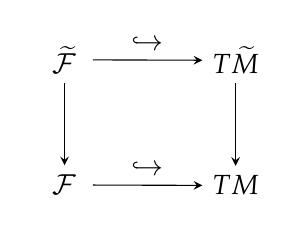
\begin{tikzpicture}
 	\matrix (m) [matrix of math nodes,row sep=3em,column sep=4em,minimum width=2em]
 	{
 		\widetilde{\mathcal F} &    T\widetilde{M} \\
 		\mathcal F	& TM    \\};
 	\path[-stealth]
 	(m-1-1) edge node [above] {$\hookto$} (m-1-2)
 	(m-1-1) edge node [right] {} (m-2-1)
 	(m-1-2) edge node [right] {} (m-2-2)
 	(m-2-1) edge node [above] {$\hookto$}  (m-2-2);
 	
 	\end{tikzpicture}
 	\newline
 	then $\widetilde{\mathcal F}$ is integrable.
 	
 	\begin{definition}\label{fol_cov_defn}
 		In the above situation we say that a foliation $\left(\widetilde{M},~ \widetilde{\mathcal F} \right)$ is the \textit{induced by} $p$ \textit{covering} of $\left(M,\mathcal F \right)$ or the $p$-\textit{lift} of $\left(M,\mathcal F \right)$. 
 	\end{definition}
\begin{remark}
 		The $p$-lift of a foliation is described in  \cite{ouchi:cov_fol, xiaolu:foli_cov}.
 	\end{remark}
 \begin{empt}
 	If $\gamma: \left[0,1\right]\to M$ is a path which corresponds to an element of the holonomy groupoid then we denote by $\left[\gamma\right]$ its equivalence class, i.e. element of groupoid.
 	There is the space of half densities $\Omega_{\widetilde{M}}^{1/2}$ on $\widetilde{M}$ which is a lift  the space of half densities $\Omega_{M}^{1/2}$ on $M$. If $L$ is a leaf of $\left(M,\mathcal F \right)$, $L'=\pi^{-1}\left( L\right)$   then a space $\widetilde{L}$ of holonomy covering of  $L$ coincides with the space of the holonomy covering of $L'$. It turns out that $L^2\left( \widetilde{\mathcal G}_{\widetilde{x}}\right)\approx L^2\left(\mathcal G_{ \pi\left(\widetilde{x}\right)} \right)$ for any $\widetilde{x} \in \widetilde{M}$.
 	If $\mathcal G$ (resp. $\widetilde{\mathcal G}$) is a holonomy groupoid of $\left(M,\mathcal F \right)$ (resp. $\left(\widetilde{M},~ \widetilde{\mathcal F} \right)$) then there is the surjective map $p_{\mathcal G}:\widetilde{\mathcal G} \to \mathcal G$ given by
 	\begin{equation*}
 	\begin{split}
 	\left[\widetilde{\gamma}\right] \mapsto \left[p \circ\widetilde{\gamma}\right]
 	\end{split}
 	\end{equation*}
 	If the covering is finite-fold then the map $p_{\mathcal G}:\widetilde{\mathcal G} \to \mathcal G$ induces 
 	a natural involutive homomorphism
 	\begin{equation*}
 	\begin{split}
 	\Coo_c\left(\mathcal G,  \Omega_{M}^{1/2}\right) \hookto  \Coo_c\left(\widetilde{\mathcal G},  \Omega_{\widetilde{M}}^{1/2}\right)
 	\end{split}
 	\end{equation*}	
 	Completions of $\Coo_c\left(\mathcal G,  \Omega_{M}^{1/2}\right)$ and $\Coo_c\left(\widetilde{\mathcal G},  \Omega_{\widetilde{M}}^{1/2}\right)$ with respect to given by \eqref{fol_norm_eqn} norms gives an injective *- homomorphism 
 	\be\label{foli_inc_eqn}
 	\pi: C^*_r\left( M,\mathcal F\right) \hookto C^*_r\left(\widetilde{M},~ \widetilde{\mathcal F} \right)
 	\ee
 	 of $C^*$-algebras. The action of the group $G\left( \left.\widetilde{M}~\right|M\right)$ of covering transformations on $\widetilde{M}$ naturally induces an action of $G\left( \left.\widetilde{M}~\right|M\right)$ on $\left(\widetilde{M},~ \widetilde{\mathcal F} \right)$.  It follows that there is the natural action   $C^*_r\left(\widetilde{M},~ \widetilde{\mathcal F} \right)$ such that 
 	\be\label{foli_exp_g_eqn}
 	C^*_r\left( M, \mathcal{F}\right)   = C^*_r\left(\widetilde{M},~ \widetilde{\mathcal F} \right)^{G\left( \left.\widetilde{M}~\right|M\right)}
 	\ee
 \end{empt}

 	Let $\G\left({M},~ {\mathcal F} \right)$ and $\G\left(\widetilde{M},~ \widetilde{\mathcal F} \right)$ be the holonomy groupoids of $\left({M},~ {\mathcal F} \right)$ and $\left(\widetilde{M},~ \widetilde{\mathcal F} \right)$ respectively. The natural surjective map $\G\left(\widetilde{M},~ \widetilde{\mathcal F} \right)\to\G\left({M},~ {\mathcal F} \right)$ induces the injective *-homomorphism $C_r^*\left(\widetilde{M},~ \widetilde{\mathcal F} \right)\hookto C^*_r\left(\widetilde{M},~ \widetilde{\mathcal F} \right)$.
 	Assume both $\G\left({M},~ {\mathcal F} \right)$ and $\G\left(\widetilde{M},~ \widetilde{\mathcal F} \right)$ are Hausdorff. Let $G\left( \left.\widetilde{M}~\right|M\right)$  be the covering 	group of  $p:\widetilde M \to M$ . The $G\left( \left.\widetilde{M}~\right|M\right)$-action on $\widetilde{M}$ can be naturally extended to $\G\left(\widetilde{M},~ \widetilde{\mathcal F} \right)$ by sending $\widetilde{\ga}$ to $g\widetilde{\ga}$ for a representative path $\widetilde{\ga}$ in $ \widetilde{M}$ and $g \in G\left( \left.\widetilde{M}~\right|M\right)$. %Therefore we have a transformation groupoid $G\left( \left.\widetilde{M}~\right|M\right)\times \G\left(\widetilde{M},~ \widetilde{\mathcal F} \right)$, with the composition law $\left(g',g\widetilde{\ga} \right)\left(g, \widetilde{\ga}\right) =  \left(g'g, \widetilde{\ga}\right)$.  	 Let $G = \G\left({M},~ {\mathcal F} \right)$, $H = G\left( \left.\widetilde{M}~\right|M\right)\times \G\left(\widetilde{M},~ \widetilde{\mathcal F} \right)$, and $Z = \G\left(\widetilde{M},~ \widetilde{\mathcal F} \right)$. Clearly, the  		unit spaces are $G^0 = M$ and $H^0 = M$. Define $\rho: Z \to G^0$ and $\sigma: Z \to H^0$ by $\rho\left(\widetilde{\ga}\right)= p\left(r\left(\widetilde{\ga} \right)  \right)$  $\sigma\left( \widetilde{\ga}\right) = p\left(r\left( \widetilde{\ga}\right)  \right)$. Both are continuous open maps. The space $Z$ is
 	\begin{lemma}\cite{xiaolu:foli_cov}
 	Let $p:\widetilde M \to M$ be a regular covering manifold with covering group $G\left( \left.\widetilde{M}~\right|M\right)$
 	$N\subset M$ a connected submanifold, and $\widetilde N$ a connected component of $p^{-1}\left( N\right) $
 	Then the restriction $p_{\widetilde N}$ of $p$ to $N$ is also regular, with the covering group $G\left( \left.\widetilde{N}~\right|N\right)$ being a  	subgroup  $G\left( \left.\widetilde{M}~\right|M\right)$.
 	\end{lemma}
 In particular, if $L_{\widetilde x}$ is the leave in $\left(\widetilde{M},~ \widetilde{\mathcal F} \right)$ containing $\widetilde x \in p^{-1}\left( x\right)$ , where $x \in M$,
 then $L_{\widetilde x}$ is a regular cover of $L_x$. We denote the covering group by $G\left( \left.\widetilde{M}~\right|M\right)_x$. On the  other hand, for each $x \in M$, there is a holonomy group $\G^x_x$, and we have the holonomy group bundle $\left\{\G^x_x\right\}$ over $M$. If $x_1$, $x_2$ are on the same leaf, then any path $\ga$  connecting $x_1$ and $x_2$ induces an isomorphism $\ga^*: \G^{x_1}_{x_1}\xrightarrow{\cong}\G^{x_2}_{x_2}$  by mapping $\left[\ga_1\right]$ to $\left[\ga\ga_1\ga^{-1}\right]$.
As a local homeomorphism, the covering map $p$ induces an embedding $\overline{p} : \G^{\widetilde x}_{\widetilde x}\to \G^x_x$ for each $\widetilde x \in p^{-1}\left( x\right)$.
\begin{lemma}\cite{xiaolu:foli_cov}
The group $\overline{p}^*_x\left(\G^{\widetilde x}_{\widetilde x}\right)$ is a normal subgroup of $G^x_x$. Equivalently,
$\overline{p}^*_x\left( \G^{\widetilde x_1}_{\widetilde x_1}\right) =\overline{p}^*_x\left( \G^{\widetilde x_2}_{\widetilde x_2}\right)$ for $\widetilde x_1, \widetilde x_2 \in p^{-1}\left(x\right)$ if $L_{\widetilde x_1}=L_{\widetilde x_2}$,
\end{lemma}
Thus we may form the quotient holonomy group bundle $\left\{\G^{\widetilde x}_{\widetilde x}\right\}$ over $M$. There is an obvious group homomorphism $\phi_x: G\left( \left.\widetilde{M}~\right|M\right)_x \to \G^{ x}_{ x}/\G^{\widetilde x}_{\widetilde x}$ defined as follows. An element $g\in G\left( \left.\widetilde{M}~\right|M\right)_x$ corresponds to a point $x_g \in p^{-1}\left( x\right)\cap L_{\widetilde x}$ if we fix $\widetilde x$ corresponding
to the unit $e$. A path $\ga_g$ starting at  $\widetilde x$ and ending at $g \widetilde x$ gives a loop $\pi\left(\widetilde \ga_g \right)$  in $M$ representing an element $\phi_x\left(g \right)$  in $G_x$, whose class in $\G^{ x}_{ x}/\G^{\widetilde x}_{\widetilde x}$ is uniquely defined
	by $g$. Given any $\left[\ga\right]$ in $\G^{ x}_{ x}$ there is a preimage $\widetilde \ga$ in $L_{\widetilde x}$ starting at $\widetilde x$. The point $r\left( \widetilde \ga\right) \in p^{-1}\left( x\right)\cap  L_{\widetilde x}$ corresponding to some $g\in G\left( \left.\widetilde{M}~\right|M\right)_x$. So $\phi_x$ is onto.
	\begin{definition}\cite{xiaolu:foli_cov}\label{foli_reg_cov_defn}
		The covering map $p:\left(\widetilde{M},~ \widetilde{\mathcal F} \right)\to\left({M},~ {\mathcal F} \right)$ of foliations is said to be \textit{regular} if the map $\phi$ is an isomorphism from the leaf covering group bundle to the quotient holonomy group bundle.
	\end{definition}

\begin{remark}\label{foli_action_rem}
Every regular covering map $p:\left(\widetilde{M},~ \widetilde{\mathcal F} \right)\to\left({M},~ {\mathcal F} \right)$ of foliations induces nontrivial action of $G\left( \left.\widetilde{M}~\right|M\right)$ on $C^*_r\left(\widetilde{M},~ \widetilde{\mathcal F}  \right)$ such that $$C^*_r\left(\widetilde{M},~ \widetilde{\mathcal F}  \right)^{ G\left( \left.\widetilde{M}~\right|M\right)}\cong C^*_r\left(\widetilde{M},~ \widetilde{\mathcal F}  \right).$$
\end{remark}
\begin{remark}\label{foli_trans_rem}
If a map $p:\left(\widetilde{M},~ \widetilde{\mathcal F} \right)\to\left({M},~ {\mathcal F} \right)$ is regular covering of foliations  and a leaf $\widetilde L \in \widetilde M$ has no holonomy then  $g\widetilde L \neq \widetilde L$ for all nontrivial $g \in G\left( \left.\widetilde{M}~\right|M\right)$, i.e. $G\left( \left.\widetilde{M}~\right|M\right)$ transitively acts on leaves having no holonomy.
\end{remark}


 	\chapter{Miscellany}
 		\section{Pre-order category}
 	\begin{definition}\label{preordercat_defn}\cite{goldblatt:topoi}
 		A category is said to be a \textit{pre-order category} if there is at most one morphism between different objects.
 	\end{definition}
 	\begin{definition}
 		A binary relation $R \subset \La\times \La$ on the set $\La$ (writing $pRq$ in place of $\left(p,q \right)\in R$ ) is said to be \textit{pre-ordering} if it is 
 		\begin{enumerate}
 			\item [(a)] \textit{reflexive}, i.e. for each $p$ we have $pRp$ and
 			\item[(b)] \textit{transitive}, whenever $pRq$ and $qRs$, we have $pRs$.
 		\end{enumerate}
 	\end{definition}
 	\begin{remark}\label{pre_order_rem}
 		For any set $\La$ with pre-ordering $R$ there is a pre-order category such that
 		\begin{enumerate}
 			\item [(a)] Objects of the category are elements of $\La$.
 			\item[(b)] Morphisms are pairs $\left(p, q \right) \in R$.
 			\item[(c)] The composition of morphisms is given by $\left(q,s\right)\circ \left(p, q\right) =\left(p,s\right)$.
 		\end{enumerate}
 		
 	\end{remark}
 	
 \section{Flat connections in the differential geometry}\label{geom_flat_subsec}
 \paragraph*{}
 Here I follow to \cite{koba_nomi:fgd}. Let $M$ be a manifold and $G$ a Lie group. A (\textit{differentiable}) \textit{principal bundle over M with group} $G$ consists of a manifolfd $P$ and an action of $G$ on $P$ satisfying the following conditions:
 \begin{enumerate}
 	\item [(a)] $G$ acts freely on $P$ on the right: $\left(u, a \right) \in P \times G \mapsto ua = R_au \in P$;
 	\item[(b)] $M$ is the quotient space of $P$ by the equivalence relation induced by $G$, i.e. $M = P/G$, and the canonical projection $\pi: P \to M$ is differentiable;
 	\item[(c)] $P$ is locally trivial, that is, every point $x$ of $M$ has an open neighborhood $U$ such that $\pi^{-1}\left( U\right)$ is isomophic to  $U\times G$ in the sense that there is a diffeomorphism $\psi:  \pi^{-1}\left( U\right) \to U \times G$ such that $\psi\left( u\right) = \left( \pi\left( u\right), \varphi\left(u \right) \right) $ where $\varphi$ is a mapping of $\pi^{-1}\left(U \right)$ into $G$ satisfying  $\psi\left(ua \right)= \left( \psi\left( u\right)\right) a$  for all $u \in \pi^{-1}\left(U \right)$ and $a \in G$. 
 \end{enumerate}
 A principal fibre bundle will be denoted by $P\left( M, G, \pi\right), ~ P\left(M, G \right)$ or simply $P$.
 \paragraph*{} Let $P\left(M, G \right)$ be a principal fibre bundle over a manifold with group $G$. For each $u \in P$ let $T_u\left(P \right)$ be a tangent space of $P$ at $u$ and $G_u$ the subspace of $T_u\left( P\right)$ consisting of vectors tangent to the fibre through $u$. A \textit{connection} $\Ga$   in $P$ is an assignment of a subspace $Q_u$ of $T_u\left(P \right)$ to each $u \in P$ such that
 \begin{enumerate}
 	\item [(a)] $T_u\left(P \right) = G_u \oplus Q_u$ (direct sum);
 	\item[(b)] $Q_{ua}= \left(R_a \right)_*Q_u$ for every $u \in P$ and $a \in G$, where $R_a$ is a transformation of $P$ induced by $a \in G, ~ R_au=ua$.
 \end{enumerate}
 \paragraph*{}
 Let $P = M \times G$ be a trivial principal bundle. For each $a \in G$, the set $M \times \{a\}$ is a submanifold of $P$. The \text{canonical flat connection} in $P$ is defined by taking the tangent space to $M \times \{a\}$ at $u = \left(x, a \right)$ as the horizontal tangent subspace at $u$. A connection in any principal bundle is called \textit{flat} if every point has a neighborhood such that the induced connection in $P|_U = \pi^{-1}\left(U \right)$ is isomorphic with the canonical flat connection.
 \begin{cor}\label{dg_flat_cor}(Corollary II 9.2 \cite{koba_nomi:fgd})
 	Let $\Ga$ be a connection in $P\left(M, G \right)$ such that the curvature vanishes identically. If $M$ is paracompact and simply connected, then $P$ is isomorphic to the trivial bundle and $\Ga$ is isomorphic to the canonical flat connection in $M \times G$.
 \end{cor}
 \paragraph*{}
 
 If $\widetilde{\pi}: \widetilde{M} \to M$ is a covering then the $\widetilde{\pi}$-\textit{lift} of $P$ is a principal $\widetilde{P}\left(\widetilde{M}, G \right)$  bundle, given by
 \be\nonumber
 \widetilde{P} = \left\{\left(u, \widetilde{x}\right) \in P \times \widetilde{M}~|~ \pi\left(u \right) = \widetilde{\pi}\left( \widetilde{x}\right) \right\}.
 \ee
 If $\Ga$ is a  connection on $P\left( M, G\right)$ and $\widetilde{M} \to M$ is a covering then is a canonical connection $\widetilde{\Ga}$ on $\widetilde{P}\left(\widetilde{M}, G \right)$ which is the \textit{lift} of $\Ga$, that is, for any $\widetilde{u} \in \widetilde{P}$ the horizontal space $\widetilde{Q}_{\widetilde{u}}$ is isomorphically  mapped onto the horizontal space $Q_{\widetilde{\pi}\left(\widetilde{u} \right) }$ associated with the connection $\Ga$.
 If $\Ga$ is flat then from the Proposition (II 9.3 \cite{koba_nomi:fgd}) it turns out that there is a covering $\widetilde{M} \to M$ such that $\widetilde{P}\left(\widetilde{M}, G \right)$ (which is the lift of $P\left(M,G\right)$) is a trivial bundle, so the lift $\widetilde{\Ga}$ of $\Ga$ is a canonical flat connection (cf. Corollary \ref{dg_flat_cor}). From the the Proposition (II 9.3 \cite{koba_nomi:fgd}) it follows that for any flat connection $\Ga$  on $P\left(M, G \right)$ there is a group homomorphism $\varphi: G\left( \widetilde{M} ~|~ M\right) \to G$ such that
 \begin{enumerate}
 	\item [(a)] There is an action $G\left( \widetilde{M} ~|~ M\right) \times \widetilde{P} \to \widetilde{P} \approx \widetilde{M} \times G$ given by
 	$$
 	g \left(\widetilde{x}, a \right) = \left( g\widetilde{x}, \varphi\left( g\right) a\right); \forall \widetilde{x} \in \widetilde{M}, ~ a \in G, 
 	$$
 	\item[(b)] There is the canonical diffeomorphism  $P = \widetilde{P}/G\left( \widetilde{M} ~|~ M\right)$,
 	\item[(c)] The lift $\tilde{\Ga}$ of $\Ga$ is a canonical flat connection.
 \end{enumerate}
 
 \begin{defn}
 	In the above situation we say that the flat connection $\Ga$ is \textit{induced} by the covering $\widetilde{M}\to M$ and the homomorphism $G\left( \left.\widetilde{M}~\right|M\right) \to G$, or we say that $\Ga$ \textit{comes from} $G\left( \left.\widetilde{M}~\right|M\right) \to G$.
 \end{defn}
 \begin{remark}
 	The  Proposition (II 9.3 \cite{koba_nomi:fgd}) assumes that $\widetilde{M} \to M$ is the universal covering however it is not always necessary requirement.
 \end{remark}
 \begin{remark}
 	If $\pi_1\left(M, x_0 \right)$ is the fundamental group \cite{spanier:at} then there is the canonical surjective homomorphism $\pi_1\left(M, x_0 \right) \to G\left( \left.\widetilde{M}~\right|M\right)$. So there exist the composition $\pi_1\left(M, x_0 \right) \to G\left( \left.\widetilde{M}~\right|M\right) \to G$. It follows that any flat connection comes from the homomorphisms $\pi_1\left(M, x_0 \right) \to G$. 
 \end{remark} 
 \paragraph*{}
 Suppose that there is the right action of $G$ on $P$ and suppose that $F$ is a manifold with the left action of $G$. There is an action of $G$ on $P \times F$ given by $a\left( u, \xi\right) = \left(u a, a^{-1}\xi \right)$ for any $a \in G$ and $\left( u, \xi\right) \in P\times F$. The quotient space $P \times_G F = \left(P \times F \right)/G$ has the natural structure of a manifold and if $E =  P \times_G F$ then $E\left(M, F, G, P \right)$ is said to be the \textit{fibre bundle over the base $M$, with (standard) fibre $F$, and (structure) group G which is associated with the principal bundle P} (cf. \cite{koba_nomi:fgd}). If $P = M \times G$ is the trivial bundle then $E$ is also trivial, that is, $E = M \times F$. If $F = \C^n$ is a vector space and the action of $G$ on $\C^n$ is a linear representation of the group then $E$ is the linear bundle. Denote by $T\left(M \right)$ (resp. $T^*\left(M \right)$) the tangent  (resp. contangent) bundle, and denote by $\Ga\left( E\right)$, $\Ga\left(T\left(M \right)\right)$, $\Ga\left(T^*\left(M \right)\right)$ the spaces of sections of $E$, $T\left(M \right)$, $T^*\left(M \right)$ respectively. Any connection $\Ga$ on $P$ gives a covariant derivative  on $E$, that is,
 for any section  $X \in \Ga\left( T\left(M \right)\right) $ and any section $\xi \in \Ga\left( E\right)$ there is the derivative given by
 \be\nonumber
 \nabla_X\left( \xi\right) \in \Ga\left( E\right).
 \ee
 If $E = M \times \C^n$, $\Ga$ is the canonical flat connection and $\xi$ is a trivial section, that is, $\xi = M \times \{x\}$ then 
 \be\label{comm_triv_eqn}
 \nabla_X \xi = 0,~~ \forall X \in T\left(M \right).
 \ee
 For any connection there is the unique map
 \be\label{comm_alg_conn}
 \nabla : \Ga\left( E\right) \to \Ga\left( E \otimes T^*\left( M\right) \right)
 \ee
 such that
 \be\nonumber
 \nabla_X \xi = \left(\nabla \xi, X \right)
 \ee
 where the pairing $\left(\cdot, \cdot\right) : \Ga\left( E \otimes T^*\left( M\right) \right) \times \Ga\left( T\left( M\right)\right)  \to \Ga\left( E \right) $ is induced by the pairing $\Ga\left( T^*\left(M \right)\right)   \times \Ga\left( T\left( M\right)\right)  \to \Coo\left(M \right) $.
 
 \section{Quantum $SU\left(2 \right)$ and $SO\left(3 \right)$}
 \paragraph*{}
 There is a quantum generalization of $SU\left(2 \right)$ and  we will introduce a quantum analog of $SO\left(3 \right)$.
 Let $q$ be a real number such that $0<q<1$. 
 A quantum group $C\left( \SU_q(2)\right) $ is the universal $C^*$-algebra algebra generated by two elements $\al$ and $\beta$ satisfying the following relations:
 \begin{equation}\label{su_q_2_rel_eqn}
 \begin{split}
 \al^*\al + \beta^*\beta = 1, ~~ \al\al^* + q^2\beta\beta^* =1,
 \\
 \al\bt - q \bt\al = 0, ~~\al\bt^*-q\bt^*\al = 0,
 \\
 \bt^*\bt = \bt\bt^*.
 \end{split}
 \end{equation}
 From  $C\left( SU_1\left(2 \right)\right) \approx C\left(SU\left(2 \right)  \right)$ it follows that  $C\left( \SU_q(2)\right) $ can be regarded as a noncommutative deformation of the space $SU(2)$. 
 The dense pre-$C^*$-algebra $\Coo\left( SU_q(2)\right) \subset C\left( SU_q(2)\right)$ is defined in  \cite{chakraborty_pal:quantum_su_2}. 
 Let $Q, S \in B\left( \ell_2\left(\N^0 \right)\right) $ be given by 
 \begin{equation*}
 \begin{split}
 Qe_k= q^ke_k, \\
 Se_k = \left\{
 \begin{array}{c l}
 e_{k-1} & k > 0 \\
 0 & k = 0
 \end{array}\right..
 \end{split}
 \end{equation*}
 and let $R \in B\left( \ell_2\left(\Z \right)\right) $ be given by $e_k \mapsto e_{k+1}$.
 There is a faithful representation \cite{woronowicz:su2}  $C\left(\SU_q\left( 2\right) \right) \to B\left(\ell_2\left(\N^0 \right) \otimes \ell_2\left(\Z \right) \right)  $ given by
 
 \begin{equation}\label{su_q_2_repr_eqn}
 \begin{split}
 \al \mapsto S\sqrt{1 - Q^2} \otimes 1, \\
 \bt \mapsto Q \otimes R.
 \end{split}
 \end{equation}
  There is a faithful state $h:C\left( SU_q(2)\right) \to \C$ given by
 \be\label{su_q_2_haar_eqn}
 h\left(a \right)  = \sum_{n = 0}^\infty q^{2n}\left(e_n \otimes e_0, a  e_n \otimes e_0\right) 
 \ee
 where $a \in C\left( SU_q(2)\right)$ and $e_0 \otimes e_n \in \ell_2\left(\N^0 \right) \otimes \ell_2\left(\Z \right)$ (cf. \cite{woronowicz:su2}).
 \begin{defn}
 	The state $h$ is said to be the \textit{Haar measure}.
 \end{defn}
 
 Denote by $L^2\left( C\left( SU_q\left(2\right)\right), h\right) $ the GNS space associated with the state $h$. 
 The representation theory of $SU_q(2)$ is strikingly similar to its
 classical counterpart.  In particular, for each $l\in\{0,\frac{1}{2},
 1,\ldots\}$, there is a unique irreducible unitary representation
 $t^{(l)}$ of dimension $2n+1$.  Denote by $t^{(l)}_{jk}$ the
 $jk$\raisebox{.4ex}{th} entry of $t^{(l)}$. These are all elements of
 $\A_f$ and they form an orthogonal basis for $L^2\left( C\left( SU_q\left(2\right)\right), h\right)$. Denote by
 $e^{(l)}_{jk}$ the normalized $t^{(l)}_{jk}$'s, so that
 $\{e^{(l)}_{jk}: n=0,\frac{1}{2},1,\ldots, i,j=-n,-n+1,\ldots, n\}$ is
 an orthonormal basis. The definition of equivariant operators (with respect to action of quantum groups) is described in \cite{chakraborty_pal:inv_hom}. It is proven in \cite{chakraborty_pal:quantum_su_2} that any unbounded equivariant operator $\widetilde{D}$ satisfies to the following condition
 \be \label{su_q_2_dirac_eqn}
 \widetilde{D}: e^{(l)}_{jk}\mapsto d(l,j)e^{(l)}_{jk},
 \ee
 Moreover if
 \be \label{su_q_2_genericd_eqn}
 d(l,j)=\begin{cases}2l+1 &  l \neq j,\cr
 	-(2l+1) & l=j,\end{cases}
 \ee
 
 then there is a 3-summable spectral triple 
 \be \label{su_q_2_spt_eqn}
 \left(\Coo\left( SU_q\left(2\right)\right), L^2\left( C\left( SU_q\left(2\right)\right), h\right), \widetilde{D} \right) 
 \ee
 described in \cite{chakraborty_pal:quantum_su_2}. 
 
 According to \cite{kl-sch} (equations (4.40)-(4.44) ) following condition holds
 \begin{equation}\label{su_q_2_tij_eqn}
 \begin{split}
 t^{\left(l \right) }_{jk}= M^l_{jk} \al^{-j-k}\bt^{k-j}p_{l + k}\left( \bt\bt^*; q^{-2\left(k-j \right) }q^{2\left(j + k \right)}~|~q^2 \right); ~~ j + k \le 0 ~\&~ k \ge j,
 \\ 
 t^{\left(l \right) }_{jk}= M^l_{jk} \al^{-j-k}\bt^{*\left( k-j\right) }p_{l + k}\left( \bt\bt^*; q^{-2\left(k-j \right) }q^{2\left(j + k \right)}~|~q^2 \right); ~~ j + k \le 0 ~\&~ k \le j,
\\ 
 t^{\left(l \right) }_{jk}= M^l_{j,k}p_{l - k}\left( \bt\bt^*; q^{-2\left(k-j \right) }q^{2\left(j + k \right)}~|~q^2 \right)\bt^{k-j}\al^{*j+k}; ~~ j + k \ge 0 ~\&~ k \ge j,\\ 
 t^{\left(l \right) }_{jk}= M^l_{k,j}p_{l - j}\left( \bt\bt^*; q^{-2\left(k-j \right) }q^{2\left(j + k \right)}~|~q^2 \right)\bt^{*j-k}\al^{*j + k}; ~~ j + k \ge 0 ~\&~ j \ge k\\ 
 \end{split}
 \end{equation}
  where $M^l_{jk} \in \R$ for any $l, j, k$ and $p_{l - k}\left( x; q^{-2\left(k-j \right) }q^{2\left(j + k \right)}~|~q^2 \right)$ is little Jacobi polynomial (cf. \cite{kl-sch}).  
 Denote by $g \in \Z_2$ the unique nontrivial element.
 There is a surjective group homomorphism
 $$
 \Phi : SU\left(2 \right) \to SO\left(3 \right) ,~ \ker \Phi = \Z_2 = \{\pm 1\}
 $$
 and the natural action of $\Z_2$ on $SU(2)$ such that
 \be\label{su_q_2_z2_comm_eqn}
 \begin{split}
 	SO\left(3 \right) \cong SU\left(2\right)/\Z_2,\\
 	g\begin{pmatrix} \al & -\overline{\bt}\\
 		\bt & \overline{\al}\end{pmatrix}= \begin{pmatrix} -\al & \overline{\bt}\\
 		-\bt & -\overline{\al}\end{pmatrix};~ \forall \begin{pmatrix} \al & -\overline{\bt}\\
 		\bt & \overline{\al}\end{pmatrix}\in SU\left(2\right).
 \end{split}
 \ee	
 This action induces an action of $\Z_2$  on a $C^*$-algebra $C\left(SU\left(2\right) \right)$ given by
 \be\nonumber
 \begin{split}
 	g\al = -\al, ~~ g\bt = - \bt
 \end{split}
 \ee
 where $\al, \bt$ are regarded as functions $\SU\left(2 \right) \to \C$.
 Indeed 	$ SU\left(2 \right)$ is an oriented manifold, $SO\left(3 \right)$ is an unoriented one, and $ SU\left(2 \right) \to SO\left(3 \right)$ is a two-fold covering
 There is a quantum generalization of $SU\left(2 \right)$ and  we will introduce a quantum analog of $SO\left(3 \right)$.
 Let $q$ be a real number such that $0<q<1$. 
There is a noncommutative analog of the action \eqref{su_q_2_z2_comm_eqn} described in \cite{dijkhuizen:so_doublecov,lance:so,podles:so_su}
\begin{equation}\label{su_q_2_z2_ncomm_eqn}
\begin{split}
\Z_2 \times C\left( SU_q\left(2\right)\right)\to C\left( SU_q\left(2\right)\right),\\
g\al = -\al,~g \bt = -\bt.
\end{split}
\end{equation} 
In \cite{dijkhuizen:so_doublecov,lance:so,podles:so_su} the quantum group 	$SO_q\left(3 \right)$ is defined, moreover in 
it is proven in \cite{dijkhuizen:so_doublecov,podles:so_su} following 
$$
	C\left( 	SO_q\left(3 \right) \right) \stackrel{\mathrm{def}}{=} C\left( SU_q\left(2\right)\right) ^{\Z_2}\cong \left\{\widetilde{a}\in C\left( SU_q\left(2\right)\right) ,~ g\widetilde{a} = \widetilde{a} \right\}.
$$
Above equation can be used as the definition of $SO_q\left(3 \right)$
 \begin{definition}\label{su_q_2_so3_defn}
	Denote by
	\begin{equation}\label{su_q_2_so3_eqn}
	C\left( 	SO_q\left(3 \right) \right) \stackrel{\mathrm{def}}{=} C\left( SU_q\left(2\right)\right) ^{\Z_2}\cong \left\{\widetilde{a}\in C\left( SU_q\left(2\right)\right) ,~ g\widetilde{a} = \widetilde{a} \right\}.
	\end{equation}
	The $C^*$-algebra $C\left( 	SO_q\left(3 \right)\right) $ is said to be the \textit{quantum 	$ SO\left(3 \right)$}.
\end{definition}
\begin{remark}
	Our definition of $SO_q\left(3 \right)$  differs from the Definition given in other sources. For example the quantum group defined in \cite{rtf:qlie} is a
	quantization of $O\left( 3\right)$  and not of $SO(3)$ (cf. \cite{dijkhuizen:so_doublecov}). 
\end{remark}

 \begin{thm}\label{su_q_2_bas_thm}\cite{woronowicz:su2}
 	Let  $q \neq 0$, and let $\A_f$ the dense involutive subalgebra of $C\left( SU_q(2)\right)$ generated  by $\alpha, \beta$. The set of elements of the form
 	\be\label{su_q_2_fin_eqn}
 	\al^k\bt^n\bt^{*m}~~ \text{ and }~~ \al^{*k'}\bt^n\bt^{*m}
 	\ee 
 	where $k, m, n = 0, \dots;~k'=1, 2,\dots$ forms a basis in $\A_f$: any element
 	of $\A_f$ can be written in the unique way as a finite linear combination of
 	elements of \eqref{su_q_2_fin_eqn}.
 \end{thm}
\section{Presheaves and Sheaves}

\begin{definition}\label{presheaf_defn}\cite{hartshorne:ag}
Let $\sX$ be a topological space. A \textit{presheaf} $\mathscr F$ of Abelian groups on  $\sX$ consists of the data
\begin{itemize}
	\item[(a)] for every open subset $\sU \subseteq \sX$, an Abelian group $\mathscr F\left(\sU\right)$, and 
	\item[(b)] for every inclusion $\sV \subseteq \sU$ of open subsets of $\sX$, a morphism of Abelian groups $\rho_{\sU \sV}:\mathscr F\left(\sU\right) \to \mathscr F\left(\sV\right)$,\\
	subject to conditions
	\begin{itemize}
		\item [(0)] $\mathscr F\left(\sV\right)= 0$, where $\emptyset$ is the empty set,
		\item[(1)] $\rho_{\sU \sU}$ is the identity map, and
		\item[(2)] if $\mathcal W \subseteq \sV \subseteq \sU$ are three open sets, then $\rho_{\sU \mathcal W} = \rho_{\sV \mathcal W }\circ \rho_{\sU \sV}$.
	\end{itemize}
\end{itemize}
\end{definition}

\begin{definition}\label{sheaf_defn}\cite{hartshorne:ag}
	 A \textit{presheaf} $\mathscr F$ on a 
 a topological space $\sX$ is a \textit{sheaf}  if it satisfies the following supplementary conditions:
	\begin{itemize}
		\item[(3)] If $\sU$ is an open set, if $\left\{\sV_{\a}\right\}$ is an open covering of $\sU$, and if $s \in \mathscr F\left(\sU\right)$ is an element such that $\left.s\right|_{\sV_{\a}}= 0$ for all $\a$, then $s = 0$;
		\item[(4)] If $\sU$ is an open set, if $\left\{\sV_{\a}\right\}$ is an open covering of $\sU$, and we have elements $s_\a$ for each $\a$, with property that for each $\al, \bt, \left.s_\a\right|_{\sV_{\a}\cap \sV_{\bt}}= \left.s_\a\right|_{\sV_{\bt}\cap \sV_{\bt}}$, then there is an element $s \in  F\left(\sV\right)$ such that $\left.s\right|_{\sV_\a} = s_\a$ for each $\a$.
	\end{itemize}
(Note condition (3) implies that $s$ is unique.)
\end{definition}
%\begin{definition}
%	A presheaf satisfying (4) of the Definition \ref{sheaf_defn} is called \textit{conjunctive} (for $\sU$). (cf. \cite{bredon:sheaf})
%\end{definition}

\begin{definition}\label{stalk_defn}\cite{hartshorne:ag}
	If $\mathscr F$ is a {presheaf} on $\sX$, and if $x$ is a point of $\sX$ we define the \textit{stalk} $\mathscr F_x$ of $\mathscr F$ at $x$ to be the direct limit of groups $\mathscr F\left(\sU\right)$ for all open sets $\sU$ containing $x$, via restriction maps $\rho$.
	\end{definition}

\begin{prdf}\label{sheaf_prdf}\cite{hartshorne:ag}
	Given a presheaf $\mathscr F$, there is a sheaf $\mathscr F^+$ and a morphism $\th: \mathscr F \to \mathscr F^+$, with the property that for any sheaf $\mathscr G$, and any morphism $\varphi: \mathscr F \to \mathscr G$, there is a unique morphism $\psi:\mathscr F^+\to \mathscr G$ such that $\varphi = \psi \circ \th$. Furthermore the pair $\left(\mathscr F^+, \th\right)$ is unique up to unique isomorphism. $\mathscr F^+$ is called the $\mathrm{sheaf~associated}$ to the preseaf $\mathscr F$. 
\end{prdf}
\begin{empt}\label{sheaf_empt}
Following text is the citation of the proof of \ref{sheaf_prdf} (cf. \cite{hartshorne:ag}). For any open set $\sU$, let $\mathscr F^+\left(\sU\right)$ be set of functions $s$ from $\sU$ to the union $\bigcup_{x \in \sU}  \mathscr F_x$ of stalks of $\mathscr F$ over points of $\sU$, such that
\begin{itemize}
	\item [(1)] for each $x \in \sU$, $s\left(x\right)\in \mathscr F_x$, and
	\item[(2)] for each $x \in \sU$, there is a neighborhood $\sV$ of $x$ contained in $\sU$ and an element $t \in \mathscr F\left(\sV\right)$, such that for all $y \in \sV$ the germ $t_y$ of $t$ at $y$ is equal to $s\left(y\right)$.
\end{itemize}
\end{empt}
\begin{definition}\label{sheaf_inv_im_defn}\cite{hartshorne:ag}
	Let $f: \sX\to \sY$ be a continuous map of topological spaces. For any sheaf $\mathscr F$ on $\sX$, we define the \textit{direct image} sheaf $f_*\mathscr F$ on $\sY$ by $\left(f_*\mathscr F\right)\left(\sV\right)= \mathscr F\left(f^{-1}\left(\sV\right)\right)$ for any open set $\sV \subseteq \sY$. For any sheaf $\mathscr G$ on $\sY$, we define the \textit{inverse image} sheaf $f^{-1}\mathscr G$ on $\sX$ be the sheaf associated to the presheaf $\sU \mapsto \lim_{\sV \supseteq f\left(\sU\right)} \mathscr G\left(\sV\right)$, where $\sU$ is any open set in $\sX$, and the limit is taken over all open sets $\sV$ of $\sV$ containing $f\left(\sU\right)$.
\end{definition}
\begin{definition}\label{sheaf_hom_defn}\cite{hartshorne:ag}
	Let $\mathscr F$, $\mathscr G$ be sheaves of Abelian  groups  on $\sX$. For any open set $\sU \subseteq \sX$ the set of morphisms $\Hom\left(\left.\mathscr F\right|_{\sU}, \left.\mathscr G\right|_{\sU}\right)$ has the natural structure of Abelian group. It is a sheaf (cf. \cite{hartshorne:ag}). It is called the \textit{sheaf of local morphisms} of $\mathscr F\to \mathscr G$, "sheaf hom" for short, and is denoted by $\mathscr Hom \left(\mathscr F, \mathscr G\right)$.
\end{definition}


Recall that for $s \in \mathscr{F}\left(\sX \right)$, $\supp s= \left\{\left.x \in \sX \right|s\left(x \right)\neq 0  \right\}$ denotes the \textit{support} of the section $s$.



\section{Isospectral deformations}
\paragraph*{}A very general construction of isospectral
deformations
of noncommutative geometries is described in \cite{connes_landi:isospectral}. The construction
implies in particular that any
compact Riemannian manifold $M$ which  admits a spin$^c$ structure (cf. Definition \ref{spin_str_defn}), whose isometry group has rank
$\geq 2$ admits a
natural one-parameter isospectral deformation to noncommutative geometries
$M_\theta$.
We let $(\Coo\left(M \right)  , \H = L^2\left(M,S \right)  , \slashed D)$ be the canonical spectral triple associated with a
compact spin-manifold $M$. We recall that $\mathcal{A} = C^\infty(M)$ is
the algebra of smooth
functions on $M$, $S$ is the spinor bundle and $\slashed D$
is the Dirac operator.
Let us assume that the group $\mathrm{Isom}(M)$ of isometries of $M$ has rank
$r\geq2$.
Then, we have an inclusion
\begin{equation}\label{isos_t_act_eqn}
\mathbb{T}^2 \subset \mathrm{Isom}(M) \, ,
\end{equation}
with $\mathbb{T}^2 = \mathbb{R}^2 / 2 \pi \mathbb{Z}^2$ the usual torus, and we let $U(s) , s \in
\mathbb{T}^2$, be
the corresponding unitary operators in $\H = L^2(M,S)$ so that by construction
\begin{equation*}
U(s) \, \slashed D = \slashed D \, U(s).
\end{equation*}
Also,
\begin{equation}\label{isospectral_sym_eqn}
U(s) \, a \, U(s)^{-1} = \alpha_s(a) \, , \, \, \, \forall \, a \in \mathcal{A} \, ,
\end{equation}
where $\alpha_s \in \mathrm{Aut}(\mathcal{A})$ is the action by isometries on the
algebra of functions on
$M$.

\noindent
We let $p = (p_1, p_2)$ be the generator of the two-parameters group $U(s)$
so that
\begin{equation*}
U(s) = \exp(i(s_1 p_1 + s_2 p_2)) \, .
\end{equation*}
The operators $p_1$ and $p_2$ commute with $D$.
Both $p_1$ and $p_2$
have integral spectrum,
\begin{equation*}
\mathrm{Spec}(p_j) \subset \mathbb{Z} \, , \, \, j = 1, 2 \, .
\end{equation*}

\noindent
One defines a bigrading of the algebra of bounded operators in $\H$ with the
operator $T$ declared to be of bidegree
$(n_1,n_2)$ when,
\begin{equation*}
\alpha_s(T) = \exp(i(s_1 n_1 + s_2 n_2)) \, T \, , \, \, \, \forall \, s \in
\mathbb{T}^2 \, ,
\end{equation*}
where $\alpha_s(T) = U(s) \, T \, U(s)^{-1}$ as in \eqref{isospectral_sym_eqn}.
\paragraph{}
Any operator $T$ of class $C^\infty$ relative to $\alpha_s$ (i. e. such that
the map $s \rightarrow \alpha_s(T) $ is of class $C^\infty$ for the
norm topology) can be uniquely
written as a doubly infinite
norm convergent sum of homogeneous elements,
\begin{equation*}
T = \sum_{n_1,n_2} \, \widehat{T}_{n_1,n_2} \, ,
\end{equation*}
with $\widehat{T}_{n_1,n_2}$ of bidegree $(n_1,n_2)$ and where the sequence
of norms $||
\widehat{T}_{n_1,n_2} ||$ is of
rapid decay in $(n_1,n_2)$.
Let $\lambda = \exp(2 \pi i \theta)$. For any operator $T$ in $\H$ of
class $C^\infty$ we define
its left twist $l(T)$ by
\begin{equation}\label{l_defn}
l(T) = \sum_{n_1,n_2} \, \widehat{T}_{n_1,n_2} \, \lambda^{n_2 p_1} \, ,
\end{equation}
and its right twist $r(T)$ by
\begin{equation*}
r(T) = \sum_{n_1,n_2} \, \widehat{T}_{n_1,n_2} \, \lambda^{n_1 p_2} \, ,
\end{equation*}
Since $|\lambda | = 1$ and $p_1$, $p_2$ are self-adjoint, both series
converge in norm. Denote by $\Coo\left(M \right)_{n_1, n_2} \subset \Coo\left(M \right) $ the $\C$-linear subspace of elements of bidegree $\left( n_1, n_2\right) $. \\
One has,
\begin{lem}\label{conn_landi_iso_lem}\cite{connes_landi:isospectral}
	\begin{itemize}
		\item[{\rm a)}] Let $x$ be a homogeneous operator of bidegree $(n_1,n_2)$
		and $y$ be
		a homogeneous operator of  bidegree $(n'_1,n'_2)$. Then,
		\begin{equation}
		l(x) \, r(y) \, - \,  r(y) \, l(x) = (x \, y \, - y \, x) \,
		\lambda^{n'_1 n_2} \lambda^{n_2 p_1 + n'_1 p_2}
		\end{equation}
		In particular, $[l(x), r(y)] = 0$ if $[x, y] = 0$.
		\item[{\rm b)}] Let $x$ and $y$ be homogeneous operators as before and
		define
		\begin{equation*}
		x * y = \lambda^{n'_1 n_2} \, x y \, ; \label{star}
		\end{equation*}
		then $l(x) l(y) = l(x * y)$.
	\end{itemize}
\end{lem}



\noindent
The product $*$ defined in (\ref{star}) extends by linearity
to an associative product on the linear space of smooth operators and could
be called a $*$-product.
One could also define a deformed `right product'. If $x$ is homogeneous of
bidegree
$(n_1,n_2)$ and $y$ is homogeneous of bidegree $(n'_1,n'_2)$ the product is
defined by
\begin{equation*}
x *_{r} y = \lambda^{n_1 n'_2} \, x y \, .
\end{equation*}
Then, along the lines of the previous lemma one shows that $r(x) r(y) = r(x
*_{r} y)$.

We can now define a new spectral triple where both $\H$ and the operator
$\slashed D$ are unchanged while the
algebra $\Coo\left(M \right)$  is modified to $l(\Coo\left(M \right))$ . By
Lemma~{\ref{conn_landi_iso_lem}}~b) one checks that  $l\left( \Coo\left(M \right)\right) $ is still an algebra. Since $\slashed D$ is of bidegree $(0,0)$ one has,
\begin{equation}\label{isospectral_ld_eqn}
[\slashed D, \, l(a) ] = l([\slashed D, \, a]) 
\end{equation}
which is enough to check that $[\slashed D, x]$ is bounded for any $x \in l(\mathcal{A})$. There is a spectral triple $\left(l\left( \Coo\left(M \right)\right) , \H, \slashed D\right)$.
\paragraph{} Denote by $\Coo\left( M_\th\right)$ (resp.  $C\left(M_\th \right)$) the algebra $l\Coo\left( M\right)$ (resp. the operator norm completion of $l\left(\Coo\left( M\right)  \right)  $). Denote by $\rho: C\left(M\right) \to L^2\left( M, S\right) $ (resp. $\pi_\th: C\left(M_\th\right) \to B\left( L^2\left( M, S\right)\right) $ ) natural representations.
%\begin{rem}\label{isosp_grad_rem}
%Indeed there $l: \Coo\left( M\right)  \to \Coo\left( M_{\la}\right) $ is a $\C$-linear isomorphism. The bigrading on $\Coo\left( M\right)$ induces the bigrading $\Coo\left( M_{\la}\right)$.
%\end{rem}
%\begin{empt}
%Denote by $\Ga^\infty\left( M, S\right)$ the space of smooth sections of $S$. Since $M$ is compact any smooth section is square integrable, i.e.
%$$
%\Ga^\infty\left( M, S\right) \subset L^2\left( M, S\right)
%$$ 
%\end{empt}
%and above inclusion is dense. On the other hand for any $n_1, n_2 \in \N$ there is a homogeneous subspace $\Ga^\infty\left( M, S\right)_{n_1,n_2} \subset \Ga^\infty\left( M, S\right)$ given by
%$$
%\Ga^\infty\left( M, S\right)_{n_1,n_2}\left\{\xi \in \Ga^\infty\left( M, S\right)~|~\al_s\left( \xi\right)\exp(i(s_1 n_1 + s_2 n_2))\xi \right\}
%$$
% algebraic direct sum
%$$
%\bigoplus_{n_1,n_1 \in \N } \Ga^\infty\left( M, S\right)_{n_1,n_2}
%$$
%is dense in $L^2\left( M, S\right)$. Otherwise
%$$
%\Coo\left( M\right)_{n'_1,n'_2} \Ga^\infty\left( M, S\right)_{n_1,n_2}\subset \Ga^\infty\left( M, S\right)_{n'_1+n_1,n'_2 + n_2}.
%$$
%From the Remark \ref{isosp_grad_rem} it follows that there is the natural bigrading on $\Coo\left( M_{\la}\right)$. From above construction it turns out
%$$
%\Coo\left( M_{\la}\right)_{n'_1,n'_2} \Ga^\infty\left( M, S\right)_{n_1,n_2}\subset \Ga^\infty\left( M, S\right)_{n'_1+n_1,n'_2 + n_2}.
%$$
%The algebraical direct sum $\bigoplus_{n_1,n_2 \in \N } \Ga^\infty\left( M, S\right)_{n_1,n_2}$ (resp. $\bigoplus_{n_1,n_2 \in \N } \Coo\left( M\right)_{n_1,n_2}$ ) is dense in $L^2\left( M, S\right)$ (resp. $ C\left( M_{\la}\right)$). So the action on $ C\left( M_{\la}\right) \times L^2\left( M, S\right) \to L^2\left( M, S\right)$ can be uniquely defined by the actions of $\Coo\left( M_{\la}\right)_{n'_1,n'_2}$ on $\Ga^\infty\left( M, S\right)_{n_1,n_2}$ for any $n'_1,n'_2, n_1,n_2 \in \N$. 
There is an oriented twisted spectral triple 
\be\label{isos_twisetd_eqn}
\left(l\left( \Coo\left(M \right)\right) , \H, \slashed D\right).
\ee
described in \cite{connes_landi:isospectral}.





 \end{appendices}

 
\begin{thebibliography}{10}


	\bibitem{apt_mult}	Charles A. Akemann, Gert K. Pedersen, Jun Tomiyama. \textit{Multipliers of $C^*$-algebras}. Journal of Functional Analysis Volume 13, Issue 3, July 1973, Pages 277-301, 1973.
	
%\bibitem{akhi:fa}	N. I. Akhiezer, I. M. Glazman. \textit{Theory of Linear Operators in Hilbert Space}. Dover Publications, New York, 1961, 1963.

\bibitem{arveson:c_alg_invt} W. Arveson. {\it An Invitation to $C^*$-Algebras}, Springer-Verlag. ISBN 0-387-90176-0, 1981.
	

\bibitem{atiyah_b_s}
M. F. Atiyah, R. Bott and A. Shapiro, \textit{Clifford Modules}, Topology{\bf 3} (1964), 3--38.  1964.

%\bibitem{ant_azz_scan:flat_k}Paolo Antonini, Sara Azzali, Georges Skandalis {\it Flat bundles, von Neumann algebras and $K$-theory with $\mathbb{R}/\mathbb{Z}$-coefficients}, arXiv:1308.0218, 2013.

\bibitem{auslander:galois} M. Auslander; I. Reiten; S.O. Smal\o{}. \textit{Galois actions on rings and finite Galois coverings}. Mathematica Scandinavica (1989), Volume: 65, Issue: 1, page 5-32, ISSN: 0025-5521; 1903-1807/e , 1989.


%\bibitem{bezandry_diagana:bound_unbound}Paul H. Bezandry, Toka Diagana {\it Bounded and Unbounded Linear Operators}, in {\it Almost Periodic Stochastic Processes}, Springer, 2011.

%\bibitem{ballentine:qm} Leslie E Ballentine. {\it Quantum Mechanics: A Modern Development.} World Scientific Publishing Co. Pte. Ltd. 2000.
\bibitem{bass} H. Bass. {\it Algebraic K-theory.} W.A. Benjamin, Inc. 1968. 

\bibitem{blackadar:ko} B. Blackadar. {\it K-theory for Operator Algebras}, Second edition. Cambridge University Press. 1998.

%\bibitem{blackadar:oa} B. Blackadar. \textit{Operator Algebras: Theory of C*-Algebras and von Neumann Algebras}, (Encyclopaedia of Mathematical Sciences), Springer,  2006.
%\bibitem{blackadar:shape_theory} B. Blackadar, {\it Shape theory for $C^*$-algebras}, Math. Scand. 56 , 249-275, 1985.
\bibitem{blecher_merdy} David P. Blecher, Christian Le Merdy. \textit{Operator algebras and their modules - an operator space approach}, CLARENDON PRESS - OXFORD, 2004.

%\bibitem{blecher:hilb_gen} D.P. Blecher. {\it A generalization of Hilbert modules}, J.Funct. An. 136, 365-421 1996.

%\bibitem{bogachev_measure_v1}V. I. Bogachev. {\it Measure Theory} (volume 1). Springer-Verlag, Berlin, 2007.

\bibitem{bogachev_measure_v2}V. I. Bogachev. {\it Measure Theory}. (volume 2). Springer-Verlag, Berlin, 2007.

\bibitem{bogopolsky:group_theory}Oleg Bogopolski. \textit{Introduction to Group Theory}. European Mathematical Society. 2008.

%\bibitem{bredon:sheaf} Bredon, Glen E. (1997), \textit{Sheaf theory}. Graduate Texts in Mathematics, 170 (2nd ed.), Berlin, New York: Springer-Verlag. % ISBN 978-0-387-94905-5, MR 1481706 (oriented towards conventional topological applications), 
%1997.

\bibitem{brown:stable} Lawrence G. Brown, Philip Green, and Marc A. Rieffel.\textit{Stable isomorphism and strong Morita equivalence of $C^*$-algebras}. Pacific J. Math., Volume 71, Number 2 (1977), 349-363. 1977.

\bibitem{candel:foliI}Alberto Candel, Lawrence Conlon. \textit{Foliations I}. Graduate Studies in Mathematics, American Mathematical Society (1999), 1999.
%
\bibitem{candel:foliII}Alberto Candel, Lawrence Conlon. \textit{Foliations II}. American Mathematical Society; 1 edition (April 1 2003), 2003.
	%\bibitem{bourbaki_sp:gt} N. Bourbaki, {\it Elements of Mathematics. General Topology}, Part 1. \newline HERMANN, \'{E}DITEURS DES SCIENCES ET DAS ARTS \newline 115 Boulevard Saint-Germain. Paris \newline ADDISON-WESLEY PUBLISHING COMPANY. \newline Reading, Massachusets - Palo Ito - London - Don Mills, Ontario \newline A translation of \newline \'{E}L\'{E}MENTS DE MATH\'{E}MATIQUE, TOPOLOGIE G\'{E}N\'{E}RALE, \newline originally published in French by Hermann, Paris. 1966.

\bibitem{brickell_clark:diff_m} F. Brickell and R. S. Clark.
{\it Differentiable manifolds; An introduction.} London; New York: V. N. Reinhold Co., 1970.

%\bibitem{BroGreRie}L.~G. Brown, P.~Green, and M.~A. Rieffel.\newblock \textit{Stable isomorphism and strong {Morita} equivalence of	{$C^*$}-algebras}.\newblock { Pacific J. Math.} {\bf 71} (1977), 349--363. 1977.

\bibitem{brzezinsky:flat_co}Tomasz Brzezinski \textit{Flat connections and (co)modules}, arXiv:math/0608170, 2006.

\bibitem{chun-yen:separability} Chun-Yen Chou. {\it Notes on the Separability of $C^*$-Algebras.} TAIWANESE JOURNAL OF MATHEMATICS Vol. 16, No. 2, pp. 555-559, April 2012 This paper is available online at http://journal.taiwanmathsoc.org.tw , 2012.

\bibitem{mont:hopf-morita} M. Cohen, D. Fischman, S. Montgomery. \textit{Hopf Galois extensions, smash products, and Morita equivalence}. Journal of Algebra Volume 133, Issue 2, September 1990, Pages 351-372, 1990.

\bibitem{clarisson:phd} Clarisson Rizzie Canlubo. \textit{Non-commutative Covering Spaces and Their Symmetries}. PhD thesis. University of Copenhagen. 2017.

\bibitem{connes:foli_survey} A. Connes. \textit{A survey of foliations and operator algebras}. Operator algebras and applications, Part 1, pp. 521-628, Proc. Sympos. Pure Math., 38, Amer. Math. Soc, Providence, R.I., 1982; MR 84m:58140. 1982.

\bibitem{connes:ncg94} Alain Connes. {\it Noncommutative Geometry}, Academic Press, San Diego, CA,  661 p., ISBN 0-12-185860-X, 1994.


\bibitem{connes_landi:isospectral} Alain Connes, Giovanni Landi. {\it Noncommutative Manifolds the Instanton Algebra and Isospectral Deformations}, arXiv:math/0011194, 2001.

%\bibitem{cra_moe:nhaus} M. Crainic and I. Moerdijk. \textit{A remark on sheaf theory for non-Hausdorff manifolds}. Tech. Report 1119, Utrecht University, 1999.

%\bibitem{vandaele:dqg} A. Van Daele. \textit{Discrete Quantum Groups.} Academic Press, San Diego, CA,  661 p., ISBN 0-12-185860-X, 1994. Journal of Algebra Volume 180, Issue 2, March 1996, Pages 431-444, 1996.


\bibitem{dabrowski:product}
Ludwik D\k{a}browski, Giacomo Dossena. \textit{Product of real spectral triples}. International Journal of Geometric Methods in Modern Physics, Volume 08, Issue 08, December 2011.
\bibitem{dix:profinite} John D. Dixon, Edward W. Formanek, John C. Poland, Luis Ribes. \textit{Profinite completion and isomorphic finite quotients}. Journal of Pure and Applied Algebra 23 (1982) 227-23 1, 1982.

\bibitem{engelking:general_topology} Ryszard Engelking. \textit{General topology}, PWN, Warsaw. 1977.

\bibitem{varilly_bondia:phobos}Jos\'e M.  Gracia-Bond\'{\i}a, Joseph C.  V\'arilly.  \textit{Algebras of Distributions suitable for phase-space quantum mechanics. I}. Escuela de Matem\'{a}tica, Universidad de Costa Rica, San Jos\'e, Costa Rica J. Math. Phys 29 (1988), 869-879, 1988.

\bibitem{varilly_bondia:deimos}
J. C. V\'arilly and J. M. Gracia-Bond\'{\i}a, \textit{Algebras of distributions suitable for phase-space quantum mechanics II: Topologies on the Moyal algebra}, J. Math. Phys. {\bf 29} (1988), 880--887. 1988.
	
%\bibitem{hajac:s_conn}	P. M. Hajac, \textit{Strong connections on quantum principal bundles},Commun. Math. Phys. {\bf 182} (1996), 579--617. 1996.	

%\bibitem{bruckler:tensor} Franka Miriam Br\"uckler. {\it Tensor products of $C^*$-algebras, operator spaces and Hilbert $C^*$-modules}. Mathematical Communications 4(1999), 1999.

\bibitem{kl-sch} Klimyk, A. \& Schmuedgen, K. {\sl Quantum Groups	and their Representations}, Springer, New York, 1998.

\bibitem{do_carmo:rg} Manfredo P. do Carmo. {\it Riemannian Geometry.} Birkh\"auser, 1992.

 \bibitem{ouchi:cov_fol}Moto O'uchi \textit{Coverings of foliations and associated $C^*$-algebras}. Mathematica Scandinavica Vol. 58 (1986), pp. 69-76. 1986. 


\bibitem{chakraborty_pal:quantum_su_2} Partha Sarathi Chakraborty,  Arupkumar Pal. \textit{Equivariant spectral triples on the quantum $SU(2)$ group}. arXiv:math/0201004v3, 2002.

\bibitem{chakraborty_pal:inv_hom} Partha Sarathi Chakraborty,  Arupkumar Pal. \textit{An invariant for homogeneous spaces of compact quantum groups}. Advances in Mathematics. 301 (2016) 258� 2016.

%\bibitem{chang:fermionic} Ee Chang-Young, Hiroaki Nakajima, Hyeonjoon Shin. {\it Fermionic $T$-duality and Morita Equivalence}, arXiv:1101.0473, 2011.

%\bibitem{morita_hopf_galois}S. Caenepeel, S. Crivei, A. Marcus, M. Takeuchi. {\it Morita equivalences induced by bimodules over Hopf-Galois extensions.}arXiv:math/0608572, 2007.



%\bibitem{cheng_li:gauge}Cheng, T.-P.; Li, L.-F. {\it Gauge Theory of Elementary Particle Physics}. Oxford University Press. ISBN 0-19-851961-3. 1983.

%\bibitem{connes:gravity}A. Connes. {\it Gravity coupled with matter and foundation of noncommutative geometry�\}, Commun. Math. Phys. 182 (1996), 155�176. 1996.

%\bibitem{connes:c_alg_dg} Alain Connes. {\it $C^*$-algebras and differential geometry}. arXiv:hep-th/0101093, 2001.



%\bibitem{connes_marcolli:motives}
%Alain Connes, Matilde Marcolli. {\it Noncommutative Geometry, Quantum Fields and Motives},  American Mathematical Society, Colloquium Publications, 2008.

% \bibitem{connes_moscovici:local_index} A. Connes and H. Moscovici, {\it The local index theorem in noncommutative geometry"}. Geom. and Funct. Anal., 1996.


%\bibitem{cuntz_quillen:alg_ext} Joachim Cuntz, Daniel Quillen.  {\it Algebra extensions and nonsingularity}, J. Amer. Math. Soc. 8 251-289, 1995

%\bibitem{davis_kirk_at}James F. Davis. Paul Kirk. {\it Lecture Notes in Algebraic Topology}. Department of Mathematics, Indiana University, Blooming- ton, IN 47405, 2001.

\bibitem{dijkhuizen:so_doublecov} Dijkhuizen, Mathijs S. \textit{The double covering of the quantum group} $SO_q(3)$. Rend. Circ. Mat. Palermo (2) Suppl. (1994), 47-57. MR1344000, Zbl 0833.17019. 1994.

\bibitem{dixmier_a_r} Jacques Dixmier {\it Les C*-alg\`{e}bres et leurs repr\'esentations} 2e \'ed. Gauthier-Villars in Paris 1969.



\bibitem{dixmier_ca}Jacques Dixmier. \textit{$C^*$-Algebras}. University of Paris VI, North-Holland Publishing Company, 1977.

\bibitem{dixmier_tr}J. Dixmier. {\it Traces sur les $C^*$-algebras}. Ann. Inst. Fourier, 13, 1(1963), 219-262, 1963.


\bibitem{moyal_spectral} V. Gayral, J. M. Gracia-Bond\'{i}a, B. Iochum, T. Sch\"{u}cker, J. C. Varilly. {\it Moyal Planes are Spectral Triples}. arXiv:hep-th/0307241, 2003.

%\bibitem{godement:sheaf} Roger Godement, \textit{Topologie Alg�brique et Th�orie des Faisceaux}. Actualit�s Sci. Ind. No. 1252. Publ. Math. Univ. Strasbourg. No. 13 Hermann, Paris. 1958.


\bibitem{fell:operator_fields}J. M. G. Fell. \textit{The structure of algebras of operator fields}. Acta Math. Volume 106, Number 3-4 (1961), 233-280. 1961.


%\bibitem{gilkey:odd_space}P.B. Gilkey. {\it The eta invariant and the $K$-theory of odd dimensional spherical space forms}.Inventiones mathematicae, Springer-Verlag, 1984.


%\bibitem{nicolas_ginoux:dirac_spectrum}Nicolas Ginoux. {\it The Dirac Spectrum.}Springer, Jun 11, 2009.

\bibitem{goldblatt:topoi} Robert Goldblatt. \textit{Topoi: The Categorial Analysis of Logic}. Revised edition of XLVII 445. Studies in logic and the foundations of mathematics, vol. 98. North-Holland, Amsterdam, New York, and Oxford, 1984, xvi + 551 pp. 1984.

\bibitem{varilly_bondia} Jos\'e M. Gracia-Bondia, Joseph C. Varilly, Hector Figueroa, {\it Elements of Noncommutative Geometry}, Springer, 2001.


%\bibitem{green_schwarz_witten:superstring} {\it Superstring Theory: Volume 2, Loop Amplitudes, Anomalies and Phenomenology}. (Cambridge Monographs on Mathematical Physics)by Michael B. Green, John H. Schwarz, Edward Witten. 1988.


%\bibitem{gross_gauge}David J. Gross. {\it Gauge Theory-Past, Present, and Future?} Joseph Henry Luborutoties, Ainceton University, Princeton, NJ 08544, USA. (Received November 3,1992).

%\bibitem{ful:gr_repr} Fulton William, Harris Joe. {\it Representation theory. A first course} Graduate Texts in Mathematics, Readings in Mathematics 129, New York: Springer-Verlag. 1991.
\bibitem{hartshorne:ag} Robin Hartshorne. {\it Algebraic Geometry.} Graduate Texts in Mathematics, Volume 52, 1977.



%\bibitem{halmos:set} Paul R.  Halmos {\it Naive Set Theory.} D. Van Nostrand Company, Inc., Prineston, N.J., 1960.


%\bibitem{helemsky:qfa} A. Ya. Helemsky. {\it Quantum Functional Analysis. Non-Coordinate Approach.} Providence, R.I. : American Mathematical Society, 2010.


\bibitem{hajac:toknotes}
{\it Lecture notes on noncommutative geometry and quantum groups}, Edited by Piotr M. Hajac.

\bibitem{hamermesh:group} M. Hamermesh. \textit{Group Theory and its Applications to Physical Problems}, Addison-Wesley, 1962.

%\bibitem{isaacs:auto} I.M. Isaacs. \textit{Automorphisms of matrix algebras over commutative rings}. Linear Algebra and its Applications, Volume 31, June 1980, Pages 215-231, 1980.


\bibitem{jensen_thomsen:kk}Jensen, K. K. and Thomsen, K. \textit{Elements of KK-theory.} (Mathematics: Theory and Applications,
Birkhauser, Basel-Boston-Berlin 1991), viii + 202 pp. 3 7643 3496 7, sFr. 98. 1991

%\bibitem{kakariadis:corr}Evgenios T.A. Kakariadis, Elias G. Katsoulis, {\it Operator algebras and $C^*$-correspondences: A survey.} 	arXiv:1210.6067, 2012.

\bibitem{kaplansy:certain} I. Kaplanky. \textit{The structure of certain operator algebras.} Trans. Amer. Math. Soc., 70 (1951), 219-255. 1951.



%\bibitem{kaku:loc}Kaku, M. {\it Locality in the gauge-covariant field theory of strings}. Phys. Lett. 162B, 97. Kaku, M. 1986.

%\bibitem{karaali:ha} Gizem Karaali {\it On Hopf Algebras and Their Generalizations}, arXiv:math/0703441, 2007.

\bibitem{karoubi:k} M. Karoubi. {\it K-theory, An Introduction.} Springer-Verlag. 1978.

%\bibitem{kastler:connes_lott} Daniel Kastler, Thomas Schucker, {\it The Standard Model a la Connes-Lott}, arXiv:hep-th/9412185, 1994.

\bibitem{kurosh:lga} A. G. Kurosh. \textit{Lectures on General Algebra}. PERGAMON PRESS.
OXFORD . LONDON � EDINBURGH � NEW YORK �
PARIS � FRANKFURT. 1965.


\bibitem{kelley:gt} John L. Kelley. {\it General Topology
}. Springer, 1975. 

\bibitem{koba_nomi:fgd} S. Kobayashi, K. Nomizu. {\it Foundations of Differential Geometry}. Volume 1. Interscience publishers a division of John Willey \& Sons, New York - London. 1963.

%\bibitem{kurat:topI} Kazimierz Kuratowski. \textit{Topology}. Volume 1. Academic Press, 1966


%\bibitem{lang} S. Lang. Algebra. Addison-Wesley Publishing Company, Reading, Mass. 1965.

\bibitem{lance:so} E. Christopher Lance. \textit{The compact quantum group $SO(3)_q$}. Journal of Operator Theory, Vol. 40, No. 2 (Fall 1998), pp. 295-307, 1998.

%\bibitem{lazar_tailor:mo}A. J. Lazar and D. C. Taylor, \textit{Multipliers of Pedersen's ideal}, Mem. Amer. Math. Soc No. 169, 1976. (1976).

\bibitem{milne:etale}J.S. Milne. {\it \'Etale cohomology.} Princeton Univ. Press.  1980.

\bibitem{krajewski:finite}
Thomas Krajewski. \textit{Classification of finite spectral triples}. Journal of Geometry and Physics Volume 28, Issues 1� November 1998, Pages 1-30, 1998.

\bibitem{lawson_m}
H. B. Lawson, Jr. and M.-L. Michelsohn, {\it Spin Geometry}, Princeton
Univ. Press, Princeton, NJ, 1989. 

\bibitem{matro:hcm} Manuilov V.M., Troitsky E.V. \textit{Hilbert $C^*$-modules}. % Publication Year: 2005. ISBN-10: 0-8218-3810-5 ISBN-13: 978-0-8218-3810-5 
Translations of Mathematical Monographs, vol. 226, 2005.

\bibitem{bram:atricle}Bram Mesland. {\it Unbounded bivariant $K$-theory and correspondences in noncommutative geometry}. arXiv:0904.4383, 2009.


%\bibitem{miyashita_fin_outer_gal} Y\^oichi Miyashita, {\it Finite outer Galois theory of noncommutative rings}. Department of Mathematics, Hokkaido, University, 1966.

%\bibitem{miyashita_infin_outer_gal} Y\^oichi Miyashita, {\it Locally finite outer Galois theory}. Department of Mathematics, Hokkaido, University, 1967.

%\bibitem{muhly_williams:groupoid_ctr}  Paul S. Muhly and Dana P. Williams. {\it Continuous trace groupoid $C^*$-algebras.}, Math. Scand. 1990

\bibitem{munkres:topology} James R. Munkres. {\it Topology.} Prentice Hall, Incorporated, 2000.

\bibitem{murphy}G.J. Murphy. {\it $C^*$-Algebras and Operator Theory.} Academic Press 1990.
\bibitem{Paschke:73}
William~L. Paschke. \emph{Inner product modules over {B}{$^\ast$}-algebras},
Transactions of the American Mathematical Society \textbf{182} (1973),
443--468. 1973.



	
	\bibitem{pavlov_troisky:cov} Alexander Pavlov, Evgenij Troitsky. {\it Quantization of branched coverings.}   Russ. J. Math. Phys. (2011) 18: 338. doi:10.1134/S1061920811030071, 2011.
	
%\bibitem{pedersen:semi}Gert  Kj�rg�rd  Pedersen.	\textit{Applications of weak* semicontinuity in $C^*$-algebra theory}. Duke Math. J. Volume 39, Number 3 (1972), 431-450. 1972.
	
	
\bibitem{pedersen:ca_aut}Gert Kj�rg�rd Pedersen. {\it $C^*$-algebras and their automorphism groups}. London ; New York : Academic Press, 1979.

%\bibitem{pierce:ass} Richard S. Pierce. \textit{Associative algebras}. Springer-Verlag, 1982.

\bibitem{pedersen:mea_c} Gert Kj�rg�rd Pedersen.  \textit{Measure Theory for $C^*$ Algebras}. Mathematica Scandinavica (1966) Volume: 19, page 131-145
ISSN: 0025-5521; 1903-1807/e, 1966.


%\bibitem{phillips:inv_lim_app} N. Christopher Phillips {\it Inverse Limits of $C^*$ - algebras and Applications.} University of California at Los Angeles, Los Angeles, CA 90024, 1991.
%\bibitem{phillips:ped_id}N. C. Phillips. \textit{A new approach to the multipliers of Pedersen's ideal}. Proc. American Mathematical Society, Volume 104, Number 3, November 1988.

%\bibitem{phillips:inv_lim} N. Christopher Phillips. {\it Inverse Limits of $C^*$ - algebras.} Journal of Operator Theory Vol. 19, No. 1 (Winter 1988), pp. 159-195. 1988
\bibitem{plymen:mor_s}
R. J. Plymen, ``Strong Morita equivalence, spinors and symplectic
spinors'', J. Oper. Theory {\bf 16} (1986), 305--324. 1986.

\bibitem{podles:so_su} Piotr Podle\'{s}. \textit{Symmetries of quantum spaces. Subgroups and quotient spaces of quantum SU(2) and SO(3) groups.} Comm. Math. Phys. Volume 170, Number 1 (1995), 1-20. 1995.

\bibitem{rae:ctr_morita} Iain Raeburn, Dana P. Williams. \textit{Morita Equivalence and Continuous-trace $C^*$-algebras}. American Mathematical Soc., 1998.

\bibitem{reed_simon:mp_1}Michael Reed, Barry Simon. {\it Methods of modern mathematical physics 1: Functional Analysis}. Academic Press, 1972.

\bibitem{Rieffel:74a}
Marc~A. Rieffel, \emph{Induced representations of {C}{$^\ast$}-algebras},
Advances in Mathematics \textbf{13} (1974), 176--257. 1974.

%\bibitem{Rieffel:74b}Marc~A. Rieffel. \emph{{M}orita equivalence for {C}{$^\ast$}-algebras and	{W}{$^\ast$}-algebras}, Journal of Pure and Applied Algebra \textbf{5}(1974), 51--96. 1974.

%\bibitem{switzer:at} Switzer R M, {\it Algebraic Topology - Homotopy and Homology},
%Springer. 2002

%\bibitem{adams:infinite_loop_spaces} J. F. Adams. {\it Infinite loop spaces}. Ann. of Math. Studies no. 90, Princeton Univ. Press, Princeton, N. J., 1978

%\bibitem{phillips:c_infty_loop} N. Christopher Philllips. {\it $C^{\infty}$ Loop Algebras and Noncommutative Bott Periodicity}. Transactions of the American Matematical Society, Volume 325, Number 2, June 1991

%\bibitem{sitarz:equiv} Andrzej Sitarz {\it Equivariant spectral triples}, Noncommutative Geometry and Quantum Groups (Piotr M. Hajac and Wieslaw Pusz, eds.), Banach Center Publ., vol 61, Polish Acad. Sci., pp. 231-268,  Warsaw 2003

%\bibitem{cuntz:o_n} J. Cuntz, {\it Simple $C^*$ - algebras generated by isometries}, Comm. Math. Phys. 57:2, 1977

%\bibitem{cuntz:k_o_n} J. Cuntz, {\it$K$ - theory of certain $C^*$ - algebras}, Ann. of Math. (2), 113:1 1981

%\bibitem{Cohn:68} Paul~Moritz Cohn. {\it {M}orita equivalence and duality}, Queen Mary College   Mathematics Notes, Dillon's Q.M.C.\ Bookshop, London, 1968.

%\bibitem{bourbaki_sp:gt} N. Bourbaki, {\it General Topology}. Chapters 1-4, Springer, Sep 18, 1998

%\bibitem{williams_sp:morita_cont_trace_alg} Iain Raeburn, Dana P. Williams. {\it Morita Equivalence and Continuous-Trace $C^*$-Algebras}. American Mathematical Soc., 1998

%\bibitem{dixmier_tr}J.Dixmier. {\it Traces sur les $C^*$-algebras}. Ann. Inst. Fourier, 13, 1(1963), 219-262, 1963

%\bibitem{baum_higson_schik:kh}Paul Baum, Nigel Higson, and Thomas Schick. {\it On the Equivalence of Geometric and Analytic $K$-Homology}. Pure and Applied Mathematics Quarterly Volume 3, Number 1 (Special Issue: In honor of Robert MacPherson, Part 3 of 3) 1-24, 2007

%\bibitem{meyer:morita} Ralf Meyer. {\it Morita Equivalence In Algebra And Geometry.} math.berkeley.edu/~alanw/277papers/meyer.tex, 1997

%\bibitem{rumynin_hopf_galois_ci} Dmitriy Rumynin  {\it Hopf-Galois extensions with central invariants.}  arXiv:q-alg/9707021 1997

%\bibitem{rieffel_finite_g} Marc A. Reiffel, {\it Actions of Finite Groups on $C^*$ - Algebras}. 	Department of Mathematics University of California Berkeley. Cal. 94720 U.S.A. 1980.

\bibitem{rieffel_morita}Marc A. Reiffel, {\it Morita equivalence for $C^*$-algebras and $W^*$-algebras }, Journal of Pure and Applied Algebra 5 (1974), 51-96. 1974.

\bibitem{Rieffel:76}
Marc A. Reiffel, \emph{Strong {M}orita equivalence of certain transformation group
	{C}{$^\ast$}-algebras}, {M}athematische {A}nnalen \textbf{222} (1976), 7--22. 1976.

%\bibitem{dixmier_douady_d} Claude Schochet, {\it Dixmier-Douady for Dummies}. 	arXiv:0902.2025 2009.


%\bibitem{rieffel:fin_act} Marc A. Rieffel. \textit{ Actions of finite groups on $C^*$-algebras.} Mathematica Scandinavica, Vol. 47, No. 1 (December 12, 1980), pp. 157-176, 1980.

\bibitem{rtf:qlie} Reshetikhin, N. YU., Takhtadzhyan, L.A., Faddeev, L.D., \textit{Quantization of Lie groups and Lie algebras}. Leningrad Math. J., 1 (1) (1990), 193-225. 1990.

%\bibitem{rieffel_finite_g} Marc A. Reiffel. {\it Actions of Finite Groups on $C^*$ - Algebras}. 	Department of Mathematics University of California Berkeley. Cal. 94720 U.S.A. 1980.


%\bibitem{Rieffel74} M.~A. Rieffel. \textit{ Morita equivalence for {$C\sp{\ast} $}-algebras and {$W\sp{\ast}	$}-algebras}. \newblock { J. Pure Appl. Algebra} {\bf 5} (1974), 51--96. 1974.

%\bibitem{ros:ctr}Jonathan Rosenberg. \textit{Continuous-trace algebras from the bundle theoretic point of view}. Journal of the Australian Mathematical Society, Volume 47, Issue 3 December 1989 , pp. 368-381, 1989.

\bibitem{rudin:fa}Walter Rudin. \textit{Functional Analysis}, Second Edition, McGraw-Hill, Inc. New York St. Louis San Francisco Auckland Bogota Caracas Hamburg Lisbon London Madrid Mexico Milan Montreal New Delhi Paris San Juan Sao Paulo Singapore Sydney Tokyo Toronto, 1991.


%\bibitem{rudin:pa} Rudin, Walter. \textit{ Principles of mathematical analysis}. (3rd. ed.), McGraw-Hill, ISBN 978-0-07-054235-8. 1976.

%\bibitem{ros_scho:kt_uct} Jonathan Rosenberg, Claude Schochet, {\it The K\"unneth theorem and the universal coefficient theorem for Kasparov's generalized K -functor}, Duke Math. J. Volume 55, Number 2 1987.

\bibitem{schwieger:nt_cov}
Kay Schwieger, Stefan Wagner. \textit{Noncommutative Coverings of Quantum Tori}. 	arXiv:1710.09396 [math.OA], 2017.

\bibitem{sol_tro:ca_op} Yu. P. Solovyov, E. V. Troitsky. \textit{$C^*$-Algebras and Elliptic Operators in Differential Topology}. (vol. 192 of Translations of Mathemetical Monographs) Amer. Math. Soc, Providence, RI, 2000 (Revised English translation). 2000.

%\bibitem{drag:ineq}  Silvestru Sever Dragomir. \textit{Inequalities for Functions of Selfadjoint Operators on Hilbert Spaces}.  arXiv:1203.166, 2012,

\bibitem{spanier:at}
E.H. Spanier. {\it Algebraic Topology.} McGraw-Hill. New York. 1966.

\bibitem{takeda:inductive} Zir\^{o} Takeda. \textit{Inductive limit and infinite direct product of operator algebras.} Tohoku Math. J. (2) 	Volume 7, Number 1-2 (1955), 67-86. 1955.

%\bibitem{takesaki:oa_ii} Takesaki, Masamichi. {\it Theory of Operator Algebras II}. Encyclopaedia of Mathematical Sciences, 2003.


\bibitem{thomsem:ho_type_uhf} Klaus Thomsen. {\it The homotopy type of the group of automorphisms of a $UHF$-algebra}. Journal of Functional Analysis. Volume 72, Issue 1, May 1987.

%\bibitem{torsten:sheaves} Torsten Wedhorn. \textit{Manifolds, sheaves, and cohomology}. (Springer Studium Mathematik - Master) (Englisch) Taschenbuch . August 2016.



%\bibitem{takeuchi:inf_out_cov}Takeuchi, Yasuji {\it Infinite outer Galois theory of non commutative rings} Osaka J. Math. Volume 3, Number 2, 1966.

%\bibitem{inikolaev:c_bundles} Igor Nikolaev, {\it Topology of the $C^*$ algebra bundles}. Centre interuniversitaire de recherche en g\'eom\'etrie diff\'erentielle et topologie UQAM Montr\'eal H3C 3P8 Canada 1999.






%\bibitem{thompsen:homtop}
%Klaus Thompsen. {\it Homotopy classes of * - homomorphisms between stable $C^*$ - algebras and their muliplier algebras.} Duke Matematical Journal (C) August 1990.




%\bibitem{blackadar:oa}
%B. Blackadar. {\it Operator Algebras Theory of $C^*$ Algebras and von Neumann Algebras}. Springer-Verlag Berlin Heidelberg 2006




%\bibitem{murre:fund}
%J.P. Murre. {\it Lectures on An Introduction to Grothendieck's  Theory of the Fundamental Group.} Notes by S. Anantharaman, Tata Institute of Fundamental Research, Bombay, 1967.



%\bibitem{connes_marcolli::motives} Alain Connes Matilde Marcolli. {\it Noncommutative Geometry, Quantum Fields and Motives.} Preliminatry version. www.alainconnes.org/docs/bookwebfinal.pdf

%\bibitem{mesland::unbounded_biviariant} Bram Mesland. {\it Unbounded biviariant $K$-theory and correspondences in noncommutative geometry}. arXiv:0904.4383. 2009.



%\bibitem{connes:ng} A. Connes. {\it Noncommutative Geometry.} Academic Press, London, 1994.

%\bibitem{brown_green_rieffel:morita_stable} Lawrence G. Brown, Philip Green, and Marc A. Rieffel.  {\it Stable isomorphism and strong Morita equivalence of $C^-algebras.} Source: Pacific J. Math. Volume 71, Number 2 , 349-363, 1977


%\bibitem{faith:I} C. Faith. Algebra: {\it Rings, Modules and Cathegories I}. Springer-Verlag 1973




\bibitem{varilly:noncom} J.C. V\'arilly. {\it An Introduction to Noncommutative Geometry}. EMS. 2006.

%\bibitem{voic:dual} D. V. Voiculescu. \textit{Dual algebraic structures on operator algebras related to free products}. J. Operator Theory 17 (1987) 85-98. | MR 873463 | Zbl 0656.46058, 1987.

\bibitem{wagner:pb} S. Wagner. \textit{On noncommutative principal bundles with finite abelian structure group.} J. Noncommut. Geom., 8(4):987� 2014.

\bibitem{xiaolu:foli_cov} Xiaolu Wang. \textit{On the Relation Between $C^*$-Algebras of Foliations and Those of Their Coverings}. Proceedings of the American Mathematical Society Vol. 102, No. 2 (Feb., 1988), pp. 355-360, 1988.


\bibitem{wegge_olsen} N. E. Wegge-Olsen. \textit{$K$-Theory and $C^*$-Algebras: A Friendly Approach.} Oxford University Press,
Oxford, England, 1993.


%\bibitem{weil:basic_number_theory}Andre Weil {\it Basic Number Theory}. Springer 1995

%\bibitem{Partha_quantum_su} Partha Sarathi Chakraborty, Arupkumar Pal. {\it Equivariant spectral triples on the quantum $SU(2)$ group.} arXiv:math.KT/0201004, 2003.

%\bibitem{geom_anal_k_homology} Paul Baum, Nigel Higson, and Thomas Schick {\it On the Equivalence of Geometric and Analytic K-Homology} arXiv:math/0701484, 2009.

%\bibitem{blackadar:kocalg_neumann} B. Blackadar {\it Operator Algebras Theory of C* - Algebras and von Neumann Algebras}. Springer-Verlag Berlin Heidelberg 2006.







%\bibitem{connesdebois:3dsphere}
%A. Connes, M. Dubois-Violette. Moduli space and structure of
%noncommutative 3-spheres.  LPT-ORSAY 03-34 ; IHES/M/03/56.
%Lett.Math.Phys. 66 91-121. 2003.

%\bibitem{conneslandi:isospectal}
%A. Connes, G. Landi. Noncommutative Manifolds the Instanton Algebra
%and Isospectral Deformations, math.QA/0011194, 2000.

%\bibitem{suprsym:qt}
%J. Fr\"ohlich, O. Grandjean, A. Recknagel. Supersymmetric Quantum
%Theory and (Non-Commutative) Differential Geometry, ETH-TH/96-45
%1996.


%\bibitem{johnstone:topos}
%P.T. Johnstone. Topos Theory, L. M. S. Monographs no. 10, Academic
%Press 1977.


%\bibitem{reconstr}
%A. Rennie, J.C. V\'arilly. Reconstruction of Manifolds in
%Noncommutative Geomery. \newline arXiv:math/0610418v3 [math.OA] 24
%Mar 2007.


%\bibitem{varilly:lecture}
%J.C. V\'arilly. Dirac operators and Spectral Geometry. Lecture notes
%by Pave{\l} Witkowsky from Warshaw Noncommutative Geometry, January
%2006.%http://ncg.mimuw.edu.pl/index.php?option=com_docman&task=doc_download&gid=10&Itemid=58

%\bibitem{wolf:const_curv} Wolf, J. {\it Spaces of constant curvature}. New York: McGraw-Hill, 1967.



\bibitem{woronowicz:su2} S.L. Woronowicz. \textit{Twisted SU(2) Group. An Example of a Non-Commutative Differential Calculus}.	PubL RIMS, Kyoto Univ. 23 (1987), 117-181, 1987.


%\bibitem{raimar_wulkenhaar:nc_spectral_triple}
%Raimar Wulkenhaar.{\it Non-compact spectral triples with finite volume}. 	arXiv:0907.1351, 2009.





\end{thebibliography}
%\begin{definition}\abel{dis_fin_defn}
%	Let $\pi: A \to \widetilde{A}$  injective *-homomorphism of $C^*$-algebras, and $G \subset \Aut\left(\widetilde{A} \right)$. The quadruple $\left(A_\a ,  \widetilde{A}_\a, G, \pi_\a \right)$  is said to be \textit{disconnected 		noncommutative finite-fold covering with compactification} if there are following decompositions
%	\be\abel{dis_fin_eqn}
%	\begin{split}
%		A = \bigoplus_{\a \in \mathscr A} A_\a;~~\widetilde{A} = \bigoplus_{\a \in \mathscr A} \widetilde{A}_\a;\\
%		\pi = \bigoplus_{\a \in \mathscr A} \pi_\a: \bigoplus_{\a \in \mathscr A} A_\a \hookto  \bigoplus_{\a \in \mathscr A} \widetilde{A}_\a
%	\end{split}
%	\ee
%	where $\bigoplus$ means the $C^*$-norm completion of the algebraic direct sum and the quadruple $\left(A_\a ,  \widetilde{A}_\a, G, \pi_\a \right)$ is a finite-fold covering with compactification for any $\a \in \mathscr A$. We imply that $G\widetilde{A}_\a = \widetilde{A}_\a$ and the action $G\times \widetilde{A}_\a \to \widetilde{A}_\a$ is induced by the action $G\times \widetilde{A} \to \widetilde{A}$.
%\end{definition}





 \end{document}


